\ifdefined\BookSettingsProcessed\else
\makeatletter
\def\input@path{{content/MathSkills/}}
\addbibresource{content/MathSkills/geometry-highspin-references.bib}
\makeatother
\fi
\BookMetadata{MathSkills}{}{{content/MathSkills/figures/generated/}}
\frontmatter
\begin{titlepage}
\centering
\vspace*{4cm}
{\Huge\bfseries MathSkills\par}
\vspace*{1.2cm}
{\Large 数学物理的严格语言：从空间、算子和几何到概率推断\par}
\vfill
{\large 2026 年 9 月 24 日\par}
\end{titlepage}
\tableofcontents
\clearpage
\chapter*{读者、目标与讲法}
\addcontentsline{toc}{chapter}{读者、目标与讲法}

本书假定读者刚学完理论力学、电动力学、量子力学、热力学与统计物理，以及一门通常
意义下的数学物理方法。你可以使用矩阵、本征值、常微分方程、Fourier 级数和复变
函数，但本书不假定你已经学过泛函分析、测度概率或微分几何。

因此，任何新数学对象都从定义开始。定义之后先给最小正例和容易混淆的非例，再陈述
命题或定理，并证明后文真正依赖的部分。大型标准定理若不完整证明，也会明确列出
假设、给出一个可逐行验证的特例，并说明一般定理比特例多解决什么。

全书沿三条相互连接的主线展开。代数、空间与算子部分从群作用和 Clifford
结构进入 Hilbert 空间、闭算子与谱，再用分布、积分方程和演化问题检验这些工具。
微分几何部分从切空间和流逐层加入标架、联络、度量与曲率，最后进入时空场论。
概率统计部分从观测模型和随机样本出发，区分极限定理与正态样本的精确分布，
再讨论充分性、估计、检验和一般线性模型。

具体算例与较细的论证放在相应理论章中。读者无需另读一套独立的基础章节
才能找到解释；每一章内的定义、假设与符号都延续前文。可独立陈述的数学结果先列出
假设和结论，再在独立证明框中完成论证；具体模型的长计算才使用章末推导框。

阅读时持续追问四件事：对象属于什么空间；映射的定义域和值域是什么；等式在哪种
意义下成立；结论用了哪些假设。能回答这四问，公式才真正成为可以迁移的工具。

几何微分算子同时使用体积测度、联络和自伴定义域。热核将局部曲率与全局谱联系起来；共形变换、翘曲积约化及边界响应把这些一般工具落实到场方程。带自旋的场进一步需要张量丛、自旋结构与规范约束，传播偏振数由动力学约束决定。
\clearpage
\chapter*{记号与阅读约定}
\addcontentsline{toc}{chapter}{记号与阅读约定}

\begin{center}
\begin{tabular}{ll}
\toprule
记号 & 含义\\
\midrule
$\mathbb K$ & 标量域 $\RR$ 或 $\CC$\\
$\RR,\ \CC,\ \ZZ$ & 实数集、复数集、整数集\\
$\vb{x},\ \mathbf{A}$ & 矢量与矩阵用粗体\\
$\dd,\ \ii,\ \ee$ & 微分、虚数单位与自然指数一律正体，不用斜体\\
$\mathcal H$ & Hilbert 空间，内积对第一个变量线性\\
$D(A)$ & 算子 $A$ 的定义域\\
$A^*,\ \rho(A),\ \sigma(A)$ & 伴随、预解集与谱\\
$\mathcal D(\Omega),\ \mathcal D'(\Omega)$ & 测试函数与分布\\
$T_pM,\ T_p^*M$ & 点 $p$ 处切空间与余切空间\\
$\nabla,\ T,\ R$ & 联络、挠率与曲率\\
$X_n\xrightarrow{P}X,\ X_n\Rightarrow X$ & 依概率收敛、依分布收敛\\
$\ell_n,\ I(\theta)$ & 对数似然与 Fisher 信息\\
\bottomrule
\end{tabular}
\end{center}

复内积统一约定为
\[
\langle f,g\rangle=\int f\overline g\,\dd\mu,
\qquad
\langle\alpha f,\beta g\rangle
=\alpha\overline\beta\langle f,g\rangle.
\]
因此正交展开的系数为 $\langle f,e_n\rangle$，线性泛函的 Riesz 表示为
$F(f)=\langle f,y\rangle$，伴随满足
$\langle Af,g\rangle=\langle f,A^*g\rangle$。
物理章节中的 Dirac 记号采用
$\langle f|g\rangle=\int\overline f g\,\dd\mu=\langle g,f\rangle$；
竖线记号与逗号记号的次序由此明确对应。
分布的 $\langle T,\varphi\rangle=T(\varphi)$ 是对测试函数的线性对偶配对，
不作复共轭，与 Hilbert 内积分别使用各自的定义。

“定理”给出可复用的结论，“推导”展示公式从哪里来，“提醒”指出最常见的类型或条件错误。未特别说明时，积分都取使表达式有意义的测度；任何无界算子等式都同时包含定义域陈述。
\clearpage
\chapter*{阅读依赖}
\addcontentsline{toc}{chapter}{阅读依赖}

量子算子的阅读路径从 \chapref{chap:hilbert-space} 的完备性、投影和伴随开始，
再进入 \chapref{chap:math-unbounded} 中的自伴扩张、谱测度与边界条件。
计算 Green 核和反问题时，还需要分布的测试函数语言以及 Fredholm 相容条件。
非线性演化继续使用这些空间、弱导数和传播估计，而非另起一套定义。

几何主线从切空间和微分形式开始。标架把局部表示固定下来，联络才允许跨点比较；
度量选出 Levi--Civita 联络以后，才能讨论测地线、Killing 场和 Hodge 算子。
Frobenius、几何变分与嵌入曲面分别使用这些已有结构。
几何算子章随后将联络与前面的自伴谱理论汇合，建立丛值热核、共形径向约化与边界响应。
热参数具有长度平方量纲；圆柱对数坐标与物理时间另行定义。
时空中的张量与旋量还需结合前面建立的群表示和 Clifford 代数。

统计主线按 \chapref{chap:math-stat-models}、\chapref{chap:math-stat-asymptotics}、
\chapref{chap:math-stat-gaussian-sampling}、\chapref{chap:math-stat-estimation-likelihood}、
\chapref{chap:math-stat-testing} 和 \chapref{chap:math-stat-linear-models} 阅读。
正态样本的精确结论不能替代一般模型的渐近论证，反之亦然。
投影几何贯穿正态抽样和线性模型，使用的是 Hilbert 空间部分已建立的同一工具。
\clearpage

\mainmatter
\part{代数、空间与算子}
\chapter{群、群作用与表示论} \label{chap:math-structures}
\label{chap:group-theory}

群论在数学物理中的作用不是给对称性对象贴上名称，而是把“可复合、可逆的变换”变成可计算的代数结构。真正进入量子力学、谱理论和几何以后，仅知道群的乘法还不够：还需要知道群如何作用在集合、向量空间和算子空间上，以及一个表示如何分解成不可约成分。因此本章从群与商结构开始，依次建立群作用、有限群表示、特征标 与投影算符，最后进入 Lie 群、Lie 代数、伴随表示和 Casimir 元。循环群、二面体群、$SU(2)$ 等熟悉对象只在一般理论建立以后作为特例出现。

\section{映射与商结构的准备}
同一个矩阵既可以是线性映射的坐标表示，也可以是某个变换群的元素。
如果没有先说明它作用于哪个集合、允许怎样复合、哪些性质在变换下不变，
“矩阵可逆”或“两个变换相同”就可能指完全不同的断言。
先把集合与映射说清楚，才能安全地进入群、表示和自旋量。

\begin{definition}[映射、单射、满射与双射]
给定集合 \(X,Y\)，映射 \(f:X\to Y\) 要求每个 \(x\in X\) 对应唯一的 \(f(x)\in Y\)。若 \(f(x_1)=f(x_2)\) 蕴含 \(x_1=x_2\)，称 \(f\) 为单射；若每个 \(y\in Y\) 都是某个 \(f(x)\)，称为满射；两者兼有称为双射。
\end{definition}

这一定义看似基础，却会立即工作。写逆算子 \(A^{-1}\) 时，必须先说明 \(A\) 在所讨论的定义域和值域之间为双射；只验证齐次方程没有非零解，只证明了单射。

\begin{definition}[等价关系与商集]
集合 \(X\) 上的关系 \(\sim\) 若满足自反、对称和传递，就称为等价关系。点 \(x\) 的等价类为
\[
[x]=\{y\in X:y\sim x\},
\]
所有等价类的集合记为 \(X/{\sim}\)。
\end{definition}

例如实数角度满足 \(\theta\sim\phi\) 当且仅当
\(\theta-\phi=2\pi n\)（\(n\in\ZZ\)）；
\([\theta]\) 表示同一个平面方向的所有角度写法。
这里有一项以后反复用到的事实：两个等价类要么完全相同，要么没有公共元素。
事实上，若 \(z\in[x]\cap[y]\)，则 \(x\sim z\) 且 \(z\sim y\)，
传递性给出 \(x\sim y\)；再对任意 \(u\sim x\) 使用传递性，就有
\(u\sim y\)。反向同理。因此商集确实是把原集合划分为互不重叠的块，
而不是随意挑出的若干代表点。后面写 \(G/N\) 时，群元会按这种方式成块。

\begin{definition}[向量空间与线性映射]
这里标量域取 \(\mathbb K=\RR\) 或 \(\CC\)。其上的向量空间
\(V\) 带有加法和数乘：\((V,+)\) 是交换群，并且对
\(u,v\in V\)、\(a,b\in\mathbb K\) 有
\[
a(u+v)=au+av,\quad (a+b)u=au+bu,\quad
a(bu)=(ab)u,\quad 1u=u.
\]
这四式保证“先组合向量”与“先计算系数”不发生冲突。
映射 \(T:V\to W\) 若满足
\[
T(\alpha u+\beta v)=\alpha T(u)+\beta T(v)
\]
就称为线性映射。
\end{definition}

例如 \(T:\RR^2\to\RR^2\)、\(T(x,y)=(x+y,y)\) 是线性映射，
但 \((x,y)\mapsto(x+y+1,y)\) 不是，因为线性映射必须把零向量送到零向量。
定义 \(\ker T=\{v\in V:Tv=0\}\) 后，便能用一个方程判定映射有没有
把两个不同输入压到同一输出。

\begin{proposition}[核与单射]
线性映射 \(T:V\to W\) 为单射，当且仅当 \(\ker T=\{0\}\)。
\end{proposition}
\begin{proof}
若 \(T\) 单射且 \(Tv=0=T0\)，则 \(v=0\)。反之，若 \(Tu=Tv\)，线性性给
\(T(u-v)=0\)，核平凡便推出 \(u=v\)。
\end{proof}

拿上面的 \(T(x,y)=(x+y,y)\) 真算一次单射与满射：核由
\(x+y=0\)、\(y=0\) 联立解得 \(x=y=0\)，即 \(\ker T=\{0\}\)，
由刚证明的命题它单射；对任意 \((a,b)\in\RR^2\)，取 \(x=a-b\)、\(y=b\)
便有 \(T(x,y)=(a,b)\)，所以它也满射，确是 \(\RR^2\to\RR^2\) 的双射。
这说明“写逆算子前要验双射”不是空话：单射（核平凡）只完成了一半。

群只要求能够连续做变换和撤销变换，不要求元素可以相加；
代数则先是向量空间，再有与加法相容的乘法。
这两个概念分别把“连续做两次变换”和“生成元的乘积”说清楚。

等价类上的公式还需要额外小心：若用代表元 \(x\) 定义
\(F([x])=f(x)\)，必须证明 \(x\sim y\) 时 \(f(x)=f(y)\)，
否则 \(F\) 根本不是映射。类似地，把一个抽象对称性写进
物理计算以前，也须先给出它在状态空间上的表示。
这些看似形式的检查，正是后文处理波函数相位、算子定义域与坐标
变换时避免矛盾的第一道关口。


\section{群、商结构与群作用}

\begin{workedexample}[正方形顶点的轨道与稳定子]
设循环群 \(C_4=\{e,r,r^2,r^3\}\) 以绕中心旋转作用于正方形的四个顶点，且 \(r^4=e\)。固定顶点 \(v\)，求轨道 \(C_4v\) 与稳定子 \(C_{4,v}=\{g\in C_4:gv=v\}\)。

\textbf{解。} 四次旋转分别把 \(v\) 送到四个不同顶点，所以 \(|C_4v|=4\)。只有恒等元固定 \(v\)，故 \(C_{4,v}=\{e\}\)。轨道--稳定子计数式在这里成为 \(4=4/1\)。若把作用对象换成中心点，稳定子就变成整个 \(C_4\)，轨道则只有一个点；它们依赖所选的点，而不只依赖群。
\end{workedexample}

\label{sec:group-basics}
\begin{definition}[群、循环子群与元素的阶]
设 $G$ 是集合，二元运算写成乘法。若乘法满足结合律，存在单位元 $e$，并且每个 $g\in G$ 都存在逆元 $g^{-1}$，则称 $G$ 为群。若还满足 $gh=hg$，则称为 Abel 群。有限群的元素个数记为 $|G|$。由一个元素 $g$ 生成的循环子群记为
\[
\langle g\rangle=\{g^n:n\in\mathbb Z\}.
\]
若存在最小正整数 $m$ 使 $g^m=e$，则称 $m$ 为 $g$ 的阶，记为 $\operatorname{ord}(g)=m$。
\end{definition}

\begin{definition}[群同态、核与商群]
群之间保持乘法的映射
\[
\varphi:G\longrightarrow H,
\qquad
\varphi(g_1g_2)=\varphi(g_1)\varphi(g_2)
\]
称为群同态。其核与像分别是
\[
\ker\varphi=\{g\in G:\varphi(g)=e_H\},
\qquad
\operatorname{im}\varphi=\{\varphi(g):g\in G\}.
\]
核总是正规子群。若 $N\triangleleft G$ 是正规子群，则左陪集与右陪集一致，商集合 $G/N$ 上的乘法
\[
(gN)(hN)=ghN
\]
与代表元的选择无关，从而 $G/N$ 自身成为群。
\end{definition}

\begin{theorem}[第一同构定理]
若 $\varphi:G\to H$ 为群同态，则
\begin{equation}
G/\ker\varphi\cong \operatorname{im}\varphi.
\label{eq:first-isomorphism-theorem}
\end{equation}
\end{theorem}

\begin{theorem}[第一同构定理]
设 $\varphi:G\to H$ 为群同态，$K=\ker\varphi$。则 $K$ 为正规子群，并且 $gK\mapsto\varphi(g)$ 给出 $G/K\cong\operatorname{im}\varphi$。
\end{theorem}
\begin{proof}
先由 $\varphi(gkg^{-1})=e_H$（$k\in K$）知 $K\triangleleft G$。
令 $K=\ker\varphi$，并定义
\[
\widetilde\varphi:G/K\longrightarrow\operatorname{im}\varphi,
\qquad \widetilde\varphi(gK)=\varphi(g).
\]
若 $gK=hK$，则 $h^{-1}g\in K$，从而
$\varphi(h)^{-1}\varphi(g)=\varphi(h^{-1}g)=e_H$；故
$\widetilde\varphi$ 与代表元无关。又有
\[
\widetilde\varphi((gK)(hK))
=\varphi(gh)
=\varphi(g)\varphi(h),
\]
所以它是同态。其像按定义就是 $\operatorname{im}\varphi$，而
\[
\ker\widetilde\varphi
=\{gK:\varphi(g)=e_H\}
=\{K\}.
\]
因此 $\widetilde\varphi$ 同时满射且单射，得到\eqnrefs{eq:first-isomorphism-theorem}。
\end{proof}

\begin{proof}
令 $K=\ker\varphi$。若 $gK=g'K$，则 $g'=gk$，$k\in K$，
从而 $\varphi(g')=\varphi(g)$；反过来，若两像相同，
则 $g^{-1}g'\in K$，所以两陪集相同。
故 $\overline\varphi(gK)=\varphi(g)$ 是良定义的单射，
且由像的定义满射。最后
$\overline\varphi((gK)(hK))=\varphi(gh)=\varphi(g)\varphi(h)$，
它保持乘法，因而是同构。
\end{proof}

同态的核精确记录了被映射压缩掉的信息。这条结论以后会以许多不同形式出现：商空间、规范冗余、表示的有效作用以及纤维化都可以看作同一种“先识别不可区分对象，再在商对象上工作”的过程。

最基本的代表例是剩余类同态
$\mathbb Z\to\mathbb Z_n$，$k\mapsto k\bmod n$：它的核是
$n\mathbb Z$，故 $\mathbb Z/n\mathbb Z\cong\mathbb Z_n$。同一结构也说明
$GL_n(\CC)/SL_n(\CC)\cong\CC^\times$：行列式相同的矩阵恰好相差一个
$SL_n(\CC)$ 元素。在线性空间、环、模与 Lie 代数中，第一同构定理仍以“核给出商、像给出有效对象”的形式成立。

设 $H\le G$ 为子群。对任意 $g\in G$，左陪集为
\[
gH=\{gh:h\in H\}.
\]
左乘 $h\mapsto gh$ 是双射，因此每个左陪集与 $H$ 等势。两个左陪集要么完全相同，要么不相交，于是有限群被等大小的陪集分割：
\begin{equation*}|G|=[G:H]\,|H|.\end{equation*}
这里 $[G:H]$ 是 $H$ 在 $G$ 中的指数。取 $H=\langle g\rangle$ 立即得到 $\operatorname{ord}(g)\mid |G|$。

正规性可以用共轭作用刻画。子群 $N\le G$ 正规当且仅当
\[
gNg^{-1}=N,
\qquad \forall g\in G.
\]
这说明正规子群不是任意子对象，而是对群自身的内禀对称性稳定的子对象。

若 $N\triangleleft G$、$H\le G$，且 $N\cap H=\{e\}$、$NH=G$，则在共轭作用
\[
\alpha_h(n)=hnh^{-1}
\]
下，$G$ 可写成半直积 $N\rtimes_\alpha H$。半直积与直积的区别正是两个子群之间存在非平凡作用；二面体群
\[
D_n\cong C_n\rtimes C_2
\]
就是最基本的例子，其中 $C_2$ 通过取逆作用于 $C_n$。
群作用是同态
\[
\Phi:G\longrightarrow \operatorname{Bij}(X),
\]
也可写成 $g\cdot x$，满足
\[
e\cdot x=x,
\qquad
(gh)\cdot x=g\cdot(h\cdot x).
\]
给定 $x\in X$，其轨道和稳定子分别为
\[
\operatorname{Orb}(x)=\{g\cdot x:g\in G\},
\qquad
G_x=\{g\in G:g\cdot x=x\}.
\]
映射
\[
G/G_x\longrightarrow \operatorname{Orb}(x),
\qquad
gG_x\longmapsto g\cdot x
\]
是双射。因此有限群作用满足 轨道--稳定化子 公式
\begin{equation}
|\operatorname{Orb}(x)|=[G:G_x]
=\frac{|G|}{|G_x|}.
\label{eq:orbit-stabilizer}
\end{equation}

\begin{proposition}[轨道与稳定子的陪集对应]
设群 $G$ 作用于集合 $X$。对 $x\in X$，左陪集集合 $G/G_x$ 与轨道 $\operatorname{Orb}(x)$ 存在双射 $gG_x\mapsto g\cdot x$；有限群时 $|\operatorname{Orb}(x)|=|G|/|G_x|$。此处 $G/G_x$ 仅作为集合，稳定子不必正规。
\end{proposition}
\begin{proof}
固定 $x\in X$，定义映射
\[
\varphi:G/G_x\longrightarrow\operatorname{Orb}(x),
\qquad
gG_x\longmapsto g\cdot x.
\]
先验证良定义性。若 $g_1G_x=g_2G_x$，则 $g_2^{-1}g_1\in G_x$，由稳定子定义 $(g_2^{-1}g_1)\cdot x=x$，因此
\[
g_1\cdot x
=g_2\cdot\bigl((g_2^{-1}g_1)\cdot x\bigr)
=g_2\cdot x,
\]
即 $\varphi(g_1G_x)=\varphi(g_2G_x)$。再证单射。若 $g_1\cdot x=g_2\cdot x$，两端左乘 $g_2^{-1}$ 得
\[
(g_2^{-1}g_1)\cdot x=x,
\]
故 $g_2^{-1}g_1\in G_x$，即 $g_1G_x=g_2G_x$。满射是直接的：$\operatorname{Orb}(x)$ 中每个元素形如 $g\cdot x$，恰为 $\varphi(gG_x)$ 的像。因此 $\varphi$ 是双射，
\[
G/G_x\simeq \operatorname{Orb}(x).
\]
对有限群取基数，$|G/G_x|=[G:G_x]=|G|/|G_x|$，从而得到\eqnrefs{eq:orbit-stabilizer}。
\end{proof}


当 $G$ 作用在自身上且作用取为共轭
\[
g\cdot x=gxg^{-1}
\]
时，轨道就是共轭类，稳定子就是中心化子
\[
C_G(x)=\{g\in G:gx=xg\}.
\]
故共轭类大小为
\[
|\operatorname{Cl}(x)|=[G:C_G(x)].
\]
中心 $Z(G)$ 中的元素共轭类大小为一。选取所有非中心共轭类代表元 $x_i$，得到 类方程
\begin{equation}
|G|=|Z(G)|+\sum_i [G:C_G(x_i)].
\label{eq:class-equation}
\end{equation}
这一公式把群的整体阶数分解为共轭轨道的大小，是有限群结构与 特征标 理论之间的第一座桥梁。

对共轭作用取 $X=G$，即 $g\cdot x=gxg^{-1}$。此时稳定子
\[
G_x=\{g\in G:gxg^{-1}=x\}=\{g\in G:gx=xg\}=C_G(x)
\]
恰为中心化子，轨道 $\operatorname{Orb}(x)=\{gxg^{-1}:g\in G\}=\operatorname{Cl}(x)$ 恰为共轭类。每个元素恰属于一个共轭类，故群可写成共轭类的不交并
\[
G=Z(G)\;\sqcup\;\bigsqcup_i\operatorname{Cl}(x_i),
\]
其中 $x_i$ 遍取非中心共轭类代表元。中心元素 $z\in Z(G)$ 的稳定子为整个 $G$，由 轨道--稳定化子 公式其轨道大小 $|G|/|G|=1$；非中心元素 $x_i$ 的轨道大小为 $[G:C_G(x_i)]$。对不交并取基数，
\[
|G|=|Z(G)|+\sum_i [G:C_G(x_i)],
\]
即\eqnrefs{eq:class-equation}。

举例：$S_3$ 的 类方程。$S_3$ 有三个共轭类：$\{e\}$、$\{(12),(13),(23)\}$、$\{(123),(132)\}$。中心 $Z(S_3)=\{e\}$，故
\[
6=1+\underbrace{3}_{[(12)\text{ 类}]}+\underbrace{2}_{[(123)\text{ 类}]}.
\]
这里 $[S_3:C_{S_3}((12))]=3$（$C_{S_3}((12))=\{e,(12)\}\cong\mathbb Z_2$，$[S_3:\mathbb Z_2]=3$），$[S_3:C_{S_3}((123))]=2$（$C_{S_3}((123))=\{e,(123),(132)\}\cong\mathbb Z_3$，$[S_3:\mathbb Z_3]=2$）。

举例：$D_4$ 的 类方程。二面体群 $D_4=\langle r,s:r^4=s^2=e,\,srs=r^{-1}\rangle$ 有五个共轭类：$\{e\}$、$\{r^2\}$、$\{r,r^3\}$、$\{s,sr^2\}$、$\{sr,sr^3\}$。中心 $Z(D_4)=\{e,r^2\}$，故
\[
8=2+\underbrace{2}_{[r\text{ 类}]}+\underbrace{2}_{[s\text{ 类}]}+\underbrace{2}_{[sr\text{ 类}]}.
\]
注意每个非中心类大小均为 $2$，恰为 $[D_4:C_{D_4}(x)]$。

应用：$p$-群有非平凡中心。若 $|G|=p^k$（$p$ 素），类方程 中每个 $[G:C_G(x_i)]$ 整除 $|G|$ 且大于 $1$，故为 $p$ 的幂。于是
\[
|Z(G)|=|G|-\sum_i [G:C_G(x_i)]
\]
右端每项被 $p$ 整除，故 $p\mid |Z(G)|$。这推出 $p$-群必有非平凡中心，是 $p$-群结构定理与 Sylow 定理的起点。

对紧致 Lie 群 $G$，类方程 升级为 Weyl 积分公式：对类函数 $f$
\[
\int_G f(g)\,\dd g=\frac{1}{|W|}\int_T f(t)\,|\Delta(t)|^2\,\dd t,
\]
其中 $T$ 为 极大 环面（极大环面，紧连通 Lie 群中极大的连通交换子群，详见后文紧李群的 根 分解 一节），$W=N_G(T)/T$ 为 Weyl 群（环面正规化子除以环面本身），$\Delta$ 为 Weyl 分母。有限群的 类方程 可视为 Lie 群情形“离散化”的特例。物理中，类方程 是把表示论约化到共轭类（特征标 在共轭类上常值）的组合基础，Burnside 引理与 Frobenius 公式都依赖它。

Orbit--稳定化子 描述单个轨道；若要直接计算轨道总数，可以把所有固定点信息求平均。设有限群 $G$ 作用在有限集合 $X$ 上，记
\[
X^g:=\{x\in X:g\cdot x=x\}.
\]
Burnside 引理给出
\begin{equation}
\boxed{
|X/G|
=\frac1{|G|}\sum_{g\in G}|X^g|
}.
\label{eq:burnside-orbit-counting}
\end{equation}
它把“按轨道分类”的问题转化为“逐个群元素数固定点”。Polya 计数、晶格着色和组合对称性都由这一式继续发展。

对"群元素固定样本点"的二元关系做双重计数——先按群元素计数，再按样本点计数，后者按轨道分组后每轨道贡献恰为 $|G|$。

构造计数集合。定义
\begin{equation*}
 \mathcal S
 :=\{(g,x)\in G\times X:g\cdot x=x\},
\end{equation*}
即所有"群元素 $g$ 固定点 $x$"的配对。

按群元素计数。固定 $g\in G$，满足 $g\cdot x=x$ 的 $x$ 恰是 $g$ 的不动点集 $X^g$。因此
\begin{equation*}
 |\mathcal S|
 =\sum_{g\in G}|X^g|.
\end{equation*}

按样本点计数。固定 $x\in X$，满足 $g\cdot x=x$ 的 $g$ 恰是 $x$ 的稳定子 $G_x$。因此
\begin{equation*}
 |\mathcal S|
 =\sum_{x\in X}|G_x|.
\end{equation*}

按轨道分组。将上式按轨道 $\mathcal O\in X/G$ 分组。同一轨道内各点的稳定子彼此共轭，故大小相同。由 轨道--稳定化子 定理，
\begin{equation*}
 |\mathcal O|\,|G_x|=|G|,
 \qquad x\in\mathcal O.
\end{equation*}
因此每个轨道对按样本点计数的总和的贡献为
\begin{equation*}
 \sum_{x\in\mathcal O}|G_x|
 =|\mathcal O|\,|G_x|
 =|G|.
\end{equation*}
轨道数为 $|X/G|$，故
\begin{equation*}
 |\mathcal S|=|G|\,|X/G|.
\end{equation*}

合并。将按群元素计数与按轨道分组的结果等同：
\begin{equation*}
 \sum_{g\in G}|X^g|=|G|\,|X/G|,
\end{equation*}
两边除以 $|G|$ 即得\eqnrefs{eq:burnside-orbit-counting}。

特别地，二阶 $p$-群必 Abel。由上述中心定理，若 $|G|=p^2$，则 $|Z(G)|=p$ 或 $p^2$。若为 $p^2$，群 Abel；若为 $p$，则 $G/Z(G)$ 阶为 $p$，故循环，而“商去中心后循环”会迫使原群 Abel，矛盾。因此
\[
\boxed{|G|=p^2\quad\Longrightarrow\quad G\text{ Abel}.}
\]
这类结论显示 类方程 不只是 特征标 前的准备，而是有限群结构本身的强约束。

$p$-群中心定理进一步通向有限群中最重要的存在--共轭定理之一。先证明 Cauchy 定理：若素数 $p$ 整除 $|G|$，则 $G$ 中存在阶为 $p$ 的元素。考虑
\[
\mathcal X:=\{(g_1,\ldots,g_p)\in G^p:g_1g_2\cdots g_p=e\}.
\]
前 $p-1$ 个分量任取后最后一个被唯一确定，因此
\[
|\mathcal X|=|G|^{p-1}\equiv0\pmod p.
\]
循环群 $C_p$ 通过循环移位作用在 $\mathcal X$ 上。每个非固定轨道大小都是 $p$，故固定点数与 $|\mathcal X|$ 模 $p$ 同余。固定点恰为
\[
(g,g,\ldots,g),\qquad g^p=e.
\]
恒等元给出一个固定点，而固定点总数被 $p$ 整除，所以还存在 $g\neq e$ 满足 $g^p=e$；由 $p$ 为素数，$g$ 的阶正是 $p$。

\begin{theorem}[Sylow 定理]\label{thm:math-group-sylow}
设
\[
|G|=p^n m,
\qquad p\nmid m.
\]
则：
\begin{enumerate}[label=(\roman*)]
\item 存在阶为 $p^n$ 的子群 $P\le G$，称为 Sylow $p$-子群；
\item 任意两个 Sylow $p$-子群 共轭；
\item 若 $n_p$ 是 Sylow $p$-子群 的个数，则
\begin{equation}
\boxed{
n_p\equiv1\pmod p,
\qquad
n_p\mid m.
}
\label{eq:math-group-sylow-count}
\end{equation}
\end{enumerate}
\end{theorem}

先证存在性，对 $|G|$ 归纳。若 $p\mid|Z(G)|$，Cauchy 定理给出中心子群
\[
C\le Z(G),\qquad |C|=p.
\]
商群 $G/C$ 的阶为 $p^{n-1}m$。由归纳假设，它有阶 $p^{n-1}$ 的子群 $\overline P$；其在商映射下的原像 $P$ 满足
\[
|P|=|C|\,|\overline P|=p^n.
\]

若 $p\nmid|Z(G)|$，由 类方程
\[
|G|=|Z(G)|+\sum_i[G:C_G(x_i)]
\]
可知至少有一个非中心元素 $x_i$ 使
\[
p\nmid[G:C_G(x_i)].
\]
因此 $|C_G(x_i)|$ 含有完整因子 $p^n$。又因 $x_i$ 非中心，$C_G(x_i)$ 是真子群；对它使用归纳假设，即得到阶 $p^n$ 的子群。

再证共轭性。设 $P,Q$ 都是 Sylow $p$-子群。让 $P$ 左作用于陪集空间 $G/Q$。因为
\[
|G/Q|=m
\]
不被 $p$ 整除，而任意非平凡 $P$-轨道大小都是 $p$ 的正幂，所以必有固定陪集 $gQ$。固定意味着
\[
PgQ=gQ
\quad\Longleftrightarrow\quad
P\subseteq gQg^{-1}.
\]
两边阶都为 $p^n$，故
\[
P=gQg^{-1}.
\]

最后，所有 Sylow $p$-子群 构成一个共轭轨道，所以
\[
n_p=[G:N_G(P)].
\]
因为 $P\subseteq N_G(P)$，指标 $n_p$ 必整除 $[G:P]=m$。另一方面让 $P$ 通过共轭作用在 Sylow 集合上。$P$ 自身是固定点；若另一个 Sylow $Q$ 也被整个 $P$ 固定，则 $P\subseteq N_G(Q)$，从而 $PQ$ 是 $p$-子群。Sylow 极大性迫使 $P=Q$。因此除 $P$ 外所有轨道大小都被 $p$ 整除，于是
\[
n_p\equiv1\pmod p.
\]
这得到\eqnrefs{eq:math-group-sylow-count}。

Sylow 计数常常无需构造群就能排除大量可能。例如若
\[
|G|=pq,
\qquad p<q,
\]
其中 $p,q$ 为素数，则 Sylow $q$-子群 个数满足
\[
n_q\mid p,
\qquad
n_q\equiv1\pmod q.
\]
由于 $p<q$，只能有 $n_q=1$，故阶 $q$ 子群自动正规。有限群的结构分析由此形成一条清楚链条：Lagrange 限制可能阶数，Cauchy 保证素数阶元素存在，Sylow 再控制最大 $p$-子群的存在、共轭与正规性。

群扩张把“由正规子群和商群重建整个群”系统化。一个短正合列
\begin{equation*}1\longrightarrow N
\xrightarrow{\iota}G
\xrightarrow{\pi}Q
\longrightarrow1\end{equation*}
意味着 $\iota(N)=\ker\pi$，且 $Q\cong G/N$。若存在群同态截面
\[
s:Q\to G,
\qquad
\pi\circ s=\id(Q),
\]
则扩张称为 split，并有
\[
G\cong N\rtimes Q.
\]
所以半直积并不是一种偶然乘法，而是“短正合列存在同态截面”的精确结构。

若只任选集合截面 $s$ 而不要求它保持乘法，则失配由 因子 集合
\[
c(q_1,q_2)
:=s(q_1)s(q_2)s(q_1q_2)^{-1}
\in N
\]
测量。若 $N$ Abel，且 $Q$ 通过共轭诱导作用 $q\cdot n$ 于 $N$，结合律迫使
\begin{equation*}c(q_1,q_2)
+c(q_1q_2,q_3)
=q_1\cdot c(q_2,q_3)
+c(q_1,q_2q_3),\end{equation*}
这里把 $N$ 的群运算写成加法。这正是 $2$-上闭链 条件。改变截面
\[
s'(q)=b(q)s(q)
\]
会把 $c$ 改变一个 coboundary；因此在固定 $Q$-作用下，Abelian 扩张的等价类由群上同调 $H^2(Q,N)$ 组织。这里不展开完整群上同调，但这已经给出一个重要层级：
\[
\text{直积}
\subset
\text{半直积}
\subset
\text{一般扩张},
\]
而“不 split 的程度”由 上闭链 数据记录。

\section{有限群的线性表示}
\label{sec:finite-group-representations}
设 $V$ 是有限维复向量空间。群 $G$ 在 $V$ 上的线性表示是同态
\[
\rho:G\longrightarrow GL(V).
\]
若子空间 $W\subset V$ 对所有 $\rho(g)$ 都不变，即
\[
\rho(g)W\subset W,
\qquad \forall g\in G,
\]
则称 $W$ 为不变子空间。若除 $\{0\}$ 与 $V$ 外不存在非平凡不变子空间，则 $\rho$ 不可约。

两个表示 $(V,\rho)$、$(W,\sigma)$ 之间满足
\[
A\rho(g)=\sigma(g)A,
\qquad \forall g\in G
\]
的线性映射 $A:V\to W$ 称为 交织子。Schur 引理说明，不可约表示之间的 交织子 极其受限：若 $V,W$ 不同构，则 $A=0$；若 $V=W$、$\rho=\sigma$，则在复数域上
\begin{equation}
A=\lambda I_V.
\label{eq:schur-scalar}
\end{equation}

\begin{theorem}[Schur 引理与 Maschke 完全可约性]
有限维复不可约表示之间的交织子若非零则为同构；同一个不可约表示的自交织子为标量。有限群的每个有限维复表示都分解为不可约表示的直和。
\end{theorem}
\begin{proof}
设 $A:V\to W$ 是不可约表示之间的 交织子，即
\[
A\rho(g)=\sigma(g)A.
\]
若 $v\in\ker A$，则
\begin{equation*}
  A(\rho(g)v)=\sigma(g)A(v)=\sigma(g)\,0=0,
\end{equation*}
故 $\rho(g)v\in\ker A$，即 $\ker A\subset V$ 是 $\rho$-不变子空间。若 $w=A(v)\in\operatorname{im}A$，则
\begin{equation*}
  \sigma(g)w=\sigma(g)A(v)=A(\rho(g)v)\in\operatorname{im}A,
\end{equation*}
故 $\operatorname{im}A\subset W$ 是 $\sigma$-不变子空间。

由 $\rho,\sigma$ 不可约，$V$ 的不变子空间只有 $\{0\},V$，$W$ 的只有 $\{0\},W$，故
\[
\ker A=\{0\}\ \text{或}\ V,
\qquad
\operatorname{im}A=\{0\}\ \text{或}\ W.
\]
若 $A\neq0$，则 $\ker A\neq V$（否则 $A$ 处处为零），故 $\ker A=\{0\}$ 即单射；同时 $\operatorname{im}A\neq\{0\}$，故 $\operatorname{im}A=W$ 即满射。于是非零 $A$ 必为同构。

若进一步 $V=W$、$\rho=\sigma$，且 $V$ 是有限维复空间，则 $A$ 的特征多项式在 $\mathbb C$ 上有根。取本征值 $\lambda$，算子
\[
A-\lambda I
\]
仍是 交织子：
\begin{equation*}
  (A-\lambda I)\rho(g)
  =A\rho(g)-\lambda\rho(g)
  =\rho(g)A-\rho(g)\lambda
  =\rho(g)(A-\lambda I).
\end{equation*}
它又有非零核 $\ker(A-\lambda I)\neq\{0\}$（$\lambda$ 是本征值），故不是同构。由上面已证的非零 交织子 必为同构，只能 $A-\lambda I=0$，即 $A=\lambda I$，这就是\eqnrefs{eq:schur-scalar}。

为证明 Maschke 定理，设 $W\subset V$ 是不变子空间，任取线性投影 $P_0:V\to W$，再作群平均
\[
P=\frac1{|G|}\sum_{g\in G}
\rho(g)P_0\rho(g)^{-1}.
\]
对任意 $h\in G$，换元 $g'=hg$ 得
\[
\rho(h)P\rho(h)^{-1}
=\frac1{|G|}\sum_{g'\in G}
\rho(g')P_0\rho(g')^{-1}
=P,
\]
所以 $P$ 与表示对易。

因 $W$ 不变，对 $w\in W$ 有
\[
\rho(g)^{-1}w\in W,
\qquad
P_0\rho(g)^{-1}w=\rho(g)^{-1}w,
\]
故 $\rho(g)P_0\rho(g)^{-1}w=w$，平均得 $Pw=w$。由此：$W\subset\operatorname{im}P$；反向每个 $\rho(g)P_0\rho(g)^{-1}v$ 落在 $W$（因 $P_0$ 的像在 $W$ 且 $\rho(g)W\subset W$），故 $P v\in W$，即 $\operatorname{im}P\subset W$，合得 $\operatorname{im}P=W$。再对任意 $v$，$P v\in W$，用 $Pw=w$ 得 $P(P v)=P v$，即 $P^2=P$。最后 $\ker P$ 也是不变子空间：若 $v\in\ker P$，则
\begin{equation*}
  P(\rho(h)v)=\rho(h)P v=0,
\end{equation*}
故 $\rho(h)v\in\ker P$。于是 $P$ 是投影，且像与核都是不变子空间，线性代数给出
\[
V=\operatorname{im}P\oplus\ker P=W\oplus\ker P.
\]

若 $W$ 或 $\ker P$ 仍可约，就继续切分；有限维保证过程终止于不可约子空间的直和。这证明了有限群复表示的完全可约性。
\end{proof}


有限群的任意复表示都可以酉化。给定任意正定 厄米 内积 $(\cdot,\cdot)_0$，定义群平均
\[
\langle v,w\rangle_G
=\frac1{|G|}\sum_{g\in G}
(\rho(g)v,\rho(g)w)_0.
\]
则 $\langle\cdot,\cdot\rangle_G$ 正定且满足
\[
\langle\rho(h)v,\rho(h)w\rangle_G
=\langle v,w\rangle_G.
\]
因此以后讨论有限群 特征标 时可不失一般性地假设表示是酉表示。

表示 $\rho$ 的 特征标 定义为
\[
\chi_\rho(g)=\operatorname{tr}\rho(g).
\]
因为迹在相似变换下不变，$\chi_\rho$ 在每个共轭类上为常数。若
\[
V\cong \bigoplus_\alpha m_\alpha V_\alpha
\]
是不可约分解，则
\[
\chi_V=\sum_\alpha m_\alpha\chi_\alpha.
\]

在所有复值 类 函数 上定义内积
\begin{equation}
\langle f,h\rangle_G
=\frac1{|G|}\sum_{g\in G}
\overline{f(g)}h(g).
\label{eq:character-inner-product}
\end{equation}
有限群不可约 特征标 满足
\begin{equation}
\langle\chi_\alpha,\chi_\beta\rangle_G
=\delta_{\alpha\beta}.
\label{eq:character-orthogonality}
\end{equation}
因此不可约表示 $V_\alpha$ 在 $V$ 中的重数为
\begin{equation}
m_\alpha
=\langle\chi_\alpha,\chi_V\rangle_G.
\label{eq:character-multiplicity}
\end{equation}
这比直接寻找不变子空间有效得多：矩阵表示的分解问题被化成有限个迹的求和。

设 $\rho_\alpha:G\to U(V_\alpha)$、$\rho_\beta:G\to U(V_\beta)$ 是不可约酉表示。对任意线性映射 $A:V_\alpha\to V_\beta$，定义群平均
\[
\mathcal A(A)
=\frac1{|G|}\sum_{g\in G}
\rho_\beta(g)A\rho_\alpha(g)^{-1}.
\]
直接换元可得
\[
\rho_\beta(h)\mathcal A(A)
=\mathcal A(A)\rho_\alpha(h),
\]
因此 $\mathcal A(A)$ 是 交织子。若 $\alpha\neq\beta$，Schur 引理给出 $\mathcal A(A)=0$。若 $\alpha=\beta$，则
\[
\mathcal A(A)=c(A)I.
\]
取迹并利用迹的循环性，得到
\[
\operatorname{tr}\mathcal A(A)
=\operatorname{tr}A
=c(A)d_\alpha,
\]
故
\[
\mathcal A(A)=\frac{\operatorname{tr}A}{d_\alpha}I.
\]

取矩阵单位 $A=E_{ji}$，比较矩阵元，可得矩阵元正交关系
\[
\frac1{|G|}\sum_{g\in G}
[\rho_\alpha(g)]_{ij}
\overline{[\rho_\beta(g)]_{k\ell}}
=
\frac{\delta_{\alpha\beta}}{d_\alpha}
\delta_{ik}\delta_{j\ell}.
\]
令 $i=j$、$k=\ell$ 并对 $i,k$ 求和，便得到\eqnrefs{eq:character-orthogonality}。再把
\[
\chi_V=\sum_\alpha m_\alpha\chi_\alpha
\]
与 $\chi_\beta$ 作内积，即得到\eqnrefs{eq:character-multiplicity}。

特征标 正交关系可以直接构造等型分量的投影。设 $\rho:G\to GL(V)$，$\alpha$ 是维数为 $d_\alpha$ 的不可约表示，则
\begin{equation}
P_\alpha
=
\frac{d_\alpha}{|G|}
\sum_{g\in G}
\chi_\alpha(g^{-1})\rho(g)
\label{eq:character-projector}
\end{equation}
投影到 $V$ 中所有与 $V_\alpha$ 同构的不可约副本之和。它满足
\[
P_\alpha^2=P_\alpha,
\qquad
P_\alpha P_\beta=0\quad(\alpha\neq\beta),
\qquad
\sum_\alpha P_\alpha=I.
\]
在分子振动、晶体正常模和简并本征空间的对称性分解中，真正使用的正是\eqnrefs{eq:character-projector}，而不是单纯的 特征标 表。

群在函数空间 $\mathbb C[G]$ 上的左正则表示定义为
\[
(L_hf)(g)=f(h^{-1}g).
\]
其维数为 $|G|$。正则表示包含每个不可约表示 $V_\alpha$ 恰好 $d_\alpha$ 次，因此
\begin{equation*}|G|=\sum_\alpha d_\alpha^2.\end{equation*}
这条恒等式既是不可约表示分类的强约束，也是 有限 Fourier 变换 的维数守恒式。

由 $\chi_\alpha$ 是 类 函数，\eqnrefs{eq:character-projector} 与每个 $\rho(h)$ 对易。直接计算
\begin{align*}
\rho(h)P_\alpha\rho(h)^{-1}
&=\frac{d_\alpha}{|G|}
\sum_{g\in G}
\chi_\alpha(g^{-1})\rho(h)\rho(g)\rho(h)^{-1}\\
&=\frac{d_\alpha}{|G|}
\sum_{g\in G}
\chi_\alpha(g^{-1})\rho(hgh^{-1}).
\end{align*}
令 $g'=hgh^{-1}$。由共轭是 $G$ 上双射，求和指标可换为 $g'$；又由 $\chi_\alpha$ 是 类 函数，$\chi_\alpha(g^{-1})=\chi_\alpha(g'^{-1})$，因此
\[
\rho(h)P_\alpha\rho(h)^{-1}
=\frac{d_\alpha}{|G|}
\sum_{g'\in G}
\chi_\alpha(g'^{-1})\rho(g')
=P_\alpha.
\]
故 $P_\alpha$ 是 $G$-等变算子。将 $V$ 分解为不可约子空间直和 $V=\bigoplus_\beta V_\beta$，在每个 $V_\beta$ 上 $P_\alpha$ 与不可约表示 $\rho|_{V_\beta}$ 交换。由 Schur 引理，$P_\alpha|_{V_\beta}=c_{\alpha\beta}I_{V_\beta}$。对该等式两边取迹，左端为
\begin{align*}
\operatorname{tr}_{V_\beta}(P_\alpha|_{V_\beta})
&=\operatorname{tr}_{V_\beta}\!\left(
\frac{d_\alpha}{|G|}
\sum_{g\in G}
\chi_\alpha(g^{-1})\rho_\beta(g)\right)\\
&=\frac{d_\alpha}{|G|}
\sum_{g\in G}
\chi_\alpha(g^{-1})\operatorname{tr}\rho_\beta(g)\\
&=\frac{d_\alpha}{|G|}
\sum_{g\in G}
\chi_\alpha(g^{-1})\chi_\beta(g),
\end{align*}
右端为 $c_{\alpha\beta}d_\beta$，故
\[
c_{\alpha\beta}d_\beta
=
\frac{d_\alpha}{|G|}
\sum_{g\in G}
\chi_\alpha(g^{-1})\chi_\beta(g).
\]
对酉表示有 $\rho_\alpha(g^{-1})=\rho_\alpha(g)^{-1}=\rho_\alpha(g)^\dagger$，因此
\[
\chi_\alpha(g^{-1})
=\operatorname{tr}\rho_\alpha(g^{-1})
=\overline{\operatorname{tr}\rho_\alpha(g)}
=\overline{\chi_\alpha(g)}.
\]
代入并使用\eqnrefs{eq:character-orthogonality}，
\[
c_{\alpha\beta}d_\beta
=\frac{d_\alpha}{|G|}
\sum_{g\in G}
\overline{\chi_\alpha(g)}\chi_\beta(g)
=d_\alpha\delta_{\alpha\beta}.
\]
当 $\alpha=\beta$ 时 $d_\alpha=d_\beta\neq0$，故 $c_{\alpha\alpha}=1$；当 $\alpha\neq\beta$ 时 $\delta_{\alpha\beta}=0$，故 $c_{\alpha\beta}=0$。于是 $P_\alpha|_{V_\beta}=\delta_{\alpha\beta}I_{V_\beta}$，即 $P_\alpha$ 在 $\alpha$-等型分量上为恒等、其余分量上为零。因此 $P_\alpha$ 恰为 $\alpha$-等型分量的投影。

\section{张量积、Clebsch--Gordan 分解与对称性选择}
\label{sec:tensor-product-representations}
若 $(V,\rho)$、$(W,\sigma)$ 是 $G$ 的表示，则张量积空间 $V\otimes W$ 上自然有表示
\[
(\rho\otimes\sigma)(g)
=\rho(g)\otimes\sigma(g).
\]
其 特征标 为
\begin{equation}
\chi_{V\otimes W}(g)
=\chi_V(g)\chi_W(g).
\label{eq:tensor-character-product}
\end{equation}
因此若
\[
V_\alpha\otimes V_\beta
\cong
\bigoplus_\gamma
N_{\alpha\beta}^{\ \ \gamma}V_\gamma,
\]
则 Clebsch--Gordan 重数由
\begin{equation}
N_{\alpha\beta}^{\ \ \gamma}
=
\frac1{|G|}
\sum_{g\in G}
\overline{\chi_\gamma(g)}
\chi_\alpha(g)\chi_\beta(g)
\label{eq:cg-character-multiplicity}
\end{equation}

\begin{proposition}[张量积特征标与耦合重数]
设 $G$ 为有限群，$V,W$ 为有限维复表示，则 $\chi_{V\otimes W}=\chi_V\chi_W$。不可约表示 $V_\gamma$ 在 $V_\alpha\otimes V_\beta$ 中的重数为 $N_{\alpha\beta}^{\ \ \gamma}=|G|^{-1}\sum_{g\in G}\overline{\chi_\gamma(g)}\chi_\alpha(g)\chi_\beta(g)$。
\end{proposition}
\begin{proof}
取 $V$ 与 $W$ 的基，使 $\rho(g)$、$\sigma(g)$ 分别表示为矩阵。具体地，设 $V$ 基为 $\{e_i\}_{i=1}^n$，$W$ 基为 $\{f_a\}_{a=1}^m$，则 $V\otimes W$ 的基为 $\{e_i\otimes f_a\}_{i,a}$，且
\[
(\rho(g)\otimes\sigma(g))(e_i\otimes f_a)
=\rho(g)e_i\otimes\sigma(g)f_a
=\sum_{j,b}\rho_{ji}(g)\sigma_{ba}(g)\,e_j\otimes f_b.
\]
张量积矩阵的迹满足
\[
\operatorname{tr}(A\otimes B)
=\sum_{i,a}(A\otimes B)_{(i,a),(i,a)}
=\sum_{i,a}A_{ii}B_{aa}
=\Bigl(\sum_i A_{ii}\Bigr)\Bigl(\sum_a B_{aa}\Bigr)
=\operatorname{tr}A\,\operatorname{tr}B,
\]
故
\[
\chi_{V\otimes W}(g)
=
\operatorname{tr}(\rho(g)\otimes\sigma(g))
=
\chi_V(g)\chi_W(g),
\]
得到\eqnrefs{eq:tensor-character-product}。

若
\[
V_\alpha\otimes V_\beta
\cong
\bigoplus_\gamma N_{\alpha\beta}^{\ \ \gamma}V_\gamma,
\]
则取 特征标 后
\[
\chi_\alpha\chi_\beta
=
\sum_\gamma N_{\alpha\beta}^{\ \ \gamma}\chi_\gamma.
\]
与 $\overline{\chi_\delta}$ 按\eqnrefs{eq:character-inner-product} 作内积并使用不可约 特征标 正交性 $\langle\chi_\gamma,\chi_\delta\rangle_G=\delta_{\gamma\delta}$，
\[
\langle\chi_\delta,\chi_\alpha\chi_\beta\rangle_G
=\sum_\gamma N_{\alpha\beta}^{\ \ \gamma}\langle\chi_\delta,\chi_\gamma\rangle_G
=\sum_\gamma N_{\alpha\beta}^{\ \ \gamma}\delta_{\delta\gamma}
=N_{\alpha\beta}^{\ \ \delta},
\]
即\eqnrefs{eq:cg-character-multiplicity}。
\end{proof}

给出。所谓“两个角动量如何耦合”或“两个模式的直积含有哪些对称类型”，在抽象层面都是同一个张量积表示分解问题。

线性算子空间也可以写成张量积。若 $V$ 是有限维复表示，则
\[
\operatorname{End}(V)
\cong V\otimes V^*.
\]
群通过
\[
A\longmapsto \rho(g)A\rho(g)^{-1}
\]
作用在 $\operatorname{End}(V)$ 上。一个算符是否允许连接两个不可约子空间，取决于相应张量积中是否包含平凡表示。这个表述是选择定则的表示论母结构；具体到旋转群时才变成 Wigner--Eckart 定理和熟悉的 $3j$ 符号条件。
表示之间的 交织子 空间可写成
\[
\operatorname{Hom}_G(V,W)
=
\{A\in\operatorname{Hom}(V,W):A\rho(g)=\sigma(g)A\}.
\]
另一方面，利用
\[
\operatorname{Hom}(V,W)\cong V^*\otimes W,
\]
有
\begin{equation*}\operatorname{Hom}_G(V,W)
\cong (V^*\otimes W)^G,\end{equation*}
其中右边表示群不变向量空间。于是“求所有对称性允许的线性映射”与“求张量积表示中的 单重态”完全等价。

若 $V_\alpha,V_\beta,V_\gamma$ 不可约，则三线性不变量的数目为
\[
\dim (V_\alpha\otimes V_\beta\otimes V_\gamma)^G.
\]
这解释了为什么耦合系数不是额外添加的经验常数，而是表示空间中不变张量的坐标。

举例：$S_3$ 的二维表示自乘。$S_3$ 有三个不可约表示：平凡 $\chi_1$、符号 $\chi_\mathrm{sgn}$、二维标准 $\chi_2$。其 特征标 表为
\[
\begin{array}{c|ccc}
 & e & (12) & (123)\\
\hline
\chi_1 & 1 & 1 & 1\\
\chi_\mathrm{sgn} & 1 & -1 & 1\\
\chi_2 & 2 & 0 & -1
\end{array}
\]
计算 $\chi_2\chi_2$：在 $e,(12),(123)$ 处取值 $4,0,1$。重数为
\[
N_{22}^{\ \ 1}=\langle\chi_1,\chi_2\chi_2\rangle=\tfrac16(1\cdot4+3\cdot0+2\cdot1)=1,
\]
\[
N_{22}^{\ \ \mathrm{sgn}}=\langle\chi_\mathrm{sgn},\chi_2\chi_2\rangle=\tfrac16(1\cdot4+3\cdot0+2\cdot1)=1,
\]
\[
N_{22}^{\ \ 2}=\langle\chi_2,\chi_2\chi_2\rangle=\tfrac16(2\cdot4+0\cdot0+(-1)\cdot2\cdot1)=1.
\]
故 $V_2\otimes V_2\cong V_1\oplus V_\mathrm{sgn}\oplus V_2$，即二维表示自乘后含每个不可约表示各一次。

角动量耦合。对 $SU(2)$，不可约表示由自旋 $j\in\frac12\mathbb Z_{\ge0}$ 标记，$\dim V_j=2j+1$。Clebsch--Gordan 级数
\[
V_{j_1}\otimes V_{j_2}\cong\bigoplus_{j=|j_1-j_2|}^{j_1+j_2}V_j
\]
正是\eqnrefs{eq:cg-character-multiplicity} 在 $SU(2)$ 情形的具体化。例如 $V_{1/2}\otimes V_{1/2}\cong V_0\oplus V_1$（自旋单态 + 三重态），$V_1\otimes V_{1/2}\cong V_{1/2}\oplus V_{3/2}$。物理中两个角动量耦合后的总角动量本征态分解即此公式的实现，Clebsch--Gordan 系数是相应基变换的矩阵元。

对紧致 Lie 群 $G$，公式升级为
\[
N_{\lambda\mu}^{\ \ \nu}
=\int_G \overline{\chi_\nu(g)}\chi_\lambda(g)\chi_\mu(g)\,\dd g,
\]
其中 $\dd g$ 为 Haar 测度。对一般紧群，Littlewood--Richardson 规则给出 $U(n)$ 情形的组合算法；对 $SU(2)$ 即 Clebsch--Gordan；对 $SU(3)$ 即夸克味道对称中的重子--介子分解。在算子代数与共形场论中，同一公式以 fusion 规则 $N_{ab}^{\ \ c}$ 形式出现，是 Verlinde 公式的代数核心。

张量积从已有表示构造新表示；另一种同样基本的构造是从子群表示向整个群提升。设 $H\le G$，$W$ 是 $H$-表示，作用记为 $\sigma$。有限群情形可定义
\[
\operatorname{Ind}_H^G W
:=\left\{
 f:G\to W:
 f(gh)=\sigma(h^{-1})f(g)
\right\}.
\]
$G$ 通过左平移作用：
\[
(g_0\cdot f)(g)
:=f(g_0^{-1}g).
\]
若选左陪集代表元 $r_1,\ldots,r_m$，其中 $m=[G:H]$，则 $f$ 由 $f(r_a)$ 唯一决定，所以
\[
\dim\operatorname{Ind}_H^G W
=[G:H]\dim W.
\]

诱导表示最重要的性质是 Frobenius 互反律：对任意 $G$-表示 $V$，有自然同构
\begin{equation}
\boxed{
\operatorname{Hom}_G(\operatorname{Ind}_H^G W,V)
\cong
\operatorname{Hom}_H(W,\operatorname{Res}_H^G V)
}.
\label{eq:frobenius-reciprocity}
\end{equation}
它说明“先把 $W$ 诱导到 $G$ 再寻找 $G$-交织子”与“先把 $V$ 限制到 $H$ 再寻找 $H$-交织子”是完全同一信息。

采用等价的张量模型
\[
\operatorname{Ind}_H^G W
=\CC[G]\otimes_{\CC[H]}W.
\]
若
\[
A:\CC[G]\otimes_{\CC[H]}W\to V
\]
是 $G$-交织子，定义
\[
\Phi(A):W\to V,
\qquad
\Phi(A)(w):=A(1\otimes w).
\]
对 $h\in H$，利用平衡张量积关系
\[
h\otimes w=1\otimes\sigma(h)w
\]
以及 $G$-等变性，得到
\[
\begin{aligned}
\Phi(A)(\sigma(h)w)
&=A(1\otimes\sigma(h)w)\\
&=A(h\otimes w)\\
&=\rho(h)A(1\otimes w)\\
&=\rho(h)\Phi(A)(w),
\end{aligned}
\]
所以 $\Phi(A)$ 是 $H$-交织子。

反过来，若 $B:W\to\operatorname{Res}_H^G V$ 是 $H$-交织子，定义
\[
\Psi(B)(g\otimes w)
:=\rho(g)B(w).
\]
必须先验证它尊重平衡关系。对 $h\in H$，
\[
\begin{aligned}
\Psi(B)(gh\otimes w)
&=\rho(g)\rho(h)B(w)\\
&=\rho(g)B(\sigma(h)w)\\
&=\Psi(B)(g\otimes\sigma(h)w).
\end{aligned}
\]
故良定义。再有
\[
\Psi(B)(g_0g\otimes w)
=\rho(g_0)\Psi(B)(g\otimes w),
\]
所以它是 $G$-交织子。最后直接检查
\[
\Phi\circ\Psi=\id(),
\qquad
\Psi\circ\Phi=\id(),
\]
得到\eqnrefs{eq:frobenius-reciprocity}。

取不可约表示 $W=\tau$、$V=\rho$，Frobenius 互反律 立刻给出重数公式
\[
\dim\operatorname{Hom}_G(\operatorname{Ind}_H^G\tau,\rho)
=
\dim\operatorname{Hom}_H(\tau,\operatorname{Res}_H^G\rho).
\]
因此“某个 $G$-不可约表示在诱导表示中出现几次”可以完全转化为“把它限制到 $H$ 后包含 $\tau$ 几次”。这在晶体小群、角动量耦合和对称破缺分支规则中都是基础结构。
对单个表示 $V$，高阶张量 $V^{\otimes r}$ 同时携带 $G$ 的对角作用与置换群 $S_r$ 的因子置换作用：
\[
\rho^{\otimes r}(g)
(v_1\otimes\cdots\otimes v_r)
=
\rho(g)v_1\otimes\cdots\otimes\rho(g)v_r,
\]
\[
P_\pi(v_1\otimes\cdots\otimes v_r)
=
v_{\pi^{-1}(1)}\otimes\cdots\otimes v_{\pi^{-1}(r)}.
\]
两种作用彼此交换。于是可以先用 $S_r$ 的 幂等 投影张量对称类型，再研究剩余 $G$-表示。

最基本的两个投影是
\begin{equation*}P_{\mathrm{sym}}
=
\frac1{r!}\sum_{\pi\in S_r}P_\pi,
\qquad
P_{\mathrm{alt}}
=
\frac1{r!}\sum_{\pi\in S_r}
\operatorname{sgn}(\pi)P_\pi.\end{equation*}
它们满足
\[
P_{\mathrm{sym}}^2=P_{\mathrm{sym}},
\qquad
P_{\mathrm{alt}}^2=P_{\mathrm{alt}},
\qquad
P_{\mathrm{sym}}P_{\mathrm{alt}}=0
\]
（当 $r>1$），其像分别是
\[
\operatorname{Sym}^rV,
\qquad
\Lambda^rV.
\]
因为 $P_\pi$ 与 $G$-作用交换，这两个子空间自动是 $G$-不变子表示。

当 $\dim V=n$ 时，
\[
\dim\operatorname{Sym}^rV
=\binom{n+r-1}{r},
\qquad
\dim\Lambda^rV
=\binom nr.
\]
特别地，$\Lambda^nV$ 是一维表示，其作用就是 行列式 特征标：
\[
g\cdot(v_1\wedge\cdots\wedge v_n)
=
\det(\rho(g))
(v_1\wedge\cdots\wedge v_n).
\]
这说明 行列式 不是矩阵公式附带出来的量，而是最高外幂表示本身。

更一般的 Young 对称化子 会对应 $S_r$ 的其他不可约表示，并把 $V^{\otimes r}$ 分解为不同张量对称类型。Schur--Weyl 对偶 进一步说明，在 $V=\CC^n$ 上，$GL(V)$ 与 $S_r$ 的交换作用彼此生成对方的 commutant；这为一般张量表示、Young 图 与多体交换对称性提供统一来源。

以上离散求和依赖有限群。对连续对称性，需要转向 Lie 群、Lie 代数与 Casimir 元。
\label{sec:lie-groups-algebras}
Lie 群 $G$ 同时是光滑流形和群，并要求乘法与取逆映射光滑。单位元处切空间
\[
\mathfrak g=T_eG
\]
通过左平移可与所有左不变向量场一一对应。向量场的 Lie 括号因而在 $T_eG$ 上诱导双线性运算
\[
[\cdot,\cdot]:\mathfrak g\times\mathfrak g\to\mathfrak g,
\]
满足反对称性和 Jacobi 恒等式
\begin{equation*}[X,[Y,Z]]+[Y,[Z,X]]+[Z,[X,Y]]=0.\end{equation*}
由此得到 Lie 代数 $\mathfrak g$。

每个 $X\in\mathfrak g$ 产生唯一的一参数子群
\[
\gamma_X(t+s)=\gamma_X(t)\gamma_X(s),
\qquad
\dot\gamma_X(0)=X.
\]
定义指数映射
\[
\exp:\mathfrak g\to G,
\qquad
\exp X=\gamma_X(1).
\]
矩阵 Lie 群中它就是矩阵指数。局部乘法不是简单的 $\exp X\exp Y=\exp(X+Y)$，非交换性由 Baker--Campbell--Hausdorff 展开控制：
\begin{equation*}\log(\ee^X\ee^Y)
=X+Y+\frac12[X,Y]
+\frac1{12}[X,[X,Y]]
+\frac1{12}[Y,[Y,X]]+\cdots.\end{equation*}

指数映射在单位元附近把 Lie 代数 的线性结构与群乘法联系起来。它的微分满足
\[
(\dd\exp)_0=\id(\mathfrak g),
\]
所以逆函数定理说明 $\exp$ 在 $0$ 的某个邻域内是到 $e$ 邻域的局部微分同胚。但它一般既不是全局一一，也不是群同态；失去交换性正由 BCH 的嵌套 对易子 测量。

一个特别重要的恒等式是
\begin{equation}
\boxed{
\operatorname{Ad}_{\exp X}
=\exp(\operatorname{ad}_X).
}
\label{eq:math-lie-ad-exp}
\end{equation}
这里右边是线性算子 $\operatorname{ad}_X:Y\mapsto[X,Y]$ 的普通指数。它把群级 共轭 与 Lie 代数 级 对易子 精确连接起来。

固定 $X,Y\in\mathfrak g$，定义
\[
Y(t):=\operatorname{Ad}_{\exp(tX)}Y.
\]
这是 $Y$ 沿 $X$ 方向的共轭流。利用群同态性质
\[
\operatorname{Ad}_{gh}=\operatorname{Ad}_g\operatorname{Ad}_h
\]
（来自 $C_{gh}=C_g\circ C_h$，微分后即得）与前面得到的
\[
\left.\frac{\dd}{\dd s}\right|_{s=0}
\operatorname{Ad}_{\exp(sX)}Z
=[X,Z],
\]
有
\[
\begin{aligned}
\dot Y(t)
&=\lim_{h\to0}
\frac{\operatorname{Ad}_{\exp((t+h)X)}Y-
\operatorname{Ad}_{\exp(tX)}Y}{h}\\
&=\lim_{h\to0}
\frac{\operatorname{Ad}_{\exp(tX)}\operatorname{Ad}_{\exp(hX)}Y-
\operatorname{Ad}_{\exp(tX)}Y}{h}\\
&=\operatorname{Ad}_{\exp(tX)}
\lim_{h\to0}\frac{\operatorname{Ad}_{\exp(hX)}Y-Y}{h}\\
&=\operatorname{Ad}_{\exp(tX)}[X,Y]\\
&=[X,\operatorname{Ad}_{\exp(tX)}Y]\\
&=[X,Y(t)]
=\operatorname{ad}_X Y(t).
\end{aligned}
\]
倒数第二行用到 $\operatorname{Ad}_{\exp(tX)}$ 是 Lie 代数同态，故与括号可交换：$\operatorname{Ad}_{\exp(tX)}[X,Y]=[\operatorname{Ad}_{\exp(tX)}X,\operatorname{Ad}_{\exp(tX)}Y]=[X,Y(t)]$，其中 $\operatorname{Ad}_{\exp(tX)}X=X$ 因 $\exp(tX)$ 与 $X$ 对易。初值 $Y(0)=\operatorname{Ad}_{e}Y=Y$，所以这是常系数线性 ODE
\[
\dot Y=\operatorname{ad}_X Y,\qquad Y(0)=Y.
\]
按线性 ODE 唯一解定理，解为
\[
Y(t)=e^{t\operatorname{ad}_X}Y
=\sum_{n=0}^\infty\frac{t^n}{n!}\operatorname{ad}_X^n Y
=Y+t[X,Y]+\frac{t^2}{2}[X,[X,Y]]+\cdots.
\]
取 $t=1$ 即得\eqnrefs{eq:math-lie-ad-exp}。

举例：$\mathfrak{so}(3)$ 中的旋转。取 $X=\theta\hat n\cdot\vec J$（$\hat n$ 单位向量，$J_i$ 角动量生成元满足 $[J_i,J_j]=\varepsilon_{ijk}J_k$）。对任意 $Y\in\mathfrak{so}(3)$，
\[
\operatorname{Ad}_{\exp(\theta\hat n\cdot\vec J)}Y
=e^{\theta\hat n\cdot\operatorname{ad}_{\vec J}}Y
=Y+\theta[\hat n\cdot\vec J,Y]+\frac{\theta^2}{2}[\hat n\cdot\vec J,[\hat n\cdot\vec J,Y]]+\cdots.
\]
若 $Y=\vec v\cdot\vec J$ 对应向量 $\vec v$，则 $[\hat n\cdot\vec J,\vec v\cdot\vec J]=(\hat n\times\vec v)\cdot\vec J$，级数正好给出 Rodrigues 旋转公式
\[
\vec v\mapsto \vec v\cos\theta+(\hat n\times\vec v)\sin\theta+\hat n(\hat n\cdot\vec v)(1-\cos\theta).
\]
即 $e^{\operatorname{ad}_X}$ 在 $\mathfrak{so}(3)$ 上的作用就是绕 $\hat n$ 转 $\theta$ 角的旋转。

Heisenberg 群与平移--动量对易。对 Heisenberg 群，$\operatorname{Ad}$ 平凡，$\operatorname{ad}$ 仅记录对易子。在量子力学中，时间演化算子 $U(t)=e^{-iHt/\hbar}$ 对可观测量 $A$ 的 Heisenberg 演化
\[
A(t)=U(t)^{-1}AU(t)=e^{iHt/\hbar}Ae^{-iHt/\hbar}
\]
正是 $\operatorname{Ad}_{\exp(iHt/\hbar)}A=e^{t\operatorname{ad}_{iH/\hbar}}A$，其微分形式即 Heisenberg 方程
\[
\dot A=\frac{i}{\hbar}[H,A].
\]
此恒等式把 Schrödinger 图景与 Heisenberg 图景的等价性归结为 Lie 群--Lie 代数伴随关系的特例。

对一般 Banach Lie 群（如某些算子群），同一证明给出 $\operatorname{Ad}_{\exp X}=e^{\operatorname{ad}_X}$，是泛函分析中处理算子半群与扰动展开的代数基础。对量子群与 deformation quantization，此关系变形为 $R$-矩阵的 Yang--Baxter 方程，是量子可积系统的母结构。
BCH 的前几项也可由这一恒等式系统获得。令
\[
Z(t):=\log(e^{tX}e^{tY})
\]
并作形式展开
\[
Z(t)=tZ_1+t^2Z_2+t^3Z_3+O(t^4).
\]
逐阶比较 $e^{Z(t)}$ 与 $e^{tX}e^{tY}$ 的非交换乘积，就得到
\[
Z_1=X+Y,
\qquad
Z_2=\frac12[X,Y],
\]
以及三阶双重 对易子。于是 Lie 括号 可以理解为“群乘法偏离向量加法的最低非平凡项”。
群在自身上通过共轭作用
\[
C_g(h)=ghg^{-1}
\]
产生伴随表示
\[
\operatorname{Ad}_g
=(\dd C_g)_e:\mathfrak g\to\mathfrak g.
\]
对 $g=\exp(tX)$ 在 $t=0$ 处求导得到 Lie 代数伴随表示
\[
\operatorname{ad}_X Y=[X,Y].
\]
在基 $\{T_a\}$ 下定义结构常数
\[
[T_a,T_b]=f_{ab}{}^cT_c.
\]
Jacobi 恒等式等价于
\begin{equation*}f_{ab}{}^d f_{dc}{}^e
+f_{bc}{}^d f_{da}{}^e
+f_{ca}{}^d f_{db}{}^e=0.\end{equation*}
这不是某个矩阵群额外满足的巧合，而是所有 Lie 代数括号必须满足的相容条件。

\begin{proposition}[伴随表示的微分]
设 $G$ 为 Lie 群，$\mathfrak g$ 为其 Lie 代数。则 $\operatorname{Ad}:G\to GL(\mathfrak g)$ 的微分为 $\operatorname{ad}$，即 $\left.\frac{\dd}{\dd t}\operatorname{Ad}_{\exp(tX)}Y\right|_{t=0}=[X,Y]$。
\end{proposition}
\begin{proof}
取矩阵 Lie 群以看清局部代数。对 $X,Y\in\mathfrak g$，由 $\exp(tX)\in G$ 且共轭保持 Lie 代数，
\[
\operatorname{Ad}_{\exp(tX)}Y
=
(\dd C_{\exp(tX)})_eY
=
\exp(tX)Y\exp(-tX)
=
\ee^{tX}Y\ee^{-tX}.
\]
将矩阵指数写成级数 $\ee^{tX}=\sum_{n=0}^\infty(tX)^n/n!$，对乘积 $\ee^{tX}Y\ee^{-tX}$ 用 Leibniz 乘积求导律，
\begin{align*}
\frac{\dd}{\dd t}
\bigl(\ee^{tX}Y\ee^{-tX}\bigr)
&=\left(\frac{\dd}{\dd t}\ee^{tX}\right)Y\ee^{-tX}
+\ee^{tX}Y\left(\frac{\dd}{\dd t}\ee^{-tX}\right)\\
&=X\ee^{tX}Y\ee^{-tX}
+\ee^{tX}Y(-X)\ee^{-tX}\\
&=X\ee^{tX}Y\ee^{-tX}
-\ee^{tX}Y\ee^{-tX}X.
\end{align*}
此处 $\frac{\dd}{\dd t}\ee^{tX}=X\ee^{tX}$ 来自级数逐项求导：
\[
\frac{\dd}{\dd t}\sum_{n=0}^\infty\frac{t^nX^n}{n!}
=\sum_{n=1}^\infty\frac{t^{n-1}X^n}{(n-1)!}
=X\sum_{n=1}^\infty\frac{t^{n-1}X^{n-1}}{(n-1)!}
=X\ee^{tX},
\]
矩阵 $X$ 与 $\ee^{tX}$ 对易因 $X$ 与自身各幂对易。类似地 $\frac{\dd}{\dd t}\ee^{-tX}=-X\ee^{-tX}$。在 $t=0$ 处 $\ee^{0}=I$，故
\begin{align*}
\left.\frac{\dd}{\dd t}
\operatorname{Ad}_{\exp(tX)}Y
\right|_{t=0}
&=XIYI^{-1}-IYI^{-1}X\\
&=XY-YX\\
&=[X,Y].
\end{align*}
由 $\operatorname{ad}_X$ 的定义 $\operatorname{ad}_XY=[X,Y]$，上式即
\[
\left.\frac{\dd}{\dd t}
\operatorname{Ad}_{\exp(tX)}
\right|_{t=0}
=\operatorname{ad}_X,
\]
因此伴随群表示 $\operatorname{Ad}:G\to GL(\mathfrak g)$ 的微分正是 $\operatorname{ad}:\mathfrak g\to\operatorname{End}(\mathfrak g)$。同样的结论对一般 Lie 群由左不变向量场定义给出：取 $Y$ 对应的左不变向量场 $\widetilde Y$，则 $\operatorname{Ad}_gY$ 是 $(C_g)_*\widetilde Y$ 在单位元处的取值，对 $g=\exp(tX)$ 求导得 Lie 括号 $[X,Y]$，与矩阵实现无关。
\end{proof}


Lie 代数表示是线性映射
\[
\dd\rho:\mathfrak g\to\operatorname{End}(V)
\]
满足
\[
[\dd\rho(X),\dd\rho(Y)]
=\dd\rho([X,Y]).
\]
若群表示 $\rho:G\to GL(V)$ 光滑，则
\[
\dd\rho(X)
=\left.\frac{\dd}{\dd t}\rho(\exp tX)\right|_{t=0}.
\]
局部表示理论因此由生成元及其对易关系控制。

举例：$\mathfrak{gl}(n,\CC)$ 的伴随作用。取 $G=GL(n,\CC)$，$\mathfrak g=\mathfrak{gl}(n,\CC)=M_n(\CC)$。对 $X,Y\in M_n(\CC)$，
\[
\operatorname{Ad}_{\exp(tX)}Y=e^{tX}Ye^{-tX},
\]
展开到二阶
\[
e^{tX}Ye^{-tX}=Y+t[X,Y]+\frac{t^2}{2}[X,[X,Y]]+O(t^3).
\]
若 $X$ 为对角矩阵 $\operatorname{diag}(\lambda_1,\ldots,\lambda_n)$、$Y=E_{ij}$（矩阵单位），则 $[X,Y]=(\lambda_i-\lambda_j)E_{ij}$，于是
\[
\operatorname{Ad}_{\exp(tX)}E_{ij}=e^{t(\lambda_i-\lambda_j)}E_{ij}.
\]
即伴随作用在矩阵单位上是对角的，本征值恰为根 $\alpha_{ij}=\lambda_i-\lambda_j$。这是 根 分解 在 $GL(n)$ 情形的直接体现。

规范场的几何解释。在 Yang--Mills 理论中，规范势 $A_\mu$ 取值于 Lie 代数 $\mathfrak g$，规范变换 $g(x)$ 通过伴随作用作用于势：
\[
A_\mu\mapsto gA_\mu g^{-1}-\frac{i}{g}(\partial_\mu g)g^{-1}.
\]
第一项正是 $\operatorname{Ad}_g A_\mu$，无穷小变换 $g=\exp(tX)$ 给出 $\delta A_\mu=t[X,A_\mu]=t\,\operatorname{ad}_X A_\mu$。规范场强 $F_{\mu\nu}$ 的协变性同样来自伴随作用。此推导把“规范变换如何作用于势”严格归结为 Lie 群--Lie 代数伴随关系。

对无穷维 Lie 群（如微分同胚群 $\operatorname{Diff}(M)$、规范群 $\mathcal G=\operatorname{Map}(M,G)$），伴随作用的微分仍是 Lie 括号，但需处理拓扑与定义域的细致问题。在 Kac--Moody 代数与顶点算子代数中，伴随关系扩展为带中心项的 projective 表示，是共形场论与弦论的代数基础。

对半单 Lie 代数，Killing 型定义为
\[
B(X,Y)=\operatorname{tr}(\operatorname{ad}_X\operatorname{ad}_Y).
\]
它满足伴随不变性
\[
B([Z,X],Y)+B(X,[Z,Y])=0.
\]
若在某组基下不变非退化双线性型写作 $\kappa_{ab}$，逆矩阵为 $\kappa^{ab}$，则二次 Casimir 元可写成
\begin{equation*}C_2=\kappa^{ab}T_aT_b.\end{equation*}
利用不变性可验证 $[T_c,C_2]=0$。因此在任意不可约复表示中，Schur 引理给出
\[
\dd\rho(C_2)=c_2(\rho)I.
\]
Casimir 本征值于是成为不可约表示的标签之一。

对紧致连通 Lie 群，还可以把表示论进一步压缩到一组彼此可交换的生成元。取 极大 环面 $T\subset G$，其 Lie 代数 记为 $\mathfrak t$。由于 $\mathfrak t$ Abel，复化后的伴随算子
\[
\operatorname{ad}_H,
\qquad H\in\mathfrak t_\CC,
\]
可以同时对角化，于是半单情形得到 根 分解
\begin{equation*}\boxed{
\mathfrak g_\CC
=\mathfrak t_\CC
\oplus
\bigoplus_{\alpha\in\Phi}\mathfrak g_\alpha,
}\end{equation*}
其中
\begin{equation*}\mathfrak g_\alpha
:=\{X\in\mathfrak g_\CC:[H,X]=\alpha(H)X
\ \forall H\in\mathfrak t_\CC\}.\end{equation*}
非零线性泛函 $\alpha\in\mathfrak t_\CC^*$ 称为 根。Jacobi 恒等式立即给出
\begin{equation*}[\mathfrak g_\alpha,\mathfrak g_\beta]
\subseteq\mathfrak g_{\alpha+\beta},\end{equation*}
其中若 $\alpha+\beta$ 不是 根 且不为零，则右边理解为 $0$。

同样，对一个有限维复表示 $V$，可按 $\mathfrak t$ 的共同本征值分解为 权空间
\begin{equation*}V=\bigoplus_{\lambda}V_\lambda,
\qquad
V_\lambda
:=\{v:\dd\rho(H)v=\lambda(H)v
\ \forall H\in\mathfrak t_\CC\}.\end{equation*}
若 $X_\alpha\in\mathfrak g_\alpha$，则
\begin{equation}
\boxed{
\dd\rho(X_\alpha)V_\lambda
\subseteq V_{\lambda+\alpha}.
}
\label{eq:math-lie-root-shifts-weight}
\end{equation}
所以 根 算符 是 权 diagram 上的“升降方向”。

取 $v\in V_\lambda$，由 权空间 定义对任意 $H\in\mathfrak t_\CC$ 有
\[
\dd\rho(H)v=\lambda(H)v.
\]
因 $X_\alpha\in\mathfrak g_\alpha$，由 根空间 定义 $[H,X_\alpha]=\alpha(H)X_\alpha$。又因 $\dd\rho$ 是 Lie 代数同态，它保持括号：
\[
[\dd\rho(H),\dd\rho(X_\alpha)]
=\dd\rho(H)\dd\rho(X_\alpha)-\dd\rho(X_\alpha)\dd\rho(H)
=\dd\rho([H,X_\alpha])
=\alpha(H)\dd\rho(X_\alpha).
\]
把换位子展开并移项，得
\[
\dd\rho(H)\dd\rho(X_\alpha)v
=\dd\rho(X_\alpha)\dd\rho(H)v
+\alpha(H)\dd\rho(X_\alpha)v.
\]
把 $\dd\rho(H)v=\lambda(H)v$ 代入右端第一项，
\begin{align*}
\dd\rho(H)\dd\rho(X_\alpha)v
&=\dd\rho(X_\alpha)\{\lambda(H)v\}
 +\alpha(H)\dd\rho(X_\alpha)v\\
&=\lambda(H)\dd\rho(X_\alpha)v
 +\alpha(H)\dd\rho(X_\alpha)v\\
&=(\lambda(H)+\alpha(H))\dd\rho(X_\alpha)v.
\end{align*}
上式对任意 $H\in\mathfrak t_\CC$ 成立。由 权空间 $V_{\lambda+\alpha}$ 的定义，这意味着只要 $\dd\rho(X_\alpha)v\neq0$，它就是权 $\lambda+\alpha$ 的权向量，属于 $V_{\lambda+\alpha}$。因此
\[
\dd\rho(X_\alpha)V_\lambda\subseteq V_{\lambda+\alpha},
\]
即\eqnrefs{eq:math-lie-root-shifts-weight}。

举例：$\mathfrak{su}(2)$ 的升降算子。取 $\mathfrak{su}(2)_\CC=\mathfrak{sl}(2,\CC)$，Cartan 子代数由 $H=\operatorname{diag}(1,-1)$ 张成。根 为 $\alpha(H)=2$ 与 $-\alpha(H)=-2$，相应 根 算符
\[
E=\begin{pmatrix}0&1\\0&0\end{pmatrix},\qquad
F=\begin{pmatrix}0&0\\1&0\end{pmatrix}.
\]
在自旋 $j$ 表示中，权为 $\lambda_m(H)=2m$（$m=-j,-j+1,\ldots,j$）。公式给出
\[
E V_{\lambda_m}\subseteq V_{\lambda_{m+1}},\qquad
F V_{\lambda_m}\subseteq V_{\lambda_{m-1}},
\]
即 $E$ 为升算子、$F$ 为降算子。具体地 $E|m\rangle\propto|m+1\rangle$、$F|m\rangle\propto|m-1\rangle$，比例系数由 $\mathfrak{sl}(2)$ 表示论确定为 $\sqrt{j(j+1)-m(m\pm1)}$。这正是量子力学角动量阶梯算子的代数来源。

举例：$\mathfrak{su}(3)$ 与夸克模型。$\mathfrak{su}(3)_\CC=\mathfrak{sl}(3,\CC)$ 有两个简单 根 $\alpha_1,\alpha_2$，Cartan 由 $H_1=\operatorname{diag}(1,-1,0)$、$H_2=\operatorname{diag}(0,1,-1)$ 张成。基本表示（三维）的权为
\[
\lambda_1=(\tfrac23,-\tfrac13),\quad
\lambda_2=(-\tfrac13,\tfrac23),\quad
\lambda_3=(-\tfrac13,-\tfrac13),
\]
对应上、下、奇异三种夸克味道。根 算符 $E_{\alpha_1},E_{\alpha_2},E_{\alpha_1+\alpha_2}$ 把一种夸克“变为”另一种，正是 Gell--Mann $\lambda$ 矩阵的非对角部分。八重态与十重态的权图即由这些 根 平移操作从最高权出发逐步生成。

角动量代数的建模链条。从 Lie 代数 $\mathfrak{su}(2)$ 出发：(1) Cartan 元 $J_z$ 给出权（磁量子数 $m$）；(2) 根 算符 $J_\pm=J_x\pm iJ_y$ 为升降算子；(3) 最高权 $j$ 标记不可约表示；(4) 物理可观测量 $J_z,J^2$ 对应到 Cartan 与 Casimir；(5) 对称性约束（转动不变性）要求能级按 $SU(2)$ 不可约表示分类，给出 $2j+1$ 重简并。整个链条从 根--权 代数结构通向原子光谱与自旋系统的简并模式。

对 Kac--Moody 代数（仿 Lie 代数），同一证明给出 根 算符 在 权 上的平移，但 根 系统可含虚根，权图变为无限。对量子群 $U_q(\mathfrak g)$，平移关系变形为 $q$-对易子，给出量子 Clebsch--Gordan 与 crystal base 理论。在几何表示论中，Hecke 代数与 Springer 理论把 根--权 组合解释为旗流形上的几何操作，是 Langlands 纲领的代数支柱。

选择一组 正根 后，每个有限维不可约表示都有 最高权；对紧致半单群，highest-权 理论 把不可约表示的分类转化为允许的 积分 支配权。这里“积分”不仅取决于 Lie 代数，还取决于群的全局拓扑：具有相同 Lie 代数 的 $SU(2)$ 与 $SO(3)$ 允许的群表示并不完全相同。Weyl 群
\[
W=N_G(T)/T
\]
则作用在 $\mathfrak t^*$ 上并置换 根/权，编码 极大 环面 选择的剩余离散对称性。

这条结构链把有限群 特征标 理论 与连续群表示论对应起来：有限群中用 共轭 类 和 特征标 把群代数对角化；紧致 Lie 群中则先对 极大 环面 同时对角化，再用 根 记录非交换方向如何连接不同 权。
$SU(2)$ 的 Lie 代数可取 厄米 生成元
\[
T_i=\frac12\sigma_i,
\qquad
[T_i,T_j]=\ii\varepsilon_{ijk}T_k,
\]
其中 $\sigma_i$ 为 Pauli 矩阵。抽象地，这只是三维实 Lie 代数 $\mathfrak{su}(2)$ 的一个二维复表示。其二次 Casimir
\[
C_2=T_1^2+T_2^2+T_3^2
\]
在自旋 $j$ 不可约表示中取值
\[
C_2=j(j+1)I,
\qquad
\dim V_j=2j+1.
\]

群级别存在满同态
\[
SU(2)\longrightarrow SO(3)
\]
且核为 $\{\pm I\}$，所以
\[
SO(3)\cong SU(2)/\{\pm I\}.
\]
这说明半整数 $j$ 的表示是 $SU(2)$ 的诚实表示，却只给出 $SO(3)$ 的投影表示。下一章从 Clifford 代数的 泛性质 出发，会把这种二重覆盖重新解释为一般的 $\operatorname{Spin}(n)\to SO(n)$ 结构，而不是把 Pauli 矩阵当作起点。
上面的八个 Gell--Mann 矩阵不仅是一张矩阵表。它们恰好把 ``为什么是八个自由方向''、``有限变换为什么由指数产生'' 以及 ``三分量态怎样在无穷小变换下混合'' 连在一起。

先从群的约束计数。一般复 $3\times3$ 矩阵有 $18$ 个实参数。幺正条件
\[
U^\dagger U=I
\]
给出一个 厄米 矩阵方程，相当于 $9$ 个独立实约束，所以 $U(3)$ 有 $18-9=9$ 个实参数。再施加
\[
\det U=1
\]
去掉一个连续相位自由度，便得到
\[
\dim_{\mathbb R}SU(3)=8.
\]
这与八个 $T_a=\lambda_a/2$ 完全一致。

为了从有限群元素反推出 Lie 代数，取单位元附近的一条光滑曲线
\[
U(\varepsilon)=I-\ii\varepsilon H+O(\varepsilon^2).
\]
由幺正条件
\[
U^\dagger U
=I+\ii\varepsilon(H^\dagger-H)+O(\varepsilon^2)=I
\]
得到
\[
H^\dagger=H.
\]
另一方面
\[
1=\det U(\varepsilon)
=\exp\!\bigl(\operatorname{tr}\ln U\bigr)
=1-\ii\varepsilon\operatorname{tr}H+O(\varepsilon^2),
\]
故
\[
\operatorname{tr}H=0.
\]
因此物理约定下的无穷小生成元就是全部 厄米、无迹的 $3\times3$ 矩阵，而 $T_a$ 正好构成这个八维实向量空间的一组正交基。

这一点还给出一个方便的系数抽取公式。若
\[
H=h_aT_a,
\]
利用
\[
\operatorname{tr}(T_aT_b)=\frac12\delta_{ab},
\]
可得
\[
\boxed{
h_a=2\operatorname{tr}(HT_a)
}.
\]
所以任意无迹 厄米 三阶矩阵都可以唯一地按 Gell--Mann 基分解。

结构常数也不是抽象地“给出”的。由
\[
[T_a,T_b]=\ii f_{abc}T_c
\]
两边乘 $T_d$ 后取迹，得到
\[
\operatorname{tr}([T_a,T_b]T_d)
=\frac{\ii}{2}f_{abd},
\]
因而
\[
\boxed{
f_{abd}=-2\ii\operatorname{tr}([T_a,T_b]T_d)
}.
\]
例如
\[
\lambda_1\lambda_2
=\begin{pmatrix}\ii&0&0\\0&-\ii&0\\0&0&0\end{pmatrix}
=\ii\lambda_3,
\]
而
\[
\lambda_2\lambda_1=-\ii\lambda_3,
\]
所以
\[
[\lambda_1,\lambda_2]=2\ii\lambda_3,
\qquad
[T_1,T_2]=\ii T_3,
\]
即 $f_{123}=1$。这与 Pauli 矩阵子块中的 $SU(2)$ 结构完全一致。

$T_3$ 与 $T_8$ 都是对角矩阵，而且
\[
[T_3,T_8]=0.
\]
它们张成 $\mathfrak{su}(3)$ 的一个 Cartan 子代数。对三维基本表示的三个标准基矢
\[
e_1=\begin{pmatrix}1\\0\\0\end{pmatrix},\qquad
 e_2=\begin{pmatrix}0\\1\\0\end{pmatrix},\qquad
 e_3=\begin{pmatrix}0\\0\\1\end{pmatrix},
\]
有
\[
T_3e_1=\frac12e_1,
\qquad
T_8e_1=\frac1{2\sqrt3}e_1,
\]
\[
T_3e_2=-\frac12e_2,
\qquad
T_8e_2=\frac1{2\sqrt3}e_2,
\]
\[
T_3e_3=0,
\qquad
T_8e_3=-\frac1{\sqrt3}e_3.
\]
因此三个基矢可以按一对同时本征值标记为
\[
\left(\frac12,\frac1{2\sqrt3}\right),\qquad
\left(-\frac12,\frac1{2\sqrt3}\right),\qquad
\left(0,-\frac1{\sqrt3}\right).
\]
这就是三维基本表示的三个权。其余六个非对角生成元恰好在这些权之间作跃迁。例如
\[
(T_1+iT_2)e_2=e_1,
\]
而
\[
(T_1-iT_2)e_1=e_2.
\]
从这个角度看，Gell--Mann 矩阵不是八个彼此无关的对象，而是“两条对角测量方向 + 三对升降方向”的完整 Lie 代数结构。

这也解释了为什么仅仅说“$SU(3)$ 有八个生成元”还不够。真正有用的是知道生成元怎样闭合、哪些能同时对角化、哪些负责不同权态之间的跃迁，以及有限群元素怎样由
\[
U=\exp(-\ii\theta_aT_a)
\]
从这些无穷小方向积分出来。


陪集和群作用的抽象结构已经确定。把它们用于矩阵变换时，还需逐项检查核、有效作用和代表元的选择；下面的计算把这些检查落实到具体映射。

\section{从可逆操作到群}
\label{sec:math-group-from-operations}

在力学中，绕固定轴转过角度 \(\theta\) 后再转过 \(\phi\)，等于一次转过
\(\theta+\phi\)。连续操作可以复合，不操作也算一种操作，每次转动可以撤销。
群把这些事实和复合的结合律写成公理。

\begin{definition}[群]
群是非空集合 \(G\) 连同二元运算
\(G\times G\to G,(g,h)\mapsto gh\)，使对任意 \(g,h,k\in G\)，
\((gh)k=g(hk)\)；存在 \(e\in G\) 满足 \(eg=ge=g\)；每个 \(g\) 有
\(g^{-1}\in G\) 满足 \(gg^{-1}=g^{-1}g=e\)。若 \(gh=hg\)，称为交换群。
\end{definition}

整数在加法下是群，单位元为 \(0\)，逆元为相反数。非零实数在乘法下也是群，
但全体实数在乘法下不是群，因为 \(0\) 没有逆元。
\(n\) 阶可逆矩阵在矩阵乘法下构成
\(\operatorname{GL}(n,\RR)\)；矩阵乘法一般不交换。
例如取
\(A=\begin{psmallmatrix}1&1\\0&1\end{psmallmatrix}\)、
\(B=\begin{psmallmatrix}1&0\\1&1\end{psmallmatrix}\)，则
\(AB=\begin{psmallmatrix}2&1\\1&1\end{psmallmatrix}\)
而 \(BA=\begin{psmallmatrix}1&1\\1&2\end{psmallmatrix}\)。
这不是记号问题，而是两次操作的顺序真的会改变结果。

\begin{proposition}[单位元、逆元与消去律]
群的单位元唯一，每个群元的逆元唯一。若 \(gh=gk\)，则 \(h=k\)；
并且 \((gh)^{-1}=h^{-1}g^{-1}\)。
\end{proposition}
\begin{proof}
若 \(e,e'\) 都是单位元，则 \(e=ee'=e'\)。若 \(u,v\) 都是 \(g\) 的逆元，
结合律给出 \(u=u(gv)=(ug)v=v\)。由 \(gh=gk\) 左乘 \(g^{-1}\) 得
\(h=k\)。最后直接计算
\((gh)(h^{-1}g^{-1})=e=(h^{-1}g^{-1})(gh)\)，再用逆元唯一性。
\end{proof}

讨论较小的一组允许操作时，还需要知道它本身是否仍是群。
\begin{definition}[子群]
若非空子集 \(H\subseteq G\) 对乘法及取逆封闭，则 \(H\) 连同原运算
称为 \(G\) 的子群，记作 \(H\leq G\)。
\end{definition}
例如绕同一轴转动所得的矩阵是三维转动群的子群；在正实数乘法群中，
只取大于 \(1\) 的伸缩因子则不是子群，因为逆因子小于 \(1\)。
定义中的单位元不必另加：取 \(h\in H\)，就有
\(hh^{-1}=e\in H\)。

一个有限群里不可能把子群任意大小地塞进去。给定 \(g\in G\)，把
\(H\) 的每个元素都左乘 \(g\)，得到集合
\(gH=\{gh:h\in H\}\)，称为一个左陪集。左乘 \(g\) 可由左乘
\(g^{-1}\) 撤销，所以 \(gH\) 与 \(H\) 元素个数相同。
更重要的是，两个左陪集只要有一个公共元素就必须相同：若
\(gh_1=kh_2\)，则 \(k^{-1}g=h_2h_1^{-1}\in H\)，从而任意
\(h\in H\) 都满足 \(gh=k(h_2h_1^{-1}h)\in kH\)。
交换 \(g,k\) 再做一次就得到 \(gH=kH\)。

\begin{theorem}[Lagrange 定理]
若有限群 \(G\) 的子群为 \(H\)，则 \(|H|\) 整除 \(|G|\)，且
\[
|G|=[G:H]|H|,
\]
其中 \([G:H]\) 表示不同左陪集的个数，称为 \(H\) 在 \(G\) 中的指数。
\end{theorem}
\begin{proof}
每个 \(g\) 属于 \(gH\)，所以全部左陪集覆盖 \(G\)；上一段证明
它们互不相交或完全相同，而且每块都有 \(|H|\) 个元素。
逐块计数便得等式。
\end{proof}

若 \(g\in G\)，反复做它所成的集合
\(\langle g\rangle=\{g^k:k\in\ZZ\}\) 是子群，称为由 \(g\)
生成的循环子群。有限群中存在最小正整数 \(m\) 使 \(g^m=e\)：
因为幂 \(e,g,g^2,\ldots\) 总会重复，消去后就有一个正幂等于单位元。
此时 \(e,g,\ldots,g^{m-1}\) 两两不同，所以
\(|\langle g\rangle|=m\)，即元素 \(g\) 的阶为 \(m\)。
Lagrange 定理于是推出 \(g^{|G|}=e\)。若 \(|G|\) 是素数，任取
\(g\ne e\)，其阶既大于一又整除 \(|G|\)，只能等于 \(|G|\)；
所以任意素数阶群都是循环群。这些结论不要求乘法交换。


\par
\begin{workedexample}
取 \(D=\operatorname{diag}(1,-1)\)。证明 \(D^2=I\)，并计算
\(DR(\theta)D^{-1}\)。这个计算说明反射如何改变旋转方向。


\textbf{解.} 令
\(R(\theta)=\begin{psmallmatrix}\cos\theta&-\sin\theta\\\sin\theta&\cos\theta\end{psmallmatrix}\)。直接相乘得 \(D^2=I\)，且
\[
DR(\theta)D^{-1}=\begin{pmatrix}\cos\theta&\sin\theta\\-\sin\theta&\cos\theta\end{pmatrix}=R(-\theta).
\]
反射共轭把旋转角变号，几何上即反转定向。
\end{workedexample}
\par

\par
\begin{workedexample}
正方形的四个旋转构成 \(C_4=\{e,r,r^2,r^3\}\)，其中 \(r^4=e\)。
求一个顶点的轨道和稳定子，并核对轨道与稳定子的计数公式。


\textbf{解.} 正方形的任一顶点在四个旋转下依次到达四个顶点，所以轨道大小为 \(4\)。只有恒等旋转固定该顶点，故稳定子为 \(\{e\}\)，大小为 \(1\)。于是 \(|C_4|=4=|C_4\cdot x|\,|(C_4)_x|\)，符合轨道—稳定子公式。
\end{workedexample}
\par
\section{把抽象操作作用到具体对象}

知道两个转动怎样复合，还不足以知道它们怎样改变位置、速度或量子态。
后一个问题需要指定操作所作用的集合。
\begin{definition}[群作用]
群 \(G\) 在集合 \(X\) 上的左作用是映射
\(G\times X\to X,(g,x)\mapsto g\cdot x\)，满足
\[
e\cdot x=x,\qquad (gh)\cdot x=g\cdot(h\cdot x).
\]
点 \(x\) 的轨道为 \(G\cdot x=\{g\cdot x:g\in G\}\)，稳定子为
\(G_x=\{g\in G:g\cdot x=x\}\)。
\end{definition}

第二条公理固定顺序：\(gh\) 先把 \(h\) 作用到 \(x\)，再作用 \(g\)。
以平面旋转为例，原点的轨道只有原点且稳定子是整个旋转群；非零向量的轨道
是一个圆，稳定子只有恒等旋转。稳定子是子群，因为保持 \(x\) 不动的操作
的复合与逆仍保持 \(x\) 不动。

\begin{theorem}[轨道与稳定子的计数]
若 \(G\) 是有限群并作用在 \(X\) 上，则对任意 \(x\in X\)，
\[
|G\cdot x|=\frac{|G|}{|G_x|}.
\]
\end{theorem}
\begin{proof}
固定 \(y=g\cdot x\)。另一个 \(h\in G\) 满足 \(h\cdot x=y\)，当且仅当
\(g^{-1}h\cdot x=x\)，即 \(h\in gG_x\)。因此映射
\(g\mapsto g\cdot x\) 在轨道每个点上恰有 \(|G_x|\) 个原像。
这些原像互不重叠且覆盖 \(G\)，故 \(|G|=|G\cdot x|\,|G_x|\)。
\end{proof}

这个证明也说明为什么不能凭“有 \(|G|\) 个操作”就断言产生 \(|G|\) 个
不同状态：稳定子中的操作在给定 \(x\) 上产生同一个结果。
正三角形给出一个看得见的核对。把三个顶点标为 \(1,2,3\)，其刚性
对称群记为 \(D_3\)：有恒等操作、绕中心转 \(2\pi/3\) 与
\(4\pi/3\) 的两个转动，以及三条穿过顶点和对边中点的反射。
取 \(x=1\)，六个操作把它送到的不同位置只有 \(\{1,2,3\}\)，
所以轨道有三个元素；保持顶点 \(1\) 不动的恰是恒等操作和穿过它的
反射，稳定子有两个元素。式中的 \(6=3\times2\) 不是巧合：
每一个目标顶点都被恰好两个操作送达。

群作用还让我们分清“抽象操作不同”和“观测结果不同”。
若实验只读取一个顶点的位置，稳定子中的两次操作无法由这个读数区分；
若读出整个三角形的取向，原来的反射便不再与恒等操作相同。
因此轨道与稳定子总是针对一个明确的作用集合和一个明确的点而言。

\section{表示、同态与生成元}

量子态可以线性叠加，因此对称性作用到态空间时也应与线性结构相容。
\begin{definition}[群同态与线性表示]
群同态 \(f:G\to H\) 满足 \(f(gh)=f(g)f(h)\)。其核为
\(\ker f=\{g:f(g)=e_H\}\)。若 \(V\) 是向量空间，值域为可逆线性映射群
\(\operatorname{GL}(V)\) 的同态
\(\rho:G\to\operatorname{GL}(V)\) 称为 \(G\) 在 \(V\) 上的表示。
\end{definition}

同态关系给出 \(f(e_G)=e_H\) 和 \(f(g^{-1})=f(g)^{-1}\)。
若一个操作位于 \(\ker\rho\)，它在这个表示中作用为恒等，
却不一定是抽象群的单位元。若 \(\ker\rho=\{e\}\)，表示称为忠实表示。

\begin{proposition}[像、核与单射]
同态 \(f:G\to H\) 的像 \(f(G)\) 是 \(H\) 的子群，核是 \(G\) 的正规子群；
这里正规意为对所有 \(g\in G,k\in\ker f\)，都有 \(gkg^{-1}\in\ker f\)。
并且 \(f\) 单射，当且仅当 \(\ker f=\{e_G\}\)。
\end{proposition}
\begin{proof}
像对乘法和逆元封闭。若 \(k\in\ker f\)，则
\(f(gkg^{-1})=f(g)e_Hf(g)^{-1}=e_H\)，故核正规。
若 \(f(g)=f(h)\)，则 \(f(h^{-1}g)=e_H\)；核平凡时推出 \(g=h\)。
反方向取 \(f(g)=e_H=f(e_G)\) 即可。
\end{proof}

\section{什么时候可以把不同操作视为同一个操作}

一个表示可能有非平凡的核：若 \(k\in\ker\rho\)，
\(g\) 和 \(gk\) 对所有被表示的状态作用完全相同。
要把它们当作同一个有效操作，不能只说“忽略 \(k\)”；
必须证明所得乘法仍有确定的结果。

\begin{definition}[正规子群与商群的候选元素]
子群 \(N\leq G\) 若对所有 \(g\in G\) 有 \(gNg^{-1}=N\)，
称为正规子群，记作 \(N\trianglelefteq G\)。
它与 \(gN=Ng\) 等价：把 \(gNg^{-1}=N\) 右乘 \(g\) 即得后式，
反过来再右乘 \(g^{-1}\) 也成立。
所有左陪集组成的集合记为 \(G/N\)。尝试定义两类的乘法为
\[(gN)(hN)=(gh)N.\]
\end{definition}

这里“尝试”二字不可省略。若把 \(g\) 改写成同一陪集里的 \(gn\)，
结果不能因这个写法而变；这正是正规性要解决的问题。

\begin{theorem}[商群的良定义性]
上面的乘法不依赖所选代表元，当且仅当 \(N\) 为正规子群。
此时 \(G/N\) 成群，单位元为 \(N\)，\((gN)^{-1}=g^{-1}N\)。
\end{theorem}
\begin{proof}
先设 \(N\) 正规。若 \(g'=gn_1\)、\(h'=hn_2\)，
则
\[
g'h'=gn_1hn_2
=gh\,(h^{-1}n_1h)n_2.
\]
正规性使括号中的元素属于 \(N\)，故 \(g'h'N=ghN\)。
乘法因而良定义；结合律、单位元和逆元直接由 \(G\) 的公理传下。
反过来，若陪集乘法良定义，则 \(gN=g n N\) 对所有 \(n\in N\)；
分别乘 \(g^{-1}N\) 并比较代表元，等价地从
\((gN)(nN)(g^{-1}N)=(gN)(N)(g^{-1}N)=N\)
得到 \(gng^{-1}\in N\)。所以 \(N\) 正规。
\end{proof}

\begin{theorem}[同态的第一同构定理]
对群同态 \(f:G\to H\)，令 \(N=\ker f\)。
则 \(\bar f:G/N\to f(G)\)、\(\bar f(gN)=f(g)\)
是群同构，即保持乘法的双射。
\end{theorem}
\begin{proof}
前一命题已证明 \(N\) 正规。若 \(gN=hN\)，
则 \(h^{-1}g\in N\)，从而 \(f(g)=f(h)\)，所以 \(\bar f\)
不依赖代表元。它保持乘法，因为
\(\bar f((gN)(hN))=f(gh)=f(g)f(h)\)。
到 \(f(G)\) 的满射性由像的定义给出；
若 \(\bar f(gN)=\bar f(hN)\)，则 \(h^{-1}g\in N\)，
即 \(gN=hN\)，故它也单射。
\end{proof}

例如加法群 \(\ZZ\) 的子群 \(n\ZZ\) 正规，
\(\ZZ/n\ZZ\) 的元素是整数的余数类，
而不是任选的 \(0,\ldots,n-1\) 那些代表数。
取模映射 \(k\mapsto k\bmod n\) 的核正是 \(n\ZZ\)；
同构定理解释了为什么余数相加能定义一个群。
下一节的 \(SU(2)\) 与三维转动也会出现完全相同的结构，
只是核从无限个整数变成 \(\{I,-I\}\)。

平面旋转的向量表示为
\[
R(\theta)=
\begin{pmatrix}\cos\theta&-\sin\theta\\
\sin\theta&\cos\theta\end{pmatrix},\qquad
R(\theta+\phi)=R(\theta)R(\phi).
\]
矩阵乘法中的加角公式验证了表示公理。取 \(\theta=0\) 处导数，得到
\[
J=\left.\frac{\dd R(\theta)}{\dd\theta}\right|_{\theta=0}
=\begin{pmatrix}0&-1\\1&0\end{pmatrix},\qquad J^2=-I.
\]
由矩阵指数的幂级数 \(\ee^{\theta J}=\sum_{k\ge0}(\theta J)^k/k!\)，
用 \(J^{2m}=(-1)^m I\) 把偶次幂与奇次幂分开求和：
\[
\sum_{m\ge0}\frac{\theta^{2m}J^{2m}}{(2m)!}
=I\sum_{m\ge0}\frac{(-1)^m\theta^{2m}}{(2m)!}=I\cos\theta,
\qquad
\sum_{m\ge0}\frac{\theta^{2m+1}J^{2m+1}}{(2m+1)!}
=J\sum_{m\ge0}\frac{(-1)^m\theta^{2m+1}}{(2m+1)!}=J\sin\theta.
\]
两段相加即得 \(\ee^{\theta J}=I\cos\theta+J\sin\theta=R(\theta)\)。
连续转动由一个线性算子的指数生成。

量子态的范数要在对称变换下保持，因此矩阵表示通常取酉矩阵。
记 \(U(n)=\{M\in\CC^{n\times n}:M^\dagger M=I\}\)。
\begin{definition}[有限维酉表示]
在复内积空间 \(V\) 上，群表示 \(U:G\to\operatorname{GL}(V)\)
若对每个 \(g\) 满足 \(U(g)^\dagger U(g)=I\)，
称为酉表示。
\end{definition}

\begin{proposition}[单参数酉变换的生成元]
设 \(U:\RR\to U(n)\) 可微，
\(U(\theta+\phi)=U(\theta)U(\phi)\) 且 \(U(0)=I\)。
则存在唯一 Hermite 矩阵 \(G=G^\dagger\)（即自伴矩阵，其共轭转置等于自身，
满足 \(\langle Gv,w\rangle=\langle v,Gw\rangle\)；内积的正式定义见 Hilbert 空间一章）
使
\[
U(\theta)=\exp(-\ii\theta G/\hbar).
\]
\end{proposition}
\begin{proof}
令 \(A=U'(0)\)。把群关系对 \(\phi\) 在零点求导，
得到 \(U'(\theta)=U(\theta)A\)，初值为 \(I\)；
矩阵常微分方程的幂级数解是 \(U(\theta)=e^{\theta A}\)。
再对 \(U(\theta)^\dagger U(\theta)=I\) 在零点求导，
得 \(A^\dagger+A=0\)。取 \(G=\ii\hbar A\)，
便有 \(G^\dagger=G\)、\(A=-\ii G/\hbar\)。
若另有 \(G'\) 给同一个 \(U\)，比较零点导数即得 \(G'=G\)。
\end{proof}

例如转角是无量纲参数时，\(G\) 的单位与 \(\hbar\) 相同，
正是角动量生成元的单位。这个证明只针对有限维矩阵；
波函数空间里的位置和动量生成元常是无界算子，
必须先说明定义域与自伴性，不能直接照搬矩阵幂级数。

\begin{definition}[矩阵 Lie 群及其 Lie 代数]
若矩阵群 \(G\subseteq\operatorname{GL}(n,\RR)\) 在每个元素附近
都能由一个开集 \(U\subseteq\RR^d\) 光滑地参数化：存在映射
\(F:U\to G\)，它一一对应于 \(G\) 的一个局部邻域、逆映射连续，
而 \(F\) 的 \(d\) 个参数导数线性无关，就称它为矩阵 Lie 群。
这里“邻域”采用矩阵元的通常距离；所需的局部光滑性只涉及有限个
实变量的多元微积分。经过单位矩阵的可微群内曲线 \(g(t)\)
满足 \(g(0)=I\)；它们在零点的速度 \(X=\dot g(0)\)
构成单位元处的切空间 \(\mathfrak g\)，配上矩阵交换子后称为 Lie 代数。
\end{definition}

在参数 \(F(u)\) 中，曲线速度是 \(DF(u_0)\dot u(0)\)，所以速度集合
是 \(DF(u_0)\) 的像，确实是一个向量空间，而不只是若干曲线的杂乱集合。
光滑曲线的坐标无关定义将在流形部分给出；此处只需对矩阵元逐项求导。
交换子 \([X,Y]=XY-YX\) 与操作顺序的关系可以直接计算。
令 \(g(s)=I+sX+O(s^2)\)、
\(h(t)=I+tY+O(t^2)\)，直接相乘得到
\[
g(s)h(t)g(s)^{-1}h(t)^{-1}
=I+st(XY-YX)+O(s^2t+st^2).
\]
所以先做两个很小的操作与交换顺序之间，最低非零差别由 \([X,Y]\) 控制。
它也确实仍属于 \(\mathfrak g\)：固定群内曲线 \(g(s)\) 时，
\(g(s)h(t)g(s)^{-1}\) 对 \(t\) 在零点求导给
\(g(s)Yg(s)^{-1}\in T_I G\)。
这个向量随 \(s\) 光滑变化，故在向量空间 \(T_I G\) 内
对 \(s\) 求导仍留在其中；在 \(s=0\) 得
\(XY-YX\)。这说明“Lie 代数”不仅有向量加法，
交换子也封闭。

把这个定义用到三维转动群会得到熟悉的叉积，而不需要预先知道抽象 Lie 理论。
设
\(SO(3)=\{R\in\RR^{3\times3}:R^{\mathsf T}R=I,\det R=1\}\)。
它在单位矩阵附近确有三个光滑局部参数：对充分小的反对称矩阵 \(A\) 取
\(R=(I-A)(I+A)^{-1}\)。分母在 \(A=0\) 可逆，直接相乘验证
\(R^{\mathsf T}R=I\)；而 \(R\) 连续接在 \(I\) 上，故 \(\det R=1\)。
反过来，对靠近 \(I\) 的转动，\(I+R\) 可逆且
\(A=(I-R)(I+R)^{-1}\) 反对称。
这两个有理式互为逆映射，给出了所需的局部参数，且参数个数正是
反对称三阶矩阵的三个独立矩阵元。
若 \(R(t)\in SO(3)\)、\(R(0)=I\)，对正交关系求导得
\(X^{\mathsf T}+X=0\)，其中 \(X=\dot R(0)\)。
反过来，任意实反对称矩阵 \(X\) 都产生曲线 \(e^{tX}\)：
因为 \((e^{tX})^{\mathsf T}e^{tX}=e^{-tX}e^{tX}=I\)，
且曲线从行列式一的单位矩阵连续出发，行列式始终为一。
因此 \(SO(3)\) 的 Lie 代数\emph{恰好}是三阶实反对称矩阵空间。

每个这样的矩阵可唯一写为
\[
L(\vb{a})=
\begin{pmatrix}
0&-a_3&a_2\\ a_3&0&-a_1\\ -a_2&a_1&0
\end{pmatrix},\qquad
L(\vb{a})\vb{v}=\vb{a}\times\vb{v}.
\]
把它作用到任意 \(\vb{v}\)，利用三重叉积恒等式可直接核对
\[
[L(\vb{a}),L(\vb{b})]\vb{v}
=\vb{a}\times(\vb{b}\times\vb{v})
-\vb{b}\times(\vb{a}\times\vb{v})
=(\vb{a}\times\vb{b})\times\vb{v}.
\]
所以 \([L(\vb{a}),L(\vb{b})]=L(\vb{a}\times\vb{b})\)。
取三个坐标轴的单位向量，便是
\([L_i,L_j]=\epsilon_{ijk}L_k\)。非交换性在这里有可视的含义：
绕不同轴做两次极小转动，交换顺序后剩下沿第三个方向的转动。








\chapter{结合代数、Clifford 代数与旋量结构}
\label{chap:algebra-number-systems}

上一章把对称性组织成群与表示。本章转向一个不同但紧密相连的问题：当向量空间还带有乘法、二次型或共轭结构时，怎样把这些数据统一编码为代数？复数、四元数和八元数说明“扩张数系”会逐步牺牲交换律与结合律；Clifford 代数则从二次型出发，通过 泛性质 构造一个结合代数，并由其可逆元素内部地产生正交群及其二重覆盖。这样，Pauli 矩阵、旋量与 gamma 矩阵都成为一般 Clifford 表示的结果，而不再是先验写下的特殊矩阵。

\section{代数结构、共轭与 composition algebra}
\label{sec:algebra-composition}
设 $\mathbb F=\RR$ 或 $\CC$。一个含单位的结合 $\mathbb F$-代数 $A$ 同时是 $\mathbb F$-向量空间和含单位结合环，并满足
\[
\lambda(ab)=(\lambda a)b=a(\lambda b),
\qquad
\lambda\in\mathbb F.
\]
其中心为
\[
Z(A)=\{z\in A:za=az,\ \forall a\in A\}.
\]
若 $Z(A)=\mathbb F1$，则称代数在标量意义下是中心的。

很多物理与几何代数还带有 对合，即映射 $a\mapsto a^*$ 满足
\[
(a+b)^*=a^*+b^*,
\qquad
(ab)^*=b^*a^*,
\qquad
(a^*)^*=a.
\]
复代数通常还要求 $(\lambda a)^*=\overline\lambda a^*$。矩阵代数中的 厄米 共轭、复数共轭以及四元数共轭都是这一结构的例子。

若代数带有二次型或范数 $N:A\to\RR_{\ge0}$，且满足乘法相容性
\begin{equation}
N(ab)=N(a)N(b),
\label{eq:composition-norm}
\end{equation}
则称其具有 composition 性。若 $N(a)>0$ 对所有 $a\neq0$ 成立，并且 $a^{-1}=a^*/N(a)$，则非零元素自动可逆。有限维实数情形中，正定 multiplicative 范数 把可能性强烈限制为 $\RR,\CC,\mathbb H,\mathbb O$ 四类；它们依次展示“交换结合、交换结合、非交换结合、非交换非结合但交替”的层级。
\label{sec:quaternions}

四元数代数写成
\[
\mathbb H
=\{a+b\mathbf i+c\mathbf j+d\mathbf k:
a,b,c,d\in\RR\},
\]
其中
\[
\mathbf i^2=\mathbf j^2=\mathbf k^2=-1,
\qquad
\mathbf i\mathbf j=\mathbf k,
\quad
\mathbf j\mathbf k=\mathbf i,
\quad
\mathbf k\mathbf i=\mathbf j,
\]
交换两个不同虚基元会改变符号。共轭定义为
\[
\overline q=a-b\mathbf i-c\mathbf j-d\mathbf k,
\]
于是
\[
q\overline q=\overline q q
=a^2+b^2+c^2+d^2
\equiv N(q).
\]
直接利用共轭的反自同构性质
\[
\overline{pq}=\overline q\,\overline p
\]
可得
\[
N(pq)
=pq\overline q\,\overline p
=pN(q)\overline p
=N(q)N(p),
\]
所以四元数满足\eqnrefs{eq:composition-norm}。

把纯虚四元数与 $\RR^3$ 识别，若 $\mathbf a,\mathbf b\in\operatorname{Im}\mathbb H$，则
\begin{equation}
\mathbf a\mathbf b
=-\mathbf a\cdot\mathbf b
+\mathbf a\times\mathbf b.
\label{eq:quaternion-dot-cross}
\end{equation}
单位四元数
\[
q=\cos\frac\theta2+\mathbf n\sin\frac\theta2,
\qquad
|\mathbf n|=1,
\]
通过共轭作用
\[
\mathbf v\longmapsto q\mathbf vq^{-1}
\]
给出绕 $\mathbf n$ 的三维转动。半角不是额外规定，而是因为向量作用同时包含左乘和右乘。这个构造稍后会被包含在一般 $\Spin(3)\to SO(3)$ 中。

\begin{proposition}[单位四元数的 Rodrigues 旋转公式]
设 $\mathbf n$ 为单位纯虚四元数，$\mathbf v$ 为纯虚四元数，$q=\cos(\theta/2)+\mathbf n\sin(\theta/2)$。则 $q\mathbf vq^{-1}=\mathbf v\cos\theta+(\mathbf n\times\mathbf v)\sin\theta+\mathbf n(\mathbf n\cdot\mathbf v)(1-\cos\theta)$。
\end{proposition}
\begin{proof}
记
\[
c=\cos\frac\theta2,
\qquad
s=\sin\frac\theta2,
\qquad
q=c+s\mathbf n,
\qquad
q^{-1}=c-s\mathbf n.
\]
展开得
\[
q\mathbf vq^{-1}
=c^2\mathbf v
+cs(\mathbf n\mathbf v-\mathbf v\mathbf n)
-s^2\mathbf n\mathbf v\mathbf n.
\]
由\eqnrefs{eq:quaternion-dot-cross}，
\[
\mathbf n\mathbf v-\mathbf v\mathbf n
=2\mathbf n\times\mathbf v.
\]
又由 $|\mathbf n|=1$ 与向量三重积公式，
\[
\mathbf n\mathbf v\mathbf n
=
\mathbf v-2\mathbf n(\mathbf n\cdot\mathbf v).
\]
因此
\[
\begin{aligned}
q\mathbf vq^{-1}
&=(c^2-s^2)\mathbf v
+2cs\,\mathbf n\times\mathbf v
+2s^2\mathbf n(\mathbf n\cdot\mathbf v)\\
&=
\mathbf v\cos\theta
+(\mathbf n\times\mathbf v)\sin\theta
+\mathbf n(\mathbf n\cdot\mathbf v)(1-\cos\theta),
\end{aligned}
\]
这就是 Rodrigues 公式。
\end{proof}


Cayley--Dickson doubling 从带 对合 的代数 $A$ 构造 $A\oplus A$。一种常用约定为
\[
(a,b)(c,d)
=
(ac-d^*b,\ da+bc^*),
\qquad
(a,b)^*=(a^*,-b).
\]
从 $\RR$ 出发依次得到 $\CC$、$\mathbb H$、$\mathbb O$。但每次 doubling 并不保持全部性质：八元数 $\mathbb O$ 已不满足一般结合律，只满足交替律
\[
(xx)y=x(xy),
\qquad
x(yy)=(xy)y.
\]
因此不能把八元数当成普通矩阵代数处理，更不能把任意八元数恒等式无条件搬到结合代数中。

八元数的自同构群是紧致例外 Lie 群 $G_2$。固定一个单位虚八元数 $u$ 后，保持 $u$ 不变的稳定子同构于 $SU(3)$。这给出
\[
SU(3)\subset G_2,
\]
但其逻辑是“$SU(3)$ 作为八元数自同构群中的稳定子”，而不是“Gell--Mann 矩阵是八元数乘法表的矩阵化”。$SU(3)$ 的一般表示论仍属于上一章的 Lie 群框架。

\section{Clifford 代数：由二次型生成的 universal algebra}
\label{sec:clifford-universal}
设 $V$ 是有限维 $\mathbb F$-向量空间，$Q:V\to\mathbb F$ 是二次型。Clifford 代数 $\Cl(V,Q)$ 是含单位结合代数，并带线性映射
\[
i:V\to\Cl(V,Q)
\]
满足
\begin{equation}
i(v)^2=Q(v)1,
\qquad v\in V,
\label{eq:clifford-defining-relation}
\end{equation}
且具有 泛性质：若任意含单位结合代数 $A$ 与线性映射 $f:V\to A$ 也满足
\[
f(v)^2=Q(v)1_A,
\]
则存在唯一代数同态
\[
\widetilde f:\Cl(V,Q)\to A
\]
使 $\widetilde f\circ i=f$。因此 Clifford 代数不是“选一组 gamma 矩阵”定义出来的；矩阵只是在 泛 代数 上选择一个表示。

由二次型极化得到对称双线性型
\[
B(u,v)=\frac12\bigl(Q(u+v)-Q(u)-Q(v)\bigr).
\]
\eqnrefs{eq:clifford-defining-relation} 等价于
\begin{equation}
uv+vu=2B(u,v)1.
\label{eq:clifford-anticommutator}
\end{equation}
若 $\{e_a\}_{a=1}^n$ 为 $B$-正交基，则有
\[
e_ae_b+e_be_a=2B_{ab}1.
\]
每个基元最多出现一次，因而线性空间维数为
\begin{equation}
\dim\Cl(V,Q)=2^n.
\label{eq:clifford-dimension}
\end{equation}

\begin{theorem}[Clifford 关系与维数]
设 $V$ 为特征不为 $2$ 的域上的 $n$ 维二次空间，$B$ 为 $Q$ 的极化。Clifford 关系为 $uv+vu=2B(u,v)1$，且 $\dim\Cl(V,Q)=2^n$。正交基的严格递增有序单项式构成一组基。
\end{theorem}
\begin{proof}
对任意 $u,v\in V$，由\eqnrefs{eq:clifford-defining-relation} 有
\[
(u+v)^2=Q(u+v)1.
\]
左边展开为
\[
u^2+uv+vu+v^2.
\]
再代入 $u^2=Q(u)1$、$v^2=Q(v)1$，得到
\[
uv+vu
=\bigl(Q(u+v)-Q(u)-Q(v)\bigr)1
=2B(u,v)1,
\]
即\eqnrefs{eq:clifford-anticommutator}。

若 $\{e_a\}$ 是正交基，则对 $a\neq b$，
\[
e_ae_b=-e_be_a,
\]
而
\[
e_a^2=B(e_a,e_a)1
\]
可化成标量。因此任意单项式都可以重排成
\[
e_{a_1}e_{a_2}\cdots e_{a_k},
\qquad
a_1<a_2<\cdots<a_k.
\]
这类有序单项式共有
\[
\sum_{k=0}^n\binom nk=2^n
\]
个，所以 $\dim\Cl(V,Q)\le2^n$。另一方面，可在外代数 $\Lambda V$ 上构造忠实的左 Clifford 作用
\[
c(v)=\varepsilon(v)+\iota_v,
\]
其中 $\varepsilon(v)$ 为外乘、$\iota_v$ 为由 $B$ 定义的收缩，且
\[
c(u)c(v)+c(v)c(u)=2B(u,v)I.
\]
对严格递增的正交基单项式，$c(e_{a_1})\cdots c(e_{a_k})1=e_{a_1}\wedge\cdots\wedge e_{a_k}$：每一步收缩因基向量两两正交而为零。这些外积线性独立，所以原 Clifford 单项式线性独立，且此作用忠实；故等号成立，得到\eqnrefs{eq:clifford-dimension}。
\end{proof}


Clifford 代数具有自然 $\mathbb Z_2$-分次
\[
\Cl(V,Q)
=
\Cl^0(V,Q)
\oplus
\Cl^1(V,Q),
\]
其中偶数个向量的乘积生成 偶 subalgebra $\Cl^0$。与外代数不同，Clifford 乘积同时包含对称的度量收缩与反对称的外积；对 $u,v\in V$，
\[
uv=B(u,v)+u\wedge v.
\]
这正是 Clifford 代数能够同时编码 度量 与 定向 multivector 的原因。

仅由“所有有序单项式都能化简出来”只能得到维数上界；要真正理解 Clifford 代数的线性结构，还需要说明这些单项式彼此独立。最自然的做法是给张量代数按次数加过滤
\[
F^0\subset F^1\subset F^2\subset\cdots,
\qquad
F^r\Cl(V,Q)
=\operatorname{span}\{v_1\cdots v_k:k\le r\}.
\]
定义关系
\[
uv+vu=2B(u,v)
\]
把二次项换成低两阶的标量，因此在 伴随 分次 代数 中低阶项消失，只留下
\[
uv+vu=0.
\]
于是存在自然满射
\[
\Lambda V\longrightarrow
\operatorname{gr}\Cl(V,Q).
\]
反过来利用有序单项式计数可知两边各次数的维数完全相同，从而得到 PBW 型同构
\begin{equation}
\operatorname{gr}\Cl(V,Q)
\cong \Lambda V.
\label{eq:clifford-pbw-graded}
\end{equation}
这里的同构是分次向量空间意义下的；它绝不意味着 Clifford 乘法等于外积。真正发生的是：Clifford 乘法的最高次数部分就是外积，而较低次数部分记录由度量产生的收缩。

选取基 $e_1,\ldots,e_n$ 后，PBW 结论说明
\begin{equation}
1,
\quad e_{i_1},
\quad e_{i_1}e_{i_2},
\quad\ldots,\quad
e_{i_1}\cdots e_{i_k},
\qquad i_1<\cdots<i_k,
\label{eq:clifford-pbw-basis}
\end{equation}
确实构成一组基，而不只是生成集。特别地
\[
\dim\Cl(V,Q)=\sum_{k=0}^n\binom nk=2^n.
\]

这个结构可以在外代数上具体实现。令 $\varepsilon(v)$ 表示外乘算子
\[
\varepsilon(v)\omega=v\wedge\omega,
\]
并用双线性型 $B$ 定义收缩 $\iota_v$，使得在一次向量上
\[
\iota_v w=B(v,w).
\]
它作为次数 $-1$ 的反导子延拓到整个 $\Lambda V$。于是
\[
\varepsilon(u)\varepsilon(v)+\varepsilon(v)\varepsilon(u)=0,
\]
\[
\iota_u\iota_v+\iota_v\iota_u=0,
\]
以及最关键的 正则 anticommutation 关系
\begin{equation}
\iota_u\varepsilon(v)+\varepsilon(v)\iota_u
=B(u,v)I.
\label{eq:clifford-wedge-contraction-car}
\end{equation}

\begin{theorem}[Clifford 的 PBW 结构与收缩恒等式]
按向量乘积次数过滤 Clifford 代数时，$\operatorname{gr}\Cl(V,Q)\cong\Lambda V$。在外代数上 $c(v)=\varepsilon(v)+\iota_v$ 满足 $\{c(u),c(v)\}=2B(u,v)I$，其中 $\{\iota_u,\varepsilon(v)\}=B(u,v)I$。
\end{theorem}
\begin{proof}
把张量代数 $T(V)$ 的次数过滤传到商代数
\[
\Cl(V,Q)
=T(V)/\langle v\otimes v-Q(v)1\rangle.
\]
定义 $F^r\Cl=\operatorname{span}\{v_1\cdots v_k:k\le r\}$。关系 $v\otimes v-Q(v)1$ 中，二次项 $v\otimes v$ 与零次项 $Q(v)1$ 差两个过滤阶；进入 伴随 分次
\[
\operatorname{gr}\Cl=\bigoplus_{r}\frac{F^r}{F^{r-1}}
\]
后，零次项落在 $F^0$ 而消失，只剩二次项的像
\[
[v]^2=0.
\]

极化出反对易关系。把 $[u+v]^2=0$ 展开：
\begin{equation*}
  0=[u+v]^2
  =[u]^2+[u][v]+[v][u]+[v]^2
  =[u][v]+[v][u],
\end{equation*}
其中用了 $[u]^2=[v]^2=0$。故在 $\operatorname{gr}\Cl$ 中
\[
[u][v]+[v][u]=0.
\]

外代数 泛性质 给出满射。外代数 $\Lambda V$ 正是「由 $V$ 生成、且元素反对易」的最一般代数。既然 $\operatorname{gr}\Cl$ 中向量乘积反对易，就存在唯一代数同态
\[
\Lambda V\twoheadrightarrow
\operatorname{gr}\Cl(V,Q),
\]
它满射，因为 $\operatorname{gr}\Cl$ 由各个 $[v]$ 的乘积生成，而每个反对易乘积都是某个外积的像。

维数守恒把满射升级为同构。满射给出上界
\[
\dim\operatorname{gr}\Cl
\le\dim\Lambda V=2^n.
\]
另一方面，有限维过滤空间的 伴随 分次 保持维数：
\[
\dim\operatorname{gr}\Cl
=\sum_r\dim\Bigl(F^r\big/F^{r-1}\Bigr)
=\dim\Cl=2^n,
\]
其中 $\dim\Cl=2^n$ 已由\eqnrefs{eq:clifford-dimension} 得到。于是 $\dim\operatorname{gr}\Cl=2^n=\dim\Lambda V$，同维有限空间之间的满射必为同构，得到\eqnrefs{eq:clifford-pbw-graded}。据此\eqnrefs{eq:clifford-pbw-basis} 中的有序单项式不只是生成集，而是真正线性独立的一组基。

验证 正则反交换关系。对可分解 $k$-形式
\[
\omega=w_1\wedge\cdots\wedge w_k,
\]
收缩 $\iota_u$（次数 $-1$ 的反导子，满足 $\iota_u(v)=B(u,v)$）写为
\[
\iota_u\omega
=\sum_{j=1}^k(-1)^{j-1}B(u,w_j)
 w_1\wedge\cdots\widehat{w_j}\cdots\wedge w_k.
\]
把 $u$ 作用在 $v\wedge\omega=v\wedge w_1\wedge\cdots\wedge w_k$ 上，按上述公式逐项收缩（$v$ 记作第 $0$ 个因子）：
\begin{equation*}
 \iota_u(v\wedge\omega)
 =B(u,v)\,\omega
 +\sum_{j=1}^{k}(-1)^{j}B(u,w_j)\,v\wedge w_1\wedge\cdots\widehat{w_j}\cdots\wedge w_k.
\end{equation*}
第二项恰为 $-v\wedge\iota_u\omega$（把 $v$ 提出并把 $(-1)^j$ 写成 $-(-1)^{j-1}$），故
\[
\iota_u(v\wedge\omega)+v\wedge\iota_u\omega
=B(u,v)\omega.
\]
这正是\eqnrefs{eq:clifford-wedge-contraction-car}。因此 Chevalley 算子 $c(v)=\varepsilon(v)+\iota_v$ 确实满足 Clifford 关系；从向量空间层面看，Clifford 乘法等于
\[
\text{外乘} + \text{度量收缩},
\]
而 PBW 同构保证这种「外积加收缩」的描述没有丢失任何线性信息。
\end{proof}

因此 Chevalley 算子
\begin{equation*}c(v)=\varepsilon(v)+\iota_v\end{equation*}
满足
\[
c(u)c(v)+c(v)c(u)=2B(u,v)I,
\]
由 泛性质 唯一延拓为 Clifford 表示。

在复数域、$B$ 非退化时，PBW 结构还与完整矩阵分类兼容：
\[
\Cl_{2m}(\CC)\cong M_{2^m}(\CC),
\qquad
\Cl_{2m+1}(\CC)
\cong M_{2^m}(\CC)\oplus M_{2^m}(\CC).
\]
偶数维代数为 中心 简单 代数；奇数维则由归一化体积元的两个本征值分裂成两个 简单 块。这个分类说明“gamma 矩阵尺寸”为何由维数强制决定，而不是一种任意表示习惯。

Clifford 代数上有三个常用 对合的 operations。级 对合 $\alpha$ 在向量上满足 $\alpha(v)=-v$，并按乘法延拓；reversion $\tau$ 反转乘积次序：
\[
\tau(v_1v_2\cdots v_k)
=v_k\cdots v_2v_1;
\]
Clifford 共轭 定义为
\[
\overline x=\alpha(\tau(x)).
\]
这些操作在定义 Pin/Spin 群、双线性旋量配对和实结构时不可互换。不同教材若把三者都写成“共轭”，往往会造成符号混乱，因此以后明确写出所用操作。
在复数域上，非退化二次型的符号差异可以通过基变换吸收，因此复 Clifford 代数只依赖维数。作为非分次代数，有
\[
\Cl_{2m}(\CC)
\cong M_{2^m}(\CC),
\]
\[
\Cl_{2m+1}(\CC)
\cong M_{2^m}(\CC)\oplus M_{2^m}(\CC).
\]
偶数维情形因此有维数 $2^m$ 的不可约复旋量模。奇数维情形有两个不等价的不可约模，它们由最高次数体积元的本征值区分。

实 Clifford 代数还依赖 符号差 $(p,q)$，并表现出 模-8 periodicity。后续若需要实旋量、实结构或不同 符号差 之间的比较，就必须保留这一区别；仅研究复表示时则不应把实分类的 符号差 依赖混入复 Clifford 结论。

为了把这句话变成可计算的结构，约定
\[
\Cl_{p,q}:=\Cl(\RR^{p+q},Q),
\qquad
Q(x)=x_1^2+\cdots+x_p^2-x_{p+1}^2-\cdots-x_{p+q}^2.
\]
因此前 $p$ 个正交基向量平方为 $+1$，后 $q$ 个平方为 $-1$。设
\[
n=p+q,
\qquad
m=\left\lfloor\frac n2\right\rfloor,
\qquad
r=p-q\pmod 8.
\]
则实 Clifford 代数的非分次分类为
\begin{equation}
\begin{array}{c|c}
r & \Cl_{p,q} \\
\hline
0 & M_{2^m}(\RR)\\
1 & M_{2^m}(\RR)\oplus M_{2^m}(\RR)\\
2 & M_{2^m}(\RR)\\
3 & M_{2^m}(\CC)\\
4 & M_{2^{m-1}}(\mathbb H)\\
5 & M_{2^{m-1}}(\mathbb H)\oplus M_{2^{m-1}}(\mathbb H)\\
6 & M_{2^{m-1}}(\mathbb H)\\
7 & M_{2^m}(\CC)
\end{array}
\label{eq:real-clifford-classification}
\end{equation}
其中只在相应行确实出现时读取矩阵阶数；例如
\[
\Cl_{1,0}\cong\RR\oplus\RR,
\qquad
\Cl_{0,1}\cong\CC,
\qquad
\Cl_{0,2}\cong\mathbb H,
\]
\[
\Cl_{2,0}\cong M_2(\RR),
\qquad
\Cl_{3,0}\cong M_2(\CC),
\qquad
\Cl_{1,3}\cong M_2(\mathbb H).
\]
这张表不仅给出代数维数，还决定不可约实模的标量交换子究竟是 $\RR$、$\CC$ 还是 $\mathbb H$。因此所谓“实型、复型、四元数型”旋量，本质上来自不可约模交换子代数，而不是对 gamma 矩阵额外附加的经验条件。

分类的两个关键递推是
\begin{equation}
\Cl_{p+1,q+1}
\cong M_2\!\left(\Cl_{p,q}\right),
\label{eq:clifford-pq-recursion}
\end{equation}
以及八周期
\begin{equation}
\Cl_{p+8,q}
\cong M_{16}\!\left(\Cl_{p,q}\right),
\qquad
\Cl_{p,q+8}
\cong M_{16}\!\left(\Cl_{p,q}\right).
\label{eq:clifford-bott-eight-periodicity}
\end{equation}

\begin{proposition}[实 Clifford 代数的矩阵递推与周期]
采用 $p$ 个正平方、$q$ 个负平方生成元的约定，有 $\Cl_{p+1,q+1}\cong M_2(\Cl_{p,q})$。实 Clifford 代数还满足 $\Cl_{p+8,q}\cong M_{16}(\Cl_{p,q})$ 与 $\Cl_{p,q+8}\cong M_{16}(\Cl_{p,q})$。
\end{proposition}
\begin{proof}
先看最小的混合 符号差。取
\[
E_+=
\begin{pmatrix}
0&1\\
1&0
\end{pmatrix},
\qquad
E_-=
\begin{pmatrix}
0&1\\
-1&0
\end{pmatrix}.
\]
则
\[
E_+^2=I,
\qquad
E_-^2=-I,
\qquad
E_+E_-+E_-E_+=0.
\]
因此 泛性质 给出
\[
\Cl_{1,1}\longrightarrow M_2(\RR).
\]
两边实维数同为 $4$，而 $I,E_+,E_-,E_+E_-$ 线性独立，故
\[
\Cl_{1,1}\cong M_2(\RR).
\]

对一般 $\Cl_{p,q}$，把原二次空间的每个向量 $v$ 映为
\[
v\longmapsto
\begin{pmatrix}
v&0\\
0&-v
\end{pmatrix},
\]
再把新增的正、负两个生成元分别映成 $E_+$、$E_-$。这些矩阵两两满足正确的 Clifford 反对易关系，于是 泛性质 产生
\[
\Cl_{p+1,q+1}
\longrightarrow M_2(\Cl_{p,q}).
\]
由生成性与维数
\[
2^{p+q+2}=4\cdot2^{p+q}
\]
可知它是同构，得到\eqnrefs{eq:clifford-pq-recursion}。

混合递推还需要配合交换符号差的两个递推，而不能仅靠同时增加 $p,q$ 得到完整分类：
\[
\Cl_{p+2,q}\cong M_2(\Cl_{q,p}),\qquad
\Cl_{p,q+2}\cong\Cl_{q,p}\otimes_{\RR}\mathbb H.
\]
前一式在 $M_2(\RR)$ 中取两个反对易、平方为 $+1$ 的生成元，后一式在 $\mathbb H$ 中取两个反对易、平方为 $-1$ 的生成元。两种情形中，这两个新生成元的乘积 $h$ 都满足 $h^2=-1$。把 $\Cl_{q,p}$ 的旧生成元 $w$ 映为 $w\otimes h$，其平方反号且与两个新生成元反对易，得到所需同态。新生成元产生 $h$，因而可从 $w\otimes h$ 恢复 $w\otimes1$，故同态满射；维数比较使它成为同构。

再配合低维种子
\[
\Cl_{0,1}\cong\CC,
\qquad
\Cl_{0,2}\cong\mathbb H,
\qquad
\Cl_{1,0}\cong\RR\oplus\RR,
\]
以及上述张量积递推，就得到\eqnrefs{eq:real-clifford-classification}。连续增加四个同号生成元给出 $M_2(\Cl_{p,q}\otimes\mathbb H)$；再增加四个并用 $\mathbb H\otimes\mathbb H\cong M_4(\RR)$，得到 $M_{16}(\Cl_{p,q})$。这便逐步推出\eqnrefs{eq:clifford-bott-eight-periodicity}。这里真正周期的是 Morita 类型；矩阵阶数负责补偿总维数的增长。
\end{proof}

后者正是实 Clifford 理论中的 Bott 模-8 周期在代数层面的有限维影子。与之相对，复 Clifford 代数只有 模-2 周期：
\[
\Cl_{n+2}(\CC)
\cong M_2\!\left(\Cl_{n}(\CC)\right)
\]
在 简单/半单 块 的意义下递推。

偶子代数还把维数递推与 Spin 群直接联系起来。若 $p\ge1$，则有自然同构
\begin{equation}
\Cl_{p,q}^{0}
\cong
\Cl_{q,p-1}.
\label{eq:clifford-even-subalgebra}
\end{equation}
选取一个平方为 $+1$ 的单位向量 $e$。对 $e^\perp$ 中的向量 $v$，令
\[
\varphi(v)=ve.
\]
由于 $ve=-ev$，有
\[
(ve)^2=-v^2e^2=-Q(v),
\]
所以正负号交换；而所有 $ve$ 都属于偶子代数。再次由 泛性质 与维数比较便得到\eqnrefs{eq:clifford-even-subalgebra}。这解释了为什么 Spin 群虽然定义在 $\Cl_{p,q}$ 中，却完全生活在偶子代数里；也解释了偶数维手征旋量为何首先是 偶 Clifford 代数 的不可约表示。

从表示论角度，矩阵分类还有一个直接推论。若
\[
A\cong M_N(\mathbb D),
\qquad
\mathbb D\in\{\RR,\CC,\mathbb H\},
\]
则 简单 left module 可取为 $\mathbb D^N$，其交换子代数由 Schur 型结论给出
\[
\operatorname{End}_{A}(S)\cong\mathbb D^{\mathrm{op}}.
\]
当代数分裂成两个 简单 块 时，则出现两个不等价不可约模。因而“有几个不可约旋量模”“旋量维数是多少”“是否存在额外实或四元数结构”都可以从\eqnrefs{eq:real-clifford-classification} 系统读取，而无需逐个 符号差 猜 gamma 矩阵。

\section{Pin/Spin 群与正交群的二重覆盖}
\label{sec:pin-spin}
设 $B$ 非退化，$v\in V$ 且 $Q(v)\neq0$。在 Clifford 代数中
\[
v^{-1}=\frac{v}{Q(v)}.
\]
对 $x\in V$，定义 扭曲 共轭
\begin{equation*}\rho_v(x)=-vxv^{-1}.\end{equation*}
利用\eqnrefs{eq:clifford-anticommutator} 可得
\begin{equation}
\rho_v(x)
=x-2\frac{B(v,x)}{Q(v)}v,
\label{eq:orthogonal-reflection}
\end{equation}

\begin{proposition}[非迷向向量实现正交反射]
设 $B$ 非退化，$Q(v)\ne0$。则 $\rho_v(x)=-vxv^{-1}=x-2B(v,x)v/Q(v)$ 保持 $Q$，在 $v^\perp$ 上为恒等，在 $\mathbb Fv$ 上为负恒等。
\end{proposition}
\begin{proof}
由 Clifford 基本关系
\[
vx+xv=2B(v,x)1
\]
得到
\[
vx=-xv+2B(v,x)1.
\]
右乘 $v^{-1}=v/Q(v)$（此处用到 $v$ 非迷向即 $Q(v)\neq0$，故 $v$ 可逆且 $v^{-1}=v/Q(v)$ 由 $v\cdot v/Q(v)=Q(v)/Q(v)=1$ 验证），有
\[
vxv^{-1}
=(-xv+2B(v,x)1)v^{-1}
=-xvv^{-1}+2B(v,x)v^{-1}
=-x+2\frac{B(v,x)}{Q(v)}v.
\]
第一项用到 $vv^{-1}=1$，第二项用到标量与代数元可交换。乘上 扭曲 共轭 定义中的负号，便得到\eqnrefs{eq:orthogonal-reflection}：
\[
\rho_v(x)=-vxv^{-1}=x-2\frac{B(v,x)}{Q(v)}v.
\]

再验证它保持二次型。写
\[
a=\frac{B(v,x)}{Q(v)},
\qquad
\rho_v(x)=x-2av.
\]
则由 $Q$ 与 $B$ 的关系 $Q(x)=B(x,x)$ 及 $B$ 双线性，
\[
\begin{aligned}
Q(\rho_v(x))
&=Q(x-2av)\\
&=B(x-2av,x-2av)\\
&=B(x,x)-2aB(x,v)-2aB(v,x)+4a^2B(v,v)\\
&=Q(x)-4aB(x,v)+4a^2Q(v)\\
&=Q(x)
-4\frac{B(v,x)^2}{Q(v)}
+4\frac{B(v,x)^2}{Q(v)}\\
&=Q(x).
\end{aligned}
\]
中间用到 $B(x,v)=B(v,x)$（对称双线性型）。所以 $\rho_v\in O(V,Q)$。

进一步验证 $\rho_v$ 确为反射：被反射的超平面为 $v^\perp=\{x:B(v,x)=0\}$。若 $x\in v^\perp$，则 $a=0$，$\rho_v(x)=x$，即超平面上的点不动；若 $x=v$，则 $a=B(v,v)/Q(v)=1$，$\rho_v(v)=v-2v=-v$，即 $v$ 方向反向。这正是关于 $v^\perp$ 的正交反射的几何定义。
\end{proof}

这正是关于超平面 $v^\perp$ 的正交反射。Cartan--Dieudonn\'e 定理说明有限维非退化二次空间中的任意正交变换都可写成有限次此类反射的乘积，因此 Clifford 可逆元足以生成整个正交群。

例：$\Cl_2(\RR)$ 中取 $v=e_1$，$\rho_{e_1}(x)=x-2x_1e_1$ 即关于 $e_2$ 轴的反射；$\Cl_{1,3}(\RR)$ 中取 $v=\gamma^0$，扭曲共轭 $\rho_{\gamma^0}$ 反号时间分量而保持空间分量；普通共轭 $x\mapsto\gamma^0x(\gamma^0)^{-1}$ 才保持时间、反号空间，给出宇称。两者的级对合约定必须区分，Pin 群与 Spin 群由此分别通过 扭曲 共轭 实现 $O(1,3)$ 与其双覆盖 $SO(1,3)$。公式要求 $v$ 可逆（$Q(v)\ne0$）：退化二次型上 $v^{-1}$ 不存在，需限制到非迷向锥外，复非退化二次空间仍可能有非零迷向向量，例如 $Q(e_1+\ii e_2)=0$；因此复情形同样必须要求 $Q(v)\ne0$。Cartan--Dieudonn\'e 定理进一步指出任意正交变换可表为不超过 $n$ 个反射之积，故 Clifford 可逆元经 扭曲 共轭 生成整个 $O(V,Q)$。
由满足 $Q(v)=\pm1$ 的单位向量在 Clifford 乘法下生成的群称为 Pin 群，记为 $\operatorname{Pin}(V,Q)$。其偶数个单位向量乘积构成 Spin 群
\[
\Spin(V,Q)
=\operatorname{Pin}(V,Q)\cap\Cl^0(V,Q).
\]
由 扭曲 共轭 得到群同态
\[
\rho:\operatorname{Pin}(V,Q)\to O(V,Q).
\]
限制到 偶 部分 后得到
\begin{equation}
1\longrightarrow\{\pm1\}
\longrightarrow\Spin(V,Q)
\overset{\rho}{\longrightarrow}SO(V,Q)
\longrightarrow1,
\label{eq:spin-double-cover}
\end{equation}

\begin{theorem}[Spin 覆盖的核]
设 $V$ 为实非退化二次空间，$\dim V\ge2$，并采用单位非迷向向量的偶数乘积定义 $\Spin(V,Q)$。其共轭作用 $\rho:\Spin(V,Q)\to SO(V,Q)$ 满射，核为 $\{\pm1\}$。
\end{theorem}
\begin{proof}
分三步证明 $\ker\rho=\{\pm1\}$。

平凡作用推出中心化。设 $a\in\Spin(V,Q)$ 在向量表示上作用平凡，即
\[
 axa^{-1}=x,\qquad \forall x\in V.
\]
等价地，$ax=xa$ 对所有 $x\in V$ 成立，即 $a$ 与所有向量对易。由于 Clifford 代数 $\Cl(V,Q)$ 由 $V$ 作为代数生成（乘积和线性组合反复构造），$a$ 与整个 $\Cl(V,Q)$ 对易。因此 $a$ 属于 Clifford 代数的中心
\[
 Z(\Cl(V,Q))=\{c\in\Cl(V,Q):cb=bc,\;\forall b\in\Cl(V,Q)\}.
\]
严格地说：若 $a$ 与所有 $x\in V$ 对易，则与任意单项式 $x_1x_2\cdots x_k$ 对易（归纳法：$a(x_1\cdots x_k)=x_1(a x_2\cdots x_k)=\cdots=(x_1\cdots x_k)a$），因而与任意线性组合对易，即与整个代数对易。

中心的显式结构。对非退化二次型 $Q$，Clifford 代数的中心由维数奇偶性决定：
\begin{itemize}
 \item $\dim V$ 为偶数时，$Z(\Cl(V,Q))=\RR\cdot 1$（仅标量）；
 \item $\dim V$ 为奇数时，$Z(\Cl(V,Q))=\RR\cdot 1\oplus\RR\cdot\omega$（标量加体积元 $\omega=e_1e_2\cdots e_n$）。
\end{itemize}
但 $\Spin(V,Q)\subset\Cl^{\rm even}(V,Q)$，而奇维情形的体积元 $\omega$ 属于奇子代数，故 $a$ 作为偶元素只能落在 $\RR\cdot 1$ 中：$a=\lambda\cdot 1$，$\lambda\in\RR$。

Clifford 范数 限定 $\lambda=\pm1$。Spin 群元素满足 Clifford 范数 $N(a)=a\tau(a)=\pm1$，其中 $\tau$ 是反转乘积次序的逆序反对合，$\tau(v_1\cdots v_k)=v_k\cdots v_1$。对 $a=\lambda\cdot 1$，$\tau(a)=\lambda\cdot1$（逆序反对合保持标量），故
\[
 N(a)=\lambda^2=1,
\]
因此 $\lambda=\pm 1$。反过来，$(\pm1)x(\pm1)^{-1}=x$ 对任意 $x$ 成立，故 $\pm1\in\ker\rho$。因此
\[
 \ker\rho=\{\pm1\}.
\]
结合 Cartan--Dieudonn\'e 定理给出的满射性（每个行列式为 $+1$ 的正交变换是偶数次反射之积，而各反射由单位向量的扭曲共轭实现；偶数乘积属于 Spin 群），便得到\eqnrefs{eq:spin-double-cover}。
\end{proof}

在合适的连通分支上它是二重覆盖。旋量不是“普通向量再加几个分量”，而是 Spin 群不可约表示空间中的元素；正交向量表示与旋量表示属于不同表示。

例：$\Spin(2)\cong U(1)$ 经 $\rho(e^{i\theta/2})$ 给出 $SO(2)$ 中转 $\theta$ 的旋转，核为 $\pm1$——即转 $2\pi$ 在 $\Spin(2)$ 中回到 $-1$，须转 $4\pi$ 才回到恒等；$\Spin(3)\cong SU(2)\cong S^3$ 经 $q\vec xq^{-1}$ 作用于纯虚四元数，核为 $q=\pm1$，是自旋 $1/2$ 粒子转 $2\pi$ 出负号的代数根源；$\Spin(4)\cong SU(2)\times SU(2)$，核为 $\{(1,1),(-1,-1)\}$，故 $SO(4)\cong(SU(2)\times SU(2))/\mathbb Z_2$。核 $\{\pm1\}$ 完全由 Clifford 代数的中心与 范数 决定，与矩阵实现无关：$\Spin(n)$（$n\ge3$）单连通，故是 $SO(n)$ 的万有覆盖，所有 $SO(n)$ 的投影表示提升为 $\Spin(n)$ 的真实表示。物理上，$\Spin$ 在旋量表示中于 $-1$ 处取负号，提供半整数自旋的几何结构；从自旋推出 Fermi 统计还需相对论局域量子场论的自旋统计定理；Spin 结构的存在性 $w_2(TM)=0$ 是 Dirac 算子定义与 Atiyah--Singer 指标公式的前提。
Spin 群的无穷小结构不是一个额外定义，而是 Clifford 偶子代数中的 双矢 部分。把 $\mathfrak{so}(V,B)$ 视为保持 $B$ 的反对称无穷小变换。对 $u,v\in V$ 定义
\begin{equation*}\Sigma(u\wedge v)
=\frac14(uv-vu)\in\Cl^0(V,Q).\end{equation*}
则它对向量的交换子作用为
\begin{equation}
[\Sigma(u\wedge v),w]
=B(v,w)u-B(u,w)v.
\label{eq:spin-bivector-so-action}
\end{equation}
右边正是 $u\wedge v$ 对应的标准 $\mathfrak{so}(V,B)$ 生成元。因此
\begin{equation}
\mathfrak{spin}(V,B)
\cong\Lambda^2V
\cong\mathfrak{so}(V,B)
\label{eq:spin-lie-algebra-isomorphism}
\end{equation}

\begin{proposition}[双矢与正交 Lie 代数]
非退化二次空间中，$\left[(uv-vu)/4,w\right]=B(v,w)u-B(u,w)v$。延拓到 $\Lambda^2V$ 后，所得线性映射 $\Lambda^2V\to\mathfrak{so}(V,B)$ 为同构。
\end{proposition}
\begin{proof}
利用 Clifford 关系 $vw=-wv+2B(v,w)$ 逐步展开 $[uv,w]$，证明 双矢 $u\wedge v$ 的 Clifford 交换子恰好是 $\mathfrak{so}(V,B)$ 的标准生成元。

计算 $[uv,w]$。由 Clifford 关系 $vw=-wv+2B(v,w)$、$wu=-uw+2B(u,w)$，把 $uvw=u(vw)$ 与 $wuv=(wu)v$ 中的相邻向量对展开：
\begin{align*}
 [uv,w]
 &=uvw-wuv
 =u(vw)-(wu)v
 &=u(-wv+2B(v,w))-(-uw+2B(u,w))v\\
 &=-uwv+2B(v,w)u+uwv-2B(u,w)v\\
 &=2B(v,w)u-2B(u,w)v,
\end{align*}
其中 $-uwv$ 与 $+uwv$ 直接相消，标量因子 $2B(\cdot,\cdot)$ 与代数元可交换而提出。

反对称化。交换 $u,v$ 后同理有
\begin{equation*}
 [vu,w]
 =2B(u,w)v-2B(v,w)u.
\end{equation*}
两式相减再除以 $2$（即取 $u\wedge v=(uv-vu)/2$ 的交换子），
\begin{align*}
 \left[\frac{uv-vu}{2},w\right]
 &=\frac{1}{2}\bigl([uv,w]-[vu,w]\bigr)\\
 &=\frac{1}{2}\bigl(2B(v,w)u-2B(u,w)v\bigr)\\
 &\quad-\frac{1}{2}\bigl(2B(u,w)v-2B(v,w)u\bigr)\\
 &=2B(v,w)u-2B(u,w)v,
\end{align*}
再除以 $2$ 得
\begin{equation*}
 \left[\frac{uv-vu}{4},w\right]
 =B(v,w)u-B(u,w)v,
\end{equation*}
即\eqnrefs{eq:spin-bivector-so-action}。

验证反对称性。定义 $A_{u,v}(w)=B(v,w)u-B(u,w)v$。对任意 $x,w$，
\begin{equation*}
 B(A_{u,v}x,w)+B(x,A_{u,v}w)
 =B\bigl(B(v,x)u-B(u,x)v,\,w\bigr)+B\bigl(x,\,B(v,w)u-B(u,w)v\bigr)=0,
\end{equation*}
展开后
\[
B(v,x)B(u,w)-B(u,x)B(v,w)+B(v,w)B(x,u)-B(u,w)B(x,v)=0,
\]
其中 $B(v,x)B(u,w)$ 项与 $B(u,w)B(x,v)$ 项配对抵消（用 $B$ 对称性 $B(x,v)=B(v,x)$），$B(u,x)B(v,w)$ 项与 $B(v,w)B(x,u)$ 项配对抵消，故 $A_{u,v}\in\mathfrak{so}(V,B)$（关于 $B$ 的反对称线性变换）。

维数匹配。$\Lambda^2V$ 的维数为 $\binom{n}{2}=n(n-1)/2$，$\mathfrak{so}(V,B)$ 的维数也是 $n(n-1)/2$（反对称矩阵）。非退化 $B$ 给出同构 $b:V\to V^*$，$b(v)=B(v,\cdot)$。每个 $B$-反对称算子 $A$ 对应交替双线性型 $(x,y)\mapsto B(Ax,y)$；通过 $\Lambda^2b$，这是 $\Lambda^2V$ 与 $\Lambda^2V^*$ 的同构。因此这里的映射在所有双矢的线性组合上均为单射，并由维数相等知为同构，即\eqnrefs{eq:spin-lie-algebra-isomorphism}。
\end{proof}

作为 Lie 代数 同构；Spin 与 $SO$ 的差异是全局拓扑二重覆盖，而不是局部 Lie 代数 的差异。

例：$\mathfrak{spin}(3)$ 与角动量。取 $V=\RR^3$ Euclidean，双矢 基 $e_2e_3,e_3e_1,e_1e_2$ 对应 $\Sigma_1=\frac{e_2e_3}{2},\ \Sigma_2=\frac{e_3e_1}{2},\ \Sigma_3=\frac{e_1e_2}{2}$，$[\Sigma_i,\Sigma_j]=\varepsilon_{ijk}\Sigma_k$ 正是 $\mathfrak{so}(3)$ 标准基的对易关系，乘以 $-i$ 后即角动量对易 $[J_i,J_j]=i\varepsilon_{ijk}J_k$。旋量表示下，四维 Minkowski 空间的双矢 基 $\frac14\gamma^\mu\gamma^\nu$（$\mu<\nu$）通过换位子给出 Lorentz 生成元 $\Sigma^{\mu\nu}$：空间旋转 $\Sigma^i=\frac12\varepsilon^{ijk}\Sigma^{jk}$ 与推进 $K^i=\Sigma^{0i}$ 满足 $\mathfrak{so}(1,3)$ 标准对易关系；Dirac 旋量经 $S=\exp(-\frac{i}{2}\omega_{\mu\nu}\Sigma^{\mu\nu})$ 变换，半角系数正来自 双矢--向量同构中的 $1/2$ 因子。整体上，每点切空间的 双矢 拼成 $\Lambda^2TM\cong\mathfrak{so}(T_pM)$，给出标架丛的 Spin 结构。

这一同构也解释旋转的半角。设 Euclidean 二维平面由正交单位向量 $e_1,e_2$ 张成，并令
\[
J=e_1e_2,
\qquad J^2=-1.
\]
取 rotor
\begin{equation*}R(\theta)=\exp\!\left(-\frac{\theta}{2}J\right)
=\cos\frac\theta2-J\sin\frac\theta2.\end{equation*}
向量通过 共轭 变换
\[
x\longmapsto R(\theta)xR(\theta)^{-1}.
\]
指数中的参数是 $\theta/2$，但向量空间中得到的实际旋转角是 $\theta$。于是 $R(2\pi)=-1$ 而 $R(4\pi)=1$：这不是三维 Pauli 矩阵的偶然性质，而是二重覆盖在 Lie 群 层面的直接表现。

取 $V=\RR^3$ 与 Euclidean 二次型。其 偶 Clifford 代数 与四元数同构：
\[
\Cl^0_3(\RR)\cong\mathbb H.
\]
单位四元数恰构成 $S^3$，并与 $SU(2)$ 同构。因而
\[
\Spin(3)
\cong SU(2),
\qquad
SO(3)\cong SU(2)/\{\pm I\}.
\]
上一节四元数半角公式因此不是独立技巧，而是一般 Spin 二重覆盖在三维 Euclidean 空间中的具体实现。

\section{旋量模与 gamma 矩阵作为 Clifford 表示}
\label{sec:spinor-gamma}
给定 Clifford 代数 $\Cl(V,Q)$，旋量空间 $S$ 是其某个不可约左模，亦即存在代数表示
\[
\pi:\Cl(V,Q)\to\operatorname{End}(S).
\]
向量 $v\in V$ 的像
\[
\gamma(v)=\pi(v)
\]
满足
\begin{equation*}\gamma(u)\gamma(v)+\gamma(v)\gamma(u)
=2B(u,v)I_S.\end{equation*}
若选基 $e_\mu$，记 $\gamma_\mu=\gamma(e_\mu)$，便得到熟悉的 gamma 矩阵关系。矩阵维数、实条件和 手征性 都由 $\Cl(V,Q)$ 的表示理论决定，而不是凭经验猜测。

偶数维 $n=2m$ 时可定义体积元对应的 手征性 算符。对适当归一化的正交基，令
\[
\Gamma_*=c_m\gamma_1\gamma_2\cdots\gamma_{2m},
\qquad
\Gamma_*^2=I.
\]
它与每个 $\gamma_a$ 反对易，并把旋量空间分解为
\[
S=S^+\oplus S^-,
\qquad
\Gamma_*\psi_\pm=\pm\psi_\pm.
\]
这就是 Weyl 分解的纯代数来源。
偶数维复二次空间的旋量模可以不依赖任何具体 gamma 矩阵显式构造。设
\[
V_{\CC}=W\oplus W^*
\]
是一个 极大 isotropic 极化，使 $W$ 与 $W^*$ 各自在 $B$ 下全等距为零，而二者通过自然配对耦合。定义
\begin{equation*}S=\Lambda^\bullet W^*.\end{equation*}
对 $\xi\in W^*$ 用 exterior multiplication 作用，对 $w\in W$ 用 收缩 作用：
\[
\gamma(\xi)=\sqrt2\,\varepsilon(\xi),
\qquad
\gamma(w)=\sqrt2\,\iota_w.
\]
因为 产生 与 湮灭 算符 满足
\[
\{\varepsilon(\xi),\varepsilon(\eta)\}=0,
\qquad
\{\iota_w,\iota_z\}=0,
\]
\[
\{\iota_w,\varepsilon(\xi)\}=\xi(w)I,
\]
它们正给出 Clifford 关系。这就是旋量空间的 费米子 Fock 模型：旋量不是“几何向量的复数版本”，而是 极大 isotropic 子空间 上的外代数。

\begin{proposition}[极化外代数上的不可约旋量模]
设复非退化二次空间具有极化 $V_\CC=W\oplus W^*$，$\dim W=m$，并取 $B(w,\xi)=\xi(w)$。则 $S=\Lambda^\bullet W^*$ 上的收缩与外乘满足 CAR，$\gamma(w)=\sqrt2\,\iota_w$、$\gamma(\xi)=\sqrt2\,\varepsilon(\xi)$ 给出维数 $2^m$ 的不可约 Clifford 模。
\end{proposition}
\begin{proof}
选取对偶基
\[
w_1,\ldots,w_m\in W,
\qquad
\xi^1,\ldots,\xi^m\in W^*,
\]
使 $\xi^a(w_b)=\delta^a_b$。在 $S=\Lambda^\bullet W^*$ 上令
\[
a_a=\iota_{w_a},
\qquad
a_a^\dagger=\varepsilon(\xi^a).
\]
它们满足 正则反交换关系。具体验证：对任意 $\eta\in\Lambda^\bullet W^*$，
\[
\iota_{w_a}\varepsilon(\xi^b)\eta+\varepsilon(\xi^b)\iota_{w_a}\eta
=\xi^b(w_a)\eta=\delta_{ab}\eta,
\]
此为外代数上收缩--外积的标准恒等式。结合刚验证的混合关系，三条 CAR 为
\[
\{a_a,a_b\}=0,
\qquad
\{a_a^\dagger,a_b^\dagger\}=0,
\qquad
\{a_a,a_b^\dagger\}=\delta_{ab}I.
\]
来自 $\wedge$ 与 $\iota$ 各自的反对易性。真空 $|0\rangle=1\in\Lambda^0W^*$ 被所有 $a_a$ 消去（$\iota_{w_a}1=0$），而
\[
a_{i_1}^\dagger\cdots a_{i_k}^\dagger|0\rangle
=\xi^{i_1}\wedge\cdots\wedge\xi^{i_k}
\]
生成整个 $S$。因此 Fock 基恰有
\[
\sum_{k=0}^m\binom mk=2^m
\]
个元素（二项式定理）。

不可约性还需验证，不能只数 Fock 基。若非零子空间在全部产生与湮灭算子下不变，选其非零向量的一个非零 Fock 分量；利用各占据数投影 $a_a^\dagger a_a$ 与 $I-a_a^\dagger a_a$ 的乘积隔离该基向量，再施加相应湮灭算子得到真空，最后产生算子生成全部基。因此不变子空间必为整个 $S$。
\end{proof}


\begin{proposition}[偶维旋量的手征分解]
在 $n=2m$ 维复非退化二次空间中，归一化体积元 $\omega_\CC^2=1$ 给出 $S=S^+\oplus S^-$，$P_\pm=(I\pm\omega_\CC)/2$。偶 Clifford 作用保持两部分，向量作用交换两部分；两部分各为偶子代数的不可约模。奇维体积元为中心元，不给出同样的交换结构。
\end{proposition}
\begin{proof}
令 $n=2m$，体积元记为 $\omega=e_1\cdots e_n$。对任意基向量 $e_a$，把 $e_a$ 积过其余 $n-1$ 个生成元得到
\[
e_a\omega=(-1)^{n-1}\omega e_a=-\omega e_a,
\]
最后等号用到 $n=2m$ 偶故 $n-1$ 奇。所以 $\omega$ 与所有 奇 Clifford 元反交换。若 $x$ 是偶元素，则由两个 奇 因子组成的每一项都贡献两次负号，因此
\[
[x,\omega]=0,
\qquad x\in\Cl^0.
\]
归一化后令 $\omega^2=1$（取 $\omega_\CC=c_m\omega$，$c_m$ 满足 $c_m^2\omega^2=1$ 的相位因子使 $\omega_\CC^2=1$），则 $P_\pm=(1\pm\omega_\CC)/2$ 满足
\[
P_\pm^2=\tfrac14(1\pm2\omega_\CC+\omega_\CC^2)=\tfrac12(1\pm\omega_\CC)=P_\pm,
\]
\[
P_+P_-=\tfrac14(1-\omega_\CC^2)=0,
\qquad
P_++P_-=1.
\]
故 $P_\pm$ 是互补正交投影，且
\[
S=P_+S\oplus P_-S=S^+\oplus S^-.
\]
因为 $\Spin(p,q)\subset\Cl_{p,q}^0$，Spin 作用与 $P_\pm$ 交换，因而分别保持两部分；但任意 $v\in V$ 满足
\[
P_\pm\gamma(v)=\tfrac12(1\pm\omega_\CC)\gamma(v)
=\tfrac12(\gamma(v)\pm\omega_\CC\gamma(v))
=\tfrac12(\gamma(v)\mp\gamma(v)\omega_\CC)
=\gamma(v)P_\mp,
\]
中间用到 $\omega_\CC\gamma(v)=-\gamma(v)\omega_\CC$（体积元与向量反交换），所以完整 Clifford 作用把两部分互换。奇数维时 $n-1$ 偶，体积元与每个向量交换而不是反交换，因此它区分的是两个 简单 Clifford 块（中心非平凡），而不产生同样的 Weyl 宇称 交换结构。

在 Fock 极化中 $\omega_\CC$ 等于外次数宇称算子（至多差整体符号），偶、奇外次数各有 $2^{m-1}$ 个基向量。复偶 Clifford 代数同构于 $M_{2^{m-1}}(\CC)\oplus M_{2^{m-1}}(\CC)$，两块分别在 $S^\pm$ 上给出完整矩阵作用，故二者不可约。
\end{proof}


若 $\dim_{\CC}V=2m$，则 $\dim W=m$，从而
\[
\dim_{\CC}S=2^m.
\]
外代数的奇偶分次进一步给出
\begin{equation}
S^+=\Lambda^{\mathrm{even}}W^*,
\qquad
S^-=\Lambda^{\mathrm{odd}}W^*,
\label{eq:spinor-fock-chirality}
\end{equation}
且
\[
\dim S^+=\dim S^-=2^{m-1}.
\]
在偶数维，Clifford 的每个向量作用都会改变 宇称，因此
\[
\gamma(v):S^\pm\to S^\mp.
\]
这正是 手征性 算符 与 gamma 矩阵反对易的结构原因。

例：$m=1$ 即二维复 Clifford，$S=\Lambda^\bullet W^*=\operatorname{span}\{1,\xi^1\}$，$a_1=\iota_{w_1}$、$a_1^\dagger=\varepsilon(\xi^1)$ 在基 $\{1,\xi^1\}$ 下为 $2\times2$ 幂零矩阵，$\gamma(w_1)=\sqrt2a_1$、$\gamma(\xi^1)=\sqrt2a_1^\dagger$ 满足二维 Clifford 关系，手征分解 $S^\pm$ 各一维；$m=2$ 即四维复 Clifford，Fock 基按 宇称 分组为 $S^+=\operatorname{span}\{1,\xi^1\wedge\xi^2\}$ 与 $S^-=\operatorname{span}\{\xi^1,\xi^2\}$，$\gamma(w_a)$ 把 $S^\pm$ 映到 $S^\mp$，正是 Dirac 旋量分解为左右手 Weyl 旋量的代数来源。量子场论中自由 Dirac 场使用同类 CAR 构造各动量模式的费米 Fock 空间；这里有限维的旋量模并不等于量子场的完整多粒子空间：$a_a^\dagger$ 为产生算子、$a_a$ 为湮灭算子，多费米子态 $a_{i_1}^\dagger\cdots a_{i_k}^\dagger|0\rangle$ 由 Pauli 不相容原理（$\{a_a^\dagger,a_b^\dagger\}=0$）保证每模式最多一个粒子——有限维 Fock 模型中的反对易由 Clifford 关系给出；量子场的费米统计与局域反对易条件还须结合自旋统计定理。

等价地，也可以把不可约旋量模实现为 Clifford 代数的 极小左理想
\[
S\cong\Cl(V,Q)f,
\]
其中 $f$ 为合适的 primitive 幂等。Fock 模型更适合计算，极小-left-ideal 语言则更接近纯代数分类；两者描述的是同一个不可约表示结构。

上述 Fock 构造还可以看出一个容易混淆的事实：$S^\pm$ 一般不是完整 Clifford 代数的模，而是偶子代数的模。因为任意向量 Clifford 乘法都会交换 宇称，
\[
\gamma(v):S^+\leftrightarrow S^-.
\]
因此在偶数维，完整不可约 Clifford 模通常是
\[
S=S^+\oplus S^-,
\]
而 Spin 群由于位于偶子代数中，分别保持 $S^+$ 与 $S^-$。这正是“Dirac 旋量 可以分成两个 Weyl 旋量”背后的表示论语句；它首先是 偶-subalgebra 的分解，而不是动力学方程的结果。

体积元把这个结构编码得更紧凑。对复偶数维 $n=2m$，取归一化体积元
\[
\omega_{\CC}=c_m e_1e_2\cdots e_{2m},
\qquad
\omega_{\CC}^2=1.
\]
它与每个向量反对易，却与所有偶元素交换。因此
\[
P_\pm=\frac12(1\pm\omega_{\CC})
\]
是偶子代数作用下的投影，并给出
\[
S^\pm=P_\pm S.
\]
反过来，如果只保留 $\Cl_{2m}^0(\CC)$ 的表示，就看不到把 $S^+$ 与 $S^-$ 互换的 奇 生成元；这也是构造 Weyl 模时必须明确“表示的是 Spin/偶 Clifford，还是完整 Clifford”的原因。

实旋量的情况不能只把复矩阵取实部。设 $S_\RR$ 是一个不可约实 Clifford 模并复化为
\[
S_\CC=S_\RR\otimes_\RR\CC.
\]
其复表示是否仍不可约、是否分裂成互为共轭的模、以及是否携带平方为 $-1$ 的交换子，都由\eqnrefs{eq:real-clifford-classification} 中的 $\RR/\CC/\mathbb H$ 类型控制。更抽象地，若存在与 Clifford 作用交换的反线性算子 $J$，则
\[
J^2=+1
\]
给出 real 结构，而
\[
J^2=-1
\]
给出 四元数 结构。这样的 $J$ 是否存在以及其平方符号不是基选择问题，而是实表示类型的不变量。

例：$n=2$ 时 $\omega_\CC=i e_1e_2$ 可对角化为 $\operatorname{diag}(1,-1)$，$S^\pm$ 各一维，是 $\Spin(2)\cong U(1)$ 的两个不同权表示；$n=4$ 时 $\omega_\CC=i\gamma^0\gamma^1\gamma^2\gamma^3=\gamma_5$，$P_\pm=\frac12(1\pm\gamma_5)$，四维 Dirac 旋量 $S=\CC^4$ 分解为各二维的 $S^\pm$。完整 Clifford 作用把 $S^+$ 映到 $S^-$，故向量耦合 $\bar\psi\gamma^\mu\psi$ 保持手征，而质量项 $m\bar\psi\psi=m(\bar\psi_L\psi_R+\bar\psi_R\psi_L)$ 必须混合左右手——这正是弱相互作用 V--A 结构与 Majorana 质量项的代数根源。Weyl 分解的存在性随维数 mod 8 周期变化：复情形周期为 $2$，实情形周期为 $8$（不可约模类型随 $(p-q)\bmod8$ 在 $\RR,\CC,\mathbb H$ 间循环），正是实 Clifford 代数 Bott 周期性的表示论体现。
四维复 Clifford 代数维数为 $2^4=16$。在一个四维不可约复旋量表示中，$\operatorname{End}(S)\cong M_4(\CC)$ 也有复维数 16，因此 Clifford 基元可以组织成
\begin{equation}
I,
\qquad
\gamma^\mu,
\qquad
\sigma^{\mu\nu}=\frac{\ii}{2}[\gamma^\mu,\gamma^\nu],
\qquad
\Gamma_*\gamma^\mu,
\qquad
\Gamma_*.
\label{eq:dirac-matrix-basis}
\end{equation}

\begin{proposition}[四维 Dirac 矩阵的完备基]
四维复 Clifford 代数在不可约旋量模 $S\cong\CC^4$ 上同构于 $\operatorname{End}(S)$。按级组织的 $1+4+6+4+1=16$ 个 Clifford 基元构成全部 $4\times4$ 复矩阵的一组基，故每个矩阵具有唯一的标量、向量、双矢、轴向量与赝标量展开。
\end{proposition}
\begin{proof}
从 $n=4$ 的 Clifford 代数维数公\eqnrefs{eq:clifford-dimension} 出发，按 级 计数：
\[
\dim\Lambda^0V=\binom40=1,
\qquad
\dim\Lambda^1V=\binom41=4,
\]
\[
\dim\Lambda^2V=\binom42=6,
\qquad
\dim\Lambda^3V=\binom43=4,
\qquad
\dim\Lambda^4V=\binom44=1.
\]
因此总维数为
\[
1+4+6+4+1=16.
\]
在四维不可约复旋量模上，
\[
\dim_\CC S=4,
\qquad
\dim_\CC\operatorname{End}(S)=4^2=16.
\]
复 Clifford 代数同构于 $M_4(\CC)$（由\eqnrefs{eq:real-clifford-classification} 的复化版本给出），所以忠实不可约表示把上述 16 个独立 Clifford 元映到 $\operatorname{End}(S)$ 的 16 个独立矩阵。维数相同立即说明它们构成整个矩阵空间的一组基。由此任何 $M\in M_4(\CC)$ 都有唯一展开
\[
M=aI+b_\mu\gamma^\mu
+\frac12 c_{\mu\nu}\sigma^{\mu\nu}
+d_\mu\Gamma_*\gamma^\mu+e\Gamma_*.
\]
系数可通过与相应基元取迹逐项投影得到。具体地，由正交性
\[
\operatorname{tr}(\gamma^\mu\gamma^\nu)=4\eta^{\mu\nu},\qquad
\operatorname{tr}(\sigma^{\mu\nu}\sigma^{\rho\sigma})=4(\eta^{\mu\rho}\eta^{\nu\sigma}-\eta^{\mu\sigma}\eta^{\nu\rho}),
\]
等，系数为
\[
a=\tfrac14\operatorname{tr}M,\qquad
b_\mu=\tfrac14\operatorname{tr}(\gamma_\mu M),\qquad
e=\tfrac14\operatorname{tr}(\Gamma_*M),
\]
等等。这正是 Fierz 重排恒等式的代数基础：把任意 $4\times4$ 矩阵展开为完备基后，可系统地重排旋量双线性。
\end{proof}

维数分别为
\[
1+4+6+4+1=16.
\]
这组对象的存在首先是 Clifford 分次与外代数维数计数的结果；它与任何特定 Dirac 动力学无关。

在标准迹配对
\[
(A,B)_{\operatorname{tr}}
=\operatorname{tr}(AB)
\]
下，不同 Clifford 级 的基元具有相应正交性。因而任意 $4\times4$ 复矩阵都可在\eqnrefs{eq:dirac-matrix-basis} 上唯一展开。Fierz 重排的代数本质正是“在这个完备矩阵基上插入恒等分解”。

例：Fierz 恒等式。把 $|v\rangle\langle w|$ 视为 $4\times4$ 矩阵并按 Clifford 基展开，再代入第二个双线性，得到 $\bar u\gamma^\mu v\,\bar w\gamma_\mu z=-\sum_\Gamma\bar u\Gamma z\,\bar w\Gamma v$（$\Gamma$ 遍历 $16$ 个基元），这是计算弱衰变振幅与 Muonium 寿命的标准工具。Dirac 矩阵的完备性还保证任意 Lorentz 协变顶角可写为 $\Gamma^\mu=a\gamma^\mu+b_\nu\sigma^{\mu\nu}q_\nu+\cdots$；Gordon 恒等式正是 $\gamma^\mu$ 在不同运动学基下的重展。对一般偶维 $n=2m$，基元数 $2^{2m}$ 与 $\dim M_{2^m}(\CC)=2^{2m}$ 一致；实 Clifford 代数则需区分矩阵类型，基元数仍为 $2^n$，矩阵规模与实/复/四元数结构随 $(p-q)\bmod 8$ 周期变化（Bott 周期性）。
本章得到的对象有清晰的依赖顺序：二次型 $Q$ 先定义 Clifford 代数，Clifford 可逆元再产生 Pin/Spin 群，Spin 群的不可约模才定义旋量。若把这个顺序倒置，直接从 Pauli 或 Dirac 矩阵开始，就会把“一个具体表示”误认为“母代数本身”。

在微分几何中，把每个切空间的 Clifford 代数拼成 Clifford 丛，并选择 Spin 结构 后，才能定义 旋量丛 与 Dirac-型 算符；在相对论量子理论中，gamma 矩阵则是 Lorentz Clifford 代数 的一个表示。两种应用都建立在同一个代数母结构之上，但它们的 符号差、实结构与动力学解释不同，不能在本章提前混为一谈。

上一段用 Cayley--Dickson 乘法
\[
(a,b)(c,d)=(ac-\bar d\,b,\;da+b\bar c),
\qquad a,b,c,d\in\mathbb H
\]
定义了八元数。为了看清它与四元数究竟差在哪里，先把共轭和范数补出来。定义
\[
\overline{(a,b)}=(\bar a,-b).
\]
于是
\[
\begin{aligned}
(a,b)\overline{(a,b)}
&=(a,b)(\bar a,-b)\\
&=(a\bar a-\overline{-b}\,b,\;-ba+b\overline{\bar a})\\
&=(|a|^2+|b|^2,0).
\end{aligned}
\]
因此八元数的范数为
\begin{equation*}\boxed{
N(a,b)=|a|^2+|b|^2
}\end{equation*}
并且非零八元数仍有逆元
\[
x^{-1}=\frac{\bar x}{N(x)}.
\]
所以失去结合律并不等于失去除法结构；八元数仍然是实数上的赋范可除代数。

更强的是范数具有乘法性。设
\[
x=(a,b),\qquad y=(c,d),
\]
则
\[
xy=(u,v),
\qquad
u=ac-\bar d b,
\qquad
v=da+b\bar c.
\]
于是
\[
N(xy)=|u|^2+|v|^2.
\]
把四元数范数写成 $|q|^2=q\bar q$，并利用
\[
|pq|=|p|\,|q|,
\qquad
\overline{pq}=\bar q\,\bar p,
\]
展开第一项：
\[
\begin{aligned}
|u|^2
&=|ac|^2+|\bar d b|^2
-2\operatorname{Re}\!\left(ac\,\overline{\bar d b}\right)\\
&=|a|^2|c|^2+|d|^2|b|^2
-2\operatorname{Re}(ac\bar b d).
\end{aligned}
\]
同理
\[
\begin{aligned}
|v|^2
&=|da|^2+|b\bar c|^2
+2\operatorname{Re}\!\left(da\,\overline{b\bar c}\right)\\
&=|d|^2|a|^2+|b|^2|c|^2
+2\operatorname{Re}(da c\bar b).
\end{aligned}
\]
四元数乘积的实部满足循环不变性
\[
\operatorname{Re}(q_1q_2q_3q_4)
=\operatorname{Re}(q_2q_3q_4q_1),
\]
所以两个交叉项相消。最终得到
\begin{equation*}\boxed{
N(xy)=N(x)N(y).
}\end{equation*}
这就是八元数仍属于实 composition 代数 的关键性质。

但八元数已经不再结合。取基
\[
\begin{aligned}
e_1&=(\mathbf i,0),&
 e_2&=(\mathbf j,0),&
 e_3&=(\mathbf k,0),\\
e_4&=(0,1),&
 e_5&=(0,\mathbf i),&
 e_6&=(0,\mathbf j),&
 e_7&=(0,\mathbf k).
\end{aligned}
\]
由 Cayley--Dickson 乘法直接算得
\[
e_1e_2=e_3,
\qquad
e_3e_4=e_7,
\]
因此
\[
(e_1e_2)e_4=e_7.
\]
另一方面
\[
e_2e_4=e_6,
\qquad
e_1e_6=-e_7,
\]
所以
\begin{equation*}\boxed{
(e_1e_2)e_4=-e_1(e_2e_4).
}\end{equation*}
这给出了一个完全显式的非结合例子。以后如果没有括号，三个八元数的乘积就没有唯一含义，不能像矩阵或四元数那样任意重新结合。

八元数虽然不结合，却满足交替律
\[
(xx)y=x(xy),
\qquad
 y(xx)=(yx)x.
\]
等价地，结合子
\[
[x,y,z]=(xy)z-x(yz)
\]
对三个变量是交替的；只要其中两个变量相同，结合子就为零。由 Artin 定理，任意两个八元数生成的子代数仍然结合。正因为如此，包含两个固定元素的许多计算仍可以像四元数一样进行，而真正的非结合性要到三个彼此独立的方向同时出现时才暴露出来。

这也解释了单位八元数与单位四元数的差别。单位四元数在普通乘法下组成群
\[
S^3\cong SU(2),
\]
而单位八元数虽然组成七维球面 $S^7$，却因为缺少结合律而不能成为通常意义下的群；它构成的是一个 Moufang 回路。因而不能从“单位八元数是七维球面”直接推断出一个普通 Lie 群结构。

现在再说明八元数与 $SU(3)$ 的联系究竟在哪里。八元数的实线性自同构群定义为
\[
G_2=\operatorname{Aut}(\mathbb O),
\]
它由保持八元数乘法的可逆实线性变换组成。因为自同构自动保持单位元和范数，$G_2$ 也保持七维虚八元数空间
\[
\operatorname{Im}\mathbb O\cong\mathbb R^7
\]
中的内积结构。

固定一个单位虚八元数 $e$，考虑稳定子
\[
(G_2)_e
=\{g\in G_2:g(e)=e\}.
\]
在与 $e$ 正交的六维实空间
\[
V=e^\perp\cap\operatorname{Im}\mathbb O
\]
上，左乘 $e$ 定义
\[
Jv=ev.
\]
由于 $e^2=-1$，并且由交替律可在只含 $e,v$ 的子代数中重新结合，
\[
J^2v=e(ev)=(e^2)v=-v.
\]
所以 $J^2=-I$，即 $J$ 给 $V$ 一个复结构；六维实空间因此可看成三维复空间。

若 $g\in(G_2)_e$，则它保持乘法且固定 $e$，于是
\[
g(Jv)=g(ev)=g(e)g(v)=e\,g(v)=Jg(v).
\]
所以稳定子中的变换都是复线性的。另一方面它们保持八元数范数给出的 厄米 内积，并且还保持由八元数乘法诱导的复体积形式。于是这个稳定子不是整个 $U(3)$，而恰好缩小为
\begin{equation*}\boxed{(G_2)_e\cong SU(3).}\end{equation*}
从维数也能看出结构是相容的：$\dim G_2=14$，单位虚八元数构成 $S^6$，若 $G_2$ 在其上传递，则稳定子的维数为
\[
14-6=8=\dim SU(3).
\]
维数计数本身不是同构证明，但与上面的复结构和体积形式说明完全一致。

因此正确的逻辑链是
\[
\mathbb O
\longrightarrow
G_2=\operatorname{Aut}(\mathbb O)
\longrightarrow
\text{固定一个单位虚八元数的稳定子 }SU(3),
\]
而不是
\[
\text{“八元数有八个基元”}
\Longrightarrow
\text{“八个 Gell--Mann 矩阵就是八元数”}.
\]
后者只比较了数字 $8$，忽略了乘法、结合性以及群与代数之间的层级差别。

Dirac 方程只有在 Lorentz 变换下保持形式不变，才真正是相对论方程。设坐标变换为
\[
x'^\mu=\Lambda^\mu{}_{\nu}x^\nu,
\qquad
\Lambda^Tg\Lambda=g.
\]
链式法则给出
\[
\partial'_\mu=(\Lambda^{-1})^\nu{}_{\mu}\partial_\nu.
\]
若旋量按
\[
\psi'(x')=S(\Lambda)\psi(x)
\]
变换，则新坐标中的 Dirac 方程为
\[
(\ii\hbar\gamma^\mu\partial'_\mu-mc)\psi'(x')=0.
\]
代入上式并左乘 $S^{-1}$，得到
\[
\ii\hbar S^{-1}\gamma^\mu S(\Lambda^{-1})^\nu{}_{\mu}\partial_\nu\psi-mc\,\psi=0.
\]
为了与原方程
\[
(\ii\hbar\gamma^\nu\partial_\nu-mc)\psi=0
\]
完全一致，必须满足
\begin{equation}
\boxed{
S^{-1}(\Lambda)\gamma^\mu S(\Lambda)
=\Lambda^\mu{}_{\nu}\gamma^\nu
}.
\label{eq:spinor-lorentz-intertwiner}
\end{equation}
因此旋量变换并不是把四个分量当成普通四矢量变换；它由一个不同的矩阵表示 $S(\Lambda)$ 实现，并通过上式与 Lorentz 矢量表示相联系。

看无穷小变换最清楚。写
\[
\Lambda^\mu{}_{\nu}
=\delta^\mu{}_{\nu}+\omega^\mu{}_{\nu}+O(\omega^2),
\]
其中 Lorentz 条件要求
\[
\omega_{\mu\nu}=-\omega_{\nu\mu}.
\]
定义
\[
\sigma^{\mu\nu}=\frac{\ii}{2}[\gamma^\mu,\gamma^\nu].
\]
由 Clifford 关系可以直接算得
\begin{equation*}\boxed{
[\sigma^{\mu\nu},\gamma^\rho]
=2\ii\bigl(g^{\nu\rho}\gamma^\mu-g^{\mu\rho}\gamma^\nu\bigr)
}.\end{equation*}
于是取
\[
S(\Lambda)
=I-\frac{\ii}{4}\omega_{\mu\nu}\sigma^{\mu\nu}+O(\omega^2),
\]
便有
\[
\begin{aligned}
S^{-1}\gamma^\rho S
&=\gamma^\rho
-\frac{\ii}{4}\omega_{\mu\nu}[\gamma^\rho,\sigma^{\mu\nu}]+O(\omega^2)\\
&=\gamma^\rho+\omega^\rho{}_{\nu}\gamma^\nu+O(\omega^2),
\end{aligned}
\]
正好满足 \eqnrefs{eq:spinor-lorentz-intertwiner}。积分无穷小变换得到
\[
\boxed{
S(\Lambda)
=\exp\!\left[-\frac{\ii}{4}\omega_{\mu\nu}\sigma^{\mu\nu}\right]
}.
\]
这就是 Dirac 旋量的 Lorentz 表示。

纯空间转动时，生成元可以写成
\[
\Sigma^k=\frac12\varepsilon^{kij}\sigma^{ij}
=\begin{pmatrix}
\sigma_k&0\\0&\sigma_k
\end{pmatrix},
\]
因此转角 $\boldsymbol\theta$ 对应
\[
S(R)=\exp\!\left(-\frac{\ii}{2}\boldsymbol\theta\cdot\boldsymbol\Sigma\right).
\]
这里再次出现半角。这与前面 $SU(2)\to SO(3)$ 的二重覆盖完全同源：Dirac 旋量中的自旋自由度正是 $SU(2)$ 基本表示在相对论时空中的延伸。
取平面波 Ansatz
\[
\psi(x)=u(p)\ee^{-\ii p\cdot x/\hbar},
\qquad p^\mu=(E/c,\mathbf p).
\]
代入 Dirac 方程得到
\begin{equation}
(\slashed p-mc)u(p)=0,
\qquad
\slashed p\equiv\gamma^\mu p_\mu.
\label{eq:dirac-u-equation}
\end{equation}
左乘 $\slashed p+mc$ 得
\[
(\slashed p+mc)(\slashed p-mc)u
=(p^2-m^2c^2)u=0,
\]
所以非零解要求
\[
p^2=m^2c^2,
\qquad
E=\pm\sqrt{c^2\mathbf p^2+m^2c^4}.
\]
这说明 Dirac 方程的一阶结构并没有改变相对论色散关系；它只是把二阶 Klein--Gordon 算符因式分解成矩阵值的一阶算符。

在 Dirac 表示中写
\[
u(p)=\begin{pmatrix}\varphi\\\chi\end{pmatrix},
\]
其中 $\varphi,\chi$ 都是二分量旋量。方程 \eqnrefs{eq:dirac-u-equation} 等价于
\[
(E-mc^2)\varphi-c(\boldsymbol\sigma\cdot\mathbf p)\chi=0,
\]
\[
c(\boldsymbol\sigma\cdot\mathbf p)\varphi-(E+mc^2)\chi=0.
\]
对正能量 $E>0$，第二式给出
\[
\chi=\frac{c\,\boldsymbol\sigma\cdot\mathbf p}{E+mc^2}\varphi.
\]
选取归一化二旋量 $\xi_s$（$s=1,2$），并采用
\[
\bar u_s(p)u_{s'}(p)=2mc\,\delta_{ss'},
\]
可取
\begin{equation*}\boxed{
u_s(p)
=\sqrt{\frac{E+mc^2}{c}}
\begin{pmatrix}
\xi_s\\[3pt]
\dfrac{c\,\boldsymbol\sigma\cdot\mathbf p}{E+mc^2}\xi_s
\end{pmatrix}
}.\end{equation*}
验证归一化时用到
\[
(\boldsymbol\sigma\cdot\mathbf p)^2=\mathbf p^2I
\]
以及
\[
E^2-c^2\mathbf p^2=m^2c^4.
\]
确实，
\[
\begin{aligned}
\bar u u
&=\frac{E+mc^2}{c}\left[1-\frac{c^2\mathbf p^2}{(E+mc^2)^2}\right]\\
&=\frac{(E+mc^2)^2-c^2\mathbf p^2}{c(E+mc^2)}\\
&=2mc.
\end{aligned}
\]

负频率支可以写成
\[
\psi(x)=v(p)\ee^{+\ii p\cdot x/\hbar},
\qquad E=+\sqrt{c^2\mathbf p^2+m^2c^4},
\]
于是满足
\[
(\slashed p+mc)v(p)=0.
\]
它在相对论量子论中对应反粒子自由度；Dirac 方程的四个分量并不是四个独立粒子态，而是由两个自旋自由度与正负频率结构共同组成。
质量壳上 $p^2=m^2c^2$ 时，
\[
(\slashed p-mc)(\slashed p+mc)=0.
\]
因此
\[
\Lambda_+(p)=\frac{\slashed p+mc}{2mc},
\qquad
\Lambda_-(p)=\frac{-\slashed p+mc}{2mc}
\]
满足
\[
\Lambda_+^2=\Lambda_+,
\qquad
\Lambda_-^2=\Lambda_-,
\qquad
\Lambda_+\Lambda_-=0,
\qquad
\Lambda_++\Lambda_-=I,
\]
其中第二个投影的具体写法随把负能量支写成 $p^0<0$ 还是用正能量反粒子 $v(p)$ 的约定而略有变化。对正能量 $u_s$ 最常用的是
\[
\Lambda_+u_s=u_s.
\]

在归一化 $\bar u_su_{s'}=2mc\,\delta_{ss'}$ 下，自旋完备关系为
\begin{equation*}\boxed{
\sum_{s=1}^{2}u_s(p)\bar u_s(p)=\slashed p+mc
}.\end{equation*}
为什么右端只能是这个形式，可以不靠逐分量计算看出。左端是作用在正能量解空间上的秩二矩阵，且每一项都满足
\[
(\slashed p-mc)u_s=0,
\]
所以
\[
(\slashed p-mc)\sum_su_s\bar u_s=0.
\]
Lorentz 协变性又要求它只能由 $I$ 与 $\slashed p$ 线性组合而成。结合质量壳条件和迹归一化，就唯一固定为 $\slashed p+mc$。同理
\[
\boxed{
\sum_{s=1}^{2}v_s(p)\bar v_s(p)=\slashed p-mc
}
\]
在标准 $v$ 旋量归一化下成立。

这些完备关系的意义很重要：一旦要对未观测的自旋自由度求和，旋量分量的求和就可以被转化为 $\gamma$ 矩阵迹运算。这也是 Clifford 代数真正进入相对论计算的地方。
由
\[
(\gamma^5)^2=I,
\qquad
(\gamma^5)^\dagger=\gamma^5
\]
可定义两个正交投影
\[
P_L=\frac{1-\gamma^5}{2},
\qquad
P_R=\frac{1+\gamma^5}{2}.
\]
它们满足
\[
P_L^2=P_L,
\qquad
P_R^2=P_R,
\qquad
P_LP_R=0,
\qquad
P_L+P_R=I.
\]
于是任意 Dirac 旋量都可唯一分解为
\[
\psi=\psi_L+\psi_R,
\qquad
\psi_{L,R}=P_{L,R}\psi.
\]
因为 $\{\gamma^5,\gamma^\mu\}=0$，有
\[
\gamma^\mu P_L=P_R\gamma^\mu,
\qquad
\gamma^\mu P_R=P_L\gamma^\mu.
\]
把 Dirac 方程分别投影，得到
\[
\ii\hbar\gamma^\mu\partial_\mu\psi_L=mc\,\psi_R,
\]
\[
\ii\hbar\gamma^\mu\partial_\mu\psi_R=mc\,\psi_L.
\]
所以质量项把左右手征分量耦合起来；当 $m=0$ 时两式完全解耦：
\[
\ii\hbar\gamma^\mu\partial_\mu\psi_L=0,
\qquad
\ii\hbar\gamma^\mu\partial_\mu\psi_R=0.
\]
这说明 $\gamma^5$ 并不是为了凑足 16 个矩阵才引入的，它直接把无质量 Dirac 理论分解成两个互不耦合的 Weyl 旋量。

16 个 Dirac 基元只有在能够把任意 $4\times4$ 复矩阵重新投影到这组基上时，才真正体现出“基”的意义。设
\[
\mathcal B
=\{I,\gamma^\mu,\sigma^{\mu\nu},\gamma^5\gamma^\mu,\gamma^5\}.
\]
它们共有
\[
1+4+6+4+1=16
\]
个独立方向，而复 $4\times4$ 矩阵空间本身也是 16 维，所以只要证明线性无关就构成完备基。最方便的工具是矩阵迹。

先证明
\begin{equation}
\boxed{
\operatorname{tr}(\gamma^\mu\gamma^\nu)=4g^{\mu\nu}
}.
\label{eq:gamma-trace-two}
\end{equation}
由 Clifford 关系
\[
\gamma^\mu\gamma^\nu+\gamma^\nu\gamma^\mu
=2g^{\mu\nu}I
\]
取迹，并利用迹的循环性
\[
\operatorname{tr}(\gamma^\mu\gamma^\nu)
=\operatorname{tr}(\gamma^\nu\gamma^\mu),
\]
得到
\[
2\operatorname{tr}(\gamma^\mu\gamma^\nu)
=2g^{\mu\nu}\operatorname{tr}I
=8g^{\mu\nu}.
\]
于是 \eqnrefs{eq:gamma-trace-two} 成立。

任何奇数个 $\gamma$ 矩阵的迹都为零。以一个 $\gamma^\mu$ 为例，由
\[
\gamma^5\gamma^\mu\gamma^5=-\gamma^\mu
\]
以及 $(\gamma^5)^2=I$，有
\[
\begin{aligned}
\operatorname{tr}(\gamma^\mu)
&=\operatorname{tr}(\gamma^5\gamma^5\gamma^\mu)\\
&=\operatorname{tr}(\gamma^5\gamma^\mu\gamma^5)\\
&=-\operatorname{tr}(\gamma^\mu),
\end{aligned}
\]
故
\[
\operatorname{tr}\gamma^\mu=0.
\]
同理，对任意奇数 $2n+1$，把一个 $\gamma^5$ 从乘积左端反对易移动到右端会产生 $(-1)^{2n+1}=-1$，因此迹等于其负值，只能为零。

四个 $\gamma$ 的迹也可以完全由 Clifford 关系化简。记
\[
T^{\mu\nu\rho\sigma}
=\operatorname{tr}(\gamma^\mu\gamma^\nu\gamma^\rho\gamma^\sigma).
\]
先交换前两个矩阵：
\[
\gamma^\mu\gamma^\nu
=2g^{\mu\nu}I-\gamma^\nu\gamma^\mu.
\]
于是
\[
T^{\mu\nu\rho\sigma}
=8g^{\mu\nu}g^{\rho\sigma}
-\operatorname{tr}(\gamma^\nu\gamma^\mu\gamma^\rho\gamma^\sigma).
\]
再利用迹循环性把 $\gamma^\nu$ 移到末端，并依次用反对易关系把它穿过 $\gamma^\sigma,\gamma^\rho$，最终得到
\begin{equation}
\boxed{
\operatorname{tr}(\gamma^\mu\gamma^\nu\gamma^\rho\gamma^\sigma)
=4\bigl(
 g^{\mu\nu}g^{\rho\sigma}
-g^{\mu\rho}g^{\nu\sigma}
+g^{\mu\sigma}g^{\nu\rho}
\bigr)
}.
\label{eq:gamma-trace-four}
\end{equation}

带 $\gamma^5$ 的最重要迹是
\begin{equation*}\boxed{
\operatorname{tr}(\gamma^5\gamma^\mu\gamma^\nu\gamma^\rho\gamma^\sigma)
=-4i\varepsilon^{\mu\nu\rho\sigma}
}\end{equation*}
在本讲义采用 $g=\operatorname{diag}(1,-1,-1,-1)$、$\varepsilon^{0123}=+1$ 的约定下成立。这个公式的符号会随 $\gamma^5$ 与 $\varepsilon^{0123}$ 约定改变，因此全书必须固定约定后再使用。

这些迹公式让自旋求和从“逐分量乘四分量旋量”变成了 Clifford 代数运算。例如出现
\[
\sum_su_s(p)\bar u_s(p)=\slashed p+mc
\]
后，任何自旋求和的双线性量都会转化为形如
\[
\operatorname{tr}
[(\slashed p'+mc)\Gamma_1(\slashed p+mc)\Gamma_2]
\]
的矩阵迹，再用 \eqnrefs{eq:gamma-trace-two,eq:gamma-trace-four} 化成 Lorentz 标量。这正是 Dirac 代数在实际计算中的核心价值。
16 维 Clifford 基还把旋量双线性量按 Lorentz 变换性质分类。对 Dirac 旋量 $\psi$，常见的五类是
\[
\bar\psi\psi,
\qquad
\bar\psi\gamma^\mu\psi,
\qquad
\bar\psi\sigma^{\mu\nu}\psi,
\qquad
\bar\psi\gamma^\mu\gamma^5\psi,
\qquad
\bar\psi\gamma^5\psi.
\]
它们分别对应标量、四矢量、反对称二阶张量、轴矢量和赝标量。

以四矢量流为例。旋量变换为
\[
\psi' =S\psi,
\]
而由
\[
S^\dagger\gamma^0=\gamma^0S^{-1}
\]
可得
\[
\bar\psi'=\bar\psi S^{-1}.
\]
于是
\[
\begin{aligned}
\bar\psi'\gamma^\mu\psi'
&=\bar\psi S^{-1}\gamma^\mu S\psi\\
&=\Lambda^\mu{}_{\nu}\bar\psi\gamma^\nu\psi.
\end{aligned}
\]
所以
\[
j^\mu=\bar\psi\gamma^\mu\psi
\]
确实按 Lorentz 四矢量变换。这样前面由 Dirac 方程推出的连续性方程
\[
\partial_\mu j^\mu=0
\]
不仅在某个惯性系成立，而是一个 Lorentz 协变的守恒律。
Clifford 代数的泛性质决定允许的乘法关系。Pauli 矩阵和旋量转动给出低维实现，可直接检查代数关系如何约束可观测的旋转。

\section{为什么一阶方程需要一种新的乘法}
\label{sec:math-clifford-first}

相对论色散 \(E^2=m^2c^4+c^2|\vb{p}|^2\) 是动量的二次关系。
若希望像 Schrödinger 方程那样只对时间求一次导数，又希望空间导数也只出现一次，
就得寻找矩阵 \(A_i,B\)，使 \(cA_i p_i+Bmc^2\) 的平方等于原二次式乘单位矩阵。
普通数做不到：交叉项 \(p_ip_j\) 无法消失。矩阵可以，因为乘法不必交换。

\begin{definition}[二次型与极化]
实向量空间 \(V\) 上的二次型是函数 \(q(v)=g(v,v)\)，其中 \(g\) 是对称双线性型。
反过来，\(g\) 可由
\[
g(v,w)=\frac12\{q(v+w)-q(v)-q(w)\}
\]
恢复。这里双线性指每固定一个变量，对另一个变量都是线性的。
\end{definition}

例如 Euclid 空间的 \(q(v)=\sum_i v_i^2\) 给出点积
\(g(v,w)=\sum_i v_iw_i\)。若 \(q(v)=v_0^2-v_1^2-v_2^2-v_3^2\)，
则所得双线性型有一正三负的号差，正是相对论的度规形式。

\begin{definition}[结合代数与双侧理想]
域 \(\mathbb K\) 上的结合代数是 \(\mathbb K\)-向量空间 \(A\)，
另带双线性乘法 \(A\times A\to A\)，满足
\((ab)c=a(bc)\)；若存在 \(1\) 使 \(1a=a1=a\)，称它含单位元。
子空间 \(I\subset A\) 若对任意 \(a\in A,i\in I\)
都有 \(ai,ia\in I\)，称双侧理想。
\end{definition}

双侧条件保证商空间 \(A/I\) 上的乘法
\((a+I)(b+I)=ab+I\) 与代表元无关：
把 \(a,b\) 分别换成 \(a+i,b+j\)，乘积的新旧差为
\(aj+ib+ij\in I\)。这与上一节商群的良定义性
是同一个逻辑检查，只是现在还保留加法与数乘。

\begin{definition}[Clifford 代数]
给定 \((V,q)\)，在一个含单位元 \(1\) 的结合代数中加入 \(V\) 的元素，
并要求
\[
vw+wv=2g(v,w)1\qquad(v,w\in V).
\]
由这些生成元及关系得到的代数称为 \(\operatorname{Cl}(V,q)\)。
一种具体构造是先取由 \(V\) 的有限有序字串张成的向量空间，
只要求每个字串位置对向量加法和数乘保持线性；空字串作为单位元。
字串连接给出结合乘法。再把所有
\(vv-q(v)1\) 及它们左右乘任意字串所得的表达式规定为零，
即对由这些表达式生成的双侧理想取商。
\end{definition}

取商以前，字串乘法尚不附加交换律；取商就是宣布
\(v^2=q(v)1\) 必须成立。把 \((v+w)^2=q(v+w)1\) 展开，
减去 \(v^2=q(v)1\) 与 \(w^2=q(w)1\)，恰得到定义中的反对易关系。
所以关系不是额外猜测，而是二次型的极化。

\begin{proposition}[一阶算子的平方]
若矩阵 \(\gamma^\mu\) 满足
\(\gamma^\mu\gamma^\nu+\gamma^\nu\gamma^\mu=2g^{\mu\nu}I\)，
且坐标偏导可交换，则
\[
(\gamma^\mu\partial_\mu)^2
=g^{\mu\nu}\partial_\mu\partial_\nu I.
\]
\end{proposition}
\begin{proof}
把两个相同的导数指标 \(\mu,\nu\) 交换后取平均：
\[
\gamma^\mu\gamma^\nu\partial_\mu\partial_\nu
=\frac12(\gamma^\mu\gamma^\nu+\gamma^\nu\gamma^\mu)
\partial_\mu\partial_\nu
=g^{\mu\nu}\partial_\mu\partial_\nu I.
\]
第二个等号只用了偏导交换和反对易关系；若改用不对易的协变导数，
还会留下曲率或场强项，不能照搬此证明。
\end{proof}


\par
\begin{workedexample}
取 \(\vb{n}=(0,0,1)\)，直接算
\(U(\theta,\vb{n})\sigma_1U(\theta,\vb{n})^\dagger\)，
核对得到 \(\cos\theta\,\sigma_1+\sin\theta\,\sigma_2\)。


\textbf{解。} 由 \(U=e^{-\ii\theta\sigma_3/2}=\operatorname{diag}(e^{-\ii\theta/2},e^{\ii\theta/2})\)，直接相乘得
\[
U\sigma_1U^\dagger=\begin{pmatrix}0&e^{-\ii\theta}\\e^{\ii\theta}&0\end{pmatrix}=\cos\theta\,\sigma_1+\sin\theta\,\sigma_2.
\]
这正是绕第三轴转动对横向 Pauli 矩阵的作用。
\end{workedexample}
\par
\section{Pauli 矩阵让关系第一次工作}

取三矩阵
\[
\sigma_1=\begin{pmatrix}0&1\\1&0\end{pmatrix},\quad
\sigma_2=\begin{pmatrix}0&-\ii\\\ii&0\end{pmatrix},\quad
\sigma_3=\begin{pmatrix}1&0\\0&-1\end{pmatrix}.
\]
直接相乘可查
\(\sigma_i\sigma_j+\sigma_j\sigma_i=2\delta_{ij}I\)。
例如 \(\sigma_1\sigma_2=\ii\sigma_3\)，而
\(\sigma_2\sigma_1=-\ii\sigma_3\)；其余两个不同指标的情形
由循环更换 \(1,2,3\) 得到，同指标则是 \(\sigma_i^2=I\)。
对 \(v=(v_1,v_2,v_3)\in\RR^3\)，记
\(\sigma(v)=v_i\sigma_i\)。由上式，
\[
\sigma(v)^2=|v|^2I,\qquad
\frac12\operatorname{tr}[\sigma(v)\sigma(w)]=v\cdot w.
\]
因此一个三维向量可用无迹厄米矩阵表达，而其长度被矩阵乘法保存。
开头的一阶能量算子还需要一个与三个空间方向都反对易的质量矩阵。
把二阶矩阵拼成四阶分块矩阵即可做到：
\[
\alpha_i=\begin{pmatrix}0&\sigma_i\\\sigma_i&0\end{pmatrix},
\qquad
\beta=\begin{pmatrix}I&0\\0&-I\end{pmatrix}.
\]
分块乘法真算一对：先看质量矩阵与动量矩阵的反对易。由
\(\beta=\begin{psmallmatrix}I&0\\0&-I\end{psmallmatrix}\) 与
\(\alpha_i=\begin{psmallmatrix}0&\sigma_i\\\sigma_i&0\end{psmallmatrix}\)，
\[
\alpha_i\beta+\beta\alpha_i
=\begin{psmallmatrix}0&-\sigma_i\\ \sigma_i&0\end{psmallmatrix}
+\begin{psmallmatrix}0&\sigma_i\\ -\sigma_i&0\end{psmallmatrix}=0,
\]
且直接平方得 \(\beta^2=I_4\)。再看两个不同动量方向：用上一节已核对的
\(\sigma_i\sigma_j+\sigma_j\sigma_i=2\delta_{ij}I\)，分块相乘给
\[
\alpha_i\alpha_j+\alpha_j\alpha_i
=\begin{psmallmatrix}\sigma_i\sigma_j+\sigma_j\sigma_i&0\\
0&\sigma_i\sigma_j+\sigma_j\sigma_i\end{psmallmatrix}
=2\delta_{ij}I_4.
\]
这三对反对易关系就是 \(H(\vb p)\) 平方展开中交叉项成对抵消的全部来源。
于是对相互可交换的三个动量数 \(p_i\)，定义
\(H(\vb{p})=c\alpha_i p_i+\beta mc^2\)，平方中
\(\alpha_i\alpha_j\) 的对称部分、\(\alpha_i\beta\) 的交叉项均为零，严格得到
\[
H(\vb{p})^2=
\left(c^2|\vb{p}|^2+m^2c^4\right)I_4.
\]
若将 \(p_i\) 换成作用于足够光滑波函数的
\(-\ii\hbar\partial_i\)，各偏导仍可交换，故同一代数计算成立。
若再让不同 \(p_i\) 与空间变化的电磁势耦合，动量分量一般不再交换，
便不能只留下右边的标量平方；额外项正承载自旋与场的耦合。
这里尚未依赖任何具体本征态，说明相对论色散首先是一条矩阵代数恒等式。

这里需要一种不同于群表示、但同样保结构的映射：代数同态
是保持加法、数乘、单位元和乘法的映射。
把 \(\operatorname{Cl}(\RR^3,|\cdot|^2)\) 的生成元
送到相应 Pauli 矩阵时，由于矩阵满足相同关系，
这个指定会延拓为到复矩阵代数的同态。
这里的代数和同态先按\emph{实}线性理解；复矩阵只是值域，不能因为
矩阵里有 \(\ii\) 就擅自把原来的实标量域改为复数。事实上还可以证明
这个特例的同态恰为同构，而不只说它满足相同关系。

令 \(e_1,e_2,e_3\) 为 \(\RR^3\) 的标准基。关系给出
\(e_i^2=1\)、\(e_ie_j=-e_je_i\)（\(i\ne j\)）。因此任意字串
都可先把重复的 \(e_i\) 消去，再把下标从小到大排列，故整个商代数
至多由以下八个实向量张成：
\[
1,\quad e_1,e_2,e_3,\quad e_1e_2,e_2e_3,e_3e_1,
\quad e_1e_2e_3.
\]
它们的矩阵像依次是
\(I,\sigma_1,\sigma_2,\sigma_3,
\ii\sigma_3,\ii\sigma_1,\ii\sigma_2,\ii I\)。
这些矩阵作为\emph{实}向量线性无关：任意复二阶矩阵可唯一写为
\(z_0I+z_i\sigma_i\)，将每个复系数拆成实部与虚部恰得到这八项。
于是商代数确为八维，映射既单射又满射，得到
\(\operatorname{Cl}(\RR^3,|\cdot|^2)\cong M_2(\CC)\)
（作为实代数）。这次逐项核对也提醒我们：生成元的矩阵关系给出
一个表示，但一般情况下不能只凭关系相同就宣布表示忠实。

\section{为什么旋量转一圈会变号}

上面的二分量复列向量是否与普通三维向量同样变换？用一个具体转动回答。
定义
\[
SU(2)=\{U\in\CC^{2\times2}:U^\dagger U=I,\ \det U=1\}.
\]
由于 \(U\sigma(v)U^\dagger\) 仍是无迹厄米矩阵，它等于唯一的
\(\sigma(R_Uv)\)，这定义了实线性映射 \(R_U:\RR^3\to\RR^3\)。

\begin{proposition}[从二分量矩阵到空间转动]
映射 \(U\mapsto R_U\) 是到 \(SO(3)\) 的群同态，核恰为 \(\{I,-I\}\)。
\end{proposition}
\begin{proof}
两次共轭给 \(R_{UV}=R_UR_V\)。由迹的循环性质，
\[
R_Uv\cdot R_Uw
=\frac12\operatorname{tr}[U\sigma(v)U^\dagger
U\sigma(w)U^\dagger]
=v\cdot w.
\]
故 \(R_U\) 正交。事实上，把酉矩阵第一列写成
\((z,w)^{\mathsf T}\)，由两列正交且行列式为一，第二列
只能是 \((-w^*,z^*)^{\mathsf T}\)，且 \(|z|^2+|w|^2=1\)。
分别取 \(z,w\) 的实部和虚部，便得
\(U=aI-\ii\vb{b}\cdot\vb{\sigma}\)，其中
\(a\) 为实数、\(\vb{b}\in\RR^3\)，且 \(a^2+|\vb{b}|^2=1\)；
令 \(\alpha=\arccos a\in[0,\pi]\)，在 \(\vb{b}\ne0\) 时取
\(\vb{n}=\vb{b}/|\vb{b}|\)，在 \(\vb{b}=0\) 时任选单位向量
\(\vb{n}\)。则
\(U(t)=\cos(t\alpha)I-\ii\sin(t\alpha)\,
\vb{n}\cdot\vb{\sigma}\)（\(0\leq t\leq1\)）
是一条从 \(I\) 到 \(U\) 的 \(SU(2)\) 内连续路径。
正交矩阵的行列式只能为 \(\pm1\)，故 \(\det R_U=1\)。
若 \(R_U=I\)，则 \(U\) 与三个 \(\sigma_i\) 都对易；
与 \(\sigma_3\) 对易迫使 \(U\) 为对角矩阵，再与 \(\sigma_1\) 对易
迫使两个对角元相等。于是 \(U=\lambda I\)；
酉性与 \(\det U=1\) 给 \(\lambda=\pm1\)。
\end{proof}

还要确认所有空间转动都能这样得到。实正交三阶矩阵的特征值
模长为一，非实根成共轭对；若有一对非实根，它们的积为一，
剩下的实根只能为一。若三个根都实，它们各为 \(\pm1\)，
行列式为一也迫使至少一个根为一。
其单位特征向量 \(\vb{n}\) 是不动轴。
\(\vb{n}^\perp\) 也保持不变，而限制在这个二维平面上的
矩阵行列式为一，故是转过某角 \(\theta\) 的平面转动。
取
\[
U(\theta,\vb{n})
=\cos\frac{\theta}{2}I-\ii\sin\frac{\theta}{2}\,
\vb{n}\cdot\vb{\sigma} .
\]
由 \(\sigma_i\sigma_j=\delta_{ij}I+
\ii\epsilon_{ijk}\sigma_k\) 先算出
\[
(\vb{n}\cdot\vb{\sigma})\sigma(v)
(\vb{n}\cdot\vb{\sigma})
=2(\vb{n}\cdot v)\sigma(\vb{n})-\sigma(v).
\]
把 \(U\) 的两项展开，得到
\[
U\sigma(v)U^\dagger
=\sigma\!\left(v\cos\theta+
(\vb{n}\times v)\sin\theta+
\vb{n}(\vb{n}\cdot v)(1-\cos\theta)\right).
\]
括号中正是绕 \(\vb{n}\) 转 \(\theta\) 的 Rodrigues 公式，
故每个 \(SO(3)\) 转动都有原像，映射满射。
但 \(U(2\pi,\vb{n})=-I\)，而 \(R_U=I\)。
第一同构定理现在给出精确的关系
\[
SU(2)/\{I,-I\}\cong SO(3).
\]
左边的一个元素是 \(\{U,-U\}\) 这个陪集，
而不是单独的 \(U\)。两者对三维向量作同一个转动，
但在二分量状态空间上的作用不同。
二分量列向量在 \(U\) 下变化时称为旋量：一次 \(2\pi\) 转动使旋量变号，
向量却回到原值。这个负号在单个态的概率中不可见，却可在相干比较中留下相位。

“留下相位”可以直接算，而不必把旋量变号误当作单一路径的可观测量。
设 \(|A\rangle,|B\rangle\) 是正交的两条路径态，\(|\chi\rangle\) 是归一化
二分量自旋态。入射态取
\(\bigl(|A\rangle+|B\rangle\bigr)|\chi\rangle/\sqrt2\)。
只在路径 \(B\) 上完成一次 \(2\pi\) 旋转后，末态变为
\(\bigl(|A\rangle-|B\rangle\bigr)|\chi\rangle/\sqrt2\)。
若把两路重新合并并投影到对称路径态
\(|+\rangle=(|A\rangle+|B\rangle)/\sqrt2\)，
原来这个出口的概率为 \(1\)，旋转后为 \(0\)。
这两个数可直接复算：由 \(\langle A|B\rangle=0\)、
\(\langle A|+\rangle=\langle B|+\rangle=1/\sqrt2\) 且 \(\|\chi\|=1\)，
旋转前投影振幅为
\[
\langle +|\psi_{\text{前}}\rangle
=\frac12(\langle A|+\langle B|)(|A\rangle+|B\rangle)\langle\chi|\chi\rangle
=\frac12(1+1)=1,
\]
旋转后 \(|B\rangle\) 变号，同理得
\(\langle +|\psi_{\text{后}}\rangle=\frac12(1-1)=0\)。
因此可观测的是\emph{两条路径之间}的相对负号，而不是孤立旋量的整体相位。

最后把有限转动与上一节的生成元对应起来。若 \(U(t)\in SU(2)\)、
\(U(0)=I\)，其速度 \(X=\dot U(0)\) 满足
\(X^\dagger+X=0\)，这是对 \(U^\dagger U=I\) 求导所得；
对 \(\det U=1\) 求导又给 \(\operatorname{tr}X=0\)，因为行列式
在单位矩阵处的一阶变化只由对角矩阵元之和贡献。
反过来，每个这样的二阶矩阵唯一写成
\(X=-\ii b_i\sigma_i/2\)（\(b_i\in\RR\)）。
利用 \((\vb{b}\cdot\vb{\sigma})^2=|\vb{b}|^2I\)
按奇偶幂相加，在 \(\vb{b}\ne0\) 时 \(\ee^{tX}\) 恰是上面的
\(U(t|\vb{b}|,\vb{b}/|\vb{b}|)\)；\(\vb{b}=0\) 时它就是
恒等矩阵。因此每个这样的速度都对应 \(SU(2)\) 内的曲线。
这证明 \(SU(2)\) 的 Lie 代数正是三维实向量空间
\(\operatorname{span}_{\RR}\{-\ii\sigma_i/2\}\)。

从显式矩阵乘法还得到
\([\sigma_i,\sigma_j]=2\ii\epsilon_{ijk}\sigma_k\)。
记 \(T_i=-\ii\sigma_i/2\)，则
\([T_i,T_j]=\epsilon_{ijk}T_k\)，与空间转动的
\([L_i,L_j]=\epsilon_{ijk}L_k\) 完全一致。
若把 \(S_i=\hbar\sigma_i/2\) 作为有角动量单位的自旋算符，
同一计算变成 \([S_i,S_j]=\ii\hbar\epsilon_{ijk}S_k\)。
因此二分量旋量与三维向量在\emph{无穷小}转动上遵守同一套复合规则，
却在完整转过 \(2\pi\) 后给出不同结果；只看生成元的交换关系，
不能看出这种全局的正负号。






\chapter{Hilbert 空间、闭算子与紧算子}\label{ch:ms-hilbert-operators}\label{chap:hilbert-space} \label{chap:math-hilbert}

有限维线性代数中，内积、正交投影、厄米 矩阵和本征展开往往被同时使用；进入微分算子、Fourier 分析和量子力学以后，这些概念必须先被拆开，再在无限维条件下重新组合。本章建立后续谱理论所需的共同语言：完备内积空间、连续线性泛函、有界与无界算子、闭性和伴随、二次型、紧性以及 rigged Hilbert 空间。除非特别说明，复 Hilbert 空间内积统一采用
\[
\boxed{\langle \alpha x+\beta y,z\rangle
=\alpha\langle x,z\rangle+\beta\langle y,z\rangle},
\qquad
\langle x,\alpha y+\beta z\rangle
=\alpha^*\langle x,y\rangle+\beta^*\langle x,z\rangle,
\]
即对第一变量线性、对第二变量共轭线性。这与后续自伴谱理论的约定一致。

\section{函数空间的完备化与正交投影}
有限维线性代数里，正交投影总能找到，Cauchy 列也总有极限。波函数却是函数而非有限列数字。若用函数列逼近一个态，我们需要先回答两件事：怎样判断它们越来越近，以及极限是否仍是允许的态。

\section{函数空间中“越来越近”是什么意思}

\begin{definition}[度量、收敛与完备]
集合 \(X\) 上的度量 \(d:X\times X\to[0,\infty)\) 满足 \(d(x,y)=0\iff x=y\)、\(d(x,y)=d(y,x)\) 和三角不等式。若对每个 \(\varepsilon>0\) 存在 \(N\)，使 \(n\ge N\) 时 \(d(x_n,x)<\varepsilon\)，称 \(x_n\to x\)。若对每个 \(\varepsilon>0\) 存在 \(N\)，使 \(m,n\ge N\) 时 \(d(x_m,x_n)<\varepsilon\)，称 \((x_n)\) 为 Cauchy 列。每个 Cauchy 列都在 \(X\) 内收敛时，\(X\) 完备。
\end{definition}

在有理数中取逐位截断 \(\sqrt2\) 的小数列，它是 Cauchy 列，却没有有理数极限。这说明“项彼此接近”不足以保证极限留在选定的集合。对函数还要指定距离：\(f_n(x)=x^n\) 在 \([0,1]\) 的积分平方距离下趋于零，但 \(\sup_{[0,1]}|f_n|=1\)，因而不一致趋于零。同一个函数列在不同距离下可以有不同结论。

\begin{definition}[范数、内积与 Hilbert 空间]
复向量空间上的范数 \(\|\cdot\|\) 满足正定、\(\|\lambda x\|=|\lambda|\|x\|\) 和三角不等式。内积 \(\langle y,x\rangle\) 对第一变量线性，满足 \(\langle y,x\rangle=\overline{\langle x,y\rangle}\) 与 \(\langle x,x\rangle>0\)（\(x\ne0\)）。它诱导范数 \(\|x\|=\sqrt{\langle x,x\rangle}\)。对此范数完备的内积空间称 Hilbert 空间。更一般地，完备的赋范空间统称 Banach 空间；Hilbert 空间是带内积的特殊 Banach 空间。
\end{definition}

内积确实给出范数所需的三角不等式，关键是下一个估计。

\begin{theorem}[Cauchy--Schwarz 不等式]
在任意实或复内积空间中，\(|\langle y,x\rangle|\le\|x\|\|y\|\)。等号成立当且仅当 \(x,y\) 线性相关。
\end{theorem}
\begin{proof}
若 \(y=0\)，结论成立。否则取 \(\lambda=\langle x,y\rangle/\|y\|^2\)。由范数非负及内积第一变量线性，
\[
0\le\|x-\lambda y\|^2
=\|x\|^2-\lambda\langle y,x\rangle
-\overline\lambda\langle x,y\rangle+|\lambda|^2\|y\|^2
=\|x\|^2-\frac{|\langle y,x\rangle|^2}{\|y\|^2}.
\]
移项得到不等式。等号等价于 \(x-\lambda y=0\)。
\end{proof}

这里先不预设测度论，也能严格得到后文需要的 \(L^2(0,1)\)。
在连续函数空间 \(C[0,1]\) 上取
\(\|f\|_2^2=\int_0^1|f(x)|^2\,\dd x\)。
把它的所有 Cauchy 列放在一起，若两列 \((f_n),(g_n)\) 满足
\(\|f_n-g_n\|_2\to0\)，就把它们视为同一个元素；
所得完备化定义为 \(L^2(0,1)\)。加法、数乘与内积均取
连续函数列的极限，刚证出的 Cauchy--Schwarz 不等式保证内积极限
存在且不依赖代表列。为验证完备性，给定完备化中的 Cauchy 列，
先抽子列使相邻两项距离小于 \(2^{-j}\)，再从第 \(j\) 项
选连续函数代表使误差小于 \(2^{-j}\)。三角不等式说明这些
连续函数构成 Cauchy 列；它所代表的元素是抽出子列的极限，
也就是原 Cauchy 列的极限。

在通常的函数实现中，\(L^2\) 的元素可看作平方可积函数，
但两个函数只要在零测集以外相等，就代表同一个元素。
这里“零测集”指对任意 \(\varepsilon>0\)，都能用可数个开区间
覆盖它，且这些区间总长度小于 \(\varepsilon\) 的集合；
“几乎处处相等”就是除这样的集合外处处相等。
例如只在一个点上改动函数值不改变其 \(L^2\) 元素。
其内积写成 \(\langle f,g\rangle=
\int_0^1f(x)\overline{g(x)}\,\dd x\)，这里的零向量
是一整个几乎处处为零的函数等价类。只取多项式并沿用这个范数
则不完备：多项式可在平方平均意义下逼近阶跃函数，而极限不是多项式。

\section{正交投影的存在与唯一性}

有限维里解最小二乘方程时，我们把向量投到一列向量张成的子空间。无穷维中，距离的下确界未必由子空间里的元素取得；这里第一次真正用到完备性和闭性。

\begin{definition}[闭子空间与正交补]
子空间 \(M\subset\mathcal H\) 称为闭的，若 \(M\) 中任意收敛列的极限仍属于 \(M\)。它的正交补为 \(M^\perp=\{z\in\mathcal H:\langle z,m\rangle=0\text{ 对每个 }m\in M\}\)。
\end{definition}

例如 \(L^2(0,1)\) 中的零均值函数构成闭子空间，因为积分对 \(L^2\) 范数连续。相反，多项式集合不是闭的；点到该集合的距离可能为零，但点不属于集合，这时谈不上最近的多项式。

\begin{theorem}[闭子空间投影定理]
若 \(M\) 是 Hilbert 空间 \(\mathcal H\) 的闭线性子空间，则每个 \(x\in\mathcal H\) 恰有一个 \(p\in M\) 使 \(\|x-p\|=\inf_{m\in M}\|x-m\|\)。该元素满足 \(x-p\in M^\perp\)，故 \(x=p+(x-p)\) 是唯一的正交分解。
\end{theorem}
\begin{proof}
令距离下确界为 \(d\)，选 \(m_n\in M\) 使 \(\|x-m_n\|^2\to d^2\)。平行四边形恒等式用于 \(x-m_n\) 和 \(x-m_k\)，给出
\[
\|m_n-m_k\|^2
=2\|x-m_n\|^2+2\|x-m_k\|^2
-4\left\|x-\frac{m_n+m_k}{2}\right\|^2
\le 2\|x-m_n\|^2+2\|x-m_k\|^2-4d^2.
\]
右端趋于零；这里用到了中点仍在 \(M\)。故 \((m_n)\) 为 Cauchy 列，由 \(\mathcal H\) 完备且 \(M\) 闭，存在 \(p\in M\) 使 \(m_n\to p\)。范数连续，所以 \(\|x-p\|=d\)。

现在任取 \(h\in M\)，实数 \(t\) 的二次式 \(\|x-p-th\|^2\) 在 \(t=0\) 取最小值，故 \(\operatorname{Re}\langle h,x-p\rangle=0\)。将 \(h\) 换成 \(\ii h\) 又得到虚部为零，因此 \(x-p\perp M\)。若 \(q\in M\) 也是最小点，则 \(x-q\perp M\)，从而 \(p-q\in M\cap M^\perp=\{0\}\)。
\end{proof}

记 \(P_Mx=p\)。由正交分解，\(\|x-m\|^2=\|x-P_Mx\|^2+\|P_Mx-m\|^2\)；这个式子既证明最优性，也说明投影把误差分成不能消除的部分与选择 \(m\) 额外造成的部分。对常数函数子空间，\(P_Mf=\int_0^1f(x)\,\dd x\)，因为 \(f-P_Mf\) 与每个常数正交。

\par
\begin{workedexample}
设 \(M=\{f\in L^2(0,1):\int_0^1f=0\}\)。求 \(P_Mf\)，检验所得差向量与 \(M\) 正交；再说明若把 \(M\) 换成稠密但非闭的多项式子空间，投影定理哪一步失效。
\textbf{解。} 令 \(m_f=\int_0^1f(x)\,\dd x\)，则 \(P_Mf=f-m_f\)，且 \(f-P_Mf=m_f\) 为常数。对任意 \(g\in M\)，\(\langle m_f,g\rangle=m_f\overline{\int_0^1g}=0\)，故差向量与 \(M\) 正交。若子空间稠密但非闭，最佳逼近序列仍可能是 Cauchy，却在子空间外收敛；闭性缺失使距离下确界未必由子空间元素取得，投影不一定存在。
\end{workedexample}
\par


\section{完备性、投影与 Riesz 表示}

\begin{workedexample}[\(L^2\) 函数不能按点取值]
在 \(L^2(0,1)\) 中令 \(f_n(x)=\max(1-nx,0)\)。计算 \(f_n(0)\) 与范数，并判断“取 \(x=0\) 处的值”能否成为 \(L^2\) 上的连续线性泛函。

\textbf{解.} 每个 \(f_n\) 都连续且 \(f_n(0)=1\)，但
\[
\|f_n\|_2^2=\int_0^{1/n}(1-nx)^2\dd x
=\frac1{3n}\longrightarrow0.
\]
如果存在连续线性泛函 \(T:L^2(0,1)\to\mathbb C\)，并且对连续函数总有 \(T(f)=f(0)\)，连续性将推出 \(T(f_n)\to T(0)=0\)，与 \(T(f_n)=1\) 矛盾。更根本地说，\(L^2\) 的元素是几乎处处相等的函数的等价类，单点值并不是类的性质。要讨论边界值，必须先给函数增加足够的正则性，例如取一维 \(H^1(0,1)\) 的迹。
\end{workedexample}

\begin{definition}[内积与诱导范数]
设 $V$ 是复线性空间。内积是映射 $\langle\cdot,\cdot\rangle:V\times V\to\CC$，满足线性、共轭对称性
\[
\langle x,y\rangle=\langle y,x\rangle^*,
\]
以及正定性
\[
\langle x,x\rangle\ge0,
\qquad
\langle x,x\rangle=0\iff x=0.
\]
由此定义
\[
\|x\|:=\sqrt{\langle x,x\rangle}.
\]
\end{definition}

\begin{theorem}[Cauchy--Schwarz 不等式]
对任意 $x,y$，有 $|\langle x,y\rangle|\le\|x\|\|y\|$；
等号成立当且仅当两向量线性相关。
\end{theorem}
\begin{proof}
若 $y=0$，结论成立。否则令
\[
\lambda=\frac{\langle x,y\rangle}{\|y\|^2}.
\]
则
\[
0\le \|x-\lambda y\|^2
=\|x\|^2-\frac{|\langle x,y\rangle|^2}{\|y\|^2},
\]
所以
\[
\boxed{|\langle x,y\rangle|\le \|x\|\,\|y\|}.
\]
等号恰在 $x-\lambda y=0$ 时成立。
\end{proof}

三角不等式随即由
\[
\|x+y\|^2
=\|x\|^2+\|y\|^2+2\operatorname{Re}\langle x,y\rangle
\]
得到。

\begin{definition}[Banach 空间与 Hilbert 空间]
赋范空间若对其范数下的每个 Cauchy 序列完备，就称为 Banach 空间；若该范数来自内积，则称为 Hilbert 空间。
\end{definition}

典型例子是
\[
L^2(\Omega)=\left\{f:\int_\Omega |f(x)|^2\,\dd x<\infty\right\}/\text{a.e.},
\]
其中
\[
\boxed{\langle f,g\rangle_{L^2}
=\int_\Omega f(x)g(x)^*\,\dd x}.
\]
这里的几乎处处等价不是技术细节：不先取商空间，$\|f\|_2=0$ 并不能推出点态 $f=0$。
\begin{theorem}[闭凸集的投影与正交分解]
令 $M\subset\mathcal H$ 是非空闭凸集。对任意 $x\in\mathcal H$，存在唯一 $m_0\in M$ 使
\[
\|x-m_0\|=\inf_{m\in M}\|x-m\|.
\]
若 $M$ 还是闭线性子空间，则最小化条件等价于
\[
\boxed{x-m_0\perp M}.
\]
因此每个 $x$ 唯一分解为
\[
x=P_Mx+(I-P_M)x,
\qquad
P_Mx\in M,
\quad
(I-P_M)x\in M^\perp,
\]
并且
\[
P_M^2=P_M,
\qquad
P_M^*=P_M,
\qquad
\|P_M\|\le1.
\]
\end{theorem}

\begin{proposition}[最近点的正交性与唯一性]
设 $M$ 为复 Hilbert 空间的闭线性子空间，$m_0$ 为 $x$ 到 $M$ 的最近点。则 $x-m_0\in M^\perp$；最近点唯一，且 $\mathcal H=M\oplus M^\perp$。
\end{proposition}
\begin{proof}
先补足最近点存在性。令 $d=\inf_{m\in M}\|x-m\|$，选 $m_n\in M$ 使 $\|x-m_n\|\to d$。平行四边形恒等式及 $(m_n+m_k)/2\in M$ 给出
\[
\|m_n-m_k\|^2
=2\|x-m_n\|^2+2\|x-m_k\|^2
-4\left\|x-\frac{m_n+m_k}{2}\right\|^2
\le2\|x-m_n\|^2+2\|x-m_k\|^2-4d^2\to0.
\]
故 $m_n$ 是 Cauchy 序列，闭性与完备性给出 $m_n\to m_0\in M$，且 $\|x-m_0\|=d$。

设 $M$ 为 Hilbert 空间 $\mathcal H$ 的闭线性子空间，$m_0\in M$ 是 $x$ 到 $M$ 的最近点，即
\begin{equation*}
\|x-m_0\|=\inf_{m\in M}\|x-m\|.
\end{equation*}
对任意 $h\in M$ 与实数 $t$，由 $M$ 是线性子空间知 $m_0+th\in M$，因此由最近性
\begin{equation*}
\|x-m_0\|^2\le\|x-m_0-th\|^2.
\end{equation*}
展开右端。令 $v=x-m_0$，由 Hilbert 空间范数与内积的关系
\begin{align*}
\|v-th\|^2
&=\langle v-th,v-th\rangle\\
&=\langle v,v\rangle-t\langle v,h\rangle-t\langle h,v\rangle+t^2\langle h,h\rangle\\
&=\|v\|^2-t\langle v,h\rangle-t\overline{\langle v,h\rangle}+t^2\|h\|^2\\
&=\|v\|^2-2t\operatorname{Re}\langle v,h\rangle+t^2\|h\|^2.
\end{align*}
此处第三行用到共轭对称性 $\langle h,v\rangle=\overline{\langle v,h\rangle}$，第四行用到 $z+\bar z=2\operatorname{Re}z$。代回 $v=x-m_0$ 并移项，
\begin{equation*}
0\le\|x-m_0-th\|^2-\|x-m_0\|^2
=t^2\|h\|^2-2t\operatorname{Re}\langle x-m_0,h\rangle.
\end{equation*}
该不等式对任意 $t\in\RR$ 成立。若 $\operatorname{Re}\langle x-m_0,h\rangle\ne0$，取 $t=\operatorname{Re}\langle x-m_0,h\rangle/\|h\|^2$（$h\ne0$ 时）使右端为
\[
\frac{(\operatorname{Re}\langle x-m_0,h\rangle)^2}{\|h\|^4}\|h\|^2-2\frac{(\operatorname{Re}\langle x-m_0,h\rangle)^2}{\|h\|^2}
=-\frac{(\operatorname{Re}\langle x-m_0,h\rangle)^2}{\|h\|^2}<0,
\]
矛盾。故一次项必须为零：
\begin{equation*}
\operatorname{Re}\langle x-m_0,h\rangle=0.
\end{equation*}
由 $M$ 是线性子空间，$\ii h\in M$，把上式中 $h$ 换成 $\ii h$，
\begin{equation*}
0=\operatorname{Re}\langle x-m_0,\ii h\rangle
=\operatorname{Re}\bigl(-\ii\langle x-m_0,h\rangle\bigr)
=\operatorname{Im}\langle x-m_0,h\rangle.
\end{equation*}
此处用到 $\langle x,\ii h\rangle=-\ii\langle x,h\rangle$（内积对第二变量共轭线性）与 $\operatorname{Re}(-iz)=\operatorname{Im}z$。实部与虚部同时为零，于是
\begin{equation*}
\langle x-m_0,h\rangle=0,
\qquad \forall h\in M.
\end{equation*}
由正交补定义即 $x-m_0\in M^\perp$，从而 $x=m_0+(x-m_0)$ 给出正交分解。若存在两个最近点 $m_0,m_1\in M$，由上述正交性 $x-m_0\in M^\perp$ 且 $x-m_1\in M^\perp$，两式相减得 $m_1-m_0\in M^\perp$；又由 $M$ 是线性子空间 $m_1-m_0\in M$。故 $m_1-m_0\in M\cap M^\perp=\{0\}$，即 $m_0=m_1$，最近点唯一。
\end{proof}


\begin{proposition}[Bessel 不等式与完备正交展开]
若 $\{e_n\}$ 是正交归一系，则有限维投影为
\[
P_Nx=\sum_{n=1}^N \langle x,e_n\rangle e_n.
\]
由 Pythagoras 恒等式
\[
\|x\|^2
=\|x-P_Nx\|^2+
\sum_{n=1}^N|\langle x,e_n\rangle|^2
\]
得到 Bessel 不等式
\[
\sum_{n=1}^\infty|\langle x,e_n\rangle|^2\le\|x\|^2.
\]
当 $\overline{\operatorname{span}\{e_n\}}=\mathcal H$ 时，$P_Nx\to x$，故
\[
\boxed{x=\sum_{n=1}^\infty\langle x,e_n\rangle e_n},
\qquad
\boxed{\|x\|^2=\sum_{n=1}^\infty|\langle x,e_n\rangle|^2}.
\]
\end{proposition}

\begin{example}[有限投影、Fourier 截断与测量概率]
取 $\mathcal H=\ell^2(\NN)$、$M=\operatorname{span}\{e_1,e_2\}$，则
\[
P_M(x_1,x_2,x_3,\dots)=(x_1,x_2,0,\dots),\qquad
(I-P_M)x=(0,0,x_3,\dots)\in M^\perp.
\]
在 $L^2[0,1]$ 中选 $e_n(x)=\ee^{2\pi\ii nx}$，投影到
$\operatorname{span}\{e_{-1},e_0,e_1\}$ 给出三个模的 Fourier 截断：
\[
P_Mf=\sum_{n=-1}^1\left(\int_0^1 f(x)\ee^{-2\pi\ii nx}\,\dd x\right)e_n.
\]
对归一化量子态 $\|\psi\|=1$，正交投影对应的是/否测量概率为
$p=\|P_M\psi\|^2$；只有 $p>0$ 时，条件态才是 $P_M\psi/\sqrt p$。
von Neumann 代数中的谱投影保留同样的自伴幂等结构。
\end{example}

\begin{note}[Banach 空间中的最近点]
在反身 Banach 空间中，非空闭凸集存在最近点；严格凸性保证唯一性。
一般闭集若没有凸性，反身性本身不足以推出弱闭性，也就不足以保证距离取得。
没有内积时，最近点问题不自动给出线性正交投影。
\end{note}

\begin{definition}[连续线性泛函]
线性泛函 $F:\mathcal H\to\CC$ 连续当且仅当存在 $C$ 使
\[
|F(x)|\le C\|x\|.
\]
其范数定义为
\[
\|F\|=\sup_{\|x\|=1}|F(x)|.
\]
\end{definition}

\begin{theorem}[Riesz 表示]
Hilbert 空间的关键性质是它的连续对偶可以由空间本身表示：对每个连续线性泛函 $F$，存在唯一 $f_F\in\mathcal H$ 使
\[
\boxed{F(x)=\langle x,f_F\rangle},
\qquad
\|F\|=\|f_F\|.
\]
注意第一变量线性的 约定 决定了代表向量位于内积的第二槽；若采用相反 约定，公式位置也必须相反。
\end{theorem}

\begin{theorem}[Riesz 表示的构造]
内积对第一变量线性时，每个连续线性泛函 $F$ 唯一写成 $F(x)=\langle x,f_F\rangle$，且 $\|F\|=\|f_F\|$。对应 $F\mapsto f_F$ 为共轭线性等距同构。
\end{theorem}
\begin{proof}
需证存在性与唯一性。

存在性。若 $F=0$，取 $f_F=0$ 即可。设 $F\neq0$，则 $M=\ker F$ 是闭超子空间（$F$ 连续故核闭，$F\neq0$ 故余维数 $1$）。取 $x_0$ 使 $F(x_0)=1$，按正交分解 $\mathcal H=M\oplus M^\perp$ 写
\begin{equation*}
 x_0=m+z,
 \qquad m\in M,\quad z\in M^\perp.
\end{equation*}
由 $F(m)=0$（$m\in\ker F$），有 $F(z)=F(x_0)-F(m)=1$，故 $z\neq0$ 且 $M^\perp=\operatorname{span}\{z\}$（一维）。

任取 $x\in\mathcal H$，构造 $x-F(x)z$。由 $F$ 的线性，
\begin{equation*}
 F\bigl(x-F(x)z\bigr)=F(x)-F(x)F(z)=F(x)-F(x)=0,
\end{equation*}
故 $x-F(x)z\in M$，与 $z\in M^\perp$ 正交。于是
\begin{equation*}
 0=\langle x-F(x)z,\,z\rangle
 =\langle x,z\rangle-F(x)\|z\|^2,
\end{equation*}
解出
\begin{equation*}
 F(x)=\frac{\langle x,z\rangle}{\|z\|^2}
 =\left\langle x,\,\frac{z}{\|z\|^2}\right\rangle.
\end{equation*}
取 $f_F=z/\|z\|^2$ 即得 $F(x)=\langle x,f_F\rangle$。

唯一性。若同时有 $F(x)=\langle x,f\rangle=\langle x,g\rangle$ 对所有 $x$ 成立，取 $x=f-g$：
\begin{equation*}
 0=\langle f-g,\,f-g\rangle=\|f-g\|^2,
\end{equation*}
故 $f=g$。

等距性。由 Cauchy--Schwarz，$|F(x)|=|\langle x,f_F\rangle|\le\|x\|\,\|f_F\|$，故 $\|F\|\le\|f_F\|$。取 $x=f_F/\|f_F\|$（$\|x\|=1$），则 $F(x)=\|f_F\|$，故 $\|F\|\ge\|f_F\|$。因此 $\|F\|=\|f_F\|$，Riesz 映射 $F\mapsto f_F$ 是等距的共轭线性同构。
\end{proof}


\begin{example}[线性泛函与 Poisson 弱解]
在 $L^2[0,1]$ 中，$F(f)=\int f\overline g\,\dd x$ 的代表向量为 $g$；
在 $\ell^2$ 中，$F(x)=\sum_n a_nx_n$ 的代表向量为 $(\overline{a_n})$，
其存在条件是 $\sum_n|a_n|^2<\infty$。

取 $H_0^1(0,1)$ 上的内积
$b(v,u)=\int_0^1 v'\overline{u'}\,\dd x$。
给定 $f\in L^2$，线性泛函应定义为
$F(v)=\int_0^1v\overline f\,\dd x$，而 $\int f\overline v$ 对 $v$ 共轭线性。
由 Poincaré 与 Cauchy--Schwarz 不等式，$F$ 对 $b$ 的范数连续。
Riesz 定理给出唯一 $u\in H_0^1$，使
\[
b(v,u)=F(v)\quad\forall v\in H_0^1,
\qquad
b(u,v)=\int_0^1 f\overline v\,\dd x.
\]
后一式是 $-u''=f$ 的弱形式；紧支测试先给出分布方程，
再由 $u''=-f\in L^2$ 得 $u\in H^2\cap H_0^1$。
这说明代表向量的存在如何转化为边值问题的存在，而不需要先假定经典解。
\end{example}

\begin{note}[对偶空间与 Dirac 记号]
Dirac 配对满足 $\langle\phi|\psi\rangle=\langle\psi,\phi\rangle$，
所以固定 $\phi$ 得到的线性泛函以 $\phi$ 为 Riesz 代表。
对有界 $A$，$\psi\mapsto\langle\phi|A|\psi\rangle$
的代表为 $A^*\phi$；期望 $\langle\psi|A|\psi\rangle$ 对 $\psi$ 是二次型，
不能称为线性泛函。无界 $A$ 还必须限制定义域。

一般 Banach 空间的对偶 $X^*$ 不具有这种由内积给出的规范表示；
例如 $L^p$ 的对偶通常为 $L^{p'}$，而 $p=2$ 才回到同一 Hilbert 空间。
在 Gelfand 三元组 $\Phi\subset\mathcal H\subset\Phi'$ 中，
广义本征向量可以落在 $\Phi'\setminus\mathcal H$。
Lax--Milgram 定理则把 Riesz 方法推广到连续强制的半双线性型。
\end{note}

\section{有界算子与泛函分析基本定理}
\begin{definition}[有界算子与算子范数]
有界线性算子 $A:X\to Y$ 的算子范数为
\[
\|A\|=\sup_{\|x\|=1}\|Ax\|.
\]
有界性等价于连续性。
\end{definition}

\begin{proposition}[有界算子的伴随]
若 $\mathcal H$ 是 Hilbert 空间，则每个有界 $A$ 存在唯一有界伴随 $A^*$ 使
\[
\boxed{\langle Ax,y\rangle=\langle x,A^*y\rangle},
\qquad \forall x,y\in\mathcal H.
\]
由 Riesz 定理，固定 $y$ 后映射 $x\mapsto\langle Ax,y\rangle$ 是连续线性泛函，因此存在唯一 $A^*y$；并且
\[
\|A^*\|=\|A\|,
\qquad
(AB)^*=B^*A^*.
\]
\end{proposition}

\begin{definition}[酉算子与正交投影]
若 $U^*U=UU^*=I$，则 $U$ 为酉算子，保持内积与范数。正交投影恰是满足
\[
P^2=P=P^*
\]
的有界算子。一般 幂等 $P^2=P$ 若不满足 $P=P^*$，只是斜投影。
\end{definition}

Banach 空间上的三个基本定理把“逐点信息”提升成“统一控制”。

\begin{theorem}[一致有界原理]
设 $X$ 为 Banach 空间、$Y$ 为赋范空间。若 $\{T_\alpha\}\subset\mathcal B(X,Y)$ 满足对每个固定 $x\in X$，
\[
\sup_\alpha\|T_\alpha x\|<\infty,
\]
则
\[
\boxed{\sup_\alpha\|T_\alpha\|<\infty}.
\]
\end{theorem}

\begin{theorem}[开映射定理]
若有界线性算子 $T:X\to Y$ 在 Banach 空间之间满射，则它把开集映为开集。特别地，若 $T$ 双射，则 $T^{-1}$ 自动有界。
\end{theorem}

\begin{theorem}[闭图定理]
设 $X,Y$ 均为 Banach 空间。若 $T:X\to Y$ 处处定义且其图
\[
\Gamma(T)=\{(x,Tx):x\in X\}
\]
在 $X\times Y$ 中闭，则 $T$ 自动有界。
\end{theorem}

\begin{proposition}[由开映射定理得到闭图定理]
设 $X,Y$ 为 Banach 空间，线性算子 $T:X\to Y$ 处处定义且图闭。则 $T$ 有界。
\end{proposition}
\begin{proof}
设 $X,Y$ 为 Banach 空间，$T:X\to Y$ 处处定义的线性算子，其图
\begin{equation*}
\Gamma(T)=\{(x,Tx):x\in X\}
\end{equation*}
在 $X\times Y$ 中闭。由 $X\times Y$ 是 Banach 空间且 $\Gamma(T)$ 是其闭子空间，$\Gamma(T)$ 自身也是 Banach 空间（闭子空间继承完备性）。定义投影
\begin{equation*}
\pi_X:\Gamma(T)\to X,
\qquad
\pi_X(x,Tx)=x.
\end{equation*}
由 $\pi_X\bigl(\lambda(x_1,Tx_1)+(x_2,Tx_2)\bigr)=\lambda x_1+x_2=\lambda\pi_X(x_1,Tx_1)+\pi_X(x_2,Tx_2)$ 知 $\pi_X$ 线性。由
\begin{equation*}
\|\pi_X(x,Tx)\|_X=\|x\|_X\le\|(x,Tx)\|_{X\times Y}
\end{equation*}
知 $\pi_X$ 有界且 $\|\pi_X\|\le1$。由 $T$ 处处定义，对任意 $x\in X$ 存在 $(x,Tx)\in\Gamma(T)$ 使 $\pi_X(x,Tx)=x$，故 $\pi_X$ 满射；由 $\pi_X(x,Tx)=0$ 蕴含 $x=0$ 从而 $(x,Tx)=(0,0)$，故 $\pi_X$ 单射。因此 $\pi_X$ 是有界线性双射。由开映射定理，逆映射 $\pi_X^{-1}:X\to\Gamma(T)$ 自动有界，即存在 $C>0$ 使
\begin{equation*}
\|\pi_X^{-1}x\|_{\Gamma(T)}
=\|(x,Tx)\|_{X\times Y}
\le C\|x\|_X.
\end{equation*}
取积空间等价范数 $\|(x,y)\|_{X\times Y}=\|x\|_X+\|y\|_Y$，代入
\begin{equation*}
\|x\|_X+\|Tx\|_Y\le C\|x\|_X.
\end{equation*}
移项得
\begin{equation*}
\|Tx\|_Y\le C\|x\|_X-\|x\|_X=(C-1)\|x\|_X.
\end{equation*}
由 $T$ 线性且满足 $\|Tx\|_Y\le(C-1)\|x\|_X$ 对所有 $x\in X$ 成立，$T$ 有界。
\end{proof}


这三条定理解释了为什么无限维分析中“极限存在”还不够：还必须控制算子族在整个空间上的稳定性。

例：微分算子 $T=\dd/\dd x$（定义域 $H^1(\RR)$）图闭但无界：$f_n\to f$、$f_n'\to g$ 时分布导数连续性给出 $g=f'$，而 $\|f_n'\|\sim n\|\phi\|$ 显示无界；乘法算子 $M_\phi$（$\phi$ 本性无界）同样闭而无界——闭图像定理不适用正因 $T$ 非处处定义。关键推论是 Hellinger--Toeplitz 定理：处处定义的对称算子自动有界（对称推出图闭，闭图像定理再给出有界性）。因此量子力学中无界的位置、动量与 Hamiltonian 必须限制定义域，边界与正则条件由此获得严格依据。对 Fr\'echet 空间结论仍成立（一致有界原理需桶空间假设），Banach 流形上则推广为需 tame 估计的 Nash--Moser 隐函数定理。
\begin{definition}[弱收敛]
序列 $x_n\in\mathcal H$ 弱收敛到 $x$，记作 $x_n\rightharpoonup x$，若
\[
\langle x_n,y\rangle\to\langle x,y\rangle,
\qquad \forall y\in\mathcal H.
\]
\end{definition}

强收敛 $\|x_n-x\|\to0$ 蕴含弱收敛，反之一般不成立。例如正交归一序列 $e_n$ 满足 $e_n\rightharpoonup0$，但 $\|e_n\|=1$。

算子列也有不同拓扑：
\[
\|T_n-T\|\to0
\quad\Longrightarrow\quad
T_nx\to Tx\ \forall x
\quad\Longrightarrow\quad
\langle T_nx,y\rangle\to\langle Tx,y\rangle.
\]
分别称为范数、强、弱算子收敛。后续 预解式 收敛与谱稳定性必须明确使用哪一种拓扑。

弱拓扑真正有用的原因是：它牺牲了范数收敛，却恢复了无限维闭球的紧性机制。设 $X$ 为 Banach 空间，$X^*$ 为其连续对偶。最弱的、使每个 $f\in X^*$ 都连续的拓扑称为 弱 拓扑；而 $X^*$ 上由所有 evaluation 映射
\[
f\longmapsto f(x),
\qquad x\in X,
\]
生成的最弱拓扑称为 弱-* 拓扑，记作 $\sigma(X^*,X)$。因此
\[
f_\alpha\overset{*}{\rightharpoonup}f
\iff
f_\alpha(x)\to f(x)
\quad\forall x\in X.
\]

\begin{theorem}[Banach--Alaoglu 定理]
任意赋范空间 $X$ 的对偶单位球
\[
B_{X^*}=\{f\in X^*:\|f\|\le1\}
\]
在 弱-* 拓扑下紧。
\end{theorem}

\begin{theorem}[对偶单位球的弱星紧性]
任一赋范空间 $X$ 的对偶闭单位球 $B_{X^*}$ 在 $\sigma(X^*,X)$ 拓扑下紧；此结论不要求 $X$ 可分，证明一般使用网而非仅序列。
\end{theorem}
\begin{proof}
对每个 $x\in X$，若 $f\in B_{X^*}$ 即 $\|f\|\le1$，则由算子范数定义
\[
|f(x)|\le\|f\|\,\|x\|\le\|x\|.
\]
因此每个 $x$ 对应的坐标被约束在闭圆盘
\[
D_x:=\{z\in\mathbb F:|z|\le\|x\|\}
\]
中。把 $B_{X^*}$ 嵌入乘积空间
\[
K:=\prod_{x\in X}D_x
\]
中，映射为
\[
J:B_{X^*}\to K,
\qquad
J(f)=(f(x))_{x\in X}.
\]
先验证 $J$ 单射。若 $J(f)=J(g)$，则对所有 $x\in X$ 有 $f(x)=g(x)$，即 $f=g$。每个因子 $D_x$ 是 $\mathbb F$ 中有界闭圆盘，由 Heine--Borel 紧；由 Tychonoff 定理，$K$ 在乘积拓扑下紧。

再确认拓扑。乘积拓扑是逐坐标收敛拓扑，即 $K$ 中 net $z^\alpha\to z$ 当且仅当 $z_x^\alpha\to z_x$ 对每个 $x$。而 弱-* 拓扑由赋值映射 $f\mapsto f(x)$ 生成，故
\[
f_i\overset{*}{\rightharpoonup}f
\iff
f_i(x)\to f(x)\ \forall x
\iff
J(f_i)\to J(f),
\]
因此 弱-* 拓扑恰是 $J$ 从 $K$ 的乘积拓扑诱导出的拓扑。

剩下只需证明 $J(B_{X^*})$ 在 $K$ 中闭。设 $(z_x)_{x\in X}\in K$ 是 $J(B_{X^*})$ 中 net $\{J(f_i)\}_{i\in I}$ 的乘积极限，即对每个 $x\in X$ 有
\[
f_i(x)\to z_x.
\]
对任意 $a,b\in\mathbb F$ 与 $x,y\in X$，由每个 $f_i$ 线性，
\[
f_i(ax+by)=af_i(x)+bf_i(y).
\]
对两边取 $i\to\infty$ 极限，由逐坐标收敛，
\[
z_{ax+by}=az_x+bz_y.
\]
又由 $|f_i(x)|\le\|x\|$ 对所有 $i$ 成立，取极限得
\[
|z_x|\le\|x\|.
\]
于是定义 $f_0:X\to\mathbb F$ 为 $f_0(x):=z_x$。由上式 $f_0$ 线性且被 $\|x\|$ 控制，从而连续且 $\|f_0\|\le1$，即 $f_0\in B_{X^*}$。由构造 $J(f_0)=(z_x)_{x\in X}$，故 $(z_x)_{x\in X}\in J(B_{X^*})$，因此 $J(B_{X^*})$ 闭。紧空间中的闭子集紧，故 $J(B_{X^*})$ 在 $K$ 中紧，从而 $B_{X^*}$ 弱-* 紧。
\end{proof}


这个定理是变分法和 PDE 极限过程的基本紧性来源之一。注意它说的是 弱-* 紧，而不是 范数 紧；无限维对偶单位球在范数拓扑下通常绝不紧。

若 正则 嵌入
\[
J_X:X\to X^{**},
\qquad
(J_Xx)(f)=f(x)
\]
是满射，则称 $X$ 为反身 Banach 空间。Hilbert 空间经 Riesz 表示自然反身；更一般地，$L^p$ 与 $W^{k,p}$ 在 $1<p<\infty$ 时反身。反身性的核心等价刻画是
\begin{equation*}X\ \text{反身}
\quad\Longleftrightarrow\quad
B_X\ \text{在 weak topology 下紧}.\end{equation*}
因此在反身空间中，任何有界序列至少在 subnet 意义下有弱收敛子列；Eberlein--\v Smulian 定理进一步保证 Banach 空间中的 弱 紧性 与 弱 sequential 紧性 等价，于是实际计算时可直接抽取弱收敛子列。

弱收敛还与凸性天然兼容。范数是 弱 lower semicontinuous：若
\[
x_n\rightharpoonup x,
\]
则
\begin{equation*}\|x\|\le\liminf_{n\to\infty}\|x_n\|.\end{equation*}
在 Hilbert 空间中，这可以从
\[
\|x_n\|^2
=\|x\|^2+\|x_n-x\|^2
+2\operatorname{Re}\langle x,x_n-x\rangle
\]
直接看出。更一般地，连续凸泛函在适当条件下也是 弱 lower semicontinuous。于是变分法中常见的存在性模板为
\[
\text{coercivity}
\Rightarrow
\text{有界极小化列}
\Rightarrow
\text{弱紧性}
\Rightarrow
\text{抽取弱极限}
\Rightarrow
\text{weak l.s.c.}
\Rightarrow
\text{极小元存在}.
\]
这条链会在 Sobolev 空间、椭圆 PDE 与统计中的凸风险最小化反复出现。

还有一个经常被忽略的细节：弱极限并不自动保留非线性量。例如 $x_n\rightharpoonup x$ 一般不能推出 $F(x_n)\to F(x)$。因此后续非线性 PDE 中需要 紧 嵌入、monotonicity、compensated 紧性 等额外机制，把弱收敛增强到足以通过非线性项的收敛。

Riesz 表示只适用于 Hilbert 空间，而许多存在性问题首先发生在一般赋范空间中。这里需要一个更基础的延拓原则。设 $X$ 是实或复赋范空间，$M\subset X$ 是线性子空间，$f:M\to\mathbb C$ 为有界线性泛函。Hahn--Banach 定理断言：存在 $F\in X^*$，使
\[
F|_M=f,
\qquad
\|F\|_{X^*}=\|f\|_{M^*}.
\]
它的几何意义是：连续线性泛函足以分离点与闭凸集。特别地，若 $M\subset X$ 是闭线性子空间且 $x_0\notin M$，则存在 $F\in X^*$ 满足
\[
F|_M=0,
\qquad
F(x_0)=\operatorname{dist}(x_0,M),
\qquad
\|F\|=1.
\]
因此商空间范数
\[
\|x+M\|_{X/M}:=\inf_{m\in M}\|x-m\|_X
\]
可以完全由湮灭子
\[
M^\perp:=\{F\in X^*:F(m)=0\ \forall m\in M\}
\]
恢复：
\[
\boxed{
\|x+M\|_{X/M}
=
\sup_{\substack{F\in M^\perp\\ \|F\|\le1}}|F(x)|
}.
\]
这个公式说明，``到子空间的距离''与``所有能分辨该商类的观测''是同一件事的 primal/dual 两种表述。

在 Hilbert 空间中，对偶由 Riesz 表示识别为空间本身，于是 Hahn--Banach 的分离结构转化成正交结构。对有界算子 $T:\mathcal H_1\to\mathcal H_2$，总有
\[
\overline{\operatorname{Ran}T}
=(\ker T^*)^\perp,
\qquad
\overline{\operatorname{Ran}T^*}
=(\ker T)^\perp.
\]
证明第一式只需注意
\[
y\perp\operatorname{Ran}T
\iff
\langle Tx,y\rangle=0\quad\forall x
\iff
T^*y=0.
\]
取两次正交补即得结论。真正更强的是闭值域定理：

\begin{theorem}[闭值域定理]
设 $T:\mathcal H_1\to\mathcal H_2$ 有界。以下条件等价：
\[
\operatorname{Ran}T\ \text{闭},
\qquad
\operatorname{Ran}T^*\ \text{闭},
\]
并且这时
\[
\operatorname{Ran}T=(\ker T^*)^\perp,
\qquad
\operatorname{Ran}T^*=(\ker T)^\perp.
\]
进一步，$\operatorname{Ran}T$ 闭当且仅当存在 $c>0$ 使
\[
\boxed{
\|Tx\|\ge c\|x\|,
\qquad x\in(\ker T)^\perp
}.
\]
\end{theorem}

\begin{proposition}[闭值域与核补空间上的下界]
设 $T:\mathcal H_1\to\mathcal H_2$ 有界。则 $\operatorname{Ran}T$ 闭，当且仅当存在 $c>0$ 使 $\|Tx\|\ge c\|x\|$ 对所有 $x\in(\ker T)^\perp$ 成立。
\end{proposition}
\begin{proof}
需证两个方向。

方向一：$\operatorname{Ran}T$ 闭 $\Rightarrow$ 强制 下界。把 $T$ 限制到
\begin{equation*}
 T_0:(\ker T)^\perp\longrightarrow\operatorname{Ran}T.
\end{equation*}
由 $(\ker T)^\perp$ 是闭子空间，它是 Hilbert 空间。$T_0$ 是单射（核已剔除）且满射（到像空间）。若 $\operatorname{Ran}T$ 闭，则它也是 Hilbert 空间。由开映射定理（Banach--Schauder），有界双射 $T_0$ 的逆 $T_0^{-1}$ 有界，故存在 $C>0$ 使
\begin{equation*}
 \|x\|\le C\|T_0x\|,
 \qquad \forall\,x\in(\ker T)^\perp.
\end{equation*}
即 $\|Tx\|\ge C^{-1}\|x\|$，取 $c=C^{-1}$ 得下界。

方向二：强制 下界 $\Rightarrow$ $\operatorname{Ran}T$ 闭。设 $\|Tx\|\ge c\|x\|$ 对 $x\in(\ker T)^\perp$ 成立。取像空间中的收敛序列 $y_n=Tx_n\to y\in\mathcal H$。将 $x_n$ 正交投影到 $(\ker T)^\perp$（投影不改变 $Tx_n$，因为核方向被 $T$ 零化），故可设 $x_n\in(\ker T)^\perp$。由 强制 下界，
\begin{equation*}
 \|x_n-x_m\|
 \le c^{-1}\|T(x_n-x_m)\|
 =c^{-1}\|y_n-y_m\|.
\end{equation*}
因 $\{y_n\}$ 收敛故 Cauchy，上式推出 $\{x_n\}$ 也 Cauchy。$(\ker T)^\perp$ 完备，故 $x_n\to x\in(\ker T)^\perp$。由 $T$ 连续，
\begin{equation*}
 Tx=\lim_n Tx_n=y,
\end{equation*}
故 $y\in\operatorname{Ran}T$。像空间对极限封闭，因此 $\operatorname{Ran}T$ 闭。
\end{proof}


最后一个估计是后续 Fredholm 理论、椭圆估计和稳定反演的共同原型：只要把真正不可逆的核空间方向剔除，算子在剩余方向上若有统一下界，其像空间就不会在极限中``漏掉''点。

例：对角紧算子 $Kx=(x_n/n)$ 虽 $\ker K=\{0\}$，但 $\|Ke_n\|=1/n\to0$ 而 $\|e_n\|=1$，无 强制 下界，其值域 $\{y:\sum n^2|y_n|^2<\infty\}$ 不闭——这正是第一类 Fredholm 方程 $Kx=y$ 不适定的谱论根源；反之 $T=-\Delta+1$ 满足 $\|Tf\|\ge\|f\|$，值域 $L^2$ 闭（实际满射），故 $-\Delta u+u=f$ 对任意 $f\in L^2$ 有唯一解 $u\in H^2$。对闭稠定算子定理仍成立，只需用图范数处理定义域。Fredholm 算子（$\ker T$、$\operatorname{coker}T$ 有限维且值域闭）的指标 $\operatorname{ind}T=\dim\ker T-\dim\operatorname{coker}T$ 在紧扰动下不变，是 Atiyah--Singer 指标定理的算子代数母结构；椭圆算子 $L$ 的 强制 估计 $\|u\|_{H^2}\le C(\|Lu\|+\|u\|)$ 则结合闭值域给出 Green 函数 $G=L^{-1}$ 在 $(\ker L)^\perp$ 上的有界性。逆问题中奇异值衰减过快导致反演不适定，Tikhonov 正则化正是用 $\sigma_n^{-1}\mapsto\sigma_n/(\sigma_n^2+\alpha)$ 控制这一发散。

\section{无界算子、伴随与二次型}
\begin{definition}[算子的图与闭性]
微分算子通常无界，因此算子不再只是一个公式，而是二元数据
\[
\boxed{A=(\Dom(A),A\psi)}.
\]
其图定义为
\[
\Gamma(A)=\{(\psi,A\psi):\psi\in\Dom(A)\}\subset\mathcal H\oplus\mathcal H.
\]
若图闭，则称 $A$ 为闭算子。等价地，若
\[
\psi_n\to\psi,
\qquad
A\psi_n\to\eta,
\]
则必有 $\psi\in\Dom(A)$ 且 $A\psi=\eta$。
\end{definition}

\begin{proposition}[可闭性与双伴随]
若 $A$ 的图闭包仍是一张单值算子的图，则称 $A$ 可闭，并记最小闭扩张为 $\overline A$。稠密定义算子可闭当且仅当 $\Dom(A^*)$ 稠密，而且
\[
\boxed{\overline A=A^{**}}.
\]
\end{proposition}

\begin{definition}[稠密定义算子的伴随]
设 $A$ 稠密定义。对 $y\in\mathcal H$，若存在 $z\in\mathcal H$ 使
\[
\langle Ax,y\rangle=\langle x,z\rangle,
\qquad \forall x\in\Dom(A),
\]
则定义 $y\in\Dom(A^*)$ 且 $A^*y=z$。由 $\Dom(A)$ 稠密，$z$ 唯一。
\end{definition}

\begin{definition}[对称算子与自伴算子]
若
\[
\langle Ax,y\rangle=\langle x,Ay\rangle,
\qquad x,y\in\Dom(A),
\]
则 $A$ 对称，即 $A\subset A^*$。只有进一步满足
\[
\boxed{\Dom(A)=\Dom(A^*),\qquad A=A^*}
\]
时才是自伴算子。对微分表达式而言，边界条件决定定义域，因此“形式 厄米”不能代替自伴性。
\end{definition}

\begin{proposition}[区间动量算子的自伴边界条件]
在 $L^2(0,L)$ 上，$P_\theta=-\ii\hbar\dd/\dd x$ 配定义域 $\{\psi\in H^1(0,L):\psi(L)=\ee^{\ii\theta}\psi(0)\}$ 为自伴算子。其谱为 $\hbar(2\pi n+\theta)/L$，$n\in\ZZ$。
\end{proposition}
\begin{proof}
取
\[
P=-\ii\hbar\frac{\dd}{\dd x},
\qquad 0<x<L.
\]
对足够正则的 $\psi,\phi$，展开内积并分部积分，
\begin{align*}
\langle P\psi,\phi\rangle
&=\int_0^L\bigl(-\ii\hbar\psi'(x)\bigr)\phi(x)^*\,\dd x\\
&=-\ii\hbar\int_0^L\psi'(x)\phi(x)^*\,\dd x\\
&=-\ii\hbar\Bigl[\psi(x)\phi(x)^*\Bigr]_0^L
+\ii\hbar\int_0^L\psi(x)\phi'(x)^*\,\dd x\\
&=-\ii\hbar\Bigl[\psi(x)\phi(x)^*\Bigr]_0^L
+\int_0^L\psi(x)\bigl(-\ii\hbar\phi'(x)\bigr)^*\,\dd x\\
&=\langle\psi,P\phi\rangle
-\ii\hbar\Bigl[\psi(x)\phi(x)^*\Bigr]_{0}^{L}.
\end{align*}
最后一项称为边界型。因此 $P$ 对称当且仅当定义域 $\mathcal D$ 上边界型恒为零：
\[
\psi(L)\phi(L)^*-\psi(0)\phi(0)^*=0,
\qquad\forall\psi,\phi\in\mathcal D.
\]
周期型条件
\[
\psi(L)=\ee^{\ii\theta}\psi(0)
\]
满足此要求，因代入得
\begin{align*}
\psi(L)\phi(L)^*-\psi(0)\phi(0)^*
&=\ee^{\ii\theta}\psi(0)\ee^{-\ii\theta}\phi(0)^*-\psi(0)\phi(0)^*\\
&=\psi(0)\phi(0)^*-\psi(0)\phi(0)^*\\
&=0.
\end{align*}
此时 $P$ 的伴随定义域与 $\mathcal D$ 重合：若 $\phi\in\Dom(P^*)$，由
\[
\langle P\psi,\phi\rangle=\langle\psi,P^*\phi\rangle
\]
对所有 $\psi\in\mathcal D$ 成立，分部积分表明 $P^*\phi=-\ii\hbar\phi'$ 且 $\phi$ 满足同一周期条件，故 $\phi\in\mathcal D$，即 $P^*\subset P$。结合 $P\subset P^*$ 得 $P=P^*$，故 $P$ 自伴。不同 $\theta\in[0,2\pi)$ 给出不同谱、因而互不酉等价的动量自伴实现，本征函数为
\[
\psi_n(x)=\ee^{\ii(2\pi n+\theta)x/L},
\]
本征值为 $\hbar(2\pi n+\theta)/L$。因此只写微分表达式 $-\ii\hbar\dd/\dd x$ 并不能唯一确定量子可观测量，边界条件是自伴扩张的参数。
\end{proof}


\begin{definition}[闭的下半有界形式]
许多二阶算子更自然地先由二次型定义。设 $q$ 在稠密子空间 $\mathcal Q\subset\mathcal H$ 上满足
\[
q[u,v]=q[v,u]^*.
\]
若存在 $m\in\RR$ 使
\[
q[u,u]\ge m\|u\|^2,
\]
称其下半有界。取任意 $\alpha>-m$，定义 形式 范数
\[
\|u\|_{q,\alpha}^2
=q[u,u]+\alpha\|u\|^2.
\]
若 $\mathcal Q$ 对此范数完备，则 $q$ 闭。
\end{definition}

\begin{theorem}[闭形式的表示定理]
闭、稠密、下半有界二次型对应唯一自伴下半有界算子 $A$，使
\[
q[u,v]=\langle Au,v\rangle,
\qquad u\in\Dom(A),\ v\in\mathcal Q.
\]
\end{theorem}

这使 Dirichlet 拉普拉斯算子、Schrödinger 算子等对象可以先从能量泛函建立，再恢复精确算子定义域。

对无界算子，定义域本身必须携带与算子相容的拓扑。若 $A$ 闭，定义图范数
\[
\boxed{
\|u\|_A
:=
\bigl(\|u\|^2+\|Au\|^2\bigr)^{1/2},
\qquad u\in\Dom(A)
}.
\]
则 $A$ 闭当且仅当 $(\Dom(A),\|\cdot\|_A)$ 完备。于是无界算子可以被重新理解为一个有界映射
\[
A:(\Dom(A),\|\cdot\|_A)\to\mathcal H,
\qquad
\|Au\|\le\|u\|_A.
\]
这一步非常重要：许多``无界''困难并不是因为线性代数失效，而是因为选错了定义域拓扑。

\begin{definition}[算子的相对有界性]
设 $A$ 稠密定义，$B$ 至少定义在 $\Dom(A)$ 上。若存在 $a,b\ge0$ 使
\[
\|Bu\|
\le a\|Au\|+b\|u\|,
\qquad u\in\Dom(A),
\]
称 $B$ 对 $A$ 相对有界；允许的最小 $a$ 称为相对界。若相对界严格小于 $1$，则 $B$ 在 $A$ 的高能方向上始终只是受控扰动。
\end{definition}

\begin{proposition}[相对小扰动保持闭性]
设 $A$ 为闭算子，$B$ 在 $\Dom(A)$ 上定义，且
\[
\|Bu\|\le a\|Au\|+b\|u\|,
\qquad a<1,
\]
则 $A+B$ 在同一定义域 $\Dom(A)$ 上仍闭。
\end{proposition}
\begin{proof}
\[
\|(A+B)u\|
\ge (1-a)\|Au\|-b\|u\|,
\]
而反方向有
\[
\|(A+B)u\|
\le (1+a)\|Au\|+b\|u\|.
\]
因此 $\|\cdot\|_{A+B}$ 与 $\|\cdot\|_A$ 在 $\Dom(A)$ 上等价，闭性随完备性一起保留。
\end{proof}

对自伴算子，闭性还不是全部；需要保持自伴性。\begin{theorem}[Kato--Rellich 定理]
若 $A$ 自伴，$B$ 对称且 $A$-相对界小于 $1$，则
\[
\boxed{
A+B\ \text{在}\ \Dom(A)\ \text{上自伴}
}.
\]
\end{theorem}

这条定理是 Schrödinger 算子中``动能加势能''严格化的基本工具。其结构意义比具体势函数更重要：先由一个已知自伴的母算子控制定义域，再证明扰动在图范数意义下足够小，就能保持谱理论所需的自伴性。

还有一种常用的是二次型层面的相对有界性。若 $q_A$ 是闭下半有界二次型，而 $q_B$ 满足
\[
|q_B[u,u]|
\le a\,q_A[u,u]+b\|u\|^2,
\qquad a<1,
\]
则 $q_A+q_B$ 仍闭且下半有界。这一 形式 方法通常比直接处理 $B$ 的算子定义域更灵活，因为奇异势可能在算子意义下并不容易控制，却可以在能量意义下由 Sobolev 不等式压住。

\begin{exbox}[Coulomb 型奇异势为何应优先从二次型进入]
在三维空间中考虑
\[
A=-\Delta,
\qquad
q_A[u]=\int_{\RR^3}|\nabla u|^2\,\dd^3x.
\]
对 Coulomb 型势 $V(x)=-\gamma/|x|$，Hardy 不等式给出
\[
\int_{\RR^3}\frac{|u(x)|^2}{|x|^2}\,\dd^3x
\le 4\int_{\RR^3}|\nabla u(x)|^2\,\dd^3x.
\]
再由 Cauchy--Schwarz 与任意 $\varepsilon>0$ 的 Young 不等式，可把
\[
\int\frac{|u|^2}{|x|}
\]
估计成 $\varepsilon q_A[u]+C_\varepsilon\|u\|^2$。因此 Coulomb 势对 拉普拉斯算子 在 形式 意义下是无穷小相对有界的，Hamiltonian 可先由闭二次型唯一实现，而不必从一开始猜测其自伴定义域。
\end{exbox}

\section{紧算子、SVD 与 rigged Hilbert space}
有界算子 $K:X\to Y$ 称为紧算子，若它把单位球映为相对紧集；等价地，对每个有界序列 $x_n$，序列 $Kx_n$ 都有收敛子列。有限秩算子必紧；无限维恒等算子不紧。

在 Hilbert 空间上，若 $K_n$ 是有限秩且
\[
\|K-K_n\|\to0,
\]
则 $K$ 紧。反过来，在 Hilbert 空间中每个紧算子都可由有限秩算子作算子范数逼近。

紧自伴算子具有最接近有限维 厄米 矩阵的谱结构：除 $0$ 外的谱点都是有限重本征值，唯一可能的非零谱聚点不存在；本征向量可以取成正交归一，并在 $\overline{\operatorname{Ran}K}$ 上完备。因此
\[
\boxed{Kx=\sum_n\lambda_n\langle x,e_n\rangle e_n},
\qquad \lambda_n\to0.
\]

紧算子还有一个与弱收敛极其重要的等价使用方式：若 $X$ 为反身 Banach 空间、$K:X\to Y$ 紧，而
\[
x_n\rightharpoonup x,
\]
则
\begin{equation*}Kx_n\to Kx
\quad\text{in norm}.\end{equation*}
证明很短但非常关键。序列 $x_n$ 有界，故 $Kx_n$ 相对紧；任取一个收敛子列 $Kx_{n_j}\to y$。另一方面有界线性算子保持弱收敛，所以
\[
Kx_{n_j}\rightharpoonup Kx.
\]
强极限必等于弱极限，故 $y=Kx$。于是每个收敛子列都只能收敛到 $Kx$，从而整个序列强收敛。这个性质正是“紧性补偿弱收敛不足”的最基本形式。

无限维单位球为何不紧，可以由 Riesz 引理 看得很清楚：若 $M\subsetneq X$ 是闭真子空间，任给 $0<\alpha<1$，存在单位向量 $x$ 使
\[
\operatorname{dist}(x,M)>\alpha.
\]
递归取有限维子空间
\[
M_n=\operatorname{span}\{x_1,\ldots,x_n\}
\]
即可构造单位向量列满足
\[
\|x_n-x_m\|>\alpha,
\qquad n\neq m.
\]
因此单位球没有任何 Cauchy 子列，说明有限维 Heine--Borel 性质在无限维彻底失效。紧算子之所以特殊，正是因为它把这样的无限维有界集合压回“有限维式”的相对紧结构。

对 Hilbert 空间上的紧算子，还可以用 approximation 数 量化“离有限秩还有多远”：
\[
a_n(K)
:=
\inf_{\operatorname{rank}F<n}\|K-F\|.
\]
若 $K$ 紧，则 $a_n(K)\to0$；在 Hilbert 空间中，$a_n(K)$ 恰等于按降序排列的奇异值 $\sigma_n(K)$。因此 SVD 不只是一个展开公式，它事实上给出最佳低秩逼近：
\begin{equation*}\inf_{\operatorname{rank}F<n}\|K-F\|
=\sigma_n(K).\end{equation*}
这就是无限维 Eckart--Young 原理，也是低秩近似、主成分分析 与逆问题截断的共同数学核心。
一般紧算子 $K:\mathcal H_1\to\mathcal H_2$ 不必自伴。考虑正算子
\[
K^*K\ge0.
\]
若其非零本征值为 $\sigma_n^2$，取
\[
K^*Ku_n=\sigma_n^2u_n,
\qquad
v_n=\sigma_n^{-1}Ku_n,
\]
则
\[
Ku_n=\sigma_nv_n,
\qquad
K^*v_n=\sigma_nu_n,
\]
从而得到
\[
\boxed{Kx=\sum_n\sigma_n\langle x,u_n\rangle v_n}.
\]
若 $K$ 紧，则 $\sigma_n\to0$。这正是第一类积分方程不适定的谱论根源：形式逆
\[
K^{-1}y\sim\sum_n\frac{\langle y,v_n\rangle}{\sigma_n}u_n
\]
会放大高阶小奇异值方向上的噪声。后续 Tikhonov 与截断 SVD 都是在控制这些发散因子。

\begin{theorem}[紧算子的奇异系统]
设 $K:\mathcal H_1\to\mathcal H_2$ 紧。存在正奇异值 $\sigma_n$ 与正交归一系 $u_n\in\mathcal H_1$、$v_n\in\mathcal H_2$，满足 $Ku_n=\sigma_nv_n$、$K^*v_n=\sigma_nu_n$，且 $Kx=\sum_n\sigma_n\langle x,u_n\rangle v_n$，在向量范数中收敛。
\end{theorem}
\begin{proof}
设 $K:\mathcal H_1\to\mathcal H_2$ 紧。由 $K^*K$ 自伴、正且紧，紧自伴算子的谱定理给出正本征值 $\{\sigma_n^2\}$ 与正交归一本征向量 $\{u_n\}$，
\begin{equation*}
K^*Ku_n=\sigma_n^2u_n,
\qquad
\sigma_n>0,
\qquad
\langle u_m,u_n\rangle=\delta_{mn}.
\end{equation*}
由 $K^*K$ 正，$\|Ku_n\|^2=\langle Ku_n,Ku_n\rangle=\langle K^*Ku_n,u_n\rangle=\sigma_n^2\|u_n\|^2=\sigma_n^2$，故 $\|Ku_n\|=\sigma_n$，可定义
\begin{equation*}
v_n:=\frac{Ku_n}{\sigma_n}.
\end{equation*}
验证 $\{v_n\}$ 正交归一。由定义
\begin{align*}
\langle v_m,v_n\rangle
&=\Bigl\langle\frac{Ku_m}{\sigma_m},\frac{Ku_n}{\sigma_n}\Bigr\rangle\\
&=\frac{1}{\sigma_m\sigma_n}\langle Ku_m,Ku_n\rangle\\
&=\frac{1}{\sigma_m\sigma_n}\langle K^*Ku_m,u_n\rangle\\
&=\frac{1}{\sigma_m\sigma_n}\langle\sigma_m^2u_m,u_n\rangle\\
&=\frac{\sigma_m}{\sigma_n}\langle u_m,u_n\rangle\\
&=\delta_{mn}.
\end{align*}
第三行用到伴随的定义 $\langle Ku_m,Ku_n\rangle=\langle K^*Ku_m,u_n\rangle$，第四行用到本征方程，最后一行在 $m=n$ 时 $\sigma_m/\sigma_n=1$。验证伴随作用。由 $K^*Ku_n=\sigma_n^2u_n$，
\begin{align*}
K^*v_n
&=K^*\frac{Ku_n}{\sigma_n}
=\frac{1}{\sigma_n}K^*Ku_n
=\frac{1}{\sigma_n}\sigma_n^2u_n
=\sigma_nu_n.
\end{align*}
最后证 $\{u_n\}$ 与 $\ker K$ 给出定义域中相关子空间的正交分解。若 $x$ 与所有 $u_n$ 及 $\ker K$ 正交，由 $\ker K=\ker K^*K$（因 $\|Kx\|^2=\langle K^*Kx,x\rangle$，$Kx=0$ 当且仅当 $K^*Kx=0$），$x$ 落在 $K^*K$ 零空间中，故 $K^*Kx=0$，从而
\begin{equation*}
\|Kx\|^2=\langle K^*Kx,x\rangle=0,
\end{equation*}
即 $Kx=0$，于是 $x\in\ker K$。但 $x$ 已与 $\ker K$ 正交，故 $x=0$。因此 $\{u_n\}\cup\ker K$ 是 $\mathcal H_1$ 中相关子空间的正交基，SVD 由此成立。
\end{proof}


例：积分算子 $K:L^2[0,\pi]\to L^2[0,\pi]$、$(Kf)(x)=\int_0^\pi\bigl(\min(x,y)-xy/\pi\bigr)f(y)\,\dd y$（Dirichlet 拉普拉斯的 Green 函数）有本征函数 $u_n(x)=\sqrt{2/\pi}\sin(nx)$、$\sigma_n^2=1/n^4$，故 $\sigma_n=1/n^2$，自伴性给出 $v_n=u_n$；奇异值衰减反映紧性，逆在高频发散正是 Poisson 方程反演不稳定的谱论根源。框架上，有限维即 $K=V\Sigma U^\dagger$；Hilbert--Schmidt 算子的 SVD 与积分核 $k=\sum\sigma_nu_nv_n^*$ 在 $L^2$ 中收敛，迹类则迹绝对收敛，一般有界算子需用谱测度与极分解的连续版本。SVD 直接给出 Moore--Penrose 伪逆 $K^+=\sum\sigma_n^{-1}|u_n\rangle\langle v_n|$。物理上，密度算子 $\rho$ 的 SVD 即谱分解 $\rho=\sum p_n|\psi_n\rangle\langle\psi_n|$，$p_n$ 为处于纯态 $|\psi_n\rangle$ 的概率，von Neumann 熵 $S=-\sum p_n\log p_n$ 量化混合度。

SVD 背后更一般的结构是 极 分解。对任意有界算子 $T:\mathcal H_1\to\mathcal H_2$，定义
\[
|T|=(T^*T)^{1/2}.
\]
则存在唯一 部分 等距 $U$，其初始空间为 $\overline{\operatorname{Ran}|T|}$、终止空间为 $\overline{\operatorname{Ran}T}$，满足
\begin{equation}
T=U|T|,
\qquad
\ker U=\ker T.
\label{eq:operator-polar-decomposition}
\end{equation}

\begin{theorem}[有界算子的唯一极分解]
设 $T:\mathcal H_1\to\mathcal H_2$ 有界，$|T|=(T^*T)^{1/2}$。存在唯一部分等距 $U$，满足 $T=U|T|$、$\ker U=\ker T$；其初始与终止空间分别为 $\overline{\operatorname{Ran}|T|}$ 和 $\overline{\operatorname{Ran}T}$。
\end{theorem}
\begin{proof}
先在 $\operatorname{Ran}|T|$ 上定义
\[
U_0(|T|x):=Tx.
\]
需验证此定义良定。若 $|T|x=0$，则由 $|T|^2=T^*T$，
\begin{align*}
\|Tx\|^2
&=\langle Tx,Tx\rangle
=\langle T^*Tx,x\rangle
=\langle |T|^2x,x\rangle\\
&=\langle |T|x,|T|x\rangle
=\||T|x\|^2=0,
\end{align*}
故 $Tx=0$。因此若 $|T|x_1=|T|x_2$，则
\[
|T|(x_1-x_2)=0,
\]
由上式 $T(x_1-x_2)=0$，即 $Tx_1=Tx_2$，故定义与代表元无关。

再验证等距性。在 $\operatorname{Ran}|T|$ 上，
\begin{align*}
\|U_0(|T|x)\|
&=\|Tx\|\\
&=\sqrt{\langle Tx,Tx\rangle}\\
&=\sqrt{\langle T^*Tx,x\rangle}\\
&=\sqrt{\langle |T|^2x,x\rangle}\\
&=\sqrt{\langle |T|x,|T|x\rangle}\\
&=\||T|x\|,
\end{align*}
故 $U_0$ 是等距映射。由 $\operatorname{Ran}|T|$ 在其闭包 $\overline{\operatorname{Ran}|T|}$ 中稠密，等距映射 $U_0$ 唯一延拓为 $\overline{\operatorname{Ran}|T|}$ 上的等距映射 $\widetilde U$。再在正交补
\[
(\overline{\operatorname{Ran}|T|})^\perp=\ker|T|=\ker T
\]
上定义为零，得到全空间上的 部分 等距 $U$，其初始空间为 $\overline{\operatorname{Ran}|T|}$、终止空间为 $\overline{\operatorname{Ran}T}$。于是对所有 $x$，
\[
U|T|x=Tx,
\]
即 $T=U|T|$，得到\eqnrefs{eq:operator-polar-decomposition}。

最后证唯一性。设 $T=U'|T|$ 是另一极分解，则对任意 $x$，
\[
U'|T|x=Tx=U|T|x,
\]
故 $U'$ 与 $U$ 在 $\operatorname{Ran}|T|$ 上一致，由连续性在 $\overline{\operatorname{Ran}|T|}$ 上一致。在 $\ker T$ 上两者皆为零，故 $U'=U$。
\end{proof}

若 $T$ 可逆，则 $U$ 是酉算子；若 $T$ 紧，则 $|T|$ 是紧正算子，其本征值正是奇异值，SVD 因而是“先对 $|T|$ 作谱分解，再乘上 部分 等距 $U$”的结果。

极 分解 还直接导出 Moore--Penrose 伪逆 的结构。若 $T$ 有闭值域，则在
\[
\mathcal H_1=(\ker T)^\perp\oplus\ker T
\]
上，$|T|$ 对第一项有正下界，因此可定义
\[
T^+=|T|^{-1}U^*
\]
并令其在 $(\operatorname{Ran}T)^\perp$ 上为零。于是
\[
TT^+=P_{\overline{\operatorname{Ran}T}},
\qquad
T^+T=P_{(\ker T)^\perp}.
\]
紧算子的像若无限维通常不闭，正因为 $\sigma_n\to0$ 使 $|T|^{-1}$ 无界；这把“闭值域定理”和“逆问题不适定性”精确接到同一个奇异值图像上。

在 SVD 之上还可以进一步量化紧算子的``紧程度''。若奇异值序列满足
\[
\sum_n \sigma_n^p<\infty,
\]
则称 $K$ 属于 Schatten 类 $\mathcal S_p$。其中
\[
\mathcal S_2=\{\text{Hilbert--Schmidt 算子}\},
\qquad
\mathcal S_1=\{\text{trace-class 算子}\}.
\]
Hilbert--Schmidt 范数与 迹 范数 分别为
\[
\|K\|_{\mathcal S_2}^2
=\sum_n\sigma_n^2,
\qquad
\|K\|_{\mathcal S_1}
=\sum_n\sigma_n.
\]
若 $K\in\mathcal S_1$，则对任意正交归一基 $\{e_n\}$，迹
\[
\boxed{
\operatorname{tr}K
:=\sum_n\langle Ke_n,e_n\rangle
}
\]
绝对收敛且与基无关。更一般地，若 $A\in\mathcal B(\mathcal H)$、$K\in\mathcal S_1$，则 $AK,KA\in\mathcal S_1$ 且
\[
\operatorname{tr}(AK)=\operatorname{tr}(KA).
\]
这正是无限维中合法使用``迹的循环性''所需的条件；若算子并非 迹类，直接交换无穷和与基展开可能得到错误结果。

更一般地，Schatten 类满足非交换版 H\"older 不等式。若
\[
A\in\mathcal S_p,
\qquad
B\in\mathcal S_q,
\qquad
\frac1r\le\frac1p+\frac1q,
\]
则在标准可积指数范围内
\[
AB\in\mathcal S_r,
\qquad
\|AB\|_{\mathcal S_r}
\le
\|A\|_{\mathcal S_p}\|B\|_{\mathcal S_q}.
\]
特别地，两个 Hilbert--Schmidt 算子的乘积是 迹类：
\[
A,B\in\mathcal S_2
\Longrightarrow
A^*B\in\mathcal S_1,
\]
并且
\[
|\operatorname{tr}(A^*B)|
\le
\|A\|_{\mathcal S_2}\|B\|_{\mathcal S_2}.
\]
所以 $\mathcal S_2$ 本身是 Hilbert 空间，其内积为
\begin{equation*}\langle A,B\rangle_{\mathrm{HS}}
=\operatorname{tr}(A^*B).\end{equation*}
这就是为什么“把二体波函数识别为 Hilbert--Schmidt 算子”在下一小节严格成立。

迹类 还与有界算子形成自然对偶配对：
\[
\mathcal S_1\times\mathcal B(\mathcal H)\to\CC,
\qquad
(K,A)\mapsto\operatorname{tr}(KA),
\]
满足
\[
|\operatorname{tr}(KA)|
\le\|K\|_{\mathcal S_1}\|A\|.
\]
在可分 Hilbert 空间上，$\mathcal S_1$ 是 紧算子 $\mathcal K(\mathcal H)$ 的 Banach 对偶，而 $\mathcal B(\mathcal H)$ 则可视为 $\mathcal S_1$ 的对偶。这条 对偶 是密度算子、正规 态 与弱算子拓扑之间的泛函分析基础。

Schatten 理想也给出紧算子与积分核之间的直接桥梁。若
\[
(Kf)(x)=\int_\Omega k(x,y)f(y)\,\dd y,
\qquad
k\in L^2(\Omega\times\Omega),
\]
则 $K$ 是 Hilbert--Schmidt 算子，并且
\[
\|K\|_{\mathcal S_2}^2
=\int_{\Omega\times\Omega}|k(x,y)|^2\,\dd x\,\dd y.
\]
因此后续 Fredholm 积分方程中``平方可积核 $\Rightarrow$ 紧性''并不是孤立技巧，而是 Schatten 类理论的一个直接推论。
若 $\mathcal H_1,\mathcal H_2$ 是复 Hilbert 空间，先在代数张量积 $\mathcal H_1\odot\mathcal H_2$ 上规定
\[
\langle u_1\otimes v_1,u_2\otimes v_2\rangle
=
\langle u_1,u_2\rangle_{\mathcal H_1}
\langle v_1,v_2\rangle_{\mathcal H_2},
\]
并按 sesquilinearity 延拓。商去零范数向量后完备化得到 Hilbert 张量积
\[
\mathcal H_1\widehat\otimes\mathcal H_2.
\]
若 $\{e_i\}$、$\{f_j\}$ 分别是两空间的正交归一基，则 $\{e_i\otimes f_j\}$ 是张量积空间的正交归一基。因此任意 $\Psi\in\mathcal H_1\widehat\otimes\mathcal H_2$ 可写成
\[
\Psi=\sum_{i,j}c_{ij}e_i\otimes f_j,
\qquad
\sum_{i,j}|c_{ij}|^2<\infty.
\]

把系数 $c_{ij}$ 看成 Hilbert--Schmidt 算子的矩阵元，就可用上一小节的 SVD 得到 Schmidt 分解
\begin{equation}
\Psi=\sum_n s_n u_n\otimes v_n,
\qquad
s_n\ge0,
\qquad
\sum_n s_n^2=\|\Psi\|^2.
\label{eq:hilbert-schmidt-schmidt}
\end{equation}

\begin{theorem}[Hilbert 张量积的 Schmidt 分解]
任一 $\Psi\in\mathcal H_1\widehat\otimes\mathcal H_2$ 可写成 $\Psi=\sum_n s_nu_n\otimes v_n$，其中两组向量分别正交归一，$s_n>0$，$\sum_ns_n^2=\|\Psi\|^2$。级数在 Hilbert 张量积范数中收敛。
\end{theorem}
\begin{proof}
将向量识别为算子。固定正交归一基并写
\begin{equation*}
 \Psi=\sum_{i,j}c_{ij}\,e_i\otimes f_j.
\end{equation*}
定义 Hilbert--Schmidt 算子 $C:\overline{\mathcal H_2}\to\mathcal H_1$，其矩阵元为 $c_{ij}=\langle C\overline{f_j},e_i\rangle$。这里 $\overline{\mathcal H_2}$ 是共轭 Hilbert 空间。将双指标系数重排为 $C\overline{f_j}=\sum_i c_{ij}e_i$ 并在线性意义下延拓，得到与基无关的线性识别；共轭空间不能省略。

验证 $C$ 是 Hilbert--Schmidt 算子。由定义，
\begin{equation*}
 \|C\|_{\mathrm{HS}}^2
 =\sum_{i,j}|c_{ij}|^2
 =\|\Psi\|^2<\infty,
\end{equation*}
第一个等式是 Hilbert--Schmidt 范数的基展开定义，第二个等式是张量积范数的基展开。故 $C$ 是 Hilbert--Schmidt 算子，因此紧（Hilbert--Schmidt 算子是紧算子的子类：因 $\sum|c_{ij}|^2<\infty$ 给出有限秩逼近 $C_N\overline f=\sum_{i,j\le N}c_{ij}\langle\overline f,\overline{f_j}\rangle e_i$，$\|C-C_N\|_{\mathrm{HS}}\to0$）。

对 $C$ 作 SVD。紧算子的谱定理给出奇异值分解
\begin{equation*}
 C=\sum_n s_n\,|u_n\rangle\langle\overline{v_n}|,
 \qquad s_n\ge0,
\end{equation*}
其中 $\{u_n\}\subset\mathcal H_1$、$\{v_n\}\subset\mathcal H_2$ 是正交归一集，$s_n$ 是 $C^*C$ 的本征值的平方根（奇异值）。具体地，$C^*C\overline{v_n}=s_n^2\overline{v_n}$、$C\overline{v_n}=s_nu_n$、$C^*u_n=s_n\overline{v_n}$。定义域的右奇异向量在 $\overline{\mathcal H_2}$，值域的左奇异向量在 $\mathcal H_1$。

将秩一算子重新识别为张量。每个秩一算子 $|u_n\rangle\langle\overline{v_n}|$ 对应于简单张量 $u_n\otimes v_n$（通过上面将向量识别为算子的逆映射）。逐项转换，
\begin{equation*}
 \Psi=\sum_n s_n\,u_n\otimes v_n.
\end{equation*}
严格地说，识别映射 $\sum c_{ij}e_i\otimes f_j\leftrightarrow\sum c_{ij}|e_i\rangle\langle\overline{f_j}|$ 是 Hilbert 空间同构 $\mathcal H_1\widehat\otimes\mathcal H_2\cong\mathcal S_2(\overline{\mathcal H_2},\mathcal H_1)$，SVD 在算子侧给出 $C=\sum s_n|u_n\rangle\langle\overline{v_n}|$，对应张量侧即 $\Psi=\sum s_n u_n\otimes v_n$。

验证范数。由 Hilbert--Schmidt 范数的 Parseval 恒等式（奇异值平方和等于 HS 范数平方），
\begin{equation*}
 \sum_n s_n^2
 =\|C\|_{\mathrm{HS}}^2
 =\|\Psi\|^2,
\end{equation*}
从而得到\eqnrefs{eq:hilbert-schmidt-schmidt}。
\end{proof}

这里 $\{u_n\}$、$\{v_n\}$ 分别在两个 Hilbert 空间中正交归一。因而 Schmidt 分解并不是额外的量子力学技巧，而是 Hilbert--Schmidt 算子 SVD 在张量积上的同一结构。

例：Bell 态 $|\Phi^+\rangle=(|00\rangle+|11\rangle)/\sqrt2$ 对应 $s_1=s_2=1/\sqrt2$、Schmidt 秩 $2$，为最大纠缠；可分态 $|0\rangle\otimes(|0\rangle+|1\rangle)/\sqrt2$ 对应 $s_1=1$、秩 $1$，为零纠缠。由此二体纠缠获得完整刻画：Schmidt 秩为 $1$ 当且仅当可分，纠缠熵 $S=-\sum s_n^2\log s_n^2$ 在局域酉变换下不变，在 LOCC 下为平均不增的纠缠量。确定性纯态 LOCC 转换由 Schmidt 概率向量的主序关系刻画（Nielsen 定理），不能说每个 Schmidt 系数都逐项单调递减。对多体态可逐对应用但一般无简洁形式，张量网络（PEPS、MERA）是其数值推广；混合态则需 negativity、concurrence 等更复杂不变量。
连续谱中的“本征态”通常不属于 Hilbert 空间。例如动量本征函数 $\ee^{\ii px/\hbar}$ 不在 $L^2(\RR)$。为严格容纳这类对象，引入稠密连续嵌入
\[
\boxed{\Phi\subset\mathcal H\subset\Phi'},
\]
其中 $\Phi$ 取比 Hilbert 拓扑更强的测试函数拓扑，$\Phi'$ 是连续对偶。例如
\[
\mathcal S(\RR^n)
\subset L^2(\RR^n)
\subset\mathcal S'(\RR^n).
\]
广义本征向量属于 $\Phi'$，其作用由对测试函数的配对定义，而不是假装它具有有限 Hilbert 范数。下一章的分布和 Fourier 变换正是在这一三联中自然工作。

本章与下一章的分工因此明确：这里建立空间、定义域、闭性、伴随和紧性；下一章进一步处理真正的自伴扩张、谱测度、预解式、Green 函数以及传播算子。
对自伴算符，谱可以从本征方程求，也可以从二次型的变分结构识别。这里先把一般层次写清楚，再代入具体微分算符。设 $A$ 是 Hilbert 空间 $\mathcal H$ 上下半有界的自伴算符，即存在 $c\in\mathbb R$ 使
\[
\langle u|Au\rangle\ge c\|u\|^2,
\qquad u\in D(A).
\]
与 $A$ 对应的闭二次型记为 $q_A[u]$，其定义域 $Q(A)$ 一般比算符定义域 $D(A)$ 大。对 $u\in D(A)$ 有
\[
q_A[u]=\langle u|Au\rangle,
\]
而在微分算符问题中，真正适合做变分的往往正是 $Q(A)$ 而不是 $D(A)$。

若进一步假设 $A$ 具有紧预解，即对某个（等价地，对任意）$z\in\rho(A)$，$(A-zI)^{-1}$ 为紧算符，那么 $A$ 的下部谱由离散本征值组成，可以按重数排列为
\[
\lambda_1\le\lambda_2\le\cdots,
\qquad \lambda_k\to+\infty.
\]
在 $Q(A)\setminus\{0\}$ 上定义 Rayleigh 商
\[
R_A[u]=\frac{q_A[u]}{\|u\|^2}.
\]
第一本征值满足
\begin{equation}
\boxed{
\lambda_1=\inf_{u\in Q(A),\,u\ne0}R_A[u]
}.
\label{eq:rayleigh-ritz-first}
\end{equation}
更一般的 Courant--Fischer 极小极大 形式为
\begin{equation}
\boxed{
\lambda_k=
\inf_{\substack{S\subset Q(A)\\ \dim S=k}}
\ \sup_{u\in S\setminus\{0\}}R_A[u]
}.
\label{eq:courant-fischer-form}
\end{equation}
若前 $k-1$ 个归一本征函数 $e_1,\ldots,e_{k-1}$ 已知，也可写成
\[
\lambda_k=
\inf_{\substack{u\in Q(A)\setminus\{0\}\\u\perp e_1,\ldots,e_{k-1}}}
R_A[u].
\]
有限维 厄米 矩阵的 Rayleigh--Ritz 原理只是这个结论的特例；无界微分算符还必须同时控制算符域、二次型域以及紧性条件，不能把有限维证明逐字照搬。

现在代入最简单的 Sturm--Liouville 特例。取
\[
A=-\frac{\dd^2}{\dd x^2},
\qquad
D(A)=H^2(0,L)\cap H_0^1(0,L).
\]
它的二次型域是
\[
Q(A)=H_0^1(0,L),
\]
而不是 $H^2(0,L)$。对 $u\in H_0^1(0,L)$，分部积分给出
\[
q_A[u]=\int_0^L|u'(x)|^2\,\dd x.
\]
嵌入 $H_0^1(0,L)\hookrightarrow L^2(0,L)$ 是紧的，因此该 Dirichlet 拉普拉斯算子 具有紧预解，\eqnrefs{eq:rayleigh-ritz-first} 具体化为
\begin{equation*}\boxed{
\lambda_1=
\min_{u\in H_0^1(0,L),\,u\ne0}
\frac{\int_0^L|u'|^2\,\dd x}{\int_0^L|u|^2\,\dd x}
}.\end{equation*}
精确本征值是 $\lambda_1=\pi^2/L^2$。若暂时不知道精确本征函数，可以选满足边界条件的试探函数
\[
u_{\rm tr}(x)=x(L-x).
\]
逐项代入：
\[
\int_0^L|u_{\rm tr}'|^2\,\dd x
=\int_0^L(L-2x)^2\,\dd x
=\frac{L^3}{3},
\]
\[
\int_0^L|u_{\rm tr}|^2\,\dd x
=\int_0^Lx^2(L-x)^2\,\dd x
=\frac{L^5}{30}.
\]
所以
\begin{equation*}\boxed{
\lambda_1\le R_A[u_{\rm tr}]=\frac{10}{L^2}
}.\end{equation*}
而 $\pi^2/L^2\simeq9.8696/L^2$，这个一次试探已经给出不到 $1.4\%$ 的上界误差。

这也说明所谓“变分近似”究竟受什么控制：不是把微分方程随意简化，而是在精确 极小极大 公式中把无限维允许空间 $Q(A)$ 限制到有限维试探子空间 $V_N$。由\eqnrefs{eq:courant-fischer-form}得到的 Ritz 本征值满足
\[
\lambda_k\le\lambda_k^{(N)},
\qquad k\le N,
\]
而扩大试探空间只会把这些上界向下压紧。近似发生在试探空间截断，不发生在算符本身的定义上。
谱定理
\[
A=\int\lambda\,\dd E_A(\lambda)
\]
中的 $E_A$ 不是普通函数，而是投影值测度。对 Borel 集 $\Delta\subset\mathbb R$，
\[
E_A(\Delta)
\]
是一个正交投影，并满足
\[
E_A(\varnothing)=0,
\qquad
E_A(\mathbb R)=I,
\]
\[
E_A(\Delta_1\cap\Delta_2)
=E_A(\Delta_1)E_A(\Delta_2).
\]
若 $\Delta_i$ 两两不交，则在强算符意义下
\[
E_A\left(\bigcup_i\Delta_i\right)
=\sum_iE_A(\Delta_i).
\]

给定归一化态 $\psi$，定义标量测度
\[
\mu_\psi(\Delta)
=\langle\psi|E_A(\Delta)\psi\rangle.
\]
因为 $E_A(\Delta)$ 是投影，
\[
0\le\mu_\psi(\Delta)\le1,
\qquad
\mu_\psi(\mathbb R)=1.
\]
所以 $\mu_\psi$ 是概率测度。算符函数的期望值可以写成
\begin{equation*}\boxed{
\langle\psi|f(A)\psi\rangle
=\int_{\sigma(A)}f(\lambda)\,\dd\mu_\psi(\lambda)
}.\end{equation*}
若谱离散，这退化为
\[
\sum_n f(\lambda_n)|\langle e_n|\psi\rangle|^2.
\]
若谱连续，则同一公式自动变成积分。这样“离散求和”和“连续谱积分”不是两套公设，而是同一个投影值测度公式的两种情况。
连续谱中的 $|x\rangle$、$|p\rangle$ 不能作为普通向量放在 $L^2$ 中。一个常用做法是选择一个比 Hilbert 空间更小、拓扑更强的测试空间 $\Phi$，构造 Gelfand 三重
\begin{equation*}\boxed{
\Phi\subset\mathcal H\subset\Phi'
}.\end{equation*}
其中 $\Phi'$ 是 $\Phi$ 的连续对偶或反对偶，具体取决于线性约定。

对位置--动量问题，最自然的选择之一是
\[
\mathcal S(\mathbb R)
\subset L^2(\mathbb R)
\subset\mathcal S'(\mathbb R).
\]
Schwartz 函数足够光滑、衰减足够快，使位置和动量算符的反复作用仍有良好意义；而缓增分布空间又足够大，能够容纳
\[
\delta(x-x_0),
\qquad
\ee^{\ii px},
\]
这些不属于 $L^2$ 的广义本征态。

例如位置算符
\[
(Q\psi)(x)=x\psi(x)
\]
的形式广义本征态 $|x_0\rangle$ 对测试函数的作用就是
\[
\langle x_0|\phi\rangle=\phi(x_0),
\]
也就是 $\delta(x-x_0)$。动量广义本征态则为
\[
\langle x|p\rangle
=\frac1{\sqrt{2\pi}}\ee^{\ii px}.
\]
它对 $\phi\in\mathcal S$ 的作用
\[
\int\frac{\ee^{-\ii px}}{\sqrt{2\pi}}\phi(x)\,\dd x
\]
正是 Fourier 变换。

因此第三章并不是另起炉灶研究“奇怪函数”，而是在给第二章连续谱中已经出现的广义态建立严格的对偶空间。


完备性和投影的条件决定了哪些测量可以由向量表示。下面把 Riesz 表示、正交展开和紧性证明展开为可复算的论证，再回到点值泛函与算子范数。

\section{连续线性测量可以写成内积}

对波函数取加权积分 \(F(f)=\int_0^1\overline{g(x)}f(x)\,\dd x\)，得到一个复数。它对 \(f\) 线性，且由 Cauchy--Schwarz 不等式有 \(|F(f)|\le\|g\|_2\|f\|_2\)。这类测量称为连续线性泛函；连续性意味着输入的小扰动不会造成有限大小的输出跳变。

\begin{definition}[线性泛函及其范数]
\(F:\mathcal H\to\CC\) 对加法和复数乘法保持线性，称线性泛函。若存在 \(C<\infty\) 使 \(|F(x)|\le C\|x\|\) 对所有 \(x\) 成立，称它有界，并定义 \(\|F\|=\sup_{\|x\|\le1}|F(x)|\)。
\end{definition}

先在有限维考察线性泛函。取 \(\CC^n\) 的标准基，线性性说明泛函完全由各基向量上的值决定，因此任一线性泛函都形如
\(F(x)=a_1x_1+\cdots+a_nx_n\)。按本书内积对第一个变量线性的约定
\(\langle x,y\rangle=\overline{y_1}x_1+\cdots+\overline{y_n}x_n\)，
取系数向量 \(y=(\overline{a_1},\ldots,\overline{a_n})\)，便有 \(F(x)=\langle x,y\rangle\)；
再由 Cauchy--Schwarz 与取 \(x=y/\|y\|\) 得
\(\|F\|=\|y\|=\sqrt{|a_1|^2+\cdots+|a_n|^2}\)。
有限维里 \(y\) 就是泛函的系数向量；无穷维的区别只在系数可数、且必须用完备性保证这个 \(y\) 确实存在于 \(\mathcal H\) 中。

\begin{theorem}[Riesz 表示定理]
在复 Hilbert 空间 \(\mathcal H\) 上，每个有界线性泛函 \(F\) 都唯一地写成 \(F(x)=\langle x,y\rangle\)，其中 \(y\in\mathcal H\)，并且 \(\|F\|=\|y\|\)。
\end{theorem}
\begin{proof}
若 \(F=0\)，取 \(y=0\)。否则 \(N=\ker F\) 是闭子空间：若 \(x_n\in N\) 且 \(x_n\to x\)，则 \(|F(x)|\le\|F\|\|x-x_n\|\to0\)。由投影定理，取 \(v\in N^\perp\) 非零。对任意 \(x\)，\(x-F(x)v/F(v)\in N\)。又 \(N^\perp\) 只有一维：若 \(w\in N^\perp\)，同样的差既属于 \(N\) 又属于 \(N^\perp\)，故为零。于是
\[
F(x)=\frac{F(v)}{\|v\|^2}\langle x,v\rangle
=\left\langle x,\frac{\overline{F(v)}}{\|v\|^2}v\right\rangle.
\]
取括号中的向量为 \(y\)。若两个向量表示同一泛函，取 \(x\) 为其差即知二者相等。Cauchy--Schwarz 给 \(\|F\|\le\|y\|\)；当 \(y\ne0\) 取 \(x=y/\|y\|\) 得反向不等式。
\end{proof}

这个定理并不是说每个线性规则都由向量表示。例如在 \(L^2(0,1)\) 中“取 \(f(0)\)”对函数的几乎处处等价类根本没有定义；在连续函数上它虽有定义，却对 \(L^2\) 范数不连续。一个尖峰可以保持 \(f(0)=1\)，而平方积分趋于零。连续性是定理不可删的条件。

Riesz 定理告诉我们如何表示单个测量。若有一列两两正交、范数均为一的向量 \(e_1,e_2,\ldots\)，就可以同时记录许多测量 \(\langle x,e_n\rangle\)。但无限个系数是否足以重建 \(x\)，不能照搬有限维的“维数相同”。先对前 \(N\) 个方向作正交投影 \(P_Nx=\sum_{n=1}^N e_n\langle x,e_n\rangle\)。逐项取内积得到 \(x-P_Nx\perp P_Nx\)，所以
\[
 \|x\|^2=\sum_{n=1}^N|\langle x,e_n\rangle|^2+\|x-P_Nx\|^2.
\]
右端最后一项非负，令 \(N\) 增大便得到 Bessel 不等式 \(\sum_n|\langle x,e_n\rangle|^2\le\|x\|^2\)。特别地，系数的平方和有限，且对 \(M>N\)，\(\|P_Mx-P_Nx\|^2=\sum_{n=N+1}^M|\langle x,e_n\rangle|^2\to0\)。Hilbert 空间完备性使 \(P_Nx\) 收敛到某个 \(p\)。剩余向量 \(x-p\) 与每个 \(e_n\) 正交；它不必为零，除非这些向量的有限线性组合稠密。这后一条件才叫作\emph{完备正交系}。

\begin{theorem}[正交展开与 Parseval 恒等式]
 对一组标准正交向量 \((e_n)\)，以下三件事等价：其有限线性组合在 \(\mathcal H\) 中稠密；与每个 \(e_n\) 正交的向量只能为零；每个 \(x\in\mathcal H\) 都满足
 \begin{equation}
 x=\sum_{n=1}^\infty e_n\langle x,e_n\rangle,
 \qquad \|x\|^2=\sum_{n=1}^\infty|\langle x,e_n\rangle|^2.
 \label{eq:math-parseval}
 \end{equation}
 级数在 Hilbert 空间范数下收敛。
\end{theorem}
\begin{proof}
 上一段已证明 \(P_Nx\to p\)，且 \(x-p\) 与每个 \(e_n\) 正交。若有限线性组合稠密，它也与全空间正交，故为零；若第二个条件成立，也直接得到 \(x=p\)。取有限维勾股等式的极限即得 Parseval。反过来，若展开式对每个 \(x\) 成立，每个向量都是有限线性组合的范数极限，故这些组合稠密；若只知第二个条件成立，上述 \(x-p\) 的论证已经证明展开式。故三者等价。
\end{proof}

后文的 Dirichlet 算子使用正弦基，因此需要证明这些函数在 \(L^2(0,1)\) 中完备。取 \(g\in C_c(0,1)\)，先把它奇延拓到 \((-1,1)\)，再作周期二的连续延拓 \(G\)。对周期二连续函数，Fejér 核
\[
 F_N(t)=\frac1{N+1}\left(\frac{\sin((N+1)\pi t/2)}{\sin(\pi t/2)}\right)^2
\]
非负且在一个周期上的积分为 \(2\)。它也等于 \((N+1)^{-1}|\sum_{j=0}^N\ee^{\ii\pi jt}|^2\)。在周期区间 \((-1,1)\) 上，不同频率的复指数正交：
\(\int_{-1}^1\ee^{\ii\pi(j-k)t}\dd t=2\delta_{jk}\)，故
\[
\int_{-1}^1F_N(t)\dd t
=\frac1{N+1}\sum_{j,k=0}^N\int_{-1}^1\ee^{\ii\pi(j-k)t}\dd t
=\frac1{N+1}\sum_{j=0}^N2=2.
\]
区间长度 \(2\) 决定了这个归一。若 \(0<\delta<1\)，在 \(\delta\le|t|\le1\) 有 \(F_N(t)\le[(N+1)\sin^2(\pi\delta/2)]^{-1}\)。因此卷积平均 \(\frac12\int_{-1}^1F_N(t)G(x-t)\,\dd t\) 与 \(G(x)\) 的差，可以拆成 \(|t|<\delta\) 上由一致连续性控制的部分，以及余区间上随 \(N\to\infty\) 消失的部分；它一致趋于 \(G\)。该平均是有限三角多项式，且 \(G\) 为奇函数，所以只含正弦项。又 \(C_c(0,1)\) 在 \(L^2(0,1)\) 中稠密：先用连续函数作 \(L^2\) 逼近，再用靠近两端的截断函数乘它，截掉部分的平方积分随截断区间长度趋零。于是 \(\sqrt2\sin(n\pi x)\)、\(n\ge1\)，是 \(L^2(0,1)\) 的完备正交系。后文写 Fourier 正弦展开和 Parseval 时，所需的完备性已经在这里得到证明。


\par
\begin{workedexample}
取 \(f_n(x)=\max(1-nx,0)\) 于 \([0,1]\)。证明 \(f_n(0)=1\) 而 \(\|f_n\|_2\to0\)，由此说明取点值不是 \(L^2\) 上的连续线性泛函。


\textbf{解。} 支集为 \([0,1/n]\)，故
\[
\|f_n\|_2^2=\int_0^{1/n}(1-nx)^2\,\dd x=\frac1{3n}\longrightarrow0,
\qquad f_n(0)=1.
\]
若取点值是连续泛函，就应有 \(|f_n(0)|\le C\|f_n\|_2\)，与上述两式矛盾；而且在 \(L^2\) 中单点取值本身也不由等价类确定。
\end{workedexample}
\par
\section{有界算子与紧算子}

泛函输出一个数；算子可以输出另一个函数。对 Hilbert 空间间的线性算子 \(T:\mathcal H\to\mathcal K\)，若 \(\|Tx\|\le C\|x\|\) 对所有 \(x\) 成立，称有界，其最小可行 \(C\) 为 \(\|T\|\)。线性算子有界当且仅当它在零点连续：前向由估计直接得出；反向由连续性给出一个 \(\delta>0\)，使 \(\|x\|<\delta\) 时 \(\|Tx\|<1\)，再把任意非零 \(x\) 缩放到 \(\delta/2\) 即得 \(\|Tx\|\le2\|x\|/\delta\)。

算子范数在有限维可以真算。取对角矩阵 \(A=\operatorname{diag}(1,2)\) 作为 \(\RR^2\) 上的算子，则
\[
\|Ax\|^2=|x_1|^2+4|x_2|^2\le4(|x_1|^2+|x_2|^2)=4\|x\|^2,
\]
而取 \(x=(0,1)\) 时 \(\|Ax\|=2\|x\|\)，故 \(\|A\|=2\)。这不是最大本征值绝对值的巧合：一般 \(\|A\|\) 是最大奇异值，即 \(\sqrt{\|A^\dagger A\|}\)。例如剪切矩阵 \(B(x,y)=(x+y,y)\)，由
\(B^\dagger B=\begin{psmallmatrix}1&1\\1&2\end{psmallmatrix}\) 的最大本征值
\((3+\sqrt5)/2\)，得 \(\|B\|=\sqrt{(3+\sqrt5)/2}\approx1.618\)；它介于 \(\|Bx\|/\|x\|\) 在各方向的最小值与最大值之间，不是随便某个方向的比值。

有限维有界集的闭包紧，无穷维不再如此。为了恢复一部分矩阵的谱性质，需要更强条件。

\begin{definition}[紧算子]
有界线性算子 \(K:\mathcal H\to\mathcal K\) 若把每个有界序列映成含收敛子列的序列，称为紧算子。
\end{definition}

在 \(\ell^2\) 中，\(K(x_1,x_2,\ldots)=(x_1,x_2/2,\ldots)\) 是紧的。令 \(K_N\) 只保留前 \(N\) 项，则 \(K_N\) 的像在有限维空间中有收敛子列，且 \(\|K-K_N\|\le1/(N+1)\)。对一个有界列 \((x^{(m)})\)，先用 \(K_1\) 的有限维性取子列使 \(K_1x^{(m)}\) 收敛；再在其中取子列使 \(K_2x^{(m)}\) 收敛，如此反复后沿对角子列，每个 \(K_Nx^{(m)}\) 都收敛。最后用夹逼
\[
\|Kx^{(m)}-Kx^{(\ell)}\|
\le\|(K-K_N)x^{(m)}\|+\|K_N(x^{(m)}-x^{(\ell)})\|+\|(K_N-K)x^{(\ell)}\|
\]
取 \(N\) 足够大使两端一致误差可忽略，便知 \((Kx^{(m)})\) 是 Cauchy 列，故 \(K\) 紧。恒等算子却不紧，因为标准正交列 \((e_n)\) 中任意两项距离都是 \(\sqrt2\)，不存在 Cauchy 子列。

\begin{theorem}[紧自伴算子的谱结构]
若 \(K\) 是复 Hilbert 空间上的紧自伴算子，则它的非零谱点均为实本征值，各自具有有限重数，非零本征值只能向零累积；\(\mathcal H\) 有由这些本征向量和 \(\ker K\) 的正交基组成的正交基。
\end{theorem}

\begin{proof}
先证 \(K\ne0\) 时存在非零本征值。记 \(r=\|K\|^2>0\)，选单位向量 \(x_j\) 使 \(\|Kx_j\|^2\to r\)。令 \(L=K^2\)。由于 \(K\) 自伴，\(\langle Lx,x\rangle=\|Kx\|^2\)，且
\[
\|Lx\|^2=\|K(Kx)\|^2\le r\|Kx\|^2=r\langle Lx,x\rangle.
\]
因此
\[
\|(L-rI)x_j\|^2
=\|Lx_j\|^2-2r\langle Lx_j,x_j\rangle+r^2
\le r\bigl(r-\langle Lx_j,x_j\rangle\bigr)\longrightarrow0.
\]
紧算子 \(K\) 的平方 \(L\) 仍紧，所以 \((Lx_j)\) 有收敛子列；沿此子列，\(x_j=r^{-1}(Lx_j-(L-rI)x_j)\) 也收敛到单位向量 \(x\)，并有 \(K^2x=rx\)。于是 \(K(x\pm Kx/\sqrt r)=\pm\sqrt r\,(x\pm Kx/\sqrt r)\)。这两个向量至少一个非零，给出实本征值 \(\pm\|K\|\)。

取一个单位本征向量 \(e_1\)。因 \(K\) 自伴，\(e_1^\perp\) 在 \(K\) 下不变；限制在这个闭子空间上的算子仍紧且自伴。若它不为零，就用上段方法取 \(e_2\)；反复得到两两正交的 \(e_j\)，相应 \(\lambda_j\ne0\) 按绝对值不增排列。若过程无限延续而 \(|\lambda_j|\not\to0\)，则 \((Ke_j)=(\lambda_je_j)\) 没有收敛子列，与紧性矛盾。任一固定非零本征值也不能有无限维本征空间，理由相同。

令 \(M\) 为全部 \(e_j\) 的闭线性张成空间的正交补。它仍在 \(K\) 下不变。若 \(K|_M\ne0\)，首段会在 \(M\) 中给出绝对值为 \(a>0\) 的本征值；每次选取极值时的 \(|\lambda_j|\) 均不小于 \(a\)，与 \(\lambda_j\to0\) 矛盾。故 \(K|_M=0\)，也就是 \(M\subset\ker K\)。反向包含对非零本征向量的正交性亦成立，于是非零本征向量与 \(\ker K\) 的正交基张成整个 \(\mathcal H\)。若上述迭代有限终止，同样由终止条件得到结论。最后，若 \(z\ne0\) 且不等于任一 \(\lambda_j\)，则 \(|\lambda_j-z|\) 有共同正下界；在已得正交分解上逐项除以 \(\lambda_j-z\)，在核上除以 \(-z\)，便构成有界的 \((K-zI)^{-1}\)。所以没有遗漏的非零谱点。
\end{proof}

在对角例 \(Ke_n=e_n/n\) 中，本征值 \(1/n\) 趋于零；证明里的紧性正是排除其他有限累积点的关键。微分算子通常连有界性都不满足，下一章不能直接套用这个定理。




下面的正交展开和算子估计将在谱理论中用于定义域与稳定性的判断。



\chapter{谱理论与算子方法：自伴扩张、谱测度与含时传播} \label{chap:math-unbounded} \label{chap:math-spectrum}
\label{chap:ghs-self-adjoint-spectra}
\label{chap:ghs-spectral-foundations}
\label{chap:ghs-r6-continuous-spectrum}

谱理论首先研究的是 Hilbert 空间中的闭算子，而不是某一类可解微分方程。一个形式微分表达式只有在 Hilbert 空间、定义域和边界数据同时确定以后，才成为真正可以讨论自伴性、预解式、谱测度与传播的算子。本章因此先建立闭对称算子的普适母理论：伴随与 亏量空间 描述“缺少多少自伴边界数据”，Cayley--von Neumann 理论给出全部自伴扩张，边界三元组与 Krein预解式公式把扩张参数直接连接到 预解式。随后才把 Sturm--Liouville 表达式作为这一抽象结构的第一个完整实现，并由 Weyl 极限点型/极限圆型 理论处理奇异端点。

一旦自伴算子 $A$ 确定，后半章不再依赖它来自二阶 ODE：投影值谱测度、Borel 泛函演算、预解式、Riesz 投影、Stone 公式、闭二次型、Friedrichs 扩张、极小极大原理、谱型与长期传播都属于一般自伴算子理论。Green 核只是预解式在坐标表示中的积分核；离散模态求和只是谱积分在纯点谱上的特例；可解的有限区间、半直线和全线模型则统一放在母理论之后。这样所有特殊计算都沿“抽象精确结构 $\to$ 微分算子实现 $\to$ 可解参数模型”的单向链条出现。

\section{定义域、弱导数与伴随}
在区间 \((0,1)\) 上，\(-f''\) 配固定端点条件有正本征值 \(n^2\pi^2\)；配自由端点条件则多出零本征值。两个问题使用同一个微分表达式，却给出不同的可测能量。算子必须同时指定它作用的空间、作用规则和允许输入的函数。



\begin{definition}[稠密定义的算子与伴随]
在复 Hilbert 空间 \(\mathcal H\) 中，线性算子 \(A\) 是定义域 \(D(A)\subset\mathcal H\) 和线性规则 \(A:D(A)\to\mathcal H\) 的组合。若 \(D(A)\) 的闭包等于 \(\mathcal H\)，称它稠密定义。此时
\[
D(A^*)=\{y\in\mathcal H:\text{存在 }z\in\mathcal H\text{ 使 }\langle Ax,y\rangle=\langle x,z\rangle\text{ 对一切 }x\in D(A)\},
\]
并定义 \(A^*y=z\)。稠密性保证这样的 \(z\) 唯一。
\end{definition}

此定义要求 \(x\mapsto\langle Ax,y\rangle\) 在原空间范数下有界；它不仅要求形式积分分部。若 \(D(A)\) 不稠密，则 \(z\) 可以加上任意 \(D(A)^\perp\) 而不改变等式，伴随不再是单值算子。

微分算子的自然域要允许弱导数。区间上的 \(H^1(0,1)\) 指 \(f\in L^2\) 且存在 \(g\in L^2\) 使 \(\int f\varphi'=-\int g\varphi\) 对一切紧支光滑 \(\varphi\) 成立，记 \(g=f'\)。\(H^2\) 再要求 \(f'\in H^1\)。一维 \(H^1\) 函数可取绝对连续代表，因而端点值有意义；\(H_0^1\) 则是两个端点值都为零的 \(H^1\) 函数。

这里的“端点值”并非任意给一个等价类挑代表。若 \(f\in H^1(0,1)\)，以 \(g=f'\) 作普通积分，令 \(F(x)=\int_0^x g(s)\,\dd s\)。按分布导数的定义，\((f-F)'=0\)。

导数为零的分布在连通区间上必为常数，理由分两步。(1) 若紧支测试函数 \(\varphi\) 的积分为零，其原函数 \(\Phi(x)=\int_{-\infty}^x\varphi(s)\,\dd s\) 仍紧支，于是 \(\langle (f-F)',\Phi\rangle=0\)，亦即 \(\langle f-F,\varphi\rangle=0\)。(2) 对任意测试函数 \(\psi\)，固定一个单位积分的紧支函数 \(\psi_0\)，令 \(\varphi=\psi-(\int\psi)\psi_0\)，则 \(\int\varphi=0\)；由 (1) 得
\(\langle f-F,\psi\rangle=(\int\psi)\langle f-F,\psi_0\rangle\) 对一切 \(\psi\) 成立，这只可能是 \(f-F\) 为常数 \(c\)。这里均为分布对偶配对，不是 Hilbert 内积。因此 \(f(x)=c+F(x)\) 几乎处处，并且右端连续，正是唯一的连续代表。由 Cauchy--Schwarz，
\[
 |f(x)-f(y)|\le\|f'\|_2|x-y|^{1/2},\qquad
 |f(0)|\le \|f\|_2+\frac1{\sqrt3}\|f'\|_2.
\]
第二个估计把 \(f(0)=\int_0^1f(x)\,\dd x-\int_0^1(1-s)f'(s)\,\dd s\) 代入即可；右端点同理。这证明端点取值是 \(H^1\) 图范数下的连续运算，却不是 \(L^2\) 范数下的连续运算。边界条件因此能够定义 \(H^1\) 或 \(H^2\) 中的闭子空间。

\(H^1\) 本身对 \(\|f\|_{H^1}^2=\|f\|_2^2+\|f'\|_2^2\) 完备。若 \((f_n)\) 对此范数为 Cauchy 列，\(L^2\) 的完备性给出 \(f_n\to f\)、\(f_n'\to g\)。把 \(\int f_n\varphi'=-\int f_n'\varphi\) 对固定测试函数取极限，就得到 \(f'=g\) 的弱导数关系。连续的端点取值保证零端点条件在极限下仍成立，所以 \(H_0^1\) 也完备。这个小证明在后文会同时保证动量算子闭合以及能量形式闭合。

取 \(\mathcal H=L^2(0,1)\)，先在 \(C_c^\infty(0,1)\) 上定义 \(P_0f=-\ii f'\)。对 \(f\in H^1\) 与测试函数 \(g\) 分部积分，\(\langle P_0g,f\rangle=\langle g,-\ii f'\rangle\)。反过来，若 \(f\in D(P_0^*)\)，伴随定义对所有测试函数成立，正是 \(f\) 的弱导数属于 \(L^2\) 的条件。因此
\[
D(P_0^*)=H^1(0,1),\qquad P_0^*f=-\ii f'.
\]
同一个作用规则已经出现两个不同的域；端点条件将在自伴性中决定下来。

\begin{definition}[闭算子]
\(A\) 的图为 \(\mathcal G(A)=\{(x,Ax):x\in D(A)\}\subset\mathcal H\oplus\mathcal H\)。若 \(x_n\to x\) 且 \(Ax_n\to y\) 总推出 \(x\in D(A)\)、\(Ax=y\)，称 \(A\) 闭。若图的闭包仍是一个算子的图，称 \(A\) 可闭，该算子记为 \(\overline A\)。
\end{definition}

闭性不是定义域本身闭。导数算子 \(P_0\) 在 \(C_c^\infty\) 上不闭：光滑紧支函数可在 \(H^1\) 范数下逼近有零端点值而非紧支的函数。它的闭包为 \((-\ii\partial_x,H_0^1(0,1))\)。图范数 \(\|f\|_A^2=\|f\|^2+\|Af\|^2\) 恰好同时控制输入与输出；闭性等价于 \(D(A)\) 对图范数完备。

\subsection{自伴性与概率守恒}

若 \(H=H^*\)，谱定理定义 \(U(t)=\exp(-\ii tH/\hbar)\)，且 \(U(t)^*U(t)=I\)。因此任意初态 \(\psi\in\mathcal H\) 都满足 \(\|U(t)\psi\|=\|\psi\|\)，即总概率守恒。对于 \(\psi\in D(H)\)，它还满足强意义的 Schrödinger 方程 \(\ii\hbar\dot\psi=H\psi\)。Stone 定理的逆向说明：每个强连续酉时间演化群都有唯一自伴生成元。这里引用的是一般定理；上面的区间算例则亲手检验了自伴域怎样让它适用。

只说 \(H\) 对称还不够。对称性只允许对域内态形式地计算
\[
\frac{\dd}{\dd t}\|\psi(t)\|^2
=\frac{\ii}{\hbar}\bigl(\langle \psi,H\psi\rangle-\langle H\psi,\psi\rangle\bigr)=0,
\]
却没有保证任意初态都存在双向时间演化。半直线动量的亏格不相等，正好给出这种形式计算失效的例子。接下来的谱测度把这种演化写成谱积分，即使没有普通本征向量也能计算。


\section{带权 Hilbert 空间、微分表达式与闭算子}

\begin{workedexample}[半直线动量与二阶算子的亏量]
在 \(L^2(0,\infty)\) 上分别从 \(C_c^\infty(0,\infty)\) 出发考虑 \(P=-\ii\partial_x\) 与 \(A=-\partial_x^2\)。求它们的亏量维数，并判断是否可能存在自伴扩张。亏量空间定义为 \(\ker(T^*\mp\ii)\)。

\textbf{解.} 对动量，\((P^*-\ii)f=0\) 化为 \(f'=-f\)，其解 \(e^{-x}\) 平方可积；\((P^*+\ii)f=0\) 化为 \(f'=f\)，其非零解 \(e^x\) 不平方可积。因此 \((n_+,n_-)=(1,0)\)，两数不等，故不存在自伴扩张。对二阶算子，\((A^*-\ii)f=0\) 与 \((A^*+\ii)f=0\) 分别给 \(f''=-\ii f\) 与 \(f''=\ii f\)。每个方程的两个指数解中恰有一个随 \(x\to\infty\) 衰减，所以 \((n_+,n_-)=(1,1)\)。二阶算子因此允许自伴扩张，例如端点的 Dirichlet 条件或实 Robin 条件。两个微分表达式都能在紧支撑函数上做形式分部积分，但它们在半直线上的自伴性结论完全不同。

\end{workedexample}

\begin{definition}[Sturm--Liouville 表达式与加权空间]
设 $I=(a,b)$，其中端点允许为有限实数或无穷远。取实系数并假设
\begin{equation}\label{eq:math-sl-coefficients}
 p(x)>0,\qquad w(x)>0\quad\text{a.e. on }I,
 \qquad p^{-1},q,w\in L^1_{\mathrm{loc}}(I).
\end{equation}
这里的低正则性假设只要求系数在每个紧子区间上具有足够的可积性，因此不应预先使用 $p'(x)$ 或端点处的 $p(a),p(b)$。自然的 Hilbert 空间是
\begin{equation*}\mathcal H=L^2(I,w\dd x),\qquad
 \langle u,v\rangle_w=\int_I u(x)\overline{v(x)}w(x)\dd x,
\end{equation*}
本章约定内积对第一个变量线性。为适应低正则系数，引入准导数
\[
 y^{[1]}:=p y'.
\]
Sturm--Liouville 微分表达式写成
\begin{equation}\label{eq:math-sl-tau-general}
 \tau y=\frac{1}{w}\left[-\bigl(y^{[1]}\bigr)'+qy\right]
 =\frac{1}{w}\left[-(py')'+qy\right].
\end{equation}
在这一层，$\tau$ 只是一个微分表达式，还不是 Hilbert 空间中的算子。
\end{definition}

若采用方程
\[
 (py')'+\widetilde q\,y=-\lambda wy+f,
\]
则与\eqnrefs{eq:math-sl-tau-general} 的统一约定对应于 $q=-\widetilde q$，并且除以 $w$ 后的算子右端为 $-f/w$。后文始终把齐次谱方程写为
\begin{equation*}-(py')'+qy=zwy,
\end{equation*}
其中 $z\in\CC$ 用作一般复谱参数，而 $\lambda\in\RR$ 留给自伴算子的实谱值。
\begin{definition}[闭性、伴随与自伴性]
在把微分表达式变成算子以前，先固定本章对无界算子的术语。设 $S$ 是 Hilbert 空间 $\mathcal H$ 上的稠密定义线性算子，定义域为 $\Dom(S)$。它的图为
\[
 \mathcal G(S):=\{(u,Su):u\in\Dom(S)\}\subset\mathcal H\oplus\mathcal H.
\]
若 $\mathcal G(S)$ 在 $\mathcal H\oplus\mathcal H$ 中闭，则称 $S$ 为闭算子；等价地，$\Dom(S)$ 在图范数
\[
 \norm{u}_S:=\bigl(\norm{u}^2+\norm{Su}^2\bigr)^{1/2}
\]
下完备。伴随算子 $S^*$ 的定义域由
\[
 \Dom(S^*)=\left\{v\in\mathcal H:\exists h\in\mathcal H,\ 
 \langle Su,v\rangle=\langle u,h\rangle\ 
 \forall u\in\Dom(S)\right\}
\]
确定，并令 $S^*v=h$；稠密性保证这样的 $h$ 唯一。$S$ 称为对称算子，若 $S\subset S^*$；称为自伴算子，若 $S=S^*$，这里的等号同时要求作用和定义域完全相同。因而“积分分部后边界项为零”至多先证明对称性；只有再证明定义域已经达到伴随定义域，才能得到自伴性。
\end{definition}

\begin{definition}[最大算子与最小算子]
微分表达式允许的最大自然定义域为
\begin{equation*}\begin{aligned}
 \Dom(T_{\max})
 =\{y\in\mathcal H:\;&y,y^{[1]}\in AC_{\mathrm{loc}}(I),\ \tau y\in\mathcal H\},\\
 T_{\max}y&=\tau y.
\end{aligned}
\end{equation*}
这里 $AC_{\mathrm{loc}}$ 表示局部绝对连续。与直接从 $C_c^\infty(I)$ 出发相比，这个定义与\eqnrefs{eq:math-sl-coefficients} 的低正则性假设严格相容，因为它不要求 $p$ 本身可微。

令
\[
 \Dom(T_0)=\{y\in\Dom(T_{\max}):\supp y\Subset I\},\qquad T_0=T_{\max}|_{\Dom(T_0)}.
\]
$T_0$ 称为预最小算子，其闭包定义最小算子
\begin{equation*}T_{\min}:=\overline{T_0}.
\end{equation*}
\end{definition}

\begin{theorem}[最小与最大算子的伴随关系]
在\eqnrefs{eq:math-sl-coefficients} 的标准 Sturm--Liouville 假设下，$T_0$ 稠密且可闭，并且
\begin{equation}\label{eq:math-sl-minmax-adjoint}
 T_{\min}^*=T_{\max},\qquad T_{\max}^*=T_{\min}.
\end{equation}
因此任何由 $\tau$ 产生的自伴实现 $A$ 都满足
\[
 T_{\min}\subset A=A^*\subset T_{\max}.
\]
自伴扩张的问题由此转化成：在 $\Dom(T_{\max})$ 中选择怎样的端点数据，才能使所选定义域恰好等于其伴随定义域。
\end{theorem}

\begin{definition}[Lagrange 括号]
对 $u,v\in\Dom(T_{\max})$ 定义含共轭的 Lagrange 括号
\begin{equation*}[u,v](x):=u(x)\overline{v^{[1]}(x)}-u^{[1]}(x)\overline{v(x)}.
\end{equation*}
\end{definition}

它与后面不含共轭的 Wronskian 是两个不同对象。由于
\[
 \frac{\dd}{\dd x}[u,v](x)
 =w(x)\bigl((\tau u)\overline v-u\overline{\tau v}\bigr),
\]
而 $u,v,\tau u,\tau v\in L^2(I,w\dd x)$，Cauchy--Schwarz 不等式给出真正的全区间估计
\[
\begin{aligned}
 \int_I\lvert w(\tau u)\overline v\rvert\dd x
 &\le \norm{\tau u}_w\norm{v}_w,\\
 \int_I\lvert wu\overline{\tau v}\rvert\dd x
 &\le \norm{u}_w\norm{\tau v}_w.
\end{aligned}
\]
因此 $[u,v]'\in L^1(I)$，而不只是局部可积；绝对连续函数具有可积导数这一事实于是保证 $[u,v](x)$ 在 $a,b$ 两端都有有限单侧极限。这一点在奇异端点尤其关键：端点处未必存在 $u(c)$ 或 $u^{[1]}(c)$，但边界括号本身仍然存在。于是有 Green--Lagrange 恒等式。

\begin{lemma}[Lagrange 恒等式]\label{lem:math-sl-lagrange}
对任意 $u,v\in\Dom(T_{\max})$，
\begin{equation}\label{eq:math-sl-lagrange}
 \langle T_{\max}u,v\rangle_w-\langle u,T_{\max}v\rangle_w
 =[u,v](b)-[u,v](a),
\end{equation}
其中有限或奇异端点都按相应单侧极限理解。
\end{lemma}

\begin{lemma}[最大域上的 Lagrange 恒等式]
采用本章实 Sturm--Liouville 系数与准导数约定，对 $u,v\in\Dom(A_{\max})$，$\langle\tau u,v\rangle_w-\langle u,\tau v\rangle_w=[u,v](b)-[u,v](a)$。奇异端点按单侧极限取边界型。
\end{lemma}
\begin{proof}
先在任意紧子区间 $[c,d]\Subset I$ 上计算。由\eqnrefs{eq:math-sl-tau-general}，
\[
\begin{aligned}
 w\bigl((\tau u)\overline v-u\overline{\tau v}\bigr)
 &=-\bigl(u^{[1]}\bigr)'\overline v
   +u\,\overline{\bigl(v^{[1]}\bigr)'}\\
 &=\frac{\dd}{\dd x}
   \left(u\overline{v^{[1]}}-u^{[1]}\overline v\right).
\end{aligned}
\]
积分后得到
\[
 \int_c^d \bigl((\tau u)\overline v-u\overline{\tau v}\bigr)w\dd x
 =[u,v](d)-[u,v](c).
\]
令 $c\downarrow a,d\uparrow b$ 即得\eqnrefs{eq:math-sl-lagrange}。

端点极限存在是因为右侧导数 $w((\tau u)\overline v-u\overline{\tau v})$ 可积：两项分别由带权 $L^2$ 的 Cauchy--Schwarz 控制。因此局部恒等式可合法传到奇异端点。
\end{proof}

\begin{proof}
将前面的括号导数恒等式在紧子区间 $[c,d]\Subset I$ 上积分，
再令 $c\to a$、$d\to b$。右侧边界极限由全区间可积性保证，
左侧两项用 Cauchy--Schwarz 控制，因此得到所述恒等式。
\end{proof}


\begin{proposition}[最小域与边界型的消失]
因此定义域上的反 厄米 边界型
\[
 \mathfrak b(u,v):=[u,v](b)-[u,v](a)
\]
完全度量了 $T_{\max}$ 偏离对称算子的程度。最小算子的定义域也可以内在地写成
\[
 \Dom(T_{\min})
 =\{u\in\Dom(T_{\max}):\mathfrak b(u,v)=0\ \forall v\in\Dom(T_{\max})\}.
\]
\end{proposition}

\begin{proof}[最小域、稠密性与伴随域]
若 $u\in\Dom(T_0)$，其支撑紧含于 $I$，所以端点边界项为零。于是对任意 $v\in\Dom(T_{\max})$，
\[
 \langle T_0u,v\rangle_w=\langle u,T_{\max}v\rangle_w,
\]
从而 $T_{\max}\subset T_0^*$。

反包含的困难不在积分分部，而在于证明抽象伴随向量自动具有 $v,v^{[1]}\in AC_{\mathrm{loc}}$。这一点可以在每个紧子区间上从 ODE 值域结构直接证明，而不需要额外假设 $p'$ 存在。

固定 $J=[c,d]\Subset I$。记 $S_J$ 为 $T_{\max}$ 在 $J$ 上同时满足四个零迹
\[
 u(c)=u^{[1]}(c)=u(d)=u^{[1]}(d)=0
\]
的限制。取齐次方程 $\tau y=0$ 的两条基解 $\theta,\phi$，其在 $c$ 的 Cauchy 数据取为
\[
 \theta(c)=1,\quad\theta^{[1]}(c)=0,
 \qquad
 \phi(c)=0,\quad\phi^{[1]}(c)=1.
\]
先证明
\begin{equation}\label{eq:math-sl-local-min-range}
 \Ran(S_J)
 =\operatorname{span}\{\theta,\phi\}^{\perp}
 \subset L^2(J,w\dd x).
\end{equation}
若 $f=S_Ju=\tau u$，Lagrange 恒等式和四个零迹给出
\[
 \langle f,\theta\rangle_w
 =[u,\theta](d)-[u,\theta](c)=0,
\]
同理 $\langle f,\phi\rangle_w=0$，所以左边包含于右边。

反过来，设 $f\perp\theta,\phi$。解初值问题
\[
 \tau u=f,
 \qquad u(c)=u^{[1]}(c)=0.
\]
它等价于一阶系统
\[
 \binom{u}{u^{[1]}}'
 =\begin{pmatrix}0&p^{-1}\\q&0\end{pmatrix}
 \binom{u}{u^{[1]}}
 +\binom{0}{-wf}.
\]
矩阵系数属于 $L^1(J)$，而
\[
 \int_J|wf|\dd x
 \le\norm{f}_{L^2_w(J)}\left(\int_Jw\dd x\right)^{1/2}<\infty,
\]
故变参数积分方程给出唯一 $u,u^{[1]}\in AC(J)$。对 $\theta$ 与 $\phi$ 分别使用 Lagrange 恒等式，左端 $c$ 的括号因零初值消失，而正交性给出
\[
 [u,\theta](d)=\langle f,\theta\rangle_w=0,
 \qquad
 [u,\phi](d)=\langle f,\phi\rangle_w=0.
\]
由于 $\theta,\phi$ 在 $d$ 的 Cauchy 数据线性无关，两个括号同时为零等价于
$u(d)=u^{[1]}(d)=0$。于是 $u\in\Dom(S_J)$ 且 $S_Ju=f$，证明\eqnrefs{eq:math-sl-local-min-range}。

现在设 $v,h\in L^2(J,w\dd x)$ 满足局部伴随恒等式
\[
 \langle S_Ju,v\rangle_w=\langle u,h\rangle_w
 \qquad\forall u\in\Dom(S_J).
\]
先解一个非齐次初值问题
\[
 \tau v_0=h,
 \qquad v_0(c)=v_0^{[1]}(c)=0.
\]
同样的一阶系统论证给出 $v_0,v_0^{[1]}\in AC(J)$。因为 $u$ 的四个边界迹为零，Lagrange 恒等式给出
\[
 \langle S_Ju,v_0\rangle_w=\langle u,h\rangle_w.
\]
与 $v$ 的伴随恒等式相减，得到
\[
 \langle S_Ju,v-v_0\rangle_w=0
 \qquad\forall u\in\Dom(S_J).
\]
故 $v-v_0\in\Ran(S_J)^\perp$。由\eqnrefs{eq:math-sl-local-min-range}，存在常数 $a,b\in\CC$ 使
\[
 v-v_0=a\theta+b\phi.
\]
右边由齐次一阶系统生成，所以具有绝对连续的函数值与准导数，并满足 $\tau(a\theta+b\phi)=0$。因此
\[
 v,v^{[1]}\in AC(J),
 \qquad \tau v=h.
\]
由于 $J\Subset I$ 任意，这就从抽象伴随恒等式直接推出局部 极大-定义域 正则性。

在把 $T_0^*$ 当作单值伴随算子以前，还必须证明 $T_0$ 稠密。设
$f\in\mathcal H$ 满足
\[
 \langle u,f\rangle_w=0
 \qquad\forall u\in\Dom(T_0).
\]
固定任意 $J=[c,d]\Subset I$。若 $u\in\Dom(S_J)$，把它在 $J$ 外延拓为零；由于 $u$ 与 $u^{[1]}$ 在 $c,d$ 同时为零，零延拓后的函数及其准导数都局部绝对连续，而且不会在拼接点产生 $\delta$ 项，所以该延拓属于 $\Dom(T_0)$。因此
\[
 \langle S_Ju,0\rangle_w
 =0
 =\langle u,f|_J\rangle_w
 \qquad\forall u\in\Dom(S_J).
\]
把刚才的局部伴随正则性结论用于 $(v,h)=(0,f|_J)$，得到
\[
 f|_J=\tau0=0.
\]
因为 $J\Subset I$ 任意，$f=0$ 几乎处处。故
\begin{equation*}\overline{\Dom(T_0)}^{\mathcal H}=\mathcal H.
\end{equation*}
于是 $T_0^*$ 确实是单值算子。前面已经由 Lagrange 恒等式证明 $T_0$ 对称；任意稠密定义对称算子都可闭，因为
$T_0\subset T_0^*$ 蕴含 $T_0^{**}$ 存在并闭。因此这里也同时补出了“$T_0$ 稠密且可闭”的证明，而没有使用低正则情形下未必合法的 $C_c^\infty$ 测试域。

现在若 $v\in\Dom(T_0^*)$，存在 $h\in\mathcal H$ 使
\[
 \langle T_0u,v\rangle_w=\langle u,h\rangle_w
 \qquad \forall u\in\Dom(T_0).
\]
把测试函数限制在任意 $J\Subset I$，局部伴随正则性给出
\[
 v,v^{[1]}\in AC_{\mathrm{loc}}(I),
 \qquad
 \tau v=h\in\mathcal H.
\]
所以 $v\in\Dom(T_{\max})$，从而 $T_0^*\subset T_{\max}$。结合前一个包含关系得到 $T_0^*=T_{\max}$。最后取伴随并使用
\[
 T_{\min}=\overline{T_0}=T_0^{**},
\]
便得到\eqnrefs{eq:math-sl-minmax-adjoint}。
\end{proof}

前面的 $T_{\min}\subset T_{\max}=T_{\min}^*$ 是 Sturm--Liouville 表达式给出的具体算子对。为了不把“自伴边界条件”误认为二阶 ODE 的专有技巧，先暂时忘掉微分来源。

\begin{definition}[亏量空间与亏指数]
设 $S$ 是任意复 Hilbert 空间 $\mathcal H$ 上稠密定义的闭对称算子。对 $z\in\CC\setminus\RR$ 定义 亏量空间
\[
 \mathcal N_z(S):=\ker(S^*-zI),
\]
并记
\[
 n_+(S):=\dim\mathcal N_{\ii}(S),\qquad
 n_-(S):=\dim\mathcal N_{-\ii}(S).
\]
这些维数不依赖于上、下半平面中具体选择的非实点。它们不是“边界条件个数”的经验记号，而是 $S$ 距离自伴算子的精确 Hilbert 空间维数。
\end{definition}

\begin{proposition}[闭值域与 Cayley 等距映射]
闭对称性首先给出正交关系
\[
 \Ran(S\pm\ii I)^\perp=\ker(S^*\mp\ii I)=\mathcal N_{\pm}(S).
\]
又因为
\[
 \norm{(S\pm\ii I)u}^2
 =\norm{Su}^2+\norm{u}^2,
\]
$\Ran(S\pm\ii I)$ 是闭子空间。于是 Cayley 变换
\begin{equation}\label{eq:math-sl-cayley-symmetric}
 V_S:\Ran(S+\ii I)\longrightarrow\Ran(S-\ii I),
 \qquad
 V_S(S+\ii I)u=(S-\ii I)u
\end{equation}
是等距映射。
\end{proposition}

\begin{theorem}[von Neumann 自伴扩张定理]
要把 $S$ 扩张成自伴算子，本质上就是把这个部分等距映射补成整个 $\mathcal H$ 上的酉算子；缺少的初空间和终空间恰好分别是 $\mathcal N_+(S)$ 与 $\mathcal N_-(S)$。因此存在自伴扩张当且仅当
\begin{equation}\label{eq:math-sl-von-neumann-index-condition}
 n_+(S)=n_-(S).
\end{equation}

当两者相等时，任取酉映射 $U:\mathcal N_+(S)\to\mathcal N_-(S)$，对应自伴扩张 $A_U$ 的定义域和作用为
\begin{equation}\label{eq:math-sl-von-neumann-extension}
\begin{aligned}
 \Dom(A_U)
 &=\Dom(S)\mathbin{\dotplus}
 \{u_++Uu_+:u_+\in\mathcal N_+(S)\},\\
 A_U(f+u_++Uu_+)
 &=Sf+\ii u_+-\ii Uu_+.
\end{aligned}
\end{equation}
若 $n_+=n_-=0$，由于 $S$ 已闭，便有 $S=S^*$；若公共值为有限整数 $N$，全部自伴扩张由 $U(N)$ 参数化。Sturm--Liouville 问题中的“一个活动端点贡献一个边界自由度”将在后面由 Weyl 理论精确计算成这个 $N$。
\end{theorem}

\begin{proof}[等距补全与边界型]
由 $S$ 对称，
\[
\begin{aligned}
 \norm{(S+\ii I)u}^2
 &=\norm{Su}^2+\norm{u}^2
   +\ii\langle u,Su\rangle-\ii\langle Su,u\rangle\\
 &=\norm{Su}^2+\norm{u}^2,
\end{aligned}
\]
因为 $\langle Su,u\rangle\in\RR$。同理 $\norm{(S-\ii I)u}=\norm{(S+\ii I)u}$，故\eqnrefs{eq:math-sl-cayley-symmetric} 定义良好且等距。若
$(S+\ii I)u_n\to y$，则上式说明 $u_n$ 在图范数 中 Cauchy；$S$ 闭性给出 $u_n\to u\in\Dom(S)$ 且 $(S+\ii I)u=y$，所以值域闭。

伴随定义直接给出
\[
 \Ran(S+\ii I)^\perp
 =\ker((S+\ii I)^*)
 =\ker(S^*-\ii I)=\mathcal N_+(S),
\]
以及
\[
 \Ran(S-\ii I)^\perp=\mathcal N_-(S).
\]
因此部分等距 $V_S$ 能补成整个 $\mathcal H$ 上的酉算子，当且仅当两个正交补维数相同，这正是\eqnrefs{eq:math-sl-von-neumann-index-condition}。

同一结论也可以直接从 $S^*$ 的定义域看出。闭对称算子的 von Neumann 分解为
\begin{equation*}
 \Dom(S^*)=\Dom(S)\mathbin{\dotplus}\mathcal N_+(S)
 \mathbin{\dotplus}\mathcal N_-(S),
\end{equation*}
其中直和在 $S^*$ 的图范数 下成立。写
\[
 x=f+u_++u_-,\qquad y=g+v_++v_-,
\]
利用 $S^*u_+=\ii u_+$、$S^*u_-=-\ii u_-$ 以及 $S\subset S^*$，逐项相减得到边界型
\[
\begin{aligned}
 \langle S^*x,y\rangle-\langle x,S^*y\rangle
 &=2\ii\langle u_+,v_+\rangle
   -2\ii\langle u_-,v_-\rangle.
\end{aligned}
\]
因此一个包含 $\Dom(S)$ 的限制要对称，其 亏量坐标必须落在该不定型的零子空间。若令 $u_-=Uu_+$，则边界型变成
\[
 2\ii\left(\langle u_+,v_+\rangle
 -\langle Uu_+,Uv_+\rangle\right).
\]
它恒为零当且仅当 $U$ 等距；定义域要达到最大零子空间、从而限制算子等于自身伴随，还要求 $U$ 的值域为整个 $\mathcal N_-$，即 $U$ 酉。把 $S^*$ 的作用限制到
$f+u_++Uu_+$ 上立即得到\eqnrefs{eq:math-sl-von-neumann-extension}。这同时证明不存在任何未被酉参数 $U$ 捕获的自伴扩张。
\end{proof}

von Neumann 参数最适合计数全部扩张，但微分算子计算更需要“边界坐标 $\leftrightarrow$ 预解式”的形式。

\begin{definition}[普通边界三元组]
设仍有 $n_+(S)=n_-(S)=N$。一个 普通边界三元组是 Hilbert 空间 $\mathcal G$（$\dim\mathcal G=N$）与两个满射边界映射
\[
 \Gamma_0,\Gamma_1:\Dom(S^*)\to\mathcal G
\]
组成的三元组 $(\mathcal G,\Gamma_0,\Gamma_1)$，满足抽象 Green 恒等式
\begin{equation}\label{eq:math-sl-abstract-green-triplet}
 \langle S^*u,v\rangle-\langle u,S^*v\rangle
 =\langle\Gamma_1u,\Gamma_0v\rangle_{\mathcal G}
 -\langle\Gamma_0u,\Gamma_1v\rangle_{\mathcal G}.
\end{equation}
“满射”指 $u\mapsto(\Gamma_0u,\Gamma_1u)$ 从 $\Dom(S^*)$ 映满 $\mathcal G\oplus\mathcal G$。
\end{definition}

相等的亏指数不仅保证这种边界坐标存在，而且可以从 von Neumann 分解显式构造。

\begin{proof}[从亏量空间构造边界三元组]
设 $n_+(S)=n_-(S)=N$，取一个 $N$ 维 Hilbert 空间 $\mathcal G$，并任选酉同构
\[
 J_+:\mathcal N_+(S)\to\mathcal G,
 \qquad
 J_-:\mathcal N_-(S)\to\mathcal G.
\]
对任意
\[
 u=f+u_++u_-
 \in\Dom(S)\mathbin{\dotplus}\mathcal N_+(S)
 \mathbin{\dotplus}\mathcal N_-(S),
\]
记
\[
 x=J_+u_+,
 \qquad
 y=J_-u_-,
\]
并定义
\begin{equation*}\Gamma_0u=x+y,
 \qquad
 \Gamma_1u=\ii(x-y).
\end{equation*}
先核对 Green 恒等式。若
$v=g+v_++v_-$，并记 $a=J_+v_+$、$b=J_-v_-$，则 von Neumann 分解给出的边界型为
\[
 \langle S^*u,v\rangle-\langle u,S^*v\rangle
 =2\ii\bigl(\langle x,a\rangle_{\mathcal G}
 -\langle y,b\rangle_{\mathcal G}\bigr).
\]
另一方面，由内积对第一变量线性的约定，
\begin{align*}
 &\langle\Gamma_1u,\Gamma_0v\rangle_{\mathcal G}
 -\langle\Gamma_0u,\Gamma_1v\rangle_{\mathcal G}\\
 &\quad=\ii\langle x-y,a+b\rangle
 +\ii\langle x+y,a-b\rangle\\
 &\quad=2\ii\bigl(\langle x,a\rangle-\langle y,b\rangle\bigr),
\end{align*}
恰好得到\eqnrefs{eq:math-sl-abstract-green-triplet}。

再证明满射。给定任意 $(g_0,g_1)\in\mathcal G\oplus\mathcal G$，方程
\[
 x+y=g_0,
 \qquad
 \ii(x-y)=g_1
\]
唯一解为
\[
 x=\frac12(g_0-\ii g_1),
 \qquad
 y=\frac12(g_0+\ii g_1).
\]
取 $u_+=J_+^{-1}x$、$u_-=J_-^{-1}y$、$f=0$，便有
$(\Gamma_0u,\Gamma_1u)=(g_0,g_1)$。因此边界映射确实映满整个 $\mathcal G\oplus\mathcal G$。

最后，$\Gamma_0u=\Gamma_1u=0$ 等价于 $x=y=0$，也就是
$u\in\Dom(S)$；故
\[
 \Dom(S)=\ker\Gamma_0\cap\ker\Gamma_1.
\]
而 $\Gamma_0u=0$ 等价于 $y=-x$，即 亏量坐标满足
\[
 u_-=-J_-^{-1}J_+u_+.
\]
右端的 $-J_-^{-1}J_+$ 是从 $\mathcal N_+$ 到 $\mathcal N_-$ 的酉映射，所以 von Neumann 定理立即说明
$A_0=S^*|_{\ker\Gamma_0}$ 自伴。于是 普通边界三元组不是独立于 亏量 理论 的额外假设，而是相等亏指数情形下的一组辛坐标。
\end{proof}

\begin{proposition}[自伴边界关系与扩张]
于是
\[
 A_0:=S^*|_{\ker\Gamma_0}
\]
自伴，而更一般的自伴扩张由 $\mathcal G\oplus\mathcal G$ 中的自伴线性关系 $\Theta$ 给出。这里线性关系是线性子空间 $\Theta\subset\mathcal G\oplus\mathcal G$，它把单值算子的图作为特例；其伴随关系定义为
\[
 \Theta^*
 :=\{(v,v'):\langle u',v\rangle_{\mathcal G}
 =\langle u,v'\rangle_{\mathcal G}
 \text{ 对所有 }(u,u')\in\Theta\},
\]
而“自伴关系”就是 $\Theta=\Theta^*$。对应的自伴扩张写成
\[
 \Dom(A_\Theta)
 =\{u\in\Dom(S^*):(\Gamma_0u,\Gamma_1u)\in\Theta\}.
\]
若 $\Theta$ 恰是一个自伴算子的图，上式简化为 $\Gamma_1u=\Theta\Gamma_0u$。允许线性关系而不只允许算子，是为了把 $\Gamma_0u=0$ 这类“无穷 Robin 参数”也包括在同一参数空间。
\end{proposition}

\begin{definition}[gamma 场与 Weyl 函数]
对 $z\in\rho(A_0)$，$\Gamma_0$ 在 $\mathcal N_z(S)$ 上是双射。定义 gamma 场 与 Weyl 函数
\begin{equation*}\gamma(z):=(\Gamma_0|_{\mathcal N_z})^{-1}:\mathcal G\to\mathcal H,
 \qquad
 M(z):=\Gamma_1\gamma(z):\mathcal G\to\mathcal G.
\end{equation*}
$M(z)$ 是标量 Weyl--Titchmarsh $m(z)$ 的算子值母结构，而且它的解析与正性并不依赖微分方程。
\end{definition}

\begin{proposition}[Weyl 恒等式与正性]
对任意 $z,\zeta\in\rho(A_0)$，有抽象 Weyl 恒等式
\begin{equation}\label{eq:math-sl-abstract-weyl-identity}
 M(z)-M(\zeta)^*
 =(z-\overline\zeta)\gamma(\zeta)^*\gamma(z).
\end{equation}
特别地，若 $\Im z>0$，则
\begin{equation}\label{eq:math-sl-operator-weyl-herglotz}
 \Im M(z)
 =(\Im z)\gamma(z)^*\gamma(z)\ge0.
\end{equation}
因此 算子值 Weyl 函数 本身就是 Nevanlinna/Herglotz 函数；后面的标量 $m(z)$ 正性只是边界空间一维时的特例。
\end{proposition}

\begin{proof}[Green 恒等式给出的 Weyl 函数]
先回顾 gamma 场 的可定义性。对 $z\in\rho(A_0)$，限制映射
$\Gamma_0|_{\mathcal N_z}:\mathcal N_z\to\mathcal G$ 是双射：单射性来自
$\ker\Gamma_0|_{\mathcal N_z}\subset\Dom(A_0)$ 且 $(A_0-z)$ 可逆；满射性来自
$\Dom(S^*)=\Dom(A_0)\dot+\mathcal N_z$ 与 $\Gamma_0$ 的整体满射。因此
$\gamma(z)=(\Gamma_0|_{\mathcal N_z})^{-1}$ 良定义，而
$M(z)=\Gamma_1\gamma(z)$ 是边界空间 $\mathcal G$ 上的算子值函数。

取 $g,h\in\mathcal G$，令
\[
 u_z=\gamma(z)g\in\mathcal N_z(S),
 \qquad
 v_\zeta=\gamma(\zeta)h\in\mathcal N_\zeta(S).
\]
由 $\gamma$ 与 $M$ 的定义直接读出边界数据
\[
 \Gamma_0u_z=g,
 \quad
 \Gamma_1u_z=M(z)g,
 \qquad
 \Gamma_0v_\zeta=h,
 \quad
 \Gamma_1v_\zeta=M(\zeta)h.
\]
把它们代入抽象 Green 恒等\eqnrefs{eq:math-sl-abstract-green-triplet}。左边利用
$u_z\in\mathcal N_z$ 即 $S^*u_z=zu_z$、$v_\zeta\in\mathcal N_\zeta$ 即
$S^*v_\zeta=\zeta v_\zeta$，得
\begin{align*}
 \langle S^*u_z,v_\zeta\rangle
 -\langle u_z,S^*v_\zeta\rangle
 &=\langle zu_z,v_\zeta\rangle-\langle u_z,\zeta v_\zeta\rangle\\
 &=(z-\overline\zeta)\langle u_z,v_\zeta\rangle\\
 &=(z-\overline\zeta)
 \langle\gamma(z)g,\gamma(\zeta)h\rangle_{\mathcal H}\\
 &=(z-\overline\zeta)
 \langle\gamma(\zeta)^*\gamma(z)g,h\rangle_{\mathcal G},
\end{align*}
最后一步把内积改写为 $\gamma(\zeta)^*\gamma(z)$ 的矩阵元。右边由 边界三元组的
Green 映射定义直接展开为
\begin{align*}
 &\langle\Gamma_1u_z,\Gamma_0v_\zeta\rangle_{\mathcal G}
 -\langle\Gamma_0u_z,\Gamma_1v_\zeta\rangle_{\mathcal G}\\
 &=\langle M(z)g,h\rangle_{\mathcal G}
 -\langle g,M(\zeta)h\rangle_{\mathcal G}\\
 &=\langle [M(z)-M(\zeta)^*]g,h\rangle_{\mathcal G}.
\end{align*}
因为 $g,h$ 在 $\mathcal G$ 中任意，左右两边作为 $\mathcal G$ 上的 半双线性形式 相等，
得到算子恒等\eqnrefs{eq:math-sl-abstract-weyl-identity}。

令 $\zeta=z$，再除以 $2\ii$，得到
\[
 \frac{M(z)-M(z)^*}{2\ii}
 =(\Im z)\gamma(z)^*\gamma(z),
\]
即\eqnrefs{eq:math-sl-operator-weyl-herglotz}。若 $g\ne0$，普通边界三元组
保证 $\gamma(z)g\ne0$（因 $\gamma(z)$ 单射），所以在 $\Im z>0$ 时甚至有
$\langle\Im M(z)g,g\rangle>0$，即 $\Im M(z)$ 正定。这说明 Weyl 正性首先来自自伴扩张的
边界辛结构，而不是二阶 ODE 的特殊代数。

解析性。由预解式在 $\rho(A_0)$ 上算子范数解析以及
$\gamma(z)=\gamma(z_0)+(z-z_0)(A_0-z)^{-1}\gamma(z_0)$，$M(z)$ 在
$\rho(A_0)$ 上算子范数解析。结合 $\Im M(z)\ge0$（$\Im z>0$）与
$M(z)^*=M(\overline z)$，$M$ 是算子值 Nevanlinna/Herglotz 函数。
\end{proof}

\begin{example}[半直线的 Weyl 函数]
取 $S=-\dd^2/\dd x^2$ 于 $L^2(0,\infty)$，$0$ 端正则、$\infty$ 端
极限点型。边界空间 $\mathcal G=\CC$ 一维，$\Gamma_0u=u(0)$、
$\Gamma_1u=u'(0)$。Dirichlet 扩张 $A_0$ 的 Weyl 解
$\psi_+(x,z)=\ee^{\ii\sqrt z\,x}$（$\Im\sqrt z>0$）满足 $\psi_+(0,z)=1$，故
$\gamma(z)g=g\,\psi_+(\cdot,z)$，而
\[
 m(z)=\Gamma_1\gamma(z)=\psi_+'(0,z)=\ii\sqrt z,
\]
正是经典 Weyl--Titchmarsh $m$ 函数。此时\eqnrefs{eq:math-sl-operator-weyl-herglotz}
退化为标量恒等式 $\Im m(z)=(\Im z)\int_0^\infty|\psi_+(x,z)|^2\dd x\ge0$。
\end{example}

\begin{note}[正性能够确定哪些谱信息]
标量 Herglotz 表示的谱测度在几乎处处具有边界密度
\[
\frac{\dd\rho_{\mathrm{ac}}}{\dd E}(E)
=\frac1\pi\lim_{\varepsilon\downarrow0}\Im m(E+\ii\varepsilon).
\]
这里必须区分该边界极限与非实点处的严格正性。
后者说明非零边界数据产生非零亏量向量，并不保证每个实能量都有谱质量。

若 $S$ 含一个约化子空间 $\mathcal H_{\mathrm{sa}}$，且其上的限制已经自伴，
则亏量空间在这个部分为零，边界映射和 $M(z)$ 看不到该部分的谱。
只有再假设 $S$ 简单，即
\[
\overline{\operatorname{span}\{\ker(S^*-z):z\in\CC\setminus\RR\}}
=\mathcal H,
\]
才能排除这种未由边界数据探测到的自伴部分。
因此不能从 $\Im M(z)>0$ 直接推出不存在任何“隐含谱”。
\end{note}

\begin{theorem}[Krein 预解式公式]
设 $z\in\rho(A_0)\cap\rho(A_\Theta)$，且边界关系的逆 $(\Theta-M(z))^{-1}$ 是有界算子。则
\begin{equation}\label{eq:math-sl-krein-resolvent-abstract}
 (A_\Theta-zI)^{-1}
 =(A_0-zI)^{-1}
 +\gamma(z)(\Theta-M(z))^{-1}\gamma(\overline z)^*.
\end{equation}
因此有限 亏指数$N$ 时，不同自伴扩张的预解式差秩至多为 $N$。后面一维半线上的秩一公式只是 $N=1$ 的情形。
\end{theorem}

\begin{proof}[预解式差与边界源]
先说明 $\Gamma_0|_{\mathcal N_z}$ 为什么可逆。若 $u_z\in\mathcal N_z$ 且 $\Gamma_0u_z=0$，则 $u_z\in\Dom(A_0)$ 并满足 $(A_0-z)u_z=0$；由于 $z\in\rho(A_0)$，只能有 $u_z=0$，所以它单射。另一方面，对任意 $u\in\Dom(S^*)$，分解
\[
 u=u_0+u_z,
 \qquad
 u_0:=(A_0-z)^{-1}(S^*-z)u\in\Dom(A_0),
\]
则 $(S^*-z)u_z=0$ 且 $\Gamma_0u_z=\Gamma_0u$。边界映射整体满射保证任意 $g\in\mathcal G$ 都可写成某个 $u$ 的 $\Gamma_0u$，故限制映射也满射。

再由\eqnrefs{eq:math-sl-abstract-green-triplet} 计算 $\gamma(\overline z)^*$。取 $f\in\mathcal H$，令
\[
 u_0=(A_0-z)^{-1}f,
 \qquad v_{\overline z}=\gamma(\overline z)g.
\]
因为 $\Gamma_0u_0=0$、$S^*v_{\overline z}=\overline z v_{\overline z}$，有
\[
\begin{aligned}
 \langle f,v_{\overline z}\rangle
 &=\langle(A_0-z)u_0,v_{\overline z}\rangle\\
 &=\langle S^*u_0,v_{\overline z}\rangle
   -\langle u_0,S^*v_{\overline z}\rangle\\
 &=\langle\Gamma_1u_0,g\rangle_{\mathcal G}.
\end{aligned}
\]
故
\begin{equation*}
 \gamma(\overline z)^*f=\Gamma_1(A_0-z)^{-1}f.
\end{equation*}

现在令 $u=(A_\Theta-z)^{-1}f$。把它按 $\Dom(A_0)\dotplus\mathcal N_z$ 分解为
\[
 u=(A_0-z)^{-1}f+\gamma(z)g.
\]
第一项的 $\Gamma_0$ 为零，所以 $\Gamma_0u=g$；第二个边界坐标则为
\[
 \Gamma_1u
 =\gamma(\overline z)^*f+M(z)g.
\]
边界条件 $\Gamma_1u=\Theta\Gamma_0u$ 给出
\[
 (\Theta-M(z))g=\gamma(\overline z)^*f.
\]
解出 $g$ 并代回 $u$，便得到\eqnrefs{eq:math-sl-krein-resolvent-abstract}。整个推导只使用闭对称算子、边界三元组和 预解式，不依赖任何微分方程结构。
\end{proof}

先看两端都正则的情形。

\begin{definition}[正则端点]
端点 $c$ 称为正则的，是指它有限且在某个端点邻域上
\[
 p^{-1},q,w\in L^1.
\]
\end{definition}

\begin{proposition}[正则端点的迹空间与最小域]
此时每个 $y\in\Dom(T_{\max})$ 都具有有限边界迹 $y(c)$ 与 $y^{[1]}(c)$。确切地说，令 $Y=(y,y^{[1]})^{\mathsf T}$，则
\[
 Y'=
 \begin{pmatrix}0&p^{-1}\\ q&0\end{pmatrix}Y
 +\begin{pmatrix}0\\-w\tau y\end{pmatrix}.
\]
矩阵系数在正则端点邻域属于 $L^1$，并且 $w\tau y\in L^1$ 由 Cauchy--Schwarz 与 $w\in L^1$ 得到；一阶积分方程与 Gronwall 估计因此保证 $Y$ 在端点具有有限极限。在区间 $[a,b]$ 两端都正则时，定义
\[
 \Gamma_0y=
 \begin{pmatrix}y(a)\\y(b)\end{pmatrix},
 \qquad
 \Gamma_1y=
 \begin{pmatrix}y^{[1]}(a)\\-y^{[1]}(b)\end{pmatrix}.
\]
则\eqnrefs{eq:math-sl-lagrange} 等价于
\[
 \mathfrak b(u,v)
 =\langle\Gamma_1u,\Gamma_0v\rangle_{\CC^2}
 -\langle\Gamma_0u,\Gamma_1v\rangle_{\CC^2}.
\]
正则情形的完整迹映射
\[
 \Gamma:\Dom(T_{\max})\to\CC^2\oplus\CC^2,
 \qquad
 \Gamma y=(\Gamma_0y,\Gamma_1y),
\]
是满射。下面以一阶系统和 $L^2_w$ 源项证明任意四个端点数据都可实现；低正则系数下不能用任意光滑截断代替该证明。

正因为边界迹没有隐藏约束，自伴扩张才等价于在四维边界空间中选择这个辛型的最大零子空间。这里所谓 Lagrangian 子空间，是指边界型在其上恒为零、且复维数恰为总边界空间一半的子空间；“最大零性”正是这一条件的等价表述。

结合最小域的内在刻画与迹映射满射性，还立即得到
\begin{equation*}\Dom(T_{\min})
 =\{y\in\Dom(T_{\max}):
 y(a)=y^{[1]}(a)=y(b)=y^{[1]}(b)=0\}.
\end{equation*}
所以最小算子不是“任选一个常见边界条件”的算子；它在每个正则端点同时把函数值与准导数值置零，而任意自伴扩张则从这些最大允许边界数据中只选择总共两个独立的 Lagrangian 关系。
\end{proposition}

\begin{theorem}[正则二端点问题的全部自伴边界条件]
更具体地，取 $C,D\in\CC^{2\times2}$，定义
\[
 \Dom(A_{C,D})
 =\{y\in\Dom(T_{\max}):C\Gamma_0y+D\Gamma_1y=0\}.
\]
则
\[
 A_{C,D}=T_{\max}|_{\Dom(A_{C,D})}
\]
自伴，当且仅当
\[
 \rank(C\;D)=2,
 \qquad CD^*=DC^*.
\]
这给出了正则二端点问题的全部自伴扩张，而不只包含分离边界条件。例如周期条件 $y(a)=y(b)$、$y^{[1]}(a)=y^{[1]}(b)$ 就是合法的 耦合 自伴条件。
\end{theorem}

\begin{example}[分离边界条件与量纲]
最常用的分离边界条件是
\begin{equation}\label{eq:math-sl-separated-bc}
 \cos\alpha\,y(a)+\sin\alpha\,y^{[1]}(a)=0,
 \qquad
 \cos\beta\,y(b)+\sin\beta\,y^{[1]}(b)=0,
\end{equation}
其中 $\alpha,\beta\in[0,\pi)$。Dirichlet、Neumann 与 Robin 条件都包含其中。若 $y$ 与 $y^{[1]}$ 在具体物理模型中具有不同量纲，则\eqnrefs{eq:math-sl-separated-bc} 的角参数化应理解为已经用固定边界尺度把两个坐标无量纲化；不做这种重标度时，应使用一般实系数 $a_1y+a_2y^{[1]}=0$，并让 $a_1,a_2$ 携带相应互补量纲。分离条件的特殊之处不是“更自伴”，而是它们分别在两个端点各选取一条一维 Lagrangian 直线，因此后面的本征值单重性可以利用二阶方程的一维端点适配解直接证明；一般 耦合 自伴条件并不保证谱单重。
\end{example}

\begin{proof}[迹映射满射与矩阵判据]
先证明完整迹映射的满射性。令 $M_0(x)$ 是齐次一阶系统
\[
 Y'=A_0(x)Y,
 \qquad
 A_0(x)=\begin{pmatrix}0&p^{-1}(x)\\q(x)&0\end{pmatrix},
 \qquad
 M_0(a)=I_2
\]
的基本矩阵。对任意 $h\in L^2_w(a,b)$，方程 $\tau y=h$ 等价于
\[
 Y'=A_0Y-e_2w h,
 \qquad e_2=\begin{pmatrix}0\\1\end{pmatrix},
\]
所以变参数给出
\[
 Y(b)=M_0(b)Y(a)-\int_a^b
 M_0(b)M_0(t)^{-1}e_2\,h(t)w(t)\dd t.
\]
固定左端状态 $Y(a)$ 后，令
\[
 v(t):=M_0(b)M_0(t)^{-1}e_2.
\]
因为 $A_0\in L^1([a,b])^{2\times2}$，基本矩阵 $M_0$ 与 $M_0^{-1}$ 都在紧区间上连续且有界，所以 $v\in L^\infty(a,b;\CC^2)$。再由 $w\in L^1(a,b)$ 得 $v\in L^2_w(a,b;\CC^2)$。因此
\[
 K:L^2_w(a,b)\to\CC^2,
 \qquad
 Kh=\int_a^b v(t)h(t)w(t)\dd t
\]
确实是有界线性映射，因为 Cauchy--Schwarz 给出
\[
 \norm{Kh}_{\CC^2}
 \le \norm{v}_{L^2_w(\CC^2)}\norm{h}_w.
\]
要实现任意右端状态，问题归结为证明 $K$ 满射。它的有限维 Gramian 为
\[
 KK^*=\int_a^b v(t)v(t)^*w(t)\dd t.
\]
若某个 $\eta\in\CC^2$ 满足 $\eta^*KK^*\eta=0$，则
\[
 \eta^*v(t)=0
 \quad\text{a.e. }t.
\]
令行向量
\[
 r(t):=\eta^*M_0(b)M_0(t)^{-1}=(r_1(t),r_2(t)).
\]
上式就是 $r_2(t)=0$ a.e.，而
\[
 r'=-rA_0,
 \qquad
 r_2'=-r_1p^{-1}.
\]
因为 $r_2$ 绝对连续且几乎处处为零，故 $r_2'=0$ a.e.；再由 $p^{-1}>0$ a.e. 得 $r_1=0$ a.e.，所以 $r\equiv0$。在 $t=b$ 代入得到 $\eta^*=r(b)=0$。因此 $KK^*$ 正定，$K$ 满射。给定任意 $Y(a),Y(b)\in\CC^2$，总能选择 $h\in L^2_w$ 使上面的末端公式成立；相应 $y$ 满足 $y,y^{[1]}\in AC[a,b]$、$\tau y=h\in L^2_w$，故属于 $\Dom(T_{\max})$。这就严格证明了 $\Gamma$ 的满射性。

现在把边界数据写成
\[
 X=\begin{pmatrix}x_0\\x_1\end{pmatrix}
 =\begin{pmatrix}\Gamma_0y\\\Gamma_1y\end{pmatrix}
 \in\CC^2\oplus\CC^2,
 \qquad
 Y=\begin{pmatrix}y_0\\y_1\end{pmatrix}.
\]
本章的有限维内积仍对第一个变量线性。由 Green--Lagrange 恒等式，边界型对应于
\[
 \Omega(X,Y)
 =\langle x_1,y_0\rangle_{\CC^2}
 -\langle x_0,y_1\rangle_{\CC^2}.
\]
令
\[
 J=\begin{pmatrix}0&I_2\\-I_2&0\end{pmatrix}.
\]
则
\[
 JX=\begin{pmatrix}x_1\\-x_0\end{pmatrix},
 \qquad
 \Omega(X,Y)=\langle JX,Y\rangle_{\CC^4}.
\]
这个符号选择与\eqnrefs{eq:math-sl-lagrange} 完全一致；若把 $J$ 的两个非零块同时换号，得到的是 $-\Omega$，不能再把二者混用。

现在令
\[
 B=(C\;D)\in\CC^{2\times4},
 \qquad
 M:=\ker B.
\]
边界条件 $C\Gamma_0y+D\Gamma_1y=0$ 正是要求边界迹属于 $M$。定义域对称的充要条件为
\[
 \Omega(X,Y)=0
 \qquad \forall X,Y\in M,
\]
也就是 $JM\subset M^\perp$。若 $\rank B=2$，则
\[
 \dim_\CC M=4-\rank B=2,
 \qquad
 \dim_\CC M^\perp=2.
\]
因此在满秩条件下，对称性已经等价于 $JM=M^\perp$；这正是边界迹子空间为 Lagrangian 子空间，也就是定义域达到自伴所需的最大零性。

还可以把零性条件直接化成 $C,D$ 的矩阵恒等式。由于
\[
 M^\perp=\Ran B^*,
\]
$JM\subset M^\perp$ 在 $\dim M=2$ 时等价于 $\Ran(JB^*)\subset M$。后者又等价于
\[
 BJB^*=0.
\]
逐块相乘得到
\[
\begin{aligned}
 BJB^*
 &=(C\;D)
 \begin{pmatrix}0&I_2\\-I_2&0\end{pmatrix}
 \begin{pmatrix}C^*\\D^*\end{pmatrix}\\
 &=(-D\;C)
 \begin{pmatrix}C^*\\D^*\end{pmatrix}\\
 &=CD^*-DC^*.
\end{aligned}
\]
于是
\[
 \rank(C\;D)=2,
 \qquad
 CD^*=DC^*
\]
恰好分别保证边界条件数目正确以及边界辛通量为零。两者缺一都不能得到自伴定义域。

对\eqnrefs{eq:math-sl-separated-bc}，可取
\[
 C=\begin{pmatrix}\cos\alpha&0\\0&\cos\beta\end{pmatrix},
 \qquad
 D=\begin{pmatrix}\sin\alpha&0\\0&-\sin\beta\end{pmatrix}.
\]
这里 $C,D$ 都是实对角矩阵，因此 $CD^*=DC^*$，且每一行至少有一个非零元，从而 $\rank(C\;D)=2$。所以任意实 $\alpha,\beta$ 都给出自伴的分离边界条件。
\end{proof}

正则端点的边界迹可以直接用函数值和准导数表示；奇异端点则必须改用 Weyl 分类与 亏量空间 描述扩张自由度。下面把这一端点问题并入同一个自伴实现框架。

奇异端点首先迫使边界数据从“点值”改写为 Lagrange 边界型的极限。

若端点不是正则端点，就称为奇异端点。此时 $y(c)$ 或 $y^{[1]}(c)$ 未必存在为有限数，因此端点条件不能一般地写成“函数值在无穷远等于零”。真正稳定的端点对象是 Lagrange 括号的单侧极限；它对 $\Dom(T_{\max})$ 中的函数始终存在，并最终决定奇异端点是否还携带自伴扩张自由度。

先只考察齐次非实谱方程。对奇异端点 $c$ 和 $z\in\CC\setminus\RR$，记在 $c$ 的某个邻域中属于 $L^2_w$ 的解空间为
\[
 \mathcal L_c(z):=
 \{y:\tau y=zy,\ y\in L^2_w\text{ 在 }c\text{ 附近}\}.
\]
二阶方程的局部解空间为二维，而平方可积性只可能留下下面两种维数。

\begin{definition}[极限圆型 与 极限点型]
奇异端点 $c$ 称为 \emph{极限圆型}，若对某个 $z\in\CC\setminus\RR$，方程 $\tau y=zy$ 的所有局部解都在 $c$ 附近属于 $L^2_w$；否则称为 \emph{极限点型}。
\end{definition}

\begin{theorem}[Weyl 端点二择一]\label{thm:math-sl-weyl-alternative}
对任意奇异端点 $c$ 和任意 $z\in\CC\setminus\RR$，维数
\[
 d_c(z):=\dim \mathcal L_c(z)
\]
与所选非实参数 $z$ 无关，并且恰有
\[
 d_c(z)=
 \begin{cases}
 2,&c\text{ 为 limit-circle},\\
 1,&c\text{ 为 limit-point}.
 \end{cases}
\]
因此极限圆型端点不通过平方可积性删去局部解方向，而极限点型端点恰好删去一个局部方向。这个局部维数如何转化为自伴边界条件的个数，将在 亏量空间 中由算子定义域严格完成。
\end{theorem}

只证明右奇异端点 $b$；左端完全同理。固定正则内点 $x_0<b$ 和 $z\in\CC_+$，取基本解
\[
 \theta(x_0,z)=1,\quad \theta^{[1]}(x_0,z)=0,
 \qquad
 \phi(x_0,z)=0,\quad \phi^{[1]}(x_0,z)=1.
\]
对任意截断点 $r\in(x_0,b)$，在 $r$ 处施加实 Robin 条件
\[
 \cos\beta\,y(r)+\sin\beta\,y^{[1]}(r)=0,
 \qquad \beta\in[0,\pi),
\]
并把满足该条件且归一化为 $y(x_0)=1$ 的解写成
\[
 y_r(x)=\theta(x,z)+m_r\phi(x,z).
\]
截断边界条件是实自伴条件，因此 $[y_r,y_r](r)=0$。另一方面，初值给出
\[
 [y_r,y_r](x_0)=\overline{m_r}-m_r=-2\ii\Im m_r.
\]
把 Lagrange 恒等式用于 $[x_0,r]$，得到
\[
 2\ii\Im m_r
 =(z-\overline z)\int_{x_0}^r
 |\theta+m_r\phi|^2w\dd x,
\]
即
\begin{equation*}\frac{\Im m_r}{\Im z}
 =\int_{x_0}^r|\theta(x,z)+m_r\phi(x,z)|^2w(x)\dd x.
\end{equation*}
把右端关于 $m_r$ 完成平方，可知 $\beta$ 变化时 $m_r$ 描出一个圆。圆和内部统一写成
\begin{equation}\label{eq:math-sl-weyl-disk-inequality}
 D_r(z)=\left\{m\in\CC:
 \int_{x_0}^r|\theta+m\phi|^2w\dd x
 \le \frac{\Im m}{\Im z}\right\}.
\end{equation}
圆周对应等号，严格不等号对应内部。记
\[
 A_r(z):=\int_{x_0}^r|\phi(x,z)|^2w(x)\dd x,
\]
完成平方同时给出
\[
 \operatorname{rad}D_r(z)=\frac{1}{2\Im z\,A_r(z)}.
\]
若 $r_2>r_1$，\eqnrefs{eq:math-sl-weyl-disk-inequality} 左端积分只会增加，因此
\[
 D_{r_2}(z)\subset D_{r_1}(z).
\]
每个 $D_r(z)$ 都是非空紧圆盘，故当 $r\uparrow b$ 时嵌套交集非空。由于半径单调，它只能收敛到一个正半径闭圆盘或一个点。

若极限半径为正，则 $A_r(z)$ 有限极限，从而
\[
 \phi(\cdot,z)\in L^2_w(x_0,b).
\]
极限圆盘中可取两个不同的 $m_1,m_2$。由\eqnrefs{eq:math-sl-weyl-disk-inequality} 与单调收敛，两个解 $\theta+m_j\phi$ 都属于 $L^2_w(x_0,b)$。相减得到 $\phi\in L^2_w$，再从任一 $\theta+m_j\phi$ 减去 $m_j\phi$ 得 $\theta\in L^2_w$。于是整个二维解空间都平方可积，即为 极限圆型。

若极限圆盘退化为一点 $m(z)$，则
\[
 \psi(x,z):=\theta(x,z)+m(z)\phi(x,z)
\]
属于 $L^2_w(x_0,b)$。若还有另一条与 $\psi$ 线性无关的平方可积解，则 $\theta$ 与 $\phi$ 都平方可积，迫使 $A_r(z)$ 有界，与圆盘半径趋于零矛盾。因此 $\mathcal L_b(z)$ 恰为一维，即为 极限点型。

这里还可得到后面计算 亏指数所需的一条定量事实。对极限点 $m(z)$ 定义
\[
 Q_r(m):=
 \frac{\Im m}{\Im z}
 -\int_{x_0}^r|\theta+m\phi|^2w\dd x\ge0.
\]
完成平方后，$Q_r$ 在圆盘中心取得最大值，而最大值等于
\[
 A_r(z)\bigl(\operatorname{rad}D_r(z)\bigr)^2
 =\frac{1}{4(\Im z)^2A_r(z)}.
\]
极限点型 情形中 $A_r(z)\to\infty$，所以
\[
 0\le Q_r(m(z))
 \le\frac{1}{4(\Im z)^2A_r(z)}\longrightarrow0.
\]
再用 Lagrange 恒等式，
\[
 [\psi,\psi](r)
 =-2\ii\Im m(z)
 +2\ii\Im z\int_{x_0}^r|\psi|^2w\dd x
 =-2\ii\Im z\,Q_r(m(z)),
\]
故
\begin{equation*}
 [\psi,\psi](b)=0
 .
\end{equation*}
注意这里先只证明了 缺陷 方程平方可积解的自括号消失；对任意 $u,v\in\Dom(T_{\max})$ 的完整端点结论将在 von Neumann 分解之后推出。

最后核验分类与非实谱参数无关。设某个 $z_0\in\CC_+$ 下两个基本解 $u_0,v_0$ 都在 $b$ 附近属于 $L^2_w$，并令其双线性 Wronskian 归一化为 $1$。对另一个 $z\in\CC_+$，任一解 $y$ 的变参数方程可写为
\[
 y(x)=a u_0(x)+b v_0(x)
 +(z-z_0)\int_{x_0}^{x}K_0(x,t)y(t)w(t)\dd t,
\]
其中
\[
 K_0(x,t)=u_0(x)v_0(t)-v_0(x)u_0(t).
\]
由
\[
 |K_0(x,t)|^2
 \le 2|u_0(x)|^2|v_0(t)|^2
 +2|v_0(x)|^2|u_0(t)|^2
\]
可知三角区域 $x_0<t<x<b$ 上的 Volterra 核属于
$L^2(w(x)w(t)\dd x\dd t)$，故对应 Volterra 算子在 $L^2_w$ 上有界。Volterra 迭代积分被有序单纯形限制，其 Neumann--Volterra 级数对任意固定 $z-z_0$ 收敛，于是任意自由项 $a u_0+b v_0\in L^2_w$ 都产生唯一的 $L^2_w$ 解 $y$。因此某个非实参数若为 极限圆型，则整个上半平面都为 极限圆型；实系数下复共轭把结论传到下半平面。反之，若另一参数是 极限圆型，交换 $z,z_0$ 得到相同结论。故分类与所选非实参数无关，而非极限圆型的情形只能是前面已经得到的一维极限点型情形。

Weyl 分类首先回答局部谱方程还剩多少平方可积解。要把这个信息变成“端点需要多少个自伴边界条件”，还必须进入最小算子与最大算子的定义域商空间；这正是 亏指数的作用。

这一端点分类可等价地组织为 亏量空间 与扩张自由度。

定义 亏量空间
\[
 \mathcal N_z:=\ker(T_{\max}-zI)=\ker(T_{\min}^*-zI),
 \qquad z\in\CC\setminus\RR,
\]
以及 亏指数
\[
 n_+:=\dim\mathcal N_{\ii},
 \qquad
 n_-:=\dim\mathcal N_{-\ii}.
\]
由于系数实，复共轭把 $\mathcal N_{\ii}$ 反线性同构到 $\mathcal N_{-\ii}$，故 $n_+=n_-$。一个正则端点和一个极限圆型奇异端点都保留一个边界自由度；极限点型 端点不保留边界自由度。下面的定理把这句话变成精确的算子维数计数。

\begin{theorem}[Weyl 分类与自伴扩张自由度]\label{thm:math-sl-weyl-extension-count}
把正则端点和极限圆型奇异端点统称为\emph{边界活动端点}，令其个数为 $N\in\{0,1,2\}$。则
\[
 n_+=n_-=N.
\]
因此两端均为极限点型时 $T_{\min}$ 本质自伴；只有一个边界活动端点时，自伴实现需要一个实边界条件；两个端点都活动时，需要两个独立但允许相互耦合的自伴边界关系。
\end{theorem}

固定 $z\in\CC\setminus\RR$。方程 $\tau y=zy$ 的全局解空间由任一正则内点处的两个初值
$(y(x_0),y^{[1]}(x_0))$ 唯一决定，因此为二维。一个正则或极限圆型端点不对这两个
初值增加平方可积约束；一个极限点型端点则要求解的初值落在一条一维 Weyl 子空间中，
也就是施加一个独立线性约束。下面分三种情形精确计数。

情形一：两个端点都活动。没有局部方向被平方可积性删去，所以
\[
 \dim\mathcal N_z=2.
\]
此时 $n_+=n_-=2$，自伴扩张需要两个实参数（或一个 $U(2)$ 酉矩阵）。典型例子是有限区间
$(0,\ell)$ 上的 $-\dd^2/\dd x^2$：两端正则，Dirichlet--Dirichlet、Neumann--Neumann、
周期、Robin 等均对应 $U(2)$ 中不同参数。

情形二：恰有一个极限点型端点。全局初值必须落在该端点的一维 Weyl 子空间中，
而另一活动端点不再增加约束，故
\[
 \dim\mathcal N_z=1.
\]
此时 $n_+=n_-=1$，自伴扩张需要一个实边界条件。典型例子是半直线 $(0,\infty)$ 上的
$-\dd^2/\dd x^2$：$\infty$ 端 极限点型，$0$ 端正则，Dirichlet $y(0)=0$ 与
Robin $y'(0)+\alpha y(0)=0$（$\alpha\in\RR$）给出全部自伴实现。

情形三：两端均为 极限点型。两个一维平方可积条件原则上可能相交，也可能不相交，
因此还需排除非零交。假设 $0\ne y\in\mathcal N_z$。那么 $y$ 在两个端点附近分别是对应唯一
Weyl 解的常数倍。上一推导已经证明极限点型Weyl 解满足自括号极限为零，所以
\[
 [y,y](a)=[y,y](b)=0.
\]
将 $u=v=y$ 代入 Green--Lagrange 恒等式，得到
\[
 \langle T_{\max}y,y\rangle_w
 -\langle y,T_{\max}y\rangle_w=0.
\]
而 $T_{\max}y=zy$，故
\[
 (z-\overline z)\norm{y}_w^2=0.
\]
由于 $z\notin\RR$ 即 $z-\overline z=2\ii\,\Im z\ne0$，只能有 $y=0$，与假设矛盾。因此
\[
 \dim\mathcal N_z=0.
\]
此时 $T_{\min}$ 本质自伴，无需任何边界条件。典型例子是全线 $(-\infty,\infty)$ 上的
$-\dd^2/\dd x^2+V(x)$，其中 $V$ 有下界且在无穷远处不衰减过快（如 $V(x)=x^2$ 谐振子势
或 $V(x)\to+\infty$），两端均 极限点型。

三个情形合并即得 $\dim\mathcal N_z=N$。复共轭把上、下半平面的 亏量空间互换
（$\overline{\mathcal N_z}=\mathcal N_{\overline z}$），故 $n_+=n_-=N$。

亏指数$N$ 等于"缺少的边界数据个数"。$N=0$ 时算子本质自伴，
Hamiltonian 唯一确定，量子演化 $\ee^{-\ii tH}$ 唯一存在——这是可观测性的数学保证。
$N>0$ 时存在多个自伴实现，对应不同物理边界条件（如不同自交边界散射相移），必须由
额外物理输入选定。Coulomb 势 $V(r)=-Z/r$ 于 $L^2(\RR^3)$ 中 $H=-\Delta+V$ 虽在 $r=0$
奇异，但三维整体仍本质自伴（$N=0$），因 亏指数由无穷远行为决定。

上面的 Weyl 计数现在可以直接代回前面的 Cayley--von Neumann 母定理。对 $S=T_{\min}$，有 $S^*=T_{\max}$，而\hyperref[thm:math-sl-weyl-extension-count]{Weyl 分类与自伴扩张自由度定理}已经算出公共 亏指数$N$。因此 $N=0$ 时 $T_{\min}$ 本质自伴；$N=1$ 时\eqnrefs{eq:math-sl-von-neumann-extension} 中的 $U$ 只是相位 $\ee^{\ii\vartheta}$；$N=2$ 时 $U\in U(2)$，分离、周期、反周期以及一般 耦合 条件都属于同一个酉参数族。这里不再需要另立一套“ODE 边界条件分类”；ODE 的工作只是计算 abstract 亏量 通道 在端点上具体长什么样。

von Neumann 分解还把 Weyl 分类与端点 Lagrange 边界型严格接起来。这个连接对极限点型端点尤其重要，因为它说明“无需边界条件”不是把某个函数值条件省略掉，而是该端点的边界辛空间本身已经退化为零。

\begin{theorem}[极限点型 端点的边界型消失]\label{thm:math-sl-limit-point-boundary-form}
若 $c$ 是极限点型端点，则对任意 $u,v\in\Dom(T_{\max})$ 都有
\[
 [u,v](c)=0.
\]
若 $c$ 是正则或极限圆型端点，则该端点贡献一个二维复边界辛空间，自伴实现必须在其中选择一条一维 Lagrangian 直线；两个活动端点同时存在时，也允许在两端的直和边界空间中选择 耦合 Lagrangian 子空间。
\end{theorem}

只处理右端点 $b$。取正则内点 $x_0<b$，把同一个微分表达式限制到 $J=(x_0,b)$，并记相应最小、最大算子为 $S_{\min},S_{\max}$。左端 $x_0$ 是正则端点；若 $b$ 为 极限点型，前述 Weyl 分类与自伴扩张自由度定理给出
\[
 n_+(S_{\min})=n_-(S_{\min})=1.
\]
von Neumann 分解因此给出
\[
 \dim_\CC\bigl(\Dom(S_{\max})/\Dom(S_{\min})\bigr)=2.
\]

正则端点迹映射
\[
 \operatorname{tr}_{x_0}f
 :=\bigl(f(x_0),f^{[1]}(x_0)\bigr)\in\CC^2
\]
在这个商空间上是满射。确切地说，有限正则子区间上的迹满射性允许构造一个在 $b$ 的某个邻域恒为零的 $f\in\Dom(S_{\max})$，并任意指定 $f(x_0),f^{[1]}(x_0)$；而 $\Dom(S_{\min})$ 中的函数在正则端点 $x_0$ 的两个迹都为零。因此 $\operatorname{tr}_{x_0}$ 诱导出满射
\[
 \Dom(S_{\max})/\Dom(S_{\min})\longrightarrow\CC^2.
\]
定义域商空间本身已经只有二维，所以这个诱导映射是同构。于是
\[
 f(x_0)=f^{[1]}(x_0)=0
 \quad\Longrightarrow\quad
 f\in\Dom(S_{\min}).
\]

现在任取 $u,v\in\Dom(S_{\max})$。利用同一个正则迹构造，选择 $u_0,v_0\in\Dom(S_{\max})$，使它们在 $x_0$ 具有与 $u,v$ 相同的两个迹，并且都在 $b$ 的某个邻域恒为零。于是
\[
 \widetilde u:=u-u_0,
 \qquad
 \widetilde v:=v-v_0
\]
在 $x_0$ 的函数值和准导数值都为零，所以 $\widetilde u,\widetilde v\in\Dom(S_{\min})$。最小域中的函数与任意最大域函数的 Green--Lagrange 边界配对都为零；特别地，两个最小域函数之间的配对为零，故
\[
 0=
 \langle S_{\max}\widetilde u,\widetilde v\rangle_w
 -\langle \widetilde u,S_{\max}\widetilde v\rangle_w
 =[\widetilde u,\widetilde v](b)-[\widetilde u,\widetilde v](x_0).
\]
左端迹已经全为零，所以 $[\widetilde u,\widetilde v](x_0)=0$；同时 $u_0,v_0$ 在 $b$ 附近恒为零，因此
\[
 [u,v](b)=[\widetilde u,\widetilde v](b)=0.
\]
这就证明了极限点型端点的完整边界型消失。

若 $b$ 为 极限圆型，则同一区间上两个端点都活动，故
\[
 \dim_\CC\bigl(\Dom(S_{\max})/\Dom(S_{\min})\bigr)=4.
\]
扣除正则端点 $x_0$ 的两个边界坐标后，$b$ 仍留下二维复边界空间。Lagrange 边界型在这个二维空间上非退化；自伴定义域必须选择其中的一维最大零子空间。这正是“一个极限圆型端点贡献一个实自伴边界条件”的算子论含义。
在极限圆型情形，还可以选取参考解把抽象边界型显式坐标化。

在正则或极限圆型端点 $c$，上一节得到的二维边界辛空间可以用一对实参考函数 $u_c,v_c\in\Dom(T_{\max})$ 坐标化，使
\[
 [u_c,v_c](c)=1.
\]
定义
\[
 \gamma_{0,c}(f):=[f,v_c](c),
 \qquad
 \gamma_{1,c}(f):=-[f,u_c](c).
\]
则
\[
 [f,g](c)
 =\gamma_{0,c}(f)\overline{\gamma_{1,c}(g)}
 -\gamma_{1,c}(f)\overline{\gamma_{0,c}(g)}.
\]
参考对的改变只是在这个二维边界空间中作保持辛型的可逆坐标变换，不改变自伴定义域本身。

若 $c$ 正则，可以取 $u_c(c)=1,u_c^{[1]}(c)=0$ 与
$v_c(c)=0,v_c^{[1]}(c)=1$，于是
\[
 \gamma_{0,c}(f)=f(c),
 \qquad
 \gamma_{1,c}(f)=f^{[1]}(c).
\]
因此普通函数值与准导数只是一般边界坐标在正则端点的具体实现。

一个分离的自伴端点条件统一写成
\[
 \cos\theta\,\gamma_{0,c}(f)
 +\sin\theta\,\gamma_{1,c}(f)=0,
 \qquad \theta\in[0,\pi).
\]
在极限圆型奇异端点，这才是普通 Robin 条件的正确替代物。若两个端点都活动，则把两端边界坐标组成四维边界空间，可以像正则二端点情形一样选择 耦合 Lagrangian 子空间。相反，刚得到的极限点型边界型消失定理说明该端点已经没有非平凡边界坐标，因此不能再附加一个独立的自伴端点条件。

这一组结论把三种语言完全对应起来：Weyl 分类计算局部平方可积解的维数，亏指数计算最小算子的自伴扩张自由度，Lagrange 边界型则把这些自由度写成具体端点坐标。半直线 Schrödinger 型算子通常只在有限端点指定一个条件，而不在极限点型无穷远再写“波函数等于零”，原因就在这里。

\section{谱的失效方式与投影运算}
自伴性保证时间演化存在，但并未告诉我们怎样算 \(\exp(-\ii tH/\hbar)\)。有限维时把矩阵按本征值对角化即可。自由粒子的平面波却不在 \(L^2(\RR)\) 内；若只依靠可归一化本征向量，连续能量便无从处理。

\subsection{预解集与谱的三种失效方式}

\begin{definition}[预解集与谱]
对 Hilbert 空间中的稠密定义闭算子 \(A:D(A)\to\mathcal H\)，若 \(A-zI:D(A)\to\mathcal H\) 为双射，且逆算子 \((A-zI)^{-1}:\mathcal H\to\mathcal H\) 有界，称 \(z\) 属于预解集 \(\rho(A)\)。其补集 \(\sigma(A)=\CC\setminus\rho(A)\) 称谱。
\end{definition}

非谱点意味着对每个源 \(f\) 都能唯一、稳定地解 \((A-z)u=f\)。失败可能是非唯一、无解，或者形式解对源不稳定。有限维把这些情况压成“行列式为零”，无穷维不再如此。

\begin{definition}[点谱、连续谱与剩余谱]
\(\sigma(A)\) 按以下顺序分成互不相交的三类：
\begin{enumerate}
\item 若 \(\ker(A-zI)\ne\{0\}\)，称 \(z\) 属于点谱 \(\sigma_p(A)\)，即为本征值。
\item 若 \(A-zI\) 单射，且其值域稠密但不等于全空间，称 \(z\) 属于连续谱 \(\sigma_c(A)\)。此时定义在值域上的逆算子无界。
\item 若 \(A-zI\) 单射，但其值域不稠密，称 \(z\) 属于剩余谱 \(\sigma_r(A)\)。
\end{enumerate}
后两项的单射条件不可省略，否则点谱可能与其他类别重叠。
对闭算子，若单射且满射，闭图定理保证逆算子有界；因此上述三类覆盖全部谱。
\end{definition}

有限维自伴矩阵 $\operatorname{diag}(1,3)$ 只有两个点谱。
后面可解模型中的乘法算子 $Mf(x)=xf(x)$ 没有可归一化本征向量，
整个实轴却都是连续谱。自伴性恰好排除了第三种失败。

\begin{proposition}[自伴算子的实谱与剩余谱]
若 $A=A^*$，则 $\sigma(A)\subset\RR$ 且 $\sigma_r(A)=\varnothing$。
\end{proposition}
\begin{proof}
对任意稠密定义算子，有
\[
\operatorname{Ran}(A-zI)^\perp=\ker(A^*-\overline zI).
\]
若 $z$ 实且 $A-zI$ 单射，自伴性即给出值域稠密，排除了剩余谱。
若 $\operatorname{Im}z\ne0$，对 $u\in D(A)$ 利用
$\langle Au,u\rangle\in\RR$ 与 Cauchy--Schwarz，得
\[
|\operatorname{Im}z|\,\|u\|^2
=|\operatorname{Im}\langle(A-zI)u,u\rangle|
\le\|(A-zI)u\|\,\|u\|.
\]
因此 $A-zI$ 单射且有界逆估计。
这也使其值域闭：像中的收敛列对应一列 Cauchy 的原像，
再由 $A$ 的闭性得到极限仍在像中。
对 $\overline z$ 使用同一估计，结合上面的正交补等式可知像又稠密，
故它等于全空间，$z\in\rho(A)$。
\end{proof}

\begin{workedexample}[单边移位的连续谱与剩余谱]
在 $\ell^2(\NN)$ 上令 $Se_n=e_{n+1}$，则
$S(x_1,x_2,\dots)=(0,x_1,x_2,\dots)$，且 $\|Sx\|=\|x\|$。
逐分量求解 $(S-zI)x=0$ 得 $x=0$，所以它没有点谱。

当 $|z|<1$ 时，$v_z=(1,\overline z,\overline z^2,\dots)\in\ell^2$，
而 $S^*v_z=\overline z v_z$。
故 $\operatorname{Ran}(S-zI)^\perp=\operatorname{span}\{v_z\}\ne\{0\}$，
整个开单位圆盘为剩余谱。只有在 $z=0$ 时，这个值域才恰好是
“第一分量为零”的空间；一般 $z$ 的正交约束由 $v_z$ 决定。

当 $|z|=1$ 时，上面的形式向量不属于 $\ell^2$，
$\ker(S^*-\overline zI)=\{0\}$，所以值域稠密。
取单位向量
\[
x^{(N)}=\frac1{\sqrt N}(1,z^{-1},\dots,z^{-(N-1)},0,\dots),
\qquad \|(S-zI)x^{(N)}\|^2=\frac2N\longrightarrow0.
\]
因此逆算子不可能有界；单射闭算子若满射则其逆有界，所以值域不是全空间。
单位圆恰为连续谱。

最后，$|z|>1$ 时 Neumann 级数按算子范数收敛：
\[
(S-zI)^{-1}=-\sum_{k=0}^\infty\frac{S^k}{z^{k+1}},
\qquad \|(S-zI)^{-1}\|\le\frac1{|z|-1}.
\]
圆外属于预解集，故 $\sigma(S)=\{z:|z|\le1\}$。
这个算例同时展示了稠密性、满射性和稳定性三个不同条件。
\end{workedexample}




抽象伴随域的条件可以在有限区间上完全算出；同一微分表达式所容许的域决定零模与负谱。






在任意空间上解场方程，遇到的第一个困难不是求特征函数，而是弄清楚“微分表达式”究竟定义了哪个算子。若存在边界或奇点，两个具有相同微分形式的算子可有不同的谱。只有确定定义域与边界条件之后，才能讨论量子化、传播子和真空态。

\subsection{自伴性与边界条件}
\label{sec:ghs-self-adjoint-boundary}

设 $(\Sigma,h)$ 是完备黎曼流形，取复 Hilbert 空间 $\Hil=L^2(\Sigma,\dd\mu_h)$，其内积约定为第一个变量线性。
对实势 $V\in L^2_{\mathrm{loc}}$，考虑微分表达式 $A_0=-\Delta_h+V$，初始定义在 $C_c^\infty(\Sigma)$；这个局部平方可积条件保证 $Vf\in L^2$。若仅知 $V\in L^1_{\mathrm{loc}}$，应先从 $\int V|f|^2$ 定义二次型，并另外证明半有界性与可闭性，不能直接声称所有测试函数都属于该 $L^2$ 算子的域。

\begin{definition}[算子定义域与伴随]
稠密定义算子 $A:\Dom(A)\subset\Hil\to\Hil$ 的伴随定义域由所有满足
$\langle\psi, A\phi\rangle=\langle\eta,\phi\rangle$ 对每个 $\phi\in\Dom(A)$ 成立的 $\psi$ 组成；此时 $A^*\psi=\eta$。若 $A=A^*$ 且定义域相同，则称 $A$ 为自伴算子。
\end{definition}

若 $\Sigma$ 有光滑边界，Green 第一恒等式直接给出
\begin{equation}\label{eq:ghs-green-boundary-identity}
 \langle-\Delta_hg, f\rangle-\langle g,-\Delta_hf\rangle
 =\int_{\partial\Sigma}
 \left[(\partial_n\overline f)g-\overline f\,\partial_n g\right]\dd\mu_{\partial\Sigma}.
\end{equation}
此处法向取外法向。右边是两组边界数据的反对称配对；它一般不等于零。Dirichlet、Neumann 和实 Robin 条件各自使此配对在相应的算子定义域上消失，但仅检查对称性还不足以证明自伴，仍需验证伴随定义域。

\begin{theorem}[正二次型的 Friedrichs 实现]
\label{thm:ghs-friedrichs}
若 $A_0$ 在稠密的 $C_c^\infty(\Sigma)$ 上对称并有下界 $\langle A_0f, f\rangle\geq m\norm{f}^2$，则其闭二次型决定唯一的 Friedrichs 自伴扩张 $A_F$，且 $A_F\geq m$。若 $A_F\geq m>0$，则 $A_F^{-1}$ 是有界算子，$\norm{A_F^{-1}}\leq m^{-1}$。
\end{theorem}
\begin{proof}
在测试函数上定义第一变量线性的形式 $q[f,g]=\langle A_0f,g\rangle$。
取 $c>-m$，则 $q_c[f,g]=q[f,g]+c\langle f,g\rangle$ 正定，并满足
\[
 q_c[f,f]\ge(m+c)\norm{f}^2.
\]
半有界对称算子所诱导的形式可闭；记闭形式域为 $Q$。取形式范数完成时，必须使用形式可闭性将 $Q$ 识别为 $\Hil$ 中的稠密子空间，而不能把任意抽象完成空间直接当作嵌入。

对 $u\in\Hil$，线性泛函 $f\mapsto\langle f,u\rangle$ 在 $Q$ 上连续，因为
\[
 |\langle f,u\rangle|\le\norm{f}\norm{u}
 \le(m+c)^{-1/2}\norm{f}_{q_c}\norm{u}.
\]
Riesz 定理给出唯一 $w\in Q$，使 $q_c[f,w]=\langle f,u\rangle$ 对一切 $f\in Q$ 成立。
定义 $R_cu=w$。取共轭后有 $q_c[w,f]=\langle u,f\rangle$；这就是闭形式表示定理中的弱方程。

令
\[
 \Dom(A_F)=\{w\in Q:\exists v\in\Hil,\ q[w,f]=\langle v,f\rangle\ \text{对全部 }f\in Q\},
 \qquad A_Fw=v.
\]
$Q$ 稠密保证 $v$ 唯一。上面的弱方程给出 $(A_F+c)R_c=I$。形式的共轭对称性说明 $A_F$ 对称；同一方程对 $c\pm\ii$ 的标准闭形式表示（或本章闭形式表示定理）给出 $A_F\pm\ii$ 的满射性，因此 $A_F$ 自伴。
这里唯一的是所指定闭形式的自伴表示，微分表达式本身还可以有其他边界扩张。
最后 $q[w,w]\ge m\norm{w}^2$ 给出 $A_F\ge m$；若 $m>0$，谱演算给出 $\norm{A_F^{-1}}\le m^{-1}$。
\end{proof}

要使一个算子成为量子化所需的空间哈密顿算子，光知道微分表达式还不够。最小的反例就在一维区间上。考虑 $L^2(0,L)$ 上的 $-\partial_x^2$，其内积是 $\langle g, f\rangle=\int_0^L\overline f(x)g(x)\dd x$。两次分部积分给出
\begin{align*}
 \langle-g'', f\rangle
 &=-[\overline f g']_0^L+\int_0^L\overline{f'}g'\dd x,\\
 \langle g, -f''\rangle
 &=-[\overline {f'}g]_0^L+\int_0^L\overline{f'}g'\dd x.
\end{align*}
两式相减，得到只由端点数据决定的边界形式
\begin{equation}\label{eq:ghs-bridge-interval-boundary-form}
 \langle-g'', f\rangle-\langle g,-f''\rangle
 =[\overline{f'}g-\overline f g']_0^L.
\end{equation}
如果所有允许的 $f,g$ 都满足 Dirichlet 条件 $f(0)=f(L)=0$，边界形式消失；Neumann 条件 $f'(0)=f'(L)=0$ 同样如此。周期条件也使两端贡献相互抵消。这说明“算子对称”是定义域上的关系，而不是 $-\partial_x^2$ 这几个符号单独具有的性质。

边界形式为零还只是自伴性的必要条件之一。用一个具体的区间问题可以看到两者的差别。若只把算子定义在 $C_c^\infty(0,L)$，边界形式虽然为零，伴随算子的定义域却包含不满足端点为零条件的 $H^2(0,L)$ 函数，所以原算子并不自伴。相反，指定 Dirichlet 定义域
\[
 \Dom(A_D)=H^2(0,L)\cap H_0^1(0,L)
\]
以后，任何伴随域中的函数 $g$ 都必须使 \cref{eq:ghs-bridge-interval-boundary-form} 对全部 $f\in\Dom(A_D)$ 消失。因为可以独立选择 $f'(0)$、$f'(L)$，这迫使 $g(0)=g(L)=0$；因而伴随域恰好回到 $\Dom(A_D)$，建立自伴性。这是泛函分析定义域计算的最简单模型。

在 $x=0$ 施加 $f(0)=0$，在 $x=L$ 施加 $f'(L)+hf(L)=0$，其中 $h$ 是实数、量纲为逆长度。正谱 $\lambda=k^2$ 的通解为 $f=A\sin(kx)+B\cos(kx)$。左端条件给 $B=0$；右端条件要求
\begin{equation}\label{eq:ghs-bridge-robin-quantization}
 k\cos(kL)+h\sin(kL)=0.
\end{equation}
特别地 $h=0$ 给 $kL=(j+\frac12)\pi$，而 $h\to+\infty$ 的有限 $k$ 极限趋向 $kL=j\pi$。可见改变连续的边界参数，离散本征值会连续移动。

\begin{proposition}[有限区间 Robin 负谱阈值]
对 $f(0)=0$、$f'(L)+hf(L)=0$ 的自伴实现，$h<-1/L$ 当且仅当存在负本征值，并且负本征值恰有一个。$h=-1/L$ 时零模为 $f(x)=Cx$。
\end{proposition}
\begin{proof}
如果允许负谱 $\lambda=-\kappa^2$（$\kappa>0$），由左端条件得到 $f=A\sinh(\kappa x)$，右端条件成为
\[
 \kappa\cosh(\kappa L)+h\sinh(\kappa L)=0,
 \quad h=-\kappa\coth(\kappa L).
\]
函数 $\kappa\coth(\kappa L)$ 从 $1/L$ 单调增加到无穷，因此恰在 $h<-1/L$ 时出现唯一负本征值。临界值 $h=-1/L$ 对应零模 $f(x)=Cx$。这一例子告诉我们：有些边界条件不仅改变谱间距，还会让原本非负的算子产生负谱。因此在把算子的平方根叫作自由场频率之前，必须先确认它的正性。



负谱的唯一性还需检查边界根的严格单调性。令 $x=\kappa L>0$，则
\[
 f(\kappa)=\kappa\coth(\kappa L),\qquad
 f'(\kappa)=\coth x-x\,\operatorname{csch}^2x
 =\frac{\sinh x\cosh x-x}{\sinh^2x}.
\]
分子在 $x=0$ 时为零，其导数是 $2\sinh^2x>0$，故 $f'(\kappa)>0$。又由 $\coth x=x^{-1}+x/3+O(x^3)$ 得 $f(0^+)=1/L$，由 $\coth x\to1$ 得 $f(\kappa)\to\infty$。因此方程 $f(\kappa)=-h$ 在 $h<-1/L$ 时恰有一个正根，而不是仅仅存在某个数值求出的负能级。其本征函数 $\sinh(\kappa x)$ 在有限区间上平方可积，故它确实属于自伴算子的离散谱。

\end{proof}

若某个谱值为 $\lambda=-\kappa^2<0$，对应的欧氏二次作用量包含 $\int[(\dot q)^2-\kappa^2q^2]\dd\tau$，沿着足够缓慢的模态方向可以趋于 $-\infty$；普通实轴高斯路径积分便无法归一化。因此边界谱的数学问题不仅关系到模式是否正交，也直接关系到真空是否稳定。

同一个区间还能给出一个直接比较边界条件的算例。
在 $(0,L)$ 上令 $A=-\frac{\dd^2}{\dd x^2}$。Dirichlet 条件 $f(0)=f(L)=0$ 给出
\[
 \lambda_n^{D}=\left(\frac{n\pi}{L}\right)^2,\qquad n=1,2,\ldots.
\]
Neumann 条件 $f'(0)=f'(L)=0$ 给出
\[
 \lambda_n^{N}=\left(\frac{n\pi}{L}\right)^2,\qquad n=0,1,\ldots.
\]
周期条件 $f(0)=f(L),f'(0)=f'(L)$ 给出
\[
 \lambda_k^{P}=\left(\frac{2\pi k}{L}\right)^2,\qquad k\in\ZZ.
\]
它们使用同一个微分表达式，却有不同的零模、简并度与传播子。边界条件不是计算后的装饰，而是算子定义的一部分。


\section{谱测度、Borel 函数演算与 resolvent}

从这一节起，先暂时忘掉算子的微分来源。设 $A$ 是任意复 Hilbert 空间 $\mathcal H$ 上的自伴算子；前两节的工作只表明，Sturm--Liouville 微分表达式在选择合法端点条件后确实产生这样的 $A$。之后的谱理论只依赖 $A=A^*$。
投影值测度不是形式上的“带算子积分号”。

\begin{definition}[投影值测度与标量测度]
记 $\mathfrak B(\RR)$ 为实轴的 Borel $\sigma$-代数。投影值测度是映射
\[
 E:\mathfrak B(\RR)\longrightarrow\{\mathcal H\text{ 上的正交投影}\}
\]
满足 $E(\varnothing)=0$、$E(\RR)=I$，并且对两两不交的 $B_n$ 有强算子意义的可列可加性
\[
 E\!\left(\bigcup_{n=1}^\infty B_n\right)u
 =\sum_{n=1}^\infty E(B_n)u
 \qquad(u\in\mathcal H).
\]
于是 $\mu_{u,v}(B):=\langle E(B)u,v\rangle$ 是复测度，特别地 $\mu_u:=\mu_{u,u}$ 是有限正测度。后面的算子积分正是由这些标量测度一致地定义。
\end{definition}

\begin{proposition}[谱投影的相乘]
投影值测度满足 $E(B)E(C)=E(B\cap C)$。
特别地，不交集合对应的投影互相正交。
\end{proposition}
\begin{proof}
这里的投影彼此兼容，不是任意给每个集合挑一块子空间。若 \(B,C\) 不交，可加性给 \(E(B\cup C)=E(B)+E(C)\)，左侧仍是正交投影，故 \((E(B)+E(C))^2=E(B)+E(C)\)，展开即 \(E(B)E(C)+E(C)E(B)=0\)。令 \(x\in\operatorname{Ran}E(B)\)，即 \(E(B)x=x\)，作用在上式得 \(E(B)E(C)x+E(C)x=0\)。再与 \(E(C)x\) 取内积，利用正交投影满足 \(\langle y,E(B)y\rangle=\|E(B)y\|^2\ge0\)，便得
\[
\|E(B)E(C)x\|^2+\|E(C)x\|^2=0.
\]
两项各非负，故 \(E(C)x=0\)，即 \(E(C)E(B)=0\)。对一般 \(B,C\)，把它们各自拆成交集和互不相交的剩余部分，便得 \(E(B)E(C)=E(B\cap C)\)。
\end{proof}

\begin{theorem}[自伴谱定理与 Borel 函数演算]
谱定理给出唯一的投影值测度 $E_A$，定义在 $\RR$ 的 Borel 集上，使
\begin{equation*}A=\int_{\RR}\lambda\,\dd E_A(\lambda),
 \qquad
 f(A)=\int_{\RR}f(\lambda)\,\dd E_A(\lambda).
\end{equation*}
第二个公式首先对有界 Borel 函数 $f$ 定义有界算子，并满足
\[
 \norm{f(A)}\le \norm{f}_{\infty},
 \qquad
 f(A)^*=(\overline f)(A),
 \qquad
 (fg)(A)=f(A)g(A).
\]
对一般可能无界的 Borel 函数，定义域由谱测度本身决定。令
\[
 \mu_u(B):=\langle E_A(B)u,u\rangle=\norm{E_A(B)u}^2,
\]
则
\[
 \Dom(f(A))
 =\left\{u\in\mathcal H:\int_{\RR}|f(\lambda)|^2\dd\mu_u(\lambda)<\infty\right\},
\]
并且
\[
 \norm{f(A)u}^2
 =\int_{\RR}|f(\lambda)|^2\dd\mu_u(\lambda).
\]
取 $f(\lambda)=\lambda$ 就恢复 $A$ 自身的定义域；取 $f=\mathbf 1_B$ 得到谱投影 $E_A(B)$。因此“定义域”“谱投影”和“函数作用于算子”不是三个独立规定，而都包含在同一个投影值测度中。
\end{theorem}

特别地，若把能量轴分成互不相交的几个窗口，投影后的各个态分量两两正交，概率之和等于原态概率；这正是有限维不同本征空间正交性的连续谱版本。

有限维自伴矩阵 \(A=\sum_j\lambda_jP_j\) 给出 \(E(B)=\sum_{\lambda_j\in B}P_j\)。于是 \(E(B)x\) 就是态 \(x\) 中能量落在 \(B\) 的分量，\(\|E(B)x\|^2/\|x\|^2\) 是归一化态落在该能量集合的概率。连续谱也保留这层意思，只是投影不再来自有限个本征向量的和。

\begin{workedexample}[含复数矩阵元的谱投影]
在 $\CC^2$ 中沿用 $\langle u,v\rangle=\sum_j u_j\overline{v_j}$，取
\[
A=\begin{pmatrix}2&\ii\\-\ii&2\end{pmatrix},\qquad
e_1=\frac1{\sqrt2}\binom1\ii,\qquad
e_3=\frac1{\sqrt2}\binom1{-\ii}.
\]
直接相乘得 $Ae_1=e_1$、$Ae_3=3e_3$，且 $\langle e_1,e_3\rangle=0$。
两个投影为
\[
P_1=\frac{3I-A}{2}=\frac12\begin{pmatrix}1&-\ii\\\ii&1\end{pmatrix},
\qquad
P_3=\frac{A-I}{2}=\frac12\begin{pmatrix}1&\ii\\-\ii&1\end{pmatrix}.
\]
它们满足 $P_1+P_3=I$、$P_1P_3=0$、$A=P_1+3P_3$。
对 $u=(1,0)^T$，第一变量线性的约定给出
$P_ju=\langle u,e_j\rangle e_j$，两种能量的概率均为 $1/2$，
故 $\langle Au,u\rangle=1/2+3/2=2$。
矩阵元虽含虚数，能量和投影概率仍为实数；这也检验了投影系数的内积次序。
\end{workedexample}

谱测度还精确编码了“某个实数是否真的属于谱”。

\begin{proposition}[谱测度的支撑与原子]
对任意 $\lambda_0\in\RR$，
\begin{equation*}\lambda_0\in\sigma(A)
 \quad\Longleftrightarrow\quad
 E_A\bigl((\lambda_0-\varepsilon,\lambda_0+\varepsilon)\bigr)\neq0
 \quad(\varepsilon>0).
\end{equation*}
\end{proposition}

\begin{proof}[谱点与谱投影]
若存在某个邻域 $J$ 使 $E_A(J)=0$，则 $(\lambda-\lambda_0)^{-1}$ 在谱测度支撑上有界，Borel 函数演算直接构造 $(A-\lambda_0)^{-1}$；反过来，若 $\lambda_0\in\rho(A)$，取足够小的邻域避开闭集 $\sigma(A)$ 即有相应谱投影为零。特别地，
\begin{equation*}\Ran E_A(\{\lambda_0\})=\ker(A-\lambda_0I).
\end{equation*}
所以本征值并不是另外附加给谱定理的概念，而正是谱测度的原子。
\end{proof}

若 $A$ 具有纯离散正交本征基 $\{X_n\}$，上述积分退化为求和；若存在连续谱，它保持为真正的 Stieltjes 型谱积分。这是离散模态与连续模态最一般的共同母式。

\begin{proof}[由酉谱定理恢复自伴谱定理]
谱定理还可以从前面的 Cayley 思想自然恢复，而不是把无界自伴算子谱积分当成另一个独立黑箱。定义
\begin{equation}\label{eq:math-sl-cayley-selfadjoint}
 U_A:=(A-\ii I)(A+\ii I)^{-1}.
\end{equation}
$U_A$ 是酉算子，并且 $1$ 不是其本征值。设 $F$ 是 $U_A$ 在单位圆上的 投影值测度。Cayley 反变换
\[
 \lambda=\ii\frac{1+\zeta}{1-\zeta},
 \qquad
 \zeta=\frac{\lambda-\ii}{\lambda+\ii}
\]
把 $\mathbb T\setminus\{1\}$ 与 $\RR$ 双射对应。将 $F$ 沿这个映射推前便得到 $E_A$，并且无界算子的定义域自动由二阶矩条件恢复，而不是额外规定。
\end{proof}

\begin{proposition}[Cayley 变换恢复自伴谱表示]
设 $A=A^*$，$U_A=(A-\ii I)(A+\ii I)^{-1}$。则 $U_A$ 酉且 $1$ 不是其本征值。酉谱测度经 $\chi(\zeta)=\ii(1+\zeta)/(1-\zeta)$ 推前得到 $A$ 的实谱测度，且 $\Dom(A)=\{u:\int\lambda^2\dd\mu_u<\infty\}$。
\end{proposition}
\begin{proof}
先验证\eqnrefs{eq:math-sl-cayley-selfadjoint} 酉。因为 $A=A^*$，有
\[
 (A+\ii I)^{-1*}=(A-\ii I)^{-1},
\]
且预解式恒等式给出两个预解式彼此对易；此处尚未使用待构造的 $A$ 的谱演算。因此
\[
\begin{aligned}
 U_A^*U_A
 &=(A-\ii I)^{-1}(A+\ii I)(A-\ii I)(A+\ii I)^{-1}\\
 &=I.
\end{aligned}
\]
同理 $U_AU_A^*=I$。若 $U_Au=u$，则
\[
 (A-\ii I)(A+\ii I)^{-1}u=u.
\]
令 $v=(A+\ii I)^{-1}u\in\Dom(A)$，得到 $(A-\ii I)v=(A+\ii I)v$，故 $v=0$、$u=0$，所以 $F(\{1\})=0$。

酉谱定理给出
\[
 U_A=\int_{\mathbb T}\zeta\,\dd F(\zeta).
\]
定义 Borel 映射
\[
 \chi(\zeta)=\ii\frac{1+\zeta}{1-\zeta},
 \qquad \zeta\in\mathbb T\setminus\{1\},
\]
并令
\[
 E_A(B):=F(\chi^{-1}(B)),\qquad B\in\mathfrak B(\RR).
\]
由于 $F(\{1\})=0$，这确实是 $\RR$ 上的 投影值测度。由 Borel 函数演算，
\[
 \chi(U_A)=\int_{\RR}\lambda\,\dd E_A(\lambda).
\]
另一方面，对 $u\in\Dom(A)$，直接作有界 预解式 代数得到
\[
\begin{aligned}
 I-U_A
 &=I-(A-\ii)(A+\ii)^{-1}
 =2\ii(A+\ii)^{-1},\\
 I+U_A
 &=2A(A+\ii)^{-1}.
\end{aligned}
\]
因而在 $\Ran(I-U_A)=\Dom(A)$ 上
\[
 \ii(I+U_A)(I-U_A)^{-1}=A.
\]
这说明 $\chi(U_A)$ 的确就是原来的 $A$。

无界定义域也随谱积分一起出现。对 $u\in\mathcal H$，截断函数
\[
 \chi_n(\zeta):=\chi(\zeta)\mathbf1_{\{|\chi(\zeta)|\le n\}}
\]
给出有界算子 $\chi_n(U_A)$，并有
\[
 \norm{\chi_n(U_A)u-\chi_m(U_A)u}^2
 =\int_{\RR}|\lambda\mathbf1_{|\lambda|\le n}
 -\lambda\mathbf1_{|\lambda|\le m}|^2\dd\mu_u(\lambda).
\]
因此 $\chi_n(U_A)u$ 在 $\mathcal H$ 中收敛，当且仅当
\[
 \int_{\RR}\lambda^2\dd\mu_u(\lambda)<\infty.
\]
极限定义的闭算子正是 $A$，于是
\begin{equation*}
 \Dom(A)
 =\left\{u:\int_{\RR}\lambda^2\dd\mu_u(\lambda)<\infty\right\},
 \qquad
 Au=\int_{\RR}\lambda\,\dd E_A(\lambda)u.
\end{equation*}
这把无界谱定理、定义域和 Cayley 变换闭成同一条推导链。
\end{proof}


\begin{proposition}[函数演算的精确范数与谱映射]
对有界 Borel 函数 $f$，函数演算的精确范数不是一般的上界而是相对于 投影值测度 的本质上确界。定义
\[
 \operatorname*{ess\,sup}_{E_A}|f|
 :=\inf\{M\ge0:E_A(\{|f|>M\})=0\},
\]
则
\begin{equation}\label{eq:math-sl-functional-calculus-norm}
 \norm{f(A)}=\operatorname*{ess\,sup}_{E_A}|f|.
\end{equation}
若 $f$ 在 $\sigma(A)$ 上连续，则连续谱映射定理给出
\begin{equation*}\sigma(f(A))=\overline{f(\sigma(A))},
\end{equation*}
即使 $f$ 有界，当 $\sigma(A)$ 不紧时，像 $f(\sigma(A))$ 也未必闭，仍须取闭包。例如在 $\sigma(A)=\RR$ 上，$f(\lambda)=(1+\lambda^2)^{-1}$ 的像是 $(0,1]$，算子 $f(A)$ 的谱则为 $[0,1]$。对无界连续 $f$，按相应闭算子的函数演算理解。后面的预解式范数、酉传播保范数与热半群衰减率都只是\eqnrefs{eq:math-sl-functional-calculus-norm} 的直接代入。
\end{proposition}

\begin{proof}[谱支撑上的上下界]
令 $M=\operatorname*{ess\,sup}_{E_A}|f|$。谱范数公式给出
\[
\|f(A)u\|^2=\int|f(\lambda)|^2\,\dd\mu_u(\lambda)
\le M^2\|u\|^2.
\]
若 $0\le t<M$，则 $P_t=E_A(\{|f|>t\})\ne0$。
在其值域内取单位向量 $u_t$，得到 $\|f(A)u_t\|\ge t$。
令 $t\uparrow M$，就得到精确范数；$M=0$ 的情形由上界直接成立。

对于连续 $f$，若 $z\notin\overline{f(\sigma(A))}$，
函数 $(f-z)^{-1}$ 在谱支撑上有界，函数演算给出 $(f(A)-z)^{-1}$。
反过来，若 $z\in\overline{f(\sigma(A))}$，任意 $\varepsilon>0$ 都可取
$\lambda_0\in\sigma(A)$ 使 $|f(\lambda_0)-z|<\varepsilon/2$。
连续性给出 $\lambda_0$ 的邻域 $I$，使 $|f-z|<\varepsilon$ 于 $I\cap\sigma(A)$。
谱支撑性质保证 $E_A(I)\ne0$，故其值域内有单位向量 $u$ 满足
\[
\|(f(A)-z)u\|^2
=\int_I|f(\lambda)-z|^2\,\dd\mu_u(\lambda)<\varepsilon^2.
\]
在这个邻域上 $f$ 有界，故 $u\in\Dom(f(A))$，即使 $f$ 整体无界也合法。
逆算子因而不可能有界，证明所述谱映射公式。
\end{proof}

抽象投影值测度还可以进一步化成真正的“乘法算子模型”。固定 $u\in\mathcal H$，定义其循环子空间
\begin{equation}\label{eq:math-sl-cyclic-subspace}
 \mathcal H_u
 :=\overline{\{f(A)u:f\text{ 为有界 Borel 函数}\}}.
\end{equation}
它是 $A$ 的 约化子空间，也就是对每个 Borel 集 $B$，$E_A(B)$ 同时保持 $\mathcal H_u$ 与 $\mathcal H_u^\perp$。在 $\mathcal H_u$ 上，谱定理可以完全写成一个标量测度空间上的乘法算子；一般可分 Hilbert 空间则由至多可数个这样的循环块正交直和而成。

\begin{theorem}[循环谱表示与谱重数分解]\label{thm:math-sl-cyclic-spectral-representation}
令 $A$ 自伴，$u\in\mathcal H$，并令
$\mu_u(B)=\langle E_A(B)u,u\rangle$。存在唯一酉算子
\[
 W_u:L^2(\RR,\dd\mu_u)\longrightarrow\mathcal H_u
\]
满足 $W_u\mathbf1=u$，且对每个有界 Borel 函数 $f$，
\begin{equation}\label{eq:math-sl-cyclic-intertwining}
 W_u M_f W_u^{-1}=f(A)|_{\mathcal H_u},
\end{equation}
其中 $M_f$ 表示乘法算子。特别地，
\begin{equation}\label{eq:math-sl-cyclic-domain}
 W_u^{-1}\Dom(A|_{\mathcal H_u})
 =\{g\in L^2(\mu_u):\lambda g(\lambda)\in L^2(\mu_u)\},
 \qquad
 W_u^{-1}AW_u=M_\lambda.
\end{equation}
若 $\mathcal H$ 可分，则存在至多可数个向量 $u_j$，使
\begin{equation}\label{eq:math-sl-countable-cyclic-decomposition}
 \mathcal H=\bigoplus_j\mathcal H_{u_j},
 \qquad
 A\simeq\bigoplus_j M_\lambda
 \text{ on }\bigoplus_jL^2(\RR,\dd\mu_{u_j}).
\end{equation}
不同谱重数只表现为同一 $\lambda$ 乘法模型需要多少个独立循环通道。
\end{theorem}

先在有界简单函数上定义
\[
 W_u^{(0)}f:=f(A)u.
\]
若 $f=\sum_kc_k\mathbf1_{B_k}$，其中 $B_k$ 两两不交，则 投影值测度 的正交性
$E_A(B_k)E_A(B_\ell)=\delta_{k\ell}E_A(B_k)$ 给出
\begin{align*}
 \norm{W_u^{(0)}f}^2
 &=\left\langle
 \sum_kc_kE_A(B_k)u,
 \sum_\ell c_\ell E_A(B_\ell)u
 \right\rangle\\
 &=\sum_{k,\ell}c_k\overline{c_\ell}
 \langle E_A(B_\ell)E_A(B_k)u,u\rangle\\
 &=\sum_k|c_k|^2\langle E_A(B_k)u,u\rangle\\
 &=\sum_k|c_k|^2\mu_u(B_k)
 =\int_{\RR}|f(\lambda)|^2\dd\mu_u(\lambda).
\end{align*}
因此 $W_u^{(0)}$ 是等距映射。简单函数在 $L^2(\mu_u)$ 中稠密，故它唯一延拓为等距算子
$W_u:L^2(\mu_u)\to\mathcal H$。其值域闭（等距算子值域自动闭）；另一方面，值域包含所有
简单 Borel 函数 $f(A)u$，再由有界 Borel 函数的简单函数逼近可知其值域在
\eqnrefs{eq:math-sl-cyclic-subspace} 中稠密，所以恰好等于 $\mathcal H_u$。于是
$W_u$ 酉到 $\mathcal H_u$。

对简单函数 $f,g$，函数演算乘法律 $f(A)g(A)=(fg)(A)$ 给出
\[
 W_u(fg)=(fg)(A)u=f(A)g(A)u=f(A)W_ug.
\]
由有界逼近延拓到任意有界 Borel $f$，便得到\eqnrefs{eq:math-sl-cyclic-intertwining}。
这表明 $W_u$ 把乘法算子 $M_f$ 共轭转化为函数演算 $f(A)$，即循环子空间上 $A$ 的
谱行为完全等价于 $L^2(\mu_u)$ 上的乘法算子。

再取截断函数
\[
 \lambda_N:=\lambda\mathbf1_{[-N,N]}(\lambda),
\]
则 $W_uM_{\lambda_N}W_u^{-1}=\lambda_N(A)$。当 $N\to\infty$ 时，左侧对 $g$ 收敛当且仅当
$\lambda g\in L^2(\mu_u)$；右侧按无界 Borel 函数演算收敛到 $A$。因此定义域与作用同时
给出\eqnrefs{eq:math-sl-cyclic-domain}。这步把有界函数演算（自动良定义）通过截断
极限扩展到无界函数 $\lambda$，定义域条件 $\lambda g\in L^2(\mu_u)$ 精确刻画了
$\Dom(A|_{\mathcal H_u})$。

最后设 $\mathcal H$ 可分。取一个极大的两两正交循环子空间族
$\{\mathcal H_{u_j}\}$。每个非零循环子空间含有一个单位向量，而可分 Hilbert 空间中的
正交单位向量族至多可数，所以指标集至多可数。若其正交直和的补空间非零，则补空间因所有
谱投影都保持它而仍是 约化子空间；从其中取非零向量又产生一个与原族正交的循环
子空间，违背极大性。故补空间为零，得到\eqnrefs{eq:math-sl-countable-cyclic-decomposition}。
这说明标量 Weyl $m$ 函数所对应的 重数-one 情形只是一般谱重数理论的一条循环
通道；谱重数等于同一 $\lambda$ 处需要多少个独立乘法模型通道。

谱分解 $\mathcal H=\bigoplus_jL^2(\RR,\dd\mu_{u_j})$ 把抽象自伴算子
化为若干个乘法算子的直和。在量子力学中，$A$ 是可观测量，$E_A(B)$ 是测量值落在
$B\subset\RR$ 中的投影；循环分解把测量过程分解为若干独立通道，每个通道由一个谱测度
$\mu_{u_j}$ 完全描述。纯点 $\mu_{u_j}$ 对应束缚态（离散能级），绝对连续
$\mu_{u_j}\ll\dd\lambda$ 对应散射态，奇异连续则对应更微妙的谱类型。

定义预解式集与谱为
\[
 \rho(A)=\left\{z\in\CC:
 A-zI:\Dom(A)\to\mathcal H\ \text{双射，且 }(A-zI)^{-1}\in\mathcal B(\mathcal H)
 \right\},
 \qquad
 \sigma(A)=\CC\setminus\rho(A).
\]
自伴性保证 $\sigma(A)\subset\RR$，所以整个非实平面都属于 $\rho(A)$。记
\begin{equation}\label{eq:math-sl-resolvent-spectral-measure}
 R(z):=(A-zI)^{-1}
 =\int_{\RR}\frac{1}{\lambda-z}\,\dd E_A(\lambda),
 \qquad z\in\rho(A).
\end{equation}
自伴性立即给出
\[
 R(z)^*=R(\overline z),
 \qquad
 \norm{R(z)}=\frac{1}{\dist(z,\sigma(A))}
 \le\frac{1}{|\Im z|}
 \quad(z\notin\RR).
\]
两个预解式参数之间满足
\begin{equation}\label{eq:math-sl-resolvent-identity}
 R(z)-R(\zeta)=(z-\zeta)R(z)R(\zeta).
\end{equation}
这条恒等式只用到逆算子的代数，不依赖谱是离散还是连续。它还说明 $R(z)$ 在 $\rho(A)$ 上是算子范数解析函数，并且
\[
 \frac{\dd R}{\dd z}(z)=R(z)^2.
\]
因此孤立谱对应预解式的孤立奇点，而连续谱则表现为无法解析延拓穿过实轴的边界行为；Riesz 与 Stone 公式正好分别抽取这两种信息。

对任意固定向量 $u\in\mathcal H$，预解式 的对角矩阵元
\begin{equation}\label{eq:math-sl-vector-resolvent-herglotz}
 F_u(z):=\langle R(z)u,u\rangle
 =\int_{\RR}\frac{1}{\lambda-z}\,\dd\mu_u(\lambda)
\end{equation}
是上半平面上的 Herglotz 函数，因为当 $\Im z>0$ 时
\[
 \Im F_u(z)
 =\int_{\RR}\frac{\Im z}{(\lambda-\Re z)^2+(\Im z)^2}\dd\mu_u(\lambda)\ge0.
\]
因此“Weyl $m$ 函数是 Herglotz 函数”并不是一维微分方程偶然出现的解析性质，而是一般自伴预解式的标量压缩所必然具有的性质。反过来，Poisson 核极限可以从 $F_u$ 恢复 $\mu_u$，再通过 极化 恢复全部复测度 $\mu_{u,v}$，最终恢复 投影值测度。

取 $z=x+\ii\varepsilon$，$\varepsilon>0$。由\eqnrefs{eq:math-sl-vector-resolvent-herglotz}，
\[
 \frac1\pi\Im F_u(x+\ii\varepsilon)
 =\int_{\RR}P_\varepsilon(x-\lambda)\dd\mu_u(\lambda),
\]
其中
\[
 P_\varepsilon(t)=\frac1\pi\frac{\varepsilon}{t^2+\varepsilon^2}
\]
是 Poisson 核。它满足 $\int_\RR P_\varepsilon(t)\dd t=1$ 且当 $\varepsilon\downarrow0$ 时
质量集中于 $t=0$，因此 $\{P_\varepsilon\}$ 是逼近恒等族。对任意
$\varphi\in C_c(\RR)$，Fubini 定理给出
\[
 \begin{aligned}
 \frac1\pi\int_{\RR}\varphi(x)\Im F_u(x+\ii\varepsilon)\dd x
 &=\int_{\RR}\int_{\RR}\varphi(x)P_\varepsilon(x-\lambda)\dd x\,\dd\mu_u(\lambda)\\
 &=\int_{\RR}(P_\varepsilon*\varphi)(\lambda)\dd\mu_u(\lambda).
 \end{aligned}
\]
因为 $P_\varepsilon*\varphi\to\varphi$ 一致收敛（$\varphi$ 一致连续），且
$|P_\varepsilon*\varphi|\le\norm{\varphi}_\infty\int P_\varepsilon=\norm{\varphi}_\infty$
提供 $\mu_u$-可积控制，故由控制收敛定理
\begin{equation*}\lim_{\varepsilon\downarrow0}
 \frac1\pi\int_{\RR}\varphi(x)\Im F_u(x+\ii\varepsilon)\dd x
 =\int_{\RR}\varphi(\lambda)\dd\mu_u(\lambda).
\end{equation*}
这已经唯一确定有限正测度 $\mu_u$（由 Riesz--Markov 表示定理：$C_c(\RR)$ 上的正线性泛函
唯一对应 Radon 测度）。这就是 Stieltjes 反演公式。

若要恢复非对角矩阵元，利用复 Hilbert 空间的 极化恒等式，
\[
 \mu_{u,v}
 =\frac14\sum_{k=0}^3\ii^k\,
 \mu_{u+\ii^k v}
\]
（按本章内积对第一变量线性的约定）。验证：对任意 Borel 集 $B$，
\begin{align*}
 \sum_{k=0}^3\ii^k\langle E_A(B)(u+\ii^k v),(u+\ii^k v)\rangle
 &=\sum_{k=0}^3\ii^k\bigl[
 \langle E_A(B)u,u\rangle+\ii^k\langle E_A(B)v,u\rangle\\
 &\quad+\overline{\ii^k}\langle E_A(B)u,v\rangle
 +|\ii^k|^2\langle E_A(B)v,v\rangle\bigr]\\
 &=4\langle E_A(B)u,v\rangle,
 \end{align*}
因交叉项中 $\sum_k\ii^k\overline{\ii^k}=\sum_k\ii^{2k}=0$。因此所有 $\mu_{u,v}$ 都由
对角正测度确定。最后由
\[
 \langle E_A(B)u,v\rangle=\mu_{u,v}(B)
\]
可恢复每个 Borel 集上的正交投影 $E_A(B)$。所以一个自伴算子的全部谱测度信息已经编码在
预解式 的标量矩阵元中；Stone 公式只是这一事实的算子值版本。

Herglotz 表示。$F_u$ 在上半平面 Herglotz，故有唯一积分表示
\[
 F_u(z)=a+bz+\int_\RR\left(\frac1{\lambda-z}-\frac{\lambda}{1+\lambda^2}\right)
 \dd\nu_u(\lambda),
\]
其中 $a\in\RR$、$b\ge0$、$\nu_u$ 是满足 $\int(1+\lambda^2)^{-1}\dd\nu_u<\infty$ 的正测度。
比较\eqnrefs{eq:math-sl-vector-resolvent-herglotz} 知 $a=b=0$、$\nu_u=\mu_u$，即 预解式
矩阵元本身就是 Herglotz 表示中测度的直接体现。

$\mu_u$ 是态 $u$ 下可观测量 $A$ 的谱分布：$\mu_u(B)=\norm{E_A(B)u}^2$
是测量值落在 $B$ 中的概率。Stieltjes 反演说明从 预解式（可由散射实验探测）能完整恢复
谱测度，从而恢复量子系统的能谱结构。$\Im F_u(E+\ii0)=\pi\,\dd\mu_u/\dd\lambda$ 给出
态密度，是散射截面计算的核心输入。

若 $\Delta\subset\sigma(A)$ 是与其余谱分离的紧谱簇，取正向闭曲线 $\Gamma$ 围住 $\Delta$ 而不围住其他谱，则相应谱投影由 Riesz 公式恢复：
\begin{equation}\label{eq:math-sl-riesz-projection}
 E_A(\Delta)
 =-\frac{1}{2\pi\ii}\oint_\Gamma R(z)\dd z.
\end{equation}
负号来自本章采用 $R(z)=(A-zI)^{-1}$ 而不是 $(zI-A)^{-1}$。当 $\Delta=\{\lambda_n\}$ 是孤立单本征值时，这个投影就是到其一维本征空间的正交投影。

连续谱不能用孤立极点包围，但可以从实轴两侧的预解式边界值恢复。若 $\alpha<\beta$ 且端点不是 $E_A$ 的原子，则 Stone 公式为
\begin{equation}\label{eq:math-sl-stone-formula}
 E_A((\alpha,\beta))
 =\operatorname*{s-lim}_{\varepsilon\downarrow0}
 \frac{1}{\pi}\int_\alpha^\beta
 \Im R(x+\ii\varepsilon)\dd x.
\end{equation}
若端点本身是本征值，右端极限还各包含端点原子投影的一半。Stone 公式说明预解式在谱附近的边界行为已经携带完整谱测度，而不是只携带本征值位置。

首先直接计算
\[
\begin{aligned}
 R(z)-R(\zeta)
 &=(A-z)^{-1}-(A-\zeta)^{-1}\\
 &=(A-z)^{-1}\bigl[(A-\zeta)-(A-z)\bigr](A-\zeta)^{-1}\\
 &=(z-\zeta)R(z)R(\zeta),
\end{aligned}
\]
得到\eqnrefs{eq:math-sl-resolvent-identity}。

对 Riesz 公式，把\eqnrefs{eq:math-sl-resolvent-spectral-measure} 代入围道积分：
\[
 -\frac{1}{2\pi\ii}\oint_\Gamma R(z)\dd z
 =\int_{\RR}
 \left[-\frac{1}{2\pi\ii}\oint_\Gamma\frac{\dd z}{\lambda-z}\right]
 \dd E_A(\lambda).
\]
括号中的复积分在 $\lambda\in\Delta$ 时等于 $1$，在 $\lambda\notin\Delta$ 时等于 $0$，故结果恰为 $E_A(\Delta)$。

再取 $z=x+\ii\varepsilon$。谱积分给出
\[
 \frac{1}{\pi}\Im R(x+\ii\varepsilon)
 =\int_{\RR}
 \frac{1}{\pi}\frac{\varepsilon}{(\lambda-x)^2+\varepsilon^2}
 \dd E_A(\lambda).
\]
将 $x$ 从 $\alpha$ 积分到 $\beta$，得到
\[
 F_\varepsilon(A)
 :=\frac{1}{\pi}\int_\alpha^\beta\Im R(x+\ii\varepsilon)\dd x
 =\int_{\RR}F_\varepsilon(\lambda)\dd E_A(\lambda),
\]
其中
\[
 F_\varepsilon(\lambda)
 =\frac{1}{\pi}\int_\alpha^\beta
 \frac{\varepsilon\dd x}{(\lambda-x)^2+\varepsilon^2}.
\]
对固定 $\lambda$，当 $\varepsilon\downarrow0$ 时，$F_\varepsilon(\lambda)$ 在 $(\alpha,\beta)$ 内趋于 $1$，在区间外趋于 $0$，在两个端点趋于 $1/2$，且始终满足 $0\le F_\varepsilon\le1$。于是对任意 $u\in\mathcal H$，谱测度上的支配收敛给出
\[
 \norm{\bigl(F_\varepsilon(A)-E_A((\alpha,\beta))\bigr)u}^2
 =\int_{\RR}|F_\varepsilon-\mathbf1_{(\alpha,\beta)}|^2\dd\mu_u
 \longrightarrow0,
\]
只要端点没有原子。这就是\eqnrefs{eq:math-sl-stone-formula} 的强算子极限。
先固定积分核相对于带权测度的归一化。

回到由 $\tau$ 产生的一个自伴实现 $A$。算子方程
\begin{equation*}(A-zI)y=g,
 \qquad z\in\rho(A),
\end{equation*}
的唯一解是 $y=R(z)g$。对一维 Sturm--Liouville 算子，预解式 可以写成积分算子
\begin{equation*}[R(z)g](x)
 =\int_I G_z(x,\xi)g(\xi)w(\xi)\dd\xi.
\end{equation*}
这里 $G_z$ 是关于 Hilbert 空间测度 $w(\xi)\dd\xi$ 的预解式核。把 $A=w^{-1}L$ 与
\[
 Ly:=-(py')'+qy
\]
代回去，可知核必须满足分布方程
\[
 \bigl(L_x-z w(x)\bigr)G_z(x,\xi)=\delta(x-\xi).
\]
因此在 $x=\xi$ 处有严格归一化
\[
 G_z(\xi+0,\xi)=G_z(\xi-0,\xi),
 \qquad
 G_z^{[1]}(\xi+0,\xi)-G_z^{[1]}(\xi-0,\xi)=-1.
\]
负号来自 $L$ 的最高阶项是 $-(py')'$。

若原问题写成不除权函数的形式
\begin{equation*}Ly=zwy+f,
\end{equation*}
则 $g=f/w$，所以 $w$ 在积分中抵消：
\begin{equation*}y(x)=\int_I G_z(x,\xi)f(\xi)\dd\xi.
\end{equation*}
这两个积分公式使用同一个 $G_z$，区别只在于右端是 Hilbert 空间函数 $g$ 还是未除权函数的微分方程源项 $f$。这一点若不事先固定，Green 核归一化很容易多出或漏掉一个 $w(\xi)$。

自伴性还要求核满足伴随对称关系
\[
 G_z(x,\xi)=\overline{G_{\overline z}(\xi,x)}.
\]
对实系数与实分离边界条件，由左右解公式还可进一步看出 $G_z(x,\xi)=G_z(\xi,x)$；前一个关系则直接来自 $R(z)^*=R(\overline z)$，适用范围更一般。

分离边界条件允许把 Green 核写成“左解乘右解”，但这不是一般自伴边界条件下的母公式。对两端正则且边界条件为
\[
 C\Gamma_0y+D\Gamma_1y=0,
\]
可以直接从一阶基本矩阵构造 预解式。令 $c(x,z),s(x,z)$ 满足
\[
 c(a,z)=1,\quad c^{[1]}(a,z)=0,
 \qquad
 s(a,z)=0,\quad s^{[1]}(a,z)=1,
\]
并写
\begin{equation}\label{eq:math-sl-fundamental-matrix}
 M(x,z)=
 \begin{pmatrix}
 c(x,z)&s(x,z)\\
 c^{[1]}(x,z)&s^{[1]}(x,z)
 \end{pmatrix}.
\end{equation}
由于 $\det M(a,z)=1$，而一阶系统的迹为零，故 $\det M(x,z)=1$。对未除权方程
\[
 (L-zw)y=f,
\]
令 $Y=(y,y^{[1]})^{\mathsf T}$ 与 $e_1=(1,0)^{\mathsf T}$、$e_2=(0,1)^{\mathsf T}$。变参数公式给出
\begin{equation}\label{eq:math-sl-variation-matrix}
 Y(x)=M(x,z)\eta
 -\int_a^x M(x,z)M(\xi,z)^{-1}e_2 f(\xi)\dd\xi,
 \qquad \eta=Y(a).
\end{equation}
因此任意 耦合 自伴边界条件都只是在求解二维初值向量 $\eta$，并不改变局部 Green 机制。

为把这一点写成可直接使用的矩阵，记
\[
 T(z):=M(b,z)=
 \begin{pmatrix}t_{11}&t_{12}\\t_{21}&t_{22}\end{pmatrix},
\]
并定义
\[
 G_0(z)=
 \begin{pmatrix}1&0\\ t_{11}&t_{12}\end{pmatrix},
 \qquad
 G_1(z)=
 \begin{pmatrix}0&1\\-t_{21}&-t_{22}\end{pmatrix}.
\]
对齐次方程，边界迹正好满足
\[
 \Gamma_0y=G_0(z)\eta,
 \qquad
 \Gamma_1y=G_1(z)\eta.
\]
于是定义边界特征矩阵
\begin{equation*}B_{C,D}(z):=C G_0(z)+D G_1(z).
\end{equation*}
有
\begin{equation}\label{eq:math-sl-boundary-det-spectrum}
 z\in\rho(A_{C,D})
 \quad\Longleftrightarrow\quad
 \det B_{C,D}(z)\neq0,
\end{equation}

\begin{theorem}[耦合自伴边界条件的 Green 核]
对本章两端正则的 Sturm--Liouville 问题，边界关系为 $C\Gamma_0y+D\Gamma_1y=0$。若 $z\in\rho(A_{C,D})$，则存在唯一 Green 核，满足连续性、准导数跳跃 $-1$ 以及边界关系；它由初值 Volterra 核加有限秩边界修正构成，具体表达见 \eqnrefs{eq:math-sl-green-coupled-matrix}。
\end{theorem}
\begin{proof}
先把\eqnrefs{eq:math-sl-variation-matrix} 的源项写成对整个区间的积分。定义 Volterra 核
\[
 K_z(x,\xi)
 :=-\mathbf 1_{\{\xi\le x\}}
 e_1^{\mathsf T}M(x,z)M(\xi,z)^{-1}e_2.
\]
则
\[
 y(x)=e_1^{\mathsf T}M(x,z)\eta
 +\int_a^bK_z(x,\xi)f(\xi)\dd\xi.
\]
源点 $\xi$ 对右端点向量 $Y(b)$ 的贡献为
\[
 H_z(\xi):=-M(b,z)M(\xi,z)^{-1}e_2.
\]
因此它对 $\Gamma_0$ 与 $\Gamma_1$ 的贡献分别是
\[
 g_0(\xi)=
 \begin{pmatrix}0\\e_1^{\mathsf T}H_z(\xi)\end{pmatrix},
 \qquad
 g_1(\xi)=
 \begin{pmatrix}0\\-e_2^{\mathsf T}H_z(\xi)\end{pmatrix}.
\]
把齐次部分和源项一起代入边界条件，得到
\[
 B_{C,D}(z)\eta
 +\int_a^b\bigl[Cg_0(\xi)+Dg_1(\xi)\bigr]f(\xi)\dd\xi=0.
\]
当 $z\in\rho(A_{C,D})$ 时，\eqnrefs{eq:math-sl-boundary-det-spectrum} 保证 $B_{C,D}(z)$ 可逆，于是
\[
 \eta
 =-\int_a^b B_{C,D}(z)^{-1}
 \bigl[Cg_0(\xi)+Dg_1(\xi)\bigr]f(\xi)\dd\xi.
\]
代回 $y(x)$，得到一般正则自伴边界条件的 Green 核
\begin{equation}\label{eq:math-sl-green-coupled-matrix}
\begin{aligned}
 G_z(x,\xi)
 ={}&K_z(x,\xi)\\
 &-e_1^{\mathsf T}M(x,z)B_{C,D}(z)^{-1}
 \bigl[Cg_0(\xi)+Dg_1(\xi)\bigr].
\end{aligned}
\end{equation}
这个公式没有假设边界条件分离。其第一项是固定左端初值后的因果型 Volterra 核，第二项是为满足全局自伴边界关系而加入的有限秩修正。还需要逐项核验它确实是 预解式 核。对固定 $\xi$，有限秩修正关于 $x$ 是齐次解，因此不会改变 $\delta$ 源；$K_z$ 的 Heaviside 跳变给出
\[
 G_z(\xi+0,\xi)=G_z(\xi-0,\xi),
 \qquad
 G_z^{[1]}(\xi+0,\xi)-G_z^{[1]}(\xi-0,\xi)=-1.
\]
边界条件则由构造 $B_{C,D}(z)\eta+\int(Cg_0+Dg_1)f=0$ 对任意源项 $f$ 成立而得到。若还有另一个核满足同一齐次边界关系、同一连续性和同一准导数跳跃，两者之差对每个 $\xi$ 都属于 $\ker(A_{C,D}-z)$；$z\in\rho(A_{C,D})$ 迫使该差为零。因此\eqnrefs{eq:math-sl-green-coupled-matrix} 不只是一个候选表达式，而是唯一 预解式 核。

由于 $M$ 在有限正则区间上连续且 $B_{C,D}(z)^{-1}$ 为有限矩阵，$G_z$ 在两个三角区域上有界，并在对角线上连续。最后，算子恒等式 $R(z)^*=R(\overline z)$ 给出
\[
 G_z(x,\xi)=\overline{G_{\overline z}(\xi,x)}
\]
在 $w(x)w(\xi)\dd x\dd\xi$ 几乎处处成立；连续代表使该关系提升为每个非对角点上的恒等式。这同时检查了 耦合 情形中容易被局部拼接公式掩盖的共轭与变量交换。
\end{proof}

而 $\det B_{C,D}(z)=0$ 正是一般 耦合 边界条件的特征方程。分离条件下后面出现的标量 Wronskian $\omega(z)$，只是这个 $2\times2$ 行列式在适当规范化后的降维写法。

对分离边界条件，Green 核可进一步由左右适配解与 Wronskian 构造。

左右解乘积公式只适用于边界条件在两个端点分离的情形；一般 耦合 自伴条件仍有预解式核，但要用二维基本解矩阵和边界矩阵联立求系数。先考虑分离自伴实现。固定 $z\in\rho(A)$，选取 $\phi_a(\cdot,z)$ 满足左端的自伴条件，选取 $\psi_b(\cdot,z)$ 满足右端的自伴条件。在正则端点上，若使用\eqnrefs{eq:math-sl-separated-bc}，可以规范化为
\begin{align}
 \phi_a(a,z)&=\sin\alpha,
 &\phi_a^{[1]}(a,z)&=-\cos\alpha,\label{eq:math-sl-left-solution}\\
 \psi_b(b,z)&=\sin\beta,
 &\psi_b^{[1]}(b,z)&=-\cos\beta.\label{eq:math-sl-right-solution}
\end{align}
若端点为 极限点型，则相应适配解改为该端点除常数倍外唯一的 $L^2_w$ Weyl 解；若为 极限圆型，则取满足已经选定的自伴边界坐标条件的解。

对同一个复参数 $z$ 的两个解，定义不含共轭的双线性 Wronskian
\begin{equation*}\mathcal W[u,v](x):=u^{[1]}(x)v(x)-u(x)v^{[1]}(x).
\end{equation*}
与含共轭的 Lagrange 括号不同，$\mathcal W$ 的用途是拼接同一个 $z$ 下的局部解。

\begin{corollary}[双线性 Wronskian 常数定理]\label{cor:math-sl-wronskian-constant}
若 $u,v$ 都满足 $\tau y=zy$，则 $\mathcal W[u,v](x)$ 与 $x$ 无关。两个解线性无关当且仅当该常数不为零。
\end{corollary}

记
\begin{equation*}\omega(z):=\mathcal W[\phi_a,\psi_b]
 =\phi_a^{[1]}\psi_b-\phi_a\psi_b^{[1]}.
\end{equation*}
若两端边界条件分离，则
\begin{equation*}z\text{ 是该边界问题的本征值}
 \quad\Longleftrightarrow\quad
 \omega(z)=0.
\end{equation*}
特别地，$z\in\rho(A)$ 时 $\omega(z)\neq0$。

\begin{theorem}[分离自伴问题的 Green 核]\label{thm:math-sl-green-regular}
在上述假设下，预解式 核为
\begin{equation}\label{eq:math-sl-green-regular-formula}
 G_z(x,\xi)=\frac{1}{\omega(z)}
 \begin{cases}
 \phi_a(x,z)\psi_b(\xi,z),&x\le\xi,\\
 \phi_a(\xi,z)\psi_b(x,z),&\xi<x.
 \end{cases}
\end{equation}
该公式同时适用于正则端点、极限圆型 端点和极限点型端点，只要 $\phi_a,\psi_b$ 分别采用相应的边界适配解。
\end{theorem}

固定 $\xi$。在 $x\neq\xi$ 时，$G_z$ 满足齐次方程；分离边界条件又迫使左段属于 $\phi_a$ 的一维空间、右段属于 $\psi_b$ 的一维空间，因此
\[
 G_z(x,\xi)=
 \begin{cases}
 A(\xi)\phi_a(x,z),&x<\xi,\\
 B(\xi)\psi_b(x,z),&x>\xi.
 \end{cases}
\]
连续性给出
\[
 A(\xi)\phi_a(\xi,z)=B(\xi)\psi_b(\xi,z).
\]
另一方面，将
\[
 \bigl(L_x-z w(x)\bigr)G_z(x,\xi)=\delta(x-\xi)
\]
在 $[\xi-\varepsilon,\xi+\varepsilon]$ 上积分。含 $q-zw$ 的项在 $\varepsilon\downarrow0$ 时消失，而最高阶项给出
\[
 -G_z^{[1]}(\xi+0,\xi)+G_z^{[1]}(\xi-0,\xi)=1,
\]
即
\[
 B(\xi)\psi_b^{[1]}(\xi,z)-A(\xi)\phi_a^{[1]}(\xi,z)=-1.
\]
把连续性方程和跳跃方程写成矩阵形式，
\[
 \begin{pmatrix}
 \phi_a(\xi,z)&-\psi_b(\xi,z)\\
 -\phi_a^{[1]}(\xi,z)&\psi_b^{[1]}(\xi,z)
 \end{pmatrix}
 \begin{pmatrix}A(\xi)\\B(\xi)\end{pmatrix}
 =\begin{pmatrix}0\\-1\end{pmatrix}.
\]
其行列式为
\[
 \phi_a\psi_b^{[1]}-\phi_a^{[1]}\psi_b=-\omega(z).
\]
Cramer 法则于是给出
\[
 A(\xi)=\frac{\psi_b(\xi,z)}{\omega(z)},
 \qquad
 B(\xi)=\frac{\phi_a(\xi,z)}{\omega(z)},
\]
从而得到\eqnrefs{eq:math-sl-green-regular-formula}。这个推导同时固定了符号、积分测度与导数跳跃，不能再通过改变 Wronskian 取向而单独修改其中一个符号。

半直线和全线情形只需把有限端点适配解替换为 Weyl 解。

在 $I=(a,\infty)$ 上，若 $a$ 正则而 $+\infty$ 为 极限点型，令 $\phi_a(\cdot,z)$ 满足 $a$ 处的自伴边界条件，令 $\psi_\infty(\cdot,z)$ 为无穷远处唯一的 $L^2_w$ Weyl 解，则\eqnrefs{eq:math-sl-green-regular-formula} 直接变成
\begin{theorem}[半直线预解式核]\label{thm:math-sl-green-halfline}
对 $z\in\rho(A)$，定义
\[
 \omega_a(z)=\mathcal W[\phi_a,\psi_\infty].
\]
则
\begin{equation*}G_z(x,\xi)=\frac{1}{\omega_a(z)}
 \begin{cases}
 \phi_a(x,z)\psi_\infty(\xi,z),&x\le\xi,\\
 \phi_a(\xi,z)\psi_\infty(x,z),&\xi<x,
 \end{cases}
\end{equation*}
并且
\[
 [R(z)g](x)=\int_a^\infty G_z(x,\xi)g(\xi)w(\xi)\dd\xi.
\]
\end{theorem}

全线 $I=\RR$ 若两端均 极限点型，则分别取在 $-\infty$ 与 $+\infty$ 可积的 Weyl 解 $\psi_-(\cdot,z),\psi_+(\cdot,z)$。记 $\omega_{-+}(z)=\mathcal W[\psi_-,\psi_+]$，便有
\begin{equation}\label{eq:math-sl-green-line}
 G_z(x,\xi)=\frac{1}{\omega_{-+}(z)}
 \begin{cases}
 \psi_-(x,z)\psi_+(\xi,z),&x\le\xi,\\
 \psi_-(\xi,z)\psi_+(x,z),&\xi<x.
 \end{cases}
\end{equation}
形式与正则区间完全相同；真正改变的是端点适配条件和谱测度的解析结构，而不是二阶方程的局部拼接机制。

端点理论与谱测度之间还缺最后一座桥。考虑半直线 $I=(a,b)$，其中 $a$ 正则、$b$ 为 极限点型，并先取左端 Dirichlet 自伴实现。定义实初值基本解
\begin{equation}\label{eq:math-sl-theta-phi-initial}
\begin{aligned}
 \theta(a,z)&=1,&\theta^{[1]}(a,z)&=0,\\
 \phi(a,z)&=0,&\phi^{[1]}(a,z)&=1.
\end{aligned}
\end{equation}
对每个 $z\in\CC\setminus\RR$，极限点型 性保证存在唯一标量 $m(z)$，使
\begin{equation}\label{eq:math-sl-weyl-solution-m}
 \psi(x,z)=\theta(x,z)+m(z)\phi(x,z)
\end{equation}
在 $b$ 附近属于 $L^2_w$。这个 $m$ 就是 Weyl--Titchmarsh 函数。它不是额外引入的谱技巧，而是“哪一个初始斜率能够把左端归一化解送进右端唯一的平方可积子空间”的解析编码。

\begin{theorem}[Weyl--Titchmarsh 函数与谱测度]\label{thm:math-sl-weyl-m-spectral-measure}
在上述正则--极限点型 设置下，$m$ 在上半平面解析并满足
\begin{equation}\label{eq:math-sl-m-herglotz}
 \frac{\Im m(z)}{\Im z}
 =\int_a^b|\psi(x,z)|^2w(x)\dd x>0,
 \qquad \Im z>0.
\end{equation}
因此 $m$ 是 Herglotz--Nevanlinna 函数，存在唯一的实常数 $c_m$、非负常数 $d_m$ 与正 Borel 测度 $\varrho$，使
\begin{equation}\label{eq:math-sl-m-herglotz-representation}
 m(z)=c_m+d_m z+
 \int_{\RR}\left(
 \frac{1}{\lambda-z}-\frac{\lambda}{1+\lambda^2}
 \right)\dd\varrho(\lambda),
\end{equation}
其中 $\int_{\RR}(1+\lambda^2)^{-1}\dd\varrho(\lambda)<\infty$。一般 Herglotz 表示中的仿射项 $c_m+d_mz$ 在实轴两侧没有谱跳跃，因此不贡献下面的 Stieltjes 反演测度；真正需要证明的是表示测度 $\varrho$ 与算子 $A$ 的投影值谱测度相容，而不能仅凭 Herglotz 定理把二者直接等同。这个识别将在随后由 Green 核和 Stone 公式完成。若 $\alpha<\beta$ 是 $\varrho$ 的连续点，则
\begin{equation}\label{eq:math-sl-m-stieltjes-inversion}
 \varrho((\alpha,\beta))
 =\lim_{\varepsilon\downarrow0}
 \frac{1}{\pi}\int_\alpha^\beta
 \Im m(\lambda+\ii\varepsilon)\dd\lambda.
\end{equation}
在相应的谱变换下，
\begin{equation*}\widehat f(\lambda)
 =\int_a^b\phi(x,\lambda)f(x)w(x)\dd x
\end{equation*}
先在紧支撑函数上定义，并延拓为从 $L^2_w(a,b)$ 到 $L^2(\RR,\dd\varrho)$ 的酉变换；该变换把自伴算子 $A$ 化为乘法算子
\[
 \widehat{Af}(\lambda)=\lambda\widehat f(\lambda).
\]
因此离散本征值、绝对连续谱和可能的奇异连续谱都不是三套不同的展开理论，而只是同一个测度 $\varrho$ 的原子、绝对连续部分和奇异连续部分。
\end{theorem}

先补上 $m$ 的解析性。把右端截断在 $r<b$，并在 $r$ 处固定一个实分离边界条件，所得有限区间自伴问题的 Weyl 系数记为 $m_r(z)$。它可由两个关于 $z$ 整解析的基本解之比写出；有限区间自伴算子没有非实本征值，所以分母在 $\CC_+$ 内不为零，$m_r$ 在 $\CC_+$ 解析。前面的截断 Lagrange 恒等式还给出 $\Im m_r(z)>0$。固定 $z=\ii$ 时，$m_r(\ii)$ 始终落在嵌套 Weyl 圆盘 $D_r(\ii)$ 中，因而一致有界；Herglotz 函数的 Schwarz--Pick 估计随即使 $\{m_r\}$ 在上半平面的每个紧集上一致有界。Montel 定理给出局部一致收敛子列，而极限点型情形的极限 Weyl 圆盘只有一个点，所以所有子列具有同一极限。故 $m_r\to m$ 局部一致，$m$ 在 $\CC_+$ 解析。

现在取 $z,\zeta\in\CC_+$，分别令 $\psi_z=\psi(\cdot,z)$、$\psi_\zeta=\psi(\cdot,\zeta)$。极限点型 性给出
\[
 [\psi_z,\psi_\zeta](b)=0.
\]
在正则左端，由\eqnrefs{eq:math-sl-theta-phi-initial} 与\eqnrefs{eq:math-sl-weyl-solution-m}，
\[
 \psi_z(a)=1,
 \qquad
 \psi_z^{[1]}(a)=m(z),
\]
从而
\[
 [\psi_z,\psi_\zeta](a)
 =\overline{m(\zeta)}-m(z).
\]
Lagrange 恒等式于是给出更强的两参数恒等式
\[
 m(z)-\overline{m(\zeta)}
 =(z-\overline\zeta)
 \int_a^b\psi(x,z)\overline{\psi(x,\zeta)}w(x)\dd x.
\]
令 $\zeta=z$，立即得到
\[
 2\ii\Im m(z)
 =2\ii\Im z
 \int_a^b|\psi(x,z)|^2w(x)\dd x,
\]
也就是\eqnrefs{eq:math-sl-m-herglotz}。所以 $\Im z>0$ 时必有 $\Im m(z)>0$，Herglotz 表示定理随即给出\eqnrefs{eq:math-sl-m-herglotz-representation}。

再对表示式取虚部：
\[
 \frac{1}{\pi}\Im m(x+\ii\varepsilon)
 =\frac{d_m\varepsilon}{\pi}
 +\int_{\RR}
 \frac{1}{\pi}
 \frac{\varepsilon}{(\lambda-x)^2+\varepsilon^2}
 \dd\varrho(\lambda).
\]
对 $x\in(\alpha,\beta)$ 积分后，第一项为 $d_m\varepsilon(\beta-\alpha)/\pi\to0$；第二项是 Poisson 核对测度 $\varrho$ 的近似恒等卷积。对 $\varrho$ 的连续端点使用支配收敛，便得到\eqnrefs{eq:math-sl-m-stieltjes-inversion}。这与 Stone 公式的结构完全相同：前者是 Sturm--Liouville 边界数据的标量版本，后者是任意自伴算子的投影值测度版本。

还要说明为什么 Herglotz 表示中的 $\varrho$ 真的是算子 $A$ 的谱测度，而不只是某个解析函数的表示测度。Dirichlet 左端适配解就是 $\phi$，而
\[
 \mathcal W[\phi,\psi]
 =\phi^{[1]}(a,z)\psi(a,z)-\phi(a,z)\psi^{[1]}(a,z)=1.
\]
因此 Dirichlet预解式核为
\[
 G_z(x,\xi)=
 \begin{cases}
  \phi(x,z)\psi(\xi,z),&x\le\xi,\\
  \phi(\xi,z)\psi(x,z),&\xi<x.
 \end{cases}
\]
对实谱参数 $\lambda$，基本解 $\theta(\cdot,\lambda),\phi(\cdot,\lambda)$ 都可取为实值，并且作为谱参数的函数是整解析的，所以实轴上下两侧的谱跳跃只可能来自 $m$。这里不需要假设 $m(\lambda\pm\ii0)$ 在奇异谱支撑上逐点存在：把 $\psi=\theta+m\phi$ 代入 Stone 公式的 $\varepsilon$-积分形式，再使用\eqnrefs{eq:math-sl-m-stieltjes-inversion}，即可直接在测度意义下取极限。先对紧支撑 $f,g$ 计算，得到
\begin{equation}\label{eq:math-sl-weyl-stone-pairing}
 \langle E_A(B)f,g\rangle_w
 =\int_B \widehat f(\lambda)
 \overline{\widehat g(\lambda)}\dd\varrho(\lambda),
\end{equation}
其中
\[
 \widehat f(\lambda)=\int_a^b\phi(x,\lambda)f(x)w(x)\dd x.
\]
令 $B\uparrow\RR$ 并取 $g=f$，由 $E_A(\RR)=I$ 得 Parseval 恒等式
\[
 \norm{f}_w^2
 =\int_{\RR}|\widehat f(\lambda)|^2\dd\varrho(\lambda).
\]
因此该变换先延拓为一个等距算子
\[
 \mathcal F:L^2_w(a,b)\longrightarrow L^2(\RR,\dd\varrho),
\]
但“等距”本身还不等于“酉”，还需证明值域为整个目标空间。由\eqnrefs{eq:math-sl-weyl-stone-pairing}，对任意 Borel 集 $B$ 与紧支撑 $f,g$，
\[
 \langle \mathcal F E_A(B)f,\mathcal Fg\rangle_{L^2(\varrho)}
 =\langle E_A(B)f,g\rangle_w
 =\langle \mathbf1_B\mathcal Ff,\mathcal Fg\rangle_{L^2(\varrho)}.
\]
再利用
\[
 \norm{\mathcal F E_A(B)f}^2
 =\norm{E_A(B)f}_w^2
 =\int_B|\mathcal Ff|^2\dd\varrho
 =\norm{\mathbf1_B\mathcal Ff}^2,
\]
而 $\mathcal F E_A(B)f$ 属于闭子空间 $\Ran\mathcal F$，前一个配对恒等式说明
$\mathbf1_B\mathcal Ff-\mathcal F E_A(B)f$ 与 $\Ran\mathcal F$ 正交。两者范数又相等，Pythagoras 恒等式于是迫使正交余项为零，即
\[
 \mathcal F E_A(B)f=\mathbf1_B\mathcal Ff.
\]
由稠密性把该恒等式延拓到所有 $f\in L^2_w$，可知闭子空间 $\Ran\mathcal F$ 在所有乘法投影 $M_{\mathbf1_B}$ 下 约化，也就是它和它的正交补都在这些投影下不变。若 $P$ 是到 $\Ran\mathcal F$ 的正交投影，则这等价于 $P M_{\mathbf1_B}=M_{\mathbf1_B}P$ 对所有 $B$ 成立。标量空间 $L^2(\RR,\dd\varrho)$ 上所有指标函数乘法算子生成整个 $L^\infty$ 乘法代数；与它们全体对易的正交投影只能是某个指标函数乘法投影 $M_{\mathbf1_S}$。因此存在可测集 $S\subset\RR$，使
\[
 \Ran\mathcal F=L^2(S,\dd\varrho).
\]
若 $\varrho(\RR\setminus S)>0$，取一列在每个紧子区间的 $L^2_w$ 中稠密的紧支撑测试函数 $f_j$。对 $\varrho$-几乎处处的 $\lambda\in\RR\setminus S$，有
\[
 0=(\mathcal Ff_j)(\lambda)
 =\int_a^b\phi(x,\lambda)f_j(x)w(x)\dd x
 \qquad(j=1,2,\ldots).
\]
稠密性迫使 $\phi(\cdot,\lambda)$ 在每个紧子区间上几乎处处为零，与初值 $\phi(a,\lambda)=0$、$\phi^{[1]}(a,\lambda)=1$ 的非平凡性矛盾。因此 $S$ 的补集为 $\varrho$-零集，$\mathcal F$ 确为酉算子。

满射性一旦建立，前面的谱投影交织关系就可以写成
\[
 \mathcal F E_A(B)\mathcal F^{-1}=M_{\mathbf1_B}
 \qquad(B\in\mathfrak B(\RR)).
\]
这里 $M_\lambda$ 表示乘以自变量 $\lambda$ 的无界乘法算子，它的投影值测度正是 $B\mapsto M_{\mathbf1_B}$。由谱定理中 投影值测度 的唯一性直接得到
\[
 \mathcal F A\mathcal F^{-1}=M_\lambda,
\]
并且定义域也同步变成
\[
 \mathcal F\Dom(A)
 =\left\{h\in L^2(\RR,\dd\varrho):
 \int_{\RR}\lambda^2|h(\lambda)|^2\dd\varrho(\lambda)<\infty\right\}.
\]
因此 $\widehat{Af}(\lambda)=\lambda\widehat f(\lambda)$ 是 投影值测度 交织的直接结果，而不是依赖额外微分正则性的形式积分分部。这才完成从端点 $m$ 函数到投影值谱测度的闭环。

$m$ 函数还把“改变左端自伴边界条件”直接转化成预解式的有限秩变化。仍在正则--极限点型 半直线上，令 $A_D$ 表示左端 Dirichlet 条件 $y(a)=0$，令 $A_h$ 表示 Robin 条件
\[
 y^{[1]}(a)=h y(a),
 \qquad h\in\RR.
\]
由\eqnrefs{eq:math-sl-theta-phi-initial}，左端 Robin 适配解可取
\[
 \chi_h(x,z)=\theta(x,z)+h\phi(x,z).
\]
与 Weyl 解\eqnrefs{eq:math-sl-weyl-solution-m} 比较，在 $x=a$ 有
\[
 \mathcal W[\chi_h,\psi]
 =h-m(z).
\]
因此 Robin预解式的极点条件为
\begin{equation*}m(z)=h,
\end{equation*}
而 Dirichlet 与 Robin Green 核之差为
\begin{equation*}G_{h,z}(x,\xi)-G_{D,z}(x,\xi)
 =\frac{\psi(x,z)\psi(\xi,z)}{h-m(z)}.
\end{equation*}
右端是可分离核，所以两个预解式的差至多秩一。这是一维 Krein预解式公式最直接的形式：亏指数等于一时，自伴扩张只有一个边界自由度，相应的预解式变化也只有一个秩一通道。它把端点参数、Weyl $m$ 函数、离散极点与谱测度放在同一解析对象中。


预解算子的存在由谱到零点的距离控制。以下将这一条件落实为热半群积分的范数误差。

\subsection{谱测度}
\label{sec:ghs-spectral-measure}

\begin{theorem}[谱演算及 Green 算子]
\label{thm:ghs-spectral-measure}
令 $A\geq m^2>0$ 为自伴算子。存在唯一投影值测度 $E_A$，使得
\begin{equation}\label{eq:ghs-spectral-calculus}
 A=\int_{[m^2,\infty)}\lambda\,\dd E_A(\lambda),\qquad
 A^{-s}=\int_{[m^2,\infty)}\lambda^{-s}\,\dd E_A(\lambda)\quad(s>0).
\end{equation}
对于 $f,g\in\Hil$，Green 双线性型满足

$\langle A^{-1}g, f\rangle=\int\lambda^{-1}\,\dd\langle E_A(\lambda)g, f\rangle$。
\end{theorem}

若 $\Sigma$ 紧致且 $A$ 是椭圆算子的自伴实现，预解算子 紧致，谱由有限重数的特征值 $\lambda_j\to+\infty$ 构成。选定正交归一本征函数 $u_j$，才可写熟悉的求和式
\begin{equation}\label{eq:ghs-green-spectral-sum}
 G_A(x,y)=\sum_j\frac{u_j(x)\overline{u_j(y)}}{\lambda_j}.
\end{equation}
此式首先是分布核意义下的表达；一般维度不能任意将 $x=y$ 后逐项求和。非紧致流形可能具有连续谱，\cref{eq:ghs-spectral-calculus} 才是无需假设离散本征值的形式。

\begin{proposition}[热核、预解算子 与正则化]
若 $A\geq m^2>0$，则在强算子拓扑中
\begin{equation}\label{eq:ghs-heat-green-laplace}
 A^{-1}=\int_0^\infty\ee^{-sA}\,\dd s,
 \qquad A^{-z}=\frac1{\Gamma(z)}\int_0^\infty s^{z-1}\ee^{-sA}\,\dd s
\end{equation}
对 $\operatorname{Re}z>0$ 成立。若 $A$ 有零模，须先投影到 $\ker(A)^\perp$，或者引入红外质量调节。
\end{proposition}
\begin{proof}
谱演算的积分公式允许在不选择本征基的条件下证明 Green 算子的存在。对 $A\ge m^2I>0$，先在谱参数 $\lambda\ge m^2$ 上作普通积分
\[
 \int_0^T\ee^{-s\lambda}\,\dd s=\frac{1-\ee^{-T\lambda}}{\lambda},
 \qquad
 \left|\frac{\ee^{-T\lambda}}{\lambda}\right|
 \le\frac{\ee^{-Tm^2}}{m^2}.
\]
通过谱定理，这意味着
\[
 \int_0^T\ee^{-sA}\,\dd s=A^{-1}(I-\ee^{-TA}),\qquad
 \left\|A^{-1}-\int_0^T\ee^{-sA}\,\dd s\right\|
 \le \frac{\ee^{-Tm^2}}{m^2}.
\]
右边在 $T\to\infty$ 时趋于零，因而热半群积分甚至按算子范数收敛到 $A^{-1}$。这项证明说明了严格谱隙的作用：若零落在连续谱内，通常不能把 $m^2$ 直接置零并仍声称算子范数收敛；应先明确源所在的谱子空间或给出合适的红外正则化。
\end{proof}

对紧致、无边界、光滑 $(d-1)$ 维流形 $\Sigma$，定义 $N_A(\Lambda)$ 为特征值不超过 $\Lambda$ 的个数，重数计入。对于主符号为 $h^{ab}p_ap_b$ 的拉普拉斯型算子，Weyl 渐近律给出


\section{闭二次型、Friedrichs 扩张与谱稳定性}

自伴扩张的定义域方法适合追踪边界自由度，但许多 Hamiltonian、椭圆算子和变分问题首先以能量二次型出现。为了不把 Rayleigh 商局限在正则 Sturm--Liouville 区间，先建立闭半有界形式的一般理论。

\begin{definition}[下半有界闭形式]
设 $\mathfrak a$ 是稠密定义的对称 半双线性形式，定义域记为 $\mathcal Q(\mathfrak a)\subset\mathcal H$，并假设存在 $m\in\RR$ 使
\[
 \mathfrak a[u,u]\ge m\norm{u}^2.
\]
取任意 $\alpha>-m$，定义形式内积
\begin{equation}\label{eq:math-sl-form-norm}
 \langle u,v\rangle_{\mathfrak a_\alpha}
 :=\mathfrak a[u,v]+\alpha\langle u,v\rangle,
 \qquad
 \norm{u}_{\mathfrak a_\alpha}^2
 =\mathfrak a[u,u]+\alpha\norm{u}^2.
\end{equation}
若 $\mathcal Q(\mathfrak a)$ 在此范数下完备，则称 $\mathfrak a$ 为闭形式。不同的 $\alpha>-m$ 给出等价范数。
\end{definition}

\begin{theorem}[闭形式的表示定理]\label{thm:math-closed-form-representation}
第一表示定理说明：每个稠密、闭、下半有界对称形式唯一对应一个下半有界自伴算子 $A$，满足
\begin{equation*}\Dom(A)\subset\mathcal Q(\mathfrak a),
 \qquad
 \mathfrak a[u,v]=\langle Au,v\rangle
 \quad(u\in\Dom(A),\ v\in\mathcal Q(\mathfrak a)).
\end{equation*}
反过来，若 $A\ge mI$ 自伴，则
\[
 \mathcal Q(\mathfrak a_A)=\Dom((A-mI+I)^{1/2}),
\]
并由谱演算定义相应闭形式。因此“能量有限”的形式域 通常严格大于算子定义域；例如二阶椭圆算子的形式域 只要求一阶弱导数，而算子域还要满足二阶方程与边界条件。

其定义域可精确写成
\[
\Dom(A)=\{u\in\mathcal Q(\mathfrak a):\exists f\in\mathcal H,
\ \mathfrak a[u,v]=\langle f,v\rangle\ \forall v\in\mathcal Q(\mathfrak a)\},
\quad Au=f.
\]
\end{theorem}

\begin{theorem}[闭下半有界形式的第一表示定理]
设 $\mathfrak a$ 为稠密定义、闭、下半有界的对称形式，下界为 $m$。则存在唯一自伴 $A\ge mI$，使 $\Dom(A)\subset\mathcal Q(\mathfrak a)$，$\mathfrak a[u,v]=\langle Au,v\rangle$；当 $\alpha>-m$ 时，其预解式由形式空间的 Riesz 方程唯一确定。
\end{theorem}
\begin{proof}
固定 $\alpha>-m$。由\eqnrefs{eq:math-sl-form-norm}，$\mathcal Q(\mathfrak a)$ 是 Hilbert 空间，并且嵌入
\[
 J:\bigl(\mathcal Q(\mathfrak a),\norm{\cdot}_{\mathfrak a_\alpha}\bigr)
 \longrightarrow\mathcal H,
 \qquad Ju=u
\]
连续，因为
\[
 (m+\alpha)\norm{u}^2
 \le\norm{u}_{\mathfrak a_\alpha}^2.
\]
给定 $f\in\mathcal H$，泛函
\[
 v\longmapsto\langle f,v\rangle
\]
在 形式 Hilbert 空间上连续。Riesz 表示定理因此给出唯一 $u=G_\alpha f\in\mathcal Q(\mathfrak a)$ 使
\begin{equation}\label{eq:math-sl-form-riesz-resolvent}
 \mathfrak a[u,v]+\alpha\langle u,v\rangle
 =\langle f,v\rangle
 \qquad\forall v\in\mathcal Q(\mathfrak a).
\end{equation}
估计
\[
 \norm{G_\alpha f}_{\mathfrak a_\alpha}
 \le (m+\alpha)^{-1/2}\norm{f}
\]
说明 $G_\alpha:\mathcal H\to\mathcal Q(\mathfrak a)$ 有界，进而作为 $\mathcal H\to\mathcal H$ 的算子也有界。交换 $f,g$ 并使用 形式 对称性可得
\[
 \langle G_\alpha f,g\rangle
 =\langle f,G_\alpha g\rangle,
\]
所以 $G_\alpha$ 自伴；取 $v=u$ 还得到 $\langle G_\alpha f,f\rangle\ge0$。

若 $G_\alpha f=0$，则\eqnrefs{eq:math-sl-form-riesz-resolvent} 给出
$\langle f,v\rangle=0$ 对稠密的 $\mathcal Q(\mathfrak a)$ 成立，故 $f=0$。因此 $G_\alpha$ 单射。自伴单射还意味着
\[
 \overline{\Ran G_\alpha}=(\ker G_\alpha)^{\perp}=\mathcal H.
\]
在 $\Dom(A):=\Ran G_\alpha$ 上定义
\[
 A+\alpha I:=G_\alpha^{-1}.
\]
有界自伴单射算子的逆在其稠密值域上是自伴算子，所以 $A$ 自伴。若 $u=G_\alpha f$，则 $f=(A+\alpha)u$，代回\eqnrefs{eq:math-sl-form-riesz-resolvent} 得
\[
 \mathfrak a[u,v]=\langle Au,v\rangle
\]
对所有 $v\in\mathcal Q(\mathfrak a)$ 成立。反过来，任何满足这一恒等式的自伴算子都必须具有同一个 预解式 $G_\alpha=(A+\alpha)^{-1}$，故唯一。这样第一表示定理被直接归结为 Hilbert 空间中的 Riesz 表示。
\end{proof}

\begin{proof}[由 Riesz 表示构造预解式]
以下在证明中记 $q=\mathfrak a$。先验证域公式中的 \(f\) 唯一。因为 \(D(q)\) 稠密，两个候选 \(f\) 的差与所有 \(u\in D(q)\) 正交，只能为零。
存在这样的 \(f\) 并非自动对每个 \(v\in D(q)\) 成立；下面通过一个有界预解式构造算子及其域。

取使 \(q[u,u]\ge-c\|u\|^2\) 的实数 \(c\)，并在 \(D(q)\) 上设 \(b[v,u]=q[v,u]+(c+1)\langle v,u\rangle\)。闭性说明 \(D(q)\) 对 \(b\) 是 Hilbert 空间，且 \(\|v\|\le\|v\|_b\)。给定 \(f\in\mathcal H\)，泛函 \(v\mapsto\langle v,f\rangle\) 对此范数连续。已证明的 Riesz 定理给唯一 \(Rf\in D(q)\)，使
\begin{equation}
 b[Rf,v]=\langle f,v\rangle\qquad(v\in D(q)).
 \label{eq:math-form-resolvent}
\end{equation}
这就先由式 \cref{eq:math-form-resolvent} 构造出一个定义在全空间的有界算子 \(R:\mathcal H\to\mathcal H\)。令 \(v=Rf\) 得 \(\|Rf\|_b^2=\langle f,Rf\rangle\le\|Rf\|\|f\|\)，故 \(\|Rf\|\le\|f\|\)。如果 \(Rf=0\)，则 \(f\) 与稠密的 \(D(q)\) 正交，因而 \(f=0\)；所以 \(R\) 单射。对 \(f,g\) 分别使用上式，并利用 \(b\) 的共轭对称性，得到 \(\langle Rg,f\rangle=\langle g,Rf\rangle\)，即 \(R=R^*\)。它的像稠密，因为 \((\operatorname{Ran}R)^\perp=\ker R^*=\{0\}\)。

在稠密域 \(\operatorname{Ran}R\) 上可取逆 \(R^{-1}\)。它也是自伴的，域的检查不难：若 \(y\in D((R^{-1})^*)\)，存在 \(z\) 使 \(\langle R^{-1}x,y\rangle=\langle x,z\rangle\) 对每个 \(x\in\operatorname{Ran}R\) 成立。令 \(x=Rw\) 并用 \(R=R^*\)，便有 \(\langle w,y\rangle=\langle w,Rz\rangle\) 对一切 \(w\)，故 \(y=Rz\) 且 \((R^{-1})^*y=z=R^{-1}y\)。定义 \(A=R^{-1}-(c+1)I\)，它也自伴。若 \(v=Rf\)，上式化为 \(q[v,u]=\langle f-(c+1)v,u\rangle=\langle Av,u\rangle\)。反向若 \(v\in D(q)\) 且 \(q[v,u]=\langle h,u\rangle\)，则 \(b[v,u]=\langle h+(c+1)v,u\rangle\)；Riesz 表示的唯一性迫使 \(v=R(h+(c+1)v)\)，故 \(v\in\operatorname{Ran}R=D(A)\)。这同时证明了定理所给域公式、存在和唯一。对上述动能形式，积分分部给 \(Av=-v''\) 与 \(D(A)=H^2\cap H_0^1\)。

\end{proof}


\begin{example}[同一能量密度与不同边界实现]

同一个积分 \(q[v,u]=\int_0^1\overline{u'}v'\,\dd x\) 可以放在不同的形式域上。取 \(D(q)=H_0^1(0,1)\) 时，表示算子 \(A\) 的定义要求对某个 \(f\in L^2\) 有 \(q[v,u]=\langle f,u\rangle\) 对一切 \(u\in H_0^1\) 成立。先取紧支测试函数，得 \(-v''=f\)；再由 \(v\in H_0^1\) 得两个端点值为零。所以 \(D(A)=H^2\cap H_0^1\)，是 Dirichlet 实现。

若把形式域改成 \(H^1(0,1)\)，相同的内部计算仍给 \(-v''=f\)，但此时 \(u(0),u(1)\) 可任取。分部积分
\[
q[v,u]=\langle -v'',u\rangle+[\overline u v']_0^1
\]
迫使 \(v'(0)=v'(1)=0\)，得到 Neumann 实现。边界条件不是写在微分式旁边的注释；它进入形式域或算子域，决定了算子本身。\end{example}

\begin{definition}[Friedrichs 扩张]
若 $S$ 是稠密定义、对称且下半有界的算子，则其能量形式
\[
 \mathfrak s[u,v]=\langle Su,v\rangle,
 \qquad u,v\in\Dom(S)
\]
可闭；闭包 $\overline{\mathfrak s}$ 所对应的自伴算子称为 Friedrichs 扩张，记为 $S_F$。它是在保持给定下界的意义下最自然的自伴扩张。对微分算子而言，Friedrichs 扩张 往往把“有限能量 + 零迹”自动转化成 Dirichlet 型边界条件，而不是先猜一个端点条件再验证。
\end{definition}

\begin{proof}[下半有界能量形式的可闭性]
设 $S\ge mI$，即 $\langle Su,u\rangle\ge m\norm{u}^2$ 对所有 $u\in\Dom(S)$ 成立。平移
$T:=S-mI\ge0$，只需证明
\[
 q[u,v]:=\langle Tu,v\rangle,
 \qquad u,v\in\Dom(S),
\]
可闭。按定义，形式 $q$ 可闭意味着：若 $u_n\to0$ 于 $\mathcal H$，并且
$q[u_n-u_k,u_n-u_k]\to0$（即 $\{u_n\}$ 在 $q$-范数下 Cauchy），就要证明
$q[u_n,u_n]\to0$。这是形式闭性的序列刻画。

引入严格正的内积
\[
 (u,v)_{q,1}:=q[u,v]+\langle u,v\rangle,
 \qquad
 \norm{u}_{q,1}^2=q[u,u]+\norm{u}^2.
\]
因 $T\ge0$ 即 $q[u,u]\ge0$，$\norm{\cdot}_{q,1}$ 确为范数。假设中的两项
$u_n\to0$（$\mathcal H$ 范数）与 $q[u_n-u_k,u_n-u_k]\to0$ 分别说明 $\{u_n\}$ 在
$\norm{\cdot}_{q,1}$ 范数下 Cauchy，所以它在 $\Dom(S)$ 的 $\norm{\cdot}_{q,1}$ 完备化
$\widetilde{\mathcal H}$ 中收敛到某个元素 $\xi$。

对任意固定 $v\in\Dom(S)$，由 $T$ 对称（$T\subset T^*$），
\begin{align*}
 (u_n,v)_{q,1}
 &=\langle Tu_n,v\rangle+\langle u_n,v\rangle\\
 &=\langle u_n,(T+I)v\rangle
 \longrightarrow0,
\end{align*}
因为 $u_n\to0$ 于原 Hilbert 空间 $\mathcal H$，而 $(T+I)v\in\mathcal H$ 固定。于是
$\xi$ 与完备化中稠密的子空间 $\Dom(S)$ 正交：
\[
 (\xi,v)_{q,1}=\lim_n(u_n,v)_{q,1}=0,\qquad\forall v\in\Dom(S).
\]
因 $\Dom(S)$ 在 $\widetilde{\mathcal H}$ 中稠密，只能有 $\xi=0$。因此
\[
 \norm{u_n}_{q,1}\longrightarrow0,
 \qquad
 q[u_n,u_n]\le\norm{u_n}_{q,1}^2\longrightarrow0.
\]
这正是 $q$ 的可闭性。把常数 $m$ 平移回来，
$\mathfrak s[u,v]=\langle Su,v\rangle=q[u,v]+m\langle u,v\rangle$ 同样可闭
（有界扰动不改变闭性）。其闭包 $\overline{\mathfrak s}$ 再由第一表示定理产生唯一
自伴算子 $S_F$，这就是 Friedrichs 扩张。
\end{proof}

\begin{example}[Dirichlet 与 Neumann 的形式域]
Dirichlet 拉普拉斯算子 的一个实例：取 $S=-\Delta$ 于 $C_c^\infty(\Omega)\subset L^2(\Omega)$，
$\Omega\subset\RR^d$ 有界。则 $S\ge0$，能量形式
$\mathfrak s[u,v]=\int_\Omega\nabla u\cdot\overline{\nabla v}\,\dd x$。
完备化给出形式域 $H^1_0(\Omega)$（$H^1$ 中零迹函数），Friedrichs 扩张
正是 Dirichlet 拉普拉斯算子 $-\Delta_D$。这把"有限能量 + 零迹"自动转化为 Dirichlet 边界
条件，无需先猜边界条件再验证自伴性。

Neumann 实现需要另行选取形式域 $H^1(\Omega)$，而不是继续完备化
$C_c^\infty(\Omega)$；后者的 $H^1$ 完备化始终是 $H_0^1(\Omega)$。
对有界 Lipschitz 区域，两个域都紧嵌入 $L^2$，于是极小极大原理给出
\[
\lambda_k(-\Delta_N)
=\inf_{\substack{L\subset H^1(\Omega)\\\dim L=k}}
\sup_{0\ne u\in L}\frac{\|\nabla u\|_2^2}{\|u\|_2^2}
\le\inf_{\substack{L\subset H_0^1(\Omega)\\\dim L=k}}
\sup_{0\ne u\in L}\frac{\|\nabla u\|_2^2}{\|u\|_2^2}
=\lambda_k(-\Delta_D).
\]
不等式来自 Dirichlet 的可选试探空间更少。
区域边界不规则时，应先用 $H_0^1$ 的闭包定义形式域，不能未经迹定理就将其解释为点值零。
\end{example}

能量形式 $\mathfrak s[u,u]$ 是态 $u$ 的期望能量。Friedrichs 扩张
取最小闭延拓，对应"零边界能"的物理实现——粒子被边界约束而不溢出。形式定义域
$\mathcal Q(\mathfrak a)$ 是有限能量态空间，比算子 定义域 $\Dom(A)$ 更大，允许动能
有限但二阶导数不存在的态，这在变分法和数值谱计算中至关重要。

\begin{theorem}[极小极大原理与能级单调性]
若与闭形式 对应的 $A$ 具有紧预解式，则其本征值按重数排列为
\[
 \lambda_1\le\lambda_2\le\cdots\uparrow+\infty,
\]
并满足 Courant--Fischer 极小极大原理
\begin{equation}\label{eq:math-sl-minmax-general}
 \lambda_k
 =\inf_{\substack{L\subset\mathcal Q(\mathfrak a)\\\dim L=k}}
 \ \sup_{0\ne u\in L}
 \frac{\mathfrak a[u,u]}{\norm{u}^2}.
\end{equation}
如果两个闭形式 在同一形式域 上满足
$\mathfrak a_1[u,u]\le\mathfrak a_2[u,u]$，则逐项有
\begin{equation}\label{eq:math-sl-form-monotonicity}
 \lambda_k(A_1)\le\lambda_k(A_2).
\end{equation}
这才是 Rayleigh 商比较、势能单调性和许多本征值估计的普适来源。
\end{theorem}

\begin{theorem}[极小极大与形式单调性]
设 $A$ 下半有界且预解式紧，对应闭形式为 $\mathfrak a$。按重数排序的第 $k$ 个本征值满足 $\lambda_k=\inf_{\dim L=k}\sup_{0\ne u\in L}\mathfrak a[u,u]/\|u\|^2$，其中 $L\subset\mathcal Q(\mathfrak a)$。相同形式域上 $\mathfrak a_1\le\mathfrak a_2$ 蕴含 $\lambda_k(A_1)\le\lambda_k(A_2)$。
\end{theorem}
\begin{proof}
先设 $A$ 下半有界且 预解式 紧。谱定理给出正交本征基 $\{e_j\}$ 与按重数排列的实本征值
$\lambda_1\le\lambda_2\le\cdots\uparrow+\infty$。对
$u=\sum_j c_je_j\in\mathcal Q(\mathfrak a)$，
\[
 \mathfrak a[u,u]=\sum_j\lambda_j|c_j|^2,
 \qquad
 \norm{u}^2=\sum_j|c_j|^2,
\]
其中若整体下界不是零，可先平移 $A$ 而不影响变分结构（Rayleigh 商分子分母同加常数
$m\norm{u}^2$，比值单调平移）。

上界：取试探子空间。取 $L_k=\operatorname{span}\{e_1,\ldots,e_k\}$。对任意
$0\ne u\in L_k$，$u=\sum_{j=1}^kc_je_j$，因 $\lambda_j\le\lambda_k$（$j\le k$），
\[
 \frac{\mathfrak a[u,u]}{\norm{u}^2}
 =\frac{\sum_{j=1}^k\lambda_j|c_j|^2}{\sum_{j=1}^k|c_j|^2}
 \le\frac{\lambda_k\sum_{j=1}^k|c_j|^2}{\sum_{j=1}^k|c_j|^2}
 =\lambda_k,
\]
故 $\sup_{0\ne u\in L_k}\mathfrak a[u,u]/\norm{u}^2\le\lambda_k$，极小极大 右端
（对所有 $k$ 维 $L$ 取 inf）不超过 $\lambda_k$。

下界：任意子空间必遇高能方向。反过来，任取 $k$ 维子空间
$L\subset\mathcal Q(\mathfrak a)$。因为
$\operatorname{span}\{e_1,\ldots,e_{k-1}\}$ 只有 $k-1$ 维，而
$\dim L=k$，必有非零交
\[
 L\cap\operatorname{span}\{e_1,\ldots,e_{k-1}\}^\perp\neq\{0\}.
\]
取 $0\ne u$ 在此交中。于是 $u=\sum_{j\ge k}c_je_j$（与 $e_1,\ldots,e_{k-1}$ 正交），
因 $\lambda_j\ge\lambda_k$（$j\ge k$），
\[
 \frac{\mathfrak a[u,u]}{\norm{u}^2}
 =\frac{\sum_{j\ge k}\lambda_j|c_j|^2}{\sum_{j\ge k}|c_j|^2}
 \ge\frac{\lambda_k\sum_{j\ge k}|c_j|^2}{\sum_{j\ge k}|c_j|^2}
 =\lambda_k.
\]
所以每个 $L$ 的内部上确界都至少为 $\lambda_k$。两边合并即得\eqnrefs{eq:math-sl-minmax-general}。

形式 单调性。若 $\mathfrak a_1\le\mathfrak a_2$（同一 形式定义域 上逐点
$\mathfrak a_1[u,u]\le\mathfrak a_2[u,u]$），对每个相同的 $k$ 维 $L$，
\[
 \sup_{0\ne u\in L}\frac{\mathfrak a_1[u,u]}{\norm{u}^2}
 \le\sup_{0\ne u\in L}\frac{\mathfrak a_2[u,u]}{\norm{u}^2},
\]
再分别取 infimum 即得\eqnrefs{eq:math-sl-form-monotonicity}。
\end{proof}


\begin{proof}[本征展开与试探空间的维数]
取按重数排列的正交本征基 $e_n$。
对于形式域向量 $u=\sum_n c_ne_n$，谱演算给出
\[
\mathfrak a[u,u]=\sum_n\lambda_n|c_n|^2,
\qquad \|u\|^2=\sum_n|c_n|^2.
\]
在 $L_k=\operatorname{span}\{e_1,\dots,e_k\}$ 中，Rayleigh 商不超过 $\lambda_k$，
取 $u=e_k$ 达到该值，所以极小极大式的右端不大于 $\lambda_k$。
任意 $k$ 维空间 $L$ 都含与 $e_1,\dots,e_{k-1}$ 正交的非零向量：
$k-1$ 个齐次线性约束不能消去整个 $k$ 维空间。
其展开只含 $n\ge k$，Rayleigh 商至少为 $\lambda_k$。
这给出反向不等式。两个形式在同一域上逐点有序时，
对每个试探空间先取上确界，再取下确界，顺序均保持，得到能级单调性。
\end{proof}

\begin{example}[谐振子的变分能级]
取 $A=-\partial_x^2+x^2$ 于 $L^2(\RR)$，令 $h_n$ 为归一化 Hermite 函数。
沿用从一开始的能级编号，有 $\lambda_k=2k-1$、$Ah_n=(2n+1)h_n$。
取 $L_k=\operatorname{span}\{h_0,\dots,h_{k-1}\}$，其最高 Rayleigh 商为 $2k-1$。
任一 $k$ 维试探空间都含一个与 $h_0,\dots,h_{k-2}$ 正交的非零向量，
其谱展开只含 $n\ge k-1$，故 Rayleigh 商至少为 $2k-1$。
这同时证明极小极大值的上、下界相等，而非仅给出一个试探上界。
\end{example}

极小极大原理把第 $k$ 个能级表述为"在最优 $k$ 维试探空间中的最高能量"。
这直接给出变分法基础：Ritz 方法在有限维子空间求 Rayleigh 商极值，所得近似本征值从上方
逼近真值。形式 单调性则给出势能单调对能级的影响：加深势阱（$V_1\le V_2$）压低所有
能级 $\lambda_k(H_1)\le\lambda_k(H_2)$，这是量子力学能级排序的数学基础。

\subsection{形式域的紧性与离散谱}

\begin{proposition}[紧预解式与形式域的紧嵌入]
设 $\mathfrak a$ 稠密、闭且下界为 $m$，$A$ 是其表示算子，$\alpha>-m$。
则
\begin{equation}\label{eq:math-sl-compact-form-embedding}
(A+\alpha I)^{-1}\text{ 紧}
\quad\Longleftrightarrow\quad
\mathcal Q(\mathfrak a)\hookrightarrow\mathcal H
\text{ 的自然嵌入紧}.
\end{equation}
形式域使用\eqnrefs{eq:math-sl-form-norm} 的范数。
\end{proposition}
\begin{proof}
记自然嵌入为 $J:\mathcal Q(\mathfrak a)\to\mathcal H$。
$\|Ju\|^2\le(m+\alpha)^{-1}\|u\|_{\mathfrak a_\alpha}^2$，故 $J$ 有界。
伴随关系为
\[
\langle J^*f,v\rangle_{\mathfrak a_\alpha}
=\langle f,Jv\rangle_{\mathcal H}.
\]
由表示定理，$J^*f$ 作为形式域中的向量恰为 $(A+\alpha I)^{-1}f$，
因而在原空间中
\[
JJ^*=(A+\alpha I)^{-1}.
\]
若 $J$ 紧，$JJ^*$ 紧。反过来，若 $JJ^*$ 紧，紧正算子的谱定理保证
$(JJ^*)^{1/2}$ 紧。极分解给出
\[
J=(JJ^*)^{1/2}W,
\]
$W$ 是有界部分等距映射，所以 $J$ 也紧。反向不能只凭“复合紧”这一句话推出。
\end{proof}

\begin{example}[受限区域与增长势]
有界 Lipschitz 区域上的 Dirichlet 能量形式域为 $H_0^1(\Omega)$，
Rellich 紧嵌入使 $-\Delta_D$ 有紧预解式，故只有有限重的离散本征值。
在通常的区域正则性条件下，Weyl 渐近律为
\[
\lambda_k\sim(2\pi)^2
\left(\frac{k}{\omega_d|\Omega|}\right)^{2/d},
\]
其中 $\omega_d$ 是单位 $d$ 维球体积。

全空间的 $H^1(\RR^d)\hookrightarrow L^2(\RR^d)$ 不紧：
固定单位范数紧支函数的远距离平移具有相同的 $H^1$ 范数，
却没有强收敛子列。若势能 $V(x)\to+\infty$，形式范数再控制
$\int V|u|^2$，则
\[
\int_{|x|>R}|u|^2\,\dd x
\le\frac{\int V|u|^2\,\dd x}{\inf_{|x|>R}V(x)}.
\]
结合球内的 Rellich 紧性与球外一致趋零的尾部，重新得到紧嵌入。
因此全空间也可以有离散谱，谐振子正是这个机制的实例。
\end{example}

\subsection{算子扰动与形式扰动}

\begin{theorem}[Kato--Rellich 算子扰动定理]
在改变势能、边界条件或有效相互作用以后，首先必须重新保证算子仍然自伴，然后才能谈“谱怎样移动”。最常用的算子级判据是 Kato--Rellich：若 $A=A^*$，$B$ 在 $\Dom(A)$ 上对称，且存在 $0\le a<1$、$b\ge0$ 使
\begin{equation}\label{eq:math-sl-kato-relative-bound}
 \norm{Bu}\le a\norm{Au}+b\norm{u},
 \qquad u\in\Dom(A),
\end{equation}
则 $A+B$ 在同一算子域 $\Dom(A)$ 上自伴。若 $A$ 还下半有界，则 $A+B$ 也下半有界；这不是额外假设，而可由同一个 相对界估计在足够负的实预解式参数上证明。\end{theorem}
\begin{proof}
取 $z=\ii y$，$y\ne0$。谱演算给出
\[
 \norm{(A-\ii y)^{-1}}\le |y|^{-1},
 \qquad
 \norm{A(A-\ii y)^{-1}}
 =\sup_{\lambda\in\sigma(A)}\frac{|\lambda|}{\sqrt{\lambda^2+y^2}}
 \le1.
\]
将\eqnrefs{eq:math-sl-kato-relative-bound} 应用于 $u=(A-\ii y)^{-1}f$，得到
\[
 \norm{B(A-\ii y)^{-1}}
 \le a+\frac{b}{|y|}.
\]
因为 $a<1$，可取 $|y|$ 足够大使右端严格小于 $1$。于是 Neumann 级数保证
\[
 I+B(A-\ii y)^{-1}
\]
有界可逆，而
\[
 A+B-\ii y
 =\bigl[I+B(A-\ii y)^{-1}\bigr](A-\ii y)
\]
从 $\Dom(A)$ 映满 $\mathcal H$。对 $-\ii y$ 同样成立。

$A+B$ 在 $\Dom(A)$ 上对称。一个稠密定义对称算子 $T$ 若对某个 $y>0$ 同时满足
$\Ran(T-\ii y)=\Ran(T+\ii y)=\mathcal H$，则其两个 亏量空间 都为零，故 $T$ 自伴。于是 $A+B$ 自伴。

若再有 $A\ge mI$，取实数 $r>-m$。谱演算给出
\[
 \norm{(A+r)^{-1}}\le\frac1{r+m},
 \qquad
 \norm{A(A+r)^{-1}}
 \le\sup_{\lambda\ge m}\frac{|\lambda|}{\lambda+r}.
\]
当 $r\to\infty$ 时，后一个上确界的上极限不超过 $1$。因为 $a<1$，可先取 $\delta>0$ 使 $a(1+\delta)<1$，再取 $r$ 足够大，使
\[
 \norm{A(A+r)^{-1}}\le1+\delta,
 \qquad
 a(1+\delta)+\frac b{r+m}<1.
\]
于是
\[
 \norm{B(A+r)^{-1}}<1,
\]
从而
\[
 A+B+r
 =\bigl[I+B(A+r)^{-1}\bigr](A+r)
\]
可逆。上述估计对所有更大的 $r$ 仍可同时成立，所以存在 $R$ 使
$(-\infty,-R]\subset\rho(A+B)$；自伴性于是推出 $A+B$ 下半有界。这个证明没有使用微扰级数截断；相对界 $a<1$ 同时控制自伴定义域和谱的下端。\end{proof}

算子相对界控制 $\|Bu\|$，形式相对界只控制能量配对，能够处理更大的形式域。
\begin{theorem}[KLMN 形式扰动定理]
设 $\mathfrak a$ 稠密、闭、下半有界，$\mathfrak a[u,u]\ge m\|u\|^2$；
$\mathfrak b$ 是同一形式域上的对称半双线性形式。若
\begin{equation}\label{eq:math-sl-klmn-bound}
|\mathfrak b[u,u]|
\le a\bigl(\mathfrak a[u,u]-m\|u\|^2\bigr)+c\|u\|^2,
\qquad 0\le a<1,\quad c\ge0,
\end{equation}
则 $\mathfrak a+\mathfrak b$ 闭，且下界至少为 $m-c$。
它因而唯一产生一个下半有界自伴算子。
\end{theorem}
\begin{proof}
先令 $q[u,u]=\mathfrak a[u,u]-m\|u\|^2\ge0$。
取 $\alpha>c$，直接由相对界得
\[
\begin{aligned}
(1-a)q[u,u]+(\alpha-c)\|u\|^2
&\le(q+\mathfrak b)[u,u]+\alpha\|u\|^2\\
&\le(1+a)q[u,u]+(\alpha+c)\|u\|^2.
\end{aligned}
\]
若以 $\|u\|_{q,\alpha}^2=q[u,u]+\alpha\|u\|^2$ 表示原形式范数，
则两个明确的比较常数为
\[
C_-:=\min\{1-a,1-c/\alpha\}>0,\qquad
C_+:=\max\{1+a,1+c/\alpha\}<\infty.
\]
于是 $C_-\|u\|_{q,\alpha}^2\le\|u\|_{q+\mathfrak b,\alpha}^2
\le C_+\|u\|_{q,\alpha}^2$，同一形式域的完备性得以保持。
加回有界形式 $m\langle u,v\rangle$，便得到闭性。
下界另由
\[
(\mathfrak a+\mathfrak b)[u,u]
\ge(1-a)q[u,u]+(m-c)\|u\|^2
\ge(m-c)\|u\|^2
\]
得到，不能把用于范数比较的平移参数 $\alpha$ 当作最初的能量下界。
\end{proof}

\begin{example}[Coulomb 势同时满足形式界和算子界]
以下采用缩放后的 $-\Delta-Z/r$ 模型，$Z>0$。
三维 Hardy 不等式 $\|u/r\|_2\le2\|\nabla u\|_2$ 给出
\[
\left|\int\frac{-Z}{r}|u|^2\,\dd x\right|
\le2Z\|\nabla u\|_2\|u\|_2
\le\varepsilon\|\nabla u\|_2^2+\frac{Z^2}{\varepsilon}\|u\|_2^2.
\]
任取 $0<\varepsilon<1$，KLMN 定理即可应用，形式域为 $H^1(\RR^3)$。
但这个势并非只能在形式层处理。对 $u\in H^2(\RR^3)$，
\[
\left\|\frac Zr u\right\|_2
\le2Z\|\nabla u\|_2
\le2Z\sqrt{\|\Delta u\|_2\|u\|_2}
\le\varepsilon\|\Delta u\|_2+\frac{Z^2}{\varepsilon}\|u\|_2.
\]
因此 Coulomb 势确实把 $H^2$ 映入 $L^2$，Kato--Rellich 也适用。
乘法函数不有界，并不意味着它在算子域上没有相对界。
Yukawa 势的 $\ee^{-\mu r}/r$ 也受同一个 $1/r$ 估计控制。
\end{example}

\begin{example}[奇异势的界限：逆平方与极化模型]
对 $V=-g/r^2$，Hardy 不等式给出
\[
\left|\int V|u|^2\right|\le4g\|\nabla u\|_2^2.
\]
$0\le g<1/4$ 时相对形式界小于一，可直接使用 KLMN；临界值必须另行分析。
未经短程修正的吸引极化势 $-C/r^4$ 则不能泛称为该定理的适用实例。
固定支撑避开原点的单位范数函数 $u$，令 $u_\lambda(x)=\lambda^{3/2}u(\lambda x)$，
则
\[
\|\nabla u_\lambda\|_2^2=\lambda^2\|\nabla u\|_2^2,\qquad
\int\frac{|u_\lambda|^2}{r^4}\,\dd x
=\lambda^4\int\frac{|u|^2}{r^4}\,\dd x.
\]
其能量随 $\lambda\to\infty$ 趋于 $-\infty$，没有下半有界性。
物理中的长程极化势需指定原子核附近的短程模型或截断，之后再检查形式条件。
\end{example}

\subsection{本质谱、边界扰动与散射}

\begin{definition}[Fredholm 本质谱]
对自伴算子 $A$，定义
\[
\sigma_{\mathrm{ess}}(A)
:=\{\lambda\in\RR:A-\lambda I\text{ 不是 Fredholm 算子}\}.
\]
闭算子的 Fredholm 条件包括值域闭、核和余核有限维。
它描述哪些谱点不能作为孤立有限重本征值消去，不预先指定散射态的谱型。
\end{definition}

\begin{theorem}[紧预解式差下的本质谱不变性]
若 $A,B$ 自伴，某共同预解式点 $z_0$ 满足
\begin{equation}\label{eq:math-sl-resolvent-comparable}
(A-z_0I)^{-1}-(B-z_0I)^{-1}\in\mathcal K(\mathcal H),
\end{equation}
则
\begin{equation}\label{eq:math-sl-essential-spectrum-invariance}
\sigma_{\mathrm{ess}}(A)=\sigma_{\mathrm{ess}}(B).
\end{equation}
两算子的定义域可以不同。
\end{theorem}

\begin{theorem}[紧预解式差保持本质谱]
设 $A,B$ 是同一 Hilbert 空间上的自伴算子，某个共同预解点 $z_0$ 上 $(A-z_0)^{-1}-(B-z_0)^{-1}$ 为紧算子。按非 Fredholm 点定义本质谱时，$\sigma_{\mathrm{ess}}(A)=\sigma_{\mathrm{ess}}(B)$。
\end{theorem}
\begin{proof}
先证明有界 Fredholm 算子的紧扰动稳定性。回忆 $T\in\mathcal B(\mathcal H)$ Fredholm
意味着 $\Ran T$ 闭、$\dim\ker T<\infty$、$\dim\ker T^*<\infty$。Atkinson 定理给出
等价刻画：$T$ Fredholm 当且仅当存在有界 拟逆 $S$（近似逆）使
\[
 ST-I\in\mathcal K(\mathcal H),
 \qquad
 TS-I\in\mathcal K(\mathcal H).
\]
$S$ 的存在性来自 Fredholm 性给出的 $\Ran T$ 闭与有限维核/余核：在
$(\ker T)^\perp\to\Ran T$ 上取有界逆，再零延拓。

对任意紧算子 $K$，
\[
 S(T+K)-I=(ST-I)+SK,
\]
\[
 (T+K)S-I=(TS-I)+KS
\]
仍为紧算子（紧算子理想 $\mathcal K$ 在有界算子代数 $\mathcal B$ 中是双侧理想：
$SK$、$KS$ 紧），所以 $T+K$ Fredholm（有 拟逆 $S$）。反向把 $-K$ 看成紧扰动
（若 $T+K$ Fredholm，则 $T=(T+K)+(-K)$ Fredholm）即可得到等价性。这建立了
Fredholm 性的紧扰动不变性；Fredholm 集的开性则来自可逆元集合的开性。其在 Calkin 代数 $\mathcal B/\mathcal K$ 中的开性。

现在固定实数 $\lambda$。因为 $z_0\in\rho(A)$，在 图-范数 Hilbert 空间 $\Dom(A)$
与 $\mathcal H$ 之间，$A-z_0$ 是有界可逆映射，并有分解
\[
 A-\lambda
 =(A-z_0)+(z_0-\lambda)I
 =\Bigl[I+(z_0-\lambda)(A-z_0)^{-1}\Bigr](A-z_0).
\]
因 $A-z_0$ 可逆（Fredholm 指标 $0$），故 $A-\lambda$ Fredholm，当且仅当有界算子
\[
 T_A(\lambda):=I+(z_0-\lambda)(A-z_0)^{-1}
\]
Fredholm（可逆因子的 Fredholm 性被吸收）。对 $B$ 同理定义 $T_B(\lambda)$。而
\eqnrefs{eq:math-sl-resolvent-comparable} 给出
\[
 T_A(\lambda)-T_B(\lambda)
 =(z_0-\lambda)\left[(A-z_0)^{-1}-(B-z_0)^{-1}\right]
 \in\mathcal K(\mathcal H),
\]
因 $z_0-\lambda$ 是标量而 预解式 差紧。由刚证明的紧扰动稳定性，$T_A(\lambda)$
Fredholm 当且仅当 $T_B(\lambda)$ Fredholm。因此 $A-\lambda$ 与 $B-\lambda$ 的
Fredholm 性对每个实 $\lambda$ 完全一致，得到\eqnrefs{eq:math-sl-essential-spectrum-invariance}。
\end{proof}

\begin{proof}
把 $\Dom(A)$ 配以图范数，则 $A-z_0$ 是到 $\mathcal H$ 的有界同构。
因分解
\[
A-\lambda=
\bigl[I-(\lambda-z_0)(A-z_0)^{-1}\bigr](A-z_0),
\]
$A-\lambda$ 的 Fredholm 性等价于方括号中有界算子的 Fredholm 性。
对 $B$ 同样分解，两个方括号之差为紧算子。
由有界 Fredholm 算子在紧扰动下的稳定性，二者同时 Fredholm，结论成立。
\end{proof}

\begin{example}[短程乘法势的相对紧性]
若 $K$ 是有界、自伴紧算子，预解式恒等式直接给出
\[
(A-z)^{-1}-(A+K-z)^{-1}
=(A-z)^{-1}K(A+K-z)^{-1}\in\mathcal K.
\]
势能乘法算符通常不紧，即使它支撑在有界区域内。
在 $\RR^3$ 中取实 $V\in L^\infty\cap L^2$，则 $H=-\Delta+V$ 在 $H^2$ 上自伴。
自由预解式 $R_0(-1)=(-\Delta+1)^{-1}$ 的核为
$G(x)=\ee^{-|x|}/(4\pi|x|)$，从而
\[
\|VR_0(-1)\|_{\mathrm{HS}}^2
=\int|V(x)|^2\,\dd x\int|G(y)|^2\,\dd y
=\frac{\|V\|_2^2}{8\pi}<\infty.
\]
因此 $V$ 相对于自由算子紧。换到共同非实预解式点并用预解式恒等式，
得到 $R_H(z)-R_0(z)$ 紧，故 $\sigma_{\mathrm{ess}}(H)=[0,\infty)$。
负本征值可出现；是否只有有限个，还需额外的势能衰减与可积性估计。
\end{example}

\begin{example}[半直线 Robin 边界：相同本质谱与不同反射相位]
有限亏指数时，Krein 公式给出自伴扩张间有限秩的预解式差，
所以半直线 Dirichlet 与 Robin 算子本质谱都为 $[0,\infty)$。
取 Robin 条件 $f'(0)=h f(0)$、$h\in\RR$。
若 $h<0$，归一化函数 $f(x)=\sqrt{-2h}\,\ee^{hx}$ 给出唯一负本征值 $-h^2$；
若 $h\ge0$，衰减指数解不能满足边界条件，没有负本征值。

连续能量 $k^2>0$ 时写 $f=\ee^{-\ii kx}+r_h(k)\ee^{\ii kx}$，
代入端点条件得
\[
\ii k(r_h-1)=h(1+r_h),\qquad
r_h(k)=\frac{\ii k+h}{\ii k-h},\quad |r_h(k)|=1.
\]
Neumann 的反射振幅是 $1$，Dirichlet 极限是 $-1$。
本质谱没有改变，反射相位却已经改变。
\end{example}

\begin{note}[本质谱不变不等于散射理论不变]
本质谱不变性本身不保证绝对连续谱、奇异连续谱或波算子的渐近完备性。
这些结论需要各自的扰动与传播定理。
即使离散本征值的数目，也不能仅由紧性推出有限：
在 $\ell^2$ 上取 $A=0$、$Ke_n=-n^{-1}e_n$，则 $K$ 紧，
但有无穷多个负本征值，聚于共同本质谱点 $0$。
下一节将把谱的三分法与“离散谱／本质谱”分类分开，避免这些条件混用。
\end{note}

先严格区分点谱、连续谱、残余谱以及离散谱这两套不同分类。

先把两套经常混在一起的分类分开。对稠密定义闭算子 $A$ 和 $\lambda\in\sigma(A)$，采用互斥的三分法：若
$\ker(A-\lambda I)\neq\{0\}$，则 $\lambda$ 属于点谱 $\sigma_{\mathrm p}(A)$；若
$A-\lambda I$ 单射、值域稠密但不等于整个 $\mathcal H$，则 $\lambda$ 属于连续谱 $\sigma_{\mathrm c}(A)$；若
$A-\lambda I$ 单射但值域不稠密，则 $\lambda$ 属于残余谱 $\sigma_{\mathrm r}(A)$。在连续谱情形，$(A-\lambda I)^{-1}$ 定义在稠密真子空间 $\Ran(A-\lambda I)$ 上；若它有有界延拓到整个 $\mathcal H$，闭性会迫使值域闭合并等于 $\mathcal H$，与 $\lambda\in\sigma(A)$ 矛盾，所以其逆必为无界。对自伴算子，
\[
 \Ran(A-\lambda I)^\perp
 =\ker(A-\lambda I)^*=
 \ker(A-\lambda I),
\]
所以只要 $\lambda$ 不是本征值，值域就自动稠密；因此
\begin{equation*}\sigma_{\mathrm r}(A)=\varnothing.
\end{equation*}

这套“点谱/连续谱”分类描述 $A-\lambda I$ 的可逆性；下面的 pure-point/absolutely-连续/奇异-连续 分类则描述谱测度相对于 Lebesgue 测度的测度类型，两者不能逐字等同。对每个 $u\in\mathcal H$，标量谱测度有唯一的 Lebesgue 分解
\[
 \dd\mu_u
 =\dd\mu_u^{\mathrm{pp}}
 +r_u(\lambda)\dd\lambda
 +\dd\mu_u^{\mathrm{sc}},
\]
其中 $\mu_u^{\mathrm{pp}}$ 是纯原子测度，$r_u\dd\lambda$ 对 Lebesgue 测度绝对连续，而 $\mu_u^{\mathrm{sc}}$ 无原子却集中在某个 Lebesgue 零测集上。称闭子空间 $\mathcal K\subset\mathcal H$ 对 $A$ 是 约化 的，若 $\mathcal K$ 与 $\mathcal K^\perp$ 都在每个谱投影 $E_A(B)$ 下不变。于是可以直接定义
\[
\begin{aligned}
 \mathcal H_{\mathrm{pp}}&:=\{u:\mu_u\text{ 为纯原子测度}\},\\
 \mathcal H_{\mathrm{ac}}&:=\{u:\mu_u\ll\dd\lambda\},\\
 \mathcal H_{\mathrm{sc}}&:=\{u:\mu_u\perp\dd\lambda\text{ 且 }\mu_u\text{ 无原子}\}.
\end{aligned}
\]
这三个闭 约化 子空间给出唯一正交分解
\[
 \mathcal H=\mathcal H_{\mathrm{pp}}\oplus\mathcal H_{\mathrm{ac}}\oplus\mathcal H_{\mathrm{sc}}.
\]
其中 $\mathcal H_{\mathrm{pp}}$ 正是本征向量张成空间的闭包。一般谱积分同时包含三部分；所谓“连续谱展开”也不能在没有进一步假设时默认只有绝对连续部分。特别地，$\mathcal H_{\mathrm{ac}}$ 与 $\mathcal H_{\mathrm{sc}}$ 都属于非原子谱测度，却有完全不同的密度性质；而点谱中还可能存在嵌入本质谱的本征值，因此“本征值”和“离散谱”也不是同义词。

先记录谱投影给出的基本控制。对任意 Borel 集 $B$，
\[
 \mu_u(B)=\norm{E_A(B)u}^2.
\]
因此若 $u_n\to u$ 于 $\mathcal H$，则
$E_A(B)u_n\to E_A(B)u$。这一点足以把标量测度类型的条件提升为闭子空间条件。

先看绝对连续部分。若 $u_n\in\mathcal H_{\mathrm{ac}}$ 且 $u_n\to u$，对任意 Lebesgue 零测集 $N$ 都有
$E_A(N)u_n=0$，故取极限得到 $E_A(N)u=0$，也就是 $\mu_u\ll\dd\lambda$。所以 $\mathcal H_{\mathrm{ac}}$ 闭。若 $u\in\mathcal H_{\mathrm{ac}}$，则对任意 Borel 集 $C$，
\[
 \mu_{E_A(C)u}(B)
 =\norm{E_A(B\cap C)u}^2
 =\mu_u(B\cap C),
\]
仍对 Lebesgue 测度绝对连续，所以所有谱投影保持 $\mathcal H_{\mathrm{ac}}$；正交补也随之保持，故它 约化。

奇异连续部分同理。若 $u_n\to u$ 且每个 $u_n$ 的谱测度都集中在 Lebesgue 零测集 $N_n$ 上，令
$N=\bigcup_nN_n$，仍有 $|N|=0$，并且
\[
 E_A(\RR\setminus N)u_n=0
 \quad\Longrightarrow\quad
 E_A(\RR\setminus N)u=0.
\]
同时对每个 $\lambda$，$E_A(\{\lambda\})u_n=0$，取极限得
$E_A(\{\lambda\})u=0$，所以极限仍无原子。故 $\mathcal H_{\mathrm{sc}}$ 也闭且 约化。

对纯点部分，若 $u$ 的谱测度为
\[
 \mu_u=\sum_{j=1}^\infty a_j\delta_{\lambda_j},
 \qquad a_j\ge0,
 \]
则
\[
 u=\sum_{j=1}^\infty E_A(\{\lambda_j\})u
\]
在 Hilbert 空间范数下收敛，因为尾项范数平方正是对应原子质量的尾和。每个非零向量
$E_A(\{\lambda_j\})u$ 都属于
$\ker(A-\lambda_jI)$。因此纯点向量属于本征向量张成空间的闭包；反向包含由谱投影对本征向量的作用立即得到。所以
\begin{equation*}\mathcal H_{\mathrm{pp}}
 =\overline{\operatorname{span}
 \{\ker(A-\lambda I):\lambda\in\RR\}}.
\end{equation*}

最后证明三类彼此正交。若 $u\in\mathcal H_{\mathrm{ac}}$、$v\in\mathcal H_{\mathrm{sc}}$，取 Lebesgue 零测集 $N$ 使
$E_A(N)v=v$。绝对连续性给出 $E_A(N)u=0$，所以
\[
 \langle u,v\rangle
 =\langle E_A(N)u,v\rangle=0.
\]
若 $u$ 为 纯点、$v$ 为连续型，则令 $D$ 为 $u$ 的至多可数原子集合，有
$E_A(D)u=u$，而连续型向量满足 $E_A(D)v=0$，故同样正交。对任意 $u$，标量测度的 Lebesgue 分解把其原子部分、绝对连续部分和奇异连续部分支撑在互相可分离的 Borel 集上；施加对应谱投影便把 $u$ 唯一分解成上述三个正交分量。由此得到整个 Hilbert 空间的 pp/ac/sc 正交 约化 分解。

还必须区分\emph{点谱}、\emph{离散谱}与\emph{本质谱}。点谱 $\sigma_{\mathrm p}(A)$ 包含所有本征值，其中可能有嵌入连续谱的本征值，也可能有无限重本征值；离散谱 $\sigma_{\mathrm{disc}}(A)$ 指孤立且具有有限重数的本征值。前面采用的是 Fredholm 定义
\[
 \sigma_{\mathrm{ess}}(A)
 =\{\lambda\in\RR:A-\lambda I\text{ 不是 Fredholm 算子}\}.
\]
对自伴算子，这一定义恰好等价于
\begin{equation}\label{eq:math-sl-essential-equals-nondiscrete}
 \sigma_{\mathrm{ess}}(A)
 =\sigma(A)\setminus\sigma_{\mathrm{disc}}(A),
\end{equation}
但这个等价性需要证明，不能把两种定义直接混用。

\begin{theorem}[Weyl 判据与本质谱的奇异序列判据]\label{thm:math-sl-weyl-sequence-criterion}
设 $A=A^*$，$\lambda\in\RR$。则
\begin{equation}\label{eq:math-sl-weyl-spectrum-criterion}
 \lambda\in\sigma(A)
 \quad\Longleftrightarrow\quad
 \exists u_n\in\Dom(A):
 \norm{u_n}=1,
 \quad
 \norm{(A-\lambda I)u_n}\to0.
\end{equation}
进一步，
\begin{equation}\label{eq:math-sl-weyl-essential-criterion}
 \lambda\in\sigma_{\mathrm{ess}}(A)
 \quad\Longleftrightarrow\quad
 \exists u_n\in\Dom(A):
 \norm{u_n}=1,
 \quad u_n\rightharpoonup0,
 \quad
 \norm{(A-\lambda I)u_n}\to0.
\end{equation}
满足后一条件的序列称为 奇异 Weyl 序列。它把“本质谱”从 Fredholm 语言翻译成可直接构造的近似本征态。
\end{theorem}

先证明\eqnrefs{eq:math-sl-weyl-spectrum-criterion}。若 $\lambda\in\rho(A)$，则
\[
 \norm{(A-\lambda)u}
 \ge\norm{(A-\lambda)^{-1}}^{-1}\norm{u},
\]
所以不可能存在单位近似本征序列。反过来，若 $\lambda\in\sigma(A)$，则对每个 $\varepsilon>0$，局部谱投影
\[
 P_\varepsilon:=E_A((\lambda-\varepsilon,\lambda+\varepsilon))
\]
必非零；否则谱定理会给出
$|A-\lambda|\ge\varepsilon I$，从而 $\lambda\in\rho(A)$。取单位向量
$u_\varepsilon\in\Ran P_\varepsilon$。由于谱支撑落在有界区间，$u_\varepsilon\in\Dom(A)$，并且
\[
 \norm{(A-\lambda)u_\varepsilon}^2
 =\int_{|x-\lambda|<\varepsilon}|x-\lambda|^2
 \dd\mu_{u_\varepsilon}(x)
 \le\varepsilon^2.
\]
令 $\varepsilon=1/n$ 即得普通 Weyl 序列。

再证明本质谱版本。先观察一个局部有限秩判据：若存在 $\varepsilon>0$ 使 $P_\varepsilon$ 有限秩，则按 约化 分解
\[
 \mathcal H=\Ran P_\varepsilon
 \oplus\Ran(I-P_\varepsilon),
\]
在第二个子空间上有
$|A-\lambda|\ge\varepsilon I$，故 $A-\lambda$ 在该部分有有界逆；在第一个有限维子空间上，核与余核都有限维、值域自动闭。因此 $A-\lambda$ Fredholm。于是
\[
 \lambda\in\sigma_{\mathrm{ess}}(A)
 \quad\Longrightarrow\quad
 \rank P_\varepsilon=\infty
 \quad\forall\varepsilon>0.
\]

取 $P_n:=E_A((\lambda-1/n,\lambda+1/n))$。因为每个 $\Ran P_n$ 无限维，可以递归选取单位向量
\[
 u_n\in\Ran P_n,
 \qquad
 u_n\perp\operatorname{span}\{u_1,\ldots,u_{n-1}\}.
\]
于是 $\{u_n\}$ 正交，从而 $u_n\rightharpoonup0$；同时
\[
 \norm{(A-\lambda)u_n}\le\frac1n.
\]
这给出 奇异 Weyl 序列。

反过来，若存在\eqnrefs{eq:math-sl-weyl-essential-criterion} 中的序列，却有某个
$P_\varepsilon$ 有限秩，则有限秩算子是紧的，$u_n\rightharpoonup0$ 蕴含
\[
 \norm{P_\varepsilon u_n}\to0.
\]
而在补空间上，谱定理给出
\[
 \norm{(A-\lambda)(I-P_\varepsilon)u_n}
 \ge\varepsilon\norm{(I-P_\varepsilon)u_n}.
\]
左端不超过 $\norm{(A-\lambda)u_n}\to0$，所以补空间分量也趋于零，与
$\norm{u_n}=1$ 矛盾。故每个 $P_\varepsilon$ 都无限秩，因而 $A-\lambda$ 不可能 Fredholm，得到\eqnrefs{eq:math-sl-weyl-essential-criterion}。

最后说明\eqnrefs{eq:math-sl-essential-equals-nondiscrete}。若 $\lambda$ 是孤立有限重本征值，则取足够小的 $\varepsilon$，$P_\varepsilon=E_A(\{\lambda\})$ 有限秩，所以 $\lambda\notin\sigma_{\mathrm{ess}}(A)$。反之，若 $\lambda\in\sigma(A)$ 但不在本质谱，则某个 $P_\varepsilon$ 有限秩；有限维限制的谱只有有限多个本征值，因此 $\lambda$ 必为有限重且可进一步缩小区间使其孤立。故 Fredholm 定义与“去掉离散谱”定义完全一致。

\begin{theorem}[紧预解式的谱结论]
设 \(A\) 自伴，且某个 \(z\in\rho(A)\) 使 \((A-zI)^{-1}\) 紧。则 \(A\) 有一组正交本征向量基；谱点是有限重的实本征值，在有限实区间内只有有限个，唯一可能的累积位置是无穷远。
\end{theorem}

有限区间上的 Dirichlet Laplacian 有此性质；全空间的自由粒子没有。两者谱型不同，原因在于边界使有限区间的预解式具有紧性，而全空间容许波包平移到任意远处。

若对某个 $z_0\in\rho(A)$，$R(z_0)=(A-z_0I)^{-1}$ 是紧算子，就称 $A$ 具有紧预解式；预解式 恒等式说明此时对每个 $z\in\rho(A)$ 都紧。更一般地有：
\begin{equation}\label{eq:math-sl-compact-resolvent-spectral-characterization}
 A\text{ 有 compact resolvent}
 \quad\Longleftrightarrow\quad
 \sigma(A)\text{ 由有限重本征值组成，且在 }\RR\text{ 内无有限聚点}.
\end{equation}
因此紧预解式 自动推出 $\sigma_{\mathrm{ess}}(A)=\varnothing$。正则有限区间的 Sturm--Liouville 算子正属于这一类；在半直线或全线上，离散束缚态与绝对连续散射谱可以同时存在，某些更复杂系数还可能产生奇异连续部分。

固定 $z_0\in\rho(A)$，记 $K=R(z_0)$。由预解式是 $A$ 的 Borel 函数
$R(z_0)=(A-z_0)^{-1}=\int(\lambda-z_0)^{-1}\dd E_A(\lambda)$，$K$ 与 $A$ 强交换
（两者都是 $A$ 的 Borel 函数），因而 $K$ 仍为 正规 算子（$K^*=R(\overline{z_0})$ 与
$K$ 交换）。若 $K$ 紧，由紧 正规 算子的谱定理，其非零谱只能由有限重本征值组成，
且唯一可能的聚点是 $0$：即存在正交基 $\{f_n\}$ 使
$Kf_n=\mu_n f_n$，$\mu_n\to0$（$|\mu_n|>0$ 时有限重）。

正向：紧预解式$\Rightarrow$ 纯离散谱。考虑谱映射
\begin{equation*}
 \sigma(K)\setminus\{0\}
 =\Bigl\{\frac1{\lambda-z_0}:\lambda\in\sigma(A)\Bigr\},
\end{equation*}
其逆为 $\lambda=z_0+1/\mu$（由 Borel 函数演算 $A=z_0+K^{-1}$ 在 $K$ 非零谱上）。
由该映射把 $A$ 的有限谱点与 $K$ 的非零谱点一一对应（重数保持），所以 $A$ 的谱只能由
有限重本征值组成。若 $\{\lambda_n\}\subset\sigma(A)$ 不趋于无穷，则存在有界子列
$\lambda_{n_k}\to\lambda^\ast\in\RR$（$\sigma(A)\subset\RR$ 因 $A$ 自伴），于是
\begin{equation*}
 \mu_{n_k}=\frac1{\lambda_{n_k}-z_0}
 \longrightarrow\frac1{\lambda^\ast-z_0}\ne0,
\end{equation*}
（$z_0\notin\RR$ 保证 $\lambda^\ast-z_0\ne0$），即 $K$ 的非零谱有非零聚点，
与紧算子谱定理矛盾。故 $|\lambda_n|\to\infty$，正向得证。

反向：纯离散谱 $\Rightarrow$紧预解式。反过来，假设 $\sigma(A)$ 只由
有限重本征值组成，且在 $\RR$ 内无有限聚点。把不同谱点列为 $\{\lambda_j\}$。由谱测度
支撑在 $\sigma(A)$ 上，
\begin{equation*}
 I=E_A(\sigma(A))=\sum_jE_A(\{\lambda_j\})
\end{equation*}
按强算子拓扑成立；每个 $E_A(\{\lambda_j\})$ 的值域正是有限维本征空间
$\ker(A-\lambda_jI)$。因此这些本征空间自动完备，无需额外假设。按重数选择正交本征基
$\{e_n\}$，对应本征值仍记 $\{\lambda_n\}$。由无有限聚点，重排后有
$|\lambda_n|\to\infty$，于是
\begin{equation*}
 R(z_0)e_n=(A-z_0I)^{-1}e_n=\frac1{\lambda_n-z_0}e_n,
 \qquad
 \frac1{\lambda_n-z_0}\to0.
\end{equation*}

令 $P_N$ 为前 $N$ 个本征向量的投影，则 $R(z_0)P_N$ 是有限秩算子（值域至多 $N$ 维）。
由 $\{e_n\}$ 是 $R(z_0)$ 的本征基，对
$u\perp\operatorname{span}\{e_1,\ldots,e_N\}$、$\norm{u}=1$，
\begin{equation*}
 \norm{R(z_0)-R(z_0)P_N}
 =\sup_{n>N}\frac1{|\lambda_n-z_0|}.
\end{equation*}
由 $|\lambda_n|\to\infty$，对任意 $\varepsilon>0$ 存在 $N_0$ 使 $n>N_0$ 时
$|\lambda_n-z_0|>1/\varepsilon$，从而
\begin{equation*}
 \sup_{n>N}\frac1{|\lambda_n-z_0|}<\varepsilon,
 \qquad N\ge N_0,
\end{equation*}
即 $\norm{R(z_0)-R(z_0)P_N}\to0$。因此 $R(z_0)$ 是有限秩算子的范数极限。由有限秩
算子紧、紧算子在范数拓扑下闭（$\mathcal K$ 是 $\mathcal B$ 中闭理想），$R(z_0)$ 紧。
这就得到\eqnrefs{eq:math-sl-compact-resolvent-spectral-characterization} 的完整等价。

谐振子的一个实例：取 $A=-\dd^2/\dd x^2+x^2$ 于 $L^2(\RR)$（谐振子）。本征值
$\lambda_n=2n+1$，$|\lambda_n|\to\infty$，故预解式紧。验证：$R(z_0)$ 的
本征值 $1/(2n+1-z_0)\to0$，有限秩逼近 $R(z_0)P_N$ 的误差
$\sup_{n>N}1/|2n+1-z_0|\to0$。

有界区域 拉普拉斯算子。取 $A=-\Delta_D$ 于有界 $\Omega\subset\RR^d$。
Rellich 紧嵌入给出预解式紧，本征值满足 Weyl 渐近律
$N(\lambda)\sim(2\pi)^{-d}\omega_d\,|\Omega|\,\lambda^{d/2}$
（$\omega_d$ 单位球体积），即 $\lambda_n\sim C\,n^{2/d}\to\infty$。

紧预解式$\Leftrightarrow$ 纯离散谱 $\Leftrightarrow$ 全部态为束缚态。
量子系统中，离散本征值对应束缚态（波函数平方可积，粒子局域化），本征值趋于无穷
反映能量量子化无上限。连续谱（如自由粒子 $[0,\infty)$）对应散射态，预解式 非紧。
紧预解式判据把"离散谱"这一谱性质转化为"预解式 紧"这一算子性质，后者可通过
Rellich 嵌入等几何工具验证，无需先解本征方程。

Green/预解式 语言正好区分这些情况。孤立本征值对应预解式的有限秩极点；绝对连续谱通常由 $R(\lambda\pm\ii0)$ 的非平凡边界值和 Stone 公式描述；奇异连续谱没有孤立极点，却仍由谱测度的奇异连续部分保留。

当一般理论下降到正则有限区间时，紧预解式把谱积分化为离散级数。

现在才把一般理论特化到 $I=(a,b)$ 两端正则的情形。设 $A$ 是任意自伴边界条件给出的实现，算子方程写成
\begin{equation*}AX=\lambda X,
 \qquad X\in\Dom(A),
\end{equation*}
等价于
\begin{equation*}-(pX')'+qX=\lambda wX.
\end{equation*}
若强调具体微分实现，也可记
\begin{equation*}AX=\tau X=\frac{1}{w}\bigl[-(pX')'+qX\bigr]
\end{equation*}
并把自伴边界条件纳入 $\Dom(A)$。

\begin{theorem}[正则 Sturm--Liouville 算子的谱结构]\label{thm:math-sl-regular-spectrum}
在有限正则区间上，任意自伴 Sturm--Liouville 实现 $A$ 都下有界，并且其预解式是紧算子。因此谱由实的孤立本征值组成，每个本征值重数有限，没有有限聚点；按重数排列后可写成
\[
 \lambda_1\le\lambda_2\le\cdots,
 \qquad
 \lambda_n\longrightarrow+\infty.
\]
对应本征函数在 $L^2_w(a,b)$ 中构成完备正交基。若边界条件进一步是分离的，则每个本征值均为单重，并满足 Sturm 振荡定理。
\end{theorem}

这里“完备”不是二阶常微分方程局部解空间为二维的后果，而是紧预解式 与自伴谱定理的后果；“单重”则额外使用分离边界条件。若采用周期等 耦合 自伴条件，可以出现二重本征值，所以两种结论必须分开。

对分离边界条件，若 $X_m,X_n$ 对应不同本征值，自伴性给出
\begin{equation*}\langle X_m,X_n\rangle_w
 =\int_a^bX_m(x)\overline{X_n(x)}w(x)\dd x=0
 \qquad(m\neq n).
\end{equation*}
若把本征函数按任意非零范数保留，则任意 $f\in L^2_w$ 都有
\begin{equation*}f=\sum_{n=1}^\infty
 \frac{\langle f,X_n\rangle_w}{\norm{X_n}_w^2}X_n
\end{equation*}
在 $L^2_w$ 意义下收敛。逐点收敛、局部一致收敛或逐项微分都需要额外的函数正则性与边界相容条件，不能由 Hilbert 空间完备性自动推出。

先说明为什么正则自伴实现不会向 $-\infty$ 产生无界谱。对 $y\in\Dom(A)$ 作一次积分分部，得到
\[
 \langle Ay,y\rangle_w
 =\int_a^b\bigl(p|y'|^2+q|y|^2\bigr)\dd x
 +\langle\Gamma_1y,\Gamma_0y\rangle_{\CC^2}.
\]
任意有限维自伴边界关系都可以在一个正交分解上写成
\[
 P\Gamma_0y=0,
 \qquad
 Q\Gamma_1y=H_{\partial}Q\Gamma_0y,
 \qquad
 Q=I-P,
\]
其中 $P$ 是正交投影，$H_{\partial}=H_{\partial}^*$ 作用在 $\Ran Q$ 上。由于 $P\Gamma_0y=0$，
\[
 \langle\Gamma_1y,\Gamma_0y\rangle
 =\langle H_{\partial}Q\Gamma_0y,Q\Gamma_0y\rangle
 \ge-\norm{H_{\partial}}\,\norm{\Gamma_0y}^2.
\]

有限正则区间还满足带权一维 迹 估计：对每个 $\varepsilon>0$，存在 $C_\varepsilon$ 使
\begin{equation}\label{eq:math-sl-weighted-trace-estimate}
 \norm{y}_{L^\infty(a,b)}^2
 \le\varepsilon\int_a^bp|y'|^2\dd x
 +C_\varepsilon\norm{y}_w^2.
\end{equation}
其原因是 $p^{-1}\in L^1(a,b)$：把区间分成有限个小段，使每段上的 $\int p^{-1}$ 小于给定阈值；在每一小段内选一个由正权 $w$ 的加权平均控制的点 $x_j$，再用
\[
 |y(x)-y(x_j)|
 \le
 \left(\int_{J_j}p|y'|^2\dd x\right)^{1/2}
 \left(\int_{J_j}p^{-1}\dd x\right)^{1/2}
\]
即可得到\eqnrefs{eq:math-sl-weighted-trace-estimate}。记 $q_-(x):=\max\{-q(x),0\}$。于是
\[
 \int_a^b q|y|^2\dd x
 \ge-\norm{q_-}_{L^1}\norm{y}_{L^\infty}^2,
\]
而边界项同样由 $|y(a)|^2+|y(b)|^2\le2\norm{y}_{L^\infty}^2$ 控制。选取足够小的 $\varepsilon$ 吸收导数能量，便得到某个常数 $C$ 使
\[
 \langle Ay,y\rangle_w\ge-C\norm{y}_w^2.
\]
这给出正则自伴实现的下半有界性。

再证明预解式紧性。取任意 $z_0\in\rho(A)$。有限正则区间上，基本矩阵\eqnrefs{eq:math-sl-fundamental-matrix} 连续；一般 耦合 Green 核\eqnrefs{eq:math-sl-green-coupled-matrix} 因而在两个闭三角区域上有界，并在对角线连续。因此 $G_{z_0}(x,\xi)$ 在 $[a,b]^2$ 上有界。又因为 $w\in L^1(a,b)$，
\[
 \int_a^b\int_a^b
 |G_{z_0}(x,\xi)|^2w(x)w(\xi)\dd x\dd\xi<\infty.
\]
平方可积核定义的 $L^2_w$ 积分算子是 Hilbert--Schmidt 算子，因此 $R(z_0)$ 属于 Hilbert--Schmidt 类；Hilbert--Schmidt 算子必为紧算子。

由 $A=A^*$，
\[
 R(z_0)^*=R(\overline{z_0}),
\]
并由预解式恒等式可知 $R(z_0)$ 与 $R(\overline{z_0})$ 对易，所以 $R(z_0)$ 是紧正常算子。紧正常算子的谱定理给出由其非零本征向量与零空间共同构成的完备正交分解。这里 $R(z_0)=(A-z_0)^{-1}$ 是单射，所以 $\ker R(z_0)=\{0\}$；同时 $\Ran R(z_0)=\Dom(A)$ 在 $\mathcal H$ 中稠密。因此不需要额外的零本征空间，非零本征向量本身已经完备。若
\[
 R(z_0)X=\mu X,\qquad \mu\neq0,
\]
则
\[
 (A-z_0)^{-1}X=\mu X
 \quad\Longrightarrow\quad
 AX=\left(z_0+\mu^{-1}\right)X.
\]
反过来，$AX=\lambda X$ 蕴含 $R(z_0)X=(\lambda-z_0)^{-1}X$。因此 $A$ 与 $R(z_0)$ 拥有同一组本征向量，紧预解式的谱定理便给出 $A$ 的离散谱和完备性。由于前面已经证明 $A$ 下有界，本征值序列不可能向 $-\infty$ 逃逸，所以唯一可能的无界聚集方向是 $+\infty$。

若边界条件分离，固定一个 $\lambda$ 后，满足左端边界条件的齐次解空间是一维。两个本征函数都必须属于这同一维空间，所以它们线性相关；右端条件只筛选允许的 $\lambda$，不能增加第二个线性无关本征函数。这才给出分离情形的单重性。

在纯离散情形，谱表示还可直接读出预解式极点、留数与变分结构。

正则紧区间的谱测度纯原子，因此预解式核的谱表示为
\begin{equation*}G_z(x,\xi)
 =\sum_n
 \frac{X_n(x)\overline{X_n(\xi)}}{(\lambda_n-z)\norm{X_n}_w^2}.
\end{equation*}
这里的等式首先应理解为 Hilbert--Schmidt 核在
$L^2((a,b)^2,w(x)w(\xi)\dd x\dd\xi)$ 中的收敛；在系数与边界数据具有更高正则性时，才可进一步讨论逐点或局部一致收敛。对重本征值，应对该本征空间的一组正交基求和。若 $\lambda_n$ 为单本征值，则
\begin{equation}\label{eq:math-sl-residue-formula}
 \Res_{z=\lambda_n}G_z(x,\xi)
 =-\frac{X_n(x)\overline{X_n(\xi)}}{\norm{X_n}_w^2}.
\end{equation}
这正是 Riesz 投影\eqnrefs{eq:math-sl-riesz-projection} 的坐标核版本。Green 核的极点并不是额外的“特征方程技巧”，而是离散谱投影在预解式中的解析表现。

在齐次 Dirichlet 条件下，积分分部没有剩余端点能量，Rayleigh 商为
\begin{equation}\label{eq:math-sl-rayleigh-dirichlet}
 \mathscr R[X]
 =\frac{\displaystyle\int_a^b\bigl(p|X'|^2+q|X|^2\bigr)\dd x}
 {\displaystyle\int_a^b w|X|^2\dd x}.
\end{equation}
若该自伴实现半有界，则最低本征值由相应闭二次型的 极小极大原理得到。一般 Robin 或 耦合 条件需要把与该自伴扩张对应的边界二次型一起纳入，不能无条件沿用\eqnrefs{eq:math-sl-rayleigh-dirichlet}。

若 $\lambda_n$ 是正则紧区间上的本征值，非齐次问题
\[
 (A-\lambda_n)y=g
\]
的 Fredholm 可解条件是 $g\perp\ker(A-\lambda_n)$。对未除权的源项 $f=wg$，若本征值单且本征函数为 $X_n$，这等价于
\begin{equation*}\int_a^b f(x)\overline{X_n(x)}\dd x=0.
\end{equation*}
若重数大于一，则必须对本征空间中的每个基向量同时满足这一条件。
含时问题仍从谱演算给出的精确传播子开始，而不是先假设离散模态。

含时问题最一般的起点不是先假设本征函数离散，而是直接对谱变量上的标量传播因子做函数演算。对任意自伴 $A$，
\[
 U(t):=\ee^{-\ii tA}
 =\int_{\RR}\ee^{-\ii t\lambda}\dd E_A(\lambda)
\]
构成强连续酉群，满足 $U(t+s)=U(t)U(s)$、$U(t)^*=U(-t)$。Stone 定理在这里给出的生成元正是 $-\ii A$：对且仅对 $u\in\Dom(A)$，强极限
\[
 \lim_{t\to0}\frac{U(t)u-u}{t}=-\ii Au
\]
存在。若 $A$ 是物理 Hamiltonian，则时间因子改为 $\ee^{-\ii tA/\hbar}$，生成元相应为 $-\ii A/\hbar$。这就是离散能级相位因子与连续谱 Fourier 相位因子的共同母式。

\begin{proposition}[Stone 生成元的强导数定义域]
设 $A=A^*$、$U(t)=\ee^{-\ii tA}$。向量 $u$ 属于 $\Dom(A)$ 当且仅当 $\lim_{t\to0}(U(t)u-u)/t$ 在 Hilbert 空间中存在；该极限为 $-\ii Au$。
\end{proposition}
\begin{proof}
先设 $u\in\Dom(A)$。由无界谱定理，
\[
 \int_{\RR}\lambda^2\dd\mu_u(\lambda)<\infty.
\]
谱表示下，差商对应标量函数
\[
 q_t(\lambda):=\frac{\ee^{-\ii t\lambda}-1}{t}.
\]
对每个 $\lambda$，$q_t(\lambda)\to-\ii\lambda$；并且由
$|\ee^{-\ii x}-1|\le|x|$，有
\[
 |q_t(\lambda)|\le|\lambda|.
\]
所以
\[
 |q_t(\lambda)+\ii\lambda|^2\le4\lambda^2,
\]
右端对 $\mu_u$ 可积。支配收敛给出
\begin{align*}
 \norm{\frac{U(t)u-u}{t}+\ii Au}^2
 &=\int_{\RR}|q_t(\lambda)+\ii\lambda|^2
 \dd\mu_u(\lambda)
 \longrightarrow0.
\end{align*}
因此 $u\in\Dom(A)$ 足以保证强导数存在，并且导数等于 $-\ii Au$。

反过来，假设差商在 $t\to0$ 时于 $\mathcal H$ 中强收敛。强收敛蕴含其范数在某个零邻域内有界：存在 $C$ 使
\[
 \norm{\frac{U(t)u-u}{t}}^2
 =\int_{\RR}
 \frac{4\sin^2(t\lambda/2)}{t^2}
 \dd\mu_u(\lambda)
 \le C^2.
\]
取任意序列 $t_n\to0$。对每个固定 $\lambda$，被积函数趋于 $\lambda^2$。Fatou 引理于是给出
\[
 \int_{\RR}\lambda^2\dd\mu_u(\lambda)
 \le\liminf_{n\to\infty}
 \int_{\RR}
 \frac{4\sin^2(t_n\lambda/2)}{t_n^2}
 \dd\mu_u(\lambda)
 \le C^2<\infty.
\]
故 $u\in\Dom(A)$。结合正向证明，得到严格的等价关系
\begin{equation}\label{eq:math-sl-stone-generator-domain}
 u\in\Dom(A)
 \quad\Longleftrightarrow\quad
 \lim_{t\to0}\frac{\ee^{-\ii tA}u-u}{t}
 \text{ 在 }\mathcal H\text{ 中存在},
\end{equation}
并且该极限必为 $-\ii Au$。这同时解释了为什么生成元的定义域不是整个 Hilbert 空间：它恰好由谱变量的二阶矩有限性控制。
\end{proof}


Stone 定理给出生成元定义域的精确等价：$u\in\Dom(A)$ 当且仅当 $t=0$ 处的强差商极限存在，亦即 $\int_{\RR}\lambda^2\dd\mu_u(\lambda)<\infty$（\eqnrefs{eq:math-sl-stone-generator-domain}）。

对耗散型方程，需要 $A$ 至少下有界。若 $A\ge \lambda_* I$，其中 $\lambda_*\in\RR$，则对 $t\ge0$ 定义
\[
 \ee^{-tA}=\int_{\RR}\ee^{-t\lambda}\dd E_A(\lambda),
 \qquad
 \norm{\ee^{-tA}}
 =\ee^{-t\inf\sigma(A)}\le\ee^{-t\lambda_*}.
\]
只有在 $\lambda_*=\inf\sigma(A)$ 时最后一个不等式才取等号。由谱测度上的支配收敛，$t\mapsto\ee^{-tA}u$ 对每个 $u\in\mathcal H$ 强连续；其生成元是 $-A$，定义域恰为 $\Dom(A)$。
于是对 $u_0\in\mathcal H$ 与
$F\in L^1_{\mathrm{loc}}([0,\infty);\mathcal H)$，抽象 Cauchy 问题
\begin{equation}\label{eq:math-sl-first-order-abstract}
 u_t+Au=F(t),\qquad u(0)=u_0
\end{equation}
的 温和解 为
\begin{equation}\label{eq:math-sl-duhamel-semigroup}
 u(t)=\ee^{-tA}u_0+
 \int_0^t\ee^{-(t-s)A}F(s)\dd s.
\end{equation}
这里的积分是 Bochner 积分，也就是以 Hilbert 空间范数定义的向量值 Lebesgue 积分；$F\in L^1([0,T];\mathcal H)$ 已足以保证它存在。把满足\eqnrefs{eq:math-sl-duhamel-semigroup} 的连续函数定义为 温和解，则该公式先于任何模态展开成立，并且在 $C([0,T];\mathcal H)$ 中给出唯一 温和解。若 $u_0\in\Dom(A)$，并且例如 $F\in W^{1,1}([0,T];\mathcal H)$，则右端具有足够时间正则性，可作强导数并恢复方程本身；更弱的强解条件也可由半群理论给出。没有这些额外条件时，不应把 温和解 的积分公式误写成逐点可微的经典解。

对二阶抽象方程不必一开始假设非负。先只要求 $A$ 下半有界，$A\ge\lambda_*I$：
\begin{equation*}u_{tt}+Au=F(t),\qquad u(0)=u_0,\quad u_t(0)=u_1.
\end{equation*}
对每个固定 $t$，在 $[\lambda_*,\infty)$ 上定义两个实 Borel 函数
\begin{equation}\label{eq:math-sl-lower-bounded-wave-scalars}
 c_t(\lambda)=
 \begin{cases}
 \cos(t\sqrt\lambda),&\lambda>0,\\
 1,&\lambda=0,\\
 \cosh(t\sqrt{-\lambda}),&\lambda<0,
 \end{cases}
 \qquad
 s_t(\lambda)=
 \begin{cases}
 \dfrac{\sin(t\sqrt\lambda)}{\sqrt\lambda},&\lambda>0,\\[1ex]
 t,&\lambda=0,\\[1ex]
 \dfrac{\sinh(t\sqrt{-\lambda})}{\sqrt{-\lambda}},&\lambda<0.
 \end{cases}
\end{equation}
负谱只位于有限区间 $[\lambda_*,0)$，所以对固定 $t$，$c_t,s_t$ 在整个 $\sigma(A)$ 上仍有界。定义
\[
 \mathcal C_A(t)=c_t(A),\qquad \mathcal S_A(t)=s_t(A).
\]
于是对 $u_0,u_1\in\mathcal H$ 与
$F\in L^1_{\mathrm{loc}}([0,\infty);\mathcal H)$，mild 解的精确表示仍为
\begin{equation}\label{eq:math-sl-wave-cosine-formula}
 u(t)=\mathcal C_A(t)u_0+\mathcal S_A(t)u_1+
 \int_0^t\mathcal S_A(t-s)F(s)\dd s.
\end{equation}
当进一步有 $A\ge0$ 时，才出现正定的标准能量空间。此时“能量解”具体指
\[
 u\in C\bigl([0,T];\Dom(A^{1/2})\bigr)
 \cap C^1([0,T];\mathcal H),
\]
并以弱意义满足二阶方程；$\Dom(A^{1/2})$ 取图范数。对足够正则的强解，取内积并使用 $A=A^*\ge0$，可得到不依赖谱型的能量恒等式
\begin{equation*}\frac{\dd}{\dd t}\,
 \frac12\left(\norm{u_t(t)}^2+\norm{A^{1/2}u(t)}^2\right)
 =\Re\langle F(t),u_t(t)\rangle.
\end{equation*}
因此 $F=0$ 时能量严格守恒。这个结论与模态是否离散无关；其本质仍是自伴性把 $\langle Au,u_t\rangle$ 识别为 $\frac12\partial_t\norm{A^{1/2}u}^2$。

更一般的常阻尼问题若满足 $A\ge \lambda_*I$，则对每个固定 $t$，下面的标量传播因子在 $\lambda\in\sigma(A)\subset[\lambda_*,\infty)$ 上有界，从而仍可直接作 Borel 函数演算。考虑
\[
 u_{tt}+b u_t+Au=F(t),\qquad b\in\RR.
\]
公式在任意实 $b$ 下成立；只有 $b\ge0$ 时才具有耗散“阻尼”的物理含义。若同时 $A\ge0$，强解满足
\begin{equation*}\frac{\dd}{\dd t}\,
 \frac12\left(\norm{u_t}^2+\norm{A^{1/2}u}^2\right)
 =-b\norm{u_t}^2+\Re\langle F,u_t\rangle.
\end{equation*}
因此 $F=0$、$b>0$ 时总能量单调不增，而 $b<0$ 对应反阻尼增长。
先在标量谱参数上定义
\begin{align}
 \Psi_\lambda''+b\Psi_\lambda'+\lambda\Psi_\lambda&=0,
 &\Psi_\lambda(0)&=0,&\Psi_\lambda'(0)&=1,
 \label{eq:math-sl-psi-lambda-def}\\
 \Phi_\lambda''+b\Phi_\lambda'+\lambda\Phi_\lambda&=0,
 &\Phi_\lambda(0)&=1,&\Phi_\lambda'(0)&=0.
 \label{eq:math-sl-phi-lambda-def}
\end{align}
再通过 Borel 函数演算定义 $\Phi_A(t)$ 与 $\Psi_A(t)$。于是
\begin{equation}\label{eq:math-sl-abstract-second-order-formal}
 u(t)=\Phi_A(t)u_0+\Psi_A(t)u_1+
 \int_0^t\Psi_A(t-s)F(s)\dd s.
\end{equation}
当 $b^2\neq4\lambda$ 时，令
\[
 r_\pm(\lambda)=\frac{-b\pm\sqrt{b^2-4\lambda}}{2},
\]
则
\begin{equation*}\Psi_\lambda(t)=\frac{\ee^{r_+t}-\ee^{r_-t}}{r_+-r_-},
 \qquad
 \Phi_\lambda(t)=\frac{r_+\ee^{r_-t}-r_-\ee^{r_+t}}{r_+-r_-},
\end{equation*}
在临界点 $b^2=4\lambda$，连续极限为
\[
 \Psi_\lambda(t)=t\ee^{-bt/2},
 \qquad
 \Phi_\lambda(t)=\left(1+\frac{bt}{2}\right)\ee^{-bt/2}.
\]
因此 $\Phi_A(t)$、$\Psi_A(t)$ 在整个谱上由同一组 Borel 函数定义，不要求谱离散，也不需要把欠阻尼、临界阻尼和过阻尼人为拆成三套算子公式。

谱演算的核心计算可以直接在每个实谱参数 $\lambda$ 上完成，再由投影值测度重组。先看一阶齐次方程。标量初值问题
\[
 \partial_t v(t,\lambda)+\lambda v(t,\lambda)=0,
 \qquad
 v(0,\lambda)=1
\]
给出 $v(t,\lambda)=\ee^{-t\lambda}$。因此对 $u_0\in\mathcal H$，
\[
 u(t)=\int_{\RR}\ee^{-t\lambda}\dd E_A(\lambda)u_0
 =\ee^{-tA}u_0.
\]
若 $F\in L^1_{\mathrm{loc}}([0,\infty);\mathcal H)$，标量变参数公式为
\[
 v(t,\lambda)
 =\ee^{-t\lambda}v_0(\lambda)
 +\int_0^t\ee^{-(t-s)\lambda}f(s,\lambda)\dd s.
\]
对下有界 $A$，$\ee^{-(t-s)\lambda}$ 在谱上一致有界，所以可以用 Bochner 积分与谱积分的有界性互换次序，从而得到\eqnrefs{eq:math-sl-duhamel-semigroup}。

对一般下半有界 $A\ge\lambda_*I$ 的二阶问题，每个谱参数满足
\[
 \partial_t^2v+\lambda v=f(t,\lambda).
\]
两个基本标量解正是\eqnrefs{eq:math-sl-lower-bounded-wave-scalars} 中的 $c_t(\lambda),s_t(\lambda)$；$\lambda<0$ 时方程从振荡型变为双曲增长型，但仍是同一个整函数初值问题的解析延拓。它们满足
\[
 c_\lambda(0)=1,
 \quad c_\lambda'(0)=0,
 \qquad
 s_\lambda(0)=0,
 \quad s_\lambda'(0)=1.
\]
于是
\[
 v(t,\lambda)=c_\lambda(t)v_0(\lambda)
 +s_\lambda(t)v_1(\lambda)
 +\int_0^ts_\lambda(t-s)f(s,\lambda)\dd s.
\]
由于负谱被下界 $\lambda_*$ 截断，固定 $t$ 时 $c_t,s_t$ 在 $[\lambda_*,\infty)$ 上有界，故可直接提升为 $\mathcal C_A(t)$ 与 $\mathcal S_A(t)$，得到\eqnrefs{eq:math-sl-wave-cosine-formula}。零模处的连续延拓不是记号约定，而是保证 $\mathcal S_A(t)$ 为单一有界 Borel 函数的必要一步；只有讨论正定能量时才进一步限制 $A\ge0$。

常阻尼情形同样从标量初值问题出发。齐次特征多项式为
\[
 r^2+br+\lambda=0,
\]
根为 $r_\pm(\lambda)$。用初值条件解线性方程
\[
 A_++A_-=1,
 \qquad
 r_+A_++r_-A_-=0
\]
得到
\[
 A_+=-\frac{r_-}{r_+-r_-},
 \qquad
 A_-=\frac{r_+}{r_+-r_-},
\]
所以
\[
 \Phi_\lambda(t)
 =\frac{r_+\ee^{r_-t}-r_-\ee^{r_+t}}{r_+-r_-}.
\]
同理，由 $B_++B_-=0$、$r_+B_++r_-B_-=1$ 得
\[
 \Psi_\lambda(t)
 =\frac{\ee^{r_+t}-\ee^{r_-t}}{r_+-r_-}.
\]
当 $r_+=r_-=-b/2$ 时对根差取极限，正好得到临界阻尼公式。最后把 $\Phi_\lambda(t),\Psi_\lambda(t)$ 通过 Borel 函数演算作用到 $A$，便得到\eqnrefs{eq:math-sl-abstract-second-order-formal}。因此“逐模态求 ODE”不是另一个方法，而只是谱演算在纯点谱时的坐标化。

离散模态展开只是这一谱积分在纯点谱情形的特例。

若 $A$ 来自正则有限区间，取本征函数 $X_n$，把
\begin{equation*}u(t)=\sum_n a_n(t)X_n,
 \qquad
 F(t)=\sum_nF_n(t)X_n
\end{equation*}
代入谱演算，只是把投影值测度的原子积分写成求和。对一阶问题得到
\begin{equation*}a_n'+\lambda_n a_n=F_n(t),
\end{equation*}
从而
\begin{equation*}a_n(t)=\ee^{-\lambda_n t}a_n(0)
 +\int_0^t\ee^{-\lambda_n(t-s)}F_n(s)\dd s,
\end{equation*}
以及
\begin{equation*}u(t)=\sum_n
 \left[\ee^{-\lambda_n t}u_{0,n}
 +\int_0^t\ee^{-\lambda_n(t-s)}F_n(s)\dd s\right]X_n.
\end{equation*}

对阻尼二阶问题，逐模方程为
\begin{equation*}a_n''+ba_n'+\lambda_n a_n=F_n(t),
\end{equation*}
其解为
\begin{equation*}a_n(t)=\Phi_{\lambda_n}(t)u_{0,n}
 +\Psi_{\lambda_n}(t)u_{1,n}
 +\int_0^t\Psi_{\lambda_n}(t-s)F_n(s)\dd s,
\end{equation*}
于是
\begin{equation*}u(t)=\sum_n
 \left[\Phi_{\lambda_n}(t)u_{0,n}
 +\Psi_{\lambda_n}(t)u_{1,n}
 +\int_0^t\Psi_{\lambda_n}(t-s)F_n(s)\dd s\right]X_n.
\end{equation*}
连续谱情形没有新的动力学原则；上述离散求和应统一写回对 $E_A(\lambda)$ 的谱积分。

不同谱型还直接控制长期动力学。

谱积分不仅给出某个固定时刻的传播子，还把谱型直接翻译成长期动力学。记
\[
 \mathcal H_{\mathrm{pp}}
 :=\overline{\operatorname{span}\{\ker(A-\lambda I):\lambda\in\RR\}},
 \qquad
 \mathcal H_{\mathrm c}:=\mathcal H_{\mathrm{pp}}^{\perp},
\]
相应正交投影记为 $P_{\mathrm{pp}},P_{\mathrm c}$。这里的 连续 子空间 同时包含绝对连续谱和奇异连续谱，不能把它直接等同于 $\mathcal H_{\mathrm{ac}}$。

若 $u\in\mathcal H_{\mathrm{pp}}$，轨道
\[
 \{\ee^{-\ii tA}u:t\in\RR\}
\]
在 $\mathcal H$ 中相对紧。若 $u\in\mathcal H_{\mathrm c}$，则对每个紧算子 $K\in\mathcal K(\mathcal H)$ 有 RAGE 型结论
\begin{equation}\label{eq:math-sl-rage-cesaro}
 \lim_{T\to\infty}\frac1T\int_0^T
 \norm{K\ee^{-\ii tA}u}^2\dd t=0.
\end{equation}
因此连续谱的普适动力学结论是“任意紧观测下的时间平均局域质量逸散”，而不是未经条件限定的逐时刻衰减。

先取秩一算子
\[
 Kx=\langle x,\psi\rangle\phi.
\]
则
\[
 \norm{K\ee^{-\ii tA}u}^2
 =\norm{\phi}^2
 \left|\langle\ee^{-\ii tA}u,\psi\rangle\right|^2.
\]
由谱定理，令复测度
\[
 \mu_{u,\psi}(B):=\langle E_A(B)u,\psi\rangle,
\]
便有
\[
 \langle\ee^{-\ii tA}u,\psi\rangle
 =\int_{\RR}\ee^{-\ii t\lambda}\dd\mu_{u,\psi}(\lambda).
\]
于是
\[
\begin{aligned}
 &\frac1T\int_0^T
 \left|\int\ee^{-\ii t\lambda}\dd\mu(\lambda)\right|^2\dd t\\
 &=\iint_{\RR^2}
 \left[\frac1T\int_0^T\ee^{-\ii t(\lambda-\nu)}\dd t\right]
 \dd\mu(\lambda)\dd\overline\mu(\nu).
\end{aligned}
\]
方括号内的核绝对值不超过 $1$，并且当 $T\to\infty$ 时在 $\lambda\ne\nu$ 处趋于 $0$，在对角线 $\lambda=\nu$ 上恒等于 $1$。对有限复测度的全变差使用支配收敛，得到 Wiener 公式
\begin{equation}\label{eq:math-sl-wiener-atoms}
 \lim_{T\to\infty}\frac1T\int_0^T
 |\widehat\mu(t)|^2\dd t
 =\sum_{\lambda\in\RR}|\mu(\{\lambda\})|^2.
\end{equation}
若 $u\in\mathcal H_{\mathrm c}$，则
\[
 \mu_{u,\psi}(\{\lambda\})
 =\langle E_A(\{\lambda\})u,\psi\rangle=0
\]
对每个 $\lambda$ 成立，因为 $E_A(\{\lambda\})u$ 正是 $u$ 在本征空间 $\ker(A-\lambda)$ 上的投影。因此\eqnrefs{eq:math-sl-wiener-atoms} 的右端为零，秩一 $K$ 满足\eqnrefs{eq:math-sl-rage-cesaro}。有限秩算子可写成有限个秩一算子之和 $K=\sum_{j=1}^N K_j$。由 Cauchy--Schwarz，
\[
 \norm{K\ee^{-\ii tA}u}^2
 \le N\sum_{j=1}^N
 \norm{K_j\ee^{-\ii tA}u}^2.
\]
对时间平均后逐项使用秩一结论，右端趋于零，所以任意有限秩 $K$ 都满足\eqnrefs{eq:math-sl-rage-cesaro}。

最后令 $K$ 为任意紧算子。存在有限秩 $K_N$ 使 $\norm{K-K_N}\to0$。酉性给出一致估计
\[
 \norm{(K-K_N)\ee^{-\ii tA}u}
 \le\norm{K-K_N}\norm{u},
\]
先取 $T\to\infty$ 再取 $N\to\infty$，得到\eqnrefs{eq:math-sl-rage-cesaro}。

纯点情形则反过来使用有限维逼近。给定 $u\in\mathcal H_{\mathrm{pp}}$ 与 $\varepsilon>0$，可取有限个本征向量的线性组合 $u_N$ 使
$\norm{u-u_N}<\varepsilon$。$u_N$ 的轨道位于有限维空间中的有界环面，闭包紧；而
\[
 \sup_t\norm{\ee^{-\ii tA}u-\ee^{-\ii tA}u_N}
 =\norm{u-u_N}<\varepsilon.
\]
因此原轨道全有界，其闭包紧。

绝对连续谱给出比 Ces\`aro 平均更强的结论。若 $u\in\mathcal H_{\mathrm{ac}}$，则对任意 $v\in\mathcal H$，复测度 $\mu_{u,v}$ 对 Lebesgue 测度绝对连续，可写
\[
 \dd\mu_{u,v}(\lambda)=g_{u,v}(\lambda)\dd\lambda,
 \qquad g_{u,v}\in L^1(\RR).
\]
Riemann--Lebesgue 引理于是给出
\begin{equation*}\langle\ee^{-\ii tA}u,v\rangle
 =\int_{\RR}\ee^{-\ii t\lambda}g_{u,v}(\lambda)\dd\lambda
 \longrightarrow0,
 \qquad |t|\to\infty.
\end{equation*}
所以绝对连续子空间上的传播弱收敛到零。奇异连续谱一般不能由同一论证得到逐时刻弱衰减；这正是 RAGE 只给时间平均结论的原因。

若进一步 $g_{u,v}\in W^{m,1}(\RR)$，则 $g_{u,v},g'_{u,v},\ldots,g_{u,v}^{(m-1)}$ 都有趋于零的绝对连续代表，因此反复积分分部没有无穷远边界项，并给出定量衰减
\begin{equation*}|\langle\ee^{-\ii tA}u,v\rangle|
 \le |t|^{-m}\norm{g_{u,v}^{(m)}}_{L^1},
 \qquad t\ne0.
\end{equation*}
这说明具体的长时幂律来自谱密度的正则性，而不是来自“连续谱”三个字本身。

耗散半群的长期尺度则由谱隙控制。若 $A\ge0$，记 $P_0=E_A(\{0\})$，并令
\[
 \gamma_*:=\inf\bigl(\sigma(A)\setminus\{0\}\bigr)
\]
（当补空间非零时）。由精确函数演算范数\eqnrefs{eq:math-sl-functional-calculus-norm}，
\begin{equation*}\norm{\ee^{-tA}(I-P_0)}
 =\ee^{-t\gamma_*},\qquad t\ge0,
\end{equation*}
只要 $0$ 与其余谱之间确有正距离。反过来，若存在 $\gamma>0$、$C<\infty$ 使
\[
 \norm{\ee^{-tA}(I-P_0)}\le C\ee^{-\gamma t}
 \qquad(t\ge0),
\]
则必有 $\sigma(A)\setminus\{0\}\subset[\gamma,\infty)$：否则取任意谱点 $0<\lambda<\gamma$，谱演算范数会产生 $\ee^{-t\lambda}$，与 $t\to\infty$ 时的估计矛盾。于是“指数回到平衡”与“零本征空间上方存在谱隙”是同一个谱事实的动力学表述。

最后，预解式 与热半群本身也不是两个独立工具。若 $A\ge\lambda_*I$ 且 $\Re s>-\lambda_*$，则 Bochner 积分在算子范数下收敛，并有
\begin{equation*}(A+sI)^{-1}
 =\int_0^\infty\ee^{-st}\ee^{-tA}\dd t.
\end{equation*}
因为谱变量上
\[
 \int_0^\infty\ee^{-t(s+\lambda)}\dd t=\frac1{s+\lambda},
\]
且 $\Re(s+\lambda)\ge\Re s+\lambda_*>0$ 提供统一可积控制，所以可以把标量 Laplace 积分直接提升为算子恒等式。下一小节的时间 Laplace 变换只是这条基本恒等式对带源初值问题的推广。

时间演化与预解式之间还可通过 Laplace 变换建立精确联系。

Laplace--预解式 连接并不限于一阶或二阶。设
\[
 P(\zeta)=\sum_{j=0}^m a_j\zeta^j,
 \qquad a_m\ne0,
\]
是常系数时间算子多项式，考虑
\begin{equation}\label{eq:math-sl-operator-pencil-time}
 P(\partial_t)u(t)+Au(t)=F(t),
 \qquad u^{(k)}(0)=u_k\quad(0\le k\le m-1).
\end{equation}
只要解和源项具有使 Laplace 变换存在的指数界，并且
$-P(s)\in\rho(A)$，就有统一的 算符-束 公式
\begin{equation}\label{eq:math-sl-operator-pencil-resolvent}
 \widehat u(s)
 =R(-P(s))
 \left[
 \widehat F(s)
 +\sum_{j=1}^m a_j\sum_{k=0}^{j-1}
 s^{j-1-k}u_k
 \right].
\end{equation}
因此时间阶数改变时，空间谱理论并没有改变：所有差别都压缩进复平面上的标量映射 $s\mapsto-P(s)$ 与初值多项式。后面的一阶、波动和常阻尼公式分别是 $P(s)=s$、$P(s)=s^2$、$P(s)=s^2+bs$ 的代入。

对 $j\ge1$，逐次积分分部得到 Laplace 变换的导数公式。基础情形 $j=1$：
\[
 \mathcal L[u'](s)=\int_0^\infty\ee^{-st}u'(t)\dd t
 =[\ee^{-st}u(t)]_0^\infty+s\int_0^\infty\ee^{-st}u(t)\dd t
 =s\widehat u(s)-u(0),
\]
其中边界项 $\ee^{-st}u(t)|_{t\to\infty}=0$ 由指数衰减假设保证。归纳步：若公式对 $j$ 成立，
\[
 \mathcal L[u^{(j+1)}](s)=s\,\mathcal L[u^{(j)}](s)-u^{(j)}(0)
 =s^{j+1}\widehat u(s)-\sum_{k=0}^{j}s^{j-k}u_k,
\]
故一般公式
\[
 \mathcal L[u^{(j)}](s)
 =s^j\widehat u(s)
 -\sum_{k=0}^{j-1}s^{j-1-k}u_k.
\]
因此由 $P(\partial_t)=\sum_{j=0}^ma_j\partial_t^j$ 的线性，
\[
 \begin{aligned}
 \mathcal L[P(\partial_t)u](s)
 &=\sum_{j=0}^ma_j\mathcal L[u^{(j)}](s)\\
 &=P(s)\widehat u(s)
 -\sum_{j=1}^m a_j\sum_{k=0}^{j-1}s^{j-1-k}u_k,
 \end{aligned}
\]
（$j=0$ 项 $a_0\widehat u(s)$ 已含于 $P(s)\widehat u(s)$）。将其代入
\eqnrefs{eq:math-sl-operator-pencil-time} 即 $P(\partial_t)u+Au=F$ 的 Laplace 变换，
得到
\[
 [A+P(s)I]\widehat u(s)
 =\widehat F(s)
 +\sum_{j=1}^m a_j\sum_{k=0}^{j-1}s^{j-1-k}u_k.
\]
而
\[
 A+P(s)I=A-[-P(s)]I.
\]
只要 $-P(s)\in\rho(A)$，左边可逆，乘以
$R(-P(s))=(A+P(s)I)^{-1}$ 就得到\eqnrefs{eq:math-sl-operator-pencil-resolvent}。
整个推导没有要求 $A$ 具有离散谱，也没有要求 $A$ 与任何额外算子对易；这里的 束
只有标量 $P(s)$ 乘单位算子，因此预解式已经给出精确解。

一阶特例。取 $P(s)=s$（$m=1$，$a_1=1$，$a_0=0$），对应
$\partial_tu+Au=F$，$u(0)=u_0$。公式给出
$\widehat u(s)=(sI+A)^{-1}(u_0+\widehat F(s))$，即\eqnrefs{eq:math-sl-laplace-first-resolvent}。
预解式 条件 $-s\in\rho(A)$ 即 $\Re s>-\lambda_*$（$A\ge\lambda_*I$）。

波动方程特例。取 $P(s)=s^2$（$m=2$，$a_2=1$，$a_1=a_0=0$），对应
$\partial_t^2u+Au=F$，$u(0)=u_0$，$u'(0)=u_1$。公式给出
$\widehat u(s)=(s^2I+A)^{-1}(su_0+u_1+\widehat F(s))=R(-s^2)(su_0+u_1+\widehat F(s))$。
预解式 条件 $-s^2\in\rho(A)$：若 $A\ge0$ 则 $\Re s>0$ 即可（$-s^2$ 落在负实轴，
属于 $\rho(A)$ 因 $\sigma(A)\subset[0,\infty)$）。

常阻尼特例。取 $P(s)=s^2+bs$（$m=2$，$a_2=1$，$a_1=b$，$a_0=0$），对应
$\partial_t^2u+b\partial_tu+Au=F$。公式给出\eqnrefs{eq:math-sl-laplace-second-resolvent}。
阻尼项 $b\partial_t$ 仅改变标量映射 $s\mapsto-s^2-bs$，空间算子 $A$ 不变。

算符-束 公式把时间演化统一为预解式在复参数
$z=-P(s)$ 处的取值。时间阶数（一阶 Schrödinger、二阶波动、阻尼 Klein--Gordon 等）
只影响标量 $P(s)$，空间谱理论不变。这说明预解式是连接时间动力学与空间谱结构
的普适桥梁：$\widehat u(s)$ 的奇点（$-P(s)\in\sigma(A)$）决定时间演化的指数模式，
预解式 的极点对应离散模式（束缚态衰减/振荡），支点对应连续模式（散射传播）。

对\eqnrefs{eq:math-sl-first-order-abstract} 作 Laplace 变换时，还必须先保证时间变换本身存在。若 $A\ge \lambda_*I$，并存在实数 $\sigma$ 使
$\ee^{-\sigma t}F(t)\in L^1([0,\infty);\mathcal H)$，则由半群估计可在足够靠右的半平面逐项作 Bochner--Laplace 变换。取 $\Re s>\max\{\sigma,-\lambda_*\}$，有 $-s\in\rho(A)$，并且
\[
 \norm{(sI+A)^{-1}}\le\frac{1}{\lambda_*+\Re s}.
\]
于是
\begin{equation*}(sI+A)\widehat u(s)=u_0+\widehat F(s),
\end{equation*}
所以
\begin{equation}\label{eq:math-sl-laplace-first-resolvent}
 \widehat u(s)=(sI+A)^{-1}\bigl(u_0+\widehat F(s)\bigr).
\end{equation}
若 $(sI+A)^{-1}$ 的 Green 核记为 $G_{-s}$，则
\begin{equation*}\widehat u(x,s)=\int_I
 G_{-s}(x,\xi)\bigl(u_0(\xi)+\widehat F(\xi,s)\bigr)w(\xi)\dd\xi.
\end{equation*}
这说明“时间 Laplace 变换”和“空间 Green 函数”其实通过同一个预解式直接相接。

对常阻尼二阶问题，若 $F$ 与由初值产生的解具有足以保证 Laplace 变换存在的指数界，则在满足后述预解式条件的右半平面同理得到
\begin{equation*}(s^2+bs+A)\widehat u(s)=(s+b)u_0+u_1+\widehat F(s).
\end{equation*}
只要
\[
 -s^2-bs\in\rho(A),
\]
就有
\begin{equation}\label{eq:math-sl-laplace-second-resolvent}
\begin{aligned}
 \widehat u(s)
 &=(s^2+bs+A)^{-1}\bigl((s+b)u_0+u_1+\widehat F(s)\bigr)\\
 &=R(-s^2-bs)\bigl((s+b)u_0+u_1+\widehat F(s)\bigr).
\end{aligned}
\end{equation}
因此积分核不是新的对象，而是同一预解式核在复参数 $z=-s^2-bs$ 处的取值：
\begin{equation*}\widehat u(x,s)=\int_I G_{-s^2-bs}(x,\xi)
 \bigl((s+b)u_0(\xi)+u_1(\xi)+\widehat F(\xi,s)\bigr)w(\xi)\dd\xi.
\end{equation*}

若边界数据非齐次，则先用 提升 把问题搬回固定算子定义域。

非齐次边界数据也先从抽象定义域处理。设 $S$ 是闭对称算子，$\mathcal X=\Dom(S^*)$ 配图范数，并设
\[
 \mathcal B:\mathcal X\to\mathcal G
\]
是有界满射，使
\[
 \Dom(A)=\ker\mathcal B,
 \qquad A=S^*|_{\ker\mathcal B}
\]
为固定的自伴扩张。因为 $\ker\mathcal B$ 在 Hilbert 空间 $\mathcal X$ 中闭，正交补
$\mathcal X_1=(\ker\mathcal B)^{\perp_{\mathcal X}}$ 仍为 Hilbert 空间，而且
$\mathcal B|_{\mathcal X_1}:\mathcal X_1\to\mathcal G$ 是有界双射。开映射定理因此给出一个有界 right 逆
\begin{equation}\label{eq:math-sl-abstract-boundary-lifting}
 L_{\mathcal B}:\mathcal G\to\mathcal X,
 \qquad
 \mathcal B L_{\mathcal B}=I_{\mathcal G}.
\end{equation}

\begin{proposition}[满射边界映射的有界右逆]
设 $\mathcal X=\Dom(S^*)$ 配图范数，$\mathcal G$ 为 Hilbert 空间，$\mathcal B:\mathcal X\to\mathcal G$ 为有界满射。则存在有界 $L_{\mathcal B}:\mathcal G\to\mathcal X$，满足 $\mathcal B L_{\mathcal B}=I$。
\end{proposition}
\begin{proof}
回忆 $\mathcal X=\Dom(S^*)$ 配 图 范数
$\norm{u}_{\mathcal X}^2=\norm{u}_{\mathcal H}^2+\norm{S^*u}_{\mathcal H}^2$，
$\mathcal B:\mathcal X\to\mathcal G$ 有界满射，$\Dom(A)=\ker\mathcal B$。
因 $\ker\mathcal B$ 在 Hilbert 空间 $\mathcal X$ 中闭（$\mathcal B$ 连续故核闭），
有正交分解
\[
 \mathcal X=\ker\mathcal B\oplus\mathcal X_1,
 \qquad
 \mathcal X_1=(\ker\mathcal B)^{\perp_{\mathcal X}}.
\]
$\mathcal X_1$ 作为闭子空间仍是 Hilbert 空间。

限制映射的双射性。若 $x\in\mathcal X_1$ 且 $\mathcal Bx=0$，则
$x\in\ker\mathcal B\cap\mathcal X_1=\{0\}$（正交补与子空间仅交零），故限制映射
$\mathcal B|_{\mathcal X_1}$ 单射。给定 $g\in\mathcal G$，由 $\mathcal B$ 满射可取
$x\in\mathcal X$ 使 $\mathcal Bx=g$；正交分解 $x=x_0+x_1$，其中
$x_0\in\ker\mathcal B$、$x_1\in\mathcal X_1$。由线性，
$\mathcal Bx_1=\mathcal Bx-\mathcal Bx_0=g-0=g$，故限制映射也满射。

开映射定理给出有界逆。有界双射
\[
 \mathcal B|_{\mathcal X_1}:\mathcal X_1\to\mathcal G
\]
在两个 Banach 空间之间（$\mathcal X_1$ Hilbert 故 Banach，$\mathcal G$ 有限维或
Hilbert 故 Banach）由开映射定理具有有界逆。定义
\[
 L_{\mathcal B}:=(\mathcal B|_{\mathcal X_1})^{-1},
\]
立即得到\eqnrefs{eq:math-sl-abstract-boundary-lifting}：
$\mathcal BL_{\mathcal B}g=\mathcal B(\mathcal B|_{\mathcal X_1})^{-1}g=g$。
$L_{\mathcal B}$ 有界且 $\norm{L_{\mathcal B}}=\norm{(\mathcal B|_{\mathcal X_1})^{-1}}<\infty$。
\end{proof}

这说明只要边界数据属于允许的 迹 空间，就可以线性、连续地选取 提升，而不必在每个具体 ODE 中重新猜函数。

时间依赖边界数据。若边界数据随时间变化且
$g\in W^{k,1}_{\mathrm{loc}}([0,\infty);\mathcal G)$，有界线性性还保证
\[
 \partial_t^jL_{\mathcal B}g(t)=L_{\mathcal B}\partial_t^jg(t),
 \qquad j\le k,
\]
（有界线性算子与 Bochner 积分/弱导数可交换），所以时间导数产生的新体源项
$\partial_t^j h_b=L_{\mathcal B}\partial_t^jg$ 也可以在固定自伴定义域中严格控制，
其正则性完全由 $g$ 的正则性决定。

非齐次 Robin 条件的一个实例：取 $S=-\dd^2/\dd x^2$ 于 $(0,\ell)$，Dirichlet 扩张
$A_0$（$\Dom(A_0)=\{u\in H^2:u(0)=u(\ell)=0\}$）。边界映射
$\mathcal B u=(u(0),u(\ell))$，$\mathcal G=\CC^2$。给定非齐次 Dirichlet 数据
$g=(g_a,g_b)$，提升 $h_b=L_{\mathcal B}g$ 可取为线性函数
$h_b(x)=g_a+(g_b-g_a)x/\ell$，满足 $h_b(0)=g_a$、$h_b(\ell)=g_b$。令 $v=y-h_b$，
则 $v$ 满足齐次 Dirichlet 条件，源项 $\widetilde f=f-Lh_b+zwh_b$ 中
$Lh_b=-h_b''=0$（线性函数二阶导为零），故 $\widetilde f=f+zh_b$。

有界 提升 把非齐次边界控制转化为体源项，使问题回到固定自伴
定义域。这在边界控制理论中至关重要：通过边界输入驱动系统（如热源端温度控制、
弦端位移驱动），提升 将边界控制能量转化为内部源，再用预解式或半群公式求解。
有界性保证边界数据的连续依赖：小边界扰动产生小体源，系统响应稳定。

非齐次边界条件不属于某个固定自伴算子的定义域，因此必须先把它们齐次化。考虑未除权的方程
\begin{equation*}Ly=zwy+f
\end{equation*}
与分离边界数据
\begin{equation*}B_ay=g_a,\qquad B_by=g_b.
\end{equation*}
选取一个足够正则的 提升 $h_b$，满足
\begin{equation*}B_ah_b=g_a,\qquad B_bh_b=g_b,
\end{equation*}
并令
\begin{equation*}y=v+h_b.
\end{equation*}
此时 $v$ 满足齐次自伴边界条件，而
\begin{equation*}Lv=zwv+\widetilde f,
 \qquad
 \widetilde f=f-Lh_b+zwh_b.
\end{equation*}
这里使用的是微分表达式 $Lh_b$，而不是把不满足齐次边界条件的 $h_b$ 错当成 $\Dom(A)$ 中的向量。

含时边界数据同理。若 $u=v+h_b(x,t)$，则一阶问题的新源项包含 $-\partial_t h_b-\tau h_b$，二阶问题则包含 $-\partial_t^2h_b-b\partial_t h_b-\tau h_b$；完成这一步以后，$v$ 才进入前面固定定义域的传播理论。

实际计算中常得到一列近似算子 $A_n$，例如有限维截断、网格离散、正则化 Hamiltonian 或逐步逼近的边界条件。单独比较本征值很危险，因为无界算子的定义域本身也可能随 $n$ 改变。自伴算子最稳健的比较对象是 预解式。以下均设 $A_n,A$ 是同一个 Hilbert 空间 $\mathcal H$ 上的自伴算子。

强预解式收敛 首先保证有界连续函数演算以及传播子的强收敛。

若对某个 $z_0\in\CC\setminus\RR$ 以及每个 $u\in\mathcal H$ 都有
\begin{equation}\label{eq:math-sl-strong-resolvent-def}
 (A_n-z_0I)^{-1}u\longrightarrow(A-z_0I)^{-1}u,
\end{equation}
则称 $A_n$ 强预解式收敛到 $A$，记作 $A_n\xrightarrow{\mathrm{s.r.}}A$。由 预解恒等式 与
$\norm{(A_n-z)^{-1}}\le|\Im z|^{-1}$，在一个非实点成立便等价于在所有 $z\in\CC\setminus\RR$ 成立。

强预解式收敛 的第一层结论是
\begin{equation}\label{eq:math-sl-strong-resolvent-c0}
 f(A_n)u\longrightarrow f(A)u
 \qquad
 \forall u\in\mathcal H,
 \quad f\in C_0(\RR),
\end{equation}
其中 $C_0(\RR)$ 是无穷远处趋于零的连续函数。由于标量谱测度总质量恒为 $\norm{u}^2$，进一步可得到所有有界连续 $f$ 的强收敛。特别地，对每个 $T<\infty$，
\begin{equation}\label{eq:math-sl-strong-resolvent-unitary}
 \sup_{|t|\le T}
 \norm{\ee^{-\ii tA_n}u-\ee^{-\ii tA}u}
 \longrightarrow0.
\end{equation}
因此 强预解式是自伴生成元收敛与有限时间量子/波相位传播收敛的自然拓扑。

若 $B=(\alpha,\beta)$ 是有界区间，且
\[
 E_A(\{\alpha\})=E_A(\{\beta\})=0,
\]
则还有谱投影强收敛
\begin{equation}\label{eq:math-sl-strong-spectral-projection}
 E_{A_n}(B)u\longrightarrow E_A(B)u
 \qquad(u\in\mathcal H).
\end{equation}
端点“不是 $A$ 的谱原子”是必要的连续集条件；若端点恰穿过本征值，投影可以发生跳跃。

先把\eqnrefs{eq:math-sl-strong-resolvent-def} 推广到任意非实 $z$。写
\[
 B_n(z):=I-(z-z_0)R_n(z_0),
 \qquad
 B(z):=I-(z-z_0)R(z_0).
\]
预解恒等式 给出
\[
 R_n(z)=R_n(z_0)B_n(z)^{-1},
 \qquad
 B_n(z)^{-1}=I+(z-z_0)R_n(z).
\]
因此对固定 $z\notin\RR$，
\[
 \sup_n\norm{B_n(z)^{-1}}
 \le1+\frac{|z-z_0|}{|\Im z|}<\infty.
\]
另一方面，$B_n(z)\to B(z)$ 强收敛。由恒等式
\[
 B_n(z)^{-1}-B(z)^{-1}
 =B_n(z)^{-1}[B(z)-B_n(z)]B(z)^{-1}
\]
以及逆算子的一致有界性，得到 $B_n(z)^{-1}\to B(z)^{-1}$ 强收敛。再乘上强收敛且一致有界的 $R_n(z_0)$，便有
\[
 R_n(z)u\to R(z)u
 \qquad(z\in\CC\setminus\RR).
\]
这个论证一次覆盖上下两个半平面，不需要把参数路径人为限制在同一个连通分支中。

令 $\mathscr A$ 为由函数
\[
 r_z(\lambda)=\frac1{\lambda-z},\qquad z\notin\RR,
\]
及其复共轭通过有限线性组合和乘积生成的 $*$-代数。预解式 恒等式说明 $r_z(A_n)$ 强收敛，而一致有界算子列的乘积保持强收敛，所以
\[
 g(A_n)u\to g(A)u\qquad(g\in\mathscr A).
\]
$\mathscr A$ 分离实轴上的点、对复共轭封闭，并且对每个 $\lambda\in\RR$ 都存在 $g\in\mathscr A$ 使 $g(\lambda)\neq0$。局部紧空间版本的 Stone--Weierstrass 定理因此给出：$\mathscr A$ 在 $C_0(\RR)$ 中按一致范数稠密。又有
\[
 \norm{f(A_n)}\le\norm{f}_{\infty}
\]
一致成立，所以先用 $g\in\mathscr A$ 逼近任意 $f\in C_0$，再作三角估计，便得\eqnrefs{eq:math-sl-strong-resolvent-c0}。

接下来固定 $u$，记正测度
\[
 \mu_{n,u}(B)=\langle E_{A_n}(B)u,u\rangle,
 \qquad
 \mu_u(B)=\langle E_A(B)u,u\rangle.
\]
由 $C_0$ 函数演算强收敛，
\[
 \int f\dd\mu_{n,u}\to\int f\dd\mu_u
 \qquad(f\in C_0(\RR)).
\]
两边总质量都恒等于 $\norm{u}^2$，而极限测度 $\mu_u$ 也具有同样总质量。对有限正测度，vague 收敛 加总质量收敛等价于 弱收敛；因此质量不能逃向无穷远，并且对任意有界连续 $f$，
\begin{equation*}
 \int f\dd\mu_{n,u}\to\int f\dd\mu_u.
\end{equation*}
对复测度
$\mu_{n,u,v}(B)=\langle E_{A_n}(B)u,v\rangle$，使用 极化恒等式
\[
 \mu_{n,u,v}
 =\frac14\sum_{k=0}^3\ii^k\mu_{n,u+\ii^kv}
\]
便得到同样的有界连续测试函数收敛。

这里还要把“矩阵元收敛”提升为算子对固定向量的强收敛。取有界连续 $f$。第一项由正测度 弱收敛 给出
\[
 \norm{f(A_n)u}^2
 =\int |f|^2\dd\mu_{n,u}
 \longrightarrow
 \int |f|^2\dd\mu_u
 =\norm{f(A)u}^2.
\]
另一方面，固定向量 $v=f(A)u$，由刚才的 极化 结论，
\[
 \langle f(A_n)u,v\rangle
 =\int f\dd\mu_{n,u,v}
 \longrightarrow
 \int f\dd\mu_{u,v}
 =\langle f(A)u,v\rangle
 =\norm{f(A)u}^2.
\]
故
\[
 \norm{f(A_n)u-f(A)u}^2
 =\norm{f(A_n)u}^2+\norm{f(A)u}^2
 -2\Re\langle f(A_n)u,f(A)u\rangle
 \longrightarrow0.
\]
因此 强预解式收敛 实际给出所有有界连续函数演算的逐向量强收敛，而不仅是 $C_0$ 函数演算。

取连续集 $B=(\alpha,\beta)$。假设 $E_A(\{\alpha\})=E_A(\{\beta\})=0$，则对任意向量 $w$ 都有 $\mu_w(\partial B)=0$；特别地，该条件对 极化 中出现的 $u+\ii^kv$ 也成立。由有限正测度的 Portmanteau 定理，
\[
 \mu_{n,u}(B)\to\mu_u(B).
\]
对 极化 后的矩阵元同理，故
\[
 \langle E_{A_n}(B)u,v\rangle
 \to\langle E_A(B)u,v\rangle
\]
对任意 $v$ 成立，即 $E_{A_n}(B)u\rightharpoonup E_A(B)u$。同时
\[
 \norm{E_{A_n}(B)u}^2=\mu_{n,u}(B)\to\mu_u(B)
 =\norm{E_A(B)u}^2.
\]
Hilbert 空间中“弱收敛 + 范数收敛”推出强收敛，于是得到\eqnrefs{eq:math-sl-strong-spectral-projection}。这里先对正标量测度做连续集极限、再通过 极化 恢复复矩阵元，避免了对复测度错误使用单调夹逼。

最后取 $f_t(\lambda)=\ee^{-\ii t\lambda}$。对每个固定 $u$，上面的有界连续函数演算结论已经给出固定 $t$ 的强收敛。要在 $|t|\le T$ 上一致，先由测度紧性选 $R$，使对充分大的 $n$，
\[
 \mu_{n,u}(\{|\lambda|>R\})+\mu_u(\{|\lambda|>R\})<\varepsilon^2.
\]
在紧谱窗 $[-R,R]$ 上，族 $f_t$ 对 $t\in[-T,T]$ 一致 Lipschitz：
\[
 |f_t(\lambda)-f_s(\lambda)|\le R|t-s|.
\]
用有限时间网格控制窗内部分，再用两侧谱尾的 $L^2$ 范数小于 $\varepsilon$ 控制窗外部分，便得到\eqnrefs{eq:math-sl-strong-resolvent-unitary} 的局部一致强收敛。

强预解式并不保证孤立的近似本征值必须靠近 $\sigma(A)$。一个最简单的无限维反例是：在 $\ell^2(\NN)$ 中令 $P_n$ 为到第 $n$ 个标准基向量 $e_n$ 的秩一投影，取
\[
 A_n=P_n,
 \qquad A=0.
\]
因为 $P_nu\to0$ 对每个固定 $u\in\ell^2$ 成立，
\[
 (A_n-z)^{-1}-(A-z)^{-1}
 =\left(\frac1{1-z}+\frac1z\right)P_n
 \xrightarrow{s}0,
\]
故 $A_n\xrightarrow{\mathrm{s.r.}}0$。然而
\[
 \sigma(A_n)=\{0,1\}
\]
中的本征值 $1$ 对所有 $n$ 都存在，却不属于 $\sigma(A)=\{0\}$。相应本征向量 $e_n$ 弱趋于零，谱质量沿无限维方向“逃走”。因此 强预解式适合传播与连续谱投影的强收敛，却不足以单独排除这种谱污染。

更强的 范数预解式收敛 还能稳定控制孤立谱簇及其重数。

若更强地有
\begin{equation}\label{eq:math-sl-norm-resolvent-def}
 \norm{(A_n-z_0I)^{-1}-(A-z_0I)^{-1}}\longrightarrow0
\end{equation}
对某个 $z_0\in\CC\setminus\RR$ 成立，则称 范数预解式收敛。这里括号中的范数是算子范数。由算子范数收敛对每个固定向量立即得到强收敛，所以它蕴含 强 预解式，但多出的“一致性”正是控制孤立谱位置所需的信息。

令 $K\subset\rho(A)$ 为紧集。范数预解式收敛 蕴含：对充分大的 $n$，
\begin{equation}\label{eq:math-sl-norm-resolvent-set-stability}
 K\subset\rho(A_n),
 \qquad
 \sup_{z\in K}\norm{R_n(z)-R(z)}\to0.
\end{equation}
因此 极限预解式集中的紧区域最终不会出现 $A_n$ 的谱点。若 $\Gamma\subset\rho(A)$ 是包围孤立有限重数谱簇 $\Delta$ 的闭曲线，则相应 Riesz 投影满足
\begin{equation}\label{eq:math-sl-riesz-projection-norm-convergence}
 \norm{P_n-P}\to0,
 \qquad
 P_n=-\frac1{2\pi\ii}\oint_\Gamma R_n(z)\dd z,
 \quad
 P=-\frac1{2\pi\ii}\oint_\Gamma R(z)\dd z.
\end{equation}
一旦 $\norm{P_n-P}<1$，两个投影的值域维数相同；因此孤立有限重数谱簇的总代数/几何重数最终稳定。对自伴算子两种重数一致，所以这正是本征值簇稳定性的严格版本。

由 预解恒等式 $R_n(z)-R_n(z_0)=(z-z_0)R_n(z)R_n(z_0)$，整理得
\[
 R_n(z)=R_n(z_0)
 \bigl[I-(z-z_0)R_n(z_0)\bigr]^{-1},
\]
（从 $R_n(z)[I-(z-z_0)R_n(z_0)]=R_n(z_0)$ 右乘逆）。固定 $z\in\rho(A)$。算子
\[
 B(z):=I-(z-z_0)R(z_0)
\]
可逆：因 $z\in\rho(A)$，$R(z)$ 存在且上述分解对 $A$ 成立，故 $B(z)^{-1}$ 存在。
由\eqnrefs{eq:math-sl-norm-resolvent-def} 即 $\norm{R_n(z_0)-R(z_0)}\to0$，
\[
 B_n(z):=I-(z-z_0)R_n(z_0)
 \to B(z)
\]
按算子范数收敛。可逆算子群 $\mathcal G\mathcal L(\mathcal H)$ 在 $\mathcal B(\mathcal H)$
中是开集（若 $T$ 可逆且 $\norm{S-T}<1/\norm{T^{-1}}$ 则 $S=T[I+T^{-1}(S-T)]$ 可逆
由 Neumann 级数），因此 $B_n(z)$ 最终可逆，而且逆连续依赖：
$B_n(z)^{-1}\to B(z)^{-1}$（由 Neumann 级数 $B_n^{-1}=B^{-1}[I+(B-B_n)B^{-1}]^{-1}$）。
这给出 $z\in\rho(A_n)$ 以及 $R_n(z)\to R(z)$ 的范数收敛。

若 $K\subset\rho(A)$ 紧，对每个 $z\in K$ 存在可逆邻域 $U_z\ni z$ 使
$\sup_{\zeta\in U_z}\norm{R_n(\zeta)-R(\zeta)}\to0$。$\{U_z\}_{z\in K}$ 是 $K$ 的
开覆盖，紧性给出有限子覆盖 $U_{z_1},\ldots,U_{z_M}$。有限个一致收敛取
$N_0=\max_jN_j$ 即得一致结论\eqnrefs{eq:math-sl-norm-resolvent-set-stability}。
特别地，在闭曲线 $\Gamma\subset\rho(A)$ 上有一致预解式收敛，于是由
Riesz 投影的围道积分表示，
\[
 \begin{aligned}
 \norm{P_n-P}
 &=\norm{-\frac1{2\pi\ii}\oint_\Gamma[R_n(z)-R(z)]\dd z}\\
 &\le\frac{1}{2\pi}\int_\Gamma\norm{R_n(z)-R(z)}\,|\dd z|\\
 &\le\frac{\operatorname{length}(\Gamma)}{2\pi}
 \sup_{z\in\Gamma}\norm{R_n(z)-R(z)}
 \longrightarrow0,
 \end{aligned}
\]
得到\eqnrefs{eq:math-sl-riesz-projection-norm-convergence}。

投影重数稳定。若两个正交投影 $P,Q$ 满足 $\norm{P-Q}<1$，则
$Q|_{\Ran P}$ 单射：若 $x\in\Ran P$ 且 $Qx=0$，则
\[
 \norm{x}=\norm{Px-Qx}\le\norm{P-Q}\norm{x},
\]
因 $\norm{P-Q}<1$ 只能有 $x=0$。所以 $\dim\Ran P\le\dim\Ran Q$；交换 $P,Q$ 得
反向不等式。若 $P$ 有限秩，便有 $\rank P_n=\rank P$ 对充分大的 $n$ 成立。故
范数预解式排除了 强预解式反例中那种固定在预解式区域内的伪本征值
（谱污染）。

有限差分离散化的一个实例：取 $A=-\dd^2/\dd x^2$ 于 $L^2(0,\pi)$ Dirichlet，本征值
$\lambda_k=k^2$。有限差分逼近 $A_n$（$n$ 内点，步长 $h=\pi/(n+1)$）本征值
$\lambda_{k,n}=4h^{-2}\sin^2(kh/2)$。因 $A_n\xrightarrow{\mathrm{n.r.}}A$
（范数 预解式），每个固定 $\lambda_k$ 附近 $\lambda_{k,n}\to\lambda_k$ 且重数
稳定（单重保持）。但 强预解式不足以保证：反例中 $A_n$ 有本征值 $1$ 对所有
$n$，而 $1\in\rho(A)$，范数预解式排除此谱污染。

物理与数值意义。范数预解式收敛 是谱近似理论的黄金标准：它保证
近似算子（有限维截断、网格离散、正则化）的孤立本征值位置和重数都收敛到真值。
这为数值谱计算（有限元、有限差分、Galerkin 方法）提供严格基础：只要近似在 范数
预解式 意义下收敛，孤立能级的计算就稳定可靠。强预解式仅保证传播子
强收敛（量子演化连续依赖），但不足以控制离散谱——谱质量可能"逃逸"到无穷维方向，
对应数值伪模。范数预解式通过一致估计排除这种逃逸，是谱计算收敛性的正确拓扑。

\subsection{连续谱、预解边界值与 Robin 完备关系}

区间上的离散正交基在无限区域不再适用。预解边界值既恢复连续谱密度，也把边界束缚态与散射模态放到同一完备关系中。

前面的谱定理给出了自伴算子的统一表达，却没有要求谱必须由平方可积的本征函数构成。对于非紧空间，连续谱和边界散射必须直接通过预解算子处理。

在紧致球面上，正交球谐构成离散基；然而在无限伸展的空间里，典型自由粒子并没有平方可积的能量本征态。若把连续谱误写成离散求和，就会同时破坏态的归一化、Green 核和远场条件。一般空间的高频理论因此不能止于紧致截面的表示分解；还必须从谱测度本身理解连续谱和散射。

设 $A$ 是 Hilbert 空间 $\Hil$ 上的自伴算子。其谱 $\operatorname{spec}A$ 分为点谱与连续谱等部分：$Au=\lambda u$ 存在非零 $L^2$ 解时 $\lambda$ 是本征值；若存在归一化序列 $u_j\in\operatorname{Dom}A$，满足 $\|(A-\lambda)u_j\|\to0$，那么 $\lambda$ 属于谱，但并不保证存在 $L^2$ 本征向量。这样的序列称为 Weyl 序列，它可以将质量逐渐推向空间无穷远。

\begin{definition}[预解式与边界值]
对 $z\in\CC\setminus\operatorname{spec}A$，预解算子是
\begin{equation}\label{eq:ghs-r6-resolvent-definition}
R_A(z)=(A-z)^{-1}.
\end{equation}
当谱覆盖实轴的一部分时，$R_A(\lambda\pm\ii0)$ 一般不作为 $L^2\to L^2$ 的有界算子存在。若其极限在适当加权 Sobolev 空间之间成立，才可称为边界值预解算子。
\end{definition}

由 $R_A(z)(A-z)=I$ 可以直接推得预解恒等式
\begin{equation}\label{eq:ghs-r6-resolvent-identity}
R_A(z)-R_A(w)=(z-w)R_A(z)R_A(w).
\end{equation}
它说明不同复能量上的 Green 算子并非独立函数；而谱测度的密度可从实谱上下边界值的跃变提取。这一关系以后会把散射态的选择与辐射条件联系起来。

在 $\Hil=L^2(\RR,\dd x)$ 上取自伴算子 $A=-\partial_x^2$，定义域为 Sobolev 空间 $H^2(\RR)$。为求 $G_z(x,y)$，解
\[
(-\partial_x^2-z)G_z(x,y)=\delta(x-y).
\]
选 $k=\sqrt z$ 的分支满足 $\operatorname{Im}k>0$。源点两侧满足 $G''+k^2G=0$；为使远离源点时指数衰减，两侧只能分别选取 $\ee^{\ii k(x-y)}$ 或 $\ee^{-\ii k(x-y)}$。因此设
\[
G_z(x,y)=C\ee^{\ii k|x-y|}.
\]
为了消去微分后的 $\delta$ 以外的奇性，$G_z$ 在 $x=y$ 连续，而一阶导数跳跃必须满足
\[
-\bigl[\partial_xG_z(y^+,y)-\partial_xG_z(y^-,y)\bigr]=1.
\]
代入后得 $-2\ii kC=1$，故
\begin{equation}\label{eq:ghs-r6-line-resolvent}
R_A(z)(x,y)=\frac{\ii}{2\sqrt z}\ee^{\ii\sqrt z|x-y|},
\quad\operatorname{Im}\sqrt z>0.
\end{equation}
在 $z=-\kappa^2$、$\kappa>0$ 处，选择 $\sqrt z=\ii\kappa$ 后立即得到
\[
R_A(-\kappa^2)(x,y)=\frac{1}{2\kappa}\ee^{-\kappa|x-y|}.
\]
这个指数核在 $\kappa\to0$ 时没有有界的极限，这不是推导出了矛盾，而是因为自由 拉普拉斯算子 的谱从零开始，零能阈值没有谱隙。

\begin{theorem}[从预解跃变恢复自由谱密度]\label{thm:ghs-r6-stone-line}
对 $A=-\partial_x^2$ 的绝对连续谱，设 $\lambda=k^2>0$，则
\begin{equation}\label{eq:ghs-r6-free-spectral-density}
\frac{\dd\mathsf E_A(\lambda)}{\dd\lambda}(x,y)
=\frac{\cos(k(x-y))}{2\pi k}.
\end{equation}
\end{theorem}
\begin{proof}
沿实谱上下靠近时，$R_A(\lambda+\ii0)$ 使用外向波 $\ee^{\ii k|x-y|}$，而自伴性给
$R_A(\lambda-\ii0)(x,y)=\overline{R_A(\lambda+\ii0)(y,x)}$
$=-\ii\ee^{-\ii k|x-y|}/(2k)$。两者相减，
\[
R_A(\lambda+\ii0)-R_A(\lambda-\ii0)
=\frac{\ii}{k}\cos(k(x-y)).
\]
在弱分布意义下使用 Stone 公式
\[
\dd\mathsf E_A(\lambda)=\frac{1}{2\pi\ii}
(R_A(\lambda+\ii0)-R_A(\lambda-\ii0))\dd\lambda
\]
即得所写密度。检验归一化时以 $\dd\lambda=2k\dd k$ 换变量，
\[
\int_0^\infty\frac{\cos(k(x-y))}{2\pi k}\,2k\dd k
=\int_0^\infty\frac{\cos(k(x-y))}{\pi}\dd k=\delta(x-y)
\]
按 Fourier 分布恒等式成立。若遗漏 雅可比因子 $2k$，就无法恢复单位算子。
\end{proof}

在 $L^2(0,\infty)$ 上取同一个微分表达式 $-\partial_x^2$。若在 $x=0$ 施加 Dirichlet 边界条件，其 Green 核可以用镜像构造：
\begin{equation}\label{eq:ghs-r6-halfline-green}
R_D(-\kappa^2)(x,y)=\frac{1}{2\kappa}
\left[\ee^{-\kappa|x-y|}-\ee^{-\kappa(x+y)}\right].
\end{equation}
第二项专门负责在 $x=0$ 抵消第一项，它没有改变源点的导数跳跃。解析延拓并计算 Stone 跃变后得到
\begin{equation}\label{eq:ghs-r6-halfline-density}
\frac{\dd\mathsf E_D(\lambda)}{\dd\lambda}(x,y)
=\frac{\sin(kx)\sin(ky)}{\pi k},\qquad k=\sqrt\lambda>0.
\end{equation}
因此完备关系是
\[
\int_0^\infty\frac{2}{\pi}\sin(kx)\sin(ky)\dd k=\delta(x-y),
\]
恰是 Fourier 正弦变换。若改用 Neumann 条件，镜像项由负号改为正号，对应余弦变换。两种自伴实现都有连续谱 $[0,\infty)$，但谱核、边界模态和零能行为不同。

谱定理本身并不解决奇点附近允许什么边界数据的问题。在圆锥或球坐标中，径向约化会产生逆平方势；它的自伴定义域仍须由端点的可积解决定。

现在回到 $\RR^n\setminus\{0\}$。取标准单位球面上的球谐 $Y_{\ell a}$，满足 $-\Delta_{S^{n-1}}Y_{\ell a}=\ell(\ell+n-2)Y_{\ell a}$，并设
\[
\phi(r,\Omega)=f_\ell(r)Y_{\ell a}(\Omega).
\]
把球坐标 拉普拉斯算子 逐项作用于乘积，得到
\[
-\Delta\phi=\left[-f_\ell''-\frac{n-1}{r}f_\ell'
+\frac{\ell(\ell+n-2)}{r^2}f_\ell\right]Y_{\ell a}.
\]
径向 $L^2$ 测度是 $r^{n-1}\dd r$，不能直接把括号中的微分表达式视为 $L^2(\dd r)$ 自伴算子。令
\begin{equation}\label{eq:ghs-r6-radial-unitary}
u_\ell(r)=r^{(n-1)/2}f_\ell(r),
\end{equation}
则 $\int_0^\infty|f_\ell|^2r^{n-1}\dd r=\int_0^\infty|u_\ell|^2\dd r$，所以这是一个酉的径向变量变换。

\begin{proposition}[自由径向 拉普拉斯算子 的一维形式]\label{prop:ghs-r6-radial-bessel}
在该酉变换下，径向微分表达式化为
\begin{equation}\label{eq:ghs-r6-radial-inverse-square}
A_\ell=-\frac{\dd^2}{\dd r^2}
+\frac{\nu_\ell^2-\tfrac14}{r^2},
\qquad \nu_\ell=\ell+\frac{n-2}{2}.
\end{equation}
满足 $A_\ell u=k^2u$ 的正则分支是 $u(r)\propto\sqrt r\,J_{\nu_\ell}(kr)$。
\end{proposition}
\begin{proof}
设 $a=(n-1)/2$ 且 $f=r^{-a}u$，直接计算
\[
f'=r^{-a}(u'-au/r),\quad
f''=r^{-a}\bigl(u''-2au'/r+a(a+1)u/r^2\bigr).
\]
代入原径向微分式，$u'$ 前的系数 $2a-(n-1)=0$，而 $r^{-2}u$ 的系数为
\[
-a(a+1)+(n-1)a+\ell(\ell+n-2)
=a(a-1)+\ell(\ell+n-2).
\]
由于 $a(a-1)=(n-1)(n-3)/4$，将其配方为
$\ell(\ell+n-2)+(n-1)(n-3)/4=(\ell+(n-2)/2)^2-1/4$，得到所写一维算子。
对 $u=\sqrt r\,v(kr)$ 再求两次导数，可把方程化为
\[
z^2v''+zv'+(z^2-\nu_\ell^2)v=0,\quad z=kr,
\]
这是 Bessel 方程。$J_{\nu_\ell}(z)$ 在小 $z$ 下按 $z^{\nu_\ell}$ 增长，恢复原点附近的正则径向分支。
\end{proof}

这个计算清楚分出了两种数学标签：$\ell$ 是球面上 $SO(n)$ 的角向表示标签，$k>0$ 是非紧致径向连续谱变量。即使在完全自由的平直空间中，“高自旋 $\ell$”与“高能量 $k$”也是两个不同的极限。原点若被移去或赋予非标准自伴边界条件，$\nu_\ell<1$ 的扇区还可能发生自伴扩张的选择问题；不能单从微分方程选取 Bessel 的一个解就完成量子化。

Dirichlet 和 Neumann 条件虽有相同的连续谱，但已经给出不同的谱测度。更一般地，在没有新增端点自由度、又要求边界条件局域且不依赖能量时，自伴性允许连续一参数族。仅写下微分表达式 $-\dd^2/\dd x^2$，并不能决定量子 哈密顿算子。对自由高自旋场的每一个径向通道，这个区别都可能发生。

取最小对称算子 $A_{\min}=-\dd^2/\dd x^2$，其初始域为 $C_c^\infty(0,\infty)$，Hilbert 空间为 $L^2(0,\infty;\dd x)$。伴随算子的最大域是
\[
\operatorname{Dom}(A_{\max})=H^2(0,\infty).
\]
对于 $u,v\in H^2(0,\infty)$，先在 $[0,L]$ 上两次分部积分，再利用这些函数及一阶导数在无穷远的迹极限消失，得到
\begin{align*}
 \langle A_{\max}v, u\rangle-\langle v, A_{\max}u\rangle
 &=\int_0^\infty(\overline{u}''v-\overline{u}v'')\dd x\\
 &=\overline{u(0)}v'(0)-\overline{u'(0)}v(0).
\end{align*}
右端是端点 Cauchy 数据 $\bigl(u(0),u'(0)\bigr)\in\CC^2$ 上的非退化斜 Hermitian 形式。选择自伴域，等价于在这个二维边界数据空间内选择一个极大零子空间。

\begin{theorem}[半直线 拉普拉斯算子 的局域自伴实现]\label{thm:ghs-r7-robin-domains}
对于上述最小算子，全部自伴扩张恰为
\begin{equation}\label{eq:ghs-r7-robin-domain}
 \begin{aligned}
 A_hu&=-u'',&\operatorname{Dom}(A_h)
 &=\{u\in H^2(0,\infty):u'(0)=hu(0)\},&&h\in\RR,\\
 A_Du&=-u'',&\operatorname{Dom}(A_D)
 &=\{u\in H^2(0,\infty):u(0)=0\}.
 \end{aligned}
\end{equation}
其亏格指标均为 $(1,1)$；$h=0$ 是 Neumann 条件，而 Dirichlet 相当于参数空间的无穷远端点。
\end{theorem}
\begin{proof}
先取 $z=\ii$。亏格方程 $-u''=\ii u$ 有两支指数解，但在正半直线上只有一支属于 $L^2$，所以 $\dim\ker(A_{\max}-\ii)=1$；取 $z=-\ii$ 同理，得亏格指标 $(1,1)$。边界形式的零子空间必须是一维复直线。若其上存在边界值 $u(0)\neq0$，可写 $u'(0)=hu(0)$；将相同关系分别代入两组边界值，得到 $\overline u(0)v(0)(h-\overline h)=0$，从而 $h\in\RR$。其余可能性是直线 $u(0)=0$。这些直线对边界形式均为极大零空间，且由 Sobolev 迹定理可以实现为 $H^2$ 的边界数据，故对应的算子域既对称又等于伴随域。
\end{proof}

不同边界条件对应的物理谱可以直接计算，无须先调用抽象谱分类定理。选复谱点 $z=-\kappa^2$，其中 $\kappa>0$ 且 $\kappa+h\neq0$。参数 $h$ 和 $\kappa$ 的 SI 量纲均为逆长度。 在 $x=y$ 之外，预解核满足 $(-\partial_x^2+\kappa^2)G=0$；在源点导数的跳跃为 $-1$，远处还需平方可积。由已经得到的全直线核与镜像方法，可写
\[
 G_h(-\kappa^2;x,y)=\frac{1}{2\kappa}\Bigl[
 \ee^{-\kappa|x-y|}+r_h(\kappa)\ee^{-\kappa(x+y)}\Bigr].
\]
令 $x\to0^+$，且 $y>0$，则
\[
 G_h(0,y)=\frac{1+r_h}{2\kappa}\ee^{-\kappa y},\qquad
 \partial_xG_h(0,y)=\frac{1-r_h}{2}\ee^{-\kappa y}.
\]
把 $\partial_xG_h(0,y)=hG_h(0,y)$ 代入即得 $\kappa(1-r_h)=h(1+r_h)$，因而
\begin{equation}\label{eq:ghs-r7-robin-resolvent}
 G_h(-\kappa^2;x,y)=\frac{1}{2\kappa}\left[
 \ee^{-\kappa|x-y|}+\frac{\kappa-h}{\kappa+h}\ee^{-\kappa(x+y)}\right].
\end{equation}
对 $h=0$，镜像系数为 $+1$；对 $h\to+\infty$，镜像系数趋于 $-1$。这两个极限分别恢复 Neumann 与 Dirichlet 核。

\begin{proposition}[秩一预解差与唯一束缚态]\label{prop:ghs-r7-robin-krein}
在共同预解集内有
\begin{equation}\label{eq:ghs-r7-robin-rank-one}
 (R_h(-\kappa^2)-R_D(-\kappa^2))(x,y)
 =\frac{\ee^{-\kappa x}\ee^{-\kappa y}}{\kappa+h}.
\end{equation}
$A_h$ 的本质谱和绝对连续谱均为 $[0,\infty)$；若 $h<0$，还恰有一个归一化束缚态
\begin{equation}\label{eq:ghs-r7-robin-bound-state}
 E_{\mathrm b}=-h^2,\qquad
 \psi_{\mathrm b}(x)=\sqrt{-2h}\,\ee^{hx}.
\end{equation}
若 $h\ge0$，则无负本征值。这里的 $E_{\mathrm b}$ 是算子 $-\partial_x^2$ 的谱参数；若恢复非相对论粒子 哈密顿算子 $\widehat H=\hbar^2 A_h/(2m)$，物理能量须再乘 $\hbar^2/(2m)$。
\end{proposition}
\begin{proof}
用 \cref{eq:ghs-r7-robin-resolvent} 减去 $r_D=-1$ 的核，得到
\[
 \frac{1}{2\kappa}\left(\frac{\kappa-h}{\kappa+h}+1\right)
 \ee^{-\kappa(x+y)}=\frac{\ee^{-\kappa x}\ee^{-\kappa y}}{\kappa+h}.
\]
其像空间至多由一个函数 $\ee^{-\kappa x}$ 张成，所以是秩一扰动。负本征态必须形如 $C\ee^{-\kappa x}$；边界条件给 $-\kappa=h$，故 $h<0$ 且 $\kappa=-h$。归一化由 $1=|C|^2\int_0^\infty\ee^{2hx}\dd x=|C|^2/(-2h)$ 决定。正能量不能存在非零平方可积的振荡解；连续谱由振荡广义本征函数给出。由于两个自伴实现的预解差有限秩，本质谱相同；在本例还能利用显式正交变换确认其正半轴谱绝对连续。
\end{proof}

这里的预解差是有限秩 克雷因型公式的一个完全可计算实例。它说明改变一个局域端点条件，可以在不改变高能连续谱主体的情况下产生新的离散能级。若把原点解释为几何锥尖，边界参数描述的是给定自伴扩张的数学信息，只有在指定微观模型后才能进一步赋予它接触相互作用等物理意义。

解出算子的谱以后，连续谱还要回答另一个问题：入射波遇到边界会留下怎样的相位。散射解把这一问题转化为与边界条件相容的广义本征函数。

负谱只取决于 $h$ 的符号，正能量散射却能连续测量 $h$。设 $k>0$，用 $u_k(x)=A\cos(kx)+B\sin(kx)$ 解 $A_hu=k^2u$。由 $u_k'(0)=h u_k(0)$ 得 $kB=hA$，故选取 $k$ 归一广义本征函数
\begin{equation}\label{eq:ghs-r7-robin-generalized}
 \psi_h(k,x)=\sqrt{\frac{2}{\pi}}
 \frac{k\cos(kx)+h\sin(kx)}{\sqrt{k^2+h^2}},\qquad k>0.
\end{equation}
对 $h=0$，它是余弦基；对 $h\to+\infty$，它是正弦基。令 $\delta_h(k)$ 满足
\[
 \cos\delta_h=\frac{k}{\sqrt{k^2+h^2}},\qquad
 \sin\delta_h=\frac{h}{\sqrt{k^2+h^2}},
\]
则 $\psi_h=\sqrt{2/\pi}\cos(kx-\delta_h)$，表示边界把远区的相位改变，却不吸收通量。

\begin{theorem}[Robin 散射的完备关系]\label{thm:ghs-r7-robin-resolution}
将 $\psi_h(k,x)$ 看作 $L^2$ 连续谱的分布归一化本征函数，则
\begin{equation}\label{eq:ghs-r7-robin-completeness}
 \int_0^\infty\psi_h(k,x)\psi_h(k,y)\dd k
 +\boldsymbol 1_{\{h<0\}}\psi_{\mathrm b}(x)\psi_{\mathrm b}(y)
 =\delta(x-y)
\end{equation}
在 $x,y>0$ 的分布意义下成立。对应的连续谱能量密度为
\begin{equation}\label{eq:ghs-r7-robin-energy-density}
 \frac{\dd\mathsf E_h(\lambda)}{\dd\lambda}(x,y)
 =\frac{\psi_h(\sqrt\lambda,x)\psi_h(\sqrt\lambda,y)}{2\sqrt\lambda},
 \qquad\lambda>0.
\end{equation}
\end{theorem}
\begin{proof}
对复能量 $z=k^2+\ii0$，把 \cref{eq:ghs-r7-robin-resolvent} 中 $\kappa$ 从右半平面解析延拓到 $-\ii k$。取上下边界值之差，并按 \cref{thm:ghs-r6-stone-line} 的 Stone 公式计算，得到
\[
 \frac{\dd\mathsf E_h}{\dd\lambda}(x,y)
 =\frac{[k\cos(kx)+h\sin(kx)]
 [k\cos(ky)+h\sin(ky)]}{\pi k(k^2+h^2)}.
\]
将 $\lambda=k^2$ 及 $\dd\lambda=2k\dd k$ 代入，立即得到连续谱积分项；当 $h<0$ 时，还须加入预解在 $z=-h^2$ 处的简单极点所对应的归一秩一投影。两个部分之和恢复恒等算子。这个证明同时解释了为什么对吸引 Robin 边界遗漏束缚态会破坏完备性。
\end{proof}

若把正半轴上的 $\ee^{-\ii kx}$ 取为入射波，$\mathcal R_h(k)\ee^{\ii kx}$ 为反射波，则 $u(0)=1+\mathcal R_h$、$u'(0)=\ii k(\mathcal R_h-1)$。代入边界关系后得到
\begin{equation}\label{eq:ghs-r7-robin-reflection}
 \mathcal R_h(k)=\frac{\ii k+h}{\ii k-h},\qquad
 |\mathcal R_h(k)|=1,\qquad k>0.
\end{equation}
因此单通道散射是一个 $U(1)$ 相位；它的模恒为一，体现无吸收自伴边界的流量守恒。$h<0$ 时在解析延拓的上半 $k$ 平面上有极点 $k=-\ii h$，它正对应束缚态 \cref{eq:ghs-r7-robin-bound-state}。注意所谓散射相位依赖自由参照解的选取；可观测的是在约定相同的入射/出射态下得到的散射矩阵或相对相位。

\begin{figure}[htbp]
\centering
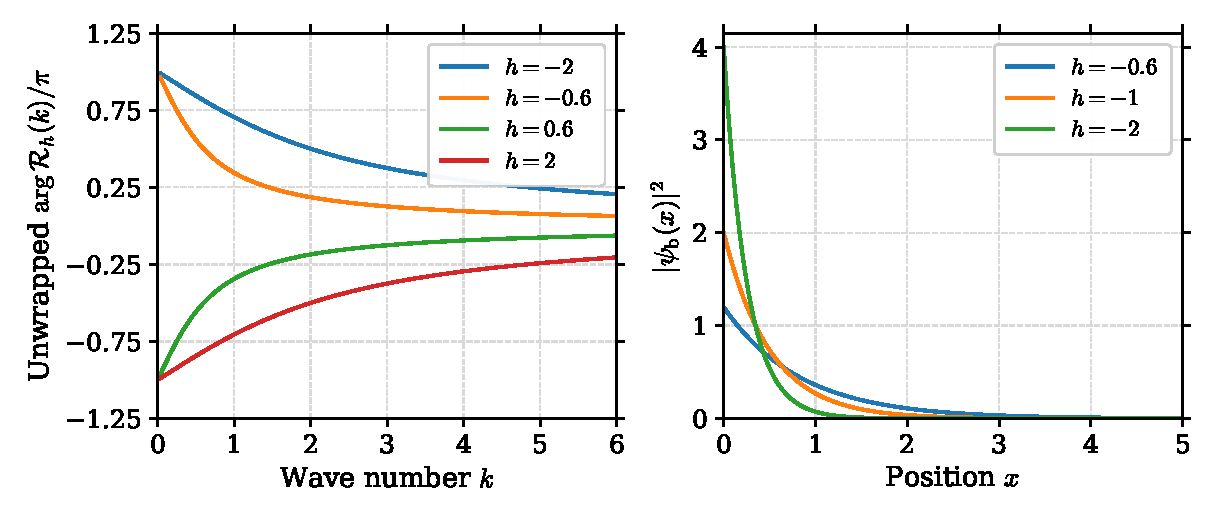
\includegraphics[width=.84\linewidth]{content/MathSkills/figures/geometry-highspin/robin_scattering.pdf}
\caption{不同自伴边界参数 $h$ 下的精确反射相位及归一化束缚态。左图用 $\arg\mathcal R_h(k)$ 的连续分支表征谱参数对散射的影响；右图仅对 $h<0$ 显示 $|\psi_{\mathrm b}(x)|^2$。两者共享同一个边界参数，没有对连续谱进行人为截断。}
\label{fig:ghs-r7-robin-scattering}
\end{figure}

一般度规上的边界不一定是一点，边界 Cauchy 数据可能属于无限维 Sobolev 空间；这时 $h$ 被边界上的自伴算子或 Lagrange 子空间取代，预解差通常也不再是秩一。半直线模型的重要性，在于自伴性、谱测度、负能束缚态及散射矩阵能够在同一套约定下逐式验证，从而为一般的边界谱问题提供最小的完整范例。

二维双曲空间的测地极坐标度规是 $\dd r^2+\sinh^2r\,\dd\theta^2$，故
\[
\Delta_{\mathbb H^2}=\partial_r^2+\coth r\,\partial_r
+\frac{1}{\sinh^2r}\partial_\theta^2.
\]
设 $\phi=R_m(r)\ee^{\ii m\theta}$，则方程 $-\Delta\phi=\lambda\phi$ 变为
\begin{equation}\label{eq:ghs-r6-hyperbolic-radial}
-R_m''-\coth r\,R_m'
+\frac{m^2}{\sinh^2r}R_m=\lambda R_m.
\end{equation}
在 $r\to\infty$ 时，$\coth r=1+O(\ee^{-2r})$ 且角势指数衰减，所以领先径向方程是
$-R''-R'=\lambda R$。令 $R\sim\ee^{sr}$ 后得 $s^2+s+\lambda=0$，根为
\[
s=-\frac12\pm\sqrt{\frac14-\lambda}.
\]
因此当 $\lambda=1/4+\rho^2$、$\rho\in\RR$ 时，远区两支行为是 $\ee^{-r/2\pm\ii\rho r}$。这里 $1/4$ 是连续谱的自然阈值；完整断言 $\operatorname{spec}(-\Delta_{\mathbb H^2})=[1/4,\infty)$ 且无 $L^2$ 点谱，仍需双曲空间调和分析或相应正性估计，不能只凭此渐近 ODE 作全谱证明。

球面角动量只描述角向分解，不能决定散射相位。若背景或势保持旋转对称，每个 $\ell$ 通道的径向自伴算子仍可能含不同的边界参数、束缚态与连续谱相移；相关可观测量要从其解析预解、Jost 解及壳上散射矩阵提取。在一般非球对称背景，各 $\ell$ 通道还会耦合成矩阵值散射问题。此时更普适的对象是完整的谱投影和散射算子，而不是把某一条球面高自旋定则推广成普遍结论。

一维边界问题说明了定义域为什么重要。对真正的标量、矢量或张量场，还需要确定其协变微分算子，之后才能从整个谱构造热核与 Green 函数。

\subsection{区间逆核的直接计算}
\label{app:ghs-spectral-tests}



对区间 $(0,L)$ 上的算子 $A=-\frac{\dd^2}{\dd x^2}+m^2$，$m>0$，取 Dirichlet 边界条件。对于固定源点 $y$，齐次方程的两侧解分别可取 $\sinh(mx)$ 与 $\sinh(m(L-x))$。要求 $G(x,y)$ 连续，且
$-\partial_xG(y^+,y)+\partial_xG(y^-,y)=1$，由此唯一得到
\begin{equation}\label{eq:ghs-dirichlet-green-interval}
 G_D(x,y)=\frac{\sinh(m x_<)\sinh[m(L-x_>)]}{m\sinh(mL)},
 \qquad x_<=\min(x,y),\quad x_>=\max(x,y).
\end{equation}
将 $G_D$ 对 $x$ 积分两次，可检查其是 $A^{-1}$ 的积分核。若将边界换成 Neumann，核的边界导数条件改变，零质量极限还要移除常数零模。这一完整计算说明 Green 函数的选择确实依赖算子定义域。



\section{一般理论之后的可解模型}

本节的模型只用于检验前面建立的母结构。每个模型都先明确自伴定义域，再从一般预解式或谱演算公式中取特例，而不反过来由特殊解推断一般理论。
\begin{exbox}[常系数分离边界的特征方程]\label{ex:math-sl-regular-robin-eigen}
取 $I=(0,\ell)$，令 $p=p_0>0$、$q=q_0\in\RR$、$w=w_0>0$。在 $L^2((0,\ell),w_0\dd x)$ 上令
\[
 AX=\frac{-p_0X''+q_0X}{w_0},
\]
并取定义域
\[
 \Dom(A)=\left\{X\in H^2(0,\ell):
 \begin{array}{l}
 a_1X(0)+a_2X^{[1]}(0)=0,\\
 b_1X(\ell)+b_2X^{[1]}(\ell)=0
 \end{array}\right\},
\]
其中边界系数取实数，且每端的两个系数不同时为零；这正是一个分离自伴实现。谱方程为
\[
 -p_0X''+q_0X=\lambda w_0X.
\]
令
\[
 k^2=\frac{\lambda w_0-q_0}{p_0},
 \qquad
 C_k(x):=\cos(kx),
 \qquad
 S_k(x):=
 \begin{cases}
 \dfrac{\sin(kx)}{k},&k\neq0,\\[1ex]
 x,&k=0.
 \end{cases}
\]
$C_k,S_k$ 都只依赖 $k^2$，并在 $k=0$ 处连续，因此不会漏掉阈值情形的线性解。通解写成
\[
 X(x)=A C_k(x)+B S_k(x),
 \qquad
 X^{[1]}(x)=p_0\bigl[-A k\sin(kx)+B\cos(kx)\bigr].
\]
代入两个端点条件得到关于 $(A,B)$ 的齐次线性系统，非零解存在的充要条件是
\begin{equation*}\det\begin{pmatrix}
 a_1&a_2p_0\\
 b_1\cos(k\ell)-b_2p_0k\sin(k\ell)&
 b_1S_k(\ell)+b_2p_0\cos(k\ell)
 \end{pmatrix}=0.
\end{equation*}
这个行列式只是一般判据 $\omega(\lambda)=0$ 在常系数模型中的显式形式。
\end{exbox}

\begin{exbox}[同一问题的 Green 核]\label{ex:math-sl-green-robin-constant}
对 $z\in\rho(A)$，分别求满足左、右分离边界条件的 $\phi_0(x,z),\psi_\ell(x,z)$。它们都是 $\cos(kx),\sin(kx)$ 的线性组合，且
\[
 \omega(z)=\mathcal W[\phi_0,\psi_\ell]\neq0.
\]
因此 Green 核无需重新推导，直接由\eqnrefs{eq:math-sl-green-regular-formula} 给出。若 $z$ 逼近某个简单本征值，$\omega(z)$ 的简单零点产生\eqnrefs{eq:math-sl-residue-formula} 的秩一极点；这把特征方程和受迫响应放在同一个解析函数中。
\end{exbox}
\begin{exbox}[半直线常势算子的预解式核]\label{ex:math-sl-halfline-resolvent}
在 $L^2(0,\infty)$ 上取
\[
 A=-\frac{\dd^2}{\dd x^2}+\nu^2,
 \qquad \nu>0,
\]
其 Robin 自伴定义域为
\[
 \Dom(A_h)=\{y\in H^2(0,\infty):y'(0)=hy(0)\},
 \qquad h\in\RR.
\]
无穷远是 极限点型，因此不再施加第二个边界条件。对 $z\in\rho(A_h)$，取
\[
 \kappa(z)=\sqrt{\nu^2-z},\qquad \Re\kappa(z)>0.
\]
无穷远 Weyl 解为 $\psi_\infty=\ee^{-\kappa x}$，左端适配解可取
\[
 \phi_0(x,z)=\cosh(\kappa x)+\frac{h}{\kappa}\sinh(\kappa x).
\]
由 $\omega=\phi_0'\psi_\infty-\phi_0\psi_\infty'=h+\kappa$，得到
\begin{equation}\label{eq:math-sl-halfline-explicit-green}
 G_z(x,\xi)=\frac{1}{\kappa(z)+h}
 \begin{cases}
 \phi_0(x,z)\ee^{-\kappa(z)\xi},&x\le\xi,\\
 \phi_0(\xi,z)\ee^{-\kappa(z)x},&\xi<x.
 \end{cases}
\end{equation}
自伴算子 $A_h$ 的本质谱（并且是绝对连续谱）为 $[\nu^2,\infty)$。若 $h<0$，方程 $\kappa+h=0$ 还产生一个离散本征值 $\lambda_b=\nu^2-h^2$；因此\eqnrefs{eq:math-sl-halfline-explicit-green} 的适用条件不仅是避开连续谱，还必须避开这个可能存在的离散极点。
\end{exbox}

\begin{exbox}[Laplace--Green 方法作用于半直线演化]\label{ex:math-sl-laplace-green-halfline}
对同一个 $A$ 求解 $u_t+Au=F$。Laplace 变换给出
\[
 \widehat u(s)=(s+A)^{-1}(u_0+\widehat F).
\]
在\eqnrefs{eq:math-sl-halfline-explicit-green} 中令 $z=-s$，即 $\kappa=\sqrt{\nu^2+s}$，便得到
\[
 \widehat u(x,s)=\int_0^\infty G_{-s}(x,\xi)
 \bigl(u_0(\xi)+\widehat F(\xi,s)\bigr)\dd\xi.
\]
因此时间变换后的空间问题没有产生新 Green 理论，它只是对同一个预解式在参数 $z=-s$ 处取值。
\end{exbox}
从这里开始统一采用酉 Fourier 变换
\begin{equation}\label{eq:math-sl-unitary-fourier-convention}
 \widehat f(k)=\frac{1}{\sqrt{2\pi}}
 \int_{\RR}\ee^{-\ii xk}f(x)\dd x,
 \qquad
 f(x)=\frac{1}{\sqrt{2\pi}}
 \int_{\RR}\ee^{\ii xk}\widehat f(k)\dd k.
\end{equation}
它把 $L^2(\RR,\dd x)$ 酉地映到 $L^2(\RR,\dd k)$；因此后面所有 Fourier 乘子、谱密度与传播公式都使用同一归一化，不再另外吸收 $2\pi$ 因子。

\begin{exbox}[全空间自由算子的 Green 核]\label{ex:math-sl-line-free-green}
取
\[
 A=-\frac{\dd^2}{\dd x^2}+\nu^2
 \quad\text{on }L^2(\RR),
 \qquad
 \Dom(A)=H^2(\RR).
\]
两端均为 极限点型，所以紧支撑预最小算子的闭包恰好就是上述自伴算子。对 $z\in\CC\setminus[\nu^2,\infty)$，令 $\kappa=\sqrt{\nu^2-z}$ 且 $\Re\kappa>0$。左右 Weyl 解分别为 $\ee^{\kappa x}$ 与 $\ee^{-\kappa x}$，从\eqnrefs{eq:math-sl-green-line} 得
\begin{equation*}G_z(x,\xi)=\frac{1}{2\kappa(z)}\ee^{-\kappa(z)|x-\xi|}.
\end{equation*}
不存在 $L^2$ 本征函数，谱 $[\nu^2,\infty)$ 完全为绝对连续谱；若改用能量变量 $\lambda=k^2+\nu^2$ 描述，则除阈值外的谱重数为 $2$，对应 $k=\pm\sqrt{\lambda-\nu^2}$ 两个传播通道。Fourier 变换只是该谱测度的一种显式对角化，实现
\[
 \widehat{Af}(k)=(k^2+\nu^2)\widehat f(k).
\]
若 $f\in L^2(\RR)$，其标量谱测度因此直接由
\[
 \mu_f(B)=\int_{\{k:\,k^2+\nu^2\in B\}}|\widehat f(k)|^2\dd k
\]
给出。选取 $\widehat f$ 的任意可测代表，并对 $\lambda>\nu^2$ 作变量代换 $k=\pm\sqrt{\lambda-\nu^2}$，便得到下面的绝对连续密度；等式按 Lebesgue 几乎处处理解：
\begin{equation*}\frac{\dd\mu_f}{\dd\lambda}(\lambda)
 =\frac{
 |\widehat f(\sqrt{\lambda-\nu^2})|^2+
 |\widehat f(-\sqrt{\lambda-\nu^2})|^2}
 {2\sqrt{\lambda-\nu^2}}.
\end{equation*}
两个 $k$ 分支正是谱重数 $2$ 的来源，而阈值处的 $1/\sqrt{\lambda-\nu^2}$ Jacobian 是能量变量谱密度的几何因子，并不表示存在离散本征态。
\end{exbox}

更一般地，若全线上的平移不变自伴算子在 Fourier 表象中由实可测符号 $\mathfrak a(k)$ 乘法表示，则相应无界自伴算子的定义域本身就是
\[
 \Dom(A)=\left\{f\in L^2(\RR):\mathfrak a(k)\widehat f(k)\in L^2(\RR,\dd k)\right\},
 \qquad
 \widehat{Af}=\mathfrak a\,\widehat f.
\]
谱定理在这里退化为逐 $k$ 的乘法演算。对一阶耗散问题还必须要求 $\mathfrak a$ 本质下有界，否则 $\ee^{-t\mathfrak a(k)}$ 在固定 $t>0$ 也可能无界，不能在 $L^2$ 上定义有界半群。在这一半有界假设下，一阶传播为
\begin{equation*}\widehat u(t,k)=\ee^{-t\mathfrak a(k)}\widehat u_0(k)
 +\int_0^t\ee^{-(t-s)\mathfrak a(k)}\widehat F(s,k)\dd s,
\end{equation*}
若二阶问题采用前述常阻尼传播，还要求相应的标量因子 $\Phi_{\mathfrak a(k)}(t),\Psi_{\mathfrak a(k)}(t)$ 在 $\mathfrak a(k)$ 的本质值域上有界；例如 $\mathfrak a(k)\ge0$ 时这一条件自动满足。此时二阶常阻尼传播为
\begin{equation*}\widehat u(t,k)=\Phi_{\mathfrak a(k)}(t)\widehat u_0(k)
 +\Psi_{\mathfrak a(k)}(t)\widehat u_1(k)
 +\int_0^t\Psi_{\mathfrak a(k)}(t-s)\widehat F(s,k)\dd s.
\end{equation*}
这不是一套平行于谱定理的“Fourier 方法”，而是把抽象谱表示具体实现为乘法算子的特例。

\begin{exbox}[纯点谱与 Fourier 谱的同一传播子]
\label{ex:math-sl-first-abstract-general}
\label{ex:math-sl-second-abstract-general}
\label{ex:math-sl-fourier-first-general}
\label{ex:math-sl-fourier-second-general}
同一个 Borel 函数演算在纯点谱与绝对连续谱中只改变“谱坐标”的写法。若 $A$ 具有紧预解式，\eqnrefs{eq:math-sl-duhamel-semigroup} 与\eqnrefs{eq:math-sl-abstract-second-order-formal} 分别成为
\begin{equation*}u(t)=\sum_n\left[
 \ee^{-\lambda_nt}u_{0,n}
 +\int_0^t\ee^{-\lambda_n(t-s)}F_n(s)\dd s
 \right]X_n,
\end{equation*}
以及
\begin{equation*}u(t)=\sum_n\left[
 \Phi_{\lambda_n}(t)u_{0,n}
 +\Psi_{\lambda_n}(t)u_{1,n}
 +\int_0^t\Psi_{\lambda_n}(t-s)F_n(s)\dd s
 \right]X_n.
\end{equation*}

若全线平移不变算子由 Fourier 乘子 $\mathfrak a(k)$ 对角化，则沿用\eqnrefs{eq:math-sl-unitary-fourier-convention} 的酉归一化。一阶传播写成
\begin{equation*}\widehat u(t,k)=\ee^{-t\mathfrak a(k)}\widehat u_0(k)
 +\int_0^t\ee^{-(t-s)\mathfrak a(k)}\widehat F(s,k)\dd s,
\end{equation*}
并在物理空间成为
\begin{equation*}u(x,t)=\frac{1}{\sqrt{2\pi}}\int_{\RR}\ee^{\ii xk}
 \left[\ee^{-t\mathfrak a(k)}\widehat u_0(k)
 +\int_0^t\ee^{-(t-s)\mathfrak a(k)}\widehat F(s,k)\dd s\right]\dd k.
\end{equation*}
二阶传播则为
\begin{equation*}\widehat u(t,k)=\Phi_{\mathfrak a(k)}(t)\widehat u_0(k)
 +\Psi_{\mathfrak a(k)}(t)\widehat u_1(k)
 +\int_0^t\Psi_{\mathfrak a(k)}(t-s)\widehat F(s,k)\dd s.
\end{equation*}
对一阶问题取 $\mathfrak a(k)=k^2$ 得到自由扩散；对二阶问题再取 $b=0$、$\mathfrak a(k)=k^2$ 得到自由波动。离散求和与 Fourier 积分的区别因此只来自谱测度是原子测度还是 Lebesgue 型测度。
\end{exbox}

\begin{exbox}[含时非齐次边界条件的齐次化]\label{ex:math-sl-time-lifting-template}
若一阶方程 $u_t+\tau u=F$ 带有 $B_au=g_a(t)$、$B_bu=g_b(t)$，先选 $h_b(x,t)$ 匹配这两个边界值，并令 $u=v+h_b$。则 $v$ 满足固定齐次自伴边界条件，而
\[
 v_t+Av=F-\partial_t h_b-\tau h_b.
\]
因此右端投影到谱测度后即可直接使用\eqnrefs{eq:math-sl-duhamel-semigroup}。二阶阻尼问题则把修正项替换为
\[
 -\partial_t^2h_b-b\partial_t h_b-\tau h_b.
\]
这个例子也说明为什么 提升 必须发生在谱展开之前：只有齐次化以后，时间演化才由一个固定自伴算子 $A$ 控制。
\end{exbox}

本章最终得到一条闭合的算子链。系数与权函数先确定微分表达式；最小/最大算子和 Lagrange 边界型再确定允许的自伴扩张；Weyl 分类判断奇异端点还留下多少边界自由度。自伴算子确定以后，谱测度统一产生 Borel 函数演算、预解式 与含时传播，Green 核只是预解式的坐标积分核。有限正则区间的特征函数级数与全线 Fourier 积分因此不是两套理论，而是同一谱积分在不同谱型下的具体实现。
谱的定义不只是分类本征值。真正控制算符在参数 $z$ 附近如何变化的是预解算符
\[
R(z;A)=(A-zI)^{-1},
\qquad z\in\rho(A).
\]
若 $z,w\in\rho(A)$，则
\[
(A-zI)^{-1}-(A-wI)^{-1}
=(z-w)(A-zI)^{-1}(A-wI)^{-1}.
\]
验证只需把右端通分：
\[
\begin{aligned}
&(A-zI)^{-1}\bigl[(A-wI)-(A-zI)\bigr](A-wI)^{-1}\\
&\qquad=(z-w)(A-zI)^{-1}(A-wI)^{-1}.
\end{aligned}
\]
因此有第一预解恒等式
\begin{equation*}\boxed{
R(z;A)-R(w;A)=(z-w)R(z;A)R(w;A)
}.\end{equation*}

它立即给出预解集的开性。固定 $z_0\in\rho(A)$，写
\[
A-zI=(A-z_0I)\bigl[I-(z-z_0)R(z_0;A)\bigr].
\]
若
\[
|z-z_0|\,\|R(z_0;A)\|<1,
\]
第二个因子可用 Neumann 级数求逆：
\[
\bigl[I-(z-z_0)R(z_0;A)\bigr]^{-1}
=\sum_{n=0}^\infty (z-z_0)^nR(z_0;A)^n.
\]
所以 $z$ 仍属于预解集。于是 $\rho(A)$ 是开集，
\[
\boxed{\sigma(A)\text{ 是闭集}.}
\]
同时在每个预解集连通分支内，$R(z;A)$ 是算符值解析函数。这是后面 Fredholm 预解核与解析 Fredholm 理论的算符基础。

对自伴算符还有更强的估计。若 $z=a+ib$、$b\neq0$，前面已经证明
\[
\|(A-zI)\psi\|\ge |b|\,\|\psi\|.
\]
因此
\begin{equation*}\boxed{
\|R(z;A)\|\le \frac1{|\operatorname{Im}z|}
}.\end{equation*}
这说明当复参数离实轴有固定距离时，自伴算符的逆不会失控；真正可能发生奇异行为的地方只能靠近实谱。
抽象定义必须通过一个真正没有普通本征矢的例子来理解。取
\[
\mathcal H=L^2([0,1]),
\]
并定义有界自伴乘法算符
\[
(M_xf)(x)=x f(x).
\]
因为
\[
\langle f|M_xg\rangle
=\int_0^1 f^*(x)xg(x)\,\dd x
=\langle M_xf|g\rangle,
\]
所以 $M_x=M_x^\dagger$，且 $\|M_x\|=1$。

先看普通本征值方程
\[
x f(x)=\lambda f(x).
\]
这等价于
\[
(x-\lambda)f(x)=0
\]
几乎处处成立。若 $\lambda\in[0,1]$，那么 $f$ 只能支撑在单点 $x=\lambda$ 上；单点的 Lebesgue 测度为零，所以任何 $L^2$ 函数都只能是零元。因此
\[
\sigma_{\mathrm p}(M_x)=\varnothing.
\]

但这不意味着谱为空。对 $z\notin[0,1]$，有
\[
(M_x-zI)^{-1}g(x)=\frac{g(x)}{x-z},
\]
并且
\[
\left\|\frac1{x-z}\right\|_{L^\infty([0,1])}
=\frac1{\operatorname{dist}(z,[0,1])}<\infty.
\]
所以
\[
z\notin[0,1]\quad\Longrightarrow\quad z\in\rho(M_x).
\]
反过来，若 $\lambda\in[0,1]$，先逐项核对连续谱定义。方程
\[
(M_x-\lambda I)f=0
\]
仍只有零解，所以 $M_x-\lambda I$ 是单射。其值域不是整个 $L^2([0,1])$：例如常数函数 $g=1$ 若属于值域，就必须有
\[
f(x)=\frac{1}{x-\lambda},
\]
但该函数在 $\lambda$ 附近不平方可积。

另一方面值域是稠密的。若 $h$ 与值域正交，则对所有 $f\in L^2([0,1])$ 有
\[
0=\langle h|(M_x-\lambda I)f\rangle
=\langle (M_x-\lambda I)h|f\rangle,
\]
从而 $(x-\lambda)h(x)=0$ 几乎处处。由于单点集合测度为零，只能有 $h=0$。故值域正交补为零，值域稠密。

最后取归一化函数列 $f_n$ 集中在 $\lambda$ 附近，例如支撑在长度趋于零的小区间内，则
\[
\|(M_x-\lambda I)f_n\|\to0,
\qquad \|f_n\|=1.
\]
因此值域上的逆必无界。于是对每个 $\lambda\in[0,1]$，$M_x-\lambda I$ 都满足“单射、值域稠密但非满射、逆无界”，正是连续谱情形。故
\[
\boxed{\sigma(M_x)=[0,1]}
\]
而整个谱都是连续谱。

这个例子把形式符号
\[
M_x|\lambda\rangle=\lambda|\lambda\rangle
\]
的真正含义暴露出来：$|\lambda\rangle$ 不属于 $L^2([0,1])$，而应理解成类似 $\delta(x-\lambda)$ 的广义本征态。下一章的分布理论正是为这种对象提供严格语言。
在整条实线上取
\[
P=-\ii\frac{\dd}{\dd x}
\]
并以合适的 Sobolev 空间 $H^1(\mathbb R)$ 为定义域。Fourier 变换满足
\[
\mathcal F(P\psi)(k)=k\widehat\psi(k).
\]
因此
\[
P=\mathcal F^{-1}M_k\mathcal F,
\]
也就是说动量算符与 Fourier 空间中的实变量乘法算符酉等价。由酉等价保持谱，得到
\[
\boxed{\sigma(P)=\mathbb R}
\]
且没有 $L^2(\mathbb R)$ 中的普通平面波本征矢。

形式本征方程
\[
-\ii\psi_p'(x)=p\psi_p(x)
\]
给出
\[
\psi_p(x)=C \ee^{\ii px}.
\]
它不平方可积，但可以用分布归一化
\[
\langle p|p'\rangle=\delta(p-p')
\]
以及完备关系
\[
\int_{-\infty}^{\infty}|p\rangle\langle p|\,\dd p=I
\]
来使用。这些公式不是有限维正交基公式的字面延伸，而是谱测度与分布语言下的连续版本。
量子力学把自伴算符与可观测量联系起来，但更深的一层结构是：自伴算符生成一参数幺正群。若 $A=A^\dagger$，谱定理允许定义
\[
U(t)=\ee^{-\ii tA}
=\int_{\sigma(A)}\ee^{-\ii t\lambda}\,\dd E_A(\lambda).
\]
因为 $|\ee^{-\ii t\lambda}|=1$，有
\[
U(t)^\dagger U(t)=I,
\qquad
U(t+s)=U(t)U(s),
\qquad
U(0)=I.
\]
所以 $U(t)$ 是一参数幺正群。

若 $\psi\in D(A)$，则可以在强意义下求导：
\[
\begin{aligned}
\frac{U(t+h)\psi-U(t)\psi}{h}
&=U(t)\frac{\ee^{-\ii hA}-I}{h}\psi\\
&\longrightarrow -iU(t)A\psi.
\end{aligned}
\]
因此
\begin{equation*}\boxed{
i\frac{\dd}{\dd t}U(t)\psi=A U(t)\psi
}.\end{equation*}
这就是抽象 Schrodinger 方程的 Hilbert 空间版本：动力学不是额外写上去的，而是由自伴生成元的谱函数演算产生。

Stone 定理的反方向同样重要：若 $U(t)$ 是强连续的一参数幺正群，那么存在唯一自伴算符 $A$ 使
\[
U(t)=\ee^{-\ii tA}.
\]
因此“自伴性”不只是保证本征值为实数；它同时是连续幺正时间演化的生成元条件。对无界 Hamiltonian，若只验证形式对称而没有验证真正自伴，就还没有充分保证全局幺正演化。
一阶动量算符已经说明定义域的重要性。二阶算符的例子更直观。取
\[
A=-\frac{\dd^2}{\dd x^2},
\qquad 0<x<L.
\]
对 $\psi,\phi\in H^2(0,L)$，两次分部积分给出 Green 边界型
\[
\begin{aligned}
\langle\psi|A\phi\rangle-\langle A\psi|\phi\rangle
&=\left[\psi^*{}'\phi-\psi^*\phi'\right]_{0}^{L}.
\end{aligned}
\]
要使算符自伴，必须选择定义域，使这个边界型对定义域内任意 $\psi,\phi$ 都消失，并且伴算符不再拥有更大的定义域。

Dirichlet 条件
\[
\psi(0)=\psi(L)=0
\]
给出本征方程
\[
-\psi''=\lambda\psi
\]
的解
\[
\psi_n(x)=\sqrt{\frac2L}\sin\frac{n\pi x}{L},
\qquad
\lambda_n=\left(\frac{n\pi}{L}\right)^2,
\qquad n=1,2,\ldots.
\]
而 Neumann 条件
\[
\psi'(0)=\psi'(L)=0
\]
给出
\[
\psi_n(x)=
\begin{cases}
L^{-1/2},&n=0,\\[3pt]
\sqrt{\dfrac2L}\cos\dfrac{n\pi x}{L},&n\ge1,
\end{cases}
\]
\[
\lambda_n=\left(\frac{n\pi}{L}\right)^2,
\qquad n=0,1,2,\ldots.
\]
同一个形式微分表达式 $-\dd^2/\dd x^2$，因为定义域和边界条件不同，谱中是否包含零模已经发生变化。

更一般的 Robin 条件可以写成
\[
\psi'(0)=h_0\psi(0),
\qquad
\psi'(L)=-h_L\psi(L),
\]
其中 $h_0,h_L\in\mathbb R$。把两组满足相同 Robin 条件的函数代入边界型，端点项逐一相消，所以得到对称实现；在规则 Sturm--Liouville 情形中这类分离实边界条件给出自伴实现。这里最重要的不是记住几类条件，而是掌握检查方法：
\[
\boxed{
\text{微分表达式}
\;\longrightarrow\;
\text{分部积分边界型}
\;\longrightarrow\;
\text{允许的自伴定义域}
}.
\]
\chapref{chap:integral-equations}要讨论非自伴积分核。这里先把所需的 Hilbert 空间结构建立起来。对有界算符 $K$，正算符
\[
K^\dagger K\ge0
\]
可以通过谱函数演算定义
\[
|K|=(K^\dagger K)^{1/2}.
\]
存在部分等距算符 $U$ 使
\begin{equation*}\boxed{K=U|K|},\end{equation*}
这称为极分解。有限维矩阵的 ``相位 $\times$ 正矩阵'' 分解就是它的特例。

若 $K$ 还是紧算符，则 $|K|$ 是紧自伴正算符。由紧自伴谱定理，可以找到正交归一向量 $\psi_n$ 与非负本征值 $s_n\to0$，满足
\[
|K|\psi_n=s_n\psi_n.
\]
对 $s_n>0$，定义
\[
\phi_n=\frac{K\psi_n}{s_n}.
\]
则
\[
\langle\phi_m|\phi_n\rangle
=\frac{\langle\psi_m|K^\dagger K\psi_n\rangle}{s_ms_n}
=\delta_{mn}.
\]
于是
\begin{equation*}\boxed{
Kf=\sum_{n}s_n\langle\psi_n|f\rangle\phi_n
}\end{equation*}
在适当子空间上成立。这就是无限维的奇异值分解。\chapref{chap:integral-equations}第一类积分方程的不适定性，本质上就是 $s_n\to0$ 使逆问题中的系数 $1/s_n$ 发散。
有限维双系统中的任意纯态
\[
|\Psi\rangle\in\mathcal H_A\otimes\mathcal H_B
\]
都可以写成
\begin{equation}
\boxed{
|\Psi\rangle
=\sum_{r=1}^{R}s_r|a_r\rangle\otimes|b_r\rangle,
\qquad s_r>0,
}
\label{eq:schmidt-decomposition}
\end{equation}
其中 $\{|a_r\rangle\}$、$\{|b_r\rangle\}$ 分别正交归一。这不是额外的量子公设，而是矩阵奇异值分解的直接结果。

选定基 $\{|i\rangle_A\}$、$\{|j\rangle_B\}$，写
\[
|\Psi\rangle=\sum_{ij}C_{ij}|i\rangle_A\otimes|j\rangle_B.
\]
对系数矩阵作 SVD：
\[
C=U\Sigma V^\dagger.
\]
若
\[
\Sigma=\operatorname{diag}(s_1,\ldots,s_R,0,\ldots),
\]
并定义
\[
|a_r\rangle=\sum_iU_{ir}|i\rangle_A,
\qquad
|b_r\rangle=\sum_jV_{jr}^*|j\rangle_B,
\]
立即得到 \eqnrefs{eq:schmidt-decomposition}。

若只有一个非零 Schmidt 系数，态就是简单张量；若至少两个 $s_r\neq0$，就不可能写成
\[
|a\rangle\otimes|b\rangle,
\]
即为纠缠态。若 $\|\Psi\|=1$，则
\[
\sum_rs_r^2=1.
\]
因此“简单张量之和一般不能再化成简单张量”可以被精确量化为 Schmidt 秩 $R$ 大于 1。




抽象扩张和谱测度已经给出统一规则。以下在区间与半直线模型中逐项检查伴随域、边界型、谱投影和能量形式，说明每个域条件怎样改变解与谱。

\section{分部积分能证明什么}

区间动量算子的闭包 \(P=(-\ii\partial_x,H_0^1(0,1))\) 对称。对 \(f,g\in H^1(0,1)\)，逐次使用一维分部积分得
\[
\langle -\ii g',f\rangle-\langle g,-\ii f'\rangle
=-\ii[\overline f g]_0^1.
\]
若两函数端点均为零，边界项消失，所以 \(P\subset P^*\)。然而已算出 \(D(P^*)=H^1(0,1)\)，严格大于 \(H_0^1(0,1)\)：常数函数就在伴随域，却不在 \(D(P)\)。这给出一个对称而不自伴的完整反例。

\begin{definition}[对称与自伴]
稠密定义算子 \(A\) 对称，意为 \(\langle Ag,f\rangle=\langle g,Af\rangle\) 对所有 \(f,g\in D(A)\) 成立，即 \(A\subset A^*\)。若还满足 \(D(A)=D(A^*)\)，从而 \(A=A^*\)，称 \(A\) 自伴。
\end{definition}

端点条件可以补足动量算子的定义域。固定 \(\theta\in[0,2\pi)\)，令
\[
D(P_\theta)=\{f\in H^1(0,1):f(1)=\ee^{\ii\theta}f(0)\},
\qquad P_\theta f=-\ii f'.
\]
该域上边界项为零。要检查伴随域，不能止于这句话：若 \(g\in D(P_\theta^*)\)，先以紧支函数测试得 \(g\in H^1\)；再让 \(f(0)\) 任取复数，且 \(f(1)=\ee^{\ii\theta}f(0)\)，边界项消失要求 \(\overline{g(1)}\ee^{\ii\theta}=\overline{g(0)}\)，即 \(g(1)=\ee^{\ii\theta}g(0)\)。故 \(D(P_\theta^*)=D(P_\theta)\)，它确实自伴。解 \(-\ii f'=\lambda f\) 得 \(f(x)=C\ee^{\ii\lambda x}\)，边界条件给 \(\lambda=2\pi n+\theta\)，\(n\in\ZZ\)。


\par
\begin{workedexample}
在 \(D(S_R)=\{f\in H^2(0,1):f'(0)=\alpha f(0),\ f'(1)=-\beta f(1)\}\) 中取实数 \(\alpha,\beta\)。用边界型检验对称性，再通过任意选择 \(f(0),f(1)\) 求 \(D(S_R^*)\)，证明它自伴。


\textbf{解。} 对 \(S_R=-\partial_x^2\)，分部积分给出边界型
\[
\langle S_Rg,f\rangle-\langle g,S_Rf\rangle=[\overline{f'}g-\overline f g']_0^1.
\]
在 \(g'(0)=\alpha g(0),\ g'(1)=-\beta g(1)\) 上，因 \(\alpha,\beta\in\RR\)，两端项分别为实数系数乘 \(\overline{f(j)}g(j)\)，相减后为零，故对称。伴随域中的函数满足同一边界型对所有满足原边界条件的 \(f\) 消失；端点值可独立任取，遂强制 \(g'(0)=\alpha g(0)\)、\(g'(1)=-\beta g(1)\)。因此 \(D(S_R^*)=D(S_R)\)，算子自伴。
\end{workedexample}
\par
\section{二阶算子的边界型}

对 \(S_0=-\partial_x^2\) 取初始域 \(C_c^\infty(0,1)\)。若 \(g\in D(S_0^*)\)，则某个 \(h\in L^2\) 满足 \(\int\overline g(-\varphi'')=\int\overline h\varphi\) 对所有紧支光滑 \(\varphi\) 成立。这正说 \(-g''=h\) 为弱导数。把 \(h\) 积分两次，并减去所得原函数，余下的分布二阶导数为零，因而是仿射函数；所以 \(g\in H^2(0,1)\)。反向分部积分立即成立，故 \(D(S_0^*)=H^2(0,1)\)，称最大域。\(S_0\) 的图闭包的域为 \(H_0^2(0,1)\)，即 \(H^2\) 中函数值和一阶导数在两端均为零的函数；这称最小域。注意最小域比 Dirichlet 域还小，因为后者不限制端点导数。于是域的包含关系清楚：\(H_0^2\subset H_0^1\subset H^1\)，而 Dirichlet 域 \(H^2\cap H_0^1\) 介于 \(H_0^2\) 与 \(H^2\) 之间。在最大域中，分部积分两次给出
\[
\langle S_0^*g,f\rangle-\langle g,S_0^*f\rangle
=\bigl[\overline{f'}g-\overline f g'\bigr]_0^1.
\]
这个边界型同时含函数值和导数值，所以二阶算子比动量多需要一组端点条件。若取 \(D(S_D)=\{f\in H^2:f(0)=f(1)=0\}\)，边界型在域内消失；若 \(g\in D(S_D^*)\)，令 \(f'(0),f'(1)\) 独立变化，又迫使 \(g(0)=g(1)=0\)。于是 \(S_D\) 自伴。固定导数为零的 Neumann 域与同样推理得到自伴；它容许常数零模，而 Dirichlet 域不容许。

独立改变端点条件不能只看边界型的一个方向。比如只要求 \(f(0)=f(1)=0\) 而忘记域必须落在 \(H^2\)，那么 \(-f''\) 可能根本不属于 \(L^2\)，算子尚未定义。完整检查总是先确定最大域，再要求边界型在候选域内为零，最后算候选域的伴随是否仍是它自己。

Robin 条件也可把边界响应连续地反映到能谱。两端取同一非负参数 \(h\)：\(f'(0)=hf(0)\)、\(f'(1)=-hf(1)\)。设正本征值为 \(k^2\)，通解 \(f=A\cos kx+B\sin kx\)。左条件给 \(B=hA/k\)；把它代入右条件并消去非零 \(A\)，得到
\[
(h^2-k^2)\sin k+2hk\cos k=0.
\]
当 \(h=0\) 时还要单独检查 \(k=0\)，它给 Neumann 零模；当 \(h>0\) 时零模消失。这个小计算展示边界参数进入谱的具体位置，也提醒我们除以 \(k\) 前必须先处理 \(k=0\)。

代入具体参数看能级怎样随边界参数移动。\(h=0\) 时方程退化为 \(-k^2\sin k=0\)，正本征值 \(k=n\pi\)；此时 \(k=0\) 要单独看：通解 \(f=A+Bx\)，两端 \(f'(0)=f'(1)=B=0\) 迫使 \(B=0\)，留下常数解 \(f=A\)，正是 Neumann 零模。\(h=1\) 时方程为 \((1-k^2)\sin k+2k\cos k=0\)：左端在 \(k=1\) 为正、在 \(k=\pi/2\) 为负，故最低正本征值落在 \((1,\pi/2)\) 内；它随 \(h\) 连续变化，\(h=0\) 时退回 \(k=0\) 零模。这就是“边界参数进入谱”的具体位置。




\section{亏量空间记录缺少的边界数据}

区间动量在零端点域上对称却不自伴；给端点增加相位关系以后成为自伴。能否一般地判断一个对称算子是否容许这样的补充？非实数 \(\pm\ii\) 不可能是对称算子的本征值，因为对称算子的本征值实。因此伴随在这两个值上的核只记录原定义域尚未控制的方向。

\begin{definition}[亏量空间]
对稠密定义、闭且对称的算子 \(S\)，定义 \(\mathcal N_+=\ker(S^*-\ii I)\)、\(\mathcal N_-=\ker(S^*+\ii I)\)，其维数 \(n_+,n_-\) 称亏格。
\end{definition}

在区间动量 \(P=(-\ii\partial_x,H_0^1(0,1))\) 上，\(P^*f=\ii f\) 给 \(f'=-f\)，所以 \(\mathcal N_+=\operatorname{span}\{\ee^{-x}\}\)；\(P^*f=-\ii f\) 给 \(f'=f\)，所以 \(\mathcal N_-=\operatorname{span}\{\ee^x\}\)。有限区间上二者均平方可积，亏格为 \((1,1)\)。端点相位 \(\theta\) 正是一维亏空间间酉映射的一个复相位。

\begin{theorem}[von Neumann 扩张定理]
设 \(S\) 为稠密定义、闭且对称的算子。它有自伴扩张当且仅当 \(n_+=n_-\)。每个自伴扩张由酉映射 \(U:\mathcal N_+\to\mathcal N_-\) 给出，其域为
\[
D(S_U)=D(S)\mathbin{\dot+}\{u+Uu:u\in\mathcal N_+\},
\qquad S_U(f+u+Uu)=Sf+\ii u-\ii Uu.
\]
\end{theorem}

\begin{proof}
这里 \(\dot+\) 表示每个向量具有唯一的分解。伴随算子 \(S^*\) 是闭的，所以在 \(D(S^*)\) 上，
\[
 (f,g)_G=\langle f,g\rangle+\langle S^*f,S^*g\rangle
\]
给出一个完备的内积。闭性也使 \(D(S)\) 成为这个图内积下的闭子空间。令 \(M\) 是它的正交补。若 \(h\in M\)，则对一切 \(f\in D(S)\) 有
\[
 \langle f,h\rangle+\langle Sf,S^*h\rangle=0.
\]
后一等式按伴随的定义说明 \(S^*h\in D(S^*)\)，而且 \(S^*(S^*h)=-h\)。它还说明 \(S^*h\in M\)：把 \(h\) 换成 \(S^*h\) 再与任意 \(f\in D(S)\) 取图内积，所得两项恰好相消。因此 \(S^*\) 在 \(M\) 上的平方是 \(-I\)。任取 \(h\in M\)，直接计算
\[
 h_+=\frac{h-\ii S^*h}{2},\qquad
 h_-=\frac{h+\ii S^*h}{2},\qquad
 S^*h_+=\ii h_+,\quad S^*h_-=-\ii h_-.
\]
我们得到伴随域的分解
\begin{equation}
 D(S^*)=D(S)\mathbin{\dot+}\mathcal N_+\mathbin{\dot+}\mathcal N_-.
 \label{eq:math-von-neumann-decomposition}
\end{equation}
三项在图内积下两两正交；例如 \(u\in\mathcal N_+\)、\(v\in\mathcal N_-\) 时，\((u,v)_G=\langle u,v\rangle+\langle\ii u,-\ii v\rangle=0\)。这一步解释了为何原算子域之外恰好只有两个“未配对”的方向，而不是任意多种边界数据。

现在把对称性写成伴随域上的边界型
\[
 B(f,g)=\langle S^*f,g\rangle-\langle f,S^*g\rangle.
\]
含有 \(D(S)\) 分量的项全为零。对 \(u_+,v_+\in\mathcal N_+\) 与 \(u_-,v_-\in\mathcal N_-\)，直接代入 \(S^*u_+=\ii u_+\)、\(S^*u_-=-\ii u_-\) 得
\[
 B(u_++u_-,v_++v_-)
 =2\ii\bigl(\langle u_+,v_+\rangle-\langle u_-,v_-\rangle\bigr).
\]
两种亏方向的交叉项自动为零。若把扩张域选成 \(D(S)\dot+\{u+Uu:u\in\mathcal N_+\}\)，上式为零的充要条件是 \(U\) 保内积。只有当 \(U\) 还映满 \(\mathcal N_-\) 时，扩张的伴随域才不会留下额外方向。确实，设 \(g=f+v_++v_-\in D(S_U^*)\)，逐一拿 \(u+Uu\) 测试边界型，得到 \(\langle u,v_+\rangle=\langle Uu,v_-\rangle\) 对一切 \(u\)。若 \(U\) 酉，则 \(v_-=Uv_+\)，故 \(g\in D(S_U)\)。

反向也能直接检验，而不必把“极大”当作未解释的口号。设 \(A\) 是 \(S\) 的任意自伴扩张；其域在分解~\cref{eq:math-von-neumann-decomposition} 中除 \(D(S)\) 外给出某个子空间 \(L\subset\mathcal N_+\oplus\mathcal N_-\)。对 \((u_+,u_-)\in L\) 取 \(B(u_++u_-,u_++u_-)=0\)，得到 \(\|u_+\|=\|u_-\|\)。所以投影 \(L\to\mathcal N_+\) 是单射，并把 \(L\) 写成一个保内积映射 \(U:M\to\mathcal N_-\) 的图，其中 \(M\subset\mathcal N_+\)。由于自伴算子闭，\(L\) 对图范数闭；在 \(L\) 上两个投影的范数相等，因而 \(M\) 也是闭子空间。若 \(M\ne\mathcal N_+\)，便可取非零 \(v_+\perp M\)。边界型公式给 \(B(v_+,u+Uu)=0\) 对所有 \(u\in M\)，所以 \(v_+\in D(A^*)\)；但 \(v_+\notin D(A)\)，与自伴性矛盾。故 \(M=\mathcal N_+\)。

若 \(U(M)\ne\mathcal N_-\)，同样取非零 \(v_-\perp U(M)\)，得到 \(v_-\in D(A^*)\setminus D(A)\)，仍矛盾。于是 \(U\) 必须映满，正是两亏空间间的酉映射；它存在当且仅当两空间维数相等。

\end{proof}

图内积的证明并没有假定微分表达式或端点值，所以定理可用于一般闭对称算子；具体端点条件仍须把 \(u+Uu\) 翻译回函数的边界数据。它并不说任意写一个端点条件就能自伴：条件必须让伴随域恰好等于所选域。

在半直线 \((0,\infty)\) 上重新取 \(P=-\ii\partial_x\) 与域 \(H_0^1(0,\infty)\)。伴随域仍为 \(H^1(0,\infty)\)，亏量方程仍给 \(\ee^{-x}\) 与 \(\ee^x\)，但后者不平方可积，于是亏格为 \((1,0)\)。定理表明半直线动量没有自伴扩张。端点只能让平移向一个方向离开半直线，无法形成对所有正负时间都可逆的酉平移群。

同在半直线，二阶表达式却给不同答案。令 \(S=-\partial_x^2\) 从 \(C_c^\infty(0,\infty)\) 闭合而来。伴随最大域中的亏量方程 \(-f''=\pm\ii f\) 各有两支指数解，但每个符号都恰有一支在无穷远平方可积，所以 \((n_+,n_-)=(1,1)\)。一个边界参数足以形成自伴扩张：\(D(S_\gamma)=\{f\in H^2(0,\infty):f'(0)=\gamma f(0)\}\)，其中 \(\gamma\in\RR\)。无穷远边界型对 \(H^2\) 函数消失；在零点，候选域内边界型消失，而让 \(f(0)\) 任取又使伴随域满足同一关系。若 \(\gamma<0\)，\(f(x)=\sqrt{-2\gamma}\,\ee^{\gamma x}\) 归一化且满足 \(S_\gamma f=-\gamma^2f\)。同一自由微分式会因边界吸引产生一个负能束缚态。


\par
\begin{workedexample}
对半直线上的 \(-\partial_x^2\) 与初始域 \(C_c^\infty(0,\infty)\)，解 \(-f''=\pm\ii f\) 并逐个判断平方可积性，得到其亏格。再说明为何零端点值和实 Robin 条件都可能给自伴扩张，而半直线动量不能。


\textbf{解.} 方程 \(-f''=\pm\ii f\) 的特征根在每个符号下各有一根实部为正、一根实部为负；半直线上恰有一个指数解平方可积，故亏格为 \((1,1)\)。实 Robin 条件 \(f'(0)=\gamma f(0)\)（含 Dirichlet 极限）使边界型消失并给出自伴扩张。动量 \(-\ii\partial_x\) 的两亏格不相等：一侧有一个可积指数解，另一侧没有，故半直线动量没有自伴扩张。
\end{workedexample}
\par
\section{同一能量表达式的三种自伴实现}

对 \(-\partial_x^2\) 的 Dirichlet 域，归一化本征函数为 \(\sqrt2\sin(n\pi x)\)，本征值 \(n^2\pi^2\)，\(n\ge1\)。Neumann 域的本征函数为 \(1\) 与 \(\sqrt2\cos(n\pi x)\)，本征值 \(0\) 与 \(n^2\pi^2\)。若两端接起来，采用 \(f(1)=f(0)\)、\(f'(1)=f'(0)\)，则本征函数为 \(\ee^{2\pi\ii nx}\)，本征值 \((2\pi n)^2\)，\(n\in\ZZ\)。这三种谱差别完全来自定义域。

另一个连续可调的选择是实参数 \(\alpha,\beta\) 的 Robin 条件 \(f'(0)=\alpha f(0)\)、\(f'(1)=-\beta f(1)\)。它仍令边界型消失，且伴随计算会重得同样两个条件。物理上，参数改变了边界处的响应；数学上，它改变了自伴实现，也就改变能级。闭区间二阶算子还有更一般的耦合端点条件，亏量空间的二维酉映射给出其系统分类。

\begin{example}[区间能谱与物理时间的恢复]
这里区间坐标 \(x\in(0,1)\) 已无量纲化，\(S_D=-\partial_x^2\) 的本征值也是无量纲数；取无量纲演化参数 \(s\)。Fourier 正弦系给 \(\psi=\sum_{n\ge1}c_n\sqrt2\sin(n\pi x)\) 且 \(\sum|c_n|^2=\|\psi\|^2\)。定义
\[
U(s)\psi=\sum_{n\ge1}\ee^{-\ii n^2\pi^2s}c_n\sqrt2\sin(n\pi x).
\]
每个系数只乘模为一的相位，因此 Parseval 恒等式 \cref{eq:math-parseval} 给 \(\|U(s)\psi\|=\|\psi\|\)，而 \(U(s+r)=U(s)U(r)\) 逐系数成立。对满足 \(\sum n^4|c_n|^2<\infty\) 的态，可逐项在 \(L^2\) 中求导并得到 \(\ii\partial_s\psi=S_D\psi\)。

若要恢复物理长度 \(L\)、粒子质量 \(m\) 和时间 \(t\)，令无量纲坐标
\(x=x_{\rm phys}/L\)。链式法则给出
\[
\partial_x=L\partial_{x_{\rm phys}},\qquad
-\partial_x^2=L^2(-\partial_{x_{\rm phys}}^2),\qquad
H=\frac{\hbar^2}{2mL^2}S_D.
\]
比较 \(\exp(-\ii Ht/\hbar)\) 与 \(U(s)\)，得到
\(s=\hbar t/(2mL^2)\)。这个无量纲时间同时保证了能量相位的量纲正确。
\end{example}

Stone 定理把这个逐模构造推广到任何自伴算子，包括没有离散本征函数基的情形。




\section{谱测度把“对角化”推广到连续能量}

\begin{example}[乘法算子的自伴域与连续谱]
在 $L^2(\RR)$ 上取 $(Mf)(x)=xf(x)$，求它的自伴定义域、预解式、谱和谱投影，说明为何没有平方可积本征态。

\textbf{解。} 在 \(\mathcal H=L^2(\RR)\) 上令 \((Mf)(x)=xf(x)\)，定义域为
\(D(M)=\{f\in L^2:xf\in L^2\}\)。这个域稠密，因为紧支光滑函数都在其中。
若 \(g\in D(M^*)\)，存在 \(h\in L^2\) 使
\[
\int_\RR xf(x)\overline{g(x)}\,\dd x
=\int_\RR f(x)\overline{h(x)}\,\dd x
\qquad(f\in D(M)).
\]
先取紧支光滑 \(f\)，得 \(xg=h\) 几乎处处。因此 \(g\in D(M)\)；
反向由乘法规则直接成立。故 \(D(M^*)=D(M)\)、\(M=M^*\)。

它却没有本征向量：若 \(Mf=\lambda f\)，则 \((x-\lambda)f(x)=0\) 几乎处处，故 \(f\) 只能支撑在单点；单点测度为零，所以 \(f=0\) 作为 \(L^2\) 向量。按谱的定义，所有实数仍在 \(\sigma(M)\)。确实，对实 \(\lambda\) 取支撑在 \((\lambda-1/n,\lambda+1/n)\) 且范数为一的 \(f_n\)，有 \(\|(M-\lambda)f_n\|\le1/n\)。若 \((M-\lambda)^{-1}\) 有界，则 \(1\le\|(M-\lambda)^{-1}\|/n\)，矛盾。反之 \(z\notin\RR\) 时 \((M-z)^{-1}f(x)=f(x)/(x-z)\) 存在且范数至多 \(|\operatorname{Im}z|^{-1}\)，所以 \(\sigma(M)=\RR\)。这里每个谱点都是“近似本征值”，却没有任何真正的 \(L^2\) 本征向量；这正是有限维直觉遗漏的情形。

在这个例子中，\((E(B)f)(x)=\mathbf1_B(x)f(x)\)。它确实是投影，因为 \(\mathbf1_B^2=\mathbf1_B\)，并且 \(E(B)E(C)=E(B\cap C)\)。对 \(f\) 而言，\(\mu_f(B)=\langle E(B)f,f\rangle=\int_B|f(x)|^2\,\dd x\) 是一个非负测度。于是
\[
\|Mf\|^2=\int_{\RR}\lambda^2\,\dd\mu_f(\lambda),
\qquad (h(M)f)(x)=h(x)f(x).
\]
这里 \(\mu_f\) 完全由普通积分给出，不需要把
\(\delta(x-\lambda)\) 当作 Hilbert 空间向量。
\end{example}

\begin{theorem}[自伴算子的谱定理]
每个自伴算子 \(A\) 都有唯一的投影值测度 \(E_A\)，使 \(A=\int\lambda\,\dd E_A(\lambda)\)。对 Borel 函数 \(h:\RR\to\CC\)，定义
\[
D(h(A))=\left\{x:\int|h(\lambda)|^2\,\dd\mu_x(\lambda)<\infty\right\},
\qquad \mu_x(B)=\langle E_A(B)x,x\rangle,
\]
且 \(\|h(A)x\|^2=\int|h|^2\,\dd\mu_x\)。若 \(h\) 有界，则 \(h(A)\) 在整个 \(\mathcal H\) 上有界。
\end{theorem}

一旦知道 \(E_A\)，怎样从投影真的构造 \(h(A)\)？对有限个互不相交能量集合上的阶梯函数 \(h=\sum_{j=1}^N a_j\mathbf1_{B_j}\)，先定义 \(h(A)x=\sum_j a_jE_A(B_j)x\)。投影分量正交，故
\[
 \|h(A)x\|^2=\sum_j|a_j|^2\mu_x(B_j)
 =\int|h|^2\,\dd\mu_x.
\]

对一般 Borel 函数 \(h\)，取一列与 \(x\) 无关、由截断及复平面网格化构成的阶梯函数 \(h_N\)，使 \(h_N(\lambda)\to h(\lambda)\)，且 \(|h_N(\lambda)|\le|h(\lambda)|+1\)。若 \(\int|h|^2\,\dd\mu_x<\infty\)，\((|h|+1)^2\) 对有限测度 \(\mu_x\) 可积，支配收敛定理给 \(\int|h_N-h_M|^2\,\dd\mu_x\to0\)。于是 \(h_N(A)x\) 为 Cauchy 列；其极限定义 \(h(A)x\)。范数恒等式还保证换用另一种阶梯逼近不会改变极限。谱定理最深的部分是保证每个自伴 \(A\) 都有唯一的 \(E_A\)；上面的构造则说明为什么有了它便能一致地计算演化、预解式和能量概率。乘法算子的计算已经逐项验证了存在部分在具体函数空间中的每个对象。

取 \(h(\lambda)=\ee^{-\ii t\lambda/\hbar}\)，其模恒为一，所以 \(U(t)=h(A)\) 对所有态有定义且保持范数。取 \(h(\lambda)=(\lambda-z)^{-1}\)，若 \(\operatorname{Im}z\ne0\)，则 \(|h|\le1/|\operatorname{Im}z|\)，从而
\[
(A-zI)^{-1}=\int\frac{1}{\lambda-z}\,\dd E_A(\lambda),
\qquad \|(A-zI)^{-1}\|\le\frac1{|\operatorname{Im}z|}.
\]
同一测度同时给出演化与求源响应，原因只是给谱变量选择了不同函数。


\par
\begin{workedexample}
对 \(M f(x)=xf(x)\)，取 \(f=\mathbf1_{[0,1]}\)。直接求 \(\mu_f((a,b))\) 与 \(\|\ee^{-\ii tM}f\|\)，再验证 \(R(z)f=f/(x-z)\)。


\textbf{解。} 乘法算子的谱测度满足
\[
\mu_f((a,b))=\langle \mathbf1_{(a,b)}(M)f,f\rangle=\int_{(a,b)\cap[0,1]}1\,\dd x=| (a,b)\cap[0,1] |.
\]
由泛函演算，\((\ee^{-\ii tM}f)(x)=\ee^{-\ii tx}\mathbf1_{[0,1]}(x)\)，故范数平方恒为 \(1\)。
当 \(z\notin\RR\) 时，\((M-z)^{-1}f(x)=\mathbf1_{[0,1]}(x)/(x-z)\)。
即使某个实数 \(z\notin[0,1]\) 允许对这个特定源写出同样的解，
它仍不在 \(M\) 的预解集中，因为 \(M\) 在整个 \(L^2(\RR)\) 上的谱为 \(\RR\)。
\end{workedexample}
\par
\section{从预解式读回谱的哪一部分}

对乘法算子，\(R(z)f(x)=f(x)/(x-z)\)。当 \(z\) 靠近实轴时，分母小的区域贡献最强。但“靠近”究竟能恢复哪一块能量概率，必须先把极限次序说清。对任意固定 \(\varepsilon>0\)，谱表示和 \(\mu_f(\RR)=\|f\|^2<\infty\) 给出
\[
 \operatorname{Im}\langle (A-\lambda-\ii\varepsilon)^{-1}f,f\rangle
 =\int_{\RR}\frac{\varepsilon}{(t-\lambda)^2+\varepsilon^2}\,\dd\mu_f(t).
\]
被积函数非负，所以可交换 \(\lambda\) 与 \(t\) 的积分。对固定 \(t\)，内层积分是
\[
 P_\varepsilon(t;a,b)=\frac1\pi\int_a^b
 \frac{\varepsilon}{(t-\lambda)^2+\varepsilon^2}\,\dd\lambda
 =\frac1\pi\left[\arctan\frac{b-t}{\varepsilon}
 -\arctan\frac{a-t}{\varepsilon}\right].
\]
它始终处于 \([0,1]\)，而且 \(\varepsilon\downarrow0\) 时在 \(a<t<b\) 趋于一，在区间外趋于零，在 \(t=a,b\) 趋于二分之一。因为 \(\mu_f\) 是有限测度，有界收敛定理允许把极限送进 \(t\) 积分。因此严格的反演式是
\begin{equation}
 \lim_{\varepsilon\downarrow0}\frac1\pi\int_a^b
 \operatorname{Im}\langle (A-\lambda-\ii\varepsilon)^{-1}f,f\rangle\,\dd\lambda
 =\mu_f((a,b))+\frac12\mu_f(\{a\})+\frac12\mu_f(\{b\}).
 \label{eq:math-stieltjes-inversion}
\end{equation}
若两端都没有原子，式 \cref{eq:math-stieltjes-inversion} 才简化为 \(\mu_f((a,b))\)。这个论证同时覆盖离散谱、连续谱及二者混合的情形，不要求 \(\mu_f\) 有密度。孤立本征值 \(\lambda_0\) 的权重可由包含它而不含其他谱点的小区间取出，即 \(\mu_f(\{\lambda_0\})=\|E_A(\{\lambda_0\})f\|^2\)；若在区间端点取样却忘记半权重，就会差一倍。

只有在 \(\mu_f\) 对 Lebesgue 测度绝对连续、写得成 \(\dd\mu_f(t)=\rho_f(t)\,\dd t\) 时，才谈得上普通意义的谱密度 \(\rho_f\)。在 \(\rho_f\) 的连续点，Poisson 核的近似恒等性质进一步给 \(\rho_f(\lambda)=\pi^{-1}\lim_{\varepsilon\downarrow0}\operatorname{Im}\langle (A-\lambda-\ii\varepsilon)^{-1}f,f\rangle\)。对原子谱，同一个虚部在本征值处随 \(\varepsilon^{-1}\) 发散，不能把它误读为有限的函数值；先对能量区间积分才是两类谱共同适用的做法。

这个极限可在已经求出的区间 Laplacian 上逐项检查。令 \(S_D\phi_n=n^2\pi^2\phi_n\)，\(\phi_n=\sqrt2\sin(n\pi x)\)，并把 \(f=\sum c_n\phi_n\)。则
\[
E_{S_D}(B)f=\sum_{n^2\pi^2\in B}c_n\phi_n,
\qquad
\langle (S_D-z)^{-1}f,f\rangle
=\sum_{n\ge1}\frac{|c_n|^2}{n^2\pi^2-z}.
\]
若 \((a,b)\) 只含 \(m^2\pi^2\)，把后一式的虚部对 \(\lambda\in(a,b)\) 积分；第 \(m\) 项的 Poisson 核趋于 \(\pi|c_m|^2\)，其余项趋零，于是恢复 \(\|E_{S_D}((a,b))f\|^2=|c_m|^2\)。相反，乘法算子的 \(\mu_f(B)=\int_B|f|^2\) 没有孤立原子。投影值测度在两种谱中是同一种对象，差别只在 \(\mu_f\) 是原子和还是连续积分。

预解式与 Green 核也在这里接上：对 Dirichlet Laplacian 的 \(z=0\)，\((S_D-0)^{-1}f(x)=\int_0^1G(x,y)f(y)\,\dd y\)。把正弦展开代入左侧，便得到 \(G(x,y)=\sum_{n\ge1}\phi_n(x)\phi_n(y)/(n^2\pi^2)\) 的核表示；它与下一节由端点齐次解拼出的 \(\min(x,y)[1-\max(x,y)]\) 是同一函数。前一个表达看见谱，后一个表达看见边界与导数跳跃。




\section{区间能量形式与变分计算}

波函数的动能是 \(\int_0^1|u'|^2\,\dd x\)。这个积分对只有一阶导数的函数已经有意义，而 \(-u''\) 作为 \(L^2\) 函数可能还不存在。若直接从微分算子起步，会把许多能量有限的候选态排除在变分计算之外。

\begin{definition}[闭半有界形式]
定义在稠密子空间 \(D(q)\subset\mathcal H\) 上的 \(q[u,v]\) 对第一变量线性、满足 \(q[u,v]=\overline{q[v,u]}\)，称对称形式。若有实数 \(c\) 使 \(q[u,u]\ge-c\|u\|^2\)，并且 \(D(q)\) 对范数 \(\|u\|_q^2=q[u,u]+(c+1)\|u\|^2\) 完备，称它闭且半有界。
\end{definition}

\(q[v,u]=\int_0^1\overline{u'}v'\,\dd x\) 配 \(D(q)=H_0^1(0,1)\) 是闭的，因为形式范数等价于 \(H^1\) 范数，而 \(H_0^1\) 对它完备。若只取 \(C_c^\infty\) 作域，则相同积分不是闭形式：光滑逼近列会收敛到不再紧支的 \(H_0^1\) 函数。

由\cref{thm:math-closed-form-representation}，闭形式的算子域已由所有形式配对确定。下面把这个一般构造落实到区间上的弱解。



\begin{workedexample}[Dirichlet 预解式的弱解构造]
给定 \(f\in L^2(0,1)\)，求解 \(-u''+u=f\)、\(u(0)=u(1)=0\)，
并说明该解为何属于算子域。
在 \(H_0^1\) 上采用内积 \(b[v,u]=\int_0^1(\overline{u'}v'+\overline u v)\,\dd x\)。这是完备空间的内积。对 \(v\) 定义 \(F(v)=\int_0^1\overline f v\,\dd x\)，Cauchy--Schwarz 给 \(|F(v)|\le\|f\|_2\|v\|_b\)。由 Riesz 定理，唯一存在 \(u\in H_0^1\) 使 \(b[v,u]=F(v)\) 对每个 \(v\) 成立；取共轭即 \(b[u,v]=\langle f,v\rangle\)。取紧支 \(v\) 后分部积分，得到 \(-u''+u=f\) 的弱形式；因 \(u,f\in L^2\)，\(u''=u-f\in L^2\)，故 \(u\in H^2\cap H_0^1\)。于是得到 \((S_D+I)^{-1}f\)。若两解不同，对差取 \(v=u_1-u_2\)，得到 \(\|v'\|_2^2+\|v\|_2^2=0\)，故唯一。
\end{workedexample}

形式方法也容许有跳跃的实势。例如 \(V(x)=\mathbf1_{(1/2,1)}(x)\)，
定义 \(q_V[u,v]=\int u'\overline{v'}+\int Vu\overline v\)，域仍为 \(H_0^1\)。
第二项满足 \(|\int Vu\overline v|\le\|V\|_\infty\|u\|_2\|v\|_2\)，
形式仍闭。算子 \(-u''+Vu\) 因而有自伴实现，势的连续性不是必要条件。


\par
\begin{workedexample}
把形式域改为 \(H^1(0,1)\)，用定义计算对应算子域，并解释常数函数为什么把最低本征值变成零。


\textbf{解。} 形式为 \(q[u]=\int_0^1|u'|^2\,\dd x\)，形式域 \(H^1(0,1)\)。若 \(u\in D(A)\)，存在 \(g\in L^2\) 使 \(q[v,u]=\langle v,g\rangle\) 对所有 \(v\in H^1\) 成立；分布意义下 \(g=-u''\)，所以 \(u\in H^2\)。分部积分的边界项对任意端点值消失，给出 \(u'(0)=u'(1)=0\)。反之满足这些条件的 \(H^2\) 函数确在算子域。常数函数导数为零，故是本征值 \(0\) 的本征函数，最低本征值变为零。
\end{workedexample}
\par
\section{最低能量的变分计算}

若 \(A\) 的预解式紧且下方有界，谱定理给一组本征态 \(\phi_n\) 与按大小排列的本征值 \(\lambda_1\le\lambda_2\le\cdots\)。对 \(u=\sum c_n\phi_n\) 的形式域向量，\(q[u,u]=\sum\lambda_n|c_n|^2\)，\(\|u\|^2=\sum|c_n|^2\)。因此
\[
\frac{q[u,u]}{\|u\|^2}\ge\lambda_1,
\qquad \lambda_1=\inf_{u\in D(q)\setminus\{0\}}\frac{q[u,u]}{\|u\|^2},
\]
等号由最低本征态取得。这是最低能级变分原理的证明；高本征值的极小极大公式沿同样的正交分解证明。

具体地，若把本征值按重数排列，令 \(\mathcal V_k\) 遍历形式域中的 \(k\) 维子空间，则
\[
\lambda_k=\inf_{\dim\mathcal V_k=k}\ \sup_{u\in\mathcal V_k\setminus\{0\}}
\frac{q[u,u]}{\|u\|^2}.
\]
取 \(\mathcal V_k=\operatorname{span}\{\phi_1,\ldots,\phi_k\}\)，每个商不超过 \(\lambda_k\)，给出“\(\le\)”方向。反之，任意 \(k\) 维 \(\mathcal V_k\) 中必有非零 \(u\) 与前 \(k-1\) 个本征向量全都正交：\(k-1\) 个线性条件不可能消去 \(k\) 维空间的全部向量。该 \(u\) 只含编号 \(n\ge k\) 的分量，故商不小于 \(\lambda_k\)。这给“\(\ge\)”方向，也解释了 Ritz 法为何给高估的能级。

在区间 Dirichlet 例子中，\(u(0)=0\) 使 \(|u(x)|=|\int_0^xu'(s)\,\dd s|\le\sqrt{x}\|u'\|_2\)，从而 \(\|u\|_2^2\le\|u'\|_2^2/2\)。于是 Rayleigh 商
\[
\frac{q[u,u]}{\|u\|^2}=\frac{\|u'\|_2^2}{\|u\|_2^2}\ge2;
\]
这个粗下界只用来严格证明最低能量大于零，并不是精确值。试探函数 \(u=\sin(\pi x)\) 给 Rayleigh 商 \(\pi^2\approx9.87\)，而上一章的本征计算证实它恰是精确最低值。读者由此看到三层关系：粗下界 \(2\) 只证 positivity，试函数给出上界 \(\pi^2\)，两者夹出并最终等于精确值 \(\pi^2\)。




\section{Sturm--Liouville 算子与 Green 核}

现在把前面的定义域、边界型、谱与形式合在一个边值问题里。设 \(p\in C^1([a,b])\) 严格正，\(q\in C([a,b])\) 实值，并在 \(L^2(a,b)\) 中考虑 \(Lu=-(pu')'+qu\)。端点边界条件选为实的分离型，例如 \(u(a)=0\) 或 \(p(a)u'(a)=\alpha u(a)\)，右端同理。此时两次积分分部得到边界型
\[
\langle Lg,f\rangle-\langle g,Lf\rangle
=\bigl[p(\overline{f'}g-\overline f g')\bigr]_a^b.
\]
候选域取 \(H^2(a,b)\) 中满足所选两条边界关系的函数。系数正则且区间有限时，先以紧支函数求伴随的内部规则，再让各端点的自由边界数据独立变化，得到相同的边界关系；所以这个实现自伴。若端点趋于无穷远，不能再用有限端点值代替这一论证，需要单独检查平方可积解。

为解 \(Lu=f\)，每个新源都重解微分方程太费力。若零不在此实现的谱中，可以先求 \(G(x,y)\)，令 \(u(x)=\int_a^bG(x,y)f(y)\,\dd y\)。固定源点 \(y\)，取左齐次解 \(u_L\) 满足左边界条件，右齐次解 \(u_R\) 满足右边界条件。定义
\[
W(x)=u_L'(x)u_R(x)-u_L(x)u_R'(x),\qquad C=p(x)W(x).
\]
由两个齐次方程相减可得 \((pW)'=0\)，故 \(C\) 与 \(x\) 无关。零不是本征值保证 \(C\ne0\)：否则两支解线性相关，会有同时满足两端条件的非零零模。

\begin{proposition}[Green 核及其检查]
在上述条件下，\(L^{-1}\) 的核为
\[
G(x,y)=\frac1C
\begin{cases}
u_L(x)u_R(y),&x\le y,\\
u_L(y)u_R(x),&x\ge y.
\end{cases}
\]
它在 \(x=y\) 连续，满足两端边界条件，并有 \(-p(y)[\partial_xG(y^+,y)-\partial_xG(y^-,y)]=1\)。
\end{proposition}
\begin{proof}
在 \(x<y\) 和 \(x>y\) 两段，\(G\) 分别是齐次解的常数倍，故 \(L_xG=0\)。在左端只出现 \(u_L\)，在右端只出现 \(u_R\)，故边界条件成立。两段在 \(y\) 的值相同；而导数差为
\[
\partial_xG(y^+,y)-\partial_xG(y^-,y)
=\frac{u_L(y)u_R'(y)-u_L'(y)u_R(y)}C=-\frac{W(y)}C=-\frac1{p(y)}.
\]
对跨越 \(y\) 的短区间积分 \(L_xG\)，连续的 \(qG\) 项趋于零，剩下 \(-[p\partial_xG]=1\)，即 \(L_xG=\delta_y\) 的分布意义。对连续源 \(f\)，在 \(x\) 上把积分按 \(y<x\) 与 \(y>x\) 分开求导，源点处的上述跳跃恰给 \(Lu=f\)；线性与密度再把结论延至 \(L^2\) 源。若两个解满足同一边值问题，其差是零模；零不在谱中使差为零。
\end{proof}

上面的核还解释了为何有限区间能使用离散本征函数展开。\(G\) 在方形 \([a,b]^2\) 上连续，因而有界；沿对角线只是导数发生跳跃，并非函数值发散。把方形分成边长至多 \(1/N\) 的有限个小矩形，在每个矩形上用一个常数近似 \(G\)，得到阶梯核 \(G_N\)。一致连续性给 \(\sup_{x,y}|G_N-G|\to0\)。每个矩形的指标函数是一个 \(x\) 的指标函数与一个 \(y\) 的指标函数之积，故相应积分算子 \(K_Nf(x)=\int G_N(x,y)f(y)\,\dd y\) 的像落在有限维分段常数函数空间。对 \(\|f\|_2\le1\)，Cauchy--Schwarz 给
\[
 \|(K_N-K)f\|_2
 \le (b-a)\sup_{x,y}|G_N(x,y)-G(x,y)|,
 \qquad Kf(x)=\int_a^bG(x,y)f(y)\,\dd y.
\]
所以 \(K_N\to K=L^{-1}\) 于算子范数，而有限秩算子的范数极限紧。\(L\) 自伴使 \(K\) 自伴；实际上这里的显式公式直接给 \(G(x,y)=\overline{G(y,x)}\)。于是前面证明过的紧自伴谱定理适用于 \(K\)：其非零本征值 \(\mu_n\) 只能趋于零，\(L\) 的相应本征值是 \(1/\mu_n\)。若 \(L\) 有零模，先选一个使 \(L+cI\) 可逆的实数 \(c\)，对 \(L+cI\) 重做同一核构造，再把本征值平移回去。这样的 \(c\) 对本节有限区间、正的 \(p\) 和实的分离边界条件总可取到。以长度为一的区间为例，先有恒等式 \(|u(0)|^2=|u(x)|^2-2\operatorname{Re}\int_0^x\overline u(s)u'(s)\,\dd s\)。对 \(x\in(0,1)\) 积分左端即 \(|u(0)|^2\)，而交换积分次序得
\[
\int_0^1\int_0^x\overline u(s)u'(s)\,\dd s\,\dd x
=\int_0^1(1-s)\overline u(s)u'(s)\,\dd s,
\]
故 \(|u(0)|^2\le\|u\|_2^2+2\int_0^1|u|\,|u'|\,\dd s\)。再用 \(2|u u'|\le\varepsilon|u'|^2+\varepsilon^{-1}|u|^2\) 对 \(s\) 积分，得
\[
|u(0)|^2\le\varepsilon\|u'\|_2^2+(1+\varepsilon^{-1})\|u\|_2^2;
\]
右端点同理。故任何固定的 Robin 边界项都可先用足够小的 \(\varepsilon\) 吸收到正的导数能量里，再用足够大的 \(c\|u\|_2^2\) 吸收余项。势 \(q\) 在紧区间有下界，所以平移后的形式严格正。这样紧预解式结论不再是对边值问题的无证明标签，而是由核的连续性和有限秩逼近得到的。

对最简单的 \(L=-\partial_x^2\)、\(a=0,b=1\) 与 Dirichlet 边界，取 \(u_L=x\)、\(u_R=1-x\)，则 \(C=1\)，得到
\[
G(x,y)=\min(x,y)\,[1-\max(x,y)].
\]
这里 \(G(0,y)=G(1,y)=0\)，源点左右斜率分别是 \(1-y\) 与 \(-y\)，差为 \(-1\)。对常数源 \(f=1\) 积分得 \(u(x)=x(1-x)/2\)；直接二次求导确有 \(-u''=1\) 且两端为零。这一次回代同时检查了公式中的符号和归一化。

若要看预解式而不只看 \(L^{-1}\)，把方程改成 \((-\partial_x^2-z)u=f\)。令 \(k^2=z\)，并假设 \(\sin k\ne0\)。左、右适配解分别可选 \(\sin(kx)\)、\(\sin(k(1-x))\)，其 Wronskian 为 \(k\sin k\)，于是
\[
G_z(x,y)=\frac{\sin(k\min(x,y))\sin(k[1-\max(x,y)])}{k\sin k}.
\]
选择 \(k\) 的正负不会改变此式。分母为零的 \(k=n\pi\) 对应 \(z=n^2\pi^2\)，正是 Dirichlet 本征值；\(z\to0\) 时用 \(\sin(kt)/k\to t\) 恢复上面的分段线性核。这样“预解式在谱处失效”在一个完全可算的核里表现为极点。

若 \(L\) 有正的离散谱 \((\lambda_n,\phi_n)\)，还可写 \(G(x,y)=\sum_n\phi_n(x)\overline{\phi_n(y)}/\lambda_n\)，求和按相应算子意义理解。若有零模，此和式不能除以零；\(Lu=f\) 可解的必要条件是 \(f\perp\ker L\)，这正是边界问题中的 Fredholm 相容条件。

Neumann 问题把这个条件变成一个无需抽象词汇的计算：\(-u''=f\)、\(u'(0)=u'(1)=0\) 两边积分，得到 \(\int_0^1f\,\dd x=-u'(1)+u'(0)=0\)。若取 \(f(x)=2x-1\)，它满足零均值，从 \(u''=1-2x\) 连续积分得 \(u'(x)=x-x^2\) 和 \(u(x)=x^2/2-x^3/3+C\)。两个端点导数都为零；\(C\) 任意对应常数零模。若要求 \(\int_0^1u=0\)，代入
\[
\int_0^1\left(\frac{x^2}{2}-\frac{x^3}{3}+C\right)\dd x
=\frac16-\frac1{12}+C=\frac1{12}+C=0
\]
得 \(C=-1/12\)，解才唯一。反之常数源 \(f=1\) 不满足相容条件，无解。



\par
\begin{workedexample}
对 \(-u''=f\) 改用 Neumann 条件。证明常数是零模；给出 \(f\) 可解的必要条件，并说明解为何只确定到一个加法常数。


\textbf{解.} 若 \(-u''=f\)、\(u'(0)=u'(1)=0\)，积分方程得
\[
\int_0^1 f(x)\,\dd x=-u'(1)+u'(0)=0,
\]
这是必要条件。若该条件成立，令 \(u'(x)=-\int_0^x f(s)\,\dd s\)，则两端导数均为零，再积分一次即可得到解。任意两个解之差满足 \(w''=0\) 且两端导数为零，故为常数；因此解只确定到加法常数。
\end{workedexample}
\par


% Continuous worked model for detailed chapters 03--04.
\section{综合例题：同一区间算子的定义域、谱、演化与计算误差}
\label{sec:ms-interval-spectral-comprehensive}

同一个微分表达式 $-u''$，配上不同边界条件以后，会给出不同的谱和不同的长期演化。
要把\chapref{chap:math-hilbert} 与\chapref{chap:math-spectrum} 的一般结论用于这个问题，必须先确定函数空间，再检查伴随和边界域。
我们固定区间 $(0,\pi)$，并始终使用同一个初始函数
\[
 f(x)=x(\pi-x).
\]
我们要解决的完整问题是：表达式 $-u''$ 怎样成为自伴算子，边界条件怎样改变它的谱，怎样求静态响应与含时解，以及只保留有限个模态时误差究竟有多大。
静态响应和演化都从选定的自伴算子出发，有限模态误差则由同一组谱系数计算。

\begin{exbox}[函数空间、初态范数与总量泛函]
取复 Hilbert 空间
\[
 \mathcal H=L^2(0,\pi),\qquad
 \langle u,v\rangle=\int_0^\pi u(x)\overline{v(x)}\,\dd x.
\]
这里沿用前两章对第一变量线性的内积约定。元素是几乎处处相等的函数的等价类；因此现在还不能给一般元素规定端点值。

\textbf{解。} 初态的范数可以直接积分：
\begin{align*}
 \|f\|^2
 &=\int_0^\pi (\pi^2x^2-2\pi x^3+x^4)\,\dd x\\
 &=\pi^5\left(\frac13-\frac12+\frac15\right)
 =\frac{\pi^5}{30}.
\end{align*}
若要把它作为归一化态，使用 $\widehat f=\sqrt{30}\,\pi^{-5/2}f$；下面保留 $f$，以便静态解保持简单。

空间的完备性在本题中保证模态级数的极限确实仍是一个 $L^2$ 元素。
具体地，对任意 Cauchy 序列 $u_j$，可取子列满足
\[
 \|u_{j_{m+1}}-u_{j_m}\|\le 2^{-m}.
\]
由 Minkowski 不等式，部分和 $\sum_{m=1}^M|u_{j_{m+1}}-u_{j_m}|$ 的 $L^2$ 范数不超过 $1$。
单调收敛给出一个几乎处处有限的 $L^2$ 上界，故差分级数几乎处处绝对收敛，并且尾项的 $L^2$ 范数不超过 $\sum_{m\ge M}2^{-m}$。
其和定义 $u\in L^2$，子列在范数中趋于 $u$；原序列的 Cauchy 性再给出整个序列收敛。

总量泛函 $\ell(u)=\int_0^\pi u(x)\,\dd x$ 满足
\[
 \ell(u)=\langle u,1\rangle,\qquad
 |\ell(u)|\le\sqrt\pi\|u\|,\qquad \|\ell\|=\sqrt\pi.
\]
最后一个等号由 $u=\pi^{-1/2}$ 达到；Riesz 表示向量就是常函数 $1$。
本题初态的总量为
\[
 \ell(f)=\int_0^\pi x(\pi-x)\,\dd x=\frac{\pi^3}{6}.
\]
点值泛函则不能在 $L^2$ 上照搬：令 $b_m(x)=\max(1-mx,0)$，有 $b_m(0)=1$ 而 $\|b_m\|^2=1/(3m)$。
端点条件必须等到选定 Sobolev 定义域以后才有意义。
\end{exbox}

\begin{exbox}[最小算子、最大算子与伴随域]
上一段已经确定初态所在的空间。现在要判断 $-f''$ 是否有意义，并求这个表达式的最小、最大定义域。从
\[
 T_0u=-u'',\qquad \Dom(T_0)=C_c^\infty(0,\pi)
\]
出发。紧支撑光滑函数在 $L^2$ 中稠密，因此 $T_0^*$ 的定义有唯一性。

\textbf{解。} 若 $v\in\Dom(T_0^*)$，存在 $h\in L^2$ 使
\[
 \int_0^\pi(-u'')\overline v\,\dd x
 =\int_0^\pi u\overline h\,\dd x
 \quad\text{对所有 }u\in C_c^\infty.
\]
这正是分布意义的 $-v''=h$。
一维 Sobolev 正则性给 $v\in H^2(0,\pi)$；反过来，任意 $H^2$ 函数对紧支撑 $u$ 都满足该等式。
所以
\[
 \Dom(T_{\max})=H^2(0,\pi),\qquad
 T_0^*=T_{\max},\qquad T_{\max}v=-v''.
\]
这里的正则性也可直接看出：令 $w(x)=-\int_0^x(x-y)h(y)\,\dd y$，则 $w\in H^2$ 且 $-w''=h$。
于是 $(v-w)''=0$，分布意义下的余项是仿射函数，也属于 $H^2$。

在有限区间上，图范数
\[
 \|u\|_{T_{\max}}^2=\|u\|^2+\|u''\|^2
\]
与 $H^2$ 范数等价。
因此 $T_0$ 的图闭包就是紧支撑光滑函数在 $H^2$ 中的闭包：
\[
 \Dom(T_{\min})=H_0^2(0,\pi)
 =\{u\in H^2:u(0)=u(\pi)=u'(0)=u'(\pi)=0\}.
\]
四个迹均连续，故闭包必须满足这四个条件；反向包含由零延拓后的光滑逼近与端点截断得到。
于是
\[
 T_{\min}=\overline{T_0},\qquad
 T_{\min}^*=T_{\max},\qquad T_{\max}^*=T_{\min}.
\]
图闭性还可直接检查：若 $u_j\to u$ 且 $-u_j''\to h$ 在 $L^2$ 中成立，分布极限给 $-u''=h$，上述正则性给 $u\in H^2$；对最小域，图范数收敛进一步保留四个零迹。

$H_0^2$ 同时固定函数值和一阶导数，是最小域；$H^2\cap H_0^1$ 只固定函数值，将成为 Dirichlet 自伴域。
给定初态满足 $f\in H^2$、$f(0)=f(\pi)=0$，但 $f'(0)=\pi$、$f'(\pi)=-\pi$，所以它在最大域而不在最小域中；若仍只使用最小算子，就不能对这个初态开始演化。
\end{exbox}

\begin{exbox}[由边界型和亏量空间选择自伴扩张]
上一段得到最小域过小、最大域尚未固定边界。现在求允许初态 $f$ 的自伴实现，并列出改变边界后的其他实现。
对 $u,v\in H^2(0,\pi)$ 分部积分，得到
\begin{align*}
 \langle T_{\max}u,v\rangle-\langle u,T_{\max}v\rangle
 &=[u\overline{v'}-u'\overline v]_0^\pi\\
 &=\langle\Gamma_1u,\Gamma_0v\rangle_{\mathbb C^2}
   -\langle\Gamma_0u,\Gamma_1v\rangle_{\mathbb C^2},
\end{align*}
其中
\[
 \Gamma_0u=\binom{u(0)}{u(\pi)},\qquad
 \Gamma_1u=\binom{u'(0)}{-u'(\pi)}.
\]
两端导数的符号已经由 Green 式固定。
任给四个边界数据，都有一个三次多项式实现它们，故 $(\Gamma_0,\Gamma_1)$ 映满 $\mathbb C^2\oplus\mathbb C^2$。

\textbf{解。} 亏量方程为
\[
 -u''=\ii u\quad\text{或}\quad -u''=-\ii u.
\]
令 $a_+=(1-\ii)/\sqrt2$、$a_-=(1+\ii)/\sqrt2$，则
\[
 \mathcal N_+=\operatorname{span}\{e^{a_+x},e^{-a_+x}\},\qquad
 \mathcal N_-=\operatorname{span}\{e^{a_-x},e^{-a_-x}\}.
\]
有限区间上四个指数函数均平方可积，所以亏指数是 $(2,2)$。
与半直线相比，这里两个端点都需要边界数据。

全部自伴域可用 $U\in U(2)$ 写成
\[
 \Dom(A_U)=\{u\in H^2:
 \Gamma_1u+\ii\Gamma_0u
 =U(\Gamma_1u-\ii\Gamma_0u)\},\qquad A_Uu=-u''.
\]
边界型的消失等价于相应边界子空间各向同性；这条幺正关系选择一个二维最大各向同性子空间，故伴随域与自身相同。
$U=I$ 给 Dirichlet 条件，$U=-I$ 给 Neumann 条件。
也可把两端耦合：周期条件 $u(0)=u(\pi)$、$u'(0)=u'(\pi)$ 同样使边界型消失并给自伴域。

对最常用的分离边界条件，直接得到
\begin{align*}
 \Dom(A_D)&=\{u\in H^2:u(0)=u(\pi)=0\},\\
 \Dom(A_N)&=\{u\in H^2:u'(0)=u'(\pi)=0\},\\
 \Dom(A_R)&=\{u\in H^2:u'(0)=h_0u(0),\
 u'(\pi)=-h_\pi u(\pi)\},\quad h_0,h_\pi\in\mathbb R.
\end{align*}
例如，要从对称性升级到 $A_D=A_D^*$，让 $u\in\Dom(A_D)$ 的 $u'(0),u'(\pi)$ 独立变化；伴随边界型为零迫使 $v(0)=v(\pi)=0$。
对 Neumann 域让端点值独立变化，便得到 $v'(0)=v'(\pi)=0$。
对 Robin 域代入条件后，边界型分别含
\[
 u(\pi)\bigl(\overline{v'(\pi)}+h_\pi\overline{v(\pi)}\bigr),
 \qquad
 -u(0)\bigl(\overline{v'(0)}-h_0\overline{v(0)}\bigr),
\]
两端值仍可独立选取，故 $v$ 满足相同条件。
因此每个候选域都恰好等于自己的伴随域，三个实现均为自伴算子。
\end{exbox}

\begin{exbox}[闭二次型、Friedrichs 扩张与最低能量]
第三步的 Dirichlet 实现允许给定初态 $f$。选定这个实现后，计算初态的能量形式，并检查形式域和算子域的区别。

\textbf{解。} 在最初的紧支撑域上
\[
 \langle T_0u,u\rangle=\int_0^\pi|u'|^2\,\dd x.
\]
以 $\|u\|_q^2=\|u\|^2+\|u'\|^2$ 取闭包，得到闭形式
\[
 \Dom(q_D)=H_0^1(0,\pi),\qquad
 q_D(u,v)=\int_0^\pi u'\overline{v'}\,\dd x.
\]
它的关联算子域须额外满足：存在 $h\in L^2$，使 $q_D(u,v)=\langle h,v\rangle$ 对所有 $v\in H_0^1$ 成立。
先取紧支撑 $v$ 得 $-u''=h$，再用一维正则性得 $u\in H^2$；因此关联算子正是 $A_D$。
这给出了最小算子的 Friedrichs 扩张。
\[
 \boxed{\Dom(q_D)=H_0^1\,,\qquad
 \Dom(A_D)=H^2\cap H_0^1\,.}
\]
二者要求的一阶、二阶正则性不同。

对 Neumann 和实 Robin 条件，相应闭形式为
\begin{align*}
 \Dom(q_N)&=H^1,&q_N(u,v)&=\int u'\overline{v'}\,\dd x,\\
 \Dom(q_R)&=H^1,&q_R(u,v)&=\int u'\overline{v'}\,\dd x
 +h_0u(0)\overline{v(0)}+h_\pi u(\pi)\overline{v(\pi)}.
\end{align*}
迹不等式
\[
 |u(0)|^2+|u(\pi)|^2\le\varepsilon\|u'\|^2+C_\varepsilon\|u\|^2
\]
保证任意有限实 Robin 参数都给闭的下半有界形式；当参数非负时，形式本身非负。
其关联算子的 Robin 条件来自允许任意 $H^1$ 测试函数的边界项，不需要在形式域中预先加上导数边界条件。

最低能量可以用正弦系求出。记 $e_n(x)=\sqrt{2/\pi}\sin(nx)$；其完备性将在下一框验证。
对紧支撑光滑函数分部积分后使用 Parseval，再以形式范数取极限，得到
\[
 q_D(u,u)=\sum_{n\ge1}n^2|\langle u,e_n\rangle|^2
 \ge\sum_{n\ge1}|\langle u,e_n\rangle|^2=\|u\|^2.
\]
等号恰在 $u$ 是 $\sin x$ 的倍数时成立。
所以 $A_D\ge I$，最低谱值为 $1$；Neumann 的常函数却满足 $q_N(1,1)=0$，其最低谱值是 $0$。
\end{exbox}

\begin{exbox}[Dirichlet 本征系、谱测度与初态展开]
第四步的能量形式确定了正的 Dirichlet 实现。现在求 $A_Du=\lambda u$，构造谱测度，并把给定初态 $f$ 完整展开。

\textbf{解。} 非零 Dirichlet 解要求
\[
 u(x)=C\sin(\sqrt\lambda x),\qquad
 \sqrt\lambda=n\in\{1,2,\ldots\}.
\]
非正实 $\lambda$ 没有非零解。归一化后
\[
 \lambda_n=n^2,\qquad e_n(x)=\sqrt{\frac2\pi}\sin(nx),\qquad
 \langle e_n,e_m\rangle=\delta_{nm}.
\]
完备性来自奇延拓：若 $u$ 与全部 $e_n$ 正交，把它奇延拓至 $(-\pi,\pi)$，则正弦 Fourier 系数全为零，余弦与常数系数由奇性为零。
Fourier 完备性给延拓在 $L^2$ 中为零，故 $u=0$。

完备性和 Parseval 等式说明，映射
\[
 \mathcal Fu=(\langle u,e_n\rangle)_{n\ge1}
\]
是从 $\mathcal H$ 到 $\ell^2$ 的幺正映射。
在 $A_D$ 的定义域内，两次分部积分使 $A_D$ 变成各系数乘以 $n^2$。
反过来，若 $\sum n^4|\langle u,e_n\rangle|^2<\infty$，正弦部分和在图范数中收敛；$A_D$ 的闭性保证其极限仍在定义域内。因此
\[
 \Dom(A_D)=\left\{u:\sum_{n\ge1}n^4|\langle u,e_n\rangle|^2<\infty\right\},
 \qquad \mathcal F A_D\mathcal F^{-1}(c_n)=(n^2c_n).
\]
对 Borel 集 $B\subset\mathbb R$，谱投影实际作用为
\[
 E_D(B)u=\sum_{n^2\in B}\langle u,e_n\rangle e_n.
\]
于是本题谱测度是投影原子 $E_D(\{n^2\})$ 的和；谱积分和 Borel 函数演算成为
\[
 \varphi(A_D)u=\sum_{n\ge1}\varphi(n^2)\langle u,e_n\rangle e_n,
 \quad
 \Dom(\varphi(A_D))=\left\{u:\sum|\varphi(n^2)|^2|\langle u,e_n\rangle|^2<\infty\right\}.
\]

为求初态在每个能量上的权重，令 $I_n=\int_0^\pi f(x)\sin(nx)\,\dd x$。
第一次分部积分的边界项因 $f(0)=f(\pi)=0$ 消失，第二次的边界项因 $\sin(n\pi)=\sin0=0$ 消失。因 $f''=-2$，得到
\begin{align*}
 I_n&=\frac1n\int_0^\pi f'(x)\cos(nx)\,\dd x\\
 &=-\frac1{n^2}\int_0^\pi f''(x)\sin(nx)\,\dd x
 =\frac{2(1-(-1)^n)}{n^3}.
\end{align*}
故
\[
 c_n=\langle f,e_n\rangle
 =\begin{cases}4\sqrt{2/\pi}\,n^{-3},&n\text{ 为奇数},\\0,&n\text{ 为偶数},\end{cases}
 \qquad
 f(x)=\frac8\pi\sum_{\substack{n\ge1\\n\text{ 奇}}}\frac{\sin(nx)}{n^3}.
\]
Parseval 现在给一个可核对的数值恒等式：
\[
 \frac{\pi^5}{30}=\sum_n|c_n|^2
 =\frac{32}\pi\sum_{n\text{ 奇}}\frac1{n^6},
 \quad \sum_{n\text{ 奇}}n^{-6}=\frac{\pi^6}{960}.
\]
初态自身的标量谱测度于是完全确定：
\[
 \mu_f(B)=\langle E_D(B)f,f\rangle
 =\frac{32}\pi\sum_{\substack{n\text{ 奇}\\n^2\in B}}n^{-6}.
\]
若使用第一步的归一化态，测到能量 $n^2$ 的概率为 $960/(\pi^6n^6)$（奇数 $n$），偶数概率为零；所有概率之和为 $1$。
同样，$q_D(f,f)=\int_0^\pi(\pi-2x)^2\,\dd x=\pi^3/3$。
初态属于 $\Dom(A_D)$ 且 $A_Df=2$，但不属于 $\Dom(A_D^2)$：常函数 $2$ 不满足 Dirichlet 端点条件，且 $\sum n^8|c_n|^2$ 发散。
其图范数也有具体值 $\|f\|_{A_D}^2=\pi^5/30+4\pi$。
空间上是多项式，并不保证满足每一阶算子域的边界要求。
\end{exbox}

\begin{exbox}[改变边界条件：Robin 根与 Neumann 零模]
第五步已经得到 $f$ 的 Dirichlet 模态。现在保持空间、表达式和初态不变，只改变第三步中的自伴域，求新的谱与初态系数。

\textbf{解。} 对 Robin 条件及 $\lambda=k^2>0$，先用左端条件固定
\[
 u(x)=C\left(\cos(kx)+\frac{h_0}{k}\sin(kx)\right).
\]
右端条件化成
\[
 (h_0h_\pi-k^2)\sin(k\pi)
 +k(h_0+h_\pi)\cos(k\pi)=0.
\]
这些正根平方才是正本征值；不能把乘以 $k$ 后自动出现的 $k=0$ 当成本征值。
零能量须另外解 $u=ax+b$，其相容条件为
\[
 h_0+h_\pi+\pi h_0h_\pi=0.
\]
当 $h_0,h_\pi\ge0$ 时，仅 $h_0=h_\pi=0$ 有零模。
一般实参数还可能有负本征值，须将 $k=\ii\kappa$ 代入并求双曲函数方程；不能沿用 Dirichlet 的严格正性。

Neumann 情形完整本征系为
\[
 \eta_0=\pi^{-1/2},\quad \lambda_0=0;
 \qquad \eta_n=\sqrt{2/\pi}\cos(nx),\quad\lambda_n=n^2\quad(n\ge1).
\]
初态在这组基中的系数是
\begin{align*}
 d_0&=\langle f,\eta_0\rangle=\frac{\pi^{5/2}}6,\\
 d_n&=\sqrt{2/\pi}\int_0^\pi f(x)\cos(nx)\,\dd x
 =-\sqrt{2\pi}\,\frac{1+(-1)^n}{n^2}\quad(n\ge1).
\end{align*}
这次非零的是偶数余弦模态，外加一个常数模态。
$f\in H^1$ 是合法的 Neumann 能量初态，但 $f'(0)=\pi$、$f'(\pi)=-\pi$，故 $f\notin\Dom(A_N)$。
相应地，$\sum n^2|d_n|^2$ 有限，而 $\sum n^4|d_n|^2$ 发散。
改变边界域，同时改变了同一初态的谱系数和允许的时间正则性。
\end{exbox}

\begin{exbox}[预解式的谱表示与 Green 核]
前两段的本征系使静态响应可以按模态求和。现在把源记为 $g$，先求任意源的完整预解式，再在下一段代入本题的恒定源 $1$。
对 $z\notin\{n^2:n\ge1\}$，谱表示给
\[
 R_D(z)=(A_D-z)^{-1},\qquad
 R_D(z)g=\sum_{n\ge1}\frac{\langle g,e_n\rangle}{n^2-z}e_n,
 \quad \|R_D(z)\|=\frac1{\operatorname{dist}(z,\sigma(A_D))}.
\]
模态表示适合逐频率求解；若源在坐标空间直接给定，积分核能把源到响应的关系写得更直接。

\textbf{解。} 写 $z=k^2$，选左右边界解 $s_L(x)=\sin(kx)$、$s_R(x)=\sin(k(\pi-x))$。
其 Wronskian $s_Ls_R'-s_L's_R=-k\sin(k\pi)$。
在源点两侧，核必须分别正比于 $s_L$ 和 $s_R$，以满足两端的零边界值。
核在 $x=y$ 连续；把 $(-\partial_x^2-z)G=\delta_y$ 在源点附近积分，则得导数跳跃
$\partial_xG(y^+,y)-\partial_xG(y^-,y)=-1$。
用这两个条件固定系数，得到
\[
 G_D(z;x,y)=\frac{\sin(kx_<)\sin(k(\pi-x_>))}{k\sin(k\pi)},
 \qquad x_<=\min(x,y),\quad x_>=\max(x,y).
\]
它不依赖平方根分支的符号；$k=0$ 是可去点。
边界值为零、跳跃为 $-1$，所以 $(-\partial_x^2-z)G_D=\delta_y$。
因此
\[
 R_D(z)g(x)=\int_0^\pi G_D(z;x,y)g(y)\,\dd y,
 \qquad
 G_D(0;x,y)=\frac{x_<\,(\pi-x_>)}\pi.
\]
与谱式比较，得到两种完整表示之间的联系：
\[
 G_D(z;x,y)=\frac2\pi\sum_{n\ge1}\frac{\sin(nx)\sin(ny)}{n^2-z}.
\]
每个固定非谱 $z$ 的级数绝对且一致收敛，因其尾项由 $C_z/n^2$ 控制。

Neumann 的左右解改成余弦，核和谱式相应变为
\begin{align*}
 G_N(z;x,y)&=-\frac{\cos(kx_<)\cos(k(\pi-x_>))}{k\sin(k\pi)}\\
 &=-\frac1{\pi z}+\frac2\pi\sum_{n\ge1}\frac{\cos(nx)\cos(ny)}{n^2-z}.
\end{align*}
第一项是零模的极点，不能当作可去奇点删除。
去掉常数子空间后，逆的核为
\[
 G_N^\perp(x,y)=\frac{x^2+y^2}{2\pi}-\max(x,y)+\frac\pi3.
\]
在 $x\ne y$ 处，$-\partial_x^2G_N^\perp=-1/\pi$；在 $x=y$ 处，一阶导数跳跃为 $-1$，所以
$-\partial_x^2G_N^\perp=\delta_y-1/\pi$。
两端导数为零，且直接积分给 $\int_0^\pi G_N^\perp(x,y)\,\dd x=0$。
它只反演平均值为零的源；完整 Neumann 算子没有处处定义的逆。
\end{exbox}

\begin{exbox}[静态响应、奇异值分解与最佳有限秩逼近]
在第七步求出的预解式中代入 $z=0$、$g=1$，求 $A_Du=1$。同一问题既用微分方程、Green 核，也用谱计算，并检查所得响应和初态 $f$ 的关系。

\textbf{解。} 微分方程及边界条件给
\[
 u''=-1,\qquad u(0)=u(\pi)=0,
 \qquad u(x)=\frac{x(\pi-x)}2=\frac{f(x)}2.
\]
直接积分第七步的核也给
\begin{align*}
 \int_0^\pi G_D(0;x,y)\,\dd y
 &=\frac{\pi-x}\pi\int_0^x y\,\dd y
  +\frac x\pi\int_x^\pi(\pi-y)\,\dd y\\
 &=\frac{x(\pi-x)}2.
\end{align*}
常源的谱系数为
\[
 b_n=\langle1,e_n\rangle
 =\sqrt{2/\pi}\,\frac{1-(-1)^n}{n},
 \qquad \frac{b_n}{n^2}=\frac{c_n}{2}.
\]
所以 $A_D^{-1}1=\sum b_nn^{-2}e_n=f/2$，三个解法完全相同。
Neumann 则不同：若 $-u''=1$ 且两端导数为零，积分给 $0=-u'(\pi)+u'(0)=\pi$，产生矛盾。
这是源没有与核 $\operatorname{span}\{1\}$ 正交的 Fredholm 相容性失败。

记 $K=A_D^{-1}$，它的 SVD 在本题中就是
\[
 Ku=\sum_{n\ge1}s_n\langle u,e_n\rangle e_n,
 \qquad s_n=n^{-2}.
\]
左右奇异向量相同，是因为 $K$ 正、自伴。
令 $K_N=\sum_{n=1}^N n^{-2}\langle\cdot,e_n\rangle e_n$，则
\[
 \|K-K_N\|=\frac1{(N+1)^2}\longrightarrow0.
\]
所以 $K$ 是有限秩算子的算子范数极限，因而紧。
而任何秩不超过 $N$ 的 $F$，在 $\operatorname{span}\{e_1,\ldots,e_{N+1}\}$ 上都有非零核向量 $w$，取 $\|w\|=1$ 得
\[
 \|K-F\|\ge\|Kw\|\ge\frac1{(N+1)^2}.
\]
所以 $K_N$ 同时给最佳算子范数有限秩逼近。
进一步，
\[
 \|K\|=1,\qquad \|K\|_{\mathrm{HS}}^2=\sum n^{-4}=\frac{\pi^4}{90},
 \qquad \operatorname{tr}K=\sum n^{-2}=\frac{\pi^2}{6}.
\]
最后一个数也等于 $\int_0^\pi G_D(0;x,x)\,\dd x$。
\end{exbox}

\begin{exbox}[同一初态的幺正演化、热演化与源驱动]
第八步得到恒源的静态响应 $f/2$。现在回到同一个初态，用已经确定的 $A_D$ 分别求
\[
 \ii\partial_t\psi=A_D\psi,\qquad
 \partial_t w=-A_Dw,
 \qquad \psi(0)=w(0)=f.
\]

\textbf{解。} 谱演算给出完整解
\begin{align*}
 \psi(t,x)&=\frac8\pi\sum_{n\text{ 奇}}\frac{e^{-\ii tn^2}}{n^3}\sin(nx),\\
 w(t,x)&=\frac8\pi\sum_{n\text{ 奇}}\frac{e^{-tn^2}}{n^3}\sin(nx),\qquad t\ge0.
\end{align*}
第一族 $U_D(t)=e^{-\ii tA_D}$ 是强连续幺正群：相位相乘给群律，$|e^{-\ii tn^2}|=1$ 给范数保持，支配收敛给强连续性。
在 $\Dom(A_D)$ 上逐系数求导并以 $\sum n^4|c_n|^2<\infty$ 控制尾项，得到 $\ii\psi'=A_D\psi$。
本题初态正好满足这一要求，且 $\psi'(0)=-2\ii$ 在 $L^2$ 意义成立。
但不能再要求二阶强时间导数，因为 $f\notin\Dom(A_D^2)$。

热半群的每个模态衰减，满足
\[
 \|w(t)\|^2=\frac{32}\pi\sum_{n\text{ 奇}}\frac{e^{-2tn^2}}{n^6},
 \qquad \|w(t)\|\le e^{-t}\|f\|.
\]
对 $t>0$ 和每个整数 $m\ge0$，$\sum n^{4m}e^{-2tn^2}|c_n|^2<\infty$，故热解进入全部 $\Dom(A_D^m)$。
Schr\"odinger 演化只改相位，不产生这种平滑作用。

若再加入同一个恒定源 $1$，Duhamel 公式要求积分每个模态的传播因子。
对 Schr\"odinger 方程，积分项为 $-\ii b_n\int_0^t e^{-\ii(t-s)n^2}\,\dd s$；
对热方程则为 $b_n\int_0^t e^{-(t-s)n^2}\,\dd s$。分别完成这两个积分，得到
\begin{align*}
 \ii\partial_t\psi_s&=A_D\psi_s+1,&
 \psi_s(t)&=\sum_n\left[e^{-\ii tn^2}c_n
 -\frac{1-e^{-\ii tn^2}}{n^2}b_n\right]e_n,\\
 \partial_t w_s&=-A_Dw_s+1,&
 w_s(t)&=\sum_n\left[e^{-tn^2}c_n
 +\frac{1-e^{-tn^2}}{n^2}b_n\right]e_n.
\end{align*}
由于 $b_n/n^2=c_n/2$，热源解进一步化成
\[
 w_s(t)=\frac f2+\frac12e^{-tA_D}f\longrightarrow\frac f2.
\]
极限正是第八步算出的静态响应。
带源 Schr\"odinger 解的静态特解则为 $-f/2$，其余部分作幺正振荡；符号不同来自两个方程中源的位置。

对 Neumann 热演化，常数谱投影不衰减：
\[
 e^{-tA_N}f=d_0\eta_0+\sum_{n\ge1}e^{-tn^2}d_n\eta_n
 \longrightarrow\frac{\pi^2}{6}.
\]
再加常源 $1$ 后，零模随时间增长，解为 $e^{-tA_N}f+t$，不会趋于稳态。
零模既决定静态相容性，也决定长期演化。
\end{exbox}

\begin{exbox}[有限模计算的最佳性与误差]
第九步的完整演化包含无穷多个模态。实际计算令 $V_N=\operatorname{span}\{e_1,\ldots,e_N\}$，只保留前 $N$ 个模态。
需要分别回答：这是否是最佳近似，误差在哪种范数中小，时间演化会不会放大误差？

\textbf{解。} 正交投影为
\[
 P_Nu=\sum_{n=1}^N\langle u,e_n\rangle e_n.
\]
对任意 $v\in V_N$，正交分解给
\[
 \|u-v\|^2=\|u-P_Nu\|^2+\|P_Nu-v\|^2.
\]
所以 $P_Nu$ 是唯一最佳 $L^2$ 近似，而且 $P_N^2=P_N=P_N^*$。
本题三个不同强度的精确尾误差为
\begin{align*}
 \|f-P_Nf\|^2&=\frac{32}\pi\sum_{\substack{n>N\\n\text{ 奇}}}n^{-6}
 \le\frac{32}{5\pi N^5},\\
 q_D(f-P_Nf,f-P_Nf)&=\frac{32}\pi\sum_{\substack{n>N\\n\text{ 奇}}}n^{-4}
 \le\frac{32}{3\pi N^3},\\
 \|A_D(f-P_Nf)\|^2&=\frac{32}\pi\sum_{\substack{n>N\\n\text{ 奇}}}n^{-2}
 \le\frac{32}{\pi N}.
\end{align*}
上界使用递减函数的积分估计 $\sum_{n>N}n^{-p}\le\int_N^\infty x^{-p}\,\dd x$，$N\ge1$。
同一次截断在 $L^2$、能量范数和图范数中有不同收敛速度；不能用第一行代替最后一行。

例如只保留 $n=1$ 时
\[
 P_1f=\frac8\pi\sin x,\qquad
 \|f-P_1f\|^2=\frac{\pi^5}{30}-\frac{32}\pi,
 \qquad
 \frac{\|f-P_1f\|^2}{\|f\|^2}=1-\frac{960}{\pi^6}.
\]
一般地，要求相对 $L^2$ 误差不超过 $\varepsilon$，一个可直接采用的充分条件是
\[
 N\ge\left(\frac{192}{\pi^6\varepsilon^2}\right)^{1/5}.
\]
这是保守上界；由于偶数模态恰为零，实际误差由奇数尾和给出。

谱投影与 $A_D$、$U_D(t)$、$e^{-tA_D}$ 对易，因此有限模解就是 $\psi_N(t)=U_D(t)P_Nf$ 与 $w_N(t)=e^{-tA_D}P_Nf$。
误差满足
\[
 \|\psi(t)-\psi_N(t)\|=\|f-P_Nf\|,
 \qquad
 \|w(t)-w_N(t)\|\le e^{-t(N+1)^2}\|f-P_Nf\|.
\]
幺正演化保持尾误差，热演化更快压低高频尾模态。
对带恒源的热解，利用 $w_s=f/2+e^{-tA_D}f/2$，得到
\[
 \|w_s(t)-P_Nw_s(t)\|
 \le\frac{1+e^{-t(N+1)^2}}2\|f-P_Nf\|.
\]
静态解 $u=f/2$ 的误差恰为初态误差的一半。

这些误差估计使用的仍是初态系数 $c_n$ 和源系数 $b_n$。
边界条件先决定本征系，初态的算子域决定可求的时间导数，所选范数再决定截断收敛的速度；三者共同决定有限模解能近似什么。
\end{exbox}




\chapter{广义函数} \label{chap:math-distributions}
\label{chap:distributions-fourier}

\section{广义函数的概念}
\label{sec:distribution-concept}

上一章中已经出现了连续谱的``本征态'' $|x\rangle,|p\rangle$。它们通常不能作为平方可积函数留在原 Hilbert 空间中；另一方面，Green 函数、点源和 Fourier 变换又不断用到 $\delta$ 函数。为了把这些对象放在同一套严格语言中，引入广义函数（分布）。

它的基本思想是：与其追问一个奇异对象在每一点``取什么值''，不如只考察它对一类足够光滑的检验函数产生什么作用。

先记

\[
\mathcal D(\mathbb R^n)\equiv C_c^\infty(\mathbb R^n),
\]

即 $\mathbb R^n$ 上所有无穷可微并具有紧支集的复值函数组成的空间。这里下标 $c$ 表示 紧 支集。

对普通函数 $\phi$，支集定义为

\[
\operatorname{supp}\phi
=\overline{\{\mathbf x\in\mathbb R^n:\phi(\mathbf x)\neq0\}}.
\]

因此 $\phi\in C_c^\infty$ 的意思是：存在某个紧集 $K\subset\mathbb R^n$，使 $\phi$ 在 $K$ 外恒为零。

一个常用的球对称检验函数是

\[
\phi(\mathbf x)=
\begin{cases}
\exp\!\left[-\dfrac1{1-\|\mathbf x\|^2}\right],&\|\mathbf x\|<1,\\[4pt]
0,&\|\mathbf x\|\ge1.
\end{cases}
\]

它在球面 $\|\mathbf x\|=1$ 上不但函数值为零，而且所有阶导数都能与外部的零函数光滑拼接。

为了简化高阶偏导，取多重指标

\[
\alpha=(\alpha_1,\ldots,\alpha_n),\qquad
|\alpha|=\sum_{j=1}^n\alpha_j,
\]

并记

\[
D^\alpha
=\frac{\partial^{|\alpha|}}
{\partial x_1^{\alpha_1}\cdots\partial x_n^{\alpha_n}}.
\]

于是一般的 $m$ 阶线性微分算符可写为

\[
L=\sum_{|\alpha|\le m}a_\alpha(\mathbf x)D^\alpha.
\]

这里 $a_\alpha$ 是已知系数函数。

检验函数空间上的收敛不能只看函数值。称 $\phi_j\to\phi$ 于 $\mathcal D(\mathbb R^n)$，若存在一个共同的紧集 $K$，使

\[
\operatorname{supp}\phi_j\subset K,
\qquad
\operatorname{supp}\phi\subset K,
\]

并且对每一个多重指标 $\alpha$ 都有

\[
\sup_{\mathbf x\in K}
|D^\alpha\phi_j(\mathbf x)-D^\alpha\phi(\mathbf x)|\to0.
\]

也就是说，在一个共同的紧集上，函数以及任意阶导数都一致收敛。

现在可以给出定义。一个线性泛函

\[
T:\mathcal D(\mathbb R^n)\to\mathbb C
\]

称为广义函数或分布，若它关于上述拓扑连续。通常把它对检验函数的作用记为

\[
\langle T,\phi\rangle.
\]

线性意味着

\[
\langle T,a\phi+b\psi\rangle
=a\langle T,\phi\rangle+b\langle T,\psi\rangle,
\]

连续性意味着只要 $\phi_j\to\phi$ 于 $\mathcal D$，就有

\[
\langle T,\phi_j\rangle\to\langle T,\phi\rangle.
\]

全体分布组成的空间记为

\[
\mathcal D'(\mathbb R^n).
\]

最重要的第一个例子是 Dirac $\delta$ 分布。对固定 $\boldsymbol\xi\in\mathbb R^n$，定义

\[
\boxed{
\langle\delta(\mathbf x-\boldsymbol\xi),\phi\rangle
=\phi(\boldsymbol\xi)
}.
\]

这一定义并不是说 $\delta$ 是某个``在一点无穷大、其余地方为零''的普通函数；它只规定了 $\delta$ 对任意检验函数的作用。

再看普通函数怎样嵌入分布空间。若 $f\in L^1_{\mathrm{loc}}(\mathbb R^n)$，即对任意紧集 $K$ 都有

\[
\int_K|f(\mathbf x)|\,\dd^n x<\infty,
\]

则可定义

\[
\boxed{
\langle T_f,\phi\rangle
=\int_{\mathbb R^n}f(\mathbf x)\phi(\mathbf x)\,\dd^n x
}.
\]

因为 $\phi$ 有紧支集，积分只发生在有限区域内。这样的分布称为正则分布。若两个局部可积函数几乎处处相等，它们给出同一个正则分布，所以这里真正对应的是 $L^1_{\mathrm{loc}}$ 中按几乎处处相等识别的等价类。

这里的``连续''也可以直接核对。设 $f\in L^1_{\mathrm{loc}}$，并且 $\phi_n\to0$ 于 $\mathcal D$。按 $\mathcal D$ 的收敛定义，存在同一个紧集 $K$ 包含所有 $\operatorname{supp}\phi_n$，并且

\[
\|\phi_n\|_\infty\to0.
\]

于是

\[
|\langle T_f,\phi_n\rangle|
\le\int_K|f(x)|\,|\phi_n(x)|\,\dd x
\le\|\phi_n\|_\infty\int_K|f(x)|\,\dd x\to0.
\]

所以局部可积函数并不是``形式上''嵌入分布空间，而是确实给出了连续线性泛函。

不是每一个``点态写出的函数''都自动给出正则分布；要由上面的 Lebesgue 积分定义正则分布，至少需要局部可积。这里不展开完整测度论，只使用以下事实：Lebesgue 可测集构成一个 $\sigma$-代数，而 $L^1_{\mathrm{loc}}$ 中的函数均按 Lebesgue 积分理解。

不是由局部可积函数直接产生的分布称为奇异分布，$\delta$ 及其导数就是典型例子。

分布一般没有逐点值，但仍然可以定义局部为零与支集。若开集 $U$ 中所有检验函数都满足

\[
\operatorname{supp}\phi\subset U
\quad\Longrightarrow\quad
\langle T,\phi\rangle=0,
\]

就称 $T$ 在 $U$ 上为零。$T$ 的支集定义为它``不在任何邻域上恒为零''的点所组成的闭集。特别地，

\[
\operatorname{supp}\delta(\mathbf x-\boldsymbol\xi)=\{\boldsymbol\xi\}.
\]

分布的支集只回答``对象在哪里不为零''，却不能区分一个点附近究竟是光滑函数、跳跃还是 $\delta$ 型奇性。为描述正则性，先引入标准 磨光子。取
\[
\rho\in C_c^\infty(\RR^n),
\qquad
\rho\ge0,
\qquad
\int_{\RR^n}\rho(x)\,\dd^n x=1,
\]
并令
\[
\rho_\varepsilon(x)=\varepsilon^{-n}\rho(x/\varepsilon).
\]
对分布 $T$，卷积 $T*\rho_\varepsilon$ 是光滑函数；若 $T=T_f$ 来自 $f\in L^p_{\mathrm{loc}}$，则在适当的局部意义下
\[
T*\rho_\varepsilon\longrightarrow T,
\qquad
f*\rho_\varepsilon\longrightarrow f.
\]
这给出一个重要原则：分布并不是``无法计算的奇异对象''，而是可以被一族光滑对象稳定逼近；真正的奇性体现在当 $\varepsilon\to0$ 时某些导数不再一致有界。

一个开集 $U$ 上若存在 $f\in C^\infty(U)$ 使
\[
\langle T,\phi\rangle
=\int_U f(x)\phi(x)\,\dd^n x,
\qquad
\forall\phi\in C_c^\infty(U),
\]
就称 $T$ 在 $U$ 上光滑。于是定义奇异支集
\[
\boxed{
\operatorname{singsupp}T
:=
\RR^n\setminus
\bigcup\{U:T|_U\in C^\infty(U)\}
}.
\]
总有
\[
\operatorname{singsupp}T\subseteq\operatorname{supp}T,
\]
但二者通常相差很大。例如 Heaviside 分布 $H(x)$ 的支集是 $[0,\infty)$，而
\[
\operatorname{singsupp}H=\{0\}.
\]
同理，$\delta$ 与其任意阶导数的奇异支集都只是原点。

磨光子 还能把分布微分与经典微分连接起来。因为卷积与常系数微分交换，
\[
D^\alpha(T*\rho_\varepsilon)
=(D^\alpha T)*\rho_\varepsilon
=T*(D^\alpha\rho_\varepsilon).
\]
所以可以先在光滑层面完成积分分部、PDE 估计和极限，再回到分布。这是弱解理论中``先平滑、后估计、再取极限''的标准逻辑。
\section{广义函数的基本运算}
\label{sec:distribution-operations}

分布的线性运算按对检验函数的作用定义：

\[
\langle aT+bS,\phi\rangle
=a\langle T,\phi\rangle+b\langle S,\phi\rangle.
\]

若 $a(\mathbf x)\in C^\infty(\mathbb R^n)$，则 $a\phi$ 仍属于 $C_c^\infty$，因此可以定义光滑函数与分布的乘积

\[
\boxed{
\langle aT,\phi\rangle
=\langle T,a\phi\rangle
}.
\]

这与正则分布的普通乘法完全相容。

分布最重要的运算之一是微分。对一维分布定义

\begin{equation*}\boxed{
\langle T',\phi\rangle=-\langle T,\phi'\rangle
}.\end{equation*}

多维情形为

\[
\boxed{
\langle D^\alpha T,\phi\rangle
=(-1)^{|\alpha|}\langle T,D^\alpha\phi\rangle
}.
\]

这个定义来自普通函数的分部积分。由于检验函数具有紧支集，边界项自动消失，因此即使 $T$ 本身没有经典导数，分布导数仍然存在。

\begin{proposition}[分布导数与经典导数的相容性]
若 $f\in C^1(\RR^n)$，则其正则分布满足 $\partial_jT_f=T_{\partial_jf}$。
\end{proposition}
\begin{proof}
目标是证明分布导数与经典导数严格相容：对正则分布 $T_f$ 有 $\partial_jT_f=T_{\partial_jf}$。设 $f\in C^1(\RR^n)\cap L^1_{\mathrm{loc}}(\RR^n)$，令 $T_f$ 为其正则分布，即
\[
\langle T_f,\phi\rangle=\int_{\RR^n}f(x)\phi(x)\,\dd^nx.
\]
对第 $j$ 个坐标方向，分布导数的定义是对任意检验函数 $\phi\in C_c^\infty(\RR^n)$ 令
\[
\langle \partial_jT_f,\phi\rangle
:=-\langle T_f,\partial_j\phi\rangle.
\]
把正则分布代入右端，
\[
\langle \partial_jT_f,\phi\rangle
=-\int_{\RR^n}f(x)\partial_j\phi(x)\,\dd^nx.
\]
因为 $\phi$ 有紧支集 $K=\operatorname{supp}\phi$，取包含 $K$ 且具有光滑边界的有界开集 $\Omega$，积分区域可换成 $\Omega$。由 Fubini 定理先对 $x^j$ 积分：记 $\dd\hat x^j=\dd x^1\cdots\widehat{\dd x^j}\cdots\dd x^n$，则
\[
\int_\Omega f\,\partial_j\phi\,\dd^nx
=\int_{\RR^{n-1}}
\left(
\int_{-\infty}^{+\infty} f(\hat x^j,x^j)\,\partial_j\phi(\hat x^j,x^j)\,\dd x^j
\right)
\dd\hat x^j.
\]
对内层一维积分作经典分部积分（$\partial_j\phi$ 关于 $x^j$ 紧支集）：
\[
\int_{-\infty}^{+\infty} f\,\partial_j\phi\,\dd x^j
=\bigl[f\phi\bigr]_{-\infty}^{+\infty}
-\int_{-\infty}^{+\infty}(\partial_jf)\phi\,\dd x^j
=-\int_{-\infty}^{+\infty}(\partial_jf)\phi\,\dd x^j.
\]
回代即得 Green 恒等式
\[
\int_\Omega f\,\partial_j\phi\,\dd^nx
=-\int_\Omega(\partial_jf)\phi\,\dd^nx
+\int_{\partial\Omega}f\phi\,n_j\,\dd S.
\]
因 $\phi$ 在 $\partial\Omega$ 上为零，边界项消失，故
\[
-\int_{\RR^n} f\,\partial_j\phi\,\dd^nx
=\int_{\RR^n}(\partial_jf)\phi\,\dd^nx
=\langle T_{\partial_jf},\phi\rangle.
\]
上式对一切 $\phi\in C_c^\infty(\RR^n)$ 成立，由分布相等判据得到
\[
\partial_jT_f=T_{\partial_jf}.
\]
于是 $\partial_jT_f=T_{\partial_jf}$：分布导数与经典导数一致，是经典导数向分布的连续延拓。
\end{proof}


例如

\[
\langle\delta^{(\alpha)}(\mathbf x-\boldsymbol\xi),\phi\rangle
=(-1)^{|\alpha|}D^\alpha\phi(\boldsymbol\xi).
\]

再看一个有跳跃的分段光滑函数：

\[
f(x)=
\begin{cases}
f_1(x),&x<x_0,\\
f_2(x),&x>x_0,
\end{cases}
\]

其中两侧都连续可微。由分布导数定义，

\[
\begin{aligned}
\langle f',\phi\rangle
&=-\int_{-\infty}^{x_0}f_1\phi'\,\dd x
  -\int_{x_0}^{\infty}f_2\phi'\,\dd x\\
&=\int_{-\infty}^{x_0}f_1'\phi\,\dd x
  +\int_{x_0}^{\infty}f_2'\phi\,\dd x
  +[f_2(x_0)-f_1(x_0)]\phi(x_0).
\end{aligned}
\]

所以

\[
\boxed{
f'=f_c'+[f_2(x_0)-f_1(x_0)]\delta(x-x_0)
}.
\]

特别地，Heaviside 函数

\[
H(x)=
\begin{cases}0,&x<0,\\1,&x>0\end{cases}
\]

满足

\[
\boxed{H'=\delta}.
\]

另一个常见例子是

\[
\boxed{
\frac{\dd}{\dd x}\ln|x|
=\operatorname{pv}\frac1x
},
\]

其中右端是 Cauchy 主值分布，而不是普通意义下在 $x=0$ 可积的函数。

变量代换也要通过检验函数来定义。设

\[
T:\mathbb R^n\to\mathbb R^n,
\qquad \mathbf y=T(\mathbf x)
\]

是 $C^\infty$ 微分同胚。对分布 $F$ 定义其拉回 $F\circ T$ 为

\[
\boxed{
\langle F\circ T,\phi\rangle
=
\left\langle
F(\mathbf y),
\left|\det DT^{-1}(\mathbf y)\right|
\phi\!\left(T^{-1}(\mathbf y)\right)
\right\rangle
}.
\]

若 $F$ 恰好由局部可积函数产生，这个式子就是普通多元积分换元公式。

一维情况下，若 $g(x)$ 的零点 $x_j$ 都是单根，

\[
g(x_j)=0,
\qquad g'(x_j)\neq0,
\]

则由局部换元得到

\[
\boxed{
\delta(g(x))
=\sum_j\frac{\delta(x-x_j)}{|g'(x_j)|}
}.
\]

验证时对任意检验函数 $\phi$ 有

\[
\langle\delta(g(x)),\phi\rangle
=\sum_j\frac{\phi(x_j)}{|g'(x_j)|}.
\]

这个系数可以从每个零点附近的普通换元看出来。由于 $x_j$ 是单根，逆函数定理保证在一个足够小的邻域 $U_j$ 内，$y=g(x)$ 是微分同胚。只看支集落在 $U_j$ 内的检验函数，有

\[
\begin{aligned}
\langle\delta(g(x)),\phi(x)\rangle
&=\left\langle\delta(y),
\phi(x(y))\left|\frac{\dd x}{\dd y}\right|\right\rangle\\
&=\phi(x_j)\left|\frac1{g'(x_j)}\right|.
\end{aligned}
\]

再用单位分解把一般检验函数拆成各零点邻域中的部分并求和，就得到上式。绝对值不能省略，因为 $\delta$ 分布在变量反向时仍应保持正的测度权重。

因此尺度变换给出

\[
\delta(\alpha x)=\frac1{|\alpha|}\delta(x),
\]

而在 $n$ 维中

\[
\boxed{
\delta^{(n)}(\alpha\mathbf x)
=\frac1{|\alpha|^n}\delta^{(n)}(\mathbf x)
}.
\]

若用一组新坐标 $\mathbf u$ 参数化 $\mathbf x=\mathbf x(\mathbf u)$，并且在所讨论区域内变换可逆，记

\[
J(\mathbf u)=\det\frac{\partial\mathbf x}{\partial\mathbf u},
\]

则体积元满足

\[
\dd^n x=|J(\mathbf u)|\,\dd^n u.
\]

相应地，若 $\mathbf x(\mathbf u')=\mathbf x'$，则

\[
\boxed{
\delta^{(n)}(\mathbf x(\mathbf u)-\mathbf x')
=\frac{\delta^{(n)}(\mathbf u-\mathbf u')}{|J(\mathbf u')|}
}.
\]

这就是曲线坐标中 $\delta$ 函数必须带 Jacobian 的原因。

另一个反复出现的对象是 Cauchy 主值分布。定义

\begin{equation*}\boxed{
\left\langle\operatorname{pv}\frac1x,\phi\right\rangle
=\lim_{\varepsilon\downarrow0}
\int_{|x|>\varepsilon}\frac{\phi(x)}x\,\dd x
}.\end{equation*}

把正、负半轴配对后，等价地写成

\[
\left\langle\operatorname{pv}\frac1x,\phi\right\rangle
=\int_0^\infty\frac{\phi(x)-\phi(-x)}x\,\dd x,
\]

右端在 $x=0$ 附近是良性的，因为

\[
\phi(x)-\phi(-x)=2x\phi'(0)+O(x^3).
\]

这也说明普通函数 $1/x$ 虽然在零点不局部可积，但通过对称消去仍可定义一个分布。

对 $\ln|x|$ 使用分布导数定义，

\[
\left\langle(\ln|x|)',\phi\right\rangle
=-\int_{-\infty}^{\infty}\ln|x|\,\phi'(x)\,\dd x.
\]

在 $(-\infty,-\varepsilon)$ 与 $(\varepsilon,\infty)$ 上分别分部积分后，边界项为
$\ln\varepsilon[\phi(-\varepsilon)-\phi(\varepsilon)]$。
方括号是 $O(\varepsilon)$，故边界项随 $\varepsilon\downarrow0$ 趋零，而不是在有限 $\varepsilon$ 时精确相消。于是

\[
\boxed{(\ln|x|)'=\operatorname{pv}\frac1x}.
\]

这就是下面边界值公式中 $1/x$ 必须理解为主值分布的原因。

分布还可以取原函数。若分布 $G$ 满足

\[
G'=F,
\]

就称 $G$ 为 $F$ 的一个原函数。它和普通不定积一样，只确定到一个常数分布。

\begin{proposition}[实线上分布原函数的存在与唯一性]
每个 $F\in\mathcal D'(\RR)$ 都存在 $G\in\mathcal D'(\RR)$ 满足 $G'=F$；两个原函数之差是常数分布。
\end{proposition}
\begin{proof}
取固定 $\rho\in C_c^\infty(\RR)$，使 $\int\rho=1$。对任意检验函数 $\phi$，令
\[
P\phi(x)=\int_{-\infty}^x\left[\phi(t)-\rho(t)\int_{\RR}\phi(s)\,\dd s\right]\dd t.
\]
被积函数的总积分为零，所以 $P\phi$ 在两端都消失，仍为紧支光滑函数。
若 $\phi$ 的支集位于固定紧集 $K$，$P\phi$ 的支集位于包含 $K\cup\operatorname{supp}\rho$ 的固定紧区间；各阶导数和函数值均由 $\phi$ 的有限半范数控制。
因此 $P:\mathcal D\to\mathcal D$ 连续，可以定义 $\langle G,\phi\rangle=-\langle F,P\phi\rangle$。
因为 $\int\phi'=0$ 且 $P(\phi')=\phi$，
\[
\langle G',\phi\rangle=-\langle G,\phi'\rangle
=\langle F,P\phi'\rangle=\langle F,\phi\rangle.
\]
这就构造了一个原函数。
若 $H'=0$，对积分为零的 $\phi$，函数 $\psi(x)=\int_{-\infty}^x\phi(t)\,\dd t$ 紧支，故
$\langle H,\phi\rangle=\langle H,\psi'\rangle=-\langle H',\psi\rangle=0$。
将一般 $\phi$ 分成 $\phi-\rho\int\phi$ 与 $\rho\int\phi$，得到
$\langle H,\phi\rangle=\langle H,\rho\rangle\int\phi$，即 $H$ 是常数分布。
\end{proof}

边界值分布经常写成

\[
\ln(x\pm \ii 0)
=\ln|x|\pm \ii\pi H(-x).
\]

对它求分布导数得到

\[
\boxed{
\frac{\dd}{\dd x}\ln(x+\ii 0)
=\operatorname{pv}\frac1x-\ii\pi\delta(x)
},
\]

\[
\boxed{
\frac{\dd}{\dd x}\ln(x-\ii 0)
=\operatorname{pv}\frac1x+\ii\pi\delta(x)
}.
\]

最后，分布序列的收敛也按对所有检验函数的作用来定义。若对任意 $\phi\in\mathcal D(\mathbb R^n)$ 都有

\[
\langle T_j,\phi\rangle\to\langle T,\phi\rangle,
\]

就记

\[
T_j\to T\qquad\text{于 }\mathcal D'(\mathbb R^n).
\]

这种``弱作用意义''的收敛允许许多普通函数序列以 $\delta$ 或其导数为极限，也为下一节把 Fourier 变换扩充到缓增分布提供了自然语言。

分布连续性意味着，在每个固定紧集上，只需要控制有限阶导数就能控制分布的作用。

\begin{proposition}[分布在固定紧集上的有限阶估计]
对每个紧集 $K\subset\RR^n$ 与 $T\in\mathcal D'(\RR^n)$，存在常数 $C_K>0$ 与非负整数 $m_K$，使所有满足 $\operatorname{supp}\phi\subset K$ 的检验函数都有
\begin{equation}
|\langle T,\phi\rangle|
\le
C_K
\max_{|\alpha|\le m_K}
\sup_{x\in K}|D^\alpha\phi(x)|.
\label{eq:distribution-local-order-bound}
\end{equation}
\end{proposition}
\begin{proof}
若不存在这样的 $m_K,C_K$，则对每个整数 $j\ge1$，可以选 $\phi_j$ 支持在 $K$ 上，满足
\[
|\langle T,\phi_j\rangle|>j\max_{|\alpha|\le j}\sup_K|D^\alpha\phi_j|.
\]
除以其非零作用值，得到 $\psi_j=\phi_j/\langle T,\phi_j\rangle$。
于是 $\langle T,\psi_j\rangle=1$，而每个固定阶数的导数在充分大的 $j$ 时不超过 $1/j$。
所有支集都在 $K$ 内，所以 $\psi_j\to0$ 于 $\mathcal D$。
连续性却要求 $\langle T,\psi_j\rangle\to0$，矛盾。
\end{proof}
这说明一个 分布 在每个固定紧集上只需要有限阶导数半范数就能控制；$m_K$ 称为该紧集上的一个阶数上界。若可以对所有紧集取同一个 $m$，才称 $T$ 具有全局有限阶。一般 分布 不必有统一的全局阶数。

分布导数不会破坏这一结构。若\eqnrefs{eq:distribution-local-order-bound} 对某个 $m_K$ 成立，则
\[
|\langle D^\beta T,\phi\rangle|
=
|\langle T,(-1)^{|\beta|}D^\beta\phi\rangle|
\le
C_K
\max_{|\alpha|\le m_K+|\beta|}
\sup_K|D^\alpha\phi|.
\]
因此 分布 导数 始终仍是 分布，而其局部阶数至多增加 $|\beta|$。

例：Heaviside 函数产生 $\delta$ 分布。取 $n=1$、$H(x)=\mathbf 1_{x>0}$，对任意 $\phi\in C_c^\infty(\RR)$，$\langle H',\phi\rangle=-\int_0^\infty\phi'(x)\,\dd x=\phi(0)=\langle\delta_0,\phi\rangle$，故 $H'=\delta_0$——弱导数记录跳跃奇点的机制。对分段 $C^1$ 函数在超曲面 $\Sigma$ 处有跳跃 $[f]_\Sigma$，分布导数满足 $\partial_jT_f=T_{\partial_jf}+[f]_\Sigma\,n_j\,\delta_\Sigma$，其中 $n_j$ 为法向分量。量子力学中一维 $\delta$ 势阱 $V(x)=-\lambda\delta(x)$ 的 Schrödinger 方程正是在分布意义下求解：$\psi$ 连续但 $\psi'$ 在 $x=0$ 处跳跃 $\psi'(0^+)-\psi'(0^-)=-2m\lambda\psi(0)/\hbar^2$，即分布导数把 $\delta$ 奇性翻译为导数跳跃条件。高阶情形 $\partial^\alpha T_f=T_{\partial^\alpha f}$ 由归纳法直接得到。

\section{缓增广义函数和 Fourier 变换}
\label{sec:tempered-fourier}

普通检验函数 $C_c^\infty(\mathbb R^n)$ 适合定义一般分布，但 Fourier 变换会把紧支集函数变成通常不再紧支集的函数。为了让 Fourier 变换在检验函数空间内部闭合，引入 Schwartz 空间

\[
\mathcal S(\mathbb R^n).
\]

函数 $\phi\in C^\infty(\mathbb R^n)$ 属于 $\mathcal S(\mathbb R^n)$，若对任意多重指标 $\alpha,\beta$ 都有

\[
p_{\alpha\beta}(\phi)
=\sup_{x\in\mathbb R^n}|x^\alpha D^\beta\phi(x)|<\infty.
\]

这表示 $\phi$ 及其所有导数都比任意负幂更快衰减。由所有半范数 $p_{\alpha\beta}$ 定义拓扑后，$\mathcal S$ 是完备局部凸空间，而且

\[
C_c^\infty(\mathbb R^n)\subset\mathcal S(\mathbb R^n)\subset L^2(\mathbb R^n)
\]

并且两次嵌入都是稠密的。
本讲义统一采用对称归一化

\begin{equation*}\widehat\phi(k)=\mathcal F[\phi](k)
=\frac1{(2\pi)^{n/2}}
\int_{\mathbb R^n}\phi(x)\ee^{-\ii k\cdot x}\,\dd^n x,\end{equation*}

\[
\phi(x)=\mathcal F^{-1}[\widehat\phi](x)
=\frac1{(2\pi)^{n/2}}
\int_{\mathbb R^n}\widehat\phi(k)\ee^{\ii k\cdot x}\,\dd^n k.
\]

Fourier 变换把 $\mathcal S(\mathbb R^n)$ 连续双射到自身。最常用的两条计算规则来自分部积分和对参数求导：

\[
\mathcal F[D^\alpha f](k)=(ik)^\alpha\widehat f(k),
\]

\[
\mathcal F[x^\alpha f](k)=\ii^{|\alpha|}D_k^\alpha\widehat f(k).
\]

以一维一阶导数为例，

\[
\begin{aligned}
\mathcal F[f'](k)
&=\frac1{\sqrt{2\pi}}\int_{-\infty}^{\infty}f'(x)\ee^{-\ii kx}\,\dd x\\
&=\frac1{\sqrt{2\pi}}\Big[f(x)\ee^{-\ii kx}\Big]_{-\infty}^{\infty}
+ik\widehat f(k)\\
&=\ii k\widehat f(k),
\end{aligned}
\]

其中边界项为零正是 Schwartz 衰减条件的作用。

另外

\[
\mathcal F^2f(x)=f(-x),\qquad \mathcal F^4=I.
\]

这应称为 Fourier 变换的二次作用性质，而不是``共轭性质''。

Fourier 变换首先在 Schwartz 空间上封闭；这一点来自多项式权与微分在 Fourier 变换下互换。

上面使用了
\[
\mathcal F:\mathcal S(\mathbb R^n)\to\mathcal S(\mathbb R^n)
\]
这一事实。它之所以重要，是因为缓增分布的 Fourier 变换正是靠这个闭性定义的。这里把证明中的核心估计写出来。

\begin{proposition}[Fourier 积分保持 Schwartz 空间]
正、逆 Fourier 积分都把 $\mathcal S(\RR^n)$ 连续映入自身。
\end{proposition}
\begin{proof}
设 $\phi\in\mathcal S(\mathbb R^n)$。由于 $\phi$ 比任意幂次都快地衰减，$x^\beta\phi(x)$ 对任意多重指标 $\beta$ 都属于 $L^1(\mathbb R^n)$。因此可以在积分号下对 $k$ 求导：
\[
D_k^\beta\widehat\phi(k)
=\frac1{(2\pi)^{n/2}}
\int_{\mathbb R^n}(-\ii x)^\beta
\phi(x)\ee^{-\ii k\cdot x}\,\dd^n x,
\]
也就是
\begin{equation}
D_k^\beta\widehat\phi
=(-\ii)^{|\beta|}\widehat{x^\beta\phi}.
\label{eq:schwartz-fourier-derivative}
\end{equation}



所以 $\widehat\phi$ 无穷可微。

还需要证明它的每个导数仍快速衰减。利用
\[
\mathcal F[D_x^\alpha h](k)
=(\ii k)^\alpha\widehat h(k),
\]
把 \eqnrefs{eq:schwartz-fourier-derivative} 乘以 $k^\alpha$，得到
\begin{equation*}k^\alpha D_k^\beta\widehat\phi(k)
=C_{\alpha\beta}
\mathcal F\!\left[D_x^\alpha(x^\beta\phi)\right](k),\end{equation*}
其中 $|C_{\alpha\beta}|=1$，具体相位对估计没有影响。对任意 $h\in L^1$，Fourier 定义直接给出
\[
\|\widehat h\|_\infty
\le\frac1{(2\pi)^{n/2}}\|h\|_1.
\]
因此
\[
\sup_k
\left|k^\alpha D_k^\beta\widehat\phi(k)\right|
\le
\frac1{(2\pi)^{n/2}}
\left\|D_x^\alpha(x^\beta\phi)\right\|_1.
\]
Leibniz 公式把右端展开成有限个
\[
x^\gamma D^\delta\phi(x)
\]
的 $L^1$ 范数。为了把 $L^1$ 范数继续控制到 Schwartz 半范数，只需取整数 $N>n$，写
\[
|x^\gamma D^\delta\phi(x)|
\le
(1+|x|)^{-N}
\sup_y(1+|y|)^N|y^\gamma D^\delta\phi(y)|.
\]
由于
\[
\int_{\mathbb R^n}(1+|x|)^{-N}\,\dd^n x<\infty,
\]
便得到
\[
\sup_k
\left|k^\alpha D_k^\beta\widehat\phi(k)\right|
\le C_{\alpha\beta N}
\sum_{(\gamma,\delta)\in F_{\alpha\beta N}}
 p_{\gamma\delta}(\phi),
\]
其中 $F_{\alpha\beta N}$ 只是一个有限指标集。于是对所有 $\alpha,\beta$，
\[
p_{\alpha\beta}(\widehat\phi)<\infty,
\]
即
\begin{equation*}\boxed{\widehat\phi\in\mathcal S(\mathbb R^n).}\end{equation*}
而且上面的有限半范数估计同时证明了 $\mathcal F$ 在 Schwartz 拓扑下连续。

把相位的负号换成正号，完全相同的有限半范数估计也适用于逆 Fourier 积分。
\end{proof}

\begin{theorem}[Schwartz 函数的 Fourier 反演]
对 $f\in\mathcal S(\RR^n)$，采用本章对称归一化，
\[
f(x)=(2\pi)^{-n/2}\int_{\RR^n}\widehat f(k)e^{\ii k\cdot x}\,\dd^n k.
\]
\end{theorem}
\begin{proof}
直接把 Fourier 定义代回反演式会遇到振荡积分
\[
\int_{\mathbb R^n}\ee^{\ii k\cdot(x-y)}\,\dd^n k,
\]
它不能作为普通 Lebesgue 积分理解。一个稳妥办法是先加入高斯因子，再令正则化参数趋于零。对 $\epsilon>0$ 定义
\[
I_\epsilon(x)
=\frac1{(2\pi)^{n/2}}
\int_{\mathbb R^n}
\widehat f(k)\ee^{\ii k\cdot x}\ee^{-\epsilon|k|^2/2}\,\dd^n k.
\]
把 $\widehat f$ 的定义代入，并利用 Schwartz 衰减交换积分次序，得到
\[
\begin{aligned}
I_\epsilon(x)
&=\frac1{(2\pi)^n}
\int_{\mathbb R^n}\!\int_{\mathbb R^n}
 f(y)\ee^{\ii k\cdot(x-y)}\ee^{-\epsilon|k|^2/2}
\,\dd^n y\,\dd^n k\\
&=\int_{\mathbb R^n}f(y)G_\epsilon(x-y)\,\dd^n y,
\end{aligned}
\]
其中内层高斯积分给出
\begin{equation*}G_\epsilon(z)
=\frac1{(2\pi\epsilon)^{n/2}}
\exp\!\left(-\frac{|z|^2}{2\epsilon}\right).\end{equation*}
注意
\[
G_\epsilon\ge0,
\qquad
\int_{\mathbb R^n}G_\epsilon(z)\,\dd^n z=1,
\]
并且任意固定 $\delta>0$ 都有
\[
\int_{|z|>\delta}G_\epsilon(z)\,\dd^n z\longrightarrow0,
\qquad \epsilon\downarrow0.
\]
因此 $G_\epsilon$ 是逼近恒等。把积分写成
\[
I_\epsilon(x)-f(x)
=\int G_\epsilon(z)\,[f(x-z)-f(x)]\,\dd^n z,
\]
在 $|z|<\delta$ 与 $|z|\ge\delta$ 两部分分别利用 $f$ 的一致连续性和高斯尾部衰减，就得到
\[
I_\epsilon(x)\longrightarrow f(x).
\]
另一方面，$\ee^{-\epsilon|k|^2/2}\to1$，而 $\widehat f\in\mathcal S\subset L^1$，支配收敛定理又给出
\[
I_\epsilon(x)
\longrightarrow
\frac1{(2\pi)^{n/2}}
\int\widehat f(k)\ee^{\ii k\cdot x}\,\dd^n k.
\]
比较两个极限便得到 Fourier 反演公式。这里的逻辑很重要：所谓
\[
\frac1{(2\pi)^n}\int \ee^{\ii k\cdot(x-y)}\,\dd^n k
=\delta(x-y)
\]
并不是先验的普通积分恒等式，而正可以理解为上述高斯正则化极限的分布写法。

\end{proof}

对逆 Fourier 变换作完全相同的估计可知 $\mathcal F^{-1}$ 也连续地把 $\mathcal S$ 映到自身。结合刚证明的 Fourier 反演，就得到
\[
\mathcal F:\mathcal S\longrightarrow\mathcal S
\]
是拓扑线性同构。这使正、逆 Fourier 积分都能作用于同一类检验函数，因而可以继续在它的连续对偶上定义变换。

Schwartz 空间的连续线性泛函称为缓增广义函数，记为

\[
\mathcal S'(\mathbb R^n).
\]

普通函数若至多按多项式增长，并且局部可积，就能通过

\[
\langle T_f,\phi\rangle
=\int_{\mathbb R^n}f(x)\phi(x)\,\dd^n x
\]

定义一个缓增广义函数。但\textbf{并非每个缓增广义函数都能写成普通函数积分的形式}；$\delta$ 及其导数就是最基本的反例。

缓增分布上的 Fourier 变换通过对 Schwartz 空间的对偶作用定义。

对 $T\in\mathcal S'(\mathbb R^n)$，定义

\[
\boxed{\langle\mathcal F T,\phi\rangle
=\langle T,\mathcal F\phi\rangle},
\qquad \phi\in\mathcal S(\mathbb R^n).
\]

由于 $\mathcal F:\mathcal S\to\mathcal S$ 连续，这一定义确实给出新的缓增广义函数，并与普通函数 Fourier 变换相容。

在本归一化下，

\[
\mathcal F[1]=(2\pi)^{n/2}\delta(k),
\qquad
\mathcal F[\delta(x)]=\frac1{(2\pi)^{n/2}}.
\]

\begin{proposition}[缓增分布的 Fourier 微分律]
采用本章 Fourier 约定，对 $T\in\mathcal S'(\RR^n)$ 及多重指标 $\alpha$，$\mathcal F[D^\alpha T]=(\ii k)^\alpha\mathcal FT$，$\mathcal F[x^\alpha T]=\ii^{|\alpha|}D_k^\alpha\mathcal FT$。
\end{proposition}
\begin{proof}
将导数转移到检验函数后，再把 Fourier 积分中的相位导数写成乘法，就能推出微分律。对 $T\in\mathcal S'(\RR^n)$，按本章约定
\[
\langle\mathcal FT,\phi\rangle
=\langle T,\mathcal F\phi\rangle.
\]
对任意 $\phi\in\mathcal S$，先计算
\[
D_x^\alpha\mathcal F\phi(x)
=
\mathcal F\bigl[(-\ii k)^\alpha\phi(k)\bigr](x).
\]
于是
\[
\begin{aligned}
\langle\mathcal F[D^\alpha T],\phi\rangle
&=\langle D^\alpha T,\mathcal F\phi\rangle\\
&=(-1)^{|\alpha|}
\langle T,D_x^\alpha\mathcal F\phi\rangle\\
&=(-1)^{|\alpha|}
\langle T,\mathcal F[(-\ii k)^\alpha\phi]\rangle\\
&=\langle\mathcal FT,(\ii k)^\alpha\phi\rangle.
\end{aligned}
\]
因此作为缓增分布，
\begin{equation}
\mathcal F[D^\alpha T]
=(\ii k)^\alpha\mathcal FT.
\label{eq:tempered-fourier-derivative}
\end{equation}
乘法律也可直接检验。先取一个坐标 $j$，分部积分给
\[
\mathcal F[\partial_{k_j}\phi](x)=\ii x_j\mathcal F\phi(x).
\]
因此 $x_j\mathcal F\phi=-\ii\mathcal F[\partial_{k_j}\phi]$，代入对偶定义得
\[
\begin{aligned}
\langle\mathcal F[x_jT],\phi\rangle
&=\langle T,x_j\mathcal F\phi\rangle
=-\ii\langle\mathcal FT,\partial_{k_j}\phi\rangle\\
&=\langle\ii\partial_{k_j}\mathcal FT,\phi\rangle.
\end{aligned}
\]
对各坐标反复应用这条恒等式，得到
\begin{equation}
\mathcal F[x^\alpha T]
=\ii^{|\alpha|}D_k^\alpha\mathcal FT.
\label{eq:tempered-fourier-multiplication}
\end{equation}
这两式即 Fourier 方法构造常系数 PDE 基本解的代数核心。
\end{proof}

平移、调制与缩放为

\[
\mathcal F[f(x-x_0)](k)=\ee^{-\ii k\cdot x_0}\widehat f(k),
\]

\[
\mathcal F[\ee^{\ii k_0\cdot x}f(x)](k)=\widehat f(k-k_0),
\]

\[
\mathcal F[f(Ax)](k)=\frac1{|\det A|}\widehat f(A^{-T}k),
\]

其中 $A$ 为可逆实矩阵。一维 $A=\alpha$ 时即

\[
\mathcal F[f(\alpha x)](k)=\frac1{|\alpha|}\widehat f(k/\alpha).
\]

于是 Fourier 变换在缓增分布上把微分与乘子互换：$\mathcal F[D^\alpha T]=(\ii k)^\alpha\mathcal FT$（\eqnrefs{eq:tempered-fourier-derivative}），逆形式见\eqnrefs{eq:tempered-fourier-multiplication}。
对 $f,g\in\mathcal S$，有

\[
\int_{\mathbb R^n}f^*(x)g(x)\,\dd^n x
=\int_{\mathbb R^n}\widehat f^{\,*}(k)\widehat g(k)\,\dd^n k.
\]

取 $g=f$ 得

\[
\|f\|_{L^2}=\|\widehat f\|_{L^2}.
\]

由 $\mathcal S$ 在 $L^2$ 中稠密，可把 Fourier 变换唯一延拓为 $L^2$ 上的幺正算符。这正是\chapref{chap:hilbert-space} Hilbert 空间结构在 Fourier 分析中的具体体现。

在 Schwartz 函数上，Parseval 关系可以直接由 Fourier 反演算出。由

\[
g(x)=\frac1{(2\pi)^{n/2}}
\int\widehat g(k)\ee^{\ii k\cdot x}\,\dd^nk,
\]

有

\[
\begin{aligned}
\langle f|g\rangle
&=\int f^*(x)g(x)\,\dd^nx\\
&=\frac1{(2\pi)^{n/2}}
\int\!\int f^*(x)\widehat g(k)\ee^{\ii k\cdot x}\,\dd^nk\,\dd^nx.
\end{aligned}
\]

Schwartz 衰减保证可以交换积分次序，而内层积分正是

\[
\int f^*(x)\ee^{\ii k\cdot x}\,\dd^nx
=(2\pi)^{n/2}\widehat f^{\,*}(k).
\]

因此

\[
\langle f|g\rangle
=\int\widehat f^{\,*}(k)\widehat g(k)\,\dd^nk.
\]

从这里到 $L^2$ 的延拓用到的是一个标准的完备性论证：若 $f_m\in\mathcal S$ 在 $L^2$ 中逼近 $f$，则

\[
\|\widehat f_m-\widehat f_n\|_2
=\|f_m-f_n\|_2,
\]

所以 $\widehat f_m$ 是 $L^2$ 中的 Cauchy 序列；把其极限定义为 $\mathcal Ff$，并由等距性保证定义与逼近序列无关。这样得到的 $L^2$ Fourier 变换并不要求原积分逐点绝对收敛。

在固定规范后，Fourier 反演、卷积与不确定性关系可以从同一组积分恒等式逐步推出。

反演已固定了 Fourier 归一化。卷积中的常数也应由同一约定计算，而不能照抄另一种归一化下的公式。

对 $f,g\in\mathcal S$，定义普通卷积
\[
(f*g)(x)
=\int_{\mathbb R^n}f(y)g(x-y)\,\dd^n y.
\]
这样 $\delta_0*f=f$，基本解与源的卷积不需要额外常数。
对称 Fourier 归一化的常数则出现在卷积定理中。
于是
\[
\begin{aligned}
\widehat{f*g}(k)
&=\frac1{(2\pi)^{n/2}}
 \int \ee^{-\ii k\cdot x}(f*g)(x)\,\dd^n x\\
&=\frac1{(2\pi)^{n/2}}
 \int\!\int \ee^{-\ii k\cdot x}f(y)g(x-y)
 \,\dd^n y\,\dd^n x.
\end{aligned}
\]
令 $z=x-y$，则 $x=z+y$，所以
\[
\begin{aligned}
\widehat{f*g}(k)
&=(2\pi)^{n/2}\left[
\frac1{(2\pi)^{n/2}}
\int f(y)\ee^{-\ii k\cdot y}\,\dd^n y
\right]
\left[
\frac1{(2\pi)^{n/2}}
\int g(z)\ee^{-\ii k\cdot z}\,\dd^n z
\right]\\
&=(2\pi)^{n/2}\widehat f(k)\widehat g(k).
\end{aligned}
\]
反过来，由反演公式可得
\[
\mathcal F^{-1}[\widehat f\,\widehat g]=(2\pi)^{-n/2}(f*g).
\]
这正是常系数线性方程中``Fourier 空间乘法''与``实空间 Green 卷积''互相转换的根源。

下面把\chapref{chap:hilbert-space}的 Hilbert 空间几何再用一次，推出 Fourier 分析中最重要的不等式之一。先在一维考虑归一化波函数
\[
f\in\mathcal S(\mathbb R),
\qquad \|f\|_2=1.
\]
定义位置与波数的平均值
\[
\bar x=\int x|f(x)|^2\,\dd x,
\qquad
\bar k=\int k|\widehat f(k)|^2\,\dd k,
\]
以及方差
\[
(\Delta x)^2
=\int (x-\bar x)^2|f(x)|^2\,\dd x,
\]
\[
(\Delta k)^2
=\int (k-\bar k)^2|\widehat f(k)|^2\,\dd k.
\]
令
\[
g(x)=\ee^{-\ii\bar k x}f(x).
\]
调制只平移 Fourier 频谱，因此
\[
\|g\|_2=1,
\qquad
\int x|g|^2\,\dd x=\bar x,
\qquad
\|g'\|_2^2=(\Delta k)^2.
\]
最后一个等式由
\[
\mathcal F[g'](k)=\ii k\widehat g(k)
\]
和 Plancherel 定理直接得到。

现在对
\[
(x-\bar x)|g(x)|^2
\]
积分分部。Schwartz 衰减使边界项为零，所以
\[
0
=\int_{-\infty}^{\infty}
\frac{\dd}{\dd x}\big[(x-\bar x)|g|^2\big] \,\dd x.
\]
展开后
\[
0
=1+2\operatorname{Re}
\int (x-\bar x)g^*(x)g'(x)\,\dd x.
\]
因此
\[
\frac12
=\left|
\operatorname{Re}
\int (x-\bar x)g^*g'\,\dd x
\right|
\le
\left|
\int (x-\bar x)g^*g'\,\dd x
\right|.
\]
再用 Cauchy--Schwarz 不等式，得到
\[
\frac12
\le
\|(x-\bar x)g\|_2\,\|g'\|_2
=\Delta x\,\Delta k.
\]
也就是
\begin{equation*}\boxed{\Delta x\,\Delta k\ge\frac12.}\end{equation*}
若采用动量 $p=\hbar k$，便成为
\[
\Delta x\,\Delta p\ge\frac\hbar2.
\]

等号什么时候成立也可以从 Cauchy--Schwarz 的等号条件直接读出。必须有
\[
g'(x)=-a(x-\bar x)g(x)
\]
其中 $a>0$ 为实常数。积分得到
\[
g(x)=C\exp\!\left[-\frac a2(x-\bar x)^2\right].
\]
恢复被去掉的平均波数相位后
\[
f(x)=C
\exp\!\left[-\frac a2(x-\bar x)^2+\ii\bar k x\right].
\]
因此高斯函数不是偶然在 Fourier 分析中反复出现：它同时是 Fourier 变换封闭族、热核的基本形状，也是位置--波数不确定关系的极小态。

多维情形对每一个坐标分量完全相同：若
\[
\Delta x_j^2
=\|(x_j-\bar x_j)f\|_2^2,
\qquad
\Delta k_j^2
=\|(k_j-\bar k_j)\widehat f\|_2^2,
\]
则
\[
\Delta x_j\,\Delta k_j\ge\frac12.
\]
更一般地，对任意两个自伴算符 $A,B$，同一套 Hilbert 空间论证会导出 Robertson 不确定关系；这里 Fourier 情形的特殊之处在于 $x$ 与 $-\ii\partial_x$ 恰好通过 Fourier 变换互相对角化。

\subsection{用 Fourier 衰减辨认奇性方向}

奇异支集仍只记录位置，无法区分一个奇点沿哪些共变方向缺乏正则性。Fourier 变换提供了方向信息：若紧支分布 $u$ 实际上是 $C^\infty$ 函数，则其 Fourier 变换在任意方向都比任何幂更快衰减。反过来，某个锥形方向上缺乏快速衰减就意味着存在该方向的高频奇性。

取 $x_0\in\RR^n$、$\xi_0\in\RR^n\setminus\{0\}$。若存在 $\chi\in C_c^\infty$，满足 $\chi(x_0)\neq0$，并存在包含 $\xi_0$ 的开锥 $\Gamma$，使对任意 $N\ge0$ 都存在 $C_N$ 满足
\[
\boxed{
|\widehat{\chi T}(\xi)|
\le C_N(1+|\xi|)^{-N},
\qquad \xi\in\Gamma
},
\]
则称 $T$ 在 $(x_0,\xi_0)$ 处微局部光滑。所有不满足这一条件的点组成波前集
\[
\operatorname{WF}(T)
\subset T^*\RR^n\setminus0.
\]
这里去掉零截面，是因为 $\xi=0$ 不代表高频方向。波前集在纤维变量中是锥形的：
\[
(x,\xi)\in\operatorname{WF}(T)
\Longrightarrow
(x,\lambda\xi)\in\operatorname{WF}(T),
\qquad \lambda>0.
\]
并且把所有方向忘掉后正好恢复奇异支集：
\[
\boxed{
\operatorname{singsupp}T
=
\pi\bigl(\operatorname{WF}(T)\bigr)
},
\]
其中 $\pi:T^*\RR^n\to\RR^n$ 是余切丛投影。

最简单的例子是 $\delta_0$。因为任取 $\chi(0)\neq0$，有
\[
\widehat{\chi\delta_0}(\xi)=(2\pi)^{-n/2}\chi(0),
\]
在任何非零方向都不衰减，所以
\[
\operatorname{WF}(\delta_0)
=\{(0,\xi):\xi\neq0\}.
\]
相比之下，对一维 Heaviside 分布，奇性仍位于 $x=0$，且两个非零共变方向都出现，因此
\[
\operatorname{WF}(H)
=\{(0,\xi):\xi\neq0\}.
\]
高维曲面 $\delta$ 分布则更有信息：若 $\Sigma=\{x:F(x)=0\}$ 且 $\dd F\neq0$，则 $\delta(F)$ 的波前方向沿曲面的 conormal 丛，即只出现在法向余切方向，而不是任意切向方向。

波前集最重要的用途之一是判断两个分布何时可以相乘。一般分布乘法并不存在；例如形式上写 $\delta^2$ 没有 正则 意义。Hörmander 的乘积判据给出一个精确充分条件：若不存在 $x$ 和非零 $\xi$ 使
\[
(x,\xi)\in\operatorname{WF}(u),
\qquad
(x,-\xi)\in\operatorname{WF}(v),
\]
则乘积 $uv$ 可以 正则 地定义为分布。直观上，两个因子的高频奇性不能在同一点以相反余切方向正面对撞；否则卷积型 Fourier 表达式会失去可控性。

\begin{note}[波前集与奇性传播的区别]
波前集记录分布在何处、沿何方向缺乏快速 Fourier 衰减。
要进一步判断一个微分方程怎样移动这些方向，还需要算子的主符号、特征集合和相应的 Hamilton 流。
上述定义与乘积判据本身不包含双曲方程的奇性传播定理。
\end{note}

\subsection{Fourier 权重与 Sobolev 正则性}
Plancherel 定理还提供了从 Fourier 空间定义 Sobolev 正则性的最直接方式。对任意实数 $s$，定义 Bessel-势 Sobolev 空间
\begin{equation*}H^s(\RR^n)
:=\left\{u\in\mathcal S'(\RR^n):
(1+|k|^2)^{s/2}\widehat u(k)\in L^2(\RR^n)\right\},\end{equation*}
并赋范
\begin{equation*}\boxed{
\|u\|_{H^s}^2
=\int_{\RR^n}(1+|k|^2)^s|\widehat u(k)|^2\,\dd^n k.
}\end{equation*}
这一定义对所有实数 $s$ 都有意义，因此不仅包含普通函数及其弱导数，也自然包含负阶分布空间。令
\[
\Lambda^s:=(I-\Delta)^{s/2},
\]
则在 Fourier 空间中
\[
\widehat{\Lambda^su}(k)
=(1+|k|^2)^{s/2}\widehat u(k),
\]
所以
\[
\|u\|_{H^s}=\|\Lambda^su\|_{L^2}.
\]
这使 Sobolev 正则性变成一个精确的高频加权：$s$ 越大，对 $|k|\gg1$ 的惩罚越强。

当 $m\in\NN$ 时，Fourier 定义与弱导数定义等价：
\begin{equation*}\boxed{
H^m(\RR^n)
=W^{m,2}(\RR^n)
=\{u\in L^2:D^\alpha u\in L^2,\ |\alpha|\le m\}.
}\end{equation*}

\begin{theorem}[整数阶 Sobolev 空间的等价刻画]
对整数 $m\ge0$，$H^m(\RR^n)=W^{m,2}(\RR^n)$，Fourier 加权范数与 $m$ 阶以内弱导数的 $L^2$ 范数之和等价。
\end{theorem}
\begin{proof}
目标是证明 $H^m$ 与 $W^{m,2}$ 等价。由 tempered 分布的 Fourier 微分律，
\[
\widehat{D^\alpha u}(k)
=(\ii k)^\alpha\widehat u(k).
\]
若 $u\in H^m$，则对任意 $|\alpha|\le m$，由多重指标展开
\[
|k^\alpha|^2
=\prod_{j=1}^n|k_j|^{2\alpha_j}
\le\prod_{j=1}^n(1+k_j^2)^{\alpha_j}
\le(1+|k|^2)^{|\alpha|}
\le(1+|k|^2)^m,
\]
故存在常数 $C_{m,n}$ 使
\[
|k^\alpha|^2
\le C_{m,n}(1+|k|^2)^m.
\]
Plancherel 给出
\[
\|D^\alpha u\|_2^2
=\int|k^\alpha|^2|\widehat u(k)|^2\,\dd^n k
\le C_{m,n}\int(1+|k|^2)^m|\widehat u(k)|^2\,\dd^n k
=C_{m,n}\|u\|_{H^m}^2.
\]
于是所有 $m$ 阶以内分布导数都属于 $L^2$。

反过来，若所有 $|\alpha|\le m$ 的弱导数都在 $L^2$，则由二项式展开
\[
(1+|k|^2)^m
=\sum_{|\alpha|\le m}\binom{m}{\alpha}|k^\alpha|^2
\le C'_{m,n}\sum_{|\alpha|\le m}|k^\alpha|^2,
\]
积分后得到
\[
\|u\|_{H^m}^2
=\int(1+|k|^2)^m|\widehat u(k)|^2\,\dd^n k
\le C'_{m,n}\sum_{|\alpha|\le m}\int|k^\alpha|^2|\widehat u(k)|^2\,\dd^n k
=C'_{m,n}\sum_{|\alpha|\le m}\|D^\alpha u\|_2^2.
\]
两套范数互相控制，因此给出同一个完备空间及等价拓扑。
\end{proof}

这里 $D^\alpha u$ 按分布导数理解。这个等价性是“广义函数”与“能量空间”真正接上的位置，而不是两个独立定义的巧合。

\begin{workedexample}[尖点函数属于哪一阶能量空间]
对 $u(x)=e^{-|x|}$ 求 Fourier 变换，并判断它是否属于 $H^1(\RR)$ 与 $H^2(\RR)$。

\textbf{解。} 将积分拆成两个半轴，得到
\[
\widehat u(k)=\frac1{\sqrt{2\pi}}
\left(\frac1{1+\ii k}+\frac1{1-\ii k}\right)
=\sqrt{\frac2\pi}\frac1{1+k^2}.
\]
因此 $(1+k^2)|\widehat u|^2$ 可积，而 $(1+k^2)^2|\widehat u|^2=2/\pi$ 不可积，故 $u\in H^1$、$u\notin H^2$。
在实空间也能检查：$u'=-\operatorname{sgn}(x)e^{-|x|}$ 平方可积，但 $u'$ 在零点跳跃 $-2$，所以 $u''=u-2\delta_0$ 不是 $L^2$ 函数。
其 $H^1$ 范数满足 $\|u\|_{H^1}^2=\|u\|_2^2+\|u'\|_2^2=2$。
\end{workedexample}

对波函数而言，$H^1$ 正则性保证动能积分 $\int|\nabla\psi|^2$ 有限。
在三维，Sobolev 嵌入给 $\psi\in L^6$，再与 $L^2$ 插值得到 $\psi\in L^4$，因而局域四次项 $\int|\psi|^4$ 有限。
非局域 Hartree 能量还含相互作用核，不能仅用这个四次积分替代。

Fourier 权重还直接给出最基本的 Sobolev 嵌入。若
\[
s>\frac n2,
\]
则 Cauchy--Schwarz 产生
\begin{align*}
\int_{\RR^n}|\widehat u(k)|\,\dd^n k
&\le
\left[
\int(1+|k|^2)^{-s}\,\dd^n k
\right]^{1/2}
\|u\|_{H^s}.
\end{align*}
括号中的积分恰在 $s>n/2$ 时有限。Fourier 反演于是给出
\begin{equation*}\boxed{
H^s(\RR^n)\hookrightarrow C_b^0(\RR^n),
\qquad s>\frac n2.
}\end{equation*}
更一般地，若
\[
s>k+\frac n2,
\]
则
\begin{equation*}H^s(\RR^n)\hookrightarrow C_b^k(\RR^n).\end{equation*}
因为 $D^\alpha u$ 的 Fourier 变换 额外带 $k^\alpha$，只需把上面的可积权重改成
\[
|k|^{2|\alpha|}(1+|k|^2)^{-s}.
\]
这个阈值 $s>n/2$ 也是非线性 PDE 中 Sobolev 空间开始成为乘法代数的临界来源：足够多的平方可积导数最终控制点态乘法。

常系数椭圆算子的正则性也可以先在 Fourier 空间看清。最透明的母模型是
\[
I-\Delta.
\]
若
\begin{equation*}(I-\Delta)u=f,\end{equation*}
则
\[
(1+|k|^2)\widehat u(k)=\widehat f(k),
\]
从而精确地有
\begin{equation*}\boxed{
\|u\|_{H^{s+2}}
=\|f\|_{H^s}.
}\end{equation*}
也就是说，椭圆逆算子在 Sobolev 标度上提升两个导数。对一般阶数 $m$ 的常系数椭圆算子 $P(D)$，若主符号满足
\[
|p(k)|\ge c|k|^m
\qquad(|k|\gg1),
\]
则同样的高频分解给出先验估计
\begin{equation*}\|u\|_{H^{s+m}}
\le C\bigl(\|P(D)u\|_{H^s}+\|u\|_{H^s}\bigr).\end{equation*}
低频处附加的 $\|u\|_{H^s}$ 正是可能存在 核 或小频退化时必须保留的项。变系数椭圆理论把这条 Fourier 估计局部化，并用 对易子 与 划分 of unity 控制误差；\chapref{chap:nonlinear-pde} 中的能量估计正是在这一分析接口之上继续发展。
对分布，卷积并非总有定义。一个常用充分条件是：两个分布中至少有一个具有紧支集。此时卷积可通过张量积分严格定义。

\section{奇异核、基本解与逼近恒等}

\begin{workedexample}[二维 Poisson 方程的点源常数]
在 \(\mathbb R^2\) 令 \(E(x)=-(2\pi)^{-1}\log|x|\)。验证它在原点以外满足 \(\Delta E=0\)，并求围绕原点的小圆的外法向通量。

\textbf{解。} 对径向函数，\(\Delta E=E''(r)+r^{-1}E'(r)\)。由于 \(E'(r)=-(2\pi r)^{-1}\)、\(E''(r)=(2\pi r^2)^{-1}\)，两项在 \(r>0\) 处抵消。半径为 \(\varepsilon\) 的圆长为 \(2\pi\varepsilon\)，故
\[
-\int_{|x|=\varepsilon}\partial_rE\dd s
=\frac1{2\pi\varepsilon}(2\pi\varepsilon)=1.
\]
把 \(\mathbb R^2\) 切去小圆，对测试函数分部积分，再令 \(\varepsilon\downarrow0\)，这项通量留下 \(\varphi(0)\)；其余小圆边界项随 \(\varepsilon|\log\varepsilon|\) 消失。故严格的分布等式是 \(-\Delta E=\delta_0\)，而不只是原点外的调和性。
\end{workedexample}


前面的定义已经能处理 $\delta$、主值分布和 Fourier 变换。真正进入数学物理时，还需要看清三件事：奇异边界值怎样产生 $\delta$ 项；微分算符的基本解怎样由 Fourier 空间构造；Green 函数为什么可以看成“带边界条件的基本解”。
Heaviside 分布 $H(x)$ 满足
\[
H'(x)=\delta(x).
\]
符号函数
\[
\operatorname{sgn}x=2H(x)-1
\]
因此在分布意义下
\[
\boxed{
\frac{\dd}{\dd x}\operatorname{sgn}x=2\delta(x)
}.
\]
这个等式说明：经典函数在跳跃点的“缺失导数”会以 $\delta$ 的形式重新进入分布导数。

再看
\[
\ln|x|.
\]
它局部可积，因此定义正则分布。对检验函数 $\phi$，
\[
\left\langle \frac{\dd}{\dd x}\ln|x|,\phi\right\rangle
=-\int_{-\infty}^{\infty}\ln|x|\,\phi'(x)\,\dd x.
\]
把积分在 $( -\infty,-\varepsilon)\cup(\varepsilon,\infty)$ 上分部积分，得到
\[
\begin{aligned}
&-\int_{|x|>\varepsilon}\ln|x|\,\phi'(x)\,\dd x\\
&\quad=\int_{|x|>\varepsilon}\frac{\phi(x)}{x}\,\dd x
+\ln\varepsilon\,[\phi(-\varepsilon)-\phi(\varepsilon)].
\end{aligned}
\]
因为
\[
\phi(-\varepsilon)-\phi(\varepsilon)=O(\varepsilon),
\]
第二项在 $\varepsilon\downarrow0$ 时趋于零。故
\begin{equation*}\boxed{
\frac{\dd}{\dd x}\ln|x|
=\operatorname{pv}\frac1x
}.\end{equation*}
这里绝不能把右边当成普通函数 $1/x$ 的 Lebesgue 积分；主值极限是定义的一部分。

Sokhotski--Plemelj 公式进一步把主值部分与 $\delta$ 奇性统一到同一个正则化极限中。

考虑
\[
\frac1{x\pm \ii\varepsilon}
=\frac{x}{x^2+\varepsilon^2}
\mp \ii\frac{\varepsilon}{x^2+\varepsilon^2}.
\]
第二项包含熟悉的 Poisson 核。对任意检验函数 $\phi$，令 $x=\varepsilon y$，有
\[
\begin{aligned}
\int_{-\infty}^{\infty}
\frac{\varepsilon}{x^2+\varepsilon^2}\phi(x)\,\dd x
&=\int_{-\infty}^{\infty}\frac{\phi(\varepsilon y)}{1+y^2}\,\dd y\\
&\longrightarrow \phi(0)\int_{-\infty}^{\infty}\frac{\dd y}{1+y^2}\\
&=\pi\phi(0).
\end{aligned}
\]
因此
\[
\frac{\varepsilon}{x^2+\varepsilon^2}
\longrightarrow \pi\delta(x)
\]
于 $\mathcal D'$。

实部则趋于 Cauchy 主值：
\[
\frac{x}{x^2+\varepsilon^2}
\longrightarrow \operatorname{pv}\frac1x.
\]
于是得到边界值公式
\begin{equation*}\boxed{
\frac1{x\pm \ii 0}
=\operatorname{pv}\frac1x\mp \ii\pi\delta(x)
}.\end{equation*}
这不是记号技巧，而是复平面上从上、下半平面逼近实轴时，两种边界值分布的精确差别。

平移立即给出
\[
\frac1{x-x_0\pm \ii 0}
=\operatorname{pv}\frac1{x-x_0}\mp \ii\pi\delta(x-x_0).
\]
后面处理 Green 函数的因果边界条件、Hilbert 变换以及频域积分时，这个公式会反复出现。
设常系数微分算符
\[
P(D)=\sum_{|\alpha|\le m}a_\alpha D^\alpha,
\]
希望寻找分布 $E$ 使
\[
P(D)E=\delta.
\]
对两边作 Fourier 变换，得到
\[
P(\ii k)\widehat E(k)=\frac1{(2\pi)^{n/2}}.
\]
形式上
\begin{equation*}\boxed{
\widehat E(k)
=\frac1{(2\pi)^{n/2}}\frac1{P(\ii k)}
}.\end{equation*}
真正的困难集中到了符号 $P(\ii k)$ 的零点：若分母从不为零，直接逆变换即可；若它在某些 $k$ 上为零，就必须指定主值、$\pm \ii 0$ 或其他边界值处方。不同处方对应不同的物理解，例如 retarded、advanced 或 出射 Green 函数。

以一维 Helmholtz 型算符为例，考虑
\[
\left(\frac{\dd^2}{\dd x^2}+k_0^2\right)G(x)=\delta(x),
\qquad k_0>0.
\]
在 $x\neq0$ 区域，齐次解是 $\ee^{\pm \ii k_0x}$。若要求向外传播，可取
\[
G_+(x)=C \ee^{\ii k_0|x|}.
\]
连续性保证 $G_+$ 在 $0$ 处不跳跃。把方程在 $(-\varepsilon,\varepsilon)$ 上积分：
\[
G_+'(\varepsilon)-G_+'(-\varepsilon)
+k_0^2\int_{-\varepsilon}^{\varepsilon}G_+(x)\,\dd x=1.
\]
令 $\varepsilon\downarrow0$，第二项消失，故
\[
G_+'(0^+)-G_+'(0^-)=1.
\]
而
\[
G_+'(0^+)=\ii k_0C,
\qquad
G_+'(0^-)=-\ii k_0C,
\]
所以
\[
2\ii k_0C=1,
\qquad
C=\frac1{2\ii k_0}.
\]
因此
\begin{equation*}\boxed{
G_+(x)=\frac{\ee^{\ii k_0|x|}}{2\ii k_0}
}.\end{equation*}
这个“导数跳跃 = 点源强度”的推导比单纯查表更重要，因为它可以直接推广到分段 Green 函数的构造。

三维 Poisson 方程给出这一一般 Fourier 基本解方法的标准椭圆型特例。

在三维中考虑
\[
-\nabla^2G(\mathbf x)=\delta(\mathbf x).
\]
远离原点时 $G$ 调和，而且旋转对称性提示
\[
G(\mathbf x)=g(r),
\qquad r=|\mathbf x|.
\]
对 $r>0$，
\[
\nabla^2g
=\frac1{r^2}\frac{\dd}{\dd r}
\left(r^2\frac{\dd g}{\dd r}\right)=0.
\]
积分两次得到
\[
g(r)=A+\frac{B}{r}.
\]
若要求无穷远衰减，则 $A=0$。系数由点源归一化确定。对半径 $\varepsilon$ 的球积分，使用 Gauss 定理：
\[
1=\int_{B_\varepsilon}\delta(\mathbf x)\,\dd^3x
=-\int_{B_\varepsilon}\nabla^2G\,\dd^3x
=-\oint_{S_\varepsilon}\nabla G\cdot\dd\mathbf S.
\]
若 $G=B/r$，则
\[
\nabla G=-\frac{B}{r^2}\hat{\mathbf r},
\]
所以
\[
1=-\left(-\frac{B}{\varepsilon^2}\right)4\pi\varepsilon^2
=4\pi B.
\]
因此
\begin{equation*}\boxed{
G(\mathbf x)=\frac1{4\pi|\mathbf x|},
\qquad
-\nabla^2G=\delta
}.\end{equation*}
于是全空间 Poisson 方程
\[
-\nabla^2u=f
\]
的形式精确解为
\[
u(\mathbf x)=\int_{\mathbb R^3}
\frac{f(\mathbf y)}{4\pi|\mathbf x-\mathbf y|}\,\dd^3y,
\]
只要函数空间和无穷远条件使卷积有意义。
热方程
\[
(\partial_t-\kappa\nabla^2)u=0
\]
的 Cauchy 问题可以从 Fourier 空间完全解出。对空间变量作 Fourier 变换：
\[
\partial_t\widehat u(k,t)+\kappa|k|^2\widehat u(k,t)=0.
\]
这是关于 $t$ 的一阶常微分方程，故
\[
\widehat u(k,t)=\ee^{-\kappa|k|^2t}\widehat u_0(k).
\]
逆变换写成卷积
\[
u(x,t)=G_t*u_0,
\]
其中热核为
\begin{equation*}\boxed{
G_t(x)=\frac1{(4\pi\kappa t)^{n/2}}
\exp\!\left(-\frac{|x|^2}{4\kappa t}\right),
\qquad t>0
}.\end{equation*}
并满足
\[
\int_{\mathbb R^n}G_t(x)\,\dd^nx=1.
\]
当 $t\downarrow0$ 时，$G_t$ 不逐点趋于一个普通函数，但在分布意义下
\[
G_t\longrightarrow\delta.
\]
所以更精确地说，因果热 Green 函数
\[
G(x,t)=H(t)G_t(x)
\]
满足
\[
(\partial_t-\kappa\nabla^2)G
=\delta(t)\delta(x).
\]
这把“初值传播核”与“微分算符基本解”统一成了同一件事。
基本解只要求
\[
L E=\delta
\]
在全空间分布意义下成立；Green 函数还要满足具体区域的边界条件。因此同一个微分算符可以有同一个局部奇异结构，却因边界条件不同得到不同 Green 函数。

设 $\Omega$ 是有边界区域，$G(x,y)$ 满足
\[
L_xG(x,y)=\delta(x-y)
\]
以及指定边界条件。若 $L$ 对应的边值问题可逆，则
\[
u(x)=\int_\Omega G(x,y)f(y)\,\dd y
\]
是 $Lu=f$ 的解。若 $L$ 有零模，则这个逆不再存在于整个空间上，此时必须像 Fredholm 择一 那样加入与伴随零模正交的可解条件。\chapref{chap:integral-equations}会从积分算符角度重新得到同一结论。

从常系数方程转向变系数方程时，单一 Fourier 乘子不能描述不同位置的响应。让乘子同时依赖位置，可以把系数变化与高频增长分开记录。以下先在欧氏坐标中建立这种算子，再用局部截断把结论用于区域内部。

\begin{definition}[符号与伪微分算子]
记 $\langle\xi\rangle=(1+|\xi|^2)^{1/2}$。实数 $m$ 阶符号类 $S^m_{1,0}$ 由满足
\[
|\partial_x^\alpha\partial_\xi^\beta a(x,\xi)|
\le C_{\alpha\beta}\langle\xi\rangle^{m-|\beta|}
\]
的光滑函数组成，其中 $\alpha,\beta$ 为多重指标，常数对 $x,\xi$ 一致。区域上的局部符号只要求该估计在每个紧的 $x$ 集合上一致。
Kohn--Nirenberg 量子化定义为
\[
\operatorname{Op}(a)u(x)
=\frac1{(2\pi)^n}\iint
\ee^{\ii(x-y)\cdot\xi}a(x,\xi)u(y)\,\dd y\,\dd\xi.
\]
该式先作用于 Schwartz 函数；积分可加光滑频率截断，再按分布极限解释。用 $\Psi^m_{1,0}$ 表示相应算子类。若核的支集向两个位置变量的投影都是适当映射，即每个紧集的逆像仍紧，则称算子适当支撑。
\end{definition}

适当支撑保证一个紧区域内的输出只依赖某个紧区域内的输入，使算子能作用于任意分布。符号核在 $x\ne y$ 处光滑：在振荡积分中反复用
\[
\ee^{\ii(x-y)\cdot\xi}
=\frac{(x-y)\cdot\partial_\xi}{\ii|x-y|^2}
\ee^{\ii(x-y)\cdot\xi}
\]
分部积分，每次都降低一个频率阶数。因而把核乘以在对角线附近等于 $1$ 的适当支撑截断，只改变一个局部光滑核。以下局部符号等式允许这一光滑核误差；全空间乘子在 Schwartz 空间上的等式则可直接使用原量子化。

本章已经把 $D^\alpha$ 定义为普通偏导 $\partial_x^\alpha$，所以
\[
P=\sum_{|\alpha|\le m}a_\alpha(x)\partial_x^\alpha,
\qquad p(x,\xi)=\sum_{|\alpha|\le m}a_\alpha(x)(\ii\xi)^\alpha.
\]
这两个式子确实对应：偏导作用于 $\ee^{\ii x\cdot\xi}$ 时提出 $\ii\xi$。特别地，$-\Delta$ 的符号为 $|\xi|^2$。下文写 $\partial$ 表示位置偏导，不另把 $D$ 改成 $\partial/\ii$。

\begin{definition}[主符号与椭圆方向]
一般 $m$ 阶算子的主符号是商类
\[
\sigma_m(P)\in S^m_{1,0}/S^{m-1}_{1,0}.
\]
若符号还具有逐阶齐次展开 $p\sim p_m+p_{m-1}+\cdots$，其中 $p_{m-j}(x,t\xi)=t^{m-j}p_{m-j}(x,\xi)$ 对大频率和 $t\ge1$ 成立，则称其为经典符号，此时可用领头齐次函数 $p_m$ 表示主符号。
对一般符号，称 $(x_0,\xi_0)$ 为椭圆方向，是指存在 $x_0$ 的邻域、$\xi_0$ 的锥邻域及 $c,R>0$，使
\[
|p(x,\xi)|\ge c\langle\xi\rangle^m\qquad(|\xi|\ge R)
\]
在该区域成立。非椭圆方向组成特征集 $\operatorname{Char}(P)$。
\end{definition}

这个定义不依赖低一阶符号的改动，因为该改动相对于 $\langle\xi\rangle^m$ 趋于零。对经典标量符号，非椭圆方向恰为 $p_m=0$；一般 $S^m_{1,0}$ 符号未必存在齐次领头函数，须保留上述高频下界的定义。对微分算子，$p_m=\sum_{|\alpha|=m}a_\alpha(x)(\ii\xi)^\alpha$ 正是熟悉的最高阶多项式。

算子复合时，位置依赖使符号不能直接相乘。下面的修正项量化了这个影响。

\begin{proposition}[伪微分算子的复合符号]
设 $a\in S^{m_1}_{1,0}$、$b\in S^{m_2}_{1,0}$，相应算子适当支撑。局部复合符号 $c$ 满足，对每个正整数 $N$，
\begin{equation}
c-\sum_{|\alpha|<N}
\frac{\partial_\xi^\alpha a\,\partial_x^\alpha b}
{\alpha!\,\ii^{|\alpha|}}
\in S^{m_1+m_2-N}_{1,0}.
\label{eq:math-dist-symbol-composition}
\end{equation}
这里是逐阶余项估计，不要求无穷级数收敛。
\end{proposition}
\begin{proof}
把两个核相乘，并令 $\theta=\xi-\eta$，总相位变为
\[
(x-y)\cdot\xi+(y-z)\cdot\eta
=(x-z)\cdot\eta+(x-y)\cdot\theta.
\]
再写 $v=y-x$，得到复合符号的振荡积分
\[
c(x,\eta)=\frac1{(2\pi)^n}
\iint\ee^{-\ii v\cdot\theta}
a(x,\eta+\theta)b(x+v,\eta)\,\dd v\,\dd\theta.
\]
核在对角线外光滑，所以在每个紧坐标区域可先把 $v$ 限制在固定紧集；去掉的部分只给光滑化算子。对 $a$ 使用带积分余项的有限 Taylor 公式：
\begin{align*}
a(x,\eta+\theta)
={}&\sum_{|\alpha|<N}\frac{\theta^\alpha}{\alpha!}
\partial_\eta^\alpha a(x,\eta)\\
&+N\sum_{|\alpha|=N}\frac{\theta^\alpha}{\alpha!}
\int_0^1(1-t)^{N-1}
\partial_\eta^\alpha a(x,\eta+t\theta)\,\dd t.
\end{align*}
由 $\theta^\alpha\ee^{-\ii v\cdot\theta}=\ii^{|\alpha|}\partial_v^\alpha\ee^{-\ii v\cdot\theta}$，把位置导数分部积分移到 $b$ 上，每次产生一个负号。随后对 $\theta$ 的 Fourier 积分在 $v=0$ 取值，有限项便给出\eqnrefs{eq:math-dist-symbol-composition}的系数。截断函数在 $v=0$ 附近等于 $1$，其导数所产生的项均位于对角线外，仍为光滑化项。

还须证明余项确实降阶。其各项除固定常数外具有形式
\[
\int_0^1(1-t)^{N-1}\iint\ee^{-\ii v\cdot\theta}
\partial_\eta^\alpha a(x,\eta+t\theta)
\partial_x^\alpha b(x+v,\eta)\,\dd v\,\dd\theta\,\dd t,
\qquad |\alpha|=N.
\]
在 $|\theta|\le\langle\eta\rangle/2$ 区域，$\langle\eta+t\theta\rangle$ 与 $\langle\eta\rangle$ 一致可比。对紧支集的 $v$ 振幅使用 $(1-\Delta_v)^L$ 分部积分，得到 $\langle\theta\rangle^{-2L}$，所以当 $2L>n$ 时该部分有界于 $C\langle\eta\rangle^{m_1+m_2-N}$。
在补区域，记 $h=m_1-N$、$h_+=\max(h,0)$，用
\[
\langle\eta+t\theta\rangle^h
\le C\langle\eta\rangle^{h_+}\langle\theta\rangle^{h_+}.
\]
同样分部积分后，绝对值上界为
\[
C\langle\eta\rangle^{m_2+h_+}
\int_{|\theta|>\langle\eta\rangle/2}
\langle\theta\rangle^{h_+-2L}\,\dd\theta
\le C_L\langle\eta\rangle^{m_2+2h_++n-2L}.
\]
选 $2L>2h_++n-h$ 即得到所需阶数。对余项作任意 $x,\eta$ 导数时，Leibniz 公式把它分成同类积分；每个 $\eta$ 导数总共降低一阶，重新选足够大的 $L$ 即得全部符号半范数估计。因此余项属于所述符号类。
\end{proof}

零阶项为 $ab$，所以 $\sigma_{m_1+m_2}(AB)=\sigma_{m_1}(A)\sigma_{m_2}(B)$。对标量算子，交换子中的这一项相消，留下
\begin{equation}
\sigma_{m_1+m_2-1}([A,B])
=\frac1\ii\{a_{m_1},b_{m_2}\},
\label{eq:math-dist-commutator-poisson}
\end{equation}
其中写成齐次函数的形式适用于经典符号，且
\[
\{a,b\}=\sum_j
(\partial_{\xi_j}a\,\partial_{x^j}b
-\partial_{x^j}a\,\partial_{\xi_j}b).
\]
一般符号则把同一公式理解为 $S^{m_1+m_2-1}/S^{m_1+m_2-2}$ 中的等式。频率导数与位置导数共同决定了交换子降低的那一阶；矩阵符号的 $ab-ba$ 未必为零，不能套用标量结论。

要把这些代数式用于解的正则性，还需要算子在 Sobolev 空间上的连续性。

\begin{proposition}[局部 Sobolev 映射]
适当支撑的 $P\in\Psi^m_{1,0}$ 连续映射
\[
P:H^s_{\mathrm{comp}}\longrightarrow H^{s-m}_{\mathrm{loc}}
\qquad(s\in\RR).
\]
阶数为 $-\infty$ 的适当支撑算子把任意分布局部映成光滑函数。
\end{proposition}
\begin{proof}
给输入和输出乘紧支集截断后，符号可取为紧支集于 $x$；光滑核误差另外处理。仅对 $x$ 作 Fourier 变换，分部积分给
\[
|\widehat a_x(\zeta,\xi)|
\le C_L\langle\zeta\rangle^{-L}\langle\xi\rangle^m
\]
对任意 $L$ 成立。用本章对称 Fourier 约定，算子的频率核为
\[
\widehat{Pu}(\eta)=(2\pi)^{-n/2}
\int\widehat a_x(\eta-\xi,\xi)\widehat u(\xi)\,\dd\xi.
\]
令 $v(\xi)=\langle\xi\rangle^s\widehat u(\xi)$。由于
\[
\frac{\langle\eta\rangle^{s-m}}{\langle\xi\rangle^{s-m}}
\le C_s\langle\eta-\xi\rangle^{|s-m|},
\]
加权核的绝对值不超过 $C_L\langle\eta-\xi\rangle^{-L+|s-m|}$。取 $L>|s-m|+n$，该卷积核可积，Young 不等式便给 $\|Pu\|_{H^{s-m}}\le C\|u\|_{H^s}$。适当支撑保证固定输出区域只需一个紧的输入截断，故得到局部结论。
紧支集分布属于某个负阶 Sobolev 空间；若符号属于所有负阶类，上述估计使输出属于任意阶 Sobolev 空间，再由 Sobolev 嵌入得光滑性。
\end{proof}

拟逆的用途是把未知解变为已知源的响应，再加一个不影响奇性的余项。构造时必须把整个区域椭圆与某个锥内椭圆区分开。

\begin{theorem}[拟逆与椭圆正则性]
设 $P\in\Psi^m_{1,0}$ 适当支撑。在处处椭圆的区域，可构造 $Q\in\Psi^{-m}_{1,0}$，使局部有
\[
QP=I-R,\qquad PQ=I-S,\qquad R,S\in\Psi^{-\infty}.
\]
若只在一个开锥区域椭圆，则对支撑在该区域内、在较小锥区域等于 $1$ 的零阶截止算子 $B$，可构造 $Q$ 使
\[
B(QP-I),\quad B(PQ-I)\in\Psi^{-\infty}.
\]
因此对 $u\in\mathcal D'$，$Pu=f\in H^s_{\mathrm{loc}}$ 在椭圆区域蕴含 $u\in H^{s+m}_{\mathrm{loc}}$；在非特征方向有
\[
\operatorname{WF}(u)\setminus\operatorname{Char}(P)
=\operatorname{WF}(Pu)\setminus\operatorname{Char}(P).
\]
\end{theorem}
\begin{proof}
先在椭圆区域取高频截止 $\chi$，令 $q_0=\chi/p$。下界与对 $1/p$ 反复求导的商法则保证 $q_0\in S^{-m}$。处处椭圆时 $\chi$ 在所有大频率等于 $1$；锥内椭圆时，它只在所需的较小锥内等于 $1$。复合公式给
\[
q_0\#p=\chi+r_1,\qquad r_1\in S^{-1}
\]
在较小锥内成立。令 $q^{(1)}=q_0-r_1q_0$，则该区域内
\[
q^{(1)}\#p=1+S^{-2}.
\]
若已得到余项 $r_j\in S^{-j}$，加入 $-r_jq_0\in S^{-m-j}$，点态乘积消去 $r_j$，复合中的导数项至少再降低一阶。如此逐阶得到修正符号。

这些修正的形式和未必收敛，但可以渐近求和。对第 $j$ 项乘 $\chi(\xi/R_j)$，令 $R_j$ 逐次增大，使这一项在前 $j$ 个 $S^{-m-j+1}$ 半范数中小于 $2^{-j}$。所得级数在每个有限阶半范数中收敛，并且截去前 $N$ 项后属于 $S^{-m-N}$；有限项的截止改变只有紧频率支集，属于 $S^{-\infty}$。于是获得左拟逆。
同样构造右拟逆；处处椭圆时若 $Q_LP=I-R$、$PQ_R=I-S$，则
\[
Q_L-Q_R=Q_LS-RQ_R\in\Psi^{-\infty},
\]
故一个拟逆可兼顾两侧。锥内使用嵌套截止作相同运算，只有截止支撑以外的符号可能保留奇性；乘 $B$ 后两侧余项均光滑化。截止函数 $\chi$ 只在所选方向等于 $1$，支撑外不具有这个逆关系。

在处处椭圆区域，$Pu=f$ 给 $u=Qf+Ru$。局部映射定理和光滑化性质遂给
\begin{equation}
u\in H^{s+m}_{\mathrm{loc}}.
\label{eq:math-dist-elliptic-sobolev-regularity}
\end{equation}
若 $f$ 光滑，可对任意 $s$ 使用这一结论，再由 Sobolev 嵌入得 $u$ 光滑。它也适用于零阶或负阶椭圆算子，无须假定 $m>0$。

还需说明方向性的结论。若 $u$ 在一个方向上没有波前，取较大锥截止 $C$、较小截止 $B$，使 $C=1$ 于 $B$ 的符号支撑附近。波前集的 Fourier 衰减定义给 $Cu$ 光滑；$BP(I-C)$ 的符号各阶为零，故为光滑化算子。于是
\[
BPu=BPCu+BP(I-C)u
\]
光滑，证明 $\operatorname{WF}(Pu)\subseteq\operatorname{WF}(u)$。反过来，在椭圆方向用锥内拟逆，有 $Bu=BQPu+\text{光滑项}$；若 $Pu$ 在该方向光滑，同样的嵌套截止使 $BQPu$ 光滑。因此
\begin{equation}
\operatorname{WF}(u)\setminus\operatorname{Char}(P)
=\operatorname{WF}(Pu)\setminus\operatorname{Char}(P).
\label{eq:math-dist-wavefront-elliptic-regularity}
\end{equation}
只有非特征方向获得这一双向控制。
\end{proof}

\begin{exbox}[变系数算子的符号、拟逆与正则性]
在实线上取 $a(x)=2+\sin x$、$V=1$，考虑
\[
Pu=-\partial_x\bigl(a(x)\partial_xu\bigr)+u.
\]
求完整符号、与坐标乘法的交换子，以及高频左拟逆的前两阶；再判断 $Pu=f$ 对解的局部正则性有何限制。

\textbf{解。} 展开位置导数得 $P=-a\partial_x^2-a'\partial_x+1$，所以
\[
p(x,\xi)=a\xi^2-\ii a'\xi+1,
\qquad p_2=a\xi^2.
\]
因 $a\ge1$，它在所有非零频率方向椭圆。直接作用于 $xu$，得到
\[
[P,x]u=-2a\partial_xu-a'u,
\]
其完整符号 $-2\ii a\xi-a'$ 也等于 $\partial_\xi p/\ii$，核对了复合公式的相位和次序。坐标乘法不满足全空间有界符号估计，这一运算可在任意固定紧区域内乘截止后解释。

在大频率处先取 $q_{-2}=1/(a\xi^2)$。计算左复合的负一阶误差：
\begin{align*}
q_{-2}p-1&=-\ii\frac{a'}a\xi^{-1}+O(\xi^{-2}),\\
\frac1\ii(\partial_\xi q_{-2})(\partial_xp_2)
&=2\ii\frac{a'}a\xi^{-1}.
\end{align*}
所以两项合起来为 $\ii(a'/a)\xi^{-1}$，须用
\[
q_{-3}=-\ii\frac{a'}{a^2}\xi^{-3}
\]
消去，而非只保留 $1/p_2$。给这两项乘高频截止 $\chi(\xi)$，令 $Q_1=\operatorname{Op}\bigl(\chi(q_{-2}+q_{-3})\bigr)$，便有
\[
Q_1P=I+E_{-2},\qquad E_{-2}\in\Psi^{-2}
\]
局部成立。再保留二阶导数项，余项的领头符号为
\[
e_{-2}(x,\xi)=\left(\frac1a+\frac{2(a')^2}{a^2}-\frac{a''}a\right)\xi^{-2}.
\]
因此加入 $q_{-4}=-e_{-2}/(a\xi^2)$ 可把余项降低到三阶。前述递归继续降低误差阶数，可得到真正的光滑化余项拟逆 $Q$。
若 $f\in H^s_{\mathrm{loc}}$，则 $u\in H^{s+2}_{\mathrm{loc}}$；若 $f$ 光滑，$u$ 也光滑。拟逆只描述局部高频求解，尚未指定边界条件，因而不能直接把它当作某个边值问题的精确 Green 算子。
\end{exbox}

对 $-\Delta$，同一结论给 $\operatorname{WF}(u)=\operatorname{WF}(\Delta u)$。光滑右端产生光滑局部解；调和函数的实解析性还需解析系数的更强正则性论证，不能单由光滑波前集结论推出。

非椭圆方程的奇性仍可能留在特征集上。对经典实主型标量算子，实齐次主符号 $p$ 在 $p=0$ 上满足 $\dd p\ne0$，并且 Hamilton 矢量场不沿频率径向退化。该矢量场为
\[
H_p=\sum_j\left(
\frac{\partial p}{\partial\xi_j}\frac{\partial}{\partial x^j}
-\frac{\partial p}{\partial x^j}\frac{\partial}{\partial\xi_j}\right).
\]
它的积分曲线称为双特征曲线。奇性传播定理断言：在 $\operatorname{WF}(Pu)$ 之外，$\operatorname{WF}(u)\cap\operatorname{Char}(P)$ 沿这些曲线传播。这是需要正交换子估计的进一步定理，本节的拟逆证明只建立了非特征方向的正则性。

对波算子 $\Box=\partial_t^2-c^2\Delta_x$，主符号为 $p=-\tau^2+c^2|\xi|^2$，特征集满足 $\tau^2=c^2|\xi|^2$。Hamilton 方程给
\[
\frac{\dd t}{\dd s}=-2\tau,
\qquad\frac{\dd x}{\dd s}=2c^2\xi,
\qquad\frac{\dd\tau}{\dd s}=\frac{\dd\xi}{\dd s}=0.
\]
非零特征协向量满足 $\tau\ne0$，故 $\dd x/\dd t=-c^2\xi/\tau$，其速度大小正是 $c$。这把特征方程与波前的有限传播速度接了起来。后续偏微分方程可据此区分椭圆方向的正则性提升与特征方向的传播。


高斯核提供了一族完全由普通函数构成的逼近恒等，可用来检验前述分布极限。

高斯函数在 Fourier 分析中有一个特殊地位：它在 Fourier 变换下仍然是高斯，而且经过尺度压缩后会在分布意义下逼近 $\delta$。这两点把 Plancherel、热核和分布极限连在一起。

先从一维高斯的 Fourier 变换开始。

先计算
\[
I(k)=\int_{-\infty}^{\infty}\ee^{-a x^2}\ee^{-\ii kx}\,\dd x,
\qquad a>0.
\]
不直接配复平方也可以通过微分方程求出。对 $k$ 求导：
\[
I'(k)
=-\ii\int x \ee^{-a x^2}\ee^{-\ii kx}\,\dd x.
\]
利用
\[
x \ee^{-a x^2}
=-\frac1{2a}\frac{\dd}{\dd x}\ee^{-a x^2},
\]
得到
\[
I'(k)
=\frac{\ii}{2a}
\int\frac{\dd}{\dd x}\ee^{-a x^2}\ee^{-\ii kx}\,\dd x.
\]
分部积分，边界项由高斯衰减消失：
\[
I'(k)
=-\frac{k}{2a}I(k).
\]
所以
\[
I(k)=C \ee^{-k^2/(4a)}.
\]
在 $k=0$ 处用标准高斯积分
\[
I(0)=\sqrt{\frac\pi a}
\]
确定常数，得到
\[
\boxed{
\int_{-\infty}^{\infty}\ee^{-a x^2}\ee^{-\ii kx}\,\dd x
=\sqrt{\frac\pi a}
\ee^{-k^2/(4a)}
}.
\]
在本讲义对称 Fourier 归一化下，
\begin{equation}
\boxed{
\mathcal F[\ee^{-a x^2}](k)
=\frac1{\sqrt{2a}}\ee^{-k^2/(4a)}
}.
\label{eq:gaussian-fourier}
\end{equation}
多维情形因各坐标积分分离而直接得到
\[
\mathcal F[\ee^{-a|x|^2}](k)
=(2a)^{-n/2}\ee^{-|k|^2/(4a)}.
\]

缩放高斯族在分布意义下收敛到 $\delta$。

定义
\[
\rho_\varepsilon(x)
=\frac1{\sqrt{2\pi}\varepsilon}
\exp\!\left(-\frac{x^2}{2\varepsilon^2}\right).
\]
它满足
\[
\rho_\varepsilon(x)\ge0,
\qquad
\int\rho_\varepsilon(x)\,\dd x=1.
\]
对检验函数 $\phi$，令 $x=\varepsilon y$，得到
\[
\begin{aligned}
\langle\rho_\varepsilon,\phi\rangle
&=\int_{-\infty}^{\infty}
\frac{\ee^{-y^2/2}}{\sqrt{2\pi}}
\phi(\varepsilon y)\,\dd y.
\end{aligned}
\]
当 $\varepsilon\downarrow0$ 时，$\phi(\varepsilon y)\to\phi(0)$。又因为 $\phi$ 有界，高斯权重可积，可用支配收敛定理得到
\[
\lim_{\varepsilon\downarrow0}
\langle\rho_\varepsilon,\phi\rangle
=\phi(0).
\]
因此
\begin{equation*}\boxed{
\rho_\varepsilon\longrightarrow\delta
\quad\text{于 }\mathcal D'(\mathbb R)
}.\end{equation*}

注意这个极限不是逐点极限。对任何固定 $x\neq0$，
\[
\rho_\varepsilon(x)\to0,
\]
而在 $x=0$ 处
\[
\rho_\varepsilon(0)\to\infty.
\]
真正稳定不变的是总积分为 1，以及对测试函数的作用趋于取值泛函。

更一般地，这一机制就是逼近恒等与卷积恢复。

对适当函数 $f$，定义
\[
f_\varepsilon=\rho_\varepsilon*f.
\]
若采用普通卷积归一化写法，
\[
f_\varepsilon(x)
=\int\rho_\varepsilon(x-y)f(y)\,\dd y.
\]
这可以理解为在宽度 $\varepsilon$ 上对 $f$ 做局部平均。当 $f$ 连续时，固定 $x$ 有
\[
f_\varepsilon(x)\to f(x).
\]
若 $f\in L^p$、$1\le p<\infty$，则在标准逼近恒等条件下还有
\[
\|f_\varepsilon-f\|_p\to0.
\]

Fourier 空间中，这个过程更简单。由 \eqnrefs{eq:gaussian-fourier}，高斯卷积相当于乘上一个随 $\varepsilon\to0$ 趋于 1 的高频滤波因子。因此“卷积平滑”与“Fourier 高频抑制”是同一个过程的两种表述。

对上述逼近恒等求导，还可以得到 $\delta$ 各阶导数的普通函数逼近。

既然
\[
\rho_\varepsilon\to\delta,
\]
分布微分的连续性给出
\[
\rho_\varepsilon^{(m)}\to\delta^{(m)}.
\]
直接验证也很简单：
\[
\langle\rho_\varepsilon',\phi\rangle
=-\langle\rho_\varepsilon,\phi'\rangle
\longrightarrow-\phi'(0)
=\langle\delta',\phi\rangle.
\]
因此 $\delta'$、$\delta''$ 等奇异分布也可以看成一族越来越尖锐、具有正负振荡结构的普通光滑函数极限。

前面讨论群同构时，真正更一般的对象是群同态。映射
\[
\varphi:G\to H
\]
若满足
\[
\varphi(g_1g_2)=\varphi(g_1)\varphi(g_2),
\]
就称为群同态。定义
\[
\ker\varphi=
\{g\in G:\varphi(g)=e_H\},
\]
\[
\operatorname{Im}\varphi
=\{\varphi(g):g\in G\}.
\]
像构成 $H$ 的子群，而核不仅是子群，还是正规子群。确实，若 $k\in\ker\varphi$、$g\in G$，则
\[
\varphi(gkg^{-1})
=\varphi(g)e_H\varphi(g)^{-1}=e_H,
\]
故
\[
gkg^{-1}\in\ker\varphi.
\]
因此
\[
\boxed{\ker\varphi\trianglelefteq G}.
\]

同态把“哪些元素在映射后变得无法区分”编码进核。事实上
\[
\varphi(g_1)=\varphi(g_2)
\]
当且仅当
\[
\varphi(g_2^{-1}g_1)=e_H,
\]
也就是
\[
g_1\ker\varphi=g_2\ker\varphi.
\]
因此真正被 $\varphi$ 区分的不是单个 $g$，而是核的陪集。

这直接得到第一同构定理。定义
\[
\widetilde\varphi:G/\ker\varphi
\longrightarrow \operatorname{Im}\varphi,
\]
\[
\widetilde\varphi(g\ker\varphi)=\varphi(g).
\]
上面的等价关系保证它不依赖陪集代表元；它还是同态，并且既单射又满射。因此
\begin{equation*}\boxed{
G/\ker\varphi\cong\operatorname{Im}\varphi
}.\end{equation*}

这个定理把商群从“形式定义”变成了自然结构：每当一个同态把某些元素压到同一个像上，商掉核就得到真正保留下来的群结构。

一个直接例子是
\[
\varphi:\mathbb Z\to U(1),
\qquad
n\mapsto \ee^{2\pi\ii n/m}.
\]
其核为 $m\mathbb Z$，像是 $m$ 次单位根群，因此
\[
\mathbb Z/m\mathbb Z\cong \mu_m.
\]
这也是“模 $m$ 加法”与“复平面上离散旋转”之间的精确同构。
群不仅可以作为抽象乘法表存在，更常见的是它作用在某个集合 $X$ 上。左作用是映射
\[
G\times X\to X,
\qquad (g,x)\mapsto g\cdot x,
\]
满足
\[
e\cdot x=x,
\qquad
(g_1g_2)\cdot x=g_1\cdot(g_2\cdot x).
\]
对固定 $x\in X$，轨道和稳定子定义为
\[
\operatorname{Orb}(x)=\{g\cdot x:g\in G\},
\]
\[
G_x=\{g\in G:g\cdot x=x\}.
\]

映射
\[
G/G_x\to\operatorname{Orb}(x),
\qquad
gG_x\mapsto g\cdot x
\]
是良定义双射，因此有限群情形有
\begin{equation*}\boxed{
|G|=|\operatorname{Orb}(x)|\,|G_x|
}.\end{equation*}
这就是轨道--稳定子定理。

正 $n$ 边形的二面体群 $D_n$ 给出最直观的例子。令 $D_n$ 作用在顶点集合上。任一顶点的轨道包含全部 $n$ 个顶点，而固定一个顶点的对称只有恒等与经过该顶点的相应反射，共 $2$ 个。因此
\[
|D_n|=n\times2=2n.
\]
这个计数不是靠枚举得到，而是群作用结构的直接结果。
前面针对 Abel 群给出了归纳证明。利用群作用，可以证明不要求交换律的完整 Cauchy 定理：若素数 $p\mid|G|$，则 $G$ 中存在阶为 $p$ 的元素。

考虑集合
\[
X=\left\{(g_1,\ldots,g_p)\in G^p:
 g_1g_2\cdots g_p=e\right\}.
\]
前 $p-1$ 个分量任取后，最后一个由
\[
g_p=(g_1\cdots g_{p-1})^{-1}
\]
唯一确定，所以
\[
|X|=|G|^{p-1}.
\]
因为 $p\mid|G|$，有
\[
p\mid|X|.
\]

循环群 $C_p$ 通过循环移位作用在 $X$ 上：
\[
(g_1,g_2,\ldots,g_p)
\mapsto
(g_2,\ldots,g_p,g_1).
\]
需要先确认移位后仍属于 $X$。若
\[
g_1g_2\cdots g_p=e,
\]
则
\[
g_2\cdots g_pg_1
=g_1^{-1}(g_1\cdots g_p)g_1=e.
\]
因此作用良定义。

由于作用群阶为素数 $p$，每个轨道大小只能是 $1$ 或 $p$。固定点必须满足
\[
g_1=g_2=\cdots=g_p=g,
\]
并且
\[
g^p=e.
\]
固定点至少有 $(e,\\ldots,e)$ 一个。设固定点总数为 $N$。因为其余轨道大小都是 $p$，有
\[
|X|\equiv N\pmod p.
\]
又 $p\mid|X|$，所以
\[
N\equiv0\pmod p.
\]
既然 $N\ge1$，必有 $N\ge p$，因此除单位元外还存在 $g\neq e$ 满足
\[
g^p=e.
\]
由于 $p$ 为素数，$O(g)\mid p$ 且 $g\neq e$，故
\[
\boxed{O(g)=p}.
\]
这证明了完整的 Cauchy 定理。Abel 情形的归纳证明仍然有价值，因为它直接服务于后面的有限 Abel 群分解；群作用证明则说明“交换性”并不是 Cauchy 定理本身所必需的。

前面已经利用有限 Abel 群的结构说明了 $U_p=(\mathbb Z/p\mathbb Z)^\times$ 是循环群。这里再给一条更贴近有限域本身的证明，因为它清楚揭示了``多项式根的个数''为什么会强迫一个本原根存在，而且不需要预先知道 $U_p$ 的完整循环因子分解。

先证明一个有限 Abel 群中的小事实。设 $G$ 为有限 Abel 群，把所有元素阶的最小公倍数记为
\[
m=\operatorname{lcm}\{\operatorname{ord}(g):g\in G\}.
\]
把 $m$ 分解为
\[
m=\prod_{j=1}^r \ell_j^{a_j},
\]
其中 $\ell_j$ 两两不同。由最小公倍数的定义，对每个 $\ell_j^{a_j}$ 都能找到一个元素 $g_j\in G$，使得 $\operatorname{ord}(g_j)$ 含有这个最高的 $\ell_j$ 次幂。若
\[
\operatorname{ord}(g_j)=\ell_j^{a_j}q_j,
\qquad \gcd(q_j,\ell_j)=1,
\]
令
\[
h_j=g_j^{q_j}.
\]
则
\[
\operatorname{ord}(h_j)=\ell_j^{a_j}.
\]
因为 $G$ Abel，所有 $h_j$ 可交换；又因为这些阶两两互素，所以
\[
h=h_1h_2\cdots h_r
\]
的阶为各阶的乘积：
\[
\operatorname{ord}(h)=
\prod_{j=1}^r\ell_j^{a_j}=m.
\]
最后一句也可以直接验证。若 $h^s=e$，则
\[
h_1^s\cdots h_r^s=e.
\]
把等式提升到 $m/\ell_j^{a_j}$ 次幂，除 $h_j$ 外其余因子都被消掉，从而 $h_j^s=e$；所以每个 $\ell_j^{a_j}\mid s$，即 $m\mid s$。因此确有元素的阶等于所有元素阶的最小公倍数。

现在取
\[
G=\mathbb F_p^\times.
\]
记 $N=|G|=p-1$，并仍用 $m$ 表示所有元素阶的最小公倍数。Lagrange 定理说明每个元素的阶都整除 $N$，所以
\[
m\mid N,
\qquad m\le N.
\]
另一方面，按 $m$ 的定义，对所有 $a\in\mathbb F_p^\times$ 都有
\[
a^m=1.
\]
因此 $\mathbb F_p$ 中全部 $N=p-1$ 个非零元素都是多项式
\[
X^m-1
\]
的根。但域上的非零 $m$ 次多项式至多只有 $m$ 个根，所以
\[
N\le m.
\]
结合 $m\le N$ 得
\[
m=N=p-1.
\]
而前面已经证明 $G$ 中存在阶恰好为 $m$ 的元素，于是存在 $g\in\mathbb F_p^\times$ 满足
\[
\operatorname{ord}(g)=p-1.
\]
因此
\begin{equation*}\boxed{
\mathbb F_p^\times=\langle g\rangle\cong C_{p-1}
}.\end{equation*}
这样的 $g$ 就叫模 $p$ 的本原根。

这个证明与正十七边形的关系非常直接。对 $p=17$，乘法群阶为
\[
16=2^4.
\]
取本原根 $g=3$ 后，指数群
\[
\langle3\rangle
\supset
\langle3^2\rangle
\supset
\langle3^4\rangle
\supset
\langle3^8\rangle
\supset
\{1\}
\]
的指数每次都是 $2$。Gauss 周期中对 16 个非零指数进行的``八个一组、四个一组、两个一组''，正是这条子群链在单位根指数上的陪集分解。后面的二次方程不是偶然碰巧出现，而是每一个指数为 $2$ 的子群扩张在周期和上留下的代数痕迹。
\section{测试函数与点源的严格意义}
上一章把点源写成 \(L_xG(x,y)=\delta_y\)。它有效地编码了导数跳跃，但 \(\delta_y\) 不是普通函数：一个普通可积函数若只在单点非零，其积分为零，不能表示单位强度点源。要让这个等式有精确意义，应从“源怎样作用在平滑探针上”定义它。

\section{测试函数与分布}

\begin{definition}[测试函数和收敛]
对开集 \(\Omega\subset\RR^n\)，\(\mathcal D(\Omega)=C_c^\infty(\Omega)\) 是所有支集紧且包含在 \(\Omega\) 内的无限次可微函数的空间。\(\varphi_j\to0\) 于 \(\mathcal D(\Omega)\)，意为所有支集包含在同一个紧集 \(K\Subset\Omega\) 内，且每个多重指标 \(\alpha\) 都满足 \(\sup_K|\partial^\alpha\varphi_j|\to0\)。
\end{definition}

紧支集让分部积分不产生区域边界项；共同的 \(K\) 则保证“探针趋于零”不会同时跑到无穷远处。这比只要求逐点趋零强。例如 \(\varphi_j(x)=\varphi(x-j)\) 在每个固定点最终为零，却因支集逃走而不在 \(\mathcal D(\RR)\) 的上述意义下趋零。

\begin{definition}[分布]
\(\mathcal D(\Omega)\) 上连续的复线性泛函称为分布。局部可积函数 \(f\) 定义 \(\langle T_f,\varphi\rangle=\int_\Omega f(x)\varphi(x)\,\dd x\)；点源定义 \(\langle\delta_y,\varphi\rangle=\varphi(y)\)。两者都是分布，但 \(\delta_y\) 不是由普通局部可积函数给出的分布。
\end{definition}

对支集在固定 \(K\) 的 \(\varphi\)，\(|\varphi(y)|\le\sup_K|\varphi|\)，所以点源确实连续。若想把它当作函数，则其在单点外必须几乎处处为零，与 \(\langle\delta_y,\varphi\rangle=\varphi(y)\) 矛盾。点源的“单位强度”是这条作用规则，而不是一个无穷大的函数值。由局部可积函数给出的分布 \(T_f\) 称\emph{正则分布}，像 \(\delta_y\) 这样不能由任何局部可积函数给出的称\emph{奇异分布}。

\section{基本解什么时候能与源卷积}

在 \(\RR^n\) 上，常系数微分算子 \(L\) 的基本解 \(E\) 满足 \(LE=\delta_0\)。对足够好的源 \(f\)，平移不变性给 \(u=E*f\)，且 \(Lu=(LE)*f=f\)。若 \(f\) 是光滑紧支函数，卷积可用分布作用 \((E*f)(x)=\langle E_y,f(x-y)\rangle\) 定义。对两个任意分布则未必能卷积；若至少一个紧支，定义可以通过测试函数的双重作用延拓。边界 Green 核 \(G(x,y)\) 不具平移不变性，故通常写 \(u(x)=\int G(x,y)f(y)\,\dd y\)，而非 \(G*f\)。

\section{正则化方程为什么有唯一解}

\begin{proposition}[Tikhonov 正规方程]
设 \(K:X\to Y\) 为 Hilbert 空间间的有界线性算子，\(y\in Y\)，\(\alpha>0\)。泛函 \(J_\alpha(x)=\|Kx-y\|_Y^2+\alpha\|x\|_X^2\) 有唯一极小点 \(x_\alpha\)，且
\[
(K^*K+\alpha I)x_\alpha=K^*y.
\]
\end{proposition}
\begin{proof}
写 \(B=K^*K+\alpha I\)。它有界、自伴，且 \(\langle x,Bx\rangle=\|Kx\|^2+\alpha\|x\|^2\ge\alpha\|x\|^2\)。Cauchy--Schwarz 推出 \(\|Bx\|\ge\alpha\|x\|\)，故 \(B\) 的像闭且核为零。又 \(\operatorname{Ran}(B)^\perp=\ker B^*=\ker B=\{0\}\)，所以像也稠密，只能等于 \(X\)。正规方程因而有唯一解。令该解为 \(x_\alpha\)，对任意 \(h\in X\) 展开平方并使用 \(Bx_\alpha=K^*y\)，得到
\[
J_\alpha(x_\alpha+h)-J_\alpha(x_\alpha)
=\|Kh\|^2+\alpha\|h\|^2.
\]
右端仅在 \(h=0\) 时为零，故解是唯一极小点。
\end{proof}

正规方程使不稳定的形式逆变成稳定的有界求解，但 \(\alpha\) 也引入偏差。它与噪声水平的关系要在具体奇异值算例里看清。


分布运算规定了点源方程的意义。以下把弱导数、Fourier 变换和基本解用于具体源，同时明确卷积和边界 Green 核各自需要的条件。

\section{导数不必在每一点存在}

普通可微函数满足 \(\int f'\varphi=-\int f\varphi'\)，因为测试函数在边界附近为零。右端只需要 \(f\) 局部可积，即使它有跳跃也有意义。这给出导数的新定义，而不是给不可微点强行指定一个数值。

\begin{definition}[分布导数]
对分布 \(T\)，定义 \(\langle\partial_jT,\varphi\rangle=-\langle T,\partial_j\varphi\rangle\)。反复应用得 \(\langle\partial^\alpha T,\varphi\rangle=(-1)^{|\alpha|}\langle T,\partial^\alpha\varphi\rangle\)。
\end{definition}

这仍是连续线性泛函：若 \(\varphi_n\to0\)，它们的导数在共同紧集上也一致趋零，所以 \(\langle T,\partial_j\varphi_n\rangle\to0\)。因此每个分布都可反复求导；这不声称导数是普通函数。

连续性还把分布分了阶。若在某紧集上存在整数 \(m\) 与常数 \(C\)，使 \(|\langle T,\varphi\rangle|\le C\max_{|\alpha|\le m}\sup|\partial^\alpha\varphi|\)，就称 \(T\) 是 \(m\) 阶分布。点源 \(\delta_y\) 只用到 \(\varphi(y)\)，是 0 阶；它的分布导数 \(\partial_j\delta_y\) 用到 \(\partial_j\varphi(y)\)，是 1 阶；由局部可积函数给出的正则分布在每个紧集上是 0 阶。\(\delta\) 及其导数就是按阶逐次升高的典型。

设 \(H(x)=0\) 于 \(x<0\)，\(H(x)=1\) 于 \(x>0\)。按定义，
\[
\langle H',\varphi\rangle=-\int_0^\infty\varphi'(x)\,\dd x
=-\bigl[\varphi(x)\bigr]_{0}^{\infty}=\varphi(0)
=\langle\delta_0,\varphi\rangle.
\]
故 \(H'=\delta_0\)。更一般地，若 \(f\) 在原点两侧各有普通导数和单侧极限，分段积分分部给
\[
\partial_xT_f=T_{f'_{\mathrm{pw}}}+[f]_0\delta_0,
\qquad [f]_0=f(0^+)-f(0^-).
\]
跳跃的正负号由两侧积分的端点项决定，不能凭图像猜。取 \(f=H\) 时 \([f]_0=1\)，与直接计算一致。

点源也可由普通函数序列逼近，但这种逼近不是它的定义。令 \(\rho_n(x)=n\mathbf1_{[0,1/n]}(x)\)，其中 \(\mathbf1_I\) 在集合 \(I\) 上取 1、其余取 0。对每个测试函数 \(\varphi\)，换元 \(s=nx\) 得
\[
\langle T_{\rho_n},\varphi\rangle
=\int_0^1\varphi(s/n)\,\dd s\longrightarrow\varphi(0)
=\langle\delta_0,\varphi\rangle.
\]
极限使用的是 \(\varphi\) 在零点连续，而 \(\rho_n\) 在零点的函数值是否选为 \(n\) 不影响结果。故“高度趋无穷”只能作某些近似列的图像说明；不同归一化可能给零、两倍点源或根本没有分布极限。


\par
\begin{workedexample}
对 \(f(x)=H(x)-H(x-1)\)，不借助普通导数在跳点的值，直接求其分布导数。再用 Fourier 变换验证答案中的两个点源系数。
\textbf{解。} 由阶跃函数的平移，$\partial_xf=\delta_0-\delta_1$。
按本章对称 Fourier 约定，两个点源的变换为 $(2\pi)^{-1/2}$ 与 $(2\pi)^{-1/2}\ee^{-\ii\xi}$。
另一方面，直接对区间指示函数积分得
\[
\widehat f(\xi)=\frac1{\sqrt{2\pi}}\int_0^1\ee^{-\ii x\xi}\,\dd x
=\frac{1-\ee^{-\ii\xi}}{\sqrt{2\pi}\,\ii\xi},
\quad \widehat f(0)=\frac1{\sqrt{2\pi}}.
\]
乘以 $\ii\xi$，恰好等于 $\widehat{\delta_0-\delta_1}$；可去点 $\xi=0$ 不影响分布恒等式。
\end{workedexample}
\par
\section{Fourier 变换为何要扩大测试函数空间}

紧支测试函数的 Fourier 变换通常不再紧支。为使变换前后仍在同一类探针中，取 Schwartz 空间 \(\mathcal S(\RR^n)\)：其中 \(\varphi\) 光滑，且 \(x^\beta\partial^\alpha\varphi(x)\) 对每组多重指标 \(\alpha,\beta\) 都有界。它的连续对偶称缓增分布。紧支分布和至多多项式增长的函数都在其中，而 \(\ee^{x^2}\) 不属于这一类。

沿用本章的对称约定 \(\widehat\varphi(\xi)=(2\pi)^{-n/2}\int_{\RR^n}\ee^{-\ii x\cdot\xi}\varphi(x)\,\dd^nx\)，其中 \(x\) 与 \(\xi\) 分别是位置和逆长度波数。正、逆变换都带 \((2\pi)^{-n/2}\)：
\begin{equation}
 \varphi(x)=\frac1{(2\pi)^{n/2}}\int_{\RR^n}
 \ee^{\ii x\cdot\xi}\widehat\varphi(\xi)\,\dd^n\xi.
 \label{eq:math-fourier-convention}
\end{equation}
先在一维检验这些积分确实有意义。\(\partial_\xi^m\widehat\varphi\) 是 \((-\ii x)^m\varphi\) 的 Fourier 变换；再对 \(x\) 分部积分，可把任意 \(\xi^j\) 移到 \(x\) 导数上。所得被积函数仍可积，所以 \(\widehat\varphi\) 的各阶导数比任意 \(|\xi|^{-j}\) 衰减，\(\widehat\varphi\in\mathcal S\)。要证明反变换而不是把它当形式 delta 恒等式，在 \(\xi\) 积分中临时乘 \(\ee^{-\varepsilon\xi^2}\)，\(\varepsilon>0\)。交换绝对收敛的积分并计算高斯积分，左侧成为
\[
 \frac1{\sqrt{2\pi}}\int\ee^{\ii x\xi-\varepsilon\xi^2}\widehat\varphi(\xi)\,\dd\xi
 =\int_{\RR}\frac{\ee^{-(x-y)^2/(4\varepsilon)}}{\sqrt{4\pi\varepsilon}}
 \varphi(y)\,\dd y.
\]
右端高斯核非负、积分为一且宽度趋零，故趋于 \(\varphi(x)\)；左端因 \(\widehat\varphi\in L^1\) 可用有界收敛去掉调节因子。这证明一维反变换；对每个坐标重复同一步便得\cref{eq:math-fourier-convention} 的 \(n\) 维形式。特别地 \(\mathcal F:\mathcal S\to\mathcal S\) 是双射。

对 \(f,g\in\mathcal S(\RR^n)\)，把 \(g\) 的反变换代入第一变量线性的内积 \(\int f\overline g\) 并交换积分，得到
\begin{equation}
 \int_{\RR^n}f(x)\overline{g(x)}\,\dd^nx
 =\int_{\RR^n}
 \widehat f(\xi)\overline{\widehat g(\xi)}\,\dd^n\xi.
 \label{eq:math-fourier-plancherel}
\end{equation}
这就是 Parseval 等式的连续变量版本。\(\mathcal S\) 在 \(L^2\) 中稠密，等式因而把 $\mathcal F$ 唯一延拓为 \(L^2\) 上的等距满射。对一般 \(L^2\) 波函数，Fourier 变换可以按这个范数极限理解，并不要求它的积分在每一点都绝对收敛。

对缓增分布定义 \(\langle\widehat T,\varphi\rangle=\langle T,\widehat\varphi\rangle\)；在普通函数可积时，交换两次积分便恢复普通 Fourier 积分。这里的分布与测试函数配对是双线性的，区别于 $L^2$ 内积。为推导导数的乘法法则，把 \(\widehat\varphi\) 看作它自变量 \(x\) 的函数：\(\widehat\varphi(x)=(2\pi)^{-1/2}\int\ee^{-\ii x\xi}\varphi(\xi)\,\dd\xi\)，对 \(x\) 求导即把因子 \(-\ii\xi\) 从指数里带出来，\(\partial_x\widehat\varphi(x)=\widehat{-\ii\xi\,\varphi}(x)\)。于是
\[
\begin{aligned}
\langle\widehat{\partial_xT},\varphi\rangle
&=\langle\partial_xT,\widehat\varphi\rangle
=-\langle T,\partial_x\widehat\varphi\rangle\\
&=\langle T,\widehat{(\ii\xi\varphi)}\rangle
=\langle\widehat T,\ii\xi\varphi\rangle.
\end{aligned}
\]
这逐步证明了
\[
\mathcal F(\partial_jT)=\ii\xi_j\widehat T.
\]
例如在一维，$\widehat{\delta_0}=(2\pi)^{-1/2}$，故 $\widehat{\delta_0'}=\ii\xi/\sqrt{2\pi}$。
反过来，常数函数 $1$ 也是缓增分布，对任意 $\varphi\in\mathcal S$，
\[
\langle\widehat 1,\varphi\rangle=\int\widehat\varphi(\xi)\,\dd\xi
=\sqrt{2\pi}\,\varphi(0)=\langle\sqrt{2\pi}\delta_0,\varphi\rangle.
\]
第二个等号是反演式在 $x=0$ 的取值，所以 $\widehat1=\sqrt{2\pi}\delta_0$。
变换中的常数和点源权重均由同一归一化确定。
微分化为乘法后，若符号 $\ii\xi$ 在 $\xi=0$ 为零，就不能无条件相除；零频处的困难正对应原方程的常数核。

分布导数总能定义，并不意味着分布能任意相乘。\(H\delta_0\) 若照普通乘法写成“\(H(0)\delta_0\)”，会依赖任意指定的 \(H(0)\)；而 \(H\) 作为局部可积函数的分布根本不记录这个点值。因此一般分布乘法需要额外正则性，\(\delta_0^2\) 也没有由上述定义自动给出的意义。在线性方程中，先确认每个乘积和卷积都已定义，再进行形式运算。



\section{基本解：求一次点源，服务所有普通源}

设 \(L\) 是常系数微分算子。若已找到 \(LE=\delta_0\)，则对紧支光滑源 \(f\)，平移和分布导数的定义给 \(L(E*f)=(LE)*f=\delta_0*f=f\)。\(E\) 称基本解。它只规定全空间中一个点源的局部响应；加上任意齐次解仍是基本解，因此边界条件或无穷远行为必须另外选定。

这里的卷积也可以只用“对探针的作用”定义。对 \(f\in C_c^\infty(\mathbb R^n)\)，令 \((E*f)(x)=\langle E_y,f(x-y)\rangle\)。固定 \(x\) 时，\(y\mapsto f(x-y)\) 是合法测试函数。对 \(x\) 求导只会把导数送到测试函数上；若按 \(y\) 分布积分分部，便得 \(\partial_x^\alpha(E*f)=(\partial^\alpha E)*f=E*(\partial^\alpha f)\)。因此 \(L(E*f)=f\) 并非把奇异对象当普通函数硬乘，而是逐个测试函数可核验的等式。两个任意分布未必能卷积：例如常数函数分布 \(1*1\) 的形式积分在全空间发散。若其中一方紧支，另一个分布便只需在有限范围内接受测试，卷积定义可以延拓；这个支集条件是进行后续代数运算的前提。

对三维 Poisson 算子 \(L=-\Delta\)，源点以外的旋转对称齐次解满足 \((r^2E'(r))'=0\)，所以 \(E(r)=a/r+b\)。要求无穷远趋零给 \(b=0\)。把 \(-\Delta E=\delta_0\) 在半径 \(\varepsilon\) 的球内积分，并用散度定理，
\[
1=-\int_{|x|=\varepsilon}\partial_rE\,\dd S
=-4\pi\varepsilon^2\left(-\frac a{\varepsilon^2}\right)=4\pi a.
\]
因此 \(E(x)=1/(4\pi|x|)\)。这个通量计算同时固定了符号、\(4\pi\) 和点源强度；仅写 \(E\propto1/r\) 不能给出可复算的解。

同一个点源方程还说明为什么必须把\emph{无穷远条件}写进 Green 函数的名字。对实数 \(k>0\)，考虑 \((-\Delta-k^2)G=\delta_0\)。源点外的球对称方程是 \((rG)''+k^2(rG)=0\)，故
\[
 G(r)=\frac{A\ee^{\ii kr}+B\ee^{-\ii kr}}r.
\]
在半径趋零的球上积分原方程，\(-k^2G\) 的体积分趋零，而径向通量要求 \(4\pi(A+B)=1\)。这一条件只固定 \(A+B\)，没有选择波向外走还是向内走。若规定向外传播的 Sommerfeld 条件 \(r(\partial_r-\ii k)G(r)\to0\)（\(r\to\infty\)），入射项 \(\ee^{-\ii kr}/r\) 不满足它，故 \(B=0\)，得到
\begin{equation}
 G_+(r)=\frac{\ee^{\ii kr}}{4\pi r}.
 \label{eq:math-outgoing-helmholtz}
\end{equation}
反向条件会选出 \(G_-(r)=\ee^{-\ii kr}/(4\pi r)\)。两者都在局部满足同一分布方程，却对应不同的物理边界条件。由于实 \(k^2\) 落在全空间 \(-\Delta\) 的连续谱上（连续谱的含义见\chapref{chap:math-spectrum}），\(G_+\) 不是 \((-\Delta-k^2)^{-1}\) 在整个 \(L^2\) 上的有界核；它是在辐射条件下定义的响应。若误把它当普通有界逆，便会抹去“选向外波”这一步。

在有边界的区域 \(\Omega\) 内，Green 核满足 \(L_xG(x,y)=\delta_y\) 和指定边界条件。对 Dirichlet 问题，可写 \(G(x,y)=E(x-y)+h_y(x)\)，其中 \(Lh_y=0\)，且边界上的 \(h_y=-E(\cdot-y)\)。第一项负责源点奇性，第二项负责边界。两项缺一不可；只用全空间基本解通常不会满足实验装置的边界。

这个加法可以在有限区间上完整算一遍。取 \(L=-\partial_x^2\)，区间 \((0,1)\)，两端 Dirichlet \(u(0)=u(1)=0\)。对固定的源点 \(y\)，源点两侧都是齐次方程 \(G_{xx}=0\)，故两侧各是 \(x\) 的一次函数；再要求 \(G(0,y)=G(1,y)=0\)、$G$ 在 $x=y$ 连续，以及点源方程给出的导数跳跃 $[\partial_xG]_y=-1$，唯一确定
\begin{equation}
 G(x,y)=
 \begin{cases}
 x(1-y),&0\le x\le y\le1,\\
 y(1-x),&0\le y\le x\le1.
 \end{cases}
 \label{eq:math-dirichlet-green-01}
\end{equation}
代回验证：两侧都是仿射，端点为零，在 \(x=y\) 两侧都取 \(y(1-y)\) 故连续；而导数从 \(x=y^{-}\) 的 \(1-y\) 跳到 \(x=y^{+}\) 的 \(-y\)，跃度 \([\partial_xG]=-y-(1-y)=-1\)。按分布导数的跳跃公式，\(-\partial_x^2G=-[\partial_xG]\delta_y=\delta_y\)，恰是点源方程。于是解 \(u(x)=\int_0^1G(x,y)f(y)\,\dd y\) 自动满足两端 Dirichlet 条件。与全空间的 \(1/(4\pi|x|)\) 相比，这里的 \(G\) 是一段段拼起来的有限区间核。

奇异势提供一个能把“分布”和“预解式”同时算清的例子。在实线上先解 \(L_0=-\partial_x^2+\kappa^2\)，\(\kappa>0\)。在源点外，衰减解与 \(\ee^{-\kappa|x-y|}\) 成比例；其导数在 \(x=y\) 的跳跃为 \(-2\kappa\)，要求 \(-[\partial_xG_0]_{y}=1\) 给
\[
G_0(x,y)=\frac{\ee^{-\kappa|x-y|}}{2\kappa}.
\]
现在加入强度 \(g\in\mathbb R\) 的点势，方程 \((-\partial_x^2+\kappa^2)u+g\delta_0u=f\) 只对在零点连续的 \(u\) 使用 \(\delta_0u=u(0)\delta_0\)。由已知的 \(G_0\) 求解得到 \(u=G_0f-gG_0(\cdot,0)u(0)\)。取 \(x=0\) 解一个标量方程：
\[
u(0)=\frac{(G_0f)(0)}{1+g/(2\kappa)}.
\]
因此只要 \(2\kappa+g\ne0\)，新 Green 核为
\[
G_g(x,y)=G_0(x,y)-\frac{g}{1+g/(2\kappa)}G_0(x,0)G_0(0,y).
\]
把它在 \(x=0\) 两侧求导，得 \(u'(0^+)-u'(0^-)=g u(0)\)，恰是把原方程跨越零点积分所得的跳跃条件。若 \(g<0\) 且 \(\kappa=-g/2\)，分母为零，出现束缚态 \(\ee^{g|x|/2}\)；预解式极点又一次与本征态对应。

点势的算子本身也必须写出域，才能把这一说法变成谱结论。弱导数的定义与区域无关：把\chapref{chap:math-unbounded} 中区间 \(H^1(0,1)\) 的定义照搬到整条实轴，就是 \(H^1(\mathbb R)\)；一维 \(H^1\) 函数有连续代表，所以点值 \(u(0)\) 有意义。令 \(H_g u=-u''\) 于 \(x\ne0\)，域由 \(u\in H^1(\mathbb R)\)、两侧各属 \(H^2\)，以及 \(u'(0^+)-u'(0^-)=g u(0)\) 组成。\(H^1\) 使 \(u\) 在零点连续；对分段 \(H^2\) 函数作两次分布求导，\(-u''\) 还含有 \(-[u']_0\delta_0\)，恰与 \(g u(0)\delta_0\) 相消。这个域不是任意补上的：形式
\[
 q_g[u,v]=\int_{\mathbb R}u'\overline{v'}\,\dd x
   +g u(0)\overline{v(0)},\qquad D(q_g)=H^1(\mathbb R)
\]
在实 \(g\) 时对称，点值项由一维迹估计相对于 \(\|u'\|_2^2+\|u\|_2^2\) 控制；前述表示定理给出唯一自伴实现，其域条件正是刚算出的导数跳跃。当 \(g<0\)，归一化态 \(u_b(x)=\sqrt{-g/2}\,\ee^{g|x|/2}\) 满足 \(H_gu_b=-g^2u_b/4\)，直接积分 \(\int_{\mathbb R}|u_b|^2=1\) 可核验系数。注意这里 \(H_g\) 的负本征值是 \(-g^2/4\)；上式的预解式分母在 \(\kappa=-g/2\) 为零，正对应 \(H_g+\kappa^2\) 失去可逆性。



\par
\begin{workedexample}
验证二维函数 \(E(x)=-(2\pi)^{-1}\log|x|\) 在原点外调和，并在半径 \(\varepsilon\) 的圆上计算 \(-\partial_rE\) 的总通量，说明为什么它满足 \(-\Delta E=\delta_0\)。
\textbf{解。} 对 \(r=|x|>0\)，径向 Laplacian 给 \(\Delta\log r=(\log r)''+r^{-1}(\log r)'=-r^{-2}+r^{-2}=0\)，所以 \(E\) 在原点外调和。又 \(\partial_rE=-1/(2\pi r)\)，因此
\[
\int_{|x|=\varepsilon}-\partial_rE\,\dd s=\frac1{2\pi\varepsilon}(2\pi\varepsilon)=1.
\]
对去心圆盘分部积分并令 \(\varepsilon\to0\)，边界项趋于测试函数在原点的值，故 \(-\Delta E=\delta_0\)。
\end{workedexample}
\par




\chapter{积分方程、Fredholm 理论与逆问题}
\label{chap:integral-equations}

\section{线性积分方程的分类}

积分方程的未知量是一个函数，而未知函数出现在积分号内。把最常见的一维线性情形写成

\[
\alpha(x)y(x)
=\phi(x)+\lambda\int_{a(x)}^{b(x)}K(x,t)y(t)\,\dd t.
\]

这里 $y$ 是未知函数，$\phi$ 是已知函数，$K(x,t)$ 称为积分核，$\lambda$ 是参数。这个式子先给出一般结构，具体分类只是对 $\alpha$ 和积分区间作特殊化。

若上下限都是固定的，称为 Fredholm 型；若至少有一个积分限随 $x$ 变化，最典型的是 $\int_a^x$，称为 Volterra 型。若 $\alpha(x)\equiv0$，未知函数只出现在积分号内，是第一类方程；若 $\alpha(x)$ 处处不为零，可以同除以 $\alpha(x)$ 化成第二类方程。

因此四种标准形式分别是

\[
\phi(x)=\int_a^bK(x,t)y(t)\,\dd t
\qquad\text{(Fredholm 第一类)},
\]

\[
y(x)=\phi(x)+\lambda\int_a^bK(x,t)y(t)\,\dd t
\qquad\text{(Fredholm 第二类)},
\]

\[
\phi(x)=\int_a^xK(x,t)y(t)\,\dd t
\qquad\text{(Volterra 第一类)},
\]

\[
y(x)=\phi(x)+\lambda\int_a^xK(x,t)y(t)\,\dd t
\qquad\text{(Volterra 第二类)}.
\]

若 $\alpha(x)$ 有孤立零点，就不能简单地处处同除以 $\alpha$，必须单独分析这些零点附近的可解性。

积分方程之所以在数学物理中自然出现，一个重要原因是微分算符的逆常常由 Green 函数给出。设边值问题

\[
Ly=f
\]

在给定边界条件下存在逆算符，并令 Green 函数满足

\[
L_xG(x,t)=\delta(x-t)
\]

以及相同的齐次边界条件，那么形式精确解为

\[
\boxed{
y(x)=\int G(x,t)f(t)\,\dd t
}.
\]

如果原问题是本征值方程

\[
Ly=\lambda w(x)y,
\]

并且 $0$ 不属于 $L$ 在这些边界条件下的谱，使 $L^{-1}$ 确实存在，就得到

\[
\boxed{
y(x)=\lambda\int G(x,t)w(t)y(t)\,\dd t
}.
\]

这说明 Sturm--Liouville 本征值问题可以转化成齐次 Fredholm 第二类方程。若 $L$ 有零模，Green 算符不再是普通意义下的全空间逆，此时必须先投影掉零模或加入相应正交可解条件。

具体地，Sturm--Liouville 算符

\[
L y=-\frac{\dd}{\dd x}
\left[p(x)\frac{\dd y}{\dd x}\right]+q(x)y
\]

在 $a<x<b$ 上配以例如

\[
y(a)\cos\alpha-y'(a)\sin\alpha=0,
\]

\[
y(b)\cos\beta+y'(b)\sin\beta=0.
\]

若相应 Green 函数存在，就有上面的积分表示。这一表示比先猜具体本征函数更一般，因为它直接把微分算符的边界条件编码进核 $G$ 中。

初值问题则自然产生 Volterra 方程。例如

\[
y'(x)=f(x,y),\qquad y(x_0)=y_0
\]

与积分方程

\[
\boxed{
y(x)=y_0+\int_{x_0}^x f(s,y(s))\,\dd s
}
\]

等价。二阶初值问题

\[
y''(x)=f(x,y),
\qquad y(x_0)=y_0,
\qquad y'(x_0)=y_1
\]

连续积分两次得到

\[
\boxed{
y(x)=y_0+y_1(x-x_0)
+\int_{x_0}^x(x-s)f(s,y(s))\,\dd s
}.
\]

这里核 $x-s$ 是由两次积分精确产生的，并没有做近似。

RC 电路也是同一结构。若 $i(t)$ 为电流，电容电荷满足

\[
q(t)=q(0)+\int_0^t i(s)\,\dd s,
\]

因此 Kirchhoff 电压定律可以直接写成关于 $i$ 的 Volterra 积分方程。

第一类方程中另一个经典例子是 Abel 方程

\[
\int_0^h\frac{u(z)}{\sqrt{h-z}}\,\dd z=f(h),
\qquad h>0.
\]

它的核在 $z=h$ 处具有可积奇性，是后面分数积分思想的原型。

热方程也可用 Green 函数表示。对

\[
u_t-\kappa u_{xx}=0,
\qquad 0<x<l,
\]

配以齐次 Dirichlet 边界条件和初值 $u(x,0)=f(x)$，若因果 Green 函数满足

\[
(\partial_t-\kappa\partial_x^2)G
=\delta(t-t')\delta(x-x'),
\qquad G=0\quad(t<t'),
\]

并满足同样的空间边界条件，则

\[
\boxed{
u(x,t)=\int_0^lG(x,t;x',0)f(x')\,\dd x'
}.
\]

因此积分方程和 Green 函数不是两套彼此独立的方法：Green 函数就是微分算符逆的积分核。下一节将固定在 Fredholm 型方程上，用 Hilbert 空间与紧算符语言讨论其一般可解性。
Fredholm 方程的 Neumann 级数一般需要 $|\lambda|\|K\|<1$ 才能直接保证收敛，但 Volterra 算符因为积分区域具有三角结构，情况更强。考虑
\[
y(x)=f(x)+\lambda\int_a^xK(x,t)y(t)\,\dd t,
\qquad a\le x\le b,
\]
并假设连续核满足
\[
|K(x,t)|\le M.
\]
记
\[
(Vy)(x)=\int_a^xK(x,t)y(t)\,\dd t.
\]
第一次作用有
\[
|(Vy)(x)|\le M(x-a)\|y\|_\infty.
\]
第二次作用为
\[
(V^2y)(x)
=\int_a^x\!K(x,t_1)
\int_a^{t_1}\!K(t_1,t_2)y(t_2)\,\dd t_2\dd t_1.
\]
因此
\[
|V^2y(x)|
\le M^2\|y\|_\infty
\int_a^x\int_a^{t_1}\dd t_2\dd t_1
=\frac{M^2(x-a)^2}{2!}\|y\|_\infty.
\]
归纳得到
\begin{equation*}\boxed{
|V^ny(x)|
\le \frac{M^n(x-a)^n}{n!}\|y\|_\infty
}.\end{equation*}
于是
\[
\sum_{n=0}^\infty |\lambda|^n\|V^n f\|_\infty
\le \|f\|_\infty
\sum_{n=0}^\infty
\frac{(|\lambda|M(b-a))^n}{n!}
=\|f\|_\infty \ee^{|\lambda|M(b-a)}.
\]
所以 Volterra 第二类方程的 Neumann 级数
\begin{equation*}\boxed{
y=\sum_{n=0}^\infty \lambda^nV^nf}\end{equation*}
在有限区间上对任意有限 $\lambda$ 都一致收敛。

这个结论与 Fredholm 情形不同的根源不是 $V$ 的范数特别小，而是迭代积分的有序区域
\[
a<t_n<\cdots<t_2<t_1<x
\]
在 $n$ 维立方体中的体积只有
\[
\frac{(x-a)^n}{n!}.
\]
正是这个 $1/n!$ 压倒了任意固定的 $|\lambda|^n$。

唯一性也可直接证明。若 $y_1,y_2$ 是两个解，令 $z=y_1-y_2$，则
\[
|z(x)|\le |\lambda|M\int_a^x|z(t)|\,\dd t.
\]
由 Gronwall 不等式立刻得到 $z\equiv0$。因此在上述连续核条件下，Volterra 第二类方程不仅存在解，而且解唯一。
定义迭代核
\[
K_1(x,t)=K(x,t),
\]
\[
K_{n+1}(x,t)
=\int_t^xK(x,s)K_n(s,t)\,\dd s.
\]
由 $|K|\le M$ 可归纳得到
\[
|K_n(x,t)|
\le M^n\frac{(x-t)^{n-1}}{(n-1)!},
\qquad a\le t\le x\le b.
\]
因此级数
\[
R_\lambda(x,t)
=\sum_{n=1}^{\infty}\lambda^{n-1}K_n(x,t)
\]
对任意有限 $\lambda$ 一致收敛，并满足
\[
R_\lambda(x,t)
=K(x,t)+\lambda\int_t^xK(x,s)R_\lambda(s,t)\,\dd s.
\]
于是解可以写成
\begin{equation*}\boxed{
y(x)=f(x)+\lambda\int_a^xR_\lambda(x,t)f(t)\,\dd t
}.\end{equation*}
这与 Fredholm 预解核形式相似，但 Volterra 核的三角结构使其预解对整个复 $\lambda$ 平面都是整函数，不会像 Fredholm 情形那样在离散特征值处出现极点。
考虑经典 Abel 方程
\begin{equation}
\boxed{
f(x)=\int_0^x\frac{u(t)}{\sqrt{x-t}}\,\dd t
}.
\label{eq:abel-first-kind}
\end{equation}
它是第一类 Volterra 方程。核在 $t=x$ 处发散，但奇性是可积的。关键不是直接对含奇核的式子求导，而是再作用一次同类积分算符。

对 $x>0$，定义
\[
I(x)=\int_0^x\frac{f(s)}{\sqrt{x-s}}\,\dd s.
\]
代入 \eqnrefs{eq:abel-first-kind}：
\[
I(x)=\int_0^x\frac{\dd s}{\sqrt{x-s}}
\int_0^s\frac{u(t)}{\sqrt{s-t}}\,\dd t.
\]
在适当可积条件下交换积分次序，积分区域 $0\le t\le s\le x$ 改写为 $0\le t\le x$、$t\le s\le x$：
\[
I(x)=\int_0^xu(t)
\left[
\int_t^x\frac{\dd s}{\sqrt{(x-s)(s-t)}}
\right]\dd t.
\]
内层积分通过
\[
s=t+(x-t)\sin^2\theta
\]
化为
\[
\int_0^{\pi/2}2\,\dd\theta=\pi.
\]
所以
\[
I(x)=\pi\int_0^xu(t)\,\dd t.
\]
对 $x$ 求导，得到 Abel 反演公式
\begin{equation*}\boxed{
u(x)=\frac1\pi\frac{\dd}{\dd x}
\int_0^x\frac{f(s)}{\sqrt{x-s}}\,\dd s
}.\end{equation*}

这段推导说明了为什么 Abel 核与 ``半阶积分'' 有关。若定义 Riemann--Liouville 分数积分
\[
(I^\alpha f)(x)
=\frac1{\Gamma(\alpha)}
\int_0^x(x-t)^{\alpha-1}f(t)\,\dd t,
\qquad \alpha>0,
\]
那么 Abel 算子就是
\[
\sqrt\pi\,I^{1/2}.
\]
而上面的双重积分恰好体现半群性质
\[
I^{1/2}I^{1/2}=I^1.
\]
因此 Abel 反演不是孤立技巧，而是分数积分代数的最简单实例。
考虑
\[
-u''(x)=f(x),
\qquad 0<x<L,
\]
配以
\[
u(0)=u(L)=0.
\]
我们要构造 $G(x,s)$ 使
\[
-\partial_x^2G(x,s)=\delta(x-s),
\qquad
G(0,s)=G(L,s)=0.
\]
在 $x\neq s$ 处，$G$ 关于 $x$ 是线性函数，因此写成
\[
G(x,s)=
\begin{cases}
A(s)x,&x<s,\\
B(s)(L-x),&x>s.
\end{cases}
\]
连续性要求
\[
A(s)s=B(s)(L-s).
\]
在 $s$ 附近积分微分方程：
\[
-\bigl[G_x(s^+,s)-G_x(s^-,s)\bigr]=1.
\]
因为
\[
G_x(s^-,s)=A(s),
\qquad
G_x(s^+,s)=-B(s),
\]
故
\[
A(s)+B(s)=1.
\]
联立两式得到
\[
A(s)=\frac{L-s}{L},
\qquad
B(s)=\frac{s}{L}.
\]
所以
\begin{equation*}\boxed{
G(x,s)=
\begin{cases}
\dfrac{x(L-s)}{L},&0\le x\le s,\\[5pt]
\dfrac{s(L-x)}{L},&s\le x\le L.
\end{cases}
}\end{equation*}
于是
\[
u(x)=\int_0^LG(x,s)f(s)\,\dd s.
\]
这个例子把 Green 函数的四个构造条件全部展示出来：分段满足齐次方程、满足边界条件、在源点连续、导数具有由 $\delta$ 决定的跳跃。

\section{Fredholm 型方程}
\label{sec:fredholm}

这一节把第二类 Fredholm 方程写成算符形式

\[
f=\phi+\lambda Kf,
\qquad
(I-\lambda K)f=\phi.
\]

这样做的好处是：存在性、唯一性、逐次逼近、谱展开和第一类方程的不适定性都能放在同一套 Hilbert 空间语言中讨论。
在 $L^2(a,b)$ 上定义

\[
(Kf)(x)=\int_a^b K(x,y)f(y)\,\dd y.
\]

若

\[
\|K\|_{\mathrm{HS}}^2
=\int_a^b\int_a^b|K(x,y)|^2\,\dd x\,\dd y<\infty,
\]

则 $K$ 是 Hilbert--Schmidt 算符，从而必为紧算符。由 Cauchy--Schwarz 不等式，

\[
\begin{aligned}
|(Kf)(x)|^2
&\le \left(\int_a^b|K(x,y)|^2\,\dd y\right)
\left(\int_a^b|f(y)|^2\,\dd y\right).
\end{aligned}
\]

再对 $x$ 积分，得到

\[
\|Kf\|_2\le \|K\|_{\mathrm{HS}}\|f\|_2,
\]

因此

\[
\boxed{\|K\|_{\mathrm{op}}\le\|K\|_{\mathrm{HS}}}.
\]

一般不能把这里的不等号写成等号。

Hilbert--Schmidt 条件为什么还能推出紧性，可以通过有限秩逼近看清楚。由于

\[
K(x,y)\in L^2((a,b)\times(a,b)),
\]

可取有限和

\[
K_N(x,y)=\sum_{j=1}^{N}a_j(x)b_j^*(y)
\]

使

\[
\|K-K_N\|_{L^2((a,b)^2)}\to0.
\]

相应算符

\[
(K_Nf)(x)
=\sum_{j=1}^{N}a_j(x)\langle b_j|f\rangle
\]

的值域包含在有限维空间 $\operatorname{span}\{a_1,\ldots,a_N\}$ 中，所以 $K_N$ 是有限秩算符，从而紧。又由刚才的估计

\[
\|K-K_N\|_{\mathrm{op}}
\le\|K-K_N\|_{\mathrm{HS}}\to0.
\]

紧算符在算符范数极限下仍为紧算符，因此 $K$ 紧。这里的逻辑是

\[
\text{平方可积核}
\Rightarrow\text{有限秩核可控逼近}
\Rightarrow\text{紧性}.
\]

伴算符的核为

\[
K^\dagger(x,y)=K^*(y,x).
\]

所以当

\[
K(x,y)=K^*(y,x)
\]

时，$K$ 是自伴紧算符。
\begin{proposition}[紧扰动恒等算子的闭值域与正交条件]
设 $K$ 为 Hilbert 空间上的紧算子，$A=I-\lambda K$。则 $\operatorname{Ran}A$ 闭，且 $Af=\phi$ 可解当且仅当 $\phi\perp\ker A^*$。
\end{proposition}
\begin{proof}
目标是证明 Fredholm 正交条件：$\operatorname{Ran}(A)$ 闭时，$Af=\phi$ 可解等价于 $\phi\perp\ker A^\dagger$。对稠密定义闭算符 $A$，有
\[
\operatorname{Ran}(A)^\perp=\ker(A^\dagger).
\]
确实，$g\perp\operatorname{Ran}(A)$ 等价于
\[
\langle g|Af\rangle=0,
\qquad \forall f\in D(A),
\]
按伴算符定义这恰好说明 $g\in D(A^\dagger)$ 且 $A^\dagger g=0$。因此只要 $\operatorname{Ran}(A)$ 是闭的，就有
\[
\operatorname{Ran}(A)=\ker(A^\dagger)^\perp.
\]
现在取
\[
A=I-\lambda K,
\]
其中 $K$ 紧。关键是证明 $A$ 的值域闭。先在 $\ker A$ 的正交补上证明存在常数 $c>0$ 使
\[
\|Af\|\ge c\|f\|,
\qquad f\perp\ker A.
\]
若不存在，就能取 $\|f_n\|=1$、$f_n\perp\ker A$ 而 $Af_n\to0$。紧性使 $Kf_n$ 有收敛子列；由
\[
f_n=Af_n+\lambda Kf_n
\]
可知同一子列的 $f_n$ 也收敛到某个 $f$。极限满足 $Af=0$ 且 $f\perp\ker A$，同时 $\|f\|=1$，矛盾。因此上述下界成立。

若 $Af_n$ 在值域中收敛，把 $f_n$ 分解为 $\ker A$ 分量和正交分量；去掉不影响 $Af_n$ 的核分量后，下界说明剩余部分为 Cauchy 序列，所以极限仍在值域中。故 $\operatorname{Ran}(A)$ 闭。

于是非齐次方程 $Af=\phi$ 的可解性等价于
\[
\phi\perp\ker A^\dagger,
\]
即前面的 Fredholm 正交条件。余下二择一定理最关键的一步——$\ker A=\{0\}$ 时为何 $\operatorname{Ran}A=\mathcal H$——由紧算符的有限秩逼近在下框证明。
\end{proof}


\begin{proposition}[Fredholm 择一的单射到满射]
若 $K$ 为 Hilbert 空间上的紧算子且 $I-\lambda K$ 单射，则 $I-\lambda K$ 有有界逆，因而对每个右端均存在唯一解。
\end{proposition}
\begin{proof}
若 $\ker A=\{0\}$，上面已经证明存在 $c>0$ 使
\[
\|Af\|=\|(I-\lambda K)f\|\ge c\|f\|,
\qquad f\in\mathcal H.
\]
紧算符 $\lambda K$ 可以在算符范数下由有限秩算符 $F$ 逼近。取 $F$ 使
\[
\|\lambda K-F\|<\frac c4.
\]
于是
\[
\|(I-F)f\|
\ge \|Af\|-\|(\lambda K-F)f\|
\ge\frac{3c}{4}\|f\|.
\]
所以 $I-F$ 单射。由于 $F$ 只有有限维值域，$I-F$ 的满射性可以完全降到有限维问题。记
\[
M=\operatorname{Ran}F.
\]
给定任意 $y\in\mathcal H$，尝试寻找形如 $x=y+z$、$z\in M$ 的原像。方程 $ (I-F)x=y$ 等价于
\[
(I-F)z=Fy.
\]
这里左右两边都属于 $M$。限制算符
\[
(I-F)|_M:M\to M
\]
是单射，因为若 $z\in M$ 且 $(I-F)z=0$，由 $I-F$ 在整个空间上的单射性就有 $z=0$。有限维空间上单射等价于满射，因此对每个 $Fy\in M$ 都存在唯一 $z\in M$ 解上式。故每个 $y$ 都有原像 $x=y+z$，所以 $I-F$ 在整个 $\mathcal H$ 上双射，而且由上式
\[
\|(I-F)^{-1}\|\le\frac{4}{3c}.
\]
现在分解
\[
A
=(I-F)\left[I-(I-F)^{-1}(\lambda K-F)\right].
\]
第二个括号中的扰动满足
\[
\|(I-F)^{-1}(\lambda K-F)\|
<\frac{4}{3c}\frac c4
=\frac13<1.
\]
因此它可以用 Neumann 级数求逆。两个因子都可逆，所以 $A=I-\lambda K$ 可逆。于是
\[
\ker A=\{0\}
\quad\Longrightarrow\quad
\operatorname{Ran}A=\mathcal H.
\]
这就给出了 Fredholm 二择一定理“齐次解只有零解 $\Rightarrow$ 非齐次问题对任意右端唯一可解”的自包含证明，同时也说明紧性在其中究竟用在何处：它保证了 $\lambda K$ 可以被有限秩算符在算符范数下逼近。
\end{proof}



若

\[
|\lambda|\,\|K\|_{\mathrm{op}}<1,
\]

则

\[
(I-\lambda K)^{-1}
=\sum_{n=0}^{\infty}(\lambda K)^n
\]

在算符范数下收敛，因此方程有唯一解

\begin{equation*}\boxed{f=\sum_{n=0}^{\infty}\lambda^nK^n\phi}.\end{equation*}

这不是形式猜测。令

\[
S_N=\sum_{n=0}^N(\lambda K)^n,
\]

则

\[
(I-\lambda K)S_N=I-(\lambda K)^{N+1}.
\]

由 $\|\lambda K\|<1$ 可知余项范数

\[
\|(\lambda K)^{N+1}\|
\le\|\lambda K\|^{N+1}\to0.
\]

所以这个展开的控制参数就是 $|\lambda|\|K\|$。当它接近或超过 $1$ 时，Neumann 级数不能作为一般保证，但原 Fredholm 方程仍可能有解；此时要转向谱理论或 Fredholm 二择一定理。

逐次逼近

\[
f_0=\phi,\qquad f_{n+1}=\phi+\lambda Kf_n
\]

正是 Neumann 部分和的递推形式。

若把算符幂重新写成积分核，还能得到经典的 Fredholm 预解式 核。定义迭代核

\[
K_1(x,y)=K(x,y),
\]

\[
K_{n+1}(x,y)
=\int_a^bK(x,z)K_n(z,y)\,\dd z.
\]

于是

\[
(K^n\phi)(x)=\int_a^bK_n(x,y)\phi(y)\,\dd y.
\]

在 Neumann 收敛条件下定义

\[
R_\lambda(x,y)
=\sum_{n=1}^{\infty}\lambda^{n-1}K_n(x,y),
\]

则精确解可写为

\[
\boxed{
f(x)=\phi(x)+\lambda\int_a^bR_\lambda(x,y)\phi(y)\,\dd y
}.
\]

把级数向前错一项还得到 预解恒等式

\[
R_\lambda=K+\lambda KR_\lambda
=K+\lambda R_\lambda K.
\]

因此 Neumann 级数、逐次逼近和 预解式 核 不是三套不同方法，而是同一个逆算符 $(I-\lambda K)^{-1}$ 的三种写法。
对紧算符 $K$，固定 $\lambda\neq0$。非齐次方程

\[
(I-\lambda K)f=\phi
\]

可解，当且仅当 $\phi$ 与伴随齐次方程

\[
(I-\lambda^*K^\dagger)g=0
\]

的所有解正交：

\begin{equation*}\boxed{\langle g|\phi\rangle=0}.\end{equation*}

特别地，若 $K$ 自伴且 $\lambda$ 为实数，则条件化为：$\phi$ 必须与

\[
(I-\lambda K)g=0
\]

的所有齐次解正交。

若齐次方程只有零解，则 $I-\lambda K$ 可逆，因而对每个 $\phi$ 都有唯一解。这就是``二择一''的核心：要么齐次问题出现非零解，要么非齐次问题对任意右端都有唯一解。

要完成 Fredholm 二择一，还需把“齐次方程只有零解”提升为满射性。紧性允许用有限秩算符逼近 $\lambda K$，从而把满射性先化为有限维问题，再用一个小范数扰动恢复原算符的可逆性。

上面的证明属于一个更一般的抽象框架。设 $T:X\to Y$ 是 Banach 空间之间的有界线性算子。若
\begin{equation*}\dim\ker T<\infty,
\qquad
\operatorname{Ran}T\text{ 闭},
\qquad
\dim(Y/\operatorname{Ran}T)<\infty,\end{equation*}
则称 $T$ 为 Fredholm 算子，并定义 指标
\begin{equation*}\boxed{
\operatorname{ind}T
:=\dim\ker T-\dim\operatorname{coker}T.
}\end{equation*}
在 Hilbert 空间中，闭值域定理给出
\[
\operatorname{coker}T
\cong(\operatorname{Ran}T)^\perp
=\ker T^\dagger,
\]
所以
\begin{equation*}\operatorname{ind}T
=\dim\ker T-\dim\ker T^\dagger.\end{equation*}
Fredholm 择一 的真正本质正是：$I-\lambda K$ 不仅值域闭，而且是 指标 为零的 Fredholm 算子。

为什么“恒等式 + 紧”天然进入 Fredholm 类，由 Atkinson 定理 精确回答。



\begin{theorem}[Atkinson 定理与 Fredholm 稳定性]\label{thm:math-fredholm-atkinson}
设 $T:X\to Y$ 为 Banach 空间之间的有界算子。则 $T$ Fredholm 当且仅当存在有界 $S:Y\to X$ 使 $ST-I$、$TS-I$ 均紧。对紧 $C:X\to Y$，$T+C$ 的 Fredholm 性与指标和 $T$ 相同。
\begin{equation}
ST-I\in\mathcal K(X),\qquad TS-I\in\mathcal K(Y).
\label{eq:math-fredholm-parametrix-mod-compact}
\end{equation}
\end{theorem}
\begin{proof}
先从 Fredholm 算子的有限维缺陷构造一个有界拟逆。因为有限维子空间有闭补空间、有限余维闭子空间也有有限维补空间，可取
\[
X=\ker T\oplus X_1,
\]
再把值域空间分解为
\[
Y=\operatorname{Ran}T\oplus Y_0,
\]
其中 $Y_0$ 有限维。限制
\[
T_1:=T|_{X_1}:X_1\to\operatorname{Ran}T
\]
是有界双射；由有界逆定理，其逆有界。定义 $S:Y\to X$ 为
\[
S(y_r+y_0):=T_1^{-1}y_r.
\]
于是 $ST$ 在 $X_1$ 上为恒等、在 $\ker T$ 上为零，因此
\[
I-ST=P_{\ker T}
\]
是有限秩；同理
\[
I-TS=P_{Y_0}
\]
也是有限秩。于是得到\eqnrefs{eq:math-fredholm-parametrix-mod-compact}。

反过来，设 $ST=I+K_1$、$TS=I+K_2$，其中 $K_1,K_2$ 紧。
恒等算子加紧算子的核有限维：否则 Riesz 引理可在核中选出两两距离有统一正下界的单位向量列；在这些向量上 $x=-K_1x$，紧性却要求一个收敛子列，矛盾。
因为 $\ker T\subset\ker(ST)$，所以 $\ker T$ 有限维。

值域闭性还需要一个定量下界。若不存在 $\operatorname{dist}(x,\ker T)\le C\|Tx\|$，则在商空间中归一化并选取范数不超过 $2$ 的代表，可得
\[
\operatorname{dist}(x_n,\ker T)=1,\qquad \|x_n\|\le2,
\qquad Tx_n\to0.
\]
由 $x_n=STx_n-K_1x_n$ 与紧性，这列向量有收敛子列，其极限 $x$ 满足 $Tx=0$，但连续的距离函数仍给 $\operatorname{dist}(x,\ker T)=1$，矛盾。
下界说明商空间到值域的诱导映射的逆有界；商空间完备，故值域闭。

对 Banach 转置应用同一核论证。转置恒等式为
\[
T^\prime S^\prime=I+K_1^\prime,\qquad
S^\prime T^\prime=I+K_2^\prime.
\]
Schauder 定理保证紧算子的转置仍紧，故 $\ker T^\prime$ 有限维。
它正是 $\operatorname{Ran}T$ 的零化子，并与 $(Y/\operatorname{Ran}T)^*$ 同构；若这个商空间无限维，Hahn--Banach 可构造任意多个线性无关的连续泛函，矛盾。
于是余核也有限维，$T$ 为 Fredholm 算子。

现在若加紧扰动 $C$，同一个 $S$ 满足
\[
S(T+C)-I=(ST-I)+SC\in\mathcal K,
\]
\[
(T+C)S-I=(TS-I)+CS\in\mathcal K,
\]
所以 $T+C$ 仍 Fredholm。要证明指标不变，还需证明指标对小的算子范数扰动局部不变。
沿用 $X=X_1\oplus\ker T$、$Y=\operatorname{Ran}T\oplus Y_0$，把足够接近 $T$ 的算子 $Q$ 写成
\[
Q=\begin{pmatrix}Q_{11}&Q_{12}\\Q_{21}&Q_{22}\end{pmatrix}.
\]
$Q_{11}$ 接近可逆的 $T_1$，故由 Neumann 级数仍可逆。左右乘有界可逆的三角块，消去非对角项，得到
\[
\begin{pmatrix}I&0\\-Q_{21}Q_{11}^{-1}&I\end{pmatrix}
Q
\begin{pmatrix}I&-Q_{11}^{-1}Q_{12}\\0&I\end{pmatrix}
=\begin{pmatrix}Q_{11}&0\\0&D_Q\end{pmatrix},
\quad D_Q=Q_{22}-Q_{21}Q_{11}^{-1}Q_{12}.
\]
可逆因子不改变核维数与像余维。有限维块 $D_Q:\ker T\to Y_0$ 因秩零度定理满足
\[
\dim\ker D_Q-\dim\operatorname{coker}D_Q
=\dim\ker T-\dim Y_0=\operatorname{ind}T.
\]
因此 $Q$ 仍 Fredholm 且指标与 $T$ 相同。这证明了局部常值性。
路径 $T+tC$ 对全部 $0\le t\le1$ 都 Fredholm，沿这条连通路径的局部常值整数必须保持不变，故 $\operatorname{ind}(T+C)=\operatorname{ind}T$。
\end{proof}


当 $X=Y$、$T$ 是同一 Banach 空间上的自映射时，上述结论还可以用商代数表达。紧算子构成 $\mathcal B(X)$ 的闭双边理想，因此可以组成 Calkin 代数
\[
\mathcal B(X)/\mathcal K(X).
\]
算子 $T$ 在这个商代数中的像可逆，当且仅当存在 $S$ 使 $ST-I$、$TS-I$ 都紧，也就当且仅当 $T$ 为 Fredholm 算子。对
\[
T=I-K,
\qquad K\text{ 为紧算子},
\]
直接取 $S=I$ 就有
\[
ST-I=TS-I=-K\in\mathcal K,
\]
故 $I-K$ 自动 Fredholm。

为了确定 $I-\lambda K$ 的指标，把它沿紧扰动路径接到恒等算子：
\[
T_t=I-t\lambda K,
\qquad0\le t\le1.
\]
每个 $T_t$ 都为 Fredholm 算子，指标由已证明的紧扰动稳定性保持不变；起点满足
\[
\operatorname{ind}T_0=\operatorname{ind}I=0.
\]
所以
\begin{equation*}\boxed{
\operatorname{ind}(I-\lambda K)=0.
}\end{equation*}
指标为零把单射性与满射性接了起来。若
\[
\ker(I-\lambda K)=\{0\},
\]
则指标为零迫使余核维数也为零；又因值域闭，所以值域就是整个空间。

平方可积核提供了具体的紧算子。设 $X,Y$ 为 $\sigma$ 有限测度空间，$K:L^2(X)\to L^2(Y)$ 的核 $k(y,x)$ 满足
\[
\|K\|_{\mathrm{HS}}^2=\int_{Y\times X}|k(y,x)|^2\,\dd y\,\dd x<\infty,
\]
则本节开始时的 Cauchy--Schwarz 估计与有限秩核逼近仍适用，给出 $\|K\|\le\|K\|_{\mathrm{HS}}$ 和紧性。

对 $T=I+K$，Atkinson 定理给出 $\operatorname{ind}T=0$，即 Fredholm 二择一：$Tx=y$ 可解当且仅当 $y\perp\ker(I+K)^*$。

在紧致、无边界的偶数维自旋流形上，带光滑规范联络的手征 Dirac 算子可实现为 Sobolev 空间之间的椭圆 Fredholm 映射
\[
D_A^+:H^1(S^+\otimes E)\longrightarrow L^2(S^-\otimes E),
\]
其中 $S^\pm$ 为正、负手征自旋丛，$E$ 为规范场作用的向量丛。固定度量和丛后，改变光滑联络只改变一个零阶项；紧致流形上的紧嵌入 $H^1\hookrightarrow L^2$ 使这个差成为紧算子，所以本节的稳定性保证指标不变。

Atiyah--Singer 定理进一步把指标表示为曲率特征形式的积分；具体积分同时取决于流形与规范丛。椭圆拟逆消去非零作用方向，核与余核仍须单独保留，因而不能把它直接写成不存在的全空间逆 $D_A^{-1}$。在非紧流形或带边界情形，还必须另行规定使算子 Fredholm 的条件。

紧算子的非零谱为什么只有孤立点，还须区分本征向量与广义本征向量。后者在减去本征值以后，可能要反复作用几次才变成零；预解式的高阶极点正记录了这个次数。

\begin{definition}[广义本征空间与重数]
设 $K$ 为复 Banach 空间 $X$ 上的紧算子，$\mu\ne0$ 为本征值，记 $A=K-\mu I$。定义
\[
N_j=\ker A^j,\qquad N_0=\{0\},
\qquad G_\mu=\bigcup_{j\ge1}N_j.
\]
几何重数是 $\dim N_1$。若 $N_j$ 最终不再增大，则最小的 $k\ge1$ 使 $N_k=N_{k+1}$ 称为稳定阶数，代数重数定义为 $\dim G_\mu$。
\end{definition}

\begin{theorem}[紧算子的非零谱与广义分解]
紧算子 $K$ 的每个非零谱点 $\mu$ 都是孤立本征值。上述稳定阶数 $k$ 有限，$G_\mu=N_k$ 有限维，并且
\[
X=N_k\oplus\operatorname{Ran}(K-\mu I)^k.
\]
两项都为闭的 $K$ 不变子空间。$K-\mu I$ 在第二项上有有界逆，在第一项上是幂零阶数为 $k$ 的算子。对任意 $\delta>0$，满足 $|\mu|\ge\delta$ 的谱点只有有限个。
\end{theorem}
\begin{proof}
由 Atkinson 定理，$K-\mu I$ 是指标零的 Fredholm 算子。如果它不可逆，核必须非零，故非零谱点就是本征值。每个幂
\[
A^j=(-\mu)^jI+C_j
\]
仍是非零标量乘恒等算子加紧算子，所以也为指标零的 Fredholm 算子。因而 $N_j$ 有限维，$R_j=\operatorname{Ran}A^j$ 闭，且
\[
\operatorname{codim}R_j=\dim N_j.
\]

先排除核无限增长。若 $N_j=N_{j+1}$，对 $A^{j+2}x=0$ 有 $Ax\in N_{j+1}=N_j$，所以 $x\in N_{j+1}=N_j$；逐次迭代即知以后所有核相同。因此若不稳定，每一步都严格增加。由 Riesz 引理可取 $x_j\in N_j$，使
\[
\|x_j\|=1,\qquad\operatorname{dist}(x_j,N_{j-1})>\tfrac12.
\]
因为 $Ax_j\in N_{j-1}$，而当 $i<j$ 时 $Kx_i\in N_{j-1}$，有
\[
\|Kx_j-Kx_i\|
\ge|\mu|\operatorname{dist}(x_j,N_{j-1})>\tfrac{|\mu|}{2}.
\]
这与紧性要求存在收敛子列矛盾。故存在有限稳定阶数 $k$，广义空间就是有限维的 $N_k$。

核稳定后，$R_{k+1}\subset R_k$ 的余维相同，所以 $R_{k+1}=R_k$，以后也不再变化。若 $x\in N_k\cap R_k$，写 $x=A^ky$；$A^kx=0$ 蕴含 $y\in N_{2k}=N_k$，于是 $x=0$。又因 $\dim N_k=\operatorname{codim}R_k$，这个平凡交的和必为整个 $X$。$A$ 在 $R_k$ 上单射，因为其核包含于 $N_k$；它也满射，因为 $AR_k=R_{k+1}=R_k$。开映射定理给有界逆。两个子空间都由 $A$ 的核或值域定义，故在 $A$ 和 $K=A+\mu I$ 下不变。

还需排除非零位置的谱聚集。反设有彼此不同的本征值 $\mu_j$ 满足 $|\mu_j|\ge\delta>0$。记 $E_{\mu_j}=\ker(K-\mu_jI)$，令
\[
M_j=E_{\mu_1}+\cdots+E_{\mu_j}.
\]
不同本征值的本征向量线性无关，故这些有限维闭空间严格递增。取单位向量 $y_j\in M_j$，使 $\operatorname{dist}(y_j,M_{j-1})>1/2$。商空间 $M_j/M_{j-1}$ 上的 $K$ 等于乘以 $\mu_j$，所以
\[
Ky_j-\mu_jy_j\in M_{j-1},\qquad
Ky_i\in M_{j-1}\quad(i<j).
\]
于是 $\|Ky_j-Ky_i\|>\delta/2$，再次违背紧性。每个非零谱点因此孤立，非零谱的唯一可能聚点为 $0$。
\end{proof}

当 $K$ 自伴时，幂零部分必须为零，因而稳定阶数为 $1$；一般紧算子则可以有更长的广义链。仅证明普通本征空间有限维还不能确定链的长度，前面的紧性论证同时控制了这两件事。

\begin{definition}[Riesz 投影]
取逆时针圆周 $\Gamma$ 包围孤立非零本征值 $\mu$，且其内外附近没有其他谱点。定义有界算子
\[
\Pi_\mu=\frac1{2\pi\ii}
\int_\Gamma(zI-K)^{-1}\,\dd z.
\]
这里用的是预解式 $(zI-K)^{-1}$；若改用 $(K-zI)^{-1}$，整体符号也须改变。
\end{definition}

\begin{proposition}[谱投影与预解式的主部]
上述 $\Pi_\mu$ 是沿 $R_k$ 投影到 $G_\mu=N_k$ 的有限秩投影，与 $K$ 交换。令 $J_\mu=(K-\mu I)\Pi_\mu$，则
\[
\Pi_\mu^2=\Pi_\mu,\qquad J_\mu^k=0,
\]
且在 $\mu$ 附近
\[
(zI-K)^{-1}
=\sum_{j=0}^{k-1}\frac{J_\mu^j\Pi_\mu}{(z-\mu)^{j+1}}
+H_\mu(z),
\]
其中 $H_\mu$ 解析。预解式极点阶数恰为 $k$，而留数为 $\Pi_\mu$。一般 $\Pi_\mu$ 不必是正交投影。
\end{proposition}
\begin{proof}
利用已证直和，把 $K$ 分成 $N_k$ 与 $R_k$ 上的两个块。在 $N_k$ 上写 $K=\mu I+J$，其中 $J^k=0$，有限几何级数给
\[
((z-\mu)I-J)^{-1}
=\sum_{j=0}^{k-1}\frac{J^j}{(z-\mu)^{j+1}}.
\]
在 $R_k$ 上 $K-\mu I$ 可逆，Neumann 级数保证该块的预解式在足够小的圆盘内解析。围道积分只有第一块的 $(z-\mu)^{-1}I_{N_k}$ 项留下，所以 $\Pi_\mu$ 在 $N_k$ 上等于恒等算子，在 $R_k$ 上等于零。投影性、有限秩和交换关系随之成立。
稳定阶数最小意味着 $J^{k-1}\ne0$，故主部最高项确实存在，极点阶数不是仅有上界。把第二块的解析逆写为 $H_\mu$ 即得所述展开。两块一般不正交，因此围道投影也无需自伴。
\end{proof}

\begin{exbox}[同一个 Jordan 块的广义链、谱投影与极点]
在 $X=\CC^3\oplus\ell^2$ 上取紧算子
\[
K=B\oplus D,\qquad
B=\begin{pmatrix}2&1&0\\0&2&1\\0&0&-1\end{pmatrix},
\qquad (Dw)_n=\frac{w_n}{n+3}.
\]
求本征值 $\mu=2$ 的两种重数、稳定阶数、Riesz 投影和预解式主部；再计算 $(I-\lambda K)^{-1}$ 在 $\lambda=1/2$ 附近的奇性。

\textbf{解。} $D$ 是有限秩截断的范数极限，故紧；$B$ 有限维，所以直和 $K$ 紧。对前三个坐标基，有
\[
(B-2I)e_1=0,\qquad(B-2I)e_2=e_1.
\]
第三个基不在广义空间内，因为 $B$ 的另一本征值为 $-1$。因此
\[
N_1=\operatorname{span}\{e_1\},\qquad
N_2=N_3=\operatorname{span}\{e_1,e_2\}.
\]
几何重数为 $1$、代数重数为 $2$、稳定阶数为 $2$。
解 $(B+I)v=0$ 得 $v=(1/9,-1/3,1)^T$。按第三坐标减去 $v$ 的分量，沿该本征方向投影到前两坐标，得
\[
P=\begin{pmatrix}1&0&-1/9\\0&1&1/3\\0&0&0\end{pmatrix},
\qquad
J=(B-2I)P=\begin{pmatrix}0&1&1/3\\0&0&0\\0&0&0\end{pmatrix}.
\]
直接相乘可核对 $P^2=P$、$BP=PB$、$J^2=0$ 和 $J\ne0$。所以 $\Pi_2=P\oplus0$，且 $P\ne P^*$；这给出一个实际的非正交谱投影。
在三维块上
\[
(zI-B)^{-1}
=\frac{P}{z-2}+\frac{J}{(z-2)^2}+\frac{I-P}{z+1}.
\]
尾部 $(zI-D)^{-1}$ 在 $2$ 附近按算子范数解析。因此留数是 $P\oplus0$，二阶极点系数是 $J\oplus0$，不能只由一个普通本征向量写出整个主部。

第二种参数化给三维块
\[
(I-\lambda B)^{-1}
=\frac{P}{1-2\lambda}
+\frac{\lambda J}{(1-2\lambda)^2}
+\frac{I-P}{1+\lambda}.
\]
令 $h=\lambda-1/2$，则主部为
\[
\frac{J}{8h^2}
+\frac{-P/2+J/4}{h}.
\]
两种预解式的极点阶数相同，但留数不同，因为参数变换同时带入了比例因子。这也是积分方程中的参数极点不能直接写成谱投影的原因。
\end{exbox}

这种分解把非零谱的局部问题变成有限维幂零块与有界可逆块。无限维紧算子的主要困难仍在 $0$ 附近：它可能是谱聚点，而本节的有限维广义分解只针对 $\mu\ne0$。


这个结构还能沿复参数解析延拓。设 $U\subset\CC$ 为连通开集，$K(z)$ 是算子范数解析的紧算子族，并令
\[
A(z)=I-K(z).
\]
解析 Fredholm 定理 断言：只有两种可能。
\begin{enumerate}[label=(\roman*)]
\item 对每个 $z\in U$，$A(z)$ 都不可逆；
\item 存在至少一个 $z_0$ 使 $A(z_0)$ 可逆，此时不可逆点在 $U$ 中离散，并且
\begin{equation*}A(z)^{-1}\end{equation*}
是算子值亚纯函数；每个极点的 Laurent 主部系数都是有限秩算子。
\end{enumerate}

\begin{theorem}[解析 Fredholm 择一]
设 $U\subset\CC$ 为连通开集，$K(z)$ 为算子范数解析的紧算子族，$A(z)=I-K(z)$。则要么处处不可逆，要么不可逆点离散，且 $A(z)^{-1}$ 为亚纯算子族，每个极点的 Laurent 主部系数均为有限秩。
\end{theorem}
\begin{proof}
固定 $z_*$，先把 $A(z_*)$ 的核与余核分离出来；只有这两块可能造成不可逆性。
因 $A(z_*)$ 为指标零的 Fredholm 算子，可作分解
\[
X=N\oplus X_1,
\qquad
X=R\oplus Y_0,
\]
其中
\[
N=\ker A(z_*),
\qquad
R=\operatorname{Ran}A(z_*),
\qquad
\dim N=\dim Y_0<\infty.
\]
按定义域顺序 $X_1\oplus N$、值域顺序 $R\oplus Y_0$，写成
\[
A(z)=\begin{pmatrix}A_{11}(z)&A_{12}(z)\\A_{21}(z)&A_{22}(z)\end{pmatrix}.
\]
$A_{11}(z_*)=A(z_*)|_{X_1}$ 可逆；算子范数解析性和 Neumann 级数保证它在一个小圆盘内仍可逆，且逆解析。
与前面的三角块消元相同，$A(z)$ 可逆当且仅当有限维块
\[
M(z):=A_{22}(z)-A_{21}(z)A_{11}(z)^{-1}A_{12}(z):N\to Y_0
\]
可逆。$\dim N=\dim Y_0$，故选定基后 $M(z)$ 是方阵，且矩阵元解析。所以
\[
\det M(z)
\]
是普通复解析函数。它若不恒为零，其零点只能离散；有限维逆矩阵由伴随矩阵与行列式表示
\[
M(z)^{-1}=\frac{\operatorname{adj}M(z)}{\det M(z)},
\]
因此只产生有限阶极点。具体地，逆的唯一可能奇异部分来自
\[
\binom{-A_{11}^{-1}A_{12}}{I_N}
M(z)^{-1}
\begin{pmatrix}-A_{21}A_{11}^{-1}&I_{Y_0}\end{pmatrix};
\]
其余部分是由 $A_{11}^{-1}$ 给出的解析块。
该式通过有限维空间 $N,Y_0$ 因子化。对每个负幂系数，解析因子的 Taylor 展开只参与有限项，因此每个 Laurent 主部系数仍为有限秩。

还需把局部结论接到整个 $U$。
令 $W$ 为可逆点集合的相对闭包。若 $W$ 为空，则处处不可逆。
若 $z_*\in W$，上述小圆盘内存在可逆点，所以局部行列式不恒为零；其零点离散，可逆点在整个圆盘中稠密，故这个圆盘都属于 $W$。
因此 $W$ 同时是开集和闭集。$U$ 连通，非空的 $W$ 只能等于 $U$。
这时每个点都有行列式不恒为零的邻域，非可逆点局部离散，局部亚纯逆在可逆点上相同，因而拼成全域的亚纯算子族。
\end{proof}


\begin{exbox}[区间 Green 算子的极点与 Volterra 的整函数逆]
在 $L^2(0,\pi)$ 上取 $H=-\partial_x^2+\omega^2$，$\omega\ge0$，
$\Dom(H)=H^2(0,\pi)\cap H_0^1(0,\pi)$，并令 $K=H^{-1}$。
求 $(I-zK)^{-1}$ 的极点及留数，再与 $L^2(0,1)$ 上的 Volterra 算子 $Vf(x)=\int_0^xf(t)\,\dd t$ 比较。

\textbf{解。} 正弦基 $e_n=\sqrt{2/\pi}\sin(nx)$ 给出 $He_n=h_ne_n$、$h_n=n^2+\omega^2$。
记 $P_n f=\langle f,e_n\rangle e_n$，则
\[
(I-zK)^{-1}f=\sum_{n\ge1}\frac{h_n}{h_n-z}P_nf.
\]
在 $z=h_j$ 附近，把唯一奇异项写为
\[
\frac{h_j}{h_j-z}P_j=-\frac{h_j}{z-h_j}P_j.
\]
所以留数是 $-h_jP_j$，不是 $P_j$ 本身。
其余模态在该点附近一致有界并解析，因为 $h_n\to\infty$。
同一基还给 $e^{-tH}=\sum e^{-th_n}P_n$；两种算子函数使用相同的谱投影，但标量权重不同。

对 $V$，迭代积分给
\[
V^mf(x)=\frac1{(m-1)!}\int_0^x(x-t)^{m-1}f(t)\,\dd t,
\qquad m\ge1.
\]
把 $f$ 零延拓后使用卷积的 $L^1$–$L^2$ 估计，得 $\|V^m\|\le1/m!$。
故 $\sum_{m\ge0}z^mV^m$ 在每个有界 $z$ 集合上按算子范数一致收敛，且与 $I-zV$ 相乘得恒等算子。
因此 $(I-zV)^{-1}$ 在全复平面解析，没有极点；谱半径公式给 $\sigma(V)=\{0\}$。
\end{exbox}

这里得到的是指定算子族在原参数域中的谱极点。连续谱散射中的共振还需要把响应延拓到原预解集以外的适当空间；仅有紧扰动假设不能直接给出这种延拓。

对固定 紧算子 $K$，取
\[
A(z)=I-zK.
\]
因为 $A(0)=I$ 可逆，解析 Fredholm 定理 必落在第二种情形。因此
\begin{equation*}\boxed{
(I-zK)^{-1}
\text{ 关于 }z\text{ 亚纯},
}\end{equation*}
其极点恰位于
\[
z=\mu^{-1},
\qquad
\mu\in\sigma(K)\setminus\{0\}.
\]
这把 Neumann 级数的局部收敛区域升级成全复平面的亚纯 continuation：Neumann 级数只在 $|z|\|K\|<1$ 直接收敛，但 预解式 本身可以越过这一圆盘继续解析，直到遇到由非零本征值决定的离散极点。积分方程里的“共振参数”因此就是 算符-取值 亚纯 预解式 的极点。
若核可写成有限秩形式

\[
K(x,y)=\sum_{j=1}^N a_j(x)b_j^*(y),
\]

则

\[
(Kf)(x)=\sum_{j=1}^N a_j(x)c_j,
\qquad
c_j=\int_a^b b_j^*(y)f(y)\,\dd y.
\]

把

\[
f=\phi+\lambda Kf
\]

代入 $c_i$ 的定义，得到有限维线性方程组

\[
c_i=d_i+\lambda\sum_{j=1}^N M_{ij}c_j,
\]

其中

\[
d_i=\int_a^b b_i^*(x)\phi(x)\,\dd x,
\qquad
M_{ij}=\int_a^b b_i^*(x)a_j(x)\,\dd x.
\]

因此

\[
(I-\lambda M)\mathbf c=\mathbf d.
\]

这说明``退化核方法''的本质是把无限维积分方程精确降为有限维矩阵问题，而不是近似。只有当一般核再用有限秩核逼近时，才真正引入截断误差。

若

\[
\|K-K_N\|_{\mathrm{HS}}\to0,
\]

则由于 $\|K-K_N\|_{\mathrm{op}}\le\|K-K_N\|_{\mathrm{HS}}$，也得到算符范数控制。这样有限秩逼近才是受控近似。

一个有限秩共振例子可以把 Fredholm 二择一的抽象条件直接化成代数方程。

抽象的 Fredholm 择一 最容易在共振参数处显得难懂。下面用两个可以完全算完的例子，把``齐次解出现''、``非齐次右端必须正交''与``解不唯一''三件事放在同一张计算链上。

先看区间 $[0,1]$ 上的秩一核
\[
K(x,y)=1.
\]
第二类方程为
\begin{equation*}f(x)-\lambda\int_0^1 f(y)\,\dd y=\phi(x).\end{equation*}
记
\[
c=\int_0^1f(y)\,\dd y,
\qquad
d=\int_0^1\phi(y)\,\dd y.
\]
原方程立即给出
\[
f(x)=\phi(x)+\lambda c.
\]
再对 $x$ 从 $0$ 到 $1$ 积分，得到唯一的标量方程
\[
c=d+\lambda c,
\]
即
\[
(1-\lambda)c=d.
\]
因此若 $\lambda\neq1$，
\[
c=\frac{d}{1-\lambda},
\]
并且
\begin{equation*}\boxed{
f(x)=\phi(x)+\frac{\lambda}{1-\lambda}
\int_0^1\phi(y)\,\dd y
}.\end{equation*}
这里的预解核甚至可以直接读出：
\[
R_\lambda(x,y)=\frac1{1-\lambda}.
\]

真正有结构的是 $\lambda=1$。此时齐次方程
\[
f(x)-\int_0^1f(y)\,\dd y=0
\]
要求 $f$ 为任意常数函数，所以
\[
\ker(I-K)=\operatorname{span}\{1\}.
\]
由于该核是实对称核，$K^\dagger=K$，伴随齐次核也是同一空间。Fredholm 正交条件于是成为
\[
\langle1,\phi\rangle
=\int_0^1\phi(x)\,\dd x=0.
\]
这与标量方程在 $\lambda=1$ 时要求 $d=0$ 完全一致。若兼容条件满足，则
\[
f(x)=\phi(x)+c,
\qquad c\in\mathbb C
\]
全部都是解；若不满足，则根本无解。一个无限维积分方程在这个退化核上把 Fredholm 择一 的三种情况完整展示出来了。

第二个例子把积分方程和 Sturm--Liouville 共振直接连起来。考虑
\[
-u''(x)=g(x),
\qquad 0<x<\pi,
\qquad u(0)=u(\pi)=0.
\]
对应 Green 函数为
\[
G(x,y)=
\begin{cases}
\displaystyle \frac{x(\pi-y)}{\pi},&x\le y,\\[1ex]
\displaystyle \frac{y(\pi-x)}{\pi},&y\le x.
\end{cases}
\]
它满足
\[
-\partial_x^2G(x,y)=\delta(x-y),
\qquad G(0,y)=G(\pi,y)=0.
\]
因此逆算符
\[
(Kg)(x)=\int_0^\pi G(x,y)g(y)\,\dd y
\]
正是 Dirichlet 拉普拉斯算子 $L=-\dd^2/\dd x^2$ 的逆 $K=L^{-1}$。

现在研究带参数的边值问题
\begin{equation}
-u''(x)-\lambda u(x)=f(x),
\qquad u(0)=u(\pi)=0.
\label{eq:sturm-liouville-resonance}
\end{equation}
把它写成
\[
Lu=f+\lambda u
\]
并作用 $K=L^{-1}$，得到
\[
u=Kf+\lambda Ku,
\]
也就是
\[
(I-\lambda K)u=Kf.
\]
所以这里的 Fredholm 参数 $\lambda$ 恰好就是微分算符 $L$ 的谱参数。

Dirichlet 拉普拉斯算子 的正交归一本征函数是
\[
\varphi_n(x)=\sqrt{\frac2\pi}\sin nx,
\qquad n=1,2,\dots,
\]
满足
\[
L\varphi_n=n^2\varphi_n.
\]
因此
\[
K\varphi_n=\frac1{n^2}\varphi_n.
\]
Green 核也可展开为
\begin{equation*}G(x,y)
=\sum_{n=1}^\infty
\frac{2}{\pi n^2}
\sin(nx)\sin(ny),\end{equation*}
这里的每个 $1/n^2$ 都是紧算符 $K$ 的本征值。

若 $\lambda\neq n^2$ 对所有 $n$ 成立，把
\[
u=\sum u_n\varphi_n,
\qquad
f=\sum f_n\varphi_n
\]
代入微分方程，逐模态得到
\[
(n^2-\lambda)u_n=f_n,
\]
所以
\begin{equation*}\boxed{
u(x)
=\sum_{n=1}^\infty
\frac{f_n}{n^2-\lambda}\varphi_n(x)
}.\end{equation*}
当 $\lambda$ 接近某个 $m^2$ 时，第 $m$ 个模态的放大因子 $1/(m^2-\lambda)$ 变大；这就是预解算符在本征值附近出现极点的具体形式。

若恰好 $\lambda=m^2$，齐次问题存在
\[
u_h(x)=C\sin(mx).
\]
为了得到非齐次问题的兼容条件，不必先引用任何抽象定理。把\eqnrefs{eq:sturm-liouville-resonance} 两边乘以 $\sin(mx)$ 并积分：
\[
\int_0^\pi[-u''(x)-m^2u(x)]\sin(mx)\,\dd x
=\int_0^\pi f(x)\sin(mx)\,\dd x.
\]
对第一项分部积分两次，利用 $u(0)=u(\pi)=0$ 以及 $\sin(m\cdot0)=\sin(m\pi)=0$，左边恰好为零。因此必须有
\begin{equation}
\boxed{
\int_0^\pi f(x)\sin(mx)\,\dd x=0
}.
\label{eq:sturm-liouville-compatibility}
\end{equation}
这就是 $f\perp\ker(L-m^2I)$。因为 $L$ 自伴，伴随齐次空间仍由 $\sin(mx)$ 张成，所以它与 Fredholm 正交条件完全相同。

若\eqnrefs{eq:sturm-liouville-compatibility}成立，除第 $m$ 模态外其余系数仍由
\[
u_n=\frac{f_n}{n^2-m^2},
\qquad n\neq m
\]
确定，而 $u_m$ 任意。因此通解为
\[
u(x)
=\sum_{n\neq m}
\frac{f_n}{n^2-m^2}\varphi_n(x)
+C\varphi_m(x).
\]
至此可以把抽象 Fredholm 择一 翻译成一句非常具体的话：\textbf{当参数碰到齐次本征频率时，外力不能含有该共振模态；若没有该模态，特解存在，但还可以任意叠加齐次本征函数。}

自伴紧核允许把 Fredholm 方程进一步写成正交谱展开。

若 $K$ 是紧自伴算符，则存在一组正交归一的非零本征函数 $\{\varphi_n\}$，满足

\[
K\varphi_n=\mu_n\varphi_n,
\qquad \mu_n\in\mathbb R,
\]

非零本征值只能以 $0$ 为聚点。把

\[
f=\sum_n f_n\varphi_n+f_0,
\qquad
\phi=\sum_n\phi_n\varphi_n+\phi_0,
\]

其中 $f_0,\phi_0\in\ker K$，代入第二类方程，逐个模态得到

\[
(1-\lambda\mu_n)f_n=\phi_n.
\]

所以当 $1-\lambda\mu_n\neq0$ 时

\[
\boxed{f_n=\frac{\phi_n}{1-\lambda\mu_n}}.
\]

当 $\lambda=1/\mu_n$ 时分母为零，这正是 Fredholm 择一 中齐次方程出现非零解的谱论版本。

非自伴紧算子则应使用奇异值与 Schmidt 分解，而不是强行套用自伴本征展开。

若 $K$ 不自伴，不能指望本征函数本身给出正交基。此时考虑正算符

\[
K^\dagger K,\qquad KK^\dagger.
\]

它们具有相同的非零谱。若

\[
K^\dagger K\,\psi_n=s_n^2\psi_n,
\qquad s_n>0,
\]

定义

\[
\varphi_n=\frac1{s_n}K\psi_n,
\]

则

\[
K\psi_n=s_n\varphi_n,
\qquad
K^\dagger\varphi_n=s_n\psi_n.
\]

这就是紧算符的奇异系统。于是对 $f$ 的有效部分，

\[
Kf=\sum_n s_n\langle\psi_n|f\rangle\varphi_n.
\]

第一类方程

\[
Ky=g
\]

若写成

\[
g=\sum_n g_n\varphi_n,
\]

形式解为

\[
y=\sum_n\frac{g_n}{s_n}\psi_n.
\]

因为紧算符的奇异值 $s_n\to0$，小的 $s_n$ 会把数据误差放大成 $1/s_n$。这说明第一类 Fredholm 方程常常不适定，也说明为什么实际反演问题需要截断奇异值、Tikhonov 正则化等额外控制。

奇异系统还给出第一类方程可解性的精确 Picard 判据。若

\[
g=g_0+\sum_ng_n\varphi_n,
\qquad g_0\in\ker K^\dagger,
\]

那么 $Ky=g$ 存在平方可积解，当且仅当

\begin{equation*}\boxed{
g_0=0,
\qquad
\sum_n\frac{|g_n|^2}{s_n^2}<\infty
}.\end{equation*}

这时最小范数解为

\[
y^\dagger=\sum_n\frac{g_n}{s_n}\psi_n.
\]

若观测数据含噪声 $g^\delta=g+\eta$，小奇异值方向的噪声系数会被放大为 $\eta_n/s_n$。Tikhonov 正则化不再直接除以 $s_n$，而是解

\[
(K^\dagger K+\alpha I)y_\alpha=K^\dagger g^\delta,
\qquad \alpha>0.
\]

在奇异基上逐模态得到

\[
\boxed{
y_\alpha
=\sum_n\frac{s_n}{s_n^2+\alpha}\,g_n^\delta\,\psi_n
}.
\]

滤波因子

\[
\frac{s_n}{s_n^2+\alpha}
\]

在 $s_n\gg\sqrt\alpha$ 时近似 $1/s_n$，而在 $s_n\ll\sqrt\alpha$ 时不再爆炸。于是 $\alpha$ 明确充当``稳定性与逼近误差之间的控制参数''；令 $\alpha\to0$ 的同时必须与数据噪声水平一起选择，不能机械地把正则化参数直接取零。

非零谱的有限维广义分解已经说明了预解式的高阶极点；第一类方程的不适定性则由趋于零的奇异值决定。

把参数复化后，解析 Fredholm 理论进一步把不可逆点组织成预解算符的孤立极点。

考虑
\[
A(\lambda)=I-\lambda K.
\]
当 $|\lambda|\|K\|<1$ 时，Neumann 级数给出
\[
A(\lambda)^{-1}
=\sum_{n=0}^{\infty}\lambda^nK^n.
\]
但对紧算符，逆算符的存在区间远比这个圆盘更大。只要 $1/\lambda$ 不是 $K$ 的非零本征值，$I-\lambda K$ 就可逆。于是可能的奇点只出现在
\[
\lambda_n=\frac1{\mu_n}
\]
这些离散点上。

在自伴紧算符情形，这一点可以直接从谱展开看出。若
\[
Kf=\sum_n\mu_n\langle e_n|f\rangle e_n,
\]
则
\begin{equation*}\boxed{
(I-\lambda K)^{-1}f
=P_0f+
\sum_n\frac{1}{1-\lambda\mu_n}
\langle e_n|f\rangle e_n
},\end{equation*}
其中 $P_0$ 投影到 $\ker K$。每个因子
\[
\frac1{1-\lambda\mu_n}
\]
在 $\lambda=1/\mu_n$ 处有一阶极点。于是 Fredholm 预解式 的奇异性与齐次方程出现非零解完全对应。

这也说明 $|\lambda|\|K\|<1$ 只是 Neumann 级数的一条方便充分条件，不是方程可解的必要条件。真正的障碍是离散的谱点，而不是整个单位圆外区域。

第一类方程的不适定性可由奇异值方向上的误差放大精确量化。

对紧算符奇异系统
\[
K\psi_n=s_n\phi_n,
\qquad s_n\downarrow0,
\]
精确数据
\[
g=Ky^\dagger
\]
具有系数
\[
g_n=s_n y_n^\dagger.
\]
若观测数据变为
\[
g^\delta=g+\eta,
\qquad \|\eta\|\le\delta,
\]
直接形式反演会给出
\[
y_{\mathrm{formal}}^\delta
=\sum_n\left(y_n^\dagger+\frac{\eta_n}{s_n}\right)\psi_n.
\]
即使 $\eta$ 很小，只要噪声在足够小的 $s_n$ 方向上有分量，$\eta_n/s_n$ 仍可任意大。这正是 Hadamard 意义下的不稳定性。

Tikhonov 解为
\[
y_\alpha^\delta
=(K^\dagger K+\alpha I)^{-1}K^\dagger g^\delta
=\sum_n\frac{s_n}{s_n^2+\alpha}g_n^\delta\psi_n.
\]
把 $g_n^\delta=s_ny_n^\dagger+\eta_n$ 代入，得到精确误差分解
\begin{equation*}\boxed{
y_\alpha^\delta-y^\dagger
=-\sum_n\frac{\alpha}{s_n^2+\alpha}y_n^\dagger\psi_n
+\sum_n\frac{s_n}{s_n^2+\alpha}\eta_n\psi_n
}.\end{equation*}
第一项是正则化偏差，第二项是数据噪声传播。

\begin{proposition}[Tikhonov 正规方程与奇异值滤波]
设 $K:X\to Y$ 为 Hilbert 空间之间的有界算子，$\alpha>0$。泛函 $\|Ky-g^\delta\|^2+\alpha\|y\|^2$ 有唯一极小点，满足 $(K^*K+\alpha I)y_\alpha=K^*g^\delta$；紧 $K$ 时奇异值滤波因子为 $s_n/(s_n^2+\alpha)$。
\end{proposition}
\begin{proof}
给定噪声数据 $g^\delta$，考虑严格凸泛函
\[
J_\alpha(y)
=\|Ky-g^\delta\|^2
+\alpha\|y\|^2,
\qquad \alpha>0.
\]
令 $h$ 为任意扰动方向。对实参数 $\varepsilon$ 展开
\[
J_\alpha(y+\varepsilon h)
=J_\alpha(y)
+2\varepsilon\operatorname{Re}
\langle K^*(Ky-g^\delta)+\alpha y,h\rangle
+O(\varepsilon^2).
\]
极小点必须使一阶变分对所有 $h$ 为零，因此
\[
(K^*K+\alpha I)y_\alpha=K^*g^\delta.
\]
由于
\[
\langle y,(K^*K+\alpha I)y\rangle
=\|Ky\|^2+\alpha\|y\|^2
\ge\alpha\|y\|^2,
\]
令 $B=K^*K+\alpha I$。Cauchy--Schwarz 给 $\|By\|\ge\alpha\|y\|$，所以 $B$ 单射且值域闭。
又因为 $B=B^*$，$\operatorname{Ran}(B)^\perp=\ker B=\{0\}$，其值域同时稠密，因而等于 $X$。
这证明了正规方程确实有解，并给出 $\|B^{-1}\|\le\alpha^{-1}$。
设其解为 $y_\alpha$，展开任意扰动 $h$ 的平方并消去正规方程给出的交叉项，得到
\[
J_\alpha(y_\alpha+h)-J_\alpha(y_\alpha)=\|Kh\|^2+\alpha\|h\|^2.
\]
右端仅在 $h=0$ 时为零，因此正规方程的解正是唯一极小点。严格凸性保证唯一性，而这里的闭值域论证保证存在性。

在奇异系统 $K\psi_n=s_n\varphi_n$ 中写
\[
g^\delta=g_0^\delta+\sum_n g_n^\delta\varphi_n,
\qquad g_0^\delta\in\ker K^*,
\]
则正规方程逐模态化为
\[
(s_n^2+\alpha)y_n=s_ng_n^\delta.
\]
因此
\[
y_\alpha
=\sum_n\frac{s_n}{s_n^2+\alpha}g_n^\delta\psi_n.
\]
这个滤波解由极小化泛函得到；参数 $\alpha$ 的作用同时表现为平方范数惩罚和小奇异值抑制。若数据误差满足 $\|g^\delta-g\|\le\delta$，要使重建收敛到固定的最小范数解，还需令 $\alpha=\alpha(\delta)\to0$ 且噪声放大受控，例如典型条件 $\delta/\sqrt{\alpha}\to0$。
\end{proof}


噪声滤波因子满足
\[
0\le \frac{s}{s^2+\alpha}\le\frac1{2\sqrt\alpha},
\]
因为函数 $s/(s^2+\alpha)$ 在 $s=\sqrt\alpha$ 处取最大值。因此
\[
\left\|
(K^\dagger K+\alpha I)^{-1}K^\dagger\eta
\right\|
\le\frac{\delta}{2\sqrt\alpha}.
\]
于是 $\alpha$ 不能比噪声水平下降得过快，否则稳定性会再次丧失。

另一方面，若精确解具有额外光滑性，例如满足源条件
\[
y^\dagger=(K^\dagger K)^\nu w,
\qquad 0<\nu\le1,
\]
则
\[
y_n^\dagger=s_n^{2\nu}w_n.
\]
偏差系数变为
\[
\frac{\alpha s_n^{2\nu}}{s_n^2+\alpha}w_n.
\]
令 $r=s_n^2/\alpha$，可写成
\[
\alpha^\nu\frac{r^\nu}{1+r}w_n,
\]
而 $r^\nu/(1+r)$ 在 $0<\nu\le1$ 上有界，所以
\[
\|y_\alpha-y^\dagger\|
\le C_\nu\alpha^\nu\|w\|.
\]
总误差因此受控于
\[
\boxed{
\|y_\alpha^\delta-y^\dagger\|
\lesssim \alpha^\nu+\frac{\delta}{\sqrt\alpha}
}.
\]
这把“$\alpha$ 是稳定性与逼近误差之间的权衡参数”变成了定量结论，而不是一句定性描述。

截断奇异值与 Tikhonov 正则化只是对同一奇异谱采用不同滤波函数。

另一种直接稳定化方法是只保留
\[
s_n\ge\tau
\]
的奇异方向，定义
\[
y_\tau^\delta
=\sum_{s_n\ge\tau}\frac{g_n^\delta}{s_n}\psi_n.
\]
这称为截断奇异值分解。它的滤波函数是
\[
q_\tau(s)=
\begin{cases}
1/s,&s\ge\tau,\\
0,&s<\tau.
\end{cases}
\]
Tikhonov 的滤波函数则是
\[
q_\alpha(s)=\frac{s}{s^2+\alpha}.
\]
前者是硬截止，后者是平滑衰减。两者都遵循同一原则：不能在 $s\to0$ 时继续使用无控制的 $1/s$。因此不同正则化方法的核心并不是“换一种求逆公式”，而是重新设计小奇异值方向上的频谱滤波。三种滤波函数的差别见\figref{fig:tikhonov-filter}。

\begin{figure}[htbp]
\centering
\includegraphics[width=0.76\textwidth]{tikhonov_filter.pdf}
\caption{形式逆、Tikhonov 与截断奇异值的滤波函数比较。形式逆 $1/s$ 在 $s\to0$ 时无界；Tikhonov 用平滑方式压制小奇异值，TSVD 则在阈值以下直接截断。}
\label{fig:tikhonov-filter}
\end{figure}

\section{不适定反演的统一谱滤波框架}

\begin{workedexample}[Tikhonov 滤波怎样抑制高频]
在 \(\ell^2\) 上取 \(Ke_n=n^{-1}e_n\)。给定带噪数据 \(y^\delta\)，令 \(x_\alpha=(K^*K+\alpha I)^{-1}K^*y^\delta\)，其中 \(\alpha>0\)。求每个分量，比较它与精确逆的噪声放大。

\textbf{解。} 因为 \(K^*=K\) 且 \(Ke_n=n^{-1}e_n\)，故
\[
(x_\alpha)_n=\frac{n}{1+\alpha n^2}\,y_n^\delta.
\]
无正则化时形式逆把第 \(n\) 个噪声分量乘 \(n\)；正则化因子在 \(n\gg\alpha^{-1/2}\) 时却近似 \(1/(\alpha n)\)。对无噪数据 \(y=Kx\)，重建的第 \(n\) 个分量是 \(x_n/(1+\alpha n^2)\)，偏差为 \(-\alpha n^2x_n/(1+\alpha n^2)\)。因此较大的 \(\alpha\) 增强稳定性，也更早压低真实高频。
\end{workedexample}

\label{sec:inverse-spectral-filter}




形式逆在 $s_n\to0$ 的方向上包含无界因子 $1/s_n$。比较不同算法时，可以直接比较它们在各个奇异值上如何替换这一因子。

设 $K:X\to Y$ 为 Hilbert 空间之间的有界算子，$A:=K^*K\ge0$。
对每个 $\alpha>0$，取有界 Borel 函数 $g_\alpha:[0,\|K\|^2]\to\RR$，定义正则化算子
\[
\boxed{
R_\alpha
:=g_\alpha(A)K^*
},
\qquad
x_\alpha^\delta=R_\alpha y^\delta.
\]
若 $K$ 还紧，可用前面的完整奇异系统 $K\psi_n=s_n\varphi_n$ 写成
\[
x_\alpha^\delta
=\sum_n s_ng_\alpha(s_n^2)
\langle y^\delta,\varphi_n\rangle\psi_n.
\]
形式逆对应 $g(\lambda)=1/\lambda$，而正则化的任务正是让 $g_\alpha(\lambda)$ 在 $\lambda\approx0$ 附近保持可控，同时在固定 $\lambda>0$ 上随 $\alpha\to0$ 恢复 $1/\lambda$。

定义 残差 函数
\[
r_\alpha(\lambda)
:=1-\lambda g_\alpha(\lambda).
\]
\begin{proposition}[谱滤波误差的偏差与噪声分解]
设 $K:X\to Y$ 为 Hilbert 空间之间的有界算子，$A=K^*K$，$g_\alpha$ 为有界 Borel 函数。
精确最小范数解满足 $y=Kx^\dagger$、$x^\dagger\perp\ker K$，噪声满足 $\|y^\delta-y\|\le\delta$。
定义 $R_\alpha=g_\alpha(A)K^*$、$r_\alpha(\lambda)=1-\lambda g_\alpha(\lambda)$，则
\[
x_\alpha^\delta-x^\dagger=R_\alpha(y^\delta-y)-r_\alpha(A)x^\dagger.
\]
连续滤波器满足 $\|R_\alpha\|=\sup_{\lambda\in\sigma(A)}\sqrt\lambda|g_\alpha(\lambda)|$；一般 Borel 滤波器改取相对于 $E_A$ 的本质上确界。
\end{proposition}
\begin{proof}
加上再减去精确数据的重建值，可以把数据误差与滤波器造成的误差分开。由 $y=Kx^\dagger$ 且 $A=K^*K$，有
\[
\begin{aligned}
x_\alpha^\delta-x^\dagger
&=g_\alpha(A)K^*y^\delta-x^\dagger\\
&=g_\alpha(A)K^*(y^\delta-y)
+g_\alpha(A)K^*Kx^\dagger-x^\dagger\\
&=g_\alpha(A)K^*(y^\delta-y)
+\bigl(A g_\alpha(A)-I\bigr)x^\dagger\\
&=R_\alpha(y^\delta-y)
-r_\alpha(A)x^\dagger,
\end{aligned}
\]
其中 $R_\alpha:=g_\alpha(A)K^*$ 为正则化解算子，$r_\alpha(\lambda):=1-\lambda g_\alpha(\lambda)$ 为残差滤波函数。由于 $K=U A^{1/2}$ 是极分解（$U$ 为部分等距，$\ker U=\ker K$），
\[
R_\alpha
=g_\alpha(A)A^{1/2}U^*,
\]
所以
\[
\|R_\alpha\|
\le
\|g_\alpha(A)A^{1/2}\|
=
\operatorname*{ess\,sup}_{\lambda;E_A}
\sqrt\lambda\,|g_\alpha(\lambda)|.
\]
这里的本质上确界指除去 $E_A$ 测度为零的集合后取上确界；当滤波函数连续时，可改为整个实际谱 $\sigma(A)$ 上的上确界。
令 $M=(\ker K)^\perp$、$N=\overline{\operatorname{Ran}K}$。
极分解中的 $U:M\to N$ 是等距满射，故 $U^*:N\to M$ 不会漏掉 $g_\alpha(A)A^{1/2}$ 的任何非零作用方向；该算子在 $\ker K$ 上为零。
因此取 $y=Ux$、$x\in M$ 就能把右边范数的测试向量转回数据空间，证明上述不等式实际取等。

误差分解本身不保证偏差趋零。还需要固定正谱值上的 $r_\alpha(\lambda)\to0$，并用一个统一有界的残差控制谱积分；这正是下文收敛命题中的条件。
\end{proof}

第一项是噪声传播，第二项是正则化偏差。于是所有参数选择问题都归结为同一个竞争：$\alpha$ 太小会放大噪声，太大则不能充分恢复小奇异值方向。

若
\[
\|y^\delta-y\|\le\delta,
\]
则噪声项满足
\[
\|R_\alpha(y^\delta-y)\|
\le
\delta\,\|R_\alpha\|,
\]
而谱定理给出
\[
\boxed{
\|R_\alpha\|
=
\operatorname*{ess\,sup}_{\lambda;E_A}
\sqrt\lambda\,|g_\alpha(\lambda)|
}.
\]
这里的本质上确界相对于 $A$ 的投影值谱测度 $E_A$ 取；连续滤波器可换成实际谱 $\sigma(A)$ 上的上确界。
取整个区间 $[0,\|K\|^2]$ 的上确界只给一个方便上界，因为区间内未必每个值都属于实际谱。
Tikhonov 正则化对应
\[
g_\alpha^{\mathrm{Tik}}(\lambda)
=\frac{1}{\lambda+\alpha},
\qquad
r_\alpha^{\mathrm{Tik}}(\lambda)
=\frac{\alpha}{\lambda+\alpha}.
\]
于是
\[
\|R_\alpha^{\mathrm{Tik}}\|
\le\sup_{\lambda\ge0}\frac{\sqrt\lambda}{\lambda+\alpha}
=\frac{1}{2\sqrt\alpha}.
\]
这直接解释了为什么典型噪声项按 $\delta/\sqrt\alpha$ 放大。

截断奇异值（谱 截断）则取
\[
g_\alpha^{\mathrm{TSVD}}(\lambda)
=\begin{cases}
\lambda^{-1},&\lambda\ge\alpha,\\
0,&0\le\lambda<\alpha,
\end{cases}
\]
所以
\[
r_\alpha^{\mathrm{TSVD}}(\lambda)
=\mathbf 1_{[0,\alpha)}(\lambda),
\qquad
\|R_\alpha^{\mathrm{TSVD}}\|\le\alpha^{-1/2}.
\]
每个 $s_n^2\ge\alpha$ 的模态按原奇异值求逆，其他模态则置零。若阈值以下没有待删除模态，或谱不接近阈值，范数还可能严格小于上述上界。

Landweber 迭代从
\[
x_{m+1}=x_m+\omega K^*(y^\delta-Kx_m),
\qquad
0<\omega<\frac{2}{\|K\|^2}
\]
出发。若 $x_0=0$，递推求和得到
\[
x_m
=\omega\sum_{j=0}^{m-1}(I-\omega A)^jK^*y^\delta,
\]
故它同样是谱滤波：
\[
\boxed{
g_m^{\mathrm{LW}}(\lambda)
=\frac{1-(1-\omega\lambda)^m}{\lambda}}.
\]
在 $\lambda=0$ 处按极限定义 $g_m^{\mathrm{LW}}(0)=m\omega$，故每个有限 $m$ 都给有界滤波器。
迭代次数本身就是正则化参数：增加 $m$ 会逐渐恢复小奇异值方向，也会逐渐放大这些方向上的噪声，因而必须在噪声尚未被过度拟合时停止。

滤波器在每个固定正谱值上接近形式逆，并不意味着能在固定噪声下直接去掉正则化。
误差分解把正确的联合极限条件写得很清楚。

\begin{theorem}[谱滤波恢复最小范数解的条件]
设 $K:X\to Y$ 有界，$y=Kx^\dagger$、$x^\dagger\perp\ker K$。
假设对 $0<\lambda\le\|K\|^2$，$r_\alpha(\lambda)\to0$，且存在与 $\alpha$ 无关的 $C$ 使 $|r_\alpha(\lambda)|\le C$。
若 $\|y^\delta-y\|\le\delta$，并选参数满足
\[
\alpha(\delta)\longrightarrow0,\qquad
\delta\|R_{\alpha(\delta)}\|\longrightarrow0,
\]
则 $x_{\alpha(\delta)}^\delta\to x^\dagger$ 于 $X$。
\end{theorem}
\begin{proof}
用 $x^\dagger$ 的标量谱测度 $\mu(B)=\langle E_A(B)x^\dagger,x^\dagger\rangle$ 表示偏差范数：
\[
\|r_\alpha(A)x^\dagger\|^2
=\int_{[0,\|K\|^2]}|r_\alpha(\lambda)|^2\,\dd\mu(\lambda).
\]
因 $E_A(\{0\})$ 投影到 $\ker A=\ker K$，最小范数条件给 $\mu(\{0\})=0$。
其余谱值上的被积函数趋零，且由可积常数 $C^2$ 控制，故支配收敛给偏差趋零。
另一方面，噪声项的范数不超过 $\delta\|R_{\alpha(\delta)}\|$，按假设也趋零。
把两项代回精确误差分解，得到结论。
\end{proof}

对 Tikhonov，$0\le r_\alpha\le1$，所以 $\alpha\to0$ 与 $\delta/\sqrt\alpha\to0$ 是一组可用的充分条件。
谱截断也满足 $0\le r_\alpha\le1$，采用同一充分条件即可。
这里证明的是每个固定真实解上的收敛；没有源条件时，还不能给出全部真实解共享的收敛速率。
仅知道 $x^\dagger\in X$ 时，通常只能证明 $x_\alpha^\delta\to x^\dagger$，却不能得到统一收敛速率。要得到 速率，需要描述真实解相对于 $K^*K$ 的光滑性。一个标准 源 条件 是
\[
\boxed{
x^\dagger=A^\nu w,
\qquad \nu>0,
\quad \|w\|\le C_w}.
\]
在奇异基上，这意味着
\[
\langle x^\dagger,\psi_n\rangle
=s_n^{2\nu}\langle w,\psi_n\rangle,
\]
即真实解在最不稳定的小奇异值方向上本来就具有额外衰减。

对 Tikhonov，偏差为
\[
x_\alpha-x^\dagger
=-r_\alpha(A)x^\dagger
=-\alpha(A+\alpha I)^{-1}A^\nu w.
\]
因此
\[
\|x_\alpha-x^\dagger\|
\le
\sup_{\lambda\ge0}
\frac{\alpha\lambda^\nu}{\lambda+\alpha}\,\|w\|.
\]
令 $\lambda=\alpha t$，得到
\[
\frac{\alpha\lambda^\nu}{\lambda+\alpha}
=
\alpha^\nu\frac{t^\nu}{1+t}.
\]
当 $0<\nu\le1$ 时，右侧 sup 有界，因此
\[
\boxed{
\|x_\alpha-x^\dagger\|
\le C_\nu\alpha^\nu\|w\|
}.
\]
与噪声项合并，得到
\[
\|x_\alpha^\delta-x^\dagger\|
\le
\frac{\delta}{2\sqrt\alpha}
+C_\nu\alpha^\nu\|w\|.
\]
平衡两项给出
\[
\alpha\asymp\delta^{\frac{2}{2\nu+1}},
\qquad
\boxed{
\|x_\alpha^\delta-x^\dagger\|
=O\!\left(
\delta^{\frac{2\nu}{2\nu+1}}
\right)}.
\]
该阶数来自偏差上界与噪声上界的平衡；常数还依赖源条件中的 $\|w\|$。它并不自动断言这个方法在所有可能先验类上达到最优误差。

普通 Tikhonov 的上述偏差估计在 $\nu>1$ 时不能继续得到 $\alpha^\nu$ 阶。
此时利用有界谱区间只能估计为 $\alpha\|A^{\nu-1}w\|$，即该方法最多利用一阶源光滑性；这种限制称为资格。
迭代 Tikhonov 或谱截断具有更高资格，但需要重新计算各自的残差滤波器，不能直接沿用普通 Tikhonov 的速率公式。

若噪声水平 $\delta$ 已知，可以用重建残差与该水平比较，而不预先指定源条件中的光滑阶数。
Morozov 差异原则令残差达到 $\tau\delta$，其中固定 $\tau>1$：
\[
\boxed{
\|Kx_\alpha^\delta-y^\delta\|
=\tau\delta,
\qquad \tau>1
}.
\]
残差远小于噪声水平时，算法可能已经在拟合无法辨认的噪声；远大于噪声水平时，则可能仍丢掉了可辨认的信号。
这个原则还必须回答一个数学问题：目标残差能否由某个 $\alpha>0$ 达到？

\begin{proposition}[Tikhonov 差异参数的存在与唯一性]
设 $K:X\to Y$ 有界，$y\in\operatorname{Ran}K$、$\|y^\delta-y\|\le\delta$，$\delta>0$。
若 $\|y^\delta\|>\tau\delta$、$\tau>1$，则存在唯一 $\alpha>0$ 使
$\|Kx_\alpha^\delta-y^\delta\|=\tau\delta$。
若 $\|y^\delta\|\le\tau\delta$，可直接取零重建。
\end{proposition}
\begin{proof}
令 $B=KK^*$、$y_0^\delta=P_{\ker K^*}y^\delta$，并记 $\nu$ 为 $y^\delta$ 的 $B$ 标量谱测度。
恒等式 $K(K^*K+\alpha I)^{-1}K^*=B(B+\alpha I)^{-1}$ 给出
\[
\rho(\alpha)^2:=\|Kx_\alpha^\delta-y^\delta\|^2
=\|y_0^\delta\|^2+
\int_{(0,\|K\|^2]}\frac{\alpha^2}{(\lambda+\alpha)^2}\,\dd\nu(\lambda).
\]
支配收敛说明 $\rho$ 连续，且
\[
\lim_{\alpha\downarrow0}\rho(\alpha)=\|y_0^\delta\|\le\delta,
\qquad
\lim_{\alpha\to\infty}\rho(\alpha)=\|y^\delta\|.
\]
第一个不等式用到 $P_{\ker K^*}y=0$。
对每个 $\lambda>0$，$\alpha/(\lambda+\alpha)$ 严格递增；而 $\|y^\delta\|>\tau\delta>\|y_0^\delta\|$ 保证正谱部分非零，故 $\rho$ 严格递增。
目标值介于两个极限之间，介值定理给出存在性，严格单调给出唯一性。
若数据本身已经不超过目标水平，零重建的残差就是 $\|y^\delta\|$，无需强行解等式。
\end{proof}

在谱滤波语言中，残差写成
\[
Kx_\alpha^\delta-y^\delta
=-r_\alpha(KK^*)y^\delta
\]
因为 $r_\alpha(0)=1$，这条式子也包含 $\ker K^*$ 中无法拟合的分量。差异原则控制的是残差滤波器对数据谱的作用。

\begin{note}[正则化不等于人为篡改方程]
原始方程 $Kx=y$ 在噪声数据上可能不存在稳定逆。正则化的目标不是宣称 $K$ 被另一个算子取代，而是构造一族连续近似逆 $R_\alpha$：固定 $\alpha>0$ 时稳定，随着数据误差 $\delta\to0$ 再让 $\alpha(\delta)\to0$，最终恢复最小范数解。两个极限必须联动；先在固定噪声下令 $\alpha\to0$ 通常恰好会重新暴露不适定性。
\end{note}

\section{Fourier 方法、卷积核与奇异积分}
\label{sec:integral-fourier}

当积分核具有平移不变性时，Fourier 变换会把积分算符对角化。这是上一节``谱展开''的连续谱版本。

先从一般方程

\[
y(s)=f(s)+\lambda\int_{-\infty}^{\infty}K(s,t)y(t)\,\dd t
\]

出发。采用\chapref{chap:distributions-fourier}的对称 Fourier 归一化，记

\[
Y(k)=\mathcal F[y](k),\qquad F(k)=\mathcal F[f](k).
\]

把 $y(t)$ 的逆 Fourier 表示代入，得到

\[
Y(k)=F(k)+\lambda\int_{-\infty}^{\infty}
\overline K(k,k')Y(k')\,\dd k',
\]

其中

\[
\boxed{
\overline K(k,k')
=\frac1{2\pi}
\int_{\mathbb R^2}
 \ee^{-\ii ks}K(s,t)\ee^{\ii k't}\,\dd s\,\dd t
}.
\]

这只是把同一个算符改写到 Fourier 表象中。只有在 $\overline K$ 近似或恰好对角时，方程才真正简化。

最重要的精确情形是平移不变核

\[
K(s,t)=\frac1{\sqrt{2\pi}}v(s-t).
\]

按照\chapref{chap:distributions-fourier}采用的普通卷积

\[
(v*y)(s)=\int_{-\infty}^{\infty}v(s-t)y(t)\,\dd t,
\]

方程就是

\[
y=f+\frac{\lambda}{\sqrt{2\pi}}(v*y).
\]

由于

\[
\mathcal F[v*y]=\sqrt{2\pi}\,VY,
\qquad V=\mathcal F[v],
\]

所以

\[
(1-\lambda V(k))Y(k)=F(k).
\]

逐频率相除给出候选解

\[
\boxed{
Y(k)=\frac{F(k)}{1-\lambda V(k)}
},
\]

能否逆变换为 $L^2$ 解，还取决于这个商是否平方可积。点态非零只保证相除有意义，不保证小分母不会把数据放大到 $L^2$ 之外。

\begin{proposition}[卷积方程的 $L^2$ 可解性与稳定逆]
设 $v\in L^1(\RR)$、$f\in L^2(\RR)$，$m(k)=1-\lambda\widehat v(k)$，$Z=\{k:m(k)=0\}$。
方程 $y=f+\lambda(v*y)/\sqrt{2\pi}$ 在 $L^2$ 中可解，当且仅当
\[
\widehat f=0\ \text{几乎处处于 }Z,\qquad
\mathbf1_{\RR\setminus Z}\frac{\widehat f}{m}\in L^2.
\]
全部解是在这个商上加任意支持于 $Z$ 的 $L^2$ Fourier 分量。
该方程对每个 $f\in L^2$ 都有唯一解且逆有界，当且仅当 $\operatorname*{ess\,inf}_{k\in\RR}|m(k)|>0$。
\end{proposition}
\begin{proof}
卷积的 $L^1$–$L^2$ 估计保证原方程是有界算子方程。对其作幺正 Fourier 变换，就得到乘法方程 $m\widehat y=\widehat f$。
在 $Z$ 上，左端为零，故源必须为零；在其补集上，解只能等于 $\widehat f/m$。
这证明了两个可解条件及全部解的形式。

若 $|m|\ge c>0$ 几乎处处，乘子 $1/m$ 有界，逆的范数为 $\operatorname*{ess\,sup}|1/m|$。
反过来，若逆有界而本质下确界为零，则可在 $\{|m|<1/j\}$ 中选取正测度、有限测度子集 $B_j$，令 $h_j=\mathbf1_{B_j}/|B_j|^{1/2}$。
这些向量的 $L^2$ 范数为 $1$，而 $\|mh_j\|_2\le1/j$，与有界逆要求的统一下界矛盾。
\end{proof}

\begin{workedexample}[高斯卷积的非零小分母仍可妨碍求解]
取 $v(x)=2^{-1/2}e^{-x^2/4}$、$\lambda=1$，比较源 $\widehat f_1(k)=e^{-k^2}$ 与 $\widehat f_2(k)=(1-e^{-k^2})e^{-k^2}$。

\textbf{解。} 对称 Fourier 积分给 $\widehat v(k)=e^{-k^2}$，所以 $m(k)=1-e^{-k^2}$。
它只在单点 $k=0$ 为零，故 $L^2$ 核为零，解若存在必唯一。
可是 $m(k)=k^2+O(k^4)$，第一种源的商在零点附近与 $k^{-2}$ 同阶，不平方可积，所以无 $L^2$ 解。
第二种源则恰有 $\widehat y=e^{-k^2}$，逆变换给 $y(x)=2^{-1/2}e^{-x^2/4}$。
两种源都光滑且快速衰减，可解性却由它们在小分母处的消失阶数决定。
\end{workedexample}
卷积核的奇点并不总能用普通积分处理。例如 $1/x$ 在原点两侧分别不可积，却可以用对称取极限的主值分布来定义。对 $f\in\mathcal S(\RR)$，令
\[
(\mathcal Hf)(x)=\frac1\pi\lim_{\varepsilon\downarrow0}
\int_{|x-t|>\varepsilon}\frac{f(t)}{x-t}\,\dd t.
\]
这就是 Hilbert 变换。把 $u=x-t$ 的正、负两侧合并，等价地写成
\[
(\mathcal Hf)(x)=\frac1\pi\int_0^\infty
\frac{f(x-u)-f(x+u)}u\,\dd u.
\]
分子在 $u=0$ 为 $-2uf'(x)+O(u^3)$，所以原点处的奇性被对称差消去；无穷远处则由 $f$ 的快速衰减保证收敛。这个定义使用普通卷积的约定：$\mathcal Hf=h*f$，其中 $h=\pi^{-1}\operatorname{pv}(1/x)$ 是分布。

要判断它在 $L^2$ 中是否稳定，需要算出这个奇异核的 Fourier 变换。指数调节使无穷远积分绝对收敛，同时保留原点两侧的抵消。
\begin{proposition}[主值核的 Fourier 乘子]
在本书对称 Fourier 约定下，
\[
\widehat h(k)=-\frac{\ii}{\sqrt{2\pi}}\operatorname{sgn}k,
\qquad
\widehat{\mathcal Hf}(k)=-\ii\operatorname{sgn}k\,\widehat f(k)
\quad(f\in\mathcal S(\RR)).
\]
第一式在缓增分布意义下成立，第二式也成立于 $L^2$。规定 $\operatorname{sgn}0=0$，其单点取值不影响 $L^2$ 乘法算子。
\end{proposition}
\begin{proof}
取 $a>0$，定义 $h_a=\pi^{-1}e^{-a|x|}\operatorname{pv}(1/x)$，其中右边按正、负半轴对称配对定义。利用核的奇性，
\[
\widehat h_a(k)
=-\frac{2\ii}{\pi\sqrt{2\pi}}
\int_0^\infty e^{-au}\frac{\sin(ku)}u\,\dd u.
\]
这里的原点极限仍是主值，不能把两侧的发散积分分别变换。记最后一个积分为 $I_a(k)$。指数衰减允许对 $k$ 求导，得到
\[
I_a'(k)=\int_0^\infty e^{-au}\cos(ku)\,\dd u
=\frac a{a^2+k^2},\qquad I_a(0)=0.
\]
积分后便有 $I_a(k)=\arctan(k/a)$。因此
\[
\widehat h_a(k)=-\frac{2\ii}{\pi\sqrt{2\pi}}\arctan(k/a),
\qquad
\widehat{h_a*f}(k)=-\frac{2\ii}{\pi}\arctan(k/a)\widehat f(k).
\]
第二式用了普通卷积的变换规则 $\mathcal F[h_a*f]=\sqrt{2\pi}\,\widehat h_a\widehat f$；这个 $\sqrt{2\pi}$ 正好消去核变换中的分母。

对 Schwartz 测试函数 $\varphi$，$\langle h_a,\varphi\rangle$ 可写为
\[
\frac1\pi\int_0^\infty e^{-au}
\frac{\varphi(u)-\varphi(-u)}u\,\dd u.
\]
分式在原点有界、在无穷远可积，所以支配收敛给出 $h_a\to h$ 于 $\mathcal S'$。与此同时，$\arctan(k/a)\to(\pi/2)\operatorname{sgn}k$ 几乎处处且一致有界，故 Fourier 变换的分布极限就是命题的第一式。
再用 Plancherel 与支配收敛，$h_a*f$ 在 $L^2$ 中趋于乘子 $-\ii\operatorname{sgn}k$ 所定义的函数。正、负半轴合并的积分又给出逐点极限 $\mathcal Hf$，所以两种极限代表同一个 $L^2$ 函数，得到第二式。
\end{proof}

核在位置空间中有主值奇点，乘子却在几乎处处模长为一。这使 Hilbert 变换能够保持平方可积信号的范数，而不是在奇点附近任意放大它。
\begin{theorem}[Hilbert 变换的 $L^2$ 结构]
$\mathcal H$ 唯一连续延拓为 $L^2(\RR)$ 上的算子，且
\[
\|\mathcal Hf\|_2=\|f\|_2,\qquad \|\mathcal H\|=1.
\]
它满足
\begin{equation}
\mathcal H^\dagger=-\mathcal H,
\label{eq:hilbert-skew-adjoint}
\end{equation}
\begin{equation}
\mathcal H^2=-I.
\label{eq:hilbert-square}
\end{equation}
因此 $\mathcal H$ 是酉算子，$\ii\mathcal H$ 是自伴算子。正、负频率子空间的正交投影分别为
\[
P_+=\frac12(I+\ii\mathcal H),\qquad
P_-=\frac12(I-\ii\mathcal H).
\]
它与平移 $\tau_bf(x)=f(x-b)$、正尺度变换 $D_af(x)=f(ax)$（$a>0$）对易，并在 $H^1(\RR)$ 上满足 $\mathcal H\partial_xf=\partial_x\mathcal Hf$。
\end{theorem}
\begin{proof}
由刚求出的乘子及 Plancherel，
\[
\|\mathcal Hf\|_2^2
=\int_{\RR}|-\ii\operatorname{sgn}k\,\widehat f(k)|^2\,\dd k
=\|f\|_2^2\quad(f\in\mathcal S).
\]
$\mathcal S$ 在 $L^2$ 中稠密，等距性保证延拓存在且唯一。延拓后仍用相同的有界乘子表示。

本书内积的第一变量线性。对任意 $f,g\in L^2$，
\begin{align*}
\langle\mathcal Hf,g\rangle
&=\int_{\RR}[-\ii\operatorname{sgn}k\,\widehat f(k)]
\overline{\widehat g(k)}\,\dd k\\
&=\int_{\RR}\widehat f(k)
\overline{\ii\operatorname{sgn}k\,\widehat g(k)}\,\dd k
=\langle f,-\mathcal Hg\rangle.
\end{align*}
所以伴随为 $-\mathcal H$。乘子平方在 $k\ne0$ 时为 $-1$，单点 $k=0$ 对 $L^2$ 无贡献，故 $\mathcal H^2=-I$。这也给出逆 $\mathcal H^{-1}=-\mathcal H=\mathcal H^\dagger$。

$\ii\mathcal H$ 的乘子为实函数 $\operatorname{sgn}k$，所以它自伴。投影 $P_\pm$ 的乘子分别为 $\mathbf1_{(0,\infty)}$、$\mathbf1_{(-\infty,0)}$，于是
\[
P_\pm^\dagger=P_\pm,\quad P_\pm^2=P_\pm,
\quad P_+P_-=0,\quad P_++P_-=I.
\]
这同时证明了频率支持的解释。

平移的乘子 $e^{-\ii kb}$ 与 $-\ii\operatorname{sgn}k$ 交换。对 $a>0$，
\[
\widehat{D_af}(k)=a^{-1}\widehat f(k/a),
\qquad \operatorname{sgn}(k/a)=\operatorname{sgn}k,
\]
故尺度变换也对易。若 $f\in H^1$，$k\widehat f\in L^2$，乘以模长为一的因子不会破坏这个条件；微分与 Hilbert 变换的两个复合乘子都是
\[
(-\ii\operatorname{sgn}k)(\ii k)=|k|.
\]
因此交换关系在弱导数意义下成立，且 $\mathcal Hf\in H^1$。
\end{proof}

正频率投影还有一个复分析读法：$e^{\ii kz}$ 对 $k>0$ 在上半平面随 $\operatorname{Im}z$ 增大而衰减。因此上半平面解析函数的边界值与 $P_+$ 相联系。对下述充分光滑、衰减的情形，可以直接用围道积分确定实部和虚部之间的符号。
\begin{proposition}[上半平面边界值的共轭关系]
设 $F$ 在上半平面解析、在闭上半平面连续，其实轴边界值 $f=F|_{\RR}$ 属于 $C^1(\RR)$，并在闭上半平面大 $|z|$ 时满足 $|F(z)|\le C/(1+|z|)$。
若 $f=u+\ii v$，则
\[
f(x)=\frac1{\ii\pi}\operatorname{pv}\int_{\RR}\frac{f(t)}{t-x}\,\dd t,
\qquad v=\mathcal Hu,\quad u=-\mathcal Hv.
\]
特别地，$P_+f=f$、$P_-f=0$。
\end{proposition}
\begin{proof}
对固定实数 $x$，沿实轴从左向右积分，在 $x$ 处用上半平面的小半圆向右绕行，再用大半圆闭合。小半圆按顺时针方向参数化为 $z=x+\varepsilon e^{\ii\theta}$、$\theta:\pi\to0$，所以
\[
\int_{\text{小半圆}}\frac{F(z)}{z-x}\,\dd z
=\ii\int_\pi^0F(x+\varepsilon e^{\ii\theta})\,\dd\theta
\longrightarrow-\ii\pi f(x).
\]
大半圆的积分由衰减条件趋零；实轴局部的 $C^1$ 条件保证主值存在。围道内无极点，故 Cauchy 定理给
\[
0=\operatorname{pv}\int_{\RR}\frac{f(t)}{t-x}\,\dd t-\ii\pi f(x).
\]
这证明边界公式。因为 $\mathcal H$ 的分母是 $x-t$，而上式是 $t-x$，所以它等价于 $f=\ii\mathcal Hf$。比较实、虚部得 $u=-\mathcal Hv$、$v=\mathcal Hu$。
衰减条件保证 $f\in L^2$。对这个 $C^1$ 边界函数使用前一证明的同一指数调节，正、负半轴合并的积分趋于其主值，而有界乘子在 $L^2$ 中趋于延拓后的 $\mathcal Hf$；两种表示因而一致。代入 $P_\pm$ 即得投影结论。
\end{proof}

\begin{workedexample}[Lorentz 型信号与正频率投影]
取 $u(x)=1/(1+x^2)$。求 $\mathcal Hu$，构造只含正频率的复信号，并分别用主值核、解析边界值和 Fourier 乘子核对符号与归一化。

\textbf{解。} 为在主值积分中分离奇点，使用恒等式
\[
\frac1{(1+t^2)(x-t)}
=\frac1{1+x^2}\left[\frac1{x-t}+\frac{t+x}{1+t^2}\right].
\]
先在 $[-R,R]$ 上对 $t=x$ 作主值，再令 $R\to\infty$。第一项的积分是端点对数之差，趋于零；$t/(1+t^2)$ 为奇函数，其对称积分为零；剩下 $\int_{\RR}(1+t^2)^{-1}\,\dd t=\pi$。因此
\[
v(x):=(\mathcal Hu)(x)=\frac{x}{1+x^2}.
\]
由 $\mathcal H^2=-I$，又有 $\mathcal Hv=-u$。
这两个函数都在 $L^2$ 中，且
\[
u(x)+\ii v(x)=\frac{\ii}{x+\ii}.
\]
右边唯一的极点在下半平面，故满足刚才的上半平面条件。它的边界值 $f=u+\ii v$ 于是满足 $\ii\mathcal Hf=f$，从而
\[
P_+u=\frac{u+\ii v}{2},\qquad P_-u=\frac{u-\ii v}{2}.
\]
实信号分成两个共轭的频率部分，正频率复信号为 $2P_+u=f$。

最后直接核对 Fourier 常数。对 $k>0$ 将 $e^{-\ii kt}/(1+t^2)$ 的围道闭合到下半平面，顺时针方向与 $t=-\ii$ 处的留数给积分 $\pi e^{-k}$；对 $k<0$ 闭合到上半平面，得到 $\pi e^k$。除以对称变换的 $\sqrt{2\pi}$ 后，
\[
\widehat u(k)=\sqrt{\frac\pi2}e^{-|k|},\qquad
\widehat v(k)=-\ii\operatorname{sgn}k\sqrt{\frac\pi2}e^{-|k|}.
\]
所以 $\widehat f(k)=\sqrt{2\pi}\,e^{-k}\mathbf1_{(0,\infty)}(k)$（几乎处处）。主值核、上半平面和正频率投影三条计算路径给出同一个符号。
\end{workedexample}

课堂记录还给出了形式

\[
y(x)=\int_C(x-t)^\mu v(t)\,\dd t.
\]

仅凭这个式子还不能唯一确定一个具体变换：必须同时指定积分路径 $C$、复幂 $(x-t)^\mu$ 的分支、端点行为以及使积分收敛的参数范围。若 $C$ 取实区间并固定适当分支，这类核与 Abel 积分以及 Riemann--Liouville 型分数积分有直接联系；若 $C$ 是复平面路径，则分支切割和绕行方式会改变结果。因此在这些条件给出之前，只把它保留为一类形式积分变换，而不强行写出不存在唯一依据的逆公式。
Fredholm 分解说明零模如何妨碍求逆，谱滤波则控制小奇异值。以下计算把相容条件、正则化偏差和噪声放大放在同一个求解问题中。

\section{Green 算子遇到零模时怎样求解}

若 \(L_0u=f\) 的边界 Green 算子为 \(G_0\)，加上势项后 \((L_0+V)u=f\) 等价于
\[
u+G_0Vu=G_0f.
\]
这是第二类积分方程。若 \(G_0V\) 紧，它看起来像有限维的“单位矩阵加一个可控修正”，但可能出现非零齐次解；这时不能只宣布逆不存在，还要问哪些源仍能解。

\begin{theorem}[Fredholm 择一原理]
若 \(K:\mathcal H\to\mathcal H\) 紧，则 \(T=I-K\) 的核有限维，像闭，且 \(\dim\ker T=\dim\ker T^*\)。方程 \(Tu=f\) 可解当且仅当 \(f\perp\ker T^*\)。特别地，若 \(\ker T=\{0\}\)，则对每个 \(f\) 有唯一解。
\end{theorem}

\begin{proof}
先说明紧性在证明中做了什么。若 \(\ker T\) 无限维，可在其中选正交单位列 \(e_n\)。由 \(Te_n=0\) 知 \(Ke_n=e_n\)，但 \((Ke_n)\) 没有收敛子列，矛盾。故核有限维。若像不闭，可在 \((\ker T)^\perp\) 里选 \(\|x_n\|=1\)、\(Tx_n\to0\)。由紧性取子列使 \(Kx_n\) 收敛；于是 \(x_n=Tx_n+Kx_n\) 也收敛到一个核内单位向量，却仍属于核的正交补，矛盾。因此像闭。

对任何有界算子，\((\operatorname{Ran}T)^\perp=\ker T^*\)：\(f\) 与所有 \(Tu\) 正交，恰等于 \(T^*f=0\)。像既闭，便有 \(\operatorname{Ran}T=(\ker T^*)^\perp\)，这证明了可解性的充要条件。还差核与余核维数相等；紧性允许把它严格化为有限维线性代数。

先证有限秩逼近的来源。对 \(K\) 作用于单位球所得集合，紧性给出有限个半径 \(\varepsilon\) 的球覆盖，设球心张成有限维空间 \(M\)，令 \(P_M\) 为其正交投影。每个 \(Kx\) 与 \(M\) 距离小于 \(\varepsilon\)，故 \(F=P_MK\) 有限秩且 \(\|K-F\|\le\varepsilon\)。取 \(\varepsilon<1\)，写 \(R=K-F\)。Neumann 级数 \(\sum_{j\ge0}R^j\) 在算子范数下收敛，给出 \((I-R)^{-1}\)；于是
\[
T=I-K=(I-R)(I-G),\qquad G=(I-R)^{-1}F.
\]
\(G\) 仍有限秩，前一因子可逆，所以 \(T\) 与 \(I-G\) 的核同维、像的余维也相同。令 \(M_G=\operatorname{Ran}G\) 并正交分解 \(\mathcal H=M_G\oplus M_G^\perp\)，则 \(I-G\) 的块矩阵为
\[
\begin{pmatrix}I_{M_G}-G_{11}&-G_{12}\\0&I_{M_G^\perp}\end{pmatrix}.
\]
其核维数等于有限矩阵 \(I_{M_G}-G_{11}\) 的核维数；像的余维也等于该有限矩阵的像在 \(M_G\) 中的余维。有限维秩零度定理使两者相等。因此 \(\dim\ker T=\dim\ker T^*\)，也证明了定理中“单射便满射”的结论。
\end{proof}

在积分方程中，零模属于有界算子 $T=I-K$；在边界微分方程中，则必须使用带完整定义域的自伴算子。
两种情况的正交条件有相同形式，但不能把它们当作同一个算子。

\begin{workedexample}[Neumann 零模、源的平均值与归一化解]
在 $L^2(0,1)$ 上令
\[
A_Nu=-u'',\qquad
\Dom(A_N)=\{u\in H^2(0,1):u'(0)=u'(1)=0\}.
\]
判断 $A_Nu=f$ 的可解条件，并对 $f(x)=x-1/2$ 求平均值为零的解。

\textbf{解。} 自伴性由两端 Neumann 边界型给出；齐次方程的仿射解在导数条件下只剩常数。
余弦基给正谱 $n^2\pi^2$，所以 $A_N$ 在常数的正交补上有有界逆。
若方程有解，对整个区间积分得
\[
\int_0^1f(x)\,\dd x=-u'(1)+u'(0)=0.
\]
反过来，设 $f\in L^2$ 满足这条条件。从左端导数为零积分，得
\[
u'(x)=-\int_0^xf(t)\,\dd t,\qquad
u(x)=C-\int_0^x(x-t)f(t)\,\dd t.
\]
于是 $u\in H^2$，右端导数也为零，确实解原问题。常数 $C$ 任意，反映零模造成的不唯一性。
对 $f=x-1/2$，代入积分给
\[
u(x)=-\frac{x^3}{6}+\frac{x^2}{4}+C.
\]
要求 $\int_0^1u=0$ 得 $C=-1/24$，由此选出唯一的最小 $L^2$ 范数解。
若源改成 $f=1$，其积分为 $1$，与必要条件矛盾，所以没有稳态解。
\end{workedexample}

\begin{workedexample}[去掉紧性以后单射为何不能保证满射]
令 $S(x_1,x_2,\ldots)=(0,x_1,x_2,\ldots)$ 为 $\ell^2$ 上的右移算子。判断 $I-S$ 能否对每个右端求逆。

\textbf{解。} $S$ 有界且 $\|S\|=1$，但 $Se_n=e_{n+1}$ 没有收敛子列，所以不紧。
$(I-S)x=0$ 的第一分量给 $x_1=0$，后续递推给全部 $x_n=0$，因此它单射。
可是 $(I-S)x=e_1$ 要求 $x_1=1$、$x_n-x_{n-1}=0$，故全部 $x_n=1$。
这个序列不属于 $\ell^2$，所以 $e_1$ 不在值域中，$I-S$ 不满射。
紧性在 Fredholm 择一中不可省略。
\end{workedexample}



\par
\begin{workedexample}[秩一共振参数与解的存在唯一性]
令 \(Kx=\lambda\langle x,e_1\rangle e_1\)。分别讨论 \(\lambda=1\) 与 \(\lambda\ne1\) 时 \((I-K)u=f\) 的存在性和唯一性。
\textbf{解。} 将 \(f=f_1e_1+f_\perp\)、\(u=u_1e_1+u_\perp\) 分解，则 \((I-K)u=(1-\lambda)u_1e_1+u_\perp\)。当 \(\lambda\ne1\) 时唯一解为 \(u=f_\perp+f_1(1-\lambda)^{-1}e_1\)。当 \(\lambda=1\) 时，可解当且仅当 \(f_1=0\)；此时 \(u=f_\perp+ce_1\)，解不唯一。
\end{workedexample}
\par


\section{逆问题：数据误差怎样被小奇异值放大}
\label{sec:math-ill-posed-inverse-problem}

正问题 \(y=Kx\) 若 \(K\) 有界，则输入误差至多被 \(\|K\|\) 放大。反过来由 \(y\) 求 \(x\) 却可能极不稳定。取 \(\ell^2\) 上的紧算子 \((Kx)_n=x_n/n\)。对无噪数据 \(y\) 若确实来自某个 \(x\)，形式逆是 \(x_n=ny_n\)。把仅第 \(N\) 个分量为 \(1/N\) 的噪声加到零数据上，数据范数趋零，而反演结果范数恒为一。故逆映射不连续；这与计算机精度无关。

\begin{definition}[奇异系统]
对紧算子 \(K:X\to Y\)，若正数 \(s_n\) 与单位正交向量 \(v_n\in X\)、\(u_n\in Y\) 满足 \(Kv_n=s_nu_n\)、\(K^*u_n=s_nv_n\)，则称它们构成奇异系统。\(s_n\) 是奇异值。
\end{definition}

在这些方向上，形式逆把数据系数 \(\langle y,u_n\rangle\) 除以 \(s_n\)。当 \(s_n\to0\) 时，噪声正会在最小奇异值处被放大。截断奇异值法只保留 \(s_n\ge\tau\) 的分量；Tikhonov 方法用上一节的正规方程，给
\[
x_\alpha=\sum_n\frac{s_n}{s_n^2+\alpha}\langle y,u_n\rangle v_n
\quad\text{在 }(\ker K)^\perp\text{ 上}.
\]
系数满足 \(s/(s^2+\alpha)\le1/(2\sqrt\alpha)\)，所以噪声 \(\|y^\delta-y\|\le\delta\) 导致的解误差至多为 \(\delta/(2\sqrt\alpha)\)。这是稳定性的定量结论，但 \(\alpha\) 越大，对真实信号的抑制也越强。

\cref{fig:math-tikhonov-filter}把三种做法画在同一横轴上，可以直接看出这条界从哪来。形式逆 \(1/s\) 在小 \(s\) 处无界，正是逆映射不连续的图形表现；Tikhonov 用 \(s/(s^2+\alpha)\) 把这一段平滑地压下去，压低程度由 \(\alpha\) 控制，代价是大 \(s\) 处也留下 \(1/(1+\alpha/s^2)\approx1-\alpha/s^2\) 的固定偏差；截断奇异值法则在阈值 \(\tau\) 处直接截断，保住了 \(\tau\) 以上的全部系数，却把截断点上的不连续留给了数据扰动。三种滤波函数的差别不在稳定性有无，而在用哪种偏差换取哪种噪声抑制。

\begin{figure}[htbp]
\centering
\includegraphics[width=.74\linewidth]{tikhonov_filter.pdf}
\caption{形式逆、Tikhonov 与截断奇异值的滤波函数比较。形式逆 $1/s$ 在 $s\to0$ 时无界；Tikhonov 用平滑方式压制小奇异值，截断奇异值法则在阈值以下直接截断。}
\label{fig:math-tikhonov-filter}
\end{figure}

为什么紧算子能按这些方向拆开，也值得从已经证明的谱定理核对一次。\(K^*K:X\to X\) 是紧、自伴且非负的：紧性由有界算子与紧算子的复合得到，\(\langle K^*Kx,x\rangle=\|Kx\|^2\ge0\)。在 \((\ker K)^\perp\) 上，紧自伴谱定理给标准正交本征向量 \(v_n\) 和正本征值 \(s_n^2\)，并且 \(s_n\downarrow0\)（有限秩时序列在有限项后结束）。设 \(u_n=Kv_n/s_n\)，则
\[
 \langle u_n,u_m\rangle
 =\frac{\langle K^*Kv_n,v_m\rangle}{s_ms_n}
 =\delta_{mn},
 \qquad K^*u_n=s_nv_n.
\]
若 \(y\perp u_n\) 对全部 \(n\) 成立且 \(y\perp\ker K^*\)，则 \(K^*y\) 与全部 \(v_n\) 及 \(\ker K\) 正交，所以 \(K^*y=0\)，进一步得到 \(y=0\)。因此 \((u_n)\) 张成 \(\overline{\operatorname{Ran}K}\)，\(y\) 在这部分之外的分量根本不是正问题可能产生的数据。

这给出一个可检验的可解性判据，而不只是“不稳定”的形容。若 \(y\in Y\)，方程 \(Kx=y\) 有解的充要条件是
\begin{equation}
 y\perp\ker K^*,\qquad
 \sum_n\frac{|\langle y,u_n\rangle|^2}{s_n^2}<\infty.
 \label{eq:math-picard-condition}
\end{equation}
必要性由 \(x=\sum_n\langle x,v_n\rangle v_n+x_0\)、\(x_0\in\ker K\) 代入 \(Kx\) 与 Parseval 立得。反过来，若两条件成立，令 \(x=\sum_n s_n^{-1}\langle y,u_n\rangle v_n\)。第二条件保证这列向量在 \(X\) 中收敛，\(K\) 有界允许逐项作用；第一条件和 \((u_n)\) 在 \(\overline{\operatorname{Ran}K}\) 的完备性再保证 \(Kx=y\)。这个结论也说明\emph{存在性与稳定性是两件事}：即使精确数据满足平方和条件，任意小的高序号噪声也可能使该和发散。

例如 \(s_n=1/n\)，取 \(y_n=1/n^2\)。此时 \(y\in\ell^2\)，且逆解 \(x_n=1/n\) 仍在 \(\ell^2\)，所以方程确实可解。若改取 \(y_n=1/n^{3/2}\)，数据仍平方可和，但形式逆为 \(x_n=1/\sqrt n\)，其平方和发散；数据处在 \(\overline{\operatorname{Ran}K}\) 却不在实际的像中。后面加正则化时，即使 \(y\) 不在像中，\(x_\alpha\) 仍由正规方程唯一给出；它求的是带偏差的最佳折中，不是原方程凭空出现了精确解。

对角例 \(s_n=1/n\) 的每个分量可直接写成
\[
(x_\alpha)_n=\frac{n}{1+\alpha n^2}\,y_n^\delta.
\]
低序号近似乘以 \(n\)，高序号 \(n\gg\alpha^{-1/2}\) 则被压低。这让正则化参数具有明确的分辨率含义。若把 \(\alpha\) 无条件送到零，噪声放大又会回来；极限必须与噪声水平一起讨论。

把对角例换成真正的模糊成像也会出现同一结构。在周期区间 \([0,2\pi]\) 上，取 Fourier 级数的正交基 \(e_n(x)=(2\pi)^{-1/2}\ee^{\ii nx}\)，它在 \([0,2\pi]\) 上归一 \(\int_0^{2\pi}|e_n|^2\,\dd x=1\)；这是 Fourier 级数基的归一约定，与前面 \(\mathbb R\) 上积分变换的 \((2\pi)^{-n}\) 反变换不是同一套。若仪器的卷积核把第 \(n\) 个频率乘以 \(s_n=\ee^{-\sigma^2n^2/2}\)，则 \(Ke_n=s_ne_n\)。它平滑高频，因此是稳定的正问题；形式逆却乘 \(\ee^{\sigma^2n^2/2}\)，比前面 \(n\) 的放大还快。对带噪观测 \(y^\delta\)，Tikhonov 给每个 Fourier 模的重建系数
\[
\langle x_\alpha,e_n\rangle
=\frac{s_n}{s_n^2+\alpha}\langle y^\delta,e_n\rangle.
\]
当 \(s_n^2\ll\alpha\) 时系数被压低；这就是空间分辨率损失的数学含义。任意算法都无法从噪声中可靠找回这些方向，除非加入额外先验。

参数怎样随噪声减小，可在一个明确的光滑先验下证明。假设真实 \(x^\dagger=(K^*K)^\nu w\)，其中 \(0<\nu\le1\)、\(\|w\|\le M\)，且 \(x^\dagger\perp\ker K\)。无噪 Tikhonov 系数与真值之差的滤波因子为 \(\alpha/(s_n^2+\alpha)\)；把 \(x^\dagger\) 的系数 \(s_n^{2\nu}\langle w,v_n\rangle\) 代入，并令 \(t=s_n^2/\alpha\)，得到偏差界
\[
\|x_\alpha(y)-x^\dagger\|
\le M\alpha^\nu\sup_{t\ge0}\frac{t^\nu}{1+t}
\le M\alpha^\nu.
\]
加上前面的噪声界，\(\|x_\alpha(y^\delta)-x^\dagger\|\le M\alpha^\nu+\delta/(2\sqrt\alpha)\)。平衡两项可取 \(\alpha\) 与 \(\delta^{2/(2\nu+1)}\) 同阶，误差便与 \(\delta^{2\nu/(2\nu+1)}\) 同阶。没有这个光滑先验就不能宣称这一速率；若真值含 \(\ker K\) 分量，数据根本不含那部分信息。



\par
\begin{workedexample}
取真实信号 \(x=e_N\)，则无噪数据 \(y=e_N/N\)。计算上式给出的第 \(N\) 个分量及偏差。再把同方向的噪声 \(\eta=e_N/N\) 加到零数据，比较偏差与噪声放大。
\textbf{解.} 对角算子 \((Kx)_n=x_n/n\) 的 Tikhonov 公式为 \((x_\alpha)_n=ny_n/(1+\alpha n^2)\)。无噪数据 \(y=e_N/N\) 给
\[
(x_\alpha)_N=\frac1{1+\alpha N^2},\qquad x_\alpha-x=-\frac{\alpha N^2}{1+\alpha N^2}e_N.
\]
偏差范数为 \(\alpha N^2/(1+\alpha N^2)\)。零数据加噪声 \(\eta=e_N/N\) 后，重建为 \((1+\alpha N^2)^{-1}e_N\)；未正则化时噪声则被放大成单位向量。
\end{workedexample}
\par




\chapter{非线性偏微分方程：演化、守恒律与可积结构} \label{chap:math-pde}
\label{chap:nonlinear-pde}

线性理论的核心优势是叠加原理与谱分解；非线性问题失去这一结构以后，首先需要回答的不是“能否猜到一个孤子”，而是三个更基本的问题：初值是否在有限时间内决定唯一解，光滑解失效后应怎样定义弱解，以及耗散、色散与 Hamilton 结构分别如何控制长期演化。本章先从抽象演化方程和守恒律建立母结构，再讨论 Burgers 与 KdV 所代表的耗散/色散正则化，最后进入 Lax 对、反散射和 NLS。具体可积模型始终位于一般演化与近似尺度之后。

\section{一般非线性演化、特征线与弱解}

\begin{workedexample}[Burgers 激波的熵产生]
对 \(u_t+(u^2/2)_x=0\)，令左右常态为 \(u_L=2,u_R=0\)。求不连续面 \(x=st\) 的速度，并用凸熵 \(\eta(u)=u^2/2\) 检验它。相应熵通量由 \(q'(u)=\eta'(u)f'(u)\) 定义。

\textbf{解。} Rankine--Hugoniot 条件给 \(s=(f(2)-f(0))/(2-0)=1\)。因为 \(q'(u)=u^2\)，可取 \(q(u)=u^3/3\)。对跳跃量约定 \([h]=h_R-h_L\)，分布 \(\partial_t\eta+\partial_xq\) 在 \(x=st\) 上的系数是 \([q]-s[\eta]\)，此处为
\[
\left(0-\frac83\right)-1(0-2)=-\frac23<0.
\]
因此它满足熵不等式 \(\partial_t\eta+\partial_xq\le0\)。把左右状态倒过来时，跳跃条件仍给 \(s=1\)，但同一系数变成 \(+2/3\)；这个不连续弱解违反熵条件，物理解应改为特征张开的稀疏扇。

\end{workedexample}

\label{sec:nonlinear-evolution-general}
\begin{definition}[半线性演化的温和解]
设 $X$ 为 Banach 空间，$A$ 生成强连续半群 $S(t)$，
$F:X\to X$ 为非线性映射。初值问题为
\begin{equation}
\frac{\dd u}{\dd t}=Au+F(u),\qquad u(0)=u_0.
\label{eq:abstract-semilinear-evolution}
\end{equation}
连续函数 $u:[0,T]\to X$ 若满足 Bochner 积分方程
\begin{equation}
u(t)=S(t)u_0+\int_0^t S(t-s)F(u(s))\,\dd s,
\label{eq:duhamel-semilinear}
\end{equation}
称为温和解。若还满足 $u(t)\in D(A)$，且 $u$ 对时间可微、
$Au$ 连续并满足原微分方程，则为经典解。
\end{definition}

\begin{proposition}[Duhamel 公式与温和解的局部存在]
设 $A$ 生成满足 $\|S(t)\|\le M\ee^{\omega t}$ 的强连续半群，$F:X\to X$ 在有界球上 Lipschitz。每个经典解满足 \eqnrefs{eq:duhamel-semilinear}，并且对任意初值存在唯一局部温和解。
\end{proposition}
\begin{proof}
目标是对半线性发展方程 $u_t=Au+F(u)$ 导出 Duhamel 公式，并用压缩映射给出局部温和解。先假设 $u$ 是经典解，并固定终点 $t>0$。对参数 $s\in[0,t]$ 定义
\[
w(s):=S(t-s)u(s).
\]
这个写法只使用正时间半群，不要求 $S(t)$ 可逆。若 $u(s)\in D(A)$，由生成元定义和半群在 $D(A)$ 上与 $A$ 的相容性，
\[
\begin{aligned}
\frac{\dd}{\dd s}w(s)
&=-AS(t-s)u(s)+S(t-s)\dot u(s)\\
&=-S(t-s)Au(s)+S(t-s)\bigl(Au(s)+F(u(s))\bigr)\\
&=S(t-s)F(u(s)).
\end{aligned}
\]
从 $s=0$ 积分到 $s=t$，得到
\[
u(t)-S(t)u_0
=\int_0^tS(t-s)F(u(s))\,\dd s,
\]
这正是式\eqnrefs{eq:duhamel-semilinear}。因此 Duhamel 公式对一般强连续半群成立，无需 $S(t)$ 可逆。

现在在 $C([0,T],X)$ 上定义
\[
(\Phi u)(t)
=S(t)u_0+
\int_0^tS(t-s)F(u(s))\,\dd s.
\]
若 $u,v$ 都落在半径 $R$ 的球内，而 $F$ 在该球上的 Lipschitz 常数为 $L_R$，则
\[
\begin{aligned}
\|\Phi u-\Phi v\|_{C_T}
&\le
\sup_{0\le t\le T}
\int_0^t
M\ee^{\omega(t-s)}
L_R\|u(s)-v(s)\|\,\dd s\\
&\le
ML_R T\ee^{\omega_+T}
\|u-v\|_{C_T},
\end{aligned}
\]
其中 $\omega_+=\max(\omega,0)$。只要
\[
ML_RT\ee^{\omega_+T}<1,
\]
$\Phi$ 就是压缩映射。再把 $T$ 取得足够小，使 $\Phi$ 把选定闭球映回自身，Banach 不动点定理给出唯一局部 温和解。这个证明同时说明局部存在时间由初值范数、半群增长和非线性 Lipschitz 常数共同控制。
\end{proof}


积分表达把无界算子放入已有的半群，不要求任意初态立即属于 $D(A)$。
局部求解仍需要明确控制非线性在所选空间中的变化，而非只写出形式积分。

\begin{theorem}[局部存在、唯一性与爆破择一]
假设 $\|S(t)\|\le M\ee^{\omega t}$，且 $F$ 在每个有界球上
具有仅依赖半径的 Lipschitz 常数。对任意 $u_0\in X$，存在唯一最大温和解
$u:[0,T_{\max})\to X$。若 $T_{\max}<\infty$，则
\begin{equation}
\limsup_{t\uparrow T_{\max}}\|u(t)\|_X=\infty.
\label{eq:semilinear-blowup-alternative}
\end{equation}
\end{theorem}

\begin{proposition}[有界球上统一存在时间给出爆破择一]
在上一个局部存在命题的假设下，最大温和解的存在时间若有限，则 $\limsup_{t\uparrow T_{\max}}\|u(t)\|_X=\infty$。
\end{proposition}
\begin{proof}
用反证法证明：若 $T_{\max}<\infty$ 且解有界，则可延拓过 $T_{\max}$，矛盾。

设 $T_{\max}<\infty$，但存在常数 $R<\infty$ 使
\[
  \sup_{0\le t<T_{\max}}\|u(t)\|_X\le R.
\]

取任意序列 $t_n\uparrow T_{\max}$。所有 $u(t_n)$ 位于半径 $R$ 的球内。$F$ 在半径 $M R+1$ 的球上具有统一 Lipschitz 常数 $L_{MR+1}$ 和界 $M_{MR+1}$。局部压缩映射证明给出的存在时间仅依赖这些参数：
\[
  \tau=\tau(R,M_{MR+1},\omega,L_{MR+1})>0,
\]
与具体初值 $u(t_n)$ 和起始时刻 $t_n$ 无关。

把 $u(t_n)$ 当作新的初值，从 $t_n$ 重新启动积分方程
\[
  u(t)=S(t-t_n)u(t_n)+\int_{t_n}^t S(t-s)F(u(s))\,\dd s.
\]
局部适定性给出定义在 $[t_n,t_n+\tau]$ 上的唯一 温和解 $v_n(t)$。

在重叠区间 $[t_n,T_{\max})$ 上，$u(t)$ 和 $v_n(t)$ 满足同一积分方程且同一初值 $u(t_n)$。由局部唯一性，$u(t)=v_n(t)$ 对所有 $t\in[t_n,T_{\max})$ 成立。

取 $n$ 足够大使 $t_n+\tau>T_{\max}$（因 $t_n\to T_{\max}$ 且 $\tau>0$ 固定）。则 $v_n$ 把 $u$ 延拓到 $T_{\max}$ 之后：
\[
  \tilde u(t)=\begin{cases}u(t),&0\le t<T_{\max},\\ v_n(t),&t_n\le t\le t_n+\tau.\end{cases}
\]
由上面的唯一性拼接，$u$ 与 $v_n$ 在 $[t_n,T_{\max})$ 上一致，故 $\tilde u$ 是 $[0,t_n+\tau]$ 上的 温和解，其存在时间超过 $T_{\max}$，与 $T_{\max}$ 的最大性矛盾。因此若 $T_{\max}<\infty$，解不可能保持有界，即\eqnrefs{eq:semilinear-blowup-alternative}。


采用 $MR+1$ 而非 $R+1$，是为吸收短时间半群界中的 $M$：初值范数不超过 $R$ 时，$\|S(t)u(t_n)\|\le M\ee^{\omega_+t}R$，取足够小的 $t$ 后与闭球半径之间仍有统一正余量。
\end{proof}

\begin{proof}
取 $K_T=M\ee^{\max(\omega,0)T}$，在 $C([0,T],X)$ 的闭球
$\|u\|_\infty\le R$ 上定义 Duhamel 右端映射 $\Phi$。
令 $L_R$ 为 $F$ 在该球上的 Lipschitz 常数，
$B_R=\|F(0)\|+L_RR$。逐项估计得
\[
\|\Phi u\|_\infty\le K_T\|u_0\|+TK_TB_R,
\qquad
\|\Phi u-\Phi v\|_\infty\le TK_TL_R\|u-v\|_\infty.
\]
先取 $R>M\|u_0\|$，再取 $T$ 足够小，使第一式不超过 $R$、
第二式的系数小于一。压缩映射定理给出存在唯一性；
在相邻短时间区间上重复估计，唯一性延至整个共同存在区间。

半群恒等式还给出任意 $t_0$ 后的重启公式
\[
u(t)=S(t-t_0)u(t_0)+\int_{t_0}^tS(t-s)F(u(s))\,\dd s.
\]
若有限 $T_{\max}$ 前的解始终满足 $\|u(t)\|\le R_0$，
同一球上的常数便给出与 $t_0$ 无关的局部存在时间 $\tau>0$。
在 $t_0>T_{\max}-\tau/2$ 重启，唯一性使新解与原解相接，
并延伸超过 $T_{\max}$，矛盾。因此必须发生范数失控。
\end{proof}

若 $F$ 只在开子集 $\mathcal U$ 上局部 Lipschitz，有限时刻的失效还可能
来自解到达 $\partial\mathcal U$；此时应使用相对紧子集中的延拓条件，
不能一概称为范数爆炸。

\begin{example}[可算爆破与 PDE 能量估计的条件]
对 $u'=u^2$、$u(0)=u_0>0$，分离变量给出
\[
u(t)=\frac{u_0}{1-tu_0},\qquad T_{\max}=u_0^{-1},
\]
完全实现上述爆破择一。
热方程 $u_t=\Delta u-u^3$ 的光滑衰减解满足
\[
\frac12\frac{\dd}{\dd t}\|u\|_2^2
=-\|\nabla u\|_2^2-\int u^4\,\dd x\le0.
\]
但 $u\mapsto-u^3$ 一般并不从 $L^2(\RR^n)$ 局部 Lipschitz 地映到自身；
不能仅凭这个 $L^2$ 界就调用上面的定理宣称任意维数的全局适定性。
必须另建适合的正则空间或单调算子理论，再核对其延拓准则。

自由波方程的能量
\[
E(t)=\frac12\bigl(\|u_t\|_2^2+\|\nabla u\|_2^2\bigr)=E(0)
\]
控制梯度和时间导数，却不单独控制非齐次 $H^1$ 范数中的 $\|u\|_2$。
由 $u(t)=u(0)+\int_0^t u_s\,\dd s$ 补得
\[
\|u(t)\|_2\le\|u(0)\|_2+t\sqrt{2E(0)}.
\]
因此每个有限时间区间上完整的 $H^1\times L^2$ 范数受控；
这里需要的是有限时间的延拓控制，不能写成所有时间上的统一常数界。
\end{example}

\begin{note}[含导数的非线性]
Navier--Stokes 和 Yang--Mills 等方程的非线性、约束及规范选择
需要专门的局部理论。以三维不可压 Navier--Stokes 的足够正则解为例，
$s>5/2$ 时的一种能量估计为
\[
\frac12\frac{\dd}{\dd t}\|u\|_{H^s}^2
+\nu\|\nabla u\|_{H^s}^2
\le C_s\|\nabla u\|_\infty\|u\|_{H^s}^2.
\]
Gronwall 说明 $\int_0^T\|\nabla u\|_\infty\,\dd t<\infty$
可以控制该正则范数。怎样由方程自身保证所需控制才是困难所在；
不能用一个未注明维数和正则度的幂次估计代替延拓论证。
\end{note}

在 Hilbert 空间中，延拓问题常通过能量估计闭合。设内积对第一变量线性，并假设 经典解 满足
\[
\operatorname{Re}\langle Au,u\rangle
\le a\|u\|^2,
\qquad
\operatorname{Re}\langle F(u),u\rangle
\le b_0+b_1\|u\|^2.
\]
则
\[
\begin{aligned}
\frac12\frac{\dd}{\dd t}\|u(t)\|^2
&=\operatorname{Re}\langle Au+F(u),u\rangle\\
&\le b_0+(a+b_1)\|u\|^2.
\end{aligned}
\]
令 $c=a+b_1$。Gronwall 不等式给出
\begin{equation*}\|u(t)\|^2
\le
\begin{cases}
\ee^{2ct}\|u_0\|^2+
\dfrac{b_0}{c}\bigl(\ee^{2ct}-1\bigr),&c\ne0,\\[8pt]
\|u_0\|^2+2b_0t,&c=0.
\end{cases}\end{equation*}
因此，一旦局部理论的延拓准则只要求控制 $\|u\|_X$，这种先验能量界就能把局部解推进为全局解。更困难的 PDE 中，真正工作往往正是寻找一个足够强、又能被方程本身控制的能量泛函。
一维标量守恒律的母式是
\begin{equation*}u_t+\partial_x f(u)=0,\end{equation*}
其中 $f$ 为 通量。只要 $u$ 光滑，就可写成
\[
u_t+f'(u)u_x=0.
\]
沿特征线 $x=x(t)$ 取
\[
\dot x=f'(u),
\]
则
\[
\frac{\dd}{\dd t}u(x(t),t)
=u_t+\dot x\,u_x=0.
\]
因此振幅沿特征线保持不变，而传播速度依赖振幅本身。正是这种“不同振幅以不同速度传播”的机制导致特征线可能在有限时间交叉，并使 $u_x$ 发散。

一旦 经典解 失效，守恒律仍可在分布意义下成立。称 $u\in L^1_{\mathrm{loc}}$ 为弱解，若对任意 $\phi\in C_c^\infty$ 都有
\[
\int\!\!\int
\bigl(u\phi_t+f(u)\phi_x\bigr)\,\dd x\dd t
+
\int u_0(x)\phi(x,0)\,\dd x
=0.
\]
弱解允许跳跃，但不唯一；物理解还需 熵 条件。对凸 通量，可用任意凸 熵 $\eta(u)$ 与对应 熵 通量 $q'(u)=\eta'(u)f'(u)$ 要求
\begin{equation*}\partial_t\eta(u)+\partial_xq(u)\le0\end{equation*}
按分布理解。这个不等式把“不可逆耗散方向”加入纯守恒方程，从而选出唯一 熵解。

抽象 Banach 空间中的局部 Lipschitz 条件很清楚，但对真正的拟线性 PDE，非线性通常包含导数，不能把 $F$ 直接看成同一个 Sobolev 空间上的局部 Lipschitz 映射。此时局部适定性的核心输入是 Sobolev 代数性质与交换子估计。

在 $\RR^d$ 或紧致 $d$ 维流形上，若
\[
s>\frac d2,
\]
则 $H^s$ 连续嵌入 $L^\infty$，并且 $H^s$ 是乘法代数：
\begin{equation*}\boxed{
\|uv\|_{H^s}
\le C_s\|u\|_{H^s}\|v\|_{H^s}
}.\end{equation*}
更精细的 Moser 型估计允许把最高阶导数只放在一个因子上：
\[
\|uv\|_{H^s}
\le C_s\bigl(
\|u\|_{L^\infty}\|v\|_{H^s}
+\|v\|_{L^\infty}\|u\|_{H^s}
\bigr).
\]
若 $F\in C^{\lceil s\rceil+1}$ 且 $F(0)=0$，则在 $u\in H^s\cap L^\infty$ 的有界集上
\[
\|F(u)\|_{H^s}
\le C(\|u\|_{L^\infty})\|u\|_{H^s}.
\]
这就是把点态非线性提升到函数空间非线性的基本机制。

对一阶拟线性方程
\[
u_t+a(u)\cdot\nabla u=F(u),
\]
真正危险的是输运项中的一个空间导数。令 $\Lambda^s=(I-\Delta)^{s/2}$，对方程施加 $\Lambda^s$ 并与 $\Lambda^su$ 配对：
\[
\frac12\frac{\dd}{\dd t}\|u\|_{H^s}^2
=
-\langle \Lambda^s(a(u)\cdot\nabla u),\Lambda^su\rangle
+\langle\Lambda^sF(u),\Lambda^su\rangle.
\]
把最高阶部分拆成
\[
\Lambda^s(a\cdot\nabla u)
=a\cdot\nabla\Lambda^su
+[\Lambda^s,a]\cdot\nabla u.
\]
第一项分部积分后只留下 $\nabla\cdot a$，第二项由 Kato--Ponce/Moser 交换子估计控制。若
\[
s>\frac d2+1,
\]
则 $H^s\hookrightarrow W^{1,\infty}$，最终得到典型能量不等式
\begin{equation}
\boxed{
\frac{\dd}{\dd t}\|u(t)\|_{H^s}
\le
C\bigl(1+\|u(t)\|_{W^{1,\infty}}\bigr)
\|u(t)\|_{H^s}
}.
\label{eq:quasilinear-sobolev-energy}
\end{equation}

\begin{proposition}[输运方程的 Sobolev 能量估计]
设 $u,a$ 为 $\RR^d$ 上足够正则且有适当衰减的函数，$m\ge1$ 为整数。若 $u_t+a\cdot\nabla u=0$，则 $\frac12\frac{\dd}{\dd t}\|u\|_{H^m}^2\le C_m\|\nabla a\|_\infty\|u\|_{H^m}^2+C_m\|a\|_{H^m}\|\nabla u\|_\infty\|u\|_{H^m}$。闭合拟线性估计还需 $m>d/2+1$ 与相应 Moser 条件。
\end{proposition}
\begin{proof}
目标是证明一阶输运项 $a\cdot\nabla u$ 的能量估计只损失一个 $\|\nabla a\|_{L^\infty}$ 范数。先看整数 $s=m$。对每个 $|\alpha|\le m$，由 Leibniz 法则展开
\[
D^\alpha(a\cdot\nabla u)
=a\cdot\nabla D^\alpha u
+\sum_{0<\beta\le\alpha}
C_{\alpha\beta}(D^\beta a)\cdot\nabla D^{\alpha-\beta}u.
\]
与 $D^\alpha u$ 作 $L^2$ 配对。最高阶输运项满足
\[
\begin{aligned}
-\int D^\alpha u\,
 a\cdot\nabla D^\alpha u\,\dd^dx
&=-\frac12\int a\cdot\nabla|D^\alpha u|^2\,\dd^dx\\
&=\frac12\int(\nabla\cdot a)|D^\alpha u|^2\,\dd^dx,
\end{aligned}
\]
其中第二个等号用了分部积分，先对光滑紧支集函数计算，再用截断与密度传到相应 Sobolev 空间；不能仅由 $H^1$ 假设断言逐点在无穷远衰减。故只需 $\|\nabla a\|_{L^\infty}$。其余交换子项用 Sobolev 乘积估计得到
\[
\|[D^\alpha,a]\nabla u\|_{L^2}
\le C\bigl(
\|\nabla a\|_{L^\infty}\|u\|_{H^m}
+\|a\|_{H^m}\|\nabla u\|_{L^\infty}
\bigr).
\]
若 $a=a(u)$，Moser 估计再把 $\|a\|_{H^m}$ 和 $\|\nabla a\|_\infty$ 控制到 $u$ 的相应范数上，于是得到\eqnrefs{eq:quasilinear-sobolev-energy}。非整数 $s$ 的证明用 Fourier 乘子交换子估计完成，结构完全相同。
\end{proof}

所以拟线性 PDE 的自然延拓判据通常不是 $\|u\|_{H^s}$ 自身先发散，而是更低阶的 Lipschitz 控制量先失控。只要
\[
\int_0^T\|u(t)\|_{W^{1,\infty}}\,\dd t<\infty,
\]
Gronwall 就能保持 $H^s$ 范数有限，从而继续 经典解。Euler 方程的 Beale--Kato--Majda 判据正是这一思想的更精细版本。

极端情形立即验证这一估计。常系数输运取 $a$ 为常数向量，$\nabla a=0$，交换子项全部消失，能量不等式化为 $\frac{\dd}{\dd t}\|u\|_{H^s}\le0$，即 $H^s$ 范数守恒，解 $u(t,x)=u_0(x-at)$ 是 $H^s$ 等距。Burgers 方程取 $a(u)=u$、$d=1$，则
\[
\frac{\dd}{\dd t}\|u\|_{H^s}\le C\|u\|_{W^{1,\infty}}\|u\|_{H^s}:
\]
经典解在特征线交叉（$\|u_x\|_{L^\infty}$ 爆破）时失效，而 $H^s$ 范数可能在 $L^\infty$ 爆破前已发散。对不可压 Euler（$d=3$），涡量 $\omega=\nabla\times u$ 满足 $\dot{\|\omega\|}_\infty\le C\|\omega\|_\infty^2$，估计化为 $\frac{\dd}{\dd t}\|u\|_{H^s}\le C\|\omega\|_{L^\infty}\|u\|_{H^s}$，这正是 Beale--Kato--Majda 判据：$\int_0^T\|\omega(t)\|_\infty\dd t<\infty$ 保证 $[0,T]$ 上经典存在。Schr\"odinger 方程 $\ii\partial_t\psi=-\Delta\psi+V\psi$ 的 $H^s$ 估计结构相同，但 $A=\ii\Delta$ 反自伴、能量守恒而全局存在。

经典解失效以后，标量守恒律进入另一套稳定性机制。对每个常数 $k\in\RR$，Kruzhkov 取凸熵
\[
\eta_k(u)=|u-k|
\]
及对应熵通量
\[
q_k(u)
=\operatorname{sgn}(u-k)\bigl(f(u)-f(k)\bigr).
\]
熵解 要求
\begin{equation*}\partial_t|u-k|
+\partial_x\!
\left[
\operatorname{sgn}(u-k)(f(u)-f(k))
\right]
\le0\end{equation*}
对所有常数 $k$ 都按分布成立。这个一参数熵族足以给出唯一性，并导出 $L^1$ 收缩：若 $u,v$ 是两个 熵解，则
\begin{equation*}\boxed{
\|u(t)-v(t)\|_{L^1}
\le
\|u(0)-v(0)\|_{L^1}
}.\end{equation*}
因此 熵 流 在 $L^1$ 中形成非扩张半群。它与 经典 流 的关系是：在 经典解 存在的时间内二者一致；一旦特征交叉，熵 semigroup 继续给出唯一全局弱解。

对严格凸通量，还可以通过 Hamilton--Jacobi 势函数得到显式变分表示。若
\[
u=\partial_x U,
\]
则守恒律 $u_t+\partial_xf(u)=0$ 可积分成
\[
U_t+f(U_x)=0
\]
（纯时间函数可吸收入 $U$ 的规范）。设 $f^*$ 为 Legendre 变换
\[
f^*(q)=\sup_p\{pq-f(p)\}.
\]
Hopf--Lax 公式给出 粘性解
\begin{equation*}\boxed{
U(x,t)
=
\inf_{y\in\RR}
\left
\{
U_0(y)
+t f^*\!\left(\frac{x-y}{t}\right)
\right\}
}.\end{equation*}
在几乎处处可微处取 $u=U_x$，便得到守恒律的 熵解。对 Burgers，$f(p)=p^2/2=f^*(p)$，所以
\[
U(x,t)
=
\inf_y\left\{
U_0(y)+\frac{(x-y)^2}{2t}
\right\}.
\]
当极小点唯一时，这一变分公式退化为经典特征线；当多个候选极小点竞争时，选择最小 作用量 自动完成激波选择。

\begin{note}[三种解概念的层级]
经典解 要求方程逐点成立；温和解 通过半群和 Duhamel 公式编码无界线性部分；熵解 则允许守恒律出现跳跃，并通过额外不等式恢复唯一性。它们不是彼此竞争的定义，而是针对不同失效机制的连续层级：只要更强的解存在，它自动也是更弱意义下的解；只有当正则性真正丢失时才需要下降解概念。
\end{note}

无黏 Burgers 方程把一般特征线机制化为可显式计算的梯度灾变。

要理解黏性 Burgers 冲击层从哪里来，必须先看无黏极限
\begin{equation*}\boxed{u_t+u u_x=0}.\end{equation*}
给定初值
\[
u(x,0)=u_0(x).
\]
沿参数曲线 $x=x(t)$ 有
\[
\frac{\dd}{\dd t}u(x(t),t)
=u_t+\dot x\,u_x.
\]
若选择
\[
\dot x=u,
\]
则由方程得到
\[
\frac{\dd u}{\dd t}=0.
\]
因此 $u$ 沿特征线保持常数。若特征线从 $x(0)=\xi$ 出发，则
\[
u(x(t),t)=u_0(\xi),
\]
并且
\[
\dot x=u_0(\xi).
\]
所以
\begin{equation*}\boxed{
x=\xi+t u_0(\xi),
\qquad
u(x,t)=u_0(\xi)
}.\end{equation*}
这是激波形成以前的隐式精确解。

什么时候经典解失效？关键在映射
\[
\xi\mapsto x(\xi,t)=\xi+t u_0(\xi).
\]
只要它保持一一对应，就能从 $x$ 唯一反解出 $\xi$。其 Jacobian 为
\[
\frac{\partial x}{\partial\xi}
=1+t u_0'(\xi).
\]
另一方面由链式法则
\[
u_x
=\frac{u_0'(\xi)}{1+t u_0'(\xi)}.
\]
如果初值某处具有负斜率，分母会在有限时间变成零。第一个奇点时间为
\begin{equation*}\boxed{
t_*
=-\frac1{\min_\xi u_0'(\xi)}
}\end{equation*}
其中要求 $\min u_0'<0$。当 $t\uparrow t_*$ 时，$u$ 本身仍可有界，但 $u_x\to-\infty$：这就是梯度灾变。几何上是不同特征线相交，经典单值解无法继续。

因此 Burgers 激波不是“人为加入的不连续解”，而是光滑初值在非线性特征速度 $\dot x=u$ 下自然导致的有限时失去光滑性。\figref{fig:burgers-characteristic-crossing} 把这一特征线交叉过程画了出来。

\begin{figure}[htbp]
\centering
\includegraphics[width=0.78\textwidth]{burgers_characteristics.pdf}
\caption{无黏 Burgers 方程取 $u_0(\xi)=-\tanh\xi$ 时的特征线。由于 $\min u_0'=-1$，理论预言 $t_*=1$；图中正是在这条水平线附近首先出现特征线交叉。}
\label{fig:burgers-characteristic-crossing}
\end{figure}
经典解破裂后，Rankine--Hugoniot 条件和熵条件给出跳跃传播与唯一性选择。

无黏 Burgers 可以写成守恒律
\[
u_t+\left(\frac{u^2}{2}\right)_x=0.
\]
对一般守恒律
\[
u_t+f(u)_x=0,
\]
允许解在曲线 $x=s(t)$ 上跳跃。设跳跃两侧极限为
\[
u_L=\lim_{x\uparrow s(t)}u(x,t),
\qquad
u_R=\lim_{x\downarrow s(t)}u(x,t).
\]
在跨越跳跃的小控制体上积分守恒律，并令控制体宽度趋于零，得到 Rankine--Hugoniot 条件
\begin{equation*}\boxed{
\dot s\,[u]=[f(u)]
},\end{equation*}
其中
\[
[u]=u_L-u_R,
\qquad
[f]=f(u_L)-f(u_R).
\]
对 Burgers 的 $f(u)=u^2/2$，于是
\[
\boxed{
\dot s=\frac{u_L+u_R}{2}
}.
\]
这与前面黏性行波的速度
\[
c=\frac{v_1+v_2}{2}
\]
完全一致。也就是说，黏性冲击层在 $\nu\downarrow0$ 时正好逼近守恒律弱解的激波速度。

但弱解并不唯一，还需熵条件选出物理解。对凸通量 Burgers 方程，压缩激波要求
\[
u_L>u_R.
\]
由于特征速度为 $f'(u)=u$，这等价于
\[
u_R<\dot s<u_L.
\]
两侧特征线都朝激波汇聚。若反过来 $u_L<u_R$，特征线从间断处向外发散，正确解不是反向激波，而是稀疏波扇形解。黏性极限 $\nu\downarrow0^+$ 会自动选择满足熵条件的弱解，这就是“vanishing viscosity”方法的核心物理含义。

加入小黏性后，冲击被平滑成具有可估计厚度的内层。

Burgers 黏性行波
\[
u(\zeta)=\frac{u_L+u_R}{2}
-\frac{u_L-u_R}{2}
\tanh\!\left[
\frac{u_L-u_R}{4\nu}(\zeta-\zeta_0)
\right]
\]
显示冲击层的特征厚度为
\begin{equation*}\boxed{
\ell_{\mathrm shock}
\sim\frac{4\nu}{u_L-u_R}
}.\end{equation*}
这里近似号表示按 $\tanh$ 自变量的倒数定义宽度尺度，而非某个唯一的几何宽度约定。它清楚给出两种趋势：黏性越强，过渡层越宽；跳跃幅度越大，非线性压缩越强，过渡层越窄。

与耗散正则化相对，KdV 保留一列守恒量并把能量重排到色散尺度。

KdV 孤子之所以能长期保持结构，不只因为行波方程恰好有 $\operatorname{sech}^2$ 解。以标准形式
\[
u_t-6u u_x+u_{xxx}=0
\]
为例，它有无穷多守恒量。先直接推出最前面的三个。

把方程写成
\[
u_t+\partial_x(-3u^2+u_{xx})=0.
\]
若 $u$ 及导数在无穷远充分衰减，则积分得到
\begin{equation*}\boxed{
I_1=\int_{-\infty}^{\infty}u\,\dd x,
\qquad
\frac{\dd I_1}{\dd t}=0
}.\end{equation*}

再把方程乘 $u$：
\[
uu_t-6u^2u_x+u u_{xxx}=0.
\]
利用
\[
uu_t=\frac12(u^2)_t,
\]
\[
-6u^2u_x=-2(u^3)_x,
\]
以及
\[
uu_{xxx}
=\partial_x\left(u u_{xx}-\frac12u_x^2\right),
\]
得到局部守恒律
\[
\partial_t\frac{u^2}{2}
+\partial_x\left(
-2u^3+u u_{xx}-\frac12u_x^2
\right)=0.
\]
因此
\begin{equation*}\boxed{
I_2=\int u^2\,\dd x
}\end{equation*}
守恒。

第三个守恒量可以取
\begin{equation*}\boxed{
I_3=\int\left(u^3+\frac12u_x^2\right)\dd x
}\end{equation*}
对当前符号约定它也是时间不变量。验证时对 $I_3$ 求导，代入 $u_t=6uu_x-u_{xxx}$，然后反复分部积分；所有边界项在衰减条件下消失，体积分项成对抵消。

这些守恒量限制了演化过程中质量、平方范数和更高阶“能量”在模态之间任意耗散。KdV 与 Burgers 的一个关键差别就在这里：Burgers 的黏性项会耗散平方范数，而 KdV 的色散项只重新分配波形，不直接耗散这些守恒量。

\section{耗散、色散与可控长波约化}
\label{sec:dissipative-dispersive-regularization}
对标量守恒律可考虑
\begin{equation*}u_t+\partial_x f(u)
=\nu u_{xx}-\beta u_{xxx},
\qquad
\nu\ge0,\end{equation*}
其中 $\nu$ 控制耗散，$\beta$ 控制色散。假设解在无穷远充分衰减。将方程乘以 $u$ 并积分。非线性项满足
\[
\int u\,\partial_xf(u)\,\dd x
=
\int\partial_xG(u)\,\dd x=0,
\qquad
G'(u)=u f'(u).
\]
黏性项给出
\[
\nu\int u u_{xx}\,\dd x
=-\nu\int u_x^2\,\dd x,
\]
而三阶色散项满足
\[
-\beta\int u u_{xxx}\,\dd x=0.
\]
因此
\begin{equation*}\frac{\dd}{\dd t}
\frac12\int u^2\,\dd x
=-\nu\int u_x^2\,\dd x\le0.\end{equation*}
这条式子精确地区分了两种正则化：黏性真正耗散 $L^2$ 能量，色散则只把结构重新分配到不同尺度。Burgers 与 KdV 的不同长期行为首先来自这一算子级差异，而不是来自孤子公式的外形。
黏性 Burgers 方程
\begin{equation}
u_t+u u_x=\nu u_{xx},
\qquad \nu>0,
\label{eq:viscous-burgers}
\end{equation}
是耗散正则化的最简单非线性模型。令
\begin{equation}
u(x,t)=-2\nu\,\partial_x\ln Z(x,t),
\label{eq:hopf-cole-substitution}
\end{equation}

\begin{proposition}[Hopf--Cole 线性化]
设 $\nu>0$，$Z>0$ 为热方程 $Z_t=\nu Z_{xx}$ 的足够光滑解，则 $u=-2\nu\partial_x\ln Z$ 满足 $u_t+uu_x=\nu u_{xx}$。反之局部光滑 Burgers 解可如此表示，$Z$ 的纯时间归一化可选到满足热方程。
\end{proposition}
\begin{proof}
目标是用 Hopf--Cole 变换把粘性 Burgers 方程线性化为热方程。令
\[
q=\ln Z,
\qquad
u=-2\nu q_x.
\]
则
\[
u_t=-2\nu q_{xt},
\qquad
u_x=-2\nu q_{xx},
\qquad
u_{xx}=-2\nu q_{xxx}.
\]
代入\eqnrefs{eq:viscous-burgers}：
\[
-2\nu q_{xt}
+4\nu^2q_xq_{xx}
=-2\nu^2q_{xxx}.
\]
除以 $-2\nu$ 后得到
\[
q_{xt}-2\nu q_xq_{xx}
=\nu q_{xxx}.
\]
注意
\[
2q_xq_{xx}=\partial_x(q_x^2),
\]
故
\[
\partial_x
\bigl(q_t-\nu q_{xx}-\nu q_x^2\bigr)=0.
\]
括号因此只依赖 $t$。把这一纯时间函数吸收到 $Z$ 的时间依赖归一化中，可取
\[
q_t=\nu(q_{xx}+q_x^2).
\]
又因为
\[
q_t=\frac{Z_t}{Z},
\qquad
q_{xx}+q_x^2=\frac{Z_{xx}}{Z},
\]
所以
\[
Z_t=\nu Z_{xx}.
\]
反向代入同样成立，因此这是精确等价变换。
\end{proof}

则原非线性方程精确化为热方程
\begin{equation*}Z_t=\nu Z_{xx}.\end{equation*}
只要 $Z>0$，这个变换没有引入近似。若初值为 $u_0(x)$，则
\[
Z(x,0)
=Z_0(x)
=C\exp\left[
-\frac1{2\nu}
\int_{x_*}^xu_0(y)\,\dd y
\right].
\]
热核给出
\[
Z(x,t)=
\frac1{\sqrt{4\pi\nu t}}
\int_{\RR}
\exp\left[-\frac{(x-y)^2}{4\nu t}\right]
Z_0(y)\,\dd y,
\]
再由\eqnrefs{eq:hopf-cole-substitution} 恢复 $u$。因此 Burgers 的非线性初值问题被精确转化为线性热传播。

色散模型的关键不是先写下 KdV，而是从母系统识别两个彼此独立的小参数。对自由表面水波，振幅比
\[
\varepsilon=\frac{a}{h_0}
\]
控制非线性，而浅水参数
\[
\mu=\left(\frac{h_0}{L}\right)^2
\]
控制色散。只有在 特异 极限
\[
\varepsilon=O(\mu)
\]
下，二次非线性与三阶色散才在同一个慢时间尺度上竞争；若两者阶数不同，最低阶模型会分别退化为无黏守恒律或近线性色散方程。

下面从精确自由边界 Euler 系统开始把这一约化链算清楚。

下面从精确自由表面方程出发，以无量纲控制参数依次推出 Boussinesq 系统与单向 KdV 近似。

前面用 $\varepsilon$ 与 $\mu$ 说明了 KdV 来自弱非线性与弱色散同阶竞争。若只从一个已经写好的 Boussinesq 方程开始，仍然看不出这两个小参数从哪里来。这里先把母问题写到精确层，再逐级进入近似。

考虑二维、无黏、不可压、无旋、忽略表面张力的自由表面水波。流体区域为
\[
-h_0<z<\eta(x,t),
\]
速度势记为 $\Phi(x,z,t)$。不可压与无旋给出区域内的 Laplace 方程
\[
\Phi_{xx}+\Phi_{zz}=0,
\qquad -h_0<z<\eta(x,t),
\]
平底边界条件为
\[
\Phi_z(x,-h_0,t)=0.
\]
自由表面上同时满足精确运动学条件与 Bernoulli 条件
\[
\eta_t+\Phi_x\eta_x-\Phi_z=0,
\]
\[
\Phi_t+\frac12(\Phi_x^2+\Phi_z^2)+g\eta=0,
\qquad z=\eta(x,t).
\]
此处仍是完整的自由表面 Euler--Dirichlet--Neumann 系统；浅水、小振幅与单向传播只在下述尺度展开中作为彼此独立的受控近似引入。

为了把“体内调和延拓”压缩到表面变量，定义表面势
\[
\psi(x,t)=\Phi(x,\eta(x,t),t)
\]
以及 Dirichlet--Neumann 算符
\[
G(\eta)\psi=(\Phi_z-\eta_x\Phi_x)_{z=\eta}.
\]
则自由边界 Euler 系统可等价写成 Zakharov 形式
\begin{equation}
\boxed{
\begin{aligned}
\eta_t&=G(\eta)\psi,\\
\psi_t+g\eta+\frac12\psi_x^2
&-\frac12\frac{\bigl(G(\eta)\psi+\eta_x\psi_x\bigr)^2}{1+\eta_x^2}=0.
\end{aligned}
}
\label{eq:zakharov-water-wave}
\end{equation}
这可以看成浅水 KdV 推导的精确理论起点：困难被集中到非线性、非局域算符 $G(\eta)$ 中。

现在才进入系统参数化。令典型波幅、静水深和水平尺度分别为 $a,h_0,L$，线性浅水波速为
\[
c_0=\sqrt{gh_0},
\]
并定义
\begin{equation*}\boxed{
\varepsilon=\frac{a}{h_0},
\qquad
\mu=\left(\frac{h_0}{L}\right)^2
}.\end{equation*}
$\varepsilon$ 控制自由表面非线性，$\mu$ 控制长波色散。具体无量纲化可取
\[
x=L\tilde x,
\qquad z=h_0\tilde z,
\qquad \eta=a\tilde\eta,
\qquad t=\frac{L}{c_0}\tilde t,
\]
并给速度势选择与 $aLc_0/h_0$ 同阶的尺度；随后把波浪号省略。此时 $\varepsilon,\mu$ 是方程中真正控制展开的两个无量纲参数，而不是事后从结果中辨认出来的系数。

对\eqnrefs{eq:zakharov-water-wave}中的 $G(\eta)$ 及非线性边界条件按 $(\varepsilon,\mu)$ 展开，会得到一族彼此经近恒等变量变换相关的 Boussinesq 系统。若取 特异 极限
\[
\varepsilon=O(\mu)
\]
并只保留 $O(\varepsilon)$ 与 $O(\mu)$，则舍弃项为
\[
O(\varepsilon^2,\varepsilon\mu,\mu^2).
\]
选定一个标量变量并吸收 $\mu/\varepsilon=O(1)$ 到色散系数后，可把这一阶双向模型写成规范的 Boussinesq 型方程
\begin{equation}
\boxed{
u_{tt}-u_{xx}
-\varepsilon\Big[\alpha_{\mathrm B}(u^2)_{xx}+\beta_{\mathrm B}u_{xxxx}\Big]=0,
\qquad 0<\varepsilon\ll1
}.
\label{eq:boussinesq-canonical}
\end{equation}
其中 $\alpha_{\mathrm B}$ 是由变量选择和非线性展开确定的 $O(1)$ 系数，$\beta_{\mathrm B}$ 同时包含原问题中 $\mu/\varepsilon$ 的 $O(1)$ 比例因子。严格地说，左端等于一个 $O(\varepsilon^2)$ 的渐近残差；下面把这个残差统一记入被舍弃的高阶项，而不是把 Boussinesq 模型重新宣称成精确 Euler 方程。

当 $\varepsilon=0$ 时，\eqnrefs{eq:boussinesq-canonical}退化为一维波动方程
\[
u_{tt}-u_{xx}=0,
\]
其一般解由右行波 $F(x-t)$ 和左行波 $G(x+t)$ 叠加而成。若只研究一束主要向右传播、同时在长时间尺度上缓慢变形的波，就引入
\[
\xi=x-t,
\qquad
\tau=\varepsilon t.
\]
这里 $\xi$ 跟随线性右行波移动，而 $\tau$ 描述非线性和色散累积到 $O(1)$ 所需要的慢时间 $t=O(\varepsilon^{-1})$。

微分算符变为
\[
\partial_t=-\partial_\xi+\varepsilon\partial_\tau,
\qquad
\partial_x=\partial_\xi,
\]
从而
\[
\partial_t^2
=\partial_\xi^2-2\varepsilon\partial_\xi\partial_\tau
+\varepsilon^2\partial_\tau^2.
\]
设
\[
u(x,t;\varepsilon)=u_0(\xi,\tau)+\varepsilon u_1(\xi,\tau)+O(\varepsilon^2).
\]
于是
\[
u_{tt}-u_{xx}=-2\varepsilon u_{0,\xi\tau}+O(\varepsilon^2),
\]
而因为非线性和色散项本身已经带有 $\varepsilon$，在 $O(\varepsilon)$ 只需代入 $u_0$：
\[
(u^2)_{xx}=(u_0^2)_{\xi\xi}+O(\varepsilon),
\qquad
u_{xxxx}=u_{0,\xi\xi\xi\xi}+O(\varepsilon).
\]
代回\eqnrefs{eq:boussinesq-canonical}并除去共同因子 $\varepsilon$，得到
\[
-2u_{0,\xi\tau}-\alpha_{\mathrm B}(u_0^2)_{\xi\xi}
-\beta_{\mathrm B}u_{0,\xi\xi\xi\xi}=0.
\]
若波在 $|\xi|\to\infty$ 时趋于同一常值背景，为简便取该背景为零，对 $\xi$ 积分一次：
\[
-2u_{0,\tau}-\alpha_{\mathrm B}(u_0^2)_\xi
-\beta_{\mathrm B}u_{0,\xi\xi\xi}=0.
\]
利用 $(u_0^2)_\xi=2u_0u_{0,\xi}$，得到
\begin{equation}
\boxed{
u_{0,\tau}+\alpha_{\mathrm B}u_0u_{0,\xi}
+\frac{\beta_{\mathrm B}}{2}u_{0,\xi\xi\xi}=0
}.
\label{eq:boussinesq-to-kdv}
\end{equation}
这就是 KdV 型方程。

这个推导同时说明了每一项的渐近阶数：慢时间演化、二次非线性与三阶色散全部来自原方程的 $O(\varepsilon)$ 修正，因此必须同时保留。若把色散再假设小一个阶，最低阶将退化为无黏 Burgers 型方程并在有限时间产生梯度灾变；若把非线性小一个阶，则只剩线性色散方程。KdV 描述的正是两种效应在同一渐近阶上平衡的 特异 极限。

还要注意近似的时间尺度。由于 $\tau=\varepsilon t$，\eqnrefs{eq:boussinesq-to-kdv}控制的是 $t=O(\varepsilon^{-1})$ 的慢演化。在这个时间尺度上，被舍去的 $O(\varepsilon^2)$ 项仍比保留项小一阶；若继续推到更长尺度，或者波幅增长到使 $\varepsilon u$ 不再小，就需要重新引入更高阶非线性、五阶色散或左右行波耦合。

若 $\alpha_{\mathrm B}\ne0$、$\beta_{\mathrm B}\ne0$，作尺度变换
\[
\xi=L_0X,
\qquad \tau=T_0T,
\qquad u_0=AU,
\]
则
\[
\frac{A}{T_0}U_T+\frac{\alpha_{\mathrm B}A^2}{L_0}UU_X
+\frac{\beta_{\mathrm B}A}{2L_0^3}U_{XXX}=0.
\]
选取 $A,L_0,T_0$ 使
\[
\frac{\alpha_{\mathrm B}AT_0}{L_0}=6,
\qquad
\frac{\beta_{\mathrm B}T_0}{2L_0^3}=1,
\]
便得到标准式
\[
U_T+6UU_X+U_{XXX}=0.
\]
选择另一振幅尺度也可把非线性系数归一化为 $1$，得到
\[
u_t+uu_x+\beta_{\mathrm K}u_{xxx}=0.
\]
这些标准式之间只是尺度约定不同；真正具有物理内容的是非线性项与三阶色散项处于同一渐近阶。

最后把抽象系数代回最常见的无表面张力浅水高程方程。对自由表面位移 $\eta(x,t)$，一阶 KdV 近似在实验坐标中可写成
\begin{equation*}\boxed{
\eta_t+c_0\eta_x+\frac{3c_0}{2h_0}\eta\eta_x
+\frac{c_0h_0^2}{6}\eta_{xxx}=0,
\qquad c_0=\sqrt{gh_0}
}.\end{equation*}
进入随线性波移动的坐标 $X=x-c_0t$、$T=t$，再代入
\[
\eta=aU,
\qquad X=L\xi,
\qquad \tau=\frac{\varepsilon c_0}{L}T,
\qquad
\varepsilon=\frac{a}{h_0},
\qquad
\mu=\frac{h_0^2}{L^2},
\]
逐项得到
\[
U_\tau+\frac32UU_\xi+\frac{\mu}{6\varepsilon}U_{\xi\xi\xi}=0.
\]
现在可以直接看见 特异 极限 的作用：只有在 $\mu/\varepsilon=O(1)$ 时，非线性与色散才在同一慢时间上同时保留。这个有量纲特例与前面的抽象 Boussinesq--KdV 约化是同一条逻辑链，只是最后把抽象系数具体化成了 $g,h_0,a,L$。

Burgers、KdV 和 NLS 都不是“非线性 PDE 的代表公式表”，而是不同尺度平衡下的有效方程。以 KdV 为例，$\varepsilon\sim\mu\ll1$ 保证弱非线性、弱色散同阶，单向近似又要求反向传播分量在所考虑时间尺度内不积累到主阶。若演化推进到更长的 $O(\varepsilon^{-2})$ 时间，或谱宽变大使更高阶色散不可忽略，就必须加入更高阶项或回到双向模型。

同样，Burgers 的 vanishing-viscosity 极限要求 $\nu\to0^+$ 与空间分辨尺度协调；在固定数值网格上直接令 $\nu=0$ 并不能自动得到 熵解。有效模型的可靠性来自控制参数和误差阶，而不是来自某个特解与实验曲线“看起来相似”。

\section{守恒律、Hamilton 结构与反散射的统一视角}

前两节已经建立一般演化、守恒律以及 KdV 的受控长波来源。可积情形还具有更强的 Hamilton、Lax 与散射数据结构；这些结构不是从某个孤子外形反推出来的技巧，而是非线性演化本身的额外代数约束。
有限维 Hamilton 系统的核心不是某组特殊正则坐标，而是“状态空间上的反对称 Poisson 算子把能量梯度变成动力学”。这一结构在无穷维中仍可保留。设状态 $u$ 属于函数空间 $X$，泛函 $H[u]$ 的一阶变分写成
\[
\delta H[u;\eta]
=\left\langle \frac{\delta H}{\delta u},\eta\right\rangle.
\]
若存在反对称算子 $J(u)$，满足适当定义域条件并使诱导括号满足 Jacobi 恒等式，则
\begin{equation}
 u_t=J(u)\frac{\delta H}{\delta u}
\label{eq:general-hamiltonian-pde}
\end{equation}
称为 Hamiltonian PDE。对两个泛函 $F,G$ 定义
\begin{equation}
\{F,G\}[u]
:=\left\langle
\frac{\delta F}{\delta u},
J(u)\frac{\delta G}{\delta u}
\right\rangle.
\label{eq:functional-poisson-bracket}
\end{equation}
则沿\eqnrefs{eq:general-hamiltonian-pde}
\[
\frac{\dd F}{\dd t}=\{F,H\}.
\]
特别地，由 $J^*=-J$，
\[
\frac{\dd H}{\dd t}
=\left\langle \frac{\delta H}{\delta u},
J\frac{\delta H}{\delta u}\right\rangle=0.
\]
反对称性只保证 $\{H,H\}=0$；要使\eqnrefs{eq:functional-poisson-bracket}真正成为 Poisson 括号，还必须满足 Jacobi 恒等式。常系数微分算子 $J=\partial_x$ 在周期或快速衰减边界条件下是最简单的例子。

现在把一般结构代入 KdV。仍采用
\[
u_t-6u u_x+u_{xxx}=0.
\]
定义泛函
\[
H[u]=\int_{-\infty}^{\infty}
\left(u^3+\frac12u_x^2\right)\dd x.
\]
对变分 $u\mapsto u+\varepsilon\eta$，有
\[
\begin{aligned}
\delta H
&=\left.\frac{\dd}{\dd\varepsilon}
H[u+\varepsilon\eta]\right|_{\varepsilon=0}\\
&=\int\left(3u^2\eta+u_x\eta_x\right)\dd x\\
&=\int\left(3u^2-u_{xx}\right)\eta\,\dd x,
\end{aligned}
\]
其中最后一步使用分部积分并假设边界项消失。因此泛函导数为
\[
\frac{\delta H}{\delta u}=3u^2-u_{xx}.
\]
KdV 可以写成
\begin{equation*}\boxed{
u_t=\partial_x\frac{\delta H}{\delta u}}\end{equation*}
即
\[
u_t=\partial_x(3u^2-u_{xx})=6u u_x-u_{xxx}.
\]

若定义 Poisson 括号
\[
\{F,G\}
=\int\frac{\delta F}{\delta u}
\partial_x\frac{\delta G}{\delta u}\,\dd x,
\]
则任意泛函沿 KdV 流的变化为
\[
\frac{\dd F}{\dd t}=\{F,H\}.
\]
特别地
\[
\frac{\dd H}{\dd t}=\{H,H\}=0,
\]
因为 $\partial_x$ 在衰减边界条件下是反对称算符。于是前面第三个守恒量不仅“碰巧守恒”，而是 KdV Hamiltonian 本身。
前面有
\[
L_t=[B,L].
\]
设
\[
L\psi=\lambda\psi,
\]
并令辅助函数随时间满足
\[
\psi_t=B\psi.
\]
对本征方程求时间导数：
\[
L_t\psi+L\psi_t
=\dot\lambda\psi+\lambda\psi_t.
\]
代入 $L_t=[B,L]$ 与 $\psi_t=B\psi$：
\[
(BL-LB)\psi+LB\psi
=\dot\lambda\psi+\lambda B\psi.
\]
左边化为
\[
BL\psi=\lambda B\psi.
\]
因此
\[
\dot\lambda\psi=0.
\]
对非零本征函数得到
\begin{equation*}\boxed{\dot\lambda=0}.\end{equation*}
这就是“等谱变形”的直接推导。KdV 的非线性时间演化改变势函数 $u(x,t)$，却保持一维 Schrodinger 算符
\[
L(t)=-\partial_x^2+u(x,t)
\]
的谱数据不变。

更抽象地，如果存在可逆算符 $U(t)$ 使
\[
L(t)=U(t)L(0)U(t)^{-1},
\]
那么相似变换当然保持谱。Lax 方程正是这种等谱流的微分形式：若 $U_t=BU$，就有
\[
\frac{\dd}{\dd t}
\bigl(UL(0)U^{-1}\bigr)
=[B,L].
\]
对快速衰减势 $u(x,t)$，考虑谱问题
\[
-\psi_{xx}+u(x,t)\psi=k^2\psi.
\]
连续谱位于 $k^2\ge0$，而负本征值写成
\[
\lambda_n=-\kappa_n^2,
\qquad \kappa_n>0.
\]
散射数据包含反射系数、离散本征值 $-\kappa_n^2$ 以及相应归一化常数。Lax 等谱性说明 $\kappa_n$ 不随时间改变，而辅助方程决定其余散射数据只获得简单指数时间因子。于是原来复杂的非线性 PDE 演化被搬到了``散射数据空间''中，那里时间演化变成简单的指数或相位因子。

最简单的 reflectionless 情形只有一个离散本征值 $-\kappa^2$ 且反射系数为零。与其只写“逆散射重构得到孤子”，不如把最短的 Marchenko 重构真正做完。

对快速衰减势，逆散射的一种形式是 Gel'fand--Levitan--Marchenko 方程
\begin{equation}
K(x,y,t)+F(x+y,t)
+\int_x^\infty K(x,s,t)F(s+y,t)\,\dd s=0,
\qquad y\ge x,
\label{eq:glm-marchenko}
\end{equation}
重构势由
\begin{equation}
\boxed{
 u(x,t)=-2\frac{\partial}{\partial x}K(x,x,t)
}
\label{eq:marchenko-potential-reconstruction}
\end{equation}
给出。一般的 $F$ 同时包含连续谱反射数据与离散谱数据；这就是逆散射阶段的形式精确表达。

只有一个束缚态且反射系数为零时，$F$ 简化为
\[
F(z,t)=c(t)\ee^{-\kappa z},
\qquad \kappa>0.
\]
由于右端只有一个指数模式，可以尝试
\[
K(x,y,t)=-A(x,t)\ee^{-\kappa y}.
\]
代入 \eqnrefs{eq:glm-marchenko}，并提取公共因子 $\ee^{-\kappa y}$，得到
\[
-A+c\ee^{-\kappa x}
-Ac\int_x^\infty\ee^{-2\kappa s}\,\dd s=0.
\]
积分为
\[
\int_x^\infty\ee^{-2\kappa s}\,\dd s
=\frac{\ee^{-2\kappa x}}{2\kappa},
\]
因此
\[
A(x,t)
=\frac{c(t)\ee^{-\kappa x}}
{1+\dfrac{c(t)}{2\kappa}\ee^{-2\kappa x}}.
\]
于是
\begin{equation*}K(x,x,t)
=-\frac{c(t)\ee^{-2\kappa x}}
{1+\dfrac{c(t)}{2\kappa}\ee^{-2\kappa x}}.\end{equation*}

令
\[
z(x,t)=\frac{c(t)}{2\kappa}\ee^{-2\kappa x},
\]
则
\[
K(x,x,t)=-2\kappa\frac{z}{1+z},
\qquad
z_x=-2\kappa z.
\]
因此
\[
\frac{\partial K(x,x,t)}{\partial x}
=4\kappa^2\frac{z}{(1+z)^2},
\]
由 \eqnrefs{eq:marchenko-potential-reconstruction} 得
\begin{equation}
 u(x,t)
=-8\kappa^2\frac{z}{(1+z)^2}.
\label{eq:ist-z-form}
\end{equation}
若把归一化常数参数化为
\[
\frac{c(t)}{2\kappa}
=\exp\bigl(2\kappa x_0(t)\bigr),
\]
则
\[
z=\exp[-2\kappa(x-x_0(t))].
\]
利用恒等式
\[
\operatorname{sech}^2\eta
=\frac{4\ee^{-2\eta}}{(1+\ee^{-2\eta})^2},
\]
\eqnrefs{eq:ist-z-form} 化为
\[
 u(x,t)
=-2\kappa^2
\operatorname{sech}^2\!\bigl[\kappa(x-x_0(t))\bigr].
\]

还需确定 $x_0(t)$。对当前符号的 KdV Lax 对，无穷远处辅助算符退化为 $-4\partial_x^3$，离散谱归一化常数按
\[
c(t)=c(0)\ee^{8\kappa^3t}
\]
演化。因此
\[
 x_0(t)=4\kappa^2t+x_0(0),
\]
最终得到
\begin{equation*}\boxed{
 u(x,t)
=-2\kappa^2
\operatorname{sech}^2
\bigl[\kappa(x-4\kappa^2t-x_0)\bigr]
}.\end{equation*}
这与前面 Hirota 变换对
\[
 u_t-6u u_x+u_{xxx}=0
\]
得到的一孤子完全一致。这里现在可以看见“reflectionless 势为什么是 $\operatorname{sech}^2$”：它来自只有一个指数离散谱项时 Marchenko 积分方程的秩一精确解，而不是从孤子外形反推出来的猜测。

因此一孤子可以从三个角度得到：
\[
\text{行波 ODE}
\longleftrightarrow
\text{Hirota tau 函数}
\longleftrightarrow
\text{reflectionless Schrodinger 势}.
\]
三种方法给出同一个解，但揭示的信息不同。行波法给出速度--振幅关系；Hirota 法最适合多孤子代数；逆散射揭示为什么碰撞前后谱参数 $\kappa_n$ 不变。

在一孤子的谱重构之后，多孤子解还能显示散射前后位置参数的有限相移。以二孤子 tau 函数为例，

取
\[
\tau=1+\ee^{\eta_1}+\ee^{\eta_2}
+A_{12}\ee^{\eta_1+\eta_2},
\]
\[
A_{12}=
\left(\frac{k_1-k_2}{k_1+k_2}\right)^2,
\qquad k_1>k_2>0,
\]
并取
\[
\eta_i=2k_i(x-4k_i^2t-x_{i0}).
\]
对快速孤子 $k_1$，沿其轨道 $x\sim4k_1^2t$。当 $t\to-\infty$ 时，$\eta_2\to-\infty$，所以
\[
\tau\sim1+\ee^{\eta_1}.
\]
孤子中心由 $\eta_1=0$ 给出。碰撞后 $t\to+\infty$ 时，$\eta_2\to+\infty$，提取无关的线性指数因子：
\[
\tau\sim \ee^{\eta_2}
\left(1+A_{12}\ee^{\eta_1}\right).
\]
由于 $(\ln \ee^{\eta_2})_{xx}=0$，它不改变 $u=-2(\ln\tau)_{xx}$。新的中心条件是
\[
A_{12}\ee^{\eta_1}=1,
\qquad
\eta_1=-\ln A_{12}.
\]
因此快速孤子的前向相移为
\begin{equation*}\boxed{
\Delta x_1
=-\frac{\ln A_{12}}{2k_1}>0
}.\end{equation*}

同理，沿慢孤子轨道 $x\sim4k_2^2t$，碰撞前 $\eta_1\to+\infty$，碰撞后 $\eta_1\to-\infty$。得到
\begin{equation*}\boxed{
\Delta x_2
=\frac{\ln A_{12}}{2k_2}<0
}.\end{equation*}
所以快孤子被向前推进，慢孤子被向后延迟；碰撞改变位置参数，却不改变各自 $k_i$、速度 $4k_i^2$ 与振幅 $2k_i^2$ 的绝对值。这就是弹性孤子散射的定量内容。\figref{fig:kdv-two-soliton-scattering} 给出了碰撞前、碰撞中与碰撞后的三个定量截面。

\begin{figure}[htbp]
\centering
\includegraphics[width=0.79\textwidth]{kdv_two_soliton.pdf}
\caption{标准符号 $u_t-6uu_x+u_{xxx}=0$ 下二孤子 tau 函数给出的三个时刻截面。碰撞区域中波形强烈叠加，但远离碰撞后又恢复为由 $k_1,k_2$ 决定的两条孤子，只留下中心位置的相移。}
\label{fig:kdv-two-soliton-scattering}
\end{figure}
将 Sine--Gordon 归一化为
\[
\phi_{tt}-\phi_{xx}+\sin\phi=0.
\]
其势能密度
\[
V(\phi)=1-\cos\phi
\]
在
\[
\phi=2\pi n,
\qquad n\in\mathbb Z
\]
有无限多个等价真空。对有限能量构型，$x\to\pm\infty$ 时场必须趋于某个真空，因此可以定义拓扑荷
\begin{equation*}\boxed{
Q=\frac{\phi(+\infty)-\phi(-\infty)}{2\pi}
}.\end{equation*}
对 扭结 有 $Q=1$，反扭结 有 $Q=-1$。连续、有限能量的局部变形不能改变无穷远真空编号，所以 $Q$ 是拓扑不变量。

静态 扭结
\[
\phi_K(x)=4\arctan \ee^{x-x_0}
\]
满足
\[
\phi_K'(x)=2\operatorname{sech}(x-x_0).
\]
还可直接验证
\[
1-\cos\phi_K
=2\operatorname{sech}^2(x-x_0).
\]
静态能量为
\[
E=\int_{-\infty}^{\infty}
\left[
\frac12\phi_x^2+1-\cos\phi
\right]\dd x.
\]
代入 扭结：
\[
E_K
=\int 4\operatorname{sech}^2(x-x_0)\,\dd x
=8.
\]
因此
\begin{equation*}\boxed{E_{\mathrm{kink}}=8}\end{equation*}
在当前无量纲归一化下成立。

Lorentz 不变性又允许把静态 扭结 推进 成速度 $|v|<1$ 的移动 扭结：
\[
\phi(x,t)
=4\arctan\exp\!\left[
\gamma(x-vt-x_0)
\right],
\qquad
\gamma=\frac1{\sqrt{1-v^2}}.
\]
它的总能量变为
\[
E=8\gamma.
\]
因此 扭结 的静能量像一个有效静质量；这也是拓扑孤子呈现粒子性质的一个直接表现。

\section{非线性 Schrodinger 方程：从一般窄带波包到包络孤子}

NLS 在这里不作为凭经验写下的另一个非线性方程，而是作为一般弱非线性色散波包的首阶慢包络方程出现。先设某个平移不变系统在线性化后有一条色散支
\[
\omega=\omega(k),
\]
并选定载波 $(k_0,\omega_0)$，其中 $\omega_0=\omega(k_0)$。进一步假设该载波模是简单本征模，二次谐波与零频模不存在共振，而且色散关系在 $k_0$ 附近足够光滑。若这些条件失效，首个闭合包络系统可能是耦合模方程、二次非线性包络方程或更高阶 NLS，而不能继续使用单标量三次 NLS。

若载波振幅为 $O(\varepsilon)$、频谱集中在 $k_0$ 附近，就引入快相位与慢变量
\[
\theta=k_0x-\omega_0t,
\qquad
X=\varepsilon(x-v_gt),
\qquad
T=\varepsilon^2t,
\]
以及多尺度展开
\[
q(x,t)=\varepsilon\bigl[A(X,T)r\ee^{\ii\theta}+\text{c.c.}\bigr]
+\varepsilon^2q_2+\varepsilon^3q_3+\cdots.
\]
这里 $r$ 是线性本征模；若原系统只有一个标量场，可取 $r=1$。

把展开代回母系统后，$O(\varepsilon)$ 只重复线性色散关系 $\omega_0=\omega(k_0)$。在 $O(\varepsilon^2)$，一阶谐波若不消失会产生与载波同频的 久期 forcing；可解条件固定群速度
\[
\boxed{v_g=\omega'(k_0)}.
\]
到了 $O(\varepsilon^3)$，线性色散曲率产生 $A_{XX}$，三阶共振非线性产生 $|A|^2A$。把这一阶的一阶谐波投影到伴随线性本征模上，得到一般包络方程
\begin{equation*}\boxed{
\ii A_T+\frac12\omega''(k_0)A_{XX}+\Gamma|A|^2A=0
}.\end{equation*}
其中 $\Gamma$ 不是由色散关系单独决定的常数；它必须从原系统的二次/三次非线性、二次谐波修正以及本征模归一化中计算。换言之，$\omega''(k_0)$ 是线性理论的参数代入，而 $\Gamma$ 是非线性共振投影的结果，两者来源不同。

定义
\begin{equation*}D=\frac12\omega''(k_0),
\qquad
\chi=\Gamma,\end{equation*}
并把慢包络 $A$ 重命名为 $\psi$。从这里开始再把慢变量 $(X,T)$ 简记为 $(x,t)$，得到后文使用的标准 NLS
\begin{equation}
\boxed{
\ii\psi_t+D\psi_{xx}+\chi|\psi|^2\psi=0
}.
\label{eq:nls-general}
\end{equation}
这个重命名只是排版简化；本节余下的 $x,t$ 都表示包络慢变量，而不是母方程的快坐标。NLS 控制 $X=O(1),T=O(1)$，即原变量中 $O(\varepsilon^{-1})$ 的空间调制尺度和 $O(\varepsilon^{-2})$ 的演化时间。若频谱不再窄带、$\omega''(k_0)$ 接近零而需要更高阶色散，或非线性使 $\varepsilon|A|$ 不再小，这个三次 NLS 截断会失效。

为了看清一般系数怎样代入具体母方程，考虑非线性 Klein--Gordon 模型
\begin{equation*}q_{tt}-c^2q_{xx}+\omega_*^2q+\lambda q^3=0.\end{equation*}
其精确线性色散关系是
\[
\omega(k)=\sqrt{\omega_*^2+c^2k^2}.
\]
取
\[
q=\varepsilon\left[A(X,T)\ee^{\ii\theta}+A^*(X,T)\ee^{-\ii\theta}\right]+O(\varepsilon^3),
\]
\[
\theta=k_0x-\omega_0t,
\qquad
X=\varepsilon(x-v_gt),
\qquad
T=\varepsilon^2t.
\]
在 $O(\varepsilon^2)$，$\ee^{\ii\theta}$ 的系数为
\[
2\ii(\omega_0v_g-c^2k_0)A_X,
\]
所以
\[
v_g=\frac{c^2k_0}{\omega_0}=\omega'(k_0).
\]
在 $O(\varepsilon^3)$，$\ee^{\ii\theta}$ 的共振系数为
\[
-2\ii\omega_0A_T+(v_g^2-c^2)A_{XX}+3\lambda|A|^2A.
\]
令其为零并除以 $-2\omega_0$，得到
\[
\ii A_T+\frac{c^2-v_g^2}{2\omega_0}A_{XX}
-\frac{3\lambda}{2\omega_0}|A|^2A=0.
\]
而
\[
\frac{c^2-v_g^2}{2\omega_0}
=\frac12\omega''(k_0)
=\frac{c^2\omega_*^2}{2\omega_0^3}.
\]
因此这个具体系统给出
\begin{equation*}\boxed{
D=\frac{c^2\omega_*^2}{2\omega_0^3},
\qquad
\chi=-\frac{3\lambda}{2\omega_0}
}.\end{equation*}
这就是从一般包络系数到具体系统参数的一次完整代入；后面的调制不稳定和明孤子条件 $D\chi>0$，在这个母模型中进一步等价于 $\lambda<0$。
取空间均匀解
\[
\psi(x,t)=A \ee^{\ii \Omega t},
\qquad A>0.
\]
代入 \eqnrefs{eq:nls-general} 得
\[
-\Omega A+\chi A^3=0,
\]
所以
\[
\boxed{\Omega=\chi A^2}.
\]
非线性把相位旋转频率改成振幅相关量。这是后面调制不稳定和包络孤子形成的最简单来源。
令
\[
\psi=(A+\rho)\ee^{\ii \chi A^2t},
\qquad |\rho|\ll A.
\]
保留 $\rho$ 的一阶项。利用
\[
|A+\rho|^2(A+\rho)
=A^3+A^2(2\rho+\rho^*)+O(|\rho|^2),
\]
消去背景方程后得到
\[
i\rho_t+D\rho_{xx}
+\chi A^2(\rho+\rho^*)=0.
\]
写
\[
\rho=a+ib,
\]
其中 $a,b$ 为实函数，则
\[
-b_t+D a_{xx}+2\chi A^2a=0,
\]
\[
a_t+D b_{xx}=0.
\]
取 Fourier 模式
\[
a,b\propto \ee^{\ii (Kx-\Omega t)},
\]
线性方程组存在非零解要求行列式为零，得到
\begin{equation*}\boxed{
\Omega^2
=D^2K^4-2D\chi A^2K^2
}.\end{equation*}

若 $D\chi>0$，则当
\[
0<K^2<\frac{2\chi A^2}{D}
\]
（按 $D,\chi$ 同号理解）时右端为负，$\Omega$ 变成纯虚数，扰动指数增长。这就是聚焦 NLS 的调制不稳定。若 $D\chi<0$，右端对所有实 $K$ 都非负，均匀平面波在线性层面没有这种长波调制不稳定。
在 $D\chi>0$ 时寻找局域包络。取
\[
\psi(x,t)=F(\xi)\ee^{\ii (kx-\omega t)},
\qquad
\xi=x-vt,
\]
并要求 $F$ 为实函数。代入方程，分别收集虚部和实部。虚部为
\[
(-v+2Dk)F'=0.
\]
非平凡局域解因此要求
\begin{equation*}\boxed{v=2Dk}.\end{equation*}
实部为
\[
D F''+(\omega-Dk^2)F+\chi F^3=0.
\]
取
\[
F(\xi)=A\operatorname{sech}(\kappa\xi).
\]
由恒等式
\[
\frac{\dd^2}{\dd\xi^2}\operatorname{sech}(\kappa\xi)
=\kappa^2\operatorname{sech}(\kappa\xi)
-2\kappa^2\operatorname{sech}^3(\kappa\xi)
\]
得到
\[
F''=\kappa^2F-\frac{2\kappa^2}{A^2}F^3.
\]
逐项比较 $F$ 与 $F^3$ 的系数：
\[
D\kappa^2+\omega-Dk^2=0,
\]
\[
\chi-\frac{2D\kappa^2}{A^2}=0.
\]
所以
\[
A^2=\frac{2D\kappa^2}{\chi},
\qquad
\omega=Dk^2-D\kappa^2.
\]
于是明孤子为
\begin{equation*}\boxed{
\psi(x,t)
=\sqrt{\frac{2D}{\chi}}\,\kappa
\operatorname{sech}[\kappa(x-2Dkt-x_0)]
\exp\!\left\{
i\bigl[kx-(Dk^2-D\kappa^2)t+\phi_0\bigr]
\right\}
}.\end{equation*}
其中要求 $D/\chi>0$，正是聚焦条件。

振幅与宽度不是独立参数：
\[
A=\sqrt{\frac{2D}{\chi}}\,\kappa,
\qquad
L\sim\kappa^{-1}.
\]
包络越高，越窄。这是色散与自聚焦非线性平衡的直接结果。
在足够快衰减的边界条件下，NLS 守恒
\[
N=\int_{-\infty}^{\infty}|\psi|^2\,\dd x,
\]
\[
P=\operatorname{Im}
\int_{-\infty}^{\infty}\psi^*\psi_x\,\dd x,
\]
以及 Hamiltonian
\begin{equation*}\boxed{
H=\int_{-\infty}^{\infty}
\left(
D|\psi_x|^2-\frac{\chi}{2}|\psi|^4
\right)\dd x
}.\end{equation*}

以 $N$ 为例，
\[
\frac{\dd N}{\dd t}
=\int(\psi_t\psi^*+\psi\psi_t^*)\,\dd x.
\]
由 NLS 与其共轭式
\[
\psi_t=\ii D\psi_{xx}+\ii\chi|\psi|^2\psi,
\]
\[
\psi_t^*=-\ii D\psi_{xx}^*-\ii\chi|\psi|^2\psi^*,
\]
非线性项直接相消，剩下
\[
\frac{\dd N}{\dd t}
=iD\int(\psi_{xx}\psi^*-\psi\psi_{xx}^*)\,\dd x.
\]
而
\[
\psi_{xx}\psi^*-\psi\psi_{xx}^*
=\partial_x(\psi_x\psi^*-\psi\psi_x^*),
\]
所以边界项消失后
\[
\boxed{\frac{\dd N}{\dd t}=0}.
\]

同样的方法可验证 $P$ 与 $H$ 守恒。于是 NLS 与 KdV 再次形成平行结构：可积方程的特殊性不只是存在某个漂亮特解，而是存在一整套相容的守恒律、谱结构与多孤子散射机制。
\section{守恒律的分布意义与黏性选择}
线性方程中的点源迫使我们把导数理解为分布。非线性方程即使从光滑初值出发，也可能自己产生跳跃。此时改变的不是守恒律，而是“解”的含义；方程仍应记录每个区域内的守恒以及穿越跳跃面的通量。

\section{从经典守恒律推弱形式}

设 \(u_t+f(u)_x=0\) 在 \(\RR\times(0,\infty)\) 上有光滑解，初值为 \(u_0\)。取 \(\varphi\in C_c^\infty(\RR\times[0,\infty))\)，乘方程积分。时间分部积分给
\[
\int_0^\infty\!\int_{\RR}u_t\varphi\,\dd x\dd t
=-\int_0^\infty\!\int_{\RR}u\varphi_t\,\dd x\dd t
-\int_{\RR}u_0(x)\varphi(x,0)\,\dd x.
\]
时间无穷远的项因测试函数紧支而为零；空间分部积分也因其紧支没有边界项。把两项相加为零并移项，得到可在非光滑函数上继续使用的恒等式。

\begin{definition}[守恒律的弱解]
若 \(u,f(u)\in L^1_{\mathrm{loc}}(\RR\times[0,\infty))\)，并且对每个上述测试函数都有
\[
\int_0^\infty\!\int_{\RR}
\bigl(u\varphi_t+f(u)\varphi_x\bigr)\,\dd x\dd t
+\int_{\RR}u_0(x)\varphi(x,0)\,\dd x=0,
\]
就称 \(u\) 为具有初值 \(u_0\) 的弱解。初值须以可使最后一项成立的迹意义进入。
\end{definition}

弱解定义保留了初值项，也写明了非线性通量的局部可积条件。若区域有物理边界，测试函数不在边界消失时还会出现边界通量；不能直接套用全空间公式。

\begin{theorem}[跳跃速度的 Rankine--Hugoniot 条件]
设 \(u\) 在直线 \(x=st\) 两侧分别为常数 \(u_L,u_R\)，通量 \(f\) 在这两值有定义。则 \(u_t+f(u)_x=0\) 在分布意义下成立，当且仅当
\[
s(u_R-u_L)=f(u_R)-f(u_L).
\]
\end{theorem}
\begin{proof}
把阶跃写成 \(u=u_L+(u_R-u_L)H(x-st)\)。上一章证明 \(H'=\delta_0\)；对复合变量求分布导数得到 \(u_t=-s(u_R-u_L)\delta(x-st)\)。同理 \(f(u)_x=(f(u_R)-f(u_L))\delta(x-st)\)。两者相加为零，恰等于给出的等式。反向也成立，因为跳跃曲线外两导数均为零。
\end{proof}

此条件只保证质量守恒，不保证弱解唯一。Burgers 方程的膨胀激波也满足这个等式，却与小黏性极限不符；要知道应留下哪一种弱解，还须考察熵不等式。

\section{黏性为何会挑出较平滑的解}

刚才给 Burgers 方程加上 \(\nu u_{xx}\)，并从行波中看见激波被摊成厚度约为 \(\nu/\Delta\) 的过渡层。要知道这个二阶项通常会做什么，先把非线性去掉，研究全空间的热方程 \(u_t=D u_{xx}\)，其中 \(D>0\) 的量纲是长度平方除以时间。采用前面给出的 Fourier 约定，\(\widehat{u_{xx}}(k)=-k^2\widehat u(k)\)，所以每个波数都满足常微分方程 \(\partial_t\widehat u=-Dk^2\widehat u\)，其精确解是
\[
 \widehat u(k,t)=\ee^{-Dk^2t}\widehat{u_0}(k).
\]
高波数 \(|k|\) 越大，衰减越快；这与后面色散项只改变相位而不衰减振幅的情形不同。对足够好的初值作逆变换，得到
\begin{equation}
 u(x,t)=\int_{\RR}H_t(x-y)u_0(y)\,\dd y,
 \qquad H_t(x)=\frac{1}{\sqrt{4\pi Dt}}\exp\!\left(-\frac{x^2}{4Dt}\right).
 \label{eq:math-heat-kernel}
\end{equation}
这里 \(H_t\) 是点源初值的响应：它在任意正时间都是普通光滑函数，而 \(t\downarrow0\) 时在分布意义下趋于 \(\delta_0\)。这一极限可直接检查：\(\int H_t=1\)，代换 \(x=\sqrt{4Dt}\,z\) 后，对连续紧支测试函数 \(\varphi\) 有 \(\int H_t(x)\varphi(x)\,\dd x\to\varphi(0)\)。因此公式确实恢复初值，而不是只解了 \(t>0\) 的方程。

核非负且积分为一，所以若 \(u_0\ge0\)，则 \(u(t)\ge0\)；若 \(u_0\in L^1\)，交换积分还给 \(\int u(x,t)\,\dd x=\int u_0(x)\,\dd x\)。扩散保持总量，却摊开它的空间分布。对光滑且在无穷远衰减的解，用方程乘 \(\overline u\) 积分并分部积分，得到
\[
 \frac12\frac{\dd}{\dd t}\|u(t)\|_2^2
 =\operatorname{Re}\int\overline u D u_{xx}\,\dd x
 =-D\|u_x(t)\|_2^2\le0.
\]
若两个解有同一初值，把它们相减后重做这个估计，差的范数从零开始且不能增加，因此它们相同。公式 \(\ee^{-Dk^2t}\) 的模至多一，又使解算子能由光滑初值连续延拓到所有 \(L^2\) 初值。这样，Green 核、谱乘子、守恒和唯一性在同一个可算的 PDE 上相互检验；非线性方程的小黏性极限还需要额外估计，不能单凭热核的性质就宣布一般熵解唯一。

适定性三要素可在这个热方程上逐一对号入座：\emph{存在}由热核公式给出（对任意 \(L^2\) 初值都有解），\emph{唯一}由上面差解的能量估计给出，\emph{连续依赖}则由 \(\|\ee^{-Dk^2t}\|_\infty\le1\) 给出 \(\|u(t)\|_2\le\|u_0\|_2\)。最后这一项的标准形式是 Gronwall 引理：若非负 \(y(t)\) 满足 \(y(t)\le A+\int_0^t g(s)y(s)\,\dd s\)（\(g\ge0\)），则 \(y(t)\le A\exp\!\int_0^t g(s)\,\dd s\)。最短证明是把右端记成 \(Y(t)\)，则 \(Y'=gy\le gY\)，于是 \((Y\ee^{-\int_0^t g})'\le0\)，积分回 \(Y(0)=A\) 即得。热方程无源时 \(g=0\)，正是上面 \(\|u(t)\|_2\le\|u_0\|_2\)；一旦加上与解成正比的源，Gronwall 就把瞬时估计换成时间上的指数界。三要素齐备才叫适定；缺了连续依赖，数值反演与反问题都无从谈起。


一般存在性与守恒结构并不能阻止经典解变陡。以下比较 Burgers、KdV 和包络方程，把弱解、熵条件与色散尺度逐项代入可解模型。

\section{Burgers 方程从光滑初值产生激波}

取无黏 Burgers 方程 \(u_t+(u^2/2)_x=0\)。在解尚光滑的区域，链式法则把它写成 \(u_t+uu_x=0\)。沿曲线 \(x(t)\) 若取 \(\dot x=u(x(t),t)\)，则
\[
\frac{\dd}{\dd t}u(x(t),t)=u_t+\dot x\,u_x=u_t+uu_x=0.
\]
所以一条特征线携带的 \(u\) 值不变。若初始点为 \(a\)，初值 \(u_0(a)\)，则 \(x=a+t u_0(a)\)、\(u=u_0(a)\)。这里 \(a\) 到 \(x\) 的映射必须一一对应，才能由位置反求唯一的 \(a\)。

取光滑有界初值 \(u_0(a)=-\tanh a\)。此时
\[
\frac{\partial x}{\partial a}=1+t u_0'(a)=1-t\operatorname{sech}^2a.
\]
当 \(t<1\) 时它处处为正，经典解单值；到 \(t=1\) 时在 \(a=0\) 变为零。沿特征 \(u=u_0(a)\)、\(x=a+tu_0(a)\)，有 \(\dd u/\dd a=u_0'(a)\)、\(\dd x/\dd a=1+tu_0'(a)\)，链式相除给 \(u_x=(\dd u/\dd a)/(\dd x/\dd a)=u_0'(a)/(1+tu_0'(a))\)，因而该处梯度趋于负无穷。初值一直光滑，失效的是光滑解的全局延续，并非初始资料有奇点。

\cref{fig:math-burgers-characteristics}把这一步画出来。每一条直线 \(x=a+t u_0(a)\) 是一条特征线，沿线 \(u\) 保持不变；特征线的疏密就是 \(u_x\) 的大小。\(\min u_0'=-\sech^2 0=-1\) 给出 \(t_*=1/(-\min u_0')=1\)，图中正是这条水平线附近，来自 \(a<0\) 与 \(a>0\) 的两族特征第一次相遇。在此之前，\(a\mapsto x\) 一一对应，可由位置反求初值点；此后同一位置对应多个初值点，单值的经典解不再存在。破裂的是解，不是初值。

\begin{figure}[htbp]
\centering
\includegraphics[width=.76\linewidth]{burgers_characteristics.pdf}
\caption{无黏 Burgers 方程取 $u_0(\xi)=-\tanh\xi$ 时的特征线。由于 $\min u_0'=-1$，理论预言 $t_*=1$；图中正是在这条水平线附近首先出现特征线交叉。}
\label{fig:math-burgers-characteristics}
\end{figure}


\par
\begin{workedexample}
对 \(u_L=2,u_R=0\) 求激波速度，计算 \(\eta=u^2/2\) 的跳跃熵产生量并判断符号；再把初值次序反过来说明为何同一跳跃公式不足以选解。
\textbf{解.} 对 Burgers 通量 \(f(u)=u^2/2\)，Rankine--Hugoniot 速度为 \(s=(u_L+u_R)/2=1\)。取 \(\eta=u^2/2\)、\(q=u^3/3\)，则
\[
-s[\eta]+[q]=-1(0-2)+(0-8/3)=-\frac23<0,
\]
满足熵不等式。交换左右值为 \((0,2)\) 时速度仍为 \(1\)，熵产生变为 \(+2/3>0\)，违反熵条件。两种跳跃都满足同一弱跳跃公式，因此该公式本身不能选解。
\end{workedexample}
\par
\section{弱解为何还要熵条件}

对左右常值 \(u_L,u_R\)，上一节的跳跃定理给 Burgers 激波速度 \(s=(u_L+u_R)/2\)。若 \(u_L>u_R\)，左侧特征速度 \(u_L\) 大于激波速度，右侧特征速度 \(u_R\) 小于它，两侧特征都进入激波。若 \(u_L<u_R\)，特征离开跳跃，出现“向外喷出信息”的膨胀激波；它满足弱形式，却不是稳定的小黏性极限。

\begin{definition}[凸熵不等式]
对守恒律 \(u_t+f(u)_x=0\)，若 \(\eta:\mathbb R\to\mathbb R\) 凸且可微，取满足 \(q'(u)=\eta'(u)f'(u)\) 的熵通量 \(q\)。弱解若对所选凸熵均满足 \(\eta(u)_t+q(u)_x\le0\) 的分布不等式，称熵解。不等式指它作用在每个非负紧支测试函数上非正。
\end{definition}

用最简单的膨胀跳跃算一次。取 \(u_L=0,u_R=1\)，则 \(s=1/2\)。对 Burgers 取 \(\eta(u)=u^2/2\)、\(q(u)=u^3/3\)，跳跃处的熵产生量为
\[
-s(\eta_R-\eta_L)+(q_R-q_L)
=-\frac12\cdot\frac12+\frac13=\frac1{12}>0.
\]
所以它违反熵不等式。相同初值的稀疏波解则在 \(0<x/t<1\) 取 \(u=x/t\)，左侧取零、右侧取一；把它代入光滑区方程并检查两条连接边界，可验证它是熵解。这个例子分清了两个问题：弱形式允许跳跃继续存在，熵条件选择哪一种继续方式。

小黏性为何挑出压缩激波，还可以直接计算。对 \(u_t+(u^2/2)_x=\nu u_{xx}\) 取行波 \(U(\xi)\)、\(\xi=x-st\)，要求 \(U(-\infty)=u_L>u_R=U(+\infty)\) 且两端导数趋零。把方程积分一次，并分别在两端代入，得到速度仍须是 \(s=(u_L+u_R)/2\)，而剖面满足
\[
\nu U'=\frac12(U-u_L)(U-u_R).
\]
记 \(\Delta=u_L-u_R>0\)，直接分离变量或代回可得
\[
U(\xi)=s-\frac\Delta2\tanh\!\left(\frac{\Delta\xi}{4\nu}\right).
\]
它单调下降，过渡层宽度与 \(\nu/\Delta\) 同阶；令 \(\nu\downarrow0\)，在跳跃线外逐点趋于 \(u_L,u_R\)。若试图让同一剖面从小值单调上升到大值，方程右侧在两端之间为负，左侧却要求 \(U'>0\)，矛盾。压缩与膨胀的区别因而来自一条可检验的常微分方程。

这个符号判断不依赖 Burgers 的特殊二次通量。设 \(f\in C^2\) 且 \(f''>0\)，即通量严格凸。对任意 \(u_L>u_R\)，Rankine--Hugoniot 速度是弦的斜率 \(s=[f]/[u]\)。凸性使 \(f'(u_R)<s<f'(u_L)\)：从左、右两侧来的特征都进入跳跃。更严格地，取任意两次可微凸熵 \(\eta\)，其通量 \(q\) 满足 \(q'=\eta'f'\)。令 \(a=u_R,b=u_L\)，并写
\[
 F(v)=f(v)-f(a)-s(v-a).
\]
函数 \(F\) 是凸函数与两端点连线之差，故 \(F(a)=F(b)=0\) 且 \(F(v)\le0\) 于 \([a,b]\)。跳跃处的熵产生量逐步化为
\[
 \begin{aligned}
 -s[\eta]+[q]
 &=\int_a^b\bigl(s-f'(v)\bigr)\eta'(v)\,\dd v
 =-\int_a^b F'(v)\eta'(v)\,\dd v\\
 &=\int_a^b F(v)\eta''(v)\,\dd v\le0.
 \end{aligned}
\]
最后一步的边界项因为 \(F(a)=F(b)=0\) 消失。若把左右值交换成 \(u_L<u_R\)，积分方向反转，严格凸熵使符号变正，因而膨胀跳跃被排除。这是从定义推出所有光滑凸熵的共同判据，不是只检查 \(\eta=u^2/2\) 的巧合。一般非凸通量不能照搬这一弦下方的图像；必须重新分析弦与曲线的位置。

被排除的膨胀跳跃由什么代替？对 \(a=u_L<b=u_R\)，寻找只依赖 \(\xi=x/t\) 的连续解 \(u(x,t)=U(\xi)\)。把它代入光滑区的守恒律，链式法则给 \((f'(U)-\xi)U'=0\)。在真的发生变化的区域，\(U'\ne0\)，所以 \(f'(U)=\xi\)。严格凸性使 \(f'\) 可逆，得到完整的稀疏波
\begin{equation}
 u(x,t)=
 \begin{cases}
 a,&x/t\le f'(a),\\
 (f')^{-1}(x/t),&f'(a)<x/t<f'(b),\\
 b,&x/t\ge f'(b).
 \end{cases}
 \label{eq:math-convex-rarefaction}
\end{equation}
在两条扇边，内部公式分别趋于 \(a,b\)，函数连续，故没有遗漏的跳跃 delta 项；扇内为经典解，所有光滑凸熵都满足等号。固定 \(x\ne0\) 令 \(t\downarrow0\)，它回到左右常值初态。对 Burgers，\(f'(u)=u\)，上式就在扇内给 \(u=x/t\)，与前面的具体计算一致。这里证明了两种显式解满足所述条件；一般初值下熵解的全局唯一性还需另证 \(L^1\) 收缩定理，不能由一次 Riemann 算例直接推出。



\section{色散怎样阻止波形无限变陡}

扩散把高频幅度衰减，色散则主要改变不同波数的相位。两者都能改写波形，但不能混为一谈。以 KdV 方程 \(u_t+6uu_x+u_{xxx}=0\) 为例，线性项的平面波 \(\ee^{\ii(kx-\omega t)}\) 满足 \(\omega=-k^3\)；不同 \(k\) 的相速度不同。若波振幅量级为 \(A\)、宽度量级为 \(L\)，非线性与三阶导数的量级分别为 \(A^2/L\) 和 \(A/L^3\)，平衡要求 \(A\sim L^{-2}\)。这只是尺度关系，尚未证明孤子存在。

为真正求解，令 \(u(x,t)=U(\xi)\)，\(\xi=x-ct\)，并要求 \(U,U',U''\to0\) 于 \(|\xi|\to\infty\)。代入原方程得 \(-cU'+6UU'+U'''=0\)。积分一次且用无穷远条件定积分常数为零，得到 \(U''=cU-3U^2\)。两边乘 \(2U'\) 再积分，第二个常数也由衰减条件确定为零：
\[
(U')^2=cU^2-2U^3=U^2(c-2U).
\]
对 \(c>0\)，函数 \(U(\xi)=\tfrac c2\operatorname{sech}^2(\sqrt c\,\xi/2)\) 满足此式，代回二阶方程也成立，故它是原 KdV 方程的行波解。振幅为 \(c/2\)，宽度与 \(c^{-1/2}\) 同阶，正好验证前面的尺度平衡。若只检验一次积分式而不回代，可能遗漏积分常数或错误分支。

单一行波解还不足以说明色散与非线性真的“平衡”：一个脉冲可能只是碰巧不散。KdV 方程另有多孤子解，取 \(u\to-u\) 的符号替换即把本文约定换成标准约定 \(u_t-6uu_x+u_{xxx}=0\)，后者有二孤子解的显式 tau 函数形式。它的长时间行为是：两个脉冲以各自速度分开，形状与速度都回到碰撞前的值，只在中心留下一个由 \(k_1,k_2\) 决定的相移。\cref{fig:math-kdv-two-soliton}给出三个时刻的波形。下面引用这个结论，不在本书内推导 tau 函数；它能成立的原因是 KdV 的反散射结构，而这一点单靠前面的一次积分得不到。

\begin{figure}[htbp]
\centering
\includegraphics[width=.86\linewidth]{kdv_two_soliton.pdf}
\caption{标准符号 $u_t-6uu_x+u_{xxx}=0$ 下二孤子 tau 函数给出的三个时刻截面。碰撞区域中波形强烈叠加，但远离碰撞后又恢复为由 $k_1,k_2$ 决定的两条孤子，只留下中心位置的相移。}
\label{fig:math-kdv-two-soliton}
\end{figure}

KdV 也能从一个已写出误差阶的双向波模型中出现，而不必凭项的外形猜。设无量纲场满足
\[
u_{tt}-u_{xx}-\varepsilon\bigl[\alpha(u^2)_{xx}+\beta u_{xxxx}\bigr]
=O(\varepsilon^2),\qquad 0<\varepsilon\ll1,
\]
其中 \(\alpha,\beta\) 为固定实数。\(\varepsilon=0\) 时右行波依赖 \(x-t\)。若只观察它在长时间 \(t=O(\varepsilon^{-1})\) 的缓慢变化，令 \(\xi=x-t\)、\(\tau=\varepsilon t\)，并设 \(u=U_0(\xi,\tau)+\varepsilon U_1(\xi,\tau)+O(\varepsilon^2)\)。链式法则给 \(\partial_t=-\partial_\xi+\varepsilon\partial_\tau\)、\(\partial_x=\partial_\xi\)，故
\[
u_{tt}-u_{xx}=-2\varepsilon U_{0,\xi\tau}+O(\varepsilon^2),
\quad (u^2)_{xx}=(U_0^2)_{\xi\xi}+O(\varepsilon),
\quad u_{xxxx}=U_{0,\xi\xi\xi\xi}+O(\varepsilon).
\]
把这些式代入母方程的 \(O(\varepsilon)\) 系数，并在两端衰减的条件下对 \(\xi\) 积分一次，得到
\[
U_{0,\tau}+\alpha U_0U_{0,\xi}+\frac\beta2U_{0,\xi\xi\xi}=0.
\]
经变量和振幅的常数尺度变换，可化为上面的规范 KdV。这里的结论是对已给双向模型的形式渐近约化；若要保证近似在 \(t=O(\varepsilon^{-1})\) 上接近原解，还需对余项做稳定性估计，单靠逐项匹配不能推出严格误差界。


\par
\begin{workedexample}
按上式逐项计算 \(\ii\partial_t\psi\) 和 \(\omega(-\ii\partial_x)\psi\) 到 \(O(\varepsilon^3)\)，指出群速度项为何消去；再将 KdV 行波解代回原方程直接检验。
\textbf{解。} 对 \(X=\varepsilon(x-v_gt)\)、\(T=\varepsilon^2t\)，链式法则给
\[
\ii\partial_t\psi=\varepsilon \ee^{\ii(k_0x-\omega_0t)}
\bigl(\omega_0A-\ii\varepsilon v_gA_X+\ii\varepsilon^2A_T\bigr).
\]
空间算子展开为
\[
\omega(-\ii\partial_x)\psi=\varepsilon \ee^{\ii(k_0x-\omega_0t)}
\bigl(\omega_0A-\ii\varepsilon\omega'(k_0)A_X-\tfrac12\varepsilon^2\omega''(k_0)A_{XX}+O(\varepsilon^3)\bigr).
\]
\(v_g=\omega'(k_0)\) 使载波阶和群速度阶分别抵消，\(O(\varepsilon^3)\) 留下包络方程。对 KdV 行波 \(u=U(x-ct)\)，原方程化为 \(-cU'+6UU'+U'''=0\)；\(U=\frac c2\operatorname{sech}^2(\sqrt c\,\xi/2)\) 满足 \(U''=cU-3U^2\)，对该式求导即得行波方程，故确为解（\(c>0\)）。
\end{workedexample}
\par
\section{窄带包络方程从哪一个小参数来}

另取一个明确的母方程 \(\ii\psi_t=\omega(-\ii\partial_x)\psi+g|\psi|^2\psi\)，其中实函数 \(\omega(k)\) 是线性色散关系，\(g\in\RR\)。设波数集中在 \(k_0\) 附近宽度 \(O(\varepsilon)\)，振幅为 \(O(\varepsilon)\)，并写
\[
\psi(x,t)=\varepsilon A(X,T)\ee^{\ii(k_0x-\omega_0t)},
\quad X=\varepsilon(x-v_gt),\quad T=\varepsilon^2t,
\quad \omega_0=\omega(k_0),\quad v_g=\omega'(k_0).
\]
这里 \(\omega(-\ii\partial_x)\) 是把线性色散算子 \(-\ii\partial_x\) 按谱定理的算子函数 \(\omega(A)\) 来作用（见\chapref{chap:math-spectrum}），即在 Fourier 空间中乘以 \(\omega(k)\)。若 \(\omega\) 在 \(k_0\) 附近三次可微，则在包络的窄带支撑内 Taylor 展开给
\[
\omega(k_0-\ii\varepsilon\partial_X)A
=\omega_0A-\ii\varepsilon v_gA_X
-\frac{\varepsilon^2}{2}\omega''(k_0)A_{XX}+O(\varepsilon^3).
\]
把表达式代回母方程，\(O(\varepsilon)\) 的载波项与 \(O(\varepsilon^2)\) 的群速度项分别抵消；在 \(O(\varepsilon^3)\) 得
\[
\ii A_T+\frac{\omega''(k_0)}2A_{XX}-g|A|^2A=0.
\]
这就是此母方程下的非线性 Schrödinger 包络方程。被舍弃的线性色散项在母方程残差中为 \(O(\varepsilon^4)\)，前提是包络的足够多导数有统一界；若演化使谱展宽到不再是 \(O(\varepsilon)\)，该估计就失效。KdV 的行波是精确解，包络方程则是带尺度条件的近似，两者的结论层级不同。

残差阶数也不是解的误差阶数。以只有线性自伴色散的方程为例，设近似解代回原方程留下 \(L^2\) 残差 \(r(t)\)，且真解与近似解初值相同。二者之差 \(e\) 满足非齐次线性方程
\[
\ii e_t=Ae-r(t),\qquad e(0)=0,\qquad A=\omega(-\ii\partial_x).
\]
先看齐次方程 \(\ii e_t=Ae\)：有限维时其传播算子为矩阵指数 \(\ee^{-\ii tA}\)（前面已把 \(\ee^{\theta J}=R(\theta)\) 算到底）；自伴算子 \(A\) 的版本由 Stone 定理给出酉群 \(\ee^{-\ii At}\)，见\chapref{chap:math-unbounded}。带源方程用常数变易（Duhamel 原理）求解：令 \(e(t)=\ee^{-\ii At}c(t)\) 代入，齐次项 \(Ae\) 两边相消，剩下 \(\ii \ee^{-\ii At}c'(t)=-r(t)\)，即 \(c'(t)=\ii \ee^{\ii At}r(t)\)；积分并用 \(e(0)=0\)（故 \(c(0)=0\)）定常数，得
\[
e(t)=\ii\int_0^t \ee^{-\ii A(t-s)}r(s)\,\dd s.
\]
自伴算子的酉演化保持 \(L^2\) 范数，\(\|\ee^{-\ii A(t-s)}\|=1\) 而 \(|\ii|=1\)，故
\[
\|e(t)\|_2\le\int_0^t\|r(s)\|_2\,\dd s.
\]
因此若 \(\|r\|_2\le C\varepsilon^4\) 且观察时间为 \(t\le T\varepsilon^{-2}\)，仅由积分就得到 \(\|e(t)\|_2\le CT\varepsilon^2\)，而不是 \(O(\varepsilon^4)\)。加入非线性后还要控制真解与近似解之差怎样反馈到非线性项；若没有这个稳定性估计，逐项匹配只能证明形式上的约化，不能声称长时间误差已受控。





\part{微分几何与时空中的场}
\chapter{切空间、流与 Lie 导数} \label{chap:math-manifolds}

上一部分的谱理论始终在一个固定 Hilbert 空间中比较向量、算子与谱投影；进入流形后，这个默认前提首先失效：不同点上的几何对象属于不同的线性空间，不能未经结构选择就直接相减。在 $\RR^n$ 中，平移提供了这种隐含识别，一般流形却没有预先给定的平移结构。因此本章从光滑结构本身出发，依次建立切空间与微分形式、光滑映射的推前与拉回、向量场生成的流，最后把 Lie 导数定义成“沿流搬回同一点以后的一阶变化率”。联络、度量和 Hodge 结构都在这一基础上逐层加入。

\section{从相容坐标图构造光滑流形}
在平面上，位置可以由一对实数表示。球面上却没有一对处处有效的经纬度：
经度在极点失去意义，但球面本身没有裂口。因此需要区分一个点与给它编号的坐标。
我们先说明“局部区域”和“坐标变换”是什么意思，再把求导运算搬到曲面上。

\section{开集和连续性先于坐标图}
\label{sec:math-manifold-topology}

\begin{definition}[拓扑、邻域与闭集]
集合 \(M\) 上的拓扑 \(\mathcal T\) 是一族子集，含
\(\varnothing,M\)，对任意并和有限交封闭。
\(\mathcal T\) 中的集合称为开集；含点 \(p\) 的开集称为 \(p\) 的开邻域；
补集为开集的集合称为闭集。
\end{definition}

\(\mathbb R^n\) 的通常拓扑取所有这样的集合：集合中每个点都能找到一个
完全包含于集合的小开球。于是开区间是 \(\mathbb R\) 的开集，
\([0,1]\) 是闭集，\([0,1)\) 两者都不是。
这个定义只告诉我们哪些点可在局部一起讨论，尚未赋予距离。

\begin{definition}[连续映射与同胚]
拓扑空间间的映射 \(F:M\to N\) 连续，若 \(N\) 中每个开集 \(V\)
的原像 \(F^{-1}(V)\) 都在 \(M\) 中开。
双射 \(F\) 若它和 \(F^{-1}\) 都连续，称为同胚。
\end{definition}

在欧氏空间，这与高等数学的 \(\varepsilon\)–\(\delta\) 连续性等价。
例如 \(\mathbb R\) 上的 \(x\mapsto x^3\) 是同胚；
\(x\mapsto x^2\) 在全体实数上不是，因为它不单射。
坐标图要求同胚，原因是反向也必须能从坐标唯一、连续地找回原点。

\begin{definition}[两个分离性条件]
若不同点 \(p,q\) 总有互不相交的开邻域，称 \(M\) 为 Hausdorff 空间。
若存在可数个开集 \(B_1,B_2,\ldots\)，使任意开集都是其中若干项的并，
称 \(M\) 第二可数；\(\{B_j\}\) 称为可数基。
\end{definition}

Hausdorff 条件保证极限唯一：若同一序列同时收敛到 \(p\ne q\)，
最终项必须同时落入两个不相交邻域，矛盾。
第二可数也不是空洞的限制。不可数集合若取离散拓扑，
每个单点都开，任何基必须含全部单点，因而不第二可数。
普通 \(\mathbb R^n\) 却有可数基：中心坐标和半径均取有理数的开球。
若 \(M\subset\mathbb R^N\) 已是几何子集，就取子空间拓扑：
\(U\subset M\) 开，当且仅当存在 \(\mathbb R^N\) 的开集 \(O\)
使 \(U=M\cap O\)。这使球面上“删去一个点后的区域”
有确切的开集意义。

\section{两张图怎样描述同一个球面}

\begin{definition}[坐标图与光滑相容]
\(n\) 维坐标图是 \(M\) 的开集 \(U\) 与同胚
\(\varphi:U\to\varphi(U)\subseteq\mathbb R^n\)，其中右边为开集。
两图 \((U,\varphi),(V,\psi)\) 在重叠处光滑相容，若
\[
\psi\circ\varphi^{-1}:
\varphi(U\cap V)\longrightarrow\psi(U\cap V)
\]
及其逆映射都具有任意阶连续偏导数。
覆盖 \(M\) 且两两相容的图族称为光滑图册。
\end{definition}

要求过渡映射光滑比仅要求每张图连续更强。
在实数轴上，\(\varphi(x)=x\) 与
\(\psi(x)=\sqrt[3]{x}\) 都是到实数轴的同胚，
但 \(\psi\circ\varphi^{-1}(u)=\sqrt[3]{u}\)
在零点不可微。这两张图不能同时放进同一光滑图册。
因此“有局部坐标”与“坐标间可无歧义地求导”是两层不同要求。

取单位球面 \(S^2=\{(x,y,z):x^2+y^2+z^2=1\}\)。
删去北极 \(N=(0,0,1)\) 后，沿北极连线投影到赤道平面，得到
\[
\varphi_N(x,y,z)=\left(\frac{x}{1-z},\frac{y}{1-z}\right).
\]
删去南极 \(S=(0,0,-1)\) 后同样得到
\(\varphi_S(x,y,z)=(x/(1+z),y/(1+z))\)。
两张图都覆盖除相应极点外的整个球面。在重叠区域写
\(u=\varphi_N(p)\)，令 \(r^2=|u|^2\)。由球面方程
\(x^2+y^2=1-z^2\) 得
\(r^2=(1+z)/(1-z)\)，所以
\[
\varphi_N^{-1}(u)=
\left(\frac{2u_1}{1+r^2},
\frac{2u_2}{1+r^2},
\frac{r^2-1}{1+r^2}\right).
\]
分母处处非零；这个显式逆映射与 \(\varphi_N\) 都连续，
因而它确实是坐标图，而不仅是一个看起来合理的投影公式。
在两图重叠处 \(u\ne0\)，代入南极图便得到
\[
(\varphi_S\circ\varphi_N^{-1})(u)=\frac{u}{|u|^2}.
\]
它在 \(u\ne0\) 上光滑，且再作用一次便回到 \(u\)。
球面上的点没有因更换坐标而改变；改变的只是它在两张图中的数对。

\begin{definition}[光滑流形与光滑映射]
Hausdorff、第二可数且带有光滑图册的空间称光滑流形。
两个光滑流形间的映射 \(F:M\to N\) 称光滑，
若在任意相容坐标图中，其局部表达
\(\psi\circ F\circ\varphi^{-1}\) 为通常意义下的光滑映射。
\end{definition}

这个定义不要求流形预先嵌入欧氏空间。
球面借助嵌入帮助想象，但时空只需一组相容局部坐标。
对光滑性必须同时查看输入和输出的图；否则一个公式仅说明坐标分量，
尚未说明它定义了哪两个流形之间的映射。

球面上的位置和切向量已经能够不依赖单张坐标图来定义。
可是位于两点的切向量属于不同的空间，单靠坐标图无法定义它们之差；
这正是后续引入联络时需要解决的问题。


\section{切空间、余切空间与外微分}

\begin{workedexample}[圆柱面的切向量]
圆柱面由 \(F(x,y,z)=x^2+y^2-1=0\) 给出。取局部参数化 \(X(\theta,z)=(\cos\theta,\sin\theta,z)\)，求两个坐标切向量并验证它们属于约束的核。

\textbf{解。} 直接求导得
\[
X_\theta=(-\sin\theta,\cos\theta,0),\qquad X_z=(0,0,1).
\]
由于 \(dF_p(v)=2xv_x+2yv_y\)，代入 \(p=X(\theta,z)\) 可得 \(dF_p(X_\theta)=dF_p(X_z)=0\)。两向量线性无关，而正则约束 \(dF_p\ne0\) 的核维数为二，故它们张成整个切空间。\(\theta\) 只能在局部区域取连续实值：绕圆柱一圈会让角度增加 \(2\pi\)，所以单个实值角坐标不能覆盖整个圆柱。
\end{workedexample}

设 $M$ 为光滑 $n$ 维流形，$p\in M$。切向量不应依赖某组坐标来定义。把 $p$ 处切向量定义为作用在光滑函数芽上的导子最直接：线性映射
\[
v:C^\infty(M)\to\RR
\]
若满足 Leibniz 规则
\[
v(fg)=v(f)g(p)+f(p)v(g),
\]
便称为 $p$ 处切向量。所有切向量组成 $n$ 维向量空间 $T_pM$。若 $(x^1,\ldots,x^n)$ 是 $p$ 附近的局部坐标，则
\[
\partial_i\big|_p:=\frac{\partial}{\partial x^i}\Big|_p
\]
构成 $T_pM$ 的一组基，每个 $v\in T_pM$ 唯一写成
\[
v=v^i\partial_i\big|_p.
\]
这里 $v$ 是与坐标无关的几何对象，只有分量 $v^i$ 随坐标选择改变。

切向量还有一个与导子定义等价、在几何直觉上更直接的描述。设 $\gamma:(-\epsilon,\epsilon)\to M$ 是过 $p$ 的光滑曲线，$\gamma(0)=p$。定义其速度对函数的作用
\[
v_\gamma(f)
:=\left.\frac{\dd}{\dd t}\right|_{t=0}f(\gamma(t)).
\]
它满足 Leibniz 规则，因此给出 $T_pM$ 中的导子。若两条曲线 $\gamma_1,\gamma_2$ 对所有 $f\in C^\infty(M)$ 都给出同一导子，就称它们在 $p$ 处一阶等价。于是
\[
T_pM
\cong
\{\text{过 }p\text{ 的光滑曲线}\}/\text{一阶等价}.
\]
在坐标 $x=(x^1,\ldots,x^n)$ 中，
\[
v_\gamma
=\dot x^i(0)\,\partial_i|_p,
\qquad
\dot x^i(0)=\left.\frac{\dd}{\dd t}\right|_0x^i(\gamma(t)).
\]
因此“导子定义”和“曲线速度定义”不是两个不同切空间，而是同一对象的代数与动力学实现。

例：$\RR^n$ 中 $\gamma(t)=p+tv$ 直接给出 $v_\gamma=v^i\partial_i$。由此立得：$T_pM$ 在坐标变换下分量按 Jacobi 矩阵协变变换（$v^a=(\partial y^a/\partial x^i)v^i$），维数恰为 $\dim M=n$；余切空间 $T_p^*M$ 由 $\dd x^i$ 张成并满足 $\dd f(v)=v(f)$；局部平凡化 $TM\cong U\times\RR^n$ 的结构群即 $GL(n,\RR)$。此定义可直接推广到 Banach 流形，场构型 $\phi$ 的变分 $\delta\phi$ 正是构形空间上的切向量。

把各点切空间拼接起来得到切丛
\[
TM=\bigsqcup_{p\in M}T_pM,
\]
它本身是一个 $2n$ 维光滑流形。局部坐标 $(x^i)$ 诱导纤维坐标 $(x^i,v^i)$。余切丛
\[
T^*M=\bigsqcup_{p\in M}T_p^*M
\]
同理具有坐标 $(x^i,p_i)$。后续的向量场、微分形式和张量场本质上都是相应向量丛的光滑截面，因此“场”首先是一个 丛-theoretic 对象，而不是一组坐标分量函数。

余切空间 $T_p^*M$ 是 $T_pM$ 的线性对偶。坐标基 $\{\partial_i\}$ 的对偶基记作 $\{\dd x^i\}$，满足
\[
\dd x^i(\partial_j)=\delta^i{}_j.
\]
对函数 $f\in C^\infty(M)$，它的微分 $\dd f\in T_p^*M$ 由
\begin{equation}\label{eq:math-dg-differential-function}
(\dd f)_p(v):=v(f)
\end{equation}
定义，所以局部表达为
\[
\dd f=\partial_i f\,\dd x^i.
\]
这一定义只使用函数对切向量的方向导数，不需要度量把向量与余向量互相识别。
反对称协变张量组成外代数。记 $\Omega^k(M)=\Gamma(\Lambda^kT^*M)$ 为光滑 $k$-形式空间。若 $\alpha\in\Omega^k(M)$、$\beta\in\Omega^\ell(M)$，外积满足
\[
\alpha\wedge\beta=(-1)^{k\ell}\beta\wedge\alpha.
\]
外微分是唯一满足下列三条性质的线性算子
\begin{equation*}\dd:\Omega^k(M)\longrightarrow\Omega^{k+1}(M):
\qquad
\dd^2=0,
\end{equation*}
并且在函数上与\eqnrefs{eq:math-dg-differential-function}一致，同时满足分次 Leibniz 规则
\[
\dd(\alpha\wedge\beta)
=\dd\alpha\wedge\beta+(-1)^k\alpha\wedge\dd\beta.
\]
在局部坐标中，若
\[
\alpha=\frac{1}{k!}\alpha_{i_1\cdots i_k}
\dd x^{i_1}\wedge\cdots\wedge\dd x^{i_k},
\]
则
\[
\dd\alpha
=\frac{1}{k!}\partial_j\alpha_{i_1\cdots i_k}
\dd x^j\wedge\dd x^{i_1}\wedge\cdots\wedge\dd x^{i_k}.
\]

外微分把所有微分形式组成一个 上链 复
\begin{equation*}0\longrightarrow\Omega^0(M)
\overset{\dd}{\longrightarrow}\Omega^1(M)
\overset{\dd}{\longrightarrow}\cdots
\overset{\dd}{\longrightarrow}\Omega^n(M)
\longrightarrow0,\end{equation*}
因为 $\dd^2=0$。于是可定义 de Rham 上同调
\begin{equation*}H^k_{\mathrm{dR}}(M)
:=\frac{\ker(\dd:\Omega^k\to\Omega^{k+1})}
{\operatorname{im}(\dd:\Omega^{k-1}\to\Omega^k)}.\end{equation*}
闭形式代表局部守恒约束，恰当形式代表可以由低一阶势产生的对象；二者之差由全局拓扑测量。

在 star-shaped 开集 $U\subset\RR^n$ 上，Poincar\'e 引理说明
\[
\dd\alpha=0,
\quad k\ge1
\qquad\Longrightarrow\qquad
\alpha=\dd\beta
\]
局部成立。一个显式 同伦 算符 是
\begin{equation}
(K\alpha)_x(v_1,\ldots,v_{k-1})
=\int_0^1 t^{k-1}
\alpha_{tx}(x,v_1,\ldots,v_{k-1})\,\dd t,
\label{eq:poincare-homotopy-operator}
\end{equation}
这里以 Euclidean 坐标识别各点的切空间，收缩向量是固定的 $x$；若用 Euler 场 $\mathcal R_y=y^i\partial_i$，等价公式是 $K\alpha=\int_0^1F_t^*(\iota_{\mathcal R}\alpha)\,\dd t/t$，其中 $F_t(x)=tx$。
并满足 同伦 恒等式
\begin{equation}
\dd K+K\dd=I-\operatorname{ev}_0^*.
\label{eq:poincare-homotopy-identity}
\end{equation}
对正次数形式，$\operatorname{ev}_0^*=0$，所以闭形式自动恰当。

若 $M$ 可定向并带边界，则 Stokes 定理把外微分与边界配对：
\begin{equation}
\int_M\dd\alpha=\int_{\partial M}\alpha,
\qquad
\alpha\in\Omega_c^{n-1}(M).
\label{eq:stokes-general}
\end{equation}
Green、Gauss 和经典 Stokes 公式都是它在不同次数、不同度量识别下的坐标化版本。\eqnrefs{eq:stokes-general} 本身不需要度量；积分由取向与顶次形式定义。

给定向量场 $X\in\Gamma(TM)$，插入算子
\begin{equation*}\iota_{X}:\Omega^k(M)\longrightarrow\Omega^{k-1}(M)
\end{equation*}
定义为
\[
(\iota_{X}\alpha)(X_2,\ldots,X_k)
=\alpha(X,X_2,\ldots,X_k).
\]
它是次数 $-1$ 的反导子：
\[
\iota_{X}(\alpha\wedge\beta)
=(\iota_{X}\alpha)\wedge\beta
+(-1)^k\alpha\wedge(\iota_{X}\beta).
\]
外微分与插入算子都是仅由光滑结构和外代数得到的对象；Lie 导数在本章后半部分会由它们重建。

\section{光滑映射、流与 Lie 括号}
若 $F:M\to N$ 为光滑映射，它把点送到点，因此切向量的自然搬运方向也是从 $M$ 到 $N$。推前
\begin{equation*}F_{*p}:T_pM\to T_{F(p)}N
\end{equation*}
由
\[
(F_{*p}v)(\varphi)=v(\varphi\circ F),
\qquad \varphi\in C^\infty(N),
\]
定义。余向量和微分形式则沿相反方向拉回：对 $\alpha\in\Omega^k(N)$，
\begin{equation*}(F^*\alpha)_p(v_1,\ldots,v_k)
:=\alpha_{F(p)}(F_{*p}v_1,\ldots,F_{*p}v_k).
\end{equation*}
由定义直接可验证
\begin{equation*}F^*(\dd\alpha)=\dd(F^*\alpha),
\qquad
F^*(\alpha\wedge\beta)=F^*\alpha\wedge F^*\beta.
\end{equation*}
这两条自然性关系是以后几乎所有外形式计算能够保持坐标无关的原因。

光滑映射的微分不仅给出向量的搬运，还控制局部几何形状。若 $F:M^m\to N^n$ 在 $p$ 附近秩恒为 $r$，constant 秩 定理 保证存在局部坐标，使
\[
F(x^1,\ldots,x^m)
=(x^1,\ldots,x^r,0,\ldots,0).
\]
因此三个基本结论统一为同一正规形：
\begin{itemize}
\item 若 $m=n=r$，$F$ 局部是微分同胚，这就是 逆 函数 定理；
\item 若 $r=m\le n$，$F$ 是局部 浸入；
\item 若 $r=n\le m$，$F$ 是局部 淹没。
\end{itemize}
若 $y\in N$ 是 正则 值，即对每个 $p\in F^{-1}(y)$ 都有 $F_{*p}$ 满射，则
\begin{equation*}F^{-1}(y)\subset M\end{equation*}
是维数 $m-n$ 的嵌入子流形，而且
\begin{equation}
T_pF^{-1}(y)=\ker F_{*p}.
\label{eq:tangent-regular-level-set}
\end{equation}
这给出了“约束方程的切空间”最一般的几何表达。

三个典型 水平集 立即说明此公式。球面 $S^{n-1}=F^{-1}(1)$（$F(x)=|x|^2$，$\dd F_x(v)=2x\cdot v$ 在 $|x|=1$ 时满射），$T_xS^{n-1}=\{v\in\RR^n:x\cdot v=0\}$ 是与位置向量正交的超平面；正交群 $O(n)=F^{-1}(I)$（$F(A)=A^TA$，$\dd F_A(B)=A^TB+B^TA$ 满射），$T_IO(n)=\mathfrak{so}(n)$ 即反对称矩阵 Lie 代数；特殊线性群 $SL(n,\RR)=F^{-1}(1)$（$F(A)=\det A$），$T_ISL(n,\RR)=\mathfrak{sl}(n,\RR)$ 即迹零矩阵 Lie 代数。正则 水平集 定理是约束系统力学的基础：约束 $F(q)=0$（$F:Q\to\RR^k$）在 正则 条件下给出约束子流形 $Q_{\mathrm c}=F^{-1}(0)$，切空间是虚位移空间，Lagrange 乘子正是约束力；微正则系综（$H=E$）与规范约束（$\nabla\cdot E=\rho$）中的'约束即光滑子流形'是同一图景。

例：$F:S^2\to\RR^3$ 为包含映射、$\alpha=x\,\dd y-y\,\dd x$ 时，$\dd\alpha=2\,\dd x\wedge\dd y$，$F^*(\dd\alpha)$ 恰为球面面积形式的 2 倍。拉回与外微分交换是 de Rham 上同调自然性的基础：$F^*$ 诱导同态 $F^*:H^k_{\mathrm{dR}}(N)\to H^k_{\mathrm{dR}}(M)$。它保证坐标不变的物理结论不随拉回改变，例如电磁学中场强 $F=\dd A$ 在规范变换 $A\mapsto A+\dd\chi$ 下不变，正是 $\dd^2=0$ 与拉回交换性的结合。

正则 值 定理 只讨论目标子流形退化为一个点的情形。更一般地，设 $F:M\to N$ 光滑，$S\subset N$ 为嵌入子流形。若对每个 $p\in F^{-1}(S)$ 都有
\begin{equation}
\boxed{
\dd F_p(T_pM)+T_{F(p)}S=T_{F(p)}N,
}
\label{eq:math-dg-transversality}
\end{equation}
则称 $F$ 与 $S$ 横截，记为
\[
F\pitchfork S.
\]
这个条件允许 $\dd F_p$ 本身不是满射；只要求它缺失的方向由 $S$ 的切空间补齐。

\begin{theorem}[Preimage theorem]\label{thm:math-dg-preimage-transverse}
若 $F\pitchfork S$，则 $F^{-1}(S)$ 是 $M$ 的嵌入子流形，并且
\begin{equation}
\operatorname{codim}_M F^{-1}(S)
=\operatorname{codim}_N S.
\label{eq:math-dg-transverse-codimension}
\end{equation}
其切空间为
\begin{equation}
T_pF^{-1}(S)
=\{v\in T_pM:\dd F_p(v)\in T_{F(p)}S\}.
\label{eq:math-dg-transverse-tangent-space}
\end{equation}
\end{theorem}

例：$F(t)=(t,t^2)$ 与 $x$ 轴在 $t=0$ 处横截，$F^{-1}(S)=\{0\}$ 为零维子流形；$F(t)=(t,0)$ 非横截，$F^{-1}(S)=\RR$ 为一维，微扰 $F_\varepsilon(t)=(t,\varepsilon)$ 后横截 原像 为空，体现横截性的稳定性。约束力学中 $Q_{\mathrm c}=\{q:F(q)=0\}$（$F:\RR^{3N}\to\RR^k$）在 $\dd F_q$ 满秩时为 $3N-k$ 维子流形；纤维积 $M\times_NP$ 即 $(F,G)$ 与对角 $\Delta_N$ 的横截 原像，维数 $\dim M+\dim P-\dim N$。一般地，两 $a,b$ 维子流形横截相交给出 $\dim(A\cap B)=a+b-n$。横截性也是模空间理论的基础：瞬子模空间 $\mathcal M$ 由自对偶方程 $F_A^+=0$ 定义，横截性保证光滑，维数由 Atiyah--Singer 指标定理给出；其一般形式正是 Sard 定理——横截相交在参数扰动下保持稳定。

横截性之所以特别重要，是因为它是稳定且泛型的几何条件。Sard 定理说明，对光滑映射 $F:M^m\to N^n$，critical 值 的集合在 $N$ 中具有测度零。于是“几乎每个” $y\in N$ 都是 正则 值；对这样的 $y$，水平集 $F^{-1}(y)$ 自动是光滑子流形。更强的 transversality 定理 说明，在合适函数空间拓扑下，横截映射形成稠密集合：任意映射通常只需任意小扰动，就能把非横截交会变成横截交会。

这给出“维数计数”的严格来源。设 $A,B\subset N^n$ 是维数分别为 $a,b$ 的嵌入子流形。若它们在交点横截，
\[
T_pA+T_pB=T_pN,
\]
则
\begin{equation*}\dim(A\cap B)=a+b-n.\end{equation*}
若右边为负，泛型情形下交集为空；若为零，泛型交集是离散点。这就是 differential 拓扑 中“未知量维数减独立约束数”的精确版本。

更一般地，给定 $F:M^m\to N^n$ 与 $G:P^p\to N^n$，若映射
\[
F\times G:M\times P\to N\times N
\]
与对角子流形
\[
\Delta_N:=\{(y,y):y\in N\}
\]
横截，则 纤维积
\begin{equation*}M\times_NP
:=\{(x,z):F(x)=G(z)\}\end{equation*}
是维数
\[
m+p-n
\]
的子流形。这个构造以后在 规范 匹配、边界条件拼接、模 空间 和统计约束模型里都会反复出现。

\begin{exbox}[独立约束与 Lagrange 乘子 的几何前提]
设
\[
F=(F^1,\ldots,F^k):\RR^n\to\RR^k,
\]
约束集为
\[
\mathcal C=F^{-1}(0).
\]
若 $\dd F_x$ 在所有 $x\in\mathcal C$ 上满秩 $k$，则 $0$ 是 正则 值，故 $\mathcal C$ 是 $n-k$ 维子流形，并且
\[
T_x\mathcal C=\ker\dd F_x.
\]
临界点条件
\[
\dd f_x|_{T_x\mathcal C}=0
\]
等价于 $\dd f_x$ 落在 $\ker\dd F_x$ 的 annihilator 中，也就是由 $\dd F^1_x,\ldots,\dd F^k_x$ 张成。因此存在 Lagrange 乘子 $\lambda_a$ 使
\[
\dd f_x=\sum_{a=1}^k\lambda_a\dd F^a_x.
\]
所以 Lagrange 乘子 法成立的核心并不是代数消元，而是约束映射在解集上具有满秩，从而约束集真的是光滑子流形。
\end{exbox}
向量场把“静态的切向量”提升为点的运动。设 $X\in\Gamma(TM)$，局部流 $\Phi_t$ 由初值问题
\begin{equation}\label{eq:math-dg-flow-ode}
\frac{\dd}{\dd t}\Phi_t(p)=X_{\Phi_t(p)},
\qquad
\Phi_0(p)=p
\end{equation}
定义。在共同存在的时间区间内，唯一性给出
\[
\Phi_{t+s}=\Phi_t\circ\Phi_s,
\qquad
\Phi_t^{-1}=\Phi_{-t}.
\]
因此流不仅描述点如何运动，还提供了把几何对象从 $\Phi_t(p)$ 搬回 $p$ 的微分同胚。这正是 Lie 导数所需的比较机制。

局部流的存在唯一性直接继承自常微分方程理论：在任一坐标图中，\eqnrefs{eq:math-dg-flow-ode} 是
\[
\dot x^i(t)=X^i(x(t)).
\]
只要 $X$ 光滑，就在每个初值附近存在唯一 极大 积分曲线。若所有积分曲线都能延伸到全部 $t\in\RR$，则称 $X$ 完全，此时 $\Phi_t$ 对所有时间都定义，并形成真正的一参数微分同胚群
\[
\Phi:\RR\times M\to M,
\qquad
\Phi_{t+s}=\Phi_t\circ\Phi_s.
\]
紧流形上的任意光滑向量场都 完全；非紧流形则可能有限时间逃向无穷远。例如 $\RR$ 上
\[
X=x^2\partial_x
\]
的积分曲线满足
\[
x(t)=\frac{x_0}{1-tx_0},
\]
对 $x_0>0$ 在 $t=1/x_0$ 爆破，因此不是 完全。

若 $F:M\to N$ 是微分同胚，向量场自然推前为
\[
(F_*X)_{F(p)}=F_{*p}X_p.
\]
若 $X$ 与 $Y$ 分别是 $M,N$ 上向量场，并满足
\[
F_*X=Y\circ F,
\]
则称二者 $F$-related。其流也满足
\begin{equation}
F\circ\Phi_t^X=\Phi_t^Y\circ F
\label{eq:related-flow-naturality}
\end{equation}
在共同存在区间内成立。这种自然性将在 Lie 导数、联络拉回与对称性分析中反复使用。

例：$F(x)=Ax$（$A$ 可逆）把径向场 $X=x^i\partial_i$ 推前为同方向径向场，$\ee^{tI}$ 与 $A$ 对易即给出流共轭；极坐标 $F:(r,\theta)\mapsto(r\cos\theta,r\sin\theta)$ 把 $\partial_\theta$ 推前为旋转场 $-y\partial_x+x\partial_y$。此共轭性是对称性约化的基础：$G$ 作用下不变向量场推前到商空间，流的共轭保证约化流与原流相容；Noether 定理即对称流与 Hamilton 流相容 $[X,X_H]=0$ 时给出守恒量。

两个向量场 $X,Y$ 的 Lie 括号定义为导子的交换子
\begin{equation*}[X,Y](f):=X(Yf)-Y(Xf).
\end{equation*}
由于右端仍满足 Leibniz 规则，$[X,Y]$ 确实是向量场。若
\[
X=X^i\partial_i,
\qquad
Y=Y^i\partial_i,
\]
则
\[
[X,Y]
=\bigl(X^j\partial_jY^i-Y^j\partial_jX^i\bigr)\partial_i.
\]
这个式子只含一阶导数，但它测量的是两个无穷小流的二阶不交换效应。

例：$X=\partial_x$、$Y=x\partial_y$ 时 $[X,Y]=\partial_y$，群交换子 $\Psi_{-s}\Phi_{-t}\Psi_s\Phi_t(x,y)=(x,y+st)$ 的位移 $st$ 恰为括号的流；Heisenberg 代数 $X=\partial_x-\frac12y\partial_z$、$Y=\partial_y+\frac12x\partial_z$ 给出 $[X,Y]=\partial_z$，量子上对应正则对易 $[\hat x,\hat p]=\ii\hbar$；$SO(3)$ 的两个旋转场括号即交叉积法则，是刚体 Euler 方程的几何来源。左不变向量场在恒等元处的括号给出 $\mathfrak g$，群交换子在恒等元附近展开为 $ts[X,Y]$；Hamilton 向量场满足 $[X_H,X_F]=X_{\{H,F\}}$，同一括号在量子层面对应算子交换子、在规范理论中对应场强的非交换部分 $[A_\mu,A_\nu]$。

\section{Lie 导数与 Cartan 恒等式}
流已经给出了跨底点搬运对象的方法。对任意张量场 $T$，Lie 导数定义为沿 $X$ 的流先拉回再求变化率：
\begin{equation}\label{eq:math-dg-synthesis-lie-flow}
\mathcal L_XT
:=\left.\frac{\dd}{\dd t}\right|_{t=0}\Phi_t^*T.
\end{equation}
这里对反变指标的“拉回”使用 $\Phi_{-t*}$ 把向量从 $\Phi_t(p)$ 搬回 $p$。定义的要点是比较永远发生在同一底点，因此不需要先选联络。

对函数与向量场，\eqnrefs{eq:math-dg-synthesis-lie-flow}分别给出
\begin{equation*}\mathcal L_Xf=X(f),
\qquad
\mathcal L_XY=[X,Y].
\end{equation*}
对一形式 $\alpha$，利用配对 $\alpha(Y)$ 的 Leibniz 规则得到
\[
(\mathcal L_X\alpha)(Y)
=X\bigl(\alpha(Y)\bigr)-\alpha([X,Y]).
\]
对一般 $(r,s)$ 张量，Lie 导数与张量积和缩并相容；在坐标基中可写成
\begin{align*}
(\mathcal L_XT)^{i_1\cdots i_r}{}_{j_1\cdots j_s}
={}&X^k\partial_kT^{i_1\cdots i_r}{}_{j_1\cdots j_s}
-\sum_{a=1}^r
T^{i_1\cdots k\cdots i_r}{}_{j_1\cdots j_s}
\partial_kX^{i_a}\\
&+\sum_{b=1}^s
T^{i_1\cdots i_r}{}_{j_1\cdots k\cdots j_s}
\partial_{j_b}X^k.
\end{align*}
这只是坐标表达，不是定义本身。
外微分与任意拉回交换，因此对流拉回求导后立即得到
\begin{equation}\label{eq:math-dg-synthesis-lie-d-commute}
[\mathcal L_X,\dd]=0.
\end{equation}
对微分形式还存在更强的无坐标表达。

对次数齐次算子 $A,B$，定义 分次 对易子
\[
[A,B]_{\rm gr}
:=AB-(-1)^{|A||B|}BA.
\]
在微分形式代数上，$\dd$ 的次数为 $+1$，$\iota_X$ 的次数为 $-1$，$\mathcal L_X$ 的次数为 $0$。Cartan 恒等式可以压缩为
\[
\mathcal L_X=[\dd,\iota_X]_{\rm gr}.
\]
进一步有整套 Cartan 演算：
\begin{align}
[\mathcal L_X,\mathcal L_Y]&=\mathcal L_{[X,Y]},
\label{eq:cartan-lie-lie}\\
[\mathcal L_X,\iota_Y]&=\iota_{[X,Y]},
\label{eq:cartan-lie-iota}\\
[\iota_X,\iota_Y]_{\rm gr}&=0,
\label{eq:cartan-iota-iota}\\
[\mathcal L_X,\dd]&=0.
\label{eq:cartan-lie-d}
\end{align}
这些关系说明 $\Omega^\bullet(M)$ 不只是一个微分分次代数，而且携带由向量场 Lie 代数 作用产生的完整微分代数结构。

Cartan 恒等式把“沿流的变化”完全改写为外代数操作。它的优势在于只依赖 $X$、$\dd$ 与插入算子，不需要坐标、度量或联络。后面出现体积形式、联络形式以及几何输运方程时，都将继续使用这一同一公式，而不再重新定义 Lie 导数。

若 $M$ 可定向并选定一个处处非零的体积形式 $\mu\in\Omega^n(M)$，则向量场 $X$ 关于 $\mu$ 的散度由
\begin{equation*}\mathcal L_X\mu=(\operatorname{div}_\mu X)\mu\end{equation*}
定义。因为最高次形式自动满足 $\dd\mu=0$，Cartan 公式给出
\begin{equation*}(\operatorname{div}_\mu X)\mu
=\dd(\iota_X\mu).\end{equation*}
于是对紧支撑 $X$，Stokes 定理立即推出
\[
\int_M\operatorname{div}_\mu X\,\mu=0
\]
在无边界情形成立；有边界时则产生通量项。这是 散度 定理 的坐标无关形式。

若 $\rho_t$ 是随流输运的密度，使总质量形式 $\rho_t\mu$ 满足
\[
\partial_t(\rho_t\mu)+\mathcal L_X(\rho_t\mu)=0,
\]
则由 Leibniz 规则得到连续性方程
\begin{equation*}\partial_t\rho+X(\rho)+\rho\operatorname{div}_\mu X=0.\end{equation*}
在 Euclidean 体积形式下就是
\[
\partial_t\rho+\nabla\cdot(\rho X)=0.
\]
因此守恒律中的“散度结构”首先来自 陀螺-形式 的 Lie transport，而不依赖笛卡尔坐标。

更一般地，设 $D_t=\Phi_t(D_0)$ 是由 $X$ 的流推动的移动区域，$\alpha_t$ 是时变 $k$-形式。则 Reynolds transport 定理 的微分形式版本为
\begin{equation*}\frac{\dd}{\dd t}\int_{D_t}\alpha_t
=\int_{D_t}(\partial_t\alpha_t+\mathcal L_X\alpha_t).\end{equation*}
证明只需把积分域拉回固定的 $D_0$：
\[
\int_{D_t}\alpha_t
=\int_{D_0}\Phi_t^*\alpha_t,
\]
再对 $t$ 求导。该公式把流体输运、守恒律和 Lie 导数直接连接起来。

\begin{exbox}[旋转流保持径向一形式]
在 $\RR^2$ 上取
\[
X=-y\partial_x+x\partial_y,
\qquad
\alpha=x\,\dd x+y\,\dd y.
\]
因为
\[
\dd\alpha=0,
\qquad
\iota_{X}\alpha=-xy+xy=0,
\]
由\eqnrefs{eq:math-dg-synthesis-cartan}立刻得到
\[
\mathcal L_X\alpha=0.
\]
这里 $\alpha=\tfrac12\dd(x^2+y^2)$，所以结果表达的正是旋转流保持径向距离函数。
\end{exbox}


切向量、微分形式与流都已具有坐标无关的定义。下面利用参数曲线、球面坐标和闭形式的反例，检验推前、外微分与 Lie 括号的实际含义。

\section{曲线速度与点处求导为何是同一对象}
\label{sec:math-tangent-derivations}

球面上的一条曲线 \(\gamma:(-\epsilon,\epsilon)\to S^2\) 有速度，
但把 \(\dot\gamma(0)\) 看作三维向量只适用于已经嵌入
\(\RR^3\) 的曲面。一个不依赖嵌入的办法是记录曲线经过点
\(p=\gamma(0)\) 时，怎样改变所有光滑函数的值。

\begin{definition}[曲线切向量]
经过 \(p\in M\) 的两条可微曲线 \(\gamma_1,\gamma_2\) 等价，
若在一张经过 \(p\) 的坐标图 \(\varphi\) 中有
\((\varphi\circ\gamma_1)'(0)=(\varphi\circ\gamma_2)'(0)\)。
等价类称为 \(p\) 处的切向量，其集合记为 \(T_pM\)。
\end{definition}

这里的“一张”不会导致坐标依赖。若换到图 \(\psi\)，链式法则给
\[
(\psi\circ\gamma)'(0)
=D(\psi\circ\varphi^{-1})_{\varphi(p)}
(\varphi\circ\gamma)'(0).
\]
两曲线在 \(\varphi\) 中速度相同，则在 \(\psi\) 中也相同。
这个等式同时告诉我们：切向量本身不变，分量被坐标变换的 Jacobian 相乘。

\begin{definition}[点处导子]
点 \(p\) 处的导子是一个把 \(p\) 附近光滑实值函数送到实数的线性映射
\(v\)，满足 Leibniz 法则
\[
v(fg)=f(p)v(g)+g(p)v(f).
\]
只在 \(p\) 附近相同的函数视为同一个输入；这种局部函数称为 \(p\) 处的芽。
\end{definition}

曲线 \(\gamma\) 给出导子
\(v_\gamma(f)=\left.\dd f(\gamma(t))/\dd t\right|_{t=0}\)。
乘积求导法则说明它确实满足上面的定义。反过来，导子并不会包含比曲线速度
更多的信息。

\begin{theorem}[曲线定义与导子定义的对应]
在 \(n\) 维光滑流形 \(M\) 上，每个 \(p\) 处的导子都由唯一的曲线切向量给出。
给定坐标 \(x=(x^1,\ldots,x^n)\)，该导子可唯一写成
\[
v=\sum_{i=1}^n v(x^i)\,\partial_i\big|_p,\qquad
\partial_i\big|_p(f)=\partial_i(f\circ x^{-1})(x(p)).
\]
\end{theorem}
\begin{proof}
先由 Leibniz 法则作用于常数函数 \(1=1\cdot1\) 得 \(v(1)=0\)，
故所有常数的导数为零。把局部坐标中的 \(f\) 限制在 \(x(p)\) 附近的小凸球，
沿连接 \(x(p)\) 与 \(x\) 的直线使用微积分基本定理：
\[
f(x)-f(x(p))
=\sum_i(x^i-x^i(p))f_i(x),\qquad
f_i(x)=\int_0^1\partial_i f(x(p)+t(x-x(p)))\,\dd t.
\]
这里 \(f_i\) 光滑且 \(f_i(x(p))=\partial_i f(x(p))\)。
对等式作用 \(v\)，常数项为零，Leibniz 法则使
\((x^i-x^i(p))v(f_i)\) 在 \(p\) 处消失，得到
\[
v(f)=\sum_i v(x^i)\partial_i f(x(p)).
\]
因此数 \(v^i=v(x^i)\) 决定全部作用。取
\(\gamma(t)=x^{-1}(x(p)+t(v^1,\ldots,v^n))\)，小 \(t\) 时该曲线有定义，
链式法则给 \(v_\gamma(f)=v(f)\)。唯一性由各坐标函数的值确定。
\end{proof}

把球面当作 \(\RR^3\) 的子集时，约束
\(x^2+y^2+z^2=1\) 沿曲线求导给
\(p\cdot\dot\gamma(0)=0\)。
反过来，每个满足 \(p\cdot v=0\) 的三维向量都可作为球面上一条曲线
的初速度，例如把 \(p+tv\) 归一化。
因此 \(T_pS^2=\{v\in\RR^3:p\cdot v=0\}\)。
这算出了切空间，也验证抽象定义与熟悉的切平面一致。

\begin{proposition}[正则约束的切空间]
设 \(F:\RR^N\to\RR^m\) 光滑，
\(M=F^{-1}(0)\)，并且 \(DF_p\) 在每个 \(p\in M\)
的秩为 \(m\)。则 \(M\) 在每个点附近是 \((N-m)\) 维
光滑流形，且
\[
T_pM=\ker DF_p.
\]
\end{proposition}
\begin{proof}
由秩条件，可重新排列环境坐标，使 \(DF_p\) 对最后 \(m\)
个坐标的偏导方阵可逆。多变量微积分的隐函数定理遂把这些坐标
局部写成前 \(N-m\) 个坐标的光滑函数，这给出一张局部图。
若 \(\gamma(t)\subset M\) 且 \(\gamma(0)=p\)，
对 \(F(\gamma(t))=0\) 求导，得
\(DF_p\dot\gamma(0)=0\)，故 \(T_pM\subseteq\ker DF_p\)。
局部图的 \(N-m\) 个坐标速度线性独立并全在该核内；
由秩—零度定理，核维数也是 \(N-m\)，故两者相等。
\end{proof}

球面取 \(F(x,y,z)=x^2+y^2+z^2-1\)，
\(DF_pv=2p\cdot v\)，于是回到上面的切平面。
秩条件不能省略：锥面
\(x^2+y^2-z^2=0\) 在顶点的 \(DF_0=0\)，
形式上的核是整个 \(\RR^3\)，却不存在一个二维光滑切平面。
这就是约束方程虽可写下，几何对象却可能在特殊点变坏的具体例子。


\par
\begin{workedexample}
在圆柱面 \(x^2+y^2=1\) 的局部坐标 \((\theta,z)\) 中，
求 \(\partial_\theta,\partial_z\) 作为 \(\RR^3\) 向量的表达，
并验证它们满足正则约束切空间的判据。
解释为何 \(\theta\) 仍不能作为覆盖整个圆柱面的单张实值坐标。
\textbf{解。} 参数化 \(F(\theta,z)=(\cos\theta,\sin\theta,z)\) 给
\[
\partial_\theta F=(-\sin\theta,\cos\theta,0),\qquad
\partial_zF=(0,0,1).
\]
两向量均与约束函数 \(G=x^2+y^2-1\) 的梯度 \(\nabla G=(2x,2y,0)\) 正交，且线性无关，故张成正则约束的二维切空间。角变量以 \(2\pi\) 为周期，不能在整圆周上成为单张实值坐标；需用多个坐标片。
\end{workedexample}
\par
\section{映射怎样推动速度}

若 \(F:M\to N\) 光滑，曲线 \(\gamma\) 经 \(F\) 变成
\(F\circ\gamma\)。由此定义点 \(p\) 处的微分
\[
dF_p:T_pM\to T_{F(p)}N,\qquad
dF_p(v)(h)=v(h\circ F).
\]
它是线性的，且因函数复合满足
\(d(G\circ F)_p=dG_{F(p)}\circ dF_p\)。
在坐标中，\(dF_p\) 正是熟悉的 Jacobian 矩阵；
写清定义域与值域能防止把两个不同点的速度直接相加。

\section{对偶向量与张量}

线性代数中，行向量作用于列向量得到一个数。流形上也一样：
\begin{definition}[余切向量与张量]
\(T_pM\) 上的线性泛函组成余切空间 \(T_p^*M\)。
函数 \(f\) 的微分 \(df_p\) 由 \(df_p(v)=v(f)\) 定义。
一个 \((r,s)\) 型张量是在同一点 \(p\) 处，对 \(r\) 个余切向量和
\(s\) 个切向量分别线性的多重映射，值为实数。
\end{definition}

坐标函数的微分 \(\dd x^i\) 与 \(\partial_j\) 对偶，因为
\(\dd x^i(\partial_j)=\delta^i{}_j\)。
从现在起采用爱因斯坦求和约定：同一乘积项内一个上指标与一个下
指标各出现一次时，自动对该指标的全部取值 \(1,\dots,n\) 求和，
不再写求和号；上例 \(v=\sum_i v(x^i)\partial_i\) 今后就写成
\(v=v(x^i)\partial_i\)。
若新坐标为 \(y^a=y^a(x)\)，上面的链式法则给
\[
\frac{\partial}{\partial y^a}
=\frac{\partial x^i}{\partial y^a}\frac{\partial}{\partial x^i},
\qquad
\dd y^a=\frac{\partial y^a}{\partial x^i}\dd x^i .
\]
两种 Jacobian 互逆，故对偶配对不随坐标改变。
在平面极坐标区域 \(r>0\)，直接微分
\(x=r\cos\theta,y=r\sin\theta\)，得
\[
\partial_r=\cos\theta\,\partial_x+\sin\theta\,\partial_y,
\qquad
\partial_\theta=-r\sin\theta\,\partial_x
+r\cos\theta\,\partial_y.
\]
反过来，由 \(r=\sqrt{x^2+y^2}\) 与局部角函数得到
\[
\dd r=\frac{x\,\dd x+y\,\dd y}{r},
\qquad
\dd \theta=\frac{-y\,\dd x+x\,\dd y}{r^2}.
\]
于是 \(\dd r(\partial_\theta)=0\)、
\(\dd \theta(\partial_\theta)=1\)，确实是一对对偶基。
但角度 \(\theta\) 不能在整个穿孔平面选成连续单值函数；
右侧的公式却拼成一个处处光滑的全局一形式。
下一章将证明它虽处处局部等于角度的微分，却不是全局函数的微分。
例如点处的双线性型 \(b_p(v,w)\) 是 \((0,2)\) 型张量；记
\((\alpha\otimes\beta)(v,w)=\alpha(v)\beta(w)\)，则它可写成
\(b=b_{ij}\dd x^i\otimes \dd x^j\)，这时才出现指标。
因此“张量”首先是多重线性映射，带指标的数组只是选基后的坐标记录。


\section{反对称张量、微分形式与积分}
\label{sec:math-forms-from-tensors}

计算沿曲线的积分时，线元 \(\dd x^i\) 会与函数系数一起变换，
使积分与坐标选择无关。面积积分需要同样的机制，但还要求交换两个方向时
方向反号。这把我们带到反对称张量。

\begin{definition}[微分形式与楔积]
\(p\) 处的 \(k\)-形式是 \(T_pM\) 上的交替 \(k\) 重线性映射：
交换任意两个输入会使值变号。随 \(p\) 光滑变化的 \(k\)-形式记作
\(\Omega^k(M)\)。对一形式 \(\alpha,\beta\)，
\[
(\alpha\wedge\beta)(v,w)
=\alpha(v)\beta(w)-\alpha(w)\beta(v).
\]
若 \(\alpha\) 为 \(k\)-形式、\(\beta\) 为 \(\ell\)-形式，
一般楔积由下面的交替化公式固定归一化：
\[
(\alpha\wedge\beta)(v_1,\ldots,v_{k+\ell})
=\frac1{k!\ell!}\sum_{\pi\in S_{k+\ell}}
\operatorname{sgn}(\pi)\,
\alpha(v_{\pi(1)},\ldots,v_{\pi(k)})
\beta(v_{\pi(k+1)},\ldots,v_{\pi(k+\ell)}).
\]
这里 \(S_{k+\ell}\) 是全部输入次序的排列，
\(\operatorname{sgn}(\pi)\) 在偶数次交换时为正、奇数次时为负。
交换两组输入需要 \(k\ell\) 次换位，因而
\(\alpha\wedge\beta=(-1)^{k\ell}\beta\wedge\alpha\)。
\end{definition}

在坐标中，\(\dd x^1\wedge \dd x^2(\partial_1,\partial_2)=1\)；
交换两个方向则为 \(-1\)。若 \(y=y(x)\)，将
\(\dd y^a=(\partial_i y^a)\dd x^i\) 代入楔积，得到二维情形
\[
\dd y^1\wedge \dd y^2
=\det\!\left(\frac{\partial(y^1,y^2)}
{\partial(x^1,x^2)}\right)\dd x^1\wedge \dd x^2.
\]
雅可比行列式由反对称性自动产生，这就是带方向面积积分的坐标变换律。

函数的微分已由 \(\dd f(v)=v(f)\) 定义。要对一形式继续求导，
就要求新的操作既与坐标变换相容，又保留
\(\dd(\dd f)=0\) 这一混合偏导交换的事实。

\begin{definition}[外微分]
在每张坐标图中，对
\(\alpha=\sum_I a_I\,\dd x^{i_1}\wedge\cdots\wedge \dd x^{i_k}\)，
定义
\[
\dd\alpha=\sum_I \dd a_I\wedge \dd x^{i_1}\wedge\cdots\wedge \dd x^{i_k}.
\]
下面验证这些局部公式拼成同一个
\(\dd:\Omega^k(M)\to\Omega^{k+1}(M)\)。
\end{definition}

上式为何与坐标无关？先在函数上，链式法则保证 \(\dd f\) 的定义不依赖图。
对新坐标 \(y^a\)，写
\(\dd y^a=(\partial_i y^a)\dd x^i\) 并按局部公式求导，得到
\(\dd(\dd y^a)=(\partial_j\partial_i y^a)\dd x^j\wedge \dd x^i=0\)：
二阶偏导对称，楔积反对称。局部公式还直接满足分级 Leibniz 法则
\[
\dd(\alpha\wedge\beta)
=\dd\alpha\wedge\beta+(-1)^k\alpha\wedge \dd\beta
\quad(\alpha\in\Omega^k(M)).
\]
于是把任意形式改写成 \(\dd y^a\) 的楔积后再求导，
与原坐标下的结果相同。相同的对称—反对称抵消也给出
\(\dd^2\alpha=0\)：系数的二阶偏导关于指标对称，
两个 \(\dd x\) 的楔积反对称，两者相乘后逐项相消。

例如平面上的一形式 \(\alpha=x\,\dd y-y\,\dd x\) 满足
\[
\dd\alpha=\dd x\wedge \dd y-\dd y\wedge \dd x=2\,\dd x\wedge \dd y.
\]
在单位圆盘上积分右边得 \(2\pi\)，沿边界逆时针计算左边也得
\(2\pi\)。这既是 Stokes 定理的一个直接检查，也说明边界方向
必须与面积方向配套。此处用的是高数里的 Green 公式；高维的一般形式
\(\int_M\dd\omega=\int_{\partial M}\omega\) 与此一致，本书用到时直接引用。


\par
\begin{workedexample}
在 \(\RR^2\) 取 \(X=x\partial_y\)、\(Y=\partial_x\)。
从定义算 \([X,Y]\)，并说明为何两次沿流移动的顺序有影响。
\textbf{解.} 对任意光滑 \(f\)，
\[
[X,Y]f=x\partial_y\partial_x f-\partial_x(x\partial_yf)=-\partial_yf,
\]
故 \([X,Y]=-\partial_y\)。沿 \(Y\) 先平移再沿 \(X\) 移动，与反过来次序的二阶差由该括号控制；这里 \(X\) 的强度依赖 \(x\)，而 \(Y\) 会改变 \(x\)，所以两流程不交换。
\end{workedexample}
\par
\section{零旋度何时真的意味着存在势函数}

写一形式 \(\alpha=P(x,y)\,\dd x+Q(x,y)\,\dd y\)。
直接用外微分定义，
\(\dd\alpha=(\partial_xQ-\partial_yP)\dd x\wedge \dd y\)。
若 \(\alpha=\dd f\)，则 \(\dd\alpha=\dd^2f=0\)。
反方向却需要检查定义域的形状，而不是只检查偏导。

\begin{definition}[闭形式、恰当形式与星形区域]
满足 \(\dd\alpha=0\) 的形式称为闭形式；
若存在低一阶形式 \(\beta\) 使 \(\alpha=\dd\beta\)，
称 \(\alpha\) 为恰当形式。
平面区域 \(U\) 相对点 \(x_0\) 是星形的，若每个
\(x\in U\) 与 \(x_0\) 的整个线段都在 \(U\) 内。
\end{definition}

\begin{theorem}[一形式的局部势函数（Poincaré 引理）]
若 \(U\subset\RR^2\) 是星形开集，
\(P,Q\) 连续可微，且 \(\partial_xQ=\partial_yP\)，
则存在函数 \(f\) 使 \(\alpha=\dd f\)。
\end{theorem}
\begin{proof}
平移原点到星形中心，写 \(\alpha=\alpha_i(x)\dd x^i\) 并定义
\[
f(x)=\int_0^1 x^i\alpha_i(tx)\,\dd t.
\]
线段始终在 \(U\) 内，故积分有定义。
对第 \(j\) 个坐标求导，闭条件
\(\partial_j\alpha_i=\partial_i\alpha_j\) 给
\[
\partial_j f
=\int_0^1\left[\alpha_j(tx)
+t x^i\partial_j\alpha_i(tx)\right]\dd t
=\int_0^1\frac{\dd}{\dd t}\bigl[t\alpha_j(tx)\bigr]\dd t
=\alpha_j(x).
\]
所以 \(\dd f=\alpha\)。证明同时给出可实际计算的势函数，
而不只断言它存在。
\end{proof}

去掉星形条件就有反例。在穿孔平面
\(U=\RR^2\setminus\{0\}\) 上取
\[
\alpha=\frac{-y\,\dd x+x\,\dd y}{x^2+y^2}.
\]
它正是前一节极坐标中写出的局部 \(\dd\theta\)，
但右侧本身在整个穿孔平面有定义。
逐项求导得 \(\dd\alpha=0\)，所以它处处局部有势。
但沿单位圆 \((x,y)=(\cos t,\sin t)\) 有 \(\alpha=\dd t\)，
故 \(\oint\alpha=2\pi\)。若 \(\alpha=\dd f\) 且 \(f\) 是全局
单值函数，链式法则使闭路积分等于 \(f(\gamma(2\pi))-f(\gamma(0))=0\)，
矛盾。局部可积与全局单值是两个不同问题；
电磁势的规范和几何上的拓扑障碍都沿着这个区别发展。

\section{向量场的流与 李括号}
\label{sec:math-lie-bracket-flow}

切向量只属于一个点；向量场 \(X\) 给每个点分配一个切向量，
于是可沿其方向解常微分方程
\(\dot\gamma(t)=X(\gamma(t))\)。局部解的映射
\(\Phi_t(p)=\gamma_p(t)\) 称为 \(X\) 的流。
先沿 \(X\) 走一小段再沿 \(Y\) 走，与交换顺序一般不同。

\begin{definition}[向量场的李括号]
向量场 \(X,Y\) 都可作为函数上的微分算子。定义
\[
[X,Y](f)=X(Y(f))-Y(X(f)).
\]
这是另一个向量场，称李括号。
\end{definition}

为了核对它确为向量场，把 \(fg\) 代入上式并两次使用 Leibniz 法则；
含 \(X(f)Y(g)\) 与 \(Y(f)X(g)\) 的交叉项互相抵消，
剩下 \([X,Y](f)g+f[X,Y](g)\)。
由前一节“导子就是切向量”的定理，所得运算在每一点确是切向量。
若 \(X=X^i\partial_i,Y=Y^i\partial_i\)，对坐标函数作用得到
\[
[X,Y]=(X^j\partial_jY^i-Y^j\partial_jX^i)\partial_i.
\]
因此坐标向量场 \(\partial_i\) 两两对易。

\begin{definition}[标架与余标架]
开集上的局部标架是每一点的一组光滑切向量基
\(e_1,\ldots,e_n\)。满足 \(\theta^a(e_b)=\delta^a{}_b\)
的光滑一形式 \(\theta^1,\ldots,\theta^n\) 称为对偶余标架。
\end{definition}

标架可以不是坐标基。写
\([e_a,e_b]=C^c{}_{ab}e_c\)，
将外微分的一形式公式用于 \(e_a,e_b\)，得到
\[
\dd\theta^c(e_a,e_b)
=e_a[\theta^c(e_b)]-e_b[\theta^c(e_a)]
-\theta^c([e_a,e_b])
=-C^c{}_{ab}.
\]
因 \(C^c{}_{ab}=-C^c{}_{ba}\)，等价地
\[
\dd\theta^c=-\frac12C^c{}_{ab}\theta^a\wedge\theta^b.
\]
这条式子只测量标架是否来自坐标，尚未测量空间曲率。

在平面极坐标区域 \(r>0\) 取正交标架
\(e_r=\partial_r,\ e_\theta=r^{-1}\partial_\theta\)。
直接用上面的坐标表达算出
\([e_r,e_\theta]=-r^{-1}e_\theta\)。
其余标架是 \(\theta^r=\dd r,\theta^\theta=r\,\dd\theta\)，
所以 \(\dd\theta^\theta=\dd r\wedge \dd\theta
=r^{-1}\theta^r\wedge\theta^\theta\)。
平面仍是平的；非零括号源于这组正交基随位置转动。




\section{流与外微分的公式联系}
流、括号和外微分在张量的输运中同时出现。下面把已经证明的恒等式并列起来，便于辨认它们的作用对象。
\begin{note}[公式之间的联系]
\begin{align*}
\dd^2&=0,\\
F^*\dd&=\dd F^*,\\
[X,Y](f)&=X(Yf)-Y(Xf),\\
\mathcal L_Xf&=X(f),\\
\mathcal L_XY&=[X,Y],\\
\mathcal L_X\alpha&=\iota_{X}\dd\alpha+\dd\iota_{X}\alpha.
\end{align*}
主要定义与公式见\eqnrefs{eq:math-dg-differential-function}、\eqnrefs{eq:cartan-lie-lie}、\eqnrefs{eq:math-dg-synthesis-lie-flow}与\eqnrefs{eq:math-dg-synthesis-cartan}。
\end{note}

\begin{proposition}[切向量的两种定义]
设 $M$ 为光滑流形、$p\in M$。通过 $p$ 的光滑曲线按相同初速度取商所得空间，与点 $p$ 处满足 Leibniz 规则的实线性导子空间自然同构。对应为 $[\gamma]\mapsto[f\mapsto (f\circ\gamma)^\prime(0)]$。
\end{proposition}
\begin{proof}
需证两个方向：每个曲线速度是导子，每个导子由某曲线速度实现。

方向一：曲线速度 $\Rightarrow$ 导子。任给光滑曲线 $\gamma:(-\varepsilon,\varepsilon)\to M$，$\gamma(0)=p$，定义 $v_\gamma(f)=\left.\frac{\dd}{\dd t}\right|_0 f(\gamma(t))$。对 $f,g\in C^\infty(M)$，由链式法则
\begin{align*}
 v_\gamma(fg)
 &=\left.\frac{\dd}{\dd t}\right|_0\bigl(f(\gamma(t))\,g(\gamma(t))\bigr)\\
 &=\dot f(\gamma(0))\,g(\gamma(0))+f(\gamma(0))\,\dot g(\gamma(0))\\
 &=v_\gamma(f)\,g(p)+f(p)\,v_\gamma(g),
\end{align*}
故 $v_\gamma$ 满足 Leibniz 规则，是 $T_pM$ 中的导子。线性性 $v_\gamma(af+bg)=a\,v_\gamma(f)+b\,v_\gamma(g)$ 直接由导数线性得到。

方向二：导子 $\Rightarrow$ 曲线速度。先说明导子的坐标表示没有额外假设。Leibniz 规则给 $v(1)=0$。若函数 $f$ 在 $p$ 附近恒零，取邻域内等于一且支撑在该邻域的光滑截断函数 $\chi$，则 $\chi f=0$ 且
\[
v(\chi f)=v(\chi)f(p)+\chi(p)v(f)=v(f)=0.
\]
因此 $v$ 只依赖函数在 $p$ 的芽。坐标邻域内的 Hadamard 分解给
\[
f(x)-f(p)=\sum_i(x^i-x^i(p))h_i(x),\qquad h_i(p)=\partial_i f(p).
\]
对它作用 $v$，由 Leibniz 规则得到 $v(f)=\sum_i v(x^i)\partial_i f(p)$。

给定 $v\in T_pM$（导子定义），在局部坐标 $(x^1,\ldots,x^n)$ 中写
\begin{equation*}
 v=v^i\,\partial_i\big|_p,
 \qquad
 v^i=v(x^i).
\end{equation*}
构造坐标曲线 $\gamma:(-\varepsilon,\varepsilon)\to M$，令
\begin{equation*}
 x^i(\gamma(t))=x^i(p)+t\,v^i,
 \qquad i=1,\ldots,n,
\end{equation*}
在足够小 $\varepsilon$ 上限制于坐标邻域内。对任意 $f\in C^\infty(M)$，在坐标中写 $f=f(x^1,\ldots,x^n)$，则
\begin{align*}
 \left.\frac{\dd}{\dd t}\right|_0 f(\gamma(t))
 &=\left.\frac{\dd}{\dd t}\right|_0 f\bigl(x^1(p)+tv^1,\ldots,x^n(p)+tv^n\bigr)\\
 &=\sum_{i=1}^n \frac{\partial f}{\partial x^i}\bigg|_p v^i
 =v^i\,\partial_i f(p)=v(f).
\end{align*}
因此 $v_\gamma=v$，每个导子都由某条曲线速度实现。

若两条曲线 $\gamma_1,\gamma_2$ 给出同一导子，则对所有 $f$ 有 $v_{\gamma_1}(f)=v_{\gamma_2}(f)$，特别取 $f=x^i$ 得 $\dot x^i_1(0)=\dot x^i_2(0)$，即速度分量相同。反之，速度分量相同则对任意 $f$ 的一阶作用相同。因此映射 $[\gamma]\mapsto v_\gamma$ 是曲线等价类到导子的双射，且与坐标选取无关，两种定义自然同构。
\end{proof}

\begin{lemma}[Poincaré 引理与缩放同伦]
设 $U\subset\RR^n$ 关于原点星形。对 $k\ge1$ 定义 $(K\alpha)_x(v_1,\ldots,v_{k-1})=\int_0^1t^{k-1}\alpha_{tx}(x,v_1,\ldots,v_{k-1})\,\dd t$。则 $\dd K+K\dd=\id-F_0^*$；特别地，每个正次数闭形式 $\alpha$ 都满足 $\alpha=\dd K\alpha$。
\end{lemma}
\begin{proof}
用缩放同伦 $F_t(x)=tx$ 将 $t=1$ 的形式 $\alpha$ 连续拉回到 $t=0$（原点），沿途的"变化率"由 Cartan 公式控制，积分后得到同伦恒等式。

对 $k$-形式 $\alpha$，定义
\begin{equation*}
 H:[0,1]\times U\to U,
 \qquad H(t,x)=tx.
\end{equation*}
沿 $t$ 方向的生成向量场在 $U$ 中对应径向场 $\mathcal R/t$（因 $\frac{\dd}{\dd t}(tx)=x=\mathcal R/t$ 在 $tx$ 处取值）。

由 Lie 导数与外微分的关系（Cartan 公式）$\mathcal L_X=\dd\iota_X+\iota_X\dd$ 以及拉回与 Lie 导数的交换关系，
\begin{align*}
 \frac{\dd}{\dd t}F_t^*\alpha
 &=F_t^*(\mathcal L_{\mathcal R/t}\alpha)
 =F_t^*\left(\dd\iota_{\mathcal R/t}\alpha+\iota_{\mathcal R/t}\dd\alpha\right)\\
 &=\frac{1}{t}F_t^*\left(\dd\iota_{\mathcal R}\alpha+\iota_{\mathcal R}\dd\alpha\right).
\end{align*}

从 $t=0$ 积分到 $1$：
\begin{equation*}
 \alpha-F_0^*\alpha
 =\int_0^1\frac{\dd}{\dd t}F_t^*\alpha\,\dd t
 =\dd\!\int_0^1 F_t^*(\iota_{\mathcal R}\alpha)\,\frac{\dd t}{t}
 +\int_0^1 F_t^*(\iota_{\mathcal R}\dd\alpha)\,\frac{\dd t}{t}.
\end{equation*}
拉回包含切向量的缩放，不能把径向向量在 $tx$ 处的值再重复乘一次 $t$。对 $k$-形式取分量后得到 $t^{k-1}\alpha_{tx}(x,\cdot)$；不要求 $\alpha$ 本身齐次。记
\begin{equation*}
 (K\alpha)_x=\int_0^1 F_t^*(\iota_{\mathcal R}\alpha)\,\frac{\dd t}{t},
\end{equation*}
即\eqnrefs{eq:poincare-homotopy-operator}，则上式化为
\begin{equation*}
 \alpha-F_0^*\alpha=\dd K\alpha+K\dd\alpha,
 \end{equation*}
也就是\eqnrefs{eq:poincare-homotopy-identity}。

若 $k\ge1$ 且 $\dd\alpha=0$（闭形式），常值映射 $F_0$ 把 $k$-形式拉回为零（$k\ge1$ 时原点处切空间退化），故 $F_0^*\alpha=0$。代入同伦恒等式：
\begin{equation*}
 \alpha=\dd(K\alpha),
\end{equation*}
即 $\alpha$ 恰当，势为 $K\alpha$。

这说明局部上"闭则恰当"来自空间可沿径向连续缩到一点；全局上同调正是这种收缩在整体上失败留下的信息。
\end{proof}

\begin{proposition}[正则水平集的切空间]
若 $F:M\to N$ 光滑、$y\in N$ 是正则值，则 $F^{-1}(y)$ 是余维 $\dim N$ 的嵌入子流形，且对每个 $p\in F^{-1}(y)$，$T_pF^{-1}(y)=\ker F_{*p}$。
\end{proposition}
\begin{proof}
分两步证明双向包含。先证 $T_pF^{-1}(y)\subseteq\ker F_{*p}$。任取切向量 $v\in T_pF^{-1}(y)$，由切空间定义存在光滑曲线 $\gamma:(-\delta,\delta)\to F^{-1}(y)$ 满足 $\gamma(0)=p$、$\dot\gamma(0)=v$。因 $\gamma$ 像落在水平集中，
\[
F(\gamma(t))\equiv y
\]
对一切 $t$ 成立。对 $t$ 在 $t=0$ 处求导，由链式法则
\[
F_{*p}\dot\gamma(0)
=\frac{\dd}{\dd t}\bigg|_{t=0}F(\gamma(t))
=\frac{\dd}{\dd t}\bigg|_{t=0}y=0,
\]
即 $F_{*p}v=0$，故 $v\in\ker F_{*p}$。

再证 $\ker F_{*p}\subseteq T_pF^{-1}(y)$。因 $y$ 是正则值，$F_{*p}$ 满射，由淹没正规形可取 $p$ 附近局部坐标使
\[
F(x^1,\ldots,x^m)=(x^1,\ldots,x^n).
\]
在此坐标下，水平集 $F^{-1}(y)$ 局部由
\[
x^1=y^1,\;\ldots,\;x^n=y^n
\]
定义，其余坐标 $x^{n+1},\ldots,x^m$ 自由。因此 $F^{-1}(y)$ 可参数化为
\[
(t^{n+1},\ldots,t^m)\longmapsto
(y^1,\ldots,y^n,t^{n+1},\ldots,t^m),
\]
其切空间由 $\partial_{n+1},\ldots,\partial_m$ 张成。而
\[
F_{*p}(\partial_a)=\partial_a\quad(a\le n),
\qquad
F_{*p}(\partial_a)=0\quad(a>n),
\]
故 $\ker F_{*p}=\operatorname{span}\{\partial_{n+1},\ldots,\partial_m\}=T_pF^{-1}(y)$。综合双向包含得到\eqnrefs{eq:tangent-regular-level-set}。
\end{proof}

\begin{lemma}[拉回与外微分交换]
对任意光滑映射 $F:M\to N$ 与微分形式 $\alpha\in\Omega^k(N)$，有 $\dd(F^*\alpha)=F^*(\dd\alpha)$。
\end{lemma}
\begin{proof}
目标是证明拉回与外微分可交换，即 $\dd F^*=F^*\dd$。在 $N$ 上取局部坐标 $y^a$，把任意 $k$-形式写成
\[
\alpha
=\frac1{k!}\alpha_{a_1\cdots a_k}(y)
\dd y^{a_1}\wedge\cdots\wedge\dd y^{a_k}.
\]
记 $F^a:=y^a\circ F$。由拉回定义，
\[
F^*\alpha
=\frac1{k!}(\alpha_{a_1\cdots a_k}\circ F)
\dd F^{a_1}\wedge\cdots\wedge\dd F^{a_k}.
\]
对它作用 $\dd$。由于 $\dd^2F^a=0$，外微分只作用在系数上：
\[
\begin{aligned}
\dd(F^*\alpha)
={}&\frac1{k!}
\dd(\alpha_{a_1\cdots a_k}\circ F)
\wedge\dd F^{a_1}\wedge\cdots\wedge\dd F^{a_k}\\
={}&\frac1{k!}
\bigl[(\partial_b\alpha_{a_1\cdots a_k})\circ F\bigr]
\dd F^b\wedge\dd F^{a_1}\wedge\cdots\wedge\dd F^{a_k}.
\end{aligned}
\]
另一方面，先在 $N$ 上计算
\[
\dd\alpha
=\frac1{k!}\partial_b\alpha_{a_1\cdots a_k}
\dd y^b\wedge\dd y^{a_1}\wedge\cdots\wedge\dd y^{a_k},
\]
再拉回得到完全相同的式子。因此 $\dd F^*=F^*\dd$。证明只使用链式法则与 $\dd^2=0$，所以该恒等式与任何度量或联络无关。

取 $k=1$ 且 $F(t)=(\cos t,\sin t)$ 可显式验证两端相等。
\end{proof}

\begin{theorem}[横截原像定理]
设 $S\subset N$ 是嵌入子流形，光滑映射 $F:M\to N$ 横截于 $S$。则 $F^{-1}(S)$ 为余维 $\operatorname{codim}_N S$ 的嵌入子流形，且 $T_pF^{-1}(S)=\{v\in T_pM:F_{*p}v\in T_{F(p)}S\}$。
\end{theorem}
\begin{proof}
在 $q=F(p)\in S$ 附近选适配坐标 $(y^1,\ldots,y^r,y^{r+1},\ldots,y^n)$，使
\begin{equation*}
 S\cap U=\{y^{r+1}=\cdots=y^n=0\},
 \qquad r=\dim S.
\end{equation*}
即 $S$ 的前 $r$ 个坐标自由，后 $n-r$ 个坐标为零。定义法向投影
\begin{equation*}
 \pi_\perp:N\supset U\to\RR^{n-r},
 \qquad
 \pi_\perp(y)=(y^{r+1},\ldots,y^n),
\end{equation*}
它提取后 $n-r$ 个"法向"坐标分量。

在此坐标下，
\begin{equation*}
 F^{-1}(S)=\{p\in M:F(p)\in S\}
 =\{p\in M:\pi_\perp(F(p))=0\}
 =(\pi_\perp\circ F)^{-1}(0).
\end{equation*}
因此 $F^{-1}(S)$ 是复合映射 $\pi_\perp\circ F:M\to\RR^{n-r}$ 的零水平集。

$\pi_\perp$ 的微分是到后 $n-r$ 个坐标分量的投影。复合映射的微分
\begin{equation*}
 \dd(\pi_\perp\circ F)_p=\pi_\perp\circ\dd F_p:T_pM\to\RR^{n-r}
\end{equation*}
满射，当且仅当 $\dd F_p$ 的像加上 $S$ 的切空间（即前 $r$ 个坐标方向）张成整个 $T_{F(p)}N$，这正是横截条件\eqnrefs{eq:math-dg-transversality}。

既然 $0$ 是 $\pi_\perp\circ F$ 的正则值，正则值定理给出 $F^{-1}(S)=(\pi_\perp\circ F)^{-1}(0)$ 是 $M$ 的嵌入子流形，余维数 $n-r=\operatorname{codim}_N S$，即式\eqnrefs{eq:math-dg-transverse-codimension}。切空间是 $\dd(\pi_\perp\circ F)_p$ 的核，即 $\{v\in T_pM:\dd F_p(v)\in T_{F(p)}S\}$，即\eqnrefs{eq:math-dg-transverse-tangent-space}。

横截原像定理因而不是新的局部正规形，而是把正则值定理应用于法向坐标分量。
\end{proof}

\begin{proposition}[相关向量场的流]
若 $F:M\to N$ 光滑且 $F_*X=Y\circ F$，则在两边均有定义的局部流区间内，$F\circ\Phi_t^X=\Phi_t^Y\circ F$。当 $F$ 为微分同胚时，这就是两流的共轭关系。
\end{proposition}
\begin{proof}
分两步证明 $F\circ\Phi_t^X=\Phi_t^Y\circ F$。

固定 $p\in M$，令
\[
 \eta(t)=F(\Phi_t^X(p)).
\]
这是 $F$ 沿 $X$ 的流从 $p$ 出发的轨道所得到的 $N$ 上的曲线，满足初始条件 $\eta(0)=F(p)$。

对 $\eta(t)=F(\Phi_t^X(p))$ 关于 $t$ 求导。由链式法则，
\[
 \dot\eta(t)
 =F_{*\Phi_t^X(p)}\!\left(\frac{\dd}{\dd t}\Phi_t^X(p)\right)
 =F_{*\Phi_t^X(p)}\,X_{\Phi_t^X(p)}.
\]
由相关向量场条件 $F_*X=Y\circ F$，在点 $\Phi_t^X(p)$ 处，
\[
 F_{*\Phi_t^X(p)}\,X_{\Phi_t^X(p)}
 =Y_{F(\Phi_t^X(p))}
 =Y_{\eta(t)}.
\]
因此 $\dot\eta(t)=Y_{\eta(t)}$，即 $\eta$ 是 $Y$ 的积分曲线。

另一方面，$\Phi_t^Y(F(p))$ 也是 $Y$ 的积分曲线，且满足同一初始条件：
\[
 \eta(0)=F(p)=\Phi_0^Y(F(p)).
\]
由 ODE 解的唯一性（在流的存在区间内），
\[
 \eta(t)=\Phi_t^Y(F(p)),
\]
即 $F(\Phi_t^X(p))=\Phi_t^Y(F(p))$。因 $p$ 任意，得到\eqnrefs{eq:related-flow-naturality}。
\end{proof}

\begin{proposition}[流交换子的混合二阶项]
设 $X,Y$ 为光滑向量场，流分别为 $\Phi_t,\Psi_s$。定义 $C_{t,s}=\Psi_{-s}\circ\Phi_{-t}\circ\Psi_s\circ\Phi_t$，则 $C_{t,s}^*f=f+ts[X,Y]f+O(|t|^2|s|+|t||s|^2)$。相反次序 $\Phi_t\circ\Psi_s\circ\Phi_{-t}\circ\Psi_{-s}$ 的混合项为 $-ts[X,Y]$。
\end{proposition}
\begin{proof}
将 $C_{t,s}=\Psi_{-s}\circ\Phi_{-t}\circ\Psi_s\circ\Phi_t$ 的拉回展开到 $ts$ 阶，证明最低非平凡项恰好是 Lie 括号 $[X,Y]$。

令 $\Phi_t$ 与 $\Psi_s$ 分别是 $X$ 与 $Y$ 的局部流。对任意函数 $f$，由流定义，
\begin{equation*}
 \Phi_t^*f=f+t\,Xf+O(t^2),
 \qquad
 \Psi_s^*f=f+s\,Yf+O(s^2).
\end{equation*}
等价地，拉回算子的一阶展开为
\begin{equation*}
 \Phi_{\pm t}^*=I\pm t\,X+O(t^2),
 \qquad
 \Psi_{\pm s}^*=I\pm s\,Y+O(s^2).
\end{equation*}

考虑群交换子对应的拉回组合
\begin{equation*}
 \mathcal C_{t,s}^*
 :=\Phi_t^*\Psi_s^*\Phi_{-t}^*\Psi_{-s}^*.
\end{equation*}
依次代入一阶展开，并只保留 $ts$ 阶交叉项（纯 $t$ 项与纯 $s$ 项由逆流精确抵消，余项至少含一个 $t$ 和一个 $s$）：
\begin{align*}
 \mathcal C_{t,s}^*
 &=(I+tX)(I+sY)(I-tX)(I-sY)+O(t^2s,ts^2)\\
 &=I+ts(XY-YX)+O(t^2s,ts^2)\\
 &=I+ts[X,Y]+O(t^2s,ts^2).
\end{align*}
混合项的逐项核对：前两个因子给 $tsXY$，后两个因子也给 $tsXY$；两个乘积之间的交叉项给 $-tsXY-tsYX$。合计为 $ts(XY-YX)$。纯二阶项必须连同每个流的二阶 Taylor 项一起处理，不能仅凭四个一阶多项式就声称它们消失。

这里拉回逆转映射复合的次序。若直接采用 $\Phi_t\circ\Psi_s\circ\Phi_{-t}\circ\Psi_{-s}$，其拉回依次为 $\Psi_{-s}^*\Phi_{-t}^*\Psi_s^*\Phi_t^*$，混合项因而为 $-ts[X,Y]$。

Lie 括号不是人为附加的代数运算，而是两个局部流不交换性的最低非平凡系数：若 $[X,Y]=0$，群交换子在 $ts$ 阶消失，流可交换（Frobenius 可积条件的无穷小版本）。符号由组合次序完全固定；反转群交换子次序，括号也相应变号。
\end{proof}

\begin{proposition}[Cartan 演算的闭合关系]
对光滑向量场 $X,Y$，在整个微分形式代数上有 $[\mathcal L_X,\iota_Y]=\iota_{[X,Y]}$、$[\mathcal L_X,\mathcal L_Y]=\mathcal L_{[X,Y]}$ 和 $[\mathcal L_X,\dd]=0$。插入算子满足 $[\iota_X,\iota_Y]_{\rm gr}=0$。
\end{proposition}
\begin{proof}
先在函数与一形式上验证
\[
[\mathcal L_X,\iota_Y]=\iota_{[X,Y]}.
\]
对一形式 $\alpha$，
\[
\begin{aligned}
([\mathcal L_X,\iota_Y]\alpha)
&=X(\alpha(Y))-(\mathcal L_X\alpha)(Y)\\
&=X(\alpha(Y))-
\bigl[X(\alpha(Y))-\alpha([X,Y])\bigr]\\
&=\alpha([X,Y]).
\end{aligned}
\]
两边都是次数 $-1$ 的导子，所以在整个外代数上一致，得到式\eqnrefs{eq:cartan-lie-iota}。再用分次 Jacobi 恒等式与
\[
\mathcal L_X=[\dd,\iota_X]_{\rm gr}
\]
可得
\[
\begin{aligned}
[\mathcal L_X,\mathcal L_Y]
&=[\mathcal L_X,[\dd,\iota_Y]_{\rm gr}]\\
&=[\dd,[\mathcal L_X,\iota_Y]]_{\rm gr}\\
&=[\dd,\iota_{[X,Y]}]_{\rm gr}\\
&=\mathcal L_{[X,Y]},
\end{aligned}
\]
即\eqnrefs{eq:cartan-lie-lie}。所以 Lie 括号、流与微分形式代数三者并不是并列工具，而是由同一分次交换子结构闭合起来。

在 $\RR^3$ 上显式验证 Cartan 恒等式。取 $X=\partial_x$，$\alpha=\dd y$。则 $\iota_X\alpha=0$，$\mathcal L_X\alpha=\dd(\iota_X\alpha)+\iota_X\dd\alpha=0$（因 $\dd\alpha=0$）。另一方向，$\mathcal L_X\dd y=\dd(\mathcal L_X y)=\dd(0)=0$，验证 $[\mathcal L_X,\dd]=0$。取 $Y=x\partial_y$，$[X,Y]=\partial_y$，则 $[\mathcal L_X,\iota_Y]\dd y=\iota_{[X,Y]}\dd y=1$，直接计算 $\mathcal L_X(\dd y(Y))-\iota_Y(\mathcal L_X\dd y)=\mathcal L_X(x)-0=1$，验证\eqnrefs{eq:cartan-lie-iota}。

这一分次微分结构在多处反复出现：Bianchi 恒等式 $\dd F=\dd^2A=0$ 给出齐次 Maxwell 方程，不可压 Euler 的涡度方程 $\partial_t\omega+\mathcal L_v\omega=0$ 是 Cartan 恒等式的特例，Maurer--Cartan 方程则是 $\dd^2=0$ 的非线性推广。

故外微分与 Hodge 对偶把电磁场强、Bianchi 恒等式与 Maxwell 方程 $\dd *F=J$ 写成统一语言，其核心 $\dd^2=0$ 与 Cartan 恒等式根源即外代数上的分次微分结构。
\end{proof}

\begin{theorem}[Cartan 恒等式]
对任意光滑向量场 $X$ 与任意次数的微分形式，Lie 导数满足 $\mathcal L_X=\iota_X\dd+\dd\iota_X$。该恒等式不需要度量或联络。
\end{theorem}
\begin{proof}
目标是证明 Cartan 恒等式 $\mathcal L_X=\iota_X\dd+\dd\iota_X$。定义次数为零的算子
\begin{equation*}
\mathscr D_X:=\mathcal L_X-\iota_{X}\dd-\dd\iota_{X}.
\end{equation*}
对任意函数 $f$，由 $\iota_{X}f=0$ 与\eqnrefs{eq:math-dg-differential-function}可得
\begin{align*}
\mathscr D_Xf
&=\mathcal L_X f-\iota_{X}\dd f-\dd(\iota_{X}f)\\
&=X(f)-\iota_{X}\dd f-\dd 0\\
&=X(f)-\dd f(X)=0.
\end{align*}
Lie 导数是次数零导子，而 $\iota_{X}\dd+\dd\iota_{X}$ 也是次数零导子：对任意形式 $\omega,\eta$，
\begin{align*}
(\iota_{X}\dd+\dd\iota_{X})(\omega\wedge\eta)
&=\iota_{X}\dd(\omega\wedge\eta)+\dd\iota_{X}(\omega\wedge\eta)\\
&=\iota_{X}(\dd\omega\wedge\eta+(-1)^{|\omega|}\omega\wedge\dd\eta)\\
&\quad+\dd(\iota_{X}\omega\wedge\eta+(-1)^{|\omega|}\omega\wedge\iota_{X}\eta),
\end{align*}
按 $\iota_{X}$ 与 $\dd$ 各自的反导子 Leibniz 规则展开后，非齐次项相消，剩余项恰为
\begin{equation*}
(\iota_{X}\dd+\dd\iota_{X})\omega\wedge\eta
+\omega\wedge(\iota_{X}\dd+\dd\iota_{X})\eta.
\end{equation*}
因此 $\mathscr D_X$ 满足普通 Leibniz 规则。又由\eqnrefs{eq:math-dg-synthesis-lie-d-commute}和 $\dd^2=0$，
\begin{align*}
[\mathscr D_X,\dd]
&=[\mathcal L_X,\dd]-[\iota_{X}\dd,\dd]-[\dd\iota_{X},\dd]\\
&=0-\iota_{X}\dd^2+\dd\iota_{X}\dd-\dd\iota_{X}\dd+\dd^2\iota_{X}=0.
\end{align*}
于是对任意函数 $f$，
\begin{equation*}
\mathscr D_X(\dd f)=\dd(\mathscr D_X f)=\dd 0=0.
\end{equation*}
局部上任意微分形式都由光滑函数与坐标一形式 $\dd x^i$ 通过外积生成，而 $\mathscr D_X$ 既是导子又与 $\dd$ 交换，故对单项式 $f_0\,\dd f_1\wedge\cdots\wedge\dd f_k$ 有
\begin{align*}
\mathscr D_X(f_0\,\dd f_1\wedge\cdots\wedge\dd f_k)
&=(\mathscr D_X f_0)\,\dd f_1\wedge\cdots\wedge\dd f_k\\
&\quad+\sum_{j=1}^k f_0\,\dd f_1\wedge\cdots\wedge\mathscr D_X(\dd f_j)\wedge\cdots\wedge\dd f_k\\
&=0.
\end{align*}
所以导子 $\mathscr D_X$ 在整个 $\Omega^\bullet(M)$ 上恒为零。故
\begin{equation}\label{eq:math-dg-synthesis-cartan}
\boxed{\mathcal L_X=\iota_{X}\dd+\dd\iota_{X}.}
\end{equation}
\end{proof}


\chapter{标架、余标架与非完整性}

切空间在每一点都是线性空间，但实际计算必须选择局部基。坐标基 $\{\partial_i\}$ 只是一类特殊标架：它们来自坐标函数，因此彼此对易。许多对称性明显的计算反而更适合使用正交、左不变或随体标架，这些基一般不来自任何坐标系。本章只研究标架自身的运动学结构，特别是 Lie 括号和余标架外微分如何编码“非坐标性”；联络仍留到下一章。

\section{局部标架与对偶余标架}
在开集 $U\subset M$ 上，一组处处线性无关的向量场
\[
\{e_a\}_{a=1}^n
\]
称为局部标架。它给出每点切空间的一组基。唯一的对偶一形式 $\{\theta^a\}_{a=1}^n$ 满足
\begin{equation}\label{eq:math-dg-frame-duality}
\theta^a(e_b)=\delta^a{}_b.
\end{equation}
任意向量场和一形式分别展开为
\[
X=X^ae_a,
\qquad
\alpha=\alpha_a\theta^a.
\]
指标只是相对于所选标架的分量标签；在尚未引入度量时，上、下指标之间没有“升降”关系。

若从标架 $e_a$ 换到另一标架 $e'_a$，用可逆矩阵值函数 $\Lambda=(\Lambda^b{}_a)$ 写成
\begin{equation}\label{eq:math-dg-frame-change}
e'_a=e_b\Lambda^b{}_a.
\end{equation}
对偶条件\eqnrefs{eq:math-dg-frame-duality}要求
\[
\theta'^a=(\Lambda^{-1})^a{}_b\theta^b.
\]
因此同一个向量的分量满足
\[
X'^a=(\Lambda^{-1})^a{}_bX^b,
\]
而同一个一形式的分量满足
\[
\alpha'_a=\alpha_b\Lambda^b{}_a.
\]
几何对象不随换基改变，改变的是表示它的分量。

更一般地，一个 主 $G$-丛 是带自由右 $G$-作用的纤维丛
\[
\pi:P\to M,
\]
其每根纤维都是一个 $G$-扭子空间：不存在优先选定的单位点，但任意两点由唯一群元素联系。局部平凡化给出
\[
\pi^{-1}(U_\alpha)\cong U_\alpha\times G.
\]
在重叠区域 $U_\alpha\cap U_\beta$ 上，两种局部截面满足
\begin{equation*}s_\beta=s_\alpha g_{\alpha\beta},
\qquad
g_{\alpha\beta}:U_\alpha\cap U_\beta\to G,\end{equation*}
并在三重重叠上满足 上闭链条件
\begin{equation}
g_{\alpha\beta}g_{\beta\gamma}=g_{\alpha\gamma}.
\label{eq:principal-transition-cocycle}
\end{equation}
因此 主丛 的全局拓扑被局部平凡化之间的粘合函数编码。

给定群表示
\[
\rho:G\to GL(W),
\]
可以由 主丛 构造 伴随 向量丛
\begin{equation*}E=P\times_\rho W
:=(P\times W)/\sim,
\qquad
(pg,w)\sim(p,\rho(g)w).\end{equation*}
标架丛是母对象：取 $P=\operatorname{Fr}(M)$、$G=GL(n,\RR)$，标准表示给回切丛
\[
TM\cong\operatorname{Fr}(M)\times_{GL(n)}\RR^n,
\]
对偶表示给出 $T^*M$，张量表示给出任意 $T^r{}_sM$。因此“张量分量怎样随标架变换”本质上只是 伴随-丛 表示律。

局部标架还可以提升为一个全局几何对象。定义标架丛
\[
\operatorname{Fr}(M):=\bigsqcup_{p\in M}
\operatorname{Iso}(\RR^n,T_pM),
\]
其一点 $u\in\operatorname{Fr}(M)$ 是一个线性同构 $u:\RR^n\to T_pM$，也就是 $p$ 处的一组有序基。投影 $\pi(u)=p$，右作用
\[
R_A(u):=u\circ A,
\qquad A\in GL(n,\RR),
\]
使 $\operatorname{Fr}(M)$ 成为主 $GL(n,\RR)$ 丛。一个局部标架 $e_a$ 与一个局部截面
\[
s:U\to\operatorname{Fr}(M),
\qquad
s(p)(\mathbf e_a)=e_a(p)
\]
完全等价，因此“换标架”就是主丛截面之间的 规范 变换，而不是坐标变换的同义词。

标架丛上存在不需要任何联络就能定义的典范 $\RR^n$-值一形式，称为 solder 形式 或 tautological 形式：
\begin{equation*}\vartheta_u(V)
:=u^{-1}(\pi_*V),
\qquad
V\in T_u\operatorname{Fr}(M).\end{equation*}
它把标架丛上的切向量投到底流形，再用当前标架 $u$ 读成 $\RR^n$ 分量。若 $s$ 是由 $e_a$ 给出的局部截面，则
\begin{equation*}s^*\vartheta
 =\theta^a\mathbf e_a.\end{equation*}
所以普通余标架并不是凭空出现的局部记号，而是全局 solder 形式 在局部 规范 中的表示。由右作用定义还可直接得到
\begin{equation*}R_A^*\vartheta=A^{-1}\vartheta.\end{equation*}
下一章的联络一形式将与 $\vartheta$ 一起组成 Cartan 结构方程；前者描述“如何比较邻点标架”，后者描述“标架如何焊接到底流形切空间”。

\section{结构函数与余标架外微分}
一般标架不必对易。定义结构函数 $C^c{}_{ab}\in C^\infty(U)$ 为
\begin{equation}\label{eq:math-dg-synthesis-anholonomy}
[e_a,e_b]=C^c{}_{ab}e_c,
\qquad
C^c{}_{ab}=-C^c{}_{ba}.
\end{equation}
与之对偶的余标架满足结构方程
\begin{equation}\label{eq:math-dg-frame-structure-equation}
\boxed{\dd\theta^a=-\frac12 C^a{}_{bc}\,\theta^b\wedge\theta^c.}
\end{equation}
若 $e_a=\partial/\partial y^a$ 来自某组局部坐标，则偏导数交换，故全部 $C^c{}_{ab}=0$。反过来，一组线性无关且彼此对易的向量场局部上可以同时化成坐标基；严格的可积性机制将在 Frobenius 定理中给出。


\par
\begin{workedexample}
在 \(\RR^3\) 上取
\[
e_1=\partial_x+y\partial_z,
\qquad
e_2=\partial_y,
\qquad
e_3=\partial_z.
\]
求对偶余标架与全部非零结构函数，并直接验证\eqnrefs{eq:math-dg-frame-structure-equation}。
\textbf{解.} 对偶余标架为 \(\theta^1=\dd x,\theta^2=\dd y,\theta^3=\dd z-y\,\dd x\)，因为 \(\theta^a(e_b)=\delta^a_b\)。其外微分为
\[
\dd\theta^1=\dd\theta^2=0,\qquad
\dd\theta^3=-\dd y\wedge\dd x=\theta^1\wedge\theta^2.
\]
由 \(C^c{}_{ab}=\theta^c([e_a,e_b])\)，唯一非零结构函数为 \(C^3{}_{12}=-1\) 及反对称伴随 \(C^3{}_{21}=1\)；确有 \([e_1,e_2]=-\partial_z=-e_3\)。结构方程 \(\dd\theta^c=-\frac12C^c{}_{ab}\theta^a\wedge\theta^b\) 因而成立。
\end{workedexample}
\par

结构函数与余标架外微分包含完全相同的信息。

\eqnrefs{eq:math-dg-frame-structure-equation}并不是 Cartan 第一结构方程；它还没有引入联络和挠率。它只说明标架本身是否来自坐标。下一章加入联络以后，这个纯运动学恒等式会成为挠率结构方程的一部分。

在非坐标标架中，函数的外微分仍然没有任何额外修正：
\begin{equation*}\dd f=e_a(f)\theta^a.\end{equation*}
但是连续作两次 标架 导数 时不再交换：
\begin{equation*}[e_a,e_b]f
=e_a(e_bf)-e_b(e_af)
=C^c{}_{ab}e_cf.\end{equation*}
这已经表明 $C^c{}_{ab}$ 是“基向量作为微分算子”的非交换系数，而不是联络曲率。

若 $X=X^ae_a$、$Y=Y^ae_a$，Lie 括号的分量为
\begin{equation}
[X,Y]^c
=X^ae_a(Y^c)-Y^ae_a(X^c)
+C^c{}_{ab}X^aY^b.
\label{eq:lie-bracket-anholonomic-components}
\end{equation}
最后一项恰是从坐标基公式迁移到非完整标架时必须补上的结构项。

一组余标架是否来自局部坐标，可以直接由 外微分 判断。若存在局部函数 $y^a$ 使
\[
\theta^a=\dd y^a,
\]
则必有 $\dd\theta^a=0$。反过来，若每个 $\theta^a$ 都闭，则 Poincar\'e 引理局部给出 $\theta^a=\dd y^a$；由于余标架处处线性无关，Jacobian $\dd y^1\wedge\cdots\wedge\dd y^n$ 非零，故 $y^a$ 构成局部坐标。于是
\begin{equation*}C^a{}_{bc}=0\ \forall a,b,c
\quad\Longleftrightarrow\quad
\theta^a\text{ 局部为坐标余标架}.\end{equation*}
这是一组满秩标架的 Frobenius 条件；一般秩分布的版本将在后续章节系统处理。

\begin{exbox}[一个简单的非坐标标架]
在 $\RR^3$ 上取
\[
e_1=\partial_x+y\partial_z,
\qquad
e_2=\partial_y,
\qquad
e_3=\partial_z.
\]
直接计算
\[
[e_1,e_2]=-e_3,
\qquad
[e_1,e_3]=[e_2,e_3]=0.
\]
与它对偶的余标架为
\[
\theta^1=\dd x,
\qquad
\theta^2=\dd y,
\qquad
\theta^3=\dd z-y\,\dd x.
\]
于是
\[
\dd\theta^3
=-\dd y\wedge\dd x
=\theta^1\wedge\theta^2,
\]
恰好与 $C^3{}_{12}=-1$ 代入\eqnrefs{eq:math-dg-frame-structure-equation}得到的结果一致。
\end{exbox}

\section{标架变换下的结构函数}
结构函数不是张量分量，因为换标架时会出现 $\Lambda$ 的导数。把\eqnrefs{eq:math-dg-frame-change}代入 Lie 括号，得到
\[
\begin{aligned}
[e'_a,e'_b]
={}&[e_c\Lambda^c{}_a,e_d\Lambda^d{}_b]\\
={}&\Lambda^c{}_a\Lambda^d{}_b[e_c,e_d]
+\Lambda^c{}_a e_c(\Lambda^d{}_b)e_d
-\Lambda^d{}_b e_d(\Lambda^c{}_a)e_c.
\end{aligned}
\]
再用 $e_f=e'_r(\Lambda^{-1})^r{}_f$，可读出
\begin{align*}
C'^r{}_{ab}
=(\Lambda^{-1})^r{}_f\bigl(&\Lambda^c{}_a\Lambda^d{}_b C^f{}_{cd}
+\Lambda^c{}_a e_c(\Lambda^f{}_b)\\
&-\Lambda^c{}_b e_c(\Lambda^f{}_a)\bigr).
\end{align*}
第二行的导数项正是“结构函数不是张量”的原因。它描述的是所选基场自身怎样扭动，而不是一个独立于基的多线性映射。

若 $e^{(\alpha)}$ 与 $e^{(\beta)}$ 是两个局部标架，它们在重叠区满足
\[
e^{(\beta)}=e^{(\alpha)}\Lambda_{\alpha\beta}.
\]
在三重重叠上必须有
\begin{equation*}\Lambda_{\alpha\beta}\Lambda_{\beta\gamma}
=\Lambda_{\alpha\gamma}.\end{equation*}
所以换标架矩阵不是彼此独立的局部选择，而是切丛的 转移 上闭链。若所有 $\Lambda_{\alpha\beta}$ 都能同时写成
\[
\Lambda_{\alpha\beta}=h_\alpha^{-1}h_\beta,
\]
则可通过局部 规范 $h_\alpha$ 把 转移函数 全部消掉，得到全局标架；这等价于切丛 trivializable。不是每个流形都可平行化，因此“选一组全局 标架”本身可能受拓扑阻碍。

一个固定 张量 型 对应 $GL(n)$ 的一个表示。例如 $(1,1)$ 张量 在换标架下按 共轭 变换：
\[
T'^a{}_b
=(\Lambda^{-1})^a{}_cT^c{}_d\Lambda^d{}_b,
\]
而 陀螺 形式 的分量带 行列式 特征标：
\[
\theta'^1\wedge\cdots\wedge\theta'^n
=(\det\Lambda)^{-1}
\theta^1\wedge\cdots\wedge\theta^n.
\]
于是 取向 可以理解为把标架丛的结构群从 $GL(n,\RR)$ 约化到 $GL^+(n,\RR)$；Riemann 度量 则进一步把结构群约化到 $O(n)$，定向 Riemann 流形 约化到 $SO(n)$。后续 Spin 结构 正是在 $SO(n)$ 标架丛 上再寻求二重覆盖提升。

这一区分在后面十分重要：联络系数同样不是张量，也会在换标架时出现非齐次导数项；挠率与曲率却是张量。判断一个分量公式是否具有几何意义，不能只看指标形状，而要看它的换基律。

\section{非完整性与 Lie 群的原型}
若结构函数是常数，最重要的例子来自 Lie 群上的左不变标架。设 $G$ 为 Lie 群，$E_a$ 是 Lie 代数基，
\[
[E_b,E_c]=c^a{}_{bc}E_a.
\]
把 $E_a$ 左平移成全局左不变向量场，并记对偶左不变一形式为 $\vartheta^a$。由于结构系数不依赖位置，\eqnrefs{eq:math-dg-frame-structure-equation}化为 Maurer--Cartan 方程
\begin{equation}\label{eq:math-dg-maurer-cartan}
\boxed{
\dd\vartheta^a
=-\frac12c^a{}_{bc}\,\vartheta^b\wedge\vartheta^c.}
\end{equation}
它说明 Lie 代数的结构常数可以直接编码进一组一形式的外微分。
把 Maurer--Cartan 形式写成 Lie 代数 值一形式更紧凑。对矩阵 Lie 群 $G\subset GL(N)$，左 Maurer--Cartan 形式 为
\begin{equation*}\Theta=g^{-1}\dd g\in\Omega^1(G;\mathfrak g).\end{equation*}
直接使用
\[
\dd(g^{-1})=-g^{-1}(\dd g)g^{-1}
\]
得到
\begin{equation}
\dd\Theta+\Theta\wedge\Theta=0,
\label{eq:matrix-maurer-cartan-equation}
\end{equation}
其中矩阵乘法与 wedge 积 同时作用。若取 Lie 代数 基 $E_a$，写
\[
\Theta=\vartheta^aE_a,
\qquad
[E_b,E_c]=c^a{}_{bc}E_a,
\]
则\eqnrefs{eq:matrix-maurer-cartan-equation} 正好化为\eqnrefs{eq:math-dg-maurer-cartan}。

更重要的是，Maurer--Cartan 方程不仅是 Lie 群上已有形式的恒等式，也是一阶重构方程。设 $U$ 单连通，给定 $\mathfrak g$-值一形式 $A$ 满足
\begin{equation}
\dd A+A\wedge A=0.
\label{eq:mc-flat-integrability}
\end{equation}
则局部存在映射 $g:U\to G$ 使
\begin{equation}
A=g^{-1}\dd g.
\label{eq:mc-pure-gauge}
\end{equation}
在单连通区域上，适当全局条件下也可全局构造。方程\eqnrefs{eq:mc-flat-integrability} 是矩阵系统
\[
\dd g=gA
\]
路径无关可积的精确条件。

一般非坐标标架只是把常数 $c^a{}_{bc}$ 推广成位置依赖的 $C^a{}_{bc}(x)$。但任意给定的一组函数 $C^a{}_{bc}(x)$ 并不都能来自某个标架；它们必须满足 Lie 括号的 Jacobi 恒等式。这个微分约束也是 $\dd^2=0$ 在余标架结构方程上的具体表现。

标架丛 $F(M)$ 的结构群天然是 $GL(n,\RR)$。许多“额外几何结构”都可以统一理解为把这个结构群约化到一个子群 $G\subset GL(n,\RR)$。所谓 $G$-结构，就是一个主 $G$-子丛
\begin{equation*}P_G\subset F(M)\end{equation*}
使得每个 纤维 中只保留满足指定几何条件的标架。

几个最重要的例子直接说明这一定义的统一性：
\begin{align*}
\text{orientation}
&\Longleftrightarrow GL(n,\RR)\to GL^+(n,\RR),\\
\text{Riemannian metric}
&\Longleftrightarrow GL(n,\RR)\to O(n),\\
\text{oriented Riemannian metric}
&\Longleftrightarrow GL(n,\RR)\to SO(n),\\
\text{almost complex structure }J
&\Longleftrightarrow GL(2m,\RR)\to GL(m,\CC),\\
\text{symplectic form }\omega
&\Longleftrightarrow GL(2m,\RR)\to Sp(2m,\RR).
\end{align*}
这里最后两行的含义分别是：允许的标架必须把固定模型复结构 $J_0$ 或模型 辛形式 $\omega_0$ 搬到当前点的 $J_p$、$\omega_p$。因此 张量场 与 结构-群 reduction 是同一几何信息的两种描述。

若 $G$ 是某个模型张量 $T_0$ 的稳定子群
\[
G=\{A\in GL(n,\RR):A\cdot T_0=T_0\},
\]
则一个 $G$-结构 等价于在 $M$ 上给定一个处处与 $T_0$ 属于同一 $GL(n)$-轨道 的 张量场 $T$。例如 Euclidean 内积的稳定子群是 $O(n)$，所以 Riemann 度量 正是 $O(n)$-结构；标准复结构的稳定子群是 $GL(m,\CC)$，所以 殆复结构 是 $GL(m,\CC)$-结构。

但“约化结构群”和“结构可积”必须严格区分。一个 殆复结构 只要求
\[
J^2=-I,
\]
并不自动来自复坐标。其 integrability 障碍 是 Nijenhuis 张量
\begin{equation*}N_J(X,Y)
=[JX,JY]-J[JX,Y]-J[X,JY]-[X,Y].\end{equation*}
Newlander--Nirenberg 定理说明
\[
N_J=0
\quad\Longleftrightarrow\quad
J\text{ 局部来自复坐标图册}.
\]
这与下一章的 挠率、再下一章的 Frobenius 障碍 具有相同哲学：给定 pointwise 代数 结构 只是第一步，真正的局部几何还要检查其一阶微分可积条件。

同样地，一个非退化二形式 $\omega$ 把结构群约化到 $Sp(2m,\RR)$，但只有再满足
\begin{equation*}\dd\omega=0\end{equation*}
时才是 辛 结构。Darboux 定理 随后说明所有 辛形式 局部都可以化为
\[
\omega=\sum_{a=1}^m\dd q^a\wedge\dd p_a.
\]
因此 辛 几何没有类似 Riemann 曲率那样的局部零阶不变量；其局部非平凡性首先受 closedness 这一一阶微分条件控制。

G-结构 还解释了“兼容联络”意味着什么。若 $\omega$ 是 $F(M)$ 上的 $\mathfrak{gl}(n)$-值联络一形式，一个联络保持 $G$-结构，当且仅当限制到 $P_G$ 后它取值于 Lie 代数 $\mathfrak g$：
\begin{equation*}\omega|_{P_G}\in\Omega^1(P_G;\mathfrak g).\end{equation*}
Riemann 情形 $G=O(n)$ 时，这就是联络形式反对称；若再要求 挠率-自由，便唯一得到 Levi--Civita 联络。其他 $G$-结构 未必存在唯一 挠率-自由 compatible 联络；剩余的不可消去 挠率 成分称为 intrinsic 挠率，它刻画该 $G$-结构 偏离“最理想局部模型”的一阶程度。

这套语言把后续多种结构统一在一张图里：
\[
\text{frame bundle}
\longrightarrow
\text{structure-group reduction}
\longrightarrow
\text{compatible connection}
\longrightarrow
\text{torsion/curvature/holonomy}.
\]
因此标架并非只为写 Cartan 公式服务，它实际上是联结 张量 几何、规范 几何 与特殊 和乐 的共同母空间。

这一章至此仍未回答“如何把一个向量沿曲线平行搬运”以及“怎样比较邻点上的向量”。结构函数只刻画基场的非完整性。下一章引入 仿射 联络 后，平行移动、挠率与曲率才成为新的几何数据。
\begin{proposition}[转移函数与关联丛分量]
设 $P\to M$ 为右作用主 $G$ 丛，$s_\beta=s_\alpha g_{\alpha\beta}$。则 $g_{\alpha\gamma}=g_{\alpha\beta}g_{\beta\gamma}$。若关联丛采用 $(pg,w)\sim(p,\rho(g)w)$，同一截面的分量满足 $w_\alpha=\rho(g_{\alpha\beta})w_\beta$。
\end{proposition}
\begin{proof}
主丛局部截面之间的换页函数完全由结构群的右作用决定；伴随丛 上截面的分量变换则由表示 $\rho$ 把这一右作用翻译成 $W$ 上的线性变换。两步合起来给出"换标架"的统一机制。

设 $s_\alpha:U_\alpha\to P$、$s_\beta:U_\beta\to P$ 是开覆盖 $\{U_\alpha\}$ 上的两个局部截面。在重叠 $U_\alpha\cap U_\beta$ 上，$s_\alpha(p)$ 与 $s_\beta(p)$ 落在同一根 纤维 $P_p$ 中。由于结构群 $G$ 在每根 纤维 上的右作用自由且传递，对每个 $p\in U_\alpha\cap U_\beta$ 存在唯一 $g_{\alpha\beta}(p)\in G$ 使
\begin{equation*}
 s_\beta(p)=s_\alpha(p)\,g_{\alpha\beta}(p),
 \qquad g_{\alpha\beta}:U_\alpha\cap U_\beta\to G.
\end{equation*}
光滑性由局部截面的光滑性与右作用的光滑性保证。$g_{\alpha\beta}$ 称为 \emph{转移函数}（或换页函数）。

在三重重叠 $U_\alpha\cap U_\beta\cap U_\gamma$ 上依次换页，
\begin{equation*}
 s_\gamma
 =s_\beta\,g_{\beta\gamma}
 =\bigl(s_\alpha\,g_{\alpha\beta}\bigr)g_{\beta\gamma}
 =s_\alpha\,\bigl(g_{\alpha\beta}g_{\beta\gamma}\bigr).
\end{equation*}
另一方面直接换页给出 $s_\gamma=s_\alpha\,g_{\alpha\gamma}$。由右作用的自由性（若 $s_\alpha g=s_\alpha h$ 则 $g=h$），得到
\begin{equation*}
 g_{\alpha\gamma}=g_{\alpha\beta}\,g_{\beta\gamma},
\end{equation*}
即\eqnrefs{eq:principal-transition-cocycle}。由 $s_\alpha=s_\alpha g_{\alpha\alpha}$ 及右作用自由性得 $g_{\alpha\alpha}=e$；把 $s_\beta=s_\alpha g_{\alpha\beta}$ 与 $s_\alpha=s_\beta g_{\beta\alpha}$ 合并再用自由性得 $g_{\alpha\beta}=g_{\beta\alpha}^{-1}$。$\{g_{\alpha\beta}\}$ 因此是取值于 $G$ 的 \v Cech $1$-上闭链，主丛的拓扑分类恰由其 \v Cech 上同调类决定。

设 $E=P\times_\rho W$，$\sigma$ 是 $E$ 上一个截面。在 $U_\alpha$ 上把它写成 $\sigma|_{U_\alpha}=[s_\alpha,w_\alpha]$，其中 $w_\alpha:U_\alpha\to W$ 是局部 $W$-值函数。在重叠上同一截面有两种表示
\begin{equation*}
 [s_\alpha(p),w_\alpha(p)]=[s_\beta(p),w_\beta(p)].
\end{equation*}
把 $s_\beta=s_\alpha g_{\alpha\beta}$ 代入右端，再用等价关系的定义 $(p g,w)\sim(p,\rho(g)w)$ 把 $g_{\alpha\beta}$ 从第一分量搬到第二分量：
\begin{equation*}
 [s_\alpha,w_\alpha]
 =[s_\alpha g_{\alpha\beta},w_\beta]
 =[s_\alpha,\rho(g_{\alpha\beta})\,w_\beta].
\end{equation*}
由 $P\times W\to E$ 在每个 $p$ 处限制为 $W\to E_p$ 的单射性，得到分量变换律
\begin{equation*}
 w_\alpha=\rho(g_{\alpha\beta})\,w_\beta,
 \qquad
 w_\beta=\rho(g_{\alpha\beta}^{-1})\,w_\alpha
 =\rho(g_{\beta\alpha})\,w_\alpha.
\end{equation*}

取 $P=\operatorname{Fr}(M)$、$G=GL(n,\RR)$：
\begin{itemize}
\item 标准表示 $\rho=\mathrm{id}$ 给出 $w_\alpha=g_{\alpha\beta}w_\beta$，即切向分量按 $GL(n,\RR)$ 矩阵换标架，对应 $E=TM$。
\item 对偶表示 $\rho(g)=(g^{-1})^T$ 给出 $w_\alpha=(g_{\alpha\beta}^{-1})^T w_\beta$，对应 $E=T^*M$，余切分量按逆的转置变换。
\item $(r,s)$ 张量表示给出 $w_\alpha=g_{\alpha\beta}^{\otimes r}\otimes\bigl((g_{\alpha\beta}^{-1})^T\bigr)^{\otimes s}w_\beta$，对应 $E=T^r{}_sM$。
\end{itemize}
因此所有换标架分量公式——向量、余向量、张量、张量密度——都是同一条 伴随-丛 表示律 $w_\alpha=\rho(g_{\alpha\beta})w_\beta$ 在不同表示 $\rho$ 下的特例。

规范理论中物质场是伴随丛 $P\times_\rho W$ 的截面，$W$ 是内部空间（如 $\CC^n$ 上的表示空间），$g_{\alpha\beta}$ 是规范变换。分量变换律 $w_\alpha=\rho(g_{\alpha\beta})w_\beta$ 正是"波函数在重叠区域上的规范变换"的几何来源。
\end{proof}

\begin{proposition}[非完整余标架的结构方程]
设 $\theta^a(e_b)=\delta^a{}_b$ 且 $[e_b,e_c]=C^a{}_{bc}e_a$。则 $\dd\theta^a=-\frac12 C^a{}_{bc}\theta^b\wedge\theta^c$。
\end{proposition}
\begin{proof}
利用外微分在两个向量场上的内在公式，将 $\dd\theta^a(e_b,e_c)$ 用 Lie 括号 $[e_b,e_c]$ 表达，再用结构函数 $C^a{}_{bc}$ 代入。

对任意一形式 $\alpha$，外微分在两个向量场上满足
\begin{equation*}
 \dd\alpha(X,Y)
 =X[\alpha(Y)]-Y[\alpha(X)]-\alpha([X,Y]).
\end{equation*}
这是外微分的无坐标定义，可直接验证：在坐标基下两端都等于 $\partial_i\alpha_j-\partial_j\alpha_i$，由张量性全局成立。第三项中 Lie 括号的出现正是外微分"反对称化方向导数并扣除方向场自身不交换"的几何实质。

令 $\alpha=\theta^a$、$X=e_b$、$Y=e_c$。由余标架的对偶性 $\theta^a(e_b)=\delta^a{}_b$（\eqnrefs{eq:math-dg-frame-duality}），
\begin{equation*}
 e_b[\theta^a(e_c)]
 =e_b(\delta^a{}_c)=0,
 \qquad
 e_c[\theta^a(e_b)]
 =e_c(\delta^a{}_b)=0,
\end{equation*}
因为 $\delta^a{}_c$ 是常数，其方向导数为零。故前两项消失，只剩
\begin{equation*}
 \dd\theta^a(e_b,e_c)
 =-\theta^a([e_b,e_c]).
\end{equation*}
这一步只用对偶性，不需要任何联络或度量。

由\eqnrefs{eq:math-dg-synthesis-anholonomy}，$[e_b,e_c]=C^d{}_{bc}\,e_d$，故
\begin{equation*}
 \dd\theta^a(e_b,e_c)
 =-\theta^a(C^d{}_{bc}\,e_d)
 =-C^d{}_{bc}\,\theta^a(e_d)
 =-C^d{}_{bc}\,\delta^a{}_d
 =-C^a{}_{bc}.
\end{equation*}
关键处用了 $\theta^a$ 的 $C^\infty$-线性把系数 $C^d{}_{bc}$ 提到外面，再用对偶性 $\theta^a(e_d)=\delta^a{}_d$ 收缩哑指标 $d$。

任意二形式都由其在基向量上的值唯一确定。因 $C^a{}_{bc}$ 对 $(b,c)$ 反对称，展开为楔积时需除以 $2$（重复计数修正）：
\begin{equation}
 \dd\theta^a
 =-\frac{1}{2}C^a{}_{bc}\,\theta^b\wedge\theta^c,
\end{equation}
即\eqnrefs{eq:math-dg-frame-structure-equation}。因子 $1/2$ 来自对反对称指标 $(b,c)$ 的重复计数：$\theta^b\wedge\theta^c$ 在 $(b,c)$ 和 $(c,b)$ 处取相反值，求和时每对出现两次。

典型例子。
\begin{itemize}
\item 完整标架 $e_a=\partial/\partial y^a$：偏导数交换，$C^a{}_{bc}\equiv0$，结构方程退化为 $\dd\theta^a=0$，即 $\dd(\dd y^a)=0$。
\item $\RR^2$ 上极坐标标架 $e_r=\partial_r$、$e_\theta=(1/r)\partial_\theta$，余标架 $\theta^r=\dd r$、$\theta^\theta=r\,\dd\theta$。由 $[e_r,e_\theta]=-(1/r)e_\theta$ 得 $C^\theta{}_{r\theta}=-C^\theta{}_{\theta r}=-1/r$，结构方程 $\dd\theta^\theta=(1/r)\theta^r\wedge\theta^\theta$ 直接验证 $\dd(r\,\dd\theta)=\dd r\wedge\dd\theta$。
\item 左不变标架于 Lie 群 $G$：$C^a{}_{bc}$ 退化为 Lie 代数结构常数 $c^a{}_{bc}$，结构方程成为 Maurer--Cartan 方程 $\dd\theta^a=-\tfrac12 c^a{}_{bc}\theta^b\wedge\theta^c$。
\end{itemize}

非完整系数 $C^a{}_{bc}$ 在刚体力学中是旋转标架下的"假想力"（Coriolis、离心）系数；在广义相对论中，它是连接局部 Lorentz 标架与坐标系的运动学数据，与联络系数 $\omega^a{}_b$ 一起进入 Cartan 第一结构方程 $T^a=\dd\theta^a+\omega^a{}_b\wedge\theta^b$。
\end{proof}

\begin{proposition}[非完整标架中的 Lie 括号]
在同一局部标架中写 $X=X^ae_a$、$Y=Y^ae_a$，则 $[X,Y]=(X^ae_aY^c-Y^ae_aX^c+C^c{}_{ab}X^aY^b)e_c$。
\end{proposition}
\begin{proof}
目标是把 Lie 括号 $[X,Y]$ 在非完整标架下的分量用结构函数 $C^c{}_{ab}$ 写出。先回忆对光滑函数 $f,g$ 与向量场 $X,Y$，Lie 括号作为微分算子作用在检验函数 $\varphi$ 上满足
\begin{equation*}
[fX,gY]\varphi
=fX(gY\varphi)-gY(fX\varphi).
\end{equation*}
由乘积法则
\begin{equation*}
X(gY\varphi)=X(g)\,Y\varphi+g\,X(Y\varphi),
\qquad
Y(fX\varphi)=Y(f)\,X\varphi+f\,Y(X\varphi),
\end{equation*}
代回得
\begin{align*}
[fX,gY]\varphi
&=fX(g)\,Y\varphi+fg\,X(Y\varphi)
 -gY(f)\,X\varphi-gf\,Y(X\varphi)\\
&=fg\bigl(X(Y\varphi)-Y(X\varphi)\bigr)
 +fX(g)\,Y\varphi-gY(f)\,X\varphi\\
&=fg[X,Y]\varphi+fX(g)\,Y\varphi-gY(f)\,X\varphi.
\end{align*}
由 $\varphi$ 任意，得到恒等式
\begin{equation*}
[fX,gY]=fg[X,Y]+fX(g)Y-gY(f)X.
\end{equation*}
于是令 $f=X^a$、$g=Y^b$、$X=e_a$、$Y=e_b$ 并对重复指标求和，
\begin{align*}
[X^ae_a,Y^be_b]
&=X^aY^b[e_a,e_b]
 +X^ae_a(Y^b)\,e_b
 -Y^be_b(X^a)\,e_a.
\end{align*}
由非完整标架定义 $[e_a,e_b]=C^c{}_{ab}e_c$，代回第一项，
\begin{equation*}
X^aY^b[e_a,e_b]
=X^aY^bC^c{}_{ab}e_c.
\end{equation*}
再把后两项的自由指标 $b$、$a$ 一致改写为 $c$，
\begin{align*}
X^ae_a(Y^b)\,e_b
&=X^ae_a(Y^c)\,e_c,\\
Y^be_b(X^a)\,e_a
&=Y^be_b(X^c)\,e_c.
\end{align*}
合并三项并提取公因子 $e_c$，
\begin{equation*}
[X,Y]
=\Bigl(
 X^ae_a(Y^c)-Y^be_b(X^c)
 +C^c{}_{ab}X^aY^b
\Bigr)e_c,
\end{equation*}
即\eqnrefs{eq:lie-bracket-anholonomic-components}。因此结构函数不仅出现在 $\dd\theta^a$ 中，也必然出现在所有以非坐标基表示的交换子计算中。
\end{proof}

\begin{theorem}[平坦形式的纯规范表示]
设 $U$ 连通且单连通，$G$ 为矩阵 Lie 群，$A\in\Omega^1(U;\mathfrak g)$ 光滑。存在光滑 $g:U\to G$ 使 $A=g^{-1}\dd g$ 当且仅当 $\dd A+A\wedge A=0$。规定 $g(x_0)$ 后，$g$ 唯一。非单连通区域上该条件只保证局部表示，全局表示还要求平凡 holonomy。
\end{theorem}
\begin{proof}
先证纯规范 $\Rightarrow$ 平坦。若 $A=g^{-1}\dd g$，由外微分的 Leibniz 规则 $\dd(g^{-1})=-g^{-1}(\dd g)g^{-1}$（对 $g\cdot g^{-1}=I$ 求微分），
\begin{align*}
 \dd A
 &=\dd(g^{-1})\wedge\dd g+g^{-1}\dd^2 g\\
 &=-g^{-1}(\dd g)g^{-1}\wedge\dd g+0\\
 &=-(g^{-1}\dd g)\wedge(g^{-1}\dd g)\\
 &=-A\wedge A,
\end{align*}
其中 $\dd^2g=0$（外微分的幂零性），第三个等号用了 $g^{-1}\dd g$ 的矩阵乘法与楔积的兼容性。因此 $\dd A+A\wedge A=0$，即\eqnrefs{eq:mc-flat-integrability} 必要。

再证平坦 $\Rightarrow$ 纯规范。固定基点 $x_0$ 与 $g_0\in G$，沿路径 $\gamma:[0,1]\to U$ 解矩阵 ODE
\begin{equation*}
 \frac{\dd g}{\dd t}
 =g(t)\,A_{\gamma(t)}(\dot\gamma(t)),
 \qquad
 g(0)=g_0.
\end{equation*}
这是一个线性 ODE，对每条路径有唯一解 $g_\gamma(1)\in G$。

若把路径作一个小矩形变形（先沿 $s$ 方向再沿 $t$ 方向，与先 $t$ 再 $s$），两种次序所得解的最低非平凡差由曲率
\begin{equation*}
 F_A=\dd A+A\wedge A
\end{equation*}
在矩形顶点处的值控制（显式小矩形计算见下文）。平坦条件 $F_A=0$ 使这个差为零，因此平行积分对可缩路径变形不敏感。单连通性进一步消除 同伦 障碍：任意两条具有相同端点的路径同伦，故 $g(x)$ 只依赖终点而不依赖所选路径，得到\eqnrefs{eq:mc-pure-gauge}。

取坐标小矩形，沿 $s$ 方向的输运矩阵为
\[
T_s(\epsilon)=I+\epsilon A_s+\tfrac12\epsilon^2(\partial_sA_s+A_s^2)+O(\epsilon^3),
\]
沿 $t$ 方向有相同形式，其中 $s$ 换为 $t$。先 $s$ 后 $t$ 的两段输运为 $T_s(\epsilon)T_t(\epsilon;s=\epsilon)$；相反次序为 $T_t(\epsilon)T_s(\epsilon;t=\epsilon)$。两者之差的二阶系数为
\[
\epsilon^2(\partial_sA_t-\partial_tA_s+[A_s,A_t])=\epsilon^2F_A(\partial_s,\partial_t).
\]
无穷小展开给出可积性障碍；精确的路径无关性还需同伦变分公式。对固定端点同伦 $H(r,t)$，设 $B=A(H_*\partial_t)$、$C=A(H_*\partial_r)$、$\partial_tg=gB$、$g(r,0)=g_0$。定义 $W=\partial_rg-gC$，直接微分得
\[
\partial_tW=WB+g(\partial_rB-\partial_tC+[C,B])=WB+gH^*F_A(\partial_r,\partial_t).
\]
平坦时右边曲率项为零，起点固定给 $W(r,0)=0$，ODE 唯一性给 $W=0$。终点固定又给 $C(r,1)=0$，故 $\partial_rg(r,1)=0$。因此输运对固定端点同伦严格不变；单连通性使它只依赖终点。

若 $U$ 不单连通，平坦条件 $F_A=0$ 只保证局部纯规范，全局仍可能非平凡。定义闭路输运时取 $g_0=I$，并固定与右乘输运一致的路径乘法次序，得到和乐表示
\begin{equation*}
 \mathrm{Hol}_A:\pi_1(U,x_0)\to G,
 \qquad
 [\gamma]\mapsto g_\gamma(1)
\end{equation*}
给出全局信息。保持基点标架的规范变换保持和乐表示；一般规范变换则使其被基点的群元素共轭。所有平坦主 $G$ 丛连同联络的同构类由 $\mathrm{Hom}(\pi_1(U),G)/G$ 参数化。若限定本节以全局一形式 $A$ 描述的平凡底丛，只能取其中所构造底丛平凡的表示子集。这是规范理论中真空模空间的几何原型：即使场强为零，全局和乐仍可区分不同规范真空；Chern--Simons 理论的经典平坦联络模空间也由此产生。

典型例子。
\begin{itemize}
\item $G=U(1)$：$A\in\Omega^1(U,\mathfrak u(1))\cong\Omega^1(U,\ii\RR)$，$F_A=\dd A$（因 Abel 群 $A\wedge A=0$）。平坦条件 $\dd A=0$ 即电磁场强度为零；局部 $A=\ii\,\dd\chi$ 即纯规范势，$\chi$ 为规范函数。这正是电磁学中"零场强 $\Rightarrow$ 局部纯规范"的几何表述。
\item $G=SU(2)$：$A=A_\mu^a\tau_a\,\dd x^\mu$（$\tau_a=\sigma_a/2\ii$），$F_A=\dd A+A\wedge A$ 含非 Abel 自相互作用项 $A\wedge A$。平坦 $SU(2)$ 联络局部可写 $A=g^{-1}\dd g$，$g:U\to SU(2)$；但全局仍可能具有非平凡 holonomy。平坦性使 Chern--Weil 曲率代表为零，因此实上同调中的第二 Chern 类为零；不能用非零实第二 Chern 类作为平坦丛的例子。
\item $G=\RR^n$（平移群）：$A$ 是普通闭一形式，平坦即 $\dd A=0$，纯 规范 $A=\dd f$ 对应势函数 $f$。这是 Hodge 分解中"闭形式 vs 恰当形式"的群论原型。
\end{itemize}

下一章中，非零曲率 $F_A\neq0$ 正是这个路径无关性失败的测量：沿不同路径的 和乐 产生非平凡群元素，即规范场有"磁通"。在物理上，Aharonov--Bohm 效应正是 $U(1)$ 平坦联络在非单连通区域（挖去磁通管）上具有非平凡 和乐 的体现：局部 $F=0$ 但全局 $A$ 不能写成纯规范，绕磁通管一圈积累相位 $e^{\ii\Phi/\hbar}$。
\end{proof}

\begin{proposition}[结构函数的 Jacobi 约束]
光滑标架的结构函数满足 $\sum_{\mathrm{cyc}(a,b,c)}[e_a(C^d{}_{bc})+C^r{}_{bc}C^d{}_{ar}]=0$。这是向量场 Jacobi 恒等式在该标架中的分量形式。
\end{proposition}
\begin{proof}
Lie 括号的 Jacobi 恒等式对结构函数 $C^c{}_{ab}$ 给出一组一阶微分约束；另一方面 $\dd^2=0$ 作用在结构方程上给出同一组约束。两条途径的等价性揭示"代数可积（Lie 代数）"与"微分可积（$\dd^2=0$）"是同一局部可积条件的两种语言。

由
\begin{equation*}
 [e_a,e_b]=C^c{}_{ab}e_c
\end{equation*}
和 Lie 括号的 Jacobi 恒等式
\begin{equation*}
 [e_a,[e_b,e_c]]+[e_b,[e_c,e_a]]+[e_c,[e_a,e_b]]=0,
\end{equation*}
第一项展开为（用 Lie 括号对函数系数的 Leibniz 规则）
\begin{equation*}
\begin{aligned}
 [e_a,[e_b,e_c]]
 &=[e_a,C^r{}_{bc}e_r]\\
 &=e_a(C^r{}_{bc})e_r+C^r{}_{bc}[e_a,e_r]\\
 &=\bigl[e_a(C^d{}_{bc})+C^r{}_{bc}C^d{}_{ar}\bigr]e_d.
\end{aligned}
\end{equation*}
第二行用 Lie 括号对函数系数的 Leibniz 规则，第三行把 $[e_a,e_r]=C^d{}_{ar}e_d$ 代入并合并 $e_d$ 的系数。

对三个循环项 $(a,b,c)$、$(b,c,a)$、$(c,a,b)$ 求和，并利用 $\{e_d\}$ 线性无关得到
\begin{equation}\label{eq:math-dg-anholonomy-jacobi}
\boxed{
\sum_{\mathrm{cyc}(a,b,c)}
\left[
 e_a(C^d{}_{bc})+C^r{}_{bc}C^d{}_{ar}
\right]=0.}
\end{equation}
第一项 $e_a(C^d{}_{bc})$ 是结构函数的方向导数（微分部分），第二项 $C^r{}_{bc}C^d{}_{ar}$ 是结构函数的二次乘积（代数部分）。完整标架时 $C\equiv0$ 自动满足。

对\eqnrefs{eq:math-dg-frame-structure-equation}再作用一次 $\dd$，由 $\dd^2\equiv0$ 得
\begin{equation*}
 0=\dd^2\theta^d
 =-\frac12\dd C^d{}_{bc}\wedge\theta^b\wedge\theta^c
 -\frac12C^d{}_{bc}\dd(\theta^b\wedge\theta^c).
\end{equation*}
把 $\dd C^d{}_{bc}=e_a(C^d{}_{bc})\theta^a$（结构函数沿标架的方向导数）以及结构方程再次代入 $\dd\theta^b$，并读取 $\theta^a\wedge\theta^b\wedge\theta^c$ 的系数，恰好重新得到\eqnrefs{eq:math-dg-anholonomy-jacobi}。

取 $n=3$、$(a,b,c)=(1,2,3)$，Jacobi 约束为
\begin{equation*}
 e_1(C^d{}_{23})+e_2(C^d{}_{31})+e_3(C^d{}_{12})
 +C^r{}_{23}C^d{}_{1r}
 +C^r{}_{31}C^d{}_{2r}
 +C^r{}_{12}C^d{}_{3r}=0,
\end{equation*}
对 $d=1,2,3$ 各给一条方程。若 $C^d{}_{ab}$ 是常数（左不变标架于 Lie 群），微分项消失，只剩代数项
\begin{equation*}
 c^r{}_{bc}c^d{}_{ar}+c^r{}_{ca}c^d{}_{br}+c^r{}_{ab}c^d{}_{cr}=0,
\end{equation*}
即 Lie 代数结构常数的 Jacobi 恒等式。

这一可积条件是 Frobenius 定理与 Newlander--Nirenberg 定理的共同原型：一组分布可积当且仅当 Lie 括号封闭；一组近复结构可积当且仅当 Nijenhuis 张量消失。在规范理论中，Maurer--Cartan 方程 $\dd A+A\wedge A=0$ 是同一思想在主丛上的版本——"局部存在 $g$ 使 $A=g^{-1}\dd g$"的充要条件。
\end{proof}


\chapter{联络、挠率与曲率}
\label{chap:ghs-manifold-connection}
\label{chap:ghs-geometry-foliation}

Lie 导数借助一个给定的流比较张量，但它不能回答另一类问题：如果没有指定流，怎样把一个切向量沿任意曲线搬到邻点，并定义“平行”与“加速度”？这需要额外的几何结构——联络。联络不是由光滑流形自动给出的；它规定不同切空间之间如何做无穷小比较。挠率与曲率随后不是独立添加的公式，而是联络的两个张量性缺陷：挠率比较协变微分的反对称部分与 Lie 括号，曲率比较沿两个方向连续平行移动的不交换性。

\section{向量丛联络与 affine connection}
先给出比切丛更一般的母结构。设 $\pi:E\to M$ 为实或复向量丛。一个线性联络可以定义为
\begin{equation*}\nabla:\Gamma(E)\longrightarrow\Omega^1(M;E),
\qquad
\nabla(fs)=\dd f\otimes s+f\nabla s.
\end{equation*}
对向量场 $X$ 取收缩便得到 $\nabla_Xs:=(\nabla s)(X)$。在局部标架 $\{e_a\}$ 下，$\nabla e_b=\omega^a{}_b\otimes e_a$，因此任意截面 $s=s^ae_a$ 满足
\[
\nabla s=(\dd s^a+\omega^a{}_b s^b)\otimes e_a.
\]
联络的定义只依赖向量丛结构；切丛联络、法丛联络以及后面出现的主丛伴随丛联络都属于同一框架。

向量丛联络还可以从 主丛 的水平分布统一产生。设 $P\to M$ 是 主 $G$-丛，$\mathfrak g$ 是 $G$ 的 Lie 代数。对 $\xi\in\mathfrak g$，右作用生成 基本 竖直 矢量场
\[
\xi_P(p)
:=\left.\frac{\dd}{\dd t}\right|_0p\exp(t\xi).
\]
垂直子空间为
\[
V_pP=\ker\pi_{*p}
=\{\xi_P(p):\xi\in\mathfrak g\}.
\]
主 联络 可以等价地指定一个 $G$-equivariant 水平补空间
\begin{equation*}T_pP=H_pP\oplus V_pP,
\qquad
(R_g)_*H_pP=H_{pg}P,\end{equation*}
或者指定一个 $\mathfrak g$-值一形式 $\boldsymbol\omega\in\Omega^1(P;\mathfrak g)$，满足
\begin{equation}
\boldsymbol\omega(\xi_P)=\xi,
\qquad
R_g^*\boldsymbol\omega
=\operatorname{Ad}_{g^{-1}}\boldsymbol\omega.
\label{eq:principal-connection-form}
\end{equation}
此时
\[
H_pP=\ker\boldsymbol\omega_p.
\]
因此联络的几何本体是“怎样在总空间中选择水平提升”，局部矩阵值一形式只是选择截面后的表示。

若 $s_\alpha:U_\alpha\to P$ 是局部截面，定义局部 规范势
\[
A_\alpha=s_\alpha^*\boldsymbol\omega.
\]
在 $s_\beta=s_\alpha g_{\alpha\beta}$ 下，利用\eqnrefs{eq:principal-connection-form} 可得
\begin{equation}
A_\beta
=g_{\alpha\beta}^{-1}A_\alpha g_{\alpha\beta}
+g_{\alpha\beta}^{-1}\dd g_{\alpha\beta}.
\label{eq:principal-local-connection-transform}
\end{equation}
这就是\eqnrefs{eq:math-dg-connection-gauge-transform} 的 主-丛 来源。

给定表示 $\rho:G\to GL(W)$ 与 伴随丛 $E=P\times_\rho W$，主 联络 唯一诱导 $E$ 上的向量丛联络。局部上若截面写成 $W$-值函数 $\psi_\alpha$，则
\begin{equation*}D\psi_\alpha
=\dd\psi_\alpha+\rho_*(A_\alpha)\psi_\alpha.\end{equation*}
换 规范 后，$D\psi$ 按与 $\psi$ 相同的表示齐次变换。于是“非齐次变换的 联络 + 齐次变换的 物质 场”并不是物理中特有的记号，而是 伴随丛 的一般微分几何机制。

取 $E=TM$ 时，流形 $M$ 上的 仿射 联络 等价地写成双线性映射
\[
\nabla:\Gamma(TM)\times\Gamma(TM)\to\Gamma(TM),
\qquad
(X,Y)\mapsto\nabla_XY,
\]
满足对 $f\in C^\infty(M)$
\begin{align*}
\nabla_{fX}Y&=f\nabla_XY,\\
\nabla_X(fY)&=X(f)Y+f\nabla_XY.
\end{align*}
第一条说明它对“求导方向”是张量性的；第二条说明它对被求导向量满足 Leibniz 规则。与 Lie 导数不同，$\nabla_XY$ 对交换 $X,Y$ 没有预设关系。

取局部标架 $\{e_a\}$ 与余标架 $\{\theta^a\}$。定义联络系数
\begin{equation*}\nabla_{e_b}e_c=\Gamma^a{}_{bc}e_a,
\end{equation*}
并把同一信息组织成联络一形式
\begin{equation*}\nabla e_c=\omega^a{}_c\otimes e_a,
\qquad
\omega^a{}_c=\Gamma^a{}_{bc}\theta^b.
\end{equation*}
于是对 $Y=Y^ce_c$，
\[
\nabla_XY
=X(Y^a)e_a+Y^c\omega^a{}_c(X)e_a.
\]
这显示了联络一形式的角色：它补偿标架自身随位置的变化，使“分量求导 + 基底求导”重新组合成几何向量。

联络自然延伸到任意张量。对一形式 $\alpha$，定义
\[
(\nabla_X\alpha)(Y)
:=X[\alpha(Y)]-\alpha(\nabla_XY),
\]
再要求与张量积和缩并相容，就唯一确定一般张量的协变导数。对含标架指标的微分形式还需要把普通外微分升级为协变外微分。若 $\eta=\eta^ae_a$ 是向量值 $p$-形式，定义
\begin{equation}\label{eq:math-dg-exterior-covariant-derivative}
(D\eta)^a
:=\dd\eta^a+\omega^a{}_b\wedge\eta^b.
\end{equation}
若指标为协变指标，相应联络项带负号；多个指标时对每个指标分别作用。$D$ 是普通 $\dd$ 在“带联络的向量丛值形式”上的延伸，后面的 Bianchi 恒等式都用这一定义。

联络系数不是张量。若换标架 $e'=e\Lambda$，其中 $\Lambda:U\to GL(n,\RR)$，则
\begin{equation}\label{eq:math-dg-connection-gauge-transform}
\boxed{\omega'=\Lambda^{-1}\omega\Lambda+\Lambda^{-1}\dd\Lambda.}
\end{equation}
非齐次项 $\Lambda^{-1}\dd\Lambda$ 正是“联络不是张量”的精确含义。

向量丛值形式上的曲率最简洁地由 $D^2$ 定义。对 $E$-值 $p$-形式 $\eta=\eta^ae_a$，令
\[
\Omega:=\dd\omega+\omega\wedge\omega.
\]
则有
\begin{equation}\label{eq:math-dg-covariant-derivative-square}
\boxed{D^2\eta=\Omega\wedge\eta.}
\end{equation}
这条公式先于切丛的指标表达成立；对 $E=TM$ 才把 $\Omega$ 解释为 Riemann 曲率二形式。

联络本身不是向量空间中的元素：两个联络可以相减，但单独一个联络不能在不选参考点的情况下被称为“零”。设 $\nabla$ 与 $\widetilde\nabla$ 是同一向量丛 $E$ 上的两个联络，定义
\[
\mathcal A_Xs
:=(\widetilde\nabla_X-\nabla_X)s.
\]
Leibniz 项精确相消，因此 $\mathcal A_Xs$ 对 $X$ 与 $s$ 都是 $C^\infty(M)$-线性的。故
\begin{equation*}\boxed{
\widetilde\nabla-\nabla
\in\Omega^1(M;\End E).
}\end{equation*}
反过来，任意 $A\in\Omega^1(M;\End E)$ 都定义新联络
\[
(\nabla+A)_Xs:=\nabla_Xs+A(X)s.
\]
所以所有联络组成一个以 $\Omega^1(M;\End E)$ 为模型向量空间的 仿射 空间。

在局部标架中，若参考联络形式为 $\omega$，则新联络形式只是
\[
\widetilde\omega=\omega+A.
\]
但曲率不是线性变化。由
\[
F_\nabla=\dd\omega+\omega\wedge\omega
\]
直接展开得
\begin{equation}
\boxed{
F_{\nabla+A}
=F_\nabla+D_\nabla A+A\wedge A,
}
\label{eq:math-dg-curvature-finite-perturbation}
\end{equation}
其中
\[
D_\nabla A
:=\dd A+\omega\wedge A+A\wedge\omega
\]
是 $\End(E)$-值一形式上的协变外微分。若取一参数族 $\nabla_t=\nabla+tA$，则一阶变分为
\begin{equation*}\left.\frac{\dd}{\dd t}\right|_{t=0}F_{\nabla_t}
=D_\nabla A.\end{equation*}
Chern--Weil 超渡、Yang--Mills 线性化以及后面度量变分中的 $\partial_tR$ 都是这一一般公式的不同表现。

对切丛 仿射 联络，差张量可写成
\[
A(X,Y):=(\widetilde\nabla_X-\nabla_X)Y
\in\Gamma(TM).
\]
挠率的变化特别简单：
\begin{equation*}\boxed{
\widetilde T(X,Y)
=T(X,Y)+A(X,Y)-A(Y,X).
}\end{equation*}
所以给定一个联络后，只需调整差张量的反对称部分就能改变 挠率；其对称部分不影响 挠率。曲率则满足有限差分公式
\begin{align}
\widetilde R(X,Y)Z
={}&R(X,Y)Z
+(\nabla_XA)(Y,Z)-(\nabla_YA)(X,Z)\notag\\
&+A(X,A(Y,Z))-A(Y,A(X,Z))\notag\\
&+A(T(X,Y),Z),
\label{eq:math-dg-curvature-connection-change}
\end{align}
其中最后一项反映参考联络可能本身有 挠率；若 $T=0$ 就消失。

若 $E$ 带 纤维 度量 $h$，保持 $h$ 的联络差张量必须取值于 $h$-反自伴 自同态；在正交标架下就是 $\mathfrak{so}(r)$-值一形式。特别地，对 Riemann 切丛，度量-compatible 联络 构成由 $\Omega^1(M;\mathfrak{so}(n))$ 平移得到的 仿射 子空间。下一章再加入 挠率-自由 条件后，这个 仿射 自由度 被完全固定，得到唯一 Levi--Civita 联络。

\section{挠率、曲率与 Cartan 结构方程}
联络给定后，先比较 $\nabla_XY-\nabla_YX$ 与光滑结构已经给出的 $[X,Y]$。它们的差定义挠率
\begin{equation*}T(X,Y)
:=\nabla_XY-\nabla_YX-[X,Y].
\end{equation*}
逐项检查可知对 $X,Y$ 都是 $C^\infty(M)$-线性的，因此 $T$ 是真正的 $(1,2)$ 张量。写
\[
T(X,Y)=T^a(X,Y)e_a
\]
定义挠率二形式 $T^a$。

曲率则比较沿 $X,Y$ 两个方向连续协变微分的交换子，并扣除方向场本身的不交换：
\begin{equation*}R(X,Y)Z
:=\nabla_X\nabla_YZ-\nabla_Y\nabla_XZ-\nabla_{[X,Y]}Z.
\end{equation*}
它对 $X,Y,Z$ 都是函数线性的，因此是 $(1,3)$ 张量。定义曲率二形式 $\Omega^a{}_b$ 为
\[
R(X,Y)e_b=\Omega^a{}_b(X,Y)e_a.
\]
若
\[
R(e_c,e_d)e_b=R^a{}_{bcd}e_a,
\]
则
\[
\Omega^a{}_b=\frac12R^a{}_{bcd}\theta^c\wedge\theta^d.
\]

Cartan 结构方程由此写成外微分形式：挠率 $T^a=\dd\theta^a+\omega^a{}_b\wedge\theta^b$（\eqnrefs{eq:math-dg-synthesis-cartan-first}），曲率 $\Omega^a{}_b=\dd\omega^a{}_b+\omega^a{}_c\wedge\omega^c{}_b$（\eqnrefs{eq:math-dg-synthesis-cartan-second}）。

在一般标架中，把 $\omega^a{}_c=\Gamma^a{}_{bc}\theta^b$ 与
$[e_b,e_c]=C^a{}_{bc}e_a$ 代入第一结构方程，挠率分量为
\begin{equation*}T^a{}_{bc}
=\Gamma^a{}_{bc}-\Gamma^a{}_{cb}-C^a{}_{bc}.
\end{equation*}
因此“联络系数下标对称”只在坐标基 $C^a{}_{bc}=0$ 中才与无挠等价。非坐标基中若忘掉结构函数，会直接得到错误结论。

在 主丛 语言中，曲率形式为
\begin{equation*}\mathbf F
=\dd\boldsymbol\omega
+\frac12[\boldsymbol\omega\wedge\boldsymbol\omega],\end{equation*}
拉回局部截面后成为
\begin{equation*}F=\dd A+A\wedge A.\end{equation*}
换 规范 时没有非齐次项：
\begin{equation*}F'=g^{-1}Fg.\end{equation*}
因此曲率是 tensorial object；它真正测量联络本身，而不是局部 标架 的选择。

若 $F=0$，称联络 flat。单连通坐标域上，平坦性正是局部存在 规范 $g$ 使
\begin{equation*}A=g^{-1}\dd g\end{equation*}
的可积条件；再作 规范变换 $g^{-1}$ 就可令局部 联络形式 消失。于是
\[
F=0
\quad\Longleftrightarrow\quad
A\text{ 局部可 gauge 到 }0
\]
在单连通局部成立。但全局平坦联络仍可能具有非平凡 和乐，因为 noncontractible 回路 能保存全局拓扑信息。

曲率二形式的换标架律则是齐次的：
\begin{equation*}\Omega'=\Lambda^{-1}\Omega\Lambda.
\end{equation*}
这表明曲率本身是几何张量，虽然表示它的联络一形式不是。

\section{Bianchi 恒等式}
Cartan 方程并不是任意二形式方程。因为 $T$ 与 $\Omega$ 都来自同一个联络，它们自动满足两条微分一致性条件。

由此得到结构方程的 Bianchi 恒等式：$DT^a=\Omega^a{}_b\wedge\theta^b$ 与 $D\Omega^a{}_b=0$（\eqnrefs{eq:math-dg-bianchi-first}、\eqnrefs{eq:math-dg-bianchi-second}、\eqnrefs{eq:math-dg-synthesis-bianchi}）。

\par
\begin{workedexample}
从 Cartan 第一、第二结构方程出发，不使用分量公式，推导两条 Bianchi 恒等式。

\textbf{解.} 记 \(D\) 为由联络诱导的协变外微分。对 \(T^a=D\theta^a\) 再作用 \(D\)，利用 \(D^2\theta^a=\Omega^a{}_b\wedge\theta^b\)，得
\[
DT^a=\Omega^a{}_b\wedge\theta^b.
\]
对曲率定义 \(\Omega=d\omega+\omega\wedge\omega\) 作用协变外微分，展开后由 \(d^2=0\) 和结合律消去项，得 \(D\Omega^a{}_b=0\)。这正是\eqnrefs{eq:math-dg-bianchi-first} 与\eqnrefs{eq:math-dg-bianchi-second}；分量展开见本章末推导框\eqnrefs{eq:math-dg-synthesis-bianchi}。
\end{workedexample}
\par


第二 Bianchi 恒等式的一个深层后果是：对任意 Ad-不变 多项式 $P$ on $\mathfrak g$，把曲率代入所得微分形式
\begin{equation*}P(F)\in\Omega^{2k}(M)\end{equation*}
自动闭合。最常见的矩阵表示例子是
\[
\operatorname{tr}(F^k).
\]
由于 迹 消去 对易子，
\[
\dd\operatorname{tr}(F^k)
=\operatorname{tr}(D F^k)
=k\operatorname{tr}((DF)F^{k-1})=0.
\]
因此它定义 de Rham 上同调 类。

更重要的是，这个 上同调类 不依赖具体 联络。令 $A_t$ 是一族联络，$F_t$ 对应曲率。则
\begin{equation}
\frac{\dd}{\dd t}\operatorname{tr}(F_t^k)
=k\,\dd\operatorname{tr}
\left(\dot A_t\wedge F_t^{k-1}\right).
\label{eq:chern-weil-transgression}
\end{equation}
右端是 恰当形式，所以 $[\operatorname{tr}(F_t^k)]$ 与 $t$ 无关。曲率虽然依赖联络，某些由曲率构造的上同调类却只依赖 丛 拓扑；这就是 Chern--Weil 理论的核心机制。

对复向量丛，适当归一化的
\[
\det\left(I+\frac{\ii}{2\pi}F\right)
=1+c_1(E)+c_2(E)+\cdots
\]
给出 Chern 类 的 de Rham 代表元；对实定向丛则由 曲率 的 不变 多项式 构造 Pontryagin 类 与 Euler 类。这里不展开完整特征类理论，但应保留逻辑顺序：
\[
\text{bundle}
\to\text{connection}
\to\text{curvature}
\to\text{closed invariant forms}
\to\text{topological cohomology classes}.
\]
这也是为什么曲率既是局部平行移动缺陷，又能够携带全局拓扑信息。

第一 Bianchi 恒等式把挠率与曲率联系起来；第二 Bianchi 恒等式表达曲率自身的协变闭合。它们都不是运动方程，而是由联络定义强制产生的恒等式。


联络已由一般几何定义。为了将它用于场方程，需要把坐标基底的变化、体积因子和真正的曲率分别算出。





平直空间的径向量子化从一族同心球面开始。但球面不是量子化的本质：重要的是，能否用一族互不相交的超曲面逐次读取场的数据。对于一般空间，既不能先写 $r=|x|$，也不能默认这些超曲面具有相同的几何。本章从流形本身推出这些问题的正确表述。

\subsection{联络与曲率}
\label{sec:ghs-connection-curvature}

在平直空间的直角坐标中，我们往往不区分向量的普通导数和协变导数。可是只要在同一个平面上改用极坐标，这种区分就不得不出现。几何上的联络首先解决的是一个朴素问题：\emph{不同位置的向量属于不同的切空间，怎样比较它们的变化？}

考虑二维欧氏平面，先用直角坐标 $(X,Y)$ 写度规 $\dd s^2=\dd X^2+\dd Y^2$。引入 $X=r\cos\theta$、$Y=r\sin\theta$，微分为
\[
 \dd X=\cos\theta\,\dd r-r\sin\theta\,\dd\theta,\qquad
 \dd Y=\sin\theta\,\dd r+r\cos\theta\,\dd\theta.
\]
把两式平方相加，混合项相消，得到 $\dd s^2=\dd r^2+r^2\dd\theta^2$。这时 $g_{rr}=1$、$g_{\theta\theta}=r^2$，体积元为 $r\dd r\dd\theta$。$r$ 的因子是坐标面积伸缩，不是曲率：平面仍然是平面。

一般坐标中的切向基底是 $\partial_a$。向量 $V=V^a\partial_a$ 的普通分量导数 $\partial_bV^a$ 不能反映基底 $\partial_a$ 本身的变化。定义联络系数使
\begin{equation}\label{eq:ghs-bridge-christoffel-definition}
 \nabla_{\partial_b}\partial_c=\Gamma^a{}_{bc}\partial_a,
 \qquad\nabla_bV^a=\partial_bV^a+\Gamma^a{}_{bc}V^c.
\end{equation}
如果联络不引入新的扭率，并要求平行移动保持向量夹角，那么这两个条件分别写为 $\Gamma^a{}_{bc}=\Gamma^a{}_{cb}$、$\nabla_ag_{bc}=0$。后一条件展开为
\[
 \partial_ag_{bc}=\Gamma^d{}_{ab}g_{dc}+\Gamma^d{}_{ac}g_{bd}.
\]
将指标 $(a,b,c)$ 的三个循环形式作两次加、一次减，便得到
\begin{equation}\label{eq:ghs-bridge-Christoffel-metric}
 \Gamma^a{}_{bc}=\frac12g^{ad}
 (\partial_bg_{dc}+\partial_cg_{db}-\partial_dg_{bc}).
\end{equation}
这个公式不是从某个特殊坐标猜出来的，而是由\emph{度规相容性和零扭率}唯一决定。

对平面的极坐标代入 $\partial_rg_{\theta\theta}=2r$，立即得到
\[
 \Gamma^r{}_{\theta\theta}=-r,\qquad
 \Gamma^\theta{}_{r\theta}=\Gamma^\theta{}_{\theta r}=\frac1r,
\]
其余分量为零。由此可见，$\Gamma$ 的某个分量不为零不等于空间弯曲；它可能仅仅反映坐标基底随位置旋转。

矢量场 $V^a$ 的散度可以通过积分定理决定。要求 $\int_U\operatorname{div}V\,\dd\mu_g$ 等于边界的法向通量，会得到
\[
 \operatorname{div}_gV=\frac1{\sqrt{g}}\partial_a(\sqrt g\,V^a),
 \qquad g=\det(g_{ab}).
\]
标量函数 $f$ 的梯度满足 $(\operatorname{grad}f)^a=g^{ab}\partial_bf$。先取梯度、再取散度，得到
\begin{equation}\label{eq:ghs-bridge-laplace-beltrami}
 \Delta_gf=\frac1{\sqrt g}\partial_a\bigl(\sqrt g\,g^{ab}\partial_bf\bigr).
\end{equation}
在二维极坐标中，代入 $\sqrt g=r$、$g^{rr}=1$、$g^{\theta\theta}=r^{-2}$，可逐项算出
\[
 \Delta_gf=\frac1r\partial_r(r\partial_rf)
 +\frac1r\partial_\theta\left(\frac1r\partial_\theta f\right)
 =\partial_r^2f+\frac1r\partial_rf+\frac1{r^2}\partial_\theta^2f.
\]
从 \cref{eq:ghs-bridge-laplace-beltrami} 走到这里的每一个步骤只用链式法则和分部积分。后文的曲空间自由场，无论几何多么复杂，都采用同一个定义；不同之处是 $g_{ab}$ 不再能在整个区域变成欧氏度规。

当向量沿一个无穷小闭合回路平行移动时，比较先沿 $a$ 再沿 $b$ 与相反顺序的结果，会得到
\[
 [\nabla_a,\nabla_b]V^c=R^c{}_{dab}V^d,
\]
其中曲率可由联络计算：
\begin{equation}\label{eq:ghs-bridge-Riemann-coordinate}
 R^a{}_{bcd}=\partial_c\Gamma^a{}_{db}-\partial_d\Gamma^a{}_{cb}
 +\Gamma^a{}_{ce}\Gamma^e{}_{db}-\Gamma^a{}_{de}\Gamma^e{}_{cb}.
\end{equation}
在极坐标平面上，例如 $R^r{}_{\theta r\theta}$ 的导数项为
$\partial_r(-r)=-1$，而非零二次联络项为
$-\Gamma^r{}_{\theta\theta}\Gamma^\theta{}_{r\theta}=+1$，两者正好抵消。这个计算显示：真正的曲率要由联络的导数和乘积共同决定，而不能单看 $\Gamma$。

对半径 $R_0$ 的圆球面，度规为 $\dd s^2=R_0^2(\dd\vartheta^2+\sin^2\vartheta\,\dd\phi^2)$。代入 \cref{eq:ghs-bridge-Christoffel-metric}，得到 $\Gamma^\vartheta{}_{\phi\phi}=-\sin\vartheta\cos\vartheta$、$\Gamma^\phi{}_{\vartheta\phi}=\cot\vartheta$。再代入曲率式可得 $R^\vartheta{}_{\phi\vartheta\phi}=\sin^2\vartheta$，于是 $\mathcal R=2/R_0^2$。球面曲率不会像平面的极坐标联络那样完全抵消。这两个算例足以使联络、曲率和坐标效应之间的区别变得可计算，而不需要先背诵抽象微分几何定理。

设 $M$ 是连通的 $d$ 维光滑流形，$d\geq 2$，$g$ 是正定黎曼度规，$\nabla$ 为其 Levi--Civita 联络。在局部坐标 $x^\mu$ 中，体积测度是 $\dd\mu_g=\sqrt{\det g_{\mu\nu}}\,\dd^d x$。坐标的存在是局部事实；是否有整个空间通用的径向坐标是额外的全局问题。

\subsection{关联张量丛与高阶协变导数}

局部标架表示规定场的纤维类型；联络将这一表示变成跨点的微分运算。

前面的群表示分解描述的是全局等距变换。若要研究场本身的自旋，还必须回到每一点的切空间，弄清张量怎样在不同点之间进行比较。

令 $\operatorname{Fr}_{SO}(M)$ 为定向正交标架主丛，结构群 $SO(d)$。给定其有限维表示 $\rho:SO(d)\to GL(V)$，定义关联向量丛
\begin{equation}\label{eq:ghs-associated-vector-bundle}
 E_\rho=\operatorname{Fr}_{SO}(M)\times_\rho V.
\end{equation}
它的截面 $\Gamma(E_\rho)$ 是空间上的场。对于整数自旋 $S$ 的对称无迹场，可取
\[
 E_S=\operatorname{Sym}^S_0(T^*M),\qquad
 \mathcal J^{(S)}\in\Gamma(E_S).
\]
当 $d>2$ 时，纤维维数为 $\binom{d+S-1}{S}-\binom{d+S-3}{S-2}$，第二项在 $S<2$ 时取零；这是对称张量空间减去迹像的维数，《群论》的调和张量章节给出完整分解，且与位置无关。物理自由度是否等于这一纤维维数，仍取决于运动方程、约束和规范对称性。

自旋量场需要更严格的前提：存在自旋结构时，正交标架丛才能提升到 $\operatorname{Spin}(d)$ 主丛。并非每个定向流形都有自旋结构；其障碍由第二 Stiefel--Whitney 类 $w_2(M)$ 表征。因此“任意空间上的任意自旋场”不能在不区分整数自旋与半整数自旋的情况下成立。

Levi--Civita 联络自然延拓到所有张量丛。对向量场 $V^c$，我们规定曲率号约定
\begin{equation}\label{eq:ghs-curvature-commutator}
 [\nabla_a,\nabla_b]V^c=R^c{}_{dab}V^d.
\end{equation}
对协向量使用度规相容性与 Leibniz 规则可得
$[\nabla_a,\nabla_b]\omega_c=-R^d{}_{cab}\omega_d$。推广到秩 $S$ 协变张量时，右端是 $S$ 个曲率项之和；每个指标单独贡献一次曲率作用。

\begin{proposition}[标量二阶导数与三阶导数]
对任意标量 $f$，$[\nabla_a,\nabla_b]f=0$；但在约定 \cref{eq:ghs-curvature-commutator} 下
\begin{equation}\label{eq:ghs-scalar-third-derivative}
 (\nabla_a\nabla_b-\nabla_b\nabla_a)(\nabla_cf)
 =-R^d{}_{cab}\nabla_df.
\end{equation}
\end{proposition}
\begin{proof}
标量的一阶协变导数就是偏导，故前两次作用交换。其梯度却是协向量，于是第三次求导时按照协向量的曲率对易关系获得右端。
\end{proof}

\begin{figure}[htbp]
\centering
% Local TikZ geometry; styles inherited exclusively from the shared preamble.
\begin{tikzfig}[scale=1.05]
\coordinate (O) at (0,0);\coordinate (A) at (2.65,.35);\coordinate (B) at (3.4,1.85);\coordinate (C) at (.75,1.5);
\fill[gray!7] (O)--(A)--(B)--(C)--cycle;
\draw[thick,lecturearrow] (O)--(A) node[midway,below] {$u$};
\draw[thick,lecturearrow] (A)--(B) node[midway,right] {$v$};
\draw[thick,lecturearrow] (B)--(C);
\draw[thick,lecturearrow] (C)--(O);
\fill (O) circle (1.6pt);
\draw[blue!65!black,lecturearrow] (O)--(.13,.9) node[left] {$V$};
\draw[red!65!black,lecturearrow] (O)--(.4,.81) node[right] {$V+\delta V$};
\node[lecturelabel] at (1.6,-.8) {$\delta V\propto R(u,v)V\;\cdot\;\mathrm{Area}$};
\end{tikzfig}

\caption{小闭合回路上的平行移动示意。沿两个方向交换传输顺序后，向量的差在最低非平凡阶由曲率 $R(u,v)$ 乘以有向面积控制。}\label{fig:ghs-curvature-holonomy}
\end{figure}

\cref{fig:ghs-curvature-holonomy} 中画出的两条末态箭头不是额外的自由度，而是同一向量在不同微小路径下平行移动的比较；当曲率为零时，它们在最低阶重合。

这说明“把平直空间公式中的所有 $\partial$ 换成 $\nabla$”不保证新公式守恒。高自旋流经常包含三阶及更多阶导数，曲率对易项在散度计算中不可避免。在一般曲率背景上，须同时考虑曲率修正、背景方程及可能的几何障碍。


\section{平行移动与曲率的几何意义}
沿光滑曲线 $\gamma(t)$，向量场 $V(t)\in T_{\gamma(t)}M$ 若满足
\begin{equation*}\nabla_{\dot\gamma}V=0,
\end{equation*}
则称 $V$ 沿 $\gamma$ 平行。写 $V=V^ae_a$ 后，这是线性常微分方程
\[
\frac{\dd V^a}{\dd t}
+\omega^a{}_b(\dot\gamma)V^b=0.
\]
因此给定联络以后，任意曲线都诱导一个线性平行移动映射。

局部标架中，平行移动方程可写成矩阵 ODE
\begin{equation}
\dot V(t)+A_tV(t)=0,
\qquad
A_t:=\omega(\dot\gamma(t)).
\label{eq:parallel-matrix-ode}
\end{equation}
若不同时刻的 $A_t$ 彼此对易，则
\[
V(t)=\exp\left(-\int_0^tA_\tau\,\dd\tau\right)V(0).
\]
一般情况下必须保留时间次序，写成 path-ordered 指数
\begin{equation*}U_\gamma(t,0)
=\mathcal P\exp\left(-\int_0^tA_\tau\,\dd\tau\right).\end{equation*}
其 Dyson 级数 为
\[
I+
\sum_{k=1}^\infty(-1)^k
\int_{0<t_k<\cdots<t_1<t}
A_{t_1}\cdots A_{t_k}
\,\dd t_k\cdots\dd t_1.
\]
所以 path ordering 不是记号装饰，而是非交换 联络 矩阵 的精确解法。

若 $\gamma$ 是闭路，$U_\gamma$ 给出 和乐 变换。对面积为 $\epsilon^2$ 的微小平行四边形，其 和乐 有展开
\begin{equation*}U_{\partial\Sigma}
=I-
F(X,Y)\epsilon^2+O(\epsilon^3),\end{equation*}
符号取决于平行移动方程和闭路定向约定。核心内容是二阶系数恰为 曲率。后续 和乐 章节会把这个局部关系提升为 和乐 代数 与曲率生成元的全局定理。

曲率的局部意义可以从无穷小闭合回路看出。若先沿 $X$ 再沿 $Y$ 平行移动，并与相反次序比较，扣除底点回路本身由 $[X,Y]$ 造成的偏移以后，最低非平凡差异正由 $R(X,Y)$ 给出。换言之，$R=0$ 意味着局部平行移动对足够小的可缩闭路没有二阶 和乐；$R\neq0$ 则说明不同路径的比较无法彼此兼容。
联络的一般定义给出了求导规则。以下从该规则推导局部系数和曲率分量，并在活动标架中检查同一个几何对象怎样改写。

\section{联络系数从定义推出}
\label{sec:math-connection-coefficients}

对切丛 \(E=TM\)，在坐标基 \(\partial_i\) 上定义函数
\(\Gamma^k{}_{ij}\)：
\[
\nabla_{\partial_i}\partial_j=\Gamma^k{}_{ij}\partial_k.
\]
若 \(X=X^i\partial_i\)、\(Y=Y^j\partial_j\)，联络对第一个变量的
函数线性性及对第二个变量的乘积法则给
\begin{equation}
(\nabla_XY)^k
=X^i\bigl(\partial_iY^k+\Gamma^k{}_{ij}Y^j\bigr).
\label{eq:math-covariant-derivative-coordinates}
\end{equation}
第一个加数对坐标分量求导，第二个加数补偿坐标基随位置的变化。

为什么 \(\Gamma^k{}_{ij}\) 不是张量？令新坐标为
\(y^a=y^a(x)\)。前章已证明
\(\partial/\partial y^a=(\partial x^i/\partial y^a)\partial_i\)。
把它代入 \(\nabla_{\partial/\partial y^a}(\partial/\partial y^b)\)：
第二个基是 \((\partial x^j/\partial y^b)\partial_j\)，其系数随位置变化，
故乘积法则给出
\[
\nabla_{\frac{\partial}{\partial y^a}}
\left(\frac{\partial x^j}{\partial y^b}\partial_j\right)
=
\frac{\partial^2 x^j}{\partial y^a\partial y^b}\,\partial_j
+
\frac{\partial x^i}{\partial y^a}\frac{\partial x^j}{\partial y^b}
\Gamma^k{}_{ij}\,\partial_k .
\]
第一项正是坐标基本身随位置转动产生的二阶导数；再把输出基
\(\partial_j,\partial_k\) 都换成 \(\partial/\partial y^c\)
（两边乘 \(\partial y^c/\partial x^k\)），得到
\begin{equation}
\Gamma'^c{}_{ab}
=\frac{\partial y^c}{\partial x^k}
\left(
\frac{\partial x^i}{\partial y^a}
\frac{\partial x^j}{\partial y^b}\Gamma^k{}_{ij}
+\frac{\partial^2x^k}{\partial y^a\partial y^b}
\right).
\label{eq:math-connection-transform}
\end{equation}
括号最后一项含坐标变换的二阶导数，张量的变换律没有这种项。
把\cref{eq:math-connection-transform} 代回
\cref{eq:math-covariant-derivative-coordinates}，它恰消掉
\(\partial_iY^k\) 变换时出现的多余项，使 \(\nabla_XY\) 真正按向量变换。

平面是检验该式的简单反例。在直角坐标中取通常平直联络，
\(\Gamma^k{}_{ij}=0\)。改用极坐标 \((r,\theta)\)，其中
\(\vb{e}_r=(\cos\theta,\sin\theta)\)、
\(\vb{e}_\theta=(-\sin\theta,\cos\theta)\) 是 \(\mathbb R^2\) 里
单位长正交向量，而坐标基 \(\partial_\theta=r\vb{e}_\theta\) 长 \(r\) 倍。
直接对坐标基求导，得到
\[
\nabla_{\partial_\theta}\partial_\theta=-r\partial_r,\qquad
\nabla_{\partial_r}\partial_\theta
=\nabla_{\partial_\theta}\partial_r=r^{-1}\partial_\theta.
\]
故 \(\Gamma^r{}_{\theta\theta}=-r\)、
\(\Gamma^\theta{}_{r\theta}=\Gamma^\theta{}_{\theta r}=1/r\)，
即使平面本身没有弯曲，联络系数也可以非零。

\section{平行移动是可解的初值问题}

给定曲线 \(\gamma(t)\) 与沿曲线的向量 \(V(t)=V^k(t)\partial_k\)，
把它代入\cref{eq:math-covariant-derivative-coordinates}，得到
\[
\nabla_{\dot\gamma}V=0
\quad\Longleftrightarrow\quad
\dot V^k+\Gamma^k{}_{ij}(\gamma(t))
\dot\gamma^i V^j=0.
\]
右边是一组线性常微分方程。若系数沿曲线连续，给定
\(V(t_0)\in T_{\gamma(t_0)}M\) 后，在曲线存在的区间中局部有唯一解。
这样联络把起点的向量搬到邻近点，且无需先把两个切空间直接相减。

若联络还满足度量相容条件
\(X[g(Y,Z)]=g(\nabla_XY,Z)+g(Y,\nabla_XZ)\)，
则两个平行向量 \(V,W\) 沿同一曲线满足
\[
\frac{\dd}{\dd t}g(V,W)
=g(\nabla_{\dot\gamma}V,W)+g(V,\nabla_{\dot\gamma}W)=0.
\]
也就是说，长度和夹角在平行移动中保持；下一节将问什么条件使这样的
联络由度量唯一决定。

把前面的平面极坐标例子算到底，能避免一种常见误解。
沿半径为 \(r_0\) 的圆周取 \(\gamma(t)=(r_0,t)\)，
\(0\le t\le2\pi\)。平行方程成为
\[
\dot V^r-r_0V^\theta=0,
\qquad
\dot V^\theta+r_0^{-1}V^r=0.
\]
第二个坐标基向量 \(\partial_\theta\) 的长度是 \(r_0\)，
所以令 \(W^\theta=r_0V^\theta\) 才得到正交基中的物理分量。
此时 \(\dot V^r=W^\theta\)、\(\dot W^\theta=-V^r\)。
若起点分量为 \((A,B)\)，解为
\[
V^r(t)=A\cos t+B\sin t,
\qquad
W^\theta(t)=-A\sin t+B\cos t.
\]
走满一圈后分量回到 \((A,B)\)。沿途联络系数非零，
但闭路平行移动的净结果仍是恒等；这与平面曲率为零一致。



\par
\begin{workedexample}
在同一平面取不是闭合圆周的弧线 \(0\le t\le\pi/2\)，
将上式的正交基分量与直角坐标分量比较。
解释为什么正交基分量旋转了 \(\pi/2\)，平行移动的向量
在固定直角坐标中却没有旋转。
\textbf{解.} 对圆弧 \(\gamma(t)=(r_0,t)\)，已有平行解的正交分量为
\[
V^r=A\cos t+B\sin t,\qquad W^\theta=-A\sin t+B\cos t.
\]
在 \(t=\pi/2\) 它由 \((A,B)\) 变为 \((B,-A)\)，即在转动的极坐标正交标架中旋转 \(-\pi/2\)。但 \(e_r=(\cos t,\sin t)\)、\(e_\theta=(-\sin t,\cos t)\)，故固定笛卡尔分量
\[
V^x=V^r\cos t-W^\theta\sin t=A,\qquad
V^y=V^r\sin t+W^\theta\cos t=B
\]
保持不变。变化来自标架转动，不是向量在平面中转动。
\end{workedexample}
\par


\section{曲率分量从两次协变求导得到}
\label{sec:math-curvature-components}

在坐标基中，\([\partial_i,\partial_j]=0\)。令
\(R(\partial_i,\partial_j)\partial_k
=R^\ell{}_{kij}\partial_\ell\)。
对 \(\nabla_{\partial_j}\partial_k
=\Gamma^\ell{}_{jk}\partial_\ell\) 再沿 \(\partial_i\) 求导，
分别对系数和基使用联络的乘积法则，便得
\begin{equation}
R^\ell{}_{kij}
=\partial_i\Gamma^\ell{}_{jk}
-\partial_j\Gamma^\ell{}_{ik}
+\Gamma^m{}_{jk}\Gamma^\ell{}_{im}
-\Gamma^m{}_{ik}\Gamma^\ell{}_{jm}.
\label{eq:math-curvature-components}
\end{equation}
每项都有来处：前两项是联络系数随位置的变化，后两项是
第一次求导后产生的基向量还要再次求导。

平面极坐标能检验“联络系数非零不代表曲率非零”。
上一节得到 \(\Gamma^r{}_{\theta\theta}=-r\)、
\(\Gamma^\theta{}_{r\theta}
=\Gamma^\theta{}_{\theta r}=1/r\)。
由\cref{eq:math-curvature-components}，
\[
R^r{}_{\theta r\theta}
=\partial_r(-r)
-\Gamma^\theta{}_{r\theta}\Gamma^r{}_{\theta\theta}
=-1-\frac1r(-r)=0.
\]
其余独立分量也为零；平面极坐标中的非零 \(\Gamma\)
仅反映基向量随位置改变。


\par
\begin{workedexample}
把单位球面的度量整体乘 \(a^2\)，其中 \(a>0\)。
从新的正交余标架求 \(\omega^1{}_2\) 与 \(\Omega^1{}_2\)，
证明半径为 \(a\) 的球面 Gauss 曲率为 \(1/a^2\)。
\textbf{解.} 取正交余标架 \(\theta^1=a\,\dd\vartheta\)、\(\theta^2=a\sin\vartheta\,\dd\varphi\)。由无挠结构方程得
\[
\omega^1{}_2=-\cos\vartheta\,\dd\varphi,\qquad
\Omega^1{}_2=\dd\omega^1{}_2
=\sin\vartheta\,\dd\vartheta\wedge\dd\varphi
=\frac1{a^2}\theta^1\wedge\theta^2.
\]
曲率二形式的系数即 \(K\)，故 \(K=a^{-2}\)。
\end{workedexample}
\par
\section{换用活动标架时怎样记录同一个曲率}

在非坐标标架 \(e_a\) 中，定义联络一形式
\(\omega^a{}_b(X)\) 使
\(\nabla_Xe_b=\omega^a{}_b(X)e_a\)。
把曲率定义作用于 \(e_b\)，使用一形式外微分的公式
\[
\dd\omega(X,Y)
=X[\omega(Y)]-Y[\omega(X)]-\omega([X,Y]),
\]
可整理为
\[
R(X,Y)e_b=\Omega^a{}_b(X,Y)e_a,\qquad
\Omega^a{}_b=\dd\omega^a{}_b+\omega^a{}_c\wedge\omega^c{}_b.
\]
第一项来自对联络系数求导，第二项来自连续两次基变换。
它与\cref{eq:math-curvature-components} 是同一张量的两种记法。

若 \(\theta^a\) 与 \(e_a\) 对偶，挠率形式
\(T^a(X,Y)=\theta^a(T(X,Y))\) 同样满足
\[
T^a=\dd\theta^a+\omega^a{}_b\wedge\theta^b.
\]
证明只需将右边作用于 \(e_b,e_c\)：\(\dd\theta^a\)
给出 \(-\theta^a([e_b,e_c])\)，另两项分别给出
\(\theta^a(\nabla_{e_b}e_c)\) 和
\(-\theta^a(\nabla_{e_c}e_b)\)，恰为挠率定义。
这说明标架不对易与几何挠率不是一回事：
Levi--Civita 联络虽无挠，非坐标标架仍可有 \(\dd\theta^a\ne0\)。

最后预告一个记法：把四指标 \(R^\ell{}_{kij}\) 缩并
\(R^k{}_{ikj}\) 得 Ricci 张量，再用 \(g^{ij}\) 缩并得标量曲率；
本书在后面讨论曲率变分时才用到，此处先不展开。




\section{标架与联络的公式联系}
结构函数描述标架的非完整性，联络形式描述平行移动；两者通过 Cartan 方程联系。下面汇集本章公式，并明确换标架时的变换方向。
\begin{note}[公式之间的联系]
\begin{align*}
[e_a,e_b]&=C^c{}_{ab}e_c,\\
\dd\theta^a&=-\frac12C^a{}_{bc}\theta^b\wedge\theta^c,\\
\nabla_{e_b}e_c&=\Gamma^a{}_{bc}e_a,\\
\omega^a{}_c&=\Gamma^a{}_{bc}\theta^b,\\
\Theta^a&=\dd\theta^a+\omega^a{}_b\wedge\theta^b,\\
\Omega^a{}_b&=\dd\omega^a{}_b+\omega^a{}_c\wedge\omega^c{}_b,\\
D\Theta^a&=\Omega^a{}_b\wedge\theta^b,\\
D\Omega^a{}_b&=0.
\end{align*}
若换标架写为 \(e' = e\Lambda\)，则
\[
\omega'=\Lambda^{-1}\omega\Lambda+\Lambda^{-1}\dd\Lambda,
\qquad
\Omega'=\Lambda^{-1}\Omega\Lambda.
\]
对应正文见\eqnrefs{eq:math-dg-frame-structure-equation}、\eqnrefs{eq:math-dg-connection-gauge-transform}、\eqnrefs{eq:math-dg-synthesis-cartan-first}、\eqnrefs{eq:math-dg-synthesis-cartan-second}与\eqnrefs{eq:math-dg-synthesis-bianchi}。
\end{note}

\begin{proposition}[局部联络的规范变换]
设主丛局部截面换为 $s^\prime=sg$，联络形式的局部代表为 $A=s^*\boldsymbol\omega$。则 $A^\prime=\operatorname{Ad}_{g^{-1}}A+g^{-1}\dd g$；矩阵群情形第一项为 $g^{-1}Ag$。
\end{proposition}
\begin{proof}
换局部截面 $s'=sg$ 时，新截面沿 $X$ 的切向量 $s'_*X$ 既含旧截面切向量的右平移，又含 $g$ 自身变化产生的垂直分量。联络形式对水平部分用 $G$-等变性、对垂直部分用再现性质，两项合起来给出非齐次变换律。

令 $s'=sg$，其中 $g:U\to G$。对 $X\in T_xM$，先计算新截面沿 $X$ 的切向量 $s'_*X$。由乘积截面微分，$s'_*X$ 同时含有 $s_*X$ 经右平移到 $s(x)g(x)$ 的水平部分，以及 $g(x)$ 自身沿 $X$ 变化产生的垂直部分。把后者经右平移回到单位元再经 基本 竖直 场 嵌入，得
\begin{equation*}
s'_*X
=(R_g)_*s_*X+\bigl(g^{-1}\dd g(X)\bigr)_P(sg),
\end{equation*}
其中 $(R_g)_*$ 是右平移 $R_g:h\mapsto hg$ 的切映射，$\bigl(g^{-1}\dd g(X)\bigr)_P$ 是把 $\mathfrak g$ 元素 $g^{-1}\dd g(X)$ 经 基本 场 映射 $\mathfrak g\to T_{sg}P$ 嵌入所得垂直向量。

由 $A'(X)=\boldsymbol\omega_{s'(x)}(s'_*X)$ 且 $s'(x)=s(x)g(x)$，代入上式并利用联络形式的线性性，
\begin{equation*}
A'(X)
=\boldsymbol\omega_{sg}\bigl((R_g)_*s_*X\bigr)
 +\boldsymbol\omega_{sg}\bigl(\bigl(g^{-1}\dd g(X)\bigr)_P(sg)\bigr).
\end{equation*}

对第一项用 $G$-等变性 $\boldsymbol\omega_{sg}\bigl((R_g)_*v\bigr)=\operatorname{Ad}_{g^{-1}}\boldsymbol\omega_s(v)$，取 $v=s_*X$，
\begin{equation*}
\boldsymbol\omega_{sg}\bigl((R_g)_*s_*X\bigr)
=\operatorname{Ad}_{g^{-1}}\boldsymbol\omega_s(s_*X)
=\operatorname{Ad}_{g^{-1}}A(X).
\end{equation*}
$G$-等变性是联络形式的定义公理之一，几何意义是右作用把联络形式按伴随表示拉回。

对第二项用再现性质 $\boldsymbol\omega_p\bigl(\xi_P(p)\bigr)=\xi$，取 $\xi=g^{-1}\dd g(X)$、$p=sg$，
\begin{equation*}
\boldsymbol\omega_{sg}\bigl(\bigl(g^{-1}\dd g(X)\bigr)_P(sg)\bigr)
=g^{-1}\dd g(X).
\end{equation*}
再现性质是联络形式的另一条定义公理：在基本竖直场上联络形式是恒等映射。

合并两项。
\begin{equation*}
A'(X)
=\operatorname{Ad}_{g^{-1}}A(X)+g^{-1}\dd g(X).
\end{equation*}
对矩阵 Lie 群 $\operatorname{Ad}_{g^{-1}}A=g^{-1}Ag$，于是
\begin{equation*}
A'(X)=g^{-1}A(X)g+g^{-1}\dd g(X),
\end{equation*}
即式\eqnrefs{eq:principal-local-connection-transform}。非齐次项来自局部截面本身也在变化，所以把联络系数当作普通张量会漏掉这一项。

典型例子。
\begin{itemize}
\item $G=U(1)$：$\operatorname{Ad}_{g^{-1}}=\mathrm{id}$（Abel 群 伴随 平凡），$A'=A+\ii\,\dd\chi$（取 $g=e^{\ii\chi}$）。这正是电磁势的规范变换 $A_\mu\mapsto A_\mu+\partial_\mu\chi$。
\item $G=SU(N)$：$A'=g^{-1}Ag+g^{-1}\dd g$，非 Abel 规范变换。$g^{-1}Ag$ 是共轭转动，$g^{-1}\dd g$ 是纯规范补偿。在 Yang--Mills 理论中，这一变换律保证 $D\psi=\dd\psi+A\psi$ 与 $\psi$ 同步齐次变换 $\psi\mapsto g^{-1}\psi$。
\end{itemize}

非齐次项 $g^{-1}\dd g$ 是规范势在规范变换下的"补偿"，对应物理上规范势 $A_\mu$ 在波函数相位重定向下获得的导数项。它使规范势不能视为张量，但保证协变导数 $D\psi$ 是张量（齐次变换）。这一非齐次性是规范理论全部相互作用结构的根源。
\end{proof}

\begin{proposition}[联络的换标架律]
对向量丛局部标架 $e^\prime=e\Lambda$，若 $\nabla e_b=e_a\otimes\omega^a{}_b$，则 $\omega^\prime=\Lambda^{-1}\omega\Lambda+\Lambda^{-1}\dd\Lambda$。
\end{proposition}
\begin{proof}
联络由 $\nabla e_c=e_a\otimes\omega^a{}_c$ 定义。换标架 $e'=e\Lambda$ 后，对 $\nabla e'_b$ 用 Leibniz 展开再换回新基，读出新系数即得非齐次变换律。

设新标架 $e'_b=e_c\Lambda^c{}_b$，其中 $\Lambda:U\to GL(n,\RR)$ 光滑。由联络对被求导向量满足 Leibniz 规则，对 $\nabla e'_b=\nabla(e_c\Lambda^c{}_b)$ 逐项展开，
\begin{align*}
\nabla e'_b
&=\nabla(e_c\Lambda^c{}_b)\\
&=(\nabla e_c)\Lambda^c{}_b+e_c\otimes\dd\Lambda^c{}_b.
\end{align*}
第一项是"基向量被联络作用"再乘系数，第二项是"系数被外微分"乘基向量——这正是联络作为方向导数的 Leibniz 性质。

由旧标架下联络一形式的定义 $\nabla e_c=e_a\otimes\omega^a{}_c$，代回第一项，
\begin{equation*}
(\nabla e_c)\Lambda^c{}_b
=e_a\otimes\omega^a{}_c\Lambda^c{}_b.
\end{equation*}

把指标 $c$ 在第一项中作哑指标，$a$ 作自由指标，合并两项
\begin{align*}
\nabla e'_b
&=e_a\otimes\omega^a{}_c\Lambda^c{}_b
 +e_c\otimes\dd\Lambda^c{}_b\\
&=e_a\otimes\bigl(\omega^a{}_c\Lambda^c{}_b+\dd\Lambda^a{}_b\bigr),
\end{align*}
其中第二行把第二项的哑指标 $c$ 改写为 $a$。

为读出新标架下的联络一形式 $\omega'$，需把基向量 $e_a$ 换回 $e'_r$。由 $e'_b=e_c\Lambda^c{}_b$ 取逆得 $e_a=e'_r(\Lambda^{-1})^r{}_a$，代回
\begin{align*}
\nabla e'_b
&=e'_r(\Lambda^{-1})^r{}_a\otimes
 \bigl(\omega^a{}_c\Lambda^c{}_b+\dd\Lambda^a{}_b\bigr)\\
&=e'_r\otimes
 \Bigl[
  (\Lambda^{-1})^r{}_a\omega^a{}_c\Lambda^c{}_b
  +(\Lambda^{-1})^r{}_a\dd\Lambda^a{}_b
 \Bigr].
\end{align*}

与新标架下定义 $\nabla e'_b=e'_r\otimes\omega'^r{}_b$ 比较基向量 $e'_r$ 的系数，得
\begin{equation*}
\omega'^r{}_b
=(\Lambda^{-1})^r{}_a\omega^a{}_c\Lambda^c{}_b
+(\Lambda^{-1})^r{}_a\dd\Lambda^a{}_b,
\end{equation*}
即\eqnrefs{eq:math-dg-connection-gauge-transform}。第一项是齐次的共轭转动，第二项是非齐次的纯规范补偿。

典型例子。
\begin{itemize}
\item 正交换标架 $\Lambda\in SO(n)$：$\Lambda^{-1}=\Lambda^T$，$\omega'=\Lambda^T\omega\Lambda+\Lambda^T\dd\Lambda$。第二项取值于 $\mathfrak{so}(n)$（反对称），保持度量相容性。
\item 局部 Lorentz 标架（四脚标架）变换 $\Lambda\in SO(1,3)$：$\omega'=\Lambda^{-1}\omega\Lambda+\Lambda^{-1}\dd\Lambda$，正是广义相对论中 自旋联络 在局部 Lorentz 变换下的规律。
\item 复标架变换 $\Lambda\in U(N)$：$\omega'=\Lambda^\dagger\omega\Lambda+\Lambda^\dagger\dd\Lambda$，对应 $U(N)$ 规范势的规范变换。
\end{itemize}

非齐次项 $\Lambda^{-1}\dd\Lambda$ 是"联络不是张量"的精确含义。在广义相对论中，它保证协变导数 $\nabla_\mu V^\nu=\partial_\mu V^\nu+\Gamma^\nu{}_{\mu\rho}V^\rho$ 在坐标变换下张量性成立——$\Gamma$ 的非齐次变换正好抵消 $\partial_\mu V^\nu$ 中多出的二阶项。在规范理论中，它使规范势 $A_\mu$ 在规范变换下获得 $\partial_\mu\chi$ 补偿项，从而协变导数 $D_\mu\psi$ 齐次变换。
\end{proof}

\begin{lemma}[协变外微分的平方]
设 $D$ 为向量丛联络诱导的协变外微分，曲率为 $\Omega$。对任意丛值微分形式 $\eta$，有 $D^2\eta=\Omega\wedge\eta$，右边使用曲率的纤维上的线性作用。
\end{lemma}
\begin{proof}
由协变外微分的定义 $D\eta=\dd\eta+\omega\wedge\eta$，其中 $\omega$ 是取值于 $\End E$ 的联络一形式、$\eta$ 是 $E$-值 $p$-形式。再次作用 $D$，先把 $D\eta$ 视作新的 $E$-值 $(p+1)$-形式代入同一公式，
\begin{equation*}
D^2\eta
=D(D\eta)
=\dd(D\eta)+\omega\wedge(D\eta).
\end{equation*}
把 $D\eta=\dd\eta+\omega\wedge\eta$ 代入两处，
\begin{equation*}
D^2\eta
=\dd(\dd\eta+\omega\wedge\eta)
 +\omega\wedge(\dd\eta+\omega\wedge\eta).
\end{equation*}
由外微分的线性性拆开，
\begin{equation*}
D^2\eta
=\dd^2\eta+\dd(\omega\wedge\eta)
 +\omega\wedge\dd\eta+\omega\wedge(\omega\wedge\eta).
\end{equation*}
由 $\dd^2=0$ 第一项消失。对第二项用分次 Leibniz 规则 $\dd(\alpha\wedge\beta)=\dd\alpha\wedge\beta+(-1)^{|\alpha|}\alpha\wedge\dd\beta$，其中 $|\omega|=1$，
\begin{equation*}
\dd(\omega\wedge\eta)
=\dd\omega\wedge\eta+(-1)^1\omega\wedge\dd\eta
=\dd\omega\wedge\eta-\omega\wedge\dd\eta.
\end{equation*}
代回，
\begin{equation*}
D^2\eta
=\dd\omega\wedge\eta-\omega\wedge\dd\eta
 +\omega\wedge\dd\eta+\omega\wedge\omega\wedge\eta.
\end{equation*}
中间两项 $-\omega\wedge\dd\eta+\omega\wedge\dd\eta$ 严格相消，只剩
\begin{equation*}
D^2\eta
=\dd\omega\wedge\eta+\omega\wedge\omega\wedge\eta
=(\dd\omega+\omega\wedge\omega)\wedge\eta.
\end{equation*}
由曲率二形式定义 $\Omega:=\dd\omega+\omega\wedge\omega$，代回得
\begin{equation*}
D^2\eta=\Omega\wedge\eta,
\end{equation*}
即\eqnrefs{eq:math-dg-covariant-derivative-square}。这也解释了为何曲率必然以 $\dd\omega+\omega\wedge\omega$ 而不是单独 $\dd\omega$ 出现。
\end{proof}

\begin{proposition}[曲率的有限扰动]
若 $\widetilde\nabla=\nabla+A$ 且 $A\in\Omega^1(M;\End E)$，则 $\widetilde R=R+D_\nabla A+A\wedge A$。此式是有限差的精确恒等式，未截断扰动阶。
\end{proposition}
\begin{proof}
曲率是联络的二次函数（含 $\nabla^2$ 和 $\nabla\wedge\nabla$），故联络的有限扰动 $A$ 产生线性项（$D_\nabla A$）和二次项（$A\wedge A$），结构完全由交换子代数决定。

把新联络写成
\begin{equation*}
 \widetilde\nabla_X=\nabla_X+A_X,
 \qquad
 A_X:=A(X,\cdot).
\end{equation*}
$A$ 是 $\Omega^1(M;\operatorname{End}E)$ 中任一元素，$\widetilde\nabla$ 与 $\nabla$ 同为 $E$ 上联络当且仅当它们的差是张量一形式。

曲率是交换子减联络沿括号方向的作用：
\begin{equation*}
 \widetilde R(X,Y)
 =[\widetilde\nabla_X,\widetilde\nabla_Y]-\widetilde\nabla_{[X,Y]}
 =[\nabla_X+A_X,\nabla_Y+A_Y]
 -(\nabla_{[X,Y]}+A_{[X,Y]}).
\end{equation*}

按双线性展开：
\begin{itemize}
\item 纯 $\nabla$ 部分：$[\nabla_X,\nabla_Y]-\nabla_{[X,Y]}=R(X,Y)$，即旧曲率。
\item 一次 $A$ 的交叉项：$\nabla_XA_Y-\nabla_YA_X-A_{[X,Y]}$，组合成协变外微分 $(D_\nabla A)(X,Y)$，即 $A$ 沿旧联络的协变外微分。
\item 二次项：$[A_X,A_Y]=A_XA_Y-A_YA_X$，即 $A\wedge A$。
\end{itemize}
逐项核对：$[\nabla_X,A_Y]=\nabla_XA_Y-A_Y\nabla_X$ 中 $-A_Y\nabla_X$ 与 $[A_X,\nabla_Y]=A_X\nabla_Y-\nabla_YA_X$ 中的 $A_X\nabla_Y$ 不直接相消，但与 $\nabla_XA_Y-\nabla_YA_X$ 合并后正好是协变外微分 $D_\nabla A$ 的定义。

因此
\begin{equation*}
 \widetilde R=R+D_\nabla A+A\wedge A,
\end{equation*}
与\eqnrefs{eq:math-dg-curvature-finite-perturbation}完全相同。曲率对联络"线性化 + 自相互作用"的结构因此不是坐标巧合，而是联络仿射几何的必然结果：线性项 $D_\nabla A$ 是一阶变分（用于 Chern--Weil 理论和指标定理），二次项 $A\wedge A$ 是非 Abel 自相互作用（与 Yang--Mills 方程的非线性性同源）。

取 $A_t=tA$，$\widetilde R_t=R+tD_\nabla A+t^2 A\wedge A$。对 $\operatorname{tr}(\widetilde R_t^k)$ 在 $t=0$ 求导，只有线性项 $D_\nabla A$ 贡献（二次项 $t^2$ 在 $t=0$ 导数为零）。这正是一阶变分控制 Chern--Weil 超渡 的原因：特征类的变分只看 $D_\nabla A$，非 Abel 自相互作用 $A\wedge A$ 在一阶变分中不可见，但在二阶变分与 Yang--Mills 作用量中起决定作用。

Yang--Mills 作用量 $S=\int\operatorname{tr}(F\wedge *F)$ 在 $\widetilde\nabla=\nabla+A$ 下展开为
\begin{equation*}
 S(\widetilde\nabla)=S(\nabla)+2\int\operatorname{tr}(D_\nabla A\wedge *F)+2\int\operatorname{tr}(A\wedge A\wedge *F)+\int\operatorname{tr}((D_\nabla A+A\wedge A)\wedge *(D_\nabla A+A\wedge A)).
\end{equation*}
第一阶变分给 Yang--Mills 方程 $D_\nabla *F=0$；二阶变分含 $A\wedge A$ 的二次与三次项，是规范场自能的非线性来源。Abel 情形 $A\wedge A=0$，作用量退化为 Maxwell 二次型，变分方程线性。

典型例子。
\begin{itemize}
\item $U(1)$ 规范理论（Abel）：$A\wedge A=0$（交换子为零），$\widetilde F=F+\dd A$。电磁场强度在规范势平移下只加 $\dd A$，没有自相互作用——这正是 Maxwell 方程线性的根源。
\item $SU(2)$ Yang--Mills：$\widetilde F=F+D_\nabla A+A\wedge A$，$A\wedge A\neq0$ 产生非 Abel 自相互作用。Yang--Mills 方程 $D_\mu F^{\mu\nu}=0$ 展开后含 $A_\mu A_\nu A^\nu$ 三次项，是非线性性的来源。
\item Riemann 几何：取 $\nabla$ 为 Levi--Civita 联络、$A$ 为 $(1,2)$ 张量，$\widetilde R=R+\nabla A+A\circ A$ 给出两个度量相容联络的曲率差。若 $\widetilde\nabla$ 也无挠，$A$ 对下指标对称，二次项控制如 Rauch 比较定理中的曲率比较。
\end{itemize}

这一展开是规范理论全部相互作用结构的微缩版：线性项 $D_\nabla A$ 是"外源激发"，二次项 $A\wedge A$ 是"自相互作用"。在 Yang--Mills 中，规范场既被外源激发又自我激发，正是非 Abel 规范理论区别于 Maxwell 理论的本质。在广义相对论中，Einstein 张量 $G_{\mu\nu}$ 含 Ricci 曲率，而 Ricci 在联络扰动下的二次项对应引力场的自相互作用——这是 Einstein 方程非线性的几何根源。
\end{proof}

\begin{theorem}[Cartan 结构方程]
设 $\theta^a$ 为切丛余标架，$\omega^a{}_b$ 为联络形式。挠率与曲率二形式分别满足 $T^a=\dd\theta^a+\omega^a{}_b\wedge\theta^b$、$\Omega^a{}_b=\dd\omega^a{}_b+\omega^a{}_c\wedge\omega^c{}_b$。
\end{theorem}
\begin{proof}
先从挠率定义出发。对任意 $X,Y$，
\[
\begin{aligned}
T^a(X,Y)
={}&\theta^a(\nabla_XY-\nabla_YX-[X,Y])\\
={}&X[\theta^a(Y)]-Y[\theta^a(X)]-\theta^a([X,Y])\\
&+\omega^a{}_b(X)\theta^b(Y)
-\omega^a{}_b(Y)\theta^b(X).
\end{aligned}
\]
第一行中前三项恰是 $\dd\theta^a(X,Y)$，后二项恰是
$(\omega^a{}_b\wedge\theta^b)(X,Y)$。故
\begin{equation}\label{eq:math-dg-synthesis-cartan-first}
\boxed{T^a=\dd\theta^a+\omega^a{}_b\wedge\theta^b.}
\end{equation}

再对基向量 $e_b$ 展开曲率定义：
\[
\begin{aligned}
R(X,Y)e_b
={}&\nabla_X\bigl(\omega^c{}_b(Y)e_c\bigr)
-\nabla_Y\bigl(\omega^c{}_b(X)e_c\bigr)
-\omega^c{}_b([X,Y])e_c\\
={}&\Bigl(
X[\omega^a{}_b(Y)]-Y[\omega^a{}_b(X)]-\omega^a{}_b([X,Y])
\Bigr)e_a\\
&+\Bigl(
\omega^c{}_b(Y)\omega^a{}_c(X)
-\omega^c{}_b(X)\omega^a{}_c(Y)
\Bigr)e_a.
\end{aligned}
\]
把第一括号认作 $\dd\omega^a{}_b(X,Y)$，第二括号认作
$(\omega^a{}_c\wedge\omega^c{}_b)(X,Y)$，得到
\begin{equation}\label{eq:math-dg-synthesis-cartan-second}
\boxed{
\Omega^a{}_b
=\dd\omega^a{}_b+\omega^a{}_c\wedge\omega^c{}_b.}
\end{equation}

第一结构方程 $T^a=\dd\theta^a+\omega^a{}_b\wedge\theta^b$ 说挠率是「外微分加联络修正」；第二结构方程 $\Omega^a{}_b=\dd\omega^a{}_b+\omega^a{}_c\wedge\omega^c{}_b$ 说曲率是联络的「外微分加自乘」。二者合起来把挠率和曲率完全用标架 $\{\theta^a\}$ 和联络 $\{\omega^a{}_b\}$ 表达，无需坐标。对 Riemann 流形（挠率 $T=0$），第一方程显式解出 $\omega^a{}_b$，将其表为 $\dd\theta^a$ 的函数，第二方程则给出曲率——这是 Cartan 活动标架法计算曲率的标准流程。

取球面 $\mathbb S^2$ 的活动标架 $\theta^1=R\,\dd\theta$、$\theta^2=R\sin\theta\,\dd\varphi$。由 $T=0$ 解第一方程得 $\omega^1{}_2=-\cos\theta\,\dd\varphi$。代入第二方程：$\Omega^1{}_2=\dd\omega^1{}_2=\sin\theta\,\dd\theta\wedge\dd\varphi=(1/R^2)\,\theta^1\wedge\theta^2$，立即读出截面曲率 $K=1/R^2$。整个计算无需 Christoffel 符号。
\end{proof}

\begin{proposition}[曲率的齐次规范变换]
若 $A^\prime=g^{-1}Ag+g^{-1}\dd g$，则 $F^\prime=g^{-1}Fg$。因此任何伴随不变多项式作用于曲率所得的标量值形式均不依赖局部标架。
\end{proposition}
\begin{proof}
规范变换下联络形式的变换律为
\begin{equation*}
 A'=g^{-1}Ag+g^{-1}\dd g.
\end{equation*}
记 $\eta=g^{-1}\dd g$（纯规范），则 $A'=g^{-1}Ag+\eta$。目标是对 $F'=\dd A'+A'\wedge A'$ 直接计算并证明 $F'=g^{-1}Fg$。

由 $\eta=g^{-1}\dd g$ 是纯规范，Maurer--Cartan 方程给出
\begin{equation*}
 \dd\eta+\eta\wedge\eta=0.
\end{equation*}
这是 $\eta$ 的"平坦性"条件，几何意义是 $g$ 是全局定义的光滑函数，其微分可积。

由 $\dd(g^{-1})=-\eta\,g^{-1}$（对 $g\cdot g^{-1}=I$ 求微分），
\begin{equation*}
 \dd(g^{-1}Ag)
 =g^{-1}(\dd A)g
 -\eta\wedge g^{-1}Ag
 -g^{-1}Ag\wedge\eta.
\end{equation*}
后两项是 $\eta$ 与 $g^{-1}Ag$ 的交叉楔积，来自 $\dd(g^{-1})$ 与 $\dd g$ 上的 Leibniz 规则。

展开 $F'=\dd A'+A'\wedge A'$ 后收集所有项：
\begin{itemize}
\item $g^{-1}(\dd A)g$：来自 $\dd(g^{-1}Ag)$。
\item $g^{-1}(A\wedge A)g$：来自 $(g^{-1}Ag)\wedge(g^{-1}Ag)$。
\item $\dd\eta$：来自 $\dd\eta$。
\item $\eta\wedge\eta$：来自 $\eta\wedge\eta$。
\item 交叉项 $\eta\wedge g^{-1}Ag$ 和 $g^{-1}Ag\wedge\eta$：来自 $\dd(g^{-1}Ag)$ 展开的后两项和 $A'\wedge A'$ 的展开。
\end{itemize}
具体地，$A'\wedge A'=(g^{-1}Ag+\eta)\wedge(g^{-1}Ag+\eta)$ 展开为四项：$(g^{-1}Ag)\wedge(g^{-1}Ag)$、$(g^{-1}Ag)\wedge\eta$、$\eta\wedge(g^{-1}Ag)$、$\eta\wedge\eta$。其中两个交叉项与 $\dd(g^{-1}Ag)$ 中的两个交叉项符号相反，精确配对抵消。

由 Maurer--Cartan 恒等式 $\dd\eta=-\eta\wedge\eta$，以及交叉项精确配对抵消，只剩
\begin{equation*}
 F'=g^{-1}(\dd A+A\wedge A)g
 =g^{-1}Fg.
\end{equation*}
交叉项的相消可显式核对：$\dd(g^{-1}Ag)$ 给 $-\eta\wedge g^{-1}Ag-g^{-1}Ag\wedge\eta$，$A'\wedge A'$ 给 $+g^{-1}Ag\wedge\eta+\eta\wedge g^{-1}Ag$，二者符号相反；$\dd\eta$ 与 $\eta\wedge\eta$ 则由 Maurer--Cartan 恒等式消去。

典型例子。
\begin{itemize}
\item $U(1)$ 规范：$g=e^{\ii\chi}$，$F'=F$（Abel 群共轭平凡）。电磁场强度 $F_{\mu\nu}=\partial_\mu A_\nu-\partial_\nu A_\mu$ 在规范变换 $A_\mu\mapsto A_\mu+\partial_\mu\chi$ 下不变，正是 Maxwell 理论规范不变性的几何根源。
\item $SU(N)$ Yang--Mills：$F'=g^{-1}Fg$，规范场强做共轭变换。$\operatorname{tr}(F\wedge F)$ 因此规范不变，是 Chern--Weil 理论构造第二 Chern 类 $c_2(E)$ 的基础。
\item $SO(n)$ 标架丛：$\Omega'=g^{-1}\Omega g$ 给 Riemann 曲率二形式的齐次变换律，与联络一形式的非齐次律对比鲜明。
\item 仿射联络：$\Gamma$ 在坐标变换下非齐次（含二阶导数项），但 Riemann 曲率张量 $R^\rho{}_{\sigma\mu\nu}$ 齐次变换，是真正的张量。
\item 瞬子解：$SU(2)$ BPST 瞬子 $A_\mu=(1-f)\,g^{-1}\partial_\mu g$ 中 $F=g^{-1}F_0g$ 共轭不变，$\operatorname{tr}(F\wedge F)=\operatorname{tr}(F_0\wedge F_0)$ 给瞬子数 $k=1$。
\end{itemize}

这就是"联络 非张量而 曲率 张量"的矩阵形式证明：$A$ 在 规范 变换下有非齐次项 $g^{-1}\dd g$（仿射变换），但 $F$ 只做共轭变换（齐次变换），因此曲率是真正的张量。在 Yang--Mills 理论中，作用量 $\int\operatorname{tr}(F\wedge *F)$ 规范不变正是源于 $F$ 的齐次变换律与 迹 的循环性。在 Chern--Weil 理论中，$\operatorname{tr}(F^k)$ 规范不变且闭，定义了不依赖联络选择的拓扑不变量。这一"非齐次 $\to$ 齐次"的升级是规范理论全部构造性结论（守恒流、规范不变作用量、拓扑荷）的共同根源。
\end{proof}

\begin{theorem}[Bianchi 恒等式]
由同一切丛联络定义的挠率 $T$ 与曲率 $\Omega$ 满足 $DT^a=\Omega^a{}_b\wedge\theta^b$ 和 $D\Omega=0$；第二式也适用于一般向量丛联络。
\end{theorem}
\begin{proof}
由第一结构方程，
\[
T^a=\dd\theta^a+\omega^a{}_b\wedge\theta^b.
\]
用\eqnrefs{eq:math-dg-exterior-covariant-derivative}计算
\[
\begin{aligned}
D T^a
={}&\dd T^a+\omega^a{}_c\wedge T^c\\
={}&\dd\omega^a{}_b\wedge\theta^b
-\omega^a{}_b\wedge\dd\theta^b
+\omega^a{}_c\wedge\dd\theta^c
+\omega^a{}_c\wedge\omega^c{}_b\wedge\theta^b.
\end{aligned}
\]
中间两项在重命名哑指标后相消，于是
\[
D T^a
=\bigl(\dd\omega^a{}_b+\omega^a{}_c\wedge\omega^c{}_b\bigr)\wedge\theta^b
=\Omega^a{}_b\wedge\theta^b.
\]
因此
\begin{equation}\label{eq:math-dg-bianchi-first}
\boxed{D T^a=\Omega^a{}_b\wedge\theta^b.}
\end{equation}

对第二结构方程作协变外微分。对一个 $\End(TM)$-值二形式，
\[
(D\Omega)^a{}_b
=\dd\Omega^a{}_b
+\omega^a{}_c\wedge\Omega^c{}_b
-\Omega^a{}_c\wedge\omega^c{}_b.
\]
代入 $\Omega=\dd\omega+\omega\wedge\omega$，并使用 $\dd^2=0$，
\[
\begin{aligned}
D\Omega
={}&\dd(\omega\wedge\omega)
+\omega\wedge(\dd\omega+\omega\wedge\omega)
-(\dd\omega+\omega\wedge\omega)\wedge\omega\\
={}&(\dd\omega\wedge\omega-\omega\wedge\dd\omega)
+\omega\wedge\dd\omega+\omega\wedge\omega\wedge\omega\\
&-\dd\omega\wedge\omega-\omega\wedge\omega\wedge\omega\\
={}&0.
\end{aligned}
\]
故
\begin{equation}\label{eq:math-dg-bianchi-second}
\boxed{D\Omega^a{}_b=0.}
\end{equation}
两式也可合写为
\begin{equation}\label{eq:math-dg-synthesis-bianchi}
D T^a=\Omega^a{}_b\wedge\theta^b,
\qquad
D\Omega^a{}_b=0.
\end{equation}

Bianchi 恒等式是曲率的可积条件：$D\Omega=0$ 说明曲率二形式在外协变微分下闭合。这是 Chern--Weil 理论的出发点：$\operatorname{tr}(\Omega^k)$ 为闭形式，其联络无关性由下一定理证明。二维曲面上的 $D\Omega$ 是三形式，因维数自动为零，并不要求 Gauss 曲率为常数。规范理论的 Bianchi 恒等式同样由联络的曲率定义得到；Einstein 张量的 $\nabla_\mu G^{\mu\nu}=0$ 则来自 Levi--Civita 联络第二 Bianchi 恒等式的指标缩并，不能由独立 Yang--Mills 联络的恒等式推出。
\end{proof}

\begin{theorem}[Chern--Weil 形式的联络无关性]
固定一个复向量丛，令 $A_t$ 为光滑联络族、$F_t$ 为曲率。对 $k\ge1$，$\operatorname{tr}(F_t^k)$ 闭合，且 $\partial_t\operatorname{tr}(F_t^k)=k\dd\operatorname{tr}(\dot A_t\wedge F_t^{k-1})$。因此其 de Rham 类不随联络变化。
\end{theorem}
\begin{proof}
对一族联络 $A_t$ 与曲率 $F_t$，把 $\operatorname{tr}(F_t^k)$ 对 $t$ 求导。利用 $\dot F_t=D_t\dot A_t$、Bianchi 恒等式 $D_tF_t=0$ 与 迹 的循环性，把导数写成 恰当形式，从而 de Rham 上同调类与 $t$ 无关。

对
\begin{equation*}
F_t=\dd A_t+A_t\wedge A_t
\end{equation*}
求导（$\dot A_t:=\frac{\dd A_t}{\dd t}$）：
\begin{equation*}
\dot F_t
=\dd\dot A_t+A_t\wedge\dot A_t+
\dot A_t\wedge A_t
=D_t\dot A_t.
\end{equation*}
最后等式是协变外微分的定义 $D_t\dot A_t=\dd\dot A_t+[A_t,\dot A_t]$，其中 $[A_t,\dot A_t]=A_t\wedge\dot A_t+\dot A_t\wedge A_t$（一形式楔积带符号合并）。

由 Leibniz 规则，
\begin{equation*}
\frac{\dd}{\dd t}\operatorname{tr}(F_t^k)
=k\,\operatorname{tr}(\dot F_t\wedge F_t^{k-1})
=k\,\operatorname{tr}(D_t\dot A_t\wedge F_t^{k-1}).
\end{equation*}
因子 $k$ 来自 $F_t^k=F_t\wedge\cdots\wedge F_t$ 中 $\dot F_t$ 可落在 $k$ 个位置之一，迹 的循环性使这 $k$ 项相等。

利用协变 Leibniz 规则和 Bianchi 恒等式，可把 $D_t$ 从 $\dot A_t$ 移到 $F_t^{k-1}$：
\begin{equation*}
D_t(\dot A_t\wedge F_t^{k-1})
=D_t\dot A_t\wedge F_t^{k-1}
-\dot A_t\wedge D_t(F_t^{k-1}),
\end{equation*}
以及第二 Bianchi 恒等式 $D_tF_t=0$（从而 $D_t(F_t^{k-1})=0$），得
\begin{equation*}
D_t(\dot A_t\wedge F_t^{k-1})
=D_t\dot A_t\wedge F_t^{k-1}.
\end{equation*}
这一步是关键：Bianchi 恒等式让 $D_t$ 在乘积上"穿过"所有 $F_t$ 因子，仿佛它们是"协变常量"。

迹把 $D_t$ 退化为 $\dd$。对任意次数为 $p$ 的矩阵值形式 $\beta$，分次循环性给出 $\operatorname{tr}(A_t\wedge\beta)=(-1)^p\operatorname{tr}(\beta\wedge A_t)$，故分次交换子 $A_t\wedge\beta-(-1)^p\beta\wedge A_t$ 的迹为零。因此
\begin{equation*}
\operatorname{tr}(D_t(\dot A_t\wedge F_t^{k-1}))
=\dd\operatorname{tr}(\dot A_t\wedge F_t^{k-1}),
\end{equation*}
得到\eqnrefs{eq:chern-weil-transgression}。

积分 $t\in[0,1]$ 后，
\begin{equation*}
\operatorname{tr}(F_1^k)-\operatorname{tr}(F_0^k)
=k\,\dd\int_0^1\operatorname{tr}(\dot A_t\wedge F_t^{k-1})\,\dd t,
\end{equation*}
两组 联络 产生的 特征 形式 相差 恰当形式，因此代表同一 de Rham 类 $[\operatorname{tr}(F^k)]\in H_{\mathrm{dR}}^{2k}(M)$。

典型例子。
\begin{itemize}
\item $U(1)$ 线丛：$k=1$，$\operatorname{tr}(F)=F$ 是闭二形式，$[\ii F/(2\pi)]\in H^2_{\mathrm{dR}}(M)$ 是第一 Chern 类 $c_1(E)$。两个不同联络的 $F$ 相差 恰当形式，但积分 $\frac{\ii}{2\pi}\int_M F$ 给出 Chern 数（如磁通量子化）。
\item $SU(N)$ 丛：$k=2$，$\operatorname{tr}(F\wedge F)$ 是闭四形式，$[\operatorname{tr}(F\wedge F)/8\pi^2]$ 是第二 Chern 类 $c_2(E)$。Yang--Mills 瞬子数 $k=\int\operatorname{tr}(F\wedge F)/8\pi^2$ 是拓扑不变量，不依赖规范选择。
\end{itemize}

Chern--Weil 理论给出从 $\mathfrak g$ 上的不变多项式到 $H_{\mathrm{dR}}^*(M)$ 的同态：每个 $G$-不变多项式 $P$ 给出闭形式 $P(F)$，其 de Rham 类只依赖丛 $E$ 的拓扑。结合 Atiyah--Singer 指标定理，这些特征类积分给出椭圆算子的解析指标——如 Dirac 算子的 $\hat A$ 类、符号丛的 Chern 字符。这是"曲率局部数据决定全局拓扑"的精确机制。
\end{proof}

\begin{proposition}[路径序指数的收敛构造]
设 $A_t$ 为有限闭区间上的连续矩阵函数。初值问题 $\dot V=-A_tV$ 的解为绝对一致收敛的 Dyson 级数。若所有 $A_t$ 两两对易，则解退化为 $V(t)=\exp(-\int_0^tA_s\,\dd s)V(0)$。
\end{proposition}
\begin{proof}
把\eqnrefs{eq:parallel-matrix-ode} 即 $\dot V(t)=-A_tV(t)$、$V(0)$ 给定，从 $0$ 到 $t$ 积分得积分方程
\begin{equation*}
V(t)-V(0)=-\int_0^tA_{t_1}V(t_1)\,\dd t_1,
\end{equation*}
即
\begin{equation*}
V(t)=V(0)-\int_0^tA_{t_1}V(t_1)\,\dd t_1.
\end{equation*}
把右端 $V(t_1)$ 用同一积分方程代入，$V(t_1)=V(0)-\int_0^{t_1}A_{t_2}V(t_2)\,\dd t_2$，得
\begin{align*}
V(t)
&=V(0)-\int_0^tA_{t_1}
 \Bigl[V(0)-\int_0^{t_1}A_{t_2}V(t_2)\,\dd t_2\Bigr]\dd t_1\\
&=V(0)-\int_0^tA_{t_1}\dd t_1\,V(0)
 +\int_0^t\int_0^{t_1}A_{t_1}A_{t_2}V(t_2)\,\dd t_2\dd t_1\\
&=\Bigl[I-\int_0^tA_{t_1}\dd t_1\Bigr]V(0)
 +\int_0^t\int_0^{t_1}A_{t_1}A_{t_2}V(t_2)\,\dd t_2\dd t_1.
\end{align*}
对余项中的 $V(t_2)$ 再代入一次，$V(t_2)=V(0)-\int_0^{t_2}A_{t_3}V(t_3)\,\dd t_3$，
\begin{align*}
\int_0^t\int_0^{t_1}A_{t_1}A_{t_2}V(t_2)\,\dd t_2\dd t_1
&=\int_0^t\int_0^{t_1}A_{t_1}A_{t_2}\dd t_2\dd t_1\,V(0)\\
&\quad-\int_0^t\int_0^{t_1}\int_0^{t_2}
 A_{t_1}A_{t_2}A_{t_3}V(t_3)\,\dd t_3\dd t_2\dd t_1.
\end{align*}
合并得第三次迭代
\begin{align*}
V(t)
&=\Bigl[I-\int_0^tA_{t_1}\dd t_1
 +\int_0^t\int_0^{t_1}A_{t_1}A_{t_2}\dd t_2\dd t_1\Bigr]V(0)\\
&\quad-\int_0^t\int_0^{t_1}\int_0^{t_2}
 A_{t_1}A_{t_2}A_{t_3}V(t_3)\,\dd t_3\dd t_2\dd t_1.
\end{align*}
由归纳法，截断至 $N$ 阶的有限展开为
\begin{equation*}
V(t)=\sum_{j=0}^{N}(-1)^j
\int_{0<t_j<\cdots<t_1<t}
A_{t_1}\cdots A_{t_j}\,\dd t_j\cdots\dd t_1\,V(0)+R_{N+1}(t),
\end{equation*}
其中 $j=0$ 项理解为 $I\,V(0)$，余项为
\[
R_{N+1}(t)=(-1)^{N+1}\int_{0<t_{N+1}<\cdots<t_1<t}
A_{t_1}\cdots A_{t_{N+1}}V(t_{N+1})\,\dd t_{N+1}\cdots\dd t_1.
\]
在有限区间 $0\le t\le T$ 上令 $M=\sup_t\|A_t\|$、$B=\sup_t\|V(t)\|<\infty$，则单纯形体积给出
\[
\|R_{N+1}(t)\|\le B\frac{M^{N+1}T^{N+1}}{(N+1)!}\longrightarrow0,
\qquad
\|\text{第 }j\text{ 阶项}\|\le\|V(0)\|\frac{M^jT^j}{j!}.
\]
这分别证明余项一致趋零及级数绝对一致收敛，从而产生 Dyson 级数
\begin{equation*}
V(t)=\Bigl[I+\sum_{k=1}^\infty(-1)^k
\int_{0<t_k<\cdots<t_1<t}
A_{t_1}\cdots A_{t_k}\,\dd t_k\cdots\dd t_1\Bigr]V(0).
\end{equation*}
若所有 $A_t$ 对易，积分区域的 $k!$ 个排列给相同 integrand，于是有序单纯形积分等于立方体积分的 $1/k!$，级数便退化为普通指数。这解释了什么时候可以安全地把 $\mathcal P$ 去掉。
\end{proof}


\chapter{度量与 Levi--Civita 联络} \label{chap:math-connections}

一般仿射联络给出了跨点比较向量的规则，却没有规定长度和角度。要测量它们，需要额外指定度量；若再要求平行移动保持度量且没有挠率，联络就不再任意。Levi--Civita 定理说明，一个非退化对称度量唯一决定满足这两个条件的联络。于是同一个度量既能测量距离，又能决定测地线和曲率，后面的对称性、Hodge 理论与几何演化都可使用这一联络。

\section{度量与正交标架}

Riemann 度量是在每点给定正定对称双线性型
\[
g_p:T_pM\times T_pM\to\RR
\]
且随 $p$ 光滑变化。若只要求非退化而允许固定符号差，则称 伪 Riemann 度量。局部坐标中
\begin{equation*}g=g_{ij}\,\dd x^i\otimes\dd x^j,
\qquad
g_{ij}=g_{ji},
\end{equation*}
逆矩阵记为 $g^{ij}$。

度量给出向量与一形式之间的自然同构
\begin{equation*}X^\flat:=g(X,\cdot),
\qquad
\alpha^\sharp\ \text{由}\ g(\alpha^\sharp,\cdot)=\alpha(\cdot)\ \text{定义}.
\end{equation*}
这是第一次允许“升降指标”。在此前各章中，上、下指标只表示张量槽位或标架分量，不能借助一个尚未定义的度量互换。

若标架 $\{e_a\}$ 满足
\[
g(e_a,e_b)=\eta_{ab}
\]
且 $\eta_{ab}$ 为固定对角矩阵，则称为局部正交归一标架。Riemann 情形 $\eta=I$；伪 Riemann 情形 $\eta$ 包含正负号。正交标架并不等于坐标标架：前者是度量条件，后者是 Lie 括号条件。

\section{Levi--Civita 定理与 Koszul 公式}

联络与度量相容指
\begin{equation*}\nabla g=0,
\end{equation*}
也就是
\[
X[g(Y,Z)]
=g(\nabla_XY,Z)+g(Y,\nabla_XZ).
\]
无挠条件则是 $T=0$，即
\[
\nabla_XY-\nabla_YX=[X,Y].
\]
两个条件联合起来足以完全解出 $\nabla_XY$。

\begin{theorem}[Levi--Civita 唯一性与存在性]\label{thm:math-dg-levi-civita}
给定任意 Riemann 或 伪 Riemann 度量 $g$，存在唯一 仿射 联络 $\nabla$ 同时满足
$\nabla g=0$ 与 $T=0$。它称为 $g$ 的 Levi--Civita 联络。
\end{theorem}

在坐标基 $\partial_i$ 中 Lie 括号消失，把
$\nabla_{\partial_i}\partial_j=\Gamma^k{}_{ij}\partial_k$ 代入 Koszul 公式可得
\begin{equation*}\boxed{
\Gamma^k{}_{ij}
=\frac12g^{k\ell}
\left(
\partial_i g_{j\ell}
+\partial_j g_{i\ell}
-\partial_\ell g_{ij}
\right).}
\end{equation*}
这只是 Levi--Civita 联络在坐标基中的表达，不应反过来把 Christoffel 符号当作联络的坐标无关定义。

在一般标架中，Koszul 公式自动包含结构函数。令
\[
g_{ab}=g(e_a,e_b),
\qquad
[e_a,e_b]=C^c{}_{ab}e_c,
\qquad
\Gamma_{abc}:=g(\nabla_{e_a}e_b,e_c).
\]
则
\begin{equation*}\begin{aligned}
2\Gamma_{abc}
={}&e_a(g_{bc})+e_b(g_{ca})-e_c(g_{ab})\\
&+C^d{}_{ab}g_{dc}-C^d{}_{bc}g_{da}+C^d{}_{ca}g_{db}.
\end{aligned}
\end{equation*}
若标架正交归一，$g_{ab}=\eta_{ab}$ 为常数，前三个导数项消失，联络完全由非完整系数决定。

对正交归一标架，度量相容还给出
\begin{equation}\label{eq:math-dg-orthonormal-connection-skew}
\omega_{ab}+\omega_{ba}=0,
\qquad
\omega_{ab}:=\eta_{ac}\omega^c{}_b.
\end{equation}
于是第一结构方程在 Levi--Civita 情形化为
\[
\dd\theta^a+\omega^a{}_b\wedge\theta^b=0,
\]
常常可以直接从 $\dd\theta^a$ 解出联络一形式。


\par
\begin{workedexample}[旋转对称曲面的联络与曲率]
对二维度量
\[
g=\dd r^2+f(r)^2\dd\phi^2,
\qquad f(r)>0,
\]
取正交余标架 \(\theta^1=\dd r\)、\(\theta^2=f(r)\dd\phi\)。由无挠条件求 Levi--Civita 联络一形式，再由第二结构方程求 Gauss 曲率，验证
\[
K=-\frac{f''(r)}{f(r)}.
\]
分别代入 \(f(r)=r\)、\(\sin r\)、\(\sinh r\) 检查平面、单位球面与双曲平面的曲率。
\textbf{解。} 余标架的一阶变化为 \(\dd\theta^1=0\)、\(\dd\theta^2=(f'/f)\theta^1\wedge\theta^2\)。
把它们代入无挠方程 \(\dd\theta^a+\omega^a{}_b\wedge\theta^b=0\)，同时使用度量相容条件 \(\omega^2{}_1=-\omega^1{}_2\)，便得到 \(\omega^1{}_2=-f'(r)\dd\phi\)。
二维反对称联络的对角分量为零，因此 \(\Omega^1{}_2\) 中的 \(\omega\wedge\omega\) 项消失。第二结构方程成为
\[
\Omega^1{}_2=\dd\omega^1{}_2=-f''(r)\dd r\wedge\dd\phi
=-\frac{f''(r)}{f(r)}\theta^1\wedge\theta^2,
\]
按 \(\Omega^1{}_2=K\theta^1\wedge\theta^2\) 读出 \(K=-f''/f\)。代入 \(f=r,\sin r,\sinh r\) 分别得 \(0,1,-1\)。这些坐标只在 \(f>0\) 的区域使用；球面的极点和极坐标原点需要另一张坐标图。
\end{workedexample}
\par

\section{测地线与曲率收缩}

\begin{workedexample}[球面曲率在整体缩放下怎样变化]
单位球面的度量是 \(g_1=\dd\vartheta^2+\sin^2\vartheta\,\dd\varphi^2\)。令 \(g_a=a^2g_1\)，其中 \(a>0\)。求 Gauss 曲率。

\textbf{解。} 取正交余标架 \(\theta^1=a\dd\vartheta\)、\(\theta^2=a\sin\vartheta\,\dd\varphi\)。Cartan 第一结构方程 \(\dd\theta^i+\omega^i{}_j\wedge\theta^j=0\) 给 \(\omega^1{}_2=-\cos\vartheta\,\dd\varphi\)（符号与取向约定一致）。因二维反对称联络没有 \(\omega\wedge\omega\) 项，
\[
\Omega^1{}_2=\dd\omega^1{}_2
=\sin\vartheta\,\dd\vartheta\wedge\dd\varphi
=\frac1{a^2}\theta^1\wedge\theta^2.
\]
按照 \(\Omega^1{}_2=K\theta^1\wedge\theta^2\) 的定义，\(K=1/a^2\)。连接形式没有随常数 \(a\) 改变，但单位面积变为原来的 \(a^2\) 倍；这正是曲率缩放的来源。
\end{workedexample}


给定 Levi--Civita 联络后，曲线 $\gamma(s)$ 的协变加速度为 $\nabla_{\dot\gamma}\dot\gamma$。若
\begin{equation*}\nabla_{\dot\gamma}\dot\gamma=0,
\end{equation*}
则称 $\gamma$ 为仿射参数测地线。坐标中它成为
\[
\frac{\dd^2x^k}{\dd s^2}
+\Gamma^k{}_{ij}
\frac{\dd x^i}{\dd s}
\frac{\dd x^j}{\dd s}=0.
\]
这个方程来自“切向量沿自身平行”，并不依赖把流形嵌入更大的 Euclidean 空间。

采用上一章的曲率约定
\[
R(X,Y)Z
=\nabla_X\nabla_YZ-\nabla_Y\nabla_XZ-\nabla_{[X,Y]}Z.
\]
对 Levi--Civita 联络，四阶协变张量
\[
R(X,Y,Z,W):=g(R(X,Y)Z,W)
\]
满足
\begin{align*}
R(X,Y,Z,W)&=-R(Y,X,Z,W),\\
R(X,Y,Z,W)&=-R(X,Y,W,Z),\\
R(X,Y,Z,W)&=R(Z,W,X,Y),
\end{align*}
并在无挠条件下满足代数第一 Bianchi 恒等式
\[
R(X,Y)Z+R(Y,Z)X+R(Z,X)Y=0.
\]
这些对称性大幅减少曲率的独立分量。

Ricci 张量定义为曲率算子的迹：若 $\{e_a\}$ 是局部正交标架，符号记为 $\varepsilon_a=g(e_a,e_a)=\pm1$，则
\begin{equation}\label{eq:math-dg-ricci-definition}
\operatorname{Ric}(Y,Z)
:=\sum_a\varepsilon_a\,g(R(e_a,Y)Z,e_a).
\end{equation}
标量曲率再作一次迹：
\begin{equation*}\mathcal R:=\operatorname{tr}_g\operatorname{Ric}.
\end{equation*}
Riemann 曲率保留二维方向之间的完整信息，Ricci 曲率是其一次收缩，标量曲率则只保留总迹。后面 Ricci 流 的母方程会直接使用\eqnrefs{eq:math-dg-ricci-definition}。
Ricci 与标量曲率都是收缩后的信息；若要保留一张二维切平面本身的弯曲强度，应先定义截面曲率。对点 $p\in M$ 处由线性无关向量 $u,v$ 张成的二维平面 $\sigma\subset T_pM$，定义
\begin{equation*}K(\sigma)
:=\frac{R(u,v,v,u)}{g(u,u)g(v,v)-g(u,v)^2}.
\end{equation*}
分母正是 Gram 行列式，因此在 Riemann 情形严格为正，并且右端只依赖二维子空间 $\sigma$，与所选基 $u,v$ 无关。若 $u,v$ 正交归一，便简化为
\[
K(u,v)=R(u,v,v,u).
\]
于是曲率张量可以理解为“所有二维方向上的无穷小偏离平坦程度”的统一编码。

固定内积后，可把 Riemann 曲率等价看作 $\Lambda^2T_pM$ 上的自伴算子。定义 $\mathcal R_p:\Lambda^2T_pM\to\Lambda^2T_pM$ 使
\begin{equation*}\left\langle \mathcal R_p(u\wedge v),w\wedge z\right\rangle
:=R(u,v,z,w).
\end{equation*}
这里 $\Lambda^2T_pM$ 上的内积由 $g$ 诱导。曲率张量的配对对称性保证 $\mathcal R_p$ 自伴。于是
\[
K(\sigma)
=\frac{\langle \mathcal R_p\xi,\xi\rangle}{\langle\xi,\xi\rangle},
\qquad
\xi=u\wedge v,
\]
恰是曲率算子在 decomposable 双矢 上的 Rayleigh quotient。这个观点把 比较 几何 与前面谱理论的语言直接接起来：截面曲率上下界就是曲率算子在所有简单二向量方向上的二次型界。

Ricci 曲率可由截面曲率求和恢复。若 $v$ 是单位向量，并取正交归一标架
\[
e_1=v,e_2,\ldots,e_n,
\]
则
\begin{equation*}\operatorname{Ric}(v,v)
=\sum_{a=2}^{n}K(v,e_a).
\end{equation*}
所以 Ricci 曲率不是某个单独二维平面的曲率，而是所有包含 $v$ 的正交二维平面的平均型总和；标量曲率则进一步满足
\begin{equation*}\mathcal R
=2\sum_{1\le a<b\le n}K(e_a,e_b).
\end{equation*}
这解释了为什么 Bonnet--Myers 只需 Ricci 下界，而 Rauch 比较通常需要逐截面曲率界：两者控制的是不同强度的聚焦信息。

若所有点、所有二维截面都有同一常数曲率 $K$，则曲率张量被唯一逼成
\begin{equation}\label{eq:math-dg-space-form-curvature}
R(X,Y)Z
=K\bigl(g(Y,Z)X-g(X,Z)Y\bigr).
\end{equation}
反之，\eqnrefs{eq:math-dg-space-form-curvature} 给出常截面曲率 $K$。Euclidean 空间、半径 $a$ 的圆球以及常曲率双曲空间分别对应 $K=0$、$K=a^{-2}$ 与 $K=-a^{-2}$。它们不是三个互不相干的例子，而是所有 比较定理 的标准参照模型。

\section{指数映射、Jacobi 场与完备性}

测地线方程是二阶常微分方程，因此对每个 $p\in M$ 和初速度 $v\in T_pM$，局部存在唯一测地线 $\gamma_v$ 满足
\[
\gamma_v(0)=p,
\qquad
\dot\gamma_v(0)=v.
\]
只要该测地线至少存在到参数 $1$，定义指数映射
\begin{equation*}\exp_p(v):=\gamma_v(1).
\end{equation*}
由测地线方程对初值的光滑依赖，$\exp_p$ 在零向量附近光滑，并且
\[
(\dd\exp_p)_0=\id(T_pM).
\]
所以逆函数定理说明 $\exp_p$ 在零向量附近给出一组 正规 坐标。这里“正规”不是额外坐标假设，而是由所有从 $p$ 发出的测地线同时构造出的坐标。

相邻测地线之间的一阶分离由 Jacobi 场控制。设 $F(s,r)$ 是测地线变分，即对每个固定 $r$，$s\mapsto F(s,r)$ 都是测地线。沿中心测地线 $\gamma(s)=F(s,0)$ 定义
\[
T:=\partial_sF\big|_{r=0},
\qquad
J:=\partial_rF\big|_{r=0}.
\]
则 $[T,J]=0$，且 $J$ 满足
\begin{equation}\label{eq:math-dg-jacobi-equation}
\boxed{\nabla_T\nabla_TJ+R(J,T)T=0.}
\end{equation}

若存在非零 Jacobi 场满足 $J(0)=J(s_*)=0$，则 $\gamma(0)$ 与 $\gamma(s_*)$ 沿该测地线互为共轭点；等价地，$(\dd\exp_p)_{s_*v}$ 在相应方向失去可逆性。因而指数映射的局部退化、测地线族聚焦与曲率通过同一 Jacobi 方程联系起来。

完备性把这种局部理论延伸到全局。对连通 Riemann 流形，Hopf--Rinow 定理给出三个等价条件：度量空间 $(M,d_g)$ 完备；所有闭有界子集紧；任意测地线可延拓到全部实参数。这些条件还保证任意两点之间存在实现距离的最短测地线。仅有最短测地线的存在不能反推完备性，例如欧氏空间中的开球。测地完备意味着指数映射 $\exp_p$ 对每个 $p$ 都定义在整个 $T_pM$ 上。
指数映射不仅给出坐标，还把径向方向与角向方向正交分离。固定 $p\in M$，在 $T_pM$ 的零向量附近考虑
\[
\exp_p:T_pM\to M.
\]
对 $v\in T_pM$ 与任意 $w\in T_pM$，Gauss 引理断言
\begin{equation}\label{eq:math-dg-gauss-lemma}
 g_{\exp_p(v)}\!\left(
 (d\exp_p)_v v,
 (d\exp_p)_v w
 \right)
 =g_p(v,w).
\end{equation}
特别地，若 $w\perp v$，则径向测地线方向与由球面 $|v|=\mathrm{const.}$ 推出的角向方向正交。这一正交性是“测地极坐标”成立的真正原因。

在 $p$ 的 正规 坐标 $(x^1,\ldots,x^n)$ 中，坐标线 $t\mapsto tx$ 是从 $p$ 发出的测地线。由测地线方程在 $t=0$ 对任意初速度成立，得到
\begin{equation*}g_{ij}(p)=\delta_{ij},
\qquad
\Gamma^k{}_{ij}(p)=0,
\qquad
\partial_k g_{ij}(p)=0.
\end{equation*}
因此 正规 坐标 消去的是度量的一阶变化，而不是曲率。真正的几何信息从二阶 Taylor 系数开始出现。与本书曲率约定相容的展开为
\begin{equation*}g_{ij}(x)
 =\delta_{ij}
 +\frac13 R_{ikj\ell}(p)x^k x^\ell
 +O(|x|^3),
\end{equation*}
这里 $R_{ikj\ell}=g(R(\partial_i,\partial_k)\partial_j,\partial_\ell)$ 沿用前面的四槽位次序，因此 $\delta^{ij}R_{ikj\ell}=-\operatorname{Ric}_{k\ell}$。
对度量矩阵取行列式及平方根，得到
\begin{equation}\label{eq:math-dg-normal-volume-expansion}
 \sqrt{\det g(x)}
 =1-\frac16\operatorname{Ric}_{k\ell}(p)x^k x^\ell
 +O(|x|^3).
\end{equation}
这两式给出了“曲率是度量偏离 Euclidean 形式的二阶障碍”的严格含义。Riemann 张量控制各方向的二阶度量畸变，Ricci 张量则控制小体积元的二阶畸变。

由 \eqnrefs{eq:math-dg-normal-volume-expansion} 对半径 $r$ 的小测地球积分，可得
\begin{equation*}\operatorname{Vol}_g(B_r(p))
=\omega_n r^n
\left[
1-\frac{\mathcal R(p)}{6(n+2)}r^2+O(r^3)
\right],
\end{equation*}
其中 $\omega_n$ 是 Euclidean 单位 $n$-球体积。正标量曲率在最低非平凡阶压缩小球体积，负标量曲率则扩张它。
正规 坐标 只能在指数映射保持一一且微分可逆的区域内工作。固定 $p$，对单位向量 $v\in T_pM$ 定义 割 time
\begin{equation*}c(v):=\sup\left\{t>0:
 d\bigl(p,\exp_p(sv)\bigr)=s
 \text{ for every }0\le s\le t
 \right\}.
\end{equation*}
若 $c(v)<\infty$，则 $\exp_p(c(v)v)$ 称为沿 $v$ 的 割 point；所有这类点组成 $\operatorname{Cut}(p)$。单射半径 定义为
\begin{equation*}\operatorname{inj}(p):=\sup\{r>0:
 \exp_p|_{B_r(0)}\text{ is a diffeomorphism onto its image}\}.
\end{equation*}
在完备 Riemann 流形上，$\operatorname{inj}(p)$ 等于从 $p$ 出发最早发生“共轭退化”或“不同最短测地线竞争”时的半径。前者由 $d\exp_p$ 奇异造成，后者即使 $d\exp_p$ 仍可逆也会破坏全局一一性。

在
\[
M\setminus\bigl(\{p\}\cup\operatorname{Cut}(p)\bigr)
\]
上，距离函数
\[
r_p(q):=d(p,q)
\]
光滑，并且
\begin{equation*}|\nabla r_p|=1,
\qquad
\nabla r_p(q)=\dot\gamma_{pq}(r_p(q)),
\end{equation*}
其中 $\gamma_{pq}$ 是唯一的单位速最短测地线。第一式是 Riemann eikonal 方程。它说明距离函数虽是全局 Lipschitz 对象，但在 割迹 之外服从一阶 Hamilton--Jacobi 方程；奇性恰在最短测地线开始多值或指数映射退化的地方产生。

\begin{theorem}[最短性与 割/conjugate 障碍]\label{thm:math-dg-minimizing-cut-conjugate}
设 $\gamma:[0,L]\to M$ 为单位速测地线。若在 $(0,L]$ 内出现与 $\gamma(0)$ 共轭的点，则 $\gamma$ 在越过第一个共轭点后不再是局部最短曲线。即使没有共轭点，若 $\gamma(L)\in\operatorname{Cut}(\gamma(0))$，也可能由于存在另一条同长最短测地线而失去唯一最短性。
\end{theorem}

这一区分非常重要：Jacobi 场和 指标 形式 检测的是指数映射的微分退化，是“局部二阶”障碍；割迹 还记录不同测地线之间的全局竞争。圆球上南极同时是北极的共轭点与 割 point；平坦圆柱上某些 割 point 却可由拓扑导致，而局部曲率仍为零。

测地线还具有一个等价的变分刻画。设 $\gamma:[0,L]\to M$ 为分段光滑曲线，能量泛函定义为
\begin{equation*}E[\gamma]
:=\frac12\int_0^L g(\dot\gamma,\dot\gamma)\,\dd s.\end{equation*}
对固定端点变分 $F(s,r)$，记变分场
\[
V(s):=\partial_rF(s,r)|_{r=0},
\qquad V(0)=V(L)=0.
\]
一阶变分公式为
\begin{equation}
\delta E[V]
=-\int_0^L g(V,\nabla_TT)\,\dd s,
\qquad T=\dot\gamma.
\label{eq:math-dg-energy-first-variation}
\end{equation}
所以固定端点下的能量临界曲线恰好是仿射参数测地线。这个结论解释了为什么测地线方程同时具有“平行运输”与“变分极值”两种来源。

对一条测地线再做一次变分，得到 指标 形式
\begin{equation}
I(V,W)
:=\int_0^L
\left[
 g(\nabla_TV,\nabla_TW)
 -g(R(V,T)T,W)
\right]\dd s,
\label{eq:math-dg-index-form}
\end{equation}
且固定端点时
\[
\delta^2E[V,W]=I(V,W).
\]
因此曲率不是只改变“邻近测地线是否聚焦”；它直接进入能量的 Hessian，决定测地线在变分意义下是否稳定。

对固定端点场 $V$，\eqnrefs{eq:math-dg-energy-second-variation} 给出
$\delta^2E[V,V]=\int_0^L(|\nabla_TV|^2-g(R(V,T)T,V))\,\dd s$。
第一项衡量变分场沿曲线变化的代价，第二项则由曲率改变这个代价。

Jacobi 场正是 指标 形式 的零模。若 $J(0)=J(L)=0$ 并满足 Jacobi 方程，则对任意固定端点变分场 $W$，分部积分得到
\[
I(J,W)
=-\int_0^L
 g\bigl(\nabla_T\nabla_TJ+R(J,T)T,W\bigr)\,\dd s=0.
\]
因此共轭点出现时，能量 Hessian 退化。更进一步，Morse 指标定理 说明一条测地线段的 指标 形式 负方向数等于区间内共轭点的重数总和。于是“共轭点前局部极小、越过共轭点后出现下降方向”不是几何图像上的猜测，而是二阶变分的谱性质。这里说的是固定端点的局部极小性；全局最短性还会受到 割迹 和不同测地线竞争的影响。

曲率的真正威力来自比较：Jacobi 方程把一个张量不等式转化成测地线会聚速度的不等式。先看常截面曲率 $K$ 的模型空间。若 $J\perp T$ 且沿测地线选平行单位场 $E$ 写成
\[
J(r)=j(r)E(r),
\]
则 Jacobi 方程化为标量 ODE
\[
j''+Kj=0.
\]
满足 $j(0)=0$、$j'(0)=1$ 的模型解统一写成
\begin{equation}
S_K(r)
:=
\begin{cases}
\dfrac{\sin(\sqrt K\,r)}{\sqrt K},&K>0,\\[7pt]
r,&K=0,\\[5pt]
\dfrac{\sinh(\sqrt{-K}\,r)}{\sqrt{-K}},&K<0.
\end{cases}
\label{eq:math-dg-model-jacobi}
\end{equation}
因此正曲率使径向测地线比 Euclidean 情形更快聚焦，负曲率则使其更快分离。$S_K$ 并不只是三个特例的记忆公式；它是 比较 几何 中所有 radial estimate 的母函数。

Rauch 比较定理把这一模型推广到变曲率情形。粗略地说，若两条单位速测地线上的对应二维截面满足
\[
K_1\le K_2,
\]
并以相同初始横向速度发出 Jacobi 场，则在第一个共轭点以前，较小曲率一侧的 $|J|$ 不小于较大曲率一侧。也就是说，``更正的曲率 $\Rightarrow$ 更强的聚焦''可以被严格比较，而不需要显式求解 Jacobi 方程。

这种比较立刻给出两个方向相反的全局结论。若完整、单连通 Riemann 流形满足
\[
K\le0,
\]
则 Cartan--Hadamard 定理断言任意 $p\in M$ 的指数映射
\[
\exp_p:T_pM\to M
\]
是覆盖映射；在单连通情形进一步是全局微分同胚。于是非正曲率消除了共轭点和测地线的局部聚焦障碍，$T_pM$ 本身给出全局坐标模型。

正 Ricci 曲率则产生相反的紧致化效应。设 $\dim M=n$ 且
\begin{equation*}\operatorname{Ric}(v,v)
\ge (n-1)k\,g(v,v),
\qquad k>0.\end{equation*}
Bonnet--Myers 定理给出
\begin{equation}
\boxed{
\operatorname{diam}(M)
\le\frac{\pi}{\sqrt k}
},
\label{eq:math-dg-bonnet-myers-diameter}
\end{equation}
并推出完备流形 $M$ 紧致、基本群有限。关键点是：这里不需要每个截面曲率都有正下界，只需所有与测地线方向相交的截面曲率之和，也就是 Ricci 曲率，有统一正下界。

这一证明揭示了 比较 几何 的主线：曲率下界本身并不直接``看见''全局直径；它先进入二阶变分的 指标 形式，再通过所有横向变分方向求和变成 Ricci 曲率，最后与最短性矛盾。局部张量信息由此转化为全局拓扑与度量结论。

Bonnet--Myers 使用的是固定端点二阶变分；体积比较则更适合把 Jacobi 方程改写成一阶矩阵 Riccati 方程。仍固定基点 $p$，在 $M\setminus(\{p\}\cup\operatorname{Cut}(p))$ 上记
\[
r(x)=d(p,x),
\qquad
\partial_r:=\nabla r.
\]
这里把函数上的几何 Laplace--Beltrami 算子显式记为
\begin{equation*}\Delta_{\mathrm{LB}}f:=\operatorname{tr}_g(\nabla^2f)=\nabla^i\nabla_i f
=-\Delta_H f.\end{equation*}
沿一条径向单位速测地线 $\gamma$，在法向空间 $T^\perp\gamma$ 上定义形算子
\begin{equation*}A_r(X):=\nabla_X\partial_r.\end{equation*}
它就是测地球面 $\{r=\text{const}\}$ 的第二基本形式所对应的自伴算子。若 $J$ 是满足 $J(0)=0$ 的横向 Jacobi 场，则在没有共轭点的区间内可写成
\[
J'(r)=A_rJ(r).
\]
把它代入 Jacobi 方程 $J''+R(J,\partial_r)\partial_r=0$，得到矩阵 Riccati 方程
\begin{equation*}\boxed{
A_r'+A_r^2+R_{\partial_r}=0,
\qquad
R_{\partial_r}(X):=R(X,\partial_r)\partial_r.}\end{equation*}
这一步把“二阶 Jacobi 方程”压缩成“测地球面形状的一阶演化方程”。

取迹并记
\[
H(r):=\tr A_r=\Delta_{\mathrm{LB}} r,
\]
便得到
\begin{equation*}H'(r)+|A_r|^2+\operatorname{Ric}(\partial_r,\partial_r)=0.\end{equation*}
若 $\operatorname{Ric}\ge(n-1)k g$，由 Cauchy--Schwarz
\[
|A_r|^2\ge\frac{H(r)^2}{n-1},
\]
于是
\begin{equation*}H'(r)+\frac{H(r)^2}{n-1}+(n-1)k\le0.\end{equation*}
模型函数 $S_k$ 已在\eqnrefs{eq:math-dg-model-jacobi}定义。令
\[
m_k(r):=(n-1)\frac{S_k'(r)}{S_k(r)},
\]
则 $m_k$ 满足相应的等号 Riccati 方程，并且 $r\downarrow0$ 时
\[
H(r)\sim\frac{n-1}{r},
\qquad
m_k(r)\sim\frac{n-1}{r}.
\]
标量 Riccati 比较因此给出 拉普拉斯算子 比较：
\begin{equation}
\boxed{
\Delta_{\mathrm{LB}} r\le(n-1)\frac{S_k'(r)}{S_k(r)}
}
\label{eq:math-dg-laplacian-comparison}
\end{equation}
在 割迹 之外逐点成立；在更一般的全局表述中可理解为分布或 barrier 意义的不等式。$k=0$ 时它退化为
\[
\Delta_{\mathrm{LB}} r\le\frac{n-1}{r},
\]
也就是说 Ricci 非负会使测地球面的平均曲率不超过 Euclidean 模型。

横向 Jacobian 的单调性（\eqnrefs{eq:math-dg-jacobian-comparison}）积分即得 Bishop--Gromov 体积比较（\eqnrefs{eq:math-dg-bishop-gromov}）。

从逻辑上看，Rauch、Bonnet--Myers、拉普拉斯算子 比较 与 Bishop--Gromov 并不是四个彼此无关的定理：它们都从同一个 Jacobi 方程出发。Rauch 比较 Jacobi 场的长度；Bonnet--Myers 把 Jacobi 信息送入 指标 形式；拉普拉斯算子 比较 取 Riccati 方程的迹；Bishop--Gromov 再把迹积分为指数映射的 Jacobian。比较几何的“局部曲率 $\Rightarrow$ 全局度量结论”由此形成一条连续的推导链。

\begin{exbox}[极坐标中的平坦欧氏平面]
在 $\RR^2\setminus\{0\}$ 上取
\[
g=\dd r^2+r^2\dd\phi^2,
\qquad
\theta^1=\dd r,
\qquad
\theta^2=r\dd\phi.
\]
求这组余标架的联络和曲率，并判断非零联络是否意味着空间弯曲。

\textbf{解。} 它是一组正交归一余标架，但不是坐标余标架，因为
\[
\dd\theta^2
=\dd r\wedge\dd\phi
=\frac1r\theta^1\wedge\theta^2.
\]
无挠结构方程与\eqnrefs{eq:math-dg-orthonormal-connection-skew}给出
\[
\omega^1{}_2=-\frac1r\theta^2,
\qquad
\omega^2{}_1=\frac1r\theta^2.
\]
再代入第二结构方程，
\[
\Omega^1{}_2
=\dd\omega^1{}_2
+\omega^1{}_a\wedge\omega^a{}_2=0.
\]
联络一形式非零而曲率为零，说明“基底随位置转动”与“空间本身弯曲”是不同概念。
\end{exbox}
\section{球面上的联络与曲率计算}
切空间的定义给出了每点上的向量，却没有给出跨点的比较。不同点的切向量属于不同向量空间，表达式
\(Y(q)-Y(p)\) 没有类型意义。联络的职责不是“把普通导数写弯”，而是补充一个
跨点比较规则。

\begin{definition}[向量丛与截面]
向量丛 \(E\xrightarrow{\pi}M\) 给每个 \(p\in M\) 配一个同维向量空间
\(E_p=\pi^{-1}(p)\)，并要求在每个足够小的开集 \(U\) 上能光滑地识别
\(\pi^{-1}(U)\) 与 \(U\times\mathbb R^r\)。
一个截面 \(s\) 给每个 \(p\) 选取 \(s(p)\in E_p\)，且随点光滑变化；
所有截面的集合记为 \(\Gamma(E)\)。切丛 \(TM\) 是 \(E_p=T_pM\)
的特例。
\end{definition}

局部识别允许在一小片区域中用 \(r\) 个函数记录截面，但不同局部识别的
基一般随位置变化。若直接对这些函数求导，结果会依赖选用的基。
联络补偿这种基的变化。

\begin{definition}[向量丛上的联络]
向量丛 \(E\to M\) 上的联络是映射
\[
\nabla:\Gamma(TM)\times\Gamma(E)\to\Gamma(E)
\]
满足对第一变量 \(C^\infty(M)\)-线性
（这里 \(C^\infty(M)\) 是流形上的光滑实值函数），
对第二变量 \(\mathbb R\)-线性，并满足
\[
\nabla_X(f s)=X(f)s+f\nabla_Xs.
\]
\end{definition}

\begin{definition}[伪 Riemann 度量]
度量是每点切空间上的非退化对称双线性型 \(g_p\)，并随 \(p\) 光滑变化。
若正定，称 Riemann 度量；若签名不全正，称伪 Riemann 度量。
\end{definition}

度量并非某张坐标图中的固定矩阵。若 \(y=y(x)\)，
把切空间的基变换代入同一双线性型，得到
\[
g'_{ab}=g\!\left(\frac{\partial}{\partial y^a},
\frac{\partial}{\partial y^b}\right)
=\frac{\partial x^i}{\partial y^a}
\frac{\partial x^j}{\partial y^b}g_{ij}.
\]
例如欧氏平面的 \(g=dx^2+dy^2\)，在
\(x=r\cos\theta,y=r\sin\theta\) 下满足
\(dx=\cos\theta\,dr-r\sin\theta\,d\theta\)、
\(dy=\sin\theta\,dr+r\cos\theta\,d\theta\)。
两式平方相加时交叉项抵消，得
\(g=dr^2+r^2d\theta^2\)，写成坐标分量即
\(g_{rr}=1,\ g_{r\theta}=g_{\theta r}=0,\ g_{\theta\theta}=r^2\)。
极坐标矩阵在 \(r=0\) 看似退化，是该坐标图在那里失效，
并非原平面度量突然失去非退化性。

联络决定平行移动以后，还可以问：沿两个方向组成的小闭路搬运一个向量，
最后是否回到原向量？两个协变导数不对易的部分给出曲率。

\begin{proposition}[曲率的张量性]
\[
R(X,Y)Z=\nabla_X\nabla_YZ-\nabla_Y\nabla_XZ-\nabla_{[X,Y]}Z
\]
对 \(X,Y,Z\) 的每个变量都是 \(C^\infty(M)\)-线性的。
\end{proposition}
\begin{proof}
对第一变量，把 \(X\) 换成 \(fX\)。第二项
\(-\nabla_Y\nabla_{fX}Z\) 多出 \(-Y(f)\nabla_XZ\)，而
\([fX,Y]=f[X,Y]-Y(f)X\) 使第三项多出
\(+Y(f)\nabla_XZ\)，故 \(R(fX,Y)Z=fR(X,Y)Z\)。
由定义 \(R(X,Y)=-R(Y,X)\)，第二变量也具有线性性。
最后将 \(Z\) 换成 \(fZ\)，前两项的交叉导数互相抵消，
剩余的新项为 \((XY-YX)(f)Z\)；第三项恰减去
\([X,Y](f)Z\)。由于 Lie 括号定义为 \(XY-YX\)，余项为零。
\end{proof}

\section{球面的贯穿计算}

单位球面坐标 \((\vartheta,\varphi)\) 给
\[
g_{\vartheta\vartheta}=1,\qquad
g_{\varphi\varphi}=\sin^2\vartheta .
\]
逆矩阵只有 \(g^{\vartheta\vartheta}=1\) 和
\(g^{\varphi\varphi}=\sin^{-2}\vartheta\) 两个非零分量。
代入 Levi--Civita 公式，所有非零系数为
\[
\Gamma^\vartheta_{\varphi\varphi}
=-\sin\vartheta\cos\vartheta,\qquad
\Gamma^\varphi_{\vartheta\varphi}
=\Gamma^\varphi_{\varphi\vartheta}=\cot\vartheta.
\]
按前述 \(R(X,Y)Z\) 的号差约定，选择
\(X=\partial_\vartheta,\ Y=\partial_\varphi,\ Z=\partial_\varphi\)。
在 \(\partial_\vartheta\) 方向的曲率分量中，真正留下的是
\[
\partial_\vartheta\Gamma^\vartheta_{\varphi\varphi}
-\Gamma^\vartheta_{\varphi\varphi}
 \Gamma^\varphi_{\vartheta\varphi}
=-(\cos^2\vartheta-\sin^2\vartheta)+\cos^2\vartheta
=\sin^2\vartheta .
\]
因而
\[
R^\vartheta{}_{\varphi\vartheta\varphi}=\sin^2\vartheta.
\]
二维曲面的 Gauss 曲率定义为
\(K=g(R(X,Y)Y,X)/
[g(X,X)g(Y,Y)-g(X,Y)^2]\)，其中 \(X,Y\) 线性独立。
分子和分母在换基时都乘同一个行列式平方，故商不依赖所选的
\(X,Y\)。在坐标基上，
\(R_{\vartheta\varphi\varphi\vartheta}
=g(R(\partial_\vartheta,\partial_\varphi)\partial_\varphi,\partial_\vartheta)
=g_{\vartheta\vartheta}R^\vartheta{}_{\varphi\vartheta\varphi}
=\sin^2\vartheta\)。
除以 \(\det(g_{ij})=\sin^2\vartheta\)，得到 Gauss 曲率 \(K=1\)。
分量随坐标而变，标量曲率不会；极点处的 \(\sin\vartheta=0\)
只说明这张经纬度图失效，不说明球面曲率发散。

同一球面还能把曲率解释成闭路平行移动的净转角。
在避开极点的区域取正交余标架
\(\theta^1=d\vartheta\)、\(\theta^2=\sin\vartheta\,d\varphi\)。
度量相容性使 \(\omega^2{}_1=-\omega^1{}_2\)；
无挠方程 \(d\theta^a+\omega^a{}_b\wedge\theta^b=0\)
与 \(d\theta^2=\cos\vartheta\,d\vartheta\wedge d\varphi\)
共同给出
\[
\omega^1{}_2=-\cos\vartheta\,d\varphi,
\qquad
\Omega^1{}_2=d\omega^1{}_2
=\sin\vartheta\,d\vartheta\wedge d\varphi
=\theta^1\wedge\theta^2.
\]
固定纬度 \(\vartheta=\vartheta_0\)，沿 \(\varphi:0\to2\pi\)
平行搬运 \(V=V^ae_a\)。分量方程是
\(dV^1/d\varphi=\cos\vartheta_0 V^2\)、
\(dV^2/d\varphi=-\cos\vartheta_0 V^1\)，
故回到起点时相对同一正交标架转过
\(-2\pi\cos\vartheta_0\)。转角只在模 \(2\pi\) 意义下确定，
它也可写成 \(2\pi(1-\cos\vartheta_0)\)，
正好是北极到该纬线所围球冠的面积。
与前面的平面圆周不同，这条闭路保留了非零净转角。

\section{曲率怎样改变相邻的自由轨迹}

仅把曲率当作四指标数组，还不能看出它对运动的影响。
设 \(\gamma_s(t)\) 是一族以仿射参数表示的测地线，
定义速度场 \(u=\partial_t\gamma_s\) 和连接相邻轨迹的
变分场 \(J=\partial_s\gamma_s\)。参数 \(s,t\) 可交换，
所以 \([J,u]=0\)。联络无挠给
\(\nabla_uJ=\nabla_Ju\)，每条曲线为测地线给
\(\nabla_uu=0\)。把这两式代入曲率定义，得到
\[
\nabla_u\nabla_uJ
=\nabla_u\nabla_Ju
=R(u,J)u+\nabla_J\nabla_uu
=-R(J,u)u.
\]
因此相邻测地线的间距满足 Jacobi 方程
\begin{equation}
\nabla_u^2J+R(J,u)u=0.
\label{eq:math-jacobi-equation}
\end{equation}
这不是在同一条轨迹上人为加入“曲率力”；
它比较的是初始条件略有差别的两条自由轨迹。
在单位球面取单位速的大圆，且 \(J\perp u\)，
前面算出的 \(K=1\) 意味着 \(R(J,u)u=J\)。
若沿测地线选平行单位法向量 \(n\)，写 \(J=j(t)n\)，
就得到 \(j''+j=0\)。从同一北极以略不同方向出发的
大圆在南极再次相遇，正是这个振荡解的几何含义。


Levi--Civita 定理已固定由度量选出的联络。球面把联络、平行移动、测地线和 Jacobi 场放在同一个可计算模型中，可同时核对符号与曲率尺度。

\section{度量怎样唯一选出联络}
\label{sec:math-levi-civita-proof}

度量 \(g\) 量出同一点两向量的内积；联络告诉我们怎样跨点搬运向量。
仅要求平行移动保持内积还不能选出唯一联络，因为沿闭路搬运时仍可附加
局部旋转。再要求没有挠率，就把这份自由度固定了。

\begin{definition}[挠率与度量相容]
切丛联络的挠率是
\[
T(X,Y)=\nabla_XY-\nabla_YX-[X,Y].
\]
若 \(T=0\)，称联络无挠。若对任意向量场 \(X,Y,Z\) 有
\[
X[g(Y,Z)]
=g(\nabla_XY,Z)+g(Y,\nabla_XZ),
\]
称联络与度量 \(g\) 相容。
\end{definition}

在坐标基中，\([\partial_i,\partial_j]=0\)，故无挠等价于
\(\Gamma^k{}_{ij}=\Gamma^k{}_{ji}\)。度量相容则等价于
\(\partial_i g_{jk}
=\Gamma^\ell{}_{ij}g_{\ell k}
+\Gamma^\ell{}_{ik}g_{j\ell}\)。
这些是两组可直接求解联络系数的线性方程。

度量还把向量与对偶向量互相转换。向量 \(V\) 经度量降指标，
得到其余向量 \(V^\flat\)，分量为
\(V_j=g_{jk}V^k\)；用逆度量 \(g^{jk}\) 升回
\(V^j=g^{jk}V_k\)。下文写成 \(K_\nu\) 时，指的就是向量
分量 \(K^\mu\) 经 \(g_{\mu\nu}\) 降下的分量。

\begin{theorem}[Levi--Civita 联络]
对任意光滑、非退化的对称度量 \(g\)，存在唯一既与 \(g\) 相容又无挠的
切丛联络。它满足 Koszul 公式
\begin{align*}
2g(\nabla_XY,Z)
={}&Xg(Y,Z)+Yg(Z,X)-Zg(X,Y)\\
&+g([X,Y],Z)-g([Y,Z],X)-g([X,Z],Y),
\end{align*}
在坐标基中等价于
\begin{equation}
\Gamma^k{}_{ij}
=\frac12g^{k\ell}
(\partial_i g_{j\ell}+\partial_j g_{i\ell}
-\partial_\ell g_{ij}).
\label{eq:math-levi-civita-coefficients}
\end{equation}
\end{theorem}
\begin{proof}
先证唯一性。对 \(g(Y,Z),g(Z,X),g(X,Y)\) 分别沿
\(X,Y,Z\) 求导，用度量相容展开，再把前两式相加、第三式相减。
无挠性允许把 \(\nabla_YX\) 换成 \(\nabla_XY-[X,Y]\)，
把 \(\nabla_XZ\) 换成 \(\nabla_ZX+[X,Z]\)，
把 \(\nabla_YZ\) 换成 \(\nabla_ZY+[Y,Z]\)。
含 \(\nabla_ZX,\nabla_ZY\) 的项相消，留下
\(2g(\nabla_XY,Z)\) 和上述三个李括号项。
由于 \(g\) 非退化，它与所有 \(Z\) 的配对唯一决定 \(\nabla_XY\)。


\par
\begin{workedexample}
把 \(g=(\dd r)^2+r^2(\dd\theta)^2\) 代入
\cref{eq:math-levi-civita-coefficients}，
重新得到上一节的平面极坐标联络系数。
\textbf{解.} 非零度量分量为 \(g_{rr}=1\)、\(g_{\theta\theta}=r^2\)，逆分量为 \(g^{rr}=1\)、\(g^{\theta\theta}=r^{-2}\)。代入 Christoffel 公式，
\[
\Gamma^r_{\theta\theta}=-\tfrac12\partial_rg_{\theta\theta}=-r,\qquad
\Gamma^\theta_{r\theta}=\Gamma^\theta_{\theta r}
=\tfrac12g^{\theta\theta}\partial_rg_{\theta\theta}=\frac1r.
\]
其余分量为零，正是平面极坐标联络系数。
\end{workedexample}
\par
再证存在性。把 Koszul 公式右边视为对 \(Z\) 的线性泛函，
由 \(g\) 非退化定义唯一向量 \(\nabla_XY\)。
将 \(Y\) 换成 \(fY\)，右边对 \(f\) 求导的项化为
\(2X(f)g(Y,Z)\)，于是
\(\nabla_X(fY)=X(f)Y+f\nabla_XY\)；
将 \(X\) 换成 \(fX\)，所有 \(Y(f),Z(f)\) 项两两相消，得到
\(\nabla_{fX}Y=f\nabla_XY\)。
交换 \(X,Y\) 后相减，右边给
\(2g([X,Y],Z)\)，故 \(T=0\)。
对 \(Y,Z\) 交换并相加，李括号项抵消，得到度量相容式。
这验证构造的确是所需联络。
最后在 \(X=\partial_i,Y=\partial_j,Z=\partial_\ell\)
时代入 \([\partial_i,\partial_j]=0\)，再乘 \(g^{k\ell}\)，
得到坐标公式。
\end{proof}

定理中“非退化”不可删：若 \(g(v,\cdot)=0\) 可对非零 \(v\) 成立，
Koszul 公式就不能由与所有 \(Z\) 的配对唯一找回 \(\nabla_XY\)。
而度量签名不影响证明，所以 Lorentz 度量也有 Levi--Civita 联络。

\section{测地线的两种定义}
\label{sec:math-geodesic-variation}

平行移动已由线性常微分方程定义。一条曲线若自己的速度沿自身平行，
就称为仿射参数化的测地线：
\begin{equation}
\nabla_{\dot\gamma}\dot\gamma=0
\quad\Longleftrightarrow\quad
\ddot x^k+\Gamma^k{}_{ij}\dot x^i\dot x^j=0.
\label{eq:math-geodesic-equation}
\end{equation}
在正定度量中，这与能量泛函
\(E[\gamma]=\frac12\int_{t_0}^{t_1}
g_{ij}(x)\dot x^i\dot x^j\,\dd t\) 的固定端点驻值相同。
为看清联系，直接对 Lagrangian
\(L=\frac12g_{ij}\dot x^i\dot x^j\) 使用 Euler--Lagrange 方程：
\[
\frac{\dd}{\dd t}(g_{kj}\dot x^j)
-\frac12\partial_k g_{ij}\dot x^i\dot x^j=0.
\]
展开时间导数并利用 \(\dot x^i\dot x^j\) 的对称性，再乘 \(g^{\ell k}\)，
恰得到\cref{eq:math-geodesic-equation}。
固定端点使分部积分的边界项消失；“驻值”并不保证整条测地线在全局最短。
Lorentz 度量的零测地线长度为零，仍可由仿射方程定义，
因此也不应称作“最短路”。

把平面极坐标的联络代入方程，能看清“联络系数非零”与“轨迹弯曲”不是一回事。
上一节得到 \(\Gamma^r{}_{\theta\theta}=-r\)、
\(\Gamma^\theta{}_{r\theta}=\Gamma^\theta{}_{\theta r}=1/r\)。
单位速曲线满足 \(\dot r^{\,2}+r^2\dot\theta^{\,2}=1\)，测地方程分成两式
\[
\ddot r-r\dot\theta^{\,2}=0,
\qquad
\ddot\theta+\frac{2}{r}\dot r\dot\theta=0.
\]
第二式两边乘 \(r^2\)，恰是 \(\dd(r^2\dot\theta)/\dd t=0\)，故
\(r^2\dot\theta=h\) 为常数。代入第一式得 \(\ddot r=h^2/r^3\)。
令 \(u=1/r\)，由 \(\dot\theta=h/r^2=hu^2\) 有
\(\dfrac{\dd u}{\dd\theta}=-\dot r/h\)，再对 \(\theta\) 求一次导并利用
\(\ddot r=h^2u^3\)，得
\[
\frac{\dd^2 u}{\dd\theta^2}=-u.
\]
其解为 \(u=A\cos(\theta-\theta_0)\)，取 \(\theta_0=0\) 即
\[
r\cos\theta=\frac1A=b,
\]
这正是直角坐标里距原点垂直距离为 \(b\) 的一条直线。平面本是平的，
测地线退化为直线；极坐标里看到的非零 \(\Gamma\)，只是这条直线
在弯曲坐标下的书写方式。



\subsection{正规坐标中的测地球体积}

Jacobi 场控制指数映射的体积伸缩；将这一伸缩积分，就得到曲率对小球体积的修正。

给定 $p\in M$，以测地距离 $r(x)=\operatorname{dist}_g(p,x)$ 定义球面看似天然。然而 $r$ 只在避开 $p$ 与割迹的区域光滑。指数映射 $\exp_p:T_pM\to M$ 在注入半径以内给出测地极坐标，度规具有形式
\[
 g=\dd r^2+h_{ab}(r,\theta)\dd\theta^a\dd\theta^b.
\]
局部坐标式不表示 $h_{ab}=r^2\gamma_{ab}$。后一个等式只在特别的几何中成立。

\begin{theorem}[测地球的面积和曲率修正]
\label{thm:ghs-small-ball-volume}
在 $p$ 的正规坐标 $x$ 附近，测度有展开
\begin{equation}\label{eq:ghs-normal-coordinate-measure}
 \sqrt{\det g(x)}=1-\frac16\operatorname{Ric}_{ij}(p)x^ix^j+O(|x|^3).
\end{equation}
因此半径 $r$ 的小测地球体积满足
\begin{equation}\label{eq:ghs-small-geodesic-ball}
 \operatorname{Vol}(B_r(p))=\omega_d r^d
 \left[1-\frac{\mathcal R(p)}{6(d+2)}r^2+O(r^4)\right],
\end{equation}
$\omega_d$ 是欧氏单位球体积；余项在足够光滑的固定度规下理解。
\end{theorem}
\begin{proof}
正规坐标中测地线为直线且 $\partial_k g_{ij}(p)=0$。四指标始终按前文定义排列：
\[
 R_{abcd}:=R(e_a,e_b,e_c,e_d)=g(R(e_a,e_b)e_c,e_d).
\]
它与先降低 $R^a{}_{bcd}$ 首指标的排列不同：
\[
 g_{ae}R^e{}_{bcd}=R_{cdba}=-R_{abcd}.
\]
由 Jacobi 场方程得到的正规坐标展开在这一排列下为
\[
 g_{ij}(x)=\delta_{ij}+\frac13R_{ikjl}(p)x^kx^l+O(|x|^3),
 \qquad \delta^{ij}R_{ikjl}=-\operatorname{Ric}_{kl}.
\]
例如常截面曲率 $k$ 时，$R_{ikjl}=k(\delta_{kj}\delta_{il}-\delta_{ij}\delta_{kl})$，故
\[
 g_{ij}(x)=\delta_{ij}-\frac{k}{3}(|x|^2\delta_{ij}-x_ix_j)+O(|x|^3).
\]
球面的 $k>0$ 给出负的切向面积修正，与测地线聚焦相符。
对矩阵 $I+A$ 使用 $\det(I+A)=1+\operatorname{tr}A+O(A^2)$ 以及平方根展开，得到 \cref{eq:ghs-normal-coordinate-measure}。
将其在半径 $r$ 的欧氏球上积分，利用各向同性
\[
 \int_{|x|<r}x^ix^j\dd^d x
 =\delta^{ij}\frac{\omega_dr^{d+2}}{d+2},
\]
二次修正变为 $-\mathcal R\,\omega_d r^{d+2}/[6(d+2)]$。常曲率时 $\mathcal R=d(d-1)k$，于是球面的相对体积修正为 $-d(d-1)kr^2/[6(d+2)]<0$。三阶角向奇函数积分为零，因此积分余项可提升到 $O(r^4)$ 的相对阶；这一步要求度规有充分阶数的光滑展开。
\end{proof}


\begin{theorem}[Levi--Civita 联络的存在唯一性]
给定光滑非退化度量 $g$，存在唯一无挠且满足 $\nabla g=0$ 的仿射联络，由 Koszul 公式 \eqnrefs{eq:math-dg-koszul-formula} 唯一确定。
\end{theorem}

\begin{proof}
度量相容分别给出
\begin{align*}
Xg(Y,Z)&=g(\nabla_XY,Z)+g(Y,\nabla_XZ),\\
Yg(Z,X)&=g(\nabla_YZ,X)+g(Z,\nabla_YX),\\
Zg(X,Y)&=g(\nabla_ZX,Y)+g(X,\nabla_ZY).
\end{align*}
取前两式之和减第三式，得到
\begin{align*}
&Xg(Y,Z)+Yg(Z,X)-Zg(X,Y)\\
={}&g(\nabla_XY,Z)+g(Y,\nabla_XZ)
+g(\nabla_YZ,X)+g(Z,\nabla_YX)\\
&-g(\nabla_ZX,Y)-g(X,\nabla_ZY).
\end{align*}
现在逐次使用无挠关系
\[
\nabla_XZ-\nabla_ZX=[X,Z],
\quad
\nabla_YX-\nabla_XY=[Y,X],
\quad
\nabla_YZ-\nabla_ZY=[Y,Z].
\]
把所有出现的联络项整理到 $g(\nabla_XY,Z)$，得到
\begin{align*}
2g(\nabla_XY,Z)
={}&Xg(Y,Z)+Yg(Z,X)-Zg(X,Y)\\
&+g([X,Y],Z)-g([Y,Z],X)+g([Z,X],Y).
\end{align*}
因此
\begin{equation}\label{eq:math-dg-koszul-formula}
\boxed{
\begin{aligned}
2g(\nabla_XY,Z)
={}&Xg(Y,Z)+Yg(Z,X)-Zg(X,Y)\\
&+g([X,Y],Z)-g([Y,Z],X)+g([Z,X],Y).
\end{aligned}}
\end{equation}
右端只含已知的 $g$、向量场与 Lie 括号。由于 $g$ 非退化，\eqnrefs{eq:math-dg-koszul-formula}对每个 $X,Y$ 唯一确定 $\nabla_XY$，故唯一性成立。

反过来，以\eqnrefs{eq:math-dg-koszul-formula}定义 $\nabla_XY$。右端对 $Z$ 是函数线性的，故由非退化性确实唯一对应一个向量场。直接检查 $X,Y$ 上的线性与 Leibniz 规则可知它是仿射联络。将 $X,Y$ 互换并相减，右端化为 $2g([X,Y],Z)$，故 $T=0$；把 Koszul 公式适当置换后相加，则恢复
\[
Xg(Y,Z)=g(\nabla_XY,Z)+g(Y,\nabla_XZ),
\]
故 $\nabla g=0$。存在性也得到证明。

Koszul 公式是唯一性定理：给定度量 $g$，Levi--Civita 联络（无挠+度量相容）被 $g$ 唯一决定，无需选择坐标或标架。

实例：欧氏度量 $g=\delta_{ij}\dd x^i\dd x^j$ 下，所有 $\partial_k g_{ij}=0$，Koszul 公式给出 $\Gamma^k_{ij}=0$（平直联络）。

球面度量 $g=R^2(\dd\theta^2+\sin^2\theta\,\dd\varphi^2)$ 下，代入得 $\Gamma^\theta_{\varphi\varphi}=-\sin\theta\cos\theta$、$\Gamma^\varphi_{\theta\varphi}=\cot\theta$，其余为零——这就是球面测地线方程的联络系数。
\end{proof}

\begin{lemma}[截面曲率决定代数曲率张量]
设正定内积空间上的 $R,\widetilde R$ 满足曲率张量的反对称性、配对对称性与第一 Bianchi 恒等式。若每个二维平面的截面曲率相同，则 $R=\widetilde R$。
\end{lemma}

\begin{proof}
设 $R$ 与 $\widetilde R$ 是两个具有 Riemann 曲率全部代数对称性的四阶张量，并且它们给出相同截面曲率。令
\begin{equation*}
A:=R-\widetilde R.
\end{equation*}
则 $A$ 仍具有 Riemann 代数对称性，且对任意单位正交 $u,v$，
\begin{equation*}
A(u,v,v,u)=R(u,v,v,u)-\widetilde R(u,v,v,u)=0.
\end{equation*}
由 $A$ 在每个槽位关于度量的双线性，对任意 $u,v$（不必单位正交）也有
\begin{equation*}
A(u,v,v,u)=0.
\end{equation*}
我们证明这已迫使 $A=0$。先把 $v$ 替换为 $v+w$，利用双线性展开和 $A$ 在最后两个槽位的反对称性，
\begin{align*}
0&=A(u,v+w,v+w,u)\\
&=A(u,v,v,u)+A(u,v,w,u)+A(u,w,v,u)+A(u,w,w,u)\\
&=A(u,v,w,u)+A(u,w,v,u),
\end{align*}
即
\begin{equation*}
A(u,v,w,u)+A(u,w,v,u)=0.
\end{equation*}
由配对对称性及两个反对称性，
\[
A(u,w,v,u)=A(v,u,u,w)=-A(u,v,u,w)=A(u,v,w,u).
\]
故上式实际上给出 $2A(u,v,w,u)=0$。
现在把 $u$ 替换为 $u+z$，得到
\[
A(u,v,w,z)+A(z,v,w,u)=0.
\]
又因
\[
A(z,v,w,u)=A(w,u,z,v)=-A(w,u,v,z),
\]
所以 $A(u,v,w,z)=A(w,u,v,z)$，三个循环项相等。
第一 Bianchi 恒等式因而化为
\[
0=A(u,v,w,z)+A(v,w,u,z)+A(w,u,v,z)=3A(u,v,w,z).
\]
我们工作在实数域，故 $A=0$。
这一论证是二次齐次函数 $Q(a,b)=A(a,b,b,a)$ 的两次极化；
$Q$ 分别对 $a,b$ 为二次齐次，而非双线性，不能直接套用双线性型的 $1/4$ 极化公式。

因此在 Riemann 情形，知道每一点所有二维截面的 $K(\sigma)$，就等价于知道完整的 Riemann 曲率张量。所谓"截面曲率是曲率的基本标量"并不是丢掉信息后的口号，而是依靠曲率张量特殊代数对称性的可逆编码。
\end{proof}

\begin{proposition}[测地线变分与 Jacobi 方程]
若 $F(s,r)$ 为光滑的仿射参数测地线变分，$T=\partial_sF$、$J=\partial_rF|_{r=0}$，则本书曲率约定下 $\nabla_T^2J+R(J,T)T=0$。
\end{proposition}

\begin{proof}
$F(s,r)$ 是测地线变分：对每个固定 $r$，$s\mapsto F(s,r)$ 都是测地线。沿中心测地线 $\gamma(s)=F(s,0)$ 定义切场 $T=\partial_sF|_{r=0}$ 和变分场 $J=\partial_rF|_{r=0}$。因混合偏导交换，$[T,J]=0$。

由于每条 $r=\mathrm{const.}$ 曲线都是测地线，
\begin{equation*}
 \nabla_TT=0.
\end{equation*}
这是测地线的内蕴定义，等价于 $\dd^2 x^k/\dd s^2+\Gamma^k{}_{ij}\dot x^i\dot x^j=0$。

Levi--Civita 联络无挠，故 $\nabla_TJ-\nabla_JT=[T,J]=0$，即
\begin{equation*}
 \nabla_TJ=\nabla_JT.
\end{equation*}
于是
\begin{equation*}
 \nabla_T\nabla_TJ=\nabla_T\nabla_JT.
\end{equation*}
这一步把"分离场沿测地线的二阶协变导数"转化为"切场沿变分方向的协变导数"，是后续代入曲率定义的关键准备。

按本书曲率约定，
\begin{equation*}
 R(T,J)T
 =\nabla_T\nabla_JT-\nabla_J\nabla_TT-\nabla_{[T,J]}T.
\end{equation*}
后两项分别因 $\nabla_TT=0$（测地线方程）与 $[T,J]=0$（混合偏导交换）消失，故
\begin{equation*}
 R(T,J)T=\nabla_T\nabla_JT=\nabla_T\nabla_TJ.
\end{equation*}

由曲率算子的反对称性 $R(T,J)T=-R(J,T)T$，
\begin{equation*}
 \nabla_T\nabla_TJ=-R(J,T)T,
\end{equation*}
移项即得\eqnrefs{eq:math-dg-jacobi-equation}。

球面与双曲空间中的 Jacobi 场：
\begin{itemize}
\item 单位球面 $S^n$（截面曲率 $+1$）：沿大圆测地线取单位正交初始 Jacobi 场 $J(0)=0$、$\nabla_TJ(0)=e$，方程 $\nabla_T^2 J+J=0$，解
\begin{equation*}
 J(s)=\sin(s)\,e(s),
\end{equation*}
$s=\pi$ 处 $J(\pi)=0$，即对径点为共轭点。所有大圆在对径点处汇聚。
\item 双曲空间 $\HH^n$（截面曲率 $-1$）：方程 $\nabla_T^2 J-J=0$，解
\begin{equation*}
 J(s)=\sinh(s)\,e(s),
\end{equation*}
$\sinh(s)$ 在 $s>0$ 不为零，无共轭点。测地线指数发散，这是 Cartan--Hadamard 定理的典型实例。
\item $\RR^n$（截面曲率 $0$）：方程 $\nabla_T^2 J=0$，解 $J(s)=s\,e$，线性分离，无共轭点。
\end{itemize}
三种曲率符号对应汇聚（$\sin$）、发散（$\sinh$）、线性（$s$），是 Rauch 比较定理的微缩版。

Jacobi 方程描述相邻测地线的相对加速度：$\nabla_T\nabla_TJ$ 是分离加速度，$R(J,T)T$ 是曲率对分离的回复力。正曲率使测地线汇聚（共轭点，如引力聚焦），负曲率使测地线发散（如宇宙膨胀的混沌混合）。在广义相对论中，Jacobi 方程是测地偏离方程，描述相邻自由下落粒子的相对加速度——$R(J,T)T$ 正是潮汐力张量作用于分离矢量。这是引力场探测（如 LIGO 引力波探测）的理论基础：引力波通过改变曲率 $R$，使相邻测地线的分离 $J$ 产生可测振荡。
\end{proof}

\begin{lemma}[指数映射的 Gauss 引理]
若 $\exp_p$ 在 $v$ 附近有定义，则任意 $w\in T_pM$ 满足\[g_{\exp_p(v)}((d\exp_p)_vv,(d\exp_p)_vw)=g_p(v,w).\]
\end{lemma}

\begin{proof}
取从 $p$ 出发的二维测地线变分，沿径向参数 $t$ 求内积 $g(T,J)$ 的导数。利用测地线方程 $\nabla_TT=0$、无挠性 $\nabla_TJ=\nabla_JT$ 与速度平方沿测地线守恒，把导数化为 $\tfrac12 J[g(T,T)]$，再用速度守恒化简并沿径向 $t$ 积分得 Gauss 引理。

取二维变分
\begin{equation*}
F(t,s)=\exp_p\bigl(t(v+s w)\bigr),
\qquad 0\le t\le1.
\end{equation*}
对固定 $s$，$t\mapsto F(t,s)$ 是测地线（指数映射的定义）。记
\begin{equation*}
T=\partial_tF,
\qquad
J=\partial_sF.
\end{equation*}
$T$ 是测地线切向，$J$ 是变分场。在 $t=0$ 处 $F(0,s)=p$ 不依赖 $s$，故 $J(0)=0$；在 $t=1$ 处 $F(1,s)=\exp_p(v+sw)$，$J(1)=(d\exp_p)_v(w)$。同时 $T(1)=(d\exp_p)_v(v)$。

由于 $[T,J]=0$（混合偏导交换）且 Levi--Civita 联络无挠，$\nabla_TJ=\nabla_JT$。

沿 $t$ 方向求
\begin{equation*}
\frac{\dd}{\dd t}g(T,J)
=g(\nabla_TT,J)+g(T,\nabla_TJ).
\end{equation*}
第一项因测地线方程 $\nabla_TT=0$ 消失。第二项用 $\nabla_TJ=\nabla_JT$：
\begin{equation*}
\frac{\dd}{\dd t}g(T,J)
=g(T,\nabla_JT)
=\frac12 J\bigl[g(T,T)\bigr].
\end{equation*}
最后等式用了度量相容性 $J[g(T,T)]=2g(\nabla_JT,T)$。

每条径向测地线速度平方恒定，并且初速度为 $v+s w$，故
\begin{equation*}
J[g(T,T)]
=\frac{\partial}{\partial s}g_p(v+s w,v+s w)
=2g_p(v+s w,w).
\end{equation*}
关键处用了"测地线速度的范数沿测地线守恒"——这是 $\nabla_TT=0$ 与度量相容性的直接推论：$\frac{\dd}{\dd t}g(T,T)=2g(\nabla_TT,T)=0$。

在 $s=0$ 处积分 $t\in[0,1]$：
\begin{equation*}
g(T(1),J(1))-g(T(0),J(0))
=\int_0^1 g_p(v,w)\,\dd t
=g_p(v,w).
\end{equation*}
又因 $J(0)=0$，左端第一项 $g(T(0),J(0))=0$，得到
\begin{equation*}
g(T(1),J(1))=g_p(v,w),
\end{equation*}
即 \eqnrefs{eq:math-dg-gauss-lemma}。

几何意义：
\begin{itemize}
\item $w\perp v$ 时 $g_p(v,w)=0$，故径向方向 $(d\exp_p)_v v$ 与角向方向 $(d\exp_p)_v w$ 在 $\exp_p(v)$ 处正交。这是"测地极坐标 $g=\dd r^2+r^2 h(r,\theta)$"成立的真正原因。
\item $\RR^n$：$\exp_p(v)=p+v$，$(d\exp_p)_v=\mathrm{id}$，Gauss 引理退化为 $g(v,w)=g(v,w)$，平凡成立。
\item $S^n$：$\exp_p(v)$ 把 $T_pS^n$ 中向量映到球面，Gauss 引理保证球面测地极坐标 $g=\dd r^2+\sin^2(r)\,d\Omega^2$ 中径向与角向正交。
\end{itemize}

Gauss 引理是 Rauch 比较定理的局部基石：它保证指数映射在径向方向不改变长度，因此比较定理只需控制角向方向的伸缩。在广义相对论中，Gauss 引理保证正规坐标中径向光锥的几何性质，是因果结构分析的基础工具。
\end{proof}

\begin{proposition}[测地线能量的二阶变分]
设 $\gamma:[0,L]\to M$ 为仿射参数测地线，$T=\dot\gamma$、$V(0)=V(L)=0$。对 $E=\frac12\int|T|^2\dd s$，\[\delta^2E[V,V]=\int_0^L\bigl(|\nabla_TV|^2-g(R(V,T)T,V)\bigr)\dd s.\]
\end{proposition}

\begin{proof}
对二维变分 $F(s,r)$ 记
\[
T=\partial_sF,
\qquad
V=\partial_rF.
\]
坐标向量场满足 $[T,V]=0$，Levi--Civita 联络无挠，因此
\[
\nabla_VT=\nabla_TV.
\]
对能量求一次导数：
\[
\begin{aligned}
\frac{\dd E}{\dd r}
&=\int_0^L g(\nabla_VT,T)\,\dd s\\
&=\int_0^L g(\nabla_TV,T)\,\dd s\\
&=\bigl[g(V,T)\bigr]_0^L
-\int_0^L g(V,\nabla_TT)\,\dd s.
\end{aligned}
\]
固定端点使边界项消失，得到\eqnrefs{eq:math-dg-energy-first-variation}。

现在假设中心曲线 $r=0$ 是测地线。对一阶变分式关于 $r$ 再求导，并在 $r=0$ 取值。由于 $\nabla_TT=0$，只有 $\nabla_V\nabla_TT$ 的变化留下：
\[
\delta^2E[V,V]
=-\int_0^L g\bigl(V,\nabla_V\nabla_TT\bigr)\,\dd s.
\]
曲率恒等式与 $[V,T]=0$ 给出
\[
\nabla_V\nabla_TT
=\nabla_T\nabla_VT+R(V,T)T
=\nabla_T\nabla_TV+R(V,T)T.
\]
于是
\[
\delta^2E[V,V]
=-\int_0^L g(V,\nabla_T\nabla_TV)\,\dd s
-\int_0^L g(R(V,T)T,V)\,\dd s.
\]
对第一项分部积分，固定端点给出
\[
-\int_0^L g(V,\nabla_T\nabla_TV)\,\dd s
=\int_0^L|\nabla_TV|^2\,\dd s.
\]
故
\begin{equation}
\boxed{
\delta^2E[V,V]
=\int_0^L
\left(
|\nabla_TV|^2-g(R(V,T)T,V)
\right)\dd s.}
\label{eq:math-dg-energy-second-variation}
\end{equation}
极化后即得到\eqnrefs{eq:math-dg-index-form}。

指标形式 $I(V,V)=\int(|\nabla_TV|^2-g(R(V,T)T,V))\,\dd s$ 的两项竞争：协变导数项 $|\nabla_TV|^2\ge0$ 使测地线稳定，曲率项 $-g(R(V,T)T,V)$ 在正曲率方向为负使测地线不稳定。

若存在 $V\neq0$ 使 $I(V,V)<0$，则测地线不是能量极小——存在更短的邻近曲线。

若有非零 Jacobi 场 $J$ 且 $J(0)=J(L)=0$，则终点与起点共轭，且 $I(J,J)=0$。

反过来，仅有 $I(V,V)=0$ 不能断言 $V$ 为 Jacobi 场，须要求 $I(V,W)=0$ 对所有固定端点场 $W$ 成立；越过首个共轭点后出现负方向，最短性失效。

在 $\mathbb S^n(R)$ 上取赤道测地线 $\gamma(s)$（$0\le s\le\pi R$）。沿 $\gamma$ 取法向变分场 $V=f(s)\vb e_\perp$，其中 $\vb e_\perp$ 平行单位法向量。球面截面曲率 $K=1/R^2$，故
\[
 I(V,V)=\int_0^L\!\left(|f'|^2-\frac{1}{R^2}|f|^2\right)\dd s.
\]
取 $f(s)=\sin(s/R)$（满足 $f(0)=f(\pi R)=0$），则 $I=0$——赤道在 $s=\pi R$（对跖点）处有共轭点。对 $L>\pi R$，取 $f$ 使 $I<0$，测地线不再极小。这就是球面上两点间测地线只在距离 $<\pi R$ 时最短的变分解释。
\end{proof}

\begin{theorem}[Bonnet--Myers 直径界]
设 $(M^n,g)$ 连通、完备，$n\ge2$，$\operatorname{Ric}\ge(n-1)kg$、$k>0$。则 $\operatorname{diam}M\le\pi/\sqrt k$，且 $M$ 紧致。
\end{theorem}

\begin{proof}
反设存在两点距离
\[
L>\frac{\pi}{\sqrt k}.
\]
由 Hopf--Rinow，存在连接它们的单位速最短测地线
\[
\gamma:[0,L]\to M.
\]
沿 $\gamma$ 取平行正交标架
\[
E_1,\ldots,E_{n-1},E_n=T:=\dot\gamma.
\]
对 $i=1,\ldots,n-1$ 定义固定端点变分场
\[
V_i(t)
=\sin\!\left(\frac{\pi t}{L}\right)E_i(t).
\]
由于整段 $\gamma$ 实现两端距离，它在全部固定端点变分下使能量局部极小，指标形式必须非负：
\[
I(V_i,V_i)\ge0.
\]
直接计算
\[
|\nabla_TV_i|^2
=\frac{\pi^2}{L^2}
\cos^2\!\left(\frac{\pi t}{L}\right),
\]
以及
\[
g(R(V_i,T)T,V_i)
=\sin^2\!\left(\frac{\pi t}{L}\right)
K(T,E_i).
\]
对 $i$ 求和，并使用
\[
\sum_{i=1}^{n-1}K(T,E_i)
=\operatorname{Ric}(T,T)
\ge(n-1)k,
\]
得到
\[
\begin{aligned}
0
&\le\sum_{i=1}^{n-1}I(V_i,V_i)\\
&\le(n-1)
\int_0^L
\left[
\frac{\pi^2}{L^2}
\cos^2\!\left(\frac{\pi t}{L}\right)
-k\sin^2\!\left(\frac{\pi t}{L}\right)
\right]\dd t.
\end{aligned}
\]
利用
\[
\int_0^L\sin^2\!\left(\frac{\pi t}{L}\right)\dd t
=
\int_0^L\cos^2\!\left(\frac{\pi t}{L}\right)\dd t
=\frac L2,
\]
可得
\[
0
\le
\frac{(n-1)L}{2}
\left(
\frac{\pi^2}{L^2}-k
\right).
\]
但 $L>\pi/\sqrt k$ 使括号为负，矛盾。因此任何两点距离都不超过 $\pi/\sqrt k$，得到\eqnrefs{eq:math-dg-bonnet-myers-diameter}。

半径 $R$ 的球面 $\mathbb S^n(R)$：截面曲率 $K=1/R^2$，Ricci 曲率 $\operatorname{Ric}=(n-1)/R^2$，Bonnet--Myers 给出直径 $\le\pi R$，恰好等于球面直径——球面是等号情形。

平坦环面 $T^n$：$\operatorname{Ric}=0$，定理不适用（$k=0$），直径确实无上界。

双曲空间 $\mathbb H^n$：$\operatorname{Ric}=-(n-1)<0$，定理也不适用，测地线无限延伸。

正曲率流形有限直径是整体微分几何的核心结论：它把局部曲率信息直接转化为全局紧致性，是 Cheeger--Gromoll 理论的起点。
\end{proof}

\begin{theorem}[Bishop--Gromov 体积单调性]
设 $(M^n,g)$ 完备，$\operatorname{Ric}\ge(n-1)kg$。对任意 $p$，$\operatorname{Vol}B_p(r)/V_k(r)$ 随 $r$ 单调不增；$k\le0$ 时取 $r>0$，$k>0$ 时取 $0<r<\pi/\sqrt k$。
\end{theorem}

\begin{proof}
在指数映射的极坐标中，体积元可写成
\[
\operatorname{vol}_g=J(r,\theta)\,\dd r\,\dd\theta,
\]
其中 $J(r,\theta)$ 是 $\dd\exp_p$ 在横向方向的 Jacobi 行列式。由行列式微分公式，
\[
\partial_r\log J(r,\theta)
=\tr A_r
=\Delta_{\mathrm{LB}} r.
\]
结合\eqnrefs{eq:math-dg-laplacian-comparison}，
\[
\partial_r
\log\frac{J(r,\theta)}{S_k(r)^{n-1}}
\le0.
\]
又因 $r\downarrow0$ 时
\[
J(r,\theta)\sim r^{n-1},
\qquad
S_k(r)^{n-1}\sim r^{n-1},
\]
所以对每个未越过割时刻的方向，
\begin{equation}
\frac{J(r,\theta)}{S_k(r)^{n-1}}
\quad\text{随 $r$ 单调不增。}
\label{eq:math-dg-jacobian-comparison}
\end{equation}
为处理割点，把每条方向在割时刻以后的 Jacobi 密度延拓为零。
割迹集合测度为零，测地极坐标积分因此仍给出球体积。
记单位方向球面积为 $a_{n-1}$，则
\[
q(r)=\frac1{a_{n-1}}\int_{S_pM}
\frac{J(r,\theta)\mathbf1_{r<c(\theta)}}{S_k(r)^{n-1}}\dd\theta
\]
单调不增；$c(\theta)$ 是该方向的割时刻。
球体积比正是其加权平均：
\[
\frac{\operatorname{Vol}B_p(r)}{V_k(r)}
=\frac{\int_0^r q(t)S_k(t)^{n-1}\dd t}
{\int_0^r S_k(t)^{n-1}\dd t}.
\]
由于 $q(r)$ 不超过之前的加权平均，对这个比值求导即可得到非正导数。
这样才从逐方向 Jacobi 比较得到球体积比的单调性，而不只是体积上界。若 $V_k(r)$ 表示常截面曲率 $k$ 的单连通模型空间中半径 $r$ 的球体积，则
\begin{equation}
\boxed{
\frac{\operatorname{Vol}_g(B_p(r))}{V_k(r)}
\quad\text{随 $r$ 单调不增。}
}
\label{eq:math-dg-bishop-gromov}
\end{equation}
特别地，当 $\operatorname{Ric}\ge0$ 时，
\[
\frac{\operatorname{Vol}_g(B_p(r))}{\omega_n r^n}
\]
单调不增且不超过 $1$。因此正或非负 Ricci 曲率不仅限制测地线聚焦，也限制体积增长速度。
\end{proof}


\chapter{Killing 对称、体积与 Hodge 理论}

Levi--Civita 联络把度量与协变微分锁定在同一结构中以后，可以问两个彼此相关的问题。其一，哪些流保持度量，从而代表几何的连续对称？其二，度量如何把微分形式空间变成带内积的 Hilbert 型对象，使外微分 $\dd$ 拥有伴随算子并产生椭圆谱理论？前者引出 Killing 场，后者引出 Hodge 星、余微分与 Hodge 拉普拉斯算子。二者在同一处汇合：Killing 流保持由度量构造的一切自然算子，因此对称性可以与 Hodge 谱同时分解。

\section{Killing 场与测地线守恒量}

设 $(M,g)$ 为 Riemann 或 伪 Riemann 流形，$X$ 为光滑向量场。若其局部流 $\Phi_t$ 满足
\[
\Phi_t^*g=g,
\]
则称 $X$ 为 Killing 向量场。对 $t=0$ 求导，等价地写成
\begin{equation*}\boxed{\mathcal L_Xg=0.}
\end{equation*}
这个定义只表达“流保持度量”，尚未选坐标。使用 Levi--Civita 联络可以把它改写为一阶偏微分方程。

沿仿射参数测地线 $\gamma(s)$，令 $u=\dot\gamma$。Killing 场产生标量
\[
J_X:=g(X,u).
\]
利用 $\nabla_u u=0$ 与\eqnrefs{eq:math-dg-synthesis-killing-eq}，
\[
\begin{aligned}
\frac{\dd J_X}{\dd s}
&=g(\nabla_uX,u)+g(X,\nabla_uu)\\
&=\frac12(\mathcal L_Xg)(u,u)=0.
\end{aligned}
\]
因此
\begin{equation*}\boxed{\frac{\dd}{\dd s}g(X,\dot\gamma)=0.}
\end{equation*}
连续等距对称由此直接转化为测地线的一阶守恒量。

\begin{exbox}[Euclidean 平面的 Killing 代数]
在 $g=\dd x^2+\dd y^2$ 上写
\[
X=P(x,y)\partial_x+Q(x,y)\partial_y.
\]
Killing 方程化为
\[
\partial_xP=0,
\qquad
\partial_yQ=0,
\qquad
\partial_yP+\partial_xQ=0.
\]
故
\[
P=ay+b,
\qquad
Q=-ax+c,
\]
于是全部 Killing 场由
\[
\partial_x,
\qquad
\partial_y,
\qquad
y\partial_x-x\partial_y
\]
张成，分别对应两个平移与一个旋转。
\end{exbox}

\section{体积、Hodge 星与余微分}

若 $(M,g)$ 已定向，度量诱导体积形式。Riemann 情形局部写成
\begin{equation*}\operatorname{vol}_g
=\sqrt{\det(g_{ij})}\,
\dd x^1\wedge\cdots\wedge\dd x^n,
\end{equation*}
对 伪 Riemann 度量则将 $\det g$ 替换为 $|\det g|$。给定任意向量场 $X$，由于 $\mathcal L_X\operatorname{vol}_g$ 仍是顶次形式，存在唯一函数定义散度：
\begin{equation}\label{eq:math-dg-divergence-volume}
\mathcal L_X\operatorname{vol}_g=(\operatorname{div} X)\operatorname{vol}_g.
\end{equation}

由 Cartan 恒等式和顶次形式自动闭合 $\dd\operatorname{vol}_g=0$，
\[
\mathcal L_X\operatorname{vol}_g=\dd(\iota_{X}\operatorname{vol}_g).
\]
在坐标中展开可得
\begin{equation*}\boxed{
\operatorname{div} X
=\nabla_iX^i
=\frac{1}{\sqrt{|\det g|}}
\partial_i\!\left(\sqrt{|\det g|}\,X^i\right).}
\end{equation*}

Killing 方程取迹得到
\[
2\nabla_iX^i=0,
\]
因此 Killing 场满足
\begin{equation*}\operatorname{div} X=0,
\qquad
\mathcal L_X\operatorname{vol}_g=0.
\end{equation*}
等距流不仅保持长度和角度，也保持由同一度量诱导的体积。

从体积形式继续到微分形式的度量对偶。Hodge 星把同一度量对体积与内积的作用统一起来，并自然导出余微分与 Hodge 拉普拉斯算子。

从这里起假设 $(M,g)$ 为定向 Riemann 流形。度量在 $k$-形式上诱导点态内积 $\langle\cdot,\cdot\rangle_g$。Hodge 星算子
\begin{equation*}*:\Omega^k(M)\to\Omega^{n-k}(M)
\end{equation*}
由
\begin{equation}\label{eq:math-dg-hodge-star-characterization}
\alpha\wedge *\beta
=\langle\alpha,\beta\rangle_g\,\operatorname{vol}_g
\end{equation}
唯一确定。对 Riemann 度量，
\[
**\alpha=(-1)^{k(n-k)}\alpha.
\]
因此 $*$ 不是额外选择，而是“度量 + 定向”在外代数上的自然延伸。

在紧支撑形式上定义 $L^2$ 内积
\[
(\alpha,\beta)_{L^2}
:=\int_M\alpha\wedge *\beta.
\]
外微分的形式伴随称为余微分。对 $k$-形式采用约定
\begin{equation*}\delta
:=(-1)^{n(k+1)+1}*\dd*:
\Omega^k(M)\to\Omega^{k-1}(M).
\end{equation*}
若流形无边界，或形式满足足以消去边界项的条件，则 Stokes 定理给出
\[
(\dd\alpha,\beta)_{L^2}
=(\alpha,\delta\beta)_{L^2}.
\]
特别地，对向量场 $X$ 的对偶一形式 $X^\flat$，
\begin{equation*}\boxed{\operatorname{div} X=-\delta X^\flat=*\dd*X^\flat.}
\end{equation*}
最后一个等号使用的是 $k=1$ 时 $\delta=-*\dd*$。这一定号关系必须与\eqnrefs{eq:math-dg-divergence-volume}一致；若把 $-*\dd*X^\flat$ 直接写成散度，会与当前余微分约定差一个负号。

Hodge--de Rham 拉普拉斯算子 定义为
\begin{equation*}\Delta:=\dd\delta+\delta\dd.
\end{equation*}
它保持形式次数。对任意紧支撑 $k$-形式，
\begin{equation}\label{eq:math-dg-hodge-energy}
(\alpha,\Delta\alpha)_{L^2}
=\|\dd\alpha\|_{L^2}^2+\|\delta\alpha\|_{L^2}^2\ge0.
\end{equation}
因此在无边界紧致 Riemann 流形上，$\Delta$ 是非负自伴椭圆算子；这一点把本章与前面的谱理论直接接起来。

Hodge 拉普拉斯算子 的主符号恰为 $|\xi|_g^2$（\eqnrefs{eq:math-dg-hodge-principal-symbol}），这是其椭圆性与谱离散性的来源。

\section{Hodge 分解与上同调}

记
\[
\mathcal H^k(M):=\ker\Delta\big|_{\Omega^k(M)}
\]
为 调和 $k$-形式空间。由\eqnrefs{eq:math-dg-hodge-energy}，
\begin{equation}\label{eq:math-dg-harmonic-closed-coclosed}
\Delta\alpha=0
\quad\Longleftrightarrow\quad
\dd\alpha=0,
\ \delta\alpha=0.
\end{equation}

\begin{theorem}[紧致无边界流形上的 Hodge 分解]\label{thm:math-dg-hodge-decomposition}
设 $(M,g)$ 为紧致、定向、无边界 Riemann 流形。则任意 $\alpha\in\Omega^k(M)$ 都有正交分解
\begin{equation}\label{eq:math-dg-hodge-decomposition}
\boxed{
\alpha=\dd\beta+\delta\gamma+\alpha_{\mathcal H},
\qquad
\alpha_{\mathcal H}\in\mathcal H^k(M).}
\end{equation}
其中 精确、coexact 与 调和 三个分量作为形式是唯一的；势 $\beta$ 与 $\gamma$ 本身一般不唯一。并且自然映射
\begin{equation*}\mathcal H^k(M)\longrightarrow H_{\mathrm{dR}}^k(M),
\qquad
\eta\longmapsto[\eta]
\end{equation*}
是线性同构。
\end{theorem}


\par
\begin{workedexample}
设 \(M\) 为紧致定向无边界 Riemann 流形。若闭形式 \(\alpha\) 的 Hodge 分解为
\[
\alpha=\dd\beta+\delta\gamma+\alpha_{\mathcal H},
\]
不用直接引用正文结论，证明 \(\delta\gamma=0\)，从而说明 \([\alpha]=[\alpha_{\mathcal H}]\)。再说明为什么 调和 分量 \(\alpha_{\mathcal H}\) 唯一而 \(\beta\) 不必唯一。
\textbf{解。} 对分解取外微分，因 \(d\alpha=0\)、\(d^2\beta=0\) 且调和形式闭，得 \(d\delta\gamma=0\)。由 \(\delta\) 与 \(d\) 在无边界紧流形上的伴随关系，
\[
\|\delta\gamma\|^2=\langle\delta\gamma,\delta\gamma\rangle
=\langle\gamma,d\delta\gamma\rangle=0,
\]
所以 \(\delta\gamma=0\)，并有 \(\alpha=d\beta+\alpha_{\mathcal H}\)，两者同属一个上同调类。若两个调和形式代表同一类，其差既调和又恰当，故范数平方为零，代表元唯一；但 \(\beta\) 可加任意闭 \((k-1)\)-形式而不改变 \(d\beta\)，故不必唯一。
\end{workedexample}
\par

意义：Hodge 分解 $\Omega^k=\dd\Omega^{k-1}\oplus\delta\Omega^{k+1}\oplus\mathcal H^k$ 把任意微分形式正交分解为恰当、余恰当和调和三部分。每个 de Rham 上同调类有且仅有一个调和代表元——这使得上同调（拓扑不变量）可用调和形式（分析对象）实现。实例：紧曲面 $\Sigma_g$ 上，$H^1_{\mathrm{dR}}$ 由 $2g$ 个线性无关的调和 1-形式张成，对应 $g$ 个环柄的经线和纬线方向。在物理中，Maxwell 方程 $\dd F=0$、$\delta F=J$ 的解存在性恰好由 Hodge 分解保证：$F=F_{\mathcal H}+\dd A+\delta B$，规范势 $A$ 存在当且仅当 $[F]\in H^2$ 被源 $J$ 的约束允许。

Hodge 定理还把一个纯拓扑结论变成了几乎一行的 $L^2$ 论证。设 $M$ 为紧致、定向、无边界 $n$ 维流形。Hodge 星给出
\[
*:\Omega^k(M)\longrightarrow\Omega^{n-k}(M),
\]
并与 Hodge 拉普拉斯算子 对易：
\[
\Delta_H(*\alpha)=*(\Delta_H\alpha).
\]
因此 $*$ 限制为 调和 空间之间的同构
\begin{equation}
*:\mathcal H^k(M)\overset{\sim}{\longrightarrow}\mathcal H^{n-k}(M).
\label{eq:math-dg-hodge-star-harmonic-isomorphism}
\end{equation}
结合 Hodge--de Rham 同构，就得到 Poincaré 对偶 的解析实现。

\begin{theorem}[Poincaré 对偶的 Hodge 实现]\label{thm:math-dg-poincare-duality-hodge}
对紧致、定向、无边界 $n$ 维流形 $M$，配对
\begin{equation}
H^k_{\mathrm{dR}}(M)\times H^{n-k}_{\mathrm{dR}}(M)
\longrightarrow\RR,
\qquad
([\alpha],[\beta])\longmapsto\int_M\alpha\wedge\beta
\label{eq:math-dg-poincare-pairing}
\end{equation}
是非退化的。特别地，
\[
b_k(M)=b_{n-k}(M).
\]
\end{theorem}

这个证明说明定向、紧致和无边界三个条件分别在何处进入：定向保证可全局积分顶次形式；紧致保证积分与 调和 空间的有限维谱理论良好；无边界使 Stokes 边界项消失。若有边界，正确对象会变成 绝对/相对 上同调之间的 Lefschetz 对偶，正好与后面的两类 Hodge 边界条件对应。
Hodge 拉普拉斯算子 的定义使用外微分与余微分，而 Riemann 几何中还存在由 Levi--Civita 联络构造的 rough 拉普拉斯算子
\[
\nabla^*\nabla:
\Omega^k(M)\to\Omega^k(M).
\]
二者具有相同的二阶主符号，因此差只能是零阶曲率作用。一般 Weitzenböck 公式写成
\begin{equation*}\boxed{
\Delta_H
=\nabla^*\nabla+\mathcal R_k
},\end{equation*}
其中 $\mathcal R_k$ 是 Riemann 曲率在 $k$-形式表示上的代数作用。对 $0$-形式，$\mathcal R_0=0$；对 $1$-形式最简单：
\begin{equation}
\boxed{
(\Delta_H\alpha)_i
=(\nabla^*\nabla\alpha)_i
+\operatorname{Ric}_i{}^j\alpha_j
}.
\label{eq:math-dg-weitzenbock-oneform}
\end{equation}
这条公式把拓扑信息、椭圆 PDE 与 Ricci 曲率直接连接起来。

若 $M$ 紧致无边界且 $\alpha$ 为 调和 $1$-形式，则
\[
0=(\alpha,\Delta_H\alpha)
=\|\nabla\alpha\|_{L^2}^2
+\int_M\operatorname{Ric}(\alpha^\sharp,\alpha^\sharp)\,\operatorname{vol}_g.
\]
若 $\operatorname{Ric}>0$ 处处正定，两项都非负且第二项只有 $\alpha=0$ 才能消失，因此
\[
\mathcal H^1(M)=0,
\qquad
H^1_{\mathrm{dR}}(M)=0.
\]
这就是最基本的 Bochner vanishing 定理：曲率的正性通过 Weitzenböck 零阶项排除 调和 代表元，从而杀掉上同调。

Bochner 方法还给出一个比“$H^1$ 消失”更定量的结论。对函数 $f$，采用本书非负 拉普拉斯算子 约定
\[
\Delta f=-\nabla^i\nabla_i f,
\]
Bochner 恒等式可写成
\begin{equation}
\frac12\Delta|\nabla f|^2
=\langle\nabla f,\nabla\Delta f\rangle
-|\nabla^2f|^2
-\operatorname{Ric}(\nabla f,\nabla f).
\label{eq:math-dg-bochner-function}
\end{equation}
若 $M$ 紧致且 $\operatorname{Ric}\ge(n-1)k g$，$k>0$，对第一非零本征函数
\[
\Delta f=\lambda_1 f,
\qquad
\int_M f\,\operatorname{vol}_g=0,
\]
积分\eqnrefs{eq:math-dg-bochner-function}并用
\[
|\nabla^2 f|^2\ge\frac1n(\tr\nabla^2f)^2
=\frac1n(\Delta f)^2
\]
可得
\begin{equation}
\boxed{\lambda_1\ge nk.}
\label{eq:math-dg-lichnerowicz-gap}
\end{equation}
这就是 Lichnerowicz 谱 隙。它与前一章 Bonnet--Myers 的假设完全相同，但结论从“直径有限”变成“拉普拉斯算子 的第一个正本征值远离零”。同一个 Ricci 下界同时约束几何尺度与低频谱。

Hodge 分解之所以能从 $L^2$ 正交分解提升到光滑微分形式分解，关键不是纯代数，而是椭圆正则性。对紧致无边界 $M$，任意实数 $s$ 都有估计
\begin{equation}
\boxed{
\|\alpha\|_{H^{s+2}}
\le C_s\bigl(
\|\Delta_H\alpha\|_{H^s}
+\|\alpha\|_{L^2}
\bigr)
}.
\label{eq:math-dg-hodge-elliptic-estimate}
\end{equation}
因此如果 $\Delta_H\alpha$ 比 $\alpha$ 已知得更光滑两阶，$\alpha$ 本身就自动获得两阶正则性。特别地，若 $\Delta_H\alpha=0$ 且 $\alpha\in L^2$，反复 自助法 得
\[
\alpha\in H^s\quad\forall s,
\]
再由 Sobolev 嵌入 得 $\alpha\in C^\infty$。所以 调和形式 的光滑性不是定义里额外要求的，而是椭圆方程自动推出的。

把\eqnrefs{eq:math-dg-hodge-elliptic-estimate}与 Rellich 紧嵌入
\[
H^{s+2}(M)\hookrightarrow H^s(M)
\]
结合，可知 预解式 $(\Delta_H+I)^{-1}:L^2\to L^2$ 是紧算子。于是前面的紧自伴谱理论立即给出
\[
0\le\lambda_0\le\lambda_1\le\cdots,
\qquad
\lambda_j\to\infty,
\]
每个本征值有限重，且本征形式构成 $L^2$ 正交完备系。调和形式 正是 $\lambda=0$ 的有限维本征空间。

更细的高能渐近由 Weyl law 控制。对 $k$-形式 拉普拉斯算子，若 $N_k(\Lambda)$ 表示不超过 $\Lambda$ 的本征值计数（计重数），则主项只由主符号和体积决定：
\begin{equation*}N_k(\Lambda)
\sim
\binom{n}{k}
\frac{\omega_n}{(2\pi)^n}
\operatorname{Vol}_g(M)
\Lambda^{n/2},
\qquad \Lambda\to\infty.\end{equation*}
曲率影响低阶修正，而最高阶密度与 Euclidean 拉普拉斯算子 相同。这再次体现 椭圆 算符 的局部主符号决定高频、全局几何决定低频零模与谱细节。

Green 算子 $\mathcal G_k$ 因此不仅是 Hodge 分解中的形式逆，还具有两阶 光滑化：在 调和 正交 补 上
\[
\mathcal G_k:H^s\to H^{s+2}
\]
连续。若写成谱展开
\[
\mathcal G_k\alpha
=\sum_{\lambda_j>0}
\frac{\langle\alpha,\phi_j\rangle}{\lambda_j}\phi_j,
\]
就能直接看出高频系数被 $1/\lambda_j$ 抑制。这与前面逆问题章节的 谱 滤波器 完全同构；区别只在于 Hodge 拉普拉斯算子 在紧流形上具有离散、非负、自伴谱，并且零模由拓扑决定。

同一个谱分解还自然生成 热 semigroup
\begin{equation*}\mathrm e^{-t\Delta_H}\alpha
=\sum_{j=0}^{\infty}
\mathrm e^{-t\lambda_j}
\langle\alpha,\phi_j\rangle\phi_j,
\qquad t\ge0.\end{equation*}
它解决初值问题
\[
\partial_tu+\Delta_Hu=0,
\qquad
u(0)=\alpha.
\]
对任意 $t>0$，指数因子比任何多项式更快压低高频，因此 $\mathrm e^{-t\Delta_H}$ 是无穷阶 光滑化 算子；而 $t\to\infty$ 时只有零本征空间留下：
\begin{equation*}\mathrm e^{-t\Delta_H}\alpha
\longrightarrow
\Pi_{\mathcal H}\alpha
\quad\text{in }L^2.\end{equation*}
因此 调和 投影 也可理解为“把任意微分形式在 Hodge 热 流 下演化到无限久”的极限。

Green 算子则是同一半群的时间积分：在 $\mathcal H^k(M)^\perp$ 上，
\begin{equation*}\boxed{
\mathcal G_k
=\int_0^{\infty}\mathrm e^{-t\Delta_k}\,\dd t,
}\end{equation*}
而在全空间上更准确地写成
\[
\mathcal G_k
=\int_0^{\infty}
\left(\mathrm e^{-t\Delta_k}-\Pi_{\mathcal H,k}\right)\dd t.
\]
逐个本征模积分
\[
\int_0^\infty\mathrm e^{-t\lambda_j}\dd t=\frac1{\lambda_j}
\qquad(\lambda_j>0)
\]
便恢复 Green 谱展开。于是 Hodge 分解、热方程、Green 算子和拓扑零模其实是同一个非负自伴算子的四种表示。

有边界时，Hodge 分解还需要把 Green 公式留下的边界型纳入算子定义域；绝对/相对 条件正是这一步的两个自然自伴实现。

无边界情形中，Stokes 定理没有留下边界项，因此 $\dd$ 与 $\delta$ 自动互为形式伴随；一旦 $\partial M\neq\varnothing$，这个结论必须由边界条件补回。设 $M$ 为紧致定向 Riemann 流形，$\nu$ 是外法单位向量，$\nu^\flat$ 是其度量对偶一形式，$j:\partial M\hookrightarrow M$ 为包含映射。对 $\alpha\in\Omega^{k-1}(M)$、$\beta\in\Omega^k(M)$，Green 公式为
\begin{equation}\label{eq:math-dg-hodge-green-boundary}
 (\dd\alpha,\beta)_{L^2}-(\alpha,\delta\beta)_{L^2}
 =\int_{\partial M}
 \left\langle \nu^\flat\wedge\alpha,\beta\right\rangle_g\dd S
 =\int_{\partial M}
 \left\langle \alpha,\iota_{\nu}\beta\right\rangle_g\dd S.
\end{equation}
因此“调和”在有边界情形不能只写 $\Delta\alpha=0$；必须同时指定使 $\Delta$ 成为自伴椭圆算子的边界域。

对 $k$-形式 $\omega$，绝对（又称 Neumann 型）边界条件定义为
\begin{equation*}\boxed{
 \iota_{\nu}\omega\big|_{\partial M}=0,
 \qquad
 \iota_{\nu}\dd\omega\big|_{\partial M}=0.}
\end{equation*}
第一式消去 $\omega$ 的法向分量，第二式是与 拉普拉斯算子 二阶性配对的自然补充条件。相对（又称 Dirichlet 型）边界条件定义为
\begin{equation*}\boxed{
 j^*\omega=0,
 \qquad
 j^*(\delta\omega)=0.}
\end{equation*}
由于在边界上任意形式唯一分解成切向部分与 $\nu^\flat$ 楔法向部分，第一条 相对 条件也等价于
\[
 \nu^\flat\wedge\omega\big|_{\partial M}=0.
\]
Hodge 星交换这两类边界条件：若 $\omega$ 满足 绝对 条件，则 $*\omega$ 满足 相对 条件，反之亦然。

记相应自伴实现为 $\Delta_{A,k}$ 与 $\Delta_{R,k}$，并定义
\begin{equation*}\mathcal H_A^k(M):=\ker\Delta_{A,k},
 \qquad
 \mathcal H_R^k(M):=\ker\Delta_{R,k}.
\end{equation*}
在任一边界域上，Green 公式的边界项都消失，从而能量恒等式仍成立：
\begin{equation}\label{eq:math-dg-boundary-hodge-energy}
 (\omega,\Delta_{A/R,k}\omega)_{L^2}
 =\|\dd\omega\|_{L^2}^2+\|\delta\omega\|_{L^2}^2.
\end{equation}
故 绝对/相对 调和形式 都同时闭且余闭。真正改变的是它们代表的拓扑对象：Hodge--Morrey--Friedrichs 定理给出自然同构
\begin{equation*}\boxed{
 \mathcal H_A^k(M)\simeq H_{\mathrm{dR}}^k(M),
 \qquad
 \mathcal H_R^k(M)\simeq H_{\mathrm{dR}}^k(M,\partial M).}
\end{equation*}
因此同一个微分算子 $\Delta$ 在不同自伴边界域上选出的 调和 代表元 不同：绝对 边界条件给普通 de Rham 上同调类的唯一 调和 代表，相对 边界条件给相对上同调类的唯一 调和 代表。再由 Hodge 星得到
\begin{equation}\label{eq:math-dg-poincare-lefschetz-hodge}
 *:\mathcal H_A^k(M)\xrightarrow{\ \simeq\ }
 \mathcal H_R^{n-k}(M),
\end{equation}
这是 Poincar\'e--Lefschetz 对偶在 调和形式 上的解析实现。

\subsection{环面上的完整纵横与调和分解}

Hodge 分解在环面上可逐个 Fourier 模态复算，也能直接看见拓扑零模。

球面矢量谐波的 $E/B$ 两类结构有两个不同来源：本征值标签 $\ell,m$ 依赖 $SO(3)$ 作用，恰当与余恰当分解则只依赖微分形式的外微分 $\dd$、Hodge 星 $*$ 与内积。因此，当全局旋转群消失时，后一部分依然可以成立。平直二维环面提供了足够一般、同时又能把每一步 Fourier 计算做到底的检验。

取 $T^2=\RR^2/(2\pi\ZZ)^2$，坐标 $x,y$ 周期为 $2\pi$，度规 $\dd s^2=\dd x^2+\dd y^2$，取正定 Hodge 拉普拉斯算子$\Delta_H=\dd\delta+\delta\dd$。一形式写成 $\alpha=u_x\dd x+u_y\dd y$，取定向 $\dd x\wedge\dd y>0$，则
\begin{equation}\label{eq:ghs-r9-torus-star}
 *(\dd x)=\dd y,\qquad *(\dd y)=-\dd x,
 \qquad *^2=-1\quad\text{（作用于一形式）}.
\end{equation}
周期边界保证分部积分没有边界项，于是 Fourier 模式
\[
 e_k(x,y)=\frac1{2\pi}\ee^{\ii(k_xx+k_yy)},\qquad
 k=(k_x,k_y)\in\ZZ^2
\]
在 $L^2(T^2)$ 中正交归一，并满足 $\Delta_He_k=|k|^2e_k$。非零 $k$ 所对应的任意一形式 Fourier 系数，都是二维复向量。它可以沿 $k$ 和垂直于 $k$ 的方向分别投影。

\begin{theorem}[平直二维环面的一形式 Hodge 分解]
\label{thm:ghs-r9-torus-hodge}
对任意 $L^2$ 一形式 $\alpha$，有正交分解
\begin{equation}\label{eq:ghs-r9-torus-hodge-decomposition}
 \alpha=\dd f+*\dd g+h,
 \qquad \int_{T^2}f\,\dd\mu=\int_{T^2}g\,\dd\mu=0,
 \quad h=c_x\dd x+c_y\dd y.
\end{equation}
函数 $f,g$ 具有弱一阶导数，$h$ 是调和一形式。三个分量在 $L^2$ 意义下两两正交且唯一，$\dim H^1(T^2;\RR)=2$。对每个 $k\ne0$，以 $k^\perp=(-k_y,k_x)$ 记旋转后的波矢，其 Fourier 系数明确满足
\begin{equation}\label{eq:ghs-r9-torus-fourier-projectors}
 \widehat\alpha(k)=\frac{kk^\mathsf T}{|k|^2}\widehat\alpha(k)
 +\frac{k^\perp(k^\perp)^\mathsf T}{|k|^2}\widehat\alpha(k).
\end{equation}
\end{theorem}
\begin{proof}
令 $\widehat\alpha(k)\in\CC^2$ 是一形式两个系数的 Fourier 向量。因为 $k$ 与 $k^\perp$ 正交、长度均为 $|k|$，故两矩阵分别是到两个正交一维空间的投影，且相加为恒等矩阵。令
\[
 \widehat f(k)=\frac{k\cdot\widehat\alpha(k)}{\ii|k|^2},\qquad
 \widehat g(k)=\frac{k^\perp\cdot\widehat\alpha(k)}{\ii|k|^2}
 \quad(k\ne0),
\]
并令两函数的零模为零。由于 $\widehat{\dd f}(k)=\ii k\widehat f(k)$，$\widehat{*\dd g}(k)=\ii k^\perp\widehat g(k)$，\cref{eq:ghs-r9-torus-fourier-projectors} 逐模证明了分解。又因为 $|k|\ge1$，有 $\sum|k|^2|\widehat f(k)|^2\le\sum|\widehat\alpha(k)|^2$，$g$ 同理，故 $f,g\in H^1$，不是只对有限 Fourier 级数成立。

零模 $\widehat\alpha(0)$ 产生常数一形式 $h$。它既闭合也余闭合；另一方面，若某个 $\dd f+*\dd g+h=0$，对非零 $k$ 分别沿 $k$ 与 $k^\perp$ 投影得 $\widehat f(k)=\widehat g(k)=0$，零均值条件令二者为零，剩余 $h=0$。正交性由 Fourier 模态正交及 $k\cdot k^\perp=0$ 成立，故唯一。
\end{proof}

\begin{figure}[htbp]
\centering% Three Hodge components on the flat torus; squares are fundamental domains.
\begin{tikzfig}[scale=.94]
\foreach \x/\ttl in {0/{Exact $\dd f$},3.45/{Coexact $*\dd g$},6.9/{Harmonic $h$}}{
  \draw[thick] (\x,0) rectangle ++(2.45,2.42);
  \node[lecturelabel] at (\x+1.22,2.77) {\ttl};
  \draw[lecturearrow] (\x+.96,0)--(\x+1.40,0);
  \draw[lecturearrow] (\x+.96,2.42)--(\x+1.40,2.42);
}
% Exact mode: horizontal arrows, changes sign across nodal column.
\foreach \y in {.50,1.20,1.90}{
 \draw[lecturearrow] (.98,\y)--(.40,\y);
 \draw[lecturearrow] (1.54,\y)--(2.10,\y);
}
% Coexact mode: vertical circulating arrows at left and right.
\foreach \y in {.45,1.20,1.95}{
 \draw[lecturearrow] (4.02,\y)--(4.02,\y+.32);
 \draw[lecturearrow] (5.34,\y)--(5.34,\y-.32);
}
% Harmonic mode: constant flow, survives as cohomology zero mode.
\foreach \y in {.50,1.20,1.90}{
 \draw[lecturearrow] (7.29,\y)--(8.90,\y);
}
\node[lecturelabel] at (1.22,-.50) {$\delta\dd f\ne0$};
\node[lecturelabel] at (4.67,-.50) {$\delta(*\dd g)=0$};
\node[lecturelabel] at (8.12,-.50) {$\dd h=\delta h=0$};
\end{tikzfig}

\caption{环面一形式的三类不可混同的自由度：沿波矢的恰当部分、横向的余恰当部分、与坐标无关的调和零模。方形相对边识别为同一点，故第三类场不能在不破坏周期性的前提下表示为单值周期势的梯度。}\label{fig:ghs-r9-torus-hodge-classes}
\end{figure}

例如，在一次 Fourier 模态的精确纵横分解的计算中，
令 $f(x,y)=\sin(2x+y)$，记 $\theta=2x+y$，则
\begin{equation}\label{eq:ghs-r9-torus-hodge-sample}
 \dd f=(2\cos\theta)\dd x+(\cos\theta)\dd y,\qquad
 *\dd f=-(\cos\theta)\dd x+(2\cos\theta)\dd y.
\end{equation}
由坐标微分立即得到
\[
 \delta\dd f=5\sin\theta,\quad
 \delta(*\dd f)=0,\quad
 *(\dd*\dd f)=-5\sin\theta.
\]
因此第一类有非零散度而无旋度，第二类无散度而有旋度；两者的 Hodge Laplace 本征值都是 $5$。它们不是两个不同本征值，而是同一 $|k|^2$ 本征空间中的两个正交极化方向。

\begin{figure}[htbp]
\centering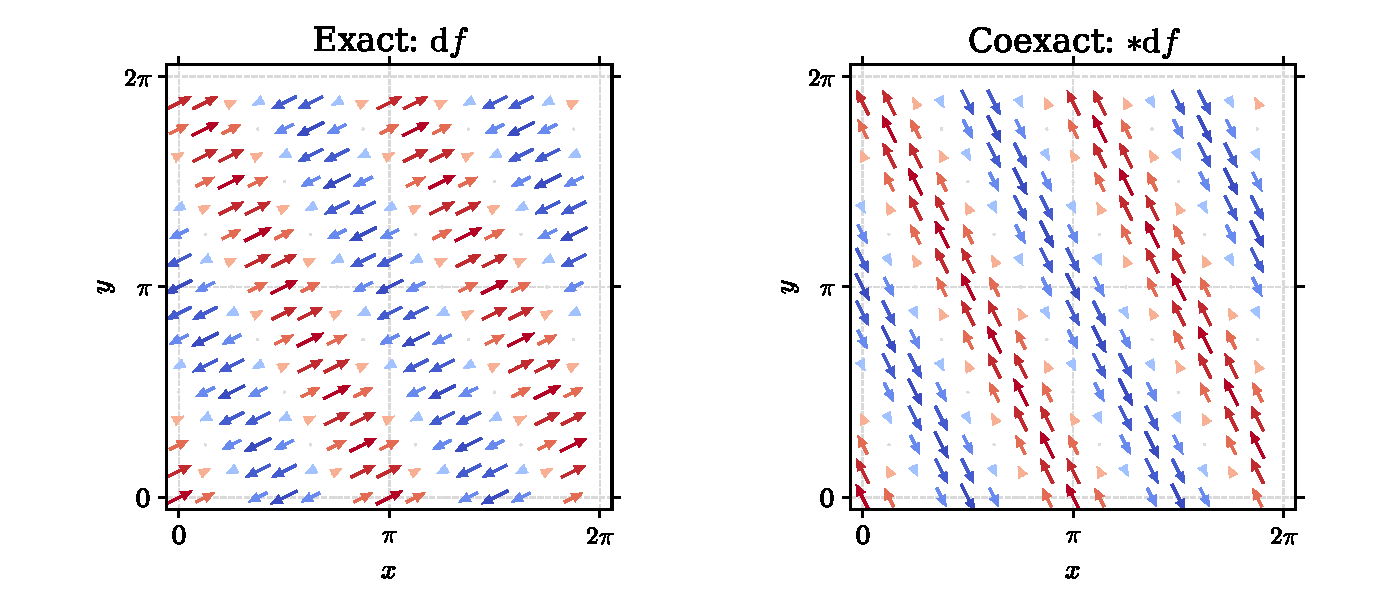
\includegraphics[width=.93\linewidth]{content/MathSkills/figures/geometry-highspin/torus_hodge_vector_modes.pdf}
\caption{\cref{eq:ghs-r9-torus-hodge-sample} 的恰当与余恰当一形式，在环面基本方域上的矢量场箭头。红色表示 $\cos(2x+y)>0$、蓝色表示 $\cos(2x+y)<0$，颜色强度反映其绝对值，两种模式的箭头方向始终正交；边界应按周期识别，不能把图中方域的四条边视为真实物理边界。}\label{fig:ghs-r9-hodge-vector-modes}
\end{figure}

图中的两组箭头采用相同的矢量幅度标尺，箭头长度正比于局部 $|\cos(2x+y)|$，方向和颜色共同标示符号；严格的模态范数仍应使用 $\int_{T^2}|\alpha|^2\dd\mu$。当背景是任意闭定向曲面 $\Sigma$ 时，Hodge 定理仍给出 $\alpha=\dd f+*\dd g+h$，但 $h$ 的维数改为 $2\operatorname{genus}(\Sigma)$，而且不再有简单的整数平面波标签。对有边界的曲面，还必须指定绝对或相对 Hodge 边界条件，才能谈正交分解与零模维数。

\subsection{Hodge、粗拉普拉斯与规范场边界变分}

外微分的幂零关系与联络的曲率作用共同确定一形式场方程，但二者承担不同的约束。

局部张量表示确定了场的分量，但没有确定哪些分量可以独立传播。对带规范冗余的场，还必须把几何上的微分恒等式与动力学约束同时处理。

标量场的谱只需要 $-\Delta$；带自旋的场却生活在非平凡向量丛中，微分算子必须体现联络及曲率。即使是自旋一，也存在至少两种常用的 拉普拉斯算子。若没有弄清楚两者的差别，就容易错误地把普通函数的球谐谱推广成矢量或张量谱。

在定向黎曼流形上，令 $\Omega^p(M)$ 是光滑 $p$ 形式空间，外微分 $\dd:\Omega^p\to\Omega^{p+1}$ 满足 $\dd^2=0$。取 Hodge 星算子 $*$ 与 $L^2$ 内积，外微分的形式伴随记为 $\delta$。这里 $\Delta_H$ 非负；前面的散度型标量算子 $\Delta_g=\operatorname{div}\operatorname{grad}$ 非正，两者在标量上满足 $\Delta_H=-\Delta_g$。在无边界紧致流形上有
\begin{equation}\label{eq:ghs-hodge-laplacian}
 \Delta_{\rm H}=\dd\delta+\delta\dd.
\end{equation}
$\Delta_{\rm H}$ 在 $p$ 形式上非负，因为
$\langle\Delta_{\rm H}\omega,\omega\rangle
 =\norm{\dd\omega}^2+\norm{\delta\omega}^2$。边界存在时这个公式还会出现边界项，故必须补充绝对或相对边界条件。

\begin{theorem}[Hodge 分解]
\label{thm:ghs-hodge-decomposition}
在紧致、无边界、光滑定向黎曼流形上，$L^2$ 的 $p$ 形式有正交分解
\begin{equation}\label{eq:ghs-hodge-direct-sum}
 L^2\Omega^p=\overline{\operatorname{im}\dd}
 \oplus\overline{\operatorname{im}\delta}\oplus\ker\Delta_{\rm H}.
\end{equation}
每个 de Rham 上同调类有唯一调和代表，故 $\dim\ker\Delta_{\rm H}=b_p(M)$，是拓扑不变量。
\end{theorem}
\begin{proof}
$\Delta_{\rm H}$ 是椭圆非负自伴算子，紧致性使其零本征空间有限维，且 Hilbert 空间按核与正谱正交分解。对正谱部分设 $G=\Delta_{\rm H}^{-1}$，则
\[
 \omega=\mathcal H\omega+\Delta_{\rm H}G(1-\mathcal H)\omega
 =\mathcal H\omega+\dd\delta G\omega+\delta\dd G\omega,
\]
$\mathcal H$ 是调和投影。$\dd^2=\delta^2=0$ 和积分分部说明后两个子空间正交；调和形式与它们也正交。若 $\omega$ 闭合，则 $\dd\omega=0$，上式中的余微分项为零，剩下 $\omega=\mathcal H\omega+\dd\alpha$，说明每个闭形式与唯一的调和形式同调。调和且恰当的形式由范数恒等式只能为零，所以代表唯一。
\end{proof}

这个结论对规范场特别重要：零模个数可以由空间拓扑决定，而不由局域曲率常数决定。例如环面上的一形式具有非平凡调和模式，二球上的一般一形式却没有相同的同调零模结构。

联络导出粗 拉普拉斯算子 $\nabla^*\nabla$。对一形式 $\omega_a$，Weitzenböck 恒等式为
\begin{equation}\label{eq:ghs-weitzenbock-one-form}
 (\Delta_{\rm H}\omega)_a=(\nabla^*\nabla\omega)_a
 +\operatorname{Ric}_a{}^b\omega_b.
\end{equation}
它表明曲率以代数势项的形式改变了自旋一的传播算子。对高阶张量也存在相应曲率作用，但不能只用标量曲率 $\mathcal R$ 乘单位矩阵代替全部 Riemann 张量缩并。

\begin{proof}[证明（一形式曲率项的计算）]
对一形式展开协变导数，并交换指标，可核对曲率项的系数。
取 $\delta\omega=-\nabla^a\omega_a$，则
\begin{align*}
(\dd\delta\omega)_b&=-\nabla_b\nabla^a\omega_a,\\
(\delta\dd\omega)_b&=-\nabla^a(\nabla_a\omega_b-\nabla_b\omega_a)\\
&=-\nabla^a\nabla_a\omega_b+\nabla^a\nabla_b\omega_a.
\end{align*}
相加后得到 $-\nabla^a\nabla_a\omega_b+[\nabla^a,\nabla_b]\omega_a$。按照前文固定的曲率约定，该对易项收缩为 $\operatorname{Ric}_b{}^a\omega_a$，于是得 \cref{eq:ghs-weitzenbock-one-form}。这是带自旋算子与标量 拉普拉斯算子的第一个明确差异。

\end{proof}

考虑 $U(1)$ 规范场 $A\in\Omega^1(M)$，曲率 $F=\dd A$，作用量 $\mathscr I[A]=\frac14\int F_{ab}F^{ab}\dd\mu_g=\frac12\norm{\dd A}^2$。规范变换 $A\mapsto A+\dd\alpha$ 不改变 $F$。在 Lorenz 型规范 $\delta A=0$ 下，形式动力学算子与 $\Delta_{\rm H}$ 密切相关。然而零模可能包括精确形式的纯规范方向，以及非精确调和一形式的全局模态；二者必须区别商掉。

若区域有边界，允许的 $\alpha$ 是在边界消失还是可取非零值，直接决定边界荷与 Hilbert 空间分解。不能仅由局域的自旋一张量表示得出规范场全部物理自由度。高自旋规范场也存在类似的约束、迹条件与背景曲率一致性问题。

对对称二张量 $h_{ab}$，取四指标排列 $R_{abcd}=g(R(e_a,e_b)e_c,e_d)$，并记 $R_a{}^c=\operatorname{Ric}_a{}^c$。可以构造一种二阶椭圆算子，其主符号部分是 $-\nabla^2h_{ab}$，曲率作用为
\begin{equation}\label{eq:ghs-lichnerowicz-two-tensor}
 (\Delta_{\rm L}h)_{ab}=-\nabla^c\nabla_ch_{ab}
 +R_a{}^ch_{cb}+R_b{}^ch_{ac}+2R_{acbd}h^{cd}.
\end{equation}
这里的四指标顺序与前面的 $R(X,Y,Z,W)$ 相同；若先降低 $R^a{}_{bcd}$ 的首指标，所得四指标张量等于本式 $R_{abcd}$ 的负值，曲率项便写成常见的 $-2$ 形式。
\begin{proof}[证明（度量张量的零模核对）]
由度规相容性，$\nabla g=0$。由 Ricci 定义与曲率反对称性，
\[
 g^{cd}R_{acbd}=-\operatorname{Ric}_{ab}.
\]
因此取 $h=g$ 时
\[
 (\Delta_{\rm L}g)_{ab}
 =0+\operatorname{Ric}_{ab}+\operatorname{Ric}_{ab}
 +2(-\operatorname{Ric}_{ab})=0.
\]
常截面曲率 $k$ 的直接代入也给出 $R_{acbd}=k(g_{cb}g_{ad}-g_{ab}g_{cd})$，故其收缩为 $-(d-1)kg_{ab}$，与同一 Ricci 定义相符。
\end{proof}
该算子经常出现在 Einstein 方程的线性化、引力子涨落与相关规范固定问题中。它与单独作用于每个分量的标量 拉普拉斯算子 不是同一个算子。

对于更高阶对称无迹张量，二阶算子的可能曲率修正更多；若还要求规范不变性、幺正性和正确约束传播，允许的背景与耦合受到额外限制。这说明“空间任意”与“自旋任意”是两个独立的推广目标，不能在不增加物理假设的情况下同时任意化。

前面的高自旋微分算子涉及协变导数对易子，但对自旋一场还存在更强的结构：规范变换并不要求曲率消失，它直接来自外微分的恒等式 $\dd^2=0$。这一事实提供了区分“曲率使平直表达式失效”和“曲率破坏规范对称性”的一个可完全算通的例子。

先在无边界紧致定向黎曼流形上讨论欧氏二次型。令实一形式 $A=A_a\dd x^a$ 为规范势，$F=\dd A$ 为二形式场强。由于 Levi--Civita 联络无挠，
\begin{equation}\label{eq:ghs-r9-maxwell-fieldstrength}
 F_{ab}=\nabla_aA_b-\nabla_bA_a
 =\partial_aA_b-\partial_bA_a.
\end{equation}
定义作用量 $S[A]=\tfrac12\int_X F\wedge *F=\tfrac14\int_XF_{ab}F^{ab}\dd\mu_g$。变分时 $\delta F=\dd(\delta A)$，对闭流形积分分部：
\begin{align*}
 \delta S
 &=\int_X\dd(\delta A)\wedge *F
 =\langle F,\dd(\delta A)\rangle_{L^2}\\
 &=\langle\delta F,\delta A\rangle_{L^2}.
\end{align*}
这里最后一个 $\delta$ 在 $\delta A$ 中是变分符号，在 $\delta F$ 中则表示余微分；二者的数学角色不同。Euler--Lagrange 方程为
\begin{equation}\label{eq:ghs-r9-maxwell-coexact-eom}
 \delta\dd A=0.
\end{equation}
对任意光滑标量 $\chi$，取 $A\mapsto A+\dd\chi$，由于 $\dd^2\chi=0$，场强和作用量都不变。这一证明对所有光滑黎曼背景成立，不要求 Ricci 曲率为零。

\begin{proposition}[规范场的一形式 Weitzenbock 恒等式]
\label{prop:ghs-r9-maxwell-weitzenbock}
对一形式 $A$，Hodge 拉普拉斯算子满足
\begin{equation}\label{eq:ghs-r9-maxwell-curvature-term}
 (\dd\delta+\delta\dd)A
 =\nabla^*\nabla A+\operatorname{Ric}(A).
\end{equation}
选取 Lorenz 型规范 $\delta A=0$ 后，自由 Maxwell 方程成为 $\Delta_HA=0$。因此在曲空间直接用粗 拉普拉斯算子 $\nabla^*\nabla$ 代替 $\Delta_H$ 会漏掉 Ricci 项；但该项不是外加的规范对称性破缺项，而是由微分复形决定的几何补偿。
\end{proposition}
\begin{proof}
取正定 Laplace 约定，$\delta A=-\nabla^bA_b$，以及 $F_{ba}=\nabla_bA_a-\nabla_aA_b$。于是
\begin{align*}
 (\delta\dd A)_a
 &=-\nabla^bF_{ba}\\
 &=-\nabla^b\nabla_bA_a+\nabla^b\nabla_aA_b.
\end{align*}
另一方面，$(\dd\delta A)_a=-\nabla_a\nabla^bA_b$，所以
\[
 (\Delta_HA)_a=-\nabla^b\nabla_bA_a
 +[\nabla^b,\nabla_a]A_b.
\]
按本书采用的 Ricci 曲率约定，最后的缩并交换子恰为 $\operatorname{Ric}_a{}^bA_b$。第一项是粗 拉普拉斯算子，这就得到了 \cref{eq:ghs-r9-maxwell-curvature-term}。对 $A=\dd\chi$，还可用 $\Delta_H\dd\chi=\dd\Delta_H\chi$ 检查 Ricci 项准确抵消粗 拉普拉斯算子 与梯度不交换的部分。
\end{proof}

这个推导也解释了矢量球谐中两个容易混用的本征值。单位二球若 $\Delta_HY_{\ell m}=\ell(\ell+1)Y_{\ell m}$，则对 $\ell\ge1$，
\[
 \Delta_H(\dd Y_{\ell m})=\ell(\ell+1)\dd Y_{\ell m},\qquad
 \nabla^*\nabla(\dd Y_{\ell m})=[\ell(\ell+1)-1]\dd Y_{\ell m}.
\]
差值恰是 $S^2$ 的 Ricci 本征值 $1$。在环面上 Ricci 为零，两算子则具有相同本征值。这是上述 Hodge 分解、曲率算子以及表示谱的同一个交叉检验，而不是三个互不相干的公式。

如果 $X$ 有边界，$\delta$ 是 $\dd$ 的形式伴随时会出现边界配对；选择绝对或相对边界条件不仅影响自伴性，也影响允许的规范参数与调和零模。即使无边界，零模 $h$ 满足 $\dd h=\delta h=0$ 时仍可出现在 $A$ 中，且不一定是全局的 $\dd\chi$。例如环面上的 $\dd x,\dd y$ 对应不可用单值周期规范函数消去的平坦连接；在耦合带电场时，还需进一步考察它们的整体 holonomy。

将作用量分部积分时保留边界项，可直接得到相应的条件。
设 $X$ 有光滑边界，$\mathbf n$ 为外法向。对紧支于边界附近但边界取值不一定为零的变分，Stokes 定理给出
\[
 \int_X\langle F,\dd(\delta A)\rangle\dd\mu
 =\int_X\langle\delta F,\delta A\rangle\dd\mu
 +\int_{\partial X}\mathbf n^aF_{ab}\,\delta A^b\dd\mu_{\partial X}.
\]
因此固定切向规范势（Dirichlet 型）时边界变分消失；若允许边界 $A$ 自由变化，则自然条件是相应切向分量的 $\mathbf n^aF_{ab}=0$。一般相对/绝对 Hodge 条件还需同时约束规范固定算子的域，不能只规定 $F$ 的一个分量便宣称椭圆自伴问题已经完全确定。边界上的规范变换还可能成为真实的边缘自由度，因而与无边界的情形存在物理差别。


\section{Killing 流与 Hodge 算子的相容性}

Killing 流保持 $g$。因为它从恒等映射连续生成，在局部还保持既定定向，所以同时保持 $\operatorname{vol}_g$。由 Hodge 星的刻画\eqnrefs{eq:math-dg-hodge-star-characterization}可知
\[
\Phi_t^*(*\alpha)=*(\Phi_t^*\alpha).
\]
对 $t=0$ 求导得到
\begin{equation*}[\mathcal L_X,*]=0.
\end{equation*}
再结合 $[\mathcal L_X,\dd]=0$，立即得到
\begin{equation*}[\mathcal L_X,\delta]=0,
\qquad
[\mathcal L_X,\Delta]=0.
\end{equation*}
因此 Hodge 拉普拉斯算子 的每个特征空间都在 Killing 对称下保持。几何对称与谱分解并不是两套独立技巧：它们可以在同一个不变子空间分解中同时使用。
Killing 方程和 Hodge 理论分别控制对称性与微分形式的分解。以下从度量内积与体积形式直接构造星算子、余微分和守恒量。

\section{等距流、Killing 场与守恒量}

有了联络和度量，便能严格表达“空间沿某方向移动后看起来不变”。
设向量场 \(K\) 的局部流为 \(\Phi_t\)：从点 \(p\) 出发，
曲线 \(t\mapsto\Phi_t(p)\) 满足
\(\frac{\dd}{\dd t}\Phi_t(p)=K_{\Phi_t(p)}\)、\(\Phi_0(p)=p\)。
如果流把度量保持不变，即
\(g_{\Phi_t(p)}(\dd\Phi_t X,\dd\Phi_t Y)=g_p(X,Y)\)，
就称 \(\Phi_t\) 为局部等距流。

\begin{definition}[Lie 导数与 Killing 场]
度量沿 \(K\) 的 Lie 导数定义为
\[
(\mathcal L_Kg)_p(X,Y)
=\left.\frac{\dd}{\dd t}\right|_{t=0}
(\Phi_t^*g)_p(X,Y).
\]
若 \(\mathcal L_Kg=0\)，称 \(K\) 为 Killing 场。
\end{definition}

这里 \(\Phi_t^*g\) 表示先用微分 \(\dd\Phi_t\)
把 \(p\) 处两个向量推到 \(\Phi_t(p)\)，再在那里计算 \(g\)。
所以定义不是“直接微分不同点的矩阵”，而是先把不同点的双线性型
拉回同一切空间再比较。

\begin{proposition}[Killing 方程]
对 Levi--Civita 联络，\(K\) 是 Killing 场当且仅当
\[
g(\nabla_XK,Y)+g(X,\nabla_YK)=0
\quad\text{对所有 }X,Y.
\]
在坐标中这等价于
\(\nabla_\mu K_\nu+\nabla_\nu K_\mu=0\)。
\end{proposition}
\begin{proof}
从流的定义对 \(t\) 求导，或在一张坐标图中直接对
\(g_{kl}(\Phi_t(x))\partial_i\Phi_t^k\partial_j\Phi_t^l\)
求导，得到
\[
(\mathcal L_Kg)(X,Y)
=K[g(X,Y)]-g([K,X],Y)-g(X,[K,Y]).
\]
度量相容性给
\(K[g(X,Y)]=g(\nabla_KX,Y)+g(X,\nabla_KY)\)。
无挠性给 \([K,X]=\nabla_KX-\nabla_XK\)，对 \(Y\) 亦然。
代入并约去 \(\nabla_KX,\nabla_KY\) 项，便得到命题中的式子。
\end{proof}

若 \(\gamma(t)\) 是仿射参数测地线，令 \(u=\dot\gamma\)，
则 \(\nabla_uu=0\)。因此
\[
\frac{\dd}{\dd t}g(K,u)
=g(\nabla_uK,u)+g(K,\nabla_uu)=0.
\]
第一项是 Killing 方程取 \(X=Y=u\) 的一半，第二项由
测地线方程消失。这给出守恒量 \(g(K,u)\)。
例如欧氏平面中 \(K=\partial_x\) 产生平移，
\(g(K,u)=\dot x\) 守恒；\(K=-y\partial_x+x\partial_y\)
产生旋转，\(g(K,u)=x\dot y-y\dot x\) 守恒。
由此可见“对称性给守恒量”不是额外的口号，而是度量相容性
与 Killing 方程的直接推论。


\par
\begin{workedexample}
对单位球面度量
\(g=\dd\vartheta^2+\sin^2\vartheta\,\dd\varphi^2\)，
用同一办法计算 \(\Delta_{\rm dR}f\)。
特别检验 \(f=\cos\vartheta\) 满足
\(\Delta_{\rm dR}f=2f\)。
\textbf{解.} 对函数，正号 Hodge--de Rham Laplacian 为负的 Laplace--Beltrami 算子：
\[
\Delta_{\rm dR}f=-\frac1{\sin\vartheta}\partial_\vartheta
(\sin\vartheta\,\partial_\vartheta f)
-\frac1{\sin^2\vartheta}\partial_\varphi^2f.
\]
令 \(f=\cos\vartheta\)，则 \(\partial_\vartheta f=-\sin\vartheta\)，角向散度项为 \(-2\cos\vartheta\)，再乘整体负号得 \(\Delta_{\rm dR}f=2\cos\vartheta=2f\)。
\end{workedexample}
\par
\section{Hodge 对偶从内积与体积形式定义}

上一章已把 \(k\)-形式定义为交替的 \(k\) 重协变张量。
现在先取定向的 \(n\) 维 Riemann 流形，即度量正定；
伪 Riemann 情形的符号稍后单独说明。
在每点选正向正交余标架 \(e^1,\ldots,e^n\)。
体积形式是
\(\mathrm{vol}_g=e^1\wedge\cdots\wedge e^n\)。
若 \(I=(i_1<\cdots<i_k)\)，记
\(e^I=e^{i_1}\wedge\cdots\wedge e^{i_k}\)，
规定这些 \(e^I\) 为 \(\Lambda^kT_p^*M\) 的正交归一基；
这将向量上的度量唯一延拓为 \(k\)-形式上的内积。

\begin{definition}[Hodge 星号]
Hodge 算子 \(*:\Lambda^kT_p^*M\to\Lambda^{n-k}T_p^*M\)
由对任意 \(k\)-形式 \(\alpha,\beta\) 成立的等式
\[
\alpha\wedge *\beta
=\langle\alpha,\beta\rangle\,\mathrm{vol}_g
\]
唯一确定。
\end{definition}

存在性并非显然。对基形式 \(e^I\)，令 \(I^c\) 是补指标组，
定义 \(*e^I=\operatorname{sgn}(I,I^c)e^{I^c}\)，
其中符号由
\(e^I\wedge e^{I^c}
=\operatorname{sgn}(I,I^c)\mathrm{vol}_g\) 决定。
这样 \(e^J\wedge *e^I=\delta_{IJ}\mathrm{vol}_g\)，
再由双线性即可得到定义式。若有另一算子满足同式，
它与此算子之差同所有基 \(e^I\) 作楔积都为零；
补基系数逐一为零，故唯一。

在三维欧氏空间的正向直角坐标下，
\[
*1=\dd x\wedge\dd y\wedge\dd z,
\quad *\dd x=\dd y\wedge\dd z,
\quad *(\dd x\wedge\dd y)=\dd z,
\quad *(\dd x\wedge\dd y\wedge\dd z)=1.
\]
再作一次星号时，两组指标交换经过 \(k(n-k)\) 次换位，因而
\begin{equation}
*^2\alpha=(-1)^{k(n-k)}\alpha
\qquad\bigl(\alpha\in\Lambda^kT_p^*M\bigr).
\label{eq:math-hodge-square}
\end{equation}
这条公式以正定度量为前提。若度量签名有 \(q\) 个负方向，
在常用的正向伪正交基约定下还要乘 \((-1)^q\)；
因此只说 \(*^2=\pm1\) 而不说明维数、形式次数和签名是不完整的。


\par
\begin{workedexample}
在二维欧氏空间的正向坐标中求 \(*\dd x\) 与 \(*\dd y\)，
并直接检验 \cref{eq:math-hodge-square} 对一形式给 \(*^2=-1\)。
\textbf{解.} 在正向正交余标架 \((\dd x,\dd y)\) 下，定义式给
\[
*\dd x=\dd y,\qquad *\dd y=-\dd x.
\]
因此 \(*^2\dd x=-\dd x\)、\(*^2\dd y=-\dd y\)，与 \(k=1,n=2\) 时 \((-1)^{k(n-k)}=-1\) 一致。
\end{workedexample}
\par
\section{余微分与最熟悉的 Laplace 算子}

对紧支撑的形式，定义全空间内积为
\((\alpha,\beta)=\int_M\alpha\wedge *\beta\)。
在无边界流形，或使边界项消失的边界条件下，
外微分 \(\dd:\Omega^{k-1}(M)\to\Omega^k(M)\)
的形式伴随记为 \(\delta:\Omega^k(M)\to\Omega^{k-1}(M)\)，即
\((\dd\alpha,\beta)=(\alpha,\delta\beta)\)。
先取支集包含在一张坐标图内的形式；普通的逐坐标分部积分
使全微分的积分为零。所得等式只涉及点处运算，
故在重叠坐标图上也相同。
注意乘积求导式
\(\dd(\alpha\wedge *\beta)
=\dd\alpha\wedge *\beta+(-1)^{k-1}\alpha\wedge\dd(*\beta)\)，
把全微分项的积分移到另一边，再用星号平方公式，得到
\[
\delta\beta=(-1)^{n(k+1)+1}*\dd *\beta
\quad\text{在 Riemann 度量下}.
\]
边界不消失时，必须额外写出边界积分，不能把形式伴随
直接称为具体 Hilbert 空间算子的伴随。

Laplace--de Rham 算子定义为
\(\Delta_{\rm dR}=\dd\delta+\delta\dd\)。
对零形式即函数 \(f\)，\(\delta f=0\)，故
\(\Delta_{\rm dR}f=\delta\dd f\)。
在欧氏直角坐标中
\(\dd f=\sum_i(\partial_i f)\dd x^i\)，
由上述伴随公式逐项算得
\[
\Delta_{\rm dR}f=-\sum_i\partial_i^2f.
\]
它是分析中非负的 Laplacian \(-\nabla^2\)，与物理教材
常写的 \(\nabla^2\) 只差一个符号约定。
这一例子同时说明，抽象的形式语言最终必须能退回熟悉的偏微分算子。

极坐标不是另一套定义，只是同一算子的另一种写法。
由正交余标架 \(e^1=\dd r,e^2=r\,\dd\varphi\) 有
\(*\dd r=r\,\dd\varphi\)、\(*\dd\varphi=-\dd r/r\)。因此
\[
*\dd f=r(\partial_r f)\,\dd\varphi
-\frac{\partial_\varphi f}{r}\,\dd r,
\quad
\dd*\dd f=\left[\partial_r(r\partial_r f)
+\frac1r\partial_\varphi^2f\right]\dd r\wedge\dd\varphi.
\]
因为体积形式是 \(r\,\dd r\wedge\dd\varphi\)，再用
\(\delta\dd f=-*\dd*\dd f\)，得
\[
\Delta_{\rm dR}f
=-\frac1r\partial_r(r\partial_r f)
-\frac1{r^2}\partial_\varphi^2f.
\]
如果误把 \(\dd\varphi\) 当成单位长度的一形式，
第二项就会少一个 \(r^{-2}\)；余标架的长度不能省略。

电磁学给出另一个直接检验。在三维欧氏空间，先用度量把向量场
\(V\) 变成一形式 \(V^\flat=g(V,\cdot)\)；
把磁场向量 \(\vb{B}\) 记成二形式
\(\mathcal B=*\vb{B}^\flat\)。
按前面的星号表，
\[
\mathcal B=B_x\,\dd y\wedge\dd z
+B_y\,\dd z\wedge\dd x+B_z\,\dd x\wedge\dd y,
\qquad
\dd\mathcal B=(\nabla\cdot\vb{B})\,\dd x\wedge\dd y\wedge\dd z.
\]
对电场一形式 \(\mathcal E=\vb{E}^\flat\) 同样逐项求导，
\(\dd\mathcal E=*(\nabla\times\vb{E})^\flat\)。
所以 Maxwell 的两条无源运动学方程
\(\nabla\cdot\vb{B}=0\)、
\(\nabla\times\vb{E}=-\partial_t\vb{B}\)
恰可写成
\[
\dd\mathcal B=0,
\qquad
\dd\mathcal E+\partial_t\mathcal B=0.
\]
外微分的 \(\dd^2=0\) 还解释了为何若局部写
\(\mathcal B=\dd\mathcal A\)，第一条方程自动成立；
上章的穿孔平面反例同时提醒，局部势的存在不自动保证
它能作为全局单值对象使用。






\section{度量、Killing 与 Hodge 的公式联系}
以下公式采用定向 Riemann 流形的 Hodge 星约定；余微分中的 $k$ 表示它所作用的微分形式次数。Koszul 公式把度量接到联络，Killing 方程则把度量接到流。
\begin{note}[公式之间的联系]
Levi--Civita 联络由 Koszul 公式唯一确定：
\[
\begin{aligned}
2g(\nabla_XY,Z)
={}&Xg(Y,Z)+Yg(Z,X)-Zg(X,Y)\\
&+g([X,Y],Z)-g([Y,Z],X)+g([Z,X],Y).
\end{aligned}
\]
坐标中
\[
\Gamma^k{}_{ij}
=\frac12g^{k\ell}
(\partial_i g_{j\ell}+\partial_j g_{i\ell}-\partial_\ell g_{ij}).
\]
Killing、散度与 Hodge 公式为
\begin{align*}
\mathcal L_Xg&=0,\\
\nabla_iX_j+\nabla_jX_i&=0,\\
\mathcal L_X\operatorname{vol}_g&=(\operatorname{div} X)\operatorname{vol}_g,\\
\operatorname{div} X&=-\delta X^\flat=*\dd*X^\flat,\\
\delta&=(-1)^{n(k+1)+1}*\dd*,\\
\Delta&=\dd\delta+\delta\dd.
\end{align*}
Hodge 分解见\eqnrefs{eq:math-dg-hodge-decomposition}。
\end{note}

\begin{proposition}[Killing 方程的协变表达]
在 Riemann 流形上，\[\mathcal L_Xg=0\quad\Longleftrightarrow\quad\nabla_iX_j+\nabla_jX_i=0.\]对 Killing 场，仿射参数测地线上的 $g(X,\dot\gamma)$ 恒定。
\end{proposition}

\begin{proof}
将 $\mathcal L_Xg$ 的定义用 Levi--Civita 联络改写，利用度量相容性和无挠性消去高阶项，得到一阶方程。

对任意向量场 $Y,Z$，Lie 导数定义给出
\begin{equation*}
 (\mathcal L_Xg)(Y,Z)
 =X[g(Y,Z)]-g([X,Y],Z)-g(Y,[X,Z]).
\end{equation*}
这是 Lie 导数的 Cartan 公式在 $(0,2)$ 张量上的特例：第一项是 $X$ 作用于张量值，后两项扣除 $Y,Z$ 自身被 $X$ 的流推动产生的变化。

Levi--Civita 联络满足 $\nabla g=0$，故
\begin{equation*}
 X[g(Y,Z)]
 =(\nabla_Xg)(Y,Z)+g(\nabla_XY,Z)+g(Y,\nabla_XZ)
 =g(\nabla_XY,Z)+g(Y,\nabla_XZ).
\end{equation*}
度量相容性 $\nabla g=0$ 是 Levi--Civita 联络的两条公理之一，几何意义是"协变微分保持内积"。

$\nabla$ 无挠给出 $[X,Y]=\nabla_XY-\nabla_YX$、$[X,Z]=\nabla_XZ-\nabla_ZX$。代入上面的 Lie 导数定义，
\begin{align*}
 (\mathcal L_Xg)(Y,Z)
 &=g(\nabla_XY,Z)+g(Y,\nabla_XZ)\\
 &\quad -g(\nabla_XY-\nabla_YX,Z)-g(Y,\nabla_XZ-\nabla_ZX).
\end{align*}
无挠性是 Levi--Civita 联络的另一条公理，把 Lie 括号这一纯微分拓扑对象用协变导数表达。

含 $\nabla_XY$ 与 $\nabla_XZ$ 的项相消，留下
\begin{equation*}
 (\mathcal L_Xg)(Y,Z)
 =g(\nabla_YX,Z)+g(Y,\nabla_ZX).
\end{equation*}
此式对任意 $Y,Z$ 成立。注意 $X$ 现在被 $\nabla$ 作用，而不是作用于别人——这是 Killing 方程为一阶 PDE 的关键。

取 $Y=\partial_i$、$Z=\partial_j$，$g(\partial_i,\partial_j)=g_{ij}$，$\nabla_{\partial_i}X$ 的 $j$ 分量为 $\nabla_iX^j$，故
\begin{equation*}
 (\mathcal L_Xg)_{ij}
 =g_{jk}\nabla_iX^k+g_{ik}\nabla_jX^k
 =\nabla_iX_j+\nabla_jX_i.
\end{equation*}
$\mathcal L_Xg=0$ 即给出
\begin{equation}\label{eq:math-dg-synthesis-killing-eq}
\boxed{\nabla_iX_j+\nabla_jX_i=0,}
\end{equation}
即\eqnrefs{eq:math-dg-synthesis-killing-eq}。这是一阶线性 PDE。
沿测地线计算 $\nabla_TT=0$ 及 Killing 方程，得到
\[
\frac{\dd}{\dd s}g(X,T)=g(\nabla_TX,T)=0.
\]
Killing 场的限制是测地线变分的 Jacobi 场。
沿每条径向测地线，$X$ 由 $X(p)$ 与 $\nabla X(p)$ 的初值唯一决定；
Killing 方程又要求 $\nabla X(p)$ 反对称。
故在连通流形上，其第一 jet 的可能维数至多为
$n+\binom n2=n(n+1)/2$，零初值由 Jacobi ODE 的唯一性给出零场。



典型例子。
\begin{itemize}
\item $\RR^n$：平移 $\partial_i$ 与旋转 $x^i\partial_j-x^j\partial_i$ 共 $n+n(n-1)/2=n(n+1)/2$ 个 Killing 场，达到最大维数。
\item $S^n$：$SO(n+1)$ 的 Lie 代数给出 $n(n+1)/2$ 个 Killing 场，对应球面的等距群。
\item $\HH^n$：$SO(n,1)$ 给出 $n(n+1)/2$ 个 Killing 场，双曲空间也是最大对称空间。
\item 一般 Riemann 流形：Killing 场维数 $<n(n+1)/2$，反映对称性的缺失。
\end{itemize}

Killing 场对应度量的连续对称，沿测地线产生守恒量 $J_X=g(X,\dot\gamma)$。在广义相对论中，Killing 场对应时空对称（如稳态时空的时间平移 $\partial_t$ 给出能量守恒、轴对称 $\partial_\phi$ 给出角动量守恒）。Noether 定理在几何语言下即"Killing 场 $\Rightarrow$ 测地线守恒量"。在经典力学中，$n(n+1)/2$ 维最大对称空间对应 $n$ 维自由粒子全部运动积分的存在性。
\end{proof}

\begin{proposition}[Hodge 拉普拉斯的椭圆主符号]
设 $\Delta_H=\dd\delta+\delta\dd$ 作用于 Riemann 流形的 $k$-形式。采用 $\partial_j\mapsto\ii\xi_j$，\[\sigma_2(\Delta_H)(\xi)=|\xi|_g^2\operatorname{id}_{\Lambda^kT_p^*M}.\]故 $\Delta_H$ 椭圆。
\end{proposition}

\begin{proof}
计算 $\Delta=\dd\delta+\delta\dd$ 的二阶主符号。$\dd$ 与 $\delta$ 的一阶主符号分别由外积与插入算子给出，二者复合后用 Cartan 恒等式 $\iota_{\xi^\sharp}(\xi\wedge\cdot)+\xi\wedge\iota_{\xi^\sharp}\cdot=|\xi|^2\,\cdot$ 化为 $|\xi|^2\id()$。

在点 $p$ 处取非零余向量 $\xi\in T_p^*M$。采用 $\partial_j\mapsto \ii\xi_j$ 的主符号约定，外微分与余微分的一阶主符号分别为
\begin{equation*}
\sigma_1(\dd)(\xi)=\ii\,\xi\wedge,
\qquad
\sigma_1(\delta)(\xi)=-\ii\,\iota_{\xi^\sharp}.
\end{equation*}
$\sigma_1(\dd)=\ii\,\xi\wedge$ 来自外微分对一形式 $\alpha$ 给 $\dd\alpha=\partial_i\alpha_j\,\dd x^i\wedge\dd x^j$，主项含一阶导数。$\sigma_1(\delta)=-\ii\,\iota_{\xi^\sharp}$ 来自余微分的 Hodge 星定义与 $\delta=\pm *\dd*$ 中 $*$ 不改变阶数。

因此二阶算子 $\Delta=\dd\delta+\delta\dd$ 的主符号为
\begin{equation*}
\begin{aligned}
\sigma_2(\Delta)(\xi)
&=\sigma_1(\dd)\sigma_1(\delta)+\sigma_1(\delta)\sigma_1(\dd)\\
&=(\ii\,\xi\wedge)(-\ii\,\iota_{\xi^\sharp})
+(-\ii\,\iota_{\xi^\sharp})(\ii\,\xi\wedge)\\
&=(\xi\wedge)\iota_{\xi^\sharp}
+\iota_{\xi^\sharp}(\xi\wedge).
\end{aligned}
\end{equation*}
两个 $\ii$ 与 $-\ii$ 相乘都给 $+1$，符号约定使最终结果为正。

对任意形式 $\alpha$，插入算子与外积满足
\begin{equation*}
\iota_{\xi^\sharp}(\xi\wedge\alpha)
=|\xi|_g^2\alpha
-\xi\wedge\iota_{\xi^\sharp}\alpha.
\end{equation*}
这是 Cartan 公式 $\mathcal L_{\xi^\sharp}=\dd\iota_{\xi^\sharp}+\iota_{\xi^\sharp}\dd$ 在常向量场上的特例，也可直接对单项式 $\alpha=\theta^{i_1}\wedge\cdots\wedge\theta^{i_k}$ 验证：若 $\xi$ 出现在 $\alpha$ 中，插入与外积相继给出 $|\xi|^2$；若不出现，外积先添加该方向，插入再移除，仍给出 $|\xi|^2\alpha$；两种情形都是同一个反对易恒等式。

把 Cartan 恒等式代入主符号表达式，
\begin{equation*}
\iota_{\xi^\sharp}(\xi\wedge\alpha)
+\xi\wedge\iota_{\xi^\sharp}\alpha
=|\xi|_g^2\alpha
-\xi\wedge\iota_{\xi^\sharp}\alpha
+\xi\wedge\iota_{\xi^\sharp}\alpha
=|\xi|_g^2\alpha,
\end{equation*}
两项相消，恰好得到
\begin{equation}\label{eq:math-dg-hodge-principal-symbol}
\boxed{
\sigma_2(\Delta)(\xi)
=|\xi|_g^2\id(\Lambda^kT_p^*M).}
\end{equation}
当 $\xi\neq0$ 时该线性映射可逆，故 $\Delta$ 是椭圆算子。结合\eqnrefs{eq:math-dg-hodge-energy}的非负性与适当自伴定义域，就能调用前面建立的自伴谱理论，而不必把 Hodge 分解当作孤立结论。

典型例子与对比。
\begin{itemize}
\item $\RR^n$ 上 $0$-形式（函数）：$\Delta f=-\sum_i\partial_i^2 f$（本书非负约定），主符号 $|\xi|^2$，正是普通 拉普拉斯算子。
\item $\RR^n$ 上 $1$-形式：$\Delta\alpha_j=-\sum_i\partial_i^2\alpha_j$，每个分量独立满足标量 拉普拉斯算子，主符号仍是 $|\xi|^2\id()$。
\item 一般流形：主符号与 $\RR^n$ 相同，但低阶项含曲率（见 Weitzenböck 公式 $\Delta_H=\nabla^*\nabla+\operatorname{Ric}$），曲率通过低阶项影响谱而非椭圆性。
\end{itemize}

Hodge 拉普拉斯算子 的椭圆性是 Hodge 定理成立的分析基础：椭圆 + 自伴 + 非负 + 紧致流形 $\Rightarrow$ 谱离散且有限维核。在物理中，紧致空间上经过适当规范固定的椭圆线性化具有有限维核；这不能直接推广为全部非线性规范场解空间有限维，以及弦理论中 拉普拉斯算子 谱决定物理态能级。Weitzenböck 公式把椭圆性 + 曲率正性结合，给出 Bochner 消没定理——曲率通过低阶项直接控制核空间维数。
\end{proof}

\begin{theorem}[Green 算子与 Hodge 分解]
在紧致、定向、无边界 Riemann 流形上，每个光滑 $k$-形式唯一分解为三个两两正交分量\[\alpha=\Pi_{\mathcal H,k}\alpha+\dd\delta\mathcal G_k\alpha+\delta\dd\mathcal G_k\alpha.\]每个 de Rham 类有唯一调和代表，两个势本身可不唯一。
\end{theorem}

\begin{proof}
在紧致无边界流形上，限制在 $\Omega^k(M)$ 的椭圆自伴算子记为 $\Delta_k$。它具有离散非负谱，零特征空间就是有限维的 $\mathcal H^k(M)$。记到该零空间的正交投影为 $\Pi_{\mathcal H,k}$，并在其正交补上定义 Green 算子
\[
\mathcal G_k:=\left(\Delta_k\big|_{\mathcal H^k(M)^\perp}\right)^{-1},
\qquad
\mathcal G_k\eta=0\quad(\eta\in\mathcal H^k(M)).
\]
于是谱分解给出精确算子恒等式
\[
I=\Pi_{\mathcal H,k}+\Delta_k\mathcal G_k.
\]
对任意 $\alpha\in\Omega^k(M)$，直接展开 $\Delta_k=\dd\delta+\delta\dd$ 得
\[
\begin{aligned}
\alpha
&=\Pi_{\mathcal H,k}\alpha+\Delta_k\mathcal G_k\alpha\\
&=\Pi_{\mathcal H,k}\alpha
+\dd\delta\mathcal G_k\alpha
+\delta\dd\mathcal G_k\alpha.
\end{aligned}
\]
令
\[
\alpha_{\mathcal H}=\Pi_{\mathcal H,k}\alpha,
\qquad
\beta=\delta\mathcal G_k\alpha,
\qquad
\gamma=\dd\mathcal G_k\alpha,
\]
便得到\eqnrefs{eq:math-dg-hodge-decomposition}。

三个分量两两正交。例如
\[
(\dd\beta,\delta\gamma)
=(\dd^2\beta,\gamma)=0,
\]
而对 调和 分量 $\alpha_{\mathcal H}$，由 $\dd\alpha_{\mathcal H}=\delta\alpha_{\mathcal H}=0$，
\[
(\dd\beta,\alpha_{\mathcal H})=(\beta,\delta\alpha_{\mathcal H})=0,
\qquad
(\delta\gamma,\alpha_{\mathcal H})=(\gamma,\dd\alpha_{\mathcal H})=0.
\]
因此三项本身唯一。若只改变 $\beta$ 为 $\beta+\zeta$ 且 $\dd\zeta=0$，精确 分量不变，所以势并不唯一；$\gamma$ 同理。

最后证明调和代表与 de Rham 上同调一一对应。调和形式由\eqnrefs{eq:math-dg-harmonic-closed-coclosed}必为闭形式，故定义上同调类。若 $\eta_1-\eta_2=\dd\zeta$ 且 $\eta_1,\eta_2$ 都 调和，则
\[
\|\eta_1-\eta_2\|^2
=(\eta_1-\eta_2,\dd\zeta)
=(\delta(\eta_1-\eta_2),\zeta)=0,
\]
所以同一上同调类至多一个 调和 代表。另一方面若 $\alpha$ 闭，Hodge 分解给出
\[
\alpha=\dd\beta+\delta\gamma+\alpha_{\mathcal H}.
\]
对两边作用 $\dd$，得到 $\dd\delta\gamma=0$。于是
\[
\|\delta\gamma\|^2
=(\gamma,\dd\delta\gamma)=0,
\]
故 $\delta\gamma=0$，从而 $[\alpha]=[\alpha_{\mathcal H}]$。存在性成立。
\end{proof}

\begin{theorem}[实 de Rham 上同调的 Poincaré 对偶]
设 $M^n$ 紧致、定向、无边界。配对\[H^k_{\mathrm{dR}}(M;\RR)\times H^{n-k}_{\mathrm{dR}}(M;\RR)\to\RR,\qquad([\alpha],[\beta])\mapsto\int_M\alpha\wedge\beta\]良定义且非退化，故 $b_k=b_{n-k}$。
\end{theorem}

\begin{proof}
先验证\eqnrefs{eq:math-dg-poincare-pairing}只依赖上同调类。若 $\alpha\mapsto\alpha+\dd\eta$ 且 $\beta$ 闭，则由 $\dd\beta=0$ 及外微分 Leibniz 律
\[
\dd(\eta\wedge\beta)
=\dd\eta\wedge\beta+(-1)^{\deg\eta}\eta\wedge\dd\beta
=\dd\eta\wedge\beta,
\]
故由 Stokes 定理及 $\partial M=\varnothing$，
\[
\int_M\dd\eta\wedge\beta
=\int_M\dd(\eta\wedge\beta)
=\int_{\partial M}\eta\wedge\beta
=0.
\]
对 $\beta$ 的 精确 改变 $\beta\mapsto\beta+\dd\zeta$ 同理，因 $\alpha$ 闭且
\[
\dd(\alpha\wedge\zeta)
=\dd\alpha\wedge\zeta+(-1)^{\deg\alpha}\alpha\wedge\dd\zeta
=(-1)^{\deg\alpha}\alpha\wedge\dd\zeta,
\]
故
\[
\int_M\alpha\wedge\dd\zeta
=(-1)^k\int_M\dd(\alpha\wedge\zeta)=0.
\]
因此配对在上同调上良定。

现在取非零上同调类 $[\alpha]\neq0$，并令 $h$ 为其唯一调和代表元，即 $\Delta h=0$。由\eqnrefs{eq:math-dg-hodge-star-harmonic-isomorphism}，Hodge 星保持 调和 性，故 $*h$ 也是 调和，因此定义一个 $(n-k)$ 次上同调类
\[
[*h]\in H^{n-k}_{\mathrm{dR}}(M).
\]
于是由 Hodge 星的定义\eqnrefs{eq:math-dg-hodge-star-characterization}，
\begin{align*}
\int_M h\wedge *h
&=\int_M \langle h,h\rangle_g\,\operatorname{vol}_g\\
&=\int_M |h|_g^2\,\operatorname{vol}_g\\
&=\|h\|_{L^2}^2.
\end{align*}
由 $[\alpha]\neq0$ 故 $h\neq0$，从而
\[
\|h\|_{L^2}^2>0.
\]
所以 $[\alpha]$ 与 $[*h]$ 配对非零，不可能与所有 $H^{n-k}_{\mathrm{dR}}(M)$ 元素配对为零。反向非退化性由 $**h=(-1)^{k(n-k)}h$ 完全相同地得到：对非零 $[\beta]\in H^{n-k}_{\mathrm{dR}}(M)$，取其 调和 代表元 $k$，则
\[
\int_M k\wedge *k=\|k\|_{L^2}^2>0,
\]
故 $[\beta]$ 与 $[*k]\in H^k_{\mathrm{dR}}(M)$ 配对非零。因此配对非退化，而有限维向量空间之间的非退化配对立刻给出
\[
\dim H^k_{\mathrm{dR}}(M)
=\dim H^{n-k}_{\mathrm{dR}}(M).
\]

紧曲面 $\Sigma_g$（亏格 $g$）满足 $b_0=b_2=1$、$b_1=2g$，因而 $b_k=b_{2-k}$ 逐次成立；中间次数 $k=1$ 是自对偶的。紧 3-流形如 $T^3$ 则有 $b_0=b_3=1$、$b_1=b_2=3$。Poincaré 对偶不仅是维数等式，还给出上积配对 $H^k\times H^{n-k}\to H^n\cong\mathbb R$ 的非退化性——这是相交理论的基础：$k$-形式与 $(n-k)$-形式的上积对应对偶子流形的相交数。
\end{proof}

\begin{proposition}[一形式的 Weitzenböck 公式]
对 Riemann 流形上的光滑一形式，\[(\Delta_H\alpha)_j=(\nabla^*\nabla\alpha)_j+\operatorname{Ric}_j{}^k\alpha_k.\]在紧致无边界且 $\operatorname{Ric}>0$ 时，每个调和一形式为零。
\end{proposition}

\begin{proof}
对 $1$-形式 $\alpha$，分别计算 $\delta\dd\alpha$ 与 $\dd\delta\alpha$ 的分量，相加后把"协变导数交换子"识别为 Ricci 曲率，得到 $\Delta_H=\nabla^*\nabla+\operatorname{Ric}$。

对 $1$-形式 $\alpha=\alpha_j\dd x^j$，采用
\begin{equation*}
(\dd\alpha)_{ij}
=\nabla_i\alpha_j-\nabla_j\alpha_i,
\qquad
\delta\alpha=-\nabla^i\alpha_i.
\end{equation*}
第一个是外微分的协变分量形式（无挠使 Christoffel 项相消），第二个是余微分的分量约定（散度的负号来自本书非负 拉普拉斯算子 约定）。

把 $\dd\alpha$ 视为 $2$-形式再作用 $\delta$：
\begin{equation*}
(\delta\dd\alpha)_j
=-\nabla^i(\dd\alpha)_{ij}
=-\nabla^i(\nabla_i\alpha_j-\nabla_j\alpha_i)
=-\nabla^i\nabla_i\alpha_j+\nabla^i\nabla_j\alpha_i.
\end{equation*}
第一项是非负约定的联络拉普拉斯 $\nabla^*\nabla$ 的主项，第二项保留待与 $\dd\delta\alpha$ 中的对应项合并。


\begin{equation*}
(\dd\delta\alpha)_j
=\nabla_j(\delta\alpha)
=-\nabla_j\nabla^i\alpha_i.
\end{equation*}
此处用了 $1$-形式 $\delta\alpha$ 的外微分分量公式 $(\dd f)_j=\nabla_j f$。

相加得到
\begin{equation*}
(\Delta_H\alpha)_j
=(\delta\dd\alpha+\dd\delta\alpha)_j
=-\nabla^i\nabla_i\alpha_j
+\nabla^i\nabla_j\alpha_i
-\nabla_j\nabla^i\alpha_i.
\end{equation*}
最后两项正是协变导数交换子。对协变 $1$-张量，
\begin{equation*}
(\nabla^i\nabla_j-\nabla_j\nabla^i)\alpha_i
=\operatorname{Ric}_j{}^k\alpha_k
\end{equation*}
（符号与本书前面的 Riemann 曲率 约定 相容）。这一识别来自 Riemann 曲率的分量定义 $[\nabla_a,\nabla_b]X^c=R^c{}_{dab}X^d$，对协变指标取 迹 给 Ricci：$R^i{}_{j i k}\alpha^k=\operatorname{Ric}_{jk}\alpha^k$。

另一方面，正规坐标中
\begin{equation*}
(\nabla^*\nabla\alpha)_j
=-\nabla^i\nabla_i\alpha_j
\end{equation*}
在基点成立，张量性使其全局成立，因此得到\eqnrefs{eq:math-dg-weitzenbock-oneform}。

典型例子与应用。
\begin{itemize}
\item $\RR^n$：$\operatorname{Ric}=0$，$\Delta_H=\nabla^*\nabla=-\sum_i\partial_i^2$，每个分量独立满足标量 拉普拉斯算子。
\item $S^n$（$n\ge2$，Ric $=(n-1)g$）：$\Delta_H=\nabla^*\nabla+(n-1)$。调和 $1$-形式满足 $\nabla^*\nabla\alpha=-(n-1)\alpha$，但 $\nabla^*\nabla$ 非负，故 $\alpha=0$，即 $H^1(S^n)=0$（$n\ge2$）。
\item 紧致流形 $\operatorname{Ric}>0$：Bochner 消没定理给 $H^1(M)=0$，结合 Bonnet--Myers 定理（$\operatorname{Ric}\ge(n-1)k>0$ $\Rightarrow$ 直径 $\le\pi/\sqrt{k}$）说明正 Ricci 曲率强烈限制流形拓扑。
\end{itemize}

对紧致、无边界的 Spin 流形，未扭曲 Dirac 算子满足
$D^2=\nabla^*\nabla+\mathrm{Scal}/4$。
若 $\mathrm{Scal}>0$，能量恒等式推出 $\ker D=0$。
在偶数维，进一步结合分次算子 $D^+$ 的 Atiyah--Singer 指标公式，
得到 $\operatorname{ind}(D^+)=\hat A(M)=0$。
若加入非平坦扭曲丛，平方中还有丛曲率项，不能只凭正标量曲率断言核为零。
热核的分次迹 $\operatorname{Str}(e^{-tD^2})$ 将局部曲率项与全局指标联系起来，
这一联系将在旋量章节的 Lichnerowicz 公式中继续展开。
\end{proof}

\begin{theorem}[Lichnerowicz 谱隙下界]
设 $(M^n,g)$ 紧致、连通、无边界，$n\ge2$，$\operatorname{Ric}\ge(n-1)kg$、$k>0$。非负函数拉普拉斯 $\Delta=-\Delta_{\mathrm{LB}}$ 的第一正本征值满足 $\lambda_1\ge nk$。
\end{theorem}

\begin{proof}
设 $(M^n,g)$ 紧致无边界，$\operatorname{Ric}\ge(n-1)kg$（$k>0$），$\Delta f=\lambda_1 f$（第一非零本征函数）。

对本征函数积分\eqnrefs{eq:math-dg-bochner-function}。紧致无边界时 Stokes 定理给出 $\int_M\Delta|\nabla f|^2\operatorname{vol}_g=0$（边界项消失），于是
\begin{equation*}
 0
 =\lambda_1\int_M|\nabla f|^2\operatorname{vol}_g
 -\int_M|\nabla^2f|^2\operatorname{vol}_g
 -\int_M\operatorname{Ric}(\nabla f,\nabla f)\operatorname{vol}_g.
\end{equation*}

由 Green 公式，
\begin{equation*}
 \int_M|\nabla f|^2\operatorname{vol}_g
 =\int_M f\,\Delta f\,\operatorname{vol}_g
 =\lambda_1\int_M f^2\operatorname{vol}_g.
\end{equation*}

由 Cauchy--Schwarz 不等式对 Hessian 的迹，
\begin{equation*}
 |\nabla^2 f|^2\ge\frac{1}{n}(\tr\nabla^2f)^2
 =\frac{1}{n}(\Delta f)^2
 =\frac{\lambda_1^2}{n}f^2.
\end{equation*}
由 Ricci 下界假设，
\begin{equation*}
 \operatorname{Ric}(\nabla f,\nabla f)\ge(n-1)k\,|\nabla f|^2.
\end{equation*}

这里只能在积分以后使用
$\int|\nabla f|^2=\lambda_1\int f^2$，点态恒等式 $|\nabla f|^2=\lambda_1f^2$ 不成立。
将两个下界代入上面的 Bochner 恒等式（移项后右端 $\ge0$）：
\begin{align*}
 0
 &\le \lambda_1^2\int_Mf^2\operatorname{vol}_g
  -\frac{\lambda_1^2}{n}\int_Mf^2\operatorname{vol}_g
  -(n-1)k\lambda_1\int_Mf^2\operatorname{vol}_g\\
 &=\lambda_1\left(\frac{(n-1)\lambda_1}{n}-(n-1)k\right)\int_Mf^2\operatorname{vol}_g\\
 &=(n-1)\lambda_1\left(\frac{\lambda_1}{n}-k\right)\int_Mf^2\operatorname{vol}_g.
\end{align*}

因为 $\lambda_1>0$（非常数本征函数）、$n>1$、$f\not\equiv0$，积分因子为正，故 $\lambda_1/n-k\ge0$，即 $\lambda_1\ge nk$。这就是\eqnrefs{eq:math-dg-lichnerowicz-gap}。

Lichnerowicz 下界与 Bonnet--Myers 直径上界 $\operatorname{diam}(M)\le\pi/\sqrt{k}$ 假设完全相同（$\operatorname{Ric}\ge(n-1)kg$），但结论从"直径有限"变成"拉普拉斯算子 的第一个正本征值远离零"。同一个 Ricci 下界同时约束几何尺度与低频谱。
\end{proof}

\begin{proposition}[Hodge 边界条件的 Green 能量恒等式]
设 $M$ 紧致、定向且有光滑边界。绝对条件 $\iota_\nu\omega=\iota_\nu\dd\omega=0$ 或相对条件 $j^*\omega=j^*\delta\omega=0$ 均推出\[(\Delta_H\omega,\omega)=\|\dd\omega\|^2+\|\delta\omega\|^2.\]调和零模闭且余闭，Hodge 星给出 $\mathcal H_A^k\cong\mathcal H_R^{n-k}$。
\end{proposition}

\begin{proof}
设 $M$ 为紧致、定向的 Riemann 流形，边界光滑，$\nu$ 为外法单位向量。
先对实微分形式计算；复形式在第二槽取共轭，结论相同。
对 $\alpha\in\Omega^{k-1}(M)$、$\beta\in\Omega^k(M)$，外微分乘积规则给出
\[
\dd(\alpha\wedge *\beta)
=\dd\alpha\wedge *\beta+(-1)^{k-1}\alpha\wedge\dd(*\beta).
\]
按正文的余微分约定，第二项积分为 $-(\alpha,\delta\beta)$。
Stokes 定理因而给出
\[
(\dd\alpha,\beta)-(\alpha,\delta\beta)
=\int_{\partial M}j^*(\alpha\wedge *\beta)
=\int_{\partial M}\langle\alpha,\iota_\nu\beta\rangle\,\dd S.
\]
最后一个等号可在正交余标架 $(\nu^\flat,\theta^1,\dots)$ 中验证：
只有 $\beta$ 的法向分量与 $\alpha$ 的切向分量参与边界积分。

对 $\Delta\omega=\delta\dd\omega+\dd\delta\omega$ 分别使用上式，得
\begin{align*}
(\delta\dd\omega,\omega)
&=\|\dd\omega\|^2-
\int_{\partial M}\langle\omega,\iota_\nu\dd\omega\rangle\,\dd S,\\
(\dd\delta\omega,\omega)
&=\|\delta\omega\|^2+
\int_{\partial M}\langle\delta\omega,\iota_\nu\omega\rangle\,\dd S.
\end{align*}
绝对条件 $\iota_\nu\omega=0$、$\iota_\nu\dd\omega=0$
逐项消去边界积分。相对条件 $j^*\omega=0$、$j^*\delta\omega=0$
则消去其中的切向因子。故两种域都满足
\[
(\Delta\omega,\omega)=\|\dd\omega\|^2+\|\delta\omega\|^2.
\]
若 $\Delta\omega=0$，两项非负，必有 $\dd\omega=\delta\omega=0$。
能量恒等式证明非负性和零模的闭、余闭性质；完整自伴性还使用
Hodge--Morrey--Friedrichs 的椭圆边界理论，不能只由一次分部积分宣称已经证明。

Hodge 星的点态恒等式
\[
\iota_\nu(*\omega)=*(\omega\wedge\nu^\flat),\qquad
**\omega=(-1)^{k(n-k)}\omega
\]
说明它交换切向和法向分量。再利用 $\delta*=\pm*\dd$，
绝对条件的两条式子变为 $j^*(*\omega)=0$、$j^*\delta(*\omega)=0$。
因此 $*:\mathcal H_A^k\to\mathcal H_R^{n-k}$ 是同构。

区间上的 $0$-形式使两种条件完全可见：绝对条件为
$f'(0)=f'(1)=0$，相对条件为 $f(0)=f(1)=0$。
$-f''=0$ 的 Neumann 解是常数，而 Dirichlet 解只有零。
相应地，$H^0([0,1])=\RR$、$H^0([0,1],\partial[0,1])=0$。

在乘积平坦度量的圆柱 $S^1\times[0,1]$ 上，$\dd\theta$ 是绝对调和
$1$-形式，$\dd t$ 是相对调和 $1$-形式。两种空间维数都为一，
但选出的代表不同；维数不能被写成必然不同。
圆盘以及半球同胚于闭球 $D^n$，其上同调为
\[
H^k(D^n)=
\begin{cases}\RR,&k=0,\\0,&k>0,\end{cases}
\qquad
H^k(D^n,\partial D^n)=
\begin{cases}\RR,&k=n,\\0,&k\ne n.\end{cases}
\]
特别地 $H^1(D^2,\partial D^2)=0$，非平凡相对类在次数 $2$，
由体积形式代表。半球的普通上同调不能等同于整个球面 $S^n$ 的上同调。
这些结果也可由可缩性、对偶定理与配对长正合列分别核对。

无边界时两种域重合，恢复通常的 Hodge 分解。
非定向的 Möbius 带则需要取向线丛：Hodge 星把普通形式映为取向扭曲的形式，
也可以在可定向二重覆盖上施加正确的奇偶条件，不能忽略该变换的类型。
\end{proof}


\chapter{Frobenius 定理：从分布到积分叶} \label{chap:math-geometric-structures}

向量场给出“允许运动的方向”，但给定若干方向并不保证它们真能拼成低维子流形。例如在三维空间中，每点选一个二维平面场，这些平面可能像螺旋一样彼此扭转，因而不存在处处与它们相切的曲面。Frobenius 定理精确回答可积性问题：一个常秩分布局部来自子流形，当且仅当它在 Lie 括号下闭合；用余切语言说，当且仅当它的湮灭一形式生成的微分理想在 $\dd$ 下闭合。

\section{分布、积分流形与 involutivity}

\begin{workedexample}[不可积的平面分布]
在 \(\mathbb R^3\) 上令 \(\alpha=\dd z-x\dd y\)，并令二维分布 \(D=\ker\alpha\)。判断它能否在每一点附近成为某族曲面的切平面。

\textbf{解。} 向量场 \(X=\partial_x\)、\(Y=\partial_y+x\partial_z\) 都满足 \(\alpha(X)=\alpha(Y)=0\)，且处处线性无关，因而张成 \(D\)。由交换子的定义，
\[
[X,Y]f=X(Yf)-Y(Xf)=\partial_z f,\qquad [X,Y]=\partial_z.
\]
但 \(\alpha(\partial_z)=1\)，所以交换子不属于 \(D\)。若 \(D\) 是曲面的切平面，沿曲面切向量场的交换子仍必须切于曲面，矛盾。等价地，\(\dd\alpha=-\dd x\wedge\dd y\) 且 \(\alpha\wedge\dd\alpha=-\dd z\wedge\dd x\wedge\dd y\ne0\)，违背 Frobenius 条件。
\end{workedexample}


秩为 $k$ 的光滑分布是切丛的秩 $k$ 光滑子丛
\[
\mathcal D\subset TM.
\]
局部可以选光滑向量场 $X_1,\ldots,X_k$ 使
\[
\mathcal D_p
=\operatorname{span}\{X_1(p),\ldots,X_k(p)\}.
\]
若存在浸入的 $k$ 维子流形 $L\subset M$，满足每点
\[
T_pL=\mathcal D_p,
\qquad p\in L,
\]
则称 $L$ 为 $\mathcal D$ 的积分流形。若每一点附近都能由这样的积分流形形成局部叶层，则称 $\mathcal D$ 可积。

分布称为 对合的，若任意局部截面 $X,Y\in\Gamma(\mathcal D)$ 都满足
\begin{equation}\label{eq:math-dg-frobenius-involutive}
[X,Y]\in\Gamma(\mathcal D).
\end{equation}
这个条件完全由光滑结构决定，不需要联络或度量。

\begin{theorem}[Frobenius 定理]\label{thm:math-dg-frobenius}
设 $\mathcal D\subset TM$ 是常秩 $k$ 的光滑分布。以下条件在局部等价：
\begin{enumerate}[label=(\roman*)]
\item $\mathcal D$ 可积；
\item $\mathcal D$ 对合的，即满足\eqnrefs{eq:math-dg-frobenius-involutive}；
\item 每点附近存在坐标 $(y^1,\ldots,y^n)$，使
\[
\mathcal D
=\operatorname{span}\{\partial_{y^1},\ldots,\partial_{y^k}\};
\]
\item 若 $\alpha^1,\ldots,\alpha^{n-k}$ 是湮灭丛
\[
\mathcal D^\circ
:=\{\alpha\in T^*M:\alpha|_{\mathcal D}=0\}
\]
的一组局部标架，则存在一形式 $\eta^a{}_b$ 使
\begin{equation}\label{eq:math-dg-frobenius-pfaff}
\dd\alpha^a=\eta^a{}_b\wedge\alpha^b.
\end{equation}
\end{enumerate}
\end{theorem}

从 (iii) 到 (i) 是直接的：固定 $y^{k+1},\ldots,y^n$ 即得到积分叶。从 (i) 到 (ii) 也立即成立，因为切于同一子流形的向量场的 Lie 括号仍切于该子流形。真正困难的是由括号闭合构造适配坐标。

\section{微分理想与 Pfaff 形式}

向量场版本的 involutivity 可以完全转写到余切空间。若 $\alpha\in\Gamma(\mathcal D^\circ)$ 且 $X,Y\in\Gamma(\mathcal D)$，则
\[
\alpha(X)=\alpha(Y)=0.
\]
外微分公式给出
\begin{equation}\label{eq:math-dg-frobenius-dalpha-bracket}
\dd\alpha(X,Y)
=-\alpha([X,Y]).
\end{equation}
因此 $[X,Y]\in\mathcal D$ 当且仅当每个湮灭一形式的 $\dd\alpha$ 在两个 $\mathcal D$ 方向上都为零。在线性代数上，这等价于 $\dd\alpha$ 至少含一个来自 $\mathcal D^\circ$ 的因子，从而得到\eqnrefs{eq:math-dg-frobenius-pfaff}。

若余维为一，$\mathcal D=\ker\alpha$ 且 $\alpha$ 处处非零，Frobenius 条件进一步压缩成
\begin{equation}\label{eq:math-dg-frobenius-codim-one}
\boxed{\alpha\wedge\dd\alpha=0.}
\end{equation}


\par
\begin{workedexample}
在 \(\RR^3\) 中考虑一形式
\[
\alpha=\dd z-x\,\dd y.
\]
求 \(\alpha\wedge\dd\alpha\)，据此判断 \(\ker\alpha\) 是否可积。再自行构造一个非零一形式 \(\widetilde\alpha\) 使 \(\widetilde\alpha\wedge\dd\widetilde\alpha=0\)，并写出其局部积分曲面。
\textbf{解。} \(\dd\alpha=-\dd x\wedge\dd y\)，所以
\[
\alpha\wedge\dd\alpha=(\dd z-x\,\dd y)\wedge(-\dd x\wedge\dd y)
=-\dd z\wedge\dd x\wedge\dd y\ne0,
\]
故 \(\ker\alpha\) 不可积。可取 \(\widetilde\alpha=\dd z\)，它非零且闭，因此 \(\widetilde\alpha\wedge\dd\widetilde\alpha=0\)；积分曲面为 \(z=C\)。
\end{workedexample}
\par

\begin{exbox}[接触型平面场不可积]
在 $\RR^3$ 上取
\[
\alpha=\dd z-x\,\dd y,
\qquad
\mathcal D=\ker\alpha.
\]
有
\[
\dd\alpha=-\dd x\wedge\dd y,
\]
因此
\[
\alpha\wedge\dd\alpha
=-(\dd z-x\dd y)\wedge\dd x\wedge\dd y
=-\dd z\wedge\dd x\wedge\dd y\neq0.
\]
所以 $\mathcal D$ 不可积：不存在处处以这些二维平面为切平面的曲面族。这一例子说明“每点都给出一个二维平面”远不足以保证它们能拼成曲面。
\end{exbox}

余维一 Pfaff 条件的另一端不是“稍微不可积”，而是一个非常刚性的极大不可积结构。设 $M^{2m+1}$ 为奇数维流形，若一形式 $\alpha$ 满足
\begin{equation}
\boxed{
\alpha\wedge(\dd\alpha)^m\neq0
\quad\text{处处成立},
}
\label{eq:math-dg-contact-condition}
\end{equation}
则称 $\alpha$ 为 接触形式，超平面分布
\[
\mathcal H:=\ker\alpha
\]
称为 接触 分布。条件\eqnrefs{eq:math-dg-contact-condition}立刻说明 $\mathcal H$ 不可能满足 Frobenius：若 $\dd\alpha=\eta\wedge\alpha$，则 $(\dd\alpha)^m$ 每一项都含 $\alpha$ 因子，从而 $\alpha\wedge(\dd\alpha)^m=0$，与接触条件矛盾。

更精确地，$\dd\alpha$ 在 $\mathcal H$ 上是非退化二形式。若 $X\in\mathcal H_p$ 且
\[
\dd\alpha_p(X,Y)=0
\qquad\forall Y\in\mathcal H_p,
\]
则由线性代数可推出 $X=0$。因此每个 接触 hyperplane 自身携带一个 $2m$ 维 辛 向量空间 结构
\begin{equation*}\left(\mathcal H_p,\dd\alpha_p|_{\mathcal H_p}\right).\end{equation*}
这说明 接触几何 可以看成“奇数维流形上随点变化的一族 辛 超平面”。

接触形式 还唯一确定一个横向向量场，称为 Reeb 矢量场 $R_\alpha$：
\begin{equation*}\boxed{
\alpha(R_\alpha)=1,
\qquad
\iota_{R_\alpha}\dd\alpha=0.
}\end{equation*}
存在唯一性来自分解
\[
T_pM=\mathcal H_p\oplus\RR R_\alpha(p).
\]
第一条件固定横向分量，第二条件利用 $\dd\alpha|_{\mathcal H}$ 的非退化性消除任何可能的水平修正。

Contact 分布 括号-生成 的充要条件由此给出：经反复 Lie 括号 后张成整个切空间（\eqnrefs{eq:math-dg-contact-step-two-bracket-generating}）。

这个现象与 Frobenius 恰好相反。Frobenius 条件要求 Lie 括号 不产生新方向，于是运动被困在低维叶片中；括号-生成 条件则要求反复 Lie 括号 最终张成整个切空间。Chow--Rashevskii 定理说明，在连通流形上若一个光滑分布 括号 生成，则任意两点都可由分段光滑的水平曲线连接。若再在 $\mathcal H$ 上给定内积，便得到 sub-Riemann 几何：距离只计算水平曲线长度，而“缺失方向”由非交换运动间接产生。

最基本的局部标准型由 接触 Darboux 定理 给出。任一点附近都存在坐标
\[
(q^1,\ldots,q^m,p_1,\ldots,p_m,z)
\]
使 接触形式 在乘以一个处处非零函数后可写成
\begin{equation*}\alpha
=\dd z-\sum_{a=1}^m p_a\,\dd q^a.\end{equation*}
因此 接触几何 与 辛几何 一样没有局部标量曲率型不变量：所有 接触 结构 在足够小邻域内都有相同标准形，真正的信息主要来自全局拓扑、Reeb 动力学 与附加结构。

接触形式 还可以通过增加一个实坐标变成真正的 辛形式。令
\[
\widetilde M:=\RR_s\times M,
\qquad
\lambda:=\ee^s\alpha,
\]
并定义
\begin{equation}
\boxed{
\omega:=\dd\lambda
=\ee^s(\dd s\wedge\alpha+\dd\alpha).
}
\label{eq:math-dg-contact-symplectization}
\end{equation}
由 $\dd^2=0$ 有 $\dd\omega=0$。更重要的是
\begin{align*}
\omega^{m+1}
&=(m+1)\ee^{(m+1)s}
\dd s\wedge\alpha\wedge(\dd\alpha)^m,
\end{align*}
由 接触 条件处处非零。因此 $\omega$ 非退化，$(\RR\times M,\omega)$ 是 辛 流形，称为 $(M,\alpha)$ 的 辛化。接触几何 因而不是与 辛几何 平行的孤立理论，而是奇数维边界数据在增加一个尺度方向后的偶数维 辛 几何。

向量场 $\partial_s$ 是这个 精确 辛 流形 的 Liouville 矢量场，因为
\begin{equation*}\iota_{\partial_s}\omega
=\ee^s\alpha=\lambda,
\qquad
\mathcal L_{\partial_s}\omega=\omega.\end{equation*}
所以沿 $s$ 方向平移会把 辛形式 作指数缩放。另一方面，Reeb 场在 辛化 中恰好由径向 Hamiltonian 识别：若
\[
H(s,x)=\ee^s,
\]
并采用 Hamiltonian 约定
\[
\iota_{X_H}\omega=-\dd H,
\]
则
\begin{equation*}X_H=R_\alpha.\end{equation*}
因为
\[
\iota_{R_\alpha}\omega
=\ee^s\iota_{R_\alpha}(\dd s\wedge\alpha+\dd\alpha)
=-\ee^s\dd s
=-\dd(\ee^s).
\]
这给 Reeb 动力学 一个非常具体的解释：它是在 辛化 上由纯尺度 Hamiltonian 产生的 Hamilton 流。

在 接触 流形 本身，也可为任意光滑函数 $H\in C^\infty(M)$ 定义 接触 Hamiltonian 矢量场 $X_H$。固定约定
\begin{equation}
\boxed{
\alpha(X_H)=H,
\qquad
\iota_{X_H}\dd\alpha
=(R_\alpha H)\alpha-\dd H.
}
\label{eq:math-dg-contact-hamiltonian}
\end{equation}
第二式在 $\mathcal H$ 上唯一确定 $X_H$ 的水平分量，第一式再确定 Reeb 分量。由 Cartan 公式立刻得到
\begin{equation*}\boxed{
\mathcal L_{X_H}\alpha
=(R_\alpha H)\alpha.
}\end{equation*}
因此 接触 Hamiltonian 流 一般不保持具体的一形式 $\alpha$，而保持其 核 所定义的 接触 分布；当 $R_\alpha H=0$ 时才严格保持 $\alpha$。

Hamilton 向量场的 接触 lift 由此确定为 $a=-R_\alpha H$（\eqnrefs{eq:math-dg-contact-hamiltonian-lift}）。

\begin{exbox}[三维 Heisenberg 接触 结构]
在 $\RR^3_{(x,y,z)}$ 上取
\[
\alpha=\dd z-\frac12(x\,\dd y-y\,\dd x).
\]
则
\[
\dd\alpha=-\dd x\wedge\dd y,
\qquad
\alpha\wedge\dd\alpha=-\dd z\wedge\dd x\wedge\dd y\neq0.
\]
一组水平向量场可取
\[
X=\partial_x-\frac y2\partial_z,
\qquad
Y=\partial_y+\frac x2\partial_z,
\]
而 Reeb 场为 $R_\alpha=\partial_z$。直接计算
\[
[X,Y]=\partial_z=R_\alpha.
\]
所以被禁止的竖直方向恰由两个水平运动的交换子生成。这是 Heisenberg 群、非完整约束与 sub-Riemann 控制理论共同的局部模型。
\end{exbox}

\subsection{正则叶片与适配度规}

可积分布给出局部叶片以后，度规还须确定法向距离、切向重标记与积分测度。

\begin{definition}[正则叶状分解]
\label{def:ghs-regular-foliation}
设 $U\subset M$ 是开区域，$I\subset\RR$ 是区间，$\Sigma$ 是 $(d-1)$ 维流形。若存在微分同胚 $F:I\times\Sigma\longrightarrow U$，则 $\Sigma_t=F(\{t\}\times\Sigma)$ 称为一族正则叶。函数 $t:U\to I$ 在每点满足 $\dd t\neq 0$，因此每个 $\Sigma_t$ 都是正则超曲面。
\end{definition}

此定义的用处是将“量子化面”与特定的球面分开。譬如平直空间去掉原点后有 $U\simeq\RR\times S^{d-1}$；而一般紧致流形可以没有全局非临界实函数，因此不存在这样的全局展开。临界点、拓扑变化与边界必须另行处理，不能一律塞进所谓的径向时间。

\begin{proposition}[叶状度规的分解]
\label{prop:ghs-foliation-metric}
在 $I\times\Sigma$ 上任取适配坐标 $(t,y^a)$，正定度规唯一写成
\begin{equation}\label{eq:ghs-foliation-adm}
 g=N^2\dd t^2+h_{ab}(\dd y^a+N^a\dd t)(\dd y^b+N^b\dd t),
\end{equation}
其中 $N>0$ 是 法向进动系数，$N^a$ 是 切向位移，$h_{ab}$ 是 $\Sigma_t$ 上的诱导度规。体积测度为
\begin{equation}\label{eq:ghs-foliation-volume}
 \dd\mu_g=N\sqrt{h}\,\dd t\,\dd^{d-1}y.
\end{equation}
\end{proposition}
\begin{proof}
按 $t$ 和 $y$ 分块写度规矩阵。由于 $h_{ab}$ 正定可逆，令 $N_a=g_{ta}$、$N^a=h^{ab}N_b$，再令 $N^2=g_{tt}-h^{ab}N_aN_b$。正定性和 Schur 补定理给出 $N^2>0$。展开 \cref{eq:ghs-foliation-adm} 得到原矩阵全部分量。分块行列式公式
\[
 \det g=\det h\,(g_{tt}-N_ah^{ab}N_b)=N^2\det h
\]
便证明测度公式。唯一性来自矩阵分块分解的唯一性。
\end{proof}

把 $t$ 增加 $\dd t$ 时，坐标向量 $\partial_t$ 一般不是单位法向。单位法向和法向微分为
\[
 n=N^{-1}(\partial_t-N^a\partial_a),\qquad
 \nabla_n\varphi=N^{-1}(\partial_t-N^a\partial_a)\varphi.
\]
这决定了标量场在两片叶之间真正改变了多少。不能在存在 切向位移 时仅用 $\partial_t\varphi$ 作为正交时间导数。


\section{从局部可积到全局叶空间：holonomy 与主丛水平分布}

Frobenius 定理是局部定理。若 $\mathcal D$ 对合的，通过每一点的局部积分流形可以沿重叠区域唯一延拓，并得到一个极大的连通积分叶；这些极大叶组成 foliation $\mathcal F$。但“每点都有局部叶”并不保证商空间
\[
 M/\mathcal F
\]
本身是流形，甚至不保证 Hausdorff。全局问题取决于叶的闭性、和乐 以及叶在 $M$ 中的回返方式，而这些信息都不包含在点态条件 $[X,Y]\in\Gamma(\mathcal D)$ 中。

最简单的反例是二维环面上的 Kronecker foliation。取
\[
 M=\mathbb T^2=\mathbb R^2/(2\pi\mathbb Z)^2,
 \qquad
 X=\partial_x+\alpha\partial_y,
 \qquad
 \alpha\notin\mathbb Q,
\]
并令 $\mathcal D=\operatorname{span}\{X\}$。秩一分布自动 对合的，因此每条积分曲线
\[
 t\longmapsto
 (x_0+t,\,y_0+\alpha t)\pmod{2\pi}
\]
都是一片叶。由于 $\alpha$ 无理，每片叶在 $\mathbb T^2$ 中稠密。于是叶空间中的单点原像并不是闭集，商空间甚至不是 $T_1$，因而不可能是 Hausdorff 流形。这个例子把“局部 Frobenius 坐标存在”和“存在良好的全局叶坐标”严格区分开。

“叶空间不一定良好”并不意味着任何全局纤维化都不可能。一个重要充分条件由 Ehresmann 纤维化 定理 给出。

\begin{theorem}[Ehresmann fibration theorem]\label{thm:math-dg-ehresmann-fibration}
设 $F:M\to B$ 是光滑、满射、真 淹没。则 $F$ 是局部平凡光滑纤维丛：对每个 $b_0\in B$，存在邻域 $U$ 和微分同胚
\begin{equation}
F^{-1}(U)\cong U\times F^{-1}(b_0)
\label{eq:math-dg-ehresmann-local-trivialization}
\end{equation}
使 $F$ 对应第一坐标投影。
\end{theorem}

淹没 条件保证每个 纤维 都是同维光滑子流形；真性 则提供把局部水平提升延拓到整个小邻域所需的全局控制。取任意 Riemann 度量，并令
\[
\mathcal V=\ker\dd F,
\qquad
\mathcal H=\mathcal V^\perp.
\]
对 $B$ 上的向量场 $Y$，$\dd F|_{\mathcal H}$ 逐点是同构，所以存在唯一水平提升 $Y^H$。若没有 真性，这些水平提升可能在有限时间逃向无穷远，使不同 纤维 无法由流一致识别；真性 恰好排除这一失控。

推论：纤维丛结构。当 $F:M\to B$ 是 真 淹没 且 $B$ 连通时，所有 纤维 微分同胚；结合 long 正合序列 of 同伦群给出纤维丛的同伦分类——Ehresmann 定理是 纤维化 在光滑范畴的版本：真 淹没 自动是 locally trivial 纤维化。例：Hopf 纤维化 $F:S^3\to S^2$（$F(z_1,z_2)=(2\operatorname{Re}(z_1\bar z_2),\,2\operatorname{Im}(z_1\bar z_2),\,|z_1|^2-|z_2|^2)$）中 $S^3$ 紧、$F$ 淹没，自动 真，给出 $S^1$-纤维丛；水平分布对应 Hopf 联络，其曲率是 $S^2$ 上面积形式的拉回，正是 Berry 几何相的数学来源。与叶状结构对比：Ehresmann 的纤维丛结构是'被动'的——从 真 淹没 推出纤维自动形成局部平凡族；叶状结构理论则是'主动'的——从可积分布构造叶，但叶空间可能具有非流形拓扑（如 Reeb 叶状结构中含区间与 Cantor 集混合）。若 $B$ 单连通，纤维丛的整体结构由任一 纤维 的同伦型决定，这把纤维丛分类问题化为同伦论问题，是 特征类 理论的出发点。物理上，量子绝热系统中参数空间 $B$ 上的 Hilbert 丛投影是 淹没，Ehresmann 给出局部平凡化，Berry 联络即水平分布的选择、曲率即 Berry 曲率；参数空间含简并点时 真性 可能失效，对应量子相变。

所以 Frobenius、Ehresmann 与 和乐 处在不同层次：Frobenius 判断一个给定分布是否局部来自叶；Ehresmann 从一个 真 淹没 推出 纤维 全局形成局部平凡族；和乐 则记录沿闭路运输后 纤维 数据如何回返。三者不能互相替代。

主丛联络给出一个更结构化的全局版本。设
\[
 \pi:P\to B
\]
是主 $G$-丛，$\mathfrak g$ 为 Lie 代数。垂直分布是
\[
 \mathcal V=\ker\dd\pi,
\]
而主联络一形式 $\omega\in\Omega^1(P,\mathfrak g)$ 定义水平分布
\begin{equation*}\mathcal H:=\ker\omega,
 \qquad
 TP=\mathcal H\oplus\mathcal V.
\end{equation*}
曲率二形式为
\begin{equation*}\Omega
 =\dd\omega+\frac12[\omega\wedge\omega].
\end{equation*}
若 $X^H,Y^H$ 是水平向量场，则 $\omega(X^H)=\omega(Y^H)=0$，故
\begin{equation}\label{eq:math-dg-curvature-nonintegrability}
 \boxed{
 \Omega(X^H,Y^H)
 =-\omega([X^H,Y^H]).}
\end{equation}
因此
\begin{equation}\label{eq:math-dg-horizontal-frobenius}
 \boxed{
 \mathcal H\text{ involutive}
 \quad\Longleftrightarrow\quad
 \Omega=0.}
\end{equation}
这里的等价使用了主联络曲率本来就是 水平 的事实。曲率不再只是“平行移动绕小回路后的误差”，它就是水平分布违反 Frobenius 条件的精确张量。

固定主丛点 $p\in P$，所有以 $b=\pi(p)$ 为基点的闭路通过水平提升给出结构群元素；这些元素组成 和乐群
\[
\operatorname{Hol}_p(\omega)\subset G.
\]
其中由可缩闭路生成的连通部分称为 限制 和乐，记作
\[
\operatorname{Hol}_p^0(\omega).
\]
平坦性 $\Omega=0$ 只保证 限制 和乐 平凡；若基空间非单连通，完整 和乐 仍可能来自基本群的离散表示。因此局部曲率与全局 单值性 必须分开。

曲率为什么会生成 和乐？考虑基流形上一块由向量 $X,Y$ 张成的无穷小平行四边形，沿其边界作平行移动。若面积尺度为 $\varepsilon^2$，则回到起点后的群元素具有展开
\[
\operatorname{Hol}_{\partial\square_\varepsilon}
=I-\varepsilon^2\Omega(X^H,Y^H)+O(\varepsilon^3),
\]
其中把 Lie 代数 元素通过相应表示解释为无穷小群作用。于是曲率正是 和乐 的二阶局部生成元。

Ambrose--Singer 定理把这一局部图像升级为完整 Lie 代数结论。记 $\mathfrak{hol}_p$ 为 限制 和乐群 的 Lie 代数，则
\begin{equation*}\boxed{
\mathfrak{hol}_p
=\operatorname{span}
\left\{
\operatorname{Ad}_{g_\gamma^{-1}}
\Omega_q(X^H,Y^H)
\right\}
}\end{equation*}
其中 $q$ 遍历可由从 $p$ 出发的水平路径到达的点，$g_\gamma$ 表示沿路径把曲率值平行搬回 $p$ 的群元素。换言之，不是在一个点读取 $\Omega_p$ 就能得到全部 和乐；必须把各点曲率沿路径搬回同一 纤维 后再取 Lie 代数 张成。

对 Levi--Civita 联络，这一结论把 Riemann 曲率与切空间中的 和乐群 联系起来。若 和乐 严格小于 $SO(n)$，就意味着存在被平行移动保持的额外张量。例如 Kähler 几何中的复结构 $J$ 满足 $\nabla J=0$，因此 和乐 降到 $U(m)$；Calabi--Yau 情形进一步降到 $SU(m)$。这里不展开特殊 和乐 分类，但逻辑已经清楚：
\[
\text{曲率}
\Longrightarrow
\text{holonomy Lie algebra}
\Longrightarrow
\text{平行张量与额外几何结构}.
\]

Frobenius 定理因此应当分成两个层次理解：局部层次由 Lie 括号或微分理想决定，保证适配坐标和积分叶存在；全局层次还要检查叶空间拓扑与 和乐。下一章把几何结构允许显含时间，研究张量、度量与由度量决定的联络在演化中的精确变化律。
闭合于 Lie 括号是方向分布能够拼成积分叶的关键条件。下面把这个条件与非可积反例对照，检查局部坐标能否沿允许方向铺开。

\section{哪些方向能够拼成曲面}

在 \(\RR^3\) 每一点选一个二维平面，单独看每个平面都没有问题。然而若想找曲面，使这些平面恰好是曲面的切平面，就必须检查沿两个允许方向先后走动会不会产生第三个方向。

\begin{definition}[光滑分布与积分流形]
设 \(M\) 为 \(n\) 维光滑流形。秩为 \(r\) 的光滑分布 \(\mathcal D\) 给每点 \(p\in M\) 指定 \(r\) 维子空间 \(\mathcal D_p\subset T_pM\)，且在每点附近可由 \(r\) 个光滑向量场逐点张成。若 \(r\) 维浸入子流形 \(N\) 满足 \(T_pN=\mathcal D_p\)，则称 \(N\) 为积分流形。这里浸入指局部参数化 \(F:U\subset\RR^r\to M\) 的微分在每点单射。
\end{definition}

例如 \(\operatorname{span}\{\partial_x,\partial_y\}\) 的积分曲面是 \(z=\text{常数}\)。反例是
\[
X=\partial_x,\qquad Y=\partial_y+x\partial_z,\qquad
\mathcal D=\operatorname{span}\{X,Y\}.
\]
二者处处独立，\([X,Y]=\partial_z\) 却不在分布内：比较 \(\partial_x,\partial_y\) 系数，若 \(\partial_z=aX+bY\)，必有 \(a=b=0\)，与 \(\partial_z\) 系数矛盾。

这个交换子还能直接量出“小闭合路”未能闭合的方向。从
\((x_0,y_0,z_0)\) 出发，依次沿 \(X\) 走 \(s\)、沿 \(Y\) 走 \(t\)、沿
\(-X\) 走 \(s\)、沿 \(-Y\) 走 \(t\)。前两步使 \(x\) 变为 \(x_0+s\)，
所以沿 \(Y\) 的 \(z\) 增量为 \((x_0+s)t\)；后两步中沿
\(-Y\) 的增量为 \(-x_0t\)。最后 \(x,y\) 回到原值而
\(z\) 多了 \(st\)。若允许方向真是同一曲面的切方向，这条由曲面内
曲线拼成的闭合坐标路不可能跑出曲面；非零的 \(st\partial_z\)
正是交换子的最低阶效应。换句话说，若两个场的流总可交换，
这样拼出的路径必回到起点；净位移非零正说明流不可交换，
其大小在最低阶由 Lie 括号量出。

\begin{definition}[对合分布]
若每一对取值于 \(\mathcal D\) 的局部光滑向量场 \(U,V\) 都满足 \([U,V](p)\in\mathcal D_p\)，称 \(\mathcal D\) 对 Lie 括号\emph{对合}。只检查一组局部基即可，因为
\([fU,gV]=fg[U,V]+f(Ug)V-g(Vf)U\)。
\end{definition}

\begin{theorem}[Frobenius 局部可积定理]
设 \(\mathcal D\) 是光滑流形 \(M\) 上的常秩光滑分布。对每个 \(p\in M\)，存在经过 \(p\) 的局部 \(r\) 维积分流形，当且仅当 \(\mathcal D\) 对合。等价地，对合时在 \(p\) 附近存在局部坐标 \((u^1,\ldots,u^r,v^1,\ldots,v^{n-r})\)，使
\(\mathcal D=\operatorname{span}\{\partial_{u^1},\ldots,\partial_{u^r}\}\)。
\end{theorem}

\begin{proof}
先证必要性。若 \(N\) 是积分流形，取局部方程 \(v^1=\cdots=v^{n-r}=0\) 表示 \(N\)。任意切于 \(N\) 的场 \(U,V\) 满足 \(Uv^a=Vv^a=0\) 在 \(N\) 上成立。对限制在 \(N\) 上恒零的光滑函数作切向导数仍为零，故 \([U,V]v^a=U(Vv^a)-V(Uv^a)=0\)。因此交换子也切于 \(N\)。

再证充分性。围绕 \(p\) 取坐标 \((x^1,\ldots,x^r,y^1,\ldots,y^{n-r})\)，使 \(\mathcal D_p\) 到前 \(r\) 个坐标方向的投影可逆。缩小坐标域后，可把分布的基唯一写成
\[
X_i=\partial_{x^i}+\sum_{a=1}^{n-r}A_i^a(x,y)\partial_{y^a},
\qquad 1\le i\le r.
\]
直接展开 \([X_i,X_j]\)，其 \(\partial_x\) 分量为零。对合性又要求该括号属于 \(\mathcal D\)；而 \(\mathcal D\) 中非零向量必有非零 \(\partial_x\) 分量，所以 \([X_i,X_j]=0\)。

令 \(\Phi_i^t\) 为 \(X_i\) 的局部流。这里由交换子为零推出流可交换，理由可以具体写出：沿 \(X_i\) 的流对 \(X_j\) 作推前，其对流参数的导数是 \([X_i,X_j]\) 的推前，因此 \((\Phi_i^s)_*X_j=X_j\)。于是两条曲线 \(t\mapsto\Phi_i^s\Phi_j^t(q)\) 与 \(t\mapsto\Phi_j^t\Phi_i^s(q)\) 都满足同一条 \(X_j\) 的常微分方程，且在 \(t=0\) 有相同初值；局部解唯一性给 \(\Phi_i^s\Phi_j^t=\Phi_j^t\Phi_i^s\)。固定横截面上的初值 \((0,y_0)\)，定义
\[
F(u,y_0)=\Phi_1^{u^1}\circ\cdots\circ\Phi_r^{u^r}(0,y_0).
\]
交换性保证 \(\partial_{u^i}F=X_i(F)\)。\(F\) 在原点的微分把 \(u\) 方向送到 \(X_i(p)\)，把 \(y_0\) 方向送到 \(\partial_{y^a}\)；这 \(n\) 个向量线性无关。由反函数定理，\((u,y_0)\) 是局部坐标。固定 \(y_0\) 后，\(u\mapsto F(u,y_0)\) 就是所求积分流形。
\end{proof}

证明中的关键是对合性使局部基变成可交换的流，因此固定横截面初值时，先走哪一个方向都不改变所得曲面。

局部坐标结论还给出一种实际寻找曲面的方法。把上述 \(v^a\) 看成 \(n-r\) 个函数，则 \(Xv^a=0\) 对每个取值于 \(\mathcal D\) 的向量场 \(X\) 成立，而 \(\dd v^1,\ldots,\dd v^{n-r}\) 线性无关。这样的函数叫作分布的\emph{局部第一积分}：沿允许方向走动时，它们的值不变。反过来，若找到了这组函数，映射 \(v=(v^1,\ldots,v^{n-r})\) 的微分满秩，由隐函数定理，每个非空水平集 \(v=c\) 都是 \(r\) 维嵌入子流形，且切空间为
\(\ker \dd v^1\cap\cdots\cap\ker \dd v^{n-r}=\mathcal D\)。这证明对合性、适配坐标与足够多的局部第一积分是同一件事的三种表达。它并不承诺 \(v^a\) 能在整个流形上选成单值函数。

“浸入”与“嵌入”也不能混为一谈。浸入只要求局部参数化的微分单射；嵌入还要求参数化到像的拓扑同胚，使像在附近确实像一片不自交的坐标曲面。Frobenius 定理给的是每点附近的嵌入叶，若把局部叶沿允许方向尽量延长，得到的全局叶可能仅是浸入的。取二维环面 \(\mathbb T^2=\RR^2/(2\pi\ZZ)^2\)，令
\(X=\partial_x+\alpha\partial_y\)，其中 \(\alpha\) 为无理数。秩一分布 \(\operatorname{span}\{X\}\) 自动对合，其积分曲线为
\(t\mapsto(x_0+t,y_0+\alpha t)\bmod 2\pi\)。若它在不同 \(t,s\) 处重合，则 \(t-s=2\pi m\)、\(\alpha(t-s)=2\pi n\)，无理性迫使 \(m=n=0\)，所以曲线没有自交；但它在环面中稠密。稠密性是无理旋转的标准结论：固定目标后取 \(t=x-x_0+2\pi m\)，第二坐标随整数 \(m\) 走过无理旋转 \(2\pi\alpha m\) 的轨道；把圆等分后由抽屉原理可在轨道中找到任意短的非零步长，从而逼近圆上任意点。稠密性的关键是无理旋转轨道在圆周上稠密：将圆分成足够多等弧，抽屉原理给出一个非零轨道步长模 \(2\pi\) 任意小；这个小步长的整数倍可在圆周上逼近任意目标点，而这些点仍属于同一轨道闭包。因此任意目标 \((x,y)\) 都可由某列轨道点逼近。作为整个像，这条曲线并非嵌入子流形。局部可积不等于能用一个全局方程把叶整齐分层。

余维为一时常用处处非零的一形式 \(\alpha\) 写 \(\mathcal D=\ker\alpha\)。对于 \(U,V\in\Gamma(\mathcal D)\)，外微分定义给
\(\dd\alpha(U,V)=-\alpha([U,V])\)。因此 \(\mathcal D\) 对合当且仅当 \(\dd\alpha\) 在 \(\mathcal D\) 上为零。取 \(Z\) 满足 \(\alpha(Z)=1\)，并取 \(U,V\in\ker\alpha\)，则
\((\alpha\wedge \dd\alpha)(Z,U,V)=\dd\alpha(U,V)\)。在每点，交替三形式确实由这一类取值决定：把任意三向量各自分解为 \(Z\) 方向分量与 \(\ker\alpha\) 分量，\(\alpha\) 只读到 \(Z\) 分量，含两个 \(Z\) 分量的交叉项成对抵消，剩下的只含 \(\ker\alpha\) 分量的取值。故条件又等价于 \(\alpha\wedge \dd\alpha=0\)。取 \(\alpha=\dd z-x\,\dd y\)，则 \(\dd\alpha=-\dd x\wedge \dd y\)，
\(\alpha\wedge \dd\alpha=-\dd z\wedge \dd x\wedge \dd y\ne0\)。它的核正是上面的 \(X,Y\) 所张成的分布，因而不存在以它为切平面的局部曲面。

把约束改为 \(\beta=\dd z-\dd(xy)=\dd z-y\,\dd x-x\,\dd y\)，结论就变了：
\(\beta=\dd(z-xy)\)，所以 \(\dd\beta=0\)，Frobenius 条件成立；
固定 \(z-xy=c\) 的曲面就是积分流形。其切向量可取
\(\partial_x+y\partial_z\) 与 \(\partial_y+x\partial_z\)，
代入 \(\beta\) 都为零。这一正反对照也提醒我们：
\(\dd\beta=0\) 是充分条件，但对余维一分布并非必要条件，
必要且充分的是较弱的 \(\beta\wedge \dd\beta=0\)。



\par
\begin{workedexample}
先复算 \([X,Y]=\partial_z\)；再把约束改为 \(\alpha=\dd z-\dd(xy)\)，验证 \(\alpha\wedge \dd\alpha=0\)，并直接写出积分曲面。最后说明在变秩分布上为何不能原样套用上述定理。（可选）把环面无理流的稠密性用抽屉原理补全：把圆分成 \(N\) 段，说明轨道点中必有两点的模一距离小于 \(1/N\)。
\textbf{解.} 前面的 \(X=\partial_x\)、\(Y=\partial_y+x\partial_z\) 满足 \([X,Y]=\partial_z\)，而 \(\partial_z\notin\operatorname{span}\{X,Y\}\)，故原分布不对合。改取 \(\alpha=\dd z-\dd(xy)\)，则 \(\dd\alpha=0\)，所以 \(\alpha\wedge\dd\alpha=0\)。其核由约束 \(z-xy=C\) 的切向量张成，故水平集是积分曲面。变秩分布的秩会改变，无法组成定秩子丛，Frobenius 定理的假设失效。可选环面部分：\(N+1\) 个轨道点落入 \(N\) 段，抽屉原理给出两点模一距离不超过 \(1/N\)；两点之差产生任意小的非零转角，其整数倍可逼近任意圆周点，故无理转动的轨道稠密。
\end{workedexample}
\par


\begin{theorem}[Frobenius 局部积分叶定理]
设 $\mathcal D\subset TM$ 为光滑常秩 $k$ 分布，局部截面在 Lie 括号下封闭。每点附近存在坐标使\[\mathcal D=\operatorname{span}\{\partial_{y^1},\ldots,\partial_{y^k}\}.\]固定其余坐标得到局部积分叶。
\end{theorem}

\begin{proof}
目标是在分布对合的邻域上构造适配坐标使 $\mathcal D$ 由前 $k$ 个坐标方向张成。对秩 $k$ 归纳：$k=1$ 时，取非零局部截面 $X_1$，流盒定理给出坐标使
\[
X_1=\partial_{y^1},
\]
故积分曲线就是一维叶。

设结论对秩 $k-1$ 成立。取 $p$ 附近非零截面 $X_1\in\Gamma(\mathcal D)$，再次用流盒坐标令
\[
X_1=\partial_{y^1}.
\]
令横截面
\[
\Sigma:=\{y^1=0\}.
\]
通过对其余局部生成元减去适当的 $X_1$ 分量，可以选取
\[
Y_2,\ldots,Y_k\in\Gamma(\mathcal D)
\]
使它们在 $\Sigma$ 上切于 $\Sigma$。于是
\[
\mathcal E:=\mathcal D\cap T\Sigma
\]
是 $\Sigma$ 上秩 $k-1$ 分布。若 $Y,Z$ 是 $\mathcal E$ 的截面，则它们既切于 $\Sigma$ 又属于 $\mathcal D$。切于固定子流形的向量场在 Lie 括号下封闭，而 $\mathcal D$ 假设对合，因此
\[
[Y,Z]\in\Gamma(\mathcal D\cap T\Sigma)=\Gamma(\mathcal E).
\]
由归纳假设，缩小邻域后可在 $\Sigma$ 上取适配坐标
\[
(y^2,\ldots,y^k,y^{k+1},\ldots,y^n),
\]
使 $\mathcal E$ 由前 $k-1$ 个坐标方向张成；固定
$y^{k+1},\ldots,y^n$ 得到 $\mathcal E$ 的局部积分叶族 $L_c$。特别地，其中一片 $L_0$ 通过 $p$。

现在令 $\Phi_t$ 为 $X_1$ 的局部流。关键是证明它保持分布 $\mathcal D$。取局部标架 $X_1,\ldots,X_k$ 张成 $\mathcal D$。对合条件给出
\[
[X_1,X_a]=B^b{}_aX_b
\]
其中 $B^b{}_a$ 为光滑函数。沿 $X_1$ 的积分曲线，推前标架满足线性常微分方程；等价地，$(\Phi_{-t})_*X_a$ 的导数仍是这些向量的线性组合。因此初值位于 $\mathcal D$ 的向量在整个局部流中始终留在 $\mathcal D$，即
\[
(\Phi_t)_*\mathcal D=\mathcal D.
\]

对 $\Sigma$ 中每一片局部叶 $L_c$ 定义
\[
L_c^{\mathrm{sat}}
:=\{\Phi_t(q):q\in L_c,\ |t|<\varepsilon\}.
\]
其切空间由 $X_1$ 与 $(\Phi_t)_*T_qL_c$ 张成；前者属于 $\mathcal D$，后者由于分布被流保持也属于 $\mathcal D$。维数同为 $k$，故
\[
T_{\Phi_t(q)}L_c^{\mathrm{sat}}
=\mathcal D_{\Phi_t(q)}.
\]
因此这些饱和叶给出 $p$ 附近的局部叶层。把流参数作为 $y^1$，保留 $\Sigma$ 上的
$y^2,\ldots,y^n$，便得到局部坐标，其中
\[
\mathcal D
=\operatorname{span}\{\partial_{y^1},\ldots,\partial_{y^k}\}.
\]
这就得到 (iii)，并同时构造了局部积分叶。

$\mathbb R^3$ 中的分布 $\mathcal D=\operatorname{span}\{\partial_x,-y\partial_z+\partial_y\}$：$[\partial_x,-y\partial_z+\partial_y]=0\in\mathcal D$，对合，积分叶为 $z+\tfrac12y^2=\text{const}$ 的抛物柱面。

反例 $\mathcal D=\operatorname{span}\{\partial_x,x\partial_z+\partial_y\}$：$[\partial_x,x\partial_z+\partial_y]=\partial_z\notin\mathcal D$，不对合，不存在通过每点的二维积分曲面——这是接触几何的典型例子。

Frobenius 定理在控制论中给出可达性条件：向量场张成的分布对合当且仅当系统可沿积分叶任意移动。
\end{proof}

\begin{proposition}[余维一的 Pfaff 可积判据]
设 $\alpha$ 为处处非零光滑一形式。以下条件局部等价：$\ker\alpha$ 对合、$\alpha\wedge\dd\alpha=0$、存在 $\eta$ 使 $\dd\alpha=\eta\wedge\alpha$，以及存在非零 $\mu$ 和局部坐标 $u$ 使 $\alpha=\mu\dd u$。
\end{proposition}

\begin{proof}
余维一时分布 $\mathcal D=\ker\alpha$ 由单一一形式 $\alpha$ 确定。Frobenius 条件 $\dd\alpha=\eta\wedge\alpha$ 等价于 $\alpha\wedge\dd\alpha=0$，后者是可直接检验的代数条件。关键观察是：在 $n$ 维流形上，$\alpha\wedge\dd\alpha$ 是一个三形式，三形式的纤维维数为 $\binom n3$（仅 $n=3$ 时为一维），因此其消失条件只含 $\binom n3$ 个分量函数，远少于检验全部 Lie 括号。

先证 Frobenius $\Rightarrow$ Pfaff。若 $\dd\alpha=\eta\wedge\alpha$，则
\begin{equation*}
 \alpha\wedge\dd\alpha
 =\alpha\wedge\eta\wedge\alpha=0,
\end{equation*}
因为 $\alpha\wedge\alpha=0$（一形式与自身的楔积为零）。这一方向不需要 $\eta$ 的任何具体性质，只要它存在即可。

再证 Pfaff $\Rightarrow$ Frobenius。假设 $\alpha\wedge\dd\alpha=0$。局部取向量场 $N$ 使 $\alpha(N)=1$（归一化），并定义一形式
\begin{equation*}
 \eta:=-\iota_{N}\dd\alpha,
\end{equation*}
即 $\eta$ 是 $\dd\alpha$ 沿 $N$ 方向的缩并（带负号）。这里 $N$ 的存在性用到 $\alpha$ 处处非零，从而可在每点的余切空间中选一个对偶向量；局部光滑性由 $\alpha$ 光滑保证。

需在基向量对上逐一验证 $\dd\alpha=\eta\wedge\alpha$：取 $X,Y\in\ker\alpha$，并把 $\{X,Y,N\}$ 当作局部标架（在余维一情形下 $\ker\alpha$ 处处补上 $N$ 即给出 $TM$）：
\begin{itemize}
\item 在 $(X,Y)$ 上：由 $\alpha\wedge\dd\alpha=0$ 在 $(N,X,Y)$ 上取值，展开
\begin{equation*}
(\alpha\wedge\dd\alpha)(N,X,Y)
=\alpha(N)\dd\alpha(X,Y)-\alpha(X)\dd\alpha(N,Y)+\alpha(Y)\dd\alpha(N,X),
\end{equation*}
后两项因 $\alpha(X)=\alpha(Y)=0$ 消失，只剩 $\alpha(N)\dd\alpha(X,Y)=\dd\alpha(X,Y)=0$。而 $(\eta\wedge\alpha)(X,Y)=\eta(X)\alpha(Y)-\eta(Y)\alpha(X)=0$。两式相等。
\item 在 $(X,N)$ 上：$(\eta\wedge\alpha)(X,N)=\eta(X)\alpha(N)-\eta(N)\alpha(X)=\eta(X)=-\dd\alpha(N,X)=\dd\alpha(X,N)$。两式相等。这里最后一步用了 $\eta$ 的定义与二形式的反对称性。
\item 在 $(N,N)$ 上：两二形式在重复向量上取值均为零。
\end{itemize}
在所有基向量对上取值相同，故
\begin{equation*}
 \dd\alpha=\eta\wedge\alpha.
\end{equation*}

在余维一可积情形下，Frobenius 定理给出局部坐标 $(x^1,\ldots,x^{n-1},u)$ 使
\begin{equation*}
\alpha=\mu(x,u)\,\dd u,
\end{equation*}
其中 $\mu$ 是处处非零的光滑函数。叶状结构由 $u=\text{const}$ 给出，每片叶是 $n-1$ 维子流形。等价地，存在局部积分因子 $\mu^{-1}$ 使 $\mu^{-1}\alpha$ 成为恰当形式 $\dd u$；这正是经典 Pfaff 方程 $\alpha=0$ 求解的第一积分存在性。

接触结构的反例：在 $\RR^3$ 上取 $\alpha=\dd z-x\,\dd y$，则 $\dd\alpha=-\dd x\wedge\dd y$，于是
\begin{equation*}
\alpha\wedge\dd\alpha
=-(\dd z-x\,\dd y)\wedge\dd x\wedge\dd y
=-\dd z\wedge\dd x\wedge\dd y\neq0.
\end{equation*}
Pfaff 判据立即给出 $\ker\alpha$ 不可积，不存在二维积分曲面。这正是接触几何的出发点：$\alpha\wedge\dd\alpha\neq0$ 处处成立时 $\alpha$ 称为接触形式，$\ker\alpha$ 称为接触分布，它"最大限度地不可积"。

叶状结构的正例：在 $\RR^3$ 上取 $\alpha=\dd z-x\,\dd x$，则 $\dd\alpha=-\dd x\wedge\dd x=0$，从而 $\alpha\wedge\dd\alpha=0$。由于 $\alpha=\dd(z-\tfrac12x^2)$ 是恰当形式，等值面 $z-\tfrac12x^2=c$ 的切空间正是 $\ker\alpha$，因而它们构成所求的抛物柱面叶状结构。

于是\eqnrefs{eq:math-dg-frobenius-codim-one}与 Frobenius 条件局部等价。Pfaff 判据 $\alpha\wedge\dd\alpha=0$ 的优势在于不需要显式构造 $\eta$，只需检查一个三形式的消失；在余维一情形下它把可积性问题完全化为一个代数条件，这是接触几何与叶状结构理论分歧的精确分水岭。
\end{proof}

\begin{proposition}[接触分布的两步括号生成性]
设 $(M^{2m+1},\alpha)$ 为接触流形，$m\ge1$，$\mathcal H=\ker\alpha$。每点满足\[\mathcal H_p+[\mathcal H,\mathcal H]_p=T_pM,\qquad\alpha([X,Y])=-\dd\alpha(X,Y).\]
\end{proposition}

\begin{proof}
对水平向量场 $X,Y\in\Gamma(\mathcal H)$，有 $\alpha(X)=\alpha(Y)=0$。由\eqnrefs{eq:math-dg-frobenius-dalpha-bracket}，
\begin{equation}
\alpha([X,Y])=-\dd\alpha(X,Y).
\label{eq:math-dg-contact-bracket-vertical}
\end{equation}
固定一点 $p$ 和任意非零 $X_p\in\mathcal H_p$。由于接触条件等价于 $\dd\alpha|_{\mathcal H_p}$ 非退化，作为 $\mathcal H_p$ 上的辛形式，对每个非零 $X_p$ 必存在 $Y_p\in\mathcal H_p$ 使
\begin{equation*}
\dd\alpha_p(X_p,Y_p)\neq0.
\end{equation*}
具体地，取 $\mathcal H_p$ 的一组辛基 $\{e_i,f_j\}$ 使 $\dd\alpha_p(e_i,f_j)=\delta_{ij}$，将 $X_p$ 展开为 $X_p=\sum_i(a_i e_i+b_i f_i)$，则选 $Y_p=\sum_i(-b_i e_i+a_i f_i)$ 即给出
\begin{equation*}
\dd\alpha_p(X_p,Y_p)=\sum_i(a_i^2+b_i^2)=\|X_p\|^2>0.
\end{equation*}
把 $X_p,Y_p$ 延拓为局部水平场 $X,Y$（即 $\alpha(X)=\alpha(Y)=0$ 在邻域内成立），便由\eqnrefs{eq:math-dg-contact-bracket-vertical}得到
\begin{equation*}
\alpha_p([X,Y]_p)=-\dd\alpha_p(X_p,Y_p)\neq0.
\end{equation*}

设 $R_\alpha$ 为 Reeb 向量场，满足 $\alpha(R_\alpha)=1$、$\iota_{R_\alpha}\dd\alpha=0$。由 $\alpha_p([X,Y]_p)\neq0$，可写
\begin{equation*}
[X,Y]_p
=\alpha_p([X,Y]_p)\,R_\alpha(p)+H_p,
\qquad H_p\in\mathcal H_p,
\end{equation*}
所以 $[X,Y]_p$ 具有非零 Reeb 方向分量。又 $\mathcal H_p=\ker\alpha_p$ 维数为 $2m$，而 $T_pM$ 维数为 $2m+1$，故
\begin{equation*}
\dim\bigl(\mathcal H_p+[\mathcal H,\mathcal H]_p\bigr)
\ge\dim\mathcal H_p+1
=2m+1
=\dim T_pM,
\end{equation*}
反向不等式自动成立，即
\begin{equation}
\boxed{
\mathcal H_p+[\mathcal H,\mathcal H]_p=T_pM.
}
\label{eq:math-dg-contact-step-two-bracket-generating}
\end{equation}
接触分布因而是两步括号-生成分布：虽然单个允许速度永远限制在 $\mathcal H$ 中，但通过"先沿 $X$、再沿 $Y$、再反向返回"的小回路，可在二阶产生横向位移。
\end{proof}

\begin{proposition}[接触 Hamilton 场的辛化提升]
采用 $\alpha(X_H)=H$、$\iota_{X_H}\dd\alpha=(R_\alpha H)\alpha-\dd H$。在辛化 $\omega=\dd(\ee^s\alpha)$ 上按 $\iota_{X_{\widetilde H}}\omega=-\dd\widetilde H$ 定义场，则 $\widetilde H=\ee^sH$ 满足\[X_{\widetilde H}=X_H-(R_\alpha H)\partial_s.\]
\end{proposition}

\begin{proof}
在辛化上令
\[
\widetilde H(s,x)=\ee^sH(x).
\]
把 Hamiltonian 矢量场分解为
\[
X_{\widetilde H}=X_H+a\,\partial_s.
\]
利用\eqnrefs{eq:math-dg-contact-symplectization}，逐项计算
\[
\iota_{X_{\widetilde H}}\omega
=\ee^s\left[
a\alpha-H\dd s+\iota_{X_H}\dd\alpha
\right].
\]
而
\[
-\dd\widetilde H
=-\ee^s(H\dd s+\dd H).
\]
比较两式并代入\eqnrefs{eq:math-dg-contact-hamiltonian}，得到
\[
a=-R_\alpha H.
\]
所以
\begin{equation}
\boxed{
X_{\widetilde H}
=X_H-(R_\alpha H)\partial_s.
}
\label{eq:math-dg-contact-hamiltonian-lift}
\end{equation}

对常数 $\lambda>0$，记 $r_\lambda(s,x)=(s+\ln\lambda,x)$ 为沿 $s$ 方向的平移。由 $\widetilde H$ 的定义，
\begin{equation*}
\widetilde H\circ r_\lambda
=\ee^{s+\ln\lambda}H(x)
=\lambda\,\widetilde H(s,x),
\end{equation*}
即 $\widetilde H$ 是沿 $s$ 方向的 $1$ 次齐次函数。

对应地，辛 形式 $\omega=\dd(\ee^s\alpha)$ 在 $r_\lambda$ 下满足 $r_\lambda^*\omega=\lambda\,\omega$，因此 Hamiltonian 流保持这一齐次结构：若 $\phi_t$ 是 $\widetilde H$ 的流，则 $r_\lambda\circ\phi_t\circ r_{\lambda^{-1}}$ 也是 $\widetilde H$ 的流，由唯一性得 $r_\lambda\circ\phi_t=\phi_t\circ r_\lambda$。

Reeb 流作为特例：取 $H\equiv1$，则 $R_\alpha H=0$ 且 $X_H=R_\alpha$（由接触 Hamiltonian 的定义方程 $\iota_{X_H}\dd\alpha=(R_\alpha H)\alpha-\dd H=0$ 与 $\alpha(X_H)=H=1$）。此时
\begin{equation*}
X_{\widetilde H}=R_\alpha,
\end{equation*}
即 Reeb 流恰好提升为 辛化 上与 $s$ 坐标无关的 Hamiltonian 流。这给出 Reeb 流所有接触不变量的 辛 解释。

三维接触情形的显式公式：在标准接触 $\RR^3$ 上取 $\alpha=\dd z-\tfrac12(x\,\dd y-y\,\dd x)$，Reeb 场 $R_\alpha=\partial_z$。对 $H=H(x,y,z)$，接触 Hamiltonian 场为
\begin{equation*}
X_H
=\left(\frac{\partial H}{\partial y}+\frac{x}{2}\frac{\partial H}{\partial z}\right)\partial_x
-\left(\frac{\partial H}{\partial x}-\frac{y}{2}\frac{\partial H}{\partial z}\right)\partial_y
+\left(H-\frac{x}{2}\frac{\partial H}{\partial x}-\frac{y}{2}\frac{\partial H}{\partial y}\right)\partial_z,
\end{equation*}
提升到 $\RR^4_{(s,x,y,z)}$ 后沿 $s$ 方向的分量为 $-\partial_z H$。当 $H$ 与 $z$ 无关时提升为齐次 Hamiltonian 系统，这正是经典 Hamilton 力学在接触框架下的对应。

接触 Hamilton 系统也能编码摩擦，但必须保持同一符号约定。
在 $\alpha=\dd z-p\dd q$ 上，本章采用 $\alpha(X_H)=H$，因此
\[
\dot q=-H_p,\qquad\dot p=H_q+pH_z,
\qquad\dot z=H-pH_p,
\qquad\dot H=(R_\alpha H)H.
\]
若要得到 $\ddot q+\gamma\dot q+\omega^2q=0$、$\gamma>0$，应取
\[
H=-\left(\tfrac12p^2+\tfrac12\omega^2q^2+\gamma z\right).
\]
于是 $\dot q=p$、$\dot p=-\omega^2q-\gamma p$。
机械能 $E=\tfrac12p^2+\tfrac12\omega^2q^2$ 满足
\[
\dot E=-\gamma p^2\le0,\qquad\dot H=-\gamma H.
\]
若使用原来的正号 $H=E+\gamma z$，在当前约定下得到的是反摩擦，
不能把 $\dot H=\gamma H$ 解释成摩擦能量耗散。
辛化后 $\widetilde H=\ee^sH$ 保守，且 $\dot s=-R_\alpha H=\gamma$；
额外坐标抵消接触能量的指数因子，保留 $\widetilde H$。

接触 Hamiltonian 动力学 因而可以看成一类对 $s$ 方向齐次的 辛 Hamiltonian 动力学；Reeb 流 对应 $H\equiv1$ 的特例，而一般情形下 Reeb 分量 $-R_\alpha H$ 正好度量系统偏离保守的程度。
\end{proof}

\begin{theorem}[Ehresmann 局部平凡化定理]
设 $F:M\to B$ 为光滑、满射、真的下沉映射。每个 $b_0$ 附近存在邻域 $U$ 与微分同胚\[\Phi:U\times F^{-1}(b_0)\to F^{-1}(U),\qquad F\circ\Phi(b,x)=b.\]
\end{theorem}

\begin{proof}
在 $b_0$ 附近选坐标球 $U$ 使其闭包紧，并对每个 $b\in U$ 取从 $b_0$ 指向 $b$ 的径向路径 $\gamma_b:[0,1]\to U$，满足 $\gamma_b(0)=b_0$、$\gamma_b(1)=b$。把 $\dot\gamma_b(t)$ 水平提升到 $M$，从任意 $x\in F^{-1}(b_0)$ 出发解 ODE
\[
\dot{\widetilde\gamma}_{b,x}(t)
=\dot\gamma_b(t)^H,
\qquad
\widetilde\gamma_{b,x}(0)=x.
\]
沿提升曲线计算 $F$ 的变化率，由链式法则与水平提升的定义，
\begin{align*}
\frac{\dd}{\dd t}F(\widetilde\gamma_{b,x}(t))
&=\dd F_{\widetilde\gamma_{b,x}(t)}\bigl(\dot{\widetilde\gamma}_{b,x}(t)\bigr)\\
&=\dd F_{\widetilde\gamma_{b,x}(t)}\bigl(\dot\gamma_b(t)^H\bigr)
=\dot\gamma_b(t),
\end{align*}
最后一步用到 $\dd F|_{\mathcal H}$ 是恒等提升。积分两端并代入初值 $F(\widetilde\gamma_{b,x}(0))=F(x)=b_0=\gamma_b(0)$，得到
\[
F(\widetilde\gamma_{b,x}(t))=\gamma_b(t),
\]
因此提升曲线始终停留在对应纤维之上。因为 $F$ 真，紧小球 $\overline U$ 的原像 $F^{-1}(\overline U)$ 紧，水平 ODE 的解不会在有限时间逃向无穷远；缩小 $U$ 后，所有这些 ODE 在 $t\in[0,1]$ 上统一存在。定义
\[
\Phi(b,x):=\widetilde\gamma_{b,x}(1).
\]
由 ODE 对初值 $x$ 与参数 $b$ 的光滑依赖，$\Phi$ 光滑；且由上式 $F(\Phi(b,x))=\gamma_b(1)=b$。构造逆映射时，对 $(y,b)\in F^{-1}(U)$ 取从 $b$ 沿径向返回 $b_0$ 的路径 $\gamma_b(1-t)$，从 $y$ 出发水平提升至 $t=1$，得到 $F^{-1}(b_0)$ 中的一点，与 $b$ 组合即给出 $\Phi^{-1}$，它同样由 ODE 光滑依赖保证光滑。因此
\[
\Phi:U\times F^{-1}(b_0)\to F^{-1}(U)
\]
是微分同胚，并满足 $F\circ\Phi(b,x)=b$，这正得到\eqnrefs{eq:math-dg-ehresmann-local-trivialization}。
\end{proof}

\begin{proposition}[主联络曲率与水平可积性]
对主联络 $\omega$，令 $\Omega=\dd\omega+\frac12[\omega\wedge\omega]$、$\mathcal H=\ker\omega$。则\[\Omega(X^H,Y^H)=-\omega([X^H,Y^H]),\qquad\Omega=0\Longleftrightarrow\mathcal H\text{ 对合}.\]全局水平截面还要求和乐平凡。
\end{proposition}

\begin{proof}
对任意 $\mathfrak g$-值一形式 $\omega$ 与任意向量场 $X,Y$，外微分的 不变 公式为
\[
 \dd\omega(X,Y)
 =X\{\omega(Y)\}-Y\{\omega(X)\}-\omega([X,Y]).
\]
令 $X=X^H$、$Y=Y^H$ 为水平提升。由水平分布定义 $\mathcal H=\ker\omega$，有 $\omega(X^H)=\omega(Y^H)=0$，前两项均为零，剩下
\[
 \dd\omega(X^H,Y^H)=-\omega([X^H,Y^H]).
\]
再算楔括号项。由定义
\[
 [\omega\wedge\omega](X^H,Y^H)
 =[\omega(X^H),\omega(Y^H)]-[\omega(Y^H),\omega(X^H)],
\]
每个因子均为零，故
\[
 [\omega\wedge\omega](X^H,Y^H)=0.
\]
把两式代入曲率定义 $\Omega=\dd\omega+\tfrac12[\omega\wedge\omega]$，得到
\begin{align*}
\Omega(X^H,Y^H)
&=\dd\omega(X^H,Y^H)+\tfrac12[\omega\wedge\omega](X^H,Y^H)\\
&=-\omega([X^H,Y^H])+0,
\end{align*}
即\eqnrefs{eq:math-dg-curvature-nonintegrability}。

若 $\Omega=0$，则对一切水平对有 $\omega([X^H,Y^H])=0$，即 $[X^H,Y^H]\in\ker\omega=\mathcal H$，括号仍水平，Frobenius 定理给出局部水平叶。

反之若水平分布 对合的，则 $[X^H,Y^H]\in\mathcal H$，故 $\omega([X^H,Y^H])=0$，由上式曲率在全部水平对上消失；主联络曲率又满足 horizontality，即它被水平向量场完全决定，因此 $\Omega=0$ 处处成立，即\eqnrefs{eq:math-dg-horizontal-frobenius}。

第一 Bianchi 恒等式 $D\Omega=0$ 可视为水平分布的"高阶可积性"约束：若 $\Omega=0$ 给出局部叶，则 $D\Omega=0$ 自动满足；若 $\Omega\neq0$，Bianchi 限制曲率沿水平方向变化的可能方式。在联络语言中 Bianchi 恒等式是 $D\Omega=0$。
协变外微分一般并不满足 $D^2=0$：在伴随值形式上
$D^2\eta=[\Omega\wedge\eta]$，其平方恰由曲率控制。
黎曼第一 Bianchi 还使用无挠条件，第二 Bianchi 则是协变曲率恒等式。

当结构群 $G$ 为 Abelian（如 $U(1)$ 电磁联络），$[\omega\wedge\omega]=0$，曲率简化为 $\Omega=\dd\omega$。

此时 Frobenius 障碍就是 $\dd\omega=0$，即 $\omega$ 闭；局部叶存在当且仅当 $\omega$ 局部恰当，这正是电磁势的规范不变性 $\omega\mapsto\omega+\dd f$ 不改变曲率。

非 Abelian 情形下 $[\omega\wedge\omega]$ 项给出非交换性贡献，使曲率不再是线性算子，Yang--Mills 理论的非线性性正源于此。

对 $U(1)$ 联络在圆 $S^1$ 上的平行移动，沿闭路 $\gamma$ 的和乐为
\begin{equation*}
\operatorname{Hol}(\gamma)=\exp\left(i\oint_\gamma\omega\right)
=\exp\left(i\int_D\Omega\right),
\end{equation*}
最后一步要求闭路在相应平凡化内确实为某曲面 $D$ 的边界，才可用 Stokes 定理；圆周上的一般非可缩闭路没有这样的 $D$。曲率 $\Omega$ 因此是和乐的"密度"：把闭路包围的曲率积分即得和乐角度。非 Abelian 情形下此式变为非交换 Wilson 圈
\begin{equation*}
W(\gamma)=\mathcal P\exp\left(\oint_\gamma\omega\right),
\end{equation*}
其中 $\mathcal P$ 表示路径序，反映非交换性使局部贡献不能简单交换。

但 $\Omega=0$ 仍只是局部可积性。固定 $p_0\in P$ 后，沿基流形路径作水平提升定义平行移动。若基空间存在非平凡闭路，平坦联络仍可能具有非平凡和乐表示
\[
 \operatorname{Hol}:\pi_1(B,b_0)\to G.
\]
只有当这些闭路的和乐全部平凡时，从 $p_0$ 出发的水平叶才会在每个基点上选出唯一一点，从而成为全局水平截面。若 $B$ 单连通，则 $\pi_1(B)=0$，平坦性使平行移动与路径无关，于是该局部 Frobenius 结构可以沿整个连通基底拼成全局水平截面。由此可见：曲率控制局部可积性，和乐 控制全局拼接；前者是微分条件，后者是拓扑条件，两者共同决定联络的可积性结构。

曲率与和乐的分离对应特征类的两层结构：第一 Chern 类 $c_1\in H^2(B,\ZZ)$ 通过 de Rham 表示由曲率积分给出（局部信息），但其整体挠部分由 和乐 决定（全局信息）。Chern--Weil 理论把曲率不变多项式映射到上同调类，给出 $c_k$、$p_k$、Euler 类等的微分代表；积分特征类的挠部分不能由实曲率形式检出，需整体转移函数或微分特征类等额外数据。$\hat A$-亏格和通常的数值指标同样不能检出一般挠类，不应把它们当作完整恢复挠信息的工具。
\end{proof}

\begin{proposition}[无穷小矩形和乐的曲率系数]
局部取 $D=\dd+A$，以列向量满足 $\dot U=-A(\dot\gamma)U$。沿正向 $X,Y,-X,-Y$ 的坐标小矩形，\[U_{\partial\square}=I-\varepsilon^2F(X,Y)+O(\varepsilon^3),\qquad F=\dd A+A\wedge A.\]
\end{proposition}

\begin{proof}
取局部联络形式 $A=A_i\,\dd x^i$，沿 $X$、$Y$ 方向各走长度 $\varepsilon$ 的小矩形。平行移动在每条边上由 $\dot U=-A(\dot\gamma)U$ 给出。
为完整保留二阶项，所有 $A$ 及其导数都在起点计算，四条边分别为
\[
\begin{aligned}
U_1&=I-\varepsilon A_X+\tfrac{\varepsilon^2}{2}(A_X^2-\partial_XA_X),\\
U_2&=I-\varepsilon A_Y+\varepsilon^2(\tfrac12A_Y^2-\partial_XA_Y-\tfrac12\partial_YA_Y),\\
U_3&=I+\varepsilon A_X+\varepsilon^2(\tfrac12A_X^2+\tfrac12\partial_XA_X+\partial_YA_X),\\
U_4&=I+\varepsilon A_Y+\tfrac{\varepsilon^2}{2}(A_Y^2+\partial_YA_Y).
\end{aligned}
\]
每式余项均为 $O(\varepsilon^3)$；对列向量，完整乘积为
$U_{\partial\square}=U_4U_3U_2U_1$。
原来只保留每边的一阶项再声称精确到二阶，会遗留错误的 $A_X^2,A_Y^2$ 项；
这些同边项必须与上面的二阶指数项同时计算。
一次项全部消失，二次项整理为
\[
U_{\partial\square}
=I-\varepsilon^2
\left(
\partial_XA_Y-
\partial_YA_X+[A_X,A_Y]
\right)
+O(\varepsilon^3).
\]
括号正是曲率分量
\[
F(X,Y)
=(\dd A+A\wedge A)(X,Y).
\]
因此曲率不是平行移动误差的比喻，而是无穷小闭路和乐的首个非平凡系数。

把四条边的乘积按 $\varepsilon$ 阶数展开。零阶项为 $I$。一阶项为
\begin{equation*}
-\varepsilon A_X-\varepsilon A_Y+\varepsilon A_X+\varepsilon A_Y=0,
\end{equation*}
正反向贡献相消，反映沿闭路回到起点的最低阶必然平凡。二阶项分三类：
\begin{itemize}
\item 同向导数项：$-\varepsilon^2\partial_XA_Y$ 与 $+\varepsilon^2\partial_YA_X$，来自沿一边走时联络值在另一边方向的变化；
\item 交换项：$-\varepsilon^2[A_X,A_Y]$，来自非交换 Lie 代数的乘积顺序差异；
\item 同边往返项：如 $(-\varepsilon A_X)(\varepsilon A_X)=-\varepsilon^2A_X^2$，但这些项在同一条边往返时已被路径序局部解吸收，不出现在最终公式中。
\end{itemize}
三类贡献合并即得曲率分量。

当 $G$ 为 Abelian（如 $U(1)$），$[A_X,A_Y]=0$，曲率简化为 $F_{XY}=\partial_XA_Y-\partial_YA_X$，这正是电磁场强 $F_{\mu\nu}=\partial_\mu A_\nu-\partial_\nu A_\mu$。沿小回路的和乐为
\begin{equation*}
U_{\partial\square}=\exp\left(-i\varepsilon^2F_{XY}\right)+O(\varepsilon^3),
\end{equation*}
对应回路包围的磁通；只有进一步考虑随时间变化的回路或场，才联系到 Faraday 感应定律。

对 $SU(N)$ 联络，交换项 $[A_X,A_Y]$ 给出非线性自相互作用，是 Yang--Mills 方程
\begin{equation*}
D^\mu F_{\mu\nu}=0
\end{equation*}
非线性的来源。物理上这对应胶子自相互作用：与电磁场光子不带电荷不同，胶子本身带色荷，因此曲率含 $A\wedge A$ 项。

把无穷小回路公式积分到有限回路，得到和乐沿任意闭路 $\gamma$ 的表达式
\begin{equation*}
\operatorname{Hol}(\gamma)=\mathcal P\exp\left(-\oint_\gamma A\right),
\end{equation*}
对边界为 $\gamma$ 的曲面 $\Sigma$ 应用非交换 Stokes 定理，得
\begin{equation*}
\operatorname{Hol}(\gamma)=\mathcal P_\Sigma\exp\left(-\int_\Sigma \widehat F\right),\qquad \widehat F(x)=U_x^{-1}F(x)U_x,
\end{equation*}
这里先选择从同一基点到 $x$ 的扫描路径，以 $U_x$ 把各点曲率运输回同一纤维，再采用与扫描相容的曲面积序 $\mathcal P_\Sigma$。

不能直接把不同纤维中的 $F(x)$ 相乘。

把 $\Sigma$ 分成 $N^2$ 个面积为 $1/N^2$ 的小方格并取 $N\to\infty$，每个小方格贡献 $I-\frac1{N^2}F+O(N^{-3})$，乘积收敛到上式。

该式适用于边界为 $\gamma$ 的这类曲面与选定扫描。

Ambrose--Singer 定理则说受限和乐的 Lie 代数由平行运输回基点的曲率值生成；非可缩闭路上的整体和乐仍需独立拓扑数据。

在量子力学中，参数空间上的绝热演化给出 $U(1)$ 联络（Berry 联络）$\mathcal A=i\langle\psi|\dd\psi\rangle$，曲率 $\mathcal F=\dd\mathcal A$ 是 Berry 曲率。沿参数空间闭路演化一周后波函数获得相位 $\exp(i\oint\mathcal A)$，这正是无穷小回路公式在 $U(1)$ 情形的应用。Aharonov--Bohm 效应中电子绕磁通量管的相位差则是非平凡 和乐 的典型例子：联络局部平坦（磁场为零区域）但全局 和乐 非平凡，体现曲率与 和乐 的全局-局部分离。
\end{proof}


\chapter{几何演化：输运恒等式与度量变分}

前七章中的几何结构都可以看成固定在一个流形上的对象。若对象随时间变化，必须先区分两种变化：一种只是由时间依赖微分同胚造成的“搬运”，另一种才是度量或其他几何数据本身的真实演化。把二者混在一起会产生大量看似不同的材料导数公式。本章从时间依赖拉回的精确微分公式出发，先统一所有输运方程，再对任意度量变分 $\dot g:=\partial_tg$ 推出逆度量、体积、Levi--Civita 联络与 Hodge 星的变化；Ricci 流 只作为这些一般公式的一个特例。

\section{时间依赖微分同胚与精确输运公式}

设 $\Phi_{t,s}:M\to M$ 是由时间依赖向量场 $V_t$ 生成的两参数流：
\begin{equation*}\partial_t\Phi_{t,s}(p)
=V_t\bigl(\Phi_{t,s}(p)\bigr),
\qquad
\Phi_{s,s}=\id().
\end{equation*}
它满足组合律
\[
\Phi_{t,r}\circ\Phi_{r,s}=\Phi_{t,s}.
\]
若 $T_t$ 是任意时间依赖张量场，则时间导数与拉回满足基本恒等式
\begin{equation}\label{eq:math-dg-transport-identity}
\boxed{
\frac{\dd}{\dd t}\bigl(\Phi_{t,s}^*T_t\bigr)
=\Phi_{t,s}^*
\bigl(\partial_tT_t+\mathcal L_{V_t}T_t\bigr).}
\end{equation}
这一定理是真正的几何版材料导数：$\partial_t$ 比较同一坐标点上的显式时间变化，$\mathcal L_{V_t}$ 补上由流动本身造成的搬运变化。

于是一般线性输运方程
\begin{equation*}\partial_tT_t+\mathcal L_{V_t}T_t=S_t
\end{equation*}
有形式精确解
\begin{equation}\label{eq:math-dg-geometric-transport-solution}
\boxed{
\Phi_{t,s}^*T_t
=T_s+\int_s^t\Phi_{\tau,s}^*S_\tau\,\dd\tau.}
\end{equation}
若 $S_t=0$，则 $\Phi_{t,s}^*T_t=T_s$。对微分形式还由 $\dd\Phi^*=\Phi^*\dd$ 得到：闭性、恰当性与 de Rham 上同调类在纯输运中被保持。

\section{任意度量变分的代数部分}

现在固定底层流形，只令 Riemann 度量 $g(t)$ 光滑依赖时间。记度量的时间导数为
\begin{equation*}\dot g:=\partial_tg.
\end{equation*}
它是一个对称二张量；任何具体几何流都只是给出 $\dot g$ 的特殊表达。

逆度量的变化由恒等式 $g^{ik}g_{kj}=\delta^i{}_j$ 决定：
\[
(\partial_tg^{ik})g_{kj}+g^{ik}\dot g_{kj}=0.
\]
乘以 $g^{j\ell}$ 得
\begin{equation}\label{eq:math-dg-inverse-metric-variation}
\boxed{\partial_tg^{i\ell}=-\dot g^{i\ell}.}
\end{equation}
其中 $\dot g^{i\ell}=g^{ik}g^{\ell j}\dot g_{kj}$ 在当前时间的度量下升指标。

体积形式的变化来自行列式。Jacobi 恒等式
\[
\partial_t\det g
=(\det g)\operatorname{tr}(g^{-1}\dot g)
\]
给出
\begin{equation}\label{eq:math-dg-volume-variation}
\boxed{
\partial_t\operatorname{vol}_g
=\frac12\operatorname{tr}_g(\dot g)\,\operatorname{vol}_g.}
\end{equation}
因此任何保持体积的一阶度量变分都必须满足 $\operatorname{tr}_g \dot g=0$；这比在某组坐标中直接对 $\sqrt{\det g}$ 求导更具几何透明性。

\section{Levi--Civita 联络的变分}

每个 $g(t)$ 都有唯一 Levi--Civita 联络 $\nabla^{(t)}$。固定时间无关的向量场 $X,Y$，定义
\[
\mathcal A(X,Y)
:=\partial_t\bigl(\nabla^{(t)}_XY\bigr).
\]
两个联络之差是张量，因此 $\mathcal A$ 对 $X,Y$ 都是函数线性的。它完全由 $\dot g$ 的一阶协变导数确定。

\eqnrefs{eq:math-dg-connection-variation}说明联络变化只含 $\dot g$ 的一阶导数；因此曲率变化必然含 $\dot g$ 的二阶导数。这一点可以直接写成精确的坐标无关公式。令 $\mathcal A=\partial_t\nabla$，则
\begin{equation}\label{eq:math-dg-curvature-variation-abstract}
\boxed{
\partial_tR(X,Y)Z
=(\nabla_X\mathcal A)(Y,Z)
-(\nabla_Y\mathcal A)(X,Z).}
\end{equation}
固定一组时间无关坐标，记 $\mathcal A^\ell{}_{jk}=\partial_t\Gamma^\ell{}_{jk}$，便有
\[
\partial_tR^\ell{}_{kij}
=\nabla_i\mathcal A^\ell{}_{jk}
-\nabla_j\mathcal A^\ell{}_{ik}.
\]
进一步对曲率算子取迹，得到
\begin{equation}\label{eq:math-dg-ricci-variation}
\partial_t\operatorname{Ric}_{jk}
=\nabla_i\mathcal A^i{}_{jk}
-\nabla_j\mathcal A^i{}_{ik}.
\end{equation}
把\eqnrefs{eq:math-dg-christoffel-variation}代入，并对 $\mathcal R=g^{jk}\operatorname{Ric}_{jk}$ 求导，整理后得到标量曲率的一般变分
\begin{equation}\label{eq:math-dg-scalar-curvature-variation}
\boxed{
\partial_t\mathcal R
=-\langle\dot g,\operatorname{Ric}\rangle_g
+\nabla^i\nabla^j\dot g_{ij}
-\Delta_{\mathrm{LB}}(\operatorname{tr}_g\dot g).}
\end{equation}
这个公式仍未指定任何几何流；Ricci 流、Yamabe 流 或纯 Lie 导数变分都只是对 $\dot g$ 的不同代入。

一般曲率变分公式不仅服务于几何流，也直接给出 Riemann 几何中最重要的变分泛函之一。设 $M$ 紧致无边界，定义总标量曲率
\[
\mathcal S[g]
:=\int_M\mathcal R_g\,\operatorname{vol}_g.
\]
对任意对称二张量变分 $h=\dot g$，利用\eqnrefs{eq:math-dg-scalar-curvature-variation}和\eqnrefs{eq:math-dg-volume-variation}，有
\[
\begin{aligned}
\frac{\dd}{\dd t}\mathcal S[g(t)]
={}&\int_M
\left[
-\langle h,\operatorname{Ric}\rangle
+\nabla^i\nabla^jh_{ij}
-\Delta_{\mathrm{LB}}(\operatorname{tr}_gh)
\right]\operatorname{vol}_g\\
&+\frac12\int_M
\mathcal R\operatorname{tr}_g(h)\,\operatorname{vol}_g.
\end{aligned}
\]
闭流形上两个二阶导数项都是散度，积分为零，因此
\begin{equation*}\boxed{
\delta\mathcal S_g[h]
=-\int_M
\left\langle
\operatorname{Ric}-\frac12\mathcal R g,
h
\right\rangle_g\operatorname{vol}_g
}.\end{equation*}
括号中的
\[
G:=\operatorname{Ric}-\frac12\mathcal R g
\]
就是 Einstein 张量。它并不是人为组合出来的二阶张量，而是总标量曲率对度量的 $L^2$ 变分梯度（差一个符号）。

若只允许固定总体积的变分，需要加入约束
\[
\operatorname{Vol}(M,g)
=\int_M\operatorname{vol}_g=\text{const.}
\]
并用 Lagrange 乘子。临界方程变成
\[
\operatorname{Ric}-\frac12\mathcal R g
+\lambda g=0.
\]
取迹可解出 $\lambda$ 与 $\mathcal R$ 的关系，最终等价于
\begin{equation*}\boxed{
\operatorname{Ric}=cg
}\end{equation*}
其中 $c$ 为常数；这就是 Einstein 度量。于是 Einstein 条件的变分来源先于任何特定坐标公式。

Hodge 星同时依赖逆度量和体积，因此它的变化不是只乘一个标量。令 $\mathcal V:TM\to TM$ 为把 $\dot g$ 升一个指标所得的自伴 自同态，即由
\begin{equation*}g(\mathcal V X,Y)=\dot g(X,Y)
\end{equation*}
定义的自伴 自同态。对 $k$-形式 $\alpha$，定义
\[
(\mathcal V^{[k]}\alpha)(X_1,\ldots,X_k)
:=\sum_{r=1}^k
\alpha(X_1,\ldots,\mathcal V X_r,\ldots,X_k).
\]
若 $\alpha$ 本身不显含时间，则
\begin{equation}\label{eq:math-dg-hodge-star-variation}
\boxed{
\partial_t(*\alpha)
=*
\left[
\frac12\operatorname{tr}_g(\dot g)\,\alpha
-\mathcal V^{[k]}\alpha
\right].}
\end{equation}
若 $\alpha=\alpha(t)$，右端再加 $*\partial_t\alpha$。

\subsection{叶内体积与法向输运}

对随参数变化的超曲面，前面的 Lie 输运公式可以在适配坐标中逐项落实。

令叶片诱导度规为 $h_{ab}$，单位法向为 $n$，约定 $K_{ab}=h_a{}^\mu h_b{}^\nu\nabla_\mu n_\nu$，$K=h^{ab}K_{ab}$。它与嵌入章法向分量 $B_{ab}$ 的关系是 $K_{ab}=-\langle B_{ab},n\rangle$。

只要能够在局部用一族超曲面描述空间，场的微分方程就会自然分成沿法向的变化与沿超曲面的变化。此时需要进一步考察法向、诱导度规和体积元之间的关系。

定义第二基本形式 $K_{ab}=\frac12(\mathcal L_n h)_{ab}$，并约定 $K=h^{ab}K_{ab}$。直接对 \cref{eq:ghs-foliation-adm} 求 Lie 导数可得
\begin{equation}\label{eq:ghs-extrinsic-curvature}
 K_{ab}=\frac1{2N}\bigl(\partial_t h_{ab}-D_aN_b-D_bN_a\bigr),
\end{equation}
其中 $D$ 是 $h$ 的 Levi--Civita 联络。这既是几何恒等式，又说明“叶的形变”不仅是坐标面积变化，还包含切向重标记。

\begin{proposition}[法向体积变化]
设 $X=X^n n+X^a\partial_a$，则
\[
 \nabla_\mu X^\mu=\nabla_nX^n+K X^n+D_aX^a
 - X^\mu_{\parallel}\,n^\nu\nabla_\nu n_\mu.
\]
特别地，$\nabla_\mu n^\mu=K$，故在切向位移为零、法向进动系数为一的 规范下 $\partial_t\sqrt h=K\sqrt h$。
\end{proposition}
\begin{proof}
由 $n_\mu n^\mu=1$ 得 $n^\mu\nabla_\nu n_\mu=0$。将单位切向投影 $h^\mu{}_{\nu}=\delta^\mu{}_\nu-n^\mu n_\nu$ 插入 $\nabla_\mu n^\mu$，得到 $h^{\mu\nu}\nabla_\mu n_\nu=K$。利用 $\partial_t\log\sqrt h=\frac12h^{ab}\partial_t h_{ab}$，再代入 \cref{eq:ghs-extrinsic-curvature}，可得一般式 $\partial_t\sqrt h=\sqrt h(NK+D_aN^a)$。令 $a_\mu=n^\nu\nabla_\nu n_\mu$。由于 $n_\mu X^\mu_\parallel=0$，沿 $n$ 求导给出
\[
 n^\mu n^\nu\nabla_\mu(X_\parallel)_\nu=-a_\nu X^\nu_\parallel,
 \qquad \nabla_\mu X^\mu_\parallel=D_aX^a-a_aX^a.
\]
而 $\nabla_\mu(X^nn^\mu)=\nabla_nX^n+KX^n$。把两式相加就得到散度分解；此处 $D_aX^a$ 是叶内散度，与环境全散度不同。
\end{proof}

对于切向位移为零 的具体情形 $g=\dd t^2+h_{ab}(t,y)\dd y^a\dd y^b$，直接从
$\Delta_g\varphi=(\sqrt g)^{-1}\partial_\mu(\sqrt g\,g^{\mu\nu}\partial_\nu\varphi)$ 算出
\begin{equation}\label{eq:ghs-laplace-evolving-slices}
 \Delta_g\varphi=\partial_t^2\varphi+K\partial_t\varphi+\Delta_{h(t)}\varphi.
\end{equation}
第二项 $K\partial_t\varphi$ 正是叶的体积膨胀对波动传播的影响。在球面上，它退化为熟悉的 $(d-1)r^{-1}\partial_r$；但该式在一般弯曲叶上依然成立。


\section{纯微分同胚变化与 Ricci flow}

若度量变化只是由一族微分同胚产生，写
\[
g_t=\Psi_t^*g_0,
\qquad
W_t:=\partial_t\Psi_t\circ\Psi_t^{-1}.
\]
这里 $W_t$ 是作用在目标流形上的 Eulerian 生成元。由拉回微分公式，
\[
\partial_tg_t
=\Psi_t^*(\mathcal L_{W_t}g_0).
\]
利用 Lie 导数对微分同胚的自然性，若把生成元搬回参考流形并记
\[
U_t:=\Psi_t^*W_t,
\]
则同一式也可写成
\begin{equation*}\boxed{\partial_tg_t=\mathcal L_{U_t}g_t.}
\end{equation*}
由 Killing 方程推导中已经得到的恒等式，Levi--Civita 联络下
\begin{equation*}(\mathcal L_Ug)_{ij}
=\nabla_iU_j+\nabla_jU_i.
\end{equation*}
这种 $\dot g$ 只是在重新标记点，几何不变量随拉回一起变化，并不代表新的内在几何。这里必须区分 $W_t$ 与 $U_t=\Psi_t^*W_t$；除非额外满足相应不变性，不能把 $\Psi_t^*(\mathcal L_{W_t}g_0)$ 直接改写成 $\mathcal L_{W_t}g_t$。

真正的几何流则指定一个不纯粹来自 Lie 导数的 $\dot g$。最重要的例子之一是 Ricci 流
\begin{equation*}\partial_tg=-2\operatorname{Ric}(g).
\end{equation*}
它只是一般变分公式中的特殊代入。由\eqnrefs{eq:math-dg-volume-variation}与标量曲率定义，立刻得到
\begin{equation}\label{eq:math-dg-ricci-flow-volume}
\partial_t\operatorname{vol}_g
=-\mathcal R\,\operatorname{vol}_g.
\end{equation}
由\eqnrefs{eq:math-dg-connection-variation}则得到 Levi--Civita 联络的变化由 $\nabla\operatorname{Ric}$ 控制。将 $\dot g=-2\operatorname{Ric}$ 代入\eqnrefs{eq:math-dg-scalar-curvature-variation}，先得到
\[
\partial_t\mathcal R
=2|\operatorname{Ric}|^2
-2\nabla^i\nabla^j\operatorname{Ric}_{ij}
+2\Delta_{\mathrm{LB}}\mathcal R.
\]
再用 收缩 Bianchi 恒等式
\[
\nabla^i\operatorname{Ric}_{ij}=\frac12\nabla_j\mathcal R,
\]
得到
\begin{equation}\label{eq:math-dg-ricci-flow-scalar-curvature}
\boxed{
\partial_t\mathcal R
=\Delta_{\mathrm{LB}}\mathcal R+2|\operatorname{Ric}|^2.}
\end{equation}
因此 Ricci 流 下标量曲率的反应--扩散结构不是另行记忆的公式，而是一般度量变分的直接特例。

Ricci 流 仍具有微分同胚不变性，因此其坐标主符号带有 规范 退化。选定固定背景度量 $\bar g$，定义 DeTurck 向量场
\begin{equation*}W^k
=g^{ij}\left(\Gamma^k{}_{ij}(g)-\bar\Gamma^k{}_{ij}(\bar g)\right).
\end{equation*}
考虑 Ricci--DeTurck 方程
\begin{equation*}\boxed{
\partial_tg=-2\operatorname{Ric}(g)+\mathcal L_Wg.}
\end{equation*}
在局部坐标中，$-2\operatorname{Ric}$ 的非严格抛物部分恰被 $\mathcal L_Wg$ 的最高阶项抵消，留下
\[
\partial_tg_{ij}
=g^{ab}\partial_a\partial_bg_{ij}
+\text{至多一阶导数的非线性项}.
\]
所以固定 $\bar g$ 后，Ricci--DeTurck 系统具有严格抛物主部。求解它以后，再沿由 $-W$ 生成的时间依赖微分同胚拉回，就恢复 Ricci 流。DeTurck trick 因而只是固定微分同胚 规范，并没有改变内在几何内容。

Ricci 流 会改变总体积。若希望比较固定体积下的形状演化，可定义平均标量曲率
\[
\bar{\mathcal R}(t)
:=\frac{1}{\operatorname{Vol}(M,g(t))}
\int_M\mathcal R\,\operatorname{vol}_g
\]
并考虑 normalized Ricci 流
\begin{equation*}\boxed{
\partial_tg
=-2\operatorname{Ric}+\frac{2}{n}\bar{\mathcal R}\,g
}.\end{equation*}
由体积变分公式，
\[
\frac{\dd}{\dd t}\operatorname{Vol}(M,g)
=\int_M
\left(-\mathcal R+\bar{\mathcal R}\right)\operatorname{vol}_g=0.
\]
因此归一化项不是随意加入的尺度修正，而是精确消去全局体积漂移的 Lagrange-乘子 型项。

对标量曲率，代入一般变分公式得到
\begin{equation*}\partial_t\mathcal R
=\Delta_{\mathrm{LB}}\mathcal R
+2|\operatorname{Ric}|^2
-\frac{2}{n}\bar{\mathcal R}\,\mathcal R.\end{equation*}
若在某个时间区间内曲率有下界或上界，这类反应--扩散方程可以直接配合 maximum 原理。对非归一化 Ricci 流，若 $\mathcal R$ 在时刻 $t$ 取得空间最小值，则在该点 $\Delta_{\mathrm{LB}}\mathcal R\ge0$，并由
\[
|\operatorname{Ric}|^2\ge\frac1n\mathcal R^2
\]
得到
\[
\partial_t\mathcal R_{\min}
\ge\frac{2}{n}\mathcal R_{\min}^2
\]
的 barrier 意义估计。它说明 标量曲率 的负下界不会任意快向 $-\infty$ 漂移，而正曲率又可能在有限时间内因 reaction 项 增强。这类 maximum-原理 推导是几何流从张量 PDE 获得几何结论的基本方式。

标量曲率只记录曲率张量的一次收缩。若要研究 Ricci 流 是否形成奇性，必须继续跟踪 $\operatorname{Ric}$ 和完整 $\operatorname{Rm}$。把 $h=-2\operatorname{Ric}$ 代入一般 Ricci 变分式，并利用两次 收缩 Bianchi 恒等式整理，可得 $(0,2)$ 型 Ricci 张量 的精确演化
\begin{equation*}\boxed{
\partial_t\operatorname{Ric}_{ij}
=\Delta_{\mathrm{LB}}\operatorname{Ric}_{ij}
-2R_{ikj\ell}\operatorname{Ric}^{k\ell}
-2\operatorname{Ric}_i{}^k\operatorname{Ric}_{kj}.
}\end{equation*}
对它取迹时要同时考虑逆度量的变化
\[
\partial_tg^{ij}=2\operatorname{Ric}^{ij},
\]
这里 $R_{ikj\ell}=g(R(\partial_i,\partial_k)\partial_j,\partial_\ell)$，因此 $g^{ij}R_{ikj\ell}=-\operatorname{Ric}_{k\ell}$。
对 Ricci 演化式收缩时，两个二次项的迹互相抵消；再加上逆度量变化贡献的 $2|\operatorname{Ric}|^2$，便恢复\eqnrefs{eq:math-dg-ricci-flow-scalar-curvature}。
所以求一个随时间变化的张量的迹时，必须同时改变张量和收缩它的逆度量。

完整 Riemann 张量 的分量公式较长，但其结构非常稳定：
\begin{equation*}\boxed{
(\partial_t-\Delta_{\mathrm{LB}})\operatorname{Rm}
=\operatorname{Rm}*\operatorname{Rm},
}\end{equation*}
其中 $*$ 表示由度量收缩得到的有限个二次曲率组合。相应地，曲率范数满足
\begin{equation*}(\partial_t-\Delta_{\mathrm{LB}})|\operatorname{Rm}|^2
=-2|\nabla\operatorname{Rm}|^2+\operatorname{Rm}*\operatorname{Rm}*\operatorname{Rm}.\end{equation*}
真正重要的是右边只有“耗散梯度项 + 三次反应项”。这与半线性抛物 PDE 的 爆破 结构完全一致：扩散试图平滑曲率，非线性曲率自相互作用则可能放大高曲率区。

Ricci 流 具有精确抛物尺度。若 $g(t)$ 是解，则对任意 $\lambda>0$，
\begin{equation*}\widetilde g(t)
:=\lambda g(t/\lambda)\end{equation*}
仍是 Ricci 流。长度尺度变为 $\sqrt\lambda$，时间尺度变为 $\lambda$，而
\[
|\widetilde{\operatorname{Rm}}|_{\widetilde g}
=\lambda^{-1}|\operatorname{Rm}|_g.
\]
所以在高曲率点附近选择与曲率大小相匹配的抛物缩放，就能把该点曲率归一到 $O(1)$。几何流奇性分析中的 切 流、ancient 解 与 爆破 极限 都来自这一尺度律，而不是额外的技巧。

对闭流形，Ricci--DeTurck 的严格抛物性给出短时存在唯一性。更进一步，若最大存在区间为 $[0,T)$ 且 $T<\infty$，则 Hamilton 扩张 criterion 说明
\begin{equation*}\boxed{
\limsup_{t\uparrow T}
\sup_{x\in M}|\operatorname{Rm}(x,t)|=\infty.
}\end{equation*}
换言之，有限时间失效不能只由坐标或微分同胚 规范 造成；必定有真正的内在曲率 爆破。这个结论与非线性 PDE 章节中的 continuation criterion 具有相同逻辑：只要控制决定局部适定性的最高阶几何量，就能把解延拓过当前时间。

二维情形把这些结构压缩得最透明。若 $n=2$，则
\[
\operatorname{Ric}=\frac12\mathcal R g,
\]
故 Ricci 流 变成
\begin{equation*}\partial_tg=-\mathcal R g,\end{equation*}
而标量曲率满足
\begin{equation*}\boxed{
\partial_t\mathcal R
=\Delta_{\mathrm{LB}}\mathcal R+\mathcal R^2.
}\end{equation*}
这说明二维 Ricci 流 本质上是一个带几何耦合的反应--扩散方程；高维中新出现的困难正来自 Weyl 曲率 与 Ricci 张量 不再由一个标量决定。
Ricci 流 的 平稳 point 不能只写成 $\operatorname{Ric}=0$，因为几何流允许同时发生整体缩放与微分同胚重标记。把这两个“平凡运动”都除掉后，自相似解由 Ricci 孤子 方程刻画：存在向量场 $X$ 与常数 $\lambda$ 使
\begin{equation}
\boxed{
\operatorname{Ric}+\frac12\mathcal L_Xg=\lambda g.
}
\label{eq:math-dg-ricci-soliton}
\end{equation}
$\lambda>0,=0,<0$ 时分别称 shrinking、steady、expanding 孤子。若
\[
X=\nabla f,
\]
则
\[
\frac12\mathcal L_{\nabla f}g=\nabla^2f,
\]
于是得到 梯度 Ricci 孤子
\begin{equation}
\boxed{
\operatorname{Ric}+\nabla^2f=\lambda g.
}
\label{eq:math-dg-gradient-ricci-soliton}
\end{equation}

按 $\lambda$ 的符号，孤子 分为三类：Shrinker（$\lambda>0$，流在 $t\to1/(2\lambda)$ 时收缩到一点，是 Ricci 流奇点的 爆破 模型，典型如 Gauss 收缩子 $g_{\mathrm{euc}}$、$X=-\tfrac12\nabla|x|^2$）、Steady（$\lambda=0$，流仅由微分同胚驱动，体积不变，典型如 cigar 孤子 $g=(\dd x^2+\dd y^2)/(1+x^2+y^2)$）、Expander（$\lambda<0$，流对所有 $t<0$ 存在，从 $t\to-\infty$ 的一点展开）。当 $X=\nabla f$ 为梯度场时，孤子 方程简化为 $\operatorname{Ric}+\nabla^2f=\lambda g$；取迹得 $\mathcal R+\Delta f=n\lambda$，对散度并利用 收缩 Bianchi 恒等式 $\nabla^i\operatorname{Ric}_{ij}=\tfrac12\nabla_j\mathcal R$ 得首积分 $\mathcal R+|\nabla f|^2-2\lambda f=C$，即 Perelman $\mathcal W$ 泛函的临界点方程。$\mathcal W[g,f,\tau]=\int_M[\tau(\mathcal R+|\nabla f|^2)-f-n]\ee^{-f}/(4\pi\tau)^{n/2}\operatorname{vol}_g$ 在 Ricci 流耦合下单调不增，临界点恰为 梯度 收缩子，故 收缩子 是 Ricci 流的'熵极大点'。例：$\RR^n$ 上 $g_{\mathrm{euc}}$、$f=|x|^2/4\tau$、$\lambda=1/2\tau$ 直接验证满足 收缩子 方程（$\operatorname{Ric}=0$、$\nabla^2f=g/2\tau$），对应热方程基本解；二维 cigar 孤子 $g=(\dd x^2+\dd y^2)/(1+x^2+y^2)$、$X=-2(x\partial_x+y\partial_y)$、$\lambda=0$ 是 稳态孤子，曲率 $\mathcal R=4/(1+r^2)$ 在无穷远趋于零。Bryant 孤子 是三维 Ricci 流中非紧 收缩子 的典型例子，渐近圆柱形；广义相对论中梯度 Ricci 孤子 方程与静态 Einstein 方程通过 共形 变换相关，例如 Schwarzschild 几何在适当坐标下满足 孤子 型方程。

自相似解的流参数化由此给出：$\phi_t$ 由 $Y_t=X/c(t)$ 生成（\eqnrefs{eq:math-dg-soliton-selfsimilar-flow}）。

对 梯度孤子，取迹得到
\begin{equation*}\mathcal R+\Delta_{\mathrm{LB}}f=n\lambda.\end{equation*}
对\eqnrefs{eq:math-dg-gradient-ricci-soliton} 取散度，并使用 收缩 Bianchi 恒等式与 Hessian 的交换公式，可得
\[
\dd\mathcal R=2\operatorname{Ric}(\nabla f,\cdot).
\]
于是
\begin{equation*}\boxed{
\mathcal R+|\nabla f|^2-2\lambda f=C
}\end{equation*}
在每个连通分支上为常数。这个 first 积分 在研究 收缩子 的加权体积、势函数增长与 爆破 极限 时非常重要。

自相似结构还可以由一个单调泛函识别。对闭流形定义 Perelman $\mathcal F$-泛函
\begin{equation*}\mathcal F(g,f)
:=\int_M
\left(\mathcal R+|\nabla f|^2\right)
\ee^{-f}\operatorname{vol}_g,
\qquad
\int_M\ee^{-f}\operatorname{vol}_g=1.\end{equation*}
若 $(g,f)$ 满足耦合系统
\begin{equation}
\partial_tg=-2\operatorname{Ric},
\qquad
\partial_tf
=-\Delta_{\mathrm{LB}}f+|\nabla f|^2-\mathcal R,
\label{eq:math-dg-perelman-coupled-flow}
\end{equation}
则加权测度总质量保持，并且
\begin{equation}
\boxed{
\frac{\dd}{\dd t}\mathcal F(g,f)
=2\int_M
|\operatorname{Ric}+\nabla^2f|^2
\ee^{-f}\operatorname{vol}_g
\ge0.
}
\label{eq:math-dg-perelman-f-monotonicity}
\end{equation}
因此 Ricci 流 并不是一个没有 Lyapunov 结构的任意非线性 PDE；在与适当 backward 热-型 势函数耦合后，它具有严格的熵型单调量。

先验证约束确实保持。由\eqnrefs{eq:math-dg-ricci-flow-volume} 与\eqnrefs{eq:math-dg-perelman-coupled-flow}，
\begin{align*}
\frac{\dd}{\dd t}\int_M\ee^{-f}\operatorname{vol}_g
&=\int_M(-\partial_tf-\mathcal R)\ee^{-f}\operatorname{vol}_g\\
&=\int_M
(\Delta_{\mathrm{LB}}f-|\nabla f|^2)
\ee^{-f}\operatorname{vol}_g=0,
\end{align*}
其中最后一步用分部积分
\[
\int_M\ee^{-f}\Delta_{\mathrm{LB}}f\,\operatorname{vol}_g
=\int_M\ee^{-f}|\nabla f|^2\operatorname{vol}_g.
\]
而\eqnrefs{eq:math-dg-perelman-f-monotonicity} 则来自标量曲率、梯度能与加权体积三项变分的精确抵消；剩余项完成平方为
\[
2|\operatorname{Ric}+\nabla^2f|^2.
\]
这与前面“总标量曲率的一阶变分给 Einstein 张量”形成对应：这里不是寻找静态 Einstein 临界点，而是在加权几何中找到 Ricci 流 的梯度型结构。

对 收缩子 的完整刻画还需要加入尺度归一化后的 $\mathcal W$-熵；本章先保留到 $\mathcal F$ 这一层，因为它已足以说明三个核心事实：微分同胚 规范 由 DeTurck 处理，自相似 爆破 模型由 Ricci 孤子 描述，而熵型单调量为排除某些回返行为和分析奇性极限提供全局方向。

\begin{exbox}[闭形式的冻结输运]
设 $\alpha_t\in\Omega^k(M)$ 满足
\[
\partial_t\alpha_t+\mathcal L_{V_t}\alpha_t=0.
\]
由\eqnrefs{eq:math-dg-geometric-transport-solution}，
\[
\Phi_{t,s}^*\alpha_t=\alpha_s.
\]
若 $\dd\alpha_s=0$，则
\[
\Phi_{t,s}^*(\dd\alpha_t)
=\dd(\Phi_{t,s}^*\alpha_t)
=\dd\alpha_s=0.
\]
微分同胚拉回可逆，所以 $\dd\alpha_t=0$。因此初始闭形式在随流输运后仍闭；理想流体和磁流体中的“冻结形式”正是按这一拉回关系演化。
\end{exbox}
输运恒等式区分坐标拖曳与度量本身的变化。以下将两者代入体积元和曲率的变分，明确比较对象时需要固定哪些结构。

\section{度量变化与坐标拖曳}

沿一个向量场移动观察点，会改变度量的坐标表达式，即使曲面本身没有改变。要区分这种搬运与真正的几何演化，先把不同时间的张量拉回到同一点比较。

\begin{definition}[Lie 导数与度量变分]
设 \(X\) 生成局部流 \(\Phi_t\)。张量场 \(T\) 的 Lie 导数为
\(\mathcal L_XT=\left.\frac{\dd}{\dd t}\right|_{t=0}\Phi_t^*T\)。
一族度量 \(g(t)\) 的变分张量为 \(h=\partial_tg\)，即每时每点上的对称双线性型。\(\mathcal L_Xg\) 是由微分同胚流产生的一种特殊变分。
\end{definition}

例如平面上的平移流不改变 欧氏 度量，故 \(\mathcal L_{\partial_x}g=0\)；伸缩流 \(\Phi_t(x)=\ee^t x\) 则满足 \(\Phi_t^*g=\ee^{2t}g\)，从而 \(\mathcal L_Xg=2g\)。伸缩前后的度量分量不同，却仍彼此等距，因为它们由 \(\Phi_t\) 联系。若时间演化不能写成拉回，才可能产生不能通过重新标记点消去的变化。

这里用到三个须先固定符号的缩并。对 Levi--Civita 曲率
\(R(X,Y)Z\)，定义 Ricci 张量为
\(\operatorname{Ric}(Y,Z)=
\operatorname{tr}[X\mapsto R(X,Y)Z]\)，
即把第一个槽位 \(X\) 与输出向量的求导指标缩并，
保留的第二、三槽位 \(Y,Z\) 成为 \(\operatorname{Ric}\)
的两个自变量；若改用相反号差的曲率约定，
\(\operatorname{Ric}\) 将整体变号。
再定义标量曲率
\(R_g=\operatorname{tr}_g\operatorname{Ric}
=g^{ij}\operatorname{Ric}_{ij}\)。
对函数取 \(\Delta_g f=\nabla^i\nabla_i f\)，
所以在 欧氏 坐标中 \(\Delta_g=\sum_i\partial_i^2\)，
与上一章非负的 \(\Delta_{\rm dR}\) 在函数上相差一个负号。
在二维单位球面，前章算出的 \(K=1\) 给
\(\operatorname{Ric}=g\)、\(R_g=2\)，
这也固定了下面变分式的曲率号差。

\begin{proposition}[自然标量随拉回而变]
设 \(\Phi:M\to M\) 为微分同胚，\(I(g)\) 是由 \(g\)、其 Levi--Civita 联络、曲率及张量缩并自然构成的标量，例如标量曲率。则 \(I(\Phi^*g)=\Phi^*I(g)\)。特别地，若 \(g(t)=\Phi_t^*g_0\)，则 \(I(g(t))(p)=I(g_0)(\Phi_t(p))\)。
\end{proposition}
\begin{proof}
\(\Phi\) 把 \((M,\Phi^*g)\) 等距映到 \((M,g)\)。拉回的联络仍无挠且与拉回度量相容；Levi--Civita 唯一性说明它正是 \(\Phi^*g\) 的联络。曲率由联络交换子定义，故随之拉回；张量缩并与拉回可交换。对所得标量求值即得结论。
\end{proof}

对任意变分 \(h=\partial_tg\)，体积元满足
\[
\partial_t(\dd V_g)=\tfrac12\operatorname{tr}_g(h)\,\dd V_g.
\]
因为 \(\dd V_g=\sqrt{\det(g_{ij})}\,\dd x^1\cdots \dd x^n\)，而矩阵恒等式
\(\partial_t\log\det g=\operatorname{tr}(g^{-1}h)\) 来自行列式一阶展开。
曲率的变化需要再多一步，因为联络本身也随度量改变。对
\(g(t)\) 在固定 \(t\) 处求导，记 \(h_{ij}=\partial_tg_{ij}\)、
\(h^{ij}=g^{ik}g^{j\ell}h_{k\ell}\)。从
\(g^{ik}g_{kj}=\delta^i_j\) 求导，得到
\(\partial_tg^{ij}=-h^{ij}\)。再把
\(\partial_t(\nabla_i g_{jk})=0\) 与联络无挠条件放进上一章的
Koszul 公式，三式相加减，得到
\[
\partial_t\Gamma^k{}_{ij}
=\tfrac12g^{k\ell}
\bigl(\nabla_i h_{j\ell}+\nabla_j h_{i\ell}-\nabla_\ell h_{ij}\bigr).
\]
这里右端全是同一时刻 \(g\) 的协变导数；\(\partial_t\Gamma\) 是张量，虽然单独的 \(\Gamma\) 不是张量，所以这个表达在换坐标后仍一致。

沿用 \(R(X,Y)Z=\nabla_X\nabla_YZ-\nabla_Y\nabla_XZ-\nabla_{[X,Y]}Z\) 的约定，变分曲率中两个 \(\Gamma\Gamma\) 项与偏导项恰组合为协变导数，因而
\(\partial_t\operatorname{Ric}_{ij}
=\nabla_k(\partial_t\Gamma^k{}_{ij})
-\nabla_j(\partial_t\Gamma^k{}_{ik})\)。把刚才的联络变分代入，并用
\(\partial_tR=(\partial_tg^{ij})\operatorname{Ric}_{ij}
+g^{ij}\partial_t\operatorname{Ric}_{ij}\)。具体地，先把联络变分按
\(\partial_t\Gamma^k{}_{ij}
=\tfrac12g^{k\ell}(\nabla_i h_{j\ell}
+\nabla_j h_{i\ell}-\nabla_\ell h_{ij})\)
逐项缩并。对第二项缩并，哑指标在两项间改名后相消：
\[
\partial_t\Gamma^k{}_{ik}
=\tfrac12g^{k\ell}\nabla_i h_{k\ell}
+\tfrac12\bigl(\nabla^\ell h_{i\ell}-\nabla^k h_{ik}\bigr)
=\tfrac12\nabla_i(\operatorname{tr}_g h),
\]
其中括号内第二、三项由 \(h\) 的对称性、经改名
\(\ell\leftrightarrow k\) 后抵消，首项由度量相容性收成
\(\operatorname{tr}_g h=g^{k\ell}h_{k\ell}\) 的导数。同理
\[
g^{ij}\partial_t\Gamma^k{}_{ij}
=\tfrac12g^{k\ell}\bigl(2\nabla^j h_{j\ell}
-g^{ij}\nabla_\ell h_{ij}\bigr)
=\nabla_i h^{ik}-\tfrac12\nabla^k(\operatorname{tr}_g h),
\]
这里前两项因 \(h_{ij}=h_{ji}\) 相等（把哑指标
\(i\leftrightarrow j\) 改名即见）。对两式分别再求
\(\nabla_k\) 与 \(\nabla^i\)，得到
\begin{equation}
\label{eq:math-scalar-curvature-variation}
\partial_tR
=-\langle\operatorname{Ric},h\rangle_g
+\nabla^i\nabla^j h_{ij}-\Delta_g(\operatorname{tr}_g h).
\end{equation}
最后两项是散度型；它们在有边界的区域上积分时留下边界贡献，不能不加条件地丢掉。作为量纲与符号检查，若 \(g(t)=a(t)^2g_0\) 且 \(a\) 只依赖时间，便有 \(h=2a'/a\,g\) 与 \(\nabla h=0\)。式 \cref{eq:math-scalar-curvature-variation} 化为
\(\partial_tR=-2a'/a\,R\)，正与 \(R(g(t))=a(t)^{-2}R(g_0)\) 一致。
若取 Ricci 流 \(h=-2\operatorname{Ric}(g)\)，便有
\(\partial_t \dd V_g=-R_g\dd V_g\)。若演化方程右端另加一项
\(\mathcal L_Xg\)，由上面关于拉回的命题，那一项只对应把点重新命名，并不改变任何曲率。

半径随时间变化的球面能把这些式子算到头。令
\(g(t)=a(t)^2g_{S^2(1)}\)，其中单位球面度量
\(g_{S^2(1)}=\dd\vartheta^2+\sin^2\vartheta\,\dd\varphi^2\)。
前面的曲率计算给
\(K(t)=a(t)^{-2}\)、\(R_g=2K=2/a(t)^2\)；
在二维 \(\operatorname{Ric}=Kg=g_{S^2(1)}\)。
把这些量代入 Ricci 流方程，逐项比较
\[
\partial_tg=\frac{\dd}{\dd t}a(t)^2\,g_{S^2(1)}
=-2g_{S^2(1)}
\]
的系数，得到
\(a(t)^2=a(0)^2-2t\)，只在 \(0\le t<a(0)^2/2\)
保持正定。球面面积为 \(4\pi a(t)^2\)，所以面积变化率为
\(-8\pi\)；另一方面
\(-\int_{S^2}R_g\,\dd V_g
=-(2/a^2)(4\pi a^2)=-8\pi\)，
正好验证体积元公式。到 \(t=a(0)^2/2\) 时半径缩为零，
此处光滑度量不再存在，方程不能继续按同一光滑解解释。



\par
\begin{workedexample}
在二维球面上令 \(g(t)=a(t)^2g_{S^2(1)}\)，计算
\(\partial_t \dd V_g\) 与 \(R_g\)；再求它满足 Ricci 流时 \(a(t)^2\) 的变化。
\textbf{解.} \(g(t)=a^2g_0\) 给 \(\dd V_g=a^2\dd V_0\)，因而
\[
\partial_t\dd V_g=2\frac{a'}a\dd V_g.
\]
二维曲率在度量整体放大 \(a^2\) 时按 \(a^{-2}\) 缩放，故 \(R_g=2/a^2\)。又二维有 \(\operatorname{Ric}(g)=g_0\)，Ricci 流 \(\partial_tg=-2\operatorname{Ric}(g)\) 化为 \((a^2)'g_0=-2g_0\)，即 \(a(t)^2=a(0)^2-2t\)（至曲率奇点时间）。
\end{workedexample}
\par



\section{可积条件与几何演化的公式联系}
Frobenius 条件描述固定时刻的可积性，输运公式描述随时间变化的张量。以下取光滑常秩分布；余维一的定义形式 $\alpha$ 在讨论邻域内处处非零。度量变分中 $\dot g^{ij}=g^{ia}g^{jb}\partial_tg_{ab}$ 表示先变分再升指标。
\begin{note}[公式之间的联系]
Frobenius 的向量场与余切判据分别为
\[
[\Gamma(\mathcal D),\Gamma(\mathcal D)]\subset\Gamma(\mathcal D),
\qquad
\dd\alpha^a=\eta^a{}_b\wedge\alpha^b.
\]
余维一时可写成
\[
\alpha\wedge\dd\alpha=0.
\]
时间依赖流与度量变分的核心公式为
\begin{align*}
\frac{\dd}{\dd t}(\Phi_{t,s}^*T_t)
&=\Phi_{t,s}^*(\partial_tT_t+\mathcal L_{V_t}T_t),\\
\partial_tg^{ij}&=-\dot g^{ij},\\
\partial_t\operatorname{vol}_g&=\frac12\operatorname{tr}_g(\dot g)\operatorname{vol}_g,\\
\partial_t\Gamma^k{}_{ij}
&=\frac12g^{k\ell}(\nabla_i \dot g_{j\ell}+\nabla_j \dot g_{i\ell}-\nabla_\ell \dot g_{ij}).
\end{align*}
完整条件见\eqnrefs{eq:math-dg-transport-identity}、\eqnrefs{eq:math-dg-volume-variation}与\eqnrefs{eq:math-dg-connection-variation}。
\end{note}

\begin{proposition}[时间依赖张量的拉回微分]
设 $\Phi_{t,s}$ 为光滑时间依赖向量场 $V_t$ 的两参数局部流，$T_t$ 为光滑张量族。则\[\frac{\dd}{\dd t}(\Phi_{t,s}^*T_t)=\Phi_{t,s}^*(\partial_tT_t+\mathcal L_{V_t}T_t).\]
\end{proposition}

\begin{proof}
利用两参数流的组合律将 $\Phi_{t+\varepsilon,s}^*$ 分解为 $\Phi_{t,s}^*\circ\Phi_{t+\varepsilon,t}^*$，对短时流 $\Phi_{t+\varepsilon,t}^*$ 用 Lie 导数的一阶展开。

组合律分解。固定 $t$，取小量 $\varepsilon$。两参数流的组合律给出
\begin{equation*}
 \Phi_{t+\varepsilon,s}
 =\Phi_{t+\varepsilon,t}\circ\Phi_{t,s}.
\end{equation*}
因此拉回分解为
\begin{equation*}
 \Phi_{t+\varepsilon,s}^*T_{t+\varepsilon}
 =\Phi_{t,s}^*
 \left(\Phi_{t+\varepsilon,t}^*T_{t+\varepsilon}\right).
\end{equation*}

短时流展开。在时间 $t$ 附近，短时流 $\Phi_{t+\varepsilon,t}$ 由向量场 $V_t$ 生成，其拉回的一阶展开为
\begin{equation*}
 \Phi_{t+\varepsilon,t}^*
 =I+\varepsilon\,\mathcal L_{V_t}+o(\varepsilon),
\end{equation*}
而张量场的显式时间变化为
\begin{equation*}
 T_{t+\varepsilon}
 =T_t+\varepsilon\,\partial_tT_t+o(\varepsilon).
\end{equation*}

相乘并取差商。
\begin{align*}
 \Phi_{t+\varepsilon,t}^*T_{t+\varepsilon}
 &=\bigl(I+\varepsilon\,\mathcal L_{V_t}+o(\varepsilon)\bigr)
  \bigl(T_t+\varepsilon\,\partial_tT_t+o(\varepsilon)\bigr)\\
 &=T_t+\varepsilon
  \bigl(\partial_tT_t+\mathcal L_{V_t}T_t\bigr)+o(\varepsilon).
\end{align*}
因此
\begin{align*}
 \frac{\dd}{\dd t}\bigl(\Phi_{t,s}^*T_t\bigr)
 &=\lim_{\varepsilon\to0}\frac{\Phi_{t+\varepsilon,s}^*T_{t+\varepsilon}-\Phi_{t,s}^*T_t}{\varepsilon}\\
 &=\Phi_{t,s}^*
 \bigl(\partial_tT_t+\mathcal L_{V_t}T_t\bigr),
\end{align*}
即\eqnrefs{eq:math-dg-transport-identity}。
\end{proof}

\begin{proposition}[Levi--Civita 联络的度量变分]
设 $g_t$ 为光滑度量族，$h=\dot g$、$\mathcal A=\partial_t\nabla^{g_t}$。则 $\mathcal A$ 为张量，且\[\begin{aligned}2g(\mathcal A(X,Y),Z)={}&(\nabla_Xh)(Y,Z)+(\nabla_Yh)(X,Z)\\&-(\nabla_Zh)(X,Y).\end{aligned}\]
\end{proposition}

\begin{proof}
在每个固定 $t$ 上使用 Koszul 公式。向量场和 Lie 括号不随 $t$ 变化，所以对时间求导时只有度量与联络贡献。对
\[
2g(\nabla_XY,Z)
=Xg(Y,Z)+Yg(Z,X)-Zg(X,Y)
+g([X,Y],Z)-g([Y,Z],X)+g([Z,X],Y)
\]
求导，左边为
\[
2\dot g(\nabla_XY,Z)+2g(\mathcal A(X,Y),Z).
\]
右边把每个 $g$ 替换为 $\dot g$。再用当前 Levi--Civita 联络把普通方向导数拆成 $\nabla \dot g$ 与对向量槽位的联络作用；所有含 $\dot g(\nabla_XY,Z)$ 一类的项与左边对应项相消，得到
\begin{equation}\label{eq:math-dg-connection-variation}
\boxed{
\begin{aligned}
2g(\mathcal A(X,Y),Z)
={}&(\nabla_X\dot g)(Y,Z)
+(\nabla_Y\dot g)(X,Z)\\
&-(\nabla_Z\dot g)(X,Y).
\end{aligned}}
\end{equation}
坐标中即
\begin{equation}\label{eq:math-dg-christoffel-variation}
\boxed{
\partial_t\Gamma^k{}_{ij}
=\frac12g^{k\ell}
\left(
\nabla_i \dot g_{j\ell}
+\nabla_j \dot g_{i\ell}
-\nabla_\ell \dot g_{ij}
\right).}
\end{equation}

逐项消去的细节。对右边第一项 $Xg(Y,Z)$ 求导，先用 $\dot g$ 替换 $g$ 得 $\dot g(Y,Z)$ 的方向导数 $X\dot g(Y,Z)$，再用 Levi--Civita 联络展开
\begin{equation*}
X\dot g(Y,Z)
=(\nabla_X\dot g)(Y,Z)
+\dot g(\nabla_XY,Z)+\dot g(Y,\nabla_XZ).
\end{equation*}
对其他两项作类似展开。含 $\dot g(\nabla_XY,Z)$ 的项与左边 $2\dot g(\nabla_XY,Z)$ 部分相消：右边三项给出 $+1+1+0=2$ 倍 $\dot g(\nabla_XY,Z)$（前两项含 $\nabla_XY$，第三项含 $\nabla_ZX$ 不贡献），与左边相消。剩余项整理即得协变导数形式。

张量性的直接验证。要确认 $\mathcal A(X,Y)$ 是张量，需验证它对 $X,Y$ 都是函数线性的。对 $f\in C^\infty(M)$，
\begin{equation*}
\mathcal A(fX,Y)=\partial_t(\nabla_{fX}Y)=\partial_t(f\nabla_XY)=f\,\partial_t(\nabla_XY)=f\,\mathcal A(X,Y),
\end{equation*}
因 $f$ 与 $t$ 无关。对第二槽须显式保留联络的 Leibniz 项：
\[
\mathcal A(X,fY)=\partial_t\bigl(X(f)Y+f\nabla_XY\bigr)
=f\mathcal A(X,Y),
\]
因为 $X(f)Y$ 时间无关。这印证了"两个联络之差是张量"的一般事实。

Ricci 流 $\partial_tg=-2\operatorname{Ric}$ 给出 $\dot g=-2\operatorname{Ric}$，代入\eqnrefs{eq:math-dg-christoffel-variation} 得
\begin{equation*}
\partial_t\Gamma^k{}_{ij}
=-g^{k\ell}\left(
\nabla_i\operatorname{Ric}_{j\ell}
+\nabla_j\operatorname{Ric}_{i\ell}
-\nabla_\ell\operatorname{Ric}_{ij}
\right).
\end{equation*}

Hodge 星同时依赖 $g^{-1}$ 与体积形式 $\operatorname{vol}_g$，故其变分须合并\eqnrefs{eq:math-dg-inverse-metric-variation}与\eqnrefs{eq:math-dg-volume-variation}，下框给出完整公式。
\end{proof}

\begin{proposition}[曲率与标量曲率的变分]
对 $h=\dot g$、$\mathcal A=\dot\nabla$，\[\dot R(X,Y)Z=(\nabla_X\mathcal A)(Y,Z)-(\nabla_Y\mathcal A)(X,Z),\]\[\dot{\mathcal R}=-\langle h,\operatorname{Ric}\rangle_g+\nabla^i\nabla^jh_{ij}-\Delta_{\mathrm{LB}}\operatorname{tr}_gh.\]
\end{proposition}

\begin{proof}
从曲率定义
\[
R(X,Y)Z
=\nabla_X\nabla_YZ-\nabla_Y\nabla_XZ-\nabla_{[X,Y]}Z
\]
对时间求导。取 $X,Y,Z$ 为时间无关向量场，且 $\partial_t\nabla=\mathcal A$，得到
\[
\begin{aligned}
\partial_tR(X,Y)Z
={}&\mathcal A(X,\nabla_YZ)+\nabla_X\mathcal A(Y,Z)\\
&-\mathcal A(Y,\nabla_XZ)-\nabla_Y\mathcal A(X,Z)
-\mathcal A([X,Y],Z).
\end{aligned}
\]
另一方面，
\[
(\nabla_X\mathcal A)(Y,Z)
=\nabla_X(\mathcal A(Y,Z))
-\mathcal A(\nabla_XY,Z)
-\mathcal A(Y,\nabla_XZ).
\]
对 $X,Y$ 两项相减，并使用 Levi--Civita 联络无挠，
\[
\nabla_XY-\nabla_YX=[X,Y],
\]
便逐项恢复前一展开，从而得到\eqnrefs{eq:math-dg-curvature-variation-abstract}。在坐标基上取迹即得\eqnrefs{eq:math-dg-ricci-variation}。

最后对 $\mathcal R=g^{jk}\operatorname{Ric}_{jk}$ 求导：
\[
\partial_t\mathcal R
=(\partial_tg^{jk})\operatorname{Ric}_{jk}
+g^{jk}\partial_t\operatorname{Ric}_{jk}.
\]
第一项由\eqnrefs{eq:math-dg-inverse-metric-variation}给出
$-\langle\dot g,\operatorname{Ric}\rangle_g$。第二项把\eqnrefs{eq:math-dg-christoffel-variation}代入\eqnrefs{eq:math-dg-ricci-variation}，利用 $\nabla g=0$ 收缩指标，得到
\[
g^{jk}\partial_t\operatorname{Ric}_{jk}
=\nabla^i\nabla^j\dot g_{ij}
-\Delta_{\mathrm{LB}}(\operatorname{tr}_g\dot g),
\]
两项相加即为\eqnrefs{eq:math-dg-scalar-curvature-variation}。

标量曲率变分公式\eqnrefs{eq:math-dg-scalar-curvature-variation} 是几何流理论的基础：代入 Ricci 流 $\dot g=-2\operatorname{Ric}$ 得 $\partial_t\mathcal R=\Delta\mathcal R+2|\operatorname{Ric}|^2$，即标量曲率沿 Ricci 流 的反应--扩散方程。

共形变分 $\dot g=2u\,g$ 下，$\operatorname{tr}_g\dot g=2nu$、$\nabla^i\nabla^j\dot g_{ij}=2\Delta u$，代入得 $\partial_t\mathcal R=-2(n-1)\Delta_{\mathrm{LB}}u-2u\mathcal R$；$n=2$ 时为 $\partial_t\mathcal R=-2\Delta_{\mathrm{LB}}u-2u\mathcal R$，即 Gauss 曲率的共形演化。
\end{proof}

\begin{theorem}[固定体积的总标量曲率临界点]
设 $M^n$ 紧致、无边界，$n\ge3$。总标量曲率 $\mathcal S[g]=\int_M\mathcal R_g\operatorname{vol}_g$ 在固定总体积的度量空间上的临界点恰为 Einstein 度量 $\operatorname{Ric}=cg$。二维时该泛函由 Gauss--Bonnet 固定，不能由此推出常曲率。
\end{theorem}

\begin{proof}
对体积泛函
\[
\mathcal V[g]=\int_M\operatorname{vol}_g
\]
有
\[
\delta\mathcal V_g[h]
=\frac12\int_M\operatorname{tr}_g(h)\,\operatorname{vol}_g
=\frac12\int_M\langle g,h\rangle_g\operatorname{vol}_g.
\]
临界条件
\[
\delta(\mathcal S+2\lambda\mathcal V)[h]=0
\quad\forall h
\]
给出
\[
-\operatorname{Ric}+\frac12\mathcal R g+\lambda g=0.
\]
在 $n$ 维中取迹：
\[
-\mathcal R+\frac n2\mathcal R+n\lambda=0,
\]
$n\ge3$ 时可解出 $\mathcal R=-2n\lambda/(n-2)$，为常数。二维时这个取迹式只有 $\lambda=0$，并不能推出 $\mathcal R$ 恒定。代回原方程，得到
\[
\operatorname{Ric}=\left(\frac12\mathcal R+\lambda\right)g=:cg.
\]
反过来任何 Einstein 度量 满足带适当乘子的 Euler--Lagrange 方程。

体积变分的显式推导。度量变分 $g_t=g+th$ 下体积形式的变化为
\begin{equation*}
\operatorname{vol}_{g_t}
=\sqrt{\frac{\det(g+th)}{\det g}}\,\operatorname{vol}_g
=\sqrt{\det(I+tg^{-1}h)}\,\operatorname{vol}_g.
\end{equation*}
对 $t$ 在 $t=0$ 求导，用 $\det(I+A)$ 的一阶展开 $\det(I+A)=1+\operatorname{tr}A+O(\|A\|^2)$，
\begin{equation*}
\left.\frac{\dd}{\dd t}\operatorname{vol}_{g_t}\right|_{t=0}
=\frac12\operatorname{tr}(g^{-1}h)\,\operatorname{vol}_g
=\frac12\operatorname{tr}_g(h)\,\operatorname{vol}_g.
\end{equation*}
积分即得体积泛函的变分公式。$\operatorname{tr}_g(h)=g^{ij}h_{ij}$ 是关于 $g$ 的迹，与坐标无关。

常数 $c$ 的符号给出 Ricci 曲率的分类：$c>0$ 为正 Ricci（例如球面），$c=0$ 为 Ricci 平坦，$c<0$ 为负 Ricci（例如双曲空间）。Einstein 条件在维数大于三时不意味着所有截面曲率相同，不能据 $c$ 的符号直接分类全部截面曲率。Einstein 度量还是 Ricci 流 的缩放固定点（$g(t)=(1-2ct)g$），并在广义相对论中对应带宇宙学常数的真空 Einstein 方程。
\end{proof}

\begin{proposition}[Hodge 星的度量变分]
设 $g_t$ 为定向流形上的光滑度量族，$\mathcal V=g^{-1}\dot g$，$\alpha$ 为时间无关 $k$-形式。则\[\partial_t(*\alpha)=*\left[\tfrac12\operatorname{tr}_g\dot g\,\alpha-\mathcal V^{[k]}\alpha\right].\]特别地，$\dot g=2ug$ 时 $\partial_t(*\alpha)=(n-2k)u*\alpha$。
\end{proposition}

\begin{proof}
Hodge 星由度量通过内积和体积形式隐式定义。对度量变分，分别追踪内积变化和体积变化，再用 Hodge 星定义反读。

Hodge 星的隐式定义。对任意时间无关 $k$-形式 $\alpha,\beta$，Hodge 星由
\begin{equation*}
 \alpha\wedge *\beta
 =\langle\alpha,\beta\rangle_g\,\operatorname{vol}_g
\end{equation*}
唯一确定。两边对 $t$ 求导，$\alpha$ 时间无关故只需变分 $*\beta$、$\langle\cdot,\cdot\rangle_g$ 和 $\operatorname{vol}_g$。

内积变分。逆度量变化\eqnrefs{eq:math-dg-inverse-metric-variation}意味着 $k$-形式点态内积满足
\begin{equation*}
 \partial_t\langle\alpha,\beta\rangle_g
 =-\langle \mathcal V^{[k]}\alpha,\beta\rangle_g,
\end{equation*}
其中 $\mathcal V^{[k]}$ 是度量变分算子 $\mathcal V=g^{-1}\dot g$ 在 $k$-形式上的自然提升。

体积变分。由\eqnrefs{eq:math-dg-volume-variation}，
\begin{equation*}
 \partial_t\operatorname{vol}_g
 =\frac{1}{2}\operatorname{tr}_g(\dot g)\,\operatorname{vol}_g.
\end{equation*}

合并。对 Hodge 星的隐式定义等式求导，
\begin{align*}
 \alpha\wedge\partial_t(*\beta)
 &=\left[\partial_t\langle\alpha,\beta\rangle_g\right]\operatorname{vol}_g
  +\langle\alpha,\beta\rangle_g\,\partial_t\operatorname{vol}_g\\
 &=\left[
  -\langle \mathcal V^{[k]}\alpha,\beta\rangle_g
  +\frac{1}{2}\operatorname{tr}_g(\dot g)
  \langle\alpha,\beta\rangle_g
 \right]\operatorname{vol}_g.
\end{align*}

自伴性。因为 $\mathcal V$ 自伴（$g^{-1}\dot g$ 关于 $g$ 对称），诱导的 $\mathcal V^{[k]}$ 在形式内积下也自伴：
\begin{equation*}
 \langle \mathcal V^{[k]}\alpha,\beta\rangle_g
 =\langle\alpha,\mathcal V^{[k]}\beta\rangle_g.
\end{equation*}

反读 Hodge 星。将自伴性代入上面合并得到的等式，
\begin{equation*}
 \alpha\wedge\partial_t(*\beta)
 =\left\langle
  \frac{1}{2}\operatorname{tr}_g(\dot g)\,\alpha
  -\mathcal V^{[k]}\alpha,\,
  \beta
 \right\rangle_g\operatorname{vol}_g
 =\alpha\wedge *\left[
  \frac{1}{2}\operatorname{tr}_g(\dot g)\,\beta
  -\mathcal V^{[k]}\beta
 \right],
\end{equation*}
由 $\alpha$ 任意性即得到\eqnrefs{eq:math-dg-hodge-star-variation}。

共形核对：$\dot g=2ug$ 时 $\mathcal V=2uI$，
其在 $k$-形式上的提升为 $\mathcal V^{[k]}=2kuI$，故
\[
\dot *\alpha=(n-2k)u*\alpha.
\]
这与 $g\mapsto e^{2f}g$ 时 $*\mapsto e^{(n-2k)f}*$ 相容；
中间次数 $k=n/2$ 的 Hodge 星共形不变。
\end{proof}

\begin{proposition}[Ricci 孤子产生自相似流]
若 $\operatorname{Ric}_g+\frac12\mathcal L_Xg=\lambda g$，令 $c(t)=1-2\lambda t>0$，$\phi_t$ 由 $X/c(t)$ 生成。则在流存在的时间区间，$g(t)=c(t)\phi_t^*g$ 精确满足 Ricci 流方程。
\end{proposition}

\begin{proof}
设 $(g,X,\lambda)$ 满足\eqnrefs{eq:math-dg-ricci-soliton}，令
\[
c(t)=1-2\lambda t.
\]
在 $c(t)>0$ 的区间上，令 $\phi_t$ 由时间依赖向量场
\[
Y_t=\frac{1}{c(t)}X
\]
生成，并定义
\begin{equation}
g(t)=c(t)\phi_t^*g.
\label{eq:math-dg-soliton-selfsimilar-flow}
\end{equation}
则
\begin{align*}
\partial_tg(t)
&=c'(t)\phi_t^*g
+c(t)\phi_t^*(\mathcal L_{Y_t}g)\\
&=\phi_t^*(-2\lambda g+\mathcal L_Xg)\\
&=-2\phi_t^*\operatorname{Ric}_g.
\end{align*}
常数缩放不改变 $(0,2)$ 型 Ricci 张量，而 Ricci 张量 对微分同胚自然，因此
\[
\operatorname{Ric}_{g(t)}=\phi_t^*\operatorname{Ric}_g.
\]
所以
\[
\partial_tg(t)=-2\operatorname{Ric}_{g(t)}.
\]
这证明 孤子 不是"近似自相似"，而是 Ricci 流 在缩放与微分同胚作用下的精确固定点。
\end{proof}


\chapter{Moving frame 与 Gauss--Codazzi--Ricci 方程}

前面所有曲率都属于流形自身的内在几何。若一个 Riemann 流形 $M^m$ 浸入更高维 Riemann 流形 $\overline M^{m+q}$，环境 Levi--Civita 联络沿 $M$ 的导数既有切向分量，也有法向分量。后者就是外在弯曲。最一般的兼容条件不是只适用于曲面的 Gauss--Codazzi 两式，而是任意余维的 Gauss、Codazzi 与 Ricci 三个曲率块。本章先在一般 $(m,q)$ 情形推导它们，再把 $M^2\subset\RR^3$ 作为余维一、平坦环境的特例。

\section{切向与法向联络的分块}

设
\[
F:M^m\longrightarrow\overline M^{m+q}
\]
为等距浸入。以后把 $TM$ 与其像识别。沿 $M$ 有正交分解
\[
T\overline M|_M=TM\oplus NM,
\]
其中 $NM$ 是法丛。环境度量与 Levi--Civita 联络分别记为 $\overline g$、$\overline\nabla$，诱导度量与 Levi--Civita 联络记为 $g$、$\nabla$。

对切向量场 $X,Y\in\Gamma(TM)$，把环境导数分解为
\begin{equation*}\boxed{
\overline\nabla_XY
=\nabla_XY+B(X,Y),}
\end{equation*}
其中
\[
B(X,Y):=(\overline\nabla_XY)^\perp\in\Gamma(NM)
\]
称为第二基本形式。环境联络无挠，且 $\nabla$ 也是无挠的，因此
\[
B(X,Y)-B(Y,X)
=(\overline\nabla_XY-\overline\nabla_YX-[X,Y])^\perp=0,
\]
故 $B$ 对称。

对法向场 $\xi\in\Gamma(NM)$，环境导数同样分解为
\begin{equation*}\boxed{
\overline\nabla_X\xi
=-A_\xi X+\nabla_X^\perp\xi.}
\end{equation*}
这里 $A_\xi:TM\to TM$ 是关于法向 $\xi$ 的 形状算符，$\nabla^\perp$ 是 正规 联络。由 $X\overline g(Y,\xi)=0$ 与度量相容，
\[
0=\overline g(\overline\nabla_XY,\xi)
+\overline g(Y,\overline\nabla_X\xi),
\]
所以
\begin{equation}\label{eq:math-dg-shape-second-form-relation}
\boxed{
\overline g(B(X,Y),\xi)
=g(A_\xi X,Y).}
\end{equation}
由于 $B$ 对称，每个 $A_\xi$ 都关于 $g$ 自伴。

取适配正交标架
\[
\{e_i\}_{i=1}^m\subset TM,
\qquad
\{n_\alpha\}_{\alpha=1}^q\subset NM.
\]
写
\[
B(e_i,e_j)=h^\alpha{}_{ij}n_\alpha.
\]
则
\[
h^\alpha{}_{ij}=h^\alpha{}_{ji}.
\]
平均曲率向量定义为
\begin{equation*}\mathbf H
:=\frac1m\operatorname{tr}_gB.
\end{equation*}
它是法向量场，而不是内在标量曲率。




\begin{workedexample}
对单位球面取外法向 \(n=r\)，按本书约定 \(\overline\nabla_Xn=-AX\)，求形状算符、主曲率、Gaussian 曲率和有向平均曲率；再反转法向。

\textbf{解.} 因 \(D_Xn=X\)，故 \(A=-I\)。两个主曲率均为 \(-1\)，\(K=\det A=1\)，而 \(\mathsf H=\tfrac12\operatorname{tr}A=-1\)。反转法向后 \(A\mapsto-A\)，所以主曲率与有向平均曲率变号，\(K=\det A\) 不变。
\end{workedexample}

\section{Gauss--Codazzi--Ricci 的统一推导}

记 $\overline R$、$R$ 与 $R^\perp$ 分别为环境联络、切向 Levi--Civita 联络和 正规 联络 的曲率，均采用
\[
R(X,Y)Z
=\nabla_X\nabla_YZ-\nabla_Y\nabla_XZ-\nabla_{[X,Y]}Z
\]
的符号约定。对第二基本形式定义协变导数
\begin{equation*}(\nabla_X^\perp B)(Y,Z)
:=\nabla_X^\perp(B(Y,Z))
-B(\nabla_XY,Z)-B(Y,\nabla_XZ).
\end{equation*}

三条方程分别来自环境曲率的三个块：切--切块给 Gauss，切--法混合块给 Codazzi，法--法块给 Ricci。高余维时 形状算符 之间可能不交换，Ricci 方程正是 正规 丛 曲率与这种不交换性的联系。

\begin{workedexample}
从 Gauss--Weingarten 分解重新计算环境曲率的切向、法向部分，并核对一般余维 Gauss、Codazzi、Ricci 方程及交换子次序。

\textbf{解.} 将 \(\overline\nabla_YZ=\nabla_YZ+B(Y,Z)\) 代入 \(\overline\nabla_X\overline\nabla_YZ\)，再减去 \(X,Y\) 互换项及 \(\overline\nabla_{[X,Y]}Z\)。切向投影给出 Gauss 方程，法向投影给出 Codazzi 方程。对法向场 \(\xi\) 使用 \(\overline\nabla_Y\xi=-A_\xi Y+\nabla_Y^\perp\xi\)，取法向投影并与 \(\eta\) 内积，得到
\[
\langle R^\perp(X,Y)\xi,\eta\rangle
=\langle\overline R(X,Y)\xi,\eta\rangle+\langle[A_\xi,A_\eta]X,Y\rangle.
\]
故交换子次序为 \([A_\xi,A_\eta]\)，与本章末的完整分块计算一致。
\end{workedexample}


\section{移动标架形式}

在适配正交标架 $\{e_i,n_\alpha\}$ 中，环境联络一形式分块为
\[
\overline\omega
=
\begin{pmatrix}
\omega^i{}_j & \overline\omega^i{}_\beta\\
\overline\omega^\alpha{}_j & \omega^\alpha{}_\beta
\end{pmatrix}.
\]
其中 $\omega^i{}_j$ 是 $TM$ 的 Levi--Civita 联络，$\omega^\alpha{}_\beta$ 是 正规 联络，而混合块编码第二基本形式：
\begin{equation}\label{eq:math-dg-moving-frame-second-form}
\overline\omega^\alpha{}_i
=h^\alpha{}_{ij}\theta^j,
\qquad
\overline\omega^i{}_\alpha
=-h^\alpha{}_{ij}\theta^j.
\end{equation}
把这一分块代入环境第二结构方程
\[
\overline\Omega
=\dd\overline\omega+\overline\omega\wedge\overline\omega
\]
并分别读取切--切、切--法与法--法块，就得到\eqnrefs{eq:math-dg-gauss-general}、\eqnrefs{eq:math-dg-codazzi-general}与\eqnrefs{eq:math-dg-ricci-general}的外形式版本。移动标架法并不是另一套理论，而是同一分块曲率计算的紧凑表示。

上述三条兼容方程不仅是任何浸入都必须满足的必要条件；在平坦环境中，它们在适当拓扑假设下也是重构浸入的充分条件。这一事实称为子流形基本定理，它说明 Gauss--Codazzi--Ricci 并不是若干互不相关的恒等式，而是移动标架系统的完整可积条件。

设 $(M^m,g)$ 为单连通 Riemann 流形，$N\to M$ 是秩 $q$ 的 Euclidean 向量丛，带 度量 联络 $\nabla^\perp$，并给定对称双线性形式
\[
B\in\Gamma\bigl(\operatorname{Sym}^2T^*M\otimes N\bigr).
\]
若 $(g,\nabla^\perp,B)$ 满足 Euclidean 环境 $\overline R=0$ 时的 Gauss、Codazzi、Ricci 方程，则局部存在等距浸入
\[
F:M\longrightarrow\RR^{m+q}
\]
实现这些数据；在单连通情形可作全局重构，并且在固定初始点、初始适配标架以后唯一。去掉初始归一化后，唯一性只差一个 Euclidean 刚体运动。

子流形的 Gauss--Codazzi--Ricci 三方程由此等价于扩展联络的平坦性 $\mathcal F=\dd\mathcal A+\mathcal A\wedge\mathcal A=0$（\eqnrefs{eq:math-dg-submanifold-flat-extended-connection}）。

\section{Euclidean 三维空间中的曲面}

现在令 $m=2,q=1$，并取环境 $\overline M=\RR^3$ 的 Euclidean 度量。设 $(e_1,e_2,n)$ 为适配正交归一标架，余标架为 $(\theta^1,\theta^2,\theta^3)$。限制到曲面后
\[
\theta^3=0.
\]
环境第一结构方程的法向分量给出
\begin{equation*}\omega^3{}_1\wedge\theta^1
+\omega^3{}_2\wedge\theta^2=0.
\end{equation*}
写
\[
\omega^3{}_1=h_{11}\theta^1+h_{12}\theta^2,
\qquad
\omega^3{}_2=h_{21}\theta^1+h_{22}\theta^2,
\]
代回上式得到
\begin{equation*}h_{12}=h_{21},
\end{equation*}
这正是一般结论“$B$ 对称”在二维余维一移动标架中的分量形式。第二基本形式写成
\begin{equation*}II=h_{ij}\theta^i\theta^j.
\end{equation*}
按本书约定，形状算符 $A$ 满足
\[
\overline\nabla_Xn=-AX,
\qquad
II(X,Y)=g(AX,Y).
\]
Gauss--Weingarten 公式于是成为
\begin{equation*}\boxed{
\begin{aligned}
\overline\nabla_XY&=\nabla_XY+II(X,Y)n,\\
\overline\nabla_Xn&=-AX.
\end{aligned}}
\end{equation*}

因为 Euclidean 环境平坦，$\overline R=0$。Gauss 方程在正交基 $e_1,e_2$ 上给出
\[
K
=g(R(e_1,e_2)e_2,e_1)
=h_{11}h_{22}-h_{12}^2,
\]
即
\begin{equation*}\boxed{K=\det A.}
\end{equation*}
若 $\kappa_1,\kappa_2$ 是主曲率，则
\[
K=\kappa_1\kappa_2,
\qquad
\mathsf H=\frac12(\kappa_1+\kappa_2),
\]
其中 $\mathsf H$ 表示有向标量平均曲率，平均曲率向量为 $\mathbf H=\mathsf H n$。采用不同法向会使 $\kappa_i$ 与 $\mathsf H$ 同时变号，但 $K$ 不变。

Codazzi 方程在平坦环境中化为
\[
(\nabla_X^\perp B)(Y,Z)
=(\nabla_Y^\perp B)(X,Z).
\]
余维一时 $\nabla^\perp n=0$，若定义
\[
Dh_{ij}
:=\dd h_{ij}-h_{kj}\omega^k{}_i-h_{ik}\omega^k{}_j
=h_{ij;k}\theta^k,
\]
则移动标架的两个独立方程可写为
\begin{equation*}\dd\omega^3{}_1+\omega^3{}_2\wedge\omega^2{}_1=0,
\end{equation*}
\begin{equation*}\dd\omega^3{}_2+\omega^3{}_1\wedge\omega^1{}_2=0,
\end{equation*}
并等价于分量式
\begin{equation*}\boxed{h_{ij;k}=h_{ik;j}.}
\end{equation*}
余维一只有一个 形状算符，所以 Ricci 方程中的交换子自动为零；正规 丛 也是一维，Ricci 方程不再给出额外独立条件。

对定向 Euclidean 超曲面
\[
F:M^m\to\RR^{m+1},
\]
单位法向本身定义 Gauss 映射
\begin{equation*}\mathcal N:M\longrightarrow S^m,
\qquad
\mathcal N(p)=n(p).\end{equation*}
由 Weingarten 公式，任意 $X\in T_pM$ 都有
\begin{equation}
\boxed{
\dd\mathcal N_p(X)
=\overline\nabla_Xn
=-A_pX.
}
\label{eq:math-dg-gauss-map-differential}
\end{equation}
所以 形状算符 不是抽象定义出来的矩阵：它就是 Gauss 映射 的负微分。其本征方向是法向变化最快的正交方向，主曲率则是这些方向上的有符号伸缩率。

把单位球面的标准度量记为 $g_{S^m}$，则 Gauss 映射 拉回度量为
\begin{equation*}(\mathcal N^*g_{S^m})(X,Y)
=g(AX,AY).\end{equation*}
右边常称为第三基本形式。另一方面，Gauss 映射 的有向 Jacobian 为
\begin{equation*}\det(\dd\mathcal N)
=(-1)^m\det A.\end{equation*}
对曲面 $M^2\subset\RR^3$，$\det A=K$，故 Gaussian 曲率 恰是 Gauss 映射 的局部面积伸缩率。$K$ 的“内在性”和法向映射的“外在定义”在这里并不矛盾：Gauss 方程保证二者数值一致。

形状算符 还精确控制平行超曲面的首次奇性。定义
\[
F_s(p):=F(p)+s\,n(p).
\]
对 $X\in T_pM$，由\eqnrefs{eq:math-dg-gauss-map-differential}
\begin{equation*}\dd F_s(X)
=(I-sA)X.\end{equation*}
因此只要 $I-sA$ 可逆，$F_s$ 仍是局部浸入；在主方向 $e_i$ 上，
\[
\dd F_s(e_i)=(1-s\kappa_i)e_i.
\]
当 $s=1/\kappa_i$ 时该方向退化，这就是 focal point 出现的外在版本。

在未退化区域内，法向仍可选为同一个 $n$。由
\[
-A_s\bigl((I-sA)X\bigr)
=\overline\nabla_Xn
=-AX
\]
得到
\begin{equation*}\boxed{
A_s=A(I-sA)^{-1},
\qquad
\kappa_i(s)=\frac{\kappa_i}{1-s\kappa_i}.
}\end{equation*}
同时面积元按
\begin{equation}
\operatorname{vol}_{g_s}
=|\det(I-sA)|\,\operatorname{vol}_g
=\prod_{i=1}^m|1-s\kappa_i|\,\operatorname{vol}_g
\label{eq:math-dg-parallel-area-jacobian}
\end{equation}
变化。展开这个乘积就会依次出现平均曲率、第二基本形式的初等对称多项式以及 Gauss--Kronecker 曲率。于是 tube 公式 与曲率积分的系数，本质上都来自同一个 行列式。

\begin{proposition}[平行浸入的二阶面积响应]
在无焦点的平行浸入范围，记 $\sigma_k$ 为主曲率的第 $k$ 个初等对称多项式。
则
\[
\begin{aligned}
\det(I-sA)
&=1-s\sigma_1+s^2\sigma_2+O(s^3)\\
&=1-sm\mathsf H+\frac{s^2}{2}
\bigl(m^2\mathsf H^2-|A|^2\bigr)+O(s^3).
\end{aligned}
\]
\end{proposition}

\begin{proof}
展开 $\prod_i(1-s\kappa_i)$，二阶系数为
$\sigma_2=\sum_{i<j}\kappa_i\kappa_j$。
由
\[
\sigma_1^2=\sum_i\kappa_i^2+2\sum_{i<j}\kappa_i\kappa_j
=|A|^2+2\sigma_2
\]
得到第二行。不能再写成 $\tfrac12(\sigma_1^2-\sigma_2)$，
因为 $\sigma_2$ 是初等对称函数，不是平方范数。
\end{proof}

\begin{note}[平行面积、管体积与稳定性]
二阶系数消失只说明 $\sigma_2=0$，不能断言全测地；
圆柱的主曲率只有一个非零，就给出直接反例。
Euclidean 紧子流形的嵌入管状邻域在足够小的 $r$ 下满足
\[
\operatorname{Vol}(T_r(M))
=\int_M\int_{\{v\in N_pM:\ |v|<r\}}
\det(I-A_v)\,\dd v\,\operatorname{vol}_g(p).
\]
法向球关于 $v\mapsto-v$ 对称，所以法向积分中的奇次项消失，
首项为 $\omega_{n-m}r^{n-m}\operatorname{Vol}(M)$。
这是 Weyl 管公式的局部 Jacobian 依据；高余维不能用单一法向的
$\prod_i(1-s\kappa_i)$ 和一维 $\dd s$ 代替完整法向球积分。
管公式与热核系数都包含曲率不变量，但组合及归一化须分别计算。

极小条件使一阶面积变化消失。稳定性必须检验合法紧支或固定边界的
法向速度 $V=\phi n$，其二阶变分还含正项 $|\nabla\phi|^2$；
只看平行推进的 $-|A|^2$ 系数，不能断言多数肥皂膜不稳定。
边界约束与完整 Jacobi 二次型共同决定 Plateau 解的稳定性。
\end{note}

\begin{exbox}[球面与圆柱的外法向平行推进]
取外法向且 $A=-\dd n$。半径 $R$ 的球面主曲率均为 $-1/R$，因此
\[
\operatorname{vol}_{g_s}=(1+s/R)^m\operatorname{vol}_g,
\qquad\mathsf H=-1/R.
\]
其一阶系数 $m/R=-m\mathsf H$ 与面积变分吻合。
圆柱 $S^1(R)\times\RR\subset\RR^3$ 的主曲率为 $(-1/R,0)$，
面积比为 $1+s/R$，一阶系数为 $-2\mathsf H=1/R$，二阶项为零。
\end{exbox}

外在几何真正进入变分问题时，第二基本形式不再只是兼容条件中的系数，而直接控制面积的一阶与二阶变化。设
\[
F_t:M^m\to\overline M^{m+q}
\]
是一族浸入，变分速度为
\[
V:=\partial_tF_t|_{t=0}.
\]
把 $V=V^\top+V^\perp$ 分解成切向与法向部分。切向部分只对应参数重标记；内在面积真正改变的主项来自 $V^\perp$。对紧支撑变分，一阶体积公式为
\begin{equation}
\boxed{
\left.\frac{\dd}{\dd t}\operatorname{Vol}(F_t(M))\right|_{t=0}
=-m\int_M
\overline g(\mathbf H,V^\perp)\,\operatorname{vol}_g
}.
\label{eq:math-dg-first-variation-submanifold-volume}
\end{equation}
若有边界，还要加上由 $V^\top$ 产生的边界通量项。因此
\[
\boxed{\mathbf H=0}
\]
恰是对所有紧支撑法向变分面积临界的 Euler--Lagrange 方程；这样的浸入称为 极小子流形。

对余维一 极小 超曲面，取单位法向 $n$ 与法向变分
\[
V=\phi n.
\]
在 $\mathbf H=0$ 的临界点，一阶变分消失，二阶变分由 稳定性 二次型 控制：
\begin{equation}
\boxed{
\delta^2\operatorname{Vol}[\phi]
=
\int_M
\left(
|\nabla\phi|^2
-\bigl(|A|^2+\overline{\operatorname{Ric}}(n,n)\bigr)\phi^2
\right)\operatorname{vol}_g
}.
\label{eq:math-dg-minimal-second-variation}
\end{equation}
这与前面测地线的 指标 形式 具有完全相同的结构：梯度项提供正的``弹性''，曲率势项可能制造负方向。事实上，一维 极小子流形 就是测地线，而\eqnrefs{eq:math-dg-minimal-second-variation}正退化为测地线 指标 形式。

若\eqnrefs{eq:math-dg-minimal-second-variation}对所有紧支撑 $\phi$ 都非负，称 极小 超曲面 stable。因而稳定性问题被化成一个 Schrödinger 型二次型的谱下界问题；前面 Hilbert 空间、自伴算子与 Friedrichs 实现的理论在这里重新出现。几何变分、谱理论和 PDE 并不是三块独立知识，而是在这一 Jacobi 二次型 上闭合。

把分部积分显式做出来，二阶变分可写成
\begin{equation*}\delta^2\operatorname{Vol}[\phi]
=\int_M\phi\,L_J\phi\,\operatorname{vol}_g,
\qquad
L_J:=-\Delta_{\mathrm{LB}}
-\left(|A|^2+\overline{\operatorname{Ric}}(n,n)\right).\end{equation*}
这里 $L_J$ 是与当前 Laplace--Beltrami 符号约定相容的 自伴 Jacobi 算符。稳定性等价于 $L_J$ 的 二次型 非负；Morse 指标 则等于其负本征值总数（计重数）。这与测地线的 Morse 指标定理 完全平行，只是普通 Sturm--Liouville 算子被 超曲面 上的 Schrödinger 算符 取代。

Euclidean 极小 超曲面 还有一个重要的二阶恒等式，把第二基本形式本身变成椭圆方程的未知量。若 $\overline M=\RR^{m+1}$ 且 $\mathsf H=0$，则 Codazzi 与 Gauss 方程推出 Simons 恒等式
\begin{equation}
\boxed{
\Delta_{\mathrm{LB}}h_{ij}
+|A|^2h_{ij}=0.
}
\label{eq:math-dg-simons-hessian}
\end{equation}
与 $h_{ij}$ 收缩，并使用
\[
\frac12\Delta_{\mathrm{LB}}|A|^2
=\langle\Delta_{\mathrm{LB}}A,A\rangle
+|\nabla A|^2,
\]
得到标量形式
\begin{equation*}\boxed{
\frac12\Delta_{\mathrm{LB}}|A|^2
=|\nabla A|^2-|A|^4.
}\end{equation*}
它说明 极小 条件并没有让外在曲率变成 调和；$|A|^4$ 是一个临界的非线性反应项，恰好与梯度耗散竞争。

\begin{note}[Simons 恒等式的适用环境与 Bernstein 定理]
Bernstein 定理说：$\RR^m$ 上的整 Euclidean 极小图在 $m\le7$ 时必为超平面，
$m\ge8$ 已有非线性整极小图反例。
这个维数门槛来自稳定性、极小锥及尺度分析，不能由
$\tfrac2m-1$ 的符号推出；该系数早在 $m=2$ 就改变符号。
仅凭 $|A|^2$ 有界和上面的标量恒等式，也不能宣称已经证明整图平坦。
Simons 恒等式提供局部曲率估计的输入，完整全局结论还需其他分析步骤。

若环境是单位球面，恒等式会增加环境曲率项：极小超曲面满足
\[
\tfrac12\Delta_{\mathrm{LB}}|A|^2
=|\nabla A|^2+m|A|^2-|A|^4.
\]
因此 $S^3$ 中的 Clifford 极小环面有 $m=2$、$|A|^2=2$、$\nabla A=0$，
右端为 $0+4-4=0$。它不能用没有 $m|A|^2$ 项的 Euclidean 公式核验；
当作 $\RR^4$ 中余维二的环面时，其 Euclidean 平均曲率也并非零。

Chern--Simons 形式
$\operatorname{CS}(A)=\operatorname{tr}(A\wedge\dd A+\tfrac23A\wedge A\wedge A)$
满足外微分恒等式 $\dd\operatorname{CS}(A)=\operatorname{tr}(F\wedge F)$；
其一阶变分则为 $2\operatorname{tr}(\delta A\wedge F)$ 加全导数，
不能把外微分与泛函变分混为一谈。
在 Euclidean 世界面的面积模型中，极小方程与 Jacobi 算符也控制一阶、二阶几何变分；
这可作为弦世界面分析的几何输入，量子修正仍需独立推导。
\end{note}

对图形浸入，极小 方程可以直接写成一个拟线性椭圆 PDE。令
\[
F(x)=(x,u(x)),
\qquad x\in\Omega\subset\RR^m.
\]
诱导度量满足
\[
g_{ij}=\delta_{ij}+u_i u_j,
\qquad
\det g=1+|\nabla u|^2.
\]
因此面积泛函为
\begin{equation*}\mathcal A[u]
=\int_\Omega\sqrt{1+|\nabla u|^2}\,\dd^m x.\end{equation*}
做紧支撑变分 $u\mapsto u+\varepsilon\eta$，有
\[
\begin{aligned}
\delta\mathcal A[u;\eta]
&=\int_\Omega
\frac{\nabla u\cdot\nabla\eta}
{\sqrt{1+|\nabla u|^2}}\,\dd^mx\\
&=-\int_\Omega
\eta\,
\operatorname{div}\left(
\frac{\nabla u}{\sqrt{1+|\nabla u|^2}}
\right)\dd^mx.
\end{aligned}
\]
所以 极小 图 方程 是
\begin{equation*}\boxed{
\operatorname{div}\left(
\frac{\nabla u}{\sqrt{1+|\nabla u|^2}}
\right)=0
}.\end{equation*}
在小斜率 $|\nabla u|\ll1$ 下展开
\[
\frac{1}{\sqrt{1+|\nabla u|^2}}
=1-\frac12|\nabla u|^2+O(|\nabla u|^4),
\]
最低阶退化为
\[
\Delta u=0.
\]
因此 调和 图 是 极小 图 的线性化，而不是与其无关的偶然近似。

面积最速下降则给出 平均曲率 流。若选择纯法向速度
\[
V=m\mathbf H,
\]
则由一阶变分公式
\[
\frac{\dd}{\dd t}\operatorname{Vol}(M_t)
=-m^2\int_{M_t}|\mathbf H|^2\,\operatorname{vol}_{g_t}\le0.
\]
这说明 平均曲率 流 与 Ricci 流 在逻辑上不同：前者演化的是浸入并以外在平均曲率降低面积，后者直接演化内在度量。两者都可看作几何泛函的梯度型演化，但状态空间和 规范 结构不同。

\begin{exbox}[单位球面与圆柱面]
单位球面取外法向 $n=r$。对切向量 $X$，
\[
\overline\nabla_Xn=X.
\]
由约定 $\overline\nabla_Xn=-AX$，有 $A=-I$，故
\[
\kappa_1=\kappa_2=-1,
\qquad
K=1,
\qquad
\mathsf H=-1.
\]

半径 $R$ 的圆柱面取外法向时，圆周方向主曲率为 $-1/R$，轴向主曲率为零，因此
\[
K=0,
\qquad
\mathsf H=-\frac{1}{2R}.
\]
圆柱具有非零外在弯曲却有零 Gaussian 曲率，直接说明平均曲率依赖嵌入，而 $K$ 是内在度量可以检测的曲率。
\end{exbox}

一般余维的三条兼容方程到此才在 $q=1$、$\overline R=0$ 的条件下退化为熟悉的曲面公式。这样的顺序保证 Gauss--Codazzi 不是从三维曲面的特殊计算“推广”出来，而是环境联络曲率分块的一般结论。
Gauss--Codazzi--Ricci 方程已经分离切向和法向曲率。曲面的显式计算把内禀曲率、第二基本形式和环境几何重新联系起来。

\section{曲面嵌入后：内禀曲率与外在弯曲}

球面内部可以测距离和曲率；作为 \(\RR^3\) 中的曲面，还可以观察法向怎样变化。前者只用诱导度量，后者必须用环境导数。两者并非独立。

\begin{definition}[第二基本形式与法向联络]
设 \(M\) 是 Riemann 流形 \((\overline M,\overline g)\) 的嵌入子流形，\(\overline\nabla\) 为环境 Levi--Civita 联络。环境切空间正交分解为 \(T_p\overline M=T_pM\oplus(T_pM)^\perp\)。对切向量场 \(X,Y\)，定义
\[
\overline\nabla_XY=\nabla_XY+\mathrm{II}(X,Y),
\]
其中两项分别是切向、法向投影。法向场 \(\xi\) 的法向导数为
\(\nabla_X^\perp\xi=(\overline\nabla_X\xi)^\perp\)。
\end{definition}

\(\mathrm{II}\) 是双线性张量：\((\overline\nabla_X(fY))^\perp=f\mathrm{II}(X,Y)\)，因为额外项 \((Xf)Y\) 为切向。环境联络无挠还给出 \(\mathrm{II}(X,Y)=\mathrm{II}(Y,X)\)。与此不同，\(\nabla_X(fY)\) 保留 \((Xf)Y\)，所以联络本身不是张量。

定义形算子 \(A_\xi:TM\to TM\) 使
\(\langle A_\xi X,Y\rangle=\langle\mathrm{II}(X,Y),\xi\rangle\)。
对 \(\langle\xi,Y\rangle=0\) 求导，利用度量相容性，便得到 Weingarten 分解
\[
\overline\nabla_X\xi=-A_\xi X+\nabla_X^\perp\xi.
\]

采用 \(R(X,Y)Z=\nabla_X\nabla_YZ-\nabla_Y\nabla_XZ-\nabla_{[X,Y]}Z\) 的曲率约定。把 \(\overline R(X,Y)Z\) 中的每一次环境导数按上述两式分解。先把一项算到底：由切法分解与 Weingarten 分解各用一次，
\[
\overline\nabla_X\overline\nabla_YZ
=\overline\nabla_X\bigl(\nabla_YZ+\mathrm{II}(Y,Z)\bigr)
=\underbrace{\nabla_X\nabla_YZ}_{\text{切向}}
+\underbrace{\mathrm{II}(X,\nabla_YZ)}_{\text{法向}}
\underbrace{-A_{\mathrm{II}(Y,Z)}X}_{\text{切向}}
+\underbrace{\nabla_X^\perp\mathrm{II}(Y,Z)}_{\text{法向}}.
\]
交换 \(X,Y\) 再相减，并代入
\(\overline\nabla_{[X,Y]}Z=\nabla_{[X,Y]}Z+\mathrm{II}([X,Y],Z)\)。
收集切向部分：两个 \(\nabla\nabla Z\) 项与 \(\nabla_{[X,Y]}Z\)
合成 \(R(X,Y)Z\)，两个 Weingarten 项幸存，得到
\[
(\overline R(X,Y)Z)^\top
=R(X,Y)Z-A_{\mathrm{II}(Y,Z)}X+A_{\mathrm{II}(X,Z)}Y.
\]
与 \(W\in TM\) 内积时，形算子的定义把 Weingarten 项化为
\(-\langle\mathrm{II}(Y,Z),\mathrm{II}(X,W)\rangle\)；
移项后便产生 Gauss 方程
\begin{equation}
\label{eq:math-gauss-compatibility}
\langle R(X,Y)Z,W\rangle
=\langle\overline R(X,Y)Z,W\rangle
+\langle\mathrm{II}(Y,Z),\mathrm{II}(X,W)\rangle
-\langle\mathrm{II}(X,Z),\mathrm{II}(Y,W)\rangle .
\end{equation}
同一展开的法向部分逐项为
\[
\begin{aligned}
(\overline R(X,Y)Z)^\perp
={}&\nabla_X^\perp\mathrm{II}(Y,Z)-\nabla_Y^\perp\mathrm{II}(X,Z)\\
&+\mathrm{II}(X,\nabla_YZ)-\mathrm{II}(Y,\nabla_XZ)
-\mathrm{II}([X,Y],Z).
\end{aligned}
\]
利用 \([X,Y]=\nabla_XY-\nabla_YX\)，便得到 Codazzi 方程
\[
(\overline R(X,Y)Z)^\perp
=(\nabla_X^\perp\mathrm{II})(Y,Z)
 -(\nabla_Y^\perp\mathrm{II})(X,Z),
\]
其中
\((\nabla_X^\perp\mathrm{II})(Y,Z)=\nabla_X^\perp(\mathrm{II}(Y,Z))
-\mathrm{II}(\nabla_XY,Z)-\mathrm{II}(Y,\nabla_XZ)\)。
后两项扣除了求导时切向基向量的变化。

对法向场 \(\xi\) 做同样的二次求导。先展开一项：
\[
\overline\nabla_X\overline\nabla_Y\xi
=\overline\nabla_X\bigl(-A_\xi Y+\nabla_Y^\perp\xi\bigr)
=-\nabla_X(A_\xi Y)-\mathrm{II}(X,A_\xi Y)
-A_{\nabla_Y^\perp\xi}X+\nabla_X^\perp\nabla_Y^\perp\xi ,
\]
其中第二项来自 Weingarten 分解中的切向项
\(-A_\xi Y\) 再求导：它的法向投影正是
\(-\mathrm{II}(X,A_\xi Y)\)；第三项来自对法向场
\(\nabla_Y^\perp\xi\) 再用一次 Weingarten 分解。
交换 \(X,Y\) 相减，并代入
\(\overline\nabla_{[X,Y]}\xi=-A_\xi[X,Y]+\nabla^\perp_{[X,Y]}\xi\)；
取法向部分后，三个二阶法向导数项合成
\(R^\perp(X,Y)\xi\)，切向的 \(-A_{\nabla_Y^\perp\xi}X\)
一类项不进入法向方程。于是得到
\[
(\overline R(X,Y)\xi)^\perp
=R^\perp(X,Y)\xi-\mathrm{II}(X,A_\xi Y)
+\mathrm{II}(Y,A_\xi X).
\]
与第二个法向场 \(\eta\) 内积，利用形算子的定义并移项，得到 Ricci 方程
\[
\langle R^\perp(X,Y)\xi,\eta\rangle
=\langle\overline R(X,Y)\xi,\eta\rangle
+\langle[A_\xi,A_\eta]X,Y\rangle .
\]
\(R^\perp\) 是法向联络的曲率。三式分别是同一次环境曲率计算的切向、混合与法向部分。

以半径 \(a>0\) 的球面为例，取外法向 \(n(p)=p/a\)。由于
\(\overline\nabla_Xn=X/a\)，有 \(A_n=-I/a\)，
\(\mathrm{II}(X,Y)=-\langle X,Y\rangle n/a\)。环境平直，在正交单位切向量 \(X,Y\) 上取 \(Z=Y,W=X\)，\cref{eq:math-gauss-compatibility} 给 \(K=1/a^2\)。法向反向使两个主曲率同时变号，乘积和内禀曲率保持不变。圆柱则只有一个非零主曲率，因此 \(K=0\)：外在弯曲不等于内禀曲率。

若曲面是函数图像，还能把这些抽象量化为通常的偏导数。设
\(F(x,y)=(x,y,f(x,y))\)，其中 \(f\) 光滑。切向量
\(F_x=(1,0,f_x)\)、\(F_y=(0,1,f_y)\) 给诱导度量
\[
(g_{ij})=\begin{pmatrix}1+f_x^2&f_xf_y\\f_xf_y&1+f_y^2\end{pmatrix},
\qquad \det g=1+f_x^2+f_y^2.
\]
取向上的单位法向量
\(n=(-f_x,-f_y,1)/\sqrt{1+f_x^2+f_y^2}\)。环境是平直的，二阶导数
\(F_{ij}=(0,0,f_{ij})\) 的法向分量为
\(\langle F_{ij},n\rangle=f_{ij}/\sqrt{1+|\nabla f|^2}\)。注意本章的约定是
\(\mathrm{II}(F_i,F_j)=(\overline\nabla_{F_i}F_j)^\perp\)，故
\(\mathrm{II}_{ij}=f_{ij}n/\sqrt{1+|\nabla f|^2}\)；对球面图像用向上法向时，这与先前外法向的符号可能相反，但曲率不受影响。

在二维，Gauss 方程说曲率等于形算子的行列式。确切地，对 \(X=F_x,Y=F_y,Z=F_y,W=F_x\) 代入 \cref{eq:math-gauss-compatibility}，环境曲率为零，得到
\[
\langle R(F_x,F_y)F_y,F_x\rangle
=\langle\mathrm{II}(F_y,F_y),\mathrm{II}(F_x,F_x)\rangle
-\|\mathrm{II}(F_x,F_y)\|^2.
\]
左边等于 \(K\det g\)，右边等于
\((f_{xx}f_{yy}-f_{xy}^2)/(1+|\nabla f|^2)\)。因此
\begin{equation}
\label{eq:math-graph-gaussian-curvature}
K=\frac{f_{xx}f_{yy}-f_{xy}^2}{(1+f_x^2+f_y^2)^2}.
\end{equation}
式 \cref{eq:math-graph-gaussian-curvature} 的分子是黑塞矩阵的行列式而非迹：两方向都向同一侧弯时它为正，鞍面一正一负时它为负。取 \(f(x,y)=\tfrac12(x^2+y^2)\)，原点给 \(K=1\)；取 \(f(x,y)=\tfrac12(x^2-y^2)\)，原点给 \(K=-1\)。这两个图像在原点有同一切平面，差别完全由二阶变化决定。

球面的计算还可逐项检查相容条件。参数化
\(F(\vartheta,\varphi)=a(\sin\vartheta\cos\varphi,
\sin\vartheta\sin\varphi,\cos\vartheta)\) 给诱导度量
\(g=a^2(\dd\vartheta^2+\sin^2\vartheta\,\dd\varphi^2)\)。
前章已由这个度量算得 \(R^\vartheta{}_{\varphi\vartheta\varphi}
=\sin^2\vartheta\)，故
\(K=R_{\vartheta\varphi\varphi\vartheta}/\det g=1/a^2\)，
与嵌入计算吻合。这里
\(\mathrm{II}=-g\,n/a\) 且 \(\nabla g=0\)；
法向 \(n\) 的法向导数为零，所以
\(\nabla^\perp\mathrm{II}=0\)。环境曲率也为零，
Codazzi 方程两侧均为零。

Ricci 方程在余维一曲面上较难看出内容，因为法空间只有一个方向，
两个形算子的交换子自动为零。在余维二可以做一个点上的计算。
令 \(F(u,v)=(u,v,(u^2-v^2)/2,uv)\) 把平面嵌入
\(\RR^4\)。在原点，切基为 \(e_1,e_2\)，法基为
\(n_1=e_3,n_2=e_4\)；二阶偏导给
\[
A_{n_1}=
\begin{pmatrix}1&0\\0&-1\end{pmatrix},
\qquad
A_{n_2}=
\begin{pmatrix}0&1\\1&0\end{pmatrix}.
\]
于是 Gauss 方程给该点的
\(K=\det A_{n_1}+\det A_{n_2}=-2\)。
两个形算子不对易：
\([A_{n_1},A_{n_2}]=
\begin{psmallmatrix}0&2\\-2&0\end{psmallmatrix}\)，
故 Ricci 方程给
\(\langle R^\perp(e_1,e_2)n_1,n_2\rangle=-2\)。
这不是凭空多出一个曲率：它记录两个不同法方向的弯曲作用顺序
不能交换。



\par
\begin{workedexample}
在圆柱面 \((a\cos\theta,a\sin\theta,z)\) 上求两个主曲率，再用 Gauss 方程计算 \(K\)。将结果与把圆柱沿母线剪开并铺平相比较。
\textbf{解。} 取单位法向 \(n=(\cos\theta,\sin\theta,0)\)。参数切向量为 \(F_\theta=(-a\sin\theta,a\cos\theta,0)\)、\(F_z=(0,0,1)\)，第一基本形式系数 \(E=a^2,G=1,F=0\)。按 \(h_{ij}=\langle F_{ij},n\rangle\)，第二基本形式的圆周分量为 \(-a\)，其余分量为零，故主曲率为 \(-1/a,0\)；反转法向只改变符号，不改变 \(K=0\)。圆柱沿母线剪开可等距铺成平面，与零内禀曲率一致。
\end{workedexample}
\par


\subsection{叶状超曲面的法向与翘曲截面}

对余维一的叶片，前面的形状算子可直接与适配度规中的法向导数比较。取 $K_{ab}=\langle\nabla_{\partial_a}n,\partial_b\rangle$，则 $K_{ab}=-\langle B_{ab},n\rangle$；单位外法向球面的 $K$ 为正，而本章 $B$ 的法向分量为负。两种写法由这一等式转换。

\begin{figure}[htbp]
\centering
% Local TikZ geometry; styles inherited exclusively from the shared preamble.
\begin{tikzfig}[scale=.91]
\draw[gray!55] (-3.2,-.7) .. controls (-1.9,-1.25) and (1.5,-1.28) .. (3.2,-.7);
\draw[gray!65] (-3.1,1.0) .. controls (-1.4,.5) and (1.9,.55) .. (3.1,1.0);
\draw[thick] (0,-.7) ellipse (2.3 and .55);
\draw[thick] (0,1.05) ellipse (2.75 and .53);
\draw[gray!60,thin] (-2.3,-.7)--(-2.75,1.05) (2.3,-.7)--(2.75,1.05);
\draw[lecturearrow] (0,-.66)--(.15,.8) node[midway,right] {$n$};
\draw[lecturearrow] (.15,.8)--(1.25,.89) node[midway,above] {$N^a$};
\draw[lecturearrow] (-1.1,-.72)--(-1.1,.5) node[midway,left] {$N$};
\node[lecturelabel] at (2.7,1.85) {$\Sigma_{t+\dd t}$};
\node[lecturelabel] at (2.43,-1.56) {$\Sigma_t$};
\node[lecturelabel] at (-2.1,2.0) {$M\simeq I\times\Sigma$};
\end{tikzfig}

\caption{叶状分解中的相邻截面、单位法向 $n$、法向进动 $N$ 与切向位移 $N^a$。图中的椭圆只代表局部截面；一般叶不必具有椭圆形状。}\label{fig:ghs-foliation-normals}
\end{figure}

\cref{fig:ghs-foliation-normals} 说明了法向传播与沿叶的重新标记属于不同的几何操作；其中的曲面形状只是示意，真正进入 拉普拉斯算子 的是诱导度规与外曲率。
把一般几何量代入球面坐标，可以直接检验这些定义。
若 $h_{ab}(r,\theta)=a(r)^2\gamma_{ab}(\theta)$ 且 $\gamma$ 与 $r$ 无关，则 $K_{ab}=(a'/a)h_{ab}$，$K=(d-1)a'/a$。
代入 \cref{eq:ghs-laplace-evolving-slices}，得到
\[
 \Delta_g=\partial_r^2+(d-1)\frac{a'}a\partial_r+a^{-2}\Delta_\gamma.
\]
取 $a(r)=r$ 且 $\gamma$ 为标准球度规，才恢复 $\RR^d$ 中的球坐标公式。

实际的空间未必有径向中心。即便可以在一点附近构造测地球，这也仅给局部的“径向”参数；是否能够将径向量子化推广到整个空间，还需要分析作用量、边界态与演化核。这些问题将在下一组数学工具建立后处理。



\section{浸入几何的公式联系}
以下取 Riemann 环境中的等距浸入，并使用本章第二基本形式与形算子的符号。平坦环境的曲面公式是一般兼容方程的余维一特例。
\begin{note}[公式之间的联系]
对等距浸入 \(M\hookrightarrow\overline M\)，
\begin{align*}
\overline\nabla_XY&=\nabla_XY+B(X,Y),\\
\overline\nabla_X\xi&=-A_\xi X+\nabla_X^\perp\xi,\\
\overline g(B(X,Y),\xi)&=g(A_\xi X,Y).
\end{align*}
三条兼容方程见\eqnrefs{eq:math-dg-gauss-general}、\eqnrefs{eq:math-dg-codazzi-general}与\eqnrefs{eq:math-dg-ricci-general}。曲面 \(M^2\subset\RR^3\) 的平坦余维一特例为
\[
K=\det A,
\qquad
h_{ij;k}=h_{ik;j}.
\]
\end{note}

\begin{theorem}[浸入的 Gauss--Codazzi--Ricci 方程]
等距浸入的第二基本形式 $B$、形状算符 $A$ 与法向联络满足 \eqnrefs{eq:math-dg-gauss-general}、\eqnrefs{eq:math-dg-codazzi-general}、\eqnrefs{eq:math-dg-ricci-general}。三式分别来自环境曲率的切向、混合与法向分块。
\end{theorem}

\begin{proof}
先让环境曲率作用在切向量 $Z$。由 Gauss 公式，
\[
\overline\nabla_YZ
=\nabla_YZ+B(Y,Z).
\]
再沿 $X$ 求环境协变导数，并分别对切向与法向部分使用 Gauss--Weingarten 分解：
\[
\begin{aligned}
\overline\nabla_X\overline\nabla_YZ
={}&\nabla_X\nabla_YZ+B(X,\nabla_YZ)\\
&-A_{B(Y,Z)}X
+\nabla_X^\perp B(Y,Z).
\end{aligned}
\]
交换 $X,Y$，再减去 $\overline\nabla_{[X,Y]}Z$。切向部分得到
\[
(\overline R(X,Y)Z)^\top
=R(X,Y)Z
-A_{B(Y,Z)}X+A_{B(X,Z)}Y.
\]
与切向量 $W$ 做内积并用\eqnrefs{eq:math-dg-shape-second-form-relation}，
\[
\begin{aligned}
\overline g(\overline R(X,Y)Z,W)
={}&g(R(X,Y)Z,W)\\
&-\overline g(B(X,W),B(Y,Z))\\
&+\overline g(B(Y,W),B(X,Z)).
\end{aligned}
\]
移项后得到 Gauss 方程
\begin{equation}\label{eq:math-dg-gauss-general}
\boxed{
\begin{aligned}
g(R(X,Y)Z,W)
={}&\overline g(\overline R(X,Y)Z,W)\\
&+\overline g(B(X,W),B(Y,Z))\\
&-\overline g(B(X,Z),B(Y,W)).
\end{aligned}}
\end{equation}

同一个展开的法向部分为
\[
(\overline R(X,Y)Z)^\perp
=(\nabla_X^\perp B)(Y,Z)
-(\nabla_Y^\perp B)(X,Z),
\]
即 Codazzi 方程
\begin{equation}\label{eq:math-dg-codazzi-general}
\boxed{
(\overline R(X,Y)Z)^\perp
=(\nabla_X^\perp B)(Y,Z)
-(\nabla_Y^\perp B)(X,Z).}
\end{equation}

最后让环境曲率作用在法向场 $\xi$。由 Weingarten 公式，
\[
\overline\nabla_Y\xi
=-A_\xi Y+\nabla_Y^\perp\xi.
\]
再次沿 $X$ 求导并取法向部分：
\[
\begin{aligned}
(\overline\nabla_X\overline\nabla_Y\xi)^\perp
=-B(X,A_\xi Y)
+\nabla_X^\perp\nabla_Y^\perp\xi.
\end{aligned}
\]
交换 $X,Y$ 并减去 $[X,Y]$ 项，得到
\[
(\overline R(X,Y)\xi)^\perp
=R^\perp(X,Y)\xi
-B(X,A_\xi Y)+B(Y,A_\xi X).
\]
与另一法向场 $\eta$ 做内积，利用 形状算符 自伴性，
\[
\begin{aligned}
\overline g(\overline R(X,Y)\xi,\eta)
={}&\overline g(R^\perp(X,Y)\xi,\eta)\\
&-g(A_\eta X,A_\xi Y)
+g(A_\eta Y,A_\xi X)\\
={}&\overline g(R^\perp(X,Y)\xi,\eta)
-g([A_\xi,A_\eta]X,Y).
\end{aligned}
\]
因此 Ricci 方程为
\begin{equation}\label{eq:math-dg-ricci-general}
\boxed{
\overline g(R^\perp(X,Y)\xi,\eta)
=\overline g(\overline R(X,Y)\xi,\eta)
+g([A_\xi,A_\eta]X,Y).}
\end{equation}
交换子的次序已经由上述展开固定；若把 $[A_\xi,A_\eta]$ 反写，右端必须同时变号。

退化自检：一维法丛（如 $\mathbb R^3$ 中曲面）中 $[A_\xi,A_\eta]=0$，Ricci 方程 的法向部分自动满足；$\RR^4$ 中的标准 Clifford 环面具有可同时对角化的两个法向形状算符，故它们的交换子为零，法丛平坦；这由具体形状算符检验，而不是把它们笼统记作 $\pm J$。
\end{proof}

\begin{theorem}[Euclidean 浸入的局部基本定理]
在可缩坐标邻域上给定度量 $g$、秩 $q$ 的带度量法丛及度量联络、对称 $B$。若满足平直环境的 Gauss--Codazzi--Ricci 方程，则存在等距浸入 $F:M\to\RR^{m+q}$ 实现这些数据，唯一性差一个 Euclidean 刚体运动。
\end{theorem}

\begin{proof}
在局部正交标架下，把 Levi--Civita 联络、正规 联络 与第二基本形式组合成一个 $\mathfrak{so}(m+q)$-值一形式
\[
\mathcal A=
\begin{pmatrix}
\omega^i{}_j & -h^i{}_{\beta k}\theta^k\\
 h^\alpha{}_{jk}\theta^k & \omega^\alpha{}_{\beta}
\end{pmatrix}.
\]
这里上下混合块用环境度量识别，符号选择与\eqnrefs{eq:math-dg-moving-frame-second-form}一致。计算其曲率
\[
\mathcal F
:=\dd\mathcal A+\mathcal A\wedge\mathcal A.
\]
切--切块恰是 Gauss 方程的左减右，切--法块恰是 Codazzi 方程，法--法块恰是 Ricci 方程。因此
\begin{equation}
\text{Gauss+Codazzi+Ricci}
\quad\Longleftrightarrow\quad
\mathcal F=0.
\label{eq:math-dg-submanifold-flat-extended-connection}
\end{equation}
也就是说，全部兼容条件等价于这个扩展联络平坦。

在单连通区域上，平坦矩阵联络可积分为一个正交矩阵场 $Q:M\to O(m+q)$，使
\[
Q^{-1}\dd Q=\mathcal A
\]
（若采用相反的矩阵 约定，等价地写成 $\dd Q=Q\mathcal A$）。令 $Q_1,\ldots,Q_m$ 为前 $m$ 个列向量，并定义 $\RR^{m+q}$-值一形式
\[
\alpha:=\sum_{i=1}^m Q_i\,\theta^i.
\]
计算外微分：
\[
\dd\alpha
=\sum_i \dd Q_i\wedge\theta^i
+\sum_i Q_i\,\dd\theta^i.
\]
$\dd Q_i$ 的切向联络部分与无挠第一结构方程
\[
\dd\theta^i+\omega^i{}_j\wedge\theta^j=0
\]
恰好抵消；法向部分含
\[
h^\alpha{}_{ij}\theta^j\wedge\theta^i,
\]
又因 $h^\alpha{}_{ij}=h^\alpha{}_{ji}$ 对称而为零。故
\[
\dd\alpha=0.
\]
单连通性使闭的一形式 $\alpha$ 可全局积分，所以存在 $F:M\to\RR^{m+q}$ 满足
\[
\dd F=\alpha.
\]
因为 $Q_i$ 正交归一，
\[
\langle \dd F(X),\dd F(Y)\rangle
=\sum_i\theta^i(X)\theta^i(Y)=g(X,Y),
\]
故 $F$ 是等距浸入。再由 $\dd Q=Q\mathcal A$ 的混合块读出其第二基本形式与 正规 联络 正是预先给定的 $B$ 与 $\nabla^\perp$。这完成了存在性重构的核心计算。

若两个重构具有相同初始点与初始适配标架，它们满足同一一阶系统，因此由唯一性完全一致；改变初始点和初始正交标架只对应环境中的平移与正交变换。于是唯一性恰好差一个 Euclidean 刚体运动。
\end{proof}

\begin{proposition}[平行曲面的平均曲率响应]
对 Euclidean 定向超曲面，取 $F_s=F+sn$、$A=-\dd n$，并限制在 $1-s\kappa_i>0$ 的范围。则\[\operatorname{vol}_{g_s}=\det(I-sA)\operatorname{vol}_g,\qquad\left.\partial_s\operatorname{vol}_{g_s}\right|_{s=0}=-m\mathsf H\operatorname{vol}_g.\]
\end{proposition}

\begin{proof}
由\eqnrefs{eq:math-dg-parallel-area-jacobian}，平行曲面的面积元为
\begin{equation*}
\operatorname{vol}_{g_s}=|\det(I-sA)|\,\operatorname{vol}_g
=\prod_{i=1}^m|1-s\kappa_i|\,\operatorname{vol}_g,
\end{equation*}
其中 $\kappa_1,\ldots,\kappa_m$ 是 形状算符 $A$ 的本征值即主曲率。在 $s=0$ 附近假设尚未遇到 focal point，即 $1-s\kappa_i>0$ 对所有 $i$ 成立，可去掉绝对值，
\begin{equation*}
\operatorname{vol}_{g_s}=\det(I-sA)\,\operatorname{vol}_g
=\prod_{i=1}^m(1-s\kappa_i)\,\operatorname{vol}_g.
\end{equation*}
把行列式按特征多项式在 $s=0$ 处 Taylor 展开。由 $\det(I-sA)$ 是 $s$ 的 $m$ 次多项式，常数项为 $\det I=1$，一次项为 $-s\operatorname{tr}A$（特征多项式系数与初等对称多项式的关系，一次项系数恰为负迹），故
\begin{equation*}
\det(I-sA)=1-s\operatorname{tr}A+O(s^2).
\end{equation*}
等价地，对乘积形式逐项展开，
\begin{equation*}
\prod_{i=1}^m(1-s\kappa_i)
=1-s\sum_{i=1}^m\kappa_i+O(s^2)
=1-s\operatorname{tr}A+O(s^2),
\end{equation*}
其中用了 $\operatorname{tr}A=\sum_i\kappa_i$。由平均曲率定义 $\mathsf H=\frac1m\operatorname{tr}A=\frac1m\sum_i\kappa_i$，
\begin{equation*}
\operatorname{tr}A=m\mathsf H
\end{equation*}
（余维一时 $\mathbf H=\mathsf H n$）。代回面积元展开，
\begin{equation*}
\operatorname{vol}_{g_s}=(1-sm\mathsf H+O(s^2))\,\operatorname{vol}_g.
\end{equation*}
对 $s$ 求导并在 $s=0$ 取值，
\begin{align*}
\left.\frac{\dd}{\dd s}\operatorname{vol}_{g_s}\right|_{s=0}
&=\left.\frac{\dd}{\dd s}\bigl[(1-sm\mathsf H+O(s^2))\,\operatorname{vol}_g\bigr]\right|_{s=0}\\
&=\bigl[-m\mathsf H+O(s)\bigr]\Big|_{s=0}\operatorname{vol}_g\\
&=-m\mathsf H\,\operatorname{vol}_g.
\end{align*}
这正是后面\eqnrefs{eq:math-dg-first-variation-submanifold-volume}在常法向速度 $V=n$ 情形的局部版本。换言之，平均曲率既是 形状算符 的迹，也是平行法向推进时面积元的一阶响应。
\end{proof}

\begin{proposition}[浸入体积的一阶变分]
设 $F_t$ 为浸入变分、$V=\partial_tF$、$\mathbf H=m^{-1}\operatorname{tr}_gB$。则\[\partial_t\operatorname{vol}_{g_t}=\bigl(\operatorname{div}_MV^\top-m\overline g(\mathbf H,V^\perp)\bigr)\operatorname{vol}_g.\]闭子流形或紧支法向变分下，体积临界条件恰为 $\mathbf H=0$。
\end{proposition}

\begin{proof}
取局部坐标 $x^i$，诱导度量为
\[
g_{ij}(t)
=\overline g(\partial_iF_t,\partial_jF_t).
\]
时间求导并用环境联络度量相容性：
\[
\dot g_{ij}
=\overline g(\overline\nabla_iV,e_j)
+\overline g(e_i,\overline\nabla_jV).
\]
因此
\[
\frac12\operatorname{tr}_g\dot g
=g^{ij}\overline g(\overline\nabla_iV,e_j).
\]
将 $V=V^\top+V^\perp$ 分解。切向部分给出
\[
g^{ij}g(\nabla_iV^\top,e_j)
=\operatorname{div}_M V^\top.
\]
对法向部分，利用
\[
0=e_i\,\overline g(V^\perp,e_j)
=\overline g(\overline\nabla_iV^\perp,e_j)
+\overline g(V^\perp,\overline\nabla_ie_j)
\]
得到
\[
\overline g(\overline\nabla_iV^\perp,e_j)
=-\overline g(V^\perp,B_{ij}).
\]
收缩后
\[
\frac12\operatorname{tr}_g\dot g
=\operatorname{div}_M V^\top
-m\overline g(\mathbf H,V^\perp).
\]
再用体积形式的一般变分公式
\[
\partial_t\operatorname{vol}_g
=\frac12\operatorname{tr}_g\dot g\,\operatorname{vol}_g
\]
并对散度项积分，即得到\eqnrefs{eq:math-dg-first-variation-submanifold-volume}。

一阶变分 $\delta\operatorname{Area}=-\int_M m\,\overline g(\mathbf H,V^\perp)\dd\operatorname{vol}_g$ 说明面积泛函的 Euler--Lagrange 方程为 $\mathbf H=0$，即极小子流形方程：切向变分只产生散度（边界项），法向变分才通过平均曲率与面积变化耦合。

典型例：平面 $B_{ij}=0$、$\mathbf H=0$；半径 $R$ 的球面取外法向时 $\mathbf H=-(1/R)n\neq0$；悬链面 $\mathbf H=0$，即两圆环间肥皂膜的平衡形状。
\end{proof}

\begin{theorem}[Euclidean 极小超曲面的 Simons 恒等式]
设 $M^m\subset\RR^{m+1}$ 为光滑极小超曲面，$A$ 为形状算符。则\[\Delta_{\mathrm{LB}}h_{ij}=-|A|^2h_{ij},\qquad\tfrac12\Delta_{\mathrm{LB}}|A|^2=|\nabla A|^2-|A|^4.\]
\end{theorem}

\begin{proof}
在 Euclidean 超曲面 上，Codazzi 给出
\[
\nabla_k h_{ij}=\nabla_i h_{kj}.
\]
因此
\[
\Delta_{\mathrm{LB}}h_{ij}
=\nabla^k\nabla_kh_{ij}
=\nabla^k\nabla_i h_{kj}.
\]
交换两次协变导数时产生 Riemann 曲率 对两个切指标的作用；再用 Gauss 方程把所有内在 Riemann 张量 写成 $h*h$。另一方面，极小 条件
\[
\operatorname{tr}A=0
\]
使 $\nabla_i\nabla_j(\operatorname{tr}A)$ 项完全消失。剩余的所有三次项整理后恰为
\[
-|A|^2h_{ij},
\]
从而得到\eqnrefs{eq:math-dg-simons-hessian}。最后对
\[
|A|^2=h_{ij}h^{ij}
\]
应用乘积法则：
\[
\frac12\Delta_{\mathrm{LB}}|A|^2
=|\nabla A|^2
+\langle\Delta_{\mathrm{LB}}A,A\rangle
=|\nabla A|^2-|A|^4.
\]
所以 Simons 恒等式 的三项来源分别非常清楚：Codazzi 负责交换一个导数，Gauss 负责把交换子曲率变成 $A^2$，minimality 负责杀掉 平均-曲率 Hessian。

交换子计算可在一点的主曲率正交标架中完整核对。
记 $H_0=\operatorname{tr}A$，在该点 $h_{ij}=\kappa_i\delta_{ij}$。
由 Codazzi 与导数交换，
\[
\Delta_{\mathrm{LB}}h_{ij}
=\nabla_i\nabla_jH_0+
\sum_k([\nabla_k,\nabla_i]h)_{kj}.
\]
两个协变指标各贡献一项；由 Gauss 方程，它们分别给出
\[
\sum_k([\nabla_k,\nabla_i]h)_{kj}
=H_0(A^2)_{ij}-|A|^2h_{ij}.
\]
对角分量的逐项计算尤其直接：$K(e_i,e_k)=\kappa_i\kappa_k$，因此
\[
\begin{aligned}
\sum_k([\nabla_k,\nabla_i]h)_{ki}
&=\sum_kK(e_i,e_k)(\kappa_i-\kappa_k)\\
&=\kappa_i^2\sum_k\kappa_k-\kappa_i\sum_k\kappa_k^2\\
&=H_0\kappa_i^2-|A|^2\kappa_i.
\end{aligned}
\]
非对角项由同一 Gauss 分量计算为零；张量性使该表达与标架无关。
所以一般 Euclidean 超曲面满足
\[
\Delta_{\mathrm{LB}}h_{ij}
=\nabla_i\nabla_jH_0+H_0(A^2)_{ij}-|A|^2h_{ij}.
\]
极小条件 $H_0=0$ 才消去前两项。
这里 $\operatorname{Ric}=H_0h-A^2$，且一般 $A^2\ne|A|^2I$；
例如主曲率为 $1,-1$ 时，$A^2=I$ 而 $|A|^2=2$。
因此不能用这个错误的矩阵恒等式来压缩三次曲率项。
\end{proof}


\chapter{几何算子、热核与边界响应}
\label{chap:ghs-math-geometric-operators}
\label{chap:ghs-conformal-radial-geometry}
\label{chap:ghs-general-conformal-geometry}

联络、体积测度和超曲面的法向已经确定几何微分的含义；自伴域与谱测度又规定了哪些微分表达式真正成为算子。两类结构汇合以后，才能计算空间中的扩散核、逆算子和边界响应。

热参数以长度平方计，它与 Lorentz 时间及圆锥上的对数径向坐标分别定义。先建立丛值热核及其误差，再研究共形变换和径向酉约化，最后将内区解压缩为边界上的算子。

\section{联络算子与齐性截面的谱}

设 $(M,g)$ 是光滑 $n$ 维黎曼流形，$E\to M$ 是秩为 $r$ 的实或复向量丛，纤维内积记作 $\langle\cdot,\cdot\rangle_E$。一阶联络 $\nabla^E$ 满足 $\nabla^E(fu)=\dd f\otimes u+f\nabla^Eu$；若它与纤维内积相容，则沿曲线的平行移动保持范数。联络的曲率不是数值函数，而是纤维上的线性变换
\begin{equation}\label{eq:ghs-r6-bundle-curvature}
F_{ab}u=([\nabla^E_a,\nabla^E_b]-\nabla^E_{[\partial_a,\partial_b]})u.
\end{equation}
在坐标基中第二项消失。若 $E=T^*M$，$F$ 便是 Riemann 曲率对协变指标的作用；若 $E$ 是带内部表示的丛，它还可以包含规范场强。因此同一个公式适用于标量、张量以及有内部指标的场。

\begin{definition}[联络拉普拉斯算子]
在紧支光滑截面上定义 $\nabla^{E*}$ 为 $\nabla^E$ 在 $L^2$ 内积下的形式伴随。非负的联络拉普拉斯算子为
\begin{equation}\label{eq:ghs-r6-bochner-laplacian}
\nabla^{E*}\nabla^Eu=-g^{ab}(\nabla^E_a\nabla^E_b-\Gamma^c{}_{ab}\nabla^E_c)u.
\end{equation}
对于自伴丛端同态 $V\in\Gamma(\operatorname{End}E)$，算子 $A=\nabla^{E*}\nabla^E+V$ 称为拉普拉斯型算子。
\end{definition}

这个定义从主符号中把几何与动力学分开：最高二阶项是 $|\xi|_g^2\operatorname{id}_E$，而 $V$ 只影响低阶谱修正。采用紧支截面可将分部积分的边界项暂时移走。在无边界紧致流形上，
\[
\langle\nabla^{E*}\nabla^Eu, u\rangle_{L^2}
 =\int_M|\nabla^Eu|_g^2\dd\mu_g\ge0.
\]
若有边界，等式右侧还要连同指定的边界条件一起解释，不能仅凭微分表达式宣称算子正或自伴。


\begin{proposition}[规范齐性联络的 Casimir 差]
设 $G$ 为紧 Lie 群，$H\subset G$ 为闭子群，$\rho:H\to U(V_\rho)$ 为纤维酉表示。对应齐性丛是 $E=G\times_HV_\rho\to G/H$；其截面以等变函数 $f(gk)=\rho(k)^{-1}f(g)$ 表示。对这个纤维表示 $V_\rho$，设 $G$ 上取双不变内积，$\mathfrak g=\mathfrak h\oplus\mathfrak m$ 为正交分解，并用 $\mathfrak m$ 诱导 $G/H$ 上的正规齐性度规。对 $V_\rho$ 取来自 $H$ 的规范齐性联络。选 $\mathfrak g$ 的一组正交基，其 Casimir 二次算子记为 $C_G$；对 $H$ 同样定义 $C_H$。按左正则作用的标准正号，规范联络粗拉普拉斯在每个 $V_\lambda$ 型上的本征值满足
\begin{equation}\label{eq:ghs-r6-casimir-bundle-laplacian}
\lambda_{\lambda,V}=C_G(\lambda)-C_H(V_\rho)
\end{equation}
（若 $V_\rho$ 可约，则须在每个 $H$ 不可约分量上分别解释）。这条公式依赖规范齐性联络与正规齐性度规；对任意变形度规或任意附加规范场并不普遍成立。

\end{proposition}
\begin{proof}
让 $R_X$ 表示右微分，沿 $\mathfrak m$ 的水平导数给出粗拉普拉斯的主项 $-\sum_{i\in\mathfrak m}R_{X_i}^2$。完整群 Casimir 可按正交基拆为
\[
-\sum_{i\in\mathfrak g}R_{X_i}^2
=-\sum_{i\in\mathfrak m}R_{X_i}^2-\sum_{a\in\mathfrak h}R_{Y_a}^2.
\]
对等变函数 $f(gk)=\rho(k)^{-1}f(g)$ 沿 $Y_a\in\mathfrak h$ 求导，得 $R_{Y_a}f=-\rho_*(Y_a)f$。于是纤维方向的正 Casimir 等于 $-\sum_a\rho_*(Y_a)^2=C_H(V_\rho)$。将该项从群 Casimir 中减去，正得到水平拉普拉斯的本征值。规范化若整体改变度规长度，两个 Casimir 必须一同按长度平方重新定标。
\end{proof}

对 $S^2\simeq SO(3)/SO(2)$，平凡的 $SO(2)$ 纤维表示对应通常标量球谐。$SO(3)$ 自旋 $\ell$ 表示的 Casimir 为 $\ell(\ell+1)$，其对 $SO(2)$ 的权 $0$ 子空间恰一维。因此每个 $\ell=0,1,2,\ldots$ 出现一次 $SO(3)$ 表示，贡献 $2\ell+1$ 个磁量子数。单位二球上的本征值与简并度于是同时从 齐性丛截面的表示重数公式 $\dim\operatorname{Hom}_H(V_\ell,V_\rho)$（《群论》的齐性空间章节给出一般证明） 得到。

若纤维改为 $SO(2)$ 的整数权 $s$ 线表示，则只有 $\ell\ge|s|$ 的 $SO(3)$ 表示包含该权，而且该权仍恰出现一次。规范齐性联络下的谱变成
\begin{equation}\label{eq:ghs-r6-spinweighted-laplacian}
\lambda_{\ell,s}=\ell(\ell+1)-s^2,
\qquad \ell=|s|,|s|+1,\ldots,
\end{equation}
每个本征值的表示重数为 $2\ell+1$。它是带权线丛上的粗拉普拉斯，而不是把普通标量拉普拉斯无条件作用于所谓的“带自旋球谐”。若求的是自旋升降算子、Hodge 拉普拉斯算子或 Lichnerowicz 拉普拉斯算子，它们还可能带有明确的曲率位移项。

例如，在一形式上的 Weitzenbock 差异的计算中，
对任何黎曼流形上的一形式 $\alpha$，Hodge 拉普拉斯算子满足
\begin{equation}\label{eq:ghs-r6-weitzenbock-oneform}
(\dd\delta+\delta\dd)\alpha=\nabla^*\nabla\alpha+\operatorname{Ric}(\alpha).
\end{equation}
若 $\alpha=\dd f$ 且 $-\Delta f=\lambda f$，则 Hodge 拉普拉斯算子与 $\dd$ 交换，故 $\Delta_H(\dd f)=\lambda\dd f$；在单位二球上 $\operatorname{Ric}=g$，所以 $\nabla^*\nabla(\dd f)=(\lambda-1)\dd f$。同一个一形式模态对两种自然算子有相差 $1$ 的谱，说明不注明算子类型便引用“高自旋球谐本征值”是不够严格的。

高自旋场最一般的定义涉及张量或自旋表示纤维，而不是一个大本征值。若 $E=\operatorname{Sym}_0^S(T^*X)$，自旋 $S$ 是每一点纤维的对称无迹张量类型。若 $X$ 具有群作用，截面 Hilbert 空间又可以按 $G$ 的全局表示 $\lambda$ 分解。这两个标签性质不同：前者即使没有空间等距群也存在，后者要求明确的对称群作用。只有在额外的表示对应与动力学条件下，才可把某一个大 $\lambda$ 极限解释为球面对称模型中的大角动量极限。

对于非齐性空间，一般无法将各本征值按某个 $SO(d)$ 自旋编号，但对自伴椭圆算子仍有谱投影、极小极大变分原理和热核渐近。若 $A$ 的闭二次型为 $q$，紧致条件下其第 $k$ 个本征值可写成
\begin{equation}\label{eq:ghs-r6-minmax-eigen}
\lambda_k=\inf_{\substack{L\subset\operatorname{Dom}(q)\\\dim L=k}}
\ \sup_{\substack{0\ne u\in L}}\frac{q[u]}{\norm{u}^2}.
\end{equation}
它的普适性来自算子的自伴性和紧预解性，而非高对称群。对度规或势的微小扰动，可用此变分式讨论谱稳定性；若某个本征值高度简并，还必须在简并子空间内对扰动进行矩阵对角化，不能只使用非简并微扰公式。

当 $\Sigma$ 不齐性时，$L^2(\Sigma)$ 不再天然携带上述 $G/H$ 分解。若 $\Sigma$ 只有离散等距群，仍可按有限群表示组织某些简并态；若无对称，通常只能按自伴算子的谱测度组织态。局部 $SO(d-1)$ 标架表示并没有消失，但它不再构成全局守恒角动量。要研究这种局部表示怎样随位置移动，就必须引入联络与曲率。

一般空间上的张量截面表示 $\operatorname{Sym}_0^S$，与平直共形场论中一个标度维数 $\Delta$、自旋 $S$ 的初级算符尚不是同一概念。后者还要求尺度生成元与特殊共形生成元及其交换关系存在，并且初级态被 $K_\mu$ 湮灭。在缺少共形对称的齐性空间中，Casimir 可以帮助对角化某些波动算子，但不会凭空产生 $D$ 或共形后裔塔。前面已建立的几何谱分解提供了严格的起点，之后只有在相应对称条件满足时，才能进入平直背景上的径向共形表示论。

等距群的不可约表示给出了角向谱的简并度，却还没有告诉我们一块局部张量场的哪些分量是物理自由度。自旋首先是正交标架群的表示；只有确定它所在的向量丛以及协变导数，才能把高自旋的动力学写在一般背景上。
\begin{figure}[htbp]
\centering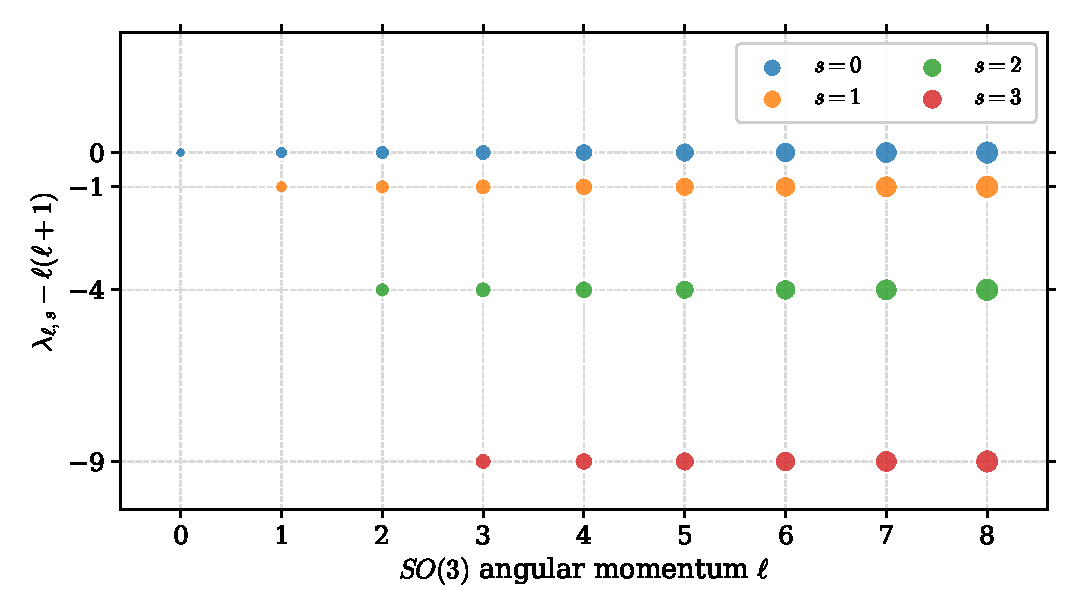
\includegraphics[width=.83\linewidth]{content/MathSkills/figures/geometry-highspin/spin_weight_bundle_spectrum.pdf}
\caption{单位二球带整数权 $s$ 的齐性线丛粗拉普拉斯谱 $\lambda_{\ell,s}=\ell(\ell+1)-s^2$。纵坐标是相对于标量 Casimir 的位移 $\lambda_{\ell,s}-\ell(\ell+1)=-s^2$，点大小与简并度 $2\ell+1$ 成正比，左端缺失的点体现最低允许 $\ell=|s|$。此图不是 Hodge 拉普拉斯算子的全部一形式谱，更不能将 $s$ 当作平直环面上的 Fourier 波矢。}\label{fig:ghs-r9-spin-weight-spectrum}
\end{figure}

\cref{fig:ghs-r9-spin-weight-spectrum} 把前文的齐性空间重数公式变成可阅读的谱图：同样是“自旋”，球面的局部纤维权 $s$ 通过稳定子表示限制允许出现的 $SO(3)$ 角动量 $\ell$；环面上的纵横分解却来自外微分代数。二者可以在同一高自旋问题中同时出现，但数学上不是同一个分解。

\section{热半群、热迹与局域几何}
在同一纤维内作酉基底变换，只会改变算子的矩阵表示，并不会改变它的谱。

\begin{proposition}[酉丛变换与谱不变性]
\label{prop:ghs-r6-gauge-unitary}
设 $U:E\to E$ 是光滑的逐点酉丛自同构，并令 $\nabla'=U\nabla^EU^{-1}$、$V'=UVU^{-1}$。在映到彼此的算子定义域上，$A'=UAU^{-1}$；因而二者的谱测度、重数及热迹（若存在）相同。

\end{proposition}
\begin{proof}
对任意截面 $u$，$\nabla'(Uu)=U\nabla^Eu$。由于 $U$ 保持纤维内积和体积测度，取形式伴随后有 $\nabla'{}^*(U\alpha)=U\nabla^{E*}\alpha$，再作用一次即得 $A'(Uu)=UAu$。若边界条件也由 $U$ 传送，$U$ 将闭算子的定义域双射到新定义域，故 $A'$ 与 $A$ 酉等价。对 Borel 函数 $f$，谱演算还给出 $f(A')=Uf(A)U^{-1}$，结论成立。
\end{proof}

设 $A$ 是下有界自伴实现，先减去一个常数使 $A\ge0$。谱定理给出投影值测度 $\mathsf E_A$，以及
\begin{equation}\label{eq:ghs-r6-heat-functional-calculus}
T(t)=\ee^{-tA}=\int_{[0,\infty)}\ee^{-t\lambda}\,\dd\mathsf E_A(\lambda),\qquad t\ge0.
\end{equation}
这里 $t$ 的量纲是长度平方；它是热演化参数，不是物理时间。由谱积分相乘可知 $T(t+s)=T(t)T(s)$、$\norm{T(t)}\le1$，并且 $T(t)$ 在 $t\downarrow0$ 时强收敛到恒等算子。若 $A$ 的谱离散且本征截面 $u_j$ 构成完备正交基，
\[
T(t)f=\sum_j\ee^{-t\lambda_j}\langle f, u_j\rangle u_j,
\qquad H_t(x,y)=\sum_j\ee^{-t\lambda_j}u_j(x)u_j(y)^*.
\]
第二式中的 $H_t(x,y)$ 是从 $E_y$ 到 $E_x$ 的线性映射；不能把向量丛值热核误写成没有平行移动意义的标量函数。

\begin{figure}[htbp]
\centering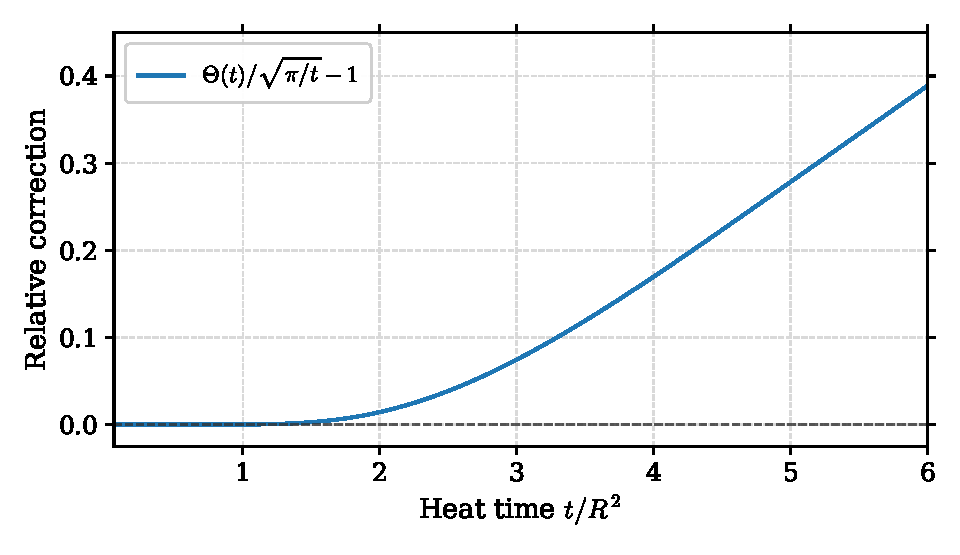
\includegraphics[width=.79\linewidth]{content/MathSkills/figures/geometry-highspin/heat_trace_circle.pdf}
\caption{单位半径圆周上的精确热迹 $\Theta(t)=\sum_{n\in\mathbb Z}\ee^{-n^2t}$ 与 Weyl 主项 $\sqrt{\pi/t}$ 的相对偏差。零参考线表示局部 Weyl 预测；短热时间的领先偏差由 Poisson 求和中的 $2\ee^{-\pi^2/t}$ 控制。}\label{fig:ghs-heat-trace-circle}
\end{figure}

\cref{fig:ghs-heat-trace-circle} 使热核与全局拓扑之间的关系可见：$t\downarrow0$ 时先读到局部体积，闭合路径的影响则以 $\ee^{-\pi^2/t}$ 的非幂级数方式出现。

\begin{theorem}[热核拼接与正算子性质]\label{thm:ghs-r6-heat-gluing}
若 $A$ 在紧致无边界流形上是非负自伴拉普拉斯型算子，则 $t>0$ 时热核光滑，并满足
\begin{equation}\label{eq:ghs-r6-heat-convolution}
H_{t+s}(x,y)=\int_MH_t(x,z)H_s(z,y)\dd\mu_g(z),
\qquad H_t(x,y)^*=H_t(y,x).
\end{equation}
当纤维秩为 $1$ 且 $A=-\Delta+V$、$V$ 为实函数时，正性保持的半群还满足正数据不会产生负值的性质；对任意向量丛上的矩阵势不能仅从 $A\ge0$ 推出逐分量非负。
\end{theorem}
\begin{proof}
谱演算给 $T(t+s)=T(t)T(s)$。将两个积分核逐次作用于测试截面并运用 Fubini 定理，就得到第一式；对有限谱截断可逐项验证，再使用光滑性和适当核收敛完成极限。自伴性给 $T(t)^*=T(t)$，故得到第二式。标量正性保持可由热方程的最大值原理证明；丛值截面没有自然的逐点全序，最后的区别来自这一基本事实。
\end{proof}

高能谱为什么只在领先阶感受到体积，而较低阶逐渐感受到曲率？在短热时间中，热量只能沿很短的测地线传播，因此热核接近欧氏空间上的 高斯 核。取正算子 $A=\nabla^{E*}\nabla^E+V$，在紧致无边界光滑流形上有渐近式
\begin{equation}\label{eq:ghs-r6-heat-local-coefficients}
\operatorname{Tr}_{E_x}H_t(x,x)\sim\frac1{(4\pi t)^{n/2}}
\operatorname{tr}_E\left[\id+t\left(\frac{\mathcal R}{6}\id-V\right)+O(t^2)\right].
\end{equation}
此处 $\mathcal R$ 是标量曲率。$O(t^2)$ 应按局部光滑渐近展开理解，不保证该级数对固定 $t$ 收敛。若使用 $A=-(g^{ab}\nabla_a\nabla_b+\mathcal E)$ 的常见另一种约定，$V=-\mathcal E$，所以一次系数应写 $\mathcal E+\mathcal R/6$；符号不能在两个约定之间随意搬用。

我们先解释可直接计算的 $V$ 项。设平直空间上 $V=v$ 是常数，则 Fourier 变换把 $A=-\Delta+v$ 化为乘法 $|k|^2+v$，从而
\[
H_t(x,x)=\int_{\RR^n}\frac{\dd^nk}{(2\pi)^n}\ee^{-t(|k|^2+v)}
=(4\pi t)^{-n/2}\ee^{-tv}
=(4\pi t)^{-n/2}(1-tv+O(t^2)).
\]
这一步固定了势项的负号。曲率项 $\mathcal R/6$ 则来自法坐标中 高斯 传播与体积 雅可比因子 的二阶修正；一般情形需要将测地世界函数、Van Vleck 行列式和热方程递推一起处理，不能仅对体积因子做 Taylor 展开便声称证明了完整系数。相应的标准局部热核构造可参照 \cite{r6-vassilevich,r6-gilkey} 中的参数核方法。

在两个点由唯一短测地线连接的凸正规邻域内，定义半测地距离平方
$\Sigma(x,y)=\tfrac12\operatorname{dist}_g(x,y)^2$，令 $D_a$ 表示 $E$ 上的联络。它满足 eikonal 恒等式
\[
 g^{ab}(D_a\Sigma)(D_b\Sigma)=2\Sigma.
\]
为使局部核的最高短时间行为与欧氏 高斯 相同，设
\begin{equation}\label{eq:ghs-r6-parametrix-ansatz}
H_t(x,y)\sim (4\pi t)^{-n/2}\ee^{-\Sigma(x,y)/(2t)}
\sum_{j\ge0}t^ja_j(x,y),
\end{equation}
其中 $a_j(x,y):E_y\to E_x$，对一般向量丛不能把它们当作无指标的数。先求指数的一阶、二阶协变导数：
\begin{align*}
D_a\ee^{-\Sigma/(2t)}
&=-\frac{D_a\Sigma}{2t}\ee^{-\Sigma/(2t)},\\
D^aD_a\ee^{-\Sigma/(2t)}
&=\left[\frac{|D\Sigma|^2}{4t^2}
 -\frac{\Delta\Sigma}{2t}\right]\ee^{-\Sigma/(2t)}.
\end{align*}
对任意丛值振幅 $a$ 使用乘积法则，则
\[
D^aD_a(\ee^{-\Sigma/(2t)}a)
=\ee^{-\Sigma/(2t)}\left[D^aD_aa
 -\frac{D^a\Sigma}{t}D_aa
 +\left(\frac{2\Sigma}{4t^2}-\frac{\Delta\Sigma}{2t}\right)a\right].
\]
把 \cref{eq:ghs-r6-parametrix-ansatz} 代入热方程 $(\partial_t+A_x)H_t=0$，其中 $A=-D^aD_a+V$。$t^{-2}$ 项来自指数的时间导数和空间 拉普拉斯算子；由于 eikonal 恒等式，它们恰好抵消。$t^{-1}$ 阶得到领先运输方程
\begin{equation}\label{eq:ghs-r6-heat-a0-transport}
\left[2D^a\Sigma D_a+\Delta\Sigma-n\right]a_0=0,
\qquad a_0(y,y)=\id.
\end{equation}
匹配其后 $t^{j-1}$ 系数，得到递推式
\begin{equation}\label{eq:ghs-r6-heat-aj-transport}
\left[2D^a\Sigma D_a+\Delta\Sigma-n+2j\right]a_j
=2(D^aD_a-V)a_{j-1},\qquad j\ge1.
\end{equation}
这一关系是局部渐近构造的真正动力：每一级系数都由前一级沿测地线的输运决定，而不是逐阶猜测曲率不变量。

当 $x\to y$ 时有 $D\Sigma=0$、$\Delta\Sigma=n$，所以对于 $j=1$，
$a_1(y,y)=(D^aD_aa_0)(y,y)-V(y)$。在 $y$ 的测地法坐标与平行纤维框架中，\cref{eq:ghs-r6-heat-a0-transport} 的解为
\[
a_0(x,y)=\Delta_{\rm VM}(x,y)^{1/2}\mathcal P_{y\to x},
\]
其中 $\mathcal P_{y\to x}$ 是联络平行移动，$\Delta_{\rm VM}$ 是 Van Vleck 行列式。

用 Jacobi 场与正规坐标的体积膨胀可得到
\[
\Delta_{\rm VM}(x,y)^{1/2}
=1+\frac1{12}\operatorname{Ric}_{ab}(y)x^ax^b+O(|x|^3).
\]
平行框架中平行移动对角点的 拉普拉斯算子 收缩没有附加一阶曲率项，因为联络曲率在导数指标上反对称。于是
\[
(D^aD_aa_0)(y,y)=\frac16\mathcal R(y)\id,
\quad a_1(y,y)=\frac16\mathcal R(y)\id-V(y),
\]
恰好恢复 \cref{eq:ghs-r6-heat-local-coefficients}。

这证明了局部一次热核系数；关于余项在一般几何上的一致控制仍需参数核误差估计。

\begin{proposition}[热迹控制 Weyl 系数]\label{prop:ghs-r6-tauberian-weyl}
若 $A$ 在秩 $r$ 的丛上为非负椭圆拉普拉斯型算子，$M$ 紧致无边界，则
\begin{equation}\label{eq:ghs-r6-leading-weyl}
N_A(\Lambda)\sim\frac{r\,\omega_n\operatorname{Vol}(M)}{(2\pi)^n}\Lambda^{n/2}
\qquad(\Lambda\to\infty).
\end{equation}
\end{proposition}
\begin{proof}
对谱计数测度 $\dd N_A$，热迹恰为其 Laplace 变换：
\[
\operatorname{Tr}(\ee^{-tA})=\sum_j\ee^{-t\lambda_j}
=\int_{[0,\infty)}\ee^{-t\lambda}\,\dd N_A(\lambda).
\]
将 \cref{eq:ghs-r6-heat-local-coefficients} 的主项沿 $M$ 积分得
$\operatorname{Tr}(\ee^{-tA})\sim r\operatorname{Vol}(M)(4\pi t)^{-n/2}$。
非减函数的 Tauber 定理把这一热迹渐近变为
$N_A(\Lambda)\sim r\operatorname{Vol}(M)\Lambda^{n/2}/[(4\pi)^{n/2}\Gamma(1+n/2)]$。
由于 $\omega_n=\pi^{n/2}/\Gamma(1+n/2)$，即为所列公式。最后一步调用 Tauber 定理而非简单逐项逆 Laplace 变换；原因是点态谱计数含阶梯函数。
\end{proof}

\subsection{二球热核与角动量截断}
\label{sec:ghs-heat-kernel-boundary}

若 $A\ge m^2>0$，对每个谱值都有 $\lambda^{-1}=\int_0^\infty\ee^{-t\lambda}\dd t$，从而
\begin{equation}\label{eq:ghs-r6-green-propertime}
A^{-1}=\int_0^\infty\ee^{-tA}\dd t.
\end{equation}
这里积分在算子范数中收敛，其范数由 $m^{-2}$ 控制。若 $A\ge0$ 但有非平凡零模，原积分沿零模发散；在紧致情形应先定义正交投影 $\Pi_0$，改用
\[
A^+=\int_0^\infty\bigl(\ee^{-tA}-\Pi_0\bigr)\dd t.
\]
该式还需正谱离零有间隙；对连续谱逼近零点的非紧空间，一般只能在指定的加权空间、二次型或分布意义下解释。这是算子定义域与红外行为不能分开的一个例子。

例如，在圆周与球面的热迹的计算中，
\label{ex:ghs-r6-circle-heat}
长度为 $L$ 的平直圆周有 $\lambda_k=(2\pi k/L)^2$。Poisson 求和给出
\[
\sum_{k\in\ZZ}\ee^{-4\pi^2tk^2/L^2}
=\frac{L}{\sqrt{4\pi t}}\sum_{m\in\ZZ}\ee^{-m^2L^2/(4t)}.
\]
因此 $t\downarrow0$ 时主项是 $L/\sqrt{4\pi t}$，其余修正指数小；一维圆周的局部曲率为零。标准单位二球则有 $\lambda_\ell=\ell(\ell+1)$、重数 $2\ell+1$，热迹领先项 $\operatorname{Area}(S^2)/(4\pi t)=t^{-1}$，并有来自 $\mathcal R/6=1/3$ 的常数项。两个例子说明曲率、拓扑与空间维数以不同阶次进入谱。

\begin{figure}[htbp]
\centering
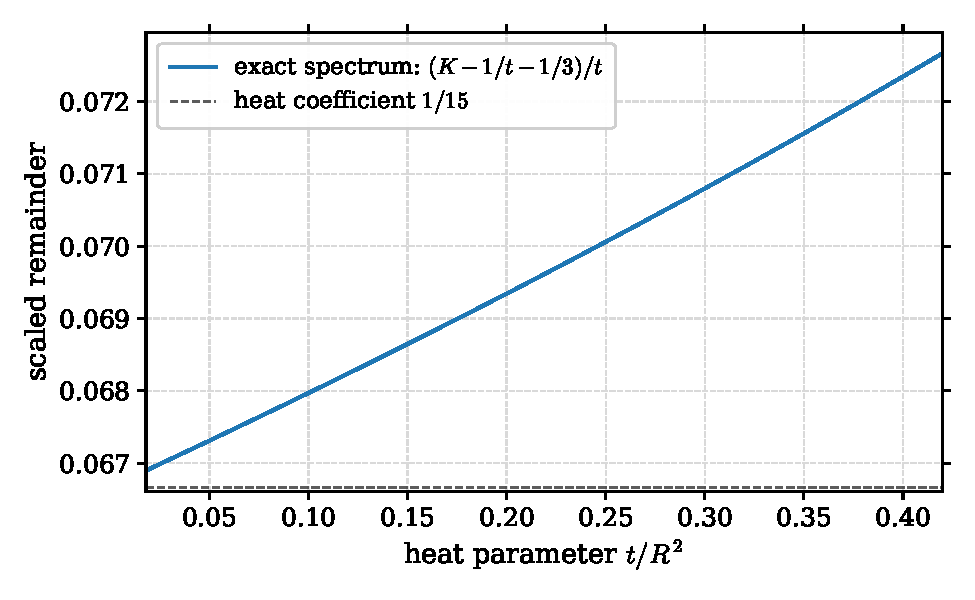
\includegraphics[width=.78\linewidth]{content/MathSkills/figures/geometry-highspin/heat_curvature_remainder.pdf}
\caption{单位二球热迹去掉 Weyl 主项 $t^{-1}$ 和曲率常数项 $1/3$ 后的缩放余项。精确谱求和趋向下一阶系数 $1/15$，显示不同几何数据进入不同的热时间阶数。}
\label{fig:ghs-r6-heat-remainder}
\end{figure}

一般向量丛热核的参数核需要联络与曲率输运，初次接触时很容易变成一串抽象系数。单位二球是一个有用的完整算例：它不仅有离散谱，而且存在可以直接把全部模态求和为一个按测地距离变化的核的加法定理。借此既能看见扩散的空间形状，也能检验短时间曲率系数与截断误差。

令 $\Sigma=S_R^2$ 为半径 $R$ 的标准球面，令 $A=-\Delta_{S_R^2}$ 作用于标量，热参数 $t>0$ 的单位为长度平方。球谐满足
\[
 AY_{\ell m}=\frac{\ell(\ell+1)}{R^2}Y_{\ell m},\qquad
 \sum_{m=-\ell}^{\ell}|Y_{\ell m}(x)|^2=\frac{2\ell+1}{4\pi R^2}.
\]
这里球谐按 $\int_{S_R^2}|Y_{\ell m}|^2\dd\mu=1$ 归一化，因而与单位球面常用的球谐相差一个 $R^{-1}$。

对两个点 $x,y$，定义 $\theta=d(x,y)/R\in[0,\pi]$。旋转不变性说明 $\sum_mY_{\ell m}(x)\overline{Y_{\ell m}(y)}$ 只能依赖 $\theta$；在北极 $x$ 固定后解 Legendre 方程，并取 $\theta=0$ 归一，即得到加法定理
\[
 \sum_{m=-\ell}^{\ell}Y_{\ell m}(x)\overline{Y_{\ell m}(y)}
 =\frac{2\ell+1}{4\pi R^2}P_\ell(\cos\theta).
\]

\begin{theorem}[二球热核的精确谱展开]
\label{thm:ghs-r9-sphere-heat}
在无边界的标准二球上，热核 $K_t(x,y)$ 是下列绝对且对 $t\ge t_0>0$ 一致收敛的级数：
\begin{equation}\label{eq:ghs-r9-sphere-heat}
 K_t(\theta)=\frac1{4\pi R^2}\sum_{\ell=0}^{\infty}
 (2\ell+1)\ee^{-t\ell(\ell+1)/R^2}P_\ell(\cos\theta).
\end{equation}
它满足 $\partial_tK_t=\Delta_xK_t$、$K_t(x,y)=K_t(y,x)$、$K_t>0$（$t>0$）及
\begin{equation}\label{eq:ghs-r9-sphere-heat-mass}
 \int_{S_R^2}K_t(x,y)\dd\mu_y=1,
 \qquad \lim_{t\to\infty}K_t(x,y)=\frac1{4\pi R^2}.
\end{equation}
\end{theorem}
\begin{proof}
将 $A$ 的谱定理与加法定理代入 $\ee^{-tA}$ 的积分核便得到 \cref{eq:ghs-r9-sphere-heat}。因为 $|P_\ell(z)|\le1$ 对 $z\in[-1,1]$ 成立，而 $(2\ell+1)\ee^{-t_0\ell(\ell+1)/R^2}$ 可求和，故对 $t\ge t_0$ 一致收敛；逐项微分所需的多项式因子也被指数衰减压住。$\partial_tK_t=\Delta_xK_t$ 由每个本征模态的热方程得出。

质量守恒可直接沿 $y$ 积分：对 $\ell\ge1$，Legendre 正交性给 $\int_{-1}^1P_\ell(z)\dd z=0$，唯有 $\ell=0$ 的积分留下 $1$。长时间极限同样只剩 $\ell=0$。严格的 $K_t>0$ 由连通紧致流形上热方程的强最大值原理得到，而不应仅凭交替符号的 Legendre 级数逐项猜测。
\end{proof}

\begin{figure}[htbp]
\centering% Great-circle cross-section of an S2; geodesic arc vs embedding chord.
\begin{tikzfig}[scale=1.0]
\coordinate (O) at (0,0);
\coordinate (P) at (0,2.15);
\coordinate (Q) at (1.97,.86);
\draw[thick] (O) circle (2.15);
\fill (O) circle (1.7pt);
\fill (P) circle (2.6pt);
\fill (Q) circle (2.6pt);
\draw[gray,dashed] (O)--(P) (O)--(Q);
\draw[gray!70,dashed] (P)--(Q);
\draw[line width=1.6pt] (P) arc[start angle=90,end angle=23.6,radius=2.15];
\draw[lecturearrow] (.0,.74) arc[start angle=90,end angle=23.6,radius=.74];
\node[lecturelabel] at (.50,.94) {$\theta$};
\node[lecturelabel] at (.33,2.54) {Source $x$};
\node[lecturelabel] at (2.58,.85) {Target $y$};
\node[lecturelabel] at (2.9,2.07) {$s=R\theta$};
\node[lecturelabel] at (3.45,-.17) {Chord $2R\sin(\theta/2)$};
\draw[lecturearrow] (1.91,-.05)--(1.20,.70);
\node[lecturelabel] at (-.34,-.34) {$O$};
\node[lecturelabel] at (-1.60,-1.67) {$S_R^2$ section};
\end{tikzfig}

\caption{从球面一点发出的热传播按测地角 $\theta=d(x,y)/R$ 组织，而不是按欧氏弦长 $|x-y|$。球面的闭合性使扩散最终收敛到均匀密度 $1/(4\pi R^2)$；短时间则主要由局部的短测地线控制。}\label{fig:ghs-r9-sphere-heat-geodesic}
\end{figure}
\begin{figure}[htbp]
\centering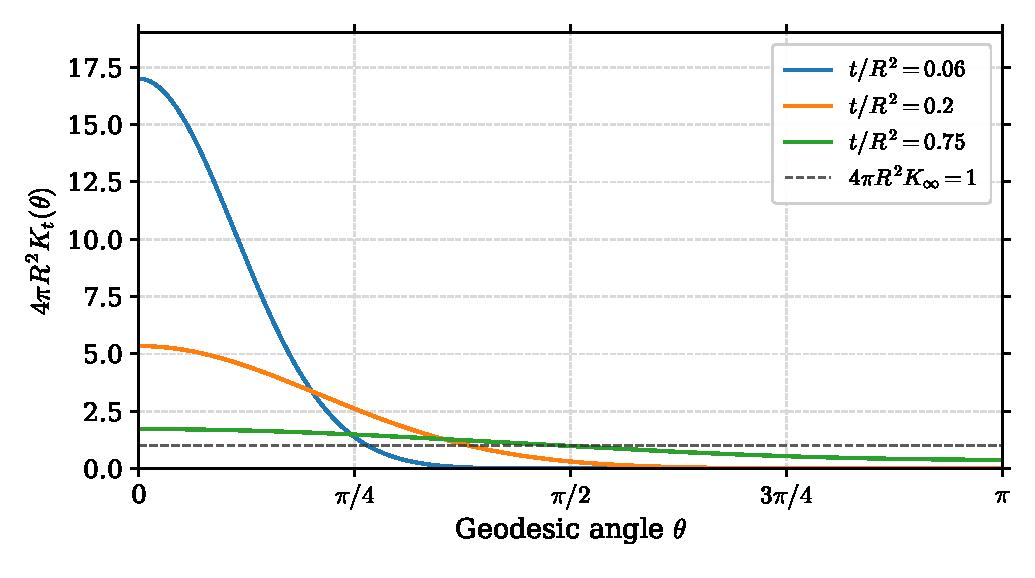
\includegraphics[width=.83\linewidth]{content/MathSkills/figures/geometry-highspin/sphere_heat_geodesic_profiles.pdf}
\caption{半径 $R=1$ 的二球热核，纵轴为 $4\pi R^2K_t(\theta)$，横轴为测地角 $\theta$。曲线由 \cref{eq:ghs-r9-sphere-heat} 的 Legendre 级数直接计算；虚线 $1$ 是保留总概率的长时间均匀极限。越短的热时间越接近局部 高斯，越长的热时间越显现紧致性。}\label{fig:ghs-r9-sphere-heat-profiles}
\end{figure}

短时间的对角热核可以从本章的一般曲率系数独立检查。二球标量曲率为 $\mathcal R=2/R^2$，故
\begin{equation}\label{eq:ghs-r9-sphere-heat-diagonal}
 K_t(0)=\frac1{4\pi t}\left[1+\frac{t}{3R^2}+O\!\left(\frac{t^2}{R^4}\right)\right],
 \qquad t\downarrow0.
\end{equation}
为了不把 $t^{-1}$ 的发散遮住真正的曲率信号，定义无量纲诊断量
\[
 C(q)=\frac{4\pi tK_t(0)-1}{q},\qquad q=t/R^2.
\]
由 \cref{eq:ghs-r9-sphere-heat-diagonal}，$C(q)\to1/3$。继续使用 Euler--Maclaurin 公式对 $F(x)=(2x+1)\ee^{-qx(x+1)}$ 求和，积分项严格为 $\int_0^\infty F(x)\dd x=1/q$，端点修正给出
\begin{equation}\label{eq:ghs-r9-sphere-heat-asymptotic}
 \sum_{\ell\ge0}(2\ell+1)\ee^{-q\ell(\ell+1)}
 =\frac1q+\frac13+\frac q{15}+O(q^2),
 \qquad q\downarrow0.
\end{equation}
于是更精细的残差 $(C(q)-1/3)/q\to1/15$。这一诊断量在有限数值精度下比原始热核更灵敏地暴露曲率项和截断错误。

\begin{figure}[htbp]
\centering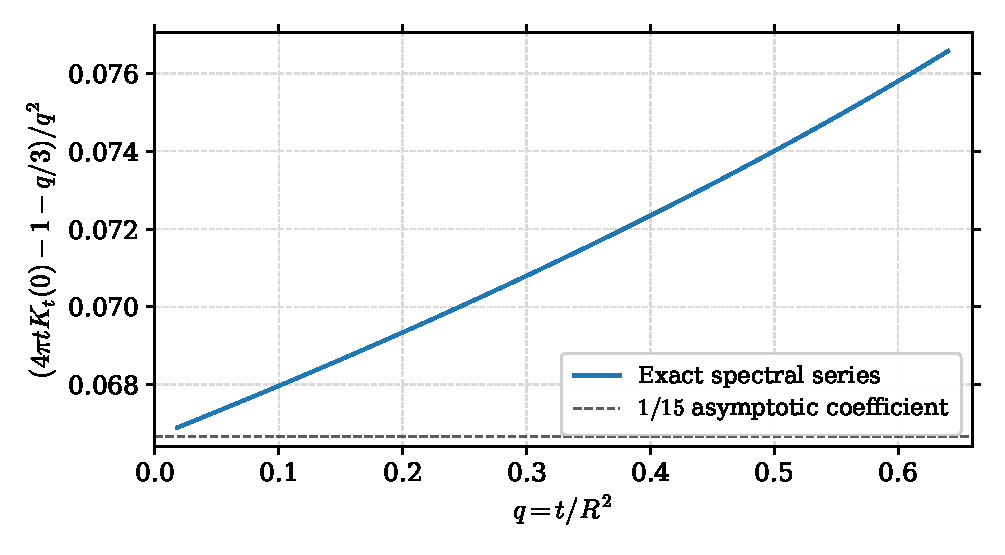
\includegraphics[width=.79\linewidth]{content/MathSkills/figures/geometry-highspin/sphere_heat_curvature_residual.pdf}
\caption{二球对角热核的谱级数数值验证：$[4\pi tK_t(0)-1-q/3]/q^2$ 在 $q=t/R^2\to0$ 时趋于 $1/15$。图采用足够的角动量截断，避免把有限截断的缺失高频模态误读成热核的几何系数。}\label{fig:ghs-r9-sphere-heat-residual}
\end{figure}

\begin{proposition}[热核角动量截断的显式误差]
\label{prop:ghs-r9-sphere-heat-tail}
令 $K_t^{(L_0)}$ 为 \cref{eq:ghs-r9-sphere-heat} 截到 $\ell=L_0$ 的部分和，令 $q=t/R^2$。若 $L_0+1\ge (\sqrt{2/q}-1)/2$，则任意 $\theta\in[0,\pi]$ 都有
\begin{equation}\label{eq:ghs-r9-sphere-heat-tail-bound}
 |K_t(\theta)-K_t^{(L_0)}(\theta)|
 \le \frac{\ee^{-q(L_0+1)(L_0+2)}}{4\pi R^2}
 \left(2L_0+3+\frac1q\right).
\end{equation}
\end{proposition}
\begin{proof}
由 $|P_\ell|\le1$，误差至多为 $\sum_{\ell=L_0+1}^\infty f(\ell)/(4\pi R^2)$，其中 $f(x)=(2x+1)\ee^{-qx(x+1)}$。条件保证 $f'(x)\le0$ 对 $x\ge L_0+1$ 成立，于是积分比较给出
\[
 \sum_{\ell=L_0+1}^{\infty}f(\ell)
 \le f(L_0+1)+\int_{L_0+1}^{\infty}f(x)\dd x.
\]
因为 $\frac{\dd}{\dd x}\ee^{-qx(x+1)}=-qf(x)$，积分恰等于 $q^{-1}\ee^{-q(L_0+1)(L_0+2)}$，代回即得。
\end{proof}

这个误差界给绘图提供了可检查的截断条件，并解释为什么热时间越短，必须保留的高角动量就越多。它仅保证经典球面标量热核的这一谱截断；在一般流形或张量丛上，应以本征值增长及谱投影估计重新建立相应尾界，不能直接沿用 Legendre 多项式的界。

\section{高频计数与半经典传播}
\begin{equation}\label{eq:ghs-weyl-law-sigma}
 N_A(\Lambda)=\frac{\operatorname{Vol}(\Sigma)\,\omega_{d-1}}{(2\pi)^{d-1}}
 \Lambda^{(d-1)/2}+o\bigl(\Lambda^{(d-1)/2}\bigr).
\end{equation}
这里真正普遍的是高能态密度对体积与维数的依赖，而不是球谐的 $\ell(\ell+d-2)$ 本征值。球对称是谱可显式求和的特殊幸运情形。

\begin{figure}[htbp]
\centering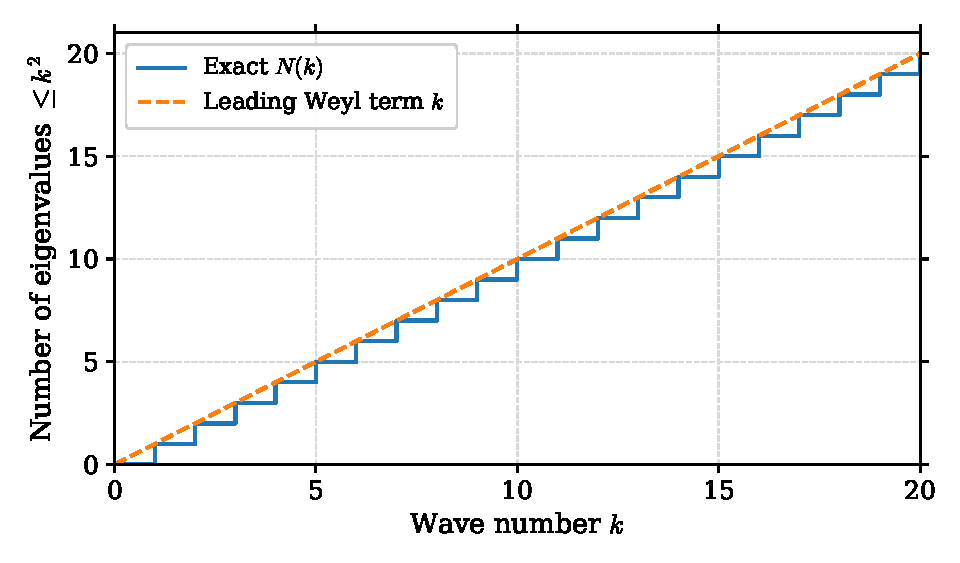
\includegraphics[width=.79\linewidth]{content/MathSkills/figures/geometry-highspin/weyl_staircase.pdf}
\caption{区间 $(0,\pi)$ 上 Dirichlet 算子 $-\partial_x^2$ 的精确阶梯谱计数 $N(k^2)=\lfloor k\rfloor$ 与 Weyl 主项 $k$。竖直跳跃来自离散本征值；主项不解析这些振荡。}\label{fig:ghs-weyl-staircase}
\end{figure}

\cref{fig:ghs-weyl-staircase} 是 Weyl 律的最简单可直接核算的模型，也提醒我们渐近公式给出的是大尺度增长，不会逐个预测本征值。

对高频态的计数，也可以直接按经典相空间体积计算。
在小坐标块中冻结系数，把特征函数近似看成局域平面波。每个相空间量子态占据 $(2\pi)^{d-1}$ 的无量纲相空间体积。满足主符号 $h^{ab}p_ap_b\leq\Lambda$ 的协变量在每点形成椭球；其体积是 $\omega_{d-1}\Lambda^{(d-1)/2}\sqrt{\det h}$。对 $\Sigma$ 积分并除以 $(2\pi)^{d-1}$，得到 \cref{eq:ghs-weyl-law-sigma} 的主项。严格证明还需微局部分析控制坐标块边界与高频误差；这里的相空间计算只用于解释严格 Weyl 定理的系数，不取代其误差证明。

自伴性确定谱演算的数学合法性，而空间对称性决定谱的简并规律。两者不同：即使曲率破坏全部连续等距对称，谱定理仍成立；只是再没有普遍意义上的角动量量子数可用。

高自旋与高频不是同一个概念：前者是群表示标签，后者来自微分算子的谱。如果空间不是球面，未必存在自旋 $S$ 的全局角模态，但仍可以考察 $-\Delta$ 的高本征值极限。半经典分析提供一套几乎不依赖特殊坐标的近似，它将高频传播的主导轨迹联系到测地流，并明确误差何时失去控制。

设 $A_h=-h^2\Delta_g+V$，这里 $h>0$ 是无量纲小参数，与截面度规 $h_{ab}$ 的符号无关。它的经典主符号为
\begin{equation}\label{eq:ghs-semiclassical-principal-symbol}
 p(x,\xi)=g^{ab}(x)\xi_a\xi_b+V(x).
\end{equation}
在余切丛 $T^*M$ 上取典范辛形式 $\dd\xi_a\wedge\dd x^a$，Hamilton 方程为
\[
 \dot x^a=\frac{\partial p}{\partial\xi_a}=2g^{ab}\xi_b,
 \qquad\dot\xi_a=-\frac{\partial p}{\partial x^a}.
\]
当 $V$ 为常数时，轨迹投影到 $M$ 上是重新参数化的测地线。这一结论只用到了局部度规与主符号；不需要旋转群。

考虑定态方程 $A_h\psi=E\psi$，尝试振幅—相位形式 $\psi=a(x)\ee^{\ii S(x)/h}$。对其梯度与 拉普拉斯算子逐步求导，得到
\[
 \nabla_a\psi=\ee^{\ii S/h}
 \left(\nabla_aa+\frac{\ii}{h}a\nabla_aS\right),
\]
\[
 \Delta_g\psi=\ee^{\ii S/h}
 \left[\Delta_ga+\frac{2\ii}{h}\nabla^aS\nabla_aa
 +\frac{\ii}{h}a\Delta_gS-\frac1{h^2}a|\nabla S|_g^2\right].
\]
故原微分方程精确转写为
\begin{equation}\label{eq:ghs-wkb-exact-expansion}
 0=(|\nabla S|_g^2+V-E)a
 -\ii h\left(2\nabla S\cdot\nabla a+a\Delta_gS\right)
 -h^2\Delta_ga.
\end{equation}

第一项给 Hamilton--Jacobi 方程 $|\nabla S|_g^2+V=E$。第二项给振幅输运方程
\[
 2\nabla S\cdot\nabla a+a\Delta_gS=0,
 \qquad\nabla_a\bigl(a^2\nabla^aS\bigr)=0
\]
（当振幅取实时）。第三项 $-h^2\Delta_ga$ 是被舍弃的明确余项；只有当它相对于保留项受控时，近似才有意义。焦散点附近振幅可能发散、相位不再单值，需要新的局部一致近似，而不能继续用同一张 WKB 图遮盖问题。

在紧致无边界截面上，高本征值计数可视为经典能量子集
$\{(x,\xi)\in T^*\Sigma:g^{ab}\xi_a\xi_b\leq\Lambda\}$ 的相空间体积除以 $(2\pi)^{d-1}$，给出 \cref{eq:ghs-weyl-law-sigma} 的领先项。若用 $h\to0$ 参数化，则状态数按 $h^{-(d-1)}$ 增长；这是几何频率的渐近密度，而不是说所有高频本征态在空间上均匀分布。

在标准球面上，最高权谐波因旋转群表示而沿某些大圆附近集中；在其他流形上，局部高频 WKB 可以沿测地轨迹形成集中，但同时可能存在模态疤痕、退化、隧穿或量子遍历性等不同现象。高频谱的总体 Weyl 律并不能单独决定单个本征函数的分布。

因此球面对称自由场模型中“高 $S$ 产生对径峰”的精确公式应始终与其自由、球面对称、特定初级态及场振幅测量的假设绑定。一般空间的正确替代语言是：先指定算子与谱投影，再考察高频、半经典测地流和所选态核的局部集中；未出现角动量表示时，不能强加 $S\to\infty$ 的球面式几何结论。

\section{共形变换与翘曲积的径向约化}




有了任意流形上的微分算子，才可以精确回答“径向量子化为什么偶尔变得特别简单”：当空间的尺度变化可以变成柱面时间平移，而且场方程在 Weyl 变换下具有受控的协变性时，一般随时间变化的背景才简化为静态谱问题。这个性质依赖度规的具体几何，不能单靠把一个坐标命名为 $r$ 得到。

\subsection{共形拉普拉斯}
\label{sec:ghs-conformal-laplacian}

对 $d>2$，定义 $\delta=(d-2)/2$ 和 $\xi_d=(d-2)/[4(d-1)]$。共形 拉普拉斯算子（Yamabe 算子）为
\begin{equation}\label{eq:ghs-yamabe-definition}
 L_g=-\Delta_g+\xi_d\mathcal R_g.
\end{equation}
其特殊系数可以直接由 Weyl 变换决定，而不是事先猜测。

\begin{theorem}[共形 拉普拉斯算子的协变性]
\label{thm:ghs-yamabe-covariance}
若 $\widehat g=\ee^{2\sigma}g$，则任意光滑标量 $f$ 满足
\begin{equation}\label{eq:ghs-yamabe-weyl-covariance}
 L_{\widehat g}\bigl(\ee^{-\delta\sigma}f\bigr)
 =\ee^{-(\delta+2)\sigma}L_g f.
\end{equation}
\end{theorem}
\begin{proof}
由度规和行列式变换直接计算，$\widehat g^{ab}=\ee^{-2\sigma}g^{ab}$ 与 $\sqrt{\widehat g}=\ee^{d\sigma}\sqrt g$ 给出
\[
 \Delta_{\widehat g}u=\ee^{-2\sigma}
 \bigl(\Delta_g u+(d-2)\nabla\sigma\cdot\nabla u\bigr).
\]
另一方面，Levi--Civita 联络差为
\[
 \widehat\Gamma^a{}_{bc}-\Gamma^a{}_{bc}
 =\delta^a_b\partial_c\sigma+\delta^a_c\partial_b\sigma-g_{bc}\nabla^a\sigma.
\]
把这个差代入 Ricci 曲率定义并缩并，得到
\[
 \mathcal R_{\widehat g}=\ee^{-2\sigma}
 \left[\mathcal R_g-2(d-1)\Delta_g\sigma-(d-1)(d-2)|\nabla\sigma|^2\right].
\]
对 $u=\ee^{-\delta\sigma}f$ 使用乘法求导：
\begin{align*}
\Delta_gu=\ee^{-\delta\sigma}\bigl[\Delta_gf
 -2\delta\nabla\sigma\cdot\nabla f
 -\delta(\Delta\sigma)f+\delta^2|\nabla\sigma|^2f\bigr].
\end{align*}
于是 $\Delta_{\widehat g}u$ 中一阶导数系数为 $-2\delta+d-2=0$；曲率项与 $\Delta\sigma$ 的系数合并为 $\delta-2\xi_d(d-1)=0$；与 $|\nabla\sigma|^2$ 的系数合并为 $\delta^2-\xi_d(d-1)(d-2)=0$。余下项恰为 \cref{eq:ghs-yamabe-weyl-covariance}。
\end{proof}

该定理是单个共形标量微分算子的变换律。路径积分测度的量子 Weyl 异常、边界反常项及零模结构另有内容，不能从这个经典恒等式直接推出整个量子场论在任意空间上严格 Weyl 不变。

设 $(\Sigma,h)$ 为维数 $d-1$ 的紧致黎曼流形，考虑其度规圆锥
\begin{equation}\label{eq:ghs-metric-cone}
 C(\Sigma)=\RR_{>0}\times\Sigma,
 \qquad g_C=\dd r^2+r^2h.
\end{equation}
圆锥顶点 $r=0$ 通常是奇点；只有特殊的截面几何允许平滑补上顶点。作变量代换 $u=\log(r/R)$ 后
\[
 g_C=r^2(\dd u^2+h),\qquad g_{\rm cyl}=\dd u^2+h.
\]
这在任意 $h$ 下都成立，却没有说 $C(\Sigma)$ 与 $\RR^d$ 等距。

\begin{figure}[htbp]
\centering
% Local TikZ geometry; styles inherited exclusively from the shared preamble.
\begin{tikzfig}[scale=1]
\fill[gray!10] (0,0)--(-2.25,2.45) arc[start angle=180,end angle=360,x radius=2.25,y radius=.56]--cycle;
\draw[thick] (0,0)--(-2.25,2.45) (0,0)--(2.25,2.45);
\draw[thick] (-2.25,2.45) arc[start angle=180,end angle=360,x radius=2.25,y radius=.56];
\draw[dashed,gray] (2.25,2.45) arc[start angle=0,end angle=180,x radius=2.25,y radius=.56];
\draw[gray,dashed] (-.95,1.03) arc[start angle=180,end angle=360,x radius=.95,y radius=.25];
\fill (0,0) circle (1.7pt) node[below] {$r=0$};
\draw[lecturearrow] (.05,.08)--(1.4,1.57) node[midway,right] {$r$};
\node[lecturelabel] at (0,3.27) {Section $\Sigma$};
\node[lecturelabel] at (3.65,1.4) {$g=\dd r^2+r^2\gamma$};
\end{tikzfig}

\caption{度规圆锥 $g=\dd r^2+r^2h$ 的示意：径向距离 $r$ 和截面 $\Sigma$ 是两种独立几何数据。顶点附近是否光滑取决于截面度规，不能由图形的锥面外观判断。}\label{fig:ghs-metric-cone}
\end{figure}

\cref{fig:ghs-metric-cone} 中的每一层截面在内禀度规上按 $r^2$ 缩放，这正是 \cref{eq:ghs-cone-laplace} 中角向 拉普拉斯算子 伴随 $r^{-2}$ 的原因。

\begin{proposition}[圆锥上的径向 拉普拉斯算子 与标量曲率]
\label{prop:ghs-cone-laplacian}
对 \cref{eq:ghs-metric-cone}，
\begin{align}
\Delta_{g_C}&=\partial_r^2+\frac{d-1}{r}\partial_r+\frac1{r^2}\Delta_h,
 \label{eq:ghs-cone-laplace}\\
\mathcal R_{g_C}&=\frac{\mathcal R_h-(d-1)(d-2)}{r^2}.
 \label{eq:ghs-cone-curvature}
\end{align}
\end{proposition}
\begin{proof}
第一式把 $\sqrt{g_C}=r^{d-1}\sqrt h$ 代入 Laplace–Beltrami 定义即可。第二式可由径向正交标架 $e_r=\partial_r$、$e_a=r^{-1}\widetilde e_a$ 的联络计算得到：截面切平面曲率为 $r^{-2}(R_h-(h\mathbin{\wedge}h))$，包含径向的截面曲率为零；缩并截面标架产生 $-(d-1)(d-2)/r^2$ 的项。球面 $\mathcal R_h=(d-1)(d-2)$ 时恰恢复平直圆锥 $\mathcal R_{g_C}=0$。
\end{proof}

令 $\varphi=r^{-\delta}\Phi$，利用 \cref{eq:ghs-yamabe-weyl-covariance} 和乘积曲率 $\mathcal R_{g_{\rm cyl}}=\mathcal R_h$，得到
\begin{equation}\label{eq:ghs-cone-yamabe-cylinder}
 L_{g_C}\varphi=r^{-\delta-2}
 \left(-\partial_u^2-\Delta_h+\xi_d\mathcal R_h\right)\Phi.
\end{equation}
若 $\mathcal R_h$ 不是常数，不能再把曲率项当作一个数字质量。定义
\begin{equation}\label{eq:ghs-cross-section-conformal-A}
 A_h=-\Delta_h+\xi_d\mathcal R_h.
\end{equation}
$A_h$ 的本征值才是圆柱振子频率平方；即使 $-\Delta_h$ 非负，$A_h$ 也可能具有负本征值。

例如，在常负曲率截面的不稳定零模的计算中，
若 $\Sigma$ 为紧致、常标量曲率 $\mathcal R_h<0$ 的流形，则常数函数是 $-\Delta_h$ 的零模，对 $A_h$ 却有本征值 $\xi_d\mathcal R_h<0$（$d>2$）。因此 $\sqrt{A_h}$ 不能定义成全部实正振子频率。此例说明几何共形等价不保证反射正性或稳定的圆柱真空。

把圆锥推广为
\[
 g=\dd r^2+a(r)^2h,
 \qquad a(r)>0.
\]
定义 $\dd u=\dd r/a(r)$ 后，$g=a(r(u))^2(\dd u^2+h)$。此时无质量共形场仍通过 \cref{eq:ghs-yamabe-weyl-covariance} 化为 $\dd u^2+h$ 上的模型。若原作用量还含有质量 $m$，则在柱面中的有效质量平方变为 $m^2a(r(u))^2$，不再是恒定谱问题。

考虑更一般的局部算子 $A(u)=-\Delta_h+\xi_d\mathcal R_h+m^2a(u)^2$，其演化 Green 函数由
\begin{equation}\label{eq:ghs-variable-cylinder-propagation}
 \bigl[-\partial_u^2+A(u)\bigr]G(u,x;u',y)
 =\delta(u-u')\delta_h(x,y)
\end{equation}
及指定边界条件唯一确定（如果所选自伴实现可逆）。不能直接以常数频率的 $\ee^{-\omega|u-u'|}$ 代替一般解。只有在演化足够缓慢且与瞬时谱隙比较有小参数时，才可能使用绝热展开；若谱隙闭合，该近似通常失效。

在翘曲度规中计算联络系数后，曲率可以逐项求出。
对于 $g=\dd r^2+a^2h$，非零混合 Christoffel 系数为 $\Gamma^r_{ab}=-aa'h_{ab}$、$\Gamma^a_{rb}=(a'/a)\delta^a_b$，截面内联络与 $h$ 相同。代入 Ricci 定义得
\[
 R_{rr}=-(d-1)\frac{a''}a,\qquad
 R_{ab}=R_{ab}[h]-\bigl[aa''+(d-2)(a')^2\bigr]h_{ab}.
\]
再与 $g^{rr}=1$、$g^{ab}=a^{-2}h^{ab}$ 缩并，得到
\begin{equation}\label{eq:ghs-warped-scalar-curvature}
 \mathcal R_g=a^{-2}\mathcal R_h
 -2(d-1)\frac{a''}a-(d-1)(d-2)\left(\frac{a'}a\right)^2.
\end{equation}
取 $a(r)=r$ 恢复 \cref{eq:ghs-cone-curvature}；取 $a(r)=\sin r$、截面为圆球时恢复单位球面的常正曲率 $d(d-1)$。

径向量子化的圆柱技巧至此可以精确定位：它是特定几何下共形 拉普拉斯算子的谱化，而不是一般流形自动拥有的尺度对称性。

共形变换给出了空间算子的协变规律。可是实际求解场方程还必须在给定度规下分离径向与角向变量，这会把曲率和几何尺度带入有效一维势。

翘曲积的角向模态并不自动构成正交的“粒子位置态”，但它们确实给出拉普拉斯算子的一个酉谱分解。与其直接记忆球面上不同阶数的径向函数，不如先把任意截面的测度和微分表达式一起变换成一维问题；这样可以逐项看出截面谱、体积膨胀和背景曲率各贡献了什么。

设 $X=I\times\Sigma$，$\dim\Sigma=m\ge1$，$h$ 是 $\Sigma$ 上与 $r$ 无关的完备黎曼度规，且 $a:I\to\RR_{>0}$ 光滑。暂取无附加势的标量 拉普拉斯算子，
\begin{equation}\label{eq:ghs-r9-warp-geometry}
 g=\dd r^2+a(r)^2h,\qquad \dd\mu_g=a(r)^m\dd r\,\dd\mu_h.
\end{equation}
若 $-\Delta_hY_j=\lambda_jY_j$ 且 $\langle Y_j, Y_i\rangle=\delta_{ij}$，则直接展开散度形式得到
\begin{align*}
\Delta_g(fY_j)
 &=\frac1{a^m}\partial_r(a^m f')Y_j+\frac{f}{a^2}\Delta_hY_j\\
 &=\left[f''+m\frac{a'}a f'-\frac{\lambda_j}{a^2}f\right]Y_j.
\end{align*}
角向变量已经分离，但仍不能把括号中的微分表达式直接当作 $L^2(I,\dd r)$ 上的 哈密顿算子，因为原径向范数含有 $a^m$。

\begin{theorem}[翘曲积 拉普拉斯算子 的酉径向约化]
\label{thm:ghs-r9-warp-unitary}
设 $\Sigma$ 紧致无边界，$a>0$，选定相容的自伴边界条件。定义
\[
(U_j f)(r)=a(r)^{m/2}f(r),\quad
U_j:L^2(I,a^m\dd r)\longrightarrow L^2(I,\dd r).
\]
则在角模态 $Y_j$ 上，$-\Delta_g$ 与下述一维 Schrödinger 算子酉等价：
\begin{equation}\label{eq:ghs-r9-warp-potential}
 H_j=-\frac{\dd^2}{\dd r^2}+V_j(r),\qquad
 V_j=\frac{\lambda_j}{a^2}+\frac m2\frac{a''}{a}
       +\frac{m(m-2)}4\left(\frac{a'}a\right)^2.
\end{equation}
若原算子含一个实乘法势 $W(r)$，右端另加 $W(r)$。酉等价的结论包含算子定义域的映射，不仅是形式微分方程相同。
\end{theorem}
\begin{proof}
置 $b=m/2$、$f=a^{-b}u$，逐次微分：
\begin{align*}
 f'&=a^{-b}\left(u'-b\frac{a'}a u\right),\\
 f''&=a^{-b}\left[u''-2b\frac{a'}a u'
 +\left(b(b+1)\frac{(a')^2}{a^2}-b\frac{a''}a\right)u\right].
\end{align*}
把两式代入 $-f''-m(a'/a)f'+\lambda_j f/a^2$。$u'$ 的系数是 $2b-m=0$；$u$ 的系数为
\begin{align*}
&-b(b+1)\frac{(a')^2}{a^2}+b\frac{a''}a
 +mb\frac{(a')^2}{a^2}+\frac{\lambda_j}{a^2}\\
&\hspace{2em}=\frac{\lambda_j}{a^2}+b\frac{a''}a
 +b(b-1)\left(\frac{a'}a\right)^2,
\end{align*}
这就是 \cref{eq:ghs-r9-warp-potential}。另一方面
\[
\int_I|f(r)|^2a(r)^m\dd r=\int_I|u(r)|^2\dd r,
\]
故 $U_j$ 等距且满射。对 $C_c^\infty(I)$ 上的表达式上述计算成立；选定自伴实现后，只有将其定义域同时映为 $U_j\operatorname{Dom}(H_j^{\rm original})$，才得到严格的算子酉等价。
\end{proof}

这个定理没有使用常曲率，也没有要求 $\Sigma$ 是球面。截面的全部几何进入 $\lambda_j$，径向体积变化进入后两项；二者在同一个势函数中相加。若 $a$ 逼近零，必须像锥尖问题一样重新判断端点的极限点/极限圆类型，不能只靠势函数图决定自伴实现。

例如，在三维常曲率空间的计算中，
令 $m=2$，截面为单位二球，$\lambda_\ell=\ell(\ell+1)$。取曲率长度 $L>0$，三个常见空间分别对应
\begin{equation}\label{eq:ghs-r9-warp-models}
 a_0(r)=r,\qquad
 a_+(r)=L\sin(r/L),\qquad
 a_-(r)=L\sinh(r/L).
\end{equation}
它们的径向区间依次为 $(0,\infty)$、$(0,\pi L)$、$(0,\infty)$，依次代表 $\RR^3$、半径 $L$ 的 $S^3$ 的极坐标，以及曲率 $-1/L^2$ 的双曲空间 $\mathbb H^3_L$。由于 $m(m-2)=0$，约化势恰为
\begin{equation}\label{eq:ghs-r9-constant-curvature-potential}
\begin{aligned}
 V_{\ell,0}&=\frac{\ell(\ell+1)}{r^2},\\
 V_{\ell,+}&=\frac{\ell(\ell+1)}{L^2\sin^2(r/L)}-\frac1{L^2},\\
 V_{\ell,-}&=\frac{\ell(\ell+1)}{L^2\sinh^2(r/L)}+\frac1{L^2}.
\end{aligned}
\end{equation}
因此曲率不仅改变角向离心势，还在双曲空间产生远距离的正阈值 $1/L^2$；而紧致球面在第二极点还有一个必需的端点条件。

\begin{figure}[htbp]
\centering% A warped-product foliation. All typography/strokes from shared preamble.
\begin{tikzfig}[scale=.90]
\coordinate (O) at (0,0);
\fill[gray!8] (-2.0,1.4) -- (-2.95,3.35) -- (2.95,3.35) -- (2.0,1.4) -- cycle;
\draw[gray!65,dashed] (-2.00,1.40) arc[start angle=180,end angle=360,x radius=2.00,y radius=.45];
\draw[gray!65] (-2.00,1.40) arc[start angle=180,end angle=0,x radius=2.00,y radius=.45];
\draw[gray!65,dashed] (-2.95,3.35) arc[start angle=180,end angle=360,x radius=2.95,y radius=.57];
\draw[gray!65] (-2.95,3.35) arc[start angle=180,end angle=0,x radius=2.95,y radius=.57];
\draw[thick] (-2,1.4)--(-2.95,3.35) (2,1.4)--(2.95,3.35);
\draw[lecturearrow] (0,-.15)--(0,4.10) node[above] {Radial distance $r$};
\draw[lecturearrow] (.10,1.38)--(1.88,1.38) node[midway,below] {$a(r_1)$};
\draw[lecturearrow] (.10,3.34)--(2.72,3.34) node[midway,above] {$a(r_2)$};
\node[lecturelabel] at (-3.55,3.5) {$\Sigma_{r_2}$};
\node[lecturelabel] at (-2.70,1.05) {$\Sigma_{r_1}$};
\node[lecturelabel] at (5.17,2.45) {$g=\dd r^2+a(r)^2h$};
\node[lecturelabel] at (5.17,1.92) {$\dd\mu=a(r)^m\dd r\,\dd\mu_h$};
\end{tikzfig}

\caption{翘曲积中径向距离与叶片内禀尺度的区别。叶片的尺度函数是 $a(r)$，而非总是 $r$；图只表明纤维结构，不表示三种常曲率空间在三维欧氏空间中都有全局等距嵌入。}\label{fig:ghs-r9-warped-slices}
\end{figure}
\begin{figure}[htbp]
\centering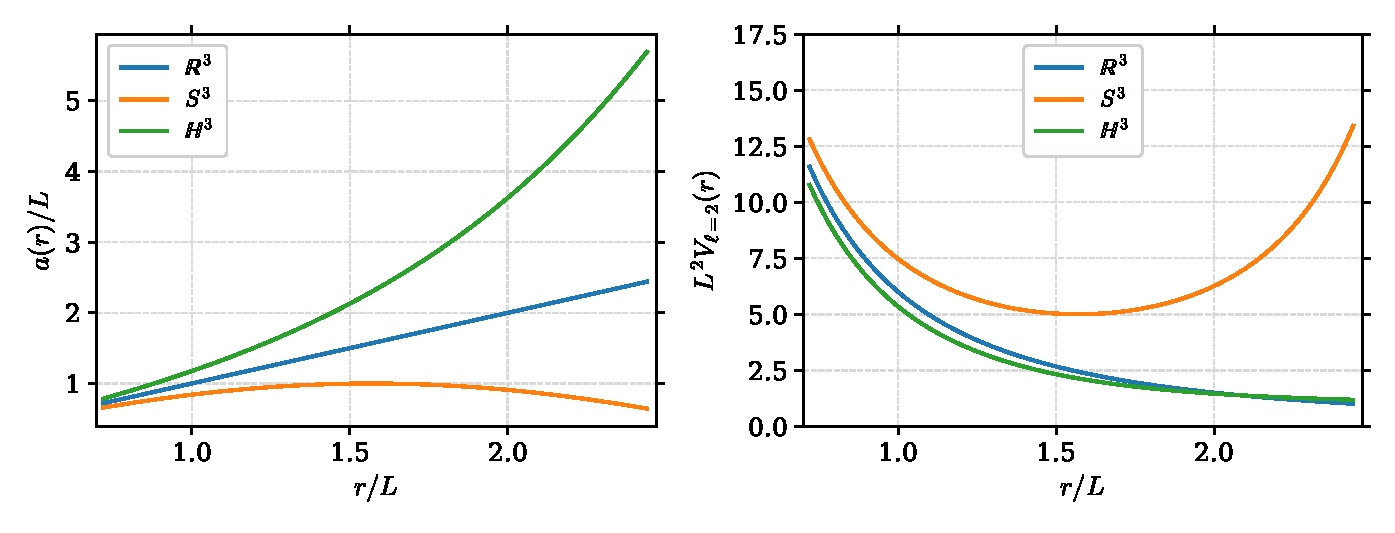
\includegraphics[width=.92\linewidth]{content/MathSkills/figures/geometry-highspin/warped_radial_potentials.pdf}
\caption{同一角动量 $\ell=2$ 在三种三维常曲率空间中的翘曲尺度及酉约化势，均采用 $L=1$。靠近 $r=0$，三者具有相同的 $\ell(\ell+1)/r^2$ 主导奇性；远离原点才可识别不同曲率。图的 $r$ 范围没有延伸到 $S^3$ 的第二极点 $\pi L$。}\label{fig:ghs-r9-warp-potentials}
\end{figure}

\cref{fig:ghs-r9-warp-potentials} 对比了两个不同来源的效应：改变 $a(r)$ 会改变角向面积膨胀；$a''/a$ 则直接给出曲率位移。取 $\ell=0$ 时可再作一个独立的谱核验：在 $S^3$ 上 $u(r)=\sin(r/L)$ 满足两端正则条件并有 $H_0u=0$，对应原始标量 拉普拉斯算子 的常数零模；在 $\mathbb H^3_L$ 上 $V_{0,-}=L^{-2}$，无穷远端是连续谱的阈值，而不是一个可归一化的常数本征态。

对 $S^3$，选定 $\ell\ge0$，引入 $x=r/L$ 与 $n\ge\ell$ 的整数。正则径向解可以写成
\[
 u_{n\ell}(r)=\sin^{\ell+1}x\,C_{n-\ell}^{(\ell+1)}(\cos x),
\]
其中 $C_k^{(\alpha)}$ 是 Gegenbauer 多项式。将 $u=\sin^{\ell+1}x F(\cos x)$ 代入一维方程，利用 $z=\cos x$、$\dd z/\dd x=-\sin x$ 并整理同次幂，可得
\[
 (1-z^2)F''-(2\ell+3)zF'+(n-\ell)(n+\ell+2)F=0.
\]
这是参数 $\alpha=\ell+1$、次数 $n-\ell$ 的 Gegenbauer 方程。

它的多项式解在 $x=0,\pi$ 都正则，且
\[
 H_\ell u_{n\ell}=\frac{n(n+2)}{L^2}u_{n\ell}.
\]
对同一个 $n$，$\ell=0,1,\ldots,n$，每个 $\ell$ 有 $2\ell+1$ 个磁量子数，因而总简并度
\[
 \sum_{\ell=0}^{n}(2\ell+1)=(n+1)^2.
\]
此简并度既由径向边界条件与球谐分解得到，也同 $S^3$ 上标量 拉普拉斯算子 的 $SO(4)$ 表示论结果一致。

它不意味着一般紧致三维流形具有相同简并。

圆锥提供了把几何与径向量子化联系起来的最直接例子，但它也提醒我们：即使截面的谱已经全部算出，径向算子在锥尖处仍可能没有唯一的量子实现。这个问题不能靠“解在原点有限”一句话处理，因为在奇异几何上，平方可积、正则、有限能量及自伴边界条件并不是同一个要求。

令 $g=\dd r^2+r^2h$，$\Sigma$ 维数为 $d-1$，取 $-\Delta_hu_j=\lambda_ju_j$、$\lambda_j\geq0$，并考虑最小耦合 拉普拉斯算子 $-\Delta_g$。
在模态 $\phi=f_j(r)u_j(y)$ 上，由 \cref{eq:ghs-cone-laplace} 得
\begin{equation}\label{eq:ghs-cone-radial-sturm-liouville}
 -f_j''-\frac{d-1}{r}f_j'+\frac{\lambda_j}{r^2}f_j=E f_j.
\end{equation}
径向测度是 $r^{d-1}\dd r$。令 $f_j=r^{-(d-1)/2}v_j$，此替换把该测度准确地变成 $\dd r$，故是 Hilbert 空间的酉变换，而不只是消除一阶导数的技巧。

\begin{proposition}[逆平方径向算子]
在上述酉变换下，\cref{eq:ghs-cone-radial-sturm-liouville} 等价于
\begin{equation}\label{eq:ghs-inverse-square-radial}
 H_{\nu_j}v_j=Ev_j,
 \quad H_\nu=-\frac{\dd^2}{\dd r^2}+\frac{\nu^2-1/4}{r^2},
 \quad \nu_j^2=\lambda_j+\frac{(d-2)^2}{4}.
\end{equation}
\end{proposition}
\begin{proof}
令 $a=(d-1)/2$，则
\[
 f'=r^{-a}(v'-av/r),\quad
 f''=r^{-a}(v''-2av'/r+a(a+1)v/r^2).
\]
代入径向算子后，$v'$ 系数为 $2a-(d-1)=0$。$r^{-2}v$ 的系数为
\[
 -a(a+1)+(d-1)a+\lambda_j
 =\lambda_j+a(a-1)
 =\lambda_j+\frac{(d-1)(d-3)}4.
\]
另一方面，$\nu_j^2-1/4=\lambda_j+[(d-2)^2-1]/4$，两式相同。径向内积也满足
$\int_0^\infty|f|^2r^{d-1}\dd r=\int_0^\infty|v|^2\dd r$，证明该变换保留谱问题所需的 Hilbert 结构。
\end{proof}

靠近 $r=0$，忽略有限 $E$，方程 $H_\nu v=0$ 的 Frobenius 指数满足
$-\alpha(\alpha-1)+\nu^2-1/4=0$，从而 $\alpha=1/2\pm\nu$。对于 $\nu>0$，两支为
\begin{equation}\label{eq:ghs-inverse-square-indicial}
 v_+(r)\sim r^{1/2+\nu},\qquad v_-(r)\sim r^{1/2-\nu}.
\end{equation}
平方可积性直接由 $\int_0^\epsilon r^{2\alpha}\dd r<\infty$ 当且仅当 $\alpha>-1/2$ 决定。所以 $v_+$ 总可积，$v_-$ 仅在 $\nu<1$ 时可积。

\begin{theorem}[非负逆平方系数的锥尖分类]
\label{thm:ghs-inverse-square-endpoint}
对 $\nu\geq0$ 的 $H_\nu$，初始定义域 $C_c^\infty(0,\infty)$，无穷远端为极限点。锥尖 $r=0$ 在 $\nu\geq1$ 时为极限点，因而不需额外的端点自伴参数；在 $0\leq\nu<1$ 时为极限圆，须选取一个自伴边界条件。$\nu=0$ 的第二独立解变为 $r^{1/2}\log r$。
\end{theorem}
\begin{proof}
上面的平方可积计算证明锥尖可积解的个数：$\nu\geq1$ 时只有一支，$0\leq\nu<1$ 时两支均可积。Weyl 极限点/极限圆理论将这一局部计数与相应二阶 Sturm--Liouville 算子的自伴边界条件个数联系起来。无穷远端在本题实逆平方势下是极限点；可以用非实谱参数时的衰减/增长解并由其 Wronskian 不变性检验。对 $\nu=0$，两指数重合，通过 Frobenius 理论取第二支 $r^{1/2}\log r$，两支仍平方可积。故得所述分类。
\end{proof}

假设 $0<\nu<1$，令
\[
 v(r)=A_vr^{1/2+\nu}+B_vr^{1/2-\nu}+o(r^{1/2+\nu}),
\]
对伴随定义域的函数应将其理解为适当的渐近边界迹。在 $[\epsilon,R]$ 上积分分部，得到
\[
 \langle H_\nu v, u\rangle-\langle v, H_\nu u\rangle
 =\bigl[\overline{u'}v-\overline u v'\bigr]_{\epsilon}^{R}.
\]
令 $R\to\infty$、$\epsilon\to0$，内端配对由系数表示为（依照所取法向符号可能整体取负）
\begin{equation}\label{eq:ghs-inverse-square-boundary-form}
 \mathcal B_0(u,v)=2\nu\bigl(\overline{B_u}A_v-\overline{A_u}B_v\bigr).
\end{equation}
使此反厄密边界型消失的极大一维子空间由一个实参数给出，例如 $B=\kappa A$，$\kappa\in\RR\cup\{\infty\}$。量纲为 $[\kappa]=\mathrm{length}^{2\nu}$。不同 $\kappa$ 给出不同的自伴实现；有些扩张可能支持局域束缚态，并引入几何本身没有的长度尺度。

\begin{figure}[htbp]
 \centering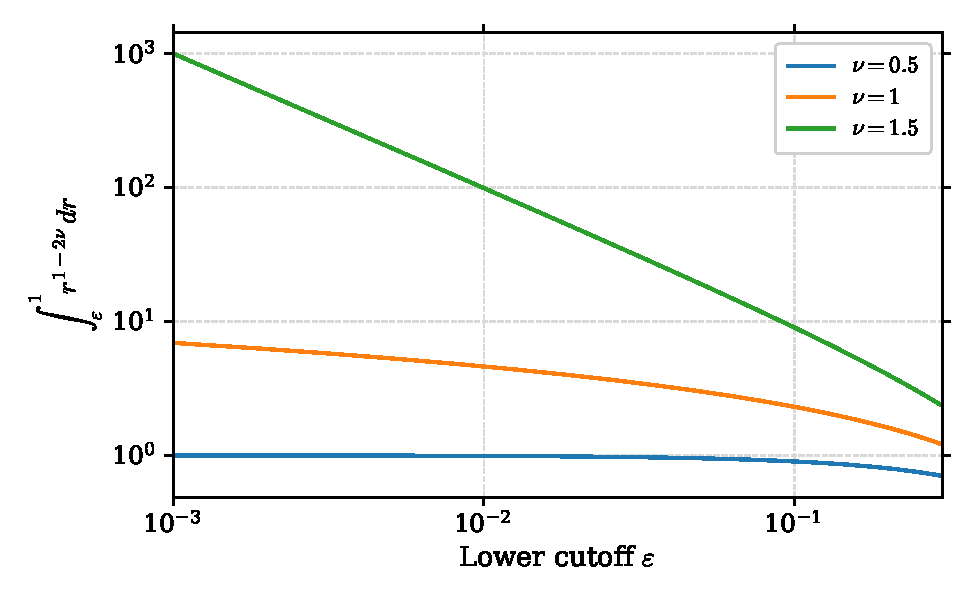
\includegraphics[width=0.77\linewidth]{content/MathSkills/figures/geometry-highspin/conic_boundary_modes.pdf}
 \caption{逆平方径向算子奇异解的截断平方范数。$\nu<1$ 时积分在 $\varepsilon\to0$ 仍有有限极限，$\nu=1$ 呈对数发散，$\nu>1$ 按幂律发散；曲线由 \cref{eq:ghs-inverse-square-indicial} 的幂次精确积分得到。}
 \label{fig:ghs-conic-boundary-norm}
\end{figure}

在平直 $\RR^d$ 去掉原点的 $s$ 波上，$\lambda_0=0$，所以 $\nu_0=(d-2)/2$。当 $d=3$ 时 $\nu_0=1/2<1$，允许非平凡的点相互作用自伴扩张；当 $d=4$ 时 $\nu_0=1$，极限点分类不再给同类单参数族。二维 $d=2$ 时 $\nu_0=0$，必须使用对数支而不是把 $r^{\pm\nu}$ 当作线性独立解。这些结论属于相应径向算子及 Hilbert 空间定义域，而不能被误用为任意相互作用场论的点算符分类。

若圆锥场带曲率耦合 $\xi\mathcal R_g$，则逆平方系数由 $\mathcal R_h$ 改变，且当 $\mathcal R_h$ 不是常数时模态可能发生混合。不能在没有检验这些额外项的情况下直接套用上面的 $\nu_j$。正是这种对定义域与几何条件的明确区分，使任意空间推广具有可检验的数学意义。

抽象谱公式必须通过具体空间检验。不同空间的拓扑、曲率与等距群改变角模态的形式；同一个场算子可以在一种空间上有均匀的角动量阶梯，在另一种空间上只有晶格动量，或者根本不存在方便的显式本征函数。本章固定同一个计算程序，逐次代入不同几何。

取 $\Sigma=S^{d-1}$、单位半径标准度规。曲率 $\mathcal R_h=(d-1)(d-2)$，球谐本征值为 $\lambda_\ell=\ell(\ell+d-2)$。因此
\begin{align}
 A_hY_{\ell a}&=\left[\ell(\ell+d-2)+\frac{(d-2)^2}{4}\right]Y_{\ell a}\nonumber\\
 &=\left(\ell+\frac{d-2}{2}\right)^2Y_{\ell a}.
 \label{eq:ghs-sphere-perfect-square-general}
\end{align}
频率正好是 $\omega_\ell=\ell+\delta$，而不只是它的大 $\ell$ 渐近近似。平方根塌缩成一次函数依赖于圆球曲率与调和谱之间特殊的恒等式。

令球面面积为 $\Omega_{d-1}$、球谐正交归一。对无质量共形标量，柱面两点函数为
\begin{equation}\label{eq:ghs-sphere-cylinder-correlator}
 C(u,\vb n;u',\vb n')
 =\sum_{\ell=0}^\infty\sum_{a=1}^{g_{d,\ell}}
 \frac{\ee^{-(\ell+\delta)|u-u'|}}{2(\ell+\delta)}
 Y_{\ell a}(\vb n)\overline{Y_{\ell a}(\vb n')}.
\end{equation}
将其乘以两端 Weyl 权重 $r^{-\delta}r'^{-\delta}$，回到平直空间时恢复 $|x-x'|^{-(d-2)}$ 类型的二点函数。这个一致性依赖 $d>2$；二维无质量标量具有红外零模和对数关联，不能把 $\delta=0$ 生硬代入振子式。

对严格正的截面算子 $A$，令 $\omega=\sqrt A$。全实直线上的柱体算子 $-\partial_u^2+A$ 有逆核
\begin{equation}\label{eq:math-ghs-positive-cylinder-kernel}
 C_A(u,u')=\frac{\exp[-|u-u'|\sqrt A]}{2\sqrt A}.
\end{equation}
这是谱定理给出的逐模逆算子：对 $Au_j=\lambda_ju_j$，核为
\[
 C_A(u,y;u',y')=\sum_j\frac{e^{-\sqrt{\lambda_j}|u-u'|}}{2\sqrt{\lambda_j}}
 u_j(y)\overline{u_j(y')}.
\]
每一项在 $u\ne u'$ 时解齐次方程，一阶导数在 $u=u'$ 的跃变为 $-1$，故产生单位 $\delta(u-u')$ 源。零模必须单独处理，负谱不能给出这种衰减正核。该逆核作为自由量子场协方差的解释见《自由电子量子光学》的几何自由场章节。

取 $(d-1)$ 维平直环面 $T^{d-1}=\RR^{d-1}/(L_1\ZZ\oplus\cdots\oplus L_{d-1}\ZZ)$，体积 $V=\prod_aL_a$，用周期坐标 $y^a$。归一化本征函数和谱为
\begin{equation}\label{eq:ghs-torus-spectrum}
 u_{\vb k}(y)=V^{-1/2}\ee^{\ii\sum_a2\pi k_ay^a/L_a},\quad
 -\Delta_hu_{\vb k}=\left(\sum_a\frac{4\pi^2k_a^2}{L_a^2}\right)u_{\vb k},\quad \vb k\in\ZZ^{d-1}.
\end{equation}
若加入正质量 $m_0>0$，频率是 $\omega_{\vb k}=\sqrt{m_0^2+\sum_a(2\pi k_a/L_a)^2}$。协方差由 \eqnrefs{eq:math-ghs-positive-cylinder-kernel} 立刻得到
\[
 C_T(u,y;u',y')=\frac1V\sum_{\vb k\in\ZZ^{d-1}}
 \frac{\ee^{-\omega_{\vb k}|u-u'|+\ii\sum_a2\pi k_a(y^a-y'^a)/L_a}}{2\omega_{\vb k}}.
\]
现在模态由整数晶格向量标记。其简并来自格点的长度相等，而非 $SO(d)$ 高自旋表示。若 $L_a$ 一般互不相等，除 $\vb k\leftrightarrow-\vb k$ 外通常没有球面式的大简并。

设 $\Sigma$ 为维数 $d-1$ 的紧致负 Einstein 截面，$\mathcal R_h<0$。常数模 $u_0=V^{-1/2}$ 给出
\[
 A_hu_0=\xi_d\mathcal R_hu_0.
\]
当 $d>2$，本征值为负。尽管圆锥上的无质量方程仍能通过 Weyl 协变性转换成柱面方程，该负模不能被解释为有稳定真空的正频振子。若将局部质量项 $m_0^2$ 加到柱面算子，则需要 $m_0^2> -\inf\operatorname{spec}(A_h)$ 才能使用 \eqnrefs{eq:math-ghs-positive-cylinder-kernel}；这改变了原先共形无质量模型，不能称其为同一个共形场论。

\begin{figure}[htbp]
 \centering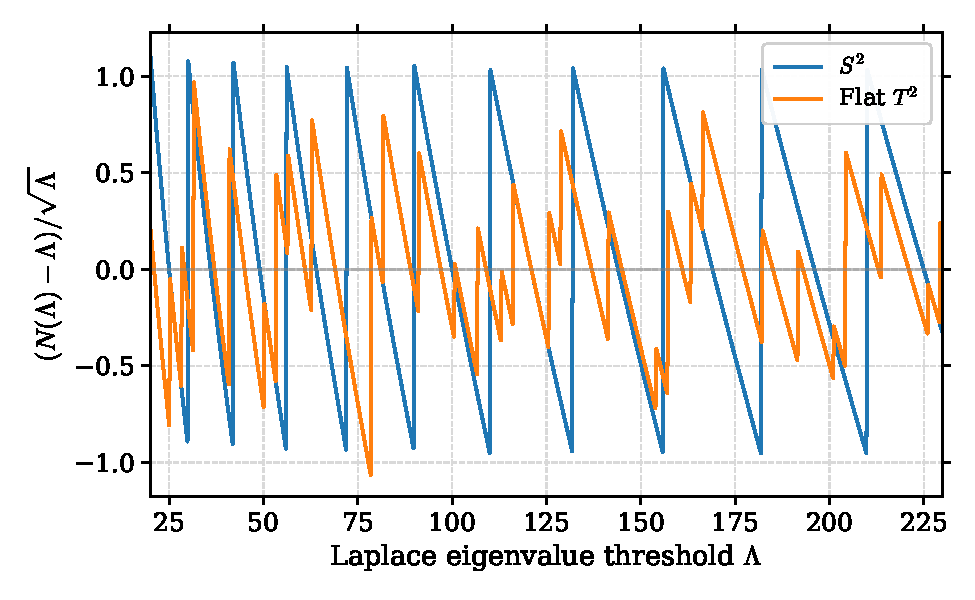
\includegraphics[width=0.78\linewidth]{content/MathSkills/figures/geometry-highspin/sphere_torus_spectral_residual.pdf}
 \caption{面积同为 $4\pi$ 的单位二球面与正方形平直环面之谱计数阶梯，减去相同的 Weyl 主项 $N(\Lambda)\sim\Lambda$ 后除以 $\sqrt\Lambda$。球面的大简并产生较规则的阶梯，环面的格点计数呈另一种振荡；两者有相同领先态密度，却没有相同的精确谱。}
 \label{fig:ghs-sphere-torus-residual}
\end{figure}

取正弦翘曲积
$g=\dd r^2+R^2\sin^2(r/R)\,\dd\Omega_{d-1}^2$，$0<r<\pi R$。它是圆球去掉两极后的度规；两个端点的球面会塌缩，不能用同一组固定截面来构造整个紧致球上的全局圆柱时间。局部变量 $u=\log\tan(r/(2R))$ 给出
\[
 \sin(r/R)=\frac1{\cosh u},\qquad
 g=\frac{R^2}{\cosh^2u}(\dd u^2+\dd\Omega_{d-1}^2).
\]
该几何与柱面共形相关，而不是等距相同。对于质量为零且采用共形耦合的经典标量，Weyl 协变性使柱面算子仍可对角化；量子关联函数还需指定在紧致球两端的正则条件与 Weyl 异常处方。

将这一特殊翘曲函数代回度规，便得到相应的柱面坐标。
由 $u=\log\tan(r/(2R))$ 求导，
\[
 \frac{\dd u}{\dd r}=\frac1{R\sin(r/R)},\qquad
 \dd r=R\sin(r/R)\dd u.
\]
因此 $\dd r^2+R^2\sin^2(r/R)\dd\Omega^2=R^2\sin^2(r/R)(\dd u^2+\dd\Omega^2)$。再使用
$\tan(r/(2R))=\ee^u$ 与 $\sin(2\arctan z)=2z/(1+z^2)$，得到
$\sin(r/R)=2\ee^u/(1+\ee^{2u})=1/\cosh u$。将系数代回即得所列度规。由此可见球面两极在柱面上分别位于 $u\to\mp\infty$。

对于任何给定的紧致截面，先选定 $h$、场所处向量丛、相关二次型及算子定义域；随后求自伴实现 $A$ 的谱或谱测度，并检查其下界。若存在等距群，则优先把 Hilbert 空间按不可约表示分块以简化 $A$；若不齐性则用有限元、谱方法或热核渐近求解。最后根据 \eqnrefs{eq:math-ghs-positive-cylinder-kernel} 构造自由关联函数。只有当几何还提供守恒的尺度生成元和合适的局域算符扇区时，才把该谱进一步解释为共形维数。

\subsection{分离变量的前提}

若 $g=\dd r^2+a(r)^2h$ 且 $A_hu_j=\lambda_ju_j$，对 $\phi(r,y)=f_j(r)u_j(y)$ 代入
$(-\Delta_g+m^2+\xi\mathcal R_g)\phi=0$，得到
\[
 -f_j''-(d-1)\frac{a'}a f_j'
 +\left(\frac{\lambda_j-\xi\mathcal R_h}{a^2}
 +m^2+\xi\mathcal R_g\right)f_j=0,
\]
其中使用 $-\Delta_hu_j=(\lambda_j-\xi\mathcal R_h)u_j$ 要求 $\mathcal R_h$ 为常数；若其不是常数，必须改用 $-\Delta_h$ 的本征基来做 Laplace 分离，或者在相应基底内保留曲率势矩阵。即使可以分离变量，端点附近的正规条件也关系到径向微分算子的自伴实现。

\subsection{算符与量纲}

若物理截面为 $R^2h$，本征值缩放为 $\lambda_j^{\rm phys}=R^{-2}\lambda_j$，真实频率为 $\Omega_j=c\sqrt{\lambda_j}/R$（无量纲 $\lambda_j$ 包含正质量/曲率项）。量子能量激发为 $\hbar\Omega_j$。这与圆柱谱的单位恢复完全一致；但在随时间变化的空间中，不可用单个 $\Omega_j$ 标记全程的能量本征态。

\section{柱体边界响应与拼接}

现在令 $\Sigma$ 为紧致无边界截面，$B\ge0$ 为其上自伴椭圆算子，在有限柱体 $[0,L]\times\Sigma$ 上考虑
\begin{equation}\label{eq:ghs-r6-cylinder-elliptic}
(-\partial_t^2+B)u=0,\qquad u(0)=f_0,\quad u(L)=f_L.
\end{equation}
边界值虽然只落在两张超曲面上，却已经决定了内部的经典场。这说明边界作用量能够编码内部传播；相应的线性算子是 Dirichlet--to--Neumann 映射。


\begin{theorem}[有限柱体的精确边界算子]\label{thm:ghs-r6-cylinder-dn}
在 $B$ 的严格正谱上，外法向边界数据 $(-\partial_tu(0),\partial_tu(L))$ 等于
\begin{equation}\label{eq:ghs-r6-dn-matrix}
\begin{pmatrix}\sqrt B\coth(L\sqrt B)&-\sqrt B\operatorname{csch}(L\sqrt B)\\
-\sqrt B\operatorname{csch}(L\sqrt B)&\sqrt B\coth(L\sqrt B)\end{pmatrix}
\begin{pmatrix}f_0\\f_L\end{pmatrix}.
\end{equation}
零本征子空间上的同一矩阵按连续极限解释为 $L^{-1}\begin{psmallmatrix}1&-1\\-1&1\end{psmallmatrix}$。该映射对称且非负。
\end{theorem}
\begin{proof}
取 $Bu_j=\lambda_ju_j$，写 $u(t,y)=\sum_jq_j(t)u_j(y)$。对 $\lambda_j>0$ 令 $\omega_j=\sqrt{\lambda_j}$，边值常微分方程 $-q_j''+\omega_j^2q_j=0$ 的唯一解为
\[
q_j(t)=\frac{\sinh[\omega_j(L-t)]}{\sinh(\omega_jL)}f_{0j}
+\frac{\sinh(\omega_jt)}{\sinh(\omega_jL)}f_{Lj}.
\]
分别对 $t$ 求导并取端点，得到
\[
-q'_j(0)=\omega_j\coth(\omega_jL)f_{0j}
-\omega_j\operatorname{csch}(\omega_jL)f_{Lj},
\]
\[
q'_j(L)=-\omega_j\operatorname{csch}(\omega_jL)f_{0j}
+\omega_j\coth(\omega_jL)f_{Lj}.
\]
再由谱演算重组为矩阵式。$\omega_j\to0$ 时 $q_j$ 变成端点的线性插值，故零模矩阵具有所给极限。将方程乘以 $\bar u$ 积分分部得到
\[
\langle \Lambda_L(f_0,f_L),(f_0,f_L)\rangle
=\int_0^L\!\bigl(\norm{\partial_tu(t)}^2+\langle Bu(t), u(t)\rangle\bigr)\dd t\ge0,
\]
从而非负性与对称性均可直接验证。严格连续边界算子应理解为适当的 Sobolev 迹空间之间的映射；上述模态计算先在有限谱截断上成立，再由闭二次型扩张。
\end{proof}

离散化后的高斯路径积分把内部变量消去，正是对二次型取 Schur 补；而这里的连续精确边界算子给出了这个代数步骤的几何含义。不同的边界条件会改变谱和高斯归一化，故“内部积分掉了，所以只剩同一个有效作用量”的说法一般不成立。

几何算子提供了谱、逆核和边界二次型；当场论还具有时空对称性，下一章的 Noether 理论才将这些微分结构联系到守恒荷。

\chapter{Poincaré 对称性与 Noether 定理} \label{chap:math-spacetime}

物理学的核心信条之一是：对称性决定守恒律。一个系统如果在空间平移下不变，就拥有动量守恒；如果在时间平移下不变，就拥有能量守恒；如果在旋转下不变，就拥有角动量守恒。Noether 定理把这一直觉提升为精确的数学命题：每一个连续对称性对应一个守恒流。在非相对论力学中，这只涉及 Galilei 群的三维平移和三维旋转。一旦进入相对论，时空统一为四维 Minkowski 流形，对称群变为 Poincaré 群 $ISO(1,d-1)$，它同时包含 Lorentz 变换（旋转和 推进）与四维平移。Poincaré 群的结构比 Galilei 群更丰富，也比纯旋转群更复杂——它是一个半直积，平移子群与 Lorentz 子群之间有非平凡的交织。

前面的代数与几何章节建立了群、表示论、Clifford 代数和几何谱的语言。本章把这些工具汇合于一个物理问题：Poincaré 群如何支配平直时空中的场论。路线图是这样的。首先从 Poincaré 群的群乘法读出它的半直积结构，再通过 Lie 代数把有限变换的无穷小生成元 $P^\mu$（平移）和 $M^{\mu\nu}$（Lorentz）的交换关系一次性导出。然后问：一个物理场 $\Phi^A(x)$ 在 Poincaré 变换下如何变化？答案把场的变换分成两部分——时空坐标移动带来的"轨道"部分和场分量本身在内部表示中旋转的"内禀"部分。有了场的变换律，就可以把它代入作用量变分，Noether 定理自动给出能动量张量和角动量流的守恒方程。最后，Belinfante--Rosenfeld 改进把自旋流吸收进对称的能动量张量，为下一章的曲率时空推广做好准备。

\section{记号与约定}

在进入群结构之前，先固定整套记号。度规符号的选取、生成元的归一化以及无穷小展开的约定，会在后续每一步推导中反复出现；只要其中一项前后不一致，结构常数的符号或 $i$ 因子就会出错。

在 $d$ 维 Minkowski 时空中取度量
\begin{equation*}\eta_{\mu\nu}=\operatorname{diag}(-,+,\ldots,+),\qquad \mu,\nu=0,\ldots,d-1.
\end{equation*}
这里选"多为正"符号约定，即时间分量负、空间分量正。这个选取在广义相对论和粒子物理中都很常见；它的好处是空间度规正定，三维 Euclidean 几何的公式可以直接继承。升降指标均由 $\eta_{\mu\nu}$ 完成，例如 $V^\mu=\eta^{\mu\nu}V_\nu$，$V_0=-V^0$，$V_i=V^i$。全文使用自然单位 $\hbar=c=1$。

Poincaré 群在量子态空间上的表示是酉算符。无穷小展开约定为
\begin{equation}\label{eq:ms-poincare-U-expand}
\boxed{
U(1+\omega,\epsilon)=I+i\epsilon_\mu P^\mu-\frac{i}{2}\omega_{\mu\nu}M^{\mu\nu}+O(\epsilon^2,\omega^2),
}
\end{equation}
其中 $P^\mu$ 是平移生成元（物理上是四动量算符），$M^{\mu\nu}=-M^{\nu\mu}$ 是 Lorentz 生成元（物理上是角动量算符，包含空间旋转和 推进）。三个细节值得解释。第一，因子 $i$ 使 $P^\mu$ 和 $M^{\mu\nu}$ 成为 Hermite 算符，从而对应物理可观测量。第二，$\omega_{\mu\nu}$ 的反对称性 $\omega_{\mu\nu}=-\omega_{\nu\mu}$ 保证只有 $d(d-1)/2$ 个独立 Lorentz 参数（$d=4$ 时是 6 个：3 个旋转加 3 个 推进），而求和中的 $1/2$ 补偿了每对 $(\mu,\nu)$ 被计算两次。第三，平移参数 $\epsilon^\mu$ 是一个 $d$-矢量，没有反对称约束。

\section{Poincaré 群及其 Lie 代数}
物理上，Poincaré 变换是保持 Minkowski 间隔 $\dd s^2=\eta_{\mu\nu}\dd x^\mu \dd x^\nu$ 不变的最一般仿射变换。它由一个 Lorentz 矩阵 $\Lambda$ 和一个平移矢量 $a$ 组成：
\begin{equation*}x'^\mu=\Lambda^\mu{}_\nu x^\nu+a^\mu.
\end{equation*}
Lorentz 矩阵必须满足
\begin{equation}\label{eq:ms-poincare-lorentz-def}
\boxed{\Lambda^T\eta\Lambda=\eta,}
\end{equation}
即 $\eta_{\rho\sigma}\Lambda^\rho{}_\mu\Lambda^\sigma{}_\nu=\eta_{\mu\nu}$。这个条件的几何意义是：$\Lambda$ 保持 Minkowski 内积不变。物理上，它保证光锥结构不变——如果两个事件由光信号连接（$\dd s^2=0$），变换后仍然如此。
群乘法告诉我们连续做两次 Poincaré 变换的净效果。设 $g_1=(\Lambda_1,a_1)$ 和 $g_2=(\Lambda_2,a_2)$。先做 $g_1$：$x'=\Lambda_1 x+a_1$；再做 $g_2$：$x''=\Lambda_2 x'+a_2$。代入得
\begin{equation}
x''=\Lambda_2\Lambda_1 x+(\Lambda_2 a_1+a_2).
\end{equation}
因此群乘法为
\begin{equation}\label{eq:ms-poincare-semidirect}
\boxed{
(\Lambda_2,a_2)(\Lambda_1,a_1)=(\Lambda_2\Lambda_1,\;\Lambda_2 a_1+a_2).
}
\end{equation}
关键观察：平移部分出现的是 $\Lambda_2 a_1$ 而非 $a_1$。这意味着先平移再 Lorentz 变换，与先 Lorentz 变换再平移，效果不同——Lorentz 变换会"搅动"平移矢量。这正是半直积的特征：
\begin{equation}
ISO(1,d-1)=SO(1,d-1)\ltimes\mathbb{R}^{1,d-1}.
\end{equation}
如果是直积，群乘法会是 $(\Lambda_2\Lambda_1,\;a_2+a_1)$，两个子群完全独立。半直积中的 $\ltimes$ 记号正是记录了 Lorentz 对平移的非平凡作用。这个结构会在下一步直接进入 Lie 代数的交换关系：$[M,P]\neq 0$。
逆元公式在推导 Lie 括号 时会用到。令 $(\Lambda,a)^{-1}=(\Lambda',a')$，要求 $(\Lambda',a')(\Lambda,a)=(I,0)$。由群乘法\eqnrefs{eq:ms-poincare-semidirect} 得 $(\Lambda'\Lambda,\;\Lambda'a+a')=(I,0)$。第一分量给出 $\Lambda'=\Lambda^{-1}$；代入第二分量给出 $a'=-\Lambda^{-1}a$。因此
\begin{equation}\label{eq:ms-poincare-inverse}
(\Lambda,a)^{-1}=(\Lambda^{-1},\;-\Lambda^{-1}a).
\end{equation}
注意平移部分的逆元不是 $-a$ 而是 $-\Lambda^{-1}a$——又是半直积的体现。

\section{Poincaré 代数的统一推导}

有了群结构，下一步问：为什么要把群变成 Lie 代数？原因是群乘法是非线性的，而 Lie 代数的交换关系是线性的结构常数，后者远比前者容易操作。无穷小生成元的交换关系 $[P,P]$、$[M,P]$、$[M,M]$ 完全编码了群的局域结构，而且可以用来构造 Casimir 不变量、分类不可约表示、验证场方程的协变性。本节不直接列出这三组公式，而是从群乘法和 Lie 括号 的定义出发，用一个统一的推导一次性得到全部三组关系。
先单独看 Lorentz 部分。取恒等元附近 $\Lambda=I+\omega+O(\omega^2)$，其中 $\omega$ 是无穷小矩阵。代入 Lorentz 条件\eqnrefs{eq:ms-poincare-lorentz-def}：
\begin{equation*}
(I+\omega)^T\eta(I+\omega)=\eta.
\end{equation*}
展开到一阶：
\begin{equation*}
\eta+\omega^T\eta+\eta\omega+O(\omega^2)=\eta,
\end{equation*}
故
\begin{equation}
\omega^T\eta+\eta\omega=0.
\end{equation}
这个条件说 $\omega$ 关于 $\eta$ 反对称。为了把矩阵条件转成分量条件，定义降指标版本 $\omega_{\mu\nu}=\eta_{\mu\rho}\omega^\rho{}_\nu$。那么
\begin{equation}
\omega_{\nu\mu}=\eta_{\nu\rho}\omega^\rho{}_\mu=\eta_{\nu\rho}\eta_{\mu\sigma}\omega^\sigma{}_\nu\cdot(\text{转置})=-\eta_{\mu\rho}\omega^\rho{}_\nu=-\omega_{\mu\nu},
\end{equation}
即
\begin{equation*}\boxed{\omega_{\mu\nu}=-\omega_{\nu\mu}.}
\end{equation*}
$d\times d$ 反对称矩阵有 $d(d-1)/2$ 个独立分量，这就是 Lorentz 群的维数。在 $d=4$ 时，6 个生成元分为 3 个旋转 $J_i=\frac{1}{2}\epsilon_{ijk}M^{jk}$ 和 3 个 推进 $K_i=M^{0i}$。
现在进入核心推导。Poincaré Lie 代数的元素写成 $X=(\omega,a)$，其中 $\omega\in\mathfrak{so}(1,d-1)$ 是反对称矩阵，$a\in\mathbb{R}^{1,d-1}$ 是平移矢量。Lie 括号 的一般定义是通过群交换子：
\begin{equation}\label{eq:ms-poincare-bracket-def}
g_1(t)g_2(s)g_1(t)^{-1}g_2(s)^{-1}=I+ts\,[X_1,X_2]+O(t^2,s^2,t^2s,ts^2),
\end{equation}
其中 $g_1(t)=(e^{t\omega_1},ta_1)$ 和 $g_2(s)=(e^{s\omega_2},sa_2)$ 是两条一参数子群。群交换子的几何意义是：先沿 $g_1$ 走一小段 $t$，再沿 $g_2$ 走一小段 $s$，然后沿 $g_1$ 退回，再沿 $g_2$ 退回。如果群是 Abel 的，这四步完全抵消；非抵消的部分到 $ts$ 阶正是 Lie 括号，它测量两个生成元"不交换"的程度。

这条统一的 括号 公\eqnrefs{eq:ms-poincare-unified-bracket} 是整个 Poincaré 代数的压缩形式。它的两个分量分别给出：Lorentz 部分的矩阵交换子 $[\omega_1,\omega_2]$（纯 Lorentz 子代数），以及平移部分的 $\omega_1 a_2-\omega_2 a_1$（Lorentz 对平移的交叉作用）。下面三小节只需在\eqnrefs{eq:ms-poincare-unified-bracket} 中代入不同的特例，即可一次性得到全部三组交换关系。
纯平移对应 $\omega_1=\omega_2=0$。代入\eqnrefs{eq:ms-poincare-unified-bracket}：
\begin{equation*}
[(0,a_1),(0,a_2)]=\big([0,0],\;0\cdot a_2-0\cdot a_1\big)=(0,0).
\end{equation*}
两个纯平移的 括号 为零，因为 Lorentz 部分恒为零、交叉项中 $\omega=0$ 也为零。翻译成生成元语言：
\begin{equation}\label{eq:ms-poincare-PP}
\boxed{[P_\mu,P_\nu]=0.}
\end{equation}
这反映平移子群 $\mathbb{R}^{1,d-1}$ 是 Abel 群——先沿 $x^\mu$ 方向平移再沿 $x^\nu$ 方向平移，与顺序无关。
取一个纯 Lorentz 元素 $X_1=(\omega,0)$ 和一个纯平移元素 $X_2=(0,a)$。代入\eqnrefs{eq:ms-poincare-unified-bracket}：
\begin{equation*}
[(\omega,0),(0,a)]=\big([\omega,0],\;\omega a-0\cdot 0\big)=(0,\omega a).
\end{equation*}
结果是一个纯平移元素，平移矢量被 $\omega$ 作用。物理上，这说 Lorentz 变换会把一个平移矢量旋转或 推进 到另一个方向。在生成元语言中，Lorentz 生成元对平移生成元的伴随作用正是矢量表示。为了写出显式公式，需要把矩阵 $\omega$ 用反对称参数 $\omega_{\rho\sigma}$ 和矢量表示的 Lorentz 生成元 $J_V^{\rho\sigma}$ 展开。矢量表示的定义是：对任意矢量 $a$，$(\omega a)^\mu=\omega^\mu{}_\nu a^\nu$。由 $\omega^\mu{}_\nu=\eta^{\mu\alpha}\omega_{\alpha\nu}$ 和 $\omega_{\alpha\nu}$ 的反对称性，
\begin{equation*}
(\omega a)^\mu=\eta^{\mu\alpha}\omega_{\alpha\nu}a^\nu=\frac{1}{2}\omega_{\rho\sigma}\big(\eta^{\rho\mu}\delta^\sigma{}_\nu-\eta^{\sigma\mu}\delta^\rho{}_\nu\big)a^\nu.
\end{equation*}
因此矢量表示的 Lorentz 生成元为
\begin{equation}\label{eq:ms-poincare-JV}
\boxed{
(J_V^{\rho\sigma})^\mu{}_\nu=i\big(\eta^{\rho\mu}\delta^\sigma{}_\nu-\eta^{\sigma\mu}\delta^\rho{}_\nu\big),
}
\end{equation}
其中因子 $i$ 是为了与量子力学中 Hermite 生成元的约定一致。于是 $[M^{\rho\sigma},P^\mu]$ 必须按同一矢量表示作用：
\begin{equation}\label{eq:ms-poincare-MP}
\boxed{
[M^{\rho\sigma},P^\mu]=-i\big(\eta^{\rho\mu}P^\sigma-\eta^{\sigma\mu}P^\rho\big).
}
\end{equation}
物理含义：Lorentz 生成元把平移生成元变为相应矢量分量。
这里的负号与 $J_V=i(\eta\delta-\eta\delta)$、$L=i(x\partial-x\partial)$ 一致；
例如空间子代数直接给出 $[J_V^{12},J_V^{23}]=iJ_V^{13}$。
若改选相反号的 Lorentz 生成元，$[M,M]$ 与 $[M,P]$ 都须同时改号，不能混用。这就是半直积在 Lie 代数中的表现——$[M,P]\neq 0$。
最后取两个纯 Lorentz 元素 $X_1=(\omega_1,0)$ 和 $X_2=(\omega_2,0)$。代入\eqnrefs{eq:ms-poincare-unified-bracket}：
\begin{equation*}
[(\omega_1,0),(\omega_2,0)]=\big([\omega_1,\omega_2],\;\omega_1\cdot 0-\omega_2\cdot 0\big)=\big([\omega_1,\omega_2],\,0\big).
\end{equation*}
平移部分为零，结果仍是纯 Lorentz 元素。Lorentz 子代数在 Poincaré 代数中是子代数（不是理想，因为 $[M,P]\neq 0$）。现在需要把矩阵交换子 $[\omega_1,\omega_2]$ 翻译成生成元 $M^{\mu\nu}$ 的交换关系。在矢量表示中，$(J^{\mu\nu})^\rho{}_\sigma=i(\eta^{\mu\rho}\delta^\nu{}_\sigma-\eta^{\nu\rho}\delta^\mu{}_\sigma)$。

由于 Lie 代数的结构常数与具体忠实表示无关（这是 Lie 理论的基本定理：同一个抽象 Lie 代数的任何两个忠实表示给出相同的结构常数），矢量表示中得到的交换关系对一般 Lorentz 生成元 $M^{\mu\nu}$ 同样成立：
\begin{equation}\label{eq:ms-poincare-MM}
\boxed{
[M^{\mu\nu},M^{\rho\sigma}]=-i\big(\eta^{\mu\rho}M^{\nu\sigma}-\eta^{\mu\sigma}M^{\nu\rho}-\eta^{\nu\rho}M^{\mu\sigma}+\eta^{\nu\sigma}M^{\mu\rho}\big).
}
\end{equation}
\eqnrefs{eq:ms-poincare-PP}、\eqnrefs{eq:ms-poincare-MP}、\eqnrefs{eq:ms-poincare-MM} 合起来构成 Poincaré Lie 代数。三条关系全部由统一的半直积 Lie 括号\eqnrefs{eq:ms-poincare-unified-bracket} 一次性导出，这正是统一推导的优势：不需要分别猜三组公式的右端，一个群结构给出全部。

物理上，这三条关系有清晰的含义。$[P,P]=0$ 说不同方向的平移互不干扰。$[M,P]\neq 0$ 说 Lorentz 变换会把平移方向旋转到新方向——这就是为什么能量（$P^0$）和动量（$P^i$）在 推进 下会混合。$[M,M]\neq 0$ 说两个旋转的合成一般不是简单相加——例如绕 $x$ 轴旋转再绕 $y$ 轴旋转，与反过来做，结果差一个绕 $z$ 轴的旋转。

\section{Poincaré 群在场上的表示}
到目前为止，$P^\mu$ 和 $M^{\mu\nu}$ 是作用在量子态空间上的抽象算符。但在场论中，基本对象不是态矢量而是场 $\Phi^A(x)$——一组时空依赖的分量，$A$ 标记内部自由度。物理上，场可以是标量（如 Higgs 场 $\phi(x)$）、矢量（如电磁势 $A_\mu(x)$）、旋量（如 Dirac 场 $\psi_\alpha(x)$）等。当坐标系做 Poincaré 变换时，场不仅因为坐标移动而改变（"被动"效应），还因为自身分量在内部空间中旋转而改变（"主动"效应）。后者正是 Lorentz 群的有限维表示 $D(\Lambda)$。
采用被动约定：坐标变换 $x\to x'=\Lambda x+a$ 下，场的变换律为
\begin{equation}\label{eq:ms-poincare-field-transform}
\boxed{
U(\Lambda,a)\Phi^A(x)U^{-1}(\Lambda,a)=D(\Lambda^{-1})^A{}_B\,\Phi^B(\Lambda x+a).
}
\end{equation}
右边有两个因素。$\Phi^B(\Lambda x+a)$ 是坐标移动带来的——场在新坐标处的值。$D(\Lambda^{-1})^A{}_B$ 是内部表示矩阵——场分量本身在 Lorentz 变换下的旋转。注意是 $\Lambda^{-1}$ 而非 $\Lambda$，这是被动变换的约定。

$D$ 必须是 Lorentz 群的表示，即 $D(\Lambda_2\Lambda_1)=D(\Lambda_2)D(\Lambda_1)$。原因很简单：连续做两次变换 $\Lambda_1$ 再 $\Lambda_2$，等价于一次 $\Lambda_2\Lambda_1$，表示矩阵必须按同一规则合成。
写 $\Lambda=I+\omega$，一般有限维表示展开为
\begin{equation}\label{eq:ms-poincare-D-expand}
D(I+\omega)=I-\frac{i}{2}\omega_{\mu\nu}\Sigma^{\mu\nu},
\end{equation}
其中 $\Sigma^{\mu\nu}=-\Sigma^{\nu\mu}$ 是表示空间上的矩阵（不是量子算符），满足与 $M^{\mu\nu}$ 相同的 Lorentz Lie 代数。因子 $-i/2$ 与\eqnrefs{eq:ms-poincare-U-expand} 一致。

定义位移矢量 $\xi^\mu=\epsilon^\mu+\omega^\mu{}_\nu x^\nu$，它把无穷小 Poincaré 变换的坐标移动写成 $x'^\mu=x^\mu+\xi^\mu$。由 Taylor 展开
\begin{equation*}
\Phi^B(\Lambda x+a)=\Phi^B(x)+\xi^\rho\partial_\rho\Phi^B(x)+O(\xi^2),
\end{equation*}
以及 $D(\Lambda^{-1})=D(I-\omega)=I+\frac{i}{2}\omega_{\mu\nu}\Sigma^{\mu\nu}$，代入\eqnrefs{eq:ms-poincare-field-transform} 得到无穷小场变分
\begin{equation}\label{eq:ms-poincare-delta-Phi}
\boxed{
\delta\Phi^A=\xi^\rho\partial_\rho\Phi^A+\frac{i}{2}\omega_{\mu\nu}(\Sigma^{\mu\nu})^A{}_B\Phi^B.
}
\end{equation}
第一项是轨道部分（坐标移动），第二项是内禀部分（场分量旋转）。
纯 Lorentz 变换（$\epsilon=0$）下，$\xi^\mu=\omega^\mu{}_\nu x^\nu$，场变分为
\begin{equation*}
\delta_\omega\Phi=\omega^\mu{}_\nu x^\nu\partial_\mu\Phi+\frac{i}{2}\omega_{\mu\nu}\Sigma^{\mu\nu}\Phi.
\end{equation*}
右端两项分别来自坐标移动和内部旋转。为了把两者统一在一个生成元下，需要把轨道部分也改写成 $\omega_{\mu\nu}$ 的缩并形式。

合并后，场上的总 Lorentz 生成元自然分为轨道与内禀两部分：
\begin{equation*}\boxed{M^{\mu\nu}_{\text{field}}=L^{\mu\nu}+\Sigma^{\mu\nu}.}
\end{equation*}
这个分解的物理意义非常重要。$L^{\mu\nu}$ 只涉及坐标 $x$ 和导数 $\partial$，与场的内部类型无关——无论是标量、矢量还是旋量，轨道部分都一样。$\Sigma^{\mu\nu}$ 只作用在场的内部指标上，与时空位置无关——标量的 $\Sigma=0$，矢量的 $\Sigma$ 是 $d\times d$ 矩阵，旋量的 $\Sigma$ 是 Clifford 代数构造。不同类型的场，只是选择了不同的 $\Sigma^{\mu\nu}$。

\section{任意阶张量与旋量的 Lorentz 生成元}

上一节把场的 Lorentz 生成元分解为 $M=L+\Sigma$，其中 $\Sigma$ 由场的类型决定。本节逐一计算常见场类型的 $\Sigma^{\mu\nu}$。
标量场是最简单的情形：$\phi'(x')=\phi(x)$，场分量不旋转，$D(\Lambda)=1$。因此
\begin{equation*}
\boxed{\Sigma^{\mu\nu}=0\quad\text{(标量)}.}
\end{equation*}
标量场的 Lorentz 生成元纯轨道：$M^{\mu\nu}=L^{\mu\nu}=i(x^\mu\partial^\nu-x^\nu\partial^\mu)$。

四矢量场 $V^\rho$ 在 Lorentz 变换下按 $V'^\rho=\Lambda^\rho{}_\sigma V^\sigma$ 变换。无穷小形式 $\delta V^\rho=\omega^\rho{}_\sigma V^\sigma$ 应与\eqnrefs{eq:ms-poincare-D-expand} 给出的 $\delta V^\rho=-\frac{i}{2}\omega_{\mu\nu}(\Sigma^{\mu\nu})^\rho{}_\sigma V^\sigma$ 一致。比较 $\omega_{\mu\nu}$ 的系数（注意 $\omega^\rho{}_\sigma=\eta^{\rho\mu}\omega_{\mu\sigma}$）得到
\begin{equation*}\boxed{
(\Sigma^{\mu\nu})^\rho{}_\sigma=i(\eta^{\mu\rho}\delta^\nu{}_\sigma-\eta^{\nu\rho}\delta^\mu{}_\sigma)\quad\text{(矢量)}.
}
\end{equation*}
这与矢量表示的 Lorentz 生成元\eqnrefs{eq:ms-poincare-JV} 一致——这正是预期的，因为矢量场按矢量表示变换。
一般 $(r,s)$ 张量 $T^{\alpha_1\cdots\alpha_r}{}_{\beta_1\cdots\beta_s}$ 有 $r$ 个上指标和 $s$ 个下指标。Lorentz 变换对每一个指标独立作用：每个上指标贡献一个矢量表示的 $\Sigma$，每个下指标贡献一个协变矢量表示的 $\Sigma$。总生成元是各指标生成元之和。显式地：
\begin{equation*}\boxed{
\begin{aligned}
(\Sigma^{\mu\nu}T)^{\alpha_1\cdots\alpha_r}{}_{\beta_1\cdots\beta_s}
={}&i\sum_{k=1}^{r}\Big(\eta^{\mu\alpha_k}T^{\cdots\nu\cdots}{}_{\cdots}-\eta^{\nu\alpha_k}T^{\cdots\mu\cdots}{}_{\cdots}\Big)\\
&+i\sum_{\ell=1}^{s}\Big(\delta^\mu{}_{\beta_\ell}T^{\cdots}{}_{\cdots\nu\cdots}-\delta^\nu{}_{\beta_\ell}T^{\cdots}{}_{\cdots\mu\cdots}\Big),
\end{aligned}
}
\end{equation*}
其中省略号表示未被替换的指标保持不变。例如对二阶逆变张量 $T^{\rho\sigma}$：
\begin{equation*}
(\Sigma^{\mu\nu}T)^{\rho\sigma}=i\big(\eta^{\mu\rho}T^{\nu\sigma}-\eta^{\nu\rho}T^{\mu\sigma}+\eta^{\mu\sigma}T^{\rho\nu}-\eta^{\nu\sigma}T^{\rho\mu}\big).
\end{equation*}
这就是 $\Sigma^{\mu\nu}_{(2)}=\Sigma^{\mu\nu}_{(1)}\otimes I+I\otimes\Sigma^{\mu\nu}_{(1)}$——张量积表示的生成元是各因子生成元之和。
旋量场的 $\Sigma^{\mu\nu}$ 不能从普通张量指标构造，因为旋量不属于任何 $SO(1,d-1)$ 的张量表示。它属于 Lorentz 群的双覆盖 $Spin(1,d-1)$ 的旋量表示。构造旋量表示的出发点是 Clifford 代数
\begin{equation*}\boxed{\{\gamma^\mu,\gamma^\nu\}=2\eta^{\mu\nu},}
\end{equation*}
它要求 $\gamma^\mu$ 是 $2^{\lfloor d/2\rfloor}\times 2^{\lfloor d/2\rfloor}$ 矩阵（$d=4$ 时是 $4\times4$）。旋量表示 $D(\Lambda)$ 必须保持 Clifford 代数协变：
\begin{equation}\label{eq:ms-poincare-clifford-cov}
D^{-1}(\Lambda)\gamma^\rho D(\Lambda)=\Lambda^\rho{}_\sigma\gamma^\sigma.
\end{equation}
这个条件的物理意义是：$\gamma^\mu$ 作为"矢量矩阵"在 Lorentz 变换下应按矢量表示旋转，而 $D(\Lambda)$ 是实现这一旋转的旋量表示矩阵。

因此 Dirac 旋量的 Lorentz 生成元
\begin{equation}\label{eq:ms-poincare-Sigma-dirac}
\boxed{\Sigma^{\mu\nu}=\frac{i}{4}[\gamma^\mu,\gamma^\nu]\quad\text{(Dirac 旋量)}.}
\end{equation}
Dirac 场上的总 Lorentz 生成元
\begin{equation*}\boxed{
M^{\mu\nu}=i(x^\mu\partial^\nu-x^\nu\partial^\mu)+\frac{i}{4}[\gamma^\mu,\gamma^\nu].
}
\end{equation*}
第一项是轨道角动量，第二项是自旋角动量。在 $d=4$ 时，若定义常用的
$\sigma^{\mu\nu}=\frac{\ii}{2}[\gamma^\mu,\gamma^\nu]$，
则 $\Sigma^{\mu\nu}=\sigma^{\mu\nu}/2$。
这两个符号相差因子 $2$，在变换指数中必须保持同一约定。
在 $d=4$ 时，Lorentz 群的双覆盖 $Spin(1,3)\simeq SL(2,\mathbb{C})$。有限维不可约表示由一对半整数 $(j_L,j_R)$ 标记，其中 $j_L,j_R=0,\frac{1}{2},1,\ldots$。这个标记的来源是：Lorentz Lie 代数的复化分解为
$\mathfrak{so}(1,3)_\CC\simeq\mathfrak{sl}_2(\CC)\oplus\mathfrak{sl}_2(\CC)$，
其有限维表示用两份角动量代数来标记；实 Lie 群 $SL(2,\CC)$
并不同构于紧群 $SU(2)\times SU(2)$，每个因子有自己的角动量量子数。常见场的表示对应关系：

\begin{center}
\begin{tabular}{ll}
\hline
场 & Lorentz 表示 \\
\hline
标量 & $(0,0)$ \\
左手 Weyl & $(\frac{1}{2},0)$ \\
右手 Weyl & $(0,\frac{1}{2})$ \\
Dirac & $(\frac{1}{2},0)\oplus(0,\frac{1}{2})$ \\
四矢量 & $(\frac{1}{2},\frac{1}{2})$ \\
自对偶二形式 & $(1,0)$ \\
反自对偶二形式 & $(0,1)$ \\
对称无迹 秩-2 & $(1,1)$ \\
\hline
\end{tabular}
\end{center}

这张表是后续自旋分类的基础。注意 Dirac 旋量是可约表示——它由左手和右手 Weyl 旋量直和而成。质量为零时这两个分量解耦，各自独立描述不同螺旋度的粒子；质量不为零时质量项把它们耦合，这就是下一章要详细讨论的 手征性-螺旋度 关系。

\section{Wigner 分类：场表示与粒子自旋}

到这里有一个必须强调的区别：场的 Lorentz 表示不等于单粒子的 Poincaré 不可约表示。场 $\Phi^A(x)$ 的指标 $A$ 属于有限维 Lorentz 表示，它描述的是场在 Lorentz 变换下的变换律。但物理单粒子态是 Hilbert 空间中的向量，它们按照 Poincaré 群的\emph{无穷维}酉表示分类——Wigner 1939 年的分类方案。同一个场可以产生多种粒子态（例如矢量场 $A_\mu$ 在无质量时只产生 $h=\pm1$ 两个螺旋度的光子，而非 4 个分量对应 4 种粒子）。

Wigner 分类的关键是两个 Casimir 不变量——它们与所有 Poincaré 生成元对易，因此在不可约表示上是常数。第一 Casimir 是
\begin{equation*}\boxed{C_1=P^2=P_\mu P^\mu,}
\end{equation*}
对质量为 $m$ 的粒子给出 $P^2=-m^2$（本文"多为正"度规下）。第二 Casimir 由 Pauli--Lubanski 向量
\begin{equation*}W^\mu=\frac{1}{2}\epsilon^{\mu\nu\rho\sigma}P_\nu M_{\rho\sigma}
\end{equation*}
构造：
\begin{equation*}\boxed{C_2=W^2=W_\mu W^\mu.}
\end{equation*}
对 有质量 自旋-$s$ 粒子，$W^2=m^2 s(s+1)$。无质量粒子则由 小群 分类——有质量 的 小群 是 $SO(3)$，无质量 的是 $ISO(2)$，两者的表示结构截然不同。这些细节留到下一章系统讨论。

\section{最小作用量原理与 Euler--Lagrange 方程}

有了场的变换律，下一步问：什么样的场是物理允许的？经典场论的回答是作用量驻定。考虑一阶局域场论
\begin{equation}
S[\Phi]=\int \dd^dx\,\mathcal{L}(\Phi^A,\partial_\mu\Phi^A),
\end{equation}
其中拉氏密度 $\mathcal{L}$ 依赖于场和它的一阶导数。物理场是使 $\delta S=0$（对边界消失的任意变分）的场。

\section{Noether 第一定理的一般形式}

Noether 定理把连续对称性与守恒律联系起来。核心思想很简单：如果某种连续变换使作用量不变（最多差一个边界项），那么对应的变分恒等式自动给出一个散度为零的流——守恒流。

首先把任意变分写成标准形式。利用 Euler--Lagrange 方程的推导过程，任何变分都可以写成
\begin{equation}\label{eq:ms-poincare-delta-L}
\boxed{
\delta\mathcal{L}=E_A\,\delta\Phi^A+\partial_\mu\Theta^\mu,
}
\end{equation}
其中 $E_A=\frac{\partial\mathcal{L}}{\partial\Phi^A}-\partial_\mu\Pi_A^\mu$ 是 EL 表达式（$E_A=0$ 即运动方程），$\Theta^\mu=\Pi_A^\mu\delta\Phi^A$ 是 Symplectic 势。这个分解的物理意义：变分的效果分为两部分——一部分正比于运动方程（在壳 为零），另一部分是全散度（边界项）。

现在假设某种连续变换使拉氏量的变分是一个全散度：
\begin{equation}
\delta\mathcal{L}=\partial_\mu K^\mu.
\end{equation}
这种变换称为"准对称"（quasi-对称）。例如平移变换使 $\delta\mathcal{L}=\epsilon^\nu\partial_\nu\mathcal{L}=\partial_\mu(\epsilon^\mu\mathcal{L})$，故 $K^\mu=\epsilon^\mu\mathcal{L}$。把\eqnrefs{eq:ms-poincare-delta-L} 与准对称条件结合：
\begin{equation*}
E_A\,\delta\Phi^A+\partial_\mu\Theta^\mu=\partial_\mu K^\mu,
\end{equation*}
即
\begin{equation*}
E_A\,\delta\Phi^A+\partial_\mu(\Theta^\mu-K^\mu)=0.
\end{equation*}
定义 Noether 流
\begin{equation}\label{eq:ms-poincare-J-def}
\boxed{J^\mu=\Theta^\mu-K^\mu=\Pi_A^\mu\delta\Phi^A-K^\mu,}
\end{equation}
则 off-shell 恒等式为
\begin{equation*}\boxed{\partial_\mu J^\mu=-E_A\,\delta\Phi^A.}
\end{equation*}
在运动方程成立时（在壳，$E_A=0$），右端为零：
\begin{equation}\label{eq:ms-poincare-noether}
\boxed{\partial_\mu J^\mu=0\quad\text{(on-shell)}.}
\end{equation}
这就是 Noether 第一定理：每一个连续准对称性给出一个 在壳 守恒流。

\section{Poincaré 对称性与能动量守恒}

\begin{workedexample}[平移不变性与应力能量守恒]
在平直时空取实标量场的密度 \(\mathcal L=\tfrac12\partial_\mu\phi\,\partial^\mu\phi-\tfrac12\kappa^2\phi^2\)，其中 \(\kappa>0\) 为常数。定义 Euler--Lagrange 表达式 \(E(\phi)=\partial\mathcal L/\partial\phi-\partial_\mu[\partial\mathcal L/\partial(\partial_\mu\phi)]\)。验证正则张量 \(T^\mu{}_\nu=\partial^\mu\phi\,\partial_\nu\phi-\delta^\mu{}_\nu\mathcal L\) 的散度恒等式。

\textbf{解.} 先有 \(E(\phi)=-(\Box+\kappa^2)\phi\)。对 \(T^\mu{}_\nu\) 求导并用乘积法则，
\[
\partial_\mu T^\mu{}_\nu
=(\Box\phi)\partial_\nu\phi
+\partial^\mu\phi\,\partial_\mu\partial_\nu\phi
-\partial_\nu\mathcal L.
\]
第二项等于 \(\partial_\nu[\tfrac12\partial_\rho\phi\,\partial^\rho\phi]\)，因此与 \(\partial_\nu\mathcal L\) 中的动能导数抵消，留下
\[
\partial_\mu T^\mu{}_\nu
=(\Box\phi+\kappa^2\phi)\partial_\nu\phi
=-E(\phi)\partial_\nu\phi.
\]
这在任意光滑场上都是恒等式；只有再施加运动方程 \(E(\phi)=0\)，才得到守恒律。

\end{workedexample}


现在把 Noether 定理应用到 Poincaré 对称性的两个子群：平移和 Lorentz。
纯平移 $x^\mu\to x^\mu+\epsilon^\mu$ 给出 $\delta\Phi^A=\epsilon^\nu\partial_\nu\Phi^A$。若拉氏量不显含 $x$（时空均匀），则
\begin{equation*}
\delta\mathcal{L}=\epsilon^\nu\partial_\nu\mathcal{L}=\partial_\mu(\epsilon^\mu\mathcal{L}),
\end{equation*}
故 $K^\mu=\epsilon^\mu\mathcal{L}$。

物理上，$T^{0}{}_\nu$ 是能量密度（$\nu=0$）和动量密度（$\nu=i$）。$T^{i}{}_\nu$ 是对应的流——能量流和动量流（应力）。守恒方程 $\partial_\mu T^\mu{}_\nu=0$ 说：每个时间步中能量/动量密度的变化，等于通过边界的能量/动量流的负值。
由连续性方程 $\partial_0 T^{0\nu}+\partial_i T^{i\nu}=0$ 对空间积分：
\begin{equation*}
\frac{\dd}{\dd t}\int \dd^{d-1}x\,T^{0\nu}=-\int \dd^{d-1}x\,\partial_i T^{i\nu}.
\end{equation*}
若场在空间无穷远衰减足够快，右面积分为零（Gauss 定理），故
\begin{equation*}\boxed{P^\nu=\int \dd^{d-1}x\,T^{0\nu}}
\end{equation*}
守恒。这就是四动量算符——能量和动量的积分形式。

\section{Lorentz 对称性与角动量守恒}

纯 Lorentz 变换（$\epsilon^\mu=0$）下，$\xi^\mu=\omega^\mu{}_\nu x^\nu$，场变分由\eqnrefs{eq:ms-poincare-delta-Phi} 给出。因为 $\mathcal{L}$ 是 Lorentz 标量，
\begin{equation*}
\delta\mathcal{L}=\xi^\rho\partial_\rho\mathcal{L}.
\end{equation*}
又因 $\partial_\rho\xi^\rho=\omega^\rho{}_\rho=0$（$\omega$ 无迹），故
\begin{equation*}
\delta\mathcal{L}=\partial_\rho(\xi^\rho\mathcal{L}),
\end{equation*}
即 $K^\lambda=\xi^\lambda\mathcal{L}$。

角动量流由此分解：轨道流 $L^{\lambda\mu\nu}=x^\mu T^{\lambda\nu}-x^\nu T^{\lambda\mu}$（\eqnrefs{eq:ms-poincare-L-current}）、自旋流 $S^{\lambda\mu\nu}=-i\Pi_A^\lambda(\Sigma^{\mu\nu})^A{}_B\Phi^B$（\eqnrefs{eq:ms-poincare-S-current}），总角动量流 $J^{\lambda\mu\nu}=L^{\lambda\mu\nu}+S^{\lambda\mu\nu}$ 满足 $\partial_\lambda J^{\lambda\mu\nu}=0$（\eqnrefs{eq:ms-poincare-J-total}、\eqnrefs{eq:ms-poincare-J-conservation}）。

守恒荷
\begin{equation*}\boxed{
M^{\mu\nu}=\int \dd^{d-1}x\,\big[x^\mu T^{0\nu}-x^\nu T^{0\mu}+S^{0\mu\nu}\big].
}
\end{equation*}
前两项是轨道角动量 $\mathbf{x}\times\mathbf{p}$ 的相对论推广，第三项是自旋角动量。对标量场 $S=0$，总角动量纯轨道。对旋量场，自旋部分贡献 $\frac{1}{2}$ 的内禀自旋。
总角动量流守恒 $\partial_\lambda J^{\lambda\mu\nu}=0$ 展开后给出 正则 能动量张量的一个重要性质。展开：
\begin{equation*}
0=\partial_\lambda(x^\mu T^{\lambda\nu}-x^\nu T^{\lambda\mu}+S^{\lambda\mu\nu}).
\end{equation*}
利用 $\partial_\lambda x^\mu=\delta^\mu{}_\lambda$ 和 $\partial_\lambda T^{\lambda\nu}=0$（能动量守恒）：
\begin{equation*}
0=T^{\mu\nu}-T^{\nu\mu}+\partial_\lambda S^{\lambda\mu\nu}.
\end{equation*}
即
\begin{equation}\label{eq:ms-poincare-T-asym}
\boxed{
T^{\mu\nu}-T^{\nu\mu}=-\partial_\lambda S^{\lambda\mu\nu}.
}
\end{equation}
正则 能动量张量的反对称部分由自旋流的散度决定。对标量场 $S=0$，$T^{\mu\nu}$ 自动对称。对旋量场，$T^{\mu\nu}$ 一般不对称——这正是 Belinfante 改进要解决的问题。

\section{Belinfante--Rosenfeld 改进}

正则 能动量张量 $T^{\mu\nu}_{\text{can}}$ 有两个问题。第一，它一般不对称（见\eqnrefs{eq:ms-poincare-T-asym}）。第二，它不是直接从度规变分得到的，因此与广义相对论中的 Hilbert 能动量张量不一致。Belinfante--Rosenfeld 改进通过添加一个 superpotential 的散度来同时解决这两个问题。

定义 Belinfante 修正
\begin{equation}\label{eq:ms-poincare-B-def}
B^{\lambda\mu\nu}=\frac{1}{2}\big(S^{\lambda\mu\nu}+S^{\mu\nu\lambda}+S^{\nu\mu\lambda}\big),
\end{equation}
改进的能动量张量
\begin{equation}\label{eq:ms-poincare-TB-def}
\boxed{
T_B^{\mu\nu}=T_{\text{can}}^{\mu\nu}+\partial_\lambda B^{\lambda\mu\nu}.
}
\end{equation}

Belinfante 改进后的 $T_B^{\mu\nu}$ 对称且守恒，与广义相对论中通过度规变分得到的 Hilbert 能动量张量一致。这为下一章把场论推广到曲率时空做好了准备：在曲率时空中，能动量张量必须对称才能与引力耦合，而 Belinfante 张量恰好满足这一要求。

\section*{本章小结}

本章从 Poincaré 群的半直积结构出发，建立了一套完整的"群→代数→表示→场→守恒律"链条。关键步骤和物理含义如下：

\begin{enumerate}
\item \textbf{群结构}：Poincaré 群是 $SO(1,d-1)\ltimes\mathbb{R}^{1,d-1}$ 的半直积。群乘法中 Lorentz 部分作用于平移部分，这是 $[M,P]\neq 0$ 的根源。
\item \textbf{Lie 代数}：统一的半直积 Lie 括号\eqnrefs{eq:ms-poincare-unified-bracket} 一次性给出全部三组交换关系。$[P,P]=0$（平移 Abel），$[M,P]\sim P$（Lorentz 旋转平移），$[M,M]\sim M$（Lorentz 子代数）。
\item \textbf{场表示}：总 Lorentz 生成元 $M=L+\Sigma$ 分为轨道部分 $L$（坐标移动，所有场共有）和内禀部分 $\Sigma$（场分量旋转，由场类型决定）。标量 $\Sigma=0$，矢量 $\Sigma$ 是 $d\times d$ 矩阵，旋量 $\Sigma=\frac{i}{4}[\gamma^\mu,\gamma^\nu]$。
\item \textbf{Noether 定理}：连续准对称性 $\delta\mathcal{L}=\partial_\mu K^\mu$ 给出守恒流 $J^\mu=\Pi_A^\mu\delta\Phi^A-K^\mu$，在壳 满足 $\partial_\mu J^\mu=0$。
\item \textbf{守恒律}：平移对称性给出能动量守恒 $\partial_\mu T^{\mu\nu}=0$，Lorentz 对称性给出角动量守恒 $\partial_\lambda(L^{\lambda\mu\nu}+S^{\lambda\mu\nu})=0$。
\item \textbf{Belinfante 改进}：通过添加 superpotential 散度把 正则 能动量张量对称化，自旋流被吸收进对称的 $T_B^{\mu\nu}$ 中。
\end{enumerate}

下一章把这套结构推广到曲率时空：平直的 $\partial_\mu$ 被协变导数 $D_\mu=\partial_\mu-\frac{i}{2}\omega_{\mu ab}\Sigma^{ab}$ 取代，全局 Poincaré 对称被 微分同胚 协方差 与局域 Lorentz 对称取代，并系统讨论自旋与螺旋度的 Wigner 分类。
Poincaré 代数与 Noether 定理给出生成元和守恒流。以下保留同一变分约定，直接检查标量场中的能动量与角动量关系。

\section{从时空间隔到 Poincaré 代数}

取坐标 \(x^\mu=(ct,x^1,x^2,x^3)\)，Minkowski 度规
\(\eta=\operatorname{diag}(1,-1,-1,-1)\)，指标用 \(\eta\) 升降。
两事件的间隔 \(\eta_{\mu\nu}\Delta x^\mu\Delta x^\nu\) 在惯性系变换下不变。线性变换 \(\Lambda\) 满足
\(\Lambda^\top\eta\Lambda=\eta\)；若还保持时间方向及空间取向，称为正规正时 Lorentz 变换，这些矩阵组成的群记为 \(SO^+(1,3)\)。

把 \(\Lambda(\varepsilon)=I+\varepsilon A+O(\varepsilon^2)\)
代入间隔不变条件，比较 \(\varepsilon\) 的系数得到
\(A^\top\eta+\eta A=0\)。若定义
\(A_{\mu\nu}=\eta_{\mu\rho}A^\rho{}_\nu\)，这就是
\(A_{\mu\nu}=-A_{\nu\mu}\)：四维共有六个独立无穷小参数，
三个空间转动与三个沿空间轴的洛伦兹推动。例如沿 \(x^1\) 的推动取
\[
x^{\prime0}=x^0\cosh\xi+x^1\sinh\xi,\qquad
x^{\prime1}=x^0\sinh\xi+x^1\cosh\xi.
\]
直接展开两个平方并用 \(\cosh^2\xi-\sinh^2\xi=1\)，
就验证 \((x^{\prime0})^2-(x^{\prime1})^2
=(x^0)^2-(x^1)^2\)。在 \(\xi=0\) 求导给
\(x^1\partial_0+x^0\partial_1=J_{01}\)，
说明下面的生成元确实来自一个具体的连续变换。
参数 \(\xi\) 称为快度；把一条 \(x^1=0\) 的世界线代入变换式，得到变换后 \(x^{\prime1}/x^{\prime0}=\tanh\xi\)，对应速度大小 \(v=c|\tanh\xi|<c\)。双曲函数不是装饰：它同时保证间隔不变和速度不会越过 \(c\)。

\begin{definition}[Poincaré 群]
Poincaré 变换是仿射映射 \((a,\Lambda):x\mapsto\Lambda x+a\)，其中 \(a\in\mathbb R^{1,3}\)、\(\Lambda\in SO^+(1,3)\)。群乘法由映射复合给出
\[
(a,\Lambda)(b,\Gamma)=(a+\Lambda b,\Lambda\Gamma).
\]
这称为平移群与 Lorentz 群的半直积，因为后一因子会改变前一因子的向量。
\end{definition}

直接比较 \((a,I)(0,\Lambda)\) 与 \((0,\Lambda)(a,I)\)：所得平移分别是 \(a\) 与 \(\Lambda a\)，一般不同。这是平移生成元与 Lorentz 生成元不对易的原因。

\begin{definition}[Lie 代数与生成元]
光滑群的单位元处切空间称其 Lie 代数。取群中经过单位元的曲线，令它们在函数上的无穷小作用为向量场；括号定义为算子交换子 \([A,B]=AB-BA\)。平移方向取
\(P_\mu=\partial_\mu\)，Lorentz 方向取
\(J_{\mu\nu}=x_\mu\partial_\nu-x_\nu\partial_\mu=-J_{\nu\mu}\)。
这些是数学上的微分算子生成元，不含 \(\ii\hbar\)。
\end{definition}

用 \(\partial_\rho x_\mu=\eta_{\mu\rho}\) 逐项计算，对任意光滑函数 \(f\) 有
\[
[J_{\mu\nu},P_\rho]f
=J_{\mu\nu}(\partial_\rho f)
-\partial_\rho(J_{\mu\nu}f)
=(\eta_{\nu\rho}P_\mu-\eta_{\mu\rho}P_\nu)f.
\]
平移偏导彼此交换，故 \([P_\mu,P_\nu]=0\)。同理，展开 \(J_{\mu\nu}\) 作用于
\(x_\rho\partial_\sigma-x_\sigma\partial_\rho\) 并消去二阶导数，得到
\[
[J_{\mu\nu},J_{\rho\sigma}]
=\eta_{\nu\rho}J_{\mu\sigma}-\eta_{\mu\rho}J_{\nu\sigma}
-\eta_{\nu\sigma}J_{\mu\rho}+\eta_{\mu\sigma}J_{\nu\rho}.
\]
由具体微分算子得出的括号，在任何可微表示中都保留：若
\(\rho(g_1g_2)=\rho(g_1)\rho(g_2)\)，对群交换子曲线分别求两次导数便有
\(d\rho([A,B])=[d\rho(A),d\rho(B)]\)。这说明态空间生成元的代数结构来自群乘法；选用量子力学的 Hermite 生成元时，额外的 \(\ii\hbar\) 因子取决于指数变换约定。

群究竟怎样作用在场上也要指定。标量场可取主动表示
\[
(U(a,\Lambda)\phi)(x)=\phi(\Lambda^{-1}(x-a)).
\]
将 \((b,\Gamma)\) 的作用先代入，再作用 \((a,\Lambda)\)，
逆变换按相反顺序复合，正好得到
\(U(a,\Lambda)U(b,\Gamma)=U(a+\Lambda b,\Lambda\Gamma)\)。
矢量场除了自变量的逆变换，还要乘一个 \(\Lambda^\mu{}_\nu\)；
因此知道群元怎样相乘，尚不足以知道一个具体物理场怎样变换，
必须另外给它的表示。

一个可先验证的群不变量是平移生成元的二次式
\(P^2=\eta^{\mu\nu}P_\mu P_\nu\)。
因所有 \(P_\mu\) 彼此对易，\(P^2\) 与各 \(P_\rho\) 对易。对 \(J_{\alpha\beta}\) 用乘积的
交换子规则 \([J,AB]=[J,A]B+A[J,B]\)，再代入上面的
\([J_{\alpha\beta},P_\mu]\)，两项在对称缩并后相消，故
\([J_{\alpha\beta},P^2]=0\)。在单粒子表示里，相应 Hermite
四动量的平方取质量壳值 \(m^2c^2\)——此值由后续量子场论的
单粒子态给出，本章只确认它是上面验证过的 Poincaré 不变量；
这才说明“质量”为何是 Poincaré 对称下不会随惯性系改变的量。

一个容易混淆的反例是把所有 Lorentz 变换当作连续对称：空间反演与时间反演不在 \(SO^+(1,3)\) 的单位元连通分支内，不能由上述无穷小 \(J_{\mu\nu}\) 连续生成。



\par
\begin{workedexample}
从 \(J_{12}=x_1\partial_2-x_2\partial_1\) 与 \(P_1=\partial_1\) 直接计算交换子，并用群乘法解释结果。再检查 \(P^\mu P_\mu\) 与全部 \(P_\rho,J_{\mu\nu}\) 对易。
\textbf{解。} 对任意函数 \(f\)，
\[
[J_{12},P_1]f
=(x_1\partial_2-x_2\partial_1)\partial_1f
-\partial_1(x_1\partial_2f-x_2\partial_1f)
=-\partial_2f,
\]
故 \([J_{12},P_1]=-P_2\)：旋转生成元把平移生成元按向量表示混合，这也可由 \(R P_1R^{-1}\) 对旋转角求导得到。平移生成元彼此对易，故与 \(P^\mu P_\mu\) 对易；该二次型是 Lorentz 不变量，Lorentz 生成元对它的作用为零，因而 \([J_{\mu\nu},P^\rho P_\rho]=0\)。
\end{workedexample}
\par


\section{作用量不变为什么给出守恒流}

取实标量场 \(\phi\) 的一阶 Lagrange 密度
\(\mathcal L(\phi,\partial_\mu\phi,x)\)，定义
\(S[\phi]=\int_\Omega\mathcal L\,\dd^dx\)。
这里 \(\Omega\) 是有分段光滑边界的时空区域。先让变分
\(\eta=\delta\phi\) 在边界为零，才可以从驻值条件得到场方程。

\begin{definition}[一阶变分与 Euler--Lagrange 表达式]
一阶变分是
\(\delta S[\phi;\eta]
=\left.\frac{d}{d\varepsilon}S[\phi+\varepsilon\eta]\right|_{\varepsilon=0}\)。
令 \(\pi^\mu=\partial\mathcal L/\partial(\partial_\mu\phi)\)，
\(E(\phi)=\partial\mathcal L/\partial\phi-\partial_\mu\pi^\mu\)。
若 \(\delta S=0\) 对所有紧支集 \(\eta\) 成立，则场满足 \(E(\phi)=0\)。
\end{definition}

链式法则与分部积分给出未丢边界项的恒等式
\[
\delta\mathcal L
=\frac{\partial\mathcal L}{\partial\phi}\eta
+\pi^\mu\partial_\mu\eta
=E(\phi)\eta+\partial_\mu(\pi^\mu\eta).
\]
对区域积分，边界项为
\(\int_{\partial\Omega}\pi^\mu\eta n_\mu\,d\Sigma\)。
紧支集变分使它消失；由变分法基本引理才得 \(E(\phi)=0\)。
若允许非零边界变分，必须另加边界条件或边界作用量。

\begin{theorem}[Noether 第一变分定理]
设一参数场变换在固定坐标 \(x\) 处的无穷小变化为
\(\eta(x)\)，且对任意场配置有
\(\delta\mathcal L=\partial_\mu B^\mu\)。
则流 \(j^\mu=\pi^\mu\eta-B^\mu\) 满足恒等式
\[
\partial_\mu j^\mu=-E(\phi)\eta.
\]
特别地，若 \(\phi\) 满足 Euler--Lagrange 方程，则
\(\partial_\mu j^\mu=0\)。
\end{theorem}
\begin{proof}
将定理假设 \(\partial_\mu B^\mu=\delta\mathcal L\) 代入刚才的分部积分恒等式，移项得
\(\partial_\mu(\pi^\mu\eta-B^\mu)=-E(\phi)\eta\)。
在场方程成立时右侧为零。这同时说明守恒是对满足运动方程的场的结论。
\end{proof}

平移给一个可复算的例子。若 \(\mathcal L\) 无显含 \(x\)，沿第 \(\nu\) 个坐标方向作主动变换，
\(\eta=-a^\nu\partial_\nu\phi\)，
\(\delta\mathcal L=-a^\nu\partial_\nu\mathcal L
=\partial_\mu(-a^\mu\mathcal L)\)。
因此
\(j^\mu=-a^\nu T^\mu{}_\nu\)，其中
\[
T^\mu{}_\nu=\pi^\mu\partial_\nu\phi-\delta^\mu{}_\nu\mathcal L
\]
是正则能动张量。由于常数 \(a^\nu\) 任意，场方程给
\(\partial_\mu T^\mu{}_\nu=0\)。
若 \(\mathcal L\) 显含 \(x^\nu\)，平移不是对称，此结论不能照搬。

Lorentz 对称也可以在同一套公式中做，而不必再猜一个守恒量。对实标量场，取上一节的无穷小坐标变换
\(\xi^\nu(x)=\omega^\nu{}_{\rho}x^\rho\)，其中
\(\omega_{\nu\rho}=-\omega_{\rho\nu}\)。主动变换在固定 \(x\) 处给
\(\eta=-\xi^\nu\partial_\nu\phi\)。若密度只由 Lorentz 标量
\(\phi\) 和 \(\partial_\mu\phi\partial^\mu\phi\) 组成，则
\(\delta\mathcal L=-\partial_\mu(\xi^\mu\mathcal L)\)：这里
\(\partial_\mu\xi^\mu=\omega^\mu{}_{\mu}=0\)，反对称性保证缩并的导数项相消。Noether 公式于是给
\(j^\mu=-\xi^\nu T^\mu{}_{\nu}\)。把任意的反对称参数提出，可取角动量流
\[
M^\mu{}_{\rho\sigma}
=x_\rho T^\mu{}_{\sigma}-x_\sigma T^\mu{}_{\rho}.
\]
例如 \(\mathcal L=\tfrac12\partial_\mu\phi\partial^\mu\phi-\tfrac12\kappa^2\phi^2\) 时，
\(T_{\rho\sigma}=\partial_\rho\phi\partial_\sigma\phi-\eta_{\rho\sigma}\mathcal L\) 对称。直接求散度得到
\[
\partial_\mu M^\mu{}_{\rho\sigma}
=T_{\rho\sigma}-T_{\sigma\rho}
+x_\rho\partial_\mu T^\mu{}_{\sigma}
-x_\sigma\partial_\mu T^\mu{}_{\rho}=0
\]
（最后一步使用场方程）。一般带自旋的场，其正则能动张量不必对称，角动量流还须加由场表示产生的自旋项；所以这里的纯轨道表达式只对所讨论的标量场直接成立。

内部相位变换给另一种守恒流，而且可以把每一项算出。设
\(\phi\) 为复标量，取常数 \(\kappa>0\)（量纲为长度的倒数）及
\[
\mathcal L=\partial_\mu\phi^*\partial^\mu\phi-\kappa^2\phi^*\phi .
\]
在变分时把 \(\phi,\phi^*\) 当作两个独立实变量的等价记法。
常数参数 \(\varepsilon\) 的变换
\(\delta\phi=\ii\varepsilon\phi\)、
\(\delta\phi^*=-\ii\varepsilon\phi^*\)
使 \(\mathcal L\) 严格不变，故 \(B^\mu=0\)。
两个场的动量分别是
\(\pi_\phi^\mu=\partial^\mu\phi^*\)、
\(\pi_{\phi^*}^\mu=\partial^\mu\phi\)。
从 Noether 公式得到每单位 \(\varepsilon\) 的流
\[
j^\mu=\ii\bigl(\phi\,\partial^\mu\phi^*
-\phi^*\,\partial^\mu\phi\bigr).
\]
运动方程是 \((\Box+\kappa^2)\phi=0\) 及其复共轭。
直接求散度时，两项一阶导数的乘积互相抵消，余下
\[
\partial_\mu j^\mu
=\ii(\phi\Box\phi^*-\phi^*\Box\phi)=0.
\]
这一步比仅说“相位对称所以电荷守恒”多明确了场方程在何处使用。
若让 \(\varepsilon\) 暂时依赖 \(x\)，则
\(\delta\mathcal L=j^\mu\partial_\mu\varepsilon\)；
由任意紧支集 \(\varepsilon(x)\) 的变分再一次得到
\(\partial_\mu j^\mu=0\)。局域化参数是检验守恒流的计算技巧，
不意味着原作用量具有局域规范对称。

局部守恒还不自动等于整个区域的荷守恒。沿用上一节的 \(x^0=ct\)，令
\(Q(t)=\int_\Sigma j^0(ct,\vb{x})\,\dd^{d-1}x\)。由
\(\partial_0j^0+\partial_i j^i=0\) 和 \(\partial_t=c\partial_0\)，散度定理给
\(\dd Q/\dd t=-\int_{\partial\Sigma}\vb{J}\cdot\dd\vb{S}\)，其中物理空间通量 \(\vb{J}=c(j^1,\ldots,j^{d-1})\)。
只有边界通量为零、周期边界相消，或无穷远处衰减足够快，\(Q\) 才不随时间变化。



\par
\begin{workedexample}
取 \(\mathcal L=\tfrac12\partial_\mu\phi\,\partial^\mu\phi-\tfrac12\kappa^2\phi^2\)，其中 \(\kappa>0\) 为常数。
求 \(E(\phi)\) 与 \(T^\mu{}_\nu\)，并直接计算
\(\partial_\mu T^\mu{}_\nu=-E(\phi)\partial_\nu\phi\)。
\textbf{解。} \(\pi^\mu=\partial^\mu\phi\)，所以
\[
E(\phi)=-\kappa^2\phi-\partial_\mu\partial^\mu\phi
=-(\Box+\kappa^2)\phi,\qquad
T^\mu{}_\nu=\partial^\mu\phi\,\partial_\nu\phi-\delta^\mu{}_\nu\mathcal L.
\]
直接求散度并用混合偏导可交换：
\[
\partial_\mu T^\mu{}_\nu
=(\Box\phi)\partial_\nu\phi
+\partial^\mu\phi\,\partial_\mu\partial_\nu\phi
-\partial_\nu\mathcal L.
\]
而 \(\partial_\nu\mathcal L=\partial^\mu\phi\,\partial_\nu\partial_\mu\phi-\kappa^2\phi\,\partial_\nu\phi\)，故剩余项为 \((\Box+\kappa^2)\phi\,\partial_\nu\phi=-E(\phi)\partial_\nu\phi\)。
\end{workedexample}
\par


\begin{proposition}[半直积的 Lie 括号]
对 $SO(1,d-1)\ltimes\RR^{1,d-1}$ 的群乘法约定，\[[(\omega_1,a_1),(\omega_2,a_2)]=([\omega_1,\omega_2],\omega_1a_2-\omega_2a_1).\]
\end{proposition}

\begin{proof}
使用群乘法 $(\Lambda,a)(\Gamma,b)=(\Lambda\Gamma,a+\Lambda b)$。
取经过单位元的曲线
\[
g_1(t)=(e^{t\omega_1},ta_1),\qquad
g_2(s)=(e^{s\omega_2},sa_2).
\]
它们的切向量为 $(\omega_1,a_1)$、$(\omega_2,a_2)$；计算 Lie 括号只需这些一阶切向量。
第一步乘积为
\[
g_1g_2=(e^{t\omega_1}e^{s\omega_2},ta_1+s e^{t\omega_1}a_2),
\]
而逆元是
\[
g_1^{-1}=(e^{-t\omega_1},-t e^{-t\omega_1}a_1),\qquad
g_2^{-1}=(e^{-s\omega_2},-s e^{-s\omega_2}a_2).
\]
令 $C=e^{t\omega_1}e^{s\omega_2}e^{-t\omega_1}$，则
\[
g_1g_2g_1^{-1}=(C,ta_1+s e^{t\omega_1}a_2-tCa_1).
\]
必须保留这里的 $sa_2$，它在最后一步才与逆元中的平移抵消。
矩阵展开给出
\[
C=I+s\omega_2+ts[\omega_1,\omega_2]+O(s^2,t^2s).
\]
所以 $ts$ 共轭项已经在这一阶段出现，不能先删去再在最后凭空补回。
右乘 $g_2^{-1}$ 后，记 $L=Ce^{-s\omega_2}$，得到
\[
g_1g_2g_1^{-1}g_2^{-1}
=(L,ta_1+s e^{t\omega_1}a_2-tCa_1-sLa_2).
\]
完整平移部分展开为
\[
\begin{aligned}
ta_1+s(a_2+t\omega_1a_2)
-t(a_1+s\omega_2a_1)-sa_2
=ts(\omega_1a_2-\omega_2a_1),
\end{aligned}
\]
余项为 $O(t^2s,ts^2)$。
Lorentz 部分为 $L=I+ts[\omega_1,\omega_2]+O(t^2s,ts^2)$。
故整个交换子满足
\[
g_1g_2g_1^{-1}g_2^{-1}
=\bigl(I+ts[\omega_1,\omega_2],ts(\omega_1a_2-\omega_2a_1)\bigr)
+O(t^2s,ts^2).
\]
与 Lie 括号的混合二阶定义比较，得到
\begin{equation}\label{eq:ms-poincare-unified-bracket}
\boxed{[(\omega_1,a_1),(\omega_2,a_2)]
=([\omega_1,\omega_2],\omega_1a_2-\omega_2a_1).}
\end{equation}
\end{proof}

\begin{proposition}[矢量 Lorentz 生成元的代数]
令 $(J^{\mu\nu})^\alpha{}_{\beta}=\ii(\eta^{\mu\alpha}\delta^\nu{}_{\beta}-\eta^{\nu\alpha}\delta^\mu{}_{\beta})$，则\[\begin{aligned}{}[J^{\mu\nu},J^{\rho\sigma}]={}&-\ii(\eta^{\mu\rho}J^{\nu\sigma}-\eta^{\mu\sigma}J^{\nu\rho}\\&-\eta^{\nu\rho}J^{\mu\sigma}+\eta^{\nu\sigma}J^{\mu\rho}).\end{aligned}\]
\end{proposition}

\begin{proof}
先算矩阵乘积 $J^{\mu\nu}J^{\rho\sigma}$，再交换指标对 $(\mu,\nu)\leftrightarrow(\rho,\sigma)$ 得到 $J^{\rho\sigma}J^{\mu\nu}$，相减读出结构常数。计算虽然直接，但需要仔细跟踪四个 $\eta$-$\delta$ 因子的缩并。

写出矩阵乘积。对矩阵乘积 $(J^{\mu\nu}J^{\rho\sigma})^\alpha{}_\beta$，先对中间指标 $\gamma$ 求和：
\begin{equation*}
(J^{\mu\nu}J^{\rho\sigma})^\alpha{}_\beta=(J^{\mu\nu})^\alpha{}_\gamma(J^{\rho\sigma})^\gamma{}_\beta.
\end{equation*}
代入定义 $(J^{\mu\nu})^\alpha{}_\gamma=i(\eta^{\mu\alpha}\delta^\nu{}_\gamma-\eta^{\nu\alpha}\delta^\mu{}_\gamma)$ 和 $(J^{\rho\sigma})^\gamma{}_\beta=i(\eta^{\rho\gamma}\delta^\sigma{}_\beta-\eta^{\sigma\gamma}\delta^\rho{}_\beta)$：
\begin{equation*}
(J^{\mu\nu}J^{\rho\sigma})^\alpha{}_\beta=i^2\big(\eta^{\mu\alpha}\delta^\nu{}_\gamma-\eta^{\nu\alpha}\delta^\mu{}_\gamma\big)\big(\eta^{\rho\gamma}\delta^\sigma{}_\beta-\eta^{\sigma\gamma}\delta^\rho{}_\beta\big).
\end{equation*}

展开四项并对 $\gamma$ 求和。利用 $\delta^\nu{}_\gamma\eta^{\rho\gamma}=\eta^{\rho\nu}$ 等：
\begin{equation*}
(J^{\mu\nu}J^{\rho\sigma})^\alpha{}_\beta
=-\eta^{\mu\alpha}\eta^{\rho\nu}\delta^\sigma{}_\beta
+\eta^{\mu\alpha}\eta^{\sigma\nu}\delta^\rho{}_\beta
+\eta^{\nu\alpha}\eta^{\rho\mu}\delta^\sigma{}_\beta
-\eta^{\nu\alpha}\eta^{\sigma\mu}\delta^\rho{}_\beta.
\end{equation*}
四项的物理含义：第一项和第三项含 $\delta^\sigma{}_\beta$（输出指标是 $\sigma$），第二项和第四项含 $\delta^\rho{}_\beta$（输出指标是 $\rho$）。

交换 $(\mu,\nu)\leftrightarrow(\rho,\sigma)$ 得 $J^{\rho\sigma}J^{\mu\nu}$。
\begin{equation*}
(J^{\rho\sigma}J^{\mu\nu})^\alpha{}_\beta
=-\eta^{\rho\alpha}\eta^{\mu\sigma}\delta^\nu{}_\beta
+\eta^{\rho\alpha}\eta^{\nu\sigma}\delta^\mu{}_\beta
+\eta^{\sigma\alpha}\eta^{\mu\rho}\delta^\nu{}_\beta
-\eta^{\sigma\alpha}\eta^{\nu\rho}\delta^\mu{}_\beta.
\end{equation*}

相减并整理。把含 $\delta^\sigma{}_\beta$ 的项合并：
\begin{equation*}
(-\eta^{\mu\alpha}\eta^{\rho\nu}+\eta^{\nu\alpha}\eta^{\rho\mu})\delta^\sigma{}_\beta.
\end{equation*}
利用 $\eta$ 对称性改写为 $\eta^{\rho\mu}$ 的系数：第一项 $-\eta^{\mu\alpha}\eta^{\rho\nu}=-\eta^{\rho\nu}\eta^{\mu\alpha}$，第二项 $\eta^{\nu\alpha}\eta^{\rho\mu}=\eta^{\rho\mu}\eta^{\nu\alpha}$。这恰好可以拆成
\begin{equation*}
\eta^{\mu\rho}\big(\eta^{\nu\alpha}\delta^\sigma{}_\beta\big)-\eta^{\mu\sigma}\big(\eta^{\nu\alpha}\delta^\rho{}_\beta\big)-\eta^{\nu\rho}\big(\eta^{\mu\alpha}\delta^\sigma{}_\beta\big)+\eta^{\nu\sigma}\big(\eta^{\mu\alpha}\delta^\rho{}_\beta\big).
\end{equation*}
重组时须保留 $1/i=-i$ 的负号。每一项的括号内正是某个 $J$ 的分量。例如 $\eta^{\nu\alpha}\delta^\sigma{}_\beta-\eta^{\sigma\alpha}\delta^\nu{}_\beta$ 是 $(J^{\nu\sigma})^\alpha{}_\beta/i$。因此
\begin{equation*}
[J^{\mu\nu},J^{\rho\sigma}]^\alpha{}_\beta
=-i\Big(\eta^{\mu\rho}(J^{\nu\sigma})^\alpha{}_\beta-\eta^{\mu\sigma}(J^{\nu\rho})^\alpha{}_\beta-\eta^{\nu\rho}(J^{\mu\sigma})^\alpha{}_\beta+\eta^{\nu\sigma}(J^{\mu\rho})^\alpha{}_\beta\Big).
\end{equation*}
\end{proof}

\begin{proposition}[轨道 Lorentz 生成元的缩并]
若 $\omega_{\mu\nu}=-\omega_{\nu\mu}$、$L^{\mu\nu}=\ii(x^\mu\partial^\nu-x^\nu\partial^\mu)$，则\[\omega^\mu{}_\nu x^\nu\partial_\mu=\tfrac{\ii}{2}\omega_{\mu\nu}L^{\mu\nu}.\]在紧支光滑测试函数域上 $L^{\mu\nu}$ 关于 $L^2(\dd^dx)$ 形式对称。
\end{proposition}

\begin{proof}
轨道部分 $\omega^\mu{}_\nu x^\nu\partial_\mu$ 中，$\omega_{\mu\nu}$ 是反对称参数（$\omega_{\mu\nu}=-\omega_{\nu\mu}$）。

目标是把轨道部分写成 $+\frac{i}{2}\omega_{\mu\nu}L^{\mu\nu}$ 的形式，从而与内禀部分 $\frac{i}{2}\omega_{\mu\nu}\Sigma^{\mu\nu}$ 合并为统一的生成元 $M^{\mu\nu}=L^{\mu\nu}+\Sigma^{\mu\nu}$。

关键工具是反对称参数与对称张量缩并为零。

降指标。轨道部分中 $\omega^\mu{}_\nu$ 带一个上指标和一个下指标。用 Minkowski 度规降上指标：$\omega^\mu{}_\nu=\eta^{\mu\alpha}\omega_{\alpha\nu}$。代入：
\begin{equation*}
\omega^\mu{}_\nu x^\nu\partial_\mu=\eta^{\mu\alpha}\omega_{\alpha\nu}x^\nu\partial_\mu=\omega_{\alpha\nu}x^\nu\partial^\alpha,
\end{equation*}
最后一步把 $\eta^{\mu\alpha}$ 作用到 $\partial_\mu$ 上得到 $\partial^\alpha\equiv\eta^{\mu\alpha}\partial_\mu$。现在 $\omega_{\alpha\nu}$ 是全下指标，反对称性 $\omega_{\alpha\nu}=-\omega_{\nu\alpha}$ 显式可见。

反对称投影。关键观察：$\omega_{\alpha\nu}$ 反对称，而 $x^\nu\partial^\alpha$ 可以分解为对称和反对称两部分：
\begin{equation*}
x^\nu\partial^\alpha=\frac{1}{2}(x^\nu\partial^\alpha+x^\alpha\partial^\nu)+\frac{1}{2}(x^\nu\partial^\alpha-x^\alpha\partial^\nu).
\end{equation*}
对称部分与反对称 $\omega_{\alpha\nu}$ 缩并为零。验证：
\begin{equation*}
\omega_{\alpha\nu}\cdot\frac{1}{2}(x^\nu\partial^\alpha+x^\alpha\partial^\nu)=\frac{1}{2}(\omega_{\alpha\nu}x^\nu\partial^\alpha+\omega_{\alpha\nu}x^\alpha\partial^\nu).
\end{equation*}
第二项交换哑指标 $\alpha\leftrightarrow\nu$：$\omega_{\nu\alpha}x^\nu\partial^\alpha=-\omega_{\alpha\nu}x^\nu\partial^\alpha$（利用 $\omega_{\nu\alpha}=-\omega_{\alpha\nu}$）。因此两项相加为零。只有反对称部分贡献：
\begin{equation*}
\omega_{\alpha\nu}x^\nu\partial^\alpha=\omega_{\alpha\nu}\cdot\frac{1}{2}(x^\nu\partial^\alpha-x^\alpha\partial^\nu).
\end{equation*}

提出因子并定义轨道角动量。把哑指标 $(\alpha,\nu)$ 换回 $(\mu,\nu)$：
\begin{equation*}
\omega^\mu{}_\nu x^\nu\partial_\mu=\frac{1}{2}\omega_{\mu\nu}(x^\nu\partial^\mu-x^\mu\partial^\nu)=-\frac{1}{2}\omega_{\mu\nu}(x^\mu\partial^\nu-x^\nu\partial^\mu).
\end{equation*}
为了与量子力学中 Hermite 生成元的约定一致（无穷小算符 $U=I-\frac{i}{2}\omega_{\mu\nu}M^{\mu\nu}$ 中 $M^{\mu\nu}$ 应为 Hermite），引入因子 $i$：
\begin{equation*}
-\frac{1}{2}\omega_{\mu\nu}(x^\mu\partial^\nu-x^\nu\partial^\mu)=+\frac{i}{2}\omega_{\mu\nu}\cdot i(x^\mu\partial^\nu-x^\nu\partial^\mu).
\end{equation*}
定义轨道角动量算符
\begin{equation}\label{eq:ms-poincare-L-def}
L^{\mu\nu}=i(x^\mu\partial^\nu-x^\nu\partial^\mu).
\end{equation}
于是轨道部分 = $+\frac{i}{2}\omega_{\mu\nu}L^{\mu\nu}$，内禀部分 = $\frac{i}{2}\omega_{\mu\nu}\Sigma^{\mu\nu}$，两者形式统一。

在时空上的 $L^2(\dd^dx)$ 中，先取紧支光滑测试函数。
积分分部给 $\partial^{\nu\dagger}=-\partial^\nu$，而
$[\partial^\nu,x^\mu]=\eta^{\nu\mu}$，故形式伴随满足
\begin{equation*}
(L^{\mu\nu})^\dagger
=\ii(\partial^\nu x^\mu-\partial^\mu x^\nu)
=\ii(x^\mu\partial^\nu-x^\nu\partial^\mu)=L^{\mu\nu}.
\end{equation*}
两个度规项因对称性相消。这证明该测试域上的形式对称性；
具体物理态空间中生成元的自伴域仍需单独确定，不能由此把形式伴随
和自伴性等同起来。
\end{proof}

\begin{proposition}[Clifford 关系给出的旋量生成元]
若 $\{\gamma^\mu,\gamma^\nu\}=2\eta^{\mu\nu}$，则 $\Sigma^{\mu\nu}=\frac{\ii}{4}[\gamma^\mu,\gamma^\nu]$ 满足\[[\Sigma^{\mu\nu},\gamma^\rho]=\ii(\eta^{\nu\rho}\gamma^\mu-\eta^{\mu\rho}\gamma^\nu),\]与 $D^{-1}\gamma^\rho D=\Lambda^\rho{}_\sigma\gamma^\sigma$ 的无穷小形式一致。
\end{proposition}

\begin{proof}
沿用 $D(I+\omega)=I-\frac{\ii}{2}\omega_{\mu\nu}\Sigma^{\mu\nu}$。
协变条件的顺序为 $D^{-1}\gamma^\rho D=\Lambda^\rho{}_\sigma\gamma^\sigma$，
左端展开成
\[
D^{-1}\gamma^\rho D
=\gamma^\rho+\frac{\ii}{2}\omega_{\mu\nu}
[\Sigma^{\mu\nu},\gamma^\rho]+O(\omega^2).
\]
右端利用 $\omega_{\mu\nu}=-\omega_{\nu\mu}$ 写成
\[
\gamma^\rho+\omega^\rho{}_\sigma\gamma^\sigma
=\gamma^\rho+\frac12\omega_{\mu\nu}
(\eta^{\mu\rho}\gamma^\nu-\eta^{\nu\rho}\gamma^\mu).
\]
这里只能在与反对称 $\omega$ 缩并以后把两项合并；
不缩并的指标恒等式仍必须保留 $1/2$。
比较系数得到
\begin{equation}\label{eq:ms-poincare-sigma-gamma-comm}
[\Sigma^{\mu\nu},\gamma^\rho]
=\ii(\eta^{\nu\rho}\gamma^\mu-\eta^{\mu\rho}\gamma^\nu).
\end{equation}
由 Clifford 关系 $\{\gamma^\mu,\gamma^\nu\}=2\eta^{\mu\nu}$，直接计算
\begin{align*}
[\gamma^\mu\gamma^\nu,\gamma^\rho]
&=\gamma^\mu\{\gamma^\nu,\gamma^\rho\}
-\{\gamma^\mu,\gamma^\rho\}\gamma^\nu\\
&=2\eta^{\nu\rho}\gamma^\mu-2\eta^{\mu\rho}\gamma^\nu,\\
[[\gamma^\mu,\gamma^\nu],\gamma^\rho]
&=4(\eta^{\nu\rho}\gamma^\mu-\eta^{\mu\rho}\gamma^\nu).
\end{align*}
因此 $\Sigma^{\mu\nu}=\frac{\ii}{4}[\gamma^\mu,\gamma^\nu]$ 满足所需交换子。
回代得到
\[
\frac{\ii}{2}\omega_{\mu\nu}[\Sigma^{\mu\nu},\gamma^\rho]
=\frac12\omega_{\mu\nu}
(\eta^{\mu\rho}\gamma^\nu-\eta^{\nu\rho}\gamma^\mu)
=\omega^\rho{}_\sigma\gamma^\sigma.
\]
这同时核对了协变式的矩阵顺序、符号与因子。
\end{proof}

\begin{proposition}[一阶场论的 Euler--Lagrange 方程]
若 $S=\int\mathcal L(\Phi,\partial\Phi)\dd^dx$ 对任意紧支场变分驻定，则每个分量满足\[\frac{\partial\mathcal L}{\partial\Phi^A}-\partial_\mu\frac{\partial\mathcal L}{\partial(\partial_\mu\Phi^A)}=0.\]
\end{proposition}

\begin{proof}
对作用量变分，分部积分把 $\delta\Phi$ 的导数移走，使变分只以 $\delta\Phi^A$（而非 $\partial_\mu\delta\Phi^A$）的形式出现。然后利用 $\delta\Phi^A$ 的任意性读出方程。

写出变分。场的任意变分 $\Phi^A\to\Phi^A+\delta\Phi^A$ 引起
\begin{equation*}
\delta S=\int \dd^dx\left[\frac{\partial\mathcal{L}}{\partial\Phi^A}\delta\Phi^A+\frac{\partial\mathcal{L}}{\partial(\partial_\mu\Phi^A)}\partial_\mu\delta\Phi^A\right].
\end{equation*}
第一项来自 $\mathcal{L}$ 对场的显式依赖，第二项来自 $\mathcal{L}$ 对场导数的依赖。

定义共轭动量。为简洁起见定义
\begin{equation*}
\Pi_A^\mu\equiv\frac{\partial\mathcal{L}}{\partial(\partial_\mu\Phi^A)}.
\end{equation*}
物理上 $\Pi_A^0$ 是场的正则动量，$\Pi_A^i$ 是流的空间分量。

分部积分。第二项中 $\partial_\mu\delta\Phi^A$ 是变分的导数。用 Leibniz 法则把它移到 $\Pi_A^\mu$ 上：
\begin{equation*}
\Pi_A^\mu\partial_\mu\delta\Phi^A=\partial_\mu(\Pi_A^\mu\delta\Phi^A)-(\partial_\mu\Pi_A^\mu)\delta\Phi^A.
\end{equation*}
第一项是全散度，积分后化为边界项。

代入并丢掉边界项。
\begin{equation*}
\delta S=\int \dd^dx\left[\left(\frac{\partial\mathcal{L}}{\partial\Phi^A}-\partial_\mu\Pi_A^\mu\right)\delta\Phi^A+\partial_\mu(\Pi_A^\mu\delta\Phi^A)\right].
\end{equation*}
若变分 $\delta\Phi^A$ 在边界上消失（或场在无穷远衰减足够快），散度项不贡献。

利用 $\delta\Phi^A$ 任意性。剩余积分中 $\delta\Phi^A$ 任意，要使 $\delta S=0$ 对所有 $\delta\Phi^A$ 成立，系数必须为零：
\begin{equation}\label{eq:ms-poincare-EL}
\boxed{
\frac{\partial\mathcal{L}}{\partial\Phi^A}-\partial_\mu\frac{\partial\mathcal{L}}{\partial(\partial_\mu\Phi^A)}=0.
}
\end{equation}
这就是 Euler--Lagrange 方程。对每个场分量 $A$ 有一个方程。

推广与边界：高阶导数 Lagrangian 给出高阶 Euler--Lagrange 方程，退化密度的约束需 Dirac--Bergmann 分析。
变分边界项 $\Theta^\mu=\Pi_A^\mu\delta\Phi^A$ 本身还不是一般 Noether 流。
若某对称变分满足 $\delta\mathcal L=\partial_\mu K^\mu$，则
$J^\mu=\Theta^\mu-K^\mu$ 在壳守恒，荷由 $Q=\int_\Sigma J^\mu\dd\Sigma_\mu$ 定义。
Euler--Lagrange 方程与 Noether 恒等式同源，但不能对任意变分把 $\Theta$ 直接当守恒流。
\end{proof}

\begin{proposition}[平移 Noether 流与正则能动量张量]
若一阶拉氏密度无显含坐标且 $\Pi_A^\mu=\partial\mathcal L/\partial(\partial_\mu\Phi^A)$，则\[T^\mu{}_\nu=\Pi_A^\mu\partial_\nu\Phi^A-\delta^\mu{}_\nu\mathcal L,\qquad\partial_\mu T^\mu{}_\nu=0\]在场方程成立时成立。
\end{proposition}

\begin{proof}
把平移变分 $\delta\Phi^A=\epsilon^\nu\partial_\nu\Phi^A$ 代入 Noether 流\eqnrefs{eq:ms-poincare-J-def}，提出任意参数 $\epsilon^\nu$，剩余部分定义为能动量张量。关键步骤是把 $K^\mu=\epsilon^\mu\mathcal{L}$ 中的指标 $\mu$ 改写为 $\epsilon^\nu$ 的缩并形式，使所有项共享同一个任意参数。

Symplectic 势。平移变分 $\delta\Phi^A=\epsilon^\nu\partial_\nu\Phi^A$ 代入 $\Theta^\mu=\Pi_A^\mu\delta\Phi^A$：
\begin{equation*}
\Theta^\mu=\Pi_A^\mu\,\epsilon^\nu\partial_\nu\Phi^A=\epsilon^\nu\Pi_A^\mu\partial_\nu\Phi^A.
\end{equation*}
这里 $\epsilon^\nu$ 是任意常矢量（平移参数），可以提到缩并外面。$\Pi_A^\mu\partial_\nu\Phi^A$ 是"动量密度乘速度"的结构——$\Pi_A^\mu$ 是共轭动量（场的 $\mu$ 方向流），$\partial_\nu\Phi^A$ 是场在 $\nu$ 方向的变化率。

Noether 流。由\eqnrefs{eq:ms-poincare-J-def}，$J^\mu=\Theta^\mu-K^\mu$。平移变换使拉氏量变分为全散度 $\delta\mathcal{L}=\epsilon^\nu\partial_\nu\mathcal{L}=\partial_\mu(\epsilon^\mu\mathcal{L})$（利用 $\epsilon^\nu$ 常矢量），故 $K^\mu=\epsilon^\mu\mathcal{L}$。Noether 流为
\begin{equation*}
J^\mu=\epsilon^\nu\Pi_A^\mu\partial_\nu\Phi^A-\epsilon^\mu\mathcal{L}.
\end{equation*}
第二项 $\epsilon^\mu\mathcal{L}$ 的自由指标是 $\mu$，而第一项的任意参数指标是 $\nu$。为了合并两项，需要统一任意参数。利用 $\epsilon^\mu=\delta^\mu{}_\nu\epsilon^\nu$（Kronecker $\delta$ 转指标）：
\begin{equation*}
\epsilon^\mu\mathcal{L}=\delta^\mu{}_\nu\epsilon^\nu\mathcal{L}=\epsilon^\nu\delta^\mu{}_\nu\mathcal{L}.
\end{equation*}
代入后 Noether 流统一为
\begin{equation*}
J^\mu=\epsilon^\nu\big[\Pi_A^\mu\partial_\nu\Phi^A-\delta^\mu{}_\nu\mathcal{L}\big].
\end{equation*}

定义 正则 能动量张量。因为 $\epsilon^\nu$ 任意，方括号中的量对每个 $\nu$ 独立守恒。定义 正则 能动量张量
\begin{equation}\label{eq:ms-poincare-T-can}
\boxed{
T^\mu{}_\nu=\Pi_A^\mu\partial_\nu\Phi^A-\delta^\mu{}_\nu\mathcal{L}.
}
\end{equation}
于是 $J^\mu_{\text{trans}}=\epsilon^\nu T^\mu{}_\nu$。第一项 $\Pi_A^\mu\partial_\nu\Phi^A$ 是"动量流乘场速度"——物理上是能量-动量流的密度。第二项 $-\delta^\mu{}_\nu\mathcal{L}$ 是拉氏密度的对角项——它来自平移变分使拉氏量本身移动的效应。

守恒律。由 Noether 定理\eqnrefs{eq:ms-poincare-noether}，$\partial_\mu J^\mu=0$ 在壳。代入 $J^\mu=\epsilon^\nu T^\mu{}_\nu$：
\begin{equation*}
0=\partial_\mu J^\mu=\partial_\mu(\epsilon^\nu T^\mu{}_\nu)=\epsilon^\nu\,\partial_\mu T^\mu{}_\nu.
\end{equation*}
最后一步利用 $\epsilon^\nu$ 常矢量（$\partial_\mu\epsilon^\nu=0$）。由于 $\epsilon^\nu$ 任意，每个分量独立为零：
\begin{equation}\label{eq:ms-poincare-T-conservation}
\boxed{\partial_\mu T^\mu{}_\nu=0.}
\end{equation}

一般 $T^{\mu\nu}$ 不对称，但可加全导数项（Belinfante 修正）使 $\Theta^{\mu\nu}$ 对称且守恒，详见下框。
能动量张量也可由作用量对度量的变分定义 $T_{\mu\nu}=\frac{-2}{\sqrt{-g}}\frac{\delta S}{\delta g^{\mu\nu}}$，自动给出对称张量，并在弯曲时空推广为协变守恒 $\nabla_\mu T^{\mu\nu}=0$。
\end{proof}

\begin{proposition}[Lorentz 总角动量流守恒]
对 Lorentz 不变的一阶作用量，按本章约定\[L^{\lambda\mu\nu}=x^\mu T^{\lambda\nu}-x^\nu T^{\lambda\mu},\qquad S^{\lambda\mu\nu}=-\ii\Pi_A^\lambda(\Sigma^{\mu\nu})^A{}_B\Phi^B.\]总流满足 $\partial_\lambda(L+S)^{\lambda\mu\nu}=0$，且 $\partial_\lambda S^{\lambda\mu\nu}=T^{\nu\mu}-T^{\mu\nu}$。
\end{proposition}

\begin{proof}
把 Lorentz 变分代入 Noether 流，分离出轨道部分（含 $x$ 和 $T$）和自旋部分（含 $\Sigma$），分别定义轨道角动量流和自旋流。

Noether 流。
\begin{equation*}
J^\lambda=\Pi_A^\lambda\delta\Phi^A-\xi^\lambda\mathcal{L}
=\omega^\rho{}_\sigma x^\sigma\big(\Pi_A^\lambda\partial_\rho\Phi^A-\delta^\lambda{}_\rho\mathcal{L}\big)+\frac{i}{2}\omega_{\mu\nu}\Pi_A^\lambda(\Sigma^{\mu\nu})^A{}_B\Phi^B.
\end{equation*}

识别能动量张量。第一括号正是 $T^\lambda{}_\rho$（见\eqnrefs{eq:ms-poincare-T-can}）。

轨道部分改写。利用 $\omega_{\mu\nu}$ 反对称性，把 $\omega^\rho{}_\sigma x^\sigma T^\lambda{}_\rho$ 改写为 $\omega_{\mu\nu}$ 的缩并：
\begin{equation*}
\omega^\rho{}_\sigma x^\sigma T^\lambda{}_\rho=-\frac{1}{2}\omega_{\mu\nu}(x^\mu T^{\lambda\nu}-x^\nu T^{\lambda\mu}).
\end{equation*}
这与\eqnrefs{eq:ms-poincare-L-def} 中轨道部分的改写完全平行。

定义轨道与自旋流。
\begin{equation}\label{eq:ms-poincare-L-current}
L^{\lambda\mu\nu}=x^\mu T^{\lambda\nu}-x^\nu T^{\lambda\mu},
\end{equation}
\begin{equation}\label{eq:ms-poincare-S-current}
S^{\lambda\mu\nu}=-i\,\Pi_A^\lambda(\Sigma^{\mu\nu})^A{}_B\Phi^B.
\end{equation}
轨道流 $L^{\lambda\mu\nu}$ 只依赖坐标和能动量张量，对所有场类型一样。自旋流 $S^{\lambda\mu\nu}$ 依赖场的内禀表示 $\Sigma^{\mu\nu}$，标量场为零。

合并。
\begin{equation*}
J^\lambda_{\text{Lorentz}}=-\frac{1}{2}\omega_{\mu\nu}(L^{\lambda\mu\nu}+S^{\lambda\mu\nu}).
\end{equation*}
定义总角动量流
\begin{equation}\label{eq:ms-poincare-J-total}
J^{\lambda\mu\nu}=L^{\lambda\mu\nu}+S^{\lambda\mu\nu},
\end{equation}
由 $\omega_{\mu\nu}$ 任意得
\begin{equation}\label{eq:ms-poincare-J-conservation}
\boxed{\partial_\lambda J^{\lambda\mu\nu}=0.}
\end{equation}

对上面的轨道流求散度，并使用 $\partial_\lambda T^{\lambda\nu}=0$，得
\[
\partial_\lambda L^{\lambda\mu\nu}=T^{\mu\nu}-T^{\nu\mu},\qquad
\partial_\lambda S^{\lambda\mu\nu}=T^{\nu\mu}-T^{\mu\nu}.
\]
所以正则轨道流和自旋流通常只有总和守恒。
按本章变分约定，自旋流始终为
$S^{\lambda\mu\nu}=-\ii\Pi_A^\lambda(\Sigma^{\mu\nu})^A{}_B\Phi^B$。
标量场的生成元为零，故自旋流为零。
对于采用一阶 Dirac 密度的旋量场，$\Pi_\psi^\lambda=\ii\bar\psi\gamma^\lambda$，
代入得到 $S^{\lambda\mu\nu}=\bar\psi\gamma^\lambda\Sigma^{\mu\nu}\psi$。
若改用对称化密度，正则流也必须相应重算，不能混用两种表达。
矢量场同样应从其共轭动量和矢量生成元代入，而非猜测自旋项的符号。

Belinfante 改进同时重分配轨道和自旋流，使总角动量可用改进后的对称张量表达；
它不意味着原来那个正则自旋流自动单独守恒。
量子化后总角动量满足旋转代数；$P^2$ 与 Pauli--Lubanski 矢量平方 $W^2$
再结合能量分支和小群表示用于 Wigner 分类。
对无质量表示，$P^2=W^2=0$ 不能区分所有螺旋度，不能宣称两个 Casimir
单独完全标记全部单粒子表示。
\end{proof}

\begin{proposition}[Belinfante 张量的对称性与守恒性]
设 $T,S$ 满足前述 Noether 恒等式。定义\[B^{\lambda\mu\nu}=\tfrac12(S^{\lambda\mu\nu}+S^{\mu\nu\lambda}+S^{\nu\mu\lambda}),\qquad T_B^{\mu\nu}=T^{\mu\nu}+\partial_\lambda B^{\lambda\mu\nu}.\]则 $T_B$ 对称且守恒；改进前后总角动量流只差全散度，适当边界衰减下总荷相同。
\end{proposition}

\begin{proof}
利用反对称关系\eqnrefs{eq:ms-poincare-T-asym} 与 Belinfante 修正\eqnrefs{eq:ms-poincare-B-def} 的指标性质，分三步验证：(1) $T_B^{\mu\nu}=T_B^{\nu\mu}$（对称性），(2) $\partial_\mu T_B^{\mu\nu}=0$（守恒性），(3) 角动量流可用 $T_B$ 单独表示（自旋吸收）。

先计算 $T_B^{\mu\nu}-T_B^{\nu\mu}$。由定义\eqnrefs{eq:ms-poincare-TB-def}，
\begin{equation*}
T_B^{\mu\nu}-T_B^{\nu\mu}=(T_{\text{can}}^{\mu\nu}-T_{\text{can}}^{\nu\mu})+\partial_\lambda(B^{\lambda\mu\nu}-B^{\lambda\nu\mu}).
\end{equation*}
第一项由\eqnrefs{eq:ms-poincare-T-asym} 给出：$T_{\text{can}}^{\mu\nu}-T_{\text{can}}^{\nu\mu}=-\partial_\lambda S^{\lambda\mu\nu}$。第二项需计算 $B^{\lambda\mu\nu}-B^{\lambda\nu\mu}$。由\eqnrefs{eq:ms-poincare-B-def}：
\begin{equation*}
B^{\lambda\mu\nu}=\frac{1}{2}\big(S^{\lambda\mu\nu}+S^{\mu\nu\lambda}+S^{\nu\mu\lambda}\big),\qquad
B^{\lambda\nu\mu}=\frac{1}{2}\big(S^{\lambda\nu\mu}+S^{\nu\mu\lambda}+S^{\mu\nu\lambda}\big).
\end{equation*}
相减时 $S^{\mu\nu\lambda}$ 和 $S^{\nu\mu\lambda}$ 各自抵消：
\begin{equation*}
B^{\lambda\mu\nu}-B^{\lambda\nu\mu}=\frac{1}{2}\big(S^{\lambda\mu\nu}-S^{\lambda\nu\mu}\big).
\end{equation*}
利用自旋流后两指标反对称性 $S^{\lambda\nu\mu}=-S^{\lambda\mu\nu}$：
\begin{equation*}
B^{\lambda\mu\nu}-B^{\lambda\nu\mu}=\frac{1}{2}\big(S^{\lambda\mu\nu}+S^{\lambda\mu\nu}\big)=S^{\lambda\mu\nu}.
\end{equation*}
因此
\begin{equation*}
T_B^{\mu\nu}-T_B^{\nu\mu}=-\partial_\lambda S^{\lambda\mu\nu}+\partial_\lambda S^{\lambda\mu\nu}=0.
\end{equation*}
Belinfante 张量对称。

守恒性。由\eqnrefs{eq:ms-poincare-TB-def}，$\partial_\mu T_B^{\mu\nu}=\partial_\mu T_{\text{can}}^{\mu\nu}+\partial_\mu\partial_\lambda B^{\lambda\mu\nu}$。第一项为零（正则 守恒\eqnrefs{eq:ms-poincare-T-conservation}）。第二项中 $B^{\lambda\mu\nu}$ 对前两指标反对称：$B^{\lambda\mu\nu}=-B^{\mu\lambda\nu}$。验证：由定义
\begin{equation*}
B^{\mu\lambda\nu}=\frac{1}{2}\big(S^{\mu\lambda\nu}+S^{\lambda\nu\mu}+S^{\nu\lambda\mu}\big),
\end{equation*}
只使用后两指标的反对称性：$S^{\mu\lambda\nu}=-S^{\mu\nu\lambda}$、
$S^{\lambda\nu\mu}=-S^{\lambda\mu\nu}$、
$S^{\nu\lambda\mu}=-S^{\nu\mu\lambda}$，重新排列三项即可验证 $B^{\mu\lambda\nu}=-B^{\lambda\mu\nu}$。因此 $\partial_\mu\partial_\lambda$（对称导数）乘 $B^{\lambda\mu\nu}$（前两指标反对称）恒为零：
\begin{equation*}
\partial_\mu\partial_\lambda B^{\lambda\mu\nu}=\frac{1}{2}(\partial_\mu\partial_\lambda-\partial_\lambda\partial_\mu)B^{\lambda\mu\nu}=0.
\end{equation*}
故 $\partial_\mu T_B^{\mu\nu}=0+0=0$。

角动量流改写。用 $T_B$ 改写总"纯轨道"角动量流：
\begin{equation*}
J_B^{\lambda\mu\nu}=x^\mu T_B^{\lambda\nu}-x^\nu T_B^{\lambda\mu}.
\end{equation*}
改进前后的差可逐项写成
\[
J_B^{\lambda\mu\nu}-(L^{\lambda\mu\nu}+S^{\lambda\mu\nu})
=\partial_\rho\bigl(x^\mu B^{\rho\lambda\nu}-x^\nu B^{\rho\lambda\mu}\bigr),
\]
因为 $B^{\mu\lambda\nu}-B^{\nu\lambda\mu}=-S^{\lambda\mu\nu}$。
故在空间无穷远衰减足够快或边界通量消失时，两者总荷相同。
这个形式的角动量流守恒 $\partial_\lambda J_B^{\lambda\mu\nu}=0$ 等价于原来的 $\partial_\lambda(L^{\lambda\mu\nu}+S^{\lambda\mu\nu})=0$，但自旋信息已被吸收到对称的 $T_B$ 中——不再需要单独的自旋流。这就是 Belinfante 改进的物理意义：把"轨道+自旋"的分解重新打包成一个对称张量的"纯轨道"形式。
\end{proof}


\chapter{曲率时空中的场论与自旋分类}

上一章在平直 Minkowski 时空中建立了从 Poincaré 代数到 Noether 守恒律的完整链条。那里的一切都依赖于一个关键前提：全局惯性坐标系存在，平移生成元 $P^\mu$ 和 Lorentz 生成元 $M^{\mu\nu}$ 是全局定义的，普通偏导数 $\partial_\mu$ 自动协变。一旦时空有了曲率——例如引力场中的弯曲时空或宇宙学背景——这些前提全部失效。没有全局惯性系，平移不再是等距变换，普通偏导数不再协变，Poincaré 群的全局对称性消失。

然而物理并没有崩塌。曲率时空中，全局 Poincaré 对称被两个更局域的结构取代：微分同胚 协方差（坐标变换的普遍协变性）和局域 Lorentz 对称（每个切空间中独立的 Lorentz 旋转）。上一章构造的 $\Sigma^{\mu\nu}$——记录场在 Lorentz 表示中如何旋转的矩阵——在这里获得新的生命：它进入协变导数 $D_\mu=\partial_\mu-\frac{i}{2}\omega_{\mu ab}\Sigma^{ab}$，把平直时空的所有场论结构一并推广到曲率时空。不同类型的场（标量、矢量、旋量、张量-旋量）只是 $\Sigma^{ab}$ 不同，协变导数的统一形式不变。

本章的路线图是这样的。首先解释为什么曲率时空需要 标架场 和 自旋联络，以及协变导数如何统一处理所有 Lorentz 表示。然后构造曲率时空中的作用量，推导 Euler--Lagrange 方程和 Hilbert 能动量张量，并从 微分同胚 不变性 导出协变守恒律 $\nabla_\mu T^{\mu\nu}=0$。接着让度规本身成为动力学变量，得到 Einstein--Hilbert 作用量和 Einstein 方程。最后系统讨论 Wigner 分类：把场的 Lorentz 表示与物理单粒子的 Poincaré 不可约表示联系起来，逐一分析自旋 $0,\frac{1}{2},1,\frac{3}{2},2$ 的场，以及一般自旋的 Fronsdal 理论，最终到达螺旋度振幅和 小群 标度——现代量子场论中表示论最直接的应用。

\section{从平直到曲率：vielbein 与局域 Lorentz 框架}
平直时空中，普通偏导数 $\partial_\mu\phi$ 对标量场自动协变，对矢量场则需引入 Christoffel 联络得到 $\nabla_\mu V^\nu=\partial_\mu V^\nu+\Gamma^\nu_{\mu\rho}V^\rho$。曲率时空中 Christoffel 联络补偿坐标指标的弯曲，这已在前几章的微分几何部分建立。然而对于旋量场，问题出现了：旋量指标不属于任何坐标张量表示，没有 Christoffel 联络可以作用其上。直接写 $\nabla_\mu\psi=\partial_\mu\psi+\Gamma\psi$ 没有意义——$\Gamma^\rho_{\mu\nu}$ 的指标是坐标指标，无法作用在旋量指标上。

解决这个困难的物理直觉是：虽然曲率时空中没有全局惯性系，但每一点 $x$ 的切空间 $T_xM$ 仍然是 $d$ 维 Minkowski 矢量空间——切空间中的物理仍然是局域平直的。旋量、矢量等 Lorentz 表示的对象生活在切空间中，而非坐标空间中。因此需要两套指标：坐标指标 $\mu,\nu$（被 $g_{\mu\nu}$ 升降，被 $\Gamma$ 联络）和切空间指标 $a,b$（被 $\eta_{ab}$ 升降，被 自旋联络 $\omega_\mu{}^a{}_b$ 联络）。连接两套指标的桥梁就是 标架场。
引入 标架场（四脚标架，four-leg）$e^a{}_\mu(x)$，它把坐标基矢量 $e_\mu$ 映射到切空间的 Lorentz 基矢量 $e_a$。度规与 Minkowski 度规的关系为
\begin{equation}\label{eq:ms-curved-vielbein}
\boxed{g_{\mu\nu}=e^a{}_\mu\,e^b{}_\nu\,\eta_{ab},}
\end{equation}
逆 标架场 $e^\mu{}_a$ 满足
\begin{equation}
e^\mu{}_a\,e^a{}_\nu=\delta^\mu{}_\nu,\qquad e^\mu{}_a\,e^b{}_\mu=\delta_a{}^b.
\end{equation}
切空间指标 $a,b=0,\ldots,d-1$ 用 Minkowski 度规 $\eta_{ab}$ 升降，坐标指标 $\mu,\nu$ 用度规 $g_{\mu\nu}$ 升降。标架场 把两类指标互相转换：$V^a=e^a{}_\mu V^\mu$，$V^\mu=e^\mu{}_a V^a$。

标架场 不是唯一确定的。给定度规 $g_{\mu\nu}$，如果 $e^a{}_\mu$ 是一个合法 标架场，那么 $\tilde e^a{}_\mu=\Lambda^a{}_b(x)\,e^b{}_\mu$ 也是——只要 $\Lambda^a{}_b(x)$ 在每一点 $x$ 是一个 Lorentz 变换（$\Lambda^T\eta\Lambda=\eta$）。这个 $\Lambda$ 可以依赖于 $x$，因为\eqnrefs{eq:ms-curved-vielbein} 只涉及 $\eta_{ab}$ 的缩并，局域 Lorentz 旋转在缩并中自动抵消。因此曲率时空具有一个\emph{局域} Lorentz 规范自由度：在每个点独立地旋转切空间基，度规不变。这个局域对称性正是 自旋联络 要补偿的对象。
场 $\Phi^A$ 若处于某个 Lorentz 表示 $\Sigma^{ab}$，在局域 Lorentz 变换下按 $\Phi\to D(\Lambda(x))\Phi$ 变换。由于 $\Lambda$ 依赖于 $x$，普通导数
\begin{equation*}
\partial_\mu(D\Phi)=D\,\partial_\mu\Phi+(\partial_\mu D)\Phi
\end{equation*}
多出第二项 $(\partial_\mu D)\Phi$，不再按同一表示协变。物理上，这说"对场求导"和"对场做局域 Lorentz 旋转"这两个操作不交换——导数能"看到"局域 标架 的变化。必须引入一个 联络 来吸收这个额外项，就像 Christoffel 联络吸收坐标基的变化一样。
对处于任意 Lorentz 表示 $\Sigma^{ab}$ 的场，定义协变导数
\begin{equation}\label{eq:ms-curved-Dmu}
\boxed{
D_\mu=\partial_\mu-\frac{i}{2}\omega_{\mu ab}\Sigma^{ab},
}
\end{equation}
其中 $\omega_{\mu ab}=-\omega_{\mu ba}$ 是 自旋联络（取值在 Lorentz 代数中）。要求 $D_\mu$ 满足协变条件
\begin{equation}\label{eq:ms-curved-D-cov}
D'_\mu\Phi'=D(\Lambda)\,D_\mu\Phi,
\end{equation}
即在变换后的 标架 中对变换后的场求协变导数，等于对原始协变导数做表示变换。这个条件唯一确定了 自旋联络 的变换律。

Spin 联络 的规范变换律由此确定：$\omega'_\mu=D\,\omega_\mu D^{-1}-(\partial_\mu D)D^{-1}$（\eqnrefs{eq:ms-curved-omega-transform}）。
协变导数\eqnrefs{eq:ms-curved-Dmu} 的统一性是整个框架的核心力量。同一个公式适用于所有 Lorentz 表示，只是 $\Sigma^{ab}$ 随场类型变化：

\begin{itemize}
\item \textbf{标量}：$\Sigma^{ab}=0$，无内禀旋转，协变导数退化为普通导数 $D_\mu\phi=\partial_\mu\phi$。
\item \textbf{Lorentz 矢量}：$(\Sigma^{ab})^c{}_d=i(\eta^{ac}\delta^b{}_d-\eta^{bc}\delta^a{}_d)$，代入后 $D_\mu V^a=\partial_\mu V^a+\omega_\mu{}^a{}_b V^b$——与 Christoffel 联络作用在坐标矢量上形式一致。
\item \textbf{Dirac 旋量}：$\Sigma^{ab}=\frac{i}{4}[\gamma^a,\gamma^b]$（由上一章\eqnrefs{eq:ms-poincare-Sigma-dirac} 给出），协变导数 $D_\mu\psi=\big(\partial_\mu-\frac{i}{2}\omega_{\mu ab}\Sigma^{ab}\big)\psi$。
\item \textbf{任意 张量-旋量}：总表示生成元是各指标贡献之和，$\Sigma^{ab}_{\text{total}}=\Sigma^{ab}_{\text{tensor}}+\Sigma^{ab}_{\text{spinor}}$。
\end{itemize}

这种统一性意味着：无论场多复杂，只需识别它的 Lorentz 表示，代入正确的 $\Sigma^{ab}$，协变导数自动给出正确的联络项。不需要为每种场类型单独推导。
矢量场可以同时用切空间指标 $V^a$ 和坐标指标 $V^\mu=e^\mu{}_a V^a$ 描述。两种描述必须给出相同的协变导数。要求 标架场 本身协变导数为零（$D_\mu e^a{}_\nu=0$），即"标架场 是平移的"，给出
\begin{equation*}\boxed{
\partial_\mu e^a{}_\nu+\omega_\mu{}^a{}_b\,e^b{}_\nu-\Gamma^\rho_{\mu\nu}\,e^a{}_\rho=0.
}
\end{equation*}
这个 四脚标架 postulate 把 自旋联络 $\omega_\mu{}^a{}_b$ 与 仿射 联络 $\Gamma^\rho_{\mu\nu}$ 联系起来：给定 标架场 和 $\Gamma$，自旋联络 被唯一确定。若 $\Gamma$ 取 Levi--Civita 联络（无挠、度规相容），则 $\omega_\mu{}^a{}_b$ 是对应的 Levi--Civita 自旋联络。四脚标架 postulate 保证了无论用切空间还是坐标指标计算，物理结果一致。

\section{曲率时空中的作用量与 Euler--Lagrange 方程}

有了协变导数，构造作用量只需把平直时空公式中的 $\eta_{\mu\nu}\to g_{\mu\nu}$、$\partial_\mu\to D_\mu$、$\dd^dx\to \dd^dx\sqrt{|g|}$。一般形式为
\begin{equation}\label{eq:ms-curved-action}
\boxed{
S[\Phi;g]=\int \dd^dx\,\sqrt{|g|}\;\mathcal{L}(\Phi^A,D_\mu\Phi^A,g_{\mu\nu},R,R_{\mu\nu},R_{\mu\nu\rho\sigma},\ldots),
}
\end{equation}
其中拉氏密度可以依赖场、协变导数、度规以及曲率张量（非最小耦合）。最简单的最小耦合情形只含 $\Phi$ 和 $D_\mu\Phi$。

最小耦合规则即 $\eta_{\mu\nu}\to g_{\mu\nu}$、$\partial_\mu\to\nabla_\mu$、$\dd^dx\to\sqrt{|g|}\dd^dx$。例：标量场 $\mathcal{L}=\frac12g^{\mu\nu}\partial_\mu\phi\partial_\nu\phi-\frac12m^2\phi^2$ 给出 $(\Box_g+m^2)\phi=0$，其中 $\Box_g=\frac1{\sqrt{|g|}}\partial_\mu(\sqrt{|g|}g^{\mu\nu}\partial_\nu)$；Maxwell 作用量给出 $\nabla_\mu F^{\mu\nu}=0$，且规范变换 $A_\mu\to A_\mu+\nabla_\mu\alpha$ 与 $A_\mu\to A_\mu+\partial_\mu\alpha$ 等价（标量 $\alpha$ 的 Ricci 恒等式使联络项抵消）。

弯曲时空的 Euler--Lagrange 方程由此写出：$\frac{\partial\mathcal L}{\partial\Phi^A}-D_\mu\frac{\partial\mathcal L}{\partial(D_\mu\Phi^A)}=0$（\eqnrefs{eq:ms-curved-EL}）。

\section{Hilbert 能动量张量与协变守恒}
平直时空中，能动量张量从平移对称性的 Noether 流导出（正则 张量\eqnrefs{eq:ms-poincare-T-can}）。曲率时空中没有全局平移对称性，但有一个更直接的替代方案：把度规 $g_{\mu\nu}$ 视为背景场，定义 Hilbert 能动量张量为作用量对度规的变分
\begin{equation}\label{eq:ms-curved-T-hilbert}
\boxed{
T_{\mu\nu}=-\frac{2}{\sqrt{|g|}}\frac{\delta S_m}{\delta g^{\mu\nu}}.
}
\end{equation}
因为 $\delta g^{\mu\nu}=\delta g^{\nu\mu}$，所以 $T_{\mu\nu}=T_{\nu\mu}$ 自动对称——不需要 Belinfante 改进。这是 Hilbert 定义相对于 正则 定义的一大优势：对称性是定义自动保证的，而非需要额外修正的。
曲率时空中没有全局 Poincaré 对称，但作用量\eqnrefs{eq:ms-curved-action} 满足 微分同胚 协方差：在任何坐标变换下形式不变。无穷小 微分同胚 $x^\mu\to x^\mu+\xi^\mu(x)$ 生成度规变分
\begin{equation*}
\delta_\xi g_{\mu\nu}=\nabla_\mu\xi_\nu+\nabla_\nu\xi_\mu,
\end{equation*}
即度规的 Lie 导数。在物质场方程成立时（在壳），作用量变分为零——这就是 微分同胚 不变性 的 Noether 恒等式。

这就是曲率时空中的协变守恒律 $\nabla_\mu T^{\mu\nu}=0$（\eqnrefs{eq:ms-curved-T-conservation}）。与平直时空的 $\partial_\mu T^{\mu\nu}=0$（\eqnrefs{eq:ms-poincare-T-conservation}）相比，普通导数被协变导数取代。物理含义：能量-动量不能在弯曲时空中"自由流动"——曲率本身可以产生或吸收能量-动量的流。只有在平直极限（$\Gamma=0$）下，$\nabla_\mu\to\partial_\mu$，才恢复普通守恒。
协变守恒律 $\nabla_\mu T^{\mu\nu}=0$ 本身不直接给出守恒荷——因为 $\nabla_\mu$ 含联络项，$T^{0\nu}$ 的空间积分一般不守恒。但如果时空存在 Killing 矢量 $\xi^\mu$（满足 Killing 方程 $\nabla_{(\mu}\xi_{\nu)}=0$），则可以构造守恒流
\begin{equation*}\boxed{
J^\mu_\xi=T^\mu{}_\nu\xi^\nu,\qquad \nabla_\mu J^\mu_\xi=0.
}
\end{equation*}
Killing 矢量代表时空的等距变换——沿 $\xi^\mu$ 方向的"运动"保持度规不变。物理上，每个 Killing 矢量对应一个残余对称性：虽然全局 Poincaré 对称消失了，但时空仍可能保留部分等距（如 Schwarzschild 时空的静态性和球对称性）。对应的守恒荷
\begin{equation*}Q_\xi=\int_\Sigma \dd\Sigma_\mu\,T^\mu{}_\nu\xi^\nu
\end{equation*}
不随时间变化。例如：静态时空的时间平移 Killing 矢量给出能量守恒，球对称时空的三个旋转 Killing 矢量给出角动量守恒。

\subsection{几何对称、改进应力张量与守恒}

协变守恒律还须结合实际存在的 Killing 场才能产生守恒荷。下面先在正定几何中计算，再对照本章的 Lorentz 变分约定。

把对称张量视为纤维上齐次多项式 $T(x,z)=T_{a_1\cdots a_S}(x)z^{a_1}\cdots z^{a_S}$；引入 $z$ 仅为编码指标，所有等式独立于 $z$ 的数值。对迹自由张量，$\partial_z^2T=0$。定义协变对称梯度的未投影部分为
\[
 (\mathcal D T)(x,z)=z^a\nabla_aT(x,z),
\]
再通过无迹投影 $\operatorname{STF}$ 得到
\begin{equation}\label{eq:ghs-conformal-killing-tensor-operator}
 \mathcal K_S(T)=\operatorname{STF}(\nabla_{(a_0}T_{a_1\cdots a_S)}).
\end{equation}
$\mathcal K_S(T)=0$ 是一种符合几何的高阶 Killing 型方程；它是对背景对称性的约束，而不是任意张量自动满足的恒等式。

例如，在一阶 Killing 方程的计算中，
自旋一时，$\operatorname{STF}\nabla_{(a}\xi_{b)}=0$ 是共形 Killing 方程
\[
 \nabla_{(a}\xi_{b)}=\frac{1}{d}(\nabla_c\xi^c)g_{ab}.
\]
若右侧还为零，就得到严格 Killing 方程。由此可见，仅在存在这些特殊向量场时才可能利用它们构造守恒荷。

给定对称应力张量 $T^{ab}$，假定运动方程上 $\nabla_aT^{ab}=0$。若 $\xi$ 是向量场，则
\begin{align}
 \nabla_a(T^{ab}\xi_b)
 &=\underbrace{(\nabla_aT^{ab})\xi_b}_{0}
 +T^{ab}\nabla_a\xi_b\nonumber\\
 &=T^{ab}\nabla_{(a}\xi_{b)}.
 \label{eq:ghs-noether-killing-identity}
\end{align}
所以 Killing 向量产生守恒流；若 $\xi$ 仅共形 Killing，右侧变为 $T^a{}_a\nabla_b\xi^b/d$，需要应力张量在恰当意义下无迹才能守恒。这同时解释了为什么曲率下的 Weyl 异常会干扰经典共形荷。

令欧氏作用量
\[
 \mathscr I=\frac12\int_M\sqrt g\left[(\nabla\varphi)^2+(m^2+\xi\mathcal R)\varphi^2\right]\dd^dx.
\]
对度规取变分时，动能项给出 $\nabla_a\varphi\nabla_b\varphi-\frac12g_{ab}(\nabla\varphi)^2$；质量项贡献 $-\frac12g_{ab}m^2\varphi^2$。

曲率变分恒等式
\[
 \delta(\sqrt g\,\mathcal R)=\sqrt g\Bigl[G_{ab}\,\delta g^{ab}
 +(g_{ab}\Delta-\nabla_a\nabla_b)\delta g^{ab}\Bigr]
\]
在积分分部后产生改进项。采用 $T_{ab}=2\delta\mathscr I/(\sqrt g\,\delta g^{ab})$ 的符号约定，有
\[
 T_{ab}=\nabla_a\varphi\nabla_b\varphi
 -\frac12g_{ab}\bigl[(\nabla\varphi)^2+m^2\varphi^2\bigr]
 +\xi\bigl[G_{ab}\varphi^2+g_{ab}\Delta(\varphi^2)-\nabla_a\nabla_b(\varphi^2)\bigr].
\]
用运动方程 $(-\Delta+m^2+\xi\mathcal R)\varphi=0$、Bianchi 恒等式及 $[\Delta,\nabla_b]\varphi=\operatorname{Ric}_b{}^c\nabla_c\varphi$ 可直接检验 $\nabla^aT_{ab}=0$。

若把与欧氏作用量的物理压力惯例相反的应力张量定义用于其他章节，整体符号也须同步改变。

必须再次区分三个对象：局部张量自旋、全局等距群的角动量、动力学中守恒的高自旋流。它们在平直自由共形场论中高度重合，而在弯曲相互作用理论中通常分离。这种分离恰是一般化的实质内容。

高自旋场论中的抽象张量在初学时很难形成直观认识。其实最熟悉的自旋二对象已经存在于初等场论：能量动量张量。先在 $d>2$ 维欧氏平直空间考虑满足 $\Delta\varphi=0$ 的自由实标量场，以规范化作用量
$\mathscr I=\frac12\int(\partial\varphi)^2\dd^d x$ 为起点。平移不变性给出的对称张量是
\[
 T^{\rm can}_{\mu\nu}=\partial_\mu\varphi\partial_\nu\varphi
 -\frac12\delta_{\mu\nu}(\partial\varphi)^2.
\]
直接取散度，使用偏导交换与乘法法则，得到
\begin{align*}
 \partial^\mu T^{\rm can}_{\mu\nu}
 &=\underbrace{(\Delta\varphi)\partial_\nu\varphi}_{\text{运动方程项}}
 +\partial^\mu\varphi\,\partial_\mu\partial_\nu\varphi
 -\frac12\partial_\nu(\partial\varphi)^2\\
 &=(\Delta\varphi)\partial_\nu\varphi=0.
\end{align*}
但是它的迹一般不为零：$\delta^{\mu\nu}T^{\rm can}_{\mu\nu}=(1-d/2)(\partial\varphi)^2$。因此它并非直接适合共形表示论的无迹自旋二初级对象。

我们可在不改变守恒律的前提下加上一个恒等散度为零的改进项：
\begin{equation}\label{eq:ghs-bridge-improved-stress}
 T_{\mu\nu}=T^{\rm can}_{\mu\nu}
 +\xi_d(\delta_{\mu\nu}\Delta-\partial_\mu\partial_\nu)\varphi^2,
 \qquad \xi_d=\frac{d-2}{4(d-1)}.
\end{equation}
其散度为 $\partial^\mu(\delta_{\mu\nu}\Delta-\partial_\mu\partial_\nu)\varphi^2=0$，这是偏导可交换的恒等式，不必使用运动方程。迹则为
\begin{align*}
 T^\mu{}_{\mu}
 &=(1-d/2)(\partial\varphi)^2+\xi_d(d-1)\Delta\varphi^2\\
 &=(1-d/2+2\xi_d(d-1))(\partial\varphi)^2
 +2\xi_d(d-1)\varphi\Delta\varphi=0,
\end{align*}
其中用到 $\Delta\varphi^2=2(\partial\varphi)^2+2\varphi\Delta\varphi$。由此真正算到了两个不同的结论：守恒性来自平移对称，而无迹性需要特殊的改进系数与自由场运动方程。

对任何常向量 $b^\nu$，流 $J_\mu=T_{\mu\nu}b^\nu$ 满足 $\partial^\mu J_\mu=0$；若 $b^\nu$ 被共形 Killing 向量 $\xi^\nu(x)$ 取代，则
$\partial^\mu(T_{\mu\nu}\xi^\nu)=T_{\mu\nu}\partial^{(\mu}\xi^{\nu)}=(\partial\cdot\xi)T^\mu{}_{\mu}/d=0$。因此共形流的守恒从张量的两个可检验性质逐项推出。与此相比，一般曲率背景上的 $\nabla_\mu$ 不再可交换，平直改进项必须加入曲率修正；它们的来历可从前文协变导数的对易式追踪，而不能直接把 $\partial$ 替换成 $\nabla$。

这个自旋二算例也解释了高自旋课程中为何如此强调“短表示”：当守恒方程变为量子态条件时，散度后裔的范数为零；相互作用一般使该条件失效，相关算符的标度维数便离开幺正性界。后文的任意自旋计算将保持这种从运动方程和具体算符出发的方式。


\section{曲率时空中的典型场}

现在把一般框架应用到具体场类型，验证协变导数的统一性。
标量场最简单：$\Sigma^{ab}=0$，协变导数退化为普通导数。含非最小曲率耦合的作用量为
\begin{equation}
S_\phi=-\frac{1}{2}\int \dd^dx\sqrt{|g|}\,\big[\nabla_\mu\phi\nabla^\mu\phi+m^2\phi^2+\xi R\phi^2\big],
\end{equation}
其中 $\xi$ 是非最小耦合参数。$\xi=0$ 是最小耦合，$\xi=\frac{d-2}{4(d-1)}$（四维时 $\xi=\frac{1}{6}$）是共形耦合——后者使标量场在共形变换下具有良好的协变性。变分给出
\begin{equation*}\boxed{(\Box_g-m^2-\xi R)\phi=0,}
\end{equation*}
其中 $\Box_g=g^{\mu\nu}\nabla_\mu\nabla_\nu$ 是曲率时空的 d'Alembert 算符。与平直 Klein--Gordon 方程 $(\Box-m^2)\phi=0$ 相比，多了曲率耦合项 $\xi R\phi$——当 $\xi\neq0$ 时，曲率直接贡献有效质量 $m_{\text{eff}}^2=m^2+\xi R$。
电磁势 $A_\mu$ 是坐标矢量，协变导数作用其上。但场强 $F_{\mu\nu}=\nabla_\mu A_\nu-\nabla_\nu A_\mu$ 中 Christoffel 项恰好消去：
\begin{equation*}
F_{\mu\nu}=\partial_\mu A_\nu-\Gamma^\rho_{\mu\nu}A_\rho-\partial_\nu A_\mu+\Gamma^\rho_{\nu\mu}A_\rho=\partial_\mu A_\nu-\partial_\nu A_\mu,
\end{equation*}
因为 Levi--Civita 联络无挠（$\Gamma^\rho_{\mu\nu}=\Gamma^\rho_{\nu\mu}$）。因此场强在曲率时空中形式不变。作用量
\begin{equation}
S_A=-\frac{1}{4}\int \dd^dx\sqrt{|g|}\,F_{\mu\nu}F^{\mu\nu}
\end{equation}
给出运动方程 $\nabla_\mu F^{\mu\nu}=0$——这里 $\nabla_\mu$ 不可省略，因为 $F^{\mu\nu}$ 带指标。Hilbert 能动量张量为
\begin{equation}
T_{\mu\nu}=F_{\mu\rho}F_\nu{}^\rho-\frac{1}{4}g_{\mu\nu}F_{\rho\sigma}F^{\rho\sigma},
\end{equation}
与平直时空形式相同，但指标升降用 $g_{\mu\nu}$ 而非 $\eta_{\mu\nu}$。
旋量场是协变导数统一性最显著的体现。弯曲时空 gamma 矩阵定义为
\begin{equation}
\gamma^\mu(x)=e^\mu{}_a(x)\gamma^a,
\end{equation}
它们满足弯曲 Clifford 代数
\begin{equation}
\{\gamma^\mu,\gamma^\nu\}=2g^{\mu\nu}.
\end{equation}
旋量协变导数 $D_\mu\psi=\big(\partial_\mu-\frac{i}{2}\omega_{\mu ab}\Sigma^{ab}\big)\psi$ 中，$\Sigma^{ab}=\frac{i}{4}[\gamma^a,\gamma^b]$ 是上一章\eqnrefs{eq:ms-poincare-Sigma-dirac} 给出的旋量表示生成元。厄米 Dirac 作用量为
\begin{equation*}\boxed{
S_D=\int \dd^dx\,e\left[\frac{i}{2}\big(\bar\psi\gamma^\mu D_\mu\psi-(D_\mu\bar\psi)\gamma^\mu\psi\big)-m\bar\psi\psi\right],
}
\end{equation*}
其中 $e\equiv\det(e^a{}_\mu)=\sqrt{|g|}$。对称形式 $\frac{i}{2}(\bar\psi\gamma^\mu D_\mu\psi-(D_\mu\bar\psi)\gamma^\mu\psi)$ 保证作用量实值。对 $\bar\psi$ 变分给出弯曲时空 Dirac 方程
\begin{equation}
(i\gamma^\mu D_\mu-m)\psi=0.
\end{equation}
这个方程在形式上与平直 Dirac 方程 $(i\gamma^\mu\partial_\mu-m)\psi=0$ 完全一致，只是 $\partial_\mu\to D_\mu$、$\gamma^\mu$ 变为位置依赖。这正是协变导数构造的力量：平直时空的场方程可以"机械地"推广，协变导数自动处理所有曲率效应。

\section{动态几何：Einstein--Hilbert 作用量}

到目前为止，度规 $g_{\mu\nu}$ 一直是外部背景场——给定时空几何，研究物质场在其上的动力学。现在迈出关键一步：让度规本身成为动力学变量。物理上，这意味着引力场被量子化（至少在经典层面，度规的运动方程从作用量导出）。

最简单的度规作用量是 Einstein--Hilbert 作用量
\begin{equation*}S_{\text{EH}}[g]=\frac{1}{2\kappa}\int \dd^dx\sqrt{|g|}\,(R-2\Lambda),
\end{equation*}
其中 $R$ 是标量曲率，$\Lambda$ 是宇宙学常数，$\kappa=8\pi G$ 是引力耦合常数（$G$ 是 Newton 常数）。总作用量为
\begin{equation}
S[g,\Phi]=S_{\text{EH}}[g]+S_m[g,\Phi].
\end{equation}
对 $g^{\mu\nu}$ 变分：Einstein--Hilbert 部分给出 Einstein 张量 $G_{\mu\nu}=R_{\mu\nu}-\frac{1}{2}g_{\mu\nu}R$（加上宇宙学项 $\Lambda g_{\mu\nu}$），物质部分给出 Hilbert 能动量张量\eqnrefs{eq:ms-curved-T-hilbert}。合并得 Einstein 方程
\begin{equation}\label{eq:ms-curved-einstein}
\boxed{G_{\mu\nu}+\Lambda g_{\mu\nu}=\kappa T_{\mu\nu}.}
\end{equation}

Einstein 方程有一个深刻的自洽性。Bianchi 恒等式
\begin{equation}
\nabla_\mu G^{\mu\nu}\equiv 0
\end{equation}
是几何恒等式——对任何度规都成立，不依赖场方程。对\eqnrefs{eq:ms-curved-einstein} 取协变散度：
\begin{equation*}
\nabla_\mu(G^{\mu\nu}+\Lambda g^{\mu\nu})=\kappa\,\nabla_\mu T^{\mu\nu}.
\end{equation*}
左边：$\nabla_\mu G^{\mu\nu}=0$（Bianchi），$\nabla_\mu(\Lambda g^{\mu\nu})=0$（度规相容 $\nabla_\mu g^{\mu\nu}=0$）。因此左边为零，推出
\begin{equation}
\nabla_\mu T^{\mu\nu}=0.
\end{equation}
物质能动量的协变守恒不是独立假设，而是 Einstein 方程的自动推论。几何方程的恒等式（Bianchi）保证了物质守恒——这是广义相对论最优美的自洽性之一。物理上，引力场方程决定时空如何弯曲，弯曲时空的几何恒等式反过来约束物质如何运动。

\section{Wigner 分类：从场表示到物理粒子}
到此必须强调一个容易混淆的根本区别：场的 Lorentz 表示$\neq$单粒子的 Poincaré 不可约表示。

场 $\Phi^A(x)$ 的指标 $A$ 属于有限维 Lorentz 表示，描述场在 Lorentz 变换下的变换律。例如矢量场 $A_\mu$ 有 4 个 Lorentz 分量，属于 $(\frac{1}{2},\frac{1}{2})$ 表示。但物理单粒子态是 Hilbert 空间中的向量，它们按照 Poincaré 群的\emph{无穷维}酉表示分类——这是 Wigner 1939 年的分类方案。无质量光子只有 $h=\pm1$ 两个螺旋度态，而非 4 个——场方程和规范对称性把 4 个 Lorentz 分量投影到 2 个物理态。

Wigner 分类的关键是两个 Casimir 不变量——与所有 Poincaré 生成元对易，因此在不可约表示上是常数。第一 Casimir 是质量平方
\begin{equation}
C_1=P^2=P_\mu P^\mu,
\end{equation}
对质量为 $m$ 的粒子给出 $P^2=-m^2$（"多为正"度规下）。第二 Casimir 由 Pauli--Lubanski 向量 $W^\mu=\frac{1}{2}\epsilon^{\mu\nu\rho\sigma}P_\nu M_{\rho\sigma}$ 构造：
\begin{equation}
C_2=W^2=W_\mu W^\mu.
\end{equation}
两个 Casimir 的值完全标记 Poincaré 群的不可约酉表示——即物理粒子类型。
四维 有质量 粒子满足 $P^2=-m^2$，$m>0$。可以进入静止系 $p^\mu=(m,\mathbf{0})$。保持该动量不变的 Lorentz 变换组成 小群（Wigner 术语）$SO(3)$（双覆盖 $SU(2)$）——就是普通三维旋转群。因此 有质量 单粒子态由 $SU(2)$ 的不可约表示分类，即由自旋量子数
\begin{equation}
s=0,\frac{1}{2},1,\frac{3}{2},\ldots
\end{equation}
标记，具有 $2s+1$ 个自旋极化态。Pauli--Lubanski Casimir 在该表示上的值为
\begin{equation*}\boxed{W^2=m^2 s(s+1).}
\end{equation*}
因此 有质量 自旋 是真正的 Lorentz 不变 表示标签——不同自旋的粒子属于不同的 Poincaré 不可约表示。
无质量粒子满足 $P^2=0$，不能进入静止系。取标准动量 $k^\mu=(E,0,0,E)$（沿 $z$ 方向传播）。保持它的 小群 是 $ISO(2)$——二维 Euclid 群，由绕 $z$ 轴的旋转 $SO(2)$ 和两个横向"平移"生成。在普通局域量子场论中，取平移子群平凡作用（"有限 螺旋度" 表示），此时 Pauli--Lubanski 向量满足
\begin{equation*}\boxed{W^\mu=h\,P^\mu,}
\end{equation*}
其中 $h$ 就是 螺旋度（螺旋度）。对 真 orthochronous Lorentz 群，无质量 螺旋度 是 Lorentz 不变。一个 宇称-不变 的实无质量玻色场通常同时含有 $h=+s$ 和 $h=-s$ 两个螺旋度（手征理论可以只保留一侧）。
有质量 与 无质量 的自由度差异是量子场论中最基本的区分之一：

\begin{center}
\begin{tabular}{lll}
\hline
 & massive spin-$s$ & massless helicity-$s$ \\
\hline
自由度 & $2s+1$ & $2$（$h=\pm s$） \\
little group & $SO(3)$ & $ISO(2)$ \\
Casimir & $W^2=m^2s(s+1)$ & $W^\mu=hP^\mu$ \\
\hline
\end{tabular}
\end{center}

同一"自旋"标签下，有质量 粒子有 $2s+1$ 个极化态，无质量 粒子只有 2 个（手征场甚至只有 1 个）。这个差异的根源是 小群 的不同：$SO(3)$ 的不可约表示由自旋 $s$ 标记（维数 $2s+1$），而 $ISO(2)$ 的 有限 螺旋度 表示由单一 螺旋度 $h$ 标记（维数 1，宇称 配对后维数 2）。

\section{自旋 0：标量场}

最简单的自旋分类。标量场属于 Lorentz 表示 $(0,0)$，$\Sigma^{\mu\nu}=0$，无内禀旋转。作用量
\begin{equation}
\mathcal{L}=-\frac{1}{2}(\partial\phi)^2-\frac{1}{2}m^2\phi^2
\end{equation}
给出 Klein--Gordon 方程 $(\Box-m^2)\phi=0$，物理自由度为 1——无自旋极化。

量子场论中标量场的常见应用：Higgs 标量（势 $V(\phi)=\frac{1}{2}m^2\phi^2+\frac{\lambda}{4!}\phi^4$）、Yukawa 耦合 $-y\phi\bar\psi\psi$（标量与费米子的最基本耦合）、Goldstone 玻色子（导数耦合的有效场论 $\mathcal{L}_{\text{EFT}}=\frac{1}{2}(\partial\pi)^2+\frac{c_4}{\Lambda^4}(\partial\pi)^4+\cdots$）、axion（赝标量，耦合 $-iy_5\phi\bar\psi\gamma^5\psi$）、inflaton（宇宙学暴胀标量场）。

\section{自旋 1/2：Weyl、Dirac 与 Majorana}

四维中 Lorentz 群的双覆盖 $Spin(1,3)\simeq SL(2,\mathbb{C})$，有限维不可约表示由 $(j_L,j_R)$ 标记。左手 Weyl 旋量 $\chi_\alpha\in(\frac{1}{2},0)$，右手 Weyl 旋量 $\bar\eta^{\dot\alpha}\in(0,\frac{1}{2})$，Dirac 旋量 $\psi\in(\frac{1}{2},0)\oplus(0,\frac{1}{2})$。

Massive Dirac 粒子满足 $(i\slashed\partial-m)\psi=0$，有 $2s+1=2$ 个自旋态。量子场同时包含反粒子模式，因此 模 展开 有 2 个粒子自旋态加 2 个反粒子自旋态。

Massless Weyl 费米子：左手 $\chi_\alpha$ 和右手 $\bar\eta^{\dot\alpha}$ 独立。在 无质量 极限中 手征性 与 螺旋度 紧密对应：
\begin{equation}
\text{left-handed}\Leftrightarrow h=-\frac{1}{2},\qquad \text{right-handed}\Leftrightarrow h=+\frac{1}{2}.
\end{equation}
这是因为 无质量 极限下 $[\gamma^5,\slashed p]=0$（利用 $p^2=0$），使左右 手征性 扇区 解耦，各自独立描述不同螺旋度的粒子。

质量项 $m\bar\psi\psi=m(\chi_\alpha\chi^\alpha+\bar\eta_{\dot\alpha}\bar\eta^{\dot\alpha})$ 把 $(\frac{1}{2},0)$ 与 $(0,\frac{1}{2})$ 耦合起来。因此 有质量 Dirac 粒子不再是单一 螺旋度 本征态——螺旋度 不再是完整 Lorentz 不变 自旋 label。这是中微子物理中"Dirac 质量 vs Majorana 质量"讨论的表示论根源。

量子场论应用：quark、charged lepton、neutrino（Dirac 或 Majorana）、chiral 规范理论 中的 Weyl 费米子、supersymmetry 中的 gaugino/higgsino、Majorana dark 物质。矢量流 $j^\mu=\bar\psi\gamma^\mu\psi$ 与 自旋-1 规范场 的基本耦合 $\mathcal{L}_{\text{int}}=-gA_\mu j^\mu$ 可写成协变导数 $D_\mu=\partial_\mu+igA_\mu$ 形式 $\mathcal{L}=\bar\psi(i\gamma^\mu D_\mu-m)\psi$。

\subsection{正定自旋几何与 Dirac 算子的平方}

Lorentz 场表示是局部结构；全局自旋丛还受拓扑限制。以下使用正定黎曼度规，建立与前面联络拉普拉斯相接的 Dirac 平方恒等式。

对高自旋的数学讨论若只处理整数阶对称张量，仍无法覆盖费米场。在任意空间上引入 Dirac 场不是增加一个矩阵指标那么简单：必须先检查流形是否允许自旋结构，再在自旋丛上构造联络与 Clifford 乘法。曲率由此以精确的 $\mathcal R/4$ 形式进入 Dirac 算子的平方。

设 $M$ 定向且带黎曼度规，其正交标架丛结构群为 $SO(d)$。半整数自旋表示一般属于双覆盖 $\operatorname{Spin}(d)$，而不是 $SO(d)$。要定义全局自旋场，必须存在一个 $\operatorname{Spin}(d)$ 主丛及到正交标架丛的二重覆盖。拓扑障碍为 $w_2(TM)$；若该类非零，则不能选全局自旋结构，尽管局部 Clifford 代数与局部 Dirac 矩阵仍可书写。

若自旋结构存在，取 Clifford 模 $S$，构造自旋丛 $\mathbb S\to M$。局部正交标架 $e_a$ 中的矩阵满足
\begin{equation}\label{eq:ghs-riemannian-clifford}
 \{\gamma^a,\gamma^b\}=2\delta^{ab}\id,
\end{equation}
并由自旋联络 $\nabla_a^{\mathbb S}$ 满足 $\nabla^{\mathbb S}\gamma=0$。

取 Hermitian Clifford 矩阵，定义形式自伴的欧氏 Dirac 算子
\begin{equation}\label{eq:ghs-geometric-dirac}
 \mathsf D=-\ii\gamma^a\nabla_a^{\mathbb S}.
\end{equation}
对于无边界紧致自旋流形，在标准 Sobolev 定义域上该算子自伴；有边界时需另选椭圆边界条件。

\begin{theorem}[Lichnerowicz 公式]
\label{thm:ghs-lichnerowicz-spinor}
在上述 Clifford 约定下，
\begin{equation}\label{eq:ghs-dirac-square-curvature}
 \mathsf D^2=(\nabla^{\mathbb S})^*\nabla^{\mathbb S}+\frac14\mathcal R_g.
\end{equation}
\end{theorem}
\begin{proof}
选一点处的正规正交标架，使该点 $\nabla_{e_a}e_b=0$。由 Clifford 关系，把算子平方分成指标对称与反对称部分：
\[
 \mathsf D^2=-\delta^{ab}\nabla_a^{\mathbb S}\nabla_b^{\mathbb S}
 -\frac14[\gamma^a,\gamma^b][\nabla_a^{\mathbb S},\nabla_b^{\mathbb S}].
\]
四指标仍取 $R_{abcd}=g(R(e_a,e_b)e_c,e_d)$，与前面几何章节一致。局部自旋联络写为 $\nabla^{\mathbb S}=\dd+\tfrac14\omega_{cd}\gamma^c\gamma^d$，其中 $\omega_{cd}=g_{ce}\omega^e{}_d$。其曲率来自同一个 Cartan 第二结构方程，因此
\begin{align*}
 [\nabla_a^{\mathbb S},\nabla_b^{\mathbb S}]
 &=\frac14g_{ce}R^e{}_{dab}\gamma^c\gamma^d\\
 &=\frac14R_{abdc}\gamma^c\gamma^d
 =-\frac14R_{abcd}\gamma^c\gamma^d.
\end{align*}
最后一步使用第三、第四指标反对称性。代入 Dirac 平方，曲率贡献因而是 $+\tfrac18R_{abcd}\gamma^a\gamma^b\gamma^c\gamma^d$。
令 $\gamma^{ab}=\gamma^{[a}\gamma^{b]}$，$\gamma^{abcd}=\gamma^{[a}\gamma^b\gamma^c\gamma^{d]}$，用 Clifford 关系逐项拆出
\begin{align*}
\gamma^a\gamma^b\gamma^c\gamma^d
={}&\gamma^{abcd}
+\delta^{ab}\gamma^{cd}-\delta^{ac}\gamma^{bd}+\delta^{ad}\gamma^{bc}\\
&+\delta^{bc}\gamma^{ad}-\delta^{bd}\gamma^{ac}+\delta^{cd}\gamma^{ab}\\
&+\delta^{ab}\delta^{cd}-\delta^{ac}\delta^{bd}+\delta^{ad}\delta^{bc}.
\end{align*}
第一 Bianchi 恒等式令 $R_{abcd}\gamma^{abcd}=0$。二重 Clifford 部分收缩为对称 Ricci 张量与反对称 $\gamma^{ab}$ 的配对，故为零。在相同曲率号约定下，最后三个标量项给出
\[
 R_{abcd}(-\delta^{ac}\delta^{bd}+\delta^{ad}\delta^{bc})=2\mathcal R_g.
\]
这两个缩并分别是 $-\sum_{a,b}R_{abab}$ 与 $\sum_{a,b}R_{abba}$；按 $\mathcal R_g=\sum_{a,b}R_{abba}$ 及反对称性，各给出一次 $\mathcal R_g$。因此曲率贡献是 $(1/8)(2\mathcal R_g)=\mathcal R_g/4$。对任意点成立，再把正规标架中的 $-\delta^{ab}\nabla_a\nabla_b$ 识别为联络 拉普拉斯算子 $\nabla^*\nabla$，得到 \cref{eq:ghs-dirac-square-curvature}。
\end{proof}

由 \cref{eq:ghs-dirac-square-curvature} 与无边界积分分部，
\[
 \norm{\mathsf D\psi}^2=\norm{\nabla^{\mathbb S}\psi}^2
 +\frac14\int_M\mathcal R_g|\psi|^2\dd\mu_g.
\]
若 $\mathcal R_g>0$ 处处成立，则 $\mathsf D\psi=0$ 只能给 $\psi=0$。这是一个曲率直接约束费米零模的完整几何结论。注意这里 $\mathcal R>0$ 指所选完整流形上的正标量曲率，而不是某个局部截面的单一常数。

整数自旋张量满足对称、无迹条件；张量—自旋量则可考虑 $\operatorname{Sym}^S(T^*M)\otimes\mathbb S$ 的截面，并进一步施加 $\gamma$-迹约束来选定不可约 $\operatorname{Spin}(d)$ 表示。它们的协变微分方程可涉及 Rarita--Schwinger 型算子，因曲率与规范约束而受到更严格的背景限制。

局部 Clifford 表示、几何 Dirac 算子和相互作用高自旋费米场是三种不同层次。本章建立的是前两者与高自旋表示的数学入口；特定的质量、规范冗余与相互作用一致性必须另有动力学输入，不能仅由 \cref{eq:ghs-riemannian-clifford} 猜出。


\section{自旋 1：photon、gluon 与 Proca 场}

四矢量场 $A_\mu\in(\frac{1}{2},\frac{1}{2})$ 有 4 个 Lorentz 分量，但这不等于 4 个物理极化。场方程和规范对称性会把 Lorentz 分量投影到物理态。
Proca 作用量
\begin{equation}
\mathcal{L}=-\frac{1}{4}F_{\mu\nu}F^{\mu\nu}-\frac{1}{2}m^2 A_\mu A^\mu
\end{equation}
给出运动方程
\begin{equation}
\partial_\mu F^{\mu\nu}-m^2 A^\nu=0.
\end{equation}

物理极化满足 $p^\mu\epsilon_\mu^{(\lambda)}=0$，完备性 关系 为
\begin{equation*}\boxed{
\sum_{\lambda=-1}^{1}\epsilon_\mu^{(\lambda)}(p)\,\epsilon_\nu^{(\lambda)\ast}(p)=g_{\mu\nu}+\frac{p_\mu p_\nu}{m^2}.
}
\end{equation*}
升起一个指标后，右端为 $\delta^\mu{}_{\nu}+p^\mu p_\nu/m^2$，由 $p^2=-m^2$ 可见它湮灭 $p$，且在 $p^\perp$ 上为恒等，秩为三。这里去除的是沿四动量的非物理分量；有质量粒子的空间纵向极化仍是三个物理极化之一。
Maxwell 理论 $\mathcal{L}=-\frac{1}{4}F_{\mu\nu}F^{\mu\nu}$ 具有 规范 冗余 $A_\mu\to A_\mu+\partial_\mu\alpha$。这个规范对称性比 Proca 的约束更强：不仅消除纵向极化（$\partial_\mu A^\mu=0$，Lorenz 规范），还消除剩余的 规范 自由度（残余规范变换 $\alpha$ 满足 $\Box\alpha=0$）。最终只剩 $h=\pm1$ 两个 横截 螺旋度——与 无质量 自旋-1 的 Wigner 分类一致：小群 $ISO(2)$ 的 有限 螺旋度 表示，宇称 配对后维数 2。

量子场论应用：光子（$U(1)$ 规范 玻色子，$h=\pm1$）、gluon（$SU(3)_c$ 伴随，仍为 $h=\pm1$，color 指标 是独立的内部自由度）、$W^\pm/Z$（电弱破缺后 有质量，$\lambda=-1,0,+1$，纵向极化与 Higgs/Goldstone 相关——Goldstone equivalence 定理 将高能极限下 longitudinal $W/Z$ 与相应 Goldstone 模 联系起来）。

\section{自旋 3/2：Rarita--Schwinger 与 gravitino}

矢量-旋量 $\psi_\mu$ 同时具有矢量与旋量指标。在 Lorentz 表示中，$(\frac{1}{2},\frac{1}{2})\otimes\big((\frac{1}{2},0)\oplus(0,\frac{1}{2})\big)$ 不仅包含 自旋-$\frac{3}{2}$ 还包含 自旋-$\frac{1}{2}$ 成分。必须通过方程与约束去除低自旋部分。

Massive 自旋-$\frac{3}{2}$ 需要三个条件共同约束：
\begin{equation}
(\slashed p-m)\psi_\mu=0,\qquad p^\mu\psi_\mu=0,\qquad \gamma^\mu\psi_\mu=0.
\end{equation}
第一个是 Dirac 方程（确定质量），第二个是横向约束（去除矢量方向的冗余），第三个是 gamma-无迹 约束（去除 自旋-$\frac{1}{2}$ 成分）。共同留下 $2s+1=4$ 个物理态 $\lambda=-\frac{3}{2},-\frac{1}{2},+\frac{1}{2},+\frac{3}{2}$。

Massless Rarita--Schwinger 场具有 规范对称 $\delta\psi_\mu=\partial_\mu\epsilon$（$\epsilon$ 是旋量规范参数）。规范 冗余 消除低 螺旋度 成分后保留 $h=\pm\frac{3}{2}$。在曲率时空中，规范对称 会受到 曲率 障碍：一般背景上 $[\nabla_\mu,\nabla_\nu]\neq0$ 破坏 规范 一致性，通常需要 $R_{\mu\nu}=0$（Ricci-flat）等背景限制。

量子场论应用：超引力中的 gravitino（super-Higgs mechanism 后可获得质量）、强子 $\Delta$-型 共振 的有效描述。

\section{自旋 2：graviton 与 massive spin-2}

对称二阶张量 $h_{\mu\nu}=h_{\nu\mu}$ 在四维有 10 个分量。与 自旋-1 类似，需要区分 有质量 和 无质量。
线性化 微分同胚 $\delta h_{\mu\nu}=\partial_\mu\xi_\nu+\partial_\nu\xi_\mu$（$\xi^\mu$ 是 4 个规范参数）的规范冗余与约束最终只留下 $h=\pm2$ 两个物理 螺旋度。自由度计数：10 个分量 $-$ 4 个规范 $-$ 4 个约束（来自场方程的 Bianchi 结构）$=2$。

自旋-2 场与能动量张量的普适耦合
\begin{equation*}\boxed{\mathcal{L}_{\text{int}}=-\frac{\kappa}{2}h_{\mu\nu}T^{\mu\nu}.}
\end{equation*}
这是量子场论中重要的结构类比：自旋-1 规范 玻色子 couples to conserved 流 $J^\mu$（$\partial_\mu J^\mu=0$），自旋-2 graviton couples to conserved stress 张量 $T^{\mu\nu}$（$\partial_\mu T^{\mu\nu}=0$）。耦合源的守恒性正是 规范 不变性 的推论——规范对称性要求源无散度。
Fierz--Pauli 理论中 有质量 自旋-2 有 $2s+1=5$ 个极化 $\lambda=-2,-1,0,+1,+2$。可用 有质量 自旋-1 极化矢量构造极化张量：
\begin{equation}
\epsilon_{\mu\nu}^{(\pm 2)}=\epsilon_\mu^{(\pm)}\epsilon_\nu^{(\pm)},\qquad
\epsilon_{\mu\nu}^{(\pm 1)}=\frac{1}{\sqrt{2}}(\epsilon_\mu^{(\pm)}\epsilon_\nu^{(0)}+\epsilon_\mu^{(0)}\epsilon_\nu^{(\pm)}),
\end{equation}
螺旋度-0 取适当的 无迹 组合。有质量 $\to$ 无质量 极限在相互作用理论中并不平凡——螺旋度-0 模 导致著名的 Vainshtein mechanism 和 强 耦合 尺度 问题。

\subsection{微分方程解空间上的高阶对称}

高自旋场的规范约束以前，先区分使场方程解空间保持不变的微分对称与普通算符对易。

一般流形上的高自旋守恒流之所以困难，并不是缺乏排列指标的技巧，而是微分算子的对称性在曲率下受到阻碍。最干净的数学入口是：哪些高阶微分算子能将自由场方程的解送到另一个解？这可以把高自旋守恒问题转化为主符号、共形 Killing 张量和低阶曲率补偿项之间的相容条件。

设 $L$ 是一个二阶 Laplace 型算子，$D$ 是一个阶数为 $S$ 的微分算子。局部写为
\[
 D=K^{a_1\cdots a_S}(x)\nabla_{a_1}\cdots\nabla_{a_S}
 +\text{低阶导数项}.
\]
其最高阶系数的对称部分可看作 $T^*M$ 上次数为 $S$ 的多项式
\[
 \sigma_S(D)(x,p)=K^{a_1\cdots a_S}(x)p_{a_1}\cdots p_{a_S}.
\]
主符号独立于所取局部坐标；因此它比微分算子的具体展开更适合作为几何研究对象。

\begin{definition}[模场方程的高阶对称算子]
给定二阶算子 $L$，若存在微分算子 $D'$ 使
\begin{equation}\label{eq:ghs-on-shell-symmetry}
 L D=D'L,
\end{equation}
则称 $D$ 为 $L$ 的一个解空间对称算子。于是 $Lf=0$ 必推出 $L(Df)=0$。
\end{definition}

条件 \cref{eq:ghs-on-shell-symmetry} 比 $[L,D]=0$ 更一般：后者要求在所有函数上对易，前者只要求 $D$ 维持解空间。平直共形场中的很多高阶对称性正属于这一类。

考虑 $L=-\Delta_g+\xi_d\mathcal R_g$ 的主符号 $\ell(x,p)=g^{ab}p_ap_b$。把 $LD-D'L$ 的最高一阶非平凡导数项提取出来，等价于分析主符号的 Poisson 括号 $\{\ell,\sigma_S(D)\}$ 模主符号 $\ell$ 所生成的多项式理想的等价类。其迹自由部分为
\begin{equation}\label{eq:ghs-ck-tensor-principal}
 \operatorname{STF}\nabla_{(a_0}K_{a_1\cdots a_S)}=0.
\end{equation}
这里比较的是主符号的多项式可除性：$\{\ell,\sigma_S(D)\}$ 必须是 $\ell$ 的倍数。正定度规的实零锥只有零点，不能以实零锥上的点值条件代替这一多项式条件。取最高次系数的无迹部分就得到上式。
这是一种必要的共形 Killing 张量条件；对于一般曲率背景，它不必是存在完整对称算子的充分条件。

自旋一情形的主符号可以直接在局部坐标中检验。
令 $D=\xi^a\nabla_a+\alpha\nabla_a\xi^a$。暂不考虑低阶曲率项，直接计算
\begin{align*}
[-\Delta,\xi^a\nabla_a]f
&=-(\Delta\xi^a)\nabla_af
 -2(\nabla^b\xi^a)\nabla_b\nabla_af
 -\xi^a[\Delta,\nabla_a]f.
\end{align*}
二阶 Hessian 对称，因此最高导数项只看 $\nabla^{(b}\xi^{a)}$。若仅要求 $D$ 将 $Lf=0$ 的解映回解，允许这项与 $Lf$ 的主符号成比例，即
$\nabla_{(a}\xi_{b)}=\frac1d(\nabla\cdot\xi)g_{ab}$。
这正是 $S=1$ 的 \cref{eq:ghs-ck-tensor-principal}。低阶项必须再通过 $\alpha$ 与曲率修正配平；不能仅靠最高阶方程证明对称算子存在。

在平直空间，完整共形代数包含平移、转动、尺度与特殊共形变换。这些一阶对称作用可以相乘形成高阶微分算子，并在适当的低阶修正与解空间等价关系下组织为非平凡的高阶对称代数。Eastwood 对欧氏 拉普拉斯算子 的高阶对称进行了系统分类，并讨论了一般共形流形上的相应几何结构 \cite{eastwood-higher}。

当曲率不为零且随位置变化时，两个协变导数的交换会不断生成 $R\cdot\nabla^{S-2}$ 及其导数。要保持 \cref{eq:ghs-on-shell-symmetry}，必须逐阶补充低阶系数并检验可解性。即使找到了形式上的共形 Killing 张量，也可能被后续的曲率兼容条件阻挡。因此高自旋流守恒不是“给一般度规添加联络”就能自动修复的。

令 $\mathfrak g$ 为几何上实际存在的 Killing 或共形 Killing 代数。一阶生成元作用在自由场解空间上，形成一个 $\mathfrak g$ 表示 $\rho$。其泛包络代数 $U(\mathfrak g)$ 通过乘积得到更高阶算子，但不同包络元素可能在场方程的解空间上产生相同作用；因此真正的对称代数通常是 $U(\mathfrak g)$ 对某个双边理想的商。

这与群论中“表示不一定忠实”是同一个数学现象：把一组抽象代数元素作用到一个具体空间时，必须将作用为零的部分作为核商掉。平直共形 拉普拉斯算子的高阶对称代数提供了这类商代数的非平凡实例。一般背景的 $\mathfrak g$ 可能很小甚至为零，但局部微分算子和其谱仍然有意义。

高阶对称算子的存在可以使自由场的相关函数满足额外 Ward 恒等式；若将其对应的二次型高自旋流构造成局域复合算符，还需要给出正规序、守恒改进项及量子异常检查。相互作用改变运动方程，因而往往打破这些额外高阶对称性。后文平直 共形场论 的高自旋反常维数计算，就是对这一几何事实的一个动力学测量：经典非守恒项进入量子两点函数，守恒短表示一般重组为长表示。


\section{一般自旋的 Fronsdal 场}
用 totally 对称 张量 $\phi_{\mu_1\cdots\mu_s}=\phi_{(\mu_1\cdots\mu_s)}$ 描述。Fierz--Pauli 型条件
\begin{equation}
(\Box-m^2)\phi_{\mu_1\cdots\mu_s}=0,\qquad \partial^{\mu_1}\phi_{\mu_1\cdots}=0,\qquad \phi^\rho{}_{\rho\cdots}=0
\end{equation}
（Klein--Gordon + 横截 + 无迹）把 Lorentz 张量 中多余的低 自旋 成分投影掉，留下 $2s+1$ 个 有质量 自旋 态。
Fronsdal gauge transformation
\begin{equation}
\delta\phi_{\mu_1\cdots\mu_s}=s\,\partial_{(\mu_1}\epsilon_{\mu_2\cdots\mu_s)},\qquad \epsilon^\rho{}_{\rho\cdots}=0
\end{equation}
（规范参数 无迹）。对 $s\ge4$，Fronsdal 场 要求 double-无迹 $\phi^{\rho\sigma}{}_{\rho\sigma\cdots}=0$。Fronsdal 方程 $\mathcal{F}_{\mu_1\cdots\mu_s}=0$，其中 Fronsdal 算符
\begin{equation}
\mathcal{F}_{\mu_1\cdots\mu_s}=\Box\phi_{\mu_1\cdots\mu_s}-s\,\partial_{(\mu_1}(\partial\cdot\phi)_{\mu_2\cdots\mu_s)}+\frac{s(s-1)}{2}\partial_{(\mu_1}\partial_{\mu_2}\phi'_{\mu_3\cdots\mu_s)},
\end{equation}
在四维传播 $h=\pm s$ 两个物理 螺旋度。
高 秩 Lorentz 场 往往包含多个 自旋/螺旋度 扇区。对 无质量 场，规范对称 的核心作用是消除非物理 极化：
\begin{equation}
A_\mu\Rightarrow h=\pm 1,\qquad \psi_\mu\Rightarrow h=\pm\frac{3}{2},\qquad h_{\mu\nu}\Rightarrow h=\pm 2.
\end{equation}
物理上，规范对称 正是 小群 $ISO(2)$ 平移子群的实现——规范变换把多余的"纵向"分量 规范 away，只留下 小群 的旋转部分（螺旋度）作为物理标签。因此
\begin{equation}
\text{massless gauge symmetry}\Longrightarrow\text{physical helicity projection}.
\end{equation}

\subsection{生成多项式中的 Fronsdal 恒等式}\label{sec:ghs-fronsdal-higher-spin}

分量方程已经给出自由高自旋场的结构。辅助多项式将所有自旋的组合系数同时固定下来，并允许逐行核查规范变化与 Bianchi 恒等式。

此前把高自旋理解为张量丛的纤维表示，也讨论了共形 Killing 张量产生的对称算子。然而在量子场论里，\emph{自旋为 $s$ 的局域场}和\emph{传播自旋为 $s$ 的无质量粒子}不是同一句话。后者还必须说明哪些分量是约束、哪些由规范变换识别，以及留下的自由度如何承载质量为零的 Poincar\'e 表示。在平直洛伦兹时空，这些问题能够对任意整数 $s$ 作完整的微分算子计算。

本节使用 $x^0=ct$ 进行量纲核对；令 $c=1$ 后回到前面时空章节的自然单位记法。令时空维数为 $D\ge4$，度规取 $\eta_{\mu\nu}=\operatorname{diag}(-1,1,\ldots,1)$，笛卡尔坐标 $x^\mu$，$x^0=ct$。令 $\varphi_{\mu_1\cdots\mu_s}(x)$ 为实对称秩 $s$ 的协变张量。$\varphi$ 在平直空间没有预设无迹条件；对 $s\ge4$ 只要求\emph{双迹}消失。它与此前作为复合算符的对称无迹高自旋守恒流 $\mathcal J^{(s)}$ 不同。

为避免每一行重新排列数十个指标，先定义一个纯代数的辅助变量 $u^\mu$。取 $u^\mu$ 为无量纲记账变量，把张量编码为
\begin{equation}\label{eq:ghs-r7-fronsdal-field-polynomial}
 \Phi(x,u)=\frac1{s!}\varphi_{\mu_1\cdots\mu_s}(x)
 u^{\mu_1}\cdots u^{\mu_s}.
\end{equation}
任意关于 $u$ 的次数为 $s$ 的齐次多项式与对称张量一一对应；$u$ 不是新的时空坐标，也不是物理动量。定义五个微分算子
\begin{equation}\label{eq:ghs-r7-fronsdal-operators}
 U=u^\mu\partial_\mu,\quad
 D_u=\partial_u\!\cdot\!\partial_x,\quad
 T_u=\partial_u\!\cdot\!\partial_u,\quad
 \square=\eta^{\mu\nu}\partial_\mu\partial_\nu,\quad
 u^2=\eta_{\mu\nu}u^\mu u^\nu.
\end{equation}
其中 $U$ 将张量的阶数增加一，$D_u$ 将阶数减少一，$T_u$ 实施一次迹缩并；而 $\square$ 只作用于 $x$。按照上述有 $1/s!$ 的约定，$T_u\Phi$ 恰编码通常的单迹张量，不会额外出现不明来源的 $s(s-1)$。

\begin{lemma}[高自旋微分算子的交换代数]\label{lem:ghs-r7-fronsdal-algebra}
对任意 $x,u$ 上的多项式系数光滑函数，成立
\begin{equation}\label{eq:ghs-r7-fronsdal-commutators}
 [D_u,U]=\square,\qquad [T_u,U]=2D_u,\qquad
 [D_u,u^2]=2U,\qquad [T_u,u^2]=4N_u+2D,
\end{equation}
其中 $N_u=u\cdot\partial_u$ 是 $u$ 的次数算子。并且 $[D_u,T_u]=0$、$[U,\square]=0$。
\end{lemma}
\begin{proof}
第一个等式只需让 $D_uU-UD_u$ 作用于测试多项式 $F(x,u)$：
\begin{align*}
 D_u(UF)&=\partial_{u^\mu}\partial^\mu_x
 (u^\nu\partial_\nu F)
 =\partial^\mu\partial_\mu F
 +u^\nu\partial_\nu D_uF,\\
 U(D_uF)&=u^\nu\partial_\nu D_uF.
\end{align*}
两式相减即为 $\square F$。对第二式，先计算
$\partial_{u^\mu}(u^\nu\partial_\nu F)=\partial_\mu F+u^\nu\partial_\nu\partial_{u^\mu}F$，再次对 $u$ 求导得到 $2D_uF$。第三式来自 $\partial_{u^\mu}u^2=2u_\mu$。第四式由 $T_u(u^2F)$ 展开：两次导数均打在 $u^2$ 上时得到 $2DF$，一阶导数分别打在 $u^2$ 和 $F$ 上时得到 $4N_uF$。全部关系无需指定 $s$。
\end{proof}

把无质量自旋 $s$ 的二阶张量方程压缩为以下\emph{弗朗斯达尔算子}：
\begin{equation}\label{eq:ghs-r7-fronsdal-operator}
 \mathcal F[\Phi]=\square\Phi-U D_u\Phi
 +\frac12U^2T_u\Phi.
\end{equation}
为了确定其意义，不能仅凭形式像波动方程就宣称它是正确的动力学算子。令规范参数 $\varepsilon(x,u)$ 为次数 $s-1$ 的齐次多项式，定义
\begin{equation}\label{eq:ghs-r7-fronsdal-gauge}
 \delta_\varepsilon\Phi=U\varepsilon,\qquad
 T_u\varepsilon=0.
\end{equation}
在张量指标语言中这是 $\delta\varphi_{\mu_1\cdots\mu_s}=s\partial_{(\mu_1}\varepsilon_{\mu_2\cdots\mu_s)}$；圆括号表示除以排列数的完全对称化。

\begin{theorem}[任意整数自旋的平直规范恒等式]\label{thm:ghs-r7-fronsdal-gauge}
对任意次数 $s-1$ 的 $\varepsilon$，有
\begin{equation}\label{eq:ghs-r7-fronsdal-gauge-variation}
 \mathcal F[U\varepsilon]=\frac12U^3T_u\varepsilon.
\end{equation}
因此无迹规范参数条件 $T_u\varepsilon=0$ 使 $\mathcal F[\Phi]=0$ 对规范变换 \cref{eq:ghs-r7-fronsdal-gauge} 不变。
\end{theorem}
\begin{proof}
先展开三个项并将 $D_u$ 或 $T_u$ 向右移：
\begin{align*}
 \mathcal F[U\varepsilon]
 &=\square U\varepsilon-U D_uU\varepsilon
   +\frac12U^2T_uU\varepsilon\\
 &=U\square\varepsilon
   -U(UD_u+\square)\varepsilon
   +\frac12U^2(UT_u+2D_u)\varepsilon\\
 &=\bigl(U\square-U\square\bigr)\varepsilon
   +\bigl(-U^2D_u+U^2D_u\bigr)\varepsilon
   +\frac12U^3T_u\varepsilon.
\end{align*}
前两组抵消后只剩参数的迹。另外 $T_u^2(U\varepsilon)=2D_uT_u\varepsilon+UT_u^2\varepsilon=0$，所以规范变换也保持场的双迹约束。这里的 $1/2$ 与三次对称梯度来自统一的生成函数约定，任何 $s$ 均可使用。
\end{proof}

自旋一时 $T_u\varepsilon=0$ 是自动的，$\mathcal F$ 恢复 Maxwell 势方程；自旋二时参数为向量，迹同样自动为零，而 $\mathcal F$ 与线性化 Ricci 张量的组合有关。自旋 $s\ge3$ 时无迹条件才真正限制规范参数，这不是为了简化推导而人为选择的规范。

方程对规范变换不变，还不足以保证能由局域二次作用量导出。为了让规范方向在变分中成为零方向，需要构造与 $\mathcal F$ 相应的 Einstein 型张量，并证明它的散度满足适当恒等式。

\begin{proposition}[弗朗斯达尔 Bianchi 恒等式]\label{prop:ghs-r7-fronsdal-bianchi}
对任意多项式 $\Phi$，令 $\mathcal F$ 如 \cref{eq:ghs-r7-fronsdal-operator}，则
\begin{equation}\label{eq:ghs-r7-fronsdal-bianchi}
 \left(D_u-\frac12UT_u\right)\mathcal F[\Phi]
 =-\frac14U^3T_u^2\Phi.
\end{equation}
当 $s\le3$ 时 $T_u^2\Phi$ 自动为零；当 $s\ge4$ 时，要求 $T_u^2\Phi=0$ 可以消除右端。
\end{proposition}
\begin{proof}
依次使用 \cref{eq:ghs-r7-fronsdal-commutators}，并注意 $[D_u,T_u]=0$，得到
\begin{align*}
 D_u\mathcal F
 &=\square D_u\Phi-(UD_u+\square)D_u\Phi
  +\frac12(U^2D_u+2U\square)T_u\Phi\\
 &=-UD_u^2\Phi+\frac12U^2D_uT_u\Phi+U\square T_u\Phi.
\end{align*}
对后一个项进行迹缩并，需要先推导 $[T_u,U^2]=4UD_u+2\square$。于是
\begin{align*}
 T_u\mathcal F
 &=\square T_u\Phi-(UT_u+2D_u)D_u\Phi
 +\frac12(U^2T_u+4UD_u+2\square)T_u\Phi\\
 &=2\square T_u\Phi+UD_uT_u\Phi-2D_u^2\Phi
 +\frac12U^2T_u^2\Phi.
\end{align*}
把第二个式子乘 $U/2$ 后从第一个式子中减去，含 $D_u^2\Phi$、$D_uT_u\Phi$、$\square T_u\Phi$ 的项分别抵消，留下 $-U^3T_u^2\Phi/4$。
\end{proof}

定义 Einstein 型算子 $\mathcal G[\Phi]=\mathcal F[\Phi]-\tfrac14u^2T_u\mathcal F[\Phi]$。对称张量的配对取
\[
 \langle\Psi,\Phi\rangle_s
 =\frac1{s!}\int_{\RR^{1,D-1}}
 \overline{\varphi_{\mu_1\cdots\mu_s}}
 \psi^{\mu_1\cdots\mu_s}\,\dd^Dx,
\]
它是洛伦兹签名下的不定 Hermitian 配对，在实场子空间上成为对称双线性型；它不是正定 Hilbert 内积。形式变分时先假设场和变分紧支撑，边界积分因此为零。取保持 SI 量纲的常数 $\mathcal C_s$，定义
\begin{equation}\label{eq:ghs-r7-fronsdal-action}
 I_s[\Phi]=\frac{\mathcal C_s}{2}\langle\mathcal G[\Phi],\Phi\rangle_s,
 \qquad T_u^2\Phi=0.
\end{equation}
由于 $x^0=ct$ 及 $[\square]=\mathrm{m}^{-2}$，若 $[\varphi]$ 表示场的 SI 量纲，则 $[\mathcal C_s]=\mathrm{J}\,\mathrm{s}\,\mathrm{m}^{2-D}[\varphi]^{-2}$，保证作用量以焦耳秒计。以下规范代数与 $\mathcal C_s$ 的常数选择无关。
洛伦兹作用量的整体号由所选动力学惯例确定；在这里它不影响规范恒等式及自由场方程。

\begin{proposition}[双迹受限的自由作用量]
对 $T_u^2\Phi=0$ 和 $T_u\varepsilon=0$，上述 Einstein 型作用量在 $\delta\Phi=U\varepsilon$ 下规范不变；紧支变分使边界项消失。
\end{proposition}
\begin{proof}
为核查规范不变性，不必假设 $\mathcal G$ 的普通散度严格为零。利用 $[D_u,u^2]=2U$，先得
\begin{align*}
 D_u\mathcal G
 &=D_u\mathcal F-\frac14D_u(u^2T_u\mathcal F)\\
 &=\left(D_u-\frac12UT_u\right)\mathcal F
   -\frac14u^2D_uT_u\mathcal F\\
 &=-\frac14u^2D_uT_u\mathcal F
 \qquad(T_u^2\Phi=0).
\end{align*}
于是 $D_u\mathcal G$ 的每一项都含显式 $u^2$，而规范参数无迹。在生成多项式的张量缩并配对中，乘 $u^2$ 的伴随操作是取迹 $T_u$，故
\[
 \langle\mathcal G[\Phi], U\varepsilon\rangle_s
 =-\langle D_u\mathcal G[\Phi],\varepsilon\rangle_{s-1}=0.
\]
在双迹受限的变分空间内，$\mathcal G$ 的对称性还允许把 $I_s$ 的一阶变分写成 $\delta I_s=\mathcal C_s\langle\mathcal G[\Phi],\delta\Phi\rangle_s$，从而导出运动方程。\emph{没有双迹约束时，上述消去散度的论证不成立}。这正是原始自由无质量高自旋作用量在 $s\ge4$ 时的结构要求，是由规范不变性决定的约束 \cite{r7-fronsdal-original,r7-covariant-spins}。

\end{proof}

规范场的张量分量个数大于可传播偏振个数。令无质量动量 $p^\mu$ 满足 $p^2=0$ 且 $p^0>0$。固定该动量后，真正作用于偏振张量的紧致旋转群是横向空间的 $SO(D-2)$，不是整个局部 Lorentz 群。采用适当的类 de Donder 规范并商去满足相同波方程的剩余规范变换，可将偏振张量化为横向、对称、无迹秩 $s$ 张量；这个规范固定及约束传播需要用前述 Bianchi 恒等式保证相容。

\begin{proposition}[无质量整数自旋的横向偏振数]\label{prop:ghs-r7-fronsdal-polarizations}
对 $D\ge4$、$s\ge1$ 的上述自由无质量场，局域传播偏振数为
\begin{equation}\label{eq:ghs-r7-fronsdal-physical-count}
 N_{D,s}=\binom{D+s-3}{s}-\binom{D+s-5}{s-2},
\end{equation}
其中当 $s<2$ 时第二项视为零。特别地，$D=4$ 时 $N_{4,s}=2$，对应两个螺旋度 $\pm s$。
\end{proposition}
\begin{proof}
记横向空间维数 $q=D-2\ge2$。对称秩 $s$ 张量的分量数是次数为 $s$ 的 $q$ 变量齐次多项式数目
\[
 \dim\operatorname{Sym}^s\RR^q=\binom{q+s-1}{s}.
\]
迹映射与辅助变量 拉普拉斯算子对应 $T_u: \operatorname{Sym}^s\to\operatorname{Sym}^{s-2}$。在欧氏横向空间，Fischer 分解
\[
 \operatorname{Sym}^s\RR^q
 =\operatorname{Sym}^s_0\RR^q\oplus
 u^2\operatorname{Sym}^{s-2}\RR^q
\]
给出迹映射的满射性及无迹核的维数。因此
\[
 \dim\operatorname{Sym}^s_0\RR^q
 =\binom{q+s-1}{s}-\binom{q+s-3}{s-2}.
\]
代入 $q=D-2$ 即得。对 $q=2$，所有次数 $s\ge1$ 的调和多项式由 $\operatorname{Re}(u_1+\ii u_2)^s$ 与 $\operatorname{Im}(u_1+\ii u_2)^s$ 张成，恰为二维实空间，两个基经过复化正是两个螺旋度偏振。
\end{proof}

这个计数只对具备对应规范约束的\emph{自由无质量}动力学成立。它不等于任意黎曼流形上 $\operatorname{Sym}^s_0(T^*M)$ 的纤维维数，也不能用于一个有质量、没有规范冗余的张量场。

若在一般弯曲背景上试图将 $\partial$ 全部替换为 $\nabla$，情况立即改变。辅助变量需定义在局部正交标架中，协变导数作用于 $u$ 时也包含联络；此时
\[
 [\nabla_\mu,\nabla_\nu]\Phi(x,u)
 =-R^\rho{}_{\sigma\mu\nu}
 u^\sigma\frac{\partial\Phi}{\partial u^\rho}
\]
（指标上下位置随辅助变量采用切向或余切编码而相应转换）。因此原先 $[D_u,U]=\square$、$[T_u,U]=2D_u$ 等平直交换代数不再整体保持：它们的高阶组合会产生曲率乘导数及曲率导数项。一般必须重新求解低阶曲率修正、检查规范约束是否闭合；在特殊的常曲率空间确实存在经过曲率修正的自由高自旋作用量，但这不能证明在任意度规上仍存在同样的无质量规范场。

这一边界给出了这些几何模型两个不同的数学问题：\emph{任意流形上能否定义高自旋张量算子}，以及\emph{该背景是否允许具有正确传播自由度的无质量高自旋规范理论}。前者主要依赖纤维丛和联络，后者还受规范代数、约束传播、主符号与曲率相容性限制。只有明确区分二者，后续的高自旋守恒流和相互作用反常维数才能获得可靠的物理解释。



\section{螺旋度振幅与 little-group scaling}

对 无质量 particle，四维动量可以写为 旋量 双线性
\begin{equation}
p_{\alpha\dot\alpha}=\lambda_\alpha\tilde\lambda_{\dot\alpha},
\end{equation}
其中 $\lambda_\alpha$ 和 $\tilde\lambda_{\dot\alpha}$ 是两分量旋量。小群 标度 $\lambda\to t\lambda$、$\tilde\lambda\to t^{-1}\tilde\lambda$（保持 $p_{\alpha\dot\alpha}$ 不变）要求 螺旋度-$h$ 外线态的振幅满足齐次性条件
\begin{equation*}\boxed{\mathcal{A}_n\to t_i^{-2h_i}\mathcal{A}_n}
\end{equation*}
对每条外线 $i$ 分别成立。这把 螺旋度 表示论直接转化为 散射 振幅 的齐次性约束——振幅的 小群 标度 完全确定了它的 旋量 结构。

最基本的应用：Yang--Mills 三点振幅
\begin{equation}
A_3(1^-,2^-,3^+)=g\,\frac{\langle 12\rangle^3}{\langle 23\rangle\langle 31\rangle},
\end{equation}
引力 三点振幅
\begin{equation}
M_3(1^{-2},2^{-2},3^{+2})=\kappa\,\frac{\langle 12\rangle^6}{\langle 23\rangle^2\langle 31\rangle^2}.
\end{equation}
引力 振幅在结构上是 Yang--Mills 振幅的"平方"——这是 Kawai--Lewellen--Tye (KLT) double-copy 结构的最简单信号，也是现代量子引力中"引力 = (规范理论)$^2$"猜想的振幅级证据。

\section{从 Lorentz 表示到物理态的统一框架}

把所有场类型并列，可以看清"表示 $\to$ 物理态"的统一逻辑：

\begin{center}
\begin{tabular}{llll}
\hline
场 & Lorentz 表示 & 约束/规范 & 物理态 \\
\hline
$\phi$ & 标量 & 无 & $s=0$ \\
$\psi$ massive & Dirac & Dirac eq. & $s=\frac{1}{2}$, 2 states \\
$\chi$ 无质量 & Weyl & Weyl eq. & 单 手征性 螺旋度 \\
$A_\mu$ massive & vector & $p\cdot A=0$ & $s=1$, 3 states \\
$A_\mu$ massless & gauge vector & $A\sim A+\partial\alpha$ & $h=\pm 1$ \\
$\psi_\mu$ massive & vector-spinor & $p\cdot\psi=0,\gamma\cdot\psi=0$ & $s=\frac{3}{2}$, 4 states \\
$\psi_\mu$ massless & gauge vector-spinor & $\psi\sim\psi+\partial\epsilon$ & $h=\pm\frac{3}{2}$ \\
$h_{\mu\nu}$ massive & symmetric tensor & transverse + traceless & $s=2$, 5 states \\
$h_{\mu\nu}$ massless & gauge symmetric tensor & linear diffeo. & $h=\pm 2$ \\
\hline
\end{tabular}
\end{center}

真正的逻辑不是"张量的 秩 = 自旋"——这只是对 有质量 自由 场 的巧合。一般地，
\begin{equation*}\boxed{
\text{Lorentz 表示}+\text{场方程}+\text{约束/gauge}\Longrightarrow\text{物理 Poincaré spin/helicity}.
}
\end{equation*}
三层结构：第一层是 Lorentz 表示 $\Sigma^{\mu\nu}$（决定场如何变换）；第二层是 Poincaré Casimir $P^2,W^2$（决定质量和自旋/螺旋度）；第三层是场方程+约束+规范（把大的 Lorentz 表示投影到物理 Hilbert 空间）。理解标量、光子、Dirac 费米子、graviton 和高自旋场的统一框架，就是理解这三层结构如何协同工作。

\section*{本章小结}

曲率时空中，统一的协变导数 $D_\mu=\partial_\mu-\frac{i}{2}\omega_{\mu ab}\Sigma^{ab}$ 把平直时空的所有场论结构一并推广，不同表示只是 $\Sigma^{ab}$ 不同——标量为零、矢量为 $d\times d$ 矩阵、旋量为 Clifford 代数构造。微分同胚 不变性 自动给出协变守恒 $\nabla_\mu T^{\mu\nu}=0$，Killing 矢量把它转化为具体的守恒荷。当度规本身成为动力学变量，Einstein--Hilbert 作用量给出 Einstein 方程，Bianchi 恒等式保证物质守恒——几何方程的恒等式与物质守恒律自洽。

Wigner 分类把场的 Lorentz 表示与物理单粒子的 Poincaré 不可约表示联系起来：有质量 粒子由 $SO(3)$ 小群 分类，有 $2s+1$ 个极化；无质量 粒子由 $ISO(2)$ 小群 分类，规范对称 把多余的 Lorentz 分量投影到 $h=\pm s$ 两个物理 螺旋度。整个链条可以压缩为：
\begin{align*}
\text{Lie group}&\to\text{Lie algebra}\to\text{representation}
\to\text{field transformation}\to\text{action}\\
&\to\text{Euler--Lagrange}\to\text{Noether current}
\to\text{conserved charge}.
\end{align*}
平直时空中 $P^\mu,M^{\mu\nu}$ 是 Poincaré 生成元；曲率时空中全局 Poincaré 对称被 微分同胚 协方差 + 局域 Lorentz 对称取代，但协变导数的统一形式使所有场类型的推导保持一致。螺旋度振幅的 小群 标度 把表示论直接转化为散射振幅的齐次性约束，是现代量子场论中表示论最直接的应用。
局域正交标架允许在曲率时空中逐点使用 Lorentz 表示。以下计算旋量联络及其变换，说明坐标指标和局域 Lorentz 指标各自怎样参与求导。

\section{局部正交标架与旋量}

在曲时空里，坐标基通常不正交；而平直时空 Dirac 矩阵的反对易关系写在正交 Minkowski 指标上。旋量也不是普通坐标向量：它按 Lorentz 群的双覆盖群表示变换。因此需要在每点架一组正交基，并说明相邻点的基怎样旋转。

\begin{definition}[正交标架与旋量结构]
在 Lorentz 流形 \((M,g)\) 的一个坐标域内，正交标架 \(e_a=e_a{}^\mu\partial_\mu\) 满足
\(g(e_a,e_b)=\eta_{ab}\)，其对偶余标架 \(e^a=e^a{}_\mu dx^\mu\) 满足
\(g_{\mu\nu}=e^a{}_\mu e^b{}_\nu\eta_{ab}\)。
旋量结构是把正交标架的 \(SO^+(1,3)\) 转换提升到其双覆盖
\(\operatorname{Spin}^+(1,3)\) 的一致选择；下文假定所讨论区域存在这种结构。
\end{definition}

局部标架并非唯一：\(e'_a=\Lambda_a{}^b(x)e_b\) 仍正交。
若 \(\Lambda\) 随 \(x\) 变化，普通偏导 \(\partial_\mu\psi\) 会多出
\((\partial_\mu S)\psi\) 项，不能按旋量表示 \(S(x)\) 协变变换。这正是联络项出现的位置。

\begin{definition}[自旋联络]
由 Levi--Civita 联络定义标架系数
\(\nabla_{\partial_\mu}e_a=\omega_{\mu a}{}^b e_b\)。
度量相容性给 \(\omega_{\mu ab}=-\omega_{\mu ba}\)。
取常数矩阵 \(\gamma^a\) 满足
\(\{\gamma^a,\gamma^b\}=2\eta^{ab}I\)，并令
\(\gamma^{ab}=\tfrac12[\gamma^a,\gamma^b]\)。
旋量协变导数写为
\[
\nabla_\mu^{\mathrm{spin}}\psi
=\partial_\mu\psi-\tfrac14\omega_{\mu ab}\gamma^{ab}\psi,
\]
这里已把 \(\omega_{\mu a}{}^b\) 定义为
\(\nabla_{\partial_\mu}e_a\) 的系数；若改用余标架的系数，
矩阵前的符号也须相应改变。
\end{definition}

这条公式如何工作？令
\(\gamma^\mu(x)=e_a{}^\mu(x)\gamma^a\)，则
\(\{\gamma^\mu,\gamma^\nu\}=2g^{\mu\nu}I\) 由正交标架定义直接得到。
在局部 Lorentz 改变 \(e\mapsto e'\)、\(\psi\mapsto S\psi\) 下，联络矩阵
\(\Omega_\mu=-\tfrac14\omega_{\mu ab}\gamma^{ab}\) 的变换律必须是
\[
\Omega'_\mu=S\Omega_\mu S^{-1}-(\partial_\mu S)S^{-1};
\]
逐项抵消确实发生：由
\(\partial_\mu(S\psi)=(\partial_\mu S)\psi+S(\partial_\mu\psi)\)，
\[
\Omega'_\mu(S\psi)-S\Omega_\mu\psi
=\bigl(S\Omega_\mu\psi-(\partial_\mu S)\psi\bigr)-S\Omega_\mu\psi
=-(\partial_\mu S)\psi,
\]
它恰好抵消偏导多出的第一项，得到
\(\nabla'_\mu(S\psi)=S\nabla_\mu\psi\)。
这也是检验联络符号约定是否一致的直接方法。

还可以用 Clifford 关系在一个点上检查系数。因为
\(\gamma^{ab}=\gamma^a\gamma^b-\eta^{ab}I\)，有
\[
[\gamma^{ab},\gamma^c]
=\gamma^a\{\gamma^b,\gamma^c\}
 -\{\gamma^a,\gamma^c\}\gamma^b
=2(\eta^{bc}\gamma^a-\eta^{ac}\gamma^b).
\]
把 \(\Omega_\mu=-\omega_{\mu ab}\gamma^{ab}/4\) 代入，
利用 \(\omega_{\mu ab}=-\omega_{\mu ba}\)，便知
\([\Omega_\mu,\gamma^c]=-\omega_{\mu a}{}^c\gamma^a\)。
另一方面，由
\(\nabla_{\partial_\mu}e_a=\omega_{\mu a}{}^b e_b\)
可写
\(\partial_\mu e_a{}^\nu+\Gamma^\nu_{\mu\rho}e_a{}^\rho
=\omega_{\mu a}{}^b e_b{}^\nu\)。
把两式相加，得到
\[
\partial_\mu\gamma^\nu+\Gamma^\nu_{\mu\rho}\gamma^\rho
+[\Omega_\mu,\gamma^\nu]=0.
\]
这里的加号与上面对旋量导数的减号正好配对；
若只背熟一个联络公式却不检查这一恒等式，就容易把标架约定的
符号混用。

即使空间平直，旋转标架也可有非零联络。在欧氏平面的极坐标取
\(e^1=dr,\ e^2=r\,d\varphi\)。Cartan 无挠式
\(de^a+\omega^a{}_b\wedge e^b=0\) 给
\(\omega^2{}_1=d\varphi,\ \omega^1{}_2=-d\varphi\)。
由于 \(d(d\varphi)=0\) 在不含原点的坐标域内成立，曲率仍为零。
所以非零自旋联络系数本身并不说明时空弯曲。

在同一二维例子里，\(\omega_{\varphi12}=1\)、
\(\omega_{\varphi21}=-1\)，所以
\(\Omega_\varphi=-\gamma^{12}/2\)。
取欧氏 Clifford 矩阵满足
\((\gamma^1)^2=(\gamma^2)^2=I\)，则
\(\gamma^2\gamma^{12}=-\gamma^1\)。
因此局部 Dirac 型算子明确写成
\[
\gamma^\mu(\partial_\mu+\Omega_\mu)
=\gamma^1\left(\partial_r+\frac1{2r}\right)
 +\frac{\gamma^2}{r}\partial_\varphi .
\]
\(1/(2r)\) 来自旋转标架，而非平面曲率；
换回直角（笛卡尔）坐标标架后它由 gamma 矩阵的坐标变化承担。

在局部写 Dirac 算子可用
\(\ii\hbar\gamma^\mu(x)\nabla_\mu^{\mathrm{spin}}-mc\)；
具体单位与平直 Dirac 方程的时间、空间坐标约定一致。它同时使用世界指标 \(\mu\) 与局部正交指标 \(a\)，正交标架负责二者之间的转换。

还应说明定义中“双覆盖”一词具体意味着什么。在二维欧氏平面，令
\(B=\gamma^1\gamma^2\)，则 Clifford 关系给 \(B^2=-I\)。矩阵
\(S(\theta)=\exp(-\theta B/2)
=\cos(\theta/2)I-B\sin(\theta/2)\)
对向量矩阵 \(v=v_a\gamma^a\) 作共轭
\(v\mapsto S(\theta)vS(\theta)^{-1}\)，得到平面转动；可在
\(\gamma^1\) 上直接求导验证
\(\left.\dd(S\gamma^1S^{-1})/\dd\theta\right|_0
=-\tfrac12[B,\gamma^1]=\gamma^2\)。
但是 \(S(\theta+2\pi)=-S(\theta)\)，而投影到普通向量转动后这两个矩阵给同一个变换。向量绕一周回到自身，旋量在所选提升下多一个负号；绕两周才回到原矩阵。这不是说物理态测量会因整体负号改变，而是说把旋量写成局部标架分量时，不能忽略标架变换的提升选择。

在极坐标例子里，旋转标架沿 \(\varphi\) 绕原点一周，局部提升正是 \(S(\varphi)\)。它在 \(\varphi=0\) 与 \(2\pi\) 两侧相差符号，所以不能在整个穿孔平面上把这一\emph{旋转标架的提升}当作一个单值函数；必须在重叠坐标域用转换函数粘合。穿孔平面本身仍有旋量结构，因为直角坐标标架提供了另一种全局描述。区分“这个标架没有全局提升”与“流形不存在旋量结构”，可以避免把局部坐标的符号跳变误判为几何障碍。



\par
\begin{workedexample}
对平直直角坐标标架求 \(\omega_{\mu ab}\)。再在极坐标例中验证无挠式的 \(a=2\) 分量，并说明为何 \(\omega^2{}_1\ne0\) 不与零曲率矛盾。
\textbf{解。} 在笛卡尔正交标架中基向量常数，故 \(\omega_{\mu ab}=0\)。极坐标正交余标架 \(\theta^1=\dd r,\theta^2=r\,\dd\varphi\) 满足
\[
\dd\theta^2=\dd r\wedge\dd\varphi,\qquad
\omega^2{}_1=\dd\varphi,\qquad
\dd\theta^2+\omega^2{}_1\wedge\theta^1=0,
\]
验证了 \(a=2\) 的无挠结构方程。相应曲率形式 \(\Omega^2{}_1=\dd\omega^2{}_1+\omega^2{}_c\wedge\omega^c{}_1=0\)：非零联络记录的是旋转标架随角度改变，平直几何只要求曲率为零。
\end{workedexample}
\par


\begin{proposition}[局域标架变换的联络律]
若 $\Phi'=D\Phi$、$D_\mu=\partial_\mu+\omega_\mu$，要求 $D'_\mu\Phi'=D(D_\mu\Phi)$，则\[\omega'_\mu=D\omega_\mu D^{-1}-(\partial_\mu D)D^{-1}.\]
\end{proposition}

\begin{proof}
把 $\Phi'=D\Phi$ 代入协变条件\eqnrefs{eq:ms-curved-D-cov} 两边，比较即可反解 $\omega'_\mu$。记 $\omega_\mu\equiv-\frac{i}{2}\omega_{\mu ab}\Sigma^{ab}$ 为 Lie 代数-取值 联络。左边由 Leibniz 法则展开
\begin{equation*}
D'_\mu\Phi'=(\partial_\mu D)\Phi+D\,\partial_\mu\Phi+\omega'_\mu\,D\Phi,
\end{equation*}
其中 $(\partial_\mu D)\Phi$ 是 $\partial_\mu$ 作用于乘积 $D(\Lambda(x))\Phi(x)$ 时对变换矩阵 $D$ 本身求导所得的额外项，正是 联络 要吸收的部分。右边由 $D$ 的线性性为
\begin{equation*}
D\,D_\mu\Phi=D\,\partial_\mu\Phi+D\,\omega_\mu\,\Phi.
\end{equation*}
两边相消 $D\,\partial_\mu\Phi$，得
\begin{equation*}
(\partial_\mu D)\Phi+\omega'_\mu\,D\Phi=D\,\omega_\mu\,\Phi.
\end{equation*}
把 $\omega'_\mu$ 项留在左边，右乘 $D^{-1}$ 并利用 $\Phi$ 任意性，即得
\begin{equation}\label{eq:ms-curved-omega-transform}
\boxed{
\omega'_\mu=D\,\omega_\mu\,D^{-1}-(\partial_\mu D)\,D^{-1}.
}
\end{equation}
写成 Lorentz 矩阵形式即 $\omega'_\mu=\Lambda\,\omega_\mu\Lambda^{-1}-(\partial_\mu\Lambda)\Lambda^{-1}$：第一项是伴随共轭，第二项 $(\partial_\mu\Lambda)\Lambda^{-1}$ 是非齐次项，补偿局域 标架 的变化。

这与电磁规范势 $A'_\mu=\Lambda A_\mu\Lambda^{-1}-(\partial_\mu\Lambda)\Lambda^{-1}$ 同构——自旋联络是局域 Lorentz 连接；对旋量须提升到 $\operatorname{Spin}(1,3)$，并由所选表示作用。

由此，自旋联络 与 Yang--Mills 势在规范群、变换、场强（曲率 $R_{\mu\nu}$ 对应 $F_{\mu\nu}$）各层平行；差异在于引力另有标架 $e_\mu^a$ 这一 soldering 形式，且 $\omega$ 由无挠条件 $T^a=de^a+\omega^a{}_b\wedge e^b=0$ 唯一确定为 Levi--Civita 自旋联络。沿闭合曲线的 平行运输 $W(C)=\mathcal P\exp(-\oint_C\omega_\mu\dd x^\mu)$ 给出 Lorentz 和乐，曲率即其无穷小生成元。
\end{proof}

\begin{proposition}[固定背景上的协变 Euler--Lagrange 方程]
对固定度量及固定丛联络，$S=\int\sqrt{|g|}\mathcal L(\Phi,D\Phi)\dd^dx$ 的紧支驻定场满足\[\frac{\partial\mathcal L}{\partial\Phi^A}-D_\mu\Pi_A^\mu=0.\]$D_\mu\Pi_A^\mu$ 包含时空指标的联络与内部对偶表示的联络。
\end{proposition}

\begin{proof}
与平直情形\eqnrefs{eq:ms-poincare-EL} 平行，只是用协变分部积分代替普通分部积分。场变分 $\Phi^A\to\Phi^A+\delta\Phi^A$ 给出
\begin{equation*}
\delta S=\int \dd^dx\sqrt{|g|}\left[\frac{\partial\mathcal{L}}{\partial\Phi^A}\delta\Phi^A+\frac{\partial\mathcal{L}}{\partial(D_\mu\Phi^A)}D_\mu\delta\Phi^A\right].
\end{equation*}
定义共轭动量 $\Pi_A^\mu\equiv\partial\mathcal{L}/\partial(D_\mu\Phi^A)$。协变分部积分用恒等式 $\int\dd^dx\sqrt{|g|}\,\nabla_\mu V^\mu=\int\dd^dx\,\partial_\mu(\sqrt{|g|}V^\mu)$，右端为全散度、积分后化为边界项；$\delta\Phi^A$ 与 $\Phi^A$ 同表示，联络项随之正确传递。忽略边界即得
\begin{equation*}
\int\dd^dx\sqrt{|g|}\,\Pi_A^\mu D_\mu\delta\Phi^A
=-\int\dd^dx\sqrt{|g|}\,(D_\mu\Pi_A^\mu)\delta\Phi^A.
\end{equation*}
代回，
\begin{equation*}
\delta S=\int\dd^dx\sqrt{|g|}\left[\frac{\partial\mathcal{L}}{\partial\Phi^A}-D_\mu\Pi_A^\mu\right]\delta\Phi^A+\text{(boundary)}.
\end{equation*}
边界项因变分在边界消失而不贡献，由 $\delta\Phi^A$ 任意性，
\begin{equation}\label{eq:ms-curved-EL}
\boxed{
\frac{\partial\mathcal{L}}{\partial\Phi^A}-D_\mu\frac{\partial\mathcal{L}}{\partial(D_\mu\Phi^A)}=0.
}
\end{equation}
形式与平直 Euler--Lagrange 方程\eqnrefs{eq:ms-poincare-EL} 一致，仅 $\partial_\mu\to D_\mu$。
\end{proof}

\begin{proposition}[微分同胚不变性与协变守恒]
若物质作用量微分同胚不变，所有参与变换的物质场满足方程，则按 $T_{\mu\nu}=-2|g|^{-1/2}\delta S_m/\delta g^{\mu\nu}$ 定义的 Hilbert 张量满足 $\nabla_\mu T^{\mu\nu}=0$。有外部背景场时须加入相应力密度。
\end{proposition}

\begin{proof}
把无穷小 微分同胚 $x^\mu\to x^\mu+\xi^\mu(x)$ 引起的度规 Lie 导数 $\delta_\xi g_{\mu\nu}=\nabla_\mu\xi_\nu+\nabla_\nu\xi_\mu$ 代入 Hilbert 张量定义\eqnrefs{eq:ms-curved-T-hilbert}。由 $\delta_g S_m=+\frac12\int\dd^dx\sqrt{|g|}\,T^{\mu\nu}\delta g_{\mu\nu}$，
\begin{equation*}
\delta_\xi S_m=+\frac12\int\dd^dx\sqrt{|g|}\,T^{\mu\nu}(\nabla_\mu\xi_\nu+\nabla_\nu\xi_\mu).
\end{equation*}
Hilbert 张量自动对称（$\delta g^{\mu\nu}=\delta g^{\nu\mu}$），交换哑指标 $\mu\leftrightarrow\nu$ 后两项相等，故
\begin{equation*}
\delta_\xi S_m=+\int\dd^dx\sqrt{|g|}\,T^{\mu\nu}\nabla_\mu\xi_\nu.
\end{equation*}
协变分部积分。由 Leibniz 法则 $T^{\mu\nu}\nabla_\mu\xi_\nu=\nabla_\mu(T^{\mu\nu}\xi_\nu)-(\nabla_\mu T^{\mu\nu})\xi_\nu$，第一项是全协变散度，用恒等式 $\int\dd^dx\sqrt{|g|}\,\nabla_\mu V^\mu=\int\dd^dx\,\partial_\mu(\sqrt{|g|}V^\mu)$ 化为边界项；$\xi^\nu$ 在边界消失，故
\begin{equation*}
\delta_\xi S_m=-\int\dd^dx\sqrt{|g|}\,(\nabla_\mu T^{\mu\nu})\xi_\nu.
\end{equation*}
在壳 时 微分同胚 不变性 给出 $\delta_\xi S_m=0$。$\xi^\nu(x)$ 任意，故被积函数系数逐点为零：
\begin{equation}\label{eq:ms-curved-T-conservation}
\boxed{\nabla_\mu T^{\mu\nu}=0.}
\end{equation}
这就是协变守恒律，与平直 $\partial_\mu T^{\mu\nu}=0$ 相比仅以协变导数取代普通导数。

因 $\nabla_\mu$ 含联络项，此式一般不能直接积分为守恒荷；需 Killing 矢量 $K^\mu$（$\nabla_{(\mu}K_{\nu)}=0$）使 $J_K^\mu=T^{\mu\nu}K_\nu$ 散度为零，才得守恒荷 $Q_K=\int_\Sigma T^{\mu\nu}K_\nu\,\dd\Sigma_\mu$：Minkowski 的 10 个 Killing 矢量给出能量-动量与角动量守恒。

引力没有一般坐标不变的局域能量密度；全局或准局域能量须结合额外结构定义，例如渐近平直空间的 ADM 质量、零无穷远的 Bondi 质量或特定对称背景下的 Komar 荷。
\end{proof}

\begin{proposition}[有质量 Proca 场的横向约束]
在 $(-,+,+,+)$ 约定下，$\partial_\mu F^{\mu\nu}-m^2A^\nu=0$、$m\ne0$ 推出 $\partial_\mu A^\mu=0$。对 $p^2=-m^2$ 的平面波，极化属于三维空间 $p^\perp$；这是运动方程推论而非规范条件。
\end{proposition}

\begin{proof}
对 Proca 运动方程 $\partial_\mu F^{\mu\nu}-m^2A^\nu=0$ 取 $\partial_\nu$：
\begin{equation*}
\partial_\nu\partial_\mu F^{\mu\nu}-m^2\partial_\nu A^\nu=0.
\end{equation*}
第一项恒为零：$\partial_\nu\partial_\mu$ 对 $\mu,\nu$ 对称（偏导数可交换），而 $F^{\mu\nu}$ 对 $\mu,\nu$ 反对称，对称张量与反对称张量缩并为零：
\begin{equation*}
\partial_\nu\partial_\mu F^{\mu\nu}
=\tfrac12(\partial_\nu\partial_\mu+\partial_\mu\partial_\nu)F^{\mu\nu}=0,
\end{equation*}
末步因交换哑指标 $\mu\leftrightarrow\nu$ 后 $F^{\nu\mu}=-F^{\mu\nu}$，两项相消。于是 $-m^2\partial_\nu A^\nu=0$；由 $m\neq0$ 得 Lorenz 条件
\begin{equation*}
\partial_\mu A^\mu=0,
\end{equation*}
它是运动方程的推论而非额外规范选择。

自由度计数：$A^\mu$ 的 4 个 Lorentz 分量被一个标量约束 $\partial_\mu A^\mu=0$ 降为 3 个独立极化 $\lambda=-1,0,+1$，即 有质量 自旋-1 的 小群 $SO(3)$ 的 $2s+1=3$ 个态；$\lambda=\pm1$ 为横向、$\lambda=0$ 为纵向。

当 $m=0$ 时本推导失效（需 $m\neq0$），此时 规范 冗余 $A_\mu\to A_\mu+\partial_\mu\alpha$ 额外消除纵向自由度，只剩 $\lambda=\pm1$；$m\to0$ 的纵向模不能仅凭规范语言删去：自由 Stueckelberg 理论的平滑极限一般包含 Maxwell 场和解耦标量。

电弱破缺中则由规范场与 Goldstone 模耦合产生有质量矢量的纵向极化。

Stueckelberg 机制把 Proca 改写为形式规范不变的 $\mathcal{L}_{\mathrm{St}}=-\tfrac14F_{\mu\nu}F^{\mu\nu}-\tfrac12m^2(A_\mu-\partial_\mu\phi)^2$，幺正规范 $\phi=0$ 恢复 Proca，$\phi$ 即被吃掉的 Goldstone 模；纵向极化 $\epsilon^{(0)}\sim p_\mu/m$ 在高能主导，正是等效定理的运动学根源。
\end{proof}


\part{概率模型与统计推断}
\chapter{概率模型、随机样本与经验分布}\label{chap:math-stat-models} \label{chap:math-probability}

前一部分研究的是给定几何结构后的确定性对象；从这里开始，未知量不再是一条确定曲线或一个张量场，而是一族可能的数据生成规律。数理统计因而必须先区分三层对象：参数决定概率分布，抽样机制决定观测的联合分布，统计量再把观测压缩为较低维的随机对象。只有这三层先分清，后面的“无偏”“一致”“充分”“似然”“检验水平”才有明确的概率空间和参数语义。本章固定统计部分的模型语言、随机样本约定与常用分布参数化，并用经验测度把有限样本与后面的极限定理连接起来。

\section{从一次实验到随机变量}

掷两枚硬币时，一个样本点可以写成 \((\text{正},\text{反})\)；“至少一枚为正”却是若干样本点构成的集合。若把这两者都叫“结果”，后面的条件概率便容易混乱。

\begin{definition}[概率空间]
样本空间 \(\Omega\) 是所有可能样本点的集合。事件域 \(\mathcal F\) 是 \(\Omega\) 的子集族，包含 \(\Omega\)，且对补集和可数并封闭；这样的子集族称为 \(\sigma\)-代数。概率测度 \(P:\mathcal F\to[0,1]\) 满足 \(P(\Omega)=1\) 以及对互不相交事件 \(A_i\) 的可数可加性：
\(P(\bigcup_{i=1}^\infty A_i)=\sum_{i=1}^\infty P(A_i)\)。
三者合称概率空间 \((\Omega,\mathcal F,P)\)。
\end{definition}

有限样本空间取 \(\mathcal F=2^\Omega\)，给每个样本点非负权重且权重和为一，就得到概率测度。并非任意子集族都可作事件域：只含 \(\Omega\) 和空集的集合族虽是 \(\sigma\)-代数，却不能表达“第一枚硬币为正”。连续模型也不能一概给每个子集赋概率，所以需要先指定 \(\mathcal F\)。

\begin{definition}[随机变量及其分布]
实随机变量 \(X\) 是可测映射 \(X:(\Omega,\mathcal F)\to(\mathbb R,\mathcal B(\mathbb R))\)：对每个 Borel 集 \(B\)，事件 \(\{\omega:X(\omega)\in B\}\) 属于 \(\mathcal F\)。这里 Borel 集是由实数轴开区间经可数并、可数交与补集生成的集合。\(X\) 的分布 \(P_X\) 由 \(P_X(B)=P(X\in B)\) 定义。
\end{definition}

在硬币例子中，\(X(\omega)=\) 正面个数。样本点 \((\text{正},\text{反})\)、事件 \(\{X=1\}\)、映射 \(X\) 与取值 \(1\) 是四种不同对象。掷公平硬币时 \(P_X(\{1\})=1/2\)。若一个映射的逆像有可能不在 \(\mathcal F\) 中，它就不是相对于该事件域的随机变量。

并非每个分布都有密度。离散分布由概率质量函数
\(p_X(x)=P(X=x)\) 描述；若存在非负可积函数 \(f_X\) 使
\(P_X(B)=\int_Bf_X(x)\,\dd x\) 对每个 Borel 集成立，则称
\(X\) 有密度 \(f_X\)。\([0,1]\) 上的均匀分布有密度
\(\mathbf1_{[0,1]}\)，正态分布有我们熟悉的钟形密度；
而上面的硬币总数只取 \(0,1,2\)，质量集中在离散点上，
没有密度。本章只在明确假定有密度时才使用 \(f_X\)。

先看有限情形下的期望。掷两枚公平硬币，四个样本点
\((\text{正},\text{正}),(\text{正},\text{反}),
(\text{反},\text{正}),(\text{反},\text{反})\)
各有概率 \(1/4\)，正面总数 \(X\) 的期望是熟悉的加权和
\[
\mathbb EX=0\cdot\tfrac14+1\cdot\tfrac12+2\cdot\tfrac14=1.
\]
样本空间无限时，加权和必须推广成对概率测度的积分；
下面的定义沿标准路径进行：先用只取有限个值的函数从下方逼近。

\begin{definition}[期望]
非负简单函数是 \(s=\sum_{i=1}^m a_i\mathbf1_{A_i}\)，其中 \(a_i\ge0\)、\(A_i\) 两两不交，定义 \(\int s\,\dd P=\sum_i a_iP(A_i)\)。非负随机变量的期望定义为所有 \(0\le s\le X\) 的简单函数积分的上确界，记为 \(\mathbb E X=\int_\Omega X\,\dd P\)。令 \(X^+=\max(X,0)\)、\(X^-=\max(-X,0)\)，若 \(\mathbb E|X|<\infty\)，则 \(\mathbb E X=\mathbb E X^+-\mathbb E X^-\)。
\end{definition}

在有限样本空间，这一定义还原为上面算过的加权和
\(\mathbb E X=\sum_{\omega\in\Omega}X(\omega)P(\{\omega\})\)；
有密度 \(f_X\) 时则还原为 \(\int_{\mathbb R}xf_X(x)\,\dd x\)。


\begin{theorem}[用于期望的两种极限交换]
若 $0\le X_n\uparrow X$ 几乎处处，则 $EX_n\uparrow EX$；若 $X_n\to X$ 几乎处处且 $|X_n|\le Y$、$EY<\infty$，则 $EX_n\to EX$。前者是单调收敛定理，后者是控制收敛定理；这里引用测度论定理。确定上界 $M$ 的有界收敛是后者的特例。
\end{theorem}
构型概率与随机变量已定义，统计模型还需说明未知参数怎样改变这一分布，以及多次观测怎样联合抽样。

\section{统计模型、参数函数与随机样本}




\begin{definition}[模型、实验、可识别性与支配性]
设 $(\mathcal X,\mathcal A)$ 为单次观测的可测空间，$\Theta$ 为参数集合。统计模型是一族定义在同一观测空间上的概率测度
\begin{equation*}\mathcal P=\{P_\theta:\theta\in\Theta\}.
\end{equation*}
这里暂不要求 $\Theta$ 是欧氏空间：有限维参数模型取 $\Theta\subseteq\RR^d$，而把未知分布函数、密度或回归函数本身作为参数时，$\Theta$ 可以是函数空间。\chapref{chap:math-stat-estimation-likelihood}--\chapref{chap:math-stat-testing} 的 Fisher 信息、二次均值可微 与有限维 局部渐近正态 会在需要微分结构时再明确加入 $\Theta\subseteq\RR^d$ 的假设。

参数 $\theta$ 在频率学派模型中是未知但固定的数学量；随机性来自给定 $\theta$ 后的数据分布。若研究目标不是整个 $\theta$，而是一个映射
\[
 g:\Theta\to\RR^q,
\]
则 $g(\theta)$ 称为参数函数。均值、方差、回归系数的线性组合以及假设检验中的约束函数都属于这一层，而不能与样本统计量混为一谈。

单次观测模型还没有指定“怎样获得 $n$ 个数据”。一般地，大小为 $n$ 的统计实验是一族联合分布
\[
 \mathcal P_n
 =\{P_\theta^{(n)}:\theta\in\Theta\}
\]
定义在 $(\mathcal X^n,\mathcal A^{\otimes n})$ 上。只有当抽样机制确实是独立同分布重复时，才有 $P_\theta^{(n)}=P_\theta^{\otimes n}$。这一层区分十分重要：相同的单次边缘分布配上不同的时间、空间或聚类依赖，会给出不同的 似然 与极限定理。

对单次观测模型，若
\[
 P_{\theta_1}=P_{\theta_2}
 \quad\Longrightarrow\quad
 \theta_1=\theta_2,
\]
则称该参数化可识别。对一般 $n$-样本实验，相应定义必须施加在联合分布上：
\[
 P_{\theta_1}^{(n)}=P_{\theta_2}^{(n)}
 \quad\Longrightarrow\quad
 \theta_1=\theta_2.
\]
若研究一列实验 $\{\mathcal P_n\}$，还要说明可识别性是对每个固定 $n$ 成立，还是只要求整列联合规律最终能够区分参数。这个区分不能省略：依赖参数可能完全不出现在单次边缘分布中，却能由联合相关结构识别。不可识别则意味着存在不同参数坐标产生完全相同的相关数据分布，此时任何统计程序都不可能仅凭该实验区分这些参数值。后面的 Fisher 信息奇异、混合模型标签交换与秩亏线性模型都可以追溯到这一点。

若存在一个 $\sigma$-有限测度 $\mu$，使所有 $P_\theta$ 都绝对连续于 $\mu$，则称模型被 $\mu$ 支配，并写
\[
 p_\theta=\frac{\dd P_\theta}{\dd\mu}.
\]
连续模型可取 Lebesgue 测度，离散模型可取计数测度。这样概率质量函数与概率密度可以统一写成 $p_\theta$。支配性本身并不保证普通似然微分成立；还要检查支撑是否随 $\theta$ 改变，以及微分能否与积分交换。比如 $\mathrm{Unif}(0,\theta)$ 的支撑依赖参数，它就不会服从后面正则模型的普通 $n^{-1/2}$ 局部渐近正态 结构。

\end{definition}

\begin{definition}[相互独立]
若随机变量 $X_i:(\Omega,\mathcal F,P)\to(S_i,\mathcal S_i)$，称 $X_1,\ldots,X_n$ 相互独立，若对任意 $A_i\in\mathcal S_i$，
\begin{equation*}P(X_1\in A_1,\ldots,X_n\in A_n)
=\prod_{i=1}^nP(X_i\in A_i).\end{equation*}
\end{definition}
\begin{workedexample}[两两独立仍不能代替相互独立]
相互独立强于两两独立。取独立等概率的 $U,V\in\{-1,1\}$，令 $W=UV$。四个样本点中，每对 $(U,V)$、$(U,W)$、$(V,W)$ 都遍历四种符号且等概率，所以任意两枚独立。但 $UVW=1$ 恒成立，三者的联合分布仅有四个可能值，不是独立三枚的八点分布；因此高阶联合结构不能由协方差或两两独立恢复。

\end{workedexample}
\begin{proposition}[独立性的乘积测度判据]
独立性等价于联合分布分解为乘积测度：
\begin{equation*}P_{(X_1,\ldots,X_n)}
=P_{X_1}\otimes\cdots\otimes P_{X_n}.\end{equation*}
\end{proposition}
\begin{proof}
若只在一个生成类上核验乘积公式，$\pi$-$\lambda$ 定理可以把结论推广到整个乘积 $\sigma$-代数。具体地，若 $\mathcal C_i$ 是生成 $\mathcal S_i$ 的 $\pi$-system，且
\[
P(X_1\in A_1,\ldots,X_n\in A_n)
=\prod_iP(X_i\in A_i)
\]
对所有 $A_i\in\mathcal C_i$ 成立，则通过逐坐标 单调-类/$\pi$-$\lambda$ 扩张即可得到所有可测集上的独立性。这解释了为什么对实随机变量只需检查半直线事件、对随机过程常只需检查 cylinder events。

\end{proof}

\begin{definition}[随机样本]
若 $X_1,\ldots,X_n$ 在参数值 $\theta$ 下相互独立且具有共同分布 $P_\theta$，则记
\begin{equation}\label{eq:math-stat-iid-sample}
 X_1,\ldots,X_n\iid P_\theta,
 \qquad
 X^n=(X_1,\ldots,X_n)\sim P_\theta^{\otimes n},
\end{equation}
并称 $X^n$ 为来自 $P_\theta$ 的大小为 $n$ 的 iid 随机样本。
\end{definition}

独立同分布是后面大多数定理的默认抽样结构，却不是“统计模型”的定义。时间序列、有限总体不放回抽样、空间场与聚类数据都可能具有同一个边缘模型 $P_\theta$，但联合分布不同；一旦联合结构改变，方差、极限定理和 似然 都必须重新推导。

\begin{definition}[统计量、估计量与抽样分布]
统计量是一个不显含未知参数的可测映射
\[
 T_n:\mathcal X^n\to\mathcal T,
 \qquad
 T_n=T_n(X^n).
\]
若 $T_n$ 用来估计参数函数 $g(\theta)$，则称其为 $g(\theta)$ 的估计量。对于一般 $n$-样本实验 $P_\theta^{(n)}$，其在参数值 $\theta$ 下的抽样分布是推前测度
\begin{equation*}\mathcal L_\theta^{(n)}(T_n)
 =P_\theta^{(n)}\circ T_n^{-1}.
\end{equation*}
只有在 iid 抽样时才进一步化为 $P_\theta^{\otimes n}\circ T_n^{-1}$。观测到 $x^n$ 后，$T_n(x^n)$ 才是一个具体估计值。
\end{definition}

这个定义把三个对象严格分开：$g(\theta)$ 是参数空间上的确定函数，$T_n(X^n)$ 是重复抽样下的随机变量，$T_n(x^n)$ 是给定数据后的数值。所谓“估计量无偏”或“检验统计量服从某分布”，说的都是第二个对象的抽样性质。

\section{期望、条件期望与样本矩}

对 $P_\theta$-可积的 $g:\mathcal X\to\RR^m$，期望统一记为
\begin{equation*}\mathbb E_\theta[g(X)]
 =\int_{\mathcal X}g(x)\,P_\theta(\dd x).
\end{equation*}
若模型被 $\mu$ 支配，才进一步写成
\[
 \mathbb E_\theta[g(X)]
 =\int_{\mathcal X}g(x)p_\theta(x)\,\mu(\dd x).
\]
因此“期望存在”首先是可积性陈述，而不是形式积分记号。

若 $Y\in\RR^m$ 具有有限二阶矩，则
\[
 \Cov_\theta(Y)
 =\mathbb E_\theta\!
 \left[(Y-\mathbb E_\theta Y)(Y-\mathbb E_\theta Y)^{\mathsf T}\right].
\]
对任意 $a\in\RR^m$，
\[
 \Var_\theta(a^{\mathsf T}Y)
 =a^{\mathsf T}\Cov_\theta(Y)a.
\]
协方差矩阵因此不是若干方差公式的集合，而是描述所有线性方向涨落的二次型。Fisher 信息、正态投影和一般线性模型都会再次出现同一结构。

条件期望要在没有密度的可测空间上仍有意义。给定信息 $\mathcal G$，我们寻找一个只依赖这份信息、且在每个已知事件上保持原积分的随机变量。

\begin{definition}[条件期望]
设 $(\Omega,\mathcal F,P)$ 为概率空间，$\mathcal G\subseteq\mathcal F$ 为子 $\sigma$-代数，$X\in L^1(P)$。条件期望 $M=E(X\mid\mathcal G)$ 是满足
\[
 M\in L^1(\mathcal G),\qquad
 \int_A M\,dP=\int_A X\,dP\quad(A\in\mathcal G)
\]
的随机变量，按几乎处处相等识别。实、复可积变量分别由正负部或实虚部分定义。
\end{definition}

\begin{theorem}[存在性、唯一性与基本运算]
上述条件期望存在且几乎处处唯一。它线性、保正；若 $Y$ 有界且 $\mathcal G$-可测，则
\[
 E(YX\mid\mathcal G)=YE(X\mid\mathcal G).
\]
若 $\mathcal H\subseteq\mathcal G$，则塔性质为
\[
 E\{E(X\mid\mathcal G)\mid\mathcal H\}=E(X\mid\mathcal H),
 \qquad E E(X\mid\mathcal G)=EX.
\]
\end{theorem}
\begin{proof}
先取 $X\ge0$，在 $\mathcal G$ 上令 $\nu(A)=\int_AX\,dP$。这是绝对连续于 $P|_{\mathcal G}$ 的有限正测度；Radon--Nikodym 定理给非负导数 $M$，且 $\int M\,dP=EX<\infty$。一般实变量由正负部分相减得到。

若 $M,N$ 都满足定义，取 $A=\{M>N\}\in\mathcal G$，有 $\int_A(M-N)dP=0$，故 $M\le N$ 几乎处处；交换两者得唯一性。线性由积分恒等式和唯一性得到，保正来自正测度的非负导数。

可测因子规则先对 $Y=\mathbf1_B$、$B\in\mathcal G$ 验证，再扩张到简单函数及一致逼近的有界可测函数。对 $A\in\mathcal H$，内层条件期望仍满足 $\int_AE(X\mid\mathcal G)dP=\int_AXdP$；外层与 $E(X\mid\mathcal H)$ 因而有同样的定义积分，由唯一性得塔性质。取平凡 $\mathcal H$ 得总期望公式。
\end{proof}

\begin{lemma}[条件期望的 Hilbert 构造与一阶矩延拓]
在概率空间 $(\Omega,\mathcal F,P)$ 中，设 $\mathcal G\subseteq\mathcal F$。$L^2(\mathcal G)$ 上的正交投影 $P_{\mathcal G}$ 在 $L^2$ 中满足 $L^1$ 收缩，因而唯一延拓为算符 $L^1(\mathcal F)\to L^1(\mathcal G)$；该延拓满足条件期望的定义积分，并等于 $E(\cdot\mid\mathcal G)$。
\end{lemma}
\begin{proof}
先在平方可积变量上构造正交投影，再以 $L^1$ 收缩唯一延拓；最终定义域为全部一阶可积变量。

先验证 $L^2(\mathcal G)$ 是闭子空间。若 $Y_n$ 在 $L^2$ 中趋于 $Y$，取子列满足 $E|Y_{n_j}-Y|^2<2^{-j}$。对每个 $\varepsilon>0$，Chebyshev 给
\[
 \sum_jP(|Y_{n_j}-Y|>\varepsilon)<\infty.
\]
可数可加性使发生无穷多次的概率为零。再对 $\varepsilon=1/k$ 取可数交，子列几乎处处收敛。其收敛集与极限可由 $\mathcal G$-可测函数表达，令不收敛处为零，就得到 $Y$ 的 $\mathcal G$-可测版本。

对 $Z\in L^2$，Hilbert 投影定理给 $M=P_{L^2(\mathcal G)}Z$。用 $\mathbf1_A$ 检验正交性，得到 $\int_AM\,dP=\int_AZ\,dP$，所以它满足条件期望的积分定义。若 $Z\ge0$，取 $A=\{M<0\}$，则 $\int_AM\,dP=\int_AZ\,dP\ge0$，故 $M\ge0$ 几乎处处。投影于是保正，也保序。

令 $\operatorname{sgn}M$ 为符号函数，先用简单函数再用有界逼近，把指标积分规则推广到有界 $\mathcal G$-可测测试函数。于是
\[
 E|M|=E[(\operatorname{sgn}M)Z]\le E|Z|.
\]
对两变量的差使用同一式，得到 $L^2$ 类上的 $L^1$ 收缩。

现在取仅有一阶矩的实变量 $X$，截断 $X_m=(-m)\vee(X\wedge m)$。控制收敛给 $\|X_m-X\|_1\to0$。每个 $X_m$ 有界，故其 $L^2$ 条件期望 $M_m$ 存在，而且
\[
 \|M_m-M_k\|_1\le\|X_m-X_k\|_1\longrightarrow0.
\]
$L^1$ 的完备性可直接确认：从 Cauchy 列抽子列使 $\sum_jE|M_{m_{j+1}}-M_{m_j}|<\infty$，单调收敛说明差的绝对值级数几乎处处有限；用尾和期望控制误差，得到子列的 $L^1$ 极限，原列随之收敛。

令极限为 $M$。几乎处处收敛的子列给 $\mathcal G$-可测版本，并且对每个 $A\in\mathcal G$，
\[
 \left|\int_AM\,dP-\int_AX\,dP\right|
 \le\|M-M_m\|_1+\|X_m-X\|_1\longrightarrow0.
\]
这就构造了全部 $L^1$ 上的条件期望；若两候选者不同，用 $\{M>N\}$ 及 $\{M<N\}$ 检验积分可知它们几乎处处相等。该方法保留了投影的几何解释，同时清楚区分二阶矩工具与最终的一阶矩定义域。
\end{proof}


\begin{proposition}[条件 Jensen 与 $L^p$ 收缩]
对实 $X$、有限凸函数 $\varphi$，若 $X,\varphi(X)$ 可积，则
\[
 \varphi(E(X\mid\mathcal G))\le E(\varphi(X)\mid\mathcal G).
\]
特别地，对 $1\le p\le\infty$，$\|E(X\mid\mathcal G)\|_p\le\|X\|_p$。
\end{proposition}
\begin{proof}
有限凸函数可写成可数条支撑仿射函数的上确界 $\varphi(x)=\sup_k(a_kx+b_k)$。可在有理点选择支撑线，连续性保证所得上确界处处等于 $\varphi$。对每条线用保正及线性，得到
\[
 a_kE(X\mid\mathcal G)+b_k\le E(\varphi(X)\mid\mathcal G).
\]
取可数上确界即得条件 Jensen，避免对每个随机 $M$ 任意选择斜率造成可测性问题。取 $|x|^p$ 并取总期望给有限 $p$ 的收缩；$p=\infty$ 由 $-\|X\|_\infty\le X\le\|X\|_\infty$ 与保正得到。复变量先用 $|E(X\mid\mathcal G)|\le E(|X|\mid\mathcal G)$，再应用实非负变量的 Jensen。
\end{proof}

\begin{theorem}[$L^2$ 投影与全方差]
若实 $X\in L^2(P)$，则 $M=E(X\mid\mathcal G)$ 是 $X$ 到闭子空间 $L^2(\mathcal G)$ 的正交投影，且
\begin{align}
 \Var(X)&=E\{\Var(X\mid\mathcal G)\}+\Var\{E(X\mid\mathcal G)\},
 \label{eq:math-stat-total-variance}\\
 E\{\Var(X\mid\mathcal G)\}&=\Var(X)-\Var(M).
 \label{eq:math-total-variance}
\end{align}
因此 $M$ 在所有 $\mathcal G$-可测平方可积预测量中唯一最小化平方误差。
\end{theorem}
\begin{proof}
收缩保证 $M\in L^2$。定义先给 $E[(X-M)Z]=0$ 对有界 $\mathcal G$-可测 $Z$ 成立；截断 $Z$ 并用 Cauchy--Schwarz 控制误差，推广到全部 $L^2(\mathcal G)$。闭性可由 $L^2$ 收敛子序列的几乎处处收敛及可测性验证。于是残差与子空间正交，确为投影。

写 $X-EX=(X-M)+(M-EX)$，平方取期望，交叉项为零；第一项通过塔性质等于 $E\{E[(X-M)^2\mid\mathcal G]\}$，即平均条件方差。对任意预测量 $Z$，同样的正交性给
\[
 E(X-Z)^2=E(X-M)^2+E(M-Z)^2.
\]
这同时证明最优性和唯一性。嵌套信息对应嵌套子空间，所以塔性质也可写成 $P_{\mathcal H}P_{\mathcal G}=P_{\mathcal H}$。

全方差分解中的正交性与两项期望可以分别核验。

令
\[
M:=\mathbb E(X\mid\mathcal G).
\]
写成正交分解
\[
X-\mathbb E X
=(X-M)+(M-\mathbb E X).
\]
第一项与所有 $\mathcal G$-可测平方可积变量正交，尤其与第二项正交。因此
\[
\mathbb E|X-\mathbb E X|^2
=
\mathbb E|X-M|^2+
\mathbb E|M-\mathbb E X|^2.
\]
第一项由 塔 性质 写成
\[
\mathbb E|X-M|^2
=\mathbb E\{\Var(X\mid\mathcal G)\},
\]
第二项就是
\[
\Var\{\mathbb E(X\mid\mathcal G)\}.
\]
这就是\eqnrefs{eq:math-stat-total-variance}。其中所用正交性可直接验证：对任意平方可积的 $\mathcal G$-可测变量 $Z$，
\begin{equation*}
\mathbb E[(X-M)Z]
=\mathbb E\{Z\,\mathbb E[X-M\mid\mathcal G]\}
=\mathbb E\{Z\,(M-M)\}=0.
\end{equation*}
这里能够把 $Z$ 提到内层条件期望之外，正是因为 $Z$ 对 $\mathcal G$ 可测。
\end{proof}

全方差中的两项分别量出知道信息后剩余的波动、以及信息能够解释的波动。Rao--Blackwell 改进将用这条投影性质降低估计风险。

\begin{workedexample}[有限信息域上的条件平均]
若 $\mathcal G$ 由有限个互不相交的事件 $G_j$ 生成，则在 $P(G_j)>0$ 的原子上
\[
 E(X\mid\mathcal G)=\frac{E[X\mathbf1_{G_j}]}{P(G_j)}.
\]
对各原子积分就验证定义；零概率原子上的值任意。掷两枚公平硬币，令 $I$ 记录第一枚为正面、$X$ 为正面总数，则 $E(X\mid I)=I+1/2$。剩余第二枚的平均条件方差为 $1/4$，条件均值的方差也为 $1/4$，总方差为 $1/2$。四个样本点的 $(X,I)$ 依次为 $(2,1),(1,1),(1,0),(0,0)$；$P(X=2,I=1)=1/4\ne P(X=2)P(I=1)=1/8$，所以两者不独立。再取总期望为 $1$，也直接验证了塔性质。
\end{workedexample}

\begin{proposition}[独立信息下的条件平均]
独立 $\sigma$-代数还给出条件期望的简化。若 $X\in L^1$ 与 $\mathcal G$ 独立，则
\begin{equation*}\mathbb E(X\mid\mathcal G)=\mathbb E X
\quad\text{a.s.}\end{equation*}
若 $X$ 与 $Y$ 独立而 $h(X,Y)$ 可积，则
\[
\mathbb E\{h(X,Y)\mid Y\}
=\int h(x,Y)P_X(\dd x).
\]
这条公式不是“把 $Y$ 当常数”的口语规则，而是 乘积测度 与 Fubini 定理的直接结果。

\end{proposition}
\begin{proof}
乘积测度与 Fubini 定理说明右边为 $Y$ 的可测函数；对任意 $Y$ 的可测事件积分，两边等于相同的联合积分，故由条件期望唯一性得结论。取不依赖 $Y$ 的函数得到独立信息情形。
\end{proof}

\begin{theorem}[Kolmogorov 零一律]
对独立序列 $X_1,X_2,\ldots$，定义尾 $\sigma$-代数
\[
\mathcal T
:=\bigcap_{n\ge1}\sigma(X_n,X_{n+1},\ldots).
\]
其中事件只依赖任意远处的样本，而不受删除有限多个观测影响。Kolmogorov 零一律断言
\begin{equation*}A\in\mathcal T
\quad\Longrightarrow\quad
P(A)\in\{0,1\}.\end{equation*}

\end{theorem}

\begin{proof}
记前 $n$ 步生成的信息流为
\[
\mathcal F_n=\sigma(X_1,\ldots,X_n),
\]
尾 $\sigma$-代数为
\[
\mathcal T=\bigcap_{n\ge1}\sigma(X_{n+1},X_{n+2},\ldots).
\]
任取 $A\in\mathcal T$。由尾 $\sigma$-代数的定义，对每个 $n$ 都有
\[
A\in\sigma(X_{n+1},X_{n+2},\ldots),
\]
而后者由 $X_{n+1},X_{n+2},\ldots$ 生成。由序列的相互独立性，样本块 $\{X_1,\ldots,X_n\}$ 与 $\{X_{n+1},X_{n+2},\ldots\}$ 相互独立，因此 $A$ 与 $\mathcal F_n$ 独立。换言之，对任意 $B\in\mathcal F_n$，
\[
P(A\cap B)=P(A)P(B).
\]
令
\[
\mathcal C=\bigcup_{n\ge1}\mathcal F_n,
\]
则 $\mathcal C$ 是一个 $\pi$-系（对有限交封闭）且 $A$ 与 $\mathcal C$ 中每个事件独立。定义
\[
\mathcal L=\{B\in\sigma(\mathcal C):P(A\cap B)=P(A)P(B)\},
\]
则 $\mathcal L$ 是包含 $\mathcal C$ 的 $\lambda$-系。由 $\pi$-$\lambda$ 定理，$\sigma(\mathcal C)\subseteq\mathcal L$，即独立性从 $\mathcal C$ 扩张到 $\sigma(\mathcal C)$。而
\[
\sigma(\mathcal C)
=\sigma\Bigl(\bigcup_{n\ge1}\mathcal F_n\Bigr)
=\sigma(X_1,X_2,\ldots).
\]
因此 $A$ 与整个 $\sigma(X_1,X_2,\ldots)$ 独立。又因
\[
A\in\mathcal T\subseteq\sigma(X_1,X_2,\ldots),
\]
故可取 $B=A$，即 $A$ 与自身独立。于是
\[
P(A)=P(A\cap A)=P(A)\,P(A)=P(A)^2.
\]
移项得 $P(A)\bigl(1-P(A)\bigr)=0$，因此
\[
P(A)\in\{0,1\}.
\]
强大数律中“样本平均是否收敛”只依赖任意远处的样本，属于尾事件，所以一旦证明其概率为正，零一律即可把它自动提升到概率 $1$。
\end{proof}

尾事件与每个有限初段独立，再由生成类扩张到整列信息，最后与自身独立；上述证明给出了完整扩张计算。
如果 $(\mathcal F_n)$ 是递增信息族，过程
\[
M_n:=\mathbb E(X\mid\mathcal F_n)
\]
满足
\[
\mathbb E(M_{n+1}\mid\mathcal F_n)=M_n,
\]
因此满足下文鞅定义中的条件平均关系。这个计算把静态投影连接到随信息增长的随机过程。

条件期望给出“某个可积函数在已知信息下的最佳预测”，但许多问题需要条件分布本身。设 $X:\Omega\to S$、$Y:\Omega\to T$，其中 $S,T$ 是 标准 Borel 空间。一个 正则 条件 分布 是概率核
\[
K:T\times\mathcal B(S)\to[0,1],
\qquad
K(y,A)=P(X\in A\mid Y=y),
\]
满足：对固定 $y$，$A\mapsto K(y,A)$ 是概率测度；对固定可测集 $A$，$y\mapsto K(y,A)$ 可测；并且
\begin{equation*}P(X\in A,\,Y\in B)
=\int_B K(y,A)\,P_Y(\dd y)\end{equation*}
对所有可测 $A\subseteq S$、$B\subseteq T$ 成立。

在 标准 Borel 条件下，这样的 核 存在，并且只在 $P_Y$-a.e. 的 $y$ 上唯一。它把抽象的“给定 $Y=y$”从零概率事件的口语操作提升为严格的 分解：
\begin{equation*}\boxed{
P_{X,Y}(\dd x,\dd y)
=K(y,\dd x)P_Y(\dd y).
}\end{equation*}
因此对任何可积函数 $f$，
\begin{equation*}\boxed{
\mathbb E\{f(X)\mid Y\}
=\int_S f(x)K(Y,\dd x)
\quad\text{a.s.}
}\end{equation*}
条件期望只是条件概率核对测试函数 $f$ 的积分。

若联合分布关于乘积测度具有密度 $p_{X,Y}(x,y)$，且
\[
p_Y(y)=\int p_{X,Y}(x,y)\,\dd x>0,
\]
则 核 才退化为熟悉的条件密度
\begin{equation*}p_{X\mid Y}(x\mid y)
=\frac{p_{X,Y}(x,y)}{p_Y(y)}.\end{equation*}
这说明“条件密度相除”只是 分解 的一个受支配特例，而不是条件概率的一般定义。

\begin{proposition}[受支配模型的 Bayes 概率核]
设参数空间与观测空间为标准 Borel 空间，先验为 $\Pi$，似然为关于 $\sigma$-有限测度 $\mu$ 的共同可测密度 $p_\theta(x)$。令 $m(x)=\int p_\theta(x)\Pi(\dd\theta)$，则对 $P_X$-几乎处处的 $x$ 有 $0<m(x)<\infty$，后验核为
\[
\Pi(\dd\theta\mid x)=\frac{p_\theta(x)\Pi(\dd\theta)}{m(x)}.
\]
在零概率的异常集合上可任意指定概率核。
\end{proposition}
\begin{proof}
设参数 $\Theta$ 本身带先验分布 $\Pi(\dd\theta)$，观测 $X$ 在给定 $\Theta=\theta$ 时由 似然 核 $P_\theta(\dd x)$ 产生。联合分布为
\[
P_{\Theta,X}(\dd\theta,\dd x)
=P_\theta(\dd x)\Pi(\dd\theta),
\]
这是先对 $\theta$ 取先验、再对 $x$ 取 似然 的 分解。若存在共同支配测度 $\mu$ 使
\[
P_\theta(\dd x)=p_\theta(x)\mu(\dd x),
\]
则联合测度关于 $\mu(\dd x)\Pi(\dd\theta)$ 有密度 $p_\theta(x)$。先对 $\theta$ 积分得 $X$ 的边缘预测分布
\[
P_X(\dd x)=m(x)\mu(\dd x),
\qquad
m(x)=\int p_\vartheta(x)\,\Pi(\dd\vartheta).
\]
这是联合测度关于 $\mu(\dd x)$ 的 Radon--Nikodym 导数，即 $m(x)=\dd P_X/\dd\mu(x)$。现在把同一个联合测度改按 $X$ 先积分，得到给定 $X=x$ 时 $\Theta$ 的条件核 $\Pi(\dd\theta\mid x)$。由 分解 的唯一性，
\[
P_{\Theta,X}(\dd\theta,\dd x)
=\Pi(\dd\theta\mid x)\,P_X(\dd x)
=\Pi(\dd\theta\mid x)\,m(x)\mu(\dd x).
\]
与原始表达式 $p_\theta(x)\Pi(\dd\theta)\mu(\dd x)$ 逐点比较，对 $m(x)>0$ 得
\[
\Pi(\dd\theta\mid x)\,m(x)=p_\theta(x)\Pi(\dd\theta),
\]
即
\begin{equation}
\boxed{
\Pi(\dd\theta\mid x)
=\frac{p_\theta(x)\Pi(\dd\theta)}
{\int p_\vartheta(x)\Pi(\dd\vartheta)}.
}
\label{eq:math-stat-bayes-kernel}
\end{equation}
右端分母正是 $m(x)$。验证归一化：对可测集 $B\subseteq\Theta$，
\[
\int_B\frac{p_\theta(x)\Pi(\dd\theta)}{m(x)}
=\frac{\int_B p_\theta(x)\Pi(\dd\theta)}{m(x)}
\le\frac{\int_\Theta p_\theta(x)\Pi(\dd\theta)}{m(x)}
=\frac{m(x)}{m(x)}=1,
\]
对 $B$ 取全空间 $\Theta$ 即得等号，故 后验 是概率测度。因此 Bayes 公式不是把"先验乘似然"作为形式规则，而是联合概率测度关于另一个坐标的 Radon--Nikodym/分解 表示。
\end{proof}


Bayes 核的更新公式由此给出：$\Pi(\dd\theta\mid x)m(x)=p_\theta(x)\Pi(\dd\theta)$（\eqnrefs{eq:math-stat-bayes-kernel}）。

概率核还可以复合。若
\[
K_1(x,\dd y),\qquad K_2(y,\dd z)
\]
是两个 Markov 核，则
\begin{equation*}(K_1K_2)(x,A)
:=\int K_2(y,A)K_1(x,\dd y)\end{equation*}
仍是概率核。这正是 Chapman--Kolmogorov 结构的抽象形式。因而“条件概率”“Bayes 更新”“Markov 转移”在测度论层面都是同一个 核 演算；区别只在于哪个变量被视为状态、数据或参数。
把信息随时间增长写成 filtration
\[
\mathcal F_0\subseteq\mathcal F_1\subseteq\cdots\subseteq\mathcal F.
\]
若 $M_n\in L^1$ 为 $\mathcal F_n$-可测并满足
\begin{equation*}\mathbb E(M_{n+1}\mid\mathcal F_n)=M_n,\end{equation*}
则 $(M_n,\mathcal F_n)$ 称为 鞅。若右侧改为 $\ge M_n$ 或 $\le M_n$，则分别是 下鞅 或 上鞅。iid 中心化和
\[
M_n=\sum_{k=1}^n(X_k-\mathbb E X_k)
\]
是最基本例子；而
\[
M_n=\mathbb E(X\mid\mathcal F_n)
\]
说明条件期望本身就是 鞅 的母构造。

定义 鞅 差
\[
D_n=M_n-M_{n-1}.
\]
则
\[
\mathbb E(D_n\mid\mathcal F_{n-1})=0.
\]
在 $L^2$ 情形，不同时刻的差分正交：若 $i<j$，则
\[
\mathbb E(D_iD_j)
=\mathbb E\{D_i\mathbb E(D_j\mid\mathcal F_{j-1})\}=0.
\]
所以
\begin{equation*}\mathbb E M_n^2
=\mathbb E M_0^2+
\sum_{k=1}^n\mathbb E D_k^2\end{equation*}
在中心化情形成立。它是独立方差可加性的条件期望版本，也是 鞅 中心极限定理 的二阶基础。

Doob 收敛 定理 给出信息递增下的极限机制。若 $(M_n)$ 是 $L^1$-有界 下鞅 并满足适当 uniform integrability，则存在 $M_\infty\in L^1$ 使
\[
M_n\to M_\infty
\quad\text{a.s. 且在 }L^1.
\]
特别地，若 $X\in L^p$、$1<p<\infty$，则
\begin{equation*}M_n=\mathbb E(X\mid\mathcal F_n)
\longrightarrow
\mathbb E(X\mid\mathcal F_\infty)
\quad\text{a.s. 且在 }L^p,\end{equation*}
其中
\[
\mathcal F_\infty
=\sigma\Bigl(\bigcup_n\mathcal F_n\Bigr).
\]
\begin{proposition}[递增信息的平方可积投影极限]
设 $\mathcal F_n$ 递增、$\mathcal F_\infty=\sigma(\bigcup_n\mathcal F_n)$，实 $X\in L^2(P)$，则 $M_n=E(X\mid\mathcal F_n)$ 在 $L^2$ 中收敛到 $E(X\mid\mathcal F_\infty)$。
\end{proposition}
\begin{proof}
设
\[
M_n=P_nX,
\qquad
P_n=P_{L^2(\mathcal F_n)}.
\]
由于子空间嵌套，$m\ge n$ 时有
\[
P_nP_m=P_n.
\]
于是
\[
M_m-M_n
\perp L^2(\mathcal F_n),
\]
特别地与 $M_n$ 正交。因此
\[
\|M_m\|_2^2
=\|M_n\|_2^2+\|M_m-M_n\|_2^2.
\]
序列 $\|M_n\|_2\le\|X\|_2$ 单调不减且有界，所以其平方收敛；上式立即给出
\[
\|M_m-M_n\|_2\to0.
\]
故 $M_n$ 在 $L^2$ 中收敛到某个 $M_\infty$。极限属于
\[
\overline{\bigcup_nL^2(\mathcal F_n)}
=L^2(\mathcal F_\infty),
\]
这个稠密性可用单调类验证：由有限层事件生成的指标函数属于并集，其 $L^2$ 闭包在单调有界极限下封闭，因而包含 $\mathcal F_\infty$ 的全部指标函数；简单函数逼近再给全部平方可积变量。而对每个有限 $n$ 与 $Z\in L^2(\mathcal F_n)$，
\[
\langle X-M_m,Z\rangle=0
\quad(m\ge n).
\]
令 $m\to\infty$ 得 $X-M_\infty$ 与整个极限子空间正交，因此
\[
M_\infty=P_{L^2(\mathcal F_\infty)}X
=\mathbb E(X\mid\mathcal F_\infty).
\]

这里的固定终端变量 $X$ 十分重要。若 $X_i$ iid 且 $\mathcal F_n=\sigma(X_1,\ldots,X_n)$，则 $X_1$ 已在每个 $\mathcal F_n$ 中可测，所以
\[
E(X_1\mid\mathcal F_n)=X_1,
\]
并不等于样本平均。有限方差样本平均的 $L^2$ 收敛应直接由
\[
E|\overline X_n-EX_1|^2=\frac{\Var(X_1)}n\longrightarrow0
\]
得到；路径上的强大数律在下一章单独证明。

\end{proof}


\begin{example}[Brown 运动的大时间缩放]
设 $B_t$ 为标准 Brown 运动。其二阶矩为 $EB_t^2=t$，所以 $B_t$ 在 $t\to\infty$ 时不满足 $L^2$ 有界鞅的收敛条件；但 $B_t/t\to0$ 几乎处处。

\textbf{解答.} 高斯尾界与反射原理给
\[
P(|B_n|>\varepsilon n)\le2\ee^{-\varepsilon^2n/2},
\quad
P\!\left(\sup_{0\le s\le1}|B_{n+s}-B_n|>\varepsilon n\right)
\le4\ee^{-\varepsilon^2n^2/2}.
\]
两项均对 $n$ 可求和。Borel--Cantelli 引理说明几乎每条路径从充分大 $n$ 起满足这两个界内的控制。对 $n\le t<n+1$，有 $|B_t|/t\le|B_n|/n+\sup_{0\le s\le1}|B_{n+s}-B_n|/n$，再令正有理 $\varepsilon\downarrow0$，即得结论。这个结论使用高斯尾控制与路径最大值，而不是把未有界的 $B_t$ 套入 Doob 收敛定理。
\end{example}


\begin{proposition}[有限二阶矩下的样本矩无偏性]
对实值 iid 样本 $X_1,\ldots,X_n$，$n\ge2$，定义样本均值和无偏样本方差
\[
 \overline X_n=\frac1n\sum_{i=1}^nX_i,
 \qquad
 S_n^2=\frac1{n-1}\sum_{i=1}^n(X_i-\overline X_n)^2.
\]
若
\[
 \mu_\theta=\mathbb E_\theta X_1,
 \qquad
 \sigma_\theta^2=\Var_\theta(X_1)<\infty,
\]
则有限样本下精确地有
\[
 \mathbb E_\theta\overline X_n=\mu_\theta,
 \qquad
 \Var_\theta(\overline X_n)=\frac{\sigma_\theta^2}{n},
 \qquad
 \mathbb E_\theta S_n^2=\sigma_\theta^2.
\]

\end{proposition}
\begin{proof}
设 $\mu=\mathbb E X_1$，$\sigma^2=\Var X_1$。对每一项作中心化分解
\[
 X_i-\mu=(X_i-\overline X_n)+(\overline X_n-\mu),
\]
两边平方并对 $i$ 求和，
\[
 \sum_{i=1}^n(X_i-\mu)^2
 =\sum_{i=1}^n(X_i-\overline X_n)^2
 +2(\overline X_n-\mu)\sum_{i=1}^n(X_i-\overline X_n)
 +n(\overline X_n-\mu)^2.
\]
由样本均值的定义 $\overline X_n=\frac1n\sum_i X_i$，
\[
 \sum_{i=1}^n(X_i-\overline X_n)
 =\sum_{i=1}^n X_i-n\overline X_n
 =0,
\]
因此交叉项消失，得到平方和分解
\[
 \sum_{i=1}^n(X_i-\mu)^2
 =\sum_{i=1}^n(X_i-\overline X_n)^2
 +n(\overline X_n-\mu)^2.
\]
两边取期望。由 iid 与 $\mathbb E(X_i-\mu)^2=\sigma^2$，
\[
 \mathbb E\sum_{i=1}^n(X_i-\mu)^2
 =n\sigma^2.
\]
又由 $\Var(\overline X_n)=\sigma^2/n$，
\[
 \mathbb E\bigl[n(\overline X_n-\mu)^2\bigr]
 =n\Var(\overline X_n)
 =n\cdot\frac{\sigma^2}{n}
 =\sigma^2.
\]
代回分解式，
\[
 n\sigma^2
 =\mathbb E\sum_{i=1}^n(X_i-\overline X_n)^2+\sigma^2,
\]
于是
\[
 \mathbb E\sum_{i=1}^n(X_i-\overline X_n)^2
 =(n-1)\sigma^2.
\]
因此除以 $n-1$ 使 $S_n^2$ 无偏。\chapref{chap:math-stat-gaussian-sampling} 会进一步说明，这个 $n-1$ 正是从 $\RR^n$ 中投影掉一维均值方向后剩余子空间的维数。
\end{proof}
这些结论只用 iid 与有限二阶矩。正态性真正额外带来的，是 $\overline X_n$ 与 $S_n^2$ 的独立性以及精确的 $\chi^2$、$t$、$F$ 抽样分布。

\section{特征函数与统一分布参数化}

极限定理需要一个能够唯一刻画分布、又始终存在的变换。对实值随机变量，特征函数定义为
\[
 \varphi_X(t)=\mathbb E\ee^{\ii tX},
 \qquad t\in\RR.
\]
若 $X,Y$ 独立，则
\[
 \varphi_{X+Y}(t)=\varphi_X(t)\varphi_Y(t).
\]
若原点邻域内矩母函数 $M_X(t)=\mathbb E\ee^{tX}$ 有限，则它可以产生矩；但 Cauchy 等重尾分布没有非平凡邻域上的矩母函数，而特征函数仍存在。后面的 中心极限定理 因此以特征函数或弱收敛为基础，而不是假设所有模型都有矩母函数。

这里固定后文反复出现的分布参数化。Bernoulli 与 二项 写为
\[
 X\sim\mathrm{Bernoulli}(p),\qquad p\in(0,1),
\]
\[
 \mathbb P_p(X=x)=p^x(1-p)^{1-x},\qquad x\in\{0,1\},
\]
以及 $\sum_{i=1}^mX_i\sim\mathrm{Bin}(m,p)$。若一次观测有 $k$ 个互斥类别，类别概率向量记为
\[
 p=(p_1,\ldots,p_k)^{\mathsf T},
 \qquad
 p_j\ge0,
 \qquad
 \sum_{j=1}^kp_j=1.
\]
把单次类别观测写成 one-hot 向量 $Y\in\{e_1,\ldots,e_k\}$，则
\[
 \mathbb P(Y=e_j)=p_j,
 \qquad
 \mathbb E Y=p,
 \qquad
 \Cov(Y)=\diag(p)-pp^{\mathsf T}.
\]
$n$ 次独立重复后，计数向量 $N=\sum_{i=1}^nY_i$ 服从 多项 分布
\[
 \mathbb P_p(N_1=n_1,\ldots,N_k=n_k)
 =\frac{n!}{\prod_{j=1}^kn_j!}\prod_{j=1}^kp_j^{n_j},
 \qquad
 \sum_{j=1}^kn_j=n.
\]
这里参数空间是概率单纯形；\chapref{chap:math-stat-testing} 的 Pearson 理论会把其约束 $\sum_jp_j=1$ 直接解释为一个少一维的切空间，而不是把“减一自由度”作为额外规则记忆。

Poisson 模型写为
\[
 X\sim\mathrm{Poisson}(\lambda),\qquad \lambda>0,
\]
\[
 \mathbb P_\lambda(X=k)=\ee^{-\lambda}\frac{\lambda^k}{k!}.
\]
正态分布统一写成
\[
 X\sim\mathcal N(\mu,\sigma^2),\qquad \mu\in\RR,\ \sigma^2>0,
\]
其中第二个参数始终是方差。指数分布采用 速率 参数
\[
 X\sim\mathrm{Exp}(\lambda),\qquad
 p_\lambda(x)=\lambda\ee^{-\lambda x}\mathds{1}_{(0,\infty)}(x).
\]

Gamma 分布在全书固定为 形状--速率 参数化：
\begin{equation*}X\sim\mathrm{Gamma}(\alpha,\lambda),\qquad
 p_{\alpha,\lambda}(x)
 =\frac{\lambda^\alpha}{\Gamma(\alpha)}
 x^{\alpha-1}\ee^{-\lambda x}\mathds{1}_{(0,\infty)}(x),
\end{equation*}
其中 $\alpha>0$ 为 shape、$\lambda>0$ 为 速率。因此
\[
 \mathbb E X=\frac{\alpha}{\lambda},
 \qquad
 \Var(X)=\frac{\alpha}{\lambda^2}.
\]
相同 速率 的独立 Gamma 变量可加：
\[
 X_j\sim\mathrm{Gamma}(\alpha_j,\lambda)
 \quad\Longrightarrow\quad
 \sum_jX_j\sim\mathrm{Gamma}\!\left(\sum_j\alpha_j,\lambda\right).
\]
后面的卡方分布只是
\[
 \chi^2_\nu=\mathrm{Gamma}\!\left(\frac\nu2,\frac12\right).
\]

Beta 分布写为
\[
 X\sim\mathrm{Beta}(\alpha,\beta),\qquad
 p_{\alpha,\beta}(x)
 =\frac{\Gamma(\alpha+\beta)}{\Gamma(\alpha)\Gamma(\beta)}
 x^{\alpha-1}(1-x)^{\beta-1}\mathds{1}_{(0,1)}(x).
\]
它会在 Bernoulli/二项 Bayes 模型中出现。均匀分布记为 $\mathrm{Unif}(a,b)$；当端点本身是参数时，它同时给出“支撑依赖参数”的最简单非正则模型。
特征函数的价值不只是“总存在”，更在于它唯一决定概率分布。若两个概率测度 $P,Q$ 满足
\[
\varphi_P(t)=\varphi_Q(t)
\qquad\forall t\in\RR,
\]
则 $P=Q$。证明可用 Gaussian 磨光子 把测度与光滑核卷积：卷积后的密度 Fourier 变换 为
\[
\widehat{P*\phi_\varepsilon}(t)
=\varphi_P(t)\widehat\phi_\varepsilon(t),
\]
因此两者相等；再令 $\varepsilon\downarrow0$ 恢复原测度。这说明特征函数是概率测度的 injective Fourier 变换。

若 $X$ 有可积特征函数 $\varphi_X\in L^1(\RR)$，则 $X$ 必有连续有界密度，并由 Fourier 反演给出
\begin{equation*}f_X(x)
=\frac1{2\pi}
\int_{\RR}\ee^{-\ii tx}\varphi_X(t)\,\dd t.\end{equation*}
更一般地，在分布函数连续点 $a<b$ 上可用截断反演公式恢复
\[
P(a<X\le b)
\]
而不要求存在密度。因而“特征函数唯一决定分布”比密度反演更一般。

独立和的卷积结构在 Fourier 空间中完全乘法化：
\[
P_{X+Y}=P_X*P_Y
\quad\Longleftrightarrow\quad
\varphi_{X+Y}(t)=\varphi_X(t)\varphi_Y(t).
\]
Gamma 可加性、Poisson 可加性、正态稳定性都可以从这一乘法结构一行推出。例如
\[
\varphi_{\mathcal N(\mu,\sigma^2)}(t)
=\exp\!\left(\ii\mu t-\frac12\sigma^2t^2\right),
\]
所以独立正态变量求和只会把均值与方差相加。

L\'evy continuity 定理 把 Fourier 点态收敛转成弱收敛。若
\[
\varphi_{X_n}(t)\to\varphi(t)
\quad\forall t,
\]
且 $\varphi$ 在 $t=0$ 连续，则 $\varphi$ 是某个概率分布的特征函数，并且
\begin{equation*}X_n\xrightarrow{d} X,
\qquad
\varphi_X=\varphi.\end{equation*}
反之，弱收敛必推出特征函数逐点收敛。这条定理正是下一章特征函数版 中心极限定理 最后一步的严格依据；仅证明
\[
\varphi_{X_n}(t)\to\ee^{-t^2/2}
\]
而不调用 L\'evy 连续性，还没有完成从变换收敛到分布收敛的逻辑闭环。

若矩存在，特征函数在原点的导数编码矩：
\[
\varphi_X^{(k)}(0)=\ii^k\mathbb E X^k.
\]
但反向不能无条件使用：一个特征函数即使无限可微，也需要额外增长/可积性条件才能保证相应绝对矩存在。统计渐近中更稳妥的策略是先明确所需矩条件，再做原点 Taylor 展开，而不是把形式微分当作矩存在性的证明。

\begin{note}[参数化决定后续全部微分结构]
Gamma 的 速率 与 尺度、正态分布的方差与标准差若混用，会同时改变 得分、Fisher 信息、共轭先验和抽样分布公式。因此参数化不是排版约定，而是统计模型本身的一部分。
\end{note}

\section{推前分布、经验测度与次序统计量}

若 $Y=g(X)$，则 $Y$ 的分布从测度角度就是推前 $P_X\circ g^{-1}$。在一维单调可微情形，写 $x=g^{-1}(y)$，密度变换为
\[
 f_Y(y)=f_X(g^{-1}(y))
 \left|\frac{\dd}{\dd y}g^{-1}(y)\right|.
\]
多维一一可微变换则使用 Jacobian
\[
 f_Y(y)=f_X(g^{-1}(y))
 \left|\det Dg^{-1}(y)\right|.
\]
若 $g:\RR^d\to\RR^d$ 在给定 $y$ 上不是一一映射，但只有有限个正则原像 $x\in g^{-1}(y)$，则每个局部逆分支都必须计入：
\[
 f_Y(y)
 =\sum_{x\in g^{-1}(y)}
 \frac{f_X(x)}{|\det Dg(x)|}.
\]
若变换降低维数，则不能把非方阵 Jacobian 生硬地放进上式；概率质量必须沿纤维 $g^{-1}(y)$ 积分，普通边缘化就是最简单的例子。这些公式都只是同一推前测度在不同坐标结构下的表达。

对 iid 样本，一个特别重要的随机概率测度是经验测度
\[
 P_n=\frac1n\sum_{i=1}^n\delta_{X_i}.
\]
对任意可积函数 $g$，
\[
 P_ng=\int g\,\dd P_n
 =\frac1n\sum_{i=1}^ng(X_i).
\]
因此样本均值只是经验测度作用在 $g(x)=x$ 上的特例。后面的 大数律 可以统一写成 $P_ng\to Pg$；极大似然估计 与一般 $M$-估计的一致性则需要对一族 $g_\theta$ 同时控制 $P_ng_\theta-Pg_\theta$。

经验分布函数是
\[
 F_n(x)=P_n(( -\infty,x])
 =\frac1n\sum_{i=1}^n\mathds{1}\{X_i\le x\}.
\]
固定 $x$ 时，它是 Bernoulli 样本均值，因此 大数律 给出 $F_n(x)\xrightarrow{\mathbb P} F(x)$。更强的 Glivenko--Cantelli 定理说明
\begin{equation}\label{eq:math-stat-glivenko-cantelli}
 \sup_x|F_n(x)-F(x)|\xrightarrow{a.s.}0,
\end{equation}
即经验分布在整个实线上一致逼近总体分布。这个结论不能由“对每个固定 $x$ 都收敛”直接交换上确界得到；\chapref{chap:math-stat-asymptotics} 会利用分布函数的单调性与有限网格把逐点强大数律升级为一致收敛。

若总体分布函数 $F$ 连续，则概率积分变换给出
\[
 U=F(X)\sim\mathrm{Unif}(0,1).
\]
更一般地，以广义逆
\[
 F^{-1}(u)=\inf\{x:F(x)\ge u\}
\]
定义时，$U\sim\mathrm{Unif}(0,1)$ 总能产生 $F^{-1}(U)\sim F$。这使一般次序统计问题可以归约到均匀分布。

把样本排序为
\[
 X_{(1)}\le\cdots\le X_{(n)}.
\]
\begin{proposition}[一般联合密度的排序推前]
排序本身先是一个一般推前映射，而不是 iid 假设的产物。设随机向量
\[
 X=(X_1,\ldots,X_n)
\]
关于 Lebesgue 测度具有联合密度 $f_X$，并且不同坐标相等的集合概率为零。令 $\mathfrak S_n$ 为 $n$ 个坐标的对称群。对严格有序点 $x_1<\cdots<x_n$，排序映射的全部正则原像正好是这些坐标的 $n!$ 个排列，因此有序向量的联合密度为
\begin{equation}\label{eq:math-stat-general-ordered-density}
 f_{X_{(1)},\ldots,X_{(n)}}(x_1,\ldots,x_n)
 =\mathds{1}\{x_1<\cdots<x_n\}
 \sum_{\pi\in\mathfrak S_n}
 f_X(x_{\pi(1)},\ldots,x_{\pi(n)}).
\end{equation}
\end{proposition}
\begin{proof}
取严格递增点 $x_1<\cdots<x_n$，并在每个 $x_j$ 周围取互不相交的小区间 $I_j$。事件
\[
 X_{(1)}\in I_1,\ldots,X_{(n)}\in I_n
\]
等价于原始坐标按某个排列分别落入这些区间。不同排列对应互斥事件，因此在一般联合密度 $f_X$ 下，概率为
\[
 \sum_{\pi\in\mathfrak S_n}
 \int_{I_{\pi(1)}\times\cdots\times I_{\pi(n)}}
 f_X(u_1,\ldots,u_n)\,
 \dd u_1\cdots\dd u_n.
\]
除以 $\prod_j|I_j|$ 并令各区间宽度趋于零，Lebesgue 微分定理给出
\[
 \mathds{1}\{x_1<\cdots<x_n\}
 \sum_{\pi\in\mathfrak S_n}
 f_X(x_{\pi(1)},\ldots,x_{\pi(n)}),
\]
即\eqnrefs{eq:math-stat-general-ordered-density}。若坐标 iid，则每一项都等于 $\prod_jf(x_j)$，所以恢复
\eqnrefs{eq:math-stat-ordered-sample-joint-density}中的 $n!$ 因子。
\end{proof}
这个式子不要求坐标独立，也不要求交换对称；所有依赖结构都保留在 $f_X$ 中。只有在 iid 情形
\[
 f_X(x_1,\ldots,x_n)=\prod_{i=1}^nf(x_i)
\]
时，每个排列项才完全相同，求和才化成 $n!\prod_i f(x_i)$。

若进一步 $X_1,\ldots,X_n$ iid、$F$ 连续并有密度 $f$，则第 $k$ 个次序统计量的密度为
\[
 f_{X_{(k)}}(x)
 =\frac{n!}{(k-1)!(n-k)!}
 F(x)^{k-1}\{1-F(x)\}^{n-k}f(x),
\]
等价地
\[
 F(X_{(k)})\sim\mathrm{Beta}(k,n+1-k).
\]
更完整的有限样本结构来自整个有序样本。连续 iid 情形下，
\begin{equation}\label{eq:math-stat-ordered-sample-joint-density}
 f_{X_{(1)},\ldots,X_{(n)}}(x_1,\ldots,x_n)
 =n!\prod_{i=1}^nf(x_i)\,
 \mathds{1}\{x_1<\cdots<x_n\}.
\end{equation}
$n!$ 不是额外的经验系数，而是把同一个严格有序向量对应的 $n!$ 个样本排列全部合并。因而对 $1\le r<s\le n$，把其余有序坐标积分掉可得
\begin{align*}
 f_{X_{(r)},X_{(s)}}(x,y)
 &=\frac{n!}{(r-1)!(s-r-1)!(n-s)!}
 [F(x)]^{r-1}\{F(y)-F(x)\}^{s-r-1}\notag\\
 &\quad\times[1-F(y)]^{n-s}f(x)f(y),
 \qquad x<y.
\end{align*}
特别地，最小值与最大值满足
\[
 f_{X_{(1)},X_{(n)}}(x,y)
 =n(n-1)\{F(y)-F(x)\}^{n-2}f(x)f(y),
 \qquad x<y,
\]
于是极差 $R=X_{(n)}-X_{(1)}$ 的密度为
\[
 f_R(r)
 =n(n-1)\int_{-\infty}^{\infty}
 \{F(x+r)-F(x)\}^{n-2}f(x)f(x+r)\,\dd x,
 \qquad r>0.
\]
这些式子以后不仅用于经典抽样分布，也会直接暴露端点参数模型为何具有不同于 $\sqrt n$ 的局部尺度。

若 $\xi_p=F^{-1}(p)$，则 $X_{(\lceil np\rceil)}$ 是一个自然的样本分位数。这里首先只有有限样本随机对象和分布结构；只有在 $F$ 在 $\xi_p$ 附近足够光滑并且 $f(\xi_p)>0$ 时，才能进一步得到 $\sqrt n$ 渐近正态性。

本章已经把参数、样本、统计量和经验分布放到同一概率框架中。下一章研究 $P_n-P$ 在 $n\to\infty$ 时如何缩小，并把“大数律给确定极限、中心极限定理给一阶随机涨落”发展成后面 似然 与推断所需的统一渐近演算。

\section{常用分布的数值实例与物理对应}\label{sec:probability-examples}
\begin{center}
\begin{tabular}{lccccc}
\hline
分布 & 参数 & 均值 & 方差 & 偏度 & 峰度 \\
\hline
$N(\mu,\sigma^2)$ & $\mu=0,\sigma=1$ & 0 & 1 & 0 & 0 \\
$\mathrm{Exp}(\lambda)$ & $\lambda=1$ & 1 & 1 & 2 & 6 \\
$\mathrm{Gamma}(k,\theta)$ & $k=2,\theta=1$ & 2 & 2 & $\sqrt2$ & 3 \\
$\mathrm{Beta}(\alpha,\beta)$ & $\alpha=\beta=2$ & 1/2 & 1/20 & 0 & $-6/7$ \\
$\chi^2_\nu$ & $\nu=5$ & 5 & 10 & $\sqrt{8/5}$ & 12/5 \\
$t_\nu$ & $\nu=5$ & 0 & 5/3 & 0 & 6 \\
$\mathrm{Pois}(\lambda)$ & $\lambda=4$ & 4 & 4 & 1/2 & 1/2 \\
\hline
\end{tabular}
\end{center}

\begin{exbox}[指数分布的无记忆性验证]
$X\sim\mathrm{Exp}(\lambda=0.01)$（平均寿命 100 小时）。无记忆性：$P(X>200|X>100)=P(X>100)=e^{-1}\approx0.368$。对比 Weibull 分布 $W\sim\mathrm{Weib}(k=2,\lambda=100)$：$P(W>200|W>100)=e^{-(2)^2+1^2}=e^{-3}\approx0.050$。Weibull $k>1$ 有递增失效率，老化效应显著。
\end{exbox}
\begin{exbox}[$n=10$ 均匀分布的顺序统计量]
$X_1,\ldots,X_{10}\sim\mathrm{Uniform}(0,1)$。最小值 $X_{(1)}$ 的均值 $\mathbb E[X_{(1)}]=1/11\approx0.091$，方差 $10/(11^2\times12)\approx0.0069$。最大值 $X_{(10)}$：$\mathbb E=10/11\approx0.909$。中位数 $X_{(5)}$：$\mathbb E=5/11\approx0.455$（偏左因为偶数 $n$ 取第 5 个）。极差 $R=X_{(10)}-X_{(1)}\sim\mathrm{Beta}(9,2)$：$\mathbb E[R]=9/11\approx0.818$，$\Var(R)=9\times2/(11^2\times12)\approx0.0124$。
\end{exbox}
\begin{exbox}[DKW 界的数值]
对 $n=100$ 样本，DKW 不等式给出
\[
P\!\left(\sup_x|F_n(x)-F(x)|>\varepsilon\right)\le2e^{-2\times100\times\varepsilon^2}
\]
取 $\varepsilon=0.1$：上界 $2e^{-2}=0.271$。取 $\varepsilon=0.15$：上界 $2e^{-4.5}=0.022$。即 100 个样本点足以以 98\% 概率保证经验 CDF 与真实 CDF 的最大偏差不超过 0.15。$n=1000$ 时 $\varepsilon=0.05$ 给出上界 $2e^{-5}=0.013$——精度显著提升。
\end{exbox}
\begin{exbox}[Maxwell--Boltzmann 分布与 Gamma]
理想气体分子速率 $v$ 服从 Maxwell--Boltzmann 分布
\[
f(v)=4\pi\left(\frac{m}{2\pi k_BT}\right)^{3/2}v^2 e^{-mv^2/(2k_BT)}
\]
即 $v^2\sim\mathrm{Gamma}(3/2,k_BT/m)$。对 $N_2$ 在 $T=300\,\mathrm{K}$：最概然速率 $v_p=\sqrt{2k_BT/m}\approx422\,\mathrm{m/s}$，平均速率 $\bar v=\sqrt{8k_BT/(\pi m)}\approx476\,\mathrm{m/s}$，方均根速率 $v_{\rm rms}=\sqrt{3k_BT/m}\approx517\,\mathrm{m/s}$。三者满足 $v_p<\bar v<v_{\rm rms}$，是 Gamma 分布偏度的直接体现。
\end{exbox}


在模态分配问题中会出现 $\binom Sk^2$ 型权重。要讨论它的峰宽，先把归一化与随机变量的取样含义算清楚。

\begin{example}[平方二项式权重的超几何分布]
设 $S\ge1$ 为整数，总体有 $2S$ 个对象，其中两类各有 $S$ 个；不放回等概率抽取 $S$ 个，令 $K$ 为第一类的个数，则
\begin{equation}\label{eq:math-ghs-hypergeometric-probability}
 P(K=k)=\frac{\binom Sk\binom S{S-k}}{\binom{2S}S}
 =\frac{\binom Sk^2}{\binom{2S}S},\qquad 0\le k\le S.
\end{equation}
分子分别选择两类对象，分母计数所有子集。Vandermonde 恒等式 $\sum_k\binom Sk\binom S{S-k}=\binom{2S}S$ 直接验证归一化。

令 $X_i$ 指示第 $i$ 个第一类对象是否入选。每个 $P(X_i=1)=1/2$，而不同对象满足
\[
 P(X_i=X_j=1)=\frac{S(S-1)}{2S(2S-1)}
 =\frac{S-1}{2(2S-1)}.
\]
因此 $\operatorname{Cov}(X_i,X_j)=-1/[4(2S-1)]$。将 $K=\sum_{i=1}^SX_i$ 代入，得到
\begin{equation}\label{eq:math-ghs-hypergeometric-moments}
 \mathbb E K=\frac S2,\qquad
 \operatorname{Var}K=\frac S4-\frac{S(S-1)}{4(2S-1)}
 =\frac{S^2}{4(2S-1)}.
\end{equation}
不放回抽样产生负相关，故方差小于独立二项分配的 $S/4$。当 $S\to\infty$ 时，标准差为 $\sqrt{S/8}[1+O(S^{-1})]$；权重围绕中点集中，但其绝对宽度仍随 $\sqrt S$ 增长。

\end{example}

《自由电子量子光学》的高自旋双粒子态给出同一权重的模式占据来源。这里建立的是抽样分布的数学性质；态归一化、单体约化谱和熵必须结合该书的 Fock 空间定义，不能仅从概率形式推断。



\chapter{大数律、中心极限定理与渐近线性化}\label{chap:math-stat-asymptotics}

统计量的有限样本分布通常依赖整个总体分布，难以写成闭式；渐近理论则把问题分成两个不同尺度。首先，大数律说明经验平均 $P_ng$ 在 $O(1)$ 尺度上趋于确定极限 $Pg$；随后，中心极限定理描述其 $n^{-1/2}$ 量级的随机涨落。连续映射、Slutsky、Δ 方法与渐近线性表示只是把这两个基本极限传递到更复杂的统计量。后面的 $M$-估计、极大似然估计、局部渐近正态、Wald、得分 与 BvM 都依赖这一层，因此本章不仅给结论，也明确哪些条件控制一致性、哪些条件只控制一阶正态近似。

\section{随机变量列的收敛与概率阶}

\begin{definition}[随机变量列的收敛]
设 $X_n,X$ 定义在同一概率空间。若对任意 $\varepsilon>0$，
\[
 \mathbb P(|X_n-X|>\varepsilon)\to0,
\]
则记 $X_n\xrightarrow{\mathbb P} X$；若
\[
 \mathbb P\{\omega:X_n(\omega)\to X(\omega)\}=1,
\]
则记 $X_n\xrightarrow{a.s.} X$。若 $X_n$ 的分布弱收敛到 $X$ 的分布，则记 $X_n\xrightarrow{d} X$。在实线上，弱收敛等价于分布函数在 $F_X$ 的所有连续点收敛；在一般可分度量空间中，也可以用所有有界连续函数 $f$ 的积分
\[
 \mathbb E f(X_n)\to\mathbb E f(X)
\]
来刻画。

\end{definition}
\begin{proposition}[收敛方式之间的关系]
三种收敛满足
\[
 X_n\xrightarrow{a.s.} X
 \quad\Longrightarrow\quad
 X_n\xrightarrow{\mathbb P} X
 \quad\Longrightarrow\quad
 X_n\xrightarrow{d} X,
\]
逆向一般不成立。当极限是常数 $c$ 时，$X_n\xrightarrow{d} c$ 与 $X_n\xrightarrow{\mathbb P} c$ 等价，这一点在估计量一致性中经常使用。
\end{proposition}
\begin{proof}
几乎处处收敛时，偏离事件的指标趋于零且有界，控制收敛给其概率趋于零。依概率收敛时，从任意子列可抽取进一步子列几乎处处收敛，故对有界连续测试函数，其期望沿该子列收敛；子列判据得到分布收敛。若极限为常数，选包含该常数的小开区间并用弱收敛的开集不等式，其外概率趋于零，得到依概率收敛。
\end{proof}

还定义 $L^p$ 收敛：$1\le p<\infty$ 时，$E|X_n-X|^p\to0$。Markov 不等式给 $P(|X_n-X|>\varepsilon)\le\varepsilon^{-p}E|X_n-X|^p$，所以它蕴含依概率收敛。

\begin{workedexample}[收敛方式的区别]
设 \(P(A_n)=n^{-2}\)，并取 \(X_n=n\mathbf1_{A_n}\)。判断 \(X_n\) 是否在 \(L^1\)、\(L^2\) 以及概率意义下收敛到零。

\textbf{解.} 由定义，\(\mathbb E|X_n|=nP(A_n)=1/n\to0\)，所以 \(X_n\to0\) 于 \(L^1\)。另一方面，\(\mathbb E|X_n|^2=n^2P(A_n)=1\)，故不在 \(L^2\) 收敛。对任意固定 \(\varepsilon>0\)，当 \(n>\varepsilon\) 时 \(P(|X_n|>\varepsilon)=P(A_n)=n^{-2}\to0\)，因此仍依概率收敛。事件之间是否独立对这三个结论没有影响。
\end{workedexample}

为了记录随机误差的尺度，定义 $O_{\mathbb P}$ 与 $o_{\mathbb P}$。若 $X_n/a_n$ 在概率意义下有界，即对任意 $\varepsilon>0$ 存在 $M<\infty$ 使充分大 $n$ 时
\[
 \mathbb P(|X_n|>Ma_n)<\varepsilon,
\]
则记 $X_n=O_{\mathbb P}(a_n)$；若 $X_n/a_n\xrightarrow{\mathbb P}0$，则记 $X_n=o_{\mathbb P}(a_n)$。中心极限定理通常给出
\[
 \overline X_n-\mu=O_{\mathbb P}(n^{-1/2}),
\]
而一个二阶 Taylor 余项若是 $O_{\mathbb P}(\|\widehat\theta-\theta\|^2)$，在 $\sqrt n$ 尺度上往往就是 $o_{\mathbb P}(1)$。

若 $X_n\xrightarrow{d} X$ 且 $g$ 在 $X$ 几乎处处连续，则连续映射定理给出
\[
 g(X_n)\xrightarrow{d} g(X).
\]
若 $X_n\xrightarrow{d} X$、$Y_n\xrightarrow{\mathbb P} c$，则 Slutsky 定理给出
\[
 X_n+Y_n\xrightarrow{d} X+c,
 \qquad
 X_nY_n\xrightarrow{d} cX,
\]
并在 $c\ne0$ 时有
\[
 \frac{X_n}{Y_n}\xrightarrow{d}\frac{X}{c}.
\]
它的统计意义非常具体：一个未知尺度若能被一致估计，就可以在一阶渐近分布中用估计值替换；但这只说明渐近等价，并不自动产生有限样本精确分布。

\section{经验平均、大数律与统一收敛}

\begin{proposition}[Markov、Chebyshev 与 Hoeffding 尾界]
设 $Y\ge0$、$a>0$。Markov 不等式给出：
\[
P(Y\ge a)\le\frac{\mathbb E Y}{a}.
\]
取 $Y=(X-\mathbb E X)^2$ 得 Chebyshev；取 $Y=\exp(tX)$ 并优化 $t$ 则得到 Chernoff 方法。若 $X_i$ 独立且 $X_i\in[a_i,b_i]$ 几乎处处，则对 $t>0$，Hoeffding 不等式给出
\begin{equation}
P\!\left(
\sum_{i=1}^n(X_i-\mathbb E X_i)\ge t
\right)
\le
\exp\!\left(
-\frac{2t^2}{\sum_i(b_i-a_i)^2}
\right).
\label{eq:math-stat-hoeffding}
\end{equation}
\end{proposition}
\begin{proof}
由 $Y\ge a\mathds{1}_{\{Y\ge a\}}$ 取期望得 Markov 界；对中心化平方应用它得到 Chebyshev 界。下面逐行证明 Hoeffding 界的指数矩估计与优化。

指数矩界中的中心化项和最优参数如下计算。

对任意 $\lambda>0$，Markov 不等式给出
\[
P(S_n\ge t)
=P(\ee^{\lambda S_n}\ge\ee^{\lambda t})
\le
\ee^{-\lambda t}\mathbb E\ee^{\lambda S_n}.
\]
若 $S_n=\sum_iY_i$ 且 $Y_i$ 独立中心化，则
\[
\mathbb E\ee^{\lambda S_n}
=\prod_i\mathbb E\ee^{\lambda Y_i}.
\]
令 $d_i=b_i-a_i$、$\mu_i=EX_i$。若 $d_i=0$，$Y_i=X_i-\mu_i=0$，不贡献指数矩。否则令 $p_i=(\mu_i-a_i)/d_i\in[0,1]$。由指数函数的凸性弦线估计，
\begin{align*}
 Ee^{\lambda(X_i-\mu_i)}
 &\le(1-p_i)e^{\lambda(a_i-\mu_i)}+p_i e^{\lambda(b_i-\mu_i)}\\
 &=e^{-p_i z_i}(1-p_i+p_i e^{z_i}),\qquad z_i=\lambda d_i.
\end{align*}
中心化的线性项是 $-p_i z_i$，不能省略。对 $p\in(0,1)$ 定义
\[
 \psi_p(z)=\log(1-p+pe^z)-pz,
 \quad p_z=\frac{pe^z}{1-p+pe^z}.
\]
直接求导，
\[
 \psi_p(0)=\psi_p'(0)=0,\qquad
 \psi_p''(z)=p_z(1-p_z)\le\frac14.
\]
积分形式的二阶 Taylor 公式因而给 $\psi_p(z)\le z^2/8$，对正负 $z$ 均成立。$p=0,1$ 时变量为常数，结论直接成立。所以
\[
 \log Ee^{\lambda Y_i}\le\frac{\lambda^2d_i^2}{8}.
\]
所以
\[
P(S_n\ge t)
\le
\exp\!\left[
-\lambda t
+\frac{\lambda^2}{8}\sum_i(b_i-a_i)^2
\right].
\]
右侧关于 $\lambda$ 最小值在
\[
\lambda_*
=\frac{4t}{\sum_i(b_i-a_i)^2}
\]
处取得，代回即得\eqnrefs{eq:math-stat-hoeffding}。所得尾界依次使用了指数矩控制、独立乘积和参数优化。若所有区间长度为零，则 $S_n=0$，$t>0$ 的尾概率直接为零。

若进一步保留方差信息 $v_i=\Var(Y_i)$，Bennett 不等式给出
\[
\log\mathbb E\ee^{\lambda Y_i}
\le
\frac{v_i}{M^2}\bigl(\ee^{\lambda M}-1-\lambda M\bigr),
\qquad |Y_i|\le M,
\]
对 $0\le u<3$ 使用 $e^u-1-u\le u^2/[2(1-u/3)]$，再取合法的 $\lambda=t/(V_n+Mt/3)$，即得\eqnrefs{eq:math-stat-bernstein}。这把 Hoeffding 中只依赖区间长度的界换成同时依赖方差与截断尺度的界，在稀疏信号或异方差情形下显著更紧。
\end{proof}
有界独立和由此获得指数尾界，随后的一阶可积大数律则允许变量无界。

\begin{proposition}[有界独立和的 Bernstein 界]
设 $X_i$ 相互独立，$|X_i-\mathbb E X_i|\le M$，且总方差
\[
V_n=\sum_i\Var(X_i),
\]
对 $t>0$，Bernstein 不等式保留方差信息：
\begin{equation}
P\!\left(
\sum_i(X_i-\mathbb E X_i)\ge t
\right)
\le
\exp\!\left(
-\frac{t^2}{2(V_n+Mt/3)}
\right).
\label{eq:math-stat-bernstein}
\end{equation}
\end{proposition}

\begin{proof}
令 $Y_i=X_i-EX_i$，满足独立、中心化、$|Y_i|\le M$，$V=\sum_iEY_i^2$。先取 $M>0,V>0$。对 $k\ge2$，有 $|EY_i^k|\le M^{k-2}EY_i^2$；并且 $k!\ge2\cdot3^{k-2}$，由 $k=2$ 基例及后续乘数至少三直接归纳。因此对 $0\le\lambda<3/M$，
\begin{align*}
 Ee^{\lambda Y_i}
 &\le1+EY_i^2\sum_{k\ge2}\frac{\lambda^kM^{k-2}}{k!}\\
 &\le1+\frac{\lambda^2EY_i^2}{2(1-\lambda M/3)},\\
 \log Ee^{\lambda Y_i}
 &\le\frac{\lambda^2EY_i^2}{2(1-\lambda M/3)}.
\end{align*}
最后一步用 $\log(1+u)\le u$。变量有界保证指数级数绝对收敛。独立性现在进入：
\[
 \log Ee^{\lambda\sum_iY_i}
 =\sum_i\log Ee^{\lambda Y_i}
 \le\frac{\lambda^2V}{2(1-\lambda M/3)}.
\]
对指数使用 Markov 不等式，
\[
 P\!\left(\sum_iY_i\ge t\right)
 \le\exp\left(-\lambda t+\frac{\lambda^2V}{2(1-\lambda M/3)}\right).
\]
选择 $\lambda=t/(V+Mt/3)$ 落在合法区间，代入得到 $\exp[-t^2/(2(V+Mt/3))]$，即正文 Bernstein 界。$V=0$ 时所有 $Y_i=0$ 几乎处处，$t>0$ 的概率为零；无需代入产生端点歧义。对 $-Y_i$ 应用同一计算，再用并集界，可得双侧概率上界为上述指数的两倍。
\end{proof}

该界由独立变量的指数矩相乘得到；下面从二阶矩和幅度界证明所需的指数矩估计。当 $t\ll V_n/M$ 时，上界指数近似 $\exp(-t^2/2V_n)$；当 $t$ 很大时转为线性的 $-ct/M$。这两段描述的是尾界的尺度，不表示真实尾概率必达到上界。

\begin{exbox}[有界截断中的方差尺度]
设 $X_i$ 独立同分布且服从 $\mathcal N(0,1)$，取 $M>0$、$Y_i=X_i\mathds{1}_{\{|X_i|\le M\}}$。对称性给 $EY_i=0$，故中心化幅度也不超过 $M$。以 $\phi,\Phi$ 表示标准正态密度及分布函数，分部积分得到
\[
 v=EY_i^2=2\int_0^M x^2\phi(x)\dd x
 =2\Phi(M)-1-2M\phi(M)\le1.
\]
代入 Bernstein 界，$S_n=\sum_iY_i$ 满足
\[
 P(S_n\ge t)\le\exp\!\left[-\frac{t^2}{2(nv+Mt/3)}\right].
\]
例如 $M=2$ 时 $v\approx0.7385$。当 $t\ll nv/M$ 时，指数由 $nv$ 控制；当 $t\gg nv/M$ 时，指数的领先项为 $-3t/(2M)$。两段描述上界的变化，不声称真实尾概率等于该指数。
\end{exbox}

\begin{definition}[指数矩与 Legendre 变换]
若 $\Lambda(\lambda)=\log Ee^{\lambda X}$ 在零点邻域有限，定义
\[
 I(a)=\sup_{\lambda\in\RR}\{\lambda a-\Lambda(\lambda)\}.
\]
它是 $\Lambda$ 的 Legendre--Fenchel 变换。独立和的 Chernoff 上尾使用 $\lambda\ge0$ 的上确界；完整速率函数则同时容许正负 $\lambda$。统计力学中配分函数对共轭场的对数导数和这一凸结构相同，具体符号由能量权重 $e^{-\beta E}$ 的负号决定。
\end{definition}

\begin{lemma}[Borel--Cantelli]
对事件列 $A_n$，若 $\sum_nP(A_n)<\infty$，则 $P(A_n\text{ 无穷多次发生})=0$。若事件相互独立且 $\sum_nP(A_n)=\infty$，则该概率为 $1$。
\end{lemma}
\begin{proof}
第一条由
\[
 P\!\left(\bigcup_{n\ge N}A_n\right)\le\sum_{n\ge N}P(A_n)\longrightarrow0
\]
及概率测度的从上连续性得到。独立情形下，对 $m\ge N$，
\[
 P\!\left(\bigcap_{n=N}^m A_n^c\right)
 =\prod_{n=N}^m(1-P(A_n))
 \le\exp\!\left[-\sum_{n=N}^mP(A_n)\right]\longrightarrow0.
\]
对 $N$ 取可数并集，便知仅发生有限次的事件概率为零。
\end{proof}
这一引理把可求和的偏离概率转成样本路径控制。朴素 Chebyshev 界通常为 $O(n^{-1})$，不能直接求和；强大数律因此还需要截断与最大不等式。

设 $X_1,X_2,\ldots\iid P$。对可积函数 $g$，记
\[
 Pg=\mathbb E g(X_1),
 \qquad
 P_ng=\frac1n\sum_{i=1}^ng(X_i).
\]
于是大数律可以统一理解为经验测度 $P_n$ 对固定测试函数 $g$ 的作用趋于总体测度 $P$。

\begin{theorem}[弱大数律：一阶可积版本]
若 $X_i$ 独立同分布且 $E|g(X_1)|<\infty$，则 $P_ng\to Pg$ 依概率。若另有有限方差，则
\[
 P(|P_ng-Pg|>\varepsilon)\le\frac{\Var(g(X_1))}{n\varepsilon^2}.
\]
\end{theorem}
\begin{proof}
有限方差时，独立性给 $\Var(P_ng)=\Var(g(X_1))/n$，再用 Chebyshev 不等式。只有一阶矩时，使用如下截断。

仅有有限一阶矩时，仍可通过截断控制重尾。这个结论之所以重要，是因为“样本平均稳定”依赖可积性，而不是依赖正态、矩母函数或有限方差。

为简化记号设 $g(X_i)=X_i$ 且 $\mathbb E|X_1|<\infty$。定义随 $n$ 改变的截断变量
\[
 Y_{n,i}=X_i\mathds{1}\{|X_i|\le n\},
 \qquad
 \overline Y_n=\frac1n\sum_{i=1}^nY_{n,i}.
\]
先控制截断事件。由尾部可积性，
\[
 \sum_{m=1}^\infty \mathbb P(|X_1|>m)
 \le \mathbb E|X_1|<\infty,
\]
因而 $m\mathbb P(|X_1|>m)\to0$。于是
\[
 \mathbb P(\overline X_n\ne\overline Y_n)
 \le n\mathbb P(|X_1|>n)\to0.
\]
同时
\[
 |\mathbb E Y_{n,1}-\mathbb E X_1|
 \le\mathbb E\{|X_1|\mathds{1}(|X_1|>n)\}\to0.
\]
对截断平均，
\[
 \Var(\overline Y_n)
 =\frac1n\Var(Y_{n,1})
 \le\frac1n\mathbb E\{X_1^2\mathds{1}(|X_1|\le n)\}.
\]
把最后一个期望按 $|X_1|\le n$ 分层，或用
\[
 \frac{X_1^2}{n}\mathds{1}(|X_1|\le n)
 \le |X_1|
\]
并结合逐点收敛到 $0$，由支配收敛定理得到
\[
 \Var(\overline Y_n)\to0.
\]
所以 Chebyshev 不等式给出
\[
 \overline Y_n-\mathbb E Y_{n,1}\xrightarrow{\mathbb P}0.
\]
将“原平均与截断平均之差”“截断平均的随机波动”“截断均值与原均值之差”三项相加，即得
\[
 \overline X_n\xrightarrow{\mathbb P}\mathbb E X_1.
\]

\end{proof}

\begin{exbox}[重尾样本平均的两种行为]
标准 Cauchy 密度为 $1/[\pi(1+x^2)]$，一阶绝对矩发散。其特征函数由上下半平面围道分别给 $\varphi(t)=e^{-|t|}$。对独立同分布样本，
\[
 \varphi_{\overline X_n}(t)=\varphi(t/n)^n=e^{-|t|}.
\]
所以每个样本均值仍是标准 Cauchy 变量，对任意 $\varepsilon>0$，$P(|\overline X_n|>\varepsilon)$ 为同一个正数，不能依概率趋于零。

Pareto 密度为 $\alpha x^{-\alpha-1}$（$x\ge1,\alpha>0$），当 $\alpha>1$ 时
\[
 EX=\alpha\int_1^\infty x^{-\alpha}\dd x=\frac\alpha{\alpha-1},
\]
故一阶可积大数律适用；当 $1<\alpha\le2$ 时方差发散，也不妨碍该结论。若 $\alpha\le1$，令 $X^{(M)}=X\wedge M$，则 $EX^{(M)}\uparrow\infty$。对每个整数 $M$ 用有界强大数律，在可数个概率一事件的交上，
\[
 \liminf_n\overline X_n\ge EX^{(M)}\quad\text{对所有 }M,
\]
所以 $\overline X_n\to+\infty$ 几乎处处。重尾对平均的影响取决于可积性，不能仅由“方差很大”判断。
\end{exbox}

\subsection{最大不等式与路径上的强大数律}
\begin{lemma}[Kolmogorov 最大不等式]
设 $Z_{m+1},\ldots,Z_n$ 独立、均值为零且二阶矩有限，$T_j^{(m)}=\sum_{k=m+1}^jZ_k$。对 $a>0$，
\begin{equation}\label{eq:math-stat-kolmogorov-maximal}
 \mathbb P\!\left(
 \max_{m<j\le n}|T_j^{(m)}|\ge a
 \right)
 \le
 \frac1{a^2}\sum_{k=m+1}^n\Var(Z_k).
\end{equation}
\end{lemma}
\begin{proof}
对任意独立零均值变量 $Z_{m+1},\ldots,Z_n$ 与 $a>0$，令尾部分和
\[
 T_j^{(m)}=\sum_{k=m+1}^jZ_k.
\]
定义首次越过阈值的互斥事件
\[
 B_j
 =\left\{
 |T_\ell^{(m)}|<a\ \text{对所有 }m<\ell<j,
 \ |T_j^{(m)}|\ge a
 \right\}.
\]
在 $B_j$ 上，$T_j^{(m)}$ 只由 $Z_{m+1},\ldots,Z_j$ 决定，而 $T_n^{(m)}-T_j^{(m)}$ 只由后续独立零均值增量决定，所以交叉项条件期望为零。于是
\begin{align*}
 \mathbb E\!\left[(T_n^{(m)})^2\mathds{1}_{B_j}\right]
 &=\mathbb E\!\left[(T_j^{(m)})^2\mathds{1}_{B_j}\right]
 +\mathbb E\!\left[(T_n^{(m)}-T_j^{(m)})^2\mathds{1}_{B_j}\right]\\
 &\ge a^2\mathbb P(B_j).
\end{align*}
对互斥的 $B_j$ 求和，并使用
\[
 \mathbb E(T_n^{(m)})^2=\sum_{k=m+1}^n\Var(Z_k),
\]
便得到上述最大不等式。

\end{proof}

\begin{lemma}[Kronecker 引理]
若 $b_k>0$ 单调不减且 $b_k\to\infty$，而 $\sum_k a_k/b_k$ 收敛，则
\[
 \frac1{b_n}\sum_{k=1}^n a_k\longrightarrow0.
\]
\end{lemma}
\begin{proof}
置 $R_k=\sum_{j=1}^k a_j/b_j\to R$。分部求和给
\[
 \frac1{b_n}\sum_{k=1}^na_k
 =R_n-\frac1{b_n}\sum_{k=1}^{n-1}(b_{k+1}-b_k)R_k.
\]
右侧加权平均的权重非负、总和为 $1-b_1/b_n\to1$。固定 $K$，前 $K$ 项的权重趋零，其余项与 $R$ 的距离可一致任意小，故加权平均趋于 $R$，整个差趋零。
\end{proof}

弱大数律只要求依概率控制；强大数律必须控制整条样本轨道。

\begin{theorem}[强大数律：一阶可积版本]
对独立同分布的实随机变量 $X_i$，有限一阶绝对矩保证
\begin{equation}\label{eq:math-stat-slln-l1}
 \mathbb E|X_1|<\infty
 \quad\Longrightarrow\quad
 \overline X_n\xrightarrow{a.s.}\mathbb E X_1.
\end{equation}
\end{theorem}
\begin{proof}
不能简单把 Chebyshev 概率界逐项求和，因为在只有一阶矩时方差甚至可能不存在。正确结构是先截去极端观测，再把截断后的随机涨落变成一个可求和的方差级数。

记 $\mu=\mathbb E X_1$，并对每个指标按其自身尺度截断
\[
 Y_k=X_k\mathds{1}\{|X_k|\le k\}.
\]
由尾积分公式与尾概率的单调性，
\[
 \sum_{k=1}^\infty\mathbb P(X_k\ne Y_k)
 =\sum_{k=1}^\infty\mathbb P(|X_1|>k)
 \le\mathbb E|X_1|<\infty.
\]
Borel--Cantelli 引理因此给出
\[
 \mathbb P(X_k\ne Y_k\ \text{无穷多次})=0.
\]
所以几乎处处存在随机 $K$，使 $k\ge K$ 后恒有 $X_k=Y_k$；于是
\[
 \frac1n\sum_{k=1}^n(X_k-Y_k)\xrightarrow{a.s.}0.
\]

接下来控制截断变量的中心化涨落。由 $\Var(Y_k)\le\mathbb E(Y_k^2)$，
\begin{align*}
 \sum_{k=1}^\infty\frac{\Var(Y_k)}{k^2}
 &\le
 \sum_{k=1}^\infty
 \frac{\mathbb E\{X_1^2\mathds{1}(|X_1|\le k)\}}{k^2}\\
 &=\mathbb E\!\left[
 X_1^2
 \sum_{k\ge \lceil |X_1|\rceil\vee1}\frac1{k^2}
 \right].
\end{align*}
对 $y=|X_1|$，若 $0\le y<1$，括号内乘积至多为 $(\pi^2/6)y^2\le(\pi^2/6)y$；若 $y\ge1$，取 $m=\lceil y\rceil$，则
\[
 \sum_{k=m}^\infty\frac1{k^2}
 \le\frac1{m^2}+\int_m^\infty\frac{\dd x}{x^2}
 \le\frac2m
 \le\frac2y.
\]
因此存在绝对常数 $C$ 使
\[
 \sum_{k=1}^\infty\frac{\Var(Y_k)}{k^2}
 \le C\mathbb E|X_1|<\infty.
\]
令
\[
 Z_k=\frac{Y_k-\mathbb E Y_k}{k}.
\]
这些变量独立、均值为零，而且 $\sum_k\Var(Z_k)<\infty$。下面由 Kolmogorov 最大不等式推出级数 $\sum_kZ_k$ 几乎处处收敛。

因为方差级数收敛，可以选递增整数 $m_\nu$ 使
\[
 \sum_{k>m_\nu}\Var(Z_k)\le2^{-3\nu}.
\]
令 $n\to\infty$ 并在\eqnrefs{eq:math-stat-kolmogorov-maximal}中取 $a=2^{-\nu}$，得到
\[
 \mathbb P\!\left(
 \sup_{j>m_\nu}
 \left|\sum_{k=m_\nu+1}^jZ_k\right|>2^{-\nu}
 \right)
 \le2^{-\nu}.
\]
右端可求和，再次由 Borel--Cantelli，级数尾部几乎处处成为 Cauchy 列，因此
\[
 \sum_{k=1}^\infty\frac{Y_k-\mathbb E Y_k}{k}
\]
几乎处处收敛。

最后使用 Kronecker 引理。令
\[
 R_n=\sum_{k=1}^n\frac{a_k}{k}.
\]
若 $R_n$ 收敛，则分部求和给出
\[
 \frac1n\sum_{k=1}^na_k
 =R_n-\frac1n\sum_{k=1}^{n-1}R_k\longrightarrow0,
\]
因为 $R_n$ 与其 Ces\`aro 平均具有同一极限。令 $a_k=Y_k-\mathbb E Y_k$，得到
\[
 \frac1n\sum_{k=1}^n(Y_k-\mathbb E Y_k)\xrightarrow{a.s.}0.
\]
另一方面 $\mathbb E Y_k\to\mu$，故 Ces\`aro 平均给出
\[
 \frac1n\sum_{k=1}^n\mathbb E Y_k\to\mu.
\]
再加上最开始已经证明的 $n^{-1}\sum_{k\le n}(X_k-Y_k)\xrightarrow{a.s.}0$，最终得到
\[
 \overline X_n\xrightarrow{a.s.}\mu,
\]
即\eqnrefs{eq:math-stat-slln-l1}。整个证明中没有使用有限方差；二阶矩只出现在截断变量上，并通过一阶尾部可积性变成可求和的方差级数。

\end{proof}

\begin{corollary}[有限方差强大数律的最大不等式证明]
若 $X_i$ iid、$EX_1=\mu$、$\Var(X_1)=\sigma^2<\infty$，则 $n^{-1}\sum_{i=1}^nX_i\to\mu$ 几乎处处。这一特例可仅用 Kolmogorov 最大不等式与二进制子序列证明。
\end{corollary}
\begin{proof}
若另有 $\Var(X_i)=\sigma^2<\infty$，可避开随指标截断，直接使用正文已证明的最大不等式。二进制子序列及其间隔中的全部部分和可以同时受到控制。

令 \(Y_i=X_i-\mu\)、\(S_k=\sum_{i=1}^kY_i\)。
对 \(n=2^m\) 及 \(\lambda=\varepsilon2^m\) 用最大不等式，
\[
P\!\left(\max_{k\le2^m}|S_k|\ge\varepsilon2^m\right)
\le\frac{\sigma^2}{\varepsilon^2\,2^m}.
\]
右侧对 \(m\) 求和有限。所用的 Borel--Cantelli 事实可在此直接证明：
若 \(\sum_mP(A_m)<\infty\)，则
\(P(\bigcup_{m\ge M}A_m)\le\sum_{m\ge M}P(A_m)\to0\)，
所以无限多个 \(A_m\) 同时发生的概率为零。
因此对每个正有理 \(\varepsilon\)，几乎每条路径从某个
\(m\) 起都满足
\(\max_{k\le2^m}|S_k|<\varepsilon2^m\)。
若 \(2^{m-1}<n\le2^m\)，便有
\(|S_n|/n\le2\max_{k\le2^m}|S_k|/2^m<2\varepsilon\)。
令有理 \(\varepsilon\downarrow0\)，得 \(S_n/n\to0\)
几乎处处，亦即所述结论。
\end{proof}


\subsection{经验分布函数的一致收敛}
\begin{theorem}[Glivenko--Cantelli 定理]
设 $X_i$ 独立同分布，分布函数为 $F$，经验分布为 $F_n$。不要求 $F$ 连续，有
\[
 \sup_{t\in\RR}|F_n(t)-F(t)|\xrightarrow{a.s.}0.
\]
\end{theorem}
\begin{proof}
经验分布函数给出一个重要而特殊的统一大数律。它对应函数类
\[
 \mathcal F_{\rm cdf}
 =\{x\mapsto\mathds{1}\{x\le t\}:t\in\RR\},
\]
这个函数类虽然由不可微的指示函数组成，却仍满足
\[
 \sup_{t\in\RR}|(P_n-P)\mathds{1}\{x\le t\}|\xrightarrow{a.s.}0.
\]
这就是 \eqnrefs{eq:math-stat-glivenko-cantelli}。证明的关键不是参数连续性，而是分布函数的单调性把无限多个阈值压缩到有限网格。

先证明 $U_i\iid\mathrm{Unif}(0,1)$ 的情形，记经验分布为
\[
 G_n(u)=\frac1n\sum_{i=1}^n\mathds{1}\{U_i\le u\}.
\]
固定整数 $m\ge1$，取网格
\[
 u_j=\frac jm,
 \qquad j=0,1,\ldots,m.
\]
对每个固定 $j$，强大数律给出
\[
 G_n(u_j)\xrightarrow{a.s.} u_j.
\]
因为网格点只有有限个，所以对每个固定 $m$ 都存在概率为 $1$ 的事件 $\Omega_m$，在其上
\[
 \max_{0\le j\le m}|G_n(u_j)-u_j|\to0.
\]
真正要让网格宽度随后也趋于零，还必须把这些事件统一起来。令
\[
 \Omega_*=\bigcap_{m=1}^{\infty}\Omega_m.
\]
这是可数个概率一事件的交，因此 $\mathbb P(\Omega_*)=1$。下面固定任意 $\omega\in\Omega_*$。若 $u_j\le u\le u_{j+1}$，由 $G_n$ 单调不减，
\[
 G_n(u_j)\le G_n(u)\le G_n(u_{j+1}).
\]
于是
\begin{align*}
 G_n(u)-u
 &\le G_n(u_{j+1})-u_j
 \\&=\{G_n(u_{j+1})-u_{j+1}\}+\frac1m,
\end{align*}
同时
\begin{align*}
 u-G_n(u)
 &\le u_{j+1}-G_n(u_j)
 \\&=\{u_j-G_n(u_j)\}+\frac1m.
\end{align*}
因此
\[
 \sup_{0\le u\le1}|G_n(u)-u|
 \le
 \max_{0\le j\le m}|G_n(u_j)-u_j|+\frac1m.
\]
因此对每个整数 $m\ge1$，在同一个事件 $\Omega_*$ 上都有
\[
 \limsup_{n\to\infty}
 \sup_{0\le u\le1}|G_n(u)-u|
 \le\frac1m.
\]
再令 $m\to\infty$，上确界误差的极限上界只能为 $0$，从而
\[
 \sup_{0\le u\le1}|G_n(u)-u|\xrightarrow{a.s.}0.
\]

现在令一般分布函数为 $F$，取 $U_i\iid\mathrm{Unif}(0,1)$ 并令
\[
 X_i=F^{-1}(U_i),
 \qquad
 F^{-1}(u)=\inf\{x:F(x)\ge u\}.
\]
广义逆满足事件恒等式
\[
 \{F^{-1}(U_i)\le x\}
 =\{U_i\le F(x)\},
\]
故相应经验分布满足
\[
 F_n(x)=G_n\{F(x)\}.
\]
于是
\[
 \sup_{x\in\RR}|F_n(x)-F(x)|
 \le
 \sup_{0\le u\le1}|G_n(u)-u|
 \xrightarrow{a.s.}0.
\]
这个论证不要求 $F$ 连续；原子分布的跳跃已经由广义逆自动处理。因而 Glivenko--Cantelli 是真正的分布无关一致收敛，而不是逐点 大数律 的形式改写。

\end{proof}

\subsection{适应性数据与参数族的统一平均}
\begin{definition}[鞅差序列]
在递增的 $\sigma$-代数列 $(\mathcal F_k)$ 上，$D_k\in L^1$ 为 $\mathcal F_k$-可测且 $E(D_k\mid\mathcal F_{k-1})=0$，则称 $(D_k)$ 为鞅差序列。
\end{definition}
\begin{proposition}[鞅差的集中与强平均收敛]
设 $(D_k)$ 为上述鞅差序列。若 $|D_k|\le c_k$，其中 $c_k$ 为确定常数，则对 $t>0$，Azuma--Hoeffding 不等式给出
\begin{equation*}P\!\left(
\left|\sum_{k=1}^nD_k\right|\ge t
\right)
\le
2\exp\!\left(
-\frac{t^2}{2\sum_{k=1}^nc_k^2}
\right).\end{equation*}
所以很多具有适应性依赖的数据仍能保留 iid 和式相似的集中尺度。若更一般地
\[
\sum_{k=1}^\infty\frac{\mathbb E D_k^2}{k^2}<\infty,
\]
且 $D_k\in L^2$，则鞅收敛与 Kronecker 引理给出
\[
\frac1n\sum_{k=1}^nD_k\to0
\quad\text{a.s.}
\]
这提供了一个比 iid 更宽的强大数律模板：关键不是“没有依赖”，而是新信息在给定过去后仍有零条件均值，并且累计二阶涨落受到控制。

\end{proposition}
\begin{proof}
有界情形对每一步使用条件 Hoeffding 引理，二阶可求和情形使用 $L^2$ 鞅收敛与 Kronecker 引理；下面分别展开计算。

下面逐项展开上述结论所用的计算。

\textbf{条件指数矩与集中.}
设 $D_k$ 为鞅差且 $|D_k|\le c_k$，其中 $c_k$ 是确定常数。若 $c_k>0$，把凸性弦线估计对 $\mathcal F_{k-1}$ 取条件期望，零条件均值给
\[
 E(e^{\lambda D_k}\mid\mathcal F_{k-1})
 \le\tfrac12(e^{-\lambda c_k}+e^{\lambda c_k})
 \le e^{\lambda^2c_k^2/2}.
\]
末式亦为前述 Hoeffding 指数矩计算在区间 $[-c_k,c_k]$ 上的结果。$c_k=0$ 时 $D_k=0$，该式仍成立。
令 $S_k=\sum_{j\le k}D_j$，塔性质与 $S_{k-1}$ 的过去可测性给
\begin{align*}
 Ee^{\lambda S_k}
 &=E\{e^{\lambda S_{k-1}}E(e^{\lambda D_k}\mid\mathcal F_{k-1})\}\\
 &\le e^{\lambda^2c_k^2/2}Ee^{\lambda S_{k-1}}
 \le\exp\!\left(\tfrac12\lambda^2\sum_{j\le k}c_j^2\right).
\end{align*}
指数 Markov 界后选择 $\lambda=t/\sum_jc_j^2$，再对 $-S_n$ 作相同估计，即得正文双侧上界。独立乘积在这里由逐步条件期望替代；若所有 $c_k=0$，$t>0$ 的偏离概率直接为零。

\textbf{平方可积鞅差的路径平均.}
设 $(D_k,\mathcal F_k)$ 是 鞅 差，即 $D_k\in L^2$ 为 $\mathcal F_k$-可测且
\[
\mathbb E(D_k\mid\mathcal F_{k-1})=0.
\]
令
\[
M_n=\sum_{k=1}^n\frac{D_k}{k}.
\]
先验证 $(M_n,\mathcal F_n)$ 是 鞅。由条件期望的线性，
\[
\mathbb E(M_n\mid\mathcal F_{n-1})
=M_{n-1}+\frac1n\mathbb E(D_n\mid\mathcal F_{n-1})
=M_{n-1}.
\]
再计算 $L^2$ 范数。对 $j<k$，用 塔 性质 与 $D_j$ 的 $\mathcal F_{k-1}$-可测性，
\[
\mathbb E(D_jD_k)
=\mathbb E\bigl[D_j\,\mathbb E(D_k\mid\mathcal F_{k-1})\bigr]
=0,
\]
故 $\{D_k/k\}$ 在 $L^2$ 中两两正交，从而
\[
\mathbb E M_n^2
=\sum_{k=1}^n\frac{\mathbb E D_k^2}{k^2}.
\]
由假设 $\sum_{k\ge1}\mathbb E D_k^2/k^2<\infty$，$(M_n)$ 为 $L^2$-有界 鞅。由 鞅 收敛定理，存在 $M_\infty\in L^2$ 使
\[
M_n\to M_\infty
\quad\text{a.s.}
\]
即级数 $\sum_{k\ge1}D_k/k$ 几乎处处收敛。应用 Kronecker 引理：若 $b_k\uparrow\infty$ 且 $\sum_{k\ge1}a_k/b_k$ 收敛，则
\[
\frac1{b_n}\sum_{k=1}^n a_k\to0.
\]
取 $a_k=D_k$，$b_k=k$，得
\[
\frac1n\sum_{k=1}^n D_k\to0
\quad\text{a.s.}
\]
这把“方差可求和”转成了路径上的平均收敛。
\end{proof}

参数估计往往不是对一个固定函数取平均，而是在许多参数值之间比较经验准则。例如
\[
 M_n(\theta)=P_nm_\theta,
 \qquad
 M(\theta)=Pm_\theta.
\]
若只知道对每个固定 $\theta$ 有 $M_n(\theta)\xrightarrow{\mathbb P} M(\theta)$，并不足以保证经验最大点逼近总体最大点，因为最大化操作会在整个参数空间中搜索。因此需要统一大数律
\begin{equation}\label{eq:math-stat-ulln}
 \sup_{\theta\in\Theta}|M_n(\theta)-M(\theta)|\xrightarrow{\mathbb P}0.
\end{equation}
\begin{theorem}[紧参数空间上的统一强大数律]
设 $X_i$ 独立同分布，$\Theta\subset\RR^d$ 紧，$x\mapsto m_\theta(x)$ 可测，对几乎每个 $x$，$\theta\mapsto m_\theta(x)$ 连续。若存在可积包络 $G$，则
\[
 \sup_{\theta\in\Theta}|P_nm_\theta-Pm_\theta|\xrightarrow{a.s.}0.
\]
此处可积包络指 $G$ 满足
\[
 \sup_{\theta\in\Theta}|m_\theta(x)|\le G(x),
 \qquad
 PG<\infty.
\]
\end{theorem}
\begin{proof}
取 $\Theta$ 中的可数稠密集。几乎处处的连续性保证各种上确界可由该集上的上确界表示，故以下局部振荡和经验误差可测。

对 $\delta>0$ 定义局部振荡包络
\[
 w_\delta(x)
 =\sup_{\|\theta-\theta'\|<\delta}
 |m_\theta(x)-m_{\theta'}(x)|.
\]
固定 $x$ 后，紧集上的连续函数一致连续，所以
\[
 w_\delta(x)\to0
 \qquad(\delta\downarrow0).
\]
又有 $w_\delta\le2G$，且 $PG<\infty$，故支配收敛定理给出
\[
 Pw_\delta\to0.
\]
给定 $\varepsilon>0$，先取 $\delta$ 使 $Pw_\delta<\varepsilon$。由 $\Theta$ 的紧性，可取有限 $\delta$-网
\[
 \theta_1,\ldots,\theta_N,
\]
使任意 $\theta$ 都满足某个 $\|\theta-\theta_j\|<\delta$。于是
\begin{align*}
 \sup_{\theta\in\Theta}
 |(P_n-P)m_\theta|
 &\le
 \max_{1\le j\le N}|(P_n-P)m_{\theta_j}|
 +P_nw_\delta+Pw_\delta.
\end{align*}
有限个固定函数分别由强大数律 得到
\[
 \max_j|(P_n-P)m_{\theta_j}|\xrightarrow{a.s.}0,
\]
同时 $P_nw_\delta\xrightarrow{a.s.} Pw_\delta$。在所有有理 $\delta>0$ 的上述强收敛事件的可数交上，
\[
 \limsup_{n\to\infty}\sup_{\theta\in\Theta}|(P_n-P)m_\theta|
 \le2Pw_\delta.
\]
令 $\delta\downarrow0$，右侧趋零。这同时建立统一强收敛及\eqnrefs{eq:math-stat-ulln}的依概率结论。
\end{proof}

经验分布的阈值函数并不满足这一连续参数假设，前面的单调网格证明为它提供了独立依据。另一个常见情形是核密度估计：带宽随样本量改变，函数类也随 $n$ 改变，不能直接套用固定函数族的统一大数律。

\begin{proposition}[核密度估计的逐点一致性]
设 $X_i$ 独立同分布且具有密度 $f$；$f$ 在 $x$ 连续，并在其邻域有界。设 $K$ 有界、支撑紧且 $\int K=1$，$h_n\downarrow0$、$nh_n\to\infty$。则
\[
 \widehat f_n(x)=\frac1{nh_n}\sum_{i=1}^nK\!\left(\frac{x-X_i}{h_n}\right)
 \xrightarrow{\mathbb P}f(x).
\]
\end{proposition}
\begin{proof}
变量替换 $u=(x-y)/h_n$ 给
\[
 E\widehat f_n(x)=\int K(u)f(x-h_nu)\dd u\longrightarrow f(x).
\]
紧支撑、局部有界性和支配收敛控制偏差。独立性控制方差：充分大 $n$ 时有常数 $C_x$ 使
\[
 \Var(\widehat f_n(x))\le\frac1{nh_n}\int K(u)^2f(x-h_nu)\dd u
 \le\frac{C_x\int K^2}{nh_n}\longrightarrow0.
\]
再用 Chebyshev 即得结论。对所有 $x$ 的统一收敛还要求额外的全局密度控制与函数族复杂度估计。
\end{proof}

\begin{theorem}[经验准则的近似极大点一致性]
设 $\sup_{\theta\in\Theta}|M_n(\theta)-M(\theta)|\xrightarrow{\mathbb P}0$。假设真值 $\theta_0$ 满足：对每个 $\varepsilon>0$，
\[
 \Delta_\varepsilon=M(\theta_0)
 -\sup_{\|\theta-\theta_0\|\ge\varepsilon}M(\theta)>0.
\]
若可测估计量 $\widehat\theta_n$ 满足 $M_n(\widehat\theta_n)\ge\sup_\theta M_n(\theta)-r_n$，其中 $r_n\ge0$ 且 $r_n=o_{\mathbb P}(1)$，则 $\widehat\theta_n\xrightarrow{\mathbb P}\theta_0$。
\end{theorem}
\begin{proof}
固定 $\varepsilon>0$。在误差 $\sup_\theta|M_n-M|<\Delta_\varepsilon/4$ 的事件上，对所有外部参数 $\|\theta-\theta_0\|\ge\varepsilon$ 有
\begin{align*}
 M_n(\theta_0)-M_n(\theta)
 &\ge M(\theta_0)-M(\theta)-2\sup_\eta|M_n(\eta)-M(\eta)|\\
 &>\Delta_\varepsilon/2.
\end{align*}
若再有 $r_n<\Delta_\varepsilon/4$，近似极大点不可能位于外部区域。两个事件的概率均趋于 $1$，故
\[
 P(\|\widehat\theta_n-\theta_0\|\ge\varepsilon)
 \le P\!\left(\sup_\theta|M_n-M|\ge\Delta_\varepsilon/4\right)
 +P(r_n\ge\Delta_\varepsilon/4)\longrightarrow0.
\]
\end{proof}
紧空间上连续函数的唯一极大点自动有该正间隙；非紧空间上的唯一性本身则不够。

\section{有限维中心极限定理与尾部条件}

大数律只说明误差趋于零，没有告诉它以什么速度缩小。

\begin{theorem}[Lindeberg--L\'evy 中心极限定理]
若 $X_i\iid P$，
\[
 \mathbb E X_1=\mu,
 \qquad
 0<\sigma^2=\Var(X_1)<\infty,
\]
则 Lindeberg--L\'evy 中心极限定理给出
\begin{equation}\label{eq:math-stat-iid-clt}
 \frac{\sqrt n(\overline X_n-\mu)}{\sigma}
 \xrightarrow{d}\mathcal N(0,1).
\end{equation}
\end{theorem}
因此样本均值误差的自然尺度是 $n^{-1/2}$。这不是说 $\overline X_n$ “变成正态变量”，而是说把趋于零的误差放大 $\sqrt n$ 后出现非退化正态极限。

图~\figref{fig:clt-hist} 数值演示了中心极限定理：即便总体分布远非正态（均匀或指数），$n=12$ 个独立变量标准化求和后，直方图也已逼近标准正态密度。

\begin{figure}[htbp]
\centering
\includegraphics[width=0.92\textwidth]{clt_hist.pdf}
\caption{中心极限定理数值演示。左：$\mathrm{Uniform}(0,1)$ 标准化求和；右：$\mathrm{Exp}(1)$ 标准化求和；$n=12$，均已近似 $N(0,1)$（红线）。}
\label{fig:clt-hist}\label{fig:math-clt-hist}
\end{figure}

\begin{proof}
这里还需要说明：为什么特征函数的极限能够决定分布的极限？对下面标准化后的和，其二阶矩恒为一，因此由
Chebyshev 不等式 \(P(|Y_n|>R)\le R^{-2}\)。这使概率质量不会逃向无穷远，称为\emph{紧性}：任何子列极限分布在 \([-R,R]\) 之外的质量也不超过 \(R^{-2}\)，令 \(R\to\infty\) 便知极限的总质量仍为一，而不是一个缺质量的子概率。任取一个子列，在每个有理数点把分布函数抽子列——有理数可数，而分布函数单调有界，逐点抽出后用对角线法合为一个公共子列——再利用单调性，它在某个右连续单调函数的每个连续点收敛，该极限是一个真正的分布函数。沿这条子列，\(\ee^{\ii tx}\) 是有界连续函数，故特征函数也收敛到该极限分布的特征函数。

最后需用到特征函数的唯一性，它可由一个普通的 Fourier 反演说明。把两个待比较的概率测度分别与方差为 \(\epsilon^2\) 的高斯密度卷积；卷积后的光滑密度的 Fourier 变换是原特征函数乘 \(\ee^{-\epsilon^2t^2/2}\)。这个乘积可积，Fourier 反演表明相同特征函数给出相同卷积密度。令 \(\epsilon\downarrow0\)，高斯核成为近似单位，便得到原概率测度相同。因此，如果一列紧的分布的特征函数趋于某个已知分布的特征函数，所有可能的子列极限都是该分布，整列也就依分布收敛。这是下面所用的特征函数连续性定理在当前情形的证明；其中“紧”不能从任意点态函数极限凭空省去。


令
\[
 Y_i=\frac{X_i-\mu}{\sigma},
 \qquad
 Z_n^{\rm CLT}=\frac1{\sqrt n}\sum_{i=1}^nY_i.
\]
这个量就是样本均值误差在中心极限定理尺度上的标准化涨落。因为 $\mathbb E Y_i=0$、$\mathbb E Y_i^2=1$，特征函数在原点满足
\[
 \varphi_Y(t)
 =\mathbb E\ee^{itY_i}
 =1+it\,\mathbb E Y_i-\frac{t^2}{2}\mathbb E Y_i^2+o(t^2)
 =1-\frac{t^2}{2}+o(t^2).
\]
二阶展开的余项由支配收敛得到：
\[
 \frac{e^{ity}-1-ity+(ty)^2/2}{t^2}\longrightarrow0,
 \qquad
 \left|e^{iv}-1-iv+v^2/2\right|\le v^2.
\]
因而可积控制函数为 $Y_i^2$。若另有 $E|Y_i|^{2+\delta}<\infty$ 且 $0<\delta\le1$，余项可估为 $O(|t|^{2+\delta})$；分布函数的统一误差速率还需独立的平滑不等式。
独立性给出
\[
 \varphi_{Z_n^{\rm CLT}}(t)
 =\prod_{i=1}^n\varphi_{Y_i/\sqrt n}(t)
 =\left\{\varphi_Y\!\left(\frac{t}{\sqrt n}\right)\right\}^n
 =\left\{1-\frac{t^2}{2n}+o(n^{-1})\right\}^n.
\]
取对数，并利用 $\log(1+u)=u+O(u^2)$（当 $|u|\to0$），
\[
 \log\varphi_{Z_n^{\rm CLT}}(t)
 =n\log\left\{1-\frac{t^2}{2n}+o(n^{-1})\right\}
 =n\left\{-\frac{t^2}{2n}+o(n^{-1})\right\}
 \to-\frac{t^2}{2}.
\]
所以
\[
 \varphi_{Z_n^{\rm CLT}}(t)\to\ee^{-t^2/2},
\]
右端是标准正态特征函数。L\'evy 连续性定理遂给出\eqnrefs{eq:math-stat-iid-clt}。

\end{proof}

\begin{proposition}[归一化尺度的非退化性]
对于上述方差为一的中心化变量，只有 $\alpha=1/2$ 的 $n^{-\alpha}\sum_iY_i$ 具有非退化概率极限；$\alpha>1/2$ 时依概率趋零，$\alpha<1/2$ 时分布不紧。
\end{proposition}
\begin{proof}
当 $\alpha>1/2$ 时，$\Var(n^{-\alpha}\sum_iY_i)=n^{1-2\alpha}\to0$，Chebyshev 给依概率趋零。$\alpha=1/2$ 时已经由中心极限定理得到标准正态极限。

若 $\alpha<1/2$，记 $Z_n=n^{-1/2}\sum_iY_i\Rightarrow Z\sim N(0,1)$。对任意固定 $R>0$，
\[
 P\!\left(\left|n^{-\alpha}\sum_iY_i\right|\le R\right)
 =P(|Z_n|\le Rn^{\alpha-1/2})\longrightarrow0.
\]
末步先将收缩区间包含于任意固定 $[-\delta,\delta]$，用弱收敛及正态分布连续性控制极限上界，再令 $\delta\downarrow0$。因此概率质量离开任意固定有界区间，分布不紧。这一论证也包括 $\alpha\le0$，不需要在已不趋零的特征函数参数处使用 Taylor 展开。
\end{proof}

\begin{exbox}[Rademacher 之和]
若 $Y_i=\pm1$ 等概率，则 $\varphi_Y(t)=\cos t$，于是
\[
\varphi_{Z_n^{\rm CLT}}(t)=\cos^n\!\left(\frac{t}{\sqrt n}\right)
=\left\{1-\frac{t^2}{2n}+O(n^{-2})\right\}^n
\to\ee^{-t^2/2},
\]
这是离散到连续的最简例子。Lindeberg 条件
\[
\frac1{n}\sum_{i=1}^n\mathbb E\bigl[Y_i^2\mathds{1}_{\{|Y_i|>\varepsilon\sqrt n\}}\bigr]
\to0
\]
在此自动成立，因为当 $n>1/\varepsilon^2$ 时指示函数恒为零；这正是"中心区由二阶矩控制、尾部贡献可忽略"的 Lindeberg 哲学。

\end{exbox}

\begin{theorem}[独立三角阵的 Lindeberg 条件]
独立同分布不是中心极限定理的必要条件。对三角阵 $\{X_{n,k}:1\le k\le k_n\}$，设每行独立且中心化，记
\[
 s_n^2=\sum_{k=1}^{k_n}\Var(X_{n,k})>0.
\]
若对每个 $\varepsilon>0$，Lindeberg 条件
\[
 \frac1{s_n^2}
 \sum_{k=1}^{k_n}
 \mathbb E\!
 \left[X_{n,k}^2\mathds{1}\{|X_{n,k}|>\varepsilon s_n\}\right]
 \to0
\]
成立，则
\[
 \frac1{s_n}\sum_{k=1}^{k_n}X_{n,k}
 \xrightarrow{d}\mathcal N(0,1).
\]
\end{theorem}

\begin{proof}
令 $Y_{n,k}=X_{n,k}/s_n$，$v_{n,k}=EY_{n,k}^2$，则 $\sum_kv_{n,k}=1$。正文已经由 Lindeberg 条件证明 $\max_kv_{n,k}\to0$。

固定 $t$。对实数 $z$，Taylor 余项满足
\[
 |e^{iz}-1-iz+z^2/2|\le C z^2\min(|z|,1)
\]
其中 $C$ 为绝对常数。小 $z$ 用三阶余项，大 $z$ 用各项绝对值估计得到。因 $EY_{n,k}=0$，
\[
 \varphi_{n,k}(t)=1-\tfrac12t^2v_{n,k}+r_{n,k}(t).
\]
按 $|Y_{n,k}|\le\varepsilon$ 与补集拆开，得到
\begin{align*}
 \sum_k|r_{n,k}(t)|
 &\le C t^2\left[|t|\varepsilon\sum_kv_{n,k}
 +\sum_kE\{Y_{n,k}^2\mathds{1}_{\{|Y_{n,k}|>\varepsilon\}}\}\right].
\end{align*}
固定 $\varepsilon$ 后尾项由 Lindeberg 条件趋零，再令 $\varepsilon\downarrow0$，得 $\sum_k|r_{n,k}(t)|\to0$。此外，由 $|e^{iz}-1-iz|\le z^2/2$，记 $a_{n,k}=\varphi_{n,k}(t)-1$，有
\[
 \max_k|a_{n,k}|\le\tfrac12t^2\max_kv_{n,k}\to0,
 \qquad \sum_k|a_{n,k}|\le t^2/2.
\]
充分大 $n$ 时所有因子都在 $1$ 附近同一对数分支中，所以
\begin{align*}
 \log\prod_k\varphi_{n,k}(t)
 &=\sum_ka_{n,k}+O\!\left(\sum_k|a_{n,k}|^2\right)\\
 &=-t^2/2+o(1),
\end{align*}
因为 $\sum_k|a_{n,k}|^2\le\max_k|a_{n,k}|\sum_k|a_{n,k}|\to0$。独立性给行和的特征函数为该乘积，极限是 $e^{-t^2/2}$。行和方差恒为一，满足紧性；正文的子列与特征函数唯一性论证遂给出标准正态极限。
\end{proof}

上述证明用特征函数给出这一三角阵定理。Lindeberg 条件的意义是：归一化总方差不能由少数极端项主导。\begin{corollary}[Lyapunov 充分条件]
若存在某个 $\delta>0$ 使 Lyapunov 条件
\[
 \frac{1}{s_n^{2+\delta}}
 \sum_{k=1}^{k_n}\mathbb E|X_{n,k}|^{2+\delta}\to0,
\]
则它足以推出 Lindeberg 条件。\end{corollary}
\begin{proof}
在事件 $|X_{n,k}|>\varepsilon s_n$ 上有
\[
 |X_{n,k}|^2
 \le
 \frac{|X_{n,k}|^{2+\delta}}
 {(\varepsilon s_n)^\delta},
\]
所以
\begin{align*}
 &\frac1{s_n^2}
 \sum_{k=1}^{k_n}
 \mathbb E\!\left[
 X_{n,k}^2\mathds{1}\{|X_{n,k}|>\varepsilon s_n\}
 \right]\\
 &\qquad\le
 \frac1{\varepsilon^\delta s_n^{2+\delta}}
 \sum_{k=1}^{k_n}\mathbb E|X_{n,k}|^{2+\delta}
 \longrightarrow0.
\end{align*}
因此 Lyapunov 条件只是一个更容易核验、但更强的尾部充分条件。后面的异方差线性模型和独立非同分布得分都可以在这类结构下建立渐近正态性。

\end{proof}

\begin{proposition}[单项方差的无穷小性]
Lindeberg 条件蕴含
\[
\max_{k\le k_n}\frac{\Var(X_{n,k})}{s_n^2}\to0.
\]
它排除了任何单个变量占据总方差的有限比例。\end{proposition}
\begin{proof}

设三角阵满足 Lindeberg 条件且每个 $X_{n,k}$ 已中心化，于是 $\Var(X_{n,k})=\mathbb E X_{n,k}^2$。固定 $\varepsilon>0$，对每个 $k$ 用示性函数把全空间划分成 $|X_{n,k}|\le\varepsilon s_n$ 与 $|X_{n,k}|>\varepsilon s_n$ 两段，方差随之分解为
\begin{align*}
\mathbb E X_{n,k}^2
&=\mathbb E\{X_{n,k}^2\mathds{1}(|X_{n,k}|\le\varepsilon s_n)\}\\
&\quad+\mathbb E\{X_{n,k}^2\mathds{1}(|X_{n,k}|>\varepsilon s_n)\}.
\end{align*}
在第一段的示性集合上处处有 $|X_{n,k}|\le\varepsilon s_n$，从而 $X_{n,k}^2\le\varepsilon^2s_n^2$，取期望不放大上界，故
\begin{align*}
\mathbb E\{X_{n,k}^2\mathds{1}(|X_{n,k}|\le\varepsilon s_n)\}
\le\varepsilon^2s_n^2\,\mathbb E\mathds{1}(|X_{n,k}|\le\varepsilon s_n)
\le\varepsilon^2s_n^2.
\end{align*}
第二段恰是 Lindeberg 尾项在指标 $k$ 处的取值，它不超过把所有 $j$ 的尾项相加后的总和，即
\begin{align*}
\mathbb E\{X_{n,k}^2\mathds{1}(|X_{n,k}|>\varepsilon s_n)\}
\le\sum_{j=1}^{k_n}
\mathbb E\{X_{n,j}^2\mathds{1}(|X_{n,j}|>\varepsilon s_n)\}.
\end{align*}
把两项估计代回方差分解，两端除以 $s_n^2$，得到对每个 $k$ 一致成立的界
\begin{align*}
\frac{\Var(X_{n,k})}{s_n^2}
\le\varepsilon^2
+\frac1{s_n^2}\sum_{j=1}^{k_n}
\mathbb E\{X_{n,j}^2\mathds{1}(|X_{n,j}|>\varepsilon s_n)\}.
\end{align*}
上式右端与 $k$ 无关，因此对左端取 $\max_{k\le k_n}$ 仍保持同一上界：
\begin{align*}
\max_{k\le k_n}\frac{\Var(X_{n,k})}{s_n^2}
\le\varepsilon^2
+\frac1{s_n^2}\sum_{j=1}^{k_n}
\mathbb E\{X_{n,j}^2\mathds{1}(|X_{n,j}|>\varepsilon s_n)\}.
\end{align*}
由 Lindeberg 条件，固定 $\varepsilon>0$ 时右端第二项当 $n\to\infty$ 趋于零，故
\begin{align*}
\limsup_{n\to\infty}\max_{k\le k_n}\frac{\Var(X_{n,k})}{s_n^2}
\le\varepsilon^2.
\end{align*}
上式对任意 $\varepsilon>0$ 同时成立，令 $\varepsilon\downarrow0$ 即得
\begin{align*}
\lim_{n\to\infty}\max_{k\le k_n}\frac{\Var(X_{n,k})}{s_n^2}=0,
\end{align*}
即 Feller infinitesimality：没有任何单项方差能占据总方差的有限比例。

\end{proof}

\begin{corollary}[多元中心极限定理]
若 $X_i\in\RR^m$ iid，$\mathbb E X_i=\mu$，协方差矩阵 $\Sigma$ 有限，则多元 中心极限定理 为
\begin{equation*}\sqrt n(\overline X_n-\mu)
 \xrightarrow{d}\mathcal N_m(0,\Sigma).
\end{equation*}
\end{corollary}
\begin{proof}
使用 Cram\'er--Wold 投影判据：对任意固定 $a\in\RR^m$，
\[
 a^{\mathsf T}\sqrt n(\overline X_n-\mu)
 \xrightarrow{d}\mathcal N(0,a^{\mathsf T}\Sigma a),
\]
而所有线性投影共同确定联合极限分布。

\end{proof}

\begin{theorem}[Berry--Esseen 有限样本界]
若三阶绝对中心矩 $m_3=\mathbb E|X_1-\mu|^3<\infty$，Berry--Esseen 界进一步给出
\[
 \sup_x\left|
 \mathbb P\!\left\{\frac{\sqrt n(\overline X_n-\mu)}{\sigma}\le x\right\}
 -\Phi(x)
 \right|
 \le C\frac{m_3}{\sigma^3\sqrt n}.
\]
其中 $C$ 为不依赖分布及 $n$ 的常数；独立同分布情形可取 $C=0.4748$。这一数值是可用上界，不是最优常数的断言。\footnote{Shevtsova，2011，\url{https://arxiv.org/abs/1111.6554}。该非渐近平滑估计作为外部定理使用。}
\end{theorem}
这区分了两个问题：中心极限定理 只回答极限是否正态；有限样本近似有多准确，还依赖偏斜、尾部和所关注的概率区域。


\section{光滑变换与渐近线性表示}
一般统计量可以通过局部展开还原为中心化平均。

\begin{theorem}[有限维 $\Delta$ 方法]
设
\[
 \sqrt n(T_n-\theta)
 \xrightarrow{d}\mathcal N_d(0,\Sigma),
\]
且 $g:\RR^d\to\RR^q$ 在 $\theta$ 可微，Jacobian 为 $Dg(\theta)$。则
\begin{equation*}\sqrt n\{g(T_n)-g(\theta)\}
 \xrightarrow{d}
 \mathcal N_q\!\left(0,
 Dg(\theta)\Sigma Dg(\theta)^{\mathsf T}\right).
\end{equation*}
\end{theorem}
\begin{proof}
Taylor 展开给出
\[
 g(T_n)-g(\theta)
 =Dg(\theta)(T_n-\theta)+r_n,
\]
其中 $\|r_n\|=o_{\mathbb P}(\|T_n-\theta\|)$。由 $T_n-\theta=O_{\mathbb P}(n^{-1/2})$，可得 $\sqrt n r_n=o_{\mathbb P}(1)$。线性项应用连续映射定理，余项应用 Slutsky 定理，得到所述极限。
\end{proof}

\begin{corollary}[二阶退化的 $\Delta$ 方法]
设一维 $g$ 在 $\theta$ 处二阶可微。若 $g'(\theta)=0$、$g''(\theta)\ne0$ 时，若 $\sqrt n(T_n-\theta)\xrightarrow{d} Z$，则
\[
 n\{g(T_n)-g(\theta)\}
 \xrightarrow{d}\frac12g''(\theta)Z^2.
\]
\end{corollary}
\begin{proof}
假设 $g$ 在 $\theta$ 处有二阶 Taylor 展开，余项为 $o((T_n-\theta)^2)$。因 $\sqrt n(T_n-\theta)=O_{\mathbb P}(1)$，乘以 $n$ 后余项为 $o_{\mathbb P}(1)$，再用连续映射定理。
\end{proof}
这说明“先做局部线性化，再对高斯极限取二次函数”会自然产生卡方型极限。Wald 统计量使用的正是后一机制：约束函数先由一阶 Δ 方法得到渐近正态，再把标准化后的高斯向量取平方长度；它并不要求约束函数的一阶导数退化。

\begin{definition}[渐近线性估计量与影响函数]
渐近线性表示把估计误差表达成中心化平均。若某个 $d$ 维估计量满足
\begin{equation}\label{eq:math-stat-asymptotically-linear}
 \sqrt n(\widehat\theta_n-\theta_0)
 =\frac1{\sqrt n}\sum_{i=1}^n\mathrm{IF}_{\theta_0}(X_i)
 +o_{\mathbb P}(1),
 \qquad
 \mathbb E_{\theta_0}\mathrm{IF}_{\theta_0}(X)=0,
\end{equation}
则 $\mathrm{IF}_{\theta_0}$ 称为一阶影响函数。
\end{definition}
\begin{proposition}[影响函数确定的渐近协方差]
若其二阶矩有限，且样本独立同分布，则估计量渐近正态，协方差为 $V_{\rm IF}=E[\mathrm{IF}_{\theta_0}\mathrm{IF}_{\theta_0}^{\mathsf T}]$。
\end{proposition}
\begin{proof}
多元 中心极限定理 给出
\[
 \frac1{\sqrt n}\sum_{i=1}^n\mathrm{IF}_{\theta_0}(X_i)
 \xrightarrow{d}\mathcal N_d(0,V_{\rm IF}).
\]
再与\eqnrefs{eq:math-stat-asymptotically-linear}中的 $o_{\mathbb P}(1)$ 余项应用 Slutsky 定理，得到
\[
 \sqrt n(\widehat\theta_n-\theta_0)
 \xrightarrow{d}\mathcal N_d(0,V_{\rm IF}),
 \qquad
 V_{\rm IF}=\mathbb E_{\theta_0}[\mathrm{IF}_{\theta_0}\mathrm{IF}_{\theta_0}^{\mathsf T}].
\]
\end{proof}
后面估计方程、极大似然估计 与稳健 三明治 协方差都可以归约到\eqnrefs{eq:math-stat-asymptotically-linear}。

若 $\widehat V_n\xrightarrow{\mathbb P} V_{\rm IF}$，则 Slutsky 定理允许把未知协方差用一致估计替换。例如标量情形令 $V_{\rm IF}=\sigma_{\rm IF}^2>0$，并取 $\widehat\sigma_n^2\xrightarrow{\mathbb P}\sigma_{\rm IF}^2$，则
\[
 \frac{\sqrt n(\widehat\theta_n-\theta_0)}{\widehat\sigma_n}
 \xrightarrow{d}\mathcal N(0,1).
\]
这就是 studentization 的一般渐近逻辑。它与正态样本中的精确 $t$ 分布必须区分：一般总体下分母替换只产生渐近标准正态；只有球对称高斯投影提供有限样本下的独立性，才会得到精确 Student $t$。


\section{经验过程与泛函线性化}

统一大数律说明 $F_n-F$ 的上确界趋零。置信带则需要研究整个误差函数乘以 $\sqrt n$ 后的联合极限，而不是只对某一个阈值应用中心极限定理。

\begin{definition}[经验过程与 Brown 桥]
设 $X_i$ 独立同分布且分布函数为 $F$，定义
\[
 \alpha_n(x)=\sqrt n\{F_n(x)-F(x)\}.
\]
标准 Brown 桥 $B$ 是 $[0,1]$ 上连续的中心 Gaussian 过程，协方差为 $s\wedge t-st$。它可由标准 Brown 运动 $W$ 写为 $B(t)=W(t)-tW(1)$；于是 $B(0)=B(1)=0$。这里 $W$ 指连续的中心 Gaussian 过程，协方差为 $s\wedge t$。
\end{definition}

\begin{proposition}[经验过程的精确协方差与有限维极限]
对任意 $n$，有
\begin{equation}\label{eq:math-stat-brownian-bridge-covariance}
 K_F(x,y)=\Cov(\alpha_n(x),\alpha_n(y))
 =F(x\wedge y)-F(x)F(y).
\end{equation}
对每个固定的有限阈值组 $(x_1,\ldots,x_m)$，$\{\alpha_n(x_j)\}_{j=1}^m$ 依分布趋于 $\{B(F(x_j))\}_{j=1}^m$。
\end{proposition}
\begin{proof}
不同样本的交叉协方差为零，同一样本的指示函数乘积为 $\mathds{1}_{\{X\le x\wedge y\}}$，所以协方差等于上式。有限维结论对有界指示函数向量应用多元中心极限定理即可。以下保留逐项计算。

协方差核对每个有限样本量已经精确成立，逐项计算如下。

记
\[
Y_i(x):=\mathds{1}_{\{X_i\le x\}}.
\]
则
\[
F_n(x)=\frac1n\sum_{i=1}^nY_i(x),
\qquad
\mathbb E Y_i(x)=F(x).
\]
因此
\[
\alpha_n(x)
=\sqrt n\{F_n(x)-F(x)\}
=\frac1{\sqrt n}\sum_{i=1}^n
\bigl(Y_i(x)-F(x)\bigr).
\]
对两个点 $x,y$，独立性使不同 $i$ 的交叉协方差消失：当 $i\neq j$ 时 $Y_i(x)$ 与 $Y_j(y)$ 独立，故
\[
\Cov\bigl(Y_i(x)-F(x),Y_j(y)-F(y)\bigr)=0,
\]
于是
\[
\begin{aligned}
\Cov(\alpha_n(x),\alpha_n(y))
&=\frac1n\sum_{i=1}^n\Cov\bigl(Y_i(x),Y_i(y)\bigr)\\
&=\Cov(Y_1(x),Y_1(y))\\
&=\mathbb E\bigl[Y_1(x)Y_1(y)\bigr]-F(x)F(y).
\end{aligned}
\]
而指示函数乘积满足
\[
Y_1(x)Y_1(y)
=\mathds{1}_{\{X_1\le x\}}\mathds{1}_{\{X_1\le y\}}
=\mathds{1}_{\{X_1\le x\wedge y\}},
\]
其中 $x\wedge y=\min(x,y)$，这是因为两个不等式 $X_1\le x$、$X_1\le y$ 同时成立等价于 $X_1$ 不超过较小者。取期望得
\[
\mathbb E[Y_1(x)Y_1(y)]
=F(x\wedge y),
\]
得到\eqnrefs{eq:math-stat-brownian-bridge-covariance}。这个 协方差 对每个 $n$ 都已经成立；Donsker 定理真正新增的是"整个随机函数的联合极限"而非 协方差 计算本身。
\end{proof}

\begin{definition}[右连续路径空间与过程弱收敛]
$D[0,1]$ 由右连续且存在左极限的函数组成。其 Skorokhod $J_1$ 拓扑容许连续严格递增的时间重参数化：$f_n\to f$ 指存在 $\lambda_n:[0,1]\to[0,1]$，固定端点且
\[
 \|\lambda_n-\mathrm{id}\|_\infty\to0,
 \qquad \|f_n-f\circ\lambda_n\|_\infty\to0.
\]
若极限 $f$ 连续，这蕴含 $\|f_n-f\|_\infty\to0$。过程弱收敛指相应随机路径的概率分布在此拓扑中弱收敛。
\end{definition}

\begin{theorem}[均匀经验过程的 Donsker 定理]
设 $U_i$ 独立同分布于 $(0,1)$，$G_n(t)=n^{-1}\sum_i\mathds{1}_{\{U_i\le t\}}$。则
\[
 \beta_n(t)=\sqrt n\{G_n(t)-t\}\Longrightarrow B(t)
 \quad\text{在 }D[0,1]\text{ 中}.
\]
对于一般分布函数，可在广义逆耦合下写 $X_i=F^{-1}(U_i)$、$\alpha_n=\beta_n\circ F$，相应地记
\begin{equation}\label{eq:math-stat-donsker-cdf}
 \alpha_n\Longrightarrow B\circ F.
\end{equation}
一般分布的上确界结论通过上述均匀路径耦合解释；在 $\ell^\infty(\RR)$ 的表述中需使用经验过程的外期望弱收敛约定，不能默认原始随机路径在非可分上确界空间中 Borel 可测。
\end{theorem}
\begin{proof}
有限维极限已由上一命题确定，还需路径紧性。这里使用 $D[0,1]$ 的两增量紧性判据：若端点增量依概率一致趋零，且存在 $C$ 使
\[
 E\{|Z_n(t)-Z_n(s)|^2|Z_n(u)-Z_n(t)|^2\}
 \le C(u-s)^2\quad(s\le t\le u),
\]
则路径分布紧；结合有限维极限及极限路径连续性，得到过程弱收敛。这是路径空间的紧性定理，以下直接核验其概率条件。\footnote{路径空间紧性及经验过程弱收敛的标准框架见 Guntuboyina，\href{https://www.stat.berkeley.edu/~aditya/resources/FullNotes210BSpring2018.pdf}{Theoretical Statistics, Spring 2018} 的经验过程部分；路径空间紧性判据在此作为外部定理使用。}

置 $p=t-s$、$q=u-t$。对单个均匀变量，令 $A=\mathds{1}_{(s,t]}(U)-p$、$C=\mathds{1}_{(t,u]}(U)-q$。因两个区间互斥，
\begin{align*}
 EA^2&=p(1-p),\quad EC^2=q(1-q),\quad EAC=-pq,\\
 EA^2C^2&=pq(p+q-3pq).
\end{align*}
将独立样本和的四阶矩展开，只有四个指标相同或两两成对的项非零，因此
\begin{align*}
 E\{(\beta_n(t)-\beta_n(s))^2(\beta_n(u)-\beta_n(t))^2\}
 &=\frac1nEA^2C^2+\frac{n-1}{n}\{EA^2EC^2+2(EAC)^2\}\\
 &=pq\left[\frac{p+q-3pq}{n}
 +\frac{n-1}{n}(1-p-q+3pq)\right]\\
 &\le pq\le\frac{(u-s)^2}{4}.
\end{align*}
这里 $p,q\ge0$、$p+q\le1$ 保证中括号两个系数都不超过 $1$。端点处，$\beta_n(0)=\beta_n(1)=0$，且 $E\beta_n(t)^2=t(1-t)$，故靠近任一端点的增量由 Chebyshev 一致趋零。紧性判据的全部条件成立。

最后，广义逆给 $F_n(x)=G_n(F(x))$。由于 $B$ 连续，均匀路径的 $J_1$ 极限可在弱收敛的表示空间上实现为上确界收敛，而复合 $F$ 不增加上确界误差。这给出一般分布的联合极限及其连续泛函结论。
\end{proof}

\begin{corollary}[Kolmogorov--Smirnov 统计量]
若 $F$ 连续，则
\[
 \sqrt n\sup_x|F_n(x)-F(x)|
 \Longrightarrow\sup_{0\le t\le1}|B(t)|.
\]
\end{corollary}
\begin{proof}
连续分布函数的值域覆盖 $(0,1)$；端点取极限。于是均匀耦合下两个上确界相等。极限连续路径上的上确界范数对 $J_1$ 收敛连续，再用连续映射定理。若 $F$ 有原子，值域会略过某些区间，极限为 $\sup_x|B(F(x))|$，不再自动等于完整桥的上确界。
\end{proof}

\begin{definition}[一般函数类的经验过程]
对函数类 $\mathcal G\subset L^2(P)$，令 $\mathbb G_ng=\sqrt n(P_ng-Pg)$。若它在 $\ell^\infty(\mathcal G)$ 的经验过程弱收敛意义下趋于紧的中心 Gaussian 过程，则称 $\mathcal G$ 为 $P$-Donsker 类，极限协方差为
\[
 \Cov(\mathbb G_Pf,\mathbb G_Pg)=P(fg)-Pf\,Pg.
\]
单函数类给普通中心极限定理，有限类给多元中心极限定理；无限类还必须控制覆盖数、熵积分等复杂度。对一般不可分指标空间，外期望 $E^*Z$ 指可测上包络期望的下确界，弱收敛按有界 Lipschitz 测试泛函的外期望及相应渐近可测性解释。
\end{definition}

\begin{definition}[Hadamard 可微]
设 $T$ 定义在赋范空间 $E$ 的子集上，取值于赋范空间 $H$。若存在连续线性映射 $\dot T_F:E_0\to H$，其中 $E_0\subset E$ 为线性切空间，使任意 $r_j\downarrow0$、$h_j\to h\in E_0$ 且 $F+r_jh_j$ 在定义域内时都有
\[
 \frac{T(F+r_jh_j)-T(F)}{r_j}\longrightarrow\dot T_F(h),
\]
则称 $T$ 在 $F$ 处沿 $E_0$ Hadamard 可微。允许方向 $h_j$ 随 $j$ 改变，是这一条件能处理随机方向的原因。
\end{definition}

\begin{theorem}[泛函 $\Delta$ 方法]
设 $a_n\to\infty$、$a_n(F_n-F)\Longrightarrow Z$，极限 $Z$ 紧且几乎处处落在切空间 $E_0$。若 $T$ 满足上述可微性，相关随机元素可测且有可分支撑，或按经验过程的外期望框架解释，则
\[
 a_n\{T(F_n)-T(F)\}\Longrightarrow\dot T_F(Z).
\]
\end{theorem}
\begin{proof}
在可分表示空间上将趋于 $Z$ 的方向实现为几乎处处收敛的方向序列。Hadamard 定义可逐条用于 $r_n=1/a_n$，得到变换后的差商趋于 $\dot T_F(Z)$。其分布与原序列一致，故结论成立。等价地，可微性在趋向紧切方向集的序列上给一致余项，再由随机方向的紧性得到 $o_{\mathbb P}(1)$ 余项；连续映射定理处理线性主项。
\end{proof}

\begin{exbox}[均匀经验过程的积分泛函]
取 $X_i\sim\mathrm{Unif}(0,1)$。对 $T(F)=\int_0^1F(t)\dd t$，有 $\dot T_F(h)=\int_0^1h(t)\dd t$，所以
\[
 \sqrt n\{T(F_n)-1/2\}\Rightarrow\int_0^1B(t)\dd t.
\]
该极限为中心正态，其方差直接由桥协方差积分：
\[
 \int_0^1\!\int_0^1(s\wedge t-st)\dd s\dd t=\frac13-\frac14=\frac1{12}.
\]
另一方面 $T(F_n)=n^{-1}\sum_i(1-X_i)$，普通均值中心极限定理给同样的 $1/12$。整个过程极限与有限维平均在这个例子中完全衔接。分位数泛函的导数则需要正密度条件，下面用计数反演和局部增量证明该结论。
\end{exbox}


\subsection{分位数的计数反演与影响函数}
\begin{theorem}[样本分位数的渐近正态性]
样本分位数给出一个非光滑例子：它的渐近正态性并不需要先假定 Bahadur 表示。设
\[
 \xi_p=F^{-1}(p),\qquad 0<p<1,
\]
并假设 $F$ 在 $\xi_p$ 的某个开邻域内连续可微，且 $f(\xi_p)>0$。该条件保证分位点局部唯一、邻域内无原子，并允许直接使用局部逆映射。令经验分位数
\[
 \widehat\xi_p=F_n^{-1}(p).
\]
则
\begin{equation}\label{eq:math-stat-quantile-asymptotic-normal}
 \sqrt n(\widehat\xi_p-\xi_p)
 \xrightarrow{d}
 \mathcal N\!\left(0,
 \frac{p(1-p)}{f(\xi_p)^2}\right).
\end{equation}
\end{theorem}
密度出现在分母有直接几何意义：若 $F$ 在分位点附近很平，同样大小的概率误差经逆映射会被放大成更大的位置误差。

\begin{proof}
固定 $t\in\RR$，令
\[
 y_n=\xi_p+\frac{t}{\sqrt n},
 \qquad
 q_n=F(y_n).
\]
由 $F$ 在 $\xi_p$ 处可微，
\[
 q_n
 =p+\frac{f(\xi_p)t}{\sqrt n}
 +o(n^{-1/2}).
\]
广义逆的定义给出事件的精确等价关系
\[
 \{\widehat\xi_p\le y_n\}
 =\{F_n(y_n)\ge p\}.
\]
写
\[
 N_n(y_n)=\sum_{i=1}^n\mathds{1}(X_i\le y_n),
\]
则对每个 $n$，
\[
 N_n(y_n)\sim\mathrm{Bin}(n,q_n).
\]
若 $k_n=\lceil np\rceil$，便有
\begin{align*}
 \mathbb P\!\left\{
 \sqrt n(\widehat\xi_p-\xi_p)\le t
 \right\}
 &=\mathbb P\{N_n(y_n)\ge k_n\}\\
 &=\mathbb P\!\left\{
 \frac{N_n(y_n)-nq_n}{\sqrt{nq_n(1-q_n)}}
 \ge
 \frac{k_n-nq_n}{\sqrt{nq_n(1-q_n)}}
 \right\}.
\end{align*}
由于 $q_n\to p\in(0,1)$，Bernoulli 三角阵满足 Lindeberg 条件，因此
\[
 \frac{N_n(y_n)-nq_n}{\sqrt{nq_n(1-q_n)}}
 \xrightarrow{d}\mathcal N(0,1).
\]
另一方面，$0\le k_n-np<1$，故
\begin{align*}
 \frac{k_n-nq_n}{\sqrt{nq_n(1-q_n)}}
 &=\frac{k_n-np}{\sqrt{nq_n(1-q_n)}}
 -\frac{\sqrt n(q_n-p)}{\sqrt{q_n(1-q_n)}}\\
 &\longrightarrow
 -\frac{f(\xi_p)t}{\sqrt{p(1-p)}}.
\end{align*}
于是
\[
 \mathbb P\!\left\{
 \sqrt n(\widehat\xi_p-\xi_p)\le t
 \right\}
 \longrightarrow
 \Phi\!\left(
 \frac{f(\xi_p)t}{\sqrt{p(1-p)}}
 \right),
\]
这正是\eqnrefs{eq:math-stat-quantile-asymptotic-normal}。关键操作是把“位置小于某点”反演成一个 Bernoulli 计数事件。

\end{proof}

\begin{proposition}[局部经验增量与 Bahadur 表示]
渐近正态性还可以加强为渐近线性表示，但这一步需要比单点 中心极限定理 更强的\emph{局部经验过程控制}。对每个固定 $M<\infty$，若
\begin{equation}\label{eq:math-stat-local-empirical-equicontinuity}
 \sup_{|t|\le M}
 \sqrt n\left|
 \{F_n-F\}\!\left(\xi_p+\frac{t}{\sqrt n}\right)
 -\{F_n-F\}(\xi_p)
 \right|
 \xrightarrow{\mathbb P}0,
\end{equation}
则由\eqnrefs{eq:math-stat-quantile-asymptotic-normal}先知
$\sqrt n(\widehat\xi_p-\xi_p)=O_{\mathbb P}(1)$，再在这个随机 $n^{-1/2}$ 邻域内使用\eqnrefs{eq:math-stat-local-empirical-equicontinuity}，得到更强的 Bahadur 表示
\begin{equation}\label{eq:math-stat-quantile-bahadur}
 \sqrt n(\widehat\xi_p-\xi_p)
 =-\frac{\sqrt n\{F_n(\xi_p)-p\}}{f(\xi_p)}
 +o_{\mathbb P}(1).
\end{equation}
在上述局部正密度条件下，下面以符号对称化和部分和最大不等式证明\eqnrefs{eq:math-stat-local-empirical-equicontinuity}，其期望上界为 $O(n^{-1/4})$。再代入随机分位点，即得 Bahadur 表示。

\end{proposition}

\begin{proof}
\textbf{局部经验增量.}
设 $f$ 在 $\xi_p$ 附近连续，固定 $M$，令 $h=M/\sqrt n$。对 $0\le u\le h$，定义 $g_u(x)=\mathds{1}_{\{\xi_p<x\le\xi_p+u\}}$，并记 $q_h=P(\xi_p<X\le\xi_p+h)=O(h)$。则
\[
 \sqrt n\{(F_n-F)(\xi_p+u)-(F_n-F)(\xi_p)\}
 =\frac1{\sqrt n}\sum_i\{g_u(X_i)-Pg_u\}.
\]
取独立副本 $X_i'$ 与独立等概率符号 $\epsilon_i\in\{-1,1\}$。Jensen 不等式以及交换 $X_i,X_i'$ 的对称性给出标准对称化估计：
\begin{align*}
 E\sup_u\left|\sum_i(g_u(X_i)-Pg_u)\right|
 &\le E\sup_u\left|\sum_i(g_u(X_i)-g_u(X_i'))\right|\\
 &=E\sup_u\left|\sum_i\epsilon_i(g_u(X_i)-g_u(X_i'))\right|\\
 &\le2E\sup_u\left|\sum_i\epsilon_i g_u(X_i)\right|.
\end{align*}
条件于样本，把落入 $(\xi_p,\xi_p+h]$ 的 $N_h$ 个点按大小排序。随 $u$ 增长，最后的和就是 $N_h$ 个独立符号的部分和；同值点只会减少可取的部分和数。对这一离散鞅用 $L^2$ 最大不等式，
\[
 E_\epsilon\max_{j\le N_h}\left|\sum_{i=1}^j\epsilon_i\right|
 \le\left(E_\epsilon\max_{j\le N_h}\left|\sum_{i=1}^j\epsilon_i\right|^2\right)^{1/2}
 \le2\sqrt{N_h}.
\]
此处最大不等式来自 $P(\max|M_j|>a)\le a^{-1}E[|M_N|\mathds{1}_{\{\max|M_j|>a\}}]$：对 $a$ 积分并用 Cauchy--Schwarz 得 $\|\max|M_j|\|_2\le2\|M_N\|_2$。因此
\[
 E\sup_{0\le u\le h}\sqrt n|(P_n-P)g_u|
 \le\frac4{\sqrt n}E\sqrt{N_h}
 \le4\sqrt{q_h}=O(n^{-1/4})\longrightarrow0.
\]
左邻域 $(\xi_p-h,\xi_p]$ 同理。Markov 不等式将两侧期望界转成依概率界，得到\eqnrefs{eq:math-stat-local-empirical-equicontinuity}。本计算直接证明所需局部输入，不需要先假设完整 Donsker 定理。

\textbf{随机分位点的线性化.}
由连续性与 $f(\xi_p)>0$，样本分位数以概率趋于 $1$ 落在无原子的局部邻域中。因而
\[
 F_n(\widehat\xi_p^- )\le p\le F_n(\widehat\xi_p),
 \qquad
 F_n(\widehat\xi_p)-p=O(n^{-1}).
\]
把左式第二个误差记为 $r_n=O_{\mathbb P}(n^{-1})$，则
\begin{align*}
 r_n
 &=F_n(\widehat\xi_p)-p\\
 &=\{F_n(\xi_p)-p\}
 +\{F(\widehat\xi_p)-F(\xi_p)\}\\
 &\quad+
 \Bigl[
 \{F_n-F\}(\widehat\xi_p)
 -\{F_n-F\}(\xi_p)
 \Bigr].
\end{align*}
由\eqnrefs{eq:math-stat-quantile-asymptotic-normal}，
\[
 \widehat\xi_p-\xi_p=O_{\mathbb P}(n^{-1/2}).
\]
因此\eqnrefs{eq:math-stat-local-empirical-equicontinuity}把最后一项控制为
\[
 o_{\mathbb P}(n^{-1/2}).
\]
同时局部可微性给出
\[
 F(\widehat\xi_p)-F(\xi_p)
 =f(\xi_p)(\widehat\xi_p-\xi_p)
 +o_{\mathbb P}(n^{-1/2}).
\]
代回并注意 $r_n=o_{\mathbb P}(n^{-1/2})$，得到
\[
 f(\xi_p)(\widehat\xi_p-\xi_p)
 =-\{F_n(\xi_p)-p\}
 +o_{\mathbb P}(n^{-1/2}).
\]
乘以 $\sqrt n/f(\xi_p)$ 即得\eqnrefs{eq:math-stat-quantile-bahadur}。由此影响函数可读为
\[
 \mathrm{IF}_{\xi_p}(x)
 =\frac{p-\mathds{1}(x\le\xi_p)}{f(\xi_p)},
\]
其方差恰为 $p(1-p)/f(\xi_p)^2$，与\eqnrefs{eq:math-stat-quantile-asymptotic-normal}一致。
\end{proof}

上述局部增量和 Bahadur 表示的证明它们把随机阈值处的误差控制补全。

统一大数律控制经验准则，中心极限定理描述一阶随机误差，$\Delta$ 方法传播光滑变换，渐近线性表示则把估计量还原为独立同分布平均。下一章暂时离开 $n\to\infty$，研究正态模型中为什么可以在每一个有限 $n$ 下由正交投影得到更强的精确抽样分布。

\section{渐近误差的完整算例}\label{sec:clt-examples}

有限样本的数值应由前面的条件和公式直接计算。以下例题分别计算正态近似上界、非线性变换、相关样本的比值及非光滑分位数。

\begin{exbox}[均匀分布的正态近似上界]
设 $X_i$ 独立同分布于 $(0,1)$，以 $H_n$ 表示 $Z_n=\sqrt{12n}(\overline X_n-1/2)$ 的分布函数。直接积分得到
\[
 \mu=\frac12,\quad \sigma^2=\frac1{12},\quad
 E|X_1-\mu|^3=2\int_0^{1/2}u^3\dd u=\frac1{32}.
\]
Berry--Esseen 界因而给出
\[
 \sup_x|H_n(x)-\Phi(x)|
 \le\frac{0.4748\,12^{3/2}}{32\sqrt n}
 =\frac{0.61679\ldots}{\sqrt n}.
\]
对 $n=10,100$，保证上界分别为 $0.19505,0.06168$。这些数值是定理保证的最大偏差上界。

若要计算真实误差，可从独立和的精确分布出发：$S_n=\sum_iX_i$ 的分布函数为
\[
 P(S_n\le s)=\frac1{n!}\sum_{k=0}^n(-1)^k\binom nk(s-k)_+^n.
\]
这是在单纯形 $\{x_i\ge0,\sum_ix_i\le s\}$ 中，按 $x_i>1$ 的坐标作容斥得到的体积。代入 $s=n/2+x\sqrt{n/12}$ 后才能比较 $H_n(x)$ 与 $\Phi(x)$；大 $n$ 时交错和存在严重数值抵消，需用高精度计算或稳定的卷积方法。
\end{exbox}

\begin{exbox}[样本方差与标准差的影响函数]
设 $X_i$ 独立同分布，$EX_i=\mu$、$\Var(X_i)=\sigma^2>0$，且 $\mu_4=E(X_i-\mu)^4<\infty$。定义无偏样本方差
\[
 S_n^2=\frac1{n-1}\sum_i(X_i-\overline X_n)^2.
\]
令 $Q_n=n^{-1}\sum_i(X_i-\mu)^2$。平方展开和 $\overline X_n-\mu=O_{\mathbb P}(n^{-1/2})$ 给
\begin{align*}
 S_n^2&=\frac n{n-1}\{Q_n-(\overline X_n-\mu)^2\},\\
 \sqrt n(S_n^2-\sigma^2)
 &=\frac1{\sqrt n}\sum_i\{(X_i-\mu)^2-\sigma^2\}+o_{\mathbb P}(1).
\end{align*}
因此方差的影响函数为 $(x-\mu)^2-\sigma^2$，渐近方差为 $\mu_4-\sigma^4$。对 $S_n=\sqrt{S_n^2}$ 使用 $g'(\sigma^2)=1/(2\sigma)$：
\[
 \sqrt n(S_n-\sigma)\Rightarrow
 N\!\left(0,\frac{\mu_4-\sigma^4}{4\sigma^2}\right).
\]
正态样本有 $\mu_4=3\sigma^4$，所以标准差的渐近标准误为 $\sigma/\sqrt{2n}$。取 $\sigma=2,n=50$，结果为 $0.2$；这是大样本误差尺度。
\end{exbox}

\begin{exbox}[成对观测的比值估计]
设 $(X_i,Y_i)$ 独立同分布且具有有限协方差，$\mu_Y\ne0$。估计量为 $\widehat\theta_n=\overline X_n/\overline Y_n$，目标 $\theta=\mu_X/\mu_Y$。对 $g(x,y)=x/y$，
\[
 Dg(\mu_X,\mu_Y)=\left(\frac1{\mu_Y},-\frac{\mu_X}{\mu_Y^2}\right).
\]
多元 $\Delta$ 方法得到
\[
 V_\theta=\frac{\sigma_X^2}{\mu_Y^2}
 -\frac{2\mu_X\sigma_{XY}}{\mu_Y^3}
 +\frac{\mu_X^2\sigma_Y^2}{\mu_Y^4}.
\]
取模型参数 $\mu_X=50000,\mu_Y=2.5,\sigma_X=30000,\sigma_Y=1,\sigma_{XY}=5000$，逐项计算：
\begin{align*}
 V_\theta&=144000000-32000000+64000000=176000000,\\
 \sqrt{V_\theta}&=13266.50\ldots,\qquad
 \operatorname{se}(\widehat\theta_{1000})\approx419.52.
\end{align*}
所以 $95\%$ 渐近区间的半宽为 $1.96\times419.52\approx822.26$。若一次样本给出 $\widehat\theta_n=20000$，用这些模型方差构造的近似区间为 $20000\pm822.26$；未知模型参数时应先用一致估计替换。$13266.50$ 是 $\sqrt n$ 缩放后极限的标准差，$419.52$ 才是估计量在 $n=1000$ 时的标准误。
\end{exbox}

\begin{exbox}[正态中位数与均值的效率]
设 $X_i\sim N(\mu,\sigma^2)$ 独立同分布，$\sigma>0$，$p=1/2$。分位数定理给
\[
 f(\mu)=\frac1{\sigma\sqrt{2\pi}},\qquad
 \sqrt n(\widehat\xi_{1/2}-\mu)\Rightarrow N(0,\pi\sigma^2/2).
\]
中位数对均值的渐近相对效率为 $\sigma^2/(\pi\sigma^2/2)=2/\pi$。当 $\sigma=1,n=100$ 时，中位数标准误约为 $\sqrt{\pi/200}=0.12533$，均值标准误为 $0.1$。

两者的影响函数分别为
\[
 \mathrm{IF}_{\rm med}(x)=\sigma\sqrt{2\pi}\left(\frac12-\mathds{1}_{\{x\le\mu\}}\right),
 \qquad \mathrm{IF}_{\rm mean}(x)=x-\mu.
\]
前者有界，后者无界。因此正态模型下较小的效率与对单点污染较低的局部敏感性，可以由同一影响函数计算区分。
\end{exbox}


\begin{workedexample}
令 $X_n=n\mathds{1}_{A_n}$、$P(A_n)=n^{-2}$。计算 $L^1,L^2$ 误差，并指出中心极限定理中独立性出现的位置。
\textbf{解.} $E|X_n|=1/n\to0$，而 $E|X_n|^2=1$，故只有 $L^1$ 收敛。特征函数证明中，独立性用于把和的特征函数写成乘积；方差为各单项方差之和也依赖交叉协方差消失。
\end{workedexample}


\chapter{正态样本的投影几何与精确抽样分布}\label{chap:math-stat-gaussian-sampling}

上一章的中心极限定理依赖 $n\to\infty$。正态模型却有一类更强的结论：对每一个有限样本量，只要能把统计量写成标准高斯向量在正交子空间上的坐标或平方长度，就可以精确得到其分布与独立性。$\chi^2$、Student $t$ 与 Fisher--Snedecor $F$ 因而不是三套需要分别记忆的公式，而是同一个 Gaussian 投影 结构的不同函数。先把线性变换与正交投影写成精确的概率结论，单样本、两样本与方差推断便可直接代入。

\section{标准高斯向量与正交投影}

\begin{proposition}[高斯线性像与旋转不变性]
设
\[
 Z\sim\mathcal N_n(0,I_n).
\]
对任意确定矩阵 $A\in\RR^{m\times n}$，线性变换仍为正态：
\[
 AZ\sim\mathcal N_m(0,AA^{\mathsf T}).
\]
特别地，若 $U$ 是正交矩阵，则 $UZ\sim\mathcal N_n(0,I_n)$。这条旋转不变性是本章全部精确分布的来源。
\end{proposition}
\begin{proof}
任意 $t\in\mathbb R^m$ 的特征函数为 $E e^{\ii t^{\mathsf T}AZ}=e^{-t^{\mathsf T}AA^{\mathsf T}t/2}$，由特征函数唯一性得到所述正态分布，包括协方差奇异的情形。$A=U$ 时协方差为单位阵，密度分解为各标准正态密度之积。
\end{proof}

任意非退化 Gaussian 向量都可先化到这个母结构。若
\[
 Y\sim\mathcal N_n(\mu,\Sigma),
 \qquad
 \Sigma\succ0,
\]
取对称平方根 $\Sigma^{-1/2}$ 并定义
\begin{equation*}Z=\Sigma^{-1/2}(Y-\mu),
\end{equation*}
则 $Z\sim\mathcal N_n(0,I_n)$。因此一般协方差下的“正交”应先在 Mahalanobis 内积
\[
 \langle a,b\rangle_{\Sigma^{-1}}
 =a^{\mathsf T}\Sigma^{-1}b
\]
中理解，再由 白化 搬到欧氏空间。\chapref{chap:math-stat-linear-models} 的 广义最小二乘 正是这一变换用于均值子空间后的结果；本章随后取球形协方差，是为了把抽样分布的几何来源写得最透明。

\begin{definition}[正交投影]
设 $P\in\RR^{n\times n}$ 满足
\[
 P^{\mathsf T}=P,
 \qquad
 P^2=P.
\]
则 $P$ 是到其像空间的正交投影。
\end{definition}
\begin{proposition}[投影平方长度的分布]
设 $Z\sim\mathcal N_n(0,I_n)$、$P=P^{\mathsf T}=P^2$，$r=\rank P$。则 $Z^{\mathsf T}PZ\sim\chi^2_r$，其中 $r=0$ 时理解为在零处的退化分布。
\end{proposition}

\begin{proof}
若 $r=\operatorname{rank}(P)$，存在正交矩阵 $U$ 使
\[
 P=U^{\mathsf T}
 \begin{pmatrix}
 I_r&0\\
 0&0
 \end{pmatrix}U.
\]
因此
\[
 Z^{\mathsf T}PZ
 =(UZ)^{\mathsf T}
 \begin{pmatrix}
 I_r&0\\
 0&0
 \end{pmatrix}(UZ)
 =\sum_{j=1}^r(UZ)_j^2,
\]
从而得到有限样本精确结论
\begin{equation*}Z^{\mathsf T}PZ\sim\chi^2_r.
\end{equation*}
这里自由度 $r$ 就是被测量的高斯子空间维数。
\end{proof}

\begin{proposition}[正交高斯投影的独立性]
若 $P_1P_2=0$，则
\[
 \Cov(P_1Z,P_2Z)
 =P_1P_2^{\mathsf T}=0.
\]
由于 $(P_1Z,P_2Z)$ 联合正态，零协方差进一步等价于独立。于是“正交”同时控制几何平方和与概率独立性；这一点在非正态模型中一般不成立。
\end{proposition}
\begin{proof}
联合特征函数的指数是 $-\tfrac12\|P_1^{\mathsf T}s+P_2^{\mathsf T}t\|^2$，正交性使交叉项为零，因而分解为两个边缘特征函数之积，证明独立。一般高斯向量只须把范数换成协方差二次型。
\end{proof}

\begin{proposition}[联合高斯向量的条件分布与 Schur 补]
设 $(X,Y)$ 联合高斯，均值为 $(\mu_X,\mu_Y)$，协方差按 $XX,XY,YX,YY$ 分块，且 $\Sigma_{YY}\succ0$。则给定 $Y=y$，条件均值和协方差分别为
\[
E(X\mid Y=y)=\mu_X+\Sigma_{XY}\Sigma_{YY}^{-1}(y-\mu_Y),
\qquad
\Cov(X\mid Y)=\Sigma_{XX}-\Sigma_{XY}\Sigma_{YY}^{-1}\Sigma_{YX}.
\]
残差 $R=X-E(X\mid Y)$ 与 $Y$ 独立；允许残差协方差奇异。
\end{proposition}
\begin{proof}
把联合 Gaussian 向量分块为
\[
\begin{pmatrix}X\\Y\end{pmatrix}
\sim
\mathcal N\!\left(
\begin{pmatrix}\mu_X\\\mu_Y\end{pmatrix},
\begin{pmatrix}
\Sigma_{XX}&\Sigma_{XY}\\
\Sigma_{YX}&\Sigma_{YY}
\end{pmatrix}
\right),
\qquad \Sigma_{YY}>0.
\]
定义残差
\[
R
:=X-\mu_X
-\Sigma_{XY}\Sigma_{YY}^{-1}(Y-\mu_Y).
\]
它与 $Y$ 的协方差为
\[
\Cov(R,Y)
=\Sigma_{XY}
-\Sigma_{XY}\Sigma_{YY}^{-1}\Sigma_{YY}=0.
\]
由于 $(R,Y)$ 联合 Gaussian，零协方差推出独立。因此给定 $Y=y$ 后，只有线性预测项改变均值，而残差分布保持不变：
\begin{equation}
X\mid Y=y
\sim
\mathcal N\!\left(
\mu_X+\Sigma_{XY}\Sigma_{YY}^{-1}(y-\mu_Y),
\Sigma_{XX\cdot Y}
\right),
\label{eq:math-stat-gaussian-conditional}
\end{equation}
其中 Schur 补
\begin{equation}
\Sigma_{XX\cdot Y}
=
\Sigma_{XX}
-\Sigma_{XY}\Sigma_{YY}^{-1}\Sigma_{YX}.
\label{eq:math-stat-gaussian-schur-complement}
\end{equation}
因此 Gaussian 条件数、线性回归和 Schur 补 是同一个正交残差结构的三种语言。
\end{proof}


\begin{theorem}[Cochran 投影定理]
设 $P_1,\ldots,P_m$ 为两两正交的正交投影，满足
\[
 \sum_{j=1}^mP_j=I_n,
 \qquad
 r_j=\operatorname{rank}(P_j).
\]
若 $Z\sim\mathcal N_n(0,I_n)$，则
\[
 Z^{\mathsf T}P_jZ\sim\chi^2_{r_j},
 \qquad j=1,\ldots,m,
\]
并且这些二次型相互独立。
\end{theorem}

\begin{proof}
构造正交坐标。因为 $\mathcal R(P_i)$ 两两正交（$P_iP_j=0$，$i\neq j$）且直和等于 $\RR^n$，可以分别在每个 $\mathcal R(P_i)$ 中选择标准正交基 $\{u_{i,1},\ldots,u_{i,r_i}\}$，其中 $r_i=\rank P_i$。把所有基向量按 $i$ 顺序拼成
\[
 U=[u_{1,1},\ldots,u_{1,r_1},u_{2,1},\ldots,u_{2,r_2},\ldots]^{\mathsf T}.
\]
因各子空间正交且直和为全空间，$U$ 是 $n\times n$ 正交矩阵。在这组坐标中，每个 $P_i$ 成为互不重叠的坐标块：
\[
 UP_iU^{\mathsf T}
 =\diag(0,\ldots,0,\underbrace{I_{r_i}}_{\text{第 }i\text{ 块}},0,\ldots,0).
\]
这里用到 $P_i$ 的谱分解：对称幂等矩阵的特征值只能是 $0$ 或 $1$，几何重数等于代数重数，故可对角化为这种二值对角矩阵。

旋转不变性与坐标独立。令 $W=UZ$。因 $Z\sim\mathcal N_n(0,I_n)$ 且 $U$ 正交，
\[
 W=UZ\sim\mathcal N_n(0,UI_nU^{\mathsf T})=\mathcal N_n(0,UU^{\mathsf T})=\mathcal N_n(0,I_n),
\]
故 $W$ 的各坐标 $W_1,\ldots,W_n$ 相互独立且同为标准正态。在 $W$ 坐标中，
\[
 Z^{\mathsf T}P_iZ
 =Z^{\mathsf T}U^{\mathsf T}(UP_iU^{\mathsf T})UZ
 =W^{\mathsf T}(UP_iU^{\mathsf T})W
 =\sum_{j\in J_i}W_j^2,
\]
其中 $J_i$ 是第 $i$ 块对应的坐标指标集，$|J_i|=r_i$，且不同 $i$ 对应互不相交的 $J_i$。最后一步用了 $UP_iU^{\mathsf T}$ 的对角块结构：只有 $J_i$ 中的对角元为 $1$，其余为零。

分布与独立性。每个 $Z^{\mathsf T}P_iZ=\sum_{j\in J_i}W_j^2$ 是 $r_i$ 个独立标准正态平方之和，由 $\chi^2$ 分布定义即
\[
 Z^{\mathsf T}P_iZ\sim\chi^2_{r_i}.
\]
由于不同 $i$ 的和依赖互不相交的独立坐标子集 $\{W_j:j\in J_i\}$，这些二次型相互独立。这个证明同时说明了"自由度等于秩"（$\mathrm{df}=r_i$）和"正交平方和独立"两个结论来自同一个坐标分解：正交投影分解把高斯向量拆成独立分量，每个分量的模长平方给出对应的 $\chi^2$ 分布。
\end{proof}


若高斯向量具有均值，平方长度变为非中心卡方。设
\[
 Y\sim\mathcal N_n(\mu,\sigma^2I_n),
\]
$P$ 为秩 $r$ 的正交投影，则
\[
 \frac{Y^{\mathsf T}PY}{\sigma^2}
 \sim\chi^2_r(\Lambda_P),
 \qquad
 \Lambda_P=\frac{\mu^{\mathsf T}P\mu}{\sigma^2}.
\]
非中心参数就是均值在该子空间中的平方信噪比。后面线性模型中，原假设使待检验子空间的均值投影为零，备择则产生同一个非中心参数。

Gaussian 的线性像还满足“线性不相关即独立”；只陈述这个高斯性质本身，不据此声称已经证明高斯分布的反向刻画。若 $Y$ 是联合 Gaussian 向量，任意线性像仍 Gaussian，因此对两个矩阵 $A,B$，
\[
AY\perp\!\!\!\perp BY
\quad\Longleftrightarrow\quad
A\Sigma B^{\mathsf T}=0.
\]
换言之，在 Gaussian 世界里，协方差内积的正交性就是概率独立性；Cochran 定理只是把这条线性结论施加到一族正交投影后再取平方长度。

这一结构可以推广到矩阵正态分布。若随机矩阵 $X\in\RR^{n\times p}$ 满足
\[
\operatorname{vec}(X)
\sim
\mathcal N_{np}(\operatorname{vec}(M),\,V\otimes U),
\]
则记
\begin{equation*}X\sim MN_{n,p}(M,U,V).\end{equation*}
这里 $U$ 控制行协方差、$V$ 控制列协方差。对确定矩阵 $A,B$，有
\begin{equation*}AXB
\sim
MN(AMB,\,AUA^{\mathsf T},\,B^{\mathsf T}VB).\end{equation*}
多元正态样本、多元方差分析 与多元线性模型都可以放在这一母结构中，而无需逐列重复一维 Gaussian 计算。

若 $Y\sim\mathcal N_n(\mu,\Sigma)$ 且 $P$ 是关于普通 Euclidean 内积的投影，$PY$ 与 $(I-P)Y$ 未必独立；真正条件是
\[
P\Sigma(I-P)=0.
\]
当 $\Sigma=\sigma^2I$ 时该条件自动成立，这正是球形协方差为何让最小二乘残差与拟合量独立。对一般 $\Sigma$，先 白化 再作正交投影，就得到 广义最小二乘 的几何。

Gaussian 条件分布由此完整给出：给定 $Y=y$，$X\mid Y=y$ 仍为 Gaussian，均值只改线性预测项，协方差为 Schur 补 $\Sigma_{XX\cdot Y}$（\eqnrefs{eq:math-stat-gaussian-conditional}、\eqnrefs{eq:math-stat-gaussian-schur-complement}）。
Cochran 定理之所以要求投影矩阵，是因为一般对称二次型并不服从单个卡方分布。设 $A=A^{\mathsf T}$，谱分解为
\[
A=U^{\mathsf T}\diag(\lambda_1,\ldots,\lambda_n)U,
\qquad U\in O(n).
\]
若 $Z\sim\mathcal N_n(0,I_n)$，则 $UZ\overset{d}=Z$，从而
\begin{equation}
\boxed{
Z^{\mathsf T}AZ
\overset{d}=\sum_{j=1}^n\lambda_j\chi^2_{1,j},
}
\label{eq:math-stat-general-gaussian-quadratic-form}
\end{equation}
其中右侧的 $\chi^2_{1,j}$ 独立。于是
\[
Z^{\mathsf T}AZ\sim\chi^2_r
\]
当且仅当 $A$ 的非零本征值全为 $1$ 且恰有 $r$ 个，也就是 $A$ 为秩 $r$ 的正交投影。自由度等于秩并不是卡方分布的神秘参数，而是投影谱中本征值 $1$ 的重数。

由\eqnrefs{eq:math-stat-general-gaussian-quadratic-form}还能立即得到
\begin{equation*}\mathbb E(Z^{\mathsf T}AZ)=\tr A,
\qquad
\Var(Z^{\mathsf T}AZ)=2\tr(A^2).\end{equation*}
若 $A,B$ 是正交投影且 $AB=0$，则二次型依赖互不相交的 Gaussian 正交坐标，因此独立；这正是 Cochran 定理的矩阵核心。对一般对称矩阵，零协方差并不足以推出二次型独立，Gaussian 二次型独立需要更强的代数条件。

多元版本把“平方和”升级成“外积和”。设
\[
Z_1,\ldots,Z_\nu\iid\mathcal N_p(0,\Sigma),
\qquad \Sigma>0,
\]
定义随机半正定矩阵
\begin{equation*}W:=\sum_{a=1}^{\nu}Z_aZ_a^{\mathsf T}.\end{equation*}
称
\[
W\sim W_p(\nu,\Sigma)
\]
服从 $p$ 维 Wishart 分布，自由度为 $\nu$，尺度 矩阵 为 $\Sigma$。其期望直接为
\begin{equation*}\mathbb E W=\nu\Sigma.\end{equation*}
若写 $Z_a=\Sigma^{1/2}G_a$、$G_a\sim\mathcal N_p(0,I_p)$，则
\begin{equation*}W
=\Sigma^{1/2}
\left(\sum_{a=1}^{\nu}G_aG_a^{\mathsf T}\right)
\Sigma^{1/2}.\end{equation*}
因此所有一般协方差 Wishart 结论都可由球形情形经 白化 搬回。

\begin{proposition}[Wishart 分布的矩阵 Laplace 变换]
设 $\nu\in\mathbb N$、$\Sigma\succ0$，$W=\sum_{a=1}^\nu Z_aZ_a^{\mathsf T}$，其中 $Z_a$ 独立同分布为 $\mathcal N_p(0,\Sigma)$。
Wishart 分布的矩阵 Laplace 变换 把一维 $\chi^2$ 母函数完整推广。若 $T\succeq0$，则
\begin{equation}
\mathbb E\exp\{-\operatorname{tr}(TW)\}
=
\det(I+2\Sigma T)^{-\nu/2}.
\label{eq:math-stat-wishart-laplace}
\end{equation}
\end{proposition}
\begin{proof}
先取 $\nu=1$，$Z\sim\mathcal N_p(0,\Sigma)$。白化 写成 $Z=\Sigma^{1/2}G$，其中 $G\sim\mathcal N_p(0,I)$。由迹的循环性质，
\[
\operatorname{tr}(TZZ^{\mathsf T})
=\operatorname{tr}(T\Sigma^{1/2}GG^{\mathsf T}\Sigma^{1/2})
=G^{\mathsf T}\Sigma^{1/2}T\Sigma^{1/2}G.
\]
令
\[
A=\Sigma^{1/2}T\Sigma^{1/2}\succeq0.
\]
将 $A$ 正交对角化为 $A=Q^{\mathsf T}\Lambda Q$，$\Lambda=\diag(\lambda_1,\ldots,\lambda_p)$，$\lambda_j\ge0$。令 $H=QG$，由标准正态分布在正交变换下不变，$H\sim\mathcal N_p(0,I)$ 且各分量独立。于是
\[
\mathbb E\ee^{-G^{\mathsf T}AG}
=\mathbb E\ee^{-H^{\mathsf T}\Lambda H}
=\mathbb E\ee^{-\sum_{j=1}^p\lambda_jH_j^2}
=\prod_{j=1}^p\mathbb E\ee^{-\lambda_jH_j^2}.
\]
对每个一维积分，配方并完成 Gaussian 积分，
\[
\mathbb E\ee^{-\lambda H^2}
=\frac1{\sqrt{2\pi}}\int_\RR\ee^{-\lambda h^2}\ee^{-h^2/2}\,\dd h
=\frac1{\sqrt{2\pi}}\int_\RR\ee^{-(\lambda+1/2)h^2}\,\dd h
=(1+2\lambda)^{-1/2}.
\]
代回乘积，
\[
\prod_{j=1}^p(1+2\lambda_j)^{-1/2}
=\det(I+2\Lambda)^{-1/2}
=\det(I+2A)^{-1/2}.
\]
再用 Sylvester 行列式 恒等式 $\det(I+UV)=\det(I+VU)$，
\[
\det(I+2A)
=\det(I+2\Sigma^{1/2}T\Sigma^{1/2})
=\det(I+2T\Sigma)
=\det(I+2\Sigma T).
\]
于是 $\nu=1$ 时 Laplace 变换 为 $\det(I+2\Sigma T)^{-1/2}$。对 $\nu$ 个独立外积 $Z_1Z_1^{\mathsf T},\ldots,Z_\nu Z_\nu^{\mathsf T}$，和 $W=\sum_{a=1}^\nu Z_aZ_a^{\mathsf T}$ 的 Laplace 变换 因独立性分解为单因子之积，
\[
\mathbb E\ee^{-\operatorname{tr}(TW)}
=\prod_{a=1}^\nu\mathbb E\ee^{-\operatorname{tr}(TZ_aZ_a^{\mathsf T})}
=\det(I+2\Sigma T)^{-\nu/2},
\]
指数从 $-1/2$ 变为 $-\nu/2$，得到\eqnrefs{eq:math-stat-wishart-laplace}。

统计意义：$W_p(\nu,\Sigma)$ 正是多元正态样本协方差矩阵的精确分布，其 Laplace 变换 $\det(I+2\Sigma T)^{-\nu/2}$ 完全由 $\Sigma$ 与自由度 $\nu$ 决定，多元回归中的残差交叉积矩阵及 Hotelling $T^2$、Wilks $\Lambda$ 检验均由此而来。$p=1$ 时退化为 $\sigma^2\chi^2_\nu$；而 $\nu<p$ 时 $W=\sum_aZ_aZ_a^{\mathsf T}$ 秩至多为 $\nu$ 必奇异，这是非奇异 Wishart 理论要求 $\nu\ge p$ 的线性代数来源。
\end{proof}

特别地，对任意向量 $a$，
\[
a^{\mathsf T}Wa
=\sum_{j=1}^{\nu}(a^{\mathsf T}Z_j)^2
\sim
(a^{\mathsf T}\Sigma a)\chi^2_\nu.
\]
因此 Wishart 不只是“随机协方差矩阵”的名字，而是所有方向平方和彼此兼容的一致矩阵分布。

对元素二阶矩，可由独立 Gaussian 外积直接得到
\begin{equation*}\Cov(W_{ij},W_{k\ell})
=\nu(\Sigma_{ik}\Sigma_{j\ell}+\Sigma_{i\ell}\Sigma_{jk}).\end{equation*}
于是样本协方差矩阵的不同元素即使在总体坐标系中也一般相关；只有特定对角协方差结构才会进一步简化。

若 Gaussian 外积中的均值不为零，则出现 noncentral Wishart。对
\[
Z_a\sim\mathcal N_p(\mu_a,\Sigma),
\]
平方和
\[
W=\sum_aZ_aZ_a^{\mathsf T}
\]
的非中心性由
\[
\Omega
:=\Sigma^{-1/2}
\left(\sum_a\mu_a\mu_a^{\mathsf T}\right)
\Sigma^{-1/2}
\]
编码。在线性模型中，备择假设产生的 noncentral $F$ 正是这个矩阵非中心结构投影到待检验子空间后的结果。

\begin{theorem}[正态样本均值与 Wishart 残差的独立性]
设 $X_1,\ldots,X_n$ iid 为 $\mathcal N_p(\mu,\Sigma)$，$n\ge2$、$\Sigma\succ0$。令 $S=(n-1)^{-1}\sum_i(X_i-\overline X)(X_i-\overline X)^{\mathsf T}$，则
\[
\sqrt n(\overline X-\mu)\sim\mathcal N_p(0,\Sigma),\qquad
(n-1)S\sim W_p(n-1,\Sigma),\qquad\overline X\perp\!\!\!\perp S.
\]
当 $n-1<p$ 时，Wishart 残差仍有意义，但 $S$ 必奇异。
\end{theorem}
\begin{proof}
设
\[
X_1,\ldots,X_n\iid\mathcal N_p(\mu,\Sigma),
\]
把数据堆成 $n\times p$ 矩阵 $X$，第 $i$ 行为 $X_i^{\mathsf T}$。取 $n\times n$ 正交矩阵 $Q$，第一行为
\[
q_1^{\mathsf T}=\frac1{\sqrt n}\mathbf1_n^{\mathsf T}.
\]
则
\[
Y:=QX
\]
的各行仍联合 Gaussian。第一行是
\[
Y_1=\sqrt n\,\overline X^{\mathsf T},
\]
其余 $n-1$ 行都对应样本方向中与 $\mathbf1_n$ 正交的残差坐标。减去均值并 whiten 后，这些行是互相独立的 $N_p(0,I_p)$ 向量，因此第一行与其余残差行独立。

记无偏样本协方差
\[
S
:=\frac1{n-1}\sum_{i=1}^n
(X_i-\overline X)(X_i-\overline X)^{\mathsf T}.
\]
由正交变换保持平方和，
\[
(n-1)S
=\sum_{a=2}^{n}Y_a^{\mathsf T}Y_a
\]
在适当的行/列识别下就是 $n-1$ 个独立 $N_p(0,\Sigma)$ 向量的外积和。因此
\begin{equation}
\boxed{
(n-1)S\sim W_p(n-1,\Sigma),
\qquad
\overline X\perp\!\!\!\perp S.
}
\label{eq:math-stat-normal-mean-wishart-independence}
\end{equation}
这正是一维“样本均值与样本方差独立、残差平方和为卡方”的矩阵版本：$\chi^2$ 是 $p=1$ 的 Wishart。
\end{proof}


Wishart 结构进一步给出多元均值的精确枢轴量。若 $n>p$，定义 Hotelling 统计量
\begin{equation*}T^2
:=n(\overline X-\mu)^{\mathsf T}S^{-1}(\overline X-\mu).\end{equation*}
由\eqnrefs{eq:math-stat-normal-mean-wishart-independence}及 Wishart 的旋转不变结构，
\begin{equation}
\boxed{
\frac{n-p}{p(n-1)}T^2
\sim F_{p,n-p}.
}
\label{eq:math-stat-hotelling-f}
\end{equation}
当 $p=1$ 时，$T^2$ 就是单样本 Student 统计量 的平方，而\eqnrefs{eq:math-stat-hotelling-f}退化为 $t_{n-1}^2\sim F_{1,n-1}$。因此 Hotelling $T^2$ 不是另一个孤立分布，而是“均值投影 + Wishart 残差协方差”这一 Gaussian 几何在多维中的自然延伸。

从 仿射 不变性 看，这个统计量几乎是被结构强制出来的。若对数据作可逆仿射变换
\[
Y_i=AX_i+b,
\qquad A\in GL(p),
\]
则
\[
\overline Y-A\mu-b=A(\overline X-\mu),
\qquad
S_Y=AS_XA^{\mathsf T},
\]
所以
\[
n(\overline Y-A\mu-b)^{\mathsf T}
S_Y^{-1}
(\overline Y-A\mu-b)
=T^2.
\]
因此 Hotelling $T^2$ 是均值偏差在样本 Mahalanobis 度量 下的平方长度；它不是坐标相关的欧氏距离。

若总体协方差 $\Sigma$ 已知，则更简单的统计量
\[
Q=n(\overline X-\mu)^{\mathsf T}
\Sigma^{-1}(\overline X-\mu)
\]
精确服从 $\chi^2_p$。用随机 $S$ 替换 $\Sigma$ 后，分母多出 Wishart 随机性，$\chi^2$ 因而变成缩放后的 $F$。这一点与一维中“已知 $\sigma$ 用 $z$，未知 $\sigma$ 用 $t$”完全平行。

\section{正态样本的均值方向与残差子空间}

设
\[
 X_1,\ldots,X_n\iid\mathcal N(\mu,\sigma^2),
 \qquad \sigma^2>0.
\]
写成向量
\[
 X=(X_1,\ldots,X_n)^{\mathsf T},
 \qquad
 \mathbf1=(1,\ldots,1)^{\mathsf T},
 \qquad
 Z=\frac{X-\mu\mathbf1}{\sigma}.
\]
于是 $Z\sim\mathcal N_n(0,I_n)$。定义单位均值方向及其投影
\[
 u=\frac{\mathbf1}{\sqrt n},
 \qquad
 P=uu^{\mathsf T}=\frac1n\mathbf1\mathbf1^{\mathsf T},
 \qquad
 M_\perp=I_n-P.
\]
$P$ 的像空间是一维常数向量空间，$M_\perp$ 的像空间是
\[
 \{v\in\RR^n:\mathbf1^{\mathsf T}v=0\},
\]
维数为 $n-1$。

均值方向上的坐标是
\[
 u^{\mathsf T}Z
 =\frac{\sqrt n(\overline X_n-\mu)}{\sigma},
\]
残差子空间的平方长度是
\[
 Z^{\mathsf T}M_\perp Z
 =\frac1{\sigma^2}\sum_{i=1}^n(X_i-\overline X_n)^2
 =\frac{(n-1)S_n^2}{\sigma^2}.
\]
由前一节的投影定理得到
\begin{equation}\label{eq:math-stat-normal-mean-variance-independence}
 \frac{\sqrt n(\overline X_n-\mu)}{\sigma}\sim\mathcal N(0,1),
 \qquad
 \frac{(n-1)S_n^2}{\sigma^2}\sim\chi^2_{n-1},
 \qquad
 \overline X_n\mathrel{\perp\!\!\!\perp}S_n^2.
\end{equation}
这些都是对每一个 $n\ge2$ 成立的精确结论，没有使用极限。

向量恒等式
\[
 X-\mu\mathbf1
 =(X-\overline X_n\mathbf1)
 +(\overline X_n-\mu)\mathbf1
\]
的两个加数正交，所以
\[
 \sum_{i=1}^n(X_i-\mu)^2
 =\sum_{i=1}^n(X_i-\overline X_n)^2
 +n(\overline X_n-\mu)^2.
\]
这条 Pythagoras 恒等式对任意数据都成立；只有正态性把几何正交升级成随机独立，并把平方长度识别为卡方分布。这个区别会在后面每次谈“精确 $t/F$”时反复出现。

\section{\texorpdfstring{$\chi^2$、$t$ 与 $F$}{chi-square, t and F}：同一投影结构的函数}

按照 \chapref{chap:math-stat-models} 固定的 Gamma 形状--速率 参数化，
\[
 V\sim\chi^2_\nu
 \quad\Longleftrightarrow\quad
 V\sim\mathrm{Gamma}\!\left(\frac\nu2,\frac12\right).
\]

不同自由度的 $\chi^2_\nu$ 密度见~\figref{fig:chi2-density}：自由度越大，曲线越对称并趋近正态。

\begin{figure}[htbp]
\centering
\includegraphics[width=0.8\textwidth]{chi2_density.pdf}
\caption{不同自由度 $\chi^2_k$ 密度曲线。$k$ 增大时分布由右偏单峰逐渐对称，并趋近 $N(k,2k)$。}
\label{fig:chi2-density}
\end{figure}

因此
\[
 \mathbb E V=\nu,
 \qquad
 \Var(V)=2\nu.
\]
若 $Z\sim\mathcal N(0,1)$、$V\sim\chi^2_\nu$ 且二者独立，则定义
\[
 T=\frac{Z}{\sqrt{V/\nu}}\sim\mathrm t_\nu.
\]
其密度为
\[
 f_{\mathrm t_\nu}(t)
 =\frac{\Gamma((\nu+1)/2)}{\sqrt{\nu\pi}\,\Gamma(\nu/2)}
 \left(1+\frac{t^2}{\nu}\right)^{-(\nu+1)/2}.
\]
若 $U\sim\chi^2_r$、$V\sim\chi^2_s$ 独立，则定义
\[
 F=\frac{U/r}{V/s}\sim\mathrm F_{r,s},
\]
其密度为
\[
 f_{\mathrm F_{r,s}}(f)
 =\frac{(r/s)^{r/2}}{B(r/2,s/2)}
 f^{r/2-1}
 \left(1+\frac rsf\right)^{-(r+s)/2},
 \qquad f>0.
\]
这些密度可由标准 Jacobian 与 Gamma 积分得到；真正决定统计结构的不是积分本身，而是分子与分母来自\emph{相互独立的正交高斯子空间}。

由 $T=Z/\sqrt{U/\nu}$ 的定义，
\[
 T^2=\frac{Z^2/1}{U/\nu}.
\]
由于 $Z^2\sim\chi^2_1$ 且 $Z^2\perp\!\!\!\perp U$，因此
\[
 T\sim\mathrm t_\nu
 \quad\Longrightarrow\quad
 T^2\sim\mathrm F_{1,\nu},
\]
以及
\[
 F\sim\mathrm F_{r,s}
 \quad\Longrightarrow\quad
 F^{-1}\sim\mathrm F_{s,r}.
\]
把\eqnrefs{eq:math-stat-normal-mean-variance-independence}代入 $t$ 的定义，得到
\begin{equation*}T_n
 =\frac{\sqrt n(\overline X_n-\mu)}{S_n}
 \sim\mathrm t_{n-1}.
\end{equation*}
这里用 $S_n$ 替换 $\sigma$ 仍保留精确分布，是因为分子的一维均值投影与分母的残差平方长度独立。若总体不是正态，这种独立性一般消失；在有限方差等条件下，只能由 Slutsky 得到
\[
 \frac{\sqrt n(\overline X_n-\mu)}{S_n}
 \xrightarrow{d}\mathcal N(0,1).
\]
“精确 Student $t$”与“渐近 studentized 正规”因此是两种不同强度的结论。

\section{精确枢轴量、置信区间与两样本结构}

参数 $\theta$ 的枢轴量是一个由样本与 $\theta$ 共同构成、但其抽样分布不再依赖未知参数的随机变量。正态样本直接提供
\[
 \frac{\sqrt n(\overline X_n-\mu)}{\sigma},
 \qquad
 \frac{(n-1)S_n^2}{\sigma^2},
 \qquad
 \frac{\sqrt n(\overline X_n-\mu)}{S_n}.
\]
反解这些枢轴事件即可得到精确置信区间。更一般地，若目标参数函数为 $g(\theta)$，一个置信集是由样本决定的随机集合 $C_n(X^n)$。若对每个 $\theta\in\Theta$ 都有
\begin{equation}\label{eq:math-stat-confidence-set-definition}
 P_\theta^{(n)}\{g(\theta)\in C_n(X^n)\}\ge1-\alpha,
\end{equation}
则称它具有至少 $1-\alpha$ 的有限样本覆盖；若处处取等号，则称为精确 $1-\alpha$ 置信集。相反，若只对每个固定真值满足
\[
 P_\theta^{(n)}\{g(\theta)\in C_n(X^n)\}\longrightarrow1-\alpha,
\]
则只是点态渐近覆盖。若需要在一族参数上同时可靠，还必须进一步要求相应的统一覆盖，而不能把点态极限自动提升为一致结论。

例如记 $t_{\nu,q}$ 为 $\mathrm t_\nu$ 的 $q$ 分位数，则
\[
 \mathbb P_{\mu,\sigma^2}\!\left(
 -t_{n-1,1-\alpha/2}
 \le\frac{\sqrt n(\overline X_n-\mu)}{S_n}
 \le t_{n-1,1-\alpha/2}
 \right)=1-\alpha.
\]
所以
\[
 \mu\in
 \left[
 \overline X_n-t_{n-1,1-\alpha/2}\frac{S_n}{\sqrt n},
 \overline X_n+t_{n-1,1-\alpha/2}\frac{S_n}{\sqrt n}
 \right]
\]
具有\emph{恰好} $1-\alpha$ 的覆盖概率。相反，由 极大似然估计 渐近正态性构造的区间通常只满足覆盖概率趋于 $1-\alpha$。

对方差，若 $\chi^2_{\nu,q}$ 表示 $\chi^2_\nu$ 的 $q$ 分位数，则
\[
 \mathbb P\!\left(
 \chi^2_{n-1,\alpha/2}
 \le\frac{(n-1)S_n^2}{\sigma^2}
 \le\chi^2_{n-1,1-\alpha/2}
 \right)=1-\alpha,
\]
从而
\[
 \sigma^2\in
 \left[
 \frac{(n-1)S_n^2}{\chi^2_{n-1,1-\alpha/2}},
 \frac{(n-1)S_n^2}{\chi^2_{n-1,\alpha/2}}
 \right]
\]
也是有限样本精确区间。

现在设两组样本独立且共享未知方差：
\[
 X_1,\ldots,X_m\iid\mathcal N(\mu_X,\sigma^2),
 \qquad
 Y_1,\ldots,Y_n\iid\mathcal N(\mu_Y,\sigma^2).
\]
\begin{theorem}[独立等方差正态样本的合并 t 枢轴]
设两组正态样本相互独立，样本量 $m,n\ge2$、共同方差 $\sigma^2>0$。
两组残差空间的维数分别为 $m-1$、$n-1$，并且由于两组样本独立，两个残差平方和也独立。因此
\[
 \frac{(m-1)S_X^2+(n-1)S_Y^2}{\sigma^2}
 \sim\chi^2_{m+n-2}.
\]
定义 合并 方差
\[
 S_p^2
 =\frac{(m-1)S_X^2+(n-1)S_Y^2}{m+n-2},
\]
同时
\[
 \frac{(\overline X-\overline Y)-(\mu_X-\mu_Y)}
 {\sigma\sqrt{m^{-1}+n^{-1}}}
 \sim\mathcal N(0,1),
\]
并且这个均值方向与两组残差空间独立，于是
\begin{equation}\label{eq:math-stat-pooled-two-sample-t}
 \frac{(\overline X-\overline Y)-(\mu_X-\mu_Y)}
 {S_p\sqrt{m^{-1}+n^{-1}}}
 \sim\mathrm t_{m+n-2}.
\end{equation}
\end{theorem}
\begin{proof}
先处理等方差模型。把两组标准化噪声拼成
\[
 \varepsilon
 =\begin{pmatrix}
 (X-\mu_X\mathbf1_m)/\sigma\\
 (Y-\mu_Y\mathbf1_n)/\sigma
 \end{pmatrix}
 \sim\mathcal N_{m+n}(0,I_{m+n}).
\]
在直和空间 $\RR^m\oplus\RR^n$ 中定义两个组内残差投影
\[
 M_m=I_m-\frac1m\mathbf1_m\mathbf1_m^{\mathsf T},
 \qquad
 M_n=I_n-\frac1n\mathbf1_n\mathbf1_n^{\mathsf T},
\]
以及块对角投影
\[
 M=\begin{pmatrix}
 M_m&0\\
 0&M_n
 \end{pmatrix}.
\]
它满足
\[
 M^2=M=M^{\mathsf T},
 \qquad
 \rank(M)=(m-1)+(n-1)=m+n-2.
\]
定义标准化均值对比方向
\[
 a
 =\frac{1}{\sqrt{m^{-1}+n^{-1}}}
 \begin{pmatrix}
 m^{-1}\mathbf1_m\\
 -n^{-1}\mathbf1_n
 \end{pmatrix}.
\]
直接计算得到
\[
 a^{\mathsf T}a
 =\frac{m^{-1}+n^{-1}}{m^{-1}+n^{-1}}
 =1,
 \qquad
 Ma=0.
\]
因此 $aa^{\mathsf T}$ 与 $M$ 是正交投影，并且
\[
 a^{\mathsf T}\varepsilon
 =\frac{(\overline X-\overline Y)-(\mu_X-\mu_Y)}
 {\sigma\sqrt{m^{-1}+n^{-1}}}
 \sim\mathcal N(0,1).
\]
另一方面，
\begin{align*}
 \varepsilon^{\mathsf T}M\varepsilon
 &=\frac{1}{\sigma^2}
 \left\{
 \sum_{i=1}^m(X_i-\overline X)^2
 +\sum_{j=1}^n(Y_j-\overline Y)^2
 \right\}\\
 &=\frac{(m-1)S_X^2+(n-1)S_Y^2}{\sigma^2}
 =\frac{(m+n-2)S_p^2}{\sigma^2}.
\end{align*}
由 Gaussian 正交投影独立性，$a^{\mathsf T}\varepsilon$ 与
$\varepsilon^{\mathsf T}M\varepsilon$ 独立；再由 $\rank(M)=m+n-2$，
\[
 \varepsilon^{\mathsf T}M\varepsilon\sim\chi^2_{m+n-2}.
\]
于是
\[
 \frac{(\overline X-\overline Y)-(\mu_X-\mu_Y)}
 {S_p\sqrt{1/m+1/n}}
 =\frac{Z}{\sqrt{U/(m+n-2)}},
\]
其中 $Z\sim\mathcal N(0,1)$、$U\sim\chi^2_{m+n-2}$ 且相互独立；按 Student 分布定义，这正是\eqnrefs{eq:math-stat-pooled-two-sample-t}。所以分母自由度来自两个组内残差空间的直和维数，而不是对两个样本量作形式运算。
\end{proof}
$m+n-2$ 不是经验公式，而是两个独立残差子空间维数之和。

若两组方差分别为 $\sigma_X^2$ 与 $\sigma_Y^2$，则
\[
 \frac{(m-1)S_X^2}{\sigma_X^2}\sim\chi^2_{m-1},
 \qquad
 \frac{(n-1)S_Y^2}{\sigma_Y^2}\sim\chi^2_{n-1},
\]
且二者独立。因此
\begin{equation*}\frac{S_X^2/\sigma_X^2}{S_Y^2/\sigma_Y^2}
 \sim\mathrm F_{m-1,n-1}.
\end{equation*}
当原假设是 $\sigma_X^2=\sigma_Y^2$ 时，样本方差比本身才直接具有该 $F$ 分布。

方差不等时，合并 结构不再成立。自然 studentized 统计量
\[
 T_W
 =\frac{(\overline X-\overline Y)-(\mu_X-\mu_Y)}
 {\sqrt{S_X^2/m+S_Y^2/n}}
\]
没有有限样本精确 Student $t$ 分布。\begin{proposition}[Welch--Satterthwaite 的两阶矩匹配]
设两组独立正态样本的方差为 $\sigma_X^2,\sigma_Y^2>0$，样本量 $m,n\ge2$。
Welch--Satterthwaite 方法把随机分母
\[
 W=\frac{S_X^2}{m}+\frac{S_Y^2}{n}
\]
近似为缩放卡方 $a\chi^2_\nu$，并用前两阶矩确定 $a,\nu$，得到
\begin{equation}\label{eq:math-stat-welch-df}
 \nu_W
 =\frac{(S_X^2/m+S_Y^2/n)^2}
 {S_X^4/[m^2(m-1)]+S_Y^4/[n^2(n-1)]}.
\end{equation}
\end{proposition}
\begin{proof}
正态样本下，由 $(m-1)S_X^2/\sigma_X^2\sim\chi^2_{m-1}$ 及 $\mathbb E\chi^2_\nu=\nu$、$\Var(\chi^2_\nu)=2\nu$，
\[
 \mathbb E S_X^2=\sigma_X^2,
 \qquad
 \Var(S_X^2)=\frac{2\sigma_X^4}{m-1},
\]
对第二组使用同一正态残差投影公式，
\[
 \Var(S_Y^2)=\frac{2\sigma_Y^4}{n-1}.
\]
两组独立，所以对 $W=S_X^2/m+S_Y^2/n$，
\[
 \mathbb E W
 =\frac{\sigma_X^2}{m}+\frac{\sigma_Y^2}{n},
\]
\[
 \Var(W)
 =\frac{\Var(S_X^2)}{m^2}+\frac{\Var(S_Y^2)}{n^2}
 =2\left[
 \frac{\sigma_X^4}{m^2(m-1)}
 +\frac{\sigma_Y^4}{n^2(n-1)}
 \right].
\]
若用 $a\chi^2_\nu$ 逼近 $W$，则由 $\chi^2_\nu$ 的前两阶矩，
\[
 \mathbb E(a\chi^2_\nu)=a\nu,
 \qquad
 \Var(a\chi^2_\nu)=2a^2\nu.
\]
令两阶矩分别相等得方程组
\[
a\nu=\mathbb E W,
\qquad
2a^2\nu=\Var(W).
\]
把第一式代入第二式消去 $a$：由 $a=\mathbb E W/\nu$，得
\[
2\frac{(\mathbb E W)^2}{\nu}=\Var(W),
\]
即
\[
 \nu
 =\frac{2\{\mathbb E W\}^2}{\Var(W)}.
\]
再用 $S_X^2,S_Y^2$ 代替未知方差 $\sigma_X^2,\sigma_Y^2$，就得到\eqnrefs{eq:math-stat-welch-df}。因此 Welch 自由度本质上是把两个不同尺度卡方和的前两阶矩压缩成一个等效卡方维数。
\end{proof}
因此 Welch $t$ 属于矩匹配近似；随着样本量增大，也可以直接由 中心极限定理 与 Slutsky 建立渐近正态性。

同一计算适用于独立缩放卡方和 $Q=\sum_j c_j\chi^2_{\nu_j}$。把 $Q$ 近似为 $a_{\rm eff}\chi^2_{\nu_{\rm eff}}$ 时，匹配均值与方差给出
\[
\nu_{\rm eff}
=\frac{\{\sum_j c_j\nu_j\}^2}{\sum_j c_j^2\nu_j},
\qquad
a_{\rm eff}=\frac{\sum_j c_j\nu_j}{\nu_{\rm eff}}.
\]
这仍是矩匹配近似，而不是新的精确抽样分布。

配对设计也不需要新的分布理论。若观测成对出现 $(X_i,Y_i)$，定义差值 $D_i=X_i-Y_i$。只要 $D_i\iid\mathcal N(\mu_D,\sigma_D^2)$，问题就退化为对 $D_1,\ldots,D_n$ 的单样本 $t$ 推断。成对相关性并没有被忽略，而是已经进入 $\sigma_D^2=\Var(X_i-Y_i)$ 中。

本章的精确理论有清楚的适用边界：平方和分解本身只依赖线性代数，$\chi^2$ 识别和正交独立则依赖正态球对称性。下一章进入一般参数估计；在那里大部分模型不再有这种有限样本闭式结构，必须回到充分性、风险以及 似然 的局部二次几何。

\section{正态抽样分布的数值实例与应用}\label{sec:gaussian-sampling-examples}
\begin{exbox}[混凝土抗压强度检验]
10 个混凝土试样的抗压强度（MPa）：$21.0, 21.4, 22.0, 21.5, 21.8, 22.2, 21.3, 21.7, 22.1, 21.9$。规格要求 $\mu_0=21.0\,\mathrm{MPa}$。

样本均值 $\bar X=21.69$，样本标准差 $S=0.364$，标准误 $S/\sqrt{n}=0.115$。检验统计量
\[
t=\frac{\bar X-\mu_0}{S/\sqrt{n}}=\frac{0.69}{0.115}=6.00
\]
自由度 $\nu=9$。双边 $p$-值：$P(|T_9|>6.00)\approx0.0002$，远小于 0.05，拒绝 $H_0$。95\% 置信区间：$21.69\pm2.262\times0.115=[21.43,21.95]$。

与正态近似的对比。若用 $z=6.00$ 查标准正态，$p\approx0.00000002$——比精确 $t$ 的 $p$ 值小 10000 倍。这展示了小样本（$n=10$）下用正态近似代替 $t$ 分布的风险：尾部概率被严重低估。
\end{exbox}
\begin{exbox}[两种工艺的均值比较]
工艺 A：$n_A=8$，$\bar X_A=50.2$，$S_A=2.1$。工艺 B：$n_B=12$，$\bar X_B=48.5$，$S_B=3.4$。

Pooled $t$（假设等方差）：$S_p^2=\frac{7\times4.41+11\times11.56}{18}=8.78$，$S_p=2.96$，
\[
t=\frac{1.7}{2.96\sqrt{1/8+1/12}}=1.49,\quad\nu=18,\quad p\approx0.155
\]

Welch $t$（不等方差）：
\[
t=\frac{1.7}{\sqrt{4.41/8+11.56/12}}=\frac{1.7}{1.12}=1.52
\]
\[
\nu_W=\frac{(4.41/8+11.56/12)^2}{(4.41/8)^2/7+(11.56/12)^2/11}=\frac{1.25}{0.049+0.075}=10.1
\]
$p\approx0.158$。两种方法结论一致（不拒绝），但 Welch 的自由度 $\nu_W\approx10$ 远小于 合并 的 18，反映了方差不等导致的精度损失。
\end{exbox}
\begin{exbox}[仪器精度的置信区间]
用同一仪器重复测量标准件 20 次，样本标准差 $S=0.053\,\mathrm{mm}$。求仪器标准差 $\sigma$ 的 95\% 置信区间。

\[
\frac{(n-1)S^2}{\chi^2_{0.025,19}}\le\sigma^2\le\frac{(n-1)S^2}{\chi^2_{0.975,19}}
\]
$\chi^2_{0.025,19}=32.85$，$\chi^2_{0.975,19}=8.91$：
\[
\frac{19\times0.002809}{32.85}\le\sigma^2\le\frac{19\times0.002809}{8.91}
\]
\[
0.00163\le\sigma^2\le0.00599,\quad 0.040\le\sigma\le0.077\,\mathrm{mm}
\]
标准差的置信区间不对称（因为取平方根），且比正态近似 $S\pm1.96S/\sqrt{2n}$ 更精确。
\end{exbox}
\begin{exbox}[两种仪器精度比较]
仪器 A：$n_A=15$，$S_A^2=0.024$。仪器 B：$n_B=12$，$S_B^2=0.018$。检验 $H_0:\sigma_A^2=\sigma_B^2$。

\[
F=\frac{S_A^2}{S_B^2}=\frac{0.024}{0.018}=1.33,\quad(\nu_1,\nu_2)=(14,11)
\]
$F_{0.025,14,11}\approx3.25$，$F_{0.975,14,11}\approx1/3.56=0.281$。$0.281<1.33<3.25$，不拒绝 $H_0$。两种仪器精度无显著差异。方差比置信区间：$1.33\times[0.281,3.25]=[0.37,4.33]$。
\end{exbox}
正态向量的正交投影已经给出精确的抽样分布。以下直接分解均值方向和残差方向，核对卡方、t 与 F 分布的自由度。

\section{正态样本为何产生 \texorpdfstring{\(\chi^2,t,F\)}{chi-square, t, F}}

在正态模型中，均值和方差的统计量有精确分布。这些公式来自同一件事：把一个标准正态向量沿相互正交的子空间投影。

\begin{definition}[正态向量与正交投影]
\(Z\sim N_n(0,I_n)\) 指 \(Z_1,\ldots,Z_n\) 独立且各服从 \(N(0,1)\)。
实矩阵 \(P\) 若满足 \(P^2=P=P^\top\)，称为正交投影矩阵；其像与核正交，秩是像的维数。
\end{definition}

例如 \(P=\mathbf1\mathbf1^\top/n\) 把 \(z\in\mathbb R^n\) 投到常数向量方向，\(Pz=\overline z\,\mathbf1\)；矩阵 \(I-P\) 投到与 \(\mathbf1\) 正交的残差空间。单有 \(P^2=P\) 而没有 \(P^\top=P\) 的斜投影不能直接用于下述平方长度分解。

\begin{theorem}[高斯正交投影]
若 \(Z\sim N_n(0,I_n)\)，\(P\) 是秩 \(r\) 的正交投影，则
\(\|PZ\|^2\sim\chi_r^2\)，其中 \(\chi_r^2\) 定义为 \(r\) 个独立标准正态平方的和。若 \(P,Q\) 是像互相正交的正交投影，则 \(PZ,QZ\) 独立。
\end{theorem}
\begin{proof}
取正交矩阵 \(O\)，使 \(OPO^\top=\operatorname{diag}(I_r,0)\)。变换 \(OZ\) 的联合密度仍为
\((2\pi)^{-n/2}\exp(-\|z\|^2/2)\)：正交变换保持长度，Jacobian 的绝对值为一。因此 \(OZ\) 的分量仍是独立标准正态。
\(\|PZ\|^2=\sum_{i=1}^r(OZ)_i^2\)，得到第一结论。
若 \(P,Q\) 的像正交，可选择同一正交基，使两投影分别选取不相交的坐标块；独立性随之由联合密度的乘积分解得到。
\end{proof}

卡方分布也可从这个定义算出，而不必把它当作查表符号。对
\(Z\sim N(0,1)\)，配方后的高斯积分给
\[
\mathbb E\ee^{tZ^2}
=\frac1{\sqrt{2\pi}}\int_{\mathbb R}
\ee^{-(1/2-t)z^2}\,\dd z
=(1-2t)^{-1/2},\qquad t<1/2.
\]
独立的 \(r\) 个平方相加，其矩母函数便是
\((1-2t)^{-r/2}\)。先看 \(r=1\) 的密度长什么样：令
\(Q=Z^2\)，对 \(q>0\) 作变量替换 \(q=z^2\)、
\(\dd q=2z\,\dd z\)，两个对称支各贡献一半，
\[
f_{Q}(q)
=2\cdot\frac1{\sqrt{2\pi}}\ee^{-q/2}\frac1{2\sqrt q}
=\frac{q^{-1/2}\ee^{-q/2}}{2^{1/2}\Gamma(1/2)},
\]
其中用到 \(\Gamma(1/2)=\sqrt\pi\)。\(r\) 个独立平方相加，
密度作 \(r\) 次卷积；用
\(\Gamma(a)=\int_0^\infty u^{a-1}\ee^{-u}\,\dd u\)
作变量替换，可验证密度
\[
f_{\chi_r^2}(q)
=\frac{q^{r/2-1}\ee^{-q/2}}
{2^{r/2}\Gamma(r/2)}\mathbf1_{\{q>0\}}
\]
具有同一矩母函数。由于它在零点附近有限，可把该解析式延续到纯虚参数，得到相同的特征函数；上一节的唯一性论证于是表明它正是 \(\chi_r^2\) 的密度。对矩母函数在零点求导得到
\(\mathbb E\chi_r^2=r\)、
\(\operatorname{Var}(\chi_r^2)=2r\)。自由度既是投影空间的维数，也控制平方长度的均值与波动；这解释了样本方差中 \(n-1\) 为何会反复出现。

\cref{fig:math-chi2-density}把这条密度曲线按不同自由度画在一起。\(r=1\) 时 \(q^{-1/2}\) 的奇性使密度在原点发散；\(r=2\) 恰好给出指数密度，这是 \(\Gamma(1)=1\) 的巧合，不是一般规律。\(r\) 增大时众数移到 \(r-2\)（\(r\ge2\) 时），曲线先右移再逐渐对称，同时按已算出的 \(\mathbb E\chi_r^2=r\)、\(\operatorname{Var}(\chi_r^2)=2r\) 展宽。图的用处是让“自由度”这个维数指标变成可以直接读出的形状与尺度。

\begin{figure}[htbp]
\centering
\includegraphics[width=.76\linewidth]{chi2_density.pdf}
\caption{不同自由度 $\chi^2_k$ 密度曲线。$k$ 增大时分布由右偏单峰逐渐对称，且均值 $k$ 与方差 $2k$ 同步增大。}
\label{fig:math-chi2-density}
\end{figure}

现在取 \(n\ge2\) 个独立样本 \(X_i\sim N(\mu,\sigma^2)\)，其中 \(\sigma>0\)。
令 \(Z=(X-\mu\mathbf1)/\sigma\)，\(P=\mathbf1\mathbf1^\top/n\)。于是
\[
PX=\overline X\mathbf1,\qquad
(I-P)X=X-\overline X\mathbf1,\qquad
\|X-\mu\mathbf1\|^2=n(\overline X-\mu)^2+\sum_i(X_i-\overline X)^2.
\]
两个右侧项来自正交子空间。令
\(S^2=(n-1)^{-1}\sum_i(X_i-\overline X)^2\)，前一定理逐项给出
\[
U=\frac{\sqrt n(\overline X-\mu)}{\sigma}\sim N(0,1),\qquad
V=\frac{(n-1)S^2}{\sigma^2}\sim\chi^2_{n-1},\qquad U\perp V.
\]
分母 \(n-1\) 是残差空间的维数。记
\(\varepsilon=X-\mu\mathbf1=\sigma Z\)，于是
\(\mathbb E\varepsilon\varepsilon^\top=\sigma^2I_n\)。
因 \(I-P\) 是秩 \(n-1\)
的正交投影，
\[
\mathbb E\sum_i(X_i-\overline X)^2
=\mathbb E\|(I-P)\varepsilon\|^2
=\sigma^2\operatorname{tr}(I-P)
=(n-1)\sigma^2.
\]
中间一步由
\(\mathbb E(\varepsilon^\top A\varepsilon)
=\operatorname{tr}(A\mathbb E\varepsilon\varepsilon^\top)\)
得到；所以 \(S^2\) 对 \(\sigma^2\) 无偏。
这一步的独立性依赖联合正态，而不只是均值与残差正交。
定义 \(t_\nu\) 为 \(U/\sqrt{V/\nu}\) 的分布，其中
\(U\sim N(0,1)\)、\(V\sim\chi_\nu^2\) 独立，便得到
\[
T=\frac{\sqrt n(\overline X-\mu)}{S}\sim t_{n-1}.
\]
若 \(V_1\sim\chi^2_{r_1}\)、\(V_2\sim\chi^2_{r_2}\) 独立，则
\((V_1/r_1)/(V_2/r_2)\) 的分布定义为 \(F_{r_1,r_2}\)。
它比较两个独立卡方变量的相对大小，将在后面回归一章的
方差分解与嵌套模型检验中真正出现。

因此在上述正态模型下，
\(\overline X\pm t_{n-1,1-\alpha/2}S/\sqrt n\)
是均值 \(\mu\) 的精确 \(1-\alpha\) 置信区间：重复抽样时，随机区间包含固定 \(\mu\) 的概率恰为 \(1-\alpha\)。若原始数据不正态，CLT 只可能给大样本近似，不能保留这句有限样本精确结论。

这里 \(t_{\nu,q}\) 表示 \(t_\nu\) 分布的 \(q\) 分位点，
即 \(P(T_\nu\le t_{\nu,q})=q\)。
取一次具体样本 \((1,2,3)\)，有
\(\bar x=2\)、\(s^2=[(1-2)^2+(2-2)^2+(3-2)^2]/2=1\)。
于是 \(n=3\) 时置信区间为
\([2-t_{2,1-\alpha/2}/\sqrt3,\,
2+t_{2,1-\alpha/2}/\sqrt3]\)。
取 \(\alpha=0.05\) 填入数字：\(t_{2,0.975}=4.303\)，区间为
\(2\pm4.303/\sqrt3\approx[-0.49,\,4.49]\)。若误用大样本正态分位点
\(z_{0.975}=1.96\)，半宽只有 \(1.13\)：三次观测的 \(t\) 区间
宽出一倍还多，这正是小样本为未知的 \(\sigma\) 付出的代价。
区间在观测后已固定；“覆盖概率 \(1-\alpha\)”
描述的是重复进行三次抽样所产生的随机区间，而不是对这次
固定样本和固定参数再抽一次概率。



\par
\begin{workedexample}
对 \(n=3\) 写出投影到常数方向的矩阵 \(P\)，验证 \(P(I-P)=0\) 与两投影秩之和为三。再说明若 \(X_i\) 是独立伯努利变量，上述独立卡方证明在何处失效。
\textbf{解。} \(P=\frac13\begin{pmatrix}1&1&1\\1&1&1\\1&1&1\end{pmatrix}\)，故 \(I-P\) 是对称幂等矩阵，\(P(I-P)=P-P^2=0\)。\(\operatorname{rank}P=1\)、\(\operatorname{rank}(I-P)=2\)，秩和为三。正态情形中 \(PX\) 与 \((I-P)X\) 联合高斯且不相关，故独立，平方范数才能分别为独立卡方变量；伯努利样本不具联合高斯性，正交投影只保证协方差为零，不能推出独立或卡方分布。
\end{workedexample}
\par



\chapter{充分性、估计理论、似然与 Bayes 推断}\label{chap:math-stat-estimation-likelihood} \label{chap:math-inference}

从概率模型进入参数推断以后，首先要区分三类问题。充分性问“样本中哪些随机细节与参数无关”；估计理论问“在给定损失或无偏约束下，怎样比较不同统计量”；似然 与 Bayes 则利用整个模型族的参数依赖结构建立一般推断。它们不是互相替代的方法：充分统计量描述信息压缩，风险描述决策质量，Fisher 信息描述局部可识别性，而 局部渐近正态 把正则模型在 $n^{-1/2}$ 邻域中的 似然 统一成高斯二次实验。本章沿这条顺序推进，并把 极大似然估计 与 Bernstein--von Mises 定理都还原到同一个局部二次结构。

\section{充分性、最小充分性与完备性}

设样本联合分布为
\[
 \mathcal P_n=\{P_\theta^{(n)}:\theta\in\Theta\}
\]
定义在 $(\mathcal X^n,\mathcal A^{\otimes n})$ 上，$T=T(X^n)$ 为统计量。统计量产生的 $\sigma$-代数记为 $\sigma(T)$。直观上，若在知道 $T$ 之后，样本剩余随机性不再携带关于 $\theta$ 的信息，则 $T$ 已经保留了与参数有关的全部样本信息。

\begin{definition}[充分统计量]
若存在一个条件分布版本
\[
 P_\theta^{(n)}(X^n\in A\mid T)
\]
对每个 $A\in\mathcal A^{\otimes n}$ 都可以选得与 $\theta$ 无关，则称 $T$ 对模型 $\mathcal P_n$ 充分。
\end{definition}

在共同支配模型中，充分性可以直接从密度的参数依赖结构辨认。

\begin{theorem}[Neyman--Fisher 因子分解]
设 $P_\theta^{(n)}$ 都被同一个 $\sigma$-有限测度 $\mu_n$ 支配，联合密度为 $p_\theta^{(n)}$。若存在非负可测函数 $g_\theta$ 与 $h$，使
\begin{equation*}p_\theta^{(n)}(x^n)
 =g_\theta(T(x^n))h(x^n),
\end{equation*}
其中 $h$ 与 $\theta$ 无关，则 $T$ 充分。在通常的标准 Borel 条件下，充分性也推出这样的分解。
\end{theorem}


\begin{proof}[可数样本空间的直接验证]
若 $p_\theta(x)=g_\theta(T(x))h(x)$，则对 $P_\theta(T=t)>0$ 的纤维，
\[
 P_\theta(X=x\mid T=t)=\frac{h(x)}{\sum_{z:T(z)=t}h(z)},\qquad T(x)=t,
\]
条件质量不依赖 $\theta$。反之，若共同条件核为 $q(x\mid t)$，则
\[
 p_\theta(x)=P_\theta(T=t)q(x\mid t),
\]
取 $g_\theta(t)=P_\theta(T=t)$、$h(x)=q(x\mid T(x))$ 即可。
连续模型使用条件分布核的分解；不能对零概率事件 $T=t$ 直接写上述条件质量分式。

标准 Borel 样本空间上的充分性可通过一个统一的条件概率核验证。

只证明因子分解定理中最常用的“分解 $\Rightarrow$ 充分”方向。因为 $\mu_n$ 是 $\sigma$-有限测度，可以选取一个与 $\mu_n$ 等价的概率测度 $Q$，写成
\[
 Q(\dd x)=q(x)\mu_n(\dd x),
 \qquad q(x)>0\quad \mu_n\text{-a.e.}
\]
令
\[
 H(x)=\frac{h(x)}{q(x)}.
\]
于是 $P_\theta^{(n)}$ 关于 $Q$ 的密度为
\[
 \frac{\dd P_\theta^{(n)}}{\dd Q}(x)
 =g_\theta\{T(x)\}H(x).
\]
为把所有事件 $A$ 同时组织成一个条件概率核，这里使用标准 Borel 样本空间上的 正则条件分布。记 $Q_t(\dd x)$ 为 $Q$ 下给定 $T=t$ 的一个 正则条件分布，并定义
\[
 m(t)=\int H(x)Q_t(\dd x).
\]
在 $0<m(t)<\infty$ 时令
\[
 K(t,A)
 =\frac{\int_AH(x)Q_t(\dd x)}{m(t)}.
\]
在其余 $t$ 上任取一个固定概率分布作为 $K(t,\cdot)$。由于
\[
 1=\mathbb E_Q\{g_\theta(T)H\}
 =\int g_\theta(t)m(t)Q_T(\dd t),
\]
对每个 $\theta$，集合 $\{t:g_\theta(t)>0,\ m(t)\notin(0,\infty)\}$ 在 $P_\theta^T$ 下为零；因此上述任意定义不会影响任何模型成员的条件分布。这个 $K$ 完全由 $Q,h,T$ 决定，与 $\theta$ 无关。

现在验证它确实是 $P_\theta^{(n)}$ 下给定 $T$ 的条件概率。对任意 $B\in\sigma(T)$，
\begin{align*}
 \mathbb E_{P_\theta}[\mathds{1}_B K(T,A)]
 &=\mathbb E_Q\!\left[
 g_\theta(T)H\mathds{1}_BK(T,A)
 \right]\\
 &=\mathbb E_Q\!\left[
 g_\theta(T)m(T)\mathds{1}_BK(T,A)
 \right]\\
 &=\mathbb E_Q\!\left[
 g_\theta(T)\mathds{1}_B
 \mathbb E_Q\{\mathds{1}_AH\mid T\}
 \right]\\
 &=\mathbb E_Q\!\left[
 g_\theta(T)\mathds{1}_B\mathds{1}_AH
 \right]\\
 &=P_\theta^{(n)}(A\cap B).
\end{align*}
第二个与第四个等号只用了条件期望的定义，因为 $g_\theta(T)\mathds{1}_BK(T,A)$ 与 $g_\theta(T)\mathds{1}_B$ 都是 $\sigma(T)$-可测的。于是
\[
 K(T,A)
 =P_\theta^{(n)}(X^n\in A\mid T)
 \quad P_\theta^{(n)}\text{-a.s.}
\]
可以同时选成与 $\theta$ 无关的版本，所以 $T$ 充分。这里参数依赖的“约消”不是对零概率水平集做形式除法，而是发生在条件期望的 Radon--Nikodym 结构中。
\end{proof}

因子分解的含义是：样本点 $x^n$ 对参数的全部区分能力只通过 $T(x^n)$ 进入；$h(x^n)$ 只描述在同一个 $T$ 水平集内部如何随机分布。

\begin{exbox}[正态样本中的充分统计量]
若 $X_i\iid\mathcal N(\mu,\sigma^2)$，则
\[
 p_{\mu,\sigma^2}^{(n)}(x^n)
 =(2\pi\sigma^2)^{-n/2}
 \exp\!\left[-\frac{1}{2\sigma^2}
 \left\{\sum_i x_i^2-2\mu\sum_i x_i+n\mu^2\right\}\right].
\]
参数依赖只通过
\[
 T(x^n)=\left(\sum_i x_i,\sum_i x_i^2\right)
\]
进入，因此 $T$ 对 $(\mu,\sigma^2)$ 充分。$(\overline X,S^2)$ 与它一一对应，所以也是充分统计量。
\end{exbox}

\begin{definition}[最小充分统计量]
充分统计量可能仍包含冗余信息。若对任意另一个充分统计量 $S$，都存在可测函数 $f$ 使 $T=f(S)$ 几乎处处成立，则称 $T$ 最小充分。
\end{definition}

\begin{proposition}[最小充分的似然比例判据]
取共同全测度集合 $\mathcal X_0$，并排除全部参数密度均为零的点；以下再要求可测因子化条件。
密度比写法在 $p_\theta(y)=0$ 时没有定义，因此更稳健的共同支配判据先定义样本点之间的关系
\begin{equation}\label{eq:math-stat-minimal-sufficiency-cross-product}
 x\sim y
 \quad\Longleftrightarrow\quad
 p_\theta^{(n)}(x)p_\eta^{(n)}(y)
 =p_\theta^{(n)}(y)p_\eta^{(n)}(x)
 \quad\text{对所有 }\theta,\eta\in\Theta.
\end{equation}
若 $T$ 已充分，并且存在一个对所有 $P_\theta^{(n)}$ 都为全测度的共同可测集合 $\mathcal X_0$，使在 $\mathcal X_0$ 上
\begin{equation}\label{eq:math-stat-minimal-sufficiency-fibers}
 T(x)=T(y)
 \quad\Longleftrightarrow\quad
 x\sim y,
\end{equation}
再假设这里产生的商映射具有通常的可测因子化性质——具体地，若另一个统计量 $S$ 的纤维细化这些等价类，则存在可测 $f$ 使 $T=f(S)$ 在 $\mathcal X_0$ 上成立；欧氏样本空间中本章使用的连续或离散统计量都满足这一条件——则 $T$ 是最小充分统计量。在所有密度都严格为正的共同支撑上，\eqnrefs{eq:math-stat-minimal-sufficiency-cross-product}等价于
\[
 \frac{p_\theta^{(n)}(x)}{p_\theta^{(n)}(y)}
 \text{ 不依赖 }\theta,
\]
这才得到常见的“密度比判据”。交叉乘积形式明确处理了零密度点，因此不会把除零问题隐藏在记号中。直观上，最小充分统计量正好把对整个模型族都不可区分的样本点压到同一个纤维中。
\end{proposition}

\begin{proof}
设 $S$ 是任意另一个充分统计量。由因子分解定理，在共同全测度集合上可以写成
\[
 p_\theta^{(n)}(x)
 =a_\theta\{S(x)\}b(x).
\]
若 $S(x)=S(y)$，则对任意 $\theta,\eta$，
\begin{align*}
 p_\theta^{(n)}(x)p_\eta^{(n)}(y)
 &=a_\theta\{S(x)\}a_\eta\{S(y)\}b(x)b(y)\\
 &=a_\theta\{S(y)\}a_\eta\{S(x)\}b(y)b(x)\\
 &=p_\theta^{(n)}(y)p_\eta^{(n)}(x).
\end{align*}
中间一步用了 $S(x)=S(y)$ 把 $a_\theta\{S(x)\}$ 与 $a_\theta\{S(y)\}$ 互换。所以 $S(x)=S(y)$ 必推出 $x\sim y$，即两样本的 似然 向量成比例。若 $T$ 满足\eqnrefs{eq:math-stat-minimal-sufficiency-fibers}（即 $x\sim y\Rightarrow T(x)=T(y)$），进一步得到
\[
 S(x)=S(y)
 \quad\Longrightarrow\quad
 x\sim y
 \quad\Longrightarrow\quad
 T(x)=T(y).
\]
也就是说，$T$ 在 $S$ 的每个纤维上都为常数。由上面明确假设的可测因子化条件（在本章欧氏模型中可由 Doob--Dynkin 因子化实现），存在可测函数 $f$，使
\[
 T=f(S)
 \qquad P_\theta^{(n)}\text{-a.s. 对所有 }\theta.
\]
由于 $S$ 是任意充分统计量，$T$ 必是所有充分统计量的可测函数，因此按定义最小充分。这个证明也解释了为什么判据比较的是整个 似然 向量的比例类：任何充分压缩都不能再区分同一比例类内部的样本点。
\end{proof}

\begin{workedexample}[正态位置的最小充分统计量]
以正态位置族为例。对 $X_1,\ldots,X_n\iid\mathcal N(\mu,1)$，
\[
p_\mu^{(n)}(x)\propto\exp\!\left\{-\frac12\sum_i(x_i-\mu)^2\right\}
\propto\exp\!\left\{\mu\sum_i x_i-\frac{n\mu^2}{2}\right\}\cdot\ee^{-\frac12\sum_i x_i^2}.
\]
两样本 $x,y$ 的 似然 成比例当且仅当 $\sum_i x_i=\sum_i y_i$，故 $T(x)=\sum_i X_i$（等价地 $\bar X$）最小充分。注意原始样本 $(X_1,\ldots,X_n)$ 充分但非最小；对完全的独立同分布非参数模型，样本排列不含分布参数信息；这里的正态位置模型还能进一步压缩到样本和。
\end{workedexample}

\begin{workedexample}[均匀端点的最小充分统计量]
支撑依赖参数的均匀族呈现另一种压缩方式。对 $X_1,\ldots,X_n\iid\mathrm{Uniform}(0,\theta)$，
\[
p_\theta^{(n)}(x)=\theta^{-n}\mathds{1}_{\{x_{(n)}\le\theta\}}\prod_i\mathds{1}_{\{x_i\ge0\}},
\]
两样本成比例当且仅当 $x_{(n)}=y_{(n)}$，故 $T=X_{(n)}=\max_i X_i$ 最小充分。这与正态情形对比鲜明：充分统计量维数可远小于样本量，也可等于 1，关键在于 似然 对样本的依赖通道。
\end{workedexample}

\begin{workedexample}[Poisson 样本和的最小充分性]
对 Poisson 样本 $X_1,\ldots,X_n\iid\mathrm{Poisson}(\lambda)$，联合密度
\[
p_\lambda^{(n)}(x)=\ee^{-n\lambda}\lambda^{\sum x_i}\prod_i\frac1{x_i!},
\]
两样本成比例当且仅当 $\sum x_i=\sum y_i$，故 $T=\sum X_i$ 最小充分。注意 $T\sim\mathrm{Poisson}(n\lambda)$ 仍属同一族，这是指数族的闭包性质：充分统计量分布仍在新指数族中。
\end{workedexample}

\begin{definition}[自然指数族与充分统计量]
指数族把这一结构显式化。设单次观测密度为
\begin{equation}\label{eq:math-stat-exponential-family}
 p_\eta(x)
 =h(x)\exp\{\eta^{\mathsf T}t(x)-A(\eta)\},
 \qquad
 \eta\in\mathcal H\subseteq\RR^k.
\end{equation}
则 iid 样本的联合密度为
\[
 \prod_{i=1}^nh(x_i)
 \exp\!\left\{
 \eta^{\mathsf T}\sum_{i=1}^nt(x_i)-nA(\eta)
 \right\},
\]
所以
\[
 T_n=\sum_{i=1}^nt(X_i)
\]
充分。只要可以在自然参数空间内部对积分微分，配分函数还满足
\begin{equation*}\nabla A(\eta)=\mathbb E_\eta t(X),
 \qquad
 \nabla^2A(\eta)=\Cov_\eta\{t(X)\}.
\end{equation*}
因此指数族的均值映射和局部协方差都由同一个凸函数 $A$ 编码。
\end{definition}

\begin{definition}[完备统计量]
统计量 $T$ 称为完备的，若对任意可测函数 $a$，只要
\[
 \mathbb E_\theta[a(T)]=0
 \qquad\text{对所有 }\theta\in\Theta
\]
且这些期望存在，就必有 $a(T)=0$ 几乎处处。
\end{definition}

充分性与完备性回答不同问题，二者不能互相推出。充分性规定样本在给定统计量后的条件分布；完备性排除统计量分布族中对所有参数都期望为零的非零函数。对\eqnrefs{eq:math-stat-exponential-family}这类共同支配的满秩指数族，若自然参数空间含有 $\RR^k$ 中的非空开集，并且相应 Laplace 积分在该开集内有限，则自然充分统计量完备；下面的证明正好说明这些条件分别用在哪里。

\begin{workedexample}[用幂级数证明 Poisson 完备性]
例如，若 $X_i\iid\mathrm{Poisson}(\lambda)$，则
\[
 T=\sum_{i=1}^nX_i\sim\mathrm{Poisson}(n\lambda)
\]
充分。若 $\mathbb E_\lambda a(T)=0$ 对所有 $\lambda>0$，则
\[
 0=\ee^{-n\lambda}
 \sum_{t=0}^\infty a(t)\frac{(n\lambda)^t}{t!}.
\]
乘以 $\ee^{n\lambda}$ 后得到在开区间上恒为零的幂级数，因此每个系数 $a(t)$ 都为零；故 $T$ 完备。
\end{workedexample}


\begin{workedexample}[Poisson 条件分配与二项总数的完备性]
复算泊松条件分布。再证明独立伯努利\((p)\) 样本的总数 \(T\)（服从二项分布 \(\mathrm{Bin}(n,p)\)）在 \(0<p<1\) 上完备；可把 \(\mathbb E_p a(T)=0\) 化为 \(p/(1-p)\) 的多项式恒等式。
\textbf{解.} 对独立泊松观测，给定和 \(T=t\)，任意格点 \(x_1+\cdots+x_n=t\) 的条件概率是 \(\frac{t!}{x_1!\cdots x_n!}n^{-t}\)，参数消去。对二项总数，若 \(\mathbb E_pa(T)=0\)，则
\[
0=(1-p)^n\sum_{k=0}^n {n\choose k}a(k)\left(\frac p{1-p}\right)^k.
\]
\(p/(1-p)\) 在 \(0<p<1\) 遍历正实数；多项式恒等于零，故每个系数 \({n\choose k}a(k)=0\)，从而 \(a(k)=0\) 对所有 \(k\) 成立，证明完备性。
\end{workedexample}

\begin{theorem}[开自然参数域上的完备性]
对前述 $k$ 参数自然指数族，若自然参数空间含非空开集，
则自然充分统计量 $T_n$ 完备。可积性按完备性的定义要求对每个参数成立。
\end{theorem}
\begin{proof}
考虑 iid 样本对应的自然统计量
\[
 T_n=\sum_{i=1}^nt(X_i).
\]
把乘积基准测度经过 $T_n$ 推前，得到一个不依赖 $\eta$ 的测度 $\nu_n$。由\eqnrefs{eq:math-stat-exponential-family}，$T_n$ 的分布相对于 $\nu_n$ 可写成
\[
 \frac{\dd P_\eta^{T_n}}{\dd\nu_n}(t)
 =\exp\{\eta^{\mathsf T}t-nA(\eta)\}.
\]
设可测函数 $a$ 满足
\[
 \mathbb E_\eta a(T_n)=0
\]
对自然参数空间中的所有 $\eta$ 成立。乘去严格为正的 $\ee^{-nA(\eta)}$，得到
\[
 \int a(t)\ee^{\eta^{\mathsf T}t}\,\nu_n(\dd t)=0.
\]
若自然参数空间含有一个非空开集 $U\subset\RR^k$，并且上述积分在 $U$ 上绝对有限，则左端是带符号测度
\[
 \nu_a(\dd t)=a(t)\nu_n(\dd t)
\]
的多元 Laplace 变换。它在开集 $U$ 上恒为零。取任意 $\eta_0\in U$，定义有限带符号测度
\[
 \widetilde\nu_a(\dd t)
 =\ee^{\eta_0^{\mathsf T}t}\nu_a(\dd t).
\]
因为 $U$ 含有 $\eta_0$ 的一个邻域，$\widetilde\nu_a$ 的矩母变换在原点邻域存在且恒为零。具体地，对 $\xi$ 在 $0$ 附近，
\[
\int\ee^{\xi^{\mathsf T}t}\,\widetilde\nu_a(\dd t)
=\int a(t)\ee^{(\eta_0+\xi)^{\mathsf T}t}\,\nu_n(\dd t)=0,
\]
因为 $\eta_0+\xi\in U$。原点邻域的指数可积性使该变换延拓为一个复管域中的解析函数；在实开集上为零，逐坐标解析唯一性使它在虚轴上也为零。于是有限带符号测度的 Fourier 变换恒为零，Fourier 唯一性推出
\[
 \widetilde\nu_a=0,
 \qquad
 \nu_a=0.
\]
因此 $a(t)=0$ 对 $\nu_n$ 几乎处处成立，也就对每个 $P_\eta^{T_n}$ 几乎处处成立。故 $T_n$ 完备。
\end{proof}

这个证明解释了"自然参数空间必须含开集"的作用：只有参数能在 $k$ 个独立方向上局部变化，零期望条件才足以把整个 Laplace 变换钉死；曲线指数族或参数受低维约束时，完备性一般不能由这条定理自动得到。

\begin{workedexample}[正态两参数族的完备性]
对 $\mathcal N(\mu,\sigma^2)$ 两参数族，自然参数 $\eta=(\mu/\sigma^2,-1/(2\sigma^2))$ 取值于开半平面 $\eta_2<0$，所以自然统计量 $T_n=(\sum_i X_i,\sum_i X_i^2)$ 完备。若固定 $\sigma^2=1$，则应改用一维自然参数化；相应的一维自然参数空间仍为开集，故完备性依然成立。
\end{workedexample}

\begin{note}[曲线参数域须另证完备性]
开集条件不能删去。若自然参数只沿低维曲线变化，上述 Laplace 变换论证便无法钉住所有方向，完备性必须另行证明，不能仅由“它是指数族”推出。
\end{note}


\begin{note}[配分函数的统计含义]
自然指数族中 $A(\eta)=\log Z(\eta)$，并有
\[
 \nabla_\eta A=\mathbb E_\eta t(X),\qquad
 \nabla_\eta^2A=\Cov_\eta t(X).
\]
若取能量统计量 $t=H$、自然参数 $\eta=-\beta$，则
\[
 Z(\beta)=\int e^{-\beta H(x)}h(x)\,\dd x,\quad
 F(\beta)=-\beta^{-1}\log Z(\beta),
\]
\[
 \mathbb E_\beta H=-\partial_\beta\log Z,\qquad
 \Var_\beta H=\partial_\beta^2\log Z.
\]
因此对数配分函数与自由能有一个 $-\beta^{-1}$ 因子，不能直接混称。
统计完备性利用的是开参数域上的 Laplace 唯一性；它确定自然统计量的推前测度，
不能被替换为“状态方程决定所有微观信息”的定性说法。
\end{note}

\begin{definition}[辅助统计量]
充分性与完备性还给出一个常被忽略但非常有力的独立性原则。若统计量 $A=A(X^n)$ 的分布在整个参数空间上都不依赖 $\theta$，则称 $A$ 为\emph{辅助统计量}（辅助统计量）。它描述样本中与参数无关的随机形状，而充分统计量描述全部参数信息。
\end{definition}

\begin{theorem}[Basu 定理]
若 $T$ 对模型充分且完备，$A$ 为辅助统计量，则 $T$ 与 $A$ 独立。
\end{theorem}


\begin{proof}
取任意有界可测 $h$。充分性给出同一条件期望版本
\[
 q(T)=\mathbb E_\theta[h(A)\mid T],
\]
其中 $q$ 不依赖 $\theta$。辅助性给常数 $c=\mathbb E_\theta h(A)$，也不依赖 $\theta$。
由塔式性质，
\[
 \mathbb E_\theta[q(T)-c]=0\qquad\text{对所有 }\theta.
\]
完备性遂给 $q(T)=c$ 在每个 $P_\theta$ 下几乎处处成立。
特别地，取 $h=\mathbf1_B$，并对任意 $C\in\sigma(T)$ 积分：
\[
 P_\theta(A\in B,C)
 =\mathbb E_\theta[\mathbf1_C q(T)]
 =P_\theta(A\in B)P_\theta(C).
\]
这就是 $A$ 与 $T$ 的独立性。
\end{proof}

\begin{workedexample}[标准化正态残差的独立性]
取 $n\ge2$；此时 $S>0$ 几乎必然。
在正态样本中，$T=(\bar X,\sum(X_i-\bar X)^2)$ 充分且完备，而标准化残差方向 $A=(X_1-\bar X,\ldots,X_n-\bar X)/S$ 的分布不依赖 $(\mu,\sigma^2)$。Basu 定理给出 $A\perp\!\!\!\perp T$；样本均值与样本方差的独立性也可由同一正态投影结构得到。
\end{workedexample}


\begin{workedexample}[充分性不能代替完备性]
设 $n\ge2$，$X_i\iid\mathrm{Uniform}(\theta,\theta+1)$。
因子分解给 $T=(X_{(1)},X_{(n)})$ 充分，而极差
\[
 A=X_{(n)}-X_{(1)}
\]
是 $T$ 的非退化函数，分布与 $\theta$ 无关，故辅助。
它不可能与 $T$ 独立：若独立，则 $A$ 与自身独立，迫使 $A$ 退化。
此外次序统计量均值给
\[
 \mathbb E_\theta A=\frac{n-1}{n+1}.
\]
于是 $a(T)=A-(n-1)/(n+1)$ 对全部 $\theta$ 期望为零却不是零函数，直接证明 $T$ 不完备。
\end{workedexample}

\section{估计量、风险与最优无偏估计}

\begin{definition}[估计量、偏差、均方误差与一致性]
设目标是参数函数 $g(\theta)\in\RR^q$。估计量 $\widehat g_n=T_n(X^n)$ 的偏差与均方误差在标量情形定义为
\[
 \operatorname{Bias}_\theta(\widehat g_n)
 =\mathbb E_\theta\widehat g_n-g(\theta),
\]
\[
 \operatorname{MSE}_\theta(\widehat g_n)
 =\mathbb E_\theta\{\widehat g_n-g(\theta)\}^2
 =\Var_\theta(\widehat g_n)+\operatorname{Bias}_\theta(\widehat g_n)^2.
\]
无偏性是每个固定 $n$ 的精确期望约束；一致性则是序列性质
\[
 \widehat g_n\xrightarrow{\mathbb P} g(\theta).
\]
二者互不推出。一个估计量可以有 $O(n^{-1})$ 偏差而仍然一致，也可以对每个 $n$ 无偏却具有不消失的方差。
\end{definition}

\begin{definition}[损失与频率风险]
更一般地，给定行动空间 $\mathcal A$ 与损失 $L(a,\theta)$，决策规则 $\delta(X^n)$ 的频率风险定义为
\[
 R(\theta,\delta)
 =\mathbb E_\theta L(\delta(X^n),\theta).
\]
平方误差只是其中一个特例。风险函数把“估计好坏”从单一无偏性推广为完整的决策准则，也为后面的 Bayes 风险 提供统一语言。
\end{definition}

\begin{theorem}[Rao--Blackwell]
设 $U$ 是 $g(\theta)$ 的平方可积无偏估计量，$T$ 是充分统计量。令
\[
 U^*=\mathbb E(U\mid T).
\]
则 $U^*$ 可以选为不显含 $\theta$ 的 $T$ 的函数，仍然无偏，并且
\[
 \Var_\theta(U^*)\le\Var_\theta(U)
\]
对所有 $\theta$ 成立。
\end{theorem}

\begin{proof}
在此记 \(\delta=U\)、\(\delta^*=U^*\)、\(g=g(\theta)\)。
充分性使给定 \(T\) 后 \(X\) 的条件分布不依赖 \(\theta\)，故条件积分可选同一函数 \(\delta^*(t)\)。塔式性质给期望相同。将
\(\delta-g=(\delta-\delta^*)+(\delta^*-g)\) 平方展开；交叉项的期望等于
\(\mathbb E_\theta[(\delta^*-g)\mathbb E_\theta(\delta-\delta^*\mid T)]=0\)。
因此
\(R(\theta,\delta)=R(\theta,\delta^*)+
\mathbb E_\theta(\delta-\delta^*)^2\)。

无偏性、投影与完备性分别给出以下等式和唯一性。

设 $U$ 在各模型成员下平方可积且是 $g(\theta)$ 的无偏估计量，$T$ 是充分统计量。Rao--Blackwell 化简为 $U^*=\mathbb E_\theta(U\mid T)$。由塔式性质（$T$ 生成的 $\sigma$-代数是全空间的子 $\sigma$-代数），
\[
 \mathbb E_\theta U^*
 =\mathbb E_\theta\{\mathbb E_\theta(U\mid T)\}
 =\mathbb E_\theta U
 =g(\theta),
\]
故 $U^*$ 仍无偏。这里充分性通过保证 $\mathbb E_\theta(U\mid T)$ 不依赖 $\theta$ 来起作用：否则化简后的量会随参数变化，无法作为统一估计量。

由条件方差分解，
\[
 \Var_\theta(U)
 =\Var_\theta\{\mathbb E(U\mid T)\}
 +\mathbb E_\theta\{\Var(U\mid T)\}.
\]
右端第二项 $\mathbb E_\theta\{\Var(U\mid T)\}\ge0$，因为方差非负。因此
\[
 \Var_\theta(U^*)
 =\Var_\theta\{\mathbb E(U\mid T)\}
 \le\Var_\theta(U).
\]
等号成立当且仅当 $\Var(U\mid T)=0$ a.s.，即 $U$ 已经是 $T$ 的函数，化简不改变任何东西。

在 $L^2(P_\theta)$ 语言中，$U^*=\mathbb E(U\mid T)$ 就是 $U$ 到闭子空间 $L^2(\sigma(T))$ 的正交投影。记 $U^\perp=U-U^*$，则 $\mathbb E(U^\perp\mid T)=0$，即 $U^\perp\perp L^2(\sigma(T))$。方差分解就是 Pythagoras 定理：
\[
 \norm{U-g(\theta)}_{L^2}^2
 =\norm{U^*-g(\theta)}_{L^2}^2
 +\norm{U^\perp}_{L^2}^2,
\]
投影缩短范数，等价于方差不增。对同一个充分统计量的条件化是幂等的：再投影到 $L^2(\sigma(T))$ 不变。改用更小的充分 sigma 代数时仍可能继续改进。

若 $T$ 完备且 $a_1(T),a_2(T)$ 都是 $g(\theta)$ 的无偏估计，则
\[
 \mathbb E_\theta\{a_1(T)-a_2(T)\}=0
\]
对所有 $\theta$ 成立。完备性定义恰好要求：若 $\mathbb E_\theta h(T)=0$ 对所有 $\theta$，则 $h(T)=0$ a.s.。故 $a_1(T)=a_2(T)$ a.s.，一致最小方差无偏 估计唯一。结合上面的方差不等式与完备性给出的唯一性，Lehmann--Scheff\'e 定理给出：完备充分统计量的无偏函数是唯一 一致最小方差无偏 估计。
\end{proof}


\begin{corollary}[条件化也改进有偏估计的平方风险]
若 $U$ 平方可积，充分性给 $U^*=\mathbb E(U\mid T)$ 的共同版本。
即使 $U$ 有偏，仍有同一偏差及精确分解
\[
 R_\theta(U)=R_\theta(U^*)+\mathbb E_\theta(U-U^*)^2.
\]
因此风险改进不以无偏为前提；无偏条件用于最小方差无偏估计的比较。
\end{corollary}

\begin{theorem}[Lehmann--Scheffé]
若 $T$ 同时完备，则任意两个 $T$ 的无偏函数几乎处处相同。因此只要存在 $a(T)$ 满足 $\mathbb E_\theta a(T)=g(\theta)$，它就是唯一的无偏 $T$-函数，并且在所有无偏估计量中方差最小。这里要求该无偏函数在每个参数下平方可积。
\end{theorem}

\begin{proof}
记 \(u(T)=a(T)\)。
对任一平方可积无偏估计 \(\delta(X)\) 作 Rao--Blackwell 化，得另一个基于 \(T\) 的无偏估计 \(\delta^*(T)\)，且方差不增。因为
\(\mathbb E_\theta[\delta^*(T)-u(T)]=0\) 对所有 \(\theta\) 成立，完备性给
\(\delta^*(T)=u(T)\) 几乎处处。因此 \(u\) 的方差不大于任何 \(\delta\)。
若另一估计也达到同样方差，Rao--Blackwell 证明中的非负差必须为零，于是它与 \(u(T)\) 几乎处处相等。
\end{proof}

\begin{exbox}[Poisson 均值与正态方差的 一致最小方差无偏]
对 $X_i\iid\mathrm{Poisson}(\lambda)$，$T=\sum_iX_i$ 充分完备，而
\[
 \mathbb E_\lambda(T/n)=\lambda,
\]
所以 $\overline X=T/n$ 是 $\lambda$ 的 一致最小方差无偏 估计量。

若 $X_i\iid\mathcal N(\mu,\sigma^2)$ 且两参数未知，则
\[
 T=\left(\sum_iX_i,\sum_iX_i^2\right)
\]
是完整满秩二参数指数族的充分完备统计量。由于 $S^2$ 是 $T$ 的函数且 $\mathbb E S^2=\sigma^2$，Lehmann--Scheffé 定理给出 $S^2$ 是 $\sigma^2$ 的 一致最小方差无偏 估计量。
\end{exbox}

\begin{workedexample}[从单个零计数到全样本估计]
Rao--Blackwell 在 Poisson 样本中可以显式计算。若目标是 $g(\lambda)=\ee^{-\lambda}=\mathbb P(X_1=0)$，则 $U=\mathds{1}_{\{X_1=0\}}$ 无偏，而完备充分统计量为 $T=\sum_i X_i\sim\mathrm{Poisson}(n\lambda)$。条件化给出
\[
U^*=\mathbb E(U\mid T)=\mathbb P(X_1=0\mid T=t)
=\frac{\mathbb P(X_1=0,T=t)}{\mathbb P(T=t)}
=\frac{\ee^{-\lambda}\cdot\ee^{-(n-1)\lambda}[(n-1)\lambda]^t/t!}{\ee^{-n\lambda}(n\lambda)^t/t!}
=\left(1-\frac1n\right)^t.
\]

取 $n\ge2$，其方差可由 Poisson 生成函数直接复算：
\[
 \Var(U^*)=e^{-2\lambda}(e^{\lambda/n}-1)
 <e^{-2\lambda}(e^\lambda-1)=\Var(U),\qquad\lambda>0.
\]
当 $n=1$ 时两估计相同；$T=0$ 时 $0^0$ 按指示函数值 $1$ 解释。
这给出 $e^{-\lambda}$ 的唯一最小方差无偏估计。
它体现了 Rao--Blackwell 把"用第一个观测指示零"改进为"用全体观测通过充分统计量估计零概率"。
\end{workedexample}

\begin{theorem}[估计方程的渐近线性表示]
设观测独立同分布，$\psi(X,\theta_0)$ 均值为零、二阶矩有限，$\psi$ 在真值邻域逐点连续可微。
矩估计最好放在一般估计方程中理解。设
\[
 \Psi_n(\theta)
 =\frac1n\sum_{i=1}^n\psi(X_i,\theta),
\]
并由
\begin{equation*}\Psi_n(\widehat\theta_n)=0
\end{equation*}
定义估计量。若 $\mathbb E_{\theta_0}\psi(X,\theta_0)=0$，定义
\[
 \dot\Psi_n(\theta)
 =\frac1n\sum_{i=1}^n
 \frac{\partial}{\partial\theta^{\mathsf T}}
 \psi(X_i,\theta),
 \qquad
 A
 =\mathbb E_{\theta_0}\!\left[
 \frac{\partial}{\partial\theta^{\mathsf T}}
 \psi(X,\theta_0)
 \right].
\]
再定义真分布 $P_{\theta_0}$ 下的确定 Jacobian 映射
\[
 A_0(\vartheta)
 =\mathbb E_{\theta_0}\!\left[
 \frac{\partial}{\partial\vartheta^{\mathsf T}}
 \psi(X,\vartheta)
 \right],
 \qquad
 A_0(\theta_0)=A.
\]
假设 $A$ 可逆、$\widehat\theta_n\xrightarrow{\mathbb P}\theta_0$，并且在某个固定邻域 $N$ 内满足统一 Jacobian 大数律
\begin{equation}\label{eq:math-stat-estimating-jacobian-uniform}
 \sup_{\vartheta\in N}
 \|\dot\Psi_n(\vartheta)-A_0(\vartheta)\|\xrightarrow{\mathbb P}0,
 \qquad
 A_0(\vartheta)\to A
 \quad(\vartheta\to\theta_0).
\end{equation}
沿随机线段积分可得
\[
 0=\Psi_n(\theta_0)
 +\left\{
 \int_0^1
 \dot\Psi_n\!\left(
 \theta_0+t(\widehat\theta_n-\theta_0)
 \right)\dd t
 \right\}
 (\widehat\theta_n-\theta_0).
\]
由一致性与\eqnrefs{eq:math-stat-estimating-jacobian-uniform}，花括号中的随机矩阵依概率趋于 $A$。因此
\begin{equation*}\sqrt n(\widehat\theta_n-\theta_0)
 =-A^{-1}\frac1{\sqrt n}
 \sum_{i=1}^n\psi(X_i,\theta_0)
 +o_{\mathbb P}(1).
\end{equation*}
这比笼统地说“对向量方程作 Taylor 展开”更精确：真正需要的是 Jacobian 在估计量经过的局部路径上一致稳定。因此估计方程自动产生 \chapref{chap:math-stat-asymptotics} 的渐近线性表示。若 $B=\Var_{\theta_0}\{\psi(X,\theta_0)\}$，则
\[
 \sqrt n(\widehat\theta_n-\theta_0)
 \xrightarrow{d}\mathcal N_d(0,A^{-1}BA^{-\mathsf T}).
\]
矩估计对应 $\psi(x,\theta)=h(x)-m(\theta)$；似然 的 得分 方程则会给出最重要的特殊情形。
\end{theorem}

\begin{proposition}[Godambe 信息与 Fisher 信息]
设 $\psi$ 和得分平方可积，$A,B,I$ 非奇异，并允许对零期望恒等式交换微分与积分。
在正确设定且可微的参数模型中，得分 之所以特殊，还可以直接从所有无偏估计方程中比较出来。设 $\theta\in\RR^d$，$\psi(X,\theta)\in\RR^d$ 满足
\[
 \mathbb E_\theta\psi(X,\theta)=0,
\]
并令
\[
 A=\mathbb E_\theta\!\left[
 \frac{\partial\psi(X,\theta)}
 {\partial\theta^{\mathsf T}}
 \right],
 \qquad
 B=\mathbb E_\theta[\psi\psi^{\mathsf T}].
\]
若可把微分移入期望，则对零均值恒等式求导得到
\begin{equation}\label{eq:math-stat-estimating-score-covariance}
 A+\mathbb E_\theta[\psi s_\theta^{\mathsf T}]=0.
\end{equation}
因此 $A$ 不是任意 Jacobian；它同时记录估计函数与 得分 的 $L^2$ 协方差。把 得分 投影到 $\psi$ 的线性张成空间，投影协方差为
\[
 A^{\mathsf T}B^{-1}A.
\]
投影不能增加平方范数，所以在 Loewner 次序下
\begin{equation}\label{eq:math-stat-godambe-information-bound}
 A^{\mathsf T}B^{-1}A\preceq I(\theta).
\end{equation}
若 $A,B,I$ 均非奇异，取逆后得到
\begin{equation*}A^{-1}BA^{-\mathsf T}\succeq I(\theta)^{-1}.
\end{equation*}
左边正是一般估计方程的 三明治 一阶协方差，右边是 得分 方程达到的 Fisher 逆。等号成立当且仅当 得分 几乎处处落在 $\psi$ 的线性张成空间内；换言之，正则 似然 得分 在这类无偏估计方程中保留了全部一阶 Fisher 信息。
\end{proposition}

\begin{proof}
在 $L^2(P_\theta)$ 中，将 得分 $s_\theta$ 投影到估计函数 $\psi$ 张成的子空间。投影的协方差不超过 得分 的协方差（即 Fisher 信息），差是正交残差的协方差（半正定）。

最佳线性投影。把随机向量 $s_\theta$ 对 $\psi$ 的各坐标所张成的有限维子空间作线性投影 $C\psi$。最佳线性系数矩阵由最小化 $\mathbb E\|s_\theta-C\psi\|^2$ 得到。对目标关于 $C$ 求导并令其为零：
\[
\frac{\partial}{\partial C}\mathbb E\|s_\theta-C\psi\|^2
=-2\mathbb E(s_\theta\psi^{\mathsf T})+2C\mathbb E(\psi\psi^{\mathsf T})=0,
\]
解出
\begin{equation*}
 C
 =\mathbb E(s_\theta\psi^{\mathsf T})
 B^{-1}
 =-A^{\mathsf T}B^{-1},
\end{equation*}
其中 $B=\mathbb E(\psi\psi^{\mathsf T})$，最后一步用了\eqnrefs{eq:math-stat-estimating-score-covariance}（即 $\mathbb E(s_\theta\psi^{\mathsf T})=-A^{\mathsf T}$，来自对 $\mathbb E_\theta\psi=0$ 关于 $\theta$ 求导并交换积分与微分）。

投影的协方差。
\begin{equation*}
 \mathbb E[(C\psi)(C\psi)^{\mathsf T}]
 =C\,B\,C^{\mathsf T}
 =(-A^{\mathsf T}B^{-1})B(-A^{\mathsf T}B^{-1})^{\mathsf T}
 =A^{\mathsf T}B^{-1}A.
\end{equation*}

Pythagoras 分解。残差 $s_\theta-C\psi$ 与投影 $C\psi$ 正交（由最佳投影性，$\mathbb E[(s_\theta-C\psi)\psi^{\mathsf T}]=0$ 推出 $\mathbb E[(s_\theta-C\psi)(C\psi)^{\mathsf T}]=0$），故协方差作正交分解：
\begin{equation*}
 I(\theta)
 =\mathbb E(s_\theta s_\theta^{\mathsf T})
 =A^{\mathsf T}B^{-1}A
 +\mathbb E[(s_\theta-C\psi)(s_\theta-C\psi)^{\mathsf T}].
\end{equation*}

残差半正定。对任意 $v\in\RR^d$，
\begin{equation*}
 v^{\mathsf T}
 \mathbb E[(s_\theta-C\psi)(s_\theta-C\psi)^{\mathsf T}]
 v
 =\mathbb E\!\left[\{v^{\mathsf T}(s_\theta-C\psi)\}^2\right]\ge0,
\end{equation*}
所以残差协方差矩阵半正定。移项后得到\eqnrefs{eq:math-stat-godambe-information-bound}：$A^{\mathsf T}B^{-1}A\preceq I(\theta)$。

等号条件。当残差协方差为零时，$s_\theta=C\psi$ 几乎处处成立；得分 与估计函数只差一个非奇异线性变换。此时 三明治 协方差 $A^{-1}BA^{-\mathsf T}=I(\theta)^{-1}$，达到 Cramér--Rao 下界。等号成立当且仅当 得分 几乎处处落在 $\psi$ 的线性张成空间内；换言之，正则 似然 得分 在这类无偏估计方程中保留了全部一阶 Fisher 信息。
\end{proof}

\begin{workedexample}[得分方程达到信息界]
取估计函数 $\psi=s_\theta$ 为 似然 得分 本身，则 $A=\mathbb E(\partial_\theta s_\theta)=-I(\theta)$、$B=I(\theta)$，三明治 协方差
\[
A^{-1}BA^{-\mathsf T}=I(\theta)^{-1}I(\theta)I(\theta)^{-1}=I(\theta)^{-1},
\]
正好是 Cramér--Rao 下界。这把 极大似然估计 的渐近有效性置于 Godambe 框架中：极大似然估计 估计方程就是 得分 本身，自然达到信息下界。
\end{workedexample}

\begin{note}[截断估计函数的效率]
对位置模型中的标量 M 估计，若使用截断估计函数 $\psi_c(X-\theta)$，上述 三明治 公式化为 $\mathbb E\psi_c^2/\{\mathbb E\psi_c'\}^2$。截断降低异常值的影响，但也会改变正态模型下的效率；因此 $c$ 控制的是稳健性与模型内效率之间的权衡。
\end{note}

\begin{theorem}[矩映射的局部反演]
设观测独立同分布，$h(X)$ 二阶矩有限，矩映射在真值邻域连续可微；选择落在该邻域的局部解。
取 $h:\mathcal X\to\RR^d$，定义总体矩映射
\[
 m(\theta)=\mathbb E_\theta h(X),
 \qquad
 \theta\in\Theta\subseteq\RR^d.
\]
矩估计量不是“令几个样本矩等于总体矩”的孤立规则，而是经验矩 $P_nh$ 经过逆映射 $m^{-1}$ 得到的参数坐标。若 $m$ 在真值 $\theta_0$ 的邻域一一、连续可逆，且
\[
 P_nh\xrightarrow{\mathbb P} m(\theta_0),
\]
则任何局部解
\[
 m(\widehat\theta_n)=P_nh
\]
都满足 $\widehat\theta_n\xrightarrow{\mathbb P}\theta_0$。若进一步 $m$ 在 $\theta_0$ 可微且
\[
 M_0=Dm(\theta_0)
\]
可逆，记
\[
 \Sigma_h=\Var_{\theta_0}\{h(X)\},
\]
则多元 中心极限定理 与逆函数的一阶展开给出
\begin{equation}\label{eq:math-stat-moment-estimator-asymptotic}
 \sqrt n(\widehat\theta_n-\theta_0)
 =M_0^{-1}\frac1{\sqrt n}
 \sum_{i=1}^n\{h(X_i)-m(\theta_0)\}
 +o_{\mathbb P}(1),
\end{equation}
从而
\[
 \sqrt n(\widehat\theta_n-\theta_0)
 \xrightarrow{d}
 \mathcal N_d(0,M_0^{-1}\Sigma_hM_0^{-\mathsf T}).
\]
因此矩估计的一致性来自 大数律 与可识别性，渐近分布来自 中心极限定理 与矩映射的局部 Jacobian；这正是一般估计方程公式的具体坐标形式。
\end{theorem}

\begin{workedexample}[Gamma 形状与速率的矩估计]
以本书统一的 形状--速率 参数化 $X\sim\mathrm{Gamma}(\alpha,\lambda)$ 为例，
\[
 \mathbb E X=\frac{\alpha}{\lambda},
 \qquad
 \Var(X)=\frac{\alpha}{\lambda^2}.
\]
令
\[
 \widehat v_n
 =\frac1n\sum_{i=1}^nX_i^2-\overline X^2.
\]
在 $\widehat v_n>0$ 时，两矩方程给出
\begin{equation*}\widehat\alpha_{\rm MM}
 =\frac{\overline X^2}{\widehat v_n},
 \qquad
 \widehat\lambda_{\rm MM}
 =\frac{\overline X}{\widehat v_n}.
\end{equation*}
这里有限样本中 $\widehat v_n$ 使用分母 $n$，因为它是经验二阶中心矩而不是无偏方差估计量；其 $O(n^{-1})$ 偏差不影响上述 $\sqrt n$ 一阶极限。
\end{workedexample}

\begin{proof}
由矩方程，
\[
 0=P_nh-m(\widehat\theta_n).
\]
多维向量函数不能直接套用一维 Lagrange 中值定理；一般并不存在一个共同中间点 $\widetilde\theta_n$ 使全部坐标同时满足同一个 Jacobian 等式。正确做法是沿连接 $\theta_0$ 与 $\widehat\theta_n$ 的线段积分。令
\[
 \overline M_n
 =\int_0^1
 Dm\!\left(
 \theta_0+t(\widehat\theta_n-\theta_0)
 \right)\dd t.
\]
微积分基本定理逐坐标给出精确恒等式
\begin{align*}
 m(\widehat\theta_n)-m(\theta_0)
 &=\int_0^1
 \frac{\dd}{\dd t}
 m\!\left(
 \theta_0+t(\widehat\theta_n-\theta_0)
 \right)\dd t\\
 &=\overline M_n(\widehat\theta_n-\theta_0).
\end{align*}
因此，只要 $\overline M_n$ 可逆，
\[
 \sqrt n(\widehat\theta_n-\theta_0)
 =\overline M_n^{-1}
 \sqrt n\{P_nh-m(\theta_0)\}.
\]
一致性使整条随机线段收缩到 $\theta_0$。若 $Dm$ 在 $\theta_0$ 连续，则
\[
 \|\overline M_n-M_0\|
 \le
 \sup_{0\le t\le1}
 \left\|
 Dm\!\left(
 \theta_0+t(\widehat\theta_n-\theta_0)
 \right)-M_0
 \right\|
 \xrightarrow{\mathbb P}0.
\]
由于 $M_0$ 可逆，逆矩阵映射在 $M_0$ 邻域连续，于是
\[
 \overline M_n^{-1}\xrightarrow{\mathbb P} M_0^{-1}.
\]
再由多元 中心极限定理，
\[
 \sqrt n\{P_nh-m(\theta_0)\}
 \xrightarrow{d}\mathcal N_d(0,\Sigma_h),
\]
Slutsky 定理遂得到\eqnrefs{eq:math-stat-moment-estimator-asymptotic}。这也说明：若矩映射在真值处 Jacobian 奇异，即使矩方程仍有解，也不能机械保留普通 $\sqrt n$ 正态极限。
\end{proof}

\begin{exbox}[Uniform 端点：同一参数的两种局部尺度]
令 $X_i\iid\mathrm{Unif}(0,\theta)$，$\theta>0$。由于 $\mathbb E X=\theta/2$，矩估计为
\[
 \widehat\theta_{\rm MM}=2\overline X,
\]
而 $\Var(X)=\theta^2/12$，所以
\[
 \sqrt n(\widehat\theta_{\rm MM}-\theta)
 \xrightarrow{d}\mathcal N\!\left(0,\frac{\theta^2}{3}\right).
\]
另一方面，似然 为
\[
 L_n(\theta)
 =\theta^{-n}\mathds{1}\{\theta\ge X_{(n)}\},
\]
故 极大似然估计 是 $\widehat\theta_{\rm MLE}=X_{(n)}$。对固定 $t\ge0$，
\begin{align*}
 \mathbb P_\theta\!\left\{
 \frac{n(\theta-X_{(n)})}{\theta}>t
 \right\}
 &=\mathbb P_\theta\!\left\{
 X_{(n)}<\theta\left(1-\frac tn\right)
 \right\}\\
 &=\left(1-\frac tn\right)^n
 \longrightarrow e^{-t}.
\end{align*}
因此
\begin{equation*}\frac{n(\theta-X_{(n)})}{\theta}
 \xrightarrow{d}\operatorname{Exp}(1),
\end{equation*}
极大似然估计 具有 $n^{-1}$ 而非 $n^{-1/2}$ 误差尺度，而且极限不是正态。这里更快的速率并不违背 Cramér--Rao 理论，因为支撑区间随 $\theta$ 改变，普通 二次均值可微/得分 正则性根本不成立。又由于
\[
 \mathbb E_\theta X_{(n)}=\frac{n}{n+1}\theta,
\]
偏差校正量 $((n+1)/n)X_{(n)}$ 对 $\theta$ 无偏。因子分解直接给出 $T=X_{(n)}$ 的充分性。若对所有 $\theta>0$ 都有 $\mathbb E_\theta a(T)=0$，则
\[
 0=\frac{n}{\theta^n}
 \int_0^\theta a(t)t^{n-1}\,\dd t.
\]
因此
\[
 \int_0^\theta a(t)t^{n-1}\,\dd t=0
 \qquad\text{对所有 }\theta>0.
\]
对 $\theta$ 几乎处处求导得到 $a(\theta)\theta^{n-1}=0$，故 $a=0$ 几乎处处，$T$ 完备。Lehmann--Scheffé 定理于是说明 $((n+1)/n)X_{(n)}$ 是 $\theta$ 的 一致最小方差无偏 估计量。这个例子同时分开了有限样本无偏最优、渐近收敛速率与正则 似然 几何。
\end{exbox}

\section{Likelihood、Fisher 信息与局部二次实验}

\begin{workedexample}[参数依赖支撑集为何破坏常规 Fisher 等式]
设 \(X\sim\operatorname{Uniform}(0,\theta)\)，\(\theta>0\)。若只在内部 \(0<x<\theta\) 对对数密度求导，会得到什么“得分”？它为何不能直接套用常规 Cramér--Rao 证明？

\textbf{解.} 内部密度为 \(1/\theta\)，故形式得分 \(\partial_\theta\log f_\theta(x)=-1/\theta\)。若误用“得分均值为零”，便得到 \(-1/\theta=0\) 的荒谬等式。真正的归一化恒等式是
\[
1=\int_0^\theta\frac1\theta\dd x,\qquad
0=\frac{\dd}{\dd\theta}\int_0^\theta\frac1\theta\dd x
=\int_0^\theta\left(-\frac1{\theta^2}\right)\dd x+\frac1\theta.
\]
最后一项来自随参数移动的端点，正好抵消内部积分。常规证明把导数移入一个固定支撑集上的积分，因此在此模型中不合法；不能把内部形式得分的平方均值 \(1/\theta^2\) 直接当作适用常规下界的 Fisher 信息。
\end{workedexample}


\begin{definition}[样本似然]
先从一般样本实验出发。设 $n$ 个观测组成的实验
\[
 \mathcal P_n=\{P_\theta^{(n)}:\theta\in\Theta\}
\]
被共同测度 $\mu_n$ 支配，其联合密度为
\[
 p_\theta^{(n)}(x^n)
 =\frac{\dd P_\theta^{(n)}}{\dd\mu_n}(x^n).
\]
给定观测值 $x^n$，似然 定义为
\begin{equation}\label{eq:math-stat-general-likelihood}
 L_n(\theta;x^n)=p_\theta^{(n)}(x^n),
 \qquad
 \ell_n(\theta;x^n)=\log L_n(\theta;x^n).
\end{equation}
似然 不是“参数的概率密度”；它是在数据固定以后，同一个联合密度作为参数函数的相对大小。只有当抽样机制进一步满足 iid，且单观测密度为 $p_\theta$ 时，联合密度才特化为
\[
 p_\theta^{(n)}(x^n)=\prod_{i=1}^np_\theta(x_i),
 \qquad
 \ell_n(\theta)=\sum_{i=1}^n\log p_\theta(X_i).
\]
后文的 得分 求和、每观测 Fisher 信息和标准 局部渐近正态 展开使用这一 iid 特例；一般独立非同分布或依赖实验需要从\eqnrefs{eq:math-stat-general-likelihood}重新定义相应的 得分 与局部信息。
\end{definition}

\begin{definition}[极大似然与剖面不变性]
最大似然估计量是任一可测选择
\[
 \widehat\theta_n
 \in\argmax_{\theta\in\Theta}\ell_n(\theta).
\]
若最大值不达到，也可以研究满足
\[
 \ell_n(\widehat\theta_n)
 \ge\sup_{\theta\in\Theta}\ell_n(\theta)-o_{\mathbb P}(1)
\]
的近似极大化序列。极大似然估计 的参数变换性质不要求 $g$ 一一。对任意目标参数 $\vartheta=g(\theta)$，先定义目标参数空间
\[
 \mathcal V=g(\Theta)
\]
以及 剖面似然
\begin{equation*}L_n^*(\vartheta)
 =\sup_{\theta:g(\theta)=\vartheta}L_n(\theta),
 \qquad \vartheta\in\mathcal V.
\end{equation*}
若 $\widehat\theta_n$ 是 $L_n$ 的一个全局极大点，则
\[
 L_n^*\{g(\widehat\theta_n)\}
 =L_n(\widehat\theta_n)
 =\sup_{\vartheta\in\mathcal V}L_n^*(\vartheta),
\]
所以 $g(\widehat\theta_n)$ 必为 剖面似然 的极大点。这就是 极大似然估计 不变性的正确一般形式。一一重参数化只使 纤维 $\{\theta:g(\theta)=\vartheta\}$ 退化为单点，从而写成更熟悉的 $\widehat\vartheta_n=g(\widehat\theta_n)$；若原模型有多个全局极大点且它们映到不同 $\vartheta$，则 极大似然估计 本身应视为一个极大点集合，而不能人为选择唯一值。
\end{definition}

\begin{exbox}[Bernoulli、Poisson 与正态 极大似然估计]
Bernoulli 样本中，若 $S=\sum_iX_i$，
\[
 \ell_n(p)=S\log p+(n-S)\log(1-p),
\]
内点解为 $\widehat p=S/n$。若 $S=0$ 或 $S=n$，极大似然估计 在闭参数空间 $[0,1]$ 的边界；若参数空间错误地限定为 $(0,1)$，最大值根本不存在。

Poisson 样本满足
\[
 \ell_n(\lambda)=S\log\lambda-n\lambda+C,
\]
故在闭参数空间 $[0,\infty)$ 中 $\widehat\lambda=\overline X$；若仅许 $\lambda>0$ 且 $S=0$，则极大值不达到。正态两参数模型取 $n\ge2$，此时残差平方和几乎必然为正，并有
\[
 \widehat\mu=\overline X,
 \qquad
 \widehat\sigma^2_{\rm MLE}
 =\frac1n\sum_i(X_i-\overline X)^2.
\]
后者与无偏估计 $S^2$ 不同，因为极大 似然 与有限样本无偏性是两种不同准则；但二者之比趋于 $1$，所以一阶渐近行为相同。
\end{exbox}

\begin{definition}[得分、观测信息与 Fisher 信息]
若 $\theta\in\RR^d$ 且 对数密度 可微，定义单观测 得分、样本 得分 与 观测信息
\[
 s_\theta(X)=\nabla_\theta\log p_\theta(X),
 \qquad
 U_n(\theta)=\nabla_\theta\ell_n(\theta)
 =\sum_{i=1}^ns_\theta(X_i),
\]
\[
 J_n(\theta)=-\nabla_\theta^2\ell_n(\theta).
\]
每观测 Fisher 信息定义为
\begin{equation*}I(\theta)
 =\mathbb E_\theta[s_\theta(X)s_\theta(X)^{\mathsf T}].
\end{equation*}
\end{definition}

\begin{proposition}[信息恒等式]
若支撑固定且可以把参数微分移入积分，则
\[
 \mathbb E_\theta s_\theta(X)=0,
\]
并且
\[
 I(\theta)
 =-\mathbb E_\theta\nabla_\theta^2\log p_\theta(X).
\]

所以 iid 样本的信息为 $nI(\theta)$。
\end{proposition}
\begin{proof}
要求一、二阶密度导数在参数邻域被可积函数控制，并且对数导数平方可积。
由 $\int p_\theta\,\dd\mu=1$，逐坐标求导得 $\mathbb E_\theta s_\theta=0$。
再用
\[
 \partial_{ab}^2\log p_\theta
 =\frac{\partial_{ab}^2p_\theta}{p_\theta}
 -\frac{\partial_ap_\theta\partial_bp_\theta}{p_\theta^2}.
\]
对 $p_\theta\,\dd\mu$ 积分，第一项为零，第二项为 $-I_{ab}(\theta)$。
独立观测的得分协方差相加，故全样本信息为 $nI(\theta)$。
\end{proof}


\begin{proposition}[Fisher 信息的坐标变换]
这种几何不是坐标选择的产物。设 $\eta=g(\theta)$ 是局部 $C^1$ 微分同胚，逆映射记为 $\theta=h(\eta)$，Jacobian 为
\[
 H(\eta)=\frac{\partial h(\eta)}{\partial\eta^{\mathsf T}}.
\]
链式法则给出新坐标 得分
\[
 s_\eta(X)
 =H(\eta)^{\mathsf T}s_\theta(X),
\]
从而 Fisher 信息按
\begin{equation}\label{eq:math-stat-fisher-reparameterization}
 I_\eta(\eta)
 =H(\eta)^{\mathsf T}I_\theta\{h(\eta)\}H(\eta)
\end{equation}
变换。于是局部位移 $\dd\theta=H\dd\eta$ 满足
\[
 \dd\theta^{\mathsf T}I_\theta\dd\theta
 =\dd\eta^{\mathsf T}I_\eta\dd\eta,
\]
说明 Fisher 二次型是参数流形上的坐标不变量，而 $I$ 的矩阵只是该度量在具体坐标中的表示。后面 Wald、得分、LR 和 冗余 投影之所以能用同一套几何语言，正依赖这一点。
\end{proposition}


\begin{workedexample}[Poisson 信息随参数坐标改变]
自然参数 $\eta=\log\lambda$ 下，$A(\eta)=e^\eta=\lambda$，样本得分和信息为
\[
 U_\eta=\sum_iX_i-n\lambda,\qquad I_n(\eta)=n\lambda.
\]
改用速率 $\lambda$，由 $\dd\eta/\dd\lambda=1/\lambda$ 得
\[
 U_\lambda=\frac{U_\eta}{\lambda},\qquad I_n(\lambda)=\frac n\lambda.
\]
信息矩阵的数值随坐标改变，Fisher 二次型和对同一目标的方差下界保持不变。
\end{workedexample}

\begin{theorem}[有限样本 Cramér--Rao 界]
要求 $T$ 在每个参数下平方可积且可把 $\nabla_\theta\mathbb E_\theta T$ 移入积分。
对于无偏估计量，Fisher 信息还给出有限样本 Cramér--Rao 下界。若 $T$ 无偏估计标量 $g(\theta)$，$I(\theta)$ 正定并满足上述微分条件，则
\begin{equation}\label{eq:math-stat-cramer-rao}
 \Var_\theta(T)
 \ge
 \nabla g(\theta)^{\mathsf T}
 \{nI(\theta)\}^{-1}
 \nabla g(\theta).
\end{equation}
它是有限样本不等式，不应与“极大似然估计 渐近有效”混为一谈。
\end{theorem}


\begin{proof}
记全样本得分 $U_n$，则 $\mathbb E U_n=0$、$\Cov U_n=nI(\theta)$。
对无偏恒等式求导给 $\mathbb E[(T-g)U_n]=\nabla g$。
设 $a=\{nI(\theta)\}^{-1}\nabla g$，正交残差平方非负：
\[
 0\le\mathbb E\{T-g-a^{\mathsf T}U_n\}^2
 =\Var(T)-\nabla g^{\mathsf T}\{nI(\theta)\}^{-1}\nabla g.
\]
等号当且仅当 $T-g=a^{\mathsf T}U_n$ 几乎处处。

对标量目标 $g(\theta)$，有效得分方向的 Cauchy--Schwarz 计算如下。

无偏性给出
\[
 \mathbb E_\theta T=g(\theta).
\]
对第 $j$ 个参数求导，并把微分移入积分（正则条件允许交换 $\partial_j$ 与 $\int\cdot\,p_\theta$），
\[
 \partial_j g(\theta)
 =\int T(x)\,\partial_j p_\theta(x)\,\dd x
 =\int T(x)\,\frac{\partial_j p_\theta(x)}{p_\theta(x)}p_\theta(x)\,\dd x
 =\mathbb E_\theta[TU_{n,j}(\theta)].
\]
因为 $\mathbb E_\theta U_n=0$（对 $\int p_\theta=1$ 求导即得），向量形式为
\[
 \Cov_\theta(U_n,T)
 =\mathbb E_\theta(U_n T)-\mathbb E_\theta U_n\,\mathbb E_\theta T
 =\nabla g(\theta).
\]
令
\[
 a=\{nI(\theta)\}^{-1}\nabla g(\theta).
\]
则随机变量 $a^{\mathsf T}U_n$ 的方差为
\[
 \Var(a^{\mathsf T}U_n)
 =a^{\mathsf T}\Cov(U_n)a
 =a^{\mathsf T}nI(\theta)a.
\]
Cauchy--Schwarz 给出
\[
 \{\Cov(T,a^{\mathsf T}U_n)\}^2
 \le\Var(T)\Var(a^{\mathsf T}U_n).
\]
左边为 $\{a^{\mathsf T}\Cov(U_n,T)\}^2=\{a^{\mathsf T}\nabla g\}^2$。若 $\nabla g=0$，方差下界为零，结论直接成立。否则代入 $a=\{nI(\theta)\}^{-1}\nabla g$，正定性保证公共因子严格为正，可以约去：
\[
\{\nabla g^{\mathsf T}[nI(\theta)]^{-1}\nabla g\}^2
\le\Var(T)\cdot\nabla g^{\mathsf T}[nI(\theta)]^{-1}\nabla g,
\]
即 $\Var(T)\ge\nabla g^{\mathsf T}[nI(\theta)]^{-1}\nabla g$，就得到\eqnrefs{eq:math-stat-cramer-rao}。等号成立要求估计误差几乎处处与有效 得分 方向线性相关，这已经预示了后面有效估计量的 影响函数 $I^{-1}s_\theta$。
\end{proof}

\begin{workedexample}[正态均值达到有限样本界]
对已知方差的正态均值模型，单个观测的 Fisher 信息为 $I(\mu)=1/\sigma^2$，故 CRLB 给出
\[
\Var_\mu(\widehat\mu)\ge\frac{1}{nI(\mu)}=\frac{\sigma^2}{n}.
\]
$\bar X$ 达到此下界，因 $\bar X-\mu=\frac1n\sum(X_i-\mu)=\frac{\sigma}{n}\sum Z_i$ 与 得分 $U_n=\frac1{\sigma^2}\sum(X_i-\mu)$ 严格成比例，比例系数 $\sigma^2/n=1/(nI(\mu))$。这正是等号条件的体现。
\end{workedexample}

\begin{proposition}[干扰参数的 Schur 补信息]
若参数分为兴趣参数 $\psi$ 与 干扰参数 $\lambda$，则分块 Fisher 信息
\[
I(\theta)=\begin{pmatrix}I_{\psi\psi}&I_{\psi\lambda}\\I_{\lambda\psi}&I_{\lambda\lambda}\end{pmatrix},
\]
对 $\psi$ 的信息不是简单取左上角，而是先把 $\lambda$ 的 得分 方向投影出去：
\[
 I_{\psi\cdot\lambda}
 =I_{\psi\psi}-I_{\psi\lambda}I_{\lambda\lambda}^{-1}I_{\lambda\psi}.
\]
因此相应方差下界为 $I_{\psi\cdot\lambda}^{-1}/n$；只有交叉信息为零时，它才等于把 $\lambda$ 视为已知所得的下界。
\end{proposition}

\begin{theorem}[全局分离与 MLE 一致性]
要求对每个 $\varepsilon>0$，总体准则在 $\|\theta-\theta_0\|\ge\varepsilon$ 上的上确界严格小于真值处；唯一极大本身不够。
极大似然估计 的一致性首先是一个全局问题。设真实参数为 $\theta_0$。由 \chapref{chap:math-stat-asymptotics} 的统一 大数律，若
\[
 \sup_{\theta\in\Theta}
 \left|
 \frac1n\ell_n(\theta)
 -\mathbb E_{\theta_0}\log p_\theta(X)
 \right|\xrightarrow{\mathbb P}0,
\]
而总体准则满足上述全局分离（紧参数空间上的连续唯一极大是一组充分条件），则 argmax 定理给出 $\widehat\theta_n\xrightarrow{\mathbb P}\theta_0$。唯一最大性来自 Kullback--Leibler 分离：
\[
 \mathbb E_{\theta_0}\log p_{\theta_0}(X)
 -\mathbb E_{\theta_0}\log p_\theta(X)
 =D_{\rm KL}(P_{\theta_0}\Vert P_\theta)\ge0.
\]
所以“极大似然估计 一致”并不是 得分 方程局部展开的结果，而是经验目标的一致逼近加模型可识别性。
\end{theorem}

\begin{definition}[二次均值可微]
一致性只把估计量带到真值邻域；一阶随机形状需要模型本身在该邻域可微。称模型在内点 $\theta_0$ 处平方均值可微（二次均值可微），若存在 $s_{\theta_0}\in L^2(P_{\theta_0})^d$ 使
\begin{equation*}\int\left[
 \sqrt{p_{\theta_0+h}}
 -\sqrt{p_{\theta_0}}
 -\frac12h^{\mathsf T}s_{\theta_0}\sqrt{p_{\theta_0}}
 \right]^2\mu(\dd x)
 =o(\|h\|^2).
\end{equation*}
二次均值可微 是对概率模型本身的局部光滑性要求，比“某次计算中 Hessian 存在”更稳定。它自动给出 $\mathbb E_{\theta_0}s_{\theta_0}=0$，并把
\[
 I_0=I(\theta_0)
 =\mathbb E_{\theta_0}[s_{\theta_0}s_{\theta_0}^{\mathsf T}]
\]
识别为局部二次曲率。
\end{definition}

\begin{theorem}[iid DQM 推出固定局部参数的 LAN]
对 iid 二次均值可微 模型，若 $I_0$ 有限，则对固定 $h\in\RR^d$，局部参数
\[
 \theta_{n,h}=\theta_0+\frac{h}{\sqrt n}
\]
满足局部渐近正态性（局部渐近正态）：
\begin{equation}\label{eq:math-stat-lan-vector}
 \ell_n(\theta_{n,h})-\ell_n(\theta_0)
 =h^{\mathsf T}\Delta_n
 -\frac12h^{\mathsf T}I_0h
 +o_{P_{\theta_0}}(1),
\end{equation}
其中
\begin{equation}\label{eq:math-stat-score-clt}
 \Delta_n
 =\frac1{\sqrt n}U_n(\theta_0)
 \xrightarrow{d}\mathcal N_d(0,I_0).
\end{equation}
这说明原统计实验在 $n^{-1/2}$ 邻域中，一阶等价于观察一个均值随 $h$ 平移的高斯向量；随机线性项 $h^{\mathsf T}\Delta_n$ 提供局部证据，确定二次项 $h^{\mathsf T}I_0h/2$ 提供 Fisher 曲率。
\end{theorem}

\begin{definition}[随机局部信息与 LAMN]
局部渐近正态 假定局部信息极限是确定矩阵。把更一般实验中的随机局部信息记为 $\mathcal J_n$。若存在随机正定矩阵 $\mathcal J_n$ 使
\begin{equation*}\ell_n(\theta_0+h/r_n)-\ell_n(\theta_0)
 =h^{\mathsf T}\Delta_n
 -\frac12h^{\mathsf T}\mathcal J_nh
 +o_{P_{\theta_0}}(1),
\end{equation*}
其中 $r_n\to\infty$，并且
\[
 (\Delta_n,\mathcal J_n)\xrightarrow{d}(\Delta,\mathcal J),
 \qquad
 \Delta\mid\mathcal J\sim\mathcal N_d(0,\mathcal J),
\]
则称实验在 $\theta_0$ 处满足局部渐近混合正态性（局部渐近混合正态）。条件于随机信息 $\mathcal J$ 后，极限实验仍是 Gaussian 位移；取消条件以后则成为不同信息水平的混合。普通 iid 正则模型是 $r_n=\sqrt n$ 且 $\mathcal J_n\xrightarrow{\mathbb P} I_0$ 的退化特例。局部渐近混合正态 常出现在信息量本身受随机路径控制的实验中，因此不能把所有局部二次 似然 都强行写成固定 Fisher 矩阵。后面的 Wilks/Wald/得分 与 BvM 结论若要推广到 局部渐近混合正态，也必须把确定信息椭球相应替换为条件于 $\mathcal J$ 的随机椭球。
\end{definition}

\begin{proof}
固定 $h\in\RR^d$，令 $h_n=h/\sqrt n$。先记真分布密度的正支撑为
\[
 \mathcal D_0=\{x:p_{\theta_0}(x)>0\}.
\]
二次均值可微 的积分是在共同 dominating 测度 $\mu$ 下进行，因此它并不要求局部模型 $P_{\theta_0+h_n}$ 完全由 $P_{\theta_0}$ 支配。在 $\mathcal D_0^c$ 上，$p_{\theta_0}=0$，二次均值可微 余项就退化为 $\sqrt{p_{\theta_0+h_n}}$，故局部模型落到真值支撑之外的概率质量
\[
 q_n
 =P_{\theta_0+h_n}(\mathcal D_0^c)
 =\int_{\mathcal D_0^c}p_{\theta_0+h_n}\,\dd\mu
 =o(\|h_n\|^2)
 =o(n^{-1}).
\]
在 $P_{\theta_0}$ 几乎处处的集合 $\mathcal D_0$ 上定义平方根似然增量
\[
 r_n(x)
 =\left\{\frac{p_{\theta_0+h_n}(x)}{p_{\theta_0}(x)}\right\}^{1/2}-1.
\]
二次均值可微 给出真正的 $L^2(P_{\theta_0})$ 线性化：存在 $u_n\in L^2(P_{\theta_0})$ 使
\[
 r_n(x)
 =\frac{1}{2\sqrt n}h^{\mathsf T}s_{\theta_0}(x)+u_n(x),
 \qquad
 n\mathbb E_{\theta_0}u_n^2\to0.
\]
因此
\[
 n\mathbb E r_n^2
 =\frac14h^{\mathsf T}I_0h+o(1).
\]
需要注意，$P_{\theta_0+h_n}$ 可能有 $q_n$ 的质量位于 $\mathcal D_0^c$，所以不能直接把 $\mathbb E(1+r_n)^2$ 写成 $1$。在 $\mathcal D_0$ 上积分得到
\[
 \mathbb E(1+r_n)^2
 =\int_{\mathcal D_0}p_{\theta_0+h_n}\,\dd\mu
 =1-q_n.
\]
于是
\[
 2\mathbb E r_n+\mathbb E r_n^2=-q_n,
\]
从而利用 $nq_n\to0$，
\[
 \mathbb E r_n
 =-\frac12\mathbb E r_n^2-\frac12q_n
 =-\frac{1}{8n}h^{\mathsf T}I_0h+o(n^{-1}).
\]

对第 $i$ 个观测记 $r_{n,i}=r_n(X_i)$、$u_{n,i}=u_n(X_i)$，并写
\[
 a_i=h^{\mathsf T}s_{\theta_0}(X_i).
\]
线性项先分解为
\begin{align*}
 2\sum_{i=1}^n\{r_{n,i}-\mathbb E r_n\}
 &=\frac1{\sqrt n}\sum_{i=1}^n a_i
 +2\sum_{i=1}^n\{u_{n,i}-\mathbb E u_n\}.
\end{align*}
第二项的方差满足
\[
 \Var\!\left(
 2\sum_{i=1}^n\{u_{n,i}-\mathbb E u_n\}
 \right)
 \le4n\mathbb E u_n^2\to0,
\]
故
\[
 2\sum_{i=1}^n\{r_{n,i}-\mathbb E r_n\}
 =h^{\mathsf T}\Delta_n+o_{P_{\theta_0}}(1).
\]

平方项不能只靠形式上的“大数律”处理，因为 $r_n$ 本身随 $n$ 改变。利用 二次均值可微 分解，
\begin{align*}
 \sum_{i=1}^nr_{n,i}^2
 &=\frac1{4n}\sum_{i=1}^na_i^2
 +\frac1{\sqrt n}\sum_{i=1}^na_i u_{n,i}
 +\sum_{i=1}^nu_{n,i}^2.
\end{align*}
第一项由普通 大数律 收敛到
\[
 \frac14\mathbb E a_1^2
 =\frac14h^{\mathsf T}I_0h.
\]
第三项满足
\[
 \mathbb E\sum_{i=1}^nu_{n,i}^2
 =n\mathbb E u_n^2\to0,
\]
所以由 Markov 不等式为 $o_{\mathbb P}(1)$。交叉项用 Cauchy--Schwarz 控制：
\begin{align*}
 \left|
 \frac1{\sqrt n}\sum_{i=1}^na_i u_{n,i}
 \right|
 &\le
 \left(\frac1n\sum_{i=1}^na_i^2\right)^{1/2}
 \left(\sum_{i=1}^nu_{n,i}^2\right)^{1/2}
 =o_{\mathbb P}(1).
\end{align*}
因此
\[
 \sum_{i=1}^nr_{n,i}^2
 \xrightarrow{\mathbb P}\frac14h^{\mathsf T}I_0h.
\]

还需要确认对数展开可以在 $n$ 个观测上同时使用。由于
\[
 \sqrt n\,r_n
 \longrightarrow
 \frac12h^{\mathsf T}s_{\theta_0}
 \quad\text{于 }L^2(P_{\theta_0}),
\]
族 $\{n r_n^2\}$ 一致可积。故对每个固定 $\varepsilon>0$，
\[
 n\mathbb E\!\left[
 r_n^2\mathds{1}\{|r_n|>\varepsilon\}
 \right]
 =\mathbb E\!\left[
 nr_n^2\mathds{1}\{\sqrt n|r_n|>\varepsilon\sqrt n\}
 \right]
 \to0.
\]
于是
\begin{align*}
 \mathbb P\!\left(
 \max_{1\le i\le n}|r_{n,i}|>\varepsilon
 \right)
 &\le n\mathbb P(|r_n|>\varepsilon)\\
 &\le\varepsilon^{-2}n\mathbb E\!\left[
 r_n^2\mathds{1}\{|r_n|>\varepsilon\}
 \right]
 \to0,
\end{align*}
即
\[
 \max_{1\le i\le n}|r_{n,i}|\xrightarrow{\mathbb P}0.
\]
于是，在概率趋于 $1$ 的事件上，Taylor 余项满足某个常数 $C$ 下的界
\[
 \left|2\log(1+r)-2r+r^2\right|
 \le C|r|^3.
\]
因此
\[
 \sum_{i=1}^n|r_{n,i}|^3
 \le
 \left(\max_i|r_{n,i}|\right)
 \sum_{i=1}^nr_{n,i}^2
 =o_P(1),
\]
从而
\[
 \sum_{i=1}^n2\log(1+r_{n,i})
 =2\sum_{i=1}^nr_{n,i}
 -\sum_{i=1}^nr_{n,i}^2
 +o_P(1).
\]
把随机中心化项、均值项和平方项分别代回，得到
\begin{align*}
 \ell_n(\theta_0+h/\sqrt n)-\ell_n(\theta_0)
 &=h^{\mathsf T}\Delta_n
   +2n\mathbb E r_n
   -\frac14h^{\mathsf T}I_0h
   +o_P(1)\\
 &=h^{\mathsf T}\Delta_n
   -\frac12h^{\mathsf T}I_0h
   +o_P(1),
\end{align*}
这就是\eqnrefs{eq:math-stat-lan-vector}。这里确定漂移的一半来自局部概率质量归一化所固定的 $2n\mathbb E r_n$，另一半来自对数展开中的 $-\sum r_{n,i}^2$；二次均值可微 允许的支撑外质量只有 $q_n=o(n^{-1})$，因此不进入 $O(1)$ 的 局部渐近正态 漂移。局部渐近正态 的 $1/2$ 系数不是形式 Taylor 展开的记忆项，而是 二次均值可微 与局部概率归一化共同固定的。
\end{proof}

\begin{theorem}[正则 极大似然估计 的渐近正态性]\label{thm:math-stat-mle-asymptotic-normal}
设 $\theta_0\in\operatorname{int}\Theta$，模型在 $\theta_0$ 邻域可识别并满足 二次均值可微/局部渐近正态，且 $I_0$ 正定。再设 极大似然估计 一致，并满足局部化条件
\begin{equation}\label{eq:math-stat-mle-rootn-localization}
 \sqrt n(\widehat\theta_n-\theta_0)=O_{\mathbb P}(1),
\end{equation}
同时 局部渐近正态 余项在每个有界局部参数集上一致为 $o_{\mathbb P}(1)$。则
\begin{equation}\label{eq:math-stat-mle-asymptotic-normal}
 \sqrt n(\widehat\theta_n-\theta_0)
 \xrightarrow{d}\mathcal N_d(0,I_0^{-1}).
\end{equation}
\end{theorem}
\begin{proof}
在通常二阶可微的正则模型中，\eqnrefs{eq:math-stat-mle-rootn-localization} 可由 得分 的 $O_{\mathbb P}(\sqrt n)$ 波动、平均 Hessian 向 $-I_0$ 的一致收敛以及局部严格凹性推出；它不能仅由一致性本身推出。

同一组条件实际上给出比弱收敛更强的一阶随机展开：
\begin{equation}\label{eq:math-stat-mle-score-representation}
 \sqrt n(\widehat\theta_n-\theta_0)
 =I_0^{-1}\Delta_n+o_{\mathbb P}(1)
 =I_0^{-1}\frac{U_n(\theta_0)}{\sqrt n}+o_{\mathbb P}(1).
\end{equation}
它说明正则 极大似然估计 的一阶随机性完全来自中心序列；后面的 Wald 推断、BvM 中心化与效率比较都将复用这一表示。

在局部坐标 $h=\sqrt n(\theta-\theta_0)$ 中，局部渐近正态 展式给出对数似然比
\[
 \log\frac{\dd P_{\theta_0+h/\sqrt n}^{\otimes n}}{\dd P_{\theta_0}^{\otimes n}}
 =h^{\mathsf T}\Delta_n-\frac12h^{\mathsf T}I_0h+o_{\mathbb P}(1),
\]
其随机二次主项为
\[
 q_n(h)
 =h^{\mathsf T}\Delta_n-\frac12h^{\mathsf T}I_0h.
\]
对二次型完成平方。展开
\[
 -\frac12(h-I_0^{-1}\Delta_n)^{\mathsf T}I_0(h-I_0^{-1}\Delta_n)
 =-\frac12h^{\mathsf T}I_0h+h^{\mathsf T}\Delta_n-\frac12\Delta_n^{\mathsf T}I_0^{-1}\Delta_n,
\]
因此
\[
 q_n(h)
 =-\frac12(h-I_0^{-1}\Delta_n)^{\mathsf T}
 I_0(h-I_0^{-1}\Delta_n)
 +\frac12\Delta_n^{\mathsf T}I_0^{-1}\Delta_n.
\]
对 $q_n$ 求梯度，
\[
 \nabla q_n(h)=\Delta_n-I_0h,
\]
令其为零得唯一驻点 $h^\star=I_0^{-1}\Delta_n$。Hessian 为 $-I_0\prec0$，故 $h^\star$ 是严格极大点。这里必须使用\eqnrefs{eq:math-stat-mle-rootn-localization}，而不能只用一致性：局部化先保证
\[
 \widehat h_n=\sqrt n(\widehat\theta_n-\theta_0)=O_{\mathbb P}(1),
\]
即以任意高概率落在某个固定大球内。局部渐近正态 余项在这个球上的一致控制，再把真实局部极大点与二次近似极大点之差压到 $o_{\mathbb P}(1)$：
\[
 \widehat h_n-h^\star=o_{\mathbb P}(1).
\]
代回 $h^\star=I_0^{-1}\Delta_n$，得到渐近线性表示\eqnrefs{eq:math-stat-mle-score-representation}。由\eqnrefs{eq:math-stat-score-clt}即 $\Delta_n\xrightarrow{d}\mathcal N_d(0,I_0)$，连续映射给出 $I_0^{-1}\Delta_n\xrightarrow{d}\mathcal N_d(0,I_0^{-1})$，并用 Slutsky 定理吸收 $o_{\mathbb P}(1)$ 项，得到\eqnrefs{eq:math-stat-mle-asymptotic-normal}。因此有效 极大似然估计 的 影响函数 正是
\[
 \mathrm{IF}_{\theta_0}^{\rm eff}(x)
 =I_0^{-1}s_{\theta_0}(x).
\]
\end{proof}


\begin{workedexample}[正态均值的有效影响函数]
若 $X_i\iid\mathcal N(\mu,\sigma^2)$ 且 $\sigma^2$ 已知，则
\[
 s_\mu(x)=\frac{x-\mu}{\sigma^2},\quad
 I(\mu)=\frac1{\sigma^2},\quad
 I(\mu)^{-1}s_\mu(x)=x-\mu.
\]
因此渐近表示实际上是精确恒等式
\[
 \sqrt n(\bar X-\mu)=\frac1{\sqrt n}\sum_i(X_i-\mu)
 \sim\mathcal N(0,\sigma^2).
\]
只有标准化为 $\sqrt n(\bar X-\mu)/\sigma$ 时右侧才出现除以 $\sigma$。
正态位置的影响函数无界。Logistic 回归则有 $s_\beta(x,y)=x\{y-p_\beta(x)\}$，
在有界协变量和非奇异信息下影响函数可以有界；不能把所有 MLE 都一概称为无界影响。
\end{workedexample}

\begin{definition}[局部正则估计量]
“达到 $I_0^{-1}$”必须说明比较的是哪一类估计量。若只在单个参数点比较方差，可以人为构造在该点异常快、却在 $n^{-1/2}$ 邻域中行为不稳定的估计序列，因此 Fisher 逆 不是对任意估计量逐点成立的渐近方差下界。正确的比较对象是对局部备择稳定的 \emph{正则估计量}。称 $T_n$ 在 $\theta_0$ 处 正则，若存在不依赖固定 $h$ 的极限分布 $L$，使对每个 $h\in\RR^d$，在
\[
 \theta_{n,h}=\theta_0+\frac h{\sqrt n}
\]
下都有
\begin{equation}\label{eq:math-stat-regular-estimator}
 \sqrt n\{T_n-\theta_{n,h}\}\xrightarrow{d} L.
\end{equation}
这里要求的是“把真值随局部备择一起移动以后，估计误差的极限规律不变”；这正是局部推断可迁移性的数学表达。
\end{definition}

\begin{theorem}[Hájek--Le Cam 卷积定理]
在 局部渐近正态 且 $I_0\succ0$ 的正则实验中，H\'ajek--Le Cam 卷积定理 说明任何 正则估计量 的极限分布都可写成
\begin{equation}\label{eq:math-stat-hajek-convolution}
 L
 =\mathcal N_d(0,I_0^{-1})*M
\end{equation}
的卷积，其中 $M$ 是某个额外噪声分布。若 $L$ 有有限二阶矩，则
\[
 \Cov(L)\succeq I_0^{-1}.
\]
有效估计量对应 $M$ 退化在 $0$；极大似然估计 在前述正则条件下正是这一情形。这个结论比有限样本 Cramér--Rao 更精确地说明了“渐近效率”的含义：下界约束的是整个 $n^{-1/2}$ 局部实验中稳定的估计程序，而不是只在某一个参数点观察到的方差。
\end{theorem}

\begin{proof}
在真值 $\theta_0$ 下记
\[
 T_n^*=\sqrt n(T_n-\theta_0),
 \qquad
 \Delta_n=\frac1{\sqrt n}\sum_{i=1}^ns_{\theta_0}(X_i).
\]
正则性 使 $T_n^*\xrightarrow{d} L$，而 局部渐近正态 给出 $\Delta_n\xrightarrow{d}\mathcal N_d(0,I_0)$。两者边缘都紧，因此任取子序列都可再取子序列，使
\[
 (T_n^*,\Delta_n)\xrightarrow{d}(T,\Delta),
 \qquad
 \Delta\sim\mathcal N_d(0,I_0),
 \qquad
 T\sim L.
\]
对局部参数 $\theta_{n,h}=\theta_0+h/\sqrt n$，局部渐近正态 的 似然比 收敛为
\[
 \exp\!\left(h^{\mathsf T}\Delta-
 \frac12h^{\mathsf T}I_0h\right).
\]
Le Cam 第三引理于是说明：在局部备择下，极限联合分布 $Q_h$ 相对于 $Q_0$ 的密度正是上式。另一方面，正则性 要求
\[
 T_n^*-h
 =\sqrt n(T_n-\theta_{n,h})
 \xrightarrow{d} L
\]
对每个固定 $h$ 都成立，因此 $T$ 在 $Q_h$ 下必须具有 $L+h$ 的分布。令
\[
 \varphi_L(t)=\mathbb E_{Q_0}\ee^{\ii t^{\mathsf T}T}.
\]
把这两个事实合并，对任意实向量 $h,t$ 有
\begin{equation}\label{eq:math-stat-convolution-transform-identity}
 \mathbb E_{Q_0}\!\left[
 \ee^{\ii t^{\mathsf T}T+h^{\mathsf T}\Delta}
 \right]
 =\varphi_L(t)
 \exp\!\left(
 \frac12h^{\mathsf T}I_0h
 +\ii t^{\mathsf T}h
 \right).
\end{equation}
左端关于 $h$ 在复邻域中有解析延拓，因为 $\Delta$ 是 Gaussian，而 $|\ee^{\ii t^{\mathsf T}T}|=1$。因此可在\eqnrefs{eq:math-stat-convolution-transform-identity}中令
\[
 h=\ii\{s-I_0^{-1}t\}.
\]
定义
\[
 V=T-I_0^{-1}\Delta.
\]
则
\begin{align*}
 \mathbb E\ee^{\ii t^{\mathsf T}V+\ii s^{\mathsf T}\Delta}
 &=\varphi_L(t)
 \exp\!\left(\frac12t^{\mathsf T}I_0^{-1}t\right)
 \exp\!\left(-\frac12s^{\mathsf T}I_0s\right).
\end{align*}
右端分解成只依赖 $t$ 与只依赖 $s$ 的两个因子，所以 $V$ 与 $\Delta$ 独立。又
\[
 I_0^{-1}\Delta\sim\mathcal N_d(0,I_0^{-1}),
\]
从而
\[
 T=I_0^{-1}\Delta+V
\]
是有效 Gaussian 噪声与独立额外噪声之和。由于上述论证对任意联合收敛子序列都成立，正则估计量 的极限分布必满足卷积分解\eqnrefs{eq:math-stat-hajek-convolution}。
\end{proof}

\begin{theorem}[高斯位移实验的平方损失极小极大风险]
设观测 $Y=h+Z_0$，$h\in\RR^d$、$Z_0\sim\mathcal N_d(0,I_0^{-1})$，$I_0\succ0$。对平方损失，
\[
\inf_\delta\sup_{h\in\RR^d}E_h\|\delta(Y)-h\|^2=\tr(I_0^{-1}),
\]
且 $\delta(Y)=Y$ 达到该值。这里是极限高斯实验自身的精确结论。
\end{theorem}
\begin{proof}
局部渐近正态 的极限实验可以等价写成直接观察
\[
 Y=h+Z_0,
 \qquad
 Z_0\sim\mathcal N_d(0,I_0^{-1}),
\]
并估计局部参数 $h$。先看平方损失。平移等变估计量 $\delta(Y)=Y$ 的误差恒为 $Z_0$，所以其风险与 $h$ 无关：
\[
 R(h,\delta)
 =\mathbb E_h\|Y-h\|^2
 =\mathbb E\|Z_0\|^2
 =\operatorname{tr}(I_0^{-1}).
\]
为了证明任何估计规则都不可能把最大风险压得更低，给 $h$ 一个弥散的 Gaussian 先验
\[
 h\sim\mathcal N_d(0,\tau^2I_d).
\]
在观测模型 $Y\mid h\sim\mathcal N_d(h,I_0^{-1})$ 下，后验精度相加（Gaussian--Gaussian 共轭：先验精度 $\tau^{-2}I_d$ 加观测精度 $I_0$），故后验协方差为
\[
 V_\tau
 =(I_0+\tau^{-2}I_d)^{-1},
\]
后验均值为 $V_\tau I_0 Y$。平方损失的 Bayes 作用量 是后验均值，而 Bayes 风险 等于后验方差迹：
\[
 r_\tau^*
 =\mathbb E_h\mathbb E_{Y\mid h}\|\delta^*(Y)-h\|^2
 =\mathbb E_h\operatorname{tr}(V_\tau)
 =\operatorname{tr}(V_\tau).
\]
任意估计规则的最大风险至少不小于它在任意先验下的平均风险，所以 Gaussian 位移 的最小最大风险满足
\[
 \inf_\delta\sup_hR(h,\delta)
 \ge r_\tau^*.
\]
令 $\tau\to\infty$，先验精度 $\tau^{-2}I_d\to0$，故
\[
 r_\tau^*=\operatorname{tr}\{(I_0+\tau^{-2}I_d)^{-1}\}\to\operatorname{tr}(I_0^{-1}).
\]
而 $\delta(Y)=Y$ 已经达到同一个常数风险，因此极限实验的平方损失最小最大风险恰为 $\operatorname{tr}(I_0^{-1})$。这一步完整计算的是\emph{极限 Gaussian 位移 实验}的风险。

从极限实验回到原始 局部渐近正态 实验还需 Le Cam 局部实验比较定理：有限维局部参数的 似然-比 向量由 局部渐近正态 收敛到 Gaussian 位移 对应向量，再借随机化决策规则的紧性与风险下半连续性，把原实验任意估计程序的局部风险下极限转移到极限实验。这一"实验收敛 $\Rightarrow$ 风险下界转移"独立于上述 Gaussian 风险计算，不能由一次 Taylor 展开替代。有界 bowl-shaped 损失 不需额外二阶矩控制；平方损失则先截断，再在局部二阶风险一致可积时解除截断。
\end{proof}


\begin{theorem}[局部渐近极小极大界]
卷积定理仍然先限定了 正则估计量；局部渐近正态 还能给出更强的邻域型下界。令
\[
 \theta_{n,h}=\theta_0+\frac{h}{\sqrt n},
 \qquad
 Z_0\sim\mathcal N_d(0,I_0^{-1}).
\]
对任意非负、有界连续、中心对称且具有凸子水平集的损失 $L$，局部渐近最小最大定理给出：对任意估计量序列 $T_n$，
\begin{equation}\label{eq:math-stat-local-asymptotic-minimax}
 \lim_{c\to\infty}\liminf_{n\to\infty}
 \sup_{\|h\|\le c}
 \mathbb E_{\theta_{n,h}}
 L\!\left(\sqrt n\{T_n-\theta_{n,h}\}\right)
 \ge \mathbb E L(Z_0).
\end{equation}
因此 Fisher 逆 不只是 正则估计量 的卷积核；它还是整个收缩局部邻域中无法统一突破的高斯噪声尺度。对平方损失，可先取截断损失
\[
 L_M(u)=\min\{\|u\|^2,M\}
\]
应用\eqnrefs{eq:math-stat-local-asymptotic-minimax}，再在局部二阶风险一致可积时令 $M\to\infty$，得到下界 $\operatorname{tr}(I_0^{-1})$。
\end{theorem}

\begin{workedexample}[均值在局部高斯实验中达到界]
在正态位置模型 $X_i\iid\mathcal N(\theta,1)$ 中，$I_0=1$，而 $\bar X$ 的局部风险 $\mathbb E\{\sqrt n(\bar X-\theta)\}^2=1$，恰好达到极限实验的最小最大常数。Hodges 估计虽能在 $\theta=0$ 处超效率，却不能在一个局部邻域上整体压低这个常数。
\end{workedexample}

\begin{proposition}[James--Stein 的逐点支配与最坏风险]
对 $X\sim\mathcal N_p(\theta,I_p)$，通常估计量 $\delta_0(X)=X$ 的风险恒为 $p$。当 $p\ge3$ 时，James--Stein 估计
\[
  \delta^{\mathrm{JS}}(X)=\left(1-\frac{p-2}{\|X\|^2}\right)X
\]
在每个有限的 $\theta$ 处都具有严格更小的风险，但其风险上确界仍为 $p$。因此它逐点支配 $\delta_0$，却没有降低该 Gaussian 位移 问题的最小最大值；当 $p=1,2$ 时则不存在这种全局支配。
\end{proposition}

\begin{workedexample}[Hodges 超效率退出正则类]
逐点超效率并不违反邻域上的信息下界。在正态位置模型
\[
 X_i\iid\mathcal N(\theta,1)
\]
中定义
\[
 \widetilde\theta_n
 =\begin{cases}
 0,&|\overline X_n|\le n^{-1/4},\\
 \overline X_n,&|\overline X_n|>n^{-1/4}.
 \end{cases}
\]
在固定真值 $\theta=0$ 下，$\overline X_n=O_{\mathbb P}(n^{-1/2})$，而 $n^{-1/2}=o(n^{-1/4})$，故
\[
 \mathbb P_0\{|\overline X_n|\le n^{-1/4}\}\to1.
\]
因此
\[
 \sqrt n\,\widetilde\theta_n\xrightarrow{\mathbb P}0,
\]
表面上它在 $\theta=0$ 的渐近方差甚至小于 Fisher 下界 $1$。

但取局部备择 $\theta_{n,h}=h/\sqrt n$。此时
\[
 \overline X_n
 =\frac h{\sqrt n}+O_{\mathbb P}(n^{-1/2})
 =O_{\mathbb P}(n^{-1/2}),
\]
所以仍有 $|\overline X_n|\le n^{-1/4}$ 的概率趋于 $1$，从而
\[
 \sqrt n(\widetilde\theta_n-\theta_{n,h})
 \xrightarrow{\mathbb P}-h.
\]
极限显式依赖 $h$，违反\eqnrefs{eq:math-stat-regular-estimator}。Hodges 估计量的“超效率”因此是用邻域中的严重不稳定换来的；它没有推翻 卷积定理，而是退出了该定理比较的 正则 类。
\end{workedexample}

\begin{corollary}[渐近 Fisher 置信椭球]
极大似然估计 渐近正态性给出 Wald 型置信椭球。若 $I(\widehat\theta_n)\xrightarrow{\mathbb P} I_0$，则
\[
 n(\widehat\theta_n-\theta_0)^{\mathsf T}
 I(\widehat\theta_n)
 (\widehat\theta_n-\theta_0)
 \xrightarrow{d}\chi^2_d.
\]
因此一阶 $1-\alpha$ 置信域可以写成相应 Fisher 椭球。其覆盖率只是渐近趋于 $1-\alpha$，不能与 \chapref{chap:math-stat-gaussian-sampling} 的有限样本精确枢轴区间混淆。
\end{corollary}

\begin{theorem}[错设 MLE 的三明治极限]
若工作模型错设，经验 对数似然 仍然是一个 $M$-估计准则。真分布为 $P_0$ 时，极限参数是 KL 投影
\[
 \theta^*=\argmin_\theta
 D_{\rm KL}(P_0\Vert P_\theta).
\]
若 $\theta^*$ 是总体 KL 准则的唯一内点极值，$\widehat\theta_n\xrightarrow{\mathbb P}\theta^*$，得分 在其邻域可微，经验 Hessian 一致收敛到非奇异矩阵 $-A$，并且 $n^{-1/2}\sum_i s_{\theta^*}(X_i)$ 满足协方差为 $B$ 的多元 中心极限定理，则得分方程线性化给出
\[
 \sqrt n(\widehat\theta_n-\theta^*)
 \xrightarrow{d}\mathcal N_d(0,A^{-1}BA^{-\mathsf T}),
\]
其中
\[
 A=-\mathbb E_0\nabla^2\log p_{\theta^*}(X),
 \qquad
 B=\mathbb E_0[s_{\theta^*}(X)s_{\theta^*}(X)^{\mathsf T}].
\]
只有模型正确设定时信息恒等式才给出 $A=B=I(\theta_0)$。这就是 三明治 协方差的来源，也说明“Fisher 逆 是 极大似然估计 方差”必须附带正确设模与正则条件。
\end{theorem}

\begin{note}[EM 只解决优化，不修复统计正则性]
潜变量模型中可令
\[
 q_t(z)=p_{\theta^{(t)}}(z\mid x),
 \qquad
 Q(\theta\mid\theta^{(t)})
 =\mathbb E_{q_t}\log p_\theta(x,Z).
\]
Bayes 恒等式给出
\begin{equation*}\ell(\theta)-\ell(\theta^{(t)})
 =Q(\theta\mid\theta^{(t)})-Q(\theta^{(t)}\mid\theta^{(t)})
 +D_{\rm KL}\!\left(q_t\Vert p_\theta(\,\cdot\mid x)\right).
\end{equation*}
所以只要 M 步使 $Q$ 不下降，就有
\begin{equation*}\ell(\theta^{(t+1)})\ge\ell(\theta^{(t)}).
\end{equation*}
但这只是优化单调性。混合模型可能有局部极值、标签不可识别、奇异 Fisher 信息甚至无界 似然；EM 并不会使这些模型自动满足普通 极大似然估计、Wilks 或 BvM 的正则条件。
\end{note}

有限维 局部渐近正态 把局部模型压缩成 $d$ 维 Gaussian 位移；但许多统计问题同时包含有限维目标参数与无限维干扰参数。例如密度本身未知而只关心均值、分位数、回归函数某个线性泛函，或缺失机制/误差分布作为无限维未知量。这时 Fisher 信息矩阵不再足够，必须把``所有可行局部扰动''组织成 Hilbert 空间中的 切空间。

\begin{definition}[正则子模型与闭切空间]
固定真实分布 $P$。一条 正则 parametric 子模型 是一族
\[
\{P_t:-\varepsilon<t<\varepsilon\}
\subset\mathcal P,
\qquad P_0=P,
\]
并在 $t=0$ 处具有 二次均值可微 得分 $s\in L_0^2(P)$：
\[
\int s\,\dd P=0,
\qquad
\left\|
\sqrt{\frac{\dd P_t}{\dd\mu}}
-
\sqrt{\frac{\dd P}{\dd\mu}}
-
\frac t2 s\sqrt{\frac{\dd P}{\dd\mu}}
\right\|_{L^2(\mu)}
=o(t).
\]
把模型中所有这类 子模型 得分 的线性张成取 $L^2(P)$ 闭包，得到 切空间
\begin{equation*}\boxed{
\mathcal T_P
:=\overline{\operatorname{span}}
\{s:\ s\text{ 是某条 regular submodel 的 score}\}
\subseteq L_0^2(P).
}\end{equation*}
这一定义不要求整个模型能被某个无限维坐标参数化；它只保留真值附近所有一阶可辨认方向。
\end{definition}

\begin{definition}[逐路径可微与有效影响函数]
设目标参数是映射
\[
\Psi:\mathcal P\to\RR^q.
\]
若对每条 得分 为 $s$ 的 正则 子模型，方向导数
\[
\dot\Psi_P(s)
:=\left.\frac{\dd}{\dd t}\Psi(P_t)\right|_{t=0}
\]
存在，并且 $s\mapsto\dot\Psi_P(s)$ 是 $\mathcal T_P$ 上连续线性泛函，则称 $\Psi$ 在 $P$ 处 逐路径可微。由 Riesz 表示，存在唯一
\[
\phi_{\mathrm{eff}}
\in\mathcal T_P^q
\]
使
\begin{equation*}\boxed{
\dot\Psi_P(s)
=
\mathbb E_P\bigl[\phi_{\mathrm{eff}}(X)s(X)\bigr],
\qquad s\in\mathcal T_P.
}\end{equation*}
这个 Riesz representer 称为 正则 梯度 或 有效影响函数 (EIF)。它是无限维 Fisher 几何中真正对应于 $I^{-1}s$ 的对象。
\end{definition}

\begin{proposition}[影响函数的正交分解与效率界]
更一般地，一个均值为零的函数 $\phi\in L_0^2(P)^q$ 若满足
\[
\dot\Psi_P(s)
=
\mathbb E_P[\phi s]
\qquad\forall s\in\mathcal T_P,
\]
也称为 影响函数。任意两个 影响函数 之差都正交于 $\mathcal T_P$。因此
\[
\phi
=\phi_{\mathrm{eff}}+h,
\qquad h\in\mathcal T_P^\perp,
\]
并由 Pythagoras 得
\begin{equation}
\boxed{
\Var_P(\phi)
=
\Var_P(\phi_{\mathrm{eff}})
+\Var_P(h)
\succeq
\Var_P(\phi_{\mathrm{eff}})
}
\label{eq:math-stat-semiparametric-efficiency-bound}
\end{equation}
这里最后一个不等式按半正定矩阵理解。于是半参数效率界不是另一个独立的 Cramér--Rao 公式，而是 切-空间 正交投影的直接结果。
\end{proposition}

\begin{workedexample}[有限维干扰投影恢复 Schur 补]
设有限维参数写成 $\theta=(\psi,\eta)$，得分 分块为
\[
 s_\theta=
 \begin{pmatrix}
 s_\psi\\ s_\eta
 \end{pmatrix},
 \qquad
 I=
 \begin{pmatrix}
 I_{\psi\psi}&I_{\psi\eta}\\
 I_{\eta\psi}&I_{\eta\eta}
 \end{pmatrix}.
\]
冗余 切空间 是 $s_\eta$ 各线性组合张成的有限维子空间 $\mathcal T_\eta=\{B^{\mathsf T}s_\eta:B\in\RR^{r\times q}\}$。把 $s_\psi$ 正交投影到其正交补 $\mathcal T_\eta^\perp$：找 $B^*$ 使 $s_\psi-B^{{\mathsf T}*}s_\eta\perp\mathcal T_\eta$，即
\[
\mathbb E\{(s_\psi-B^{{\mathsf T}*}s_\eta)s_\eta^{\mathsf T}\}=0
\quad\Longrightarrow\quad
I_{\psi\eta}-B^{{\mathsf T}*}I_{\eta\eta}=0
\quad\Longrightarrow\quad
B^*=I_{\eta\eta}^{-1}I_{\eta\psi}.
\]
代入得 有效 得分
\[
 s_{\mathrm{eff}}
 =s_\psi-
 I_{\psi\eta}I_{\eta\eta}^{-1}s_\eta.
\]
其方差为
\[
 \begin{aligned}
 I_{\mathrm{eff}}
 &=\mathbb E(s_{\mathrm{eff}}s_{\mathrm{eff}}^{\mathsf T})\\
 &=I_{\psi\psi}
 -I_{\psi\eta}I_{\eta\eta}^{-1}I_{\eta\psi}
 -I_{\psi\eta}I_{\eta\eta}^{-1}I_{\eta\psi}
 +I_{\psi\eta}I_{\eta\eta}^{-1}I_{\eta\eta}I_{\eta\eta}^{-1}I_{\eta\psi}\\
 &=I_{\psi\psi}
 -I_{\psi\eta}I_{\eta\eta}^{-1}I_{\eta\psi},
 \end{aligned}
\]
正是 Schur 补。对参数 $\psi$ 的 有效影响函数 则是
\[
 \phi_{\mathrm{eff}}
 =I_{\mathrm{eff}}^{-1}s_{\mathrm{eff}}.
\]
因此后文 剖面似然 中的 ``消去 冗余'' 与这里无限维 切-空间 投影 是完全同一几何操作；有限维矩阵公式只是投影算子可显式写出的特例。
\end{workedexample}

\begin{workedexample}[正态均值与方差参数的正交性]
对 $\mathcal N(\mu,\sigma^2)$，若兴趣参数为 $\psi=\mu$、干扰参数为 $\eta=\sigma^2$，则 得分 为
\[
s_\mu=\frac{X-\mu}{\sigma^2},
\qquad
s_{\sigma^2}=\frac{(X-\mu)^2}{2\sigma^4}-\frac1{2\sigma^2},
\]
Fisher 信息分块 $I_{\mu\mu}=1/\sigma^2$、$I_{\mu,\sigma^2}=0$、$I_{\sigma^2,\sigma^2}=1/(2\sigma^4)$。因 $I_{\mu,\sigma^2}=0$，有效 得分 $s_{\rm eff}=s_\mu$，有效 信息 $I_{\rm eff}=1/\sigma^2$。即正态中均值与方差参数正交，冗余 $\sigma^2$ 不影响 $\mu$ 的有效方差。若改为兴趣参数 $\psi=\sigma^2$、冗余 $\eta=\mu$，则 $I_{\sigma^2,\mu}=0$ 仍成立，两参数始终正交。
\end{workedexample}

\begin{proposition}[渐近线性估计的抽样含义]
对渐近线性估计量，影响函数 具有直接抽样含义。若
\begin{equation*}\sqrt n\{T_n-\Psi(P)\}
=
\frac1{\sqrt n}
\sum_{i=1}^n\phi(X_i)
+o_P(1),\end{equation*}
且 $\mathbb E_P\phi=0$、$\mathbb E_P\|\phi\|^2<\infty$，则多元 中心极限定理 给出
\[
\sqrt n\{T_n-\Psi(P)\}
\Longrightarrow
\mathcal N_q(0,\Var_P\phi).
\]
若 $T_n$ 在模型的所有 $n^{-1/2}$ 局部 子模型 下 正则，则它的 $\phi$ 必须满足 逐路径 导数 方程，因此其渐近协方差不能低于\eqnrefs{eq:math-stat-semiparametric-efficiency-bound}。达到 EIF 方差的 正则估计量 称为 semiparametrically 有效。
\end{proposition}

\begin{workedexample}[均值的有效影响函数]
要求 $\mathbb E_PX^2<\infty$；子模型须允许均值的积分微分，例如对局部二阶矩施加足够的一致尾控制。
最简单的例子是完全非参数模型中的均值
\[
\Psi(P)=\int x\,P(\dd x)=:\mu.
\]
沿 得分 $s$ 的 子模型，
\[
\dot\Psi_P(s)
=\int x s(x)\,P(\dd x)
=\mathbb E_P[(X-\mu)s(X)],
\]
因为 $\mathbb E_Ps=0$。所以
\[
\boxed{
\phi_{\mathrm{eff}}(x)=x-\mu
}
\]
且效率界就是 $\Var_P(X)$。样本均值满足
\[
\sqrt n(\overline X_n-\mu)
=\frac1{\sqrt n}\sum_{i=1}^n(X_i-\mu),
\]
所以它在整个非参数有限方差模型中已经有效；这里根本不需要假设正态分布。
\end{workedexample}

\begin{workedexample}[分位数的有效影响函数]
另一个更能体现函数参数微分的例子是 $p$-分位数
\[
q_p(P):=F_P^{-1}(p).
\]
假设 $F$ 在 $q_p$ 邻域可微且密度 $f(q_p)>0$。沿 得分 $s$ 的 子模型，由恒等式
\[
F_t(q_p(P_t))=p
\]
对 $t$ 求导：
\[
0
=
\mathbb E_P[\mathds{1}_{\{X\le q_p\}}s(X)]
+f(q_p)\dot q_p(s).
\]
又因 $\mathbb E s=0$ 且 $F(q_p)=p$，可写成
\[
\dot q_p(s)
=
\mathbb E_P\left[
\frac{p-\mathds{1}_{\{X\le q_p\}}}{f(q_p)}s(X)
\right].
\]
因此
\begin{equation*}\boxed{
\phi_{q_p}(x)
=
\frac{p-\mathds{1}_{\{x\le q_p\}}}{f(q_p)}
}\end{equation*}
并得到效率界
\[
\Var(\phi_{q_p})
=
\frac{p(1-p)}{f(q_p)^2}.
\]
这与经验分位数的经典渐近方差一致，也解释了为什么分位数在密度很小的区域估计更不稳定。
\end{workedexample}

\begin{note}[一步修正与二阶余项]
实际构造 有效 估计量 时，EIF 往往依赖未知 冗余。若已有初始估计 $\widehat P$，一阶 one-step 修正具有通用形式
\begin{equation*}\boxed{
\widehat\Psi_{\mathrm{1step}}
=
\Psi(\widehat P)
+P_n\phi_{\mathrm{eff}}(\widehat P)
}.\end{equation*}
若 冗余 估计足够快并满足适当二阶余项条件，第一项的 plug-in bias 会被 EIF 校正到 $o_P(n^{-1/2})$，于是主随机项重新变成
\[
(P_n-P)\phi_{\mathrm{eff}}(P).
\]
现代 cross-fitting 的作用之一，就是把复杂机器学习 冗余 与这一经验过程主项解耦，从而在较弱 Donsker 条件下仍保留 $n^{-1/2}$ 推断。具体算法可以很多，但理论判据始终是同一个：目标泛函必须 逐路径可微，且二阶 remainder 必须比 $n^{-1/2}$ 更小。
\end{note}

\begin{note}[不可 逐路径可微 时为何没有普通 根-$n$ 正态极限]
若 $s\mapsto\dot\Psi_P(s)$ 不能由某个 $L^2(P)$ 函数表示，则不存在有限方差 影响函数。此时普通 正则 asymptotically 线性 估计量 的 $n^{-1/2}$ 理论没有支点，问题可能需要更慢速率、非高斯极限或额外平滑假设。点态密度值 $p(x_0)$ 在完全非参数模型中就是典型例子：它对越来越局部的扰动过于敏感，因此不能像均值那样拥有 $L^2$ EIF。
\end{note}

频率学派的局部风险下界建立以后，同一局部二次结构也可用于 Bayes 风险、后验与 Bernstein--von Mises 极限。

\begin{definition}[先验测度与坐标密度]
Bayes 模型在 似然 之外给参数指定先验概率测度 $\Pi$。首先必须区分“先验测度”和“先验密度”：测度是坐标无关对象，密度会随参数坐标改变。若 $\eta=g(\theta)$ 是局部微分同胚，逆映射为 $\theta=h(\eta)$，则同一个先验测度满足
\begin{equation*}\pi_\eta(\eta)
 =\pi_\theta\{h(\eta)\}
 \left|\det\frac{\partial h(\eta)}{\partial\eta^{\mathsf T}}\right|.
\end{equation*}
因此“某个密度在参数空间上是常数”不是坐标不变陈述；非线性重参数化会产生 Jacobian。这个事实也预示了后面 最大后验 的坐标依赖性：众数依赖所选密度坐标，而先验测度本身不依赖坐标。
\end{definition}

\begin{proposition}[Jeffreys 的不变体积元]
Fisher 度量提供一个自然的坐标不变体积元。由\eqnrefs{eq:math-stat-fisher-reparameterization}，若
\[
 H(\eta)=\frac{\partial h(\eta)}{\partial\eta^{\mathsf T}},
\]
则
\[
 \det I_\eta(\eta)
 =\det(H)^2\det I_\theta\{h(\eta)\}.
\]
于是
\begin{equation*}\sqrt{\det I_\eta(\eta)}\,\dd\eta
 =\sqrt{\det I_\theta(\theta)}\,\dd\theta.
\end{equation*}
这导出 Jeffreys 先验
\begin{equation*}\pi_J(\theta)\propto\sqrt{\det I(\theta)},
\end{equation*}
它在光滑一一重参数化下表示同一个先验测度。Jeffreys 构造只解决坐标不变性，并不保证先验可归一化、后验必可归一化，也不保证在边界或奇异模型中具有良好频率性质；这些仍需逐模型检查。
\end{proposition}

\begin{definition}[后验概率]
先验须为概率测度，且后验分母在所讨论数据上严格正且有限。
若先验关于当前坐标中的 Lebesgue 测度有密度 $\pi(\theta)$，则观察 $X^n=x^n$ 后
\begin{equation}\label{eq:math-stat-bayes-posterior}
 \pi(\theta\mid x^n)
 =\frac{L_n(\theta;x^n)\pi(\theta)}
 {\int_\Theta L_n(\theta';x^n)\pi(\theta')\,\dd\theta'}.
\end{equation}
这里的后验概率是“在给定数据以后对参数不确定性的概率描述”；频率学派中参数仍固定，置信覆盖概率则对重复样本取概率。两个概率空间不同，不能仅凭区间数值相近就交换解释。
\end{definition}

\begin{definition}[后验风险与 Bayes 规则]
若给定损失 $L(a,\theta)$，数据 $x^n$ 后的后验风险为
\[
 \mathcal R_\Pi(a\mid x^n)
 =\int_\Theta L(a,\theta)\,\Pi(\dd\theta\mid x^n).
\]
最小化它得到 Bayes 作用量。平方损失下是后验均值，绝对损失下是后验中位数。最大后验 是后验密度的众数；连续参数下它只能通过“小邻域命中”之类的局部 $0$--$1$ 损失极限得到，而且后验密度众数会随非线性重参数化改变，因此不能脱离损失函数把 最大后验 称为普适的“最佳点估计”。预先对样本也取平均得到 Bayes 风险
\[
 r(\Pi,\delta)
 =\int_\Theta R(\theta,\delta)\,\Pi(\dd\theta).
\]
这把前面频率风险与先验权重连接起来。Bayes 公式 的关键不是某个共轭公式，而是这个整体风险可以按观测值分解为后验风险的平均。
\end{definition}

\begin{proposition}[逐点后验最优化最小化整体风险]
设损失非负，先验正规，后验极小规则存在可测选择。
为简化记号，设样本实验被 $\mu_n$ 支配，联合密度为 $p_\theta^{(n)}(x)$，并记先验预测密度
\[
 m_\Pi(x)
 =\int_\Theta p_\theta^{(n)}(x)\,\Pi(\dd\theta).
\]
对任意决策规则 $\delta$，由 Tonelli/Fubini 定理，
\begin{align*}
 r(\Pi,\delta)
 &=\int_\Theta\int
 L\{\delta(x),\theta\}
 p_\theta^{(n)}(x)\,\mu_n(\dd x)\,\Pi(\dd\theta)\\
 &=\int m_\Pi(x)
 \left[
 \int_\Theta L\{\delta(x),\theta\}
 \Pi(\dd\theta\mid x)
 \right]\mu_n(\dd x)\\
 &=\int m_\Pi(x)
 \mathcal R_\Pi\{\delta(x)\mid x\}
 \,\mu_n(\dd x).
\end{align*}
权重 $m_\Pi(x)$ 非负。若后验风险的逐点极小值存在，并且极小点集合允许选取一个可测选择 $x\mapsto\delta^*(x)$，使
\[
 \delta^*(x)
 \in\argmin_a\mathcal R_\Pi(a\mid x)
 \qquad m_\Pi(x)\mu_n(\dd x)\text{-a.e.},
\]
则对任意可测决策规则 $\delta$，逐点都有
\[
 \mathcal R_\Pi\{\delta^*(x)\mid x\}
 \le
 \mathcal R_\Pi\{\delta(x)\mid x\},
\]
乘以 $m_\Pi(x)$ 后积分便得到
\[
 r(\Pi,\delta^*)\le r(\Pi,\delta).
\]
因此 $\delta^*$ 同时最小化整个 Bayes 风险。若逐点极小值不一定取得，则需要使用可测 $\varepsilon$-极小选择并令 $\varepsilon\downarrow0$；这时得到的是 Bayes 风险 的下确界而不是未经条件保证的“极小点”。也就是说，“先算后验，再最小化后验风险”并不是另一套独立原则，而是联合风险经 Bayes 公式重排后的逐点优化；可测选择条件负责把逐点优化真正拼成一个合法的决策规则。
\end{proposition}

\begin{workedexample}[平方损失取均值、绝对损失取中位数]
标量平方损失下，令后验均值为 $m_x=\mathbb E(\theta\mid x)$，则
\begin{align*}
 \mathbb E\{(a-\theta)^2\mid x\}
 &=\mathbb E\{(a-m_x+m_x-\theta)^2\mid x\}\\
 &=(a-m_x)^2+\Var(\theta\mid x),
\end{align*}
交叉项因为 $\mathbb E(m_x-\theta\mid x)=0$ 消失，所以唯一极小点是 $a=m_x$。绝对损失
\[
 q_x(a)=\mathbb E(|a-\theta|\mid x)
\]
的左右导数分别由后验分布函数控制；其极小点恰满足
\[
 \Pi(\theta\le a\mid x)\ge\frac12,
 \qquad
 \Pi(\theta\ge a\mid x)\ge\frac12,
\]
即任一后验中位数。平方损失与绝对损失给出不同 Bayes 作用量，说明“最佳点估计”必须连同损失函数一起定义。
\end{workedexample}

\begin{workedexample}[Beta--Bernoulli 更新与后验预测]
例如，若 $X_i\iid\mathrm{Bernoulli}(p)$、$p\sim\mathrm{Beta}(a,b)$，记 $S=\sum_iX_i$，则
\[
 p\mid X^n\sim\mathrm{Beta}(a+S,b+n-S).
\]
后验均值为
\[
 \mathbb E(p\mid X^n)
 =\frac{a+b}{a+b+n}\frac{a}{a+b}
 +\frac{n}{a+b+n}\frac{S}{n},
\]

显示先验中心与经验比例的权重。取 $a,b>0$，先验归一化常数为
\[
 B(a,b)=\int_0^1p^{a-1}(1-p)^{b-1}\,\dd p.
\]
对一条指定的零一数据序列，边际概率与预测为
\[
 m(x^n)=\frac{B(a+S,b+n-S)}{B(a,b)},\qquad
 P(X_{n+1}=1\mid X^n)=\frac{a+S}{a+b+n}.
\]
若数据只记总数 $S$，边际质量还须乘 $\binom nS$。
后验均值的 Beta 比值也可由归一化积分直接推出：对 $a,b>0$ 分部积分给
\[
 aB(a,b+1)=bB(a+1,b),\qquad B(a,b)=B(a+1,b)+B(a,b+1),
\]
消元得 $B(a+1,b)/B(a,b)=a/(a+b)$。将 $a,b$ 换成后验参数即可。

预测公式使用给定 $p$ 后新试验与旧数据的独立性，并对后验积分。
取 $n=5,S=4$，均匀先验给均值 $5/7$，$\mathrm{Beta}(100,100)$ 先验给 $104/205$；
同一似然可以产生不同后验，因为参数概率还依赖先验。

\end{workedexample}

\begin{workedexample}[正态共轭的精度相加]
若
\[
 X_i\iid\mathcal N(\mu,\sigma^2),
 \qquad
 \mu\sim\mathcal N(m_0,v_0),
\]
且 $\sigma^2$ 已知，则后验仍为正态，精度相加：
\[
 v_n^{-1}=v_0^{-1}+\frac{n}{\sigma^2},
\]
\[
 m_n
 =v_n\left(\frac{m_0}{v_0}
 +\frac{n\overline X}{\sigma^2}\right).
\]
新的独立观测满足后验预测分布
\[
 X_{n+1}\mid X^n
 \sim\mathcal N(m_n,\sigma^2+v_n),
\]
其中 $\sigma^2$ 是不可约的新观测噪声，$v_n$ 是参数不确定性。
\end{workedexample}

\begin{workedexample}[Gamma--Poisson 的形状与速率]
本书的 Gamma 参数统一采用 形状--速率 形式。若
\[
 X_i\mid\lambda\iid\mathrm{Poisson}(\lambda),
 \qquad
 \lambda\sim\mathrm{Gamma}(a,b),
\]
则 后验 核 为
\[
 \lambda^{\sum_iX_i}e^{-n\lambda}
 \lambda^{a-1}e^{-b\lambda}
 =\lambda^{a+\sum_iX_i-1}
 e^{-(b+n)\lambda}.
\]
与 形状--速率 Gamma 核逐项比较得到
\[
 \lambda\mid X^n
 \sim\mathrm{Gamma}\!\left(a+\sum_{i=1}^nX_i,b+n\right).
\]
这里后验第二个参数仍是 速率；若把它误当成 尺度，共轭更新、后验均值与预测分布都会整体出错。
\end{workedexample}

共轭性只是让积分闭式可算，并不是 Bayes 推断的逻辑基础。一般模型可以通过 Laplace 方法、重要性抽样、MCMC 或其他数值方法近似\eqnrefs{eq:math-stat-bayes-posterior}。理论上更重要的问题是：当 $n$ 很大时，后验局部形状是否也由前面的 局部渐近正态 二次型控制。

\begin{theorem}[集中区域一致 LAN 下的 Bernstein--von Mises]
沿用 MLE 的根 $n$ 渐近表示；下面给出足够强的后验收缩和扩张球余项条件。
设真实值 $\theta_0\in\operatorname{int}\Theta$，模型是固定有限维正则模型。为了把局部二次核升级为总变差意义的后验正态性，不能只要求普通后验一致性和“每个固定球上的 局部渐近正态”。下面采用一组足够强而清楚的充分条件：存在确定序列
\[
 M_n\to\infty,
 \qquad
 M_n=o(\sqrt n),
\]
使后验在 $n^{-1/2}$ 局部坐标中集中于该扩张球，
\begin{equation*}\Pi\!\left(
 \sqrt n\|\theta-\theta_0\|>M_n
 \middle|X^n
 \right)\xrightarrow{\mathbb P}0,
\end{equation*}
并且 局部渐近正态 余项满足扩张球上的一致控制
\[
 \sup_{\|h\|\le M_n}|R_n(h)|\xrightarrow{\mathbb P}0,
\]
其中
\[
 \ell_n(\theta_0+h/\sqrt n)-\ell_n(\theta_0)
 =h^{\mathsf T}\Delta_n-
 \frac12h^{\mathsf T}I_0h+R_n(h).
\]
再要求 $I_0\succ0$，以及先验密度在 $\theta_0$ 连续并严格为正；由 $M_n/\sqrt n\to0$ 可取该序列使
\[
 \sup_{\|h\|\le M_n}
 \left|
 \frac{\pi(\theta_0+h/\sqrt n)}{\pi(\theta_0)}-1
 \right|\to0.
\]
上述条件给出一组可直接证明的充分条件；更一般的 BvM 定理须另证后验收缩及余项控制。

令
\[
 h=\sqrt n(\theta-\theta_0).
\]
则局部后验核为
\[
 \exp\!\left[
 h^{\mathsf T}\Delta_n
 -\frac12h^{\mathsf T}I_0h
 +o_{\mathbb P}(1)
 \right]
 \pi\!\left(\theta_0+\frac h{\sqrt n}\right).
\]
先验在该尺度上趋于常数，而 似然 的二次项完成平方后中心为 $I_0^{-1}\Delta_n$。结合 极大似然估计 的表示\eqnrefs{eq:math-stat-mle-score-representation}，得到以下总变差结论：
\begin{equation}\label{eq:math-stat-bvm-local}
 \sup_{B\in\mathcal B(\RR^d)}
 \left|
 \Pi\!\left(
 \sqrt n(\theta-\widehat\theta_n)\in B
 \mid X^n
 \right)
 -\mathcal N_d(0,I_0^{-1})(B)
 \right|
 \xrightarrow{\mathbb P}0.
\end{equation}
这里是总变差意义的随机收敛；它比“后验均值和方差看起来近似正态”更强。
\end{theorem}


\begin{proof}
\textbf{集中球上的密度比较.} 记 $\Pi_n$ 为局部参数 $h=\sqrt n(\theta-\theta_0)$ 的后验分布，令 $c_n=I_0^{-1}\Delta_n$，
$Q_n=\mathcal N_d(c_n,I_0^{-1})$、$B_n=\{\|h\|\le M_n\}$。
局部后验核等于 $Q_n$ 的未归一化核乘
\[
 w_n(h)=e^{R_n(h)}\frac{\pi(\theta_0+h/\sqrt n)}{\pi(\theta_0)}.
\]
定理的两个一致条件使 $\delta_n=\sup_{B_n}|w_n-1|=o_P(1)$。
条件于 $B_n$ 后，后验相对于 $Q_n(\cdot\mid B_n)$ 的密度为
$w_n/\mathbb E_{Q_n}[w_n\mid B_n]$，故在 $\delta_n<1$ 时
\[
 \|\Pi_n(\cdot\mid B_n)-Q_n(\cdot\mid B_n)\|_{\rm TV}
 \le\frac{\delta_n}{1-\delta_n}.
\]
又 $c_n=O_P(1)$、$M_n\to\infty$ 给 $Q_n(B_n^c)=o_P(1)$，
后验收缩假设给 $\Pi_n(B_n^c)=o_P(1)$。因此
\[
 \|\Pi_n-Q_n\|_{\rm TV}
 \le\Pi_n(B_n^c)+Q_n(B_n^c)+\frac{\delta_n}{1-\delta_n}=o_P(1).
\]
MLE 的局部表示给 $\sqrt n(\widehat\theta_n-\theta_0)-c_n=o_P(1)$，
同协方差正态分布的总变差距离随均值位移连续，于是可换成以 MLE 为中心的结论。

\textbf{二次核的配方与中心.} 把局部参数写成
\[
 h=I_0^{-1}\Delta_n+z.
\]
这一变量替换把 局部渐近正态 二次型的顶点 $I_0^{-1}\Delta_n$ 平移到原点，$z$ 即相对于顶点的位移。局部渐近正态 主项满足
\[
 \begin{aligned}
 h^{\mathsf T}\Delta_n-\frac12h^{\mathsf T}I_0h
 &=h^{\mathsf T}\Delta_n-\frac12h^{\mathsf T}I_0h\\
 &=(I_0^{-1}\Delta_n+z)^{\mathsf T}\Delta_n
   -\frac12(I_0^{-1}\Delta_n+z)^{\mathsf T}I_0(I_0^{-1}\Delta_n+z)\\
 &=\Delta_n^{\mathsf T}I_0^{-1}\Delta_n+z^{\mathsf T}\Delta_n
   -\frac12\Delta_n^{\mathsf T}I_0^{-1}\Delta_n
   -z^{\mathsf T}\Delta_n
   -\frac12z^{\mathsf T}I_0z\\
 &=\frac12\Delta_n^{\mathsf T}I_0^{-1}\Delta_n
   -\frac12z^{\mathsf T}I_0z.
 \end{aligned}
\]
第一个项与 $z$ 无关，会在后验归一化常数中消去。因此，只要 局部渐近正态 余项在后验实际集中的局部区域上一致为 $o_{\mathbb P}(1)$，且
\[
 \frac{\pi(\theta_0+h/\sqrt n)}{\pi(\theta_0)}\to1
\]
在有界 $h$ 上一致成立（先验在 $n^{-1/2}$ 尺度局部缓变），局部后验密度与
\[
 z\mapsto
 \frac{|I_0|^{1/2}}{(2\pi)^{d/2}}
 \exp\!\left(-\frac12z^{\mathsf T}I_0z\right)
\]
之比趋于 $1$。后验集中条件负责说明有界局部区域之外的质量可以忽略：即对定理所选的同一个 $M_n$，$\Pi(\|h\|>M_n\mid X^n)\xrightarrow{\mathbb P}0$，而非任意缓增序列都由假设自动成立。最后用
\[
 I_0^{-1}\Delta_n
 =\sqrt n(\widehat\theta_n-\theta_0)+o_{\mathbb P}(1)
\]
把中心从随机 局部渐近正态 顶点换成 极大似然估计，即得到\eqnrefs{eq:math-stat-bvm-local}。因此 BvM 的三块必要输入分别是：后验先集中、似然 在集中尺度上二次化、先验在该尺度上近似常数。
\end{proof}

\begin{workedexample}[正态似然仍须区别有限样本后验]
在正态均值模型中可以直接看见 BvM 的局部机制。若先验 $\pi$ 在真值 $\theta_0$ 连续且严格正，则后验
\[
\pi(\theta\mid X^n)\propto\pi(\theta)\exp\!\left\{-\frac n2(\theta-\bar X)^2\right\}.
\]
取 $z=\sqrt n(\theta-\bar X)$，则
\[
\pi(\theta_0+(\bar X-\theta_0)+z/\sqrt n)\to\pi(\theta_0),
\]
后验 $z$ 密度趋于 $(2\pi)^{-1/2}\ee^{-z^2/2}$，即 $\sqrt n(\theta-\bar X)\mid X^n\xrightarrow{d}\mathcal N(0,1)$。这是渐近结论。任意连续先验在有限 $n$ 下仍乘入后验；只有正态共轭先验等特殊情形才在有限样本下有精确正态后验。
\end{workedexample}

\begin{corollary}[后验 delta 法与无界矩的附加条件]
BvM 的价值不只在“后验形状近似正态”。设 $g:\Theta\to\RR^k$ 在 $\theta_0$ 可微，Jacobian 为 $G_0$。把后验局部变量写成
\[
 H_n=\sqrt n(\theta-\widehat\theta_n).
\]
由 BvM、$g$ 的局部可微性与后验集中，对任意有界连续函数 $\varphi:\RR^k\to\RR$，都有
\begin{equation*}\int
 \varphi\!\left(
 \sqrt n\{g(\theta)-g(\widehat\theta_n)\}
 \right)
 \Pi(\dd\theta\mid X^n)
 \xrightarrow{\mathbb P}
 \mathbb E\varphi(Z_g),
 \qquad
 Z_g\sim\mathcal N_k(0,G_0I_0^{-1}G_0^{\mathsf T}).
\end{equation*}
这里写成有界连续测试函数的后验积分收敛，是为了明确这一步只声明后验弱收敛；非线性降维映射不会仅凭连续映射定理自动保留总变差收敛。
若再有局部二阶矩的一致可积性，则后验均值和协方差也可由该极限取矩：平方损失 Bayes 估计量 满足
\[
 \mathbb E(\theta\mid X^n)
 =\widehat\theta_n+o_{P_{\theta_0}}(n^{-1/2}),
 \qquad
 n\Cov(\theta\mid X^n)\xrightarrow{\mathbb P} I_0^{-1}.
\]
因此正则有限维模型中，有效频率估计与平方损失 Bayes 估计具有相同的一阶随机误差；这里对矩的一致可积性是必要附加条件，因为仅有总变差收敛并不能自动控制无界函数的期望。
\end{corollary}

\begin{proposition}[后验预测的一阶一致性]
BvM 还给出后验预测的一阶频率解释。设未来观测 $Y$ 条件于参数服从 $P_\theta^Y$，且 $\theta\mapsto P_\theta^Y$ 在 $\theta_0$ 处关于总变差连续。后验预测测度为
\[
 \widetilde P_n^Y(A)
 =\int P_\theta^Y(A)\,\Pi(\dd\theta\mid X^n).
\]
后验集中于 $\theta_0$ 的任意收缩邻域便推出
\[
 \|\widetilde P_n^Y-P_{\theta_0}^Y\|_{\rm TV}
 \xrightarrow{\mathbb P}0.
\]
这是一阶预测一致性；若要写出 $n^{-1}$ 级别的先验修正、曲率修正或 后验 predictive coverage，则需要二阶 BvM，而不能从一阶正态近似直接外推。
\end{proposition}

\begin{corollary}[Fisher 椭球的后验可信度与频率覆盖]
BvM 还把“Bayes 可信度”和“频率覆盖率”在正则有限维模型中联系到同一个一阶 Fisher 椭球，但二者的概率含义仍然不同。给定数据后，若随机集合 $C_n^{\rm B}(X^n)$ 满足
\[
 \Pi(C_n^{\rm B}\mid X^n)=1-\alpha
\]
或渐近等于 $1-\alpha$，就称它为后验 $1-\alpha$ 可信集；这是后验分布内部的概率陈述，不等同于\eqnrefs{eq:math-stat-confidence-set-definition}的重复抽样覆盖定义。记 $q_{d,1-\alpha}$ 为 $\chi^2_d$ 的 $1-\alpha$ 分位数，并定义
\begin{equation*}C_n^{\rm B}
 =\left\{
 \theta:
 n(\theta-\widehat\theta_n)^{\mathsf T}
 I(\widehat\theta_n)
 (\theta-\widehat\theta_n)
 \le q_{d,1-\alpha}
 \right\}.
\end{equation*}
由总变差 BvM 与 $I(\widehat\theta_n)\xrightarrow{\mathbb P} I_0$，其后验可信度满足
\[
 \Pi(C_n^{\rm B}\mid X^n)=1-\alpha+o_{P_{\theta_0}}(1).
\]
另一方面，极大似然估计 渐近正态性独立给出
\[
 P_{\theta_0}\{\theta_0\in C_n^{\rm B}\}
 \to1-\alpha.
\]
前一式是给定数据后的后验概率，后一式是重复抽样下的覆盖概率；BvM 只是在这组正则条件下证明两套构造具有同一个一阶 Fisher 几何，并没有把两种概率解释变成同一件事。
\end{corollary}

\begin{note}[错设或奇异情形不能混用概率解释]
这也说明错设模型下为什么不能把普通后验可信域直接解释成频率置信域。若正则错设 BvM 成立，后验局部曲率通常由 $A$ 控制，后验协方差的一阶项为 $A^{-1}/n$；而前面 极大似然估计 的重复抽样协方差是
\[
 \frac1nA^{-1}BA^{-\mathsf T}.
\]
除非信息恒等式恢复为 $A=B$，两者一般不同，所以 nominal 后验 credibility 不自动等于 frequentist coverage。若真值位于参数空间边界、支撑随参数变化、模型不可识别、Fisher 信息奇异、混合模型处于奇异点、参数维数随 $n$ 快速增长、先验在真值附近为零或过度收缩，普通 BvM 本身也可能失效。
\end{note}

本章的主线至此闭合：充分性控制信息压缩，风险与 Rao--Blackwell 控制有限样本决策，Fisher 信息控制局部可识别性，二次均值可微/局部渐近正态 把正则 似然 化为高斯二次实验，极大似然估计 与 BvM 则分别是这个二次实验的频率极大点与 Bayes 局部归一化。下一章将对同一个 局部渐近正态 二次型施加参数约束，从而统一推出 LR、Wald、得分 与局部功效理论。











\chapter{假设检验、局部似然几何与 Pearson 投影}\label{chap:math-stat-testing}

估计问题在参数空间中寻找一个点或区域，检验问题则比较两个参数集合。有限样本精确检验依赖特殊模型中的枢轴量或离散分布；一般正则模型的大样本检验则由 \chapref{chap:math-stat-estimation-likelihood} 的 局部渐近正态 二次型统一控制。因而本章不按“某某检验公式”分类，而是先定义检验作为一个受第一类错误约束的决策问题，再从 Neyman--Pearson 的有限样本最优性进入 Fisher 几何，随后由同一个局部法向投影推出 LR、Wald、得分、局部功效与 干扰参数 消元，最后把 Pearson 卡方解释成概率单纯形上的同一投影机制。

\section{检验函数、水平、功效与 Neyman--Pearson 原理}

\begin{definition}[随机化检验]
设参数空间分成原假设与备择集合
\[
 \Theta_0\subseteq\Theta,
 \qquad
 \Theta_1=\Theta\setminus\Theta_0.
\]
一个随机化检验是可测函数
\[
 \phi_n:\mathcal X^n\to[0,1].
\]
观察到 $X^n=x^n$ 后，以概率 $\phi_n(x^n)$ 拒绝原假设。普通拒绝域检验对应 $\phi_n\in\{0,1\}$。
\end{definition}

\begin{definition}[水平、大小与功效]
检验的功效函数定义为
\[
 \operatorname{Power}_n(\theta)
 =\mathbb E_\theta\phi_n(X^n).
\]
在 $\theta\in\Theta_0$ 时，它就是第一类错误概率；在 $\Theta_1$ 上则表示识别备择的概率。若
\begin{equation*}\sup_{\theta\in\Theta_0}\mathbb E_\theta\phi_n\le\alpha,
\end{equation*}
则称检验的水平不超过 $\alpha$。因此检验的基本优化顺序是：先满足整个原假设上的错误控制，再在这个约束下比较功效。
\end{definition}

\begin{definition}[对复合零假设有效的 p 值]
$p$ 值也可以直接用错误控制定义。随机变量 $p_n(X^n)\in[0,1]$ 若满足
\[
 \sup_{\theta\in\Theta_0}
 \mathbb P_\theta\{p_n(X^n)\le u\}
 \le u,
 \qquad 0\le u\le1,
\]
则称其为对 $\Theta_0$ 有效的 $p$ 值。这样“当 $p_n\le\alpha$ 时拒绝”自动给出水平不超过 $\alpha$ 的检验。若一个统计量 $T$ 越大越反对原假设，一个常见构造是
\[
 p_n(x^n)
 =\sup_{\theta\in\Theta_0}
 \mathbb P_\theta\{T(X^n)\ge T(x^n)\}.
\]
简单原假设时它退化为普通尾概率；复合原假设中的上确界则保证 干扰参数 不能被随意代成有利于拒绝的值。
\end{definition}

\begin{theorem}[Neyman--Pearson 最强性]
先看有限样本的基本最优性问题：
\[
 H_0:\theta=\theta_0,
 \qquad
 H_1:\theta=\theta_1.
\]
Neyman--Pearson 引理说明，在所有满足给定水平约束的检验中，最强检验按 似然比
\[
 \frac{p_{\theta_1}^{(n)}(X^n)}{p_{\theta_0}^{(n)}(X^n)}
\]
排序样本点；超过阈值时拒绝，边界处必要时随机化。

设简单零假设与备择的密度 \(p_0,p_1\) 具有共同支配测度。选 \(c\ge0\)，令
\(\varphi^*(x)=1\) 当 \(p_1(x)>cp_0(x)\)，
\(\varphi^*(x)=0\) 当 \(p_1(x)<cp_0(x)\)，
等号处可随机化，使 \(\mathbb E_0\varphi^*=\alpha\)。
则对任何满足 \(\mathbb E_0\varphi\le\alpha\) 的检验 \(\varphi\)，有
\(\mathbb E_1\varphi\le\mathbb E_1\varphi^*\)。
\end{theorem}
\begin{proof}
在 \(p_1-cp_0>0\) 处，\(\varphi^*=1\ge\varphi\)；在
\(p_1-cp_0<0\) 处，\(\varphi^*=0\le\varphi\)。
因此逐点有
\((\varphi^*-\varphi)(p_1-cp_0)\ge0\)。
积分后得
\[
\mathbb E_1(\varphi^*-\varphi)
\ge c\mathbb E_0(\varphi^*-\varphi)
\ge0,
\]
末步使用检验大小约束。等号集合的随机化只为精确达到指定大小。

把逐点不等式按拒绝域分段积分，可直接看出水平约束为何给出功效最优。

令 $\phi^*$ 为 似然-比 检验，阈值为 $c\ge0$，拒绝域为
\[
 R=\{t:p_{\theta_1}^{(n)}(t)>c\,p_{\theta_0}^{(n)}(t)\},
\]
即 $\phi^*(t)=\mathds{1}_R(t)+\gamma(t)\mathds{1}_{\{p_1=cp_0\}}(t)$，其中 $0\le\gamma(t)\le1$ 为边界随机化。令 $\phi$ 是另一个满足 $0\le\phi\le1$ 且
\[
 \mathbb E_{\theta_0}\phi\le\mathbb E_{\theta_0}\phi^*
\]
的检验。把样本空间按 $R$ 与 $R^c$ 分段讨论。在 $R$ 上，由定义 $p_{\theta_1}^{(n)}-c\,p_{\theta_0}^{(n)}>0$，且 $\phi^*=1$，而 $0\le\phi\le1$ 给出 $\phi^*-\phi\ge0$；在密度差严格为负的部分，$\phi^*=0$，给出 $\phi^*-\phi\le0$；密度差为零时，无论边界如何随机化，乘积都为零。因此所有部分中 $(\phi^*-\phi)$ 与 $(p_{\theta_1}^{(n)}-c\,p_{\theta_0}^{(n)})$ 同号，因此逐点有
\[
 (\phi^*-\phi)
 (p_{\theta_1}^{(n)}-cp_{\theta_0}^{(n)})\ge0.
\]
这一逐点同号性是 Neyman--Pearson 的几何核心：拒绝域 $R$ 选在 似然-比 大的方向，把检验函数差与密度差对齐。对样本空间积分，展开左端得
\begin{align*}
0&\le\int(\phi^*-\phi)(p_{\theta_1}^{(n)}-cp_{\theta_0}^{(n)})\,\dd\mu\\
&=\int(\phi^*-\phi)p_{\theta_1}^{(n)}\,\dd\mu
 -c\int(\phi^*-\phi)p_{\theta_0}^{(n)}\,\dd\mu\\
&=\mathbb E_{\theta_1}(\phi^*-\phi)-c\,\mathbb E_{\theta_0}(\phi^*-\phi).
\end{align*}
移项得到
\[
 \mathbb E_{\theta_1}(\phi^*-\phi)
 \ge c\,\mathbb E_{\theta_0}(\phi^*-\phi).
\]
由水平约束 $\mathbb E_{\theta_0}\phi\le\mathbb E_{\theta_0}\phi^*$，右端因子 $\mathbb E_{\theta_0}(\phi^*-\phi)\ge0$，又 $c\ge0$，故
\[
 \mathbb E_{\theta_1}(\phi^*-\phi)\ge0,
\]
即 $\mathbb E_{\theta_1}\phi^*\ge\mathbb E_{\theta_1}\phi$。因此 $\phi^*$ 在 $\theta_1$ 下的功效不低于任意同水平检验。注意这个结论只比较一个具体备择点；复合备择需要额外结构。
\end{proof}

\begin{theorem}[单调似然比与一致最强检验]
设统计量 $T$ 充分，具有共同支撑的正密度单调似然比族；阈值及随机化选在边界参数处达到大小 $\alpha$。
若一参数模型对统计量 $T$ 具有单调 似然比，即 $\theta_1>\theta_0$ 时
\[
 \frac{f_{\theta_1}(t)}{f_{\theta_0}(t)}
\]
关于 $t$ 单调不减，则 Neyman--Pearson 的拒绝域可以统一为 $T$ 的右尾。更精确地，若一个水平不超过 $\alpha$ 的检验 $\phi^*$ 满足：对任意其他同水平检验 $\phi$ 与每个 $\theta\in\Theta_1$，都有
\[
 \mathbb E_\theta\phi^*\ge\mathbb E_\theta\phi,
\]
则称 $\phi^*$ 在该复合备择上 一致最强（UMP）。Karlin--Rubin 定理说明：在一参数单调 似然-比 族中，检验
\[
 H_0:\theta\le\theta_0,
 \qquad
 H_1:\theta>\theta_0
\]
可以由 $T$ 的同一个右尾拒绝域得到 一致最强检验。双侧复合问题通常没有 一致最强检验，这不是技术缺陷，而是不同备择方向对“最有利的拒绝域”存在冲突。
\end{theorem}

\begin{proof}
设 $T$ 的分布族具有单调 似然比，并取阈值 $c$ 及必要的边界随机化，使
\[
 \mathbb E_{\theta_0}\phi^*=\alpha,
 \qquad
 \phi^*(T)=\mathds{1}\{T>c\}+\gamma\mathds{1}\{T=c\}.
\]
对任意固定 $\theta_1>\theta_0$，比值
\[
 f_{\theta_1}(t)/f_{\theta_0}(t)
\]
随 $t$ 单调，因此 Neyman--Pearson 引理给出的最强 level-$\alpha$ 检验正是同一个右尾 $\phi^*$；关键在于拒绝域不随所选的 $\theta_1$ 改变。这一步把"对每个备择最强"压缩为"对每个备择都对应同一检验"，是 MLR 减少复杂性的核心机制。还要验证整个复合原假设上的水平。固定 $\theta<\theta_0$，令
\[
 r(t)=\frac{f_{\theta_0}(t)}{f_\theta(t)}.
\]
单调 似然比 使 $r(t)$ 单调不减，而右尾检验函数 $\phi^*(t)$ 也单调不减。在 $P_\theta$ 下，两个同向单调函数的协方差非负；用独立副本 $T'$ 可写成
\[
 2\Cov_\theta\{\phi^*(T),r(T)\}
 =\mathbb E_\theta\!\left[
 \{\phi^*(T)-\phi^*(T')\}
 \{r(T)-r(T')\}
 \right]\ge0,
\]
因为当 $T>T'$ 时两差同号，当 $T<T'$ 时两差同号反号，乘积恒非负。又因为 $\mathbb E_\theta r(T)=\int f_{\theta_0}=1$，所以
\[
 \mathbb E_{\theta_0}\phi^*(T)
 =\int\phi^*(t)f_{\theta_0}(t)\,\dd t
 =\int\phi^*(t)r(t)f_\theta(t)\,\dd t
 =\mathbb E_\theta\{\phi^*(T)r(T)\}
 \ge\mathbb E_\theta\phi^*(T)\cdot\mathbb E_\theta r(T)
 =\mathbb E_\theta\phi^*(T).
\]
中间的不等式即 $\Cov\ge0$。故对任意 $\theta\le\theta_0$，
\[
 \mathbb E_\theta\phi^*
 \le\mathbb E_{\theta_0}\phi^*=\alpha.
\]
因此它对整个复合原假设保持水平约束，又同时对每个 $\theta_1>\theta_0$ 都是最强检验，故为 一致最优势检验。这一论证也说明：若不同备择点的 似然-比 排序方向不能共用同一拒绝域，就不能仅靠 Neyman--Pearson 得到 一致最优势检验。
\end{proof}


\begin{exbox}[精确二项单侧检验]
若 $X_i\iid\mathrm{Bernoulli}(p)$，则
\[
 S=\sum_{i=1}^nX_i\sim\mathrm{Bin}(n,p)
\]
是充分统计量，并且 似然比 随 $S$ 单调。检验
\[
 H_0:p=p_0,
 \qquad
 H_1:p>p_0
\]
时，取最小整数 $c$ 使
\[
 \mathbb P_{p_0}(S\ge c)\le\alpha
\]
并在 $S\ge c$ 时拒绝，就得到有限样本水平不超过 $\alpha$ 的检验。由于二项分布离散，若要求 水平 恰好等于 $\alpha$，通常必须在边界随机化。该构造直接使用精确 二项 尾概率，因此结论对有限样本成立；若把二项尾替换为正态尾，则只得到大样本近似。
\end{exbox}

\begin{note}[双侧最优性与离散随机化]
\begin{workedexample}[一次试验的随机化阈值]
只观察一次 Bernoulli\((p)\) 试验，检验 \(p=p_0\) 对 \(p=p_1>p_0\)。当 \(0<\alpha<p_0\) 时，求在 \(X=1\) 上的随机化概率与检验功效。
\textbf{解。} 似然比在 \(X=1\) 时较大、在 \(X=0\) 时较小，因此最强检验只在 \(X=1\) 时以概率 \(\gamma\) 拒绝。其零假设拒绝概率为 \(p_0\gamma=\alpha\)，故 \(\gamma=\alpha/p_0\)；在 \(p_1\) 下功效为 \(p_1\gamma=\alpha p_1/p_0\)。
\end{workedexample}

双边备择通常不能共享同一个最强拒绝域：右侧备择要求右尾检验，左侧备择要求左尾检验。因此 Karlin--Rubin 的结论本质上是单边结论；双边问题必须改在无偏、相似或不变检验等较小类别中讨论最优性。

在离散模型中，非随机拒绝域未必能恰好达到 水平 $\alpha$。此时在 似然-比 边界上以概率 $\gamma\in[0,1]$ 拒绝，并选取 $\gamma$ 使
\[
\mathbb E_{\theta_0}\phi^*=\mathbb P_{\theta_0}(T>c)+\gamma\mathbb P_{\theta_0}(T=c)=\alpha.
\]
同一逐点不等式仍成立，因此随机化版本保持最强性。这里最强性仍只针对指定的简单备择；把它提升到复合备择正是后面需要 MLR 或其他结构的原因。
\end{note}

\begin{theorem}[有限群不变性下的精确检验]
Neyman--Pearson 从已知概率模型中寻找最优拒绝域；另一类有限样本精确检验并不需要把原假设分布完全参数化，而是利用原假设下的\emph{群不变性}。设有限群 $\mathcal G$ 作用于样本空间，$g x$ 表示变换后的样本，并假设在原假设下
\begin{equation}\label{eq:math-stat-group-invariance-null}
 X\overset{d}=gX,
 \qquad
 \text{对每个 }g\in\mathcal G.
\end{equation}
给定一个“越大越反对原假设”的统计量 $T$，定义轨道
\[
 \mathcal O(x)=\{gx:g\in\mathcal G\}
\]
以及随机化尾概率
\begin{equation*}p_{\mathcal G}(x)
 =\frac{1}{|\mathcal G|}
 \sum_{g\in\mathcal G}
 \mathds{1}\{T(gx)\ge T(x)\}.
\end{equation*}
对群元素均匀抽样时，每个不同轨道点恰被同样多的稳定子群元素产生，故也等价于对不同轨道点均匀抽样；统计量相同的不同点仍须分别计数。由\eqnrefs{eq:math-stat-group-invariance-null}可知，在原假设下，$X$ 在自己的群轨道上没有一个位置比其他位置更特殊；因此
\begin{equation}\label{eq:math-stat-randomization-validity}
 \mathbb P_{H_0}\{p_{\mathcal G}(X)\le\alpha\}
 \le\alpha.
\end{equation}
离散轨道会使不等号通常严格成立；若在临界秩处再作适当随机化，可以把 水平 调到恰好 $\alpha$。这是有限样本结论，不依赖 中心极限定理、Wilks 或大样本正态近似。
\end{theorem}

\begin{proof}
令 $G$ 在有限群 $\mathcal G$ 上均匀分布，并与 $X$ 独立。由原假设不变性，
\[
 GX\overset{d}=X.
\]
固定样本点 $x$，记群元素产生的统计量多重集为
\[
 \mathcal T_x=\{T(gx):g\in\mathcal G\}.
\]
这里必须保留\emph{多重集}而不是只保留不同轨道点：若 $x$ 有非平凡稳定子群，同一个轨道点会由相同数目的群元素产生。均匀抽取群元素 $G$ 因而恰好等价于从 $\mathcal T_x$ 的 $|\mathcal G|$ 个带重数元素中均匀抽取一个。

令这些数值按非增序排列为
\[
 t_{(1)}\ge t_{(2)}\ge\cdots\ge t_{(M)},
 \qquad M=|\mathcal G|.
\]
对任意群元素 $g$，
\[
 p_{\mathcal G}(gx)
 =\frac1M\#\{h\in\mathcal G:T(hgx)\ge T(gx)\}.
\]
右乘 $g$ 只是群元素的一个置换，所以集合
\[
 \{T(hgx):h\in\mathcal G\}
\]
与 $\mathcal T_x$ 是同一个多重集。若 $T(gx)=t_{(j)}$，则使用“$\ge$”定义尾部时至少有前 $j$ 个元素不小于它，因此
\[
 p_{\mathcal G}(gx)\ge\frac{j}{M}.
\]
于是满足 $p_{\mathcal G}(gx)\le\alpha$ 的群元素至多对应
\[
 j\le \lfloor \alpha M\rfloor
\]
的前 $\lfloor\alpha M\rfloor$ 个位置。即使存在 ties，这个计数只会进一步减少，而不会增加。因此
\[
 \mathbb P\!\left\{
 p_{\mathcal G}(Gx)\le\alpha
 \middle|X=x
 \right\}
 \le
 \frac{\lfloor\alpha M\rfloor}{M}
 \le\alpha.
\]
最后利用 $GX\overset d=X$，
\[
 \mathbb P_{H_0}\{p_{\mathcal G}(X)\le\alpha\}
 =
 \mathbb P_{H_0}\{p_{\mathcal G}(GX)\le\alpha\}
 \le\alpha,
\]
得到\eqnrefs{eq:math-stat-randomization-validity}。因此精确性并不要求群作用自由，也不要求轨道上的统计量没有 ties；真正使用的只有原假设下的群不变性和对群元素的均匀平均。
\end{proof}


\begin{workedexample}[两样本置换与交换性]
最常见的特殊情形是两样本置换检验。设
\[
 X_1,\ldots,X_m,
 \qquad
 Y_1,\ldots,Y_n
\]
在原假设下来自同一分布，并且合并后的 $m+n$ 个观测可交换。条件于合并样本的数值以后，哪 $m$ 个位置被标记为 $X$ 组是等可能的；可取合并位置的对称群 $S_{m+n}$；它作用在容量为 $m$ 的标签子集上，得到 $\binom{m+n}{m}$ 种等可能分组。分组集合本身不是一个群。于是均值差、秩和或其他预先指定统计量的置换分布给出精确条件原假设分布。这里真正的假设是\emph{exchangeability}；若两组在原假设下方差、相关结构或抽样机制仍不同，机械交换标签并不产生精确检验。
\end{workedexample}

\begin{workedexample}[符号检验与符号秩检验]
配对资料给出另一个清楚的群作用。令差值 $D_i=X_i-Y_i$。若 $D_1,\ldots,D_n$ 独立、各自关于 $0$ 对称，并且 $\mathbb P(D_i=0)=0$，则条件于绝对值 $|D_i|$，符号向量在 $\{\pm1\}^n$ 上均匀，故所有 $2^n$ 个独立符号翻转构成精确随机化群。若 $|D_i|$ 出现 ties，可以在给定绝对值后固定使用 midrank 或其他预先规定的分数；精确性来自符号翻转不变性，而不是“秩恰好互异”。以
\[
 T_{\rm SR}
 =\sum_{i=1}^n R_i\mathds{1}\{D_i>0\},
\]
其中 $R_i$ 是 $|D_i|$ 的秩，就得到 Wilcoxon signed-秩 的精确原假设分布。若只假设 $\mathbb P(D_i>0)=1/2$ 且无零差值，则正号个数本身仍服从 $\mathrm{Bin}(n,1/2)$，但 signed-秩 所需的符号--绝对值不变性不再自动成立。这两个检验的假设层级不能混为一谈。
\end{workedexample}

实验设计中的 randomization test 还要再区分一层：若处理标签是由已知随机分配机制产生的，精确性来自\emph{设计本身}的随机化分布；观测值交换性的模型假设并非必要。置换检验与随机化检验可以得到相同计算式，但它们的概率来源不同，因此失效条件也不同。

\section{LAN 下的 LR、Wald 与 Score：同一个法向距离}

\begin{definition}[局部二次似然实验]
设 $\theta\in\RR^d$，真值为 $\theta_0$，模型满足 \chapref{chap:math-stat-estimation-likelihood} 的 局部渐近正态。为看清最基本结构，一维形式为
\begin{equation*}\ell_n\!\left(\theta_0+\frac h{\sqrt n}\right)-\ell_n(\theta_0)
 =h\Delta_n-\frac12h^2I_0+o_{P_{\theta_0}}(1),
 \qquad
 \Delta_n\xrightarrow{d}\mathcal N(0,I_0).
\end{equation*}
局部 似然 是开口向下的随机抛物线；它的顶点同时决定 极大似然估计 的一阶位置与所有二次型检验的一阶统计量。
\end{definition}

\begin{workedexample}[直接验证 Bernoulli 的局部渐近正态性]
在 Bernoulli 模型内点 \(p_0\in(0,1)\)，令
\(p=p_0+h/\sqrt n\)、\(S_n=\sum X_i\)。对
\(\ell_n(p)=S_n\log p+(n-S_n)\log(1-p)\) 作 Taylor 展开，得到
\[
\Delta_n=\frac{S_n-np_0}{\sqrt n\,p_0(1-p_0)},\qquad
I(p_0)=\frac1{p_0(1-p_0)}.
\]
确切地，线性项为 \(h\Delta_n\)。二次导数除以 \(n\) 依大数律趋于
\(-I(p_0)\)，所以二次项趋于 \(-h^2I(p_0)/2\)。
在 \(p_0\) 的一个闭小邻域里三阶导数的绝对值由常数乘 \(n\) 控制；
Taylor 余项因此为
\(O(n|h/\sqrt n|^3)=O(n^{-1/2})\)，对有界 \(h\) 一致趋零。
最后，由中心极限定理 \(\Delta_n\Rightarrow N(0,I(p_0))\)。
这逐步验证了定义，而不是把形式上的二阶展开直接叫作定理。
\end{workedexample}

\begin{proposition}[Fisher 法向投影]
现在考虑光滑复合原假设
\[
 H_0:g(\theta)=0,
 \qquad
 g:\RR^d\to\RR^r,
\]
并设
\[
 G_0=Dg(\theta_0)
\]
满行秩 $r$。零假设在 $\theta_0$ 的切空间为
\[
 \mathcal T_0
 =\{h\in\RR^d:G_0h=0\}.
\]
Fisher 信息定义局部内积
\[
 \langle a,b\rangle_{I_0}
 =a^{\mathsf T}I_0b.
\]
局部渐近正态 的不受限局部极大点为
\[
 h^*=I_0^{-1}\Delta_n.
\]
受限局部极大点则是 $h^*$ 到 $\mathcal T_0$ 的 $I_0$-正交投影。于是原假设可被数据区分的那一部分，恰好是 $h^*$ 在 Fisher 法向空间上的分量。

这个投影可以显式写出。对任意 $h$，其法向分量为
\begin{equation}\label{eq:math-stat-fisher-normal-projection}
 h_\perp
 =I_0^{-1}G_0^{\mathsf T}
 (G_0I_0^{-1}G_0^{\mathsf T})^{-1}
 G_0h.
\end{equation}
它满足 $h-h_\perp\in\mathcal T_0$，并且对任意 $v\in\mathcal T_0$，
\[
 \langle h_\perp,v\rangle_{I_0}=0.
\]
相应平方长度为
\begin{equation}\label{eq:math-stat-fisher-normal-distance}
 \|h_\perp\|_{I_0}^2
 =(G_0h)^{\mathsf T}
 (G_0I_0^{-1}G_0^{\mathsf T})^{-1}
 (G_0h).
\end{equation}
\end{proposition}

\begin{theorem}[正则 LR、Wald 与得分的同一极限]

\label{thm:math-testing-lan-equivalence}
设 $I_0\succ0$，$g$ 在 $\theta_0$ 附近二阶连续可微且 $G_0$ 满行秩，$g(\theta_0)=0$。
除局部一致 LAN 外，要求非受限和受限极大似然估计存在并为根 $n$ 紧，且
\[
 n^{-1/2}U_n(\theta_0)=\Delta_n+o_P(1),\qquad
 \sup_{\|h\|\le M}\left\| -\frac1n\ell_n''(\theta_0+h/\sqrt n)-I_0\right\|\xrightarrow{P}0
\]
对每个 $M<\infty$ 成立，$I(\theta)$ 在真值连续。
这些导数条件保证下述得分统计量与 LAN 中心序列相连；仅有函数值的 LAN 展开不足以直接替换导数。
设 $\widehat\theta_n$ 为不受限 极大似然估计，$\widetilde\theta_n$ 为 $\Theta_0$ 上的受限 极大似然估计。似然-比 统计量定义为
\[
 \operatorname{LR}_n
 =2\{\ell_n(\widehat\theta_n)-\ell_n(\widetilde\theta_n)\}.
\]
Wald 统计量写成
\[
 W_n
 =n\,g(\widehat\theta_n)^{\mathsf T}
 \left[
 G(\widehat\theta_n)
 I(\widehat\theta_n)^{-1}
 G(\widehat\theta_n)^{\mathsf T}
 \right]^{-1}
 g(\widehat\theta_n).
\]
得分 统计量应当只测量受限点处 得分 的法向部分；在光滑约束下可以写为与有效 得分 等价的二次型。若用全参数 得分 表示，则受限极大化的一阶条件已经使切向分量消失，因此
\[
 \mathcal S_n
 =\frac1nU_n(\widetilde\theta_n)^{\mathsf T}
 I(\widetilde\theta_n)^{-1}
 U_n(\widetilde\theta_n)
\]
在一阶上就是同一法向长度。

在上述假设下，三者满足
\begin{equation}\label{eq:math-stat-lr-wald-score-equivalence}
 \operatorname{LR}_n=W_n+o_{\mathbb P}(1)
 =\mathcal S_n+o_{\mathbb P}(1)
 \xrightarrow{d}\chi^2_r.
\end{equation}

自由度 $r$ 是零假设在参数空间中的余维。
\end{theorem}
\begin{proof}
令 $h^*=I_0^{-1}\Delta_n$、$\Pi_\perp$ 为前述 Fisher 法向投影。
局部一致余项、两个极大点的根 $n$ 紧性及二次型的严格凹性给
\[
 \sqrt n(\widehat\theta_n-\theta_0)=h^*+o_P(1),\quad
 \sqrt n(\widetilde\theta_n-\theta_0)=(I-\Pi_\perp)h^*+o_P(1).
\]
配方后，极大对数似然差的两倍为 $\|\Pi_\perp h^*\|_{I_0}^2+o_P(1)$。
对 $g(\widehat\theta_n)$ 的一阶展开也给相同的 Wald 二次型。
局部 Hessian 条件和受限一阶条件则给
\[
 n^{-1/2}U_n(\widetilde\theta_n)
 =\Delta_n-I_0\sqrt n(\widetilde\theta_n-\theta_0)+o_P(1)
 =I_0\Pi_\perp h^*+o_P(1).
\]
因而得分二次型也相同。$I_0^{-1/2}\Delta_n$ 趋于标准 $d$ 维正态，
其在秩 $r$ 的欧氏法向投影上的平方长度服从 $\chi^2_r$。

LR、Wald 和得分的主项可以在同一法向子空间中分别计算。

局部渐近正态 主项为
\[
 q_n(h)
 =h^{\mathsf T}\Delta_n-\frac12h^{\mathsf T}I_0h
 =-\frac12\|h-h^*\|_{I_0}^2
 +\frac12\|h^*\|_{I_0}^2,
\]
其中 $h^*=I_0^{-1}\Delta_n$。受限极大点是
\[
 \widetilde h^*=h^*-h_\perp^*,
\]
其中由\eqnrefs{eq:math-stat-fisher-normal-projection}
\[
 h_\perp^*
 =I_0^{-1}G_0^{\mathsf T}
 (G_0I_0^{-1}G_0^{\mathsf T})^{-1}
 G_0h^*.
\]
所以 LR 主项为
\[
 2\{q_n(h^*)-q_n(\widetilde h^*)\}
 =\|h_\perp^*\|_{I_0}^2.
\]
另一方面，由约束的一阶展开和 极大似然估计 渐近线性表示，
\[
 \sqrt n\,g(\widehat\theta_n)
 =G_0h^*+o_{\mathbb P}(1),
\]
代入 Wald 统计量并使用\eqnrefs{eq:math-stat-fisher-normal-distance}，得到
\[
 W_n
 =\|h_\perp^*\|_{I_0}^2+o_{\mathbb P}(1).
\]
对 得分，在受限 极大似然估计 处考虑 Lagrange 条件
\[
 U_n(\widetilde\theta_n)
 =G(\widetilde\theta_n)^{\mathsf T}\kappa_n.
\]
这说明 得分 落在约束法向余切空间。将 $U_n/\sqrt n$ 用 局部渐近正态 线性化并乘以 $I_0^{-1}$，得到的参数空间向量正是 $h_\perp^*+o_{\mathbb P}(1)$，故 得分 也给出相同平方长度。最后
\[
 I_0^{-1/2}\Delta_n\xrightarrow{d}\mathcal N_d(0,I_d),
\]
而标准高斯向量在 $r$ 维法向子空间上的平方长度服从 $\chi^2_r$，于是得到\eqnrefs{eq:math-stat-lr-wald-score-equivalence}。

在已知方差的正态均值检验 $H_0:\mu=0$ 对 $H_1:\mu\neq0$ 中，LR、Wald 与 得分 统计量都等于 $n\bar X_n^2/\sigma^2$，所以三者精确相同。一般模型只保证它们在正则条件下渐近等价；有限样本中，Wald 统计量还会随非线性重参数化改变。
\end{proof}


\begin{exbox}[Bernoulli 模型中 LR、Wald 与 得分 的有限样本差异]
令 $X_i\iid\mathrm{Bernoulli}(p)$，检验 $H_0:p=p_0$，其中 $0<p_0<1$，并记 $\widehat p=\overline X$。当 $0<\widehat p<1$ 时，三类统计量分别为
\begin{align*}
 W_n
 &=\frac{n(\widehat p-p_0)^2}
 {\widehat p(1-\widehat p)},\\
 \mathcal S_n
 &=\frac{n(\widehat p-p_0)^2}
 {p_0(1-p_0)},\\
 \operatorname{LR}_n
 &=2n\left[
 \widehat p\log\frac{\widehat p}{p_0}
 +(1-\widehat p)\log\frac{1-\widehat p}{1-p_0}
 \right].
\end{align*}
它们在有限样本中不是同一个函数：Wald 在 极大似然估计 处估计曲率，得分 在原假设处估计曲率，LR 则直接比较两个极大 似然。若 $H_0$ 成立，$\widehat p-p_0=O_{\mathbb P}(n^{-1/2})$。对 Bernoulli KL 距离在 $p_0$ 处作 Taylor 展开，
\[
 2\left[
 p\log\frac p{p_0}
 +(1-p)\log\frac{1-p}{1-p_0}
 \right]
 =\frac{(p-p_0)^2}{p_0(1-p_0)}
 +O(|p-p_0|^3).
\]
因此
\[
 \operatorname{LR}_n-\mathcal S_n=O_{\mathbb P}(n^{-1/2}),
 \qquad
 W_n-\mathcal S_n=o_{\mathbb P}(1),
\]
三者才在一阶上共同趋于 $\chi^2_1$。若样本全为 $0$ 或全为 $1$，则 $\widehat p$ 落在边界，以上 Wald 形式甚至因 $\widehat p(1-\widehat p)=0$ 而失效，而 得分 与 LR 在 $0<p_0<1$ 下仍有良好定义。这进一步说明 Wald 统计量对参数坐标和边界更敏感；“三者正则渐近等价”绝不是有限样本可互换性。
\end{exbox}
\begin{proposition}[局部备择的非中心卡方与功效]
沿用上一检验定理的局部正则条件，并要求所有 $o_P(1)$ 余项在有界局部参数集上一致。
对固定备择 $\theta\ne\theta_0$，一致检验的功效往往趋于 $1$，因此不能描述统计程序在极限中的最细分辨率。局部渐近正态 的自然局部备择是
\[
 \theta_{n,h}
 =\theta_0+\frac h{\sqrt n}.
\]
在 $P_{\theta_0}$ 下，对数似然比 满足
\[
 \log\frac{\dd P_{\theta_{n,h}}^{(n)}}
 {\dd P_{\theta_0}^{(n)}}
 =h^{\mathsf T}\Delta_n
 -\frac12h^{\mathsf T}I_0h
 +o_{\mathbb P}(1).
\]
其极限是均值为 $-h^{\mathsf T}I_0h/2$、方差为 $h^{\mathsf T}I_0h$ 的正态变量。这里若一列事件 $A_n$ 满足 $P_{\theta_0}^{(n)}(A_n)\to0$ 时也必有 $P_{\theta_{n,h}}^{(n)}(A_n)\to0$，就称后者关于前者 contiguous；若两个方向都成立，则称两列实验 相互 contiguous。局部渐近正态 的极限似然比严格为正且期望为 $1$，由 Le Cam 第一引理得到这里的 mutual contiguity。它保证 $n^{-1/2}$ 局部换测度不会把原假设下的零概率极限事件突然变成正概率事件。

Le Cam 第三引理把测度变化作用到中心序列上，得到在 $P_{\theta_{n,h}}$ 下
\begin{equation}\label{eq:math-stat-third-lemma-shift}
 \Delta_n
 \xrightarrow{d}\mathcal N_d(I_0h,I_0).
\end{equation}
所以标准化向量 $I_0^{-1/2}\Delta_n$ 的均值从 $0$ 平移到 $I_0^{1/2}h$。把它投影到零假设法向空间后，LR/Wald/得分 极限都变成
\[
 \chi^2_r(\Lambda_h),
\]
其中
\begin{equation*}\Lambda_h
 =\|h_\perp\|_{I_0}^2
 =(G_0h)^{\mathsf T}
 (G_0I_0^{-1}G_0^{\mathsf T})^{-1}
 (G_0h).
\end{equation*}
因此水平 $\alpha$ 检验的局部渐近功效为
\[
 \mathbb P\{\chi^2_r(\Lambda_h)>\chi^2_{r,1-\alpha}\}.
\]
沿零假设切空间的 $h$ 有 $\Lambda_h=0$，一阶上不可区分；只有 Fisher 法向分量贡献局部功效。
\end{proposition}

\begin{proof}
在原假设下，联合向量
\[
 \left(
 \Delta_n,
 \log\frac{\dd P_{\theta_{n,h}}^{(n)}}
 {\dd P_{\theta_0}^{(n)}}
 \right)
\]
由 局部渐近正态 渐近等价于
\[
 \left(
 Z,
 h^{\mathsf T}Z-\frac12h^{\mathsf T}I_0h
 \right),
 \qquad
 Z\sim\mathcal N_d(0,I_0).
\]
换到局部备择测度 $P_{\theta_{n,h}}^{(n)}$，相当于用指数权重
\[
 \exp\!\left(
 h^{\mathsf T}Z-\frac12h^{\mathsf T}I_0h
 \right)
\]
重新加权原高斯分布。
为直接写成密度比，先取局部模型互相绝对连续的共同正支撑情形。
LAN 似然比的非负极限具有期望 $1$，加上原似然比期望 $1$，给出一致可积性。
因此对任意有界连续 $\varphi$，联合弱收敛与一致可积性给

\[
\mathbb E_{\theta_{n,h}}\varphi(\Delta_n)
=\mathbb E_{\theta_0}\!\left[
\varphi(\Delta_n)\frac{\dd P_{\theta_{n,h}}^{(n)}}{\dd P_{\theta_0}^{(n)}}
\right]
\longrightarrow\mathbb E\!\left\{
\varphi(Z)\exp\!\left(h^{\mathsf T}Z-\frac12h^{\mathsf T}I_0h\right)
\right\}.
\]
把 $Z$ 的密度 $(2\pi)^{-d/2}|I_0|^{-1/2}\exp(-\frac12z^{\mathsf T}I_0^{-1}z)$ 与权重相乘，指数合并为
\[
 -\frac12z^{\mathsf T}I_0^{-1}z
 +h^{\mathsf T}z
 -\frac12h^{\mathsf T}I_0h.
\]
完成平方：令 $w=z-I_0h$，则
\[
 -\frac12z^{\mathsf T}I_0^{-1}z
 +h^{\mathsf T}z
 -\frac12h^{\mathsf T}I_0h
 =-\frac12(z-I_0h)^{\mathsf T}
 I_0^{-1}(z-I_0h),
\]
因此加权后的 $Z$ 密度正比于 $\exp(-\frac12w^{\mathsf T}I_0^{-1}w)$，分布正是 $\mathcal N_d(I_0h,I_0)$，这就得到\eqnrefs{eq:math-stat-third-lemma-shift}。
\end{proof}


\begin{exbox}[正态均值设计把功效写成标准化法向距离]
设 $X_i\iid\mathcal N(\mu,\sigma^2)$，其中 $\sigma$ 已知，检验
\[
 H_0:\mu\le\mu_0,
 \qquad
 H_1:\mu>\mu_0.
\]
由单调 似然比，水平 $\alpha$ 的 一致最强检验在
\[
 Z_{\mu,n}=\frac{\sqrt n(\overline X-\mu_0)}{\sigma}
 >z_{1-\alpha}
\]
时拒绝。对任意固定 $\mu_1>\mu_0$，其有限样本精确功效为
\[
 \operatorname{Power}_n(\mu_1)
 =1-\Phi\!\left(
 z_{1-\alpha}
 -\frac{\sqrt n(\mu_1-\mu_0)}{\sigma}
 \right).
\]
若希望该点的功效至少为 $1-\beta$，等价于
\[
 \frac{\sqrt n(\mu_1-\mu_0)}{\sigma}
 \ge z_{1-\alpha}+z_{1-\beta},
\]
因而
\[
 n\ge
 \left[
 \frac{\sigma(z_{1-\alpha}+z_{1-\beta})}
 {\mu_1-\mu_0}
 \right]^2.
\]
这不是额外的“样本量公式”：分子中的高斯分位数来自错误概率约束，分母中的效应量通过 $\sqrt n(\mu_1-\mu_0)/\sigma$ 进入，而这个量正是 Fisher 度量下的法向距离。局部渐近正态 中的非中心参数只是把这套精确 Gaussian 几何推广到一般正则模型。
\end{exbox}

\begin{proposition}[干扰参数与有效信息]
将参数分块为
\[
 \theta=(\vartheta,\eta),
\]
其中 $\vartheta\in\RR^r$ 是关注参数，$\eta\in\RR^q$ 是 干扰参数。Fisher 信息写成
\[
 I=
 \begin{pmatrix}
 I_{\vartheta\vartheta}&I_{\vartheta\eta}\\
 I_{\eta\vartheta}&I_{\eta\eta}
 \end{pmatrix}.
\]
若 $I_{\eta\eta}$ 可逆，关注参数 得分 中可由 干扰得分 线性预测的部分应当先投影掉。定义有效 得分
\begin{equation*}s_{\vartheta\cdot\eta}
 =s_\vartheta-I_{\vartheta\eta}I_{\eta\eta}^{-1}s_\eta.
\end{equation*}
由于
\[
 \Cov(s_\vartheta,s_\eta)=I_{\vartheta\eta},
 \qquad
 \Cov(s_\eta)=I_{\eta\eta},
\]
它正是 $s_\vartheta$ 对 干扰得分 线性子空间做 $L^2$ 投影后的残差。其协方差为 Schur 补
\begin{equation*}I_{\vartheta\cdot\eta}
 =I_{\vartheta\vartheta}
 -I_{\vartheta\eta}I_{\eta\eta}^{-1}I_{\eta\vartheta}.
\end{equation*}
剖面似然、受限 得分 与 Wald 协方差在一阶上都使用同一个有效信息。若 $I_{\vartheta\cdot\eta}$ 奇异，说明某些关注方向在消去 冗余 后已没有一阶可识别信息，普通 $\sqrt n$ 正则推断必须失效。
\end{proposition}

\begin{proof}
把 局部渐近正态 局部参数和中心序列按同样方式分块：
\[
 h=\begin{pmatrix}h_\vartheta\\h_\eta\end{pmatrix},
 \qquad
 \Delta_n=\begin{pmatrix}\Delta_{\vartheta,n}\\\Delta_{\eta,n}\end{pmatrix}.
\]
局部二次型写成
\begin{align*}
 q_n(h_\vartheta,h_\eta)
 &=h_\vartheta^{\mathsf T}\Delta_{\vartheta,n}
   +h_\eta^{\mathsf T}\Delta_{\eta,n}\\
 &\quad-\frac12h_\vartheta^{\mathsf T}I_{\vartheta\vartheta}h_\vartheta
   -h_\vartheta^{\mathsf T}I_{\vartheta\eta}h_\eta
   -\frac12h_\eta^{\mathsf T}I_{\eta\eta}h_\eta.
\end{align*}
对固定 $h_\vartheta$，关于 $h_\eta$ 的一阶条件给出
\[
 \widehat h_\eta(h_\vartheta)
 =I_{\eta\eta}^{-1}
 \{\Delta_{\eta,n}-I_{\eta\vartheta}h_\vartheta\}.
\]
把它代回 $q_n$，与 $h_\vartheta$ 无关的项并入常数 $C_n$，得到 剖面局部渐近正态：
\begin{align*}
 q_n^{\rm prof}(h_\vartheta)
 &=C_n
 +h_\vartheta^{\mathsf T}
 \underbrace{\left(
 \Delta_{\vartheta,n}
 -I_{\vartheta\eta}I_{\eta\eta}^{-1}\Delta_{\eta,n}
 \right)}_{\Delta_{\vartheta\cdot\eta,n}}\\
 &\quad-\frac12h_\vartheta^{\mathsf T}
 \underbrace{\left(
 I_{\vartheta\vartheta}
 -I_{\vartheta\eta}I_{\eta\eta}^{-1}I_{\eta\vartheta}
 \right)}_{I_{\vartheta\cdot\eta}}
 h_\vartheta.
\end{align*}
因此 干扰参数并不是“把协方差矩阵某一块删掉”。必须先从关注 得分 中减去它在 干扰得分 线性空间上的 $L^2$ 投影：
\[
 \Delta_{\vartheta\cdot\eta,n}
 =\Delta_{\vartheta,n}
 -I_{\vartheta\eta}I_{\eta\eta}^{-1}\Delta_{\eta,n}.
\]
直接计算协方差，
\[
 \Cov(\Delta_{\vartheta\cdot\eta,n})
 \to I_{\vartheta\cdot\eta},
\]
所以 Schur 补 正是投影后剩余的 Fisher 信息。剖面 LR、有效 得分 与关注参数的 Wald 协方差之所以一阶一致，根源就在这个同一个投影后的局部高斯实验。
\end{proof}


\begin{note}[边界、参数依赖支撑与奇异模型]
\eqnrefs{eq:math-stat-lr-wald-score-equivalence} 依赖真值位于光滑参数空间内部、局部可识别、Fisher 信息非奇异以及 二次均值可微/局部渐近正态。若这些条件失效，$\chi^2$ 极限没有理由保持不变。

最简单的边界例子是单参数 $\theta\ge0$ 且检验 $\theta=0$。局部无约束高斯极大点若为负，会被边界截到 $0$，典型 LR 极限成为
\[
 \frac12\delta_0+\frac12\chi^2_1,
\]
而不是 $\chi^2_1$。若 $X_i\iid\mathrm{Unif}(0,\theta)$，最大次序统计量以 $n^{-1}$ 而非 $n^{-1/2}$ 速度逼近端点，支撑依赖参数使普通 得分/Fisher 展开失效。有限混合模型在成分重合处还会同时出现不可识别与奇异信息矩阵。遇到这些模型时，应先重新确定局部尺度和极限实验，而不是机械查 Wilks 自由度。
\end{note}

\section{Pearson 卡方：概率单纯形上的切空间投影}

\begin{definition}[单纯形中的标准化计数波动]
设
\[
 (N_1,\ldots,N_k)
 \sim\operatorname{Multinomial}(n;p_1,\ldots,p_k),
 \qquad
 p_j>0,
 \qquad
 \sum_{j=1}^kp_j=1.
\]
记
\[
 p=(p_1,\ldots,p_k)^{\mathsf T},
 \qquad
 D_p=\diag(p_1,\ldots,p_k),
 \qquad
 s=(\sqrt{p_1},\ldots,\sqrt{p_k})^{\mathsf T}.
\]
定义标准化频数残差
\begin{equation*}Z_n
 =D_p^{-1/2}\frac{N-np}{\sqrt n}.
\end{equation*}
因为 $\sum_j(N_j-np_j)=0$，
\[
 s^{\mathsf T}Z_n=0,
\]
所以 $Z_n$ 始终位于 $s^\perp$，这正是概率单纯形在 $p$ 处经过方差标准化后的 $(k-1)$ 维切空间。
\end{definition}


\begin{theorem}[固定正概率的 Pearson 极限]
设 $k\ge2$ 固定、$p_j>0$ 固定，$N\sim\operatorname{Multinomial}(n,p)$，则
\[
 \sum_j\frac{(N_j-np_j)^2}{np_j}\xrightarrow{d}\chi^2_{k-1}.
\]
\end{theorem}
\begin{proof}
把每次分类观测写成 one-hot 向量 $Y_i\in\{e_1,\ldots,e_k\}$，则
\[
 N=\sum_{i=1}^nY_i,
 \qquad
 \mathbb E Y_i=p,
 \qquad
 \Cov(Y_i)=D_p-pp^{\mathsf T}.
\]
于是
\begin{equation*}\Cov(Z_n)
 =D_p^{-1/2}(D_p-pp^{\mathsf T})D_p^{-1/2}
 =I_k-ss^{\mathsf T}.
\end{equation*}
右端恰好是投影到 $s^\perp$ 的正交投影。多元 中心极限定理 因此给出退化高斯极限，它在该切空间上是标准球对称正态。

Pearson 统计量就是这个向量的平方长度：
\begin{equation}\label{eq:math-stat-pearson-quadratic-form}
 X_n^2
 =\sum_{j=1}^k\frac{(N_j-np_j)^2}{np_j}
 =Z_n^{\mathsf T}Z_n.
\end{equation}
所以当 $p_j$ 固定为正时
\begin{equation*}X_n^2\xrightarrow{d}\chi^2_{k-1}.
\end{equation*}
自由度是切空间维数。对任意固定 $t\in\RR^k$，$t^{\mathsf T}(Y_i-p)$ 是独立同分布有界变量；标量 CLT 与 Cramér--Wold 准则给出上述向量高斯极限，连续映射再给平方长度极限。
\end{proof}

\begin{theorem}[拟合概率的 Pearson 极限]
设 $p(\eta)$ 在真值附近二阶连续可微，$p_j(\eta_0)>0$；使用一致的内点多项分布 MLE，标准化 Jacobian 满列秩 $q<k-1$。
更重要的是原假设本身含待估参数的情形。设
\[
 p=p(\eta),
 \qquad
 \eta\in\RR^q,
\]
且 $\eta_0$ 是真值。记 $p_0=p(\eta_0)$、$D_{p_0}=\diag(p_0)$，并令
\[
 \dot p_0
 =\left.
 \frac{\partial p(\eta)}{\partial\eta^{\mathsf T}}
 \right|_{\eta_0}
 \in\RR^{k\times q}.
\]
由于 $\mathbf1^{\mathsf T}p(\eta)=1$，有
\[
 \mathbf1^{\mathsf T}\dot p_0=0.
\]
若 $\dot p_0$ 满列秩 $q<k-1$，标准化模型切空间由
\[
 B_{p,0}=D_{p_0}^{-1/2}\dot p_0
\]
的列空间张成，并且 $s^{\mathsf T}B_{p,0}=0$，所以 $\mathcal C(B_{p,0})$ 是 $s^\perp$ 内的 $q$ 维子空间。拟合 $\eta$ 会吸收经验频率涨落在这些模型切向方向上的分量。

此时真正用于拟合优度检验的 Pearson 统计量必须以拟合概率为中心并用拟合概率标准化：
\[
 X_{n,\mathrm{fit}}^2
 =\sum_{j=1}^k
 \frac{\{N_j-np_j(\widehat\eta)\}^2}
 {np_j(\widehat\eta)}.
\]
它与前面固定 $p$ 的 $X_n^2$ 不是同一个随机变量；“估计参数后减自由度”也不能直接套到固定中心的\eqnrefs{eq:math-stat-pearson-quadratic-form}上。在上述内部点、满秩与光滑正则条件下，得分 方程恰好消去 $s^\perp$ 中的 $q$ 个 Fisher 切向方向，因此剩余涨落位于维数 $k-1-q$ 的正交补中，并有
\begin{equation}\label{eq:math-stat-pearson-fitted-df}
 X_{n,\mathrm{fit}}^2\xrightarrow{d}\chi^2_{k-1-q}.
\end{equation}
\end{theorem}


\begin{proof}
在此证明内记 $D=\operatorname{diag}(p_j(\eta_0))$、$J=\dot p_0$、$A=D^{-1/2}J$、
$v=(\sqrt{p_j})_j$、$r=q$，并用 $\theta=\eta$、$\theta_0=\eta_0$ 表示参数。
假设使用内点多项分布极大似然估计 \(\widehat\theta\)，且它一致。对数似然得分在真值的第 \(a\) 分量为
\[
U_a(\theta_0)
=\sum_i\frac{N_i}{p_i}J_{ia}
=\sum_i\frac{N_i-np_i}{p_i}J_{ia}
=\sqrt n\,(A^\top Z_n)_a;
\]
第二个等号正用到 \(\sum_iJ_{ia}=0\)。其负 Hessian 除以 \(n\) 依概率趋于
\(J^\top D^{-1}J=A^\top A\)。在 \(\widehat\theta\) 处令得分为零并作 Taylor 展开，便得到
\[
\sqrt n(\widehat\theta-\theta_0)
=(A^\top A)^{-1}A^\top Z_n+o_P(1).
\]
将 \(p(\widehat\theta)=p+J(\widehat\theta-\theta_0)+o_P(n^{-1/2})\)
代入拟合后的标准化残差，得到
\[
D^{-1/2}\sqrt n\{N/n-p(\widehat\theta)\}
=\{I-A(A^\top A)^{-1}A^\top\}Z_n+o_P(1).
\]
括号中减去的是投到 \(\operatorname{col}(A)\) 的正交投影；由于这 \(r\) 个方向位于 \(v^\perp\)，剩余投影在 \(v^\perp\) 上的秩是 \(k-1-r\)。把分母中的 \(p_i(\widehat\theta)\) 以一致性换成 \(p_i\)，差为 \(o_P(1)\)，故拟合后的 Pearson 统计量趋于
\(\chi^2_{k-1-r}\)。边界、零概率或秩亏须重新分析；饱和情形 \(r=k-1\) 没有剩余检验方向，形式极限为退化的 \(\chi^2_0\)。

在多项极大似然估计下，得分方程将切空间投影逐项写为以下形式。

记经验概率 $\widehat p=N/n$，并令 $p_0=p(\eta_0)$、$D_{p_0}=\diag(p_0)$。这里取 $\widehat\eta$ 为位于参数空间内部的 多项 极大似然估计，并假设 $p_j(\eta_0)>0$、$\dot p_0$ 满列秩且 $p(\eta)$ 在 $\eta_0$ 附近二阶可微。模型的 对数似然 为
\[
 \ell_n(\eta)=\sum_{j=1}^kN_j\log p_j(\eta).
\]
因为 $\mathbf1^{\mathsf T}\dot p(\eta)=0$，得分 可写成
\begin{align*}
 U_n(\eta)
 &=\dot p(\eta)^{\mathsf T}
 D_{p(\eta)}^{-1}N\\
 &=\dot p(\eta)^{\mathsf T}
 D_{p(\eta)}^{-1}
 \{N-np(\eta)\}.
\end{align*}
在真值处令
\[
 Z_n=D_{p_0}^{-1/2}\sqrt n(\widehat p-p_0),
 \qquad
 B_{p,0}=D_{p_0}^{-1/2}\dot p_0.
\]
于是
\[
 \frac1{\sqrt n}U_n(\eta_0)
 =B_{p,0}^{\mathsf T}Z_n.
\]
另一方面，单位样本 Fisher 信息为
\[
 I_\eta(\eta_0)
 =\dot p_0^{\mathsf T}D_{p_0}^{-1}\dot p_0
 =B_{p,0}^{\mathsf T}B_{p,0}.
\]
对 得分 方程 $U_n(\widehat\eta)=0$ 在 $\eta_0$ 处作 Taylor 展开，并使用 $-n^{-1}\nabla U_n(\eta_0)\xrightarrow{\mathbb P} I_\eta(\eta_0)$，得到
\[
 0
 =B_{p,0}^{\mathsf T}Z_n
 -B_{p,0}^{\mathsf T}B_{p,0}
 \sqrt n(\widehat\eta-\eta_0)
 +o_{\mathbb P}(1).
\]
由于 $B_{p,0}$ 满列秩，
\[
 \sqrt n(\widehat\eta-\eta_0)
 =(B_{p,0}^{\mathsf T}B_{p,0})^{-1}B_{p,0}^{\mathsf T}Z_n
 +o_{\mathbb P}(1).
\]
再乘以 $B_{p,0}$，便得到拟合掉的标准化频率分量
\[
 B_{p,0}\sqrt n(\widehat\eta-\eta_0)
 =P_{B_{p,0}}Z_n+o_{\mathbb P}(1),
 \qquad
 P_{B_{p,0}}
 =B_{p,0}(B_{p,0}^{\mathsf T}B_{p,0})^{-1}B_{p,0}^{\mathsf T}.
\]
同时，参数映射的一阶展开给出
\[
 D_{p_0}^{-1/2}\sqrt n
 \{p(\widehat\eta)-p_0\}
 =P_{B_{p,0}}Z_n+o_{\mathbb P}(1).
\]
因此以真值概率标准化的拟合残差为
\[
 D_{p_0}^{-1/2}\sqrt n
 \{\widehat p-p(\widehat\eta)\}
 =(I-P_{B_{p,0}})Z_n+o_{\mathbb P}(1).
\]
由于 $\widehat\eta\xrightarrow{\mathbb P}\eta_0$ 且所有 $p_j(\eta_0)>0$，把分母中的 $D_{p_0}$ 换成 $D_{p(\widehat\eta)}$ 只改变 $o_{\mathbb P}(1)$ 项，所以真正的 $X_{n,\mathrm{fit}}^2$ 具有同一极限。

原始 多项 涨落满足 $Z_n\xrightarrow{d}\mathcal N_k(0,I-ss^{\mathsf T})$，其中 $s=(\sqrt{p_{01}},\ldots,\sqrt{p_{0k}})^{\mathsf T}$，故极限随机向量位于 $s^\perp$。又因为 $s^{\mathsf T}B_{p,0}=0$，$\mathcal C(B_{p,0})$ 是 $s^\perp$ 内的 $q$ 维子空间。投影掉它之后，剩余球对称 Gaussian 分量位于维数
\[
 (k-1)-q
\]
的正交补中，于是得到\eqnrefs{eq:math-stat-pearson-fitted-df}。所以“估计 $q$ 个参数就扣掉 $q$ 个自由度”不是计数口诀，而是 得分 方程把经验涨落沿模型 Fisher 切空间的 $q$ 个方向正交消去后的几何结果。
\end{proof}

这里的自由度下降是投影维数的结论；若真值位于边界、模型切空间退化或某些格概率趋于零，则这个正则卡方极限不能机械沿用。

\begin{proposition}[多项似然偏差与 Pearson 的一阶等价]
对于固定的完全指定概率向量 $p$，saturated model 与 $p$ 之间的 似然-比 goodness-of-fit 统计量为
\[
 \mathcal D_n^{2}
 =2\sum_{j:N_j>0}
 N_j\log\frac{N_j}{np_j}.
\]
写 $N_j=np_j(1+\delta_j)$，其中 $\delta_j=O_{\mathbb P}(n^{-1/2})$。利用
\[
 (1+\delta)\log(1+\delta)
 =\delta+\frac12\delta^2+O(\delta^3)
\]
以及 $\sum_jnp_j\delta_j=\sum_j(N_j-np_j)=0$，线性项抵消，得到
\[
 \mathcal D_n^{2}
 =\sum_jnp_j\delta_j^2+o_{\mathbb P}(1)
 =X_n^2+o_{\mathbb P}(1).
\]
所以完全指定 $p$ 时 Pearson 与 多项 LR 的一阶等价来自同一个局部二次 似然，而不是偶然共享 $\chi^2$ 表。

若零假设是前面的光滑参数族 $p(\eta)$，LR 也必须把参数拟合计入，而不能继续把真值 $p_0$ 当作已知。定义 fitted 偏差
\begin{equation*}\mathcal D_{n,\mathrm{fit}}^{2}
 =2\sum_{j:N_j>0}
 N_j\log\frac{N_j}{n p_j(\widehat\eta)}.
\end{equation*}
令
\[
 \delta_{j,n}^{\rm fit}
 =\frac{N_j-np_j(\widehat\eta)}{np_j(\widehat\eta)}.
\]
正则 极大似然估计 的 $n^{-1/2}$ 局部化与 $p_j(\eta_0)>0$ 给出 $\max_j|\delta_{j,n}^{\rm fit}|=O_{\mathbb P}(n^{-1/2})$。而
\[
 \sum_jnp_j(\widehat\eta)\delta_{j,n}^{\rm fit}
 =\sum_jN_j-n=0.
\]
对每一项使用同一个 Taylor 展开，有限个 单元 的三阶余项总和为 $o_{\mathbb P}(1)$，因此
\begin{equation*}\mathcal D_{n,\mathrm{fit}}^{2}
 =X_{n,\mathrm{fit}}^2+o_{\mathbb P}(1)
 \xrightarrow{d}\chi^2_{k-1-q}.
\end{equation*}
所以“拟合 $q$ 个参数后”的 Pearson 与 LR 仍由同一个 $k-1-q$ 维法向子空间控制；区别只在有限样本中使用不同的二次近似，而不是自由度规则发生了两套独立来源。
\end{proposition}

\begin{workedexample}[列联表独立性的法向维数]
列联表只是这一结构的特殊参数模型。对 $r\times c$ 表，完整单纯形维数是 $rc-1$；独立性模型
\[
 p_{ij}=a_ib_j
\]
具有
\[
 (r-1)+(c-1)=r+c-2
\]
个自由参数。因此法向维数为
\[
 (rc-1)-(r+c-2)=(r-1)(c-1).
\]
用边际频率的 极大似然估计 得到期望频数
\[
 E_{ij}=\frac{N_{i+}N_{+j}}{n},
\]
于是
\begin{equation*}X^2
 =\sum_{i=1}^r\sum_{j=1}^c
 \frac{(N_{ij}-E_{ij})^2}{E_{ij}}
 \xrightarrow{d}\chi^2_{(r-1)(c-1)}.
\end{equation*}
若存在结构零、约束参数或单元格概率随 $n$ 变小，则模型切空间维数和普通卡方近似都需要重新检查。
\end{workedexample}

\section{正态精确检验与检验--置信集对偶}

局部渐近正态 给出广泛适用的大样本结构，但 \chapref{chap:math-stat-gaussian-sampling} 的正态投影在特定模型中能给更强的有限样本精确检验。两者应该通过模型强弱而不是通过“传统方法/现代方法”区分。

\begin{proposition}[未知方差的 t 枢轴与精确 LR 排序]
取 $n\ge2$，方差严格为正，观测独立正态。
若 $X_i\iid\mathcal N(\mu,\sigma^2)$、$\sigma^2$ 未知，检验
\[
 H_0:\mu=\mu_0
\]
时
\[
 T
 =\frac{\overline X-\mu_0}{S/\sqrt n}
 \sim\mathrm t_{n-1}
\]
在原假设下精确成立。双侧水平 $\alpha$ 检验拒绝条件为
\[
 |T|>t_{n-1,1-\alpha/2}.
\]
它并不是 Wilks 定理的有限样本“近似版”，而是独立 Gaussian 投影 的精确结果。

从 似然比 也能看出二者在这个模型中严格等价。完整模型 极大似然估计 为
\[
 \widehat\mu=\overline X,
 \qquad
 \widehat\sigma^2=\frac1n\sum_i(X_i-\overline X)^2,
\]
原假设下
\[
 \widetilde\sigma^2=\frac1n\sum_i(X_i-\mu_0)^2.
\]
平方和分解给出
\[
 \widetilde\sigma^2
 =\widehat\sigma^2
 \left(1+\frac{T^2}{n-1}\right),
\]
所以 似然比
\[
 \Lambda_{\rm LR}
 =\left(
 1+\frac{T^2}{n-1}
 \right)^{-n/2}
\]
严格随 $|T|$ 递减。因此双侧 LR 与双侧 $t$ 检验具有完全相同的拒绝域排序；这里是有限样本单调变换等价，而不是渐近等价。
\end{proposition}

\begin{proposition}[方差检验的卡方校准]
若均值 $\mu$ 已知并检验
\[
 H_0:\sigma^2=\sigma_0^2,
\]
令
\[
 S_\mu=\sum_i(X_i-\mu)^2,
 \qquad
 \tau=\sigma^2.
\]
对数似然 为
\[
 \ell(\tau)=C-\frac n2\log\tau-\frac{S_\mu}{2\tau},
\]
不受限 极大似然估计 为 $\widehat\tau=S_\mu/n$，从而
\begin{equation*}-2\log\Lambda_{\rm LR}
 =n\log\frac{\sigma_0^2}{S_\mu/n}
 +\frac{S_\mu}{\sigma_0^2}-n.
\end{equation*}
在原假设下 $U=S_\mu/\sigma_0^2\sim\chi^2_n$，右端等于
\[
 U-n-n\log(U/n),
\]
它在 $U=n$ 处最小并向两侧增大。因此 LR 拒绝域同样可以由精确卡方分布校准。
若 $\mu$ 未知，记 $\mathrm{RSS}=\sum_i(X_i-\bar X)^2$，原假设下
$U=\mathrm{RSS}/\sigma_0^2\sim\chi^2_{n-1}$。但剖面 LR 本身仍为
\[
 -2\log\Lambda_{\rm LR}=U-n-n\log(U/n).
\]
自由度 $n-1$ 属于校准 $U$ 的分布，不能把 LR 公式中的所有 $n$ 机械替成 $n-1$。

\end{proposition}

\begin{theorem}[随机化检验与置信集的反演]
最后，检验与置信集具有一般对偶性，但随机化检验必须区分“拒绝概率”与真正发生的拒绝事件。若对每个 $\theta_0$ 都有水平 $\alpha$ 的检验函数 $\phi_{\theta_0}(x)\in[0,1]$，再引入与数据独立的
\[
 U\sim\mathrm{Unif}(0,1),
\]
并规定当 $U\le\phi_{\theta_0}(x)$ 时实际拒绝 $\theta_0$。反演所有未被拒绝的参数值得到随机置信集
\begin{equation}\label{eq:math-stat-randomized-test-confidence-duality}
 C_{1-\alpha}(x,U)
 =\{\theta_0:U>\phi_{\theta_0}(x)\}.
\end{equation}
于是对任意真值 $\theta$，利用 $U$ 的条件均匀性，
\begin{align*}
 \mathbb P_\theta\{\theta\in C_{1-\alpha}(X,U)\}
 &=\mathbb E_\theta\!
 \left[
 \mathbb P\{U>\phi_\theta(X)\mid X\}
 \right]\\
 &=1-\mathbb E_\theta\phi_\theta(X)
 \ge1-\alpha.
\end{align*}
当检验非随机化、$\phi_{\theta_0}\in\{0,1\}$ 时，辅助变量 $U$ 不再影响接受与否，\eqnrefs{eq:math-stat-randomized-test-confidence-duality}才退化为熟悉的
\[
 C_{1-\alpha}(x)=\{\theta_0:\phi_{\theta_0}(x)=0\}.
\]
若检验 水平 恰为 $\alpha$，覆盖率也恰为 $1-\alpha$；若检验只在渐近意义下控制水平，相应置信集也只有渐近覆盖保证。这与\eqnrefs{eq:math-stat-confidence-set-definition}的定义完全一致。
\end{theorem}

\begin{definition}[剖面似然置信集]
对含 干扰参数 的正则 似然，这个对偶性最自然地写成 剖面似然 置信集。把参数分块为 $\theta=(\vartheta,\eta)\in\Theta$，其中 $\vartheta\in\RR^r$ 是关注参数。关注参数的可行空间与给定 $\vartheta$ 时的 干扰参数切片分别记为
\[
 \mathcal V
 =\{\vartheta:\exists\eta,\ (\vartheta,\eta)\in\Theta\},
 \qquad
 \mathcal H(\vartheta)
 =\{\eta:(\vartheta,\eta)\in\Theta\}.
\]
于是 剖面 LR 统计量严格定义为
\begin{equation*}\operatorname{LR}_n^{\rm prof}(\vartheta)
 =2\left\{
 \ell_n(\widehat\theta_n)
 -\sup_{\eta\in\mathcal H(\vartheta)}\ell_n(\vartheta,\eta)
 \right\},
 \qquad \vartheta\in\mathcal V.
\end{equation*}
在本章前述正则条件下，真值 $\vartheta_0$ 满足
\[
 \operatorname{LR}_n^{\rm prof}(\vartheta_0)\xrightarrow{d}\chi^2_r.
\]
因此
\begin{equation*}C^{\rm PL}_{1-\alpha}
 =\left\{
 \vartheta\in\mathcal V:
 \operatorname{LR}_n^{\rm prof}(\vartheta)\le\chi^2_{r,1-\alpha}
 \right\}
\end{equation*}
具有渐近覆盖率 $1-\alpha$。它不是有限样本精确区间；边界参数、奇异信息、支撑依赖参数或不可识别模型中，临界分布必须重新求出。
\end{definition}

\begin{proposition}[剖面 LR 与有效信息椭球]
剖面 LR 区域与 Wald 区域的一阶等价可以直接从有效信息看出。前文消去 干扰参数 后的 剖面局部渐近正态 二次型为
\[
 q_n^{\rm prof}(h)
 =C_n+h^{\mathsf T}\Delta_{\vartheta\cdot\eta,n}
 -\frac12h^{\mathsf T}I_{\vartheta\cdot\eta}h
 +o_{\mathbb P}(1).
\]
其无约束顶点为
\[
 \widehat h
 =I_{\vartheta\cdot\eta}^{-1}
 \Delta_{\vartheta\cdot\eta,n}.
\]
把任意 $h$ 与顶点比较，完成平方得到
\begin{align*}
 2\{q_n^{\rm prof}(\widehat h)-q_n^{\rm prof}(h)\}
 &=(h-\widehat h)^{\mathsf T}
 I_{\vartheta\cdot\eta}
 (h-\widehat h)
 +o_{\mathbb P}(1).
\end{align*}
所以 剖面 LR 置信集在 $n^{-1/2}$ 局部尺度上正是 Fisher 有效信息诱导的椭球。Wald 区域是在估计点处直接写出同一个椭球；得分 区域则在候选原假设点处用有效 得分 测量法向距离。三者有限样本边界可以不同，但一阶几何相同。
\end{proposition}

本章的统一图像是：正则 似然 在 $n^{-1/2}$ 局部尺度上是带 Fisher 度量的随机二次型，检验只测量无约束极大点相对零假设切空间的法向距离；干扰参数 是先投影掉的切向方向，Pearson 检验则把完全相同的几何搬到概率单纯形。下一章中，线性模型会把这些抽象的 Fisher 投影变成观测空间中的显式矩阵投影，并在正态误差下给出有限样本精确 $F$ 理论。









\chapter{一般线性模型：加权投影、ANOVA 与回归}\label{chap:math-stat-linear-models}

方差分析、线性回归、协方差分析和许多实验设计共享同一个母结构：响应向量的均值被限制在设计矩阵的列空间中，估计等价于把观测投影到这个均值子空间，检验则比较两个嵌套子空间之间新增的方向。本章从已知形状的协方差 $\sigma^2V$ 出发，通过白化把加权最小二乘化为欧氏投影；随后把 $V=I_n$ 作为经典 最小二乘/方差分析 的特殊情形。正态性只在需要有限样本精确 $t/F$ 分布时加入，Gauss--Markov 与最小二乘几何本身并不需要正态假设。

\section{一般线性均值模型与加权投影}\label{sec:math-stat-general-linear-model}



\begin{definition}[线性均值模型与已知协方差形状]
设响应向量 $Y\in\RR^n$，设计矩阵 $X\in\RR^{n\times p}$，参数 $\beta\in\RR^p$。最一般的本章母模型写为
\begin{equation*}Y=X\beta+\varepsilon,
 \qquad
 \mathbb E(\varepsilon\mid X)=0,
 \qquad
 \Cov(\varepsilon\mid X)=\sigma^2V,
\end{equation*}
其中 $V\in\RR^{n\times n}$ 是已知的对称正定矩阵，$\sigma^2>0$ 是未知尺度。若进一步假设
\[
 \varepsilon\mid X\sim\mathcal N_n(0,\sigma^2V),
\]
则得到正态一般线性模型。固定设计情形把 $X$ 视为非随机矩阵；随机设计情形则把后面的概率陈述理解为条件于观测到的 $X$。
\end{definition}

\begin{definition}[加权内积与广义最小二乘]
协方差 $V$ 决定自然内积
\[
 \langle a,b\rangle_{V^{-1}}
 =a^{\mathsf T}V^{-1}b,
\]
以及平方范数
\[
 \|a\|_{V^{-1}}^2
 =a^{\mathsf T}V^{-1}a.
\]
广义最小二乘（GLS）先定义为极小点集合
\[
 \operatorname*{argmin}_\beta
 (Y-X\beta)^{\mathsf T}V^{-1}(Y-X\beta).
\]
\end{definition}

\begin{proposition}[白化与正规方程]

令 $W=V^{-1/2}$、$X^*=WX$、$Y^*=WY$。GLS 的极小点恰为
\[
 X^{\mathsf T}V^{-1}Xb=X^{\mathsf T}V^{-1}Y
\]
的全部解；该方程总相容，拟合均值唯一。白化后的噪声协方差为 $\sigma^2I_n$。

\end{proposition}
\begin{proof}
对任一极小点求一阶条件都得到加权正规方程
\begin{equation*}X^{\mathsf T}V^{-1}X\widehat\beta
 =X^{\mathsf T}V^{-1}Y.
\end{equation*}
这个方程总是相容，但当 $X$ 秩亏时解不唯一；因此在讨论可识别对象之前，不应先把矩阵逆写进定义。广义最小二乘 不是 最小二乘 的事后修正，而是协方差已知形状时关于 $V^{-1}$ 内积的自然精确投影。

令 $W=V^{-1/2}$，并定义 白化 变量
\[
 Y^*=WY,
 \qquad
 X^*=WX,
 \qquad
 \varepsilon^*=W\varepsilon.
\]
则
\[
 Y^*=X^*\beta+\varepsilon^*,
 \qquad
 \Cov(\varepsilon^*\mid X)=\sigma^2I_n.
\]
而 广义最小二乘 目标变成
\[
 \|Y^*-X^*\beta\|^2.
\]
因此一般 $V$ 下的全部几何，都可以先 白化 再在欧氏空间中处理。若原误差正态，$\varepsilon^*/\sigma\sim\mathcal N_n(0,I_n)$，于是 \chapref{chap:math-stat-gaussian-sampling} 的 Gaussian 投影 定理可直接应用。
\end{proof}

\begin{proposition}[秩亏设计与可估函数]

\label{prop:math-linear-estimability}
在线性均值模型中，$\beta$ 可识别当且仅当 $\ker X=\{0\}$。
标量函数 $c^{\mathsf T}\beta$ 可识别并存在对所有 $\beta$ 无偏的线性估计，
当且仅当 $c\in\operatorname{ran}X^{\mathsf T}$。

\end{proposition}
\begin{proof}
参数向量本身未必可识别。令
\[
 r_X=\operatorname{rank}(X).
\]
若 $r_X<p$，存在非零 $a$ 满足 $Xa=0$，于是 $\beta$ 与 $\beta+a$ 给出完全相同的均值向量。真正可识别的基本对象是
\[
 \mu_Y=X\beta\in\mathcal C(X).
\]
标量线性函数 $c^{\mathsf T}\beta$ 可估，当且仅当 $c$ 属于 $X$ 的行空间，即存在 $d\in\RR^n$ 使
\begin{equation*}c=X^{\mathsf T}d.
\end{equation*}
此时
\[
 c^{\mathsf T}\beta=d^{\mathsf T}X\beta
\]
只依赖可识别的均值向量。
反之，若 $c\notin\operatorname{ran}X^{\mathsf T}=(\ker X)^\perp$，
存在 $a\in\ker X$ 使 $c^{\mathsf T}a\ne0$。
$\beta$ 与 $\beta+a$ 的均值相同而目标不同，故不能识别该目标。
若 $c=X^{\mathsf T}d$，则 $d^{\mathsf T}Y$ 的期望为 $c^{\mathsf T}\beta$。
组均值差和秩亏设计中的效应因此都应以可估函数表述。

\end{proof}

\begin{proposition}[加权正交投影]

记 $P_{X^*}$ 为到 $\operatorname{ran}X^*$ 的欧氏正交投影，则
\[
 H_V=V^{1/2}P_{X^*}V^{-1/2}
\]
是到 $\operatorname{ran}X$ 的 $V^{-1}$ 正交投影。所有 GLS 解给出同一拟合 $H_VY$。

\end{proposition}
\begin{proof}
白化 后，拟合向量是 $Y^*$ 到 $\mathcal C(X^*)$ 的欧氏正交投影。令
\[
 P_{X^*}=X^*(X^{*\mathsf T}X^*)^+X^{*\mathsf T},
\]
其中 $+$ 为 Moore--Penrose 广义逆，则 $P_{X^*}$ 与参数坐标选择无关，只由列空间决定。原坐标中的拟合算子为
\[
 H_V
 =V^{1/2}P_{X^*}V^{-1/2},
 \qquad
 \widehat\mu_Y=H_VY.
\]
它一般不是欧氏对称矩阵，却满足
\[
 H_V^2=H_V,
 \qquad
 H_V^{\mathsf T}V^{-1}=V^{-1}H_V.
\]
因此 $H_V$ 正是关于 $\langle\cdot,\cdot\rangle_{V^{-1}}$ 的正交投影。令 $M_V=I-H_V$，则加权正交条件写成
\[
 X^{\mathsf T}V^{-1}M_VY=0,
\]
也就是残差在 $V^{-1}$ 内积下正交于整个均值子空间。这个坐标无关的投影关系才是 广义最小二乘 的几何本体；白化 只是把它搬到普通欧氏内积中。广义逆只负责选择一个 $\widehat\beta$ 表示，真正不变的统计对象是拟合均值与所有可估函数。
\end{proof}

\begin{workedexample}[正态线性模型的残差自由度]
设 \(Y\sim N(X\beta,\sigma^2I_n)\)，其中 \(X\) 是 \(n\times p\) 的满列秩设计矩阵，\(p<n\)。令 \(H=X(X^\top X)^{-1}X^\top\)。证明 \(H\) 是正交投影，并求残差空间的维数。

\textbf{解.} 矩阵 \(X^\top X\) 对称可逆，因此 \(H^\top=H\)。直接相乘又得
\[
H^2=X(X^\top X)^{-1}(X^\top X)(X^\top X)^{-1}X^\top=H.
\]
对称且幂等的矩阵是正交投影，其像空间恰为 \(\operatorname{col}(X)\)，维数为 \(p\)。残差 \((I-H)Y\) 落在其正交补内，故残差自由度为 \(\operatorname{rank}(I-H)=n-p\)。若进一步使用正态性，\(HY\) 与 \((I-H)Y\) 的协方差为 \(\sigma^2H(I-H)=0\)，联合正态遂使二者独立；没有正态性时“零协方差推出独立”不成立。
\end{workedexample}

\begin{theorem}[秩亏正态 GLS 的可估函数与精确枢轴]
设误差条件正态，且 $r_X=\rank X<n$。以下正态律、残差卡方律和独立性成立；非零可估 $c$ 给出精确 $t$ 枢轴。
在进入 $V=I_n$ 的经典特例以前，先把一般正态 广义最小二乘 的有限样本结论在秩亏情形下闭合。记
\[
 Q_V=X^{\mathsf T}V^{-1}X,
 \qquad
 r_X=\rank(X)=\rank(Q_V),
\]
并取 Moore--Penrose 广义逆 $Q_V^+$。正规方程总有解；为了书写方便可选取代表元
\[
 \widehat\beta^+
 =Q_V^+X^{\mathsf T}V^{-1}Y.
\]
当 $r_X<p$ 时，$\widehat\beta^+$ 本身依赖所选参数坐标，不应被解释为整个 $\beta$ 的唯一估计。真正不变的是拟合均值 $X\widehat\beta^+$ 以及所有可估函数。若 $c\in\mathcal C(X^{\mathsf T})$，则 $c\in\mathcal C(Q_V)$，从而
\[
 c^{\mathsf T}Q_V^+Q_V=c^{\mathsf T}.
\]
于是，在正态模型下，
\begin{equation}\label{eq:math-stat-gls-estimable-normal-law}
 c^{\mathsf T}\widehat\beta^+
 \sim\mathcal N\!\left(
 c^{\mathsf T}\beta,
 \sigma^2c^{\mathsf T}Q_V^+c
 \right).
\end{equation}
这一定律只涉及可识别的线性函数，因此不受广义逆代表元的任意性影响。

加权残差平方和可以完全绕开参数坐标定义：
\[
 \mathrm{SSE}_V
 =Y^{*\mathsf T}M_{X^*}Y^*,
 \qquad
 M_{X^*}=I_n-P_{X^*}.
\]
因为 $\rank(P_{X^*})=r_X$，Gaussian 投影 定理直接给出
\begin{equation}\label{eq:math-stat-gls-residual-chi-square}
 \frac{\mathrm{SSE}_V}{\sigma^2}\sim\chi^2_{n-r_X},
 \qquad
 P_{X^*}Y^*\mathrel{\perp\!\!\!\perp}M_{X^*}Y^*.
\end{equation}
定义
\[
 \widehat\sigma_V^2=\frac{\mathrm{SSE}_V}{n-r_X}.
\]
因此每个非零可估函数都有有限样本精确枢轴
\begin{equation}\label{eq:math-stat-gls-estimable-t}
 \frac{c^{\mathsf T}\widehat\beta^+-c^{\mathsf T}\beta}
 {\widehat\sigma_V\sqrt{c^{\mathsf T}Q_V^+c}}
 \sim\mathrm t_{n-r_X}.
\end{equation}

自由度是残差子空间的维数 $n-r_X$，而不是在秩亏模型中仍机械写成 $n-p$。
\end{theorem}
\begin{proof}
对可估 $c\in\operatorname{ran}Q_V$，有 $Q_VQ_V^+c=c$，故
\[
 \mathbb E(c^{\mathsf T}\widehat\beta^+)=c^{\mathsf T}Q_V^+Q_V\beta=c^{\mathsf T}\beta.
\]
线性变换保持正态，且
\[
 \Cov(\widehat\beta^+)=\sigma^2Q_V^+Q_VQ_V^+=\sigma^2Q_V^+.
\]
拟合只依赖 $P_{X^*}Y^*$，残差只依赖 $(I-P_{X^*})Y^*$。
这两个正交投影的高斯向量独立；残差均值为零，秩为 $n-r_X$，
故其标准化平方长度服从 $\chi^2_{n-r_X}$。将独立正态除以卡方平方根，便给出 $t$ 枢轴。
\end{proof}


若进一步 $X$ 满列秩，则 $r_X=p$、$Q_V^+=Q_V^{-1}$，正规方程只有一个解，因而
\begin{equation}\label{eq:math-stat-gls-beta}
 \widehat\beta_{\rm GLS}
 =Q_V^{-1}X^{\mathsf T}V^{-1}Y.
\end{equation}
此时整个参数向量可识别，并由\eqnrefs{eq:math-stat-gls-estimable-normal-law}恢复
\begin{equation*}\widehat\beta_{\rm GLS}
 \sim\mathcal N_p(\beta,\sigma^2Q_V^{-1}).
\end{equation*}
所以满秩公式只是可估函数理论的坐标简化，而不是更一般理论的起点。

\begin{theorem}[加权嵌套模型与可估线性约束的 F 检验]
设误差条件正态，$r_X<n$；线性约束数 $q\ge1$，且其各行可估并线性独立。
一般协方差下的嵌套模型也先在 白化 空间比较。若
\[
 \mathcal C(X_0^*)\subseteq\mathcal C(X_1^*),
 \qquad
 p_j=\rank(X_j^*),
 \qquad
 q=p_1-p_0,
\]
并记相应欧氏投影为 $P_0^*,P_1^*$，并要求 $0<p_1-p_0$、$p_1<n$。则在简化模型为真时
\begin{equation}\label{eq:math-stat-general-weighted-f}
 F_V
 =\frac{Y^{*\mathsf T}(P_1^*-P_0^*)Y^*/q}
 {Y^{*\mathsf T}(I-P_1^*)Y^*/(n-p_1)}
 \sim\mathrm F_{q,n-p_1}.
\end{equation}
参数约束也应先在一般 $V$、允许秩亏设计的层次写出。设要检验
\[
 H_0:R\beta=b_R,
 \qquad
 R\in\RR^{q\times p},
 \qquad
 \rank(R)=q,
\]
并要求 $R$ 的每一行都是可估函数，即 $\mathcal C(R^{\mathsf T})\subseteq\mathcal C(X^{\mathsf T})$。于是 $R\beta$ 只依赖均值 $X\beta$，且由\eqnrefs{eq:math-stat-gls-estimable-normal-law}
\[
 R\widehat\beta^+-b_R
 \sim\mathcal N_q\!\left(
 0,
 \sigma^2RQ_V^+R^{\mathsf T}
 \right)
\]
在原假设下成立。由于该线性对比只依赖拟合投影，而 $\mathrm{SSE}_V$ 只依赖正交残差投影，两者独立。因此
\begin{equation}\label{eq:math-stat-general-weighted-linear-hypothesis}
 F_V
 =\frac{
 (R\widehat\beta^+-b_R)^{\mathsf T}
 (RQ_V^+R^{\mathsf T})^{-1}
 (R\widehat\beta^+-b_R)/q
 }{\widehat\sigma_V^2}
 \sim\mathrm F_{q,n-r_X}.
\end{equation}
若 $X$ 满列秩，这一式自动退化为通常以 $Q_V^{-1}$ 和 $n-p$ 书写的公式；若某一行约束不可估，则 $R\beta$ 在同一均值分布下可以取不同值，此时原假设本身就不是由数据可识别的统计命题，不能通过选择某个广义逆来“补救”。
\end{theorem}

\begin{proof}
若进一步有 $\varepsilon^*/\sigma\sim\mathcal N_n(0,I_n)$，则估计误差只依赖 $P_{X^*}\varepsilon^*$，而加权残差只依赖 $M_{X^*}\varepsilon^*$：
\[
 \widehat\beta^+-Q_V^+Q_V\beta
 =Q_V^+X^{*\mathsf T}\varepsilon^*,
 \qquad
 \mathrm{SSE}_V
 =\varepsilon^{*\mathsf T}M_{X^*}\varepsilon^*.
\]
两个投影满足
\[
 P_{X^*}M_{X^*}=0,
 \qquad
 \rank(M_{X^*})=n-r_X.
\]
Cochran 投影定理因此同时给出\eqnrefs{eq:math-stat-gls-residual-chi-square}中的卡方分布与独立性。对于嵌套模型，
\[
 P_1^*-P_0^*,
 \qquad
 I-P_1^*
\]
又是秩分别为 $q$ 与 $n-p_1$ 的正交投影，于是两项标准化平方长度独立，取单位维数比值便得到\eqnrefs{eq:math-stat-general-weighted-f}。这说明一般协方差模型中的精确推断没有新增概率定理，全部来自 白化 后同一个 Gaussian 投影 结构。
\end{proof}

这个参数坐标形式与\eqnrefs{eq:math-stat-general-weighted-f}的嵌套子空间形式完全等价：前者指定被检验的可估线性函数，后者指定均值空间中被删去的 $q$ 维方向。

因此一般 广义最小二乘、精确 $t$ 与精确 $F$ 都已经在 $V$ 所诱导的内积中闭合；后面的 最小二乘、方差分析 与普通回归只是取 $V=I_n$ 后的坐标简化。

\begin{proposition}[秩亏设计中可估函数的 Gauss--Markov 最优性]
设 $Y=X\beta+\varepsilon$，$E(\varepsilon\mid X)=0$、$\Cov(\varepsilon\mid X)=\sigma^2V$，$V\succ0$、$\sigma^2>0$。令 $Q_V=X^{\mathsf T}V^{-1}X$、$\widehat\beta^+=Q_V^+X^{\mathsf T}V^{-1}Y$。对任意可估函数 $c^{\mathsf T}\beta$（$c\in\operatorname{ran}Q_V$），$c^{\mathsf T}\widehat\beta^+$ 是线性无偏估计中方差最小者，方差为 $\sigma^2c^{\mathsf T}Q_V^+c$；不要求 $X$ 满列秩。误差联合正态时，可估对比与正交残差平方和独立，因而有上述精确枢轴。
\end{proposition}
\begin{proof}
在 白化 模型
\[
 Y^*=X^*\beta+\varepsilon^*,
 \qquad
 \Cov(\varepsilon^*)=\sigma^2I_n
\]
中先不要求 $X^*$ 满列秩。因为
\[
 Q_V=X^{*\mathsf T}X^*,
 \qquad
 \widehat\beta^+=Q_V^+X^{*\mathsf T}Y^*,
\]
故
\[
 \mathbb E(\widehat\beta^+\mid X)
 =Q_V^+Q_V\beta.
\]
若 $c$ 可估，则 $c\in\mathcal C(Q_V)$，所以
\[
 c^{\mathsf T}Q_V^+Q_V=c^{\mathsf T},
 \qquad
 \mathbb E(c^{\mathsf T}\widehat\beta^+\mid X)=c^{\mathsf T}\beta.
\]
其条件协方差为
\begin{align*}
 \Cov(\widehat\beta^+\mid X)
 &=\sigma^2Q_V^+X^{*\mathsf T}X^*Q_V^+\\
 &=\sigma^2Q_V^+Q_VQ_V^+
 =\sigma^2Q_V^+,
\end{align*}
其中最后一步用了 Moore--Penrose 恒等式 $Q_V^+Q_VQ_V^+=Q_V^+$。若误差进一步为联合 Gaussian，则每个可估对比都得到\eqnrefs{eq:math-stat-gls-estimable-normal-law}中的正态分布；仅有协方差条件时，当前计算只给出无偏性和方差。

同时
\[
 X^*\widehat\beta^+
 =X^*Q_V^+X^{*\mathsf T}Y^*
 =P_{X^*}Y^*,
\]
所以可估对比只依赖 $P_{X^*}Y^*$，而 $\mathrm{SSE}_V$ 只依赖 $M_{X^*}Y^*$。两个投影正交，且
\[
 \rank(P_{X^*})=r_X,
 \qquad
 \rank(M_{X^*})=n-r_X.
\]
在 Gaussian 情形，Cochran 投影定理因此同时给出\eqnrefs{eq:math-stat-gls-residual-chi-square}的卡方分布、独立性以及\eqnrefs{eq:math-stat-gls-estimable-t}的精确 $t$ 枢轴。对可估矩阵约束 $R\beta=b_R$，同一投影独立性再给出\eqnrefs{eq:math-stat-general-weighted-linear-hypothesis}。

Gauss--Markov 最优性也不需要先假设 $X$ 满列秩。固定任意可估函数 $c^{\mathsf T}\beta$。所有线性无偏估计量都可写成 $a^{\mathsf T}Y$，其中无偏条件为
\[
 X^{\mathsf T}a=c.
\]
由 $c\in\mathcal C(Q_V)$，令
\[
 a_0=V^{-1}XQ_V^+c.
\]
则
\[
 X^{\mathsf T}a_0=Q_VQ_V^+c=c,
\]
所以 $a_0^{\mathsf T}Y=c^{\mathsf T}\widehat\beta^+$ 正是一个线性无偏估计量。任取另一个满足约束的 $a$，写 $a=a_0+d$，则 $X^{\mathsf T}d=0$。由于
\[
 Va_0=XQ_V^+c,
\]
交叉项严格消失：
\[
 d^{\mathsf T}Va_0
 =d^{\mathsf T}XQ_V^+c
 =(X^{\mathsf T}d)^{\mathsf T}Q_V^+c
 =0.
\]
于是
\begin{align*}
 \Var(a^{\mathsf T}Y)-\Var(a_0^{\mathsf T}Y)
 &=\sigma^2\{a^{\mathsf T}Va-a_0^{\mathsf T}Va_0\}\\
 &=\sigma^2d^{\mathsf T}Vd
 \ge 0.
\end{align*}
因此即使设计秩亏，$c^{\mathsf T}\widehat\beta^+$ 仍是 $c^{\mathsf T}\beta$ 的 最优线性无偏估计量。Gauss--Markov 的真正一般对象是可估函数；只有当整个参数向量可识别时，才可以把这些标量比较合并为参数协方差矩阵的 Loewner 次序。
\end{proof}


\begin{theorem}[Gauss--Markov 定理]

\label{thm:math-linear-gauss-markov}
设 $\rank X=p$，误差均值为零、协方差为 $\sigma^2V$，$V\succ0$ 已知。
在所有对每个 $\beta$ 无偏的线性估计 $BY$ 中，GLS 的协方差最小：
\[
 \Cov(BY)-\Cov(\widehat\beta_{\rm GLS})\succeq0.
\]
不要求误差正态。

\end{theorem}
\begin{proof}
现在进一步假设 $X^*$ 满列秩，便恢复对整个坐标向量 $\beta$ 的通常矩阵比较。此时 最小二乘 解为
\[
 \widehat\beta^*
 =(X^{*\mathsf T}X^*)^{-1}X^{*\mathsf T}Y^*,
\]
代回 $X^*=V^{-1/2}X$、$Y^*=V^{-1/2}Y$，有
\[
 X^{*\mathsf T}X^*=X^{\mathsf T}V^{-1}X,
 \qquad
 X^{*\mathsf T}Y^*=X^{\mathsf T}V^{-1}Y,
\]
故得到\eqnrefs{eq:math-stat-gls-beta}。

现在考虑任意线性无偏估计量 $BY$，无偏条件是
\[
 BX=I_p.
\]
广义最小二乘 对应矩阵
\[
 B_{\rm GLS}=(X^{\mathsf T}V^{-1}X)^{-1}X^{\mathsf T}V^{-1}.
\]
写 $B=B_{\rm GLS}+C$，则 $CX=0$。协方差差为
\begin{align*}
 \Cov(BY)-\Cov(B_{\rm GLS}Y)
 &=\sigma^2(B_{\rm GLS}+C)V(B_{\rm GLS}+C)^{\mathsf T}
   -\sigma^2B_{\rm GLS}VB_{\rm GLS}^{\mathsf T}\\
 &=\sigma^2CV C^{\mathsf T}
  +\sigma^2B_{\rm GLS}VC^{\mathsf T}
  +\sigma^2CV B_{\rm GLS}^{\mathsf T}.
\end{align*}
而
\[
 B_{\rm GLS}V
 =(X^{\mathsf T}V^{-1}X)^{-1}X^{\mathsf T},
\]
所以
\[
 B_{\rm GLS}VC^{\mathsf T}
 =(X^{\mathsf T}V^{-1}X)^{-1}X^{\mathsf T}C^{\mathsf T}
 =0
\]
由 $CX=0$ 得到；另一交叉项同样为零。因此
\[
 \Cov(BY)-\Cov(\widehat\beta_{\rm GLS})
 =\sigma^2CVC^{\mathsf T}\succeq0.
\]
所以在协方差形状 $V$ 已知时，广义最小二乘 是所有线性无偏估计量中的 最优线性无偏估计量。这个结论只用一、二阶矩条件，不需要正态性。
\end{proof}




\begin{workedexample}[斜率检验是一个新增方向]
在满秩一元回归 $Y_i=\beta_0+\beta_1x_i+\varepsilon_i$ 中，检验 $\beta_1=0$。
若误差独立同方差正态，取 $R=(0,1)$、$p=2$、$q=1$，则
\[
 t=\frac{\widehat\beta_1}{s\sqrt{[(X^{\mathsf T}X)^{-1}]_{22}}},\qquad
 F=t^2\sim F_{1,n-2}.
\]
分子测量截距以外新增的一维均值方向，分母测量 $n-2$ 维残差方向。
若误差协方差为 $\sigma^2V$，须将 Gram 矩阵换成 $Q_V$、$s^2$ 换成加权残差均方。
多元回归的 $q$ 个可估约束同样给出 $F_{q,n-p}$；其独立性来自白化后的正交高斯投影。
\end{workedexample}


\section{正态线性模型的平方和与约束检验}

\begin{definition}[普通最小二乘与帽子矩阵]
现在令 $V=I_n$，把上一节的一般 广义最小二乘 精确理论特殊化到欧氏内积，并先假设 $X$ 满列秩 $p<n$。模型化为
\[
 Y=X\beta+\varepsilon,
 \qquad
 \mathbb E\varepsilon=0,
 \qquad
 \Cov(\varepsilon)=\sigma^2I_n.
\]
最小二乘目标为
\[
 \mathrm{RSS}(\beta)=\|Y-X\beta\|^2.
\]
普通正规方程为
\begin{equation*}X^{\mathsf T}X\widehat\beta=X^{\mathsf T}Y,
\end{equation*}
并得到
\begin{equation}\label{eq:math-stat-ols-beta}
 \widehat\beta
 =(X^{\mathsf T}X)^{-1}X^{\mathsf T}Y.
\end{equation}
定义帽子矩阵与残差投影
\begin{equation*}P_X=X(X^{\mathsf T}X)^{-1}X^{\mathsf T},
 \qquad
 M_X=I_n-P_X.
\end{equation*}
于是
\[
 \widehat Y=P_XY,
 \qquad
 e=M_XY,
\]
并且
\begin{equation*}X^{\mathsf T}e=0.
\end{equation*}
这只是“最短距离投影到列空间”的坐标表达。
\end{definition}

\begin{theorem}[OLS 的精确正态、卡方与 t 分布]
沿用满列秩 $p<n$ 的模型。下述 $t$ 枢轴要求 $c\ne0$。
若进一步加入正态性
\[
 \varepsilon\sim\mathcal N_n(0,\sigma^2I_n),
\]
则
\[
 \widehat\beta
 \sim\mathcal N_p\!\left(
 \beta,
 \sigma^2(X^{\mathsf T}X)^{-1}
 \right).
\]
因为真实均值 $X\beta\in\mathcal C(X)$，残差为
\[
 e=M_X\varepsilon.
\]
令 $Z=\varepsilon/\sigma\sim\mathcal N_n(0,I_n)$，则
\[
 \frac{\mathrm{SSE}}{\sigma^2}
 =\frac{e^{\mathsf T}e}{\sigma^2}
 =Z^{\mathsf T}M_XZ
 \sim\chi^2_{n-p}.
\]
又有 $P_XM_X=0$，所以拟合分量与残差分量独立，进而 $\widehat\beta$ 与 $\mathrm{SSE}$ 独立。定义
\begin{equation}\label{eq:math-stat-linear-model-sigma-hat}
 \widehat\sigma^2
 =\frac{\mathrm{SSE}}{n-p},
\end{equation}
则 $\mathbb E\widehat\sigma^2=\sigma^2$。

对任意 $c\in\RR^p$，
\[
 c^{\mathsf T}\widehat\beta-c^{\mathsf T}\beta
 \sim\mathcal N\!\left(
 0,
 \sigma^2c^{\mathsf T}(X^{\mathsf T}X)^{-1}c
 \right).
\]
用与它独立的\eqnrefs{eq:math-stat-linear-model-sigma-hat}替换未知 $\sigma$，得到有限样本精确枢轴量
\begin{equation*}\frac{c^{\mathsf T}\widehat\beta-c^{\mathsf T}\beta}
 {\widehat\sigma
 \sqrt{c^{\mathsf T}(X^{\mathsf T}X)^{-1}c}}
 \sim\mathrm t_{n-p}.
\end{equation*}
单个回归系数 $t$ 检验只是 $c$ 取坐标向量时的特例。

如果不假设正态，\eqnrefs{eq:math-stat-ols-beta} 的无偏性与 Gauss--Markov 最优性仍成立，但精确 $t/F$ 分布一般消失。在适当独立、矩与设计条件下，可以利用 \chapref{chap:math-stat-asymptotics} 的渐近线性表示得到大样本正态推断；“最优线性无偏估计量 不需要正态”绝不能被误读为“精确 Student 推断也不需要正态”。
\end{theorem}

线性假设检验可以继续写成嵌套投影；方差分析 只是同一几何结构在分类设计下的坐标表示。

\begin{theorem}[嵌套正态模型的正交平方和]
设 $Y\sim\mathcal N_n(\mu,\sigma^2I_n)$，$0\le p_0<p_1<n$。
设简化模型与完整模型的均值子空间分别为
\[
 \mathcal M_0=\mathcal C(X_0),
 \qquad
 \mathcal M_1=\mathcal C(X_1),
 \qquad
 \mathcal M_0\subseteq\mathcal M_1.
\]
记
\[
 p_j=\dim\mathcal M_j,
 \qquad
 q=p_1-p_0>0,
\]
以及相应欧氏投影 $P_0,P_1$。由于子空间嵌套，
\[
 P_1-P_0
\]
本身是投影到新增方向
\[
 \mathcal M_1\cap\mathcal M_0^\perp
\]
的正交投影，秩为 $q$；而
\[
 (P_1-P_0)(I-P_1)=0.
\]

在球形正态模型下，原假设“真实均值属于 $\mathcal M_0$”使两个平方和
\[
 Y^{\mathsf T}(P_1-P_0)Y,
 \qquad
 Y^{\mathsf T}(I-P_1)Y
\]
分别只测量噪声在两个正交子空间上的平方长度。因此
\begin{equation}\label{eq:math-stat-general-nested-f-test}
 F
 =\frac{Y^{\mathsf T}(P_1-P_0)Y/q}
 {Y^{\mathsf T}(I-P_1)Y/(n-p_1)}
 \sim\mathrm F_{q,n-p_1}.
\end{equation}
这就是所有经典嵌套线性模型 $F$ 检验的母公式。分子自由度是新增均值子空间的维数，分母自由度是完整模型残差子空间的维数。
\end{theorem}

\begin{proof}
在 $H_0$ 下，真实均值 $\mu\in\mathcal M_0$，因 $\mathcal M_0\subset\mathcal M_1$，由正交投影的幂等性，
\begin{align*}
(P_1-P_0)\mu&=P_1\mu-P_0\mu=\mu-\mu=0,\\
(I-P_1)\mu&=\mu-P_1\mu=\mu-\mu=0.
\end{align*}
记 $Z=\varepsilon/\sigma\sim\mathcal N_n(0,I_n)$，则 $Y=\mu+\sigma Z$，于是
\begin{align*}
\frac{Y^{\mathsf T}(P_1-P_0)Y}{\sigma^2}
&=\frac{(\mu+\sigma Z)^{\mathsf T}(P_1-P_0)(\mu+\sigma Z)}{\sigma^2}\\
&=\frac{\mu^{\mathsf T}(P_1-P_0)\mu}{\sigma^2}
+\frac{2\mu^{\mathsf T}(P_1-P_0)Z}{\sigma}
+Z^{\mathsf T}(P_1-P_0)Z\\
&=Z^{\mathsf T}(P_1-P_0)Z.
\end{align*}
由于 $P_1-P_0$ 是秩 $q=p_1-p_0$ 的正交投影，\chapref{chap:math-stat-gaussian-sampling} 的 Cochran 定理给出
\begin{equation*}
Z^{\mathsf T}(P_1-P_0)Z\sim\chi^2_q.
\end{equation*}
同理，
\begin{align*}
\frac{Y^{\mathsf T}(I-P_1)Y}{\sigma^2}
&=\frac{(\mu+\sigma Z)^{\mathsf T}(I-P_1)(\mu+\sigma Z)}{\sigma^2}\\
&=Z^{\mathsf T}(I-P_1)Z.
\end{align*}
而 $I-P_1$ 也是正交投影，且在 $\mathcal M_1$ 的正交补上秩为 $n-p_1$，因此
\begin{equation*}
\frac{Y^{\mathsf T}(I-P_1)Y}{\sigma^2}
\sim\chi^2_{n-p_1}.
\end{equation*}
又因为两个投影矩阵相乘为零，
\begin{equation*}
(P_1-P_0)(I-P_1)=P_1-P_1-P_0+P_0P_1=0,
\end{equation*}
这两个二次型作用于 $Z$ 的相互正交子空间，因而独立。分别除以自由度再取比值，
\begin{equation*}
F=\frac{\bigl[Y^{\mathsf T}(P_1-P_0)Y/q\bigr]}{\bigl[Y^{\mathsf T}(I-P_1)Y/(n-p_1)\bigr]}
\sim\mathrm F_{q,n-p_1},
\end{equation*}
即得到\eqnrefs{eq:math-stat-general-nested-f-test}。因此 $F$ 分布不是 方差分析 专属构造，而是两个正交 Gaussian 投影 单位维数平方长度的比值。
\end{proof}

\begin{corollary}[坐标形式的线性约束与 t 平方]
取 $V=I_n$ 后，前面的一般加权线性假设\eqnrefs{eq:math-stat-general-weighted-linear-hypothesis}化为
\begin{equation}\label{eq:math-stat-general-linear-hypothesis-f}
 F
 =\frac{
 (R\widehat\beta-b_R)^{\mathsf T}
 \left[R(X^{\mathsf T}X)^{-1}R^{\mathsf T}\right]^{-1}
 (R\widehat\beta-b_R)/q
 }{\widehat\sigma^2}
 \sim\mathrm F_{q,n-p}.
\end{equation}
这里 $R\beta=b_R$ 是参数坐标中的约束，而 $P_1-P_0$ 描述同一个约束在观测均值空间中删去的方向；二者分别是“坐标表示”和“子空间表示”，不是两套不同检验。

当 $q=1$ 时，\eqnrefs{eq:math-stat-general-linear-hypothesis-f} 等于相应 $t$ 统计量的平方，因此
\[
 F_{1,n-p}=T_{n-p}^2.
\]
这不是两个检验“恰好给同样结果”，而是一维法向子空间上同一个投影长度的两种记法。
\end{corollary}

\begin{proposition}[非中心参数与功效]
要求真实均值 $\mu\in\mathcal M_1$；残差投影因而仍消去均值。
在备择下，新增子空间包含非零均值投影。令
\[
 m_\perp=(P_1-P_0)\mu.
\]
则
\[
 \frac{Y^{\mathsf T}(P_1-P_0)Y}{\sigma^2}
 \sim\chi^2_q(\Lambda_\perp),
 \qquad
 \Lambda_\perp=\frac{\|m_\perp\|^2}{\sigma^2}.
\]
所以 $F$ 统计量变成非中心 $F$，功效由子空间维数、残差自由度与非中心参数共同决定。它与 \chapref{chap:math-stat-testing} 局部渐近正态 局部备择中的非中心卡方具有同一“法向信号平方长度”解释，只是这里由于 正态线性模型 的特殊结构而在有限样本下精确成立。
\end{proposition}

\begin{proposition}[效应平方和的噪声基线]
设 $Y\sim\mathcal N_n(\mu,\sigma^2I)$，$\sigma>0$，$P_E=P_E^{\mathsf T}=P_E^2$、$\rank P_E=q$。则
\[
E(Y^{\mathsf T}P_EY)=\mu^{\mathsf T}P_E\mu+q\sigma^2
=\sigma^2(\Lambda_E+q),\qquad\Lambda_E=\frac{\mu^{\mathsf T}P_E\mu}{\sigma^2}.
\]
\end{proposition}
\begin{proof}
若 $Y\sim\mathcal N_n(\mu,\sigma^2I)$ 且 $P_E=P_E^{\mathsf T}=P_E^2$、$\rank(P_E)=q$，把 $Y$ 中心化写成
\[
 Y=\mu+\sigma Z,
 \qquad
 Z\sim\mathcal N_n(0,I_n).
\]
代入二次型 $Y^{\mathsf T}P_EY$ 并展开：
\begin{align*}
Y^{\mathsf T}P_EY
&=(\mu+\sigma Z)^{\mathsf T}P_E(\mu+\sigma Z)\\
&=\mu^{\mathsf T}P_E\mu
 +\sigma\mu^{\mathsf T}P_EZ
 +\sigma Z^{\mathsf T}P_E\mu
 +\sigma^2 Z^{\mathsf T}P_EZ.
\end{align*}
因 $P_E$ 对称，$\mu^{\mathsf T}P_EZ=(Z^{\mathsf T}P_E\mu)^{\mathsf T}=Z^{\mathsf T}P_E\mu$，两个交叉项合并为
\[
Y^{\mathsf T}P_EY
=\mu^{\mathsf T}P_E\mu
+2\sigma Z^{\mathsf T}P_E\mu
+\sigma^2 Z^{\mathsf T}P_EZ.
\]
取期望。由 $\mathbb E Z=0$，交叉项
\[
\mathbb E(Z^{\mathsf T}P_E\mu)=\mathbb E(Z)^{\mathsf T}P_E\mu=0.
\]
对二次项用 $\mathbb E(Z_iZ_j)=\delta_{ij}$ 逐项计算：
\[
\mathbb E(Z^{\mathsf T}P_EZ)
=\sum_{i,j}(P_E)_{ij}\mathbb E(Z_iZ_j)
=\sum_i(P_E)_{ii}
=\operatorname{tr}(P_E).
\]
因 $P_E$ 是秩 $q$ 的正交投影，其特征值恰有 $q$ 个为 $1$、其余为 $0$，故 $\operatorname{tr}(P_E)=q$。合并三项，
\begin{align*}
\mathbb E(Y^{\mathsf T}P_EY)
&=\mu^{\mathsf T}P_E\mu
 +2\sigma\cdot 0
 +\sigma^2 q\\
&=\mu^{\mathsf T}P_E\mu+\sigma^2 q.
\end{align*}
由非中心参数定义 $\Lambda_E=\mu^{\mathsf T}P_E\mu/\sigma^2$，即 $\mu^{\mathsf T}P_E\mu=\sigma^2\Lambda_E$，代入得
\[
\mathbb E(Y^{\mathsf T}P_EY)=\sigma^2(\Lambda_E+q).
\]
这说明原始效应平方和包含 $q\sigma^2$ 的纯噪声基线；而除以 $\sigma^2$ 后的非中心参数 $\Lambda_E$ 恰好只保留均值在效应子空间中的平方长度。在线性模型的备择功效计算中真正控制非中心 $F$ 的就是这个量。
\end{proof}


\section{方差分析与同时对比}

\begin{proposition}[单因素 ANOVA 的正交分解]
设各组独立正态、共同方差，$g\ge2$、$n_j\ge1$、$n>g$。
考虑单因素 $g$ 组模型，第 $j$ 组有 $n_j$ 个观测，$\sum_jn_j=n$：
\[
 Y_{ij}=\mu_j+\varepsilon_{ij},
 \qquad
 \varepsilon_{ij}\iid\mathcal N(0,\sigma^2).
\]
若把每组指示向量作为设计矩阵列，完整均值空间由 $g$ 个组指示向量张成，维数为 $g$。原假设
\[
 H_0:\mu_1=\cdots=\mu_g
\]
只允许整体常数向量，因此对应一维子空间。组间新增子空间维数是 $g-1$，组内残差子空间维数是 $n-g$。

记总体样本均值与组均值为
\[
 \overline Y_{..}
 =\frac1n\sum_{j,i}Y_{ij},
 \qquad
 \overline Y_{j.}
 =\frac1{n_j}\sum_iY_{ij}.
\]
观测向量相对整体均值的离差可以分解为“组均值相对整体均值”和“个体相对组均值”两部分，二者正交，因此
\begin{align*}
 \underbrace{\sum_{j=1}^g\sum_{i=1}^{n_j}
 (Y_{ij}-\overline Y_{..})^2}_{\mathrm{SST}}
 &=
 \underbrace{\sum_{j=1}^gn_j
 (\overline Y_{j.}-\overline Y_{..})^2}_{\mathrm{SSR}_{\rm group}}
 \\
 &\quad+
 \underbrace{\sum_{j=1}^g\sum_{i=1}^{n_j}
 (Y_{ij}-\overline Y_{j.})^2}_{\mathrm{SSE}}.
\end{align*}
于是
\begin{equation*}F
 =\frac{\mathrm{SSR}_{\rm group}/(g-1)}{\mathrm{SSE}/(n-g)}
 \sim\mathrm F_{g-1,n-g}
\end{equation*}
在原假设下精确成立。方差分析 表只是把投影平方和、投影秩与单位维数平方长度整理成账簿形式；真正的理论对象始终是两个嵌套均值子空间。
\end{proposition}

\begin{theorem}[平衡双因素 ANOVA 的效应投影]
设 $a,b\ge2$，每个单元有 $m\ge2$ 个独立重复。
\begin{workedexample}[两个组别的实际投影矩阵]
取两组各两次观测，写出包含截距与组别指示变量的 \(X\)，求其投影矩阵。再将两组均值相等写为嵌套模型检验，并验证残差自由度为 \(2\)。
\textbf{解.} 按第一组两行、第二组两行排列，
\[
X=\begin{pmatrix}1&0\\1&0\\1&1\\1&1\end{pmatrix},\qquad
P_X=X(X^\top X)^{-1}X^\top
=\begin{pmatrix}\frac12&\frac12&0&0\\\frac12&\frac12&0&0\\0&0&\frac12&\frac12\\0&0&\frac12&\frac12\end{pmatrix}.
\]
两组均值相等即第二列系数为零，故与仅含截距的秩一模型构成嵌套检验；含组别项模型的残差自由度为 \(n-\operatorname{rank}X=4-2=2\)。
\end{workedexample}

两因素和更高阶 方差分析 也不需要新的概率分布。先看最能暴露几何结构的平衡双因素设计。设因素 $A$ 有 $a$ 个水平，因素 $B$ 有 $b$ 个水平，每个 单元 有 $m$ 个独立重复，观测记为
\[
 Y_{ijk}=\mu_{ij}+\varepsilon_{ijk},
 \qquad
 i=1,\ldots,a,
 \quad
 j=1,\ldots,b,
 \quad
 k=1,\ldots,m,
\]
并假设 $\varepsilon_{ijk}\iid\mathcal N(0,\sigma^2)$。把观测空间按
\[
 \RR^{abm}
 \simeq
 \RR^a\otimes\RR^b\otimes\RR^m
\]
排列。对任意正整数 $r$，定义
\[
 P_r^{(0)}=\frac1r\mathbf1_r\mathbf1_r^{\mathsf T},
 \qquad
 C_r=I_r-P_r^{(0)}.
\]
$P_r^{(0)}$ 投影到常数方向，$C_r$ 投影到零和对比空间。于是总均值、$A$ 主效应、$B$ 主效应、交互作用与 单元 内误差分别由
\begin{align*}
 P_0&=P_a^{(0)}\otimes P_b^{(0)}\otimes P_m^{(0)},\\
 P_A&=C_a\otimes P_b^{(0)}\otimes P_m^{(0)},\\
 P_B&=P_a^{(0)}\otimes C_b\otimes P_m^{(0)},\\
 P_{AB}&=C_a\otimes C_b\otimes P_m^{(0)},\\
 P_E&=I_a\otimes I_b\otimes C_m
\end{align*}
投影出来。相应秩为
\[
 1,
 \qquad
 a-1,
 \qquad
 b-1,
 \qquad
 (a-1)(b-1),
 \qquad
 ab(m-1).
\]
因此每个传统“自由度”都直接等于一个明确效应子空间的维数。

例如检验无 $A$ 主效应时，零假设是 $P_A\mu=0$。由于 $P_A$ 与 $P_E$ 正交，在零假设下有
\[
 \frac{Y^{\mathsf T}P_AY}{\sigma^2}\sim\chi^2_{a-1},
 \qquad
 \frac{Y^{\mathsf T}P_EY}{\sigma^2}\sim\chi^2_{ab(m-1)},
\]
且二者独立，所以
\begin{equation}\label{eq:math-stat-balanced-two-way-anova-f}
 F_A
 =\frac{Y^{\mathsf T}P_AY/(a-1)}
 {Y^{\mathsf T}P_EY/[ab(m-1)]}
 \sim\mathrm F_{a-1,ab(m-1)}.
\end{equation}
$B$ 主效应和 $AB$ 交互作用只需分别把 $P_A$ 换成 $P_B$ 或 $P_{AB}$。这里不是为每个效应重新发明一个检验，而是在同一正交分解中选择不同投影块。
\end{theorem}

\begin{proof}
因为
\[
 \bigl(P_r^{(0)}\bigr)^2=P_r^{(0)},
 \qquad
 C_r^2=C_r,
 \qquad
 P_r^{(0)}C_r=0,
 \qquad
 P_r^{(0)}+C_r=I_r,
\]
Kronecker 积保持乘法，故 $P_0,P_A,P_B,P_{AB},P_E$ 都是正交投影，并且任意两个不同投影相乘为零。例如
\[
 P_AP_{AB}
 =(C_aC_a)\otimes(P_b^{(0)}C_b)\otimes(P_m^{(0)}P_m^{(0)})=0.
\]
前四个投影之和为
\begin{align*}
 P_0+P_A+P_B+P_{AB}
 &=(P_a^{(0)}+C_a)\otimes(P_b^{(0)}+C_b)\otimes P_m^{(0)}\\
 &=I_a\otimes I_b\otimes P_m^{(0)}.
\end{align*}
再加上
\[
 P_E=I_a\otimes I_b\otimes C_m
\]
便得到
\[
 P_0+P_A+P_B+P_{AB}+P_E=I_{abm}.
\]
所以观测空间被严格分解为五个两两正交的子空间。

利用 $\rank(A\otimes B)=\rank(A)\rank(B)$ 以及
\[
 \rank(P_r^{(0)})=1,
 \qquad
 \rank(C_r)=r-1,
\]
逐项计算得到
\begin{align*}
 \rank(P_A)&=a-1,\\
 \rank(P_B)&=b-1,\\
 \rank(P_{AB})&=(a-1)(b-1),\\
 \rank(P_E)&=ab(m-1).
\end{align*}
若无 $A$ 主效应，则 $P_A\mu=0$；标准高斯噪声在 $P_A$ 与 $P_E$ 两个正交子空间上的平方长度分别给出独立卡方变量。除以各自秩并取比，就得到\eqnrefs{eq:math-stat-balanced-two-way-anova-f}。因此双因素 方差分析 表中的每一行都可由“投影矩阵、秩、正交性”三件事从头重建。
\end{proof}

若设计不平衡，以上 Kronecker 投影一般不再彼此正交。“检验因素 $A$”必须明确完整模型与受限模型各包含哪些其他列，再回到\eqnrefs{eq:math-stat-general-nested-f-test}比较两个嵌套列空间。所谓 Type I/II/III 平方和的差异，本质上正是这些模型比较所选子空间不同，而不是同一个“效应平方和”有多套互相竞争的代数公式。

\begin{definition}[投影信号、效应尺度与样本平方和比例]
显著性检验回答“这个投影方向是否能与噪声区分”，但效应尺度与检验功效仍要分开。对任意秩为 $q$ 的效应投影 $P_E$，有限样本非中心参数是
\begin{equation*}\Lambda_E
 =\frac{\mu^{\mathsf T}P_E\mu}{\sigma^2}.
\end{equation*}
在备择下
\[
 \frac{Y^{\mathsf T}P_EY}{\sigma^2}
 \sim\chi^2_q(\Lambda_E),
\]
因此 $\Lambda_E$ 是无坐标依赖的\,总信号平方长度，也是精确功效函数中的非中心参数；但它通常依赖设计规模，不能不加说明地称为“总体效应大小”。为了把信号强度与样本量分开，可以定义每观测标准化投影能量
\begin{equation*}\delta_{E,n}^2
 =\frac{\Lambda_E}{n}
 =\frac{\mu^{\mathsf T}P_E\mu}{n\sigma^2}.
\end{equation*}
对单因素 方差分析，$P_E$ 取组间对比投影时
\[
 \mu^{\mathsf T}P_E\mu
 =\sum_{j=1}^g n_j(\mu_j-\bar\mu_w)^2,
 \qquad
 \bar\mu_w=\frac1n\sum_{j=1}^gn_j\mu_j,
\]
因而若 $w_j=n_j/n$，
\[
 \delta_{E,n}^2
 =\frac1{\sigma^2}
 \sum_{j=1}^g w_j(\mu_j-\bar\mu_w)^2.
\]
当设计比例 $w_j$ 稳定时，$\delta_{E,n}^2$ 可以趋于固定效应尺度，而
\[
 \Lambda_E=n\delta_{E,n}^2
\]
仍随样本量线性增长。于是“固定效应下功效随样本量提高”和“效应本身变大”在数学上被明确分离。

样本中常报告的 部分 $\eta^2$ 只是相应投影平方和的无量纲描述量。若某效应平方和为 $SS_E$，误差自由度为 $\nu$，则
\begin{equation*}\widehat\eta^2_{\rm partial}
 =\frac{SS_E}{SS_E+\mathrm{SSE}}
 =\frac{qF}{qF+\nu}.
\end{equation*}
第二个等号来自 $F=(SS_E/q)/(\mathrm{SSE}/\nu)$。因此 部分 $\eta^2$ 与该 $F$ 统计量在固定自由度下单调等价，不能把它误解成一条额外的显著性证据；它的作用是把观测到的平方和比例转成较易比较的效应尺度。由于平方和包含噪声贡献，有限样本的 $\widehat\eta^2$ 一般有偏；若要估计总体效应，应明确目标参数和偏差修正，而不是把样本比例直接当作总体“解释率”。
\end{definition}

\begin{definition}[对比、族错误率与错误发现率]
组均值的线性对比
\[
 L=\sum_{j=1}^ga_j\mu_j,
 \qquad
 \sum_{j=1}^ga_j=0
\]
只是一般线性假设的一维特例。若同时提出 $m$ 个检验，记错误拒绝的个数为 $V$、总拒绝个数为 $R$。family-wise error 速率（FWER）定义为
\[
 \operatorname{FWER}=\mathbb P(V\ge1),
\]
它控制“至少发生一次第一类错误”的概率；false discovery 速率（FDR）定义为
\[
 \operatorname{FDR}
 =\mathbb E\!\left[\frac{V}{R\vee1}\right],
\]
控制所有拒绝中错误发现比例的期望。二者对应不同的同时声明目标。单个区间的 $1-\alpha$ 覆盖并不能保证整个区间族仍以 $1-\alpha$ 联合覆盖；因此必须根据科学问题选择 FWER、FDR 或 simultaneous 置信区域，而不能把“方差分析 显著以后逐个比较”当成自动合法的固定步骤。
\end{definition}

\begin{proposition}[Bonferroni 同时区间]
对预先指定的 $m$ 个对比 $L_1,\ldots,L_m$，Bonferroni 只使用并事件上界。若每个双侧区间的错误概率控制在 $\alpha/m$，则
\[
 \mathbb P\{\text{至少一个区间不覆盖}\}
 \le\sum_{k=1}^m\frac{\alpha}{m}
 =\alpha.
\]
在一元方差分析模型中，记 $\nu=n-g$，则第 $k$ 个对比可用
\[
 \widehat L_k
 \pm
 t_{\nu,1-\alpha/(2m)}
 \widehat\sigma\sqrt{\sum_{j=1}^g\frac{a_{kj}^2}{n_j}}
\]
得到同时覆盖至少 $1-\alpha$ 的保守区间族。它不要求各对比独立。
\end{proposition}

\begin{theorem}[Scheffé 的全体对比同时覆盖]
设 $g\ge2$、$n>g$，误差独立正态且同方差；以下不等式对所有非零对比同时成立。
若目标不是有限个预先指定对比，而是同时覆盖所有满足 $\sum_ja_j=0$ 的线性对比，则可直接利用整个 $(g-1)$ 维处理效应子空间。Scheffé 区域给出
\begin{equation}\label{eq:math-stat-scheffe-simultaneous}
 |\widehat L-L|
 \le
 \sqrt{(g-1)F_{g-1,\nu;1-\alpha}}
 \widehat\sigma\sqrt{\sum_{j=1}^g\frac{a_j^2}{n_j}}
\end{equation}
对所有对比同时成立的概率为 $1-\alpha$。因此 Bonferroni 是“有限个声明的并事件控制”，Scheffé 则是“整个对比子空间的最大投影长度控制”；两者对应不同的科学问题。
\end{theorem}

\begin{proof}
把组均值估计误差标准化到处理对比空间。设 $\widehat\mu_j$ 为各组样本均值，对比 $L=\sum_ja_j\mu_j$ 满足 $\sum_ja_j=0$，其估计 $\widehat L=\sum_ja_j\widehat\mu_j$。由 $\widehat\mu_j\sim\mathcal N(\mu_j,\sigma^2/n_j)$ 且独立，
\begin{equation*}
\widehat L-L\sim\mathcal N\Bigl(0,\sigma^2\sum_j\frac{a_j^2}{n_j}\Bigr).
\end{equation*}
存在一个 $g-1$ 维标准高斯向量 $Z$，使任意标准化对比都可写成
\begin{equation*}
\frac{\widehat L-L}
{\sigma\sqrt{\sum_j a_j^2/n_j}}
=u^{\mathsf T}Z,
\qquad
\|u\|=1.
\end{equation*}
这里 $u$ 由对比系数 $a_j$ 与样本量 $n_j$ 归一化决定，遍历所有对比对应 $u$ 遍历单位球面。对所有对比同时取上确界时，由 Cauchy--Schwarz 不等式 $|u^{\mathsf T}Z|\le\|u\|\,\|Z\|=\|Z\|$，且取 $u=Z/\|Z\|$ 时等号成立（此时对比方向与观测方向对齐），故
\begin{equation*}
\sup_{\|u\|=1}|u^{\mathsf T}Z|
=\|Z\|.
\end{equation*}
组均值误差在对比空间中的投影与组内残差投影正交。处理效应投影 $\|Z\|^2$ 自由度 $g-1$，误差投影 $\mathrm{SSE}/\sigma^2$ 自由度 $\nu$，且二者正交。由 Cochran 定理，
\begin{equation*}
\|Z\|^2\sim\chi^2_{g-1},
\qquad
\frac{\mathrm{SSE}}{\sigma^2}\sim\chi^2_\nu,
\end{equation*}
且二者独立。因此
\begin{equation*}
\frac{\|Z\|^2/(g-1)}{\mathrm{SSE}/(\nu\sigma^2)}
\sim\mathrm F_{g-1,\nu}.
\end{equation*}
以误差方差估计 $\widehat\sigma^2=\mathrm{SSE}/\nu$ 代回，并取 $1-\alpha$ 分位数 $F_{1-\alpha,g-1,\nu}$，得到
\begin{equation*}
\Pr\Bigl\{\|Z\|^2\le(g-1)F_{1-\alpha,g-1,\nu}\,\widehat\sigma^2/\sigma^2\Bigr\}=1-\alpha.
\end{equation*}
对所有对比同时成立的不等式
\begin{equation*}
|\widehat L-L|
\le\sqrt{(g-1)F_{1-\alpha,g-1,\nu}\,\widehat\sigma^2\sum_j\frac{a_j^2}{n_j}},
\end{equation*}
即\eqnrefs{eq:math-stat-scheffe-simultaneous}。因此 Scheffé 系数不是需要另背的一项常数，而是"所有单位方向中最坏投影"产生的球半径。
\end{proof}

\begin{workedexample}[Scheffé 与 Tukey 覆盖的对比族]
设三组样本量均为 $n$，误差自由度 $\nu=3(n-1)$。对 两两 对比 $L=\mu_1-\mu_2$，Scheffé 半宽为
\[
\sqrt{2F_{1-\alpha,2,\nu}\,\widehat\sigma^2\cdot\frac2n}
=2\sqrt{\frac{F_{1-\alpha,2,\nu}\widehat\sigma^2}{n}}.
\]
对 Tukey 检验，两两 半宽为 $q_{1-\alpha,3,\nu}\sqrt{\widehat\sigma^2/n}$。这里 $q_{1-\alpha,3,\nu}$ 是学生化极差的 $1-\alpha$ 分位数；其分母为 $\widehat\sigma/\sqrt n$，不是两均值差的标准误。Scheffé 同时覆盖包括 $\mu_1-(\mu_2+\mu_3)/2$ 在内的全部对比，Tukey 针对两两差。两者覆盖不同对比族，选择由科学问题决定。
\end{workedexample}

若科学问题事先只指定了 $m$ 个对比，Bonferroni 校正使用临界值 $t_{1-\alpha/(2m),\nu}$，通常比覆盖整个对比子空间的 Scheffé 区间更短。反之，若对比由数据检查后才选择，Scheffé 的同时覆盖才与推断目标匹配。两者的差别来自所覆盖的对比族，而不是哪一种方法在所有问题中都更优。

\section{回归：连续设计下的同一个投影模型}

当设计矩阵的列来自连续协变量或给定基函数时，一般线性模型通常称为线性回归。这里“线性”指均值对参数 $\beta$ 线性，并不要求响应对原始自变量是一条直线。例如
\[
 Y_i=\beta_0+\beta_1x_i+\beta_2x_i^2+\varepsilon_i
\]
仍然是线性模型，因为设计列为 $1,x,x^2$，参数只通过线性组合出现。

简单线性回归的设计矩阵 $X=(\mathbf1,x)$ 使一般 最小二乘 公式化简为
\[
 \widehat\beta_1
 =\frac{\sum_i(x_i-\overline x)(Y_i-\overline Y)}
 {\sum_i(x_i-\overline x)^2},
 \qquad
 \widehat\beta_0
 =\overline Y-\widehat\beta_1\overline x.
\]
这些闭式式子只是\eqnrefs{eq:math-stat-ols-beta} 在两列设计下的坐标形式，而不是独立理论。

若设计含截距，决定系数可以写成
\[
 R^2
 =1-\frac{\mathrm{SSE}}{\mathrm{SST}}
 =\frac{\|P_XY-\overline Y\mathbf1\|^2}
 {\|Y-\overline Y\mathbf1\|^2}.
\]
它只描述当前样本中总离差平方长度有多少落在设计子空间内；增加设计列只会扩大投影子空间，所以训练样本 $R^2$ 不会下降。它既不是模型设定正确性的检验，也不自动衡量样本外预测性能。

更一般地，设约化模型与完整模型满足
\[
 \mathcal C(X_0)\subset\mathcal C(X_1),
 \qquad
 q=\rank(X_1)-\rank(X_0),
 \qquad
 \nu=n-\rank(X_1).
\]
定义约化模型残差平方和 $\mathrm{SSE}_0$ 与完整模型残差平方和 $\mathrm{SSE}_1$。新增设计方向所解释的\emph{部分决定系数}为
\begin{equation*}R^2_{\rm partial}
 =\frac{\mathrm{SSE}_0-\mathrm{SSE}_1}{\mathrm{SSE}_0}
 =\frac{qF}{qF+\nu},
\end{equation*}
其中
\[
 F
 =\frac{(\mathrm{SSE}_0-\mathrm{SSE}_1)/q}{\mathrm{SSE}_1/\nu}.
\]
因此 部分 $R^2$ 与上一节的 部分 $\eta^2$ 是同一个嵌套投影比例在回归与 方差分析 两种坐标语言中的写法。它衡量“在约化模型尚未解释的平方长度中，新增子空间又吸收了多少”，而不是新增一套独立检验理论。

\begin{theorem}[Frisch--Waugh--Lovell 残差化]
\label{thm:math-linear-fwl}
把设计分块为 $X=(X_1,X_2)$。假设 $X_1$ 满列秩，并且残差化后的 $M_1X_2$ 仍满列秩；若希望解释“控制 $X_1$ 后 $X_2$ 的系数”，令
\[
 M_1=I-P_{X_1}.
\]
Frisch--Waugh--Lovell 定理给出
\begin{equation}\label{eq:math-stat-fwl}
 \widehat\beta_2
 =(X_2^{\mathsf T}M_1X_2)^{-1}
 X_2^{\mathsf T}M_1Y.
\end{equation}
这说明多元回归中的“控制其他协变量”有严格几何含义：先把响应与目标协变量都投影到 $\mathcal C(X_1)^\perp$，再在剩余空间中作回归。
\end{theorem}


\begin{proof}
写正规方程的第一块为
\[
 X_1^{\mathsf T}X_1\widehat\beta_1
 =X_1^{\mathsf T}(Y-X_2\widehat\beta_2).
\]
代回第二块得到
\[
 X_2^{\mathsf T}M_1X_2\widehat\beta_2=X_2^{\mathsf T}M_1Y.
\]
$M_1X_2$ 满列秩使左侧 Gram 矩阵正定，故可逆并给出上述公式。

把残差化结论写成完整块正规方程，得到同一个 Schur 补。

设 $X_1$ 与 $M_1X_2$ 均满列秩，其中 $M_1=I-P_{X_1}$。完整正规方程为
\[
 \begin{pmatrix}
 X_1^{\mathsf T}X_1 & X_1^{\mathsf T}X_2\\
 X_2^{\mathsf T}X_1 & X_2^{\mathsf T}X_2
 \end{pmatrix}
 \begin{pmatrix}
 \widehat\beta_1\\
 \widehat\beta_2
 \end{pmatrix}
 =
 \begin{pmatrix}
 X_1^{\mathsf T}Y\\
 X_2^{\mathsf T}Y
 \end{pmatrix}.
\]
第一行给出
\[
 X_1^{\mathsf T}X_1\widehat\beta_1+X_1^{\mathsf T}X_2\widehat\beta_2=X_1^{\mathsf T}Y,
\]
即
\[
 \widehat\beta_1
 =(X_1^{\mathsf T}X_1)^{-1}
 X_1^{\mathsf T}(Y-X_2\widehat\beta_2).
\]
这把 $\widehat\beta_1$ 写成 $Y-X_2\widehat\beta_2$ 对 $X_1$ 的回归系数。代入第二行，
\begin{align*}
 X_2^{\mathsf T}Y
 &=X_2^{\mathsf T}X_1
 (X_1^{\mathsf T}X_1)^{-1}
 X_1^{\mathsf T}(Y-X_2\widehat\beta_2)
 +X_2^{\mathsf T}X_2\widehat\beta_2\\
 &=X_2^{\mathsf T}P_1Y+(X_2^{\mathsf T}X_2-X_2^{\mathsf T}P_1X_2)\widehat\beta_2,
\end{align*}
其中 $P_1=X_1(X_1^{\mathsf T}X_1)^{-1}X_1^{\mathsf T}$ 是 $X_1$ 列空间投影。整理后得到
\[
 X_2^{\mathsf T}(I-P_1)Y
 =X_2^{\mathsf T}(I-P_1)X_2\widehat\beta_2,
\]
即
\[
 X_2^{\mathsf T}M_1Y
 =X_2^{\mathsf T}M_1X_2\widehat\beta_2,
\]
其中 $M_1=I-P_1$ 是向 $X_1$ 列空间正交补的投影。从而得到\eqnrefs{eq:math-stat-fwl}。所以 FWL 不是新的估计方法，而是完整投影在块坐标下的 Schur 补 消元。
\end{proof}

\begin{workedexample}[控制协变量与偏相关]
在模型 $Y=\beta_0+\beta_1X_1+\beta_2X_2+\varepsilon$ 中，若关注 $\beta_1$，取 $M_2=I-P_{(\mathbf1,X_2)}$，FWL 先把 $Y$ 与 $X_1$ 分别对截距及 $X_2$ 残差化，再对两个残差作简单回归。因此
\[
\widehat\beta_1=\frac{(M_2X_1)^{\mathsf T}(M_2Y)}{(M_2X_1)^{\mathsf T}(M_2X_1)}
=\frac{\sum\tilde X_{1i}\tilde Y_i}{\sum\tilde X_{1i}^2},
\]
其中 $\tilde X_1=M_2X_1$、$\tilde Y=M_2Y$ 是去除 $X_2$ 线性效应后的残差。这就是"控制 $X_2$ 后看 $X_1$ 对 $Y$ 的效应"的代数实现。

同一残差化也给出偏相关系数
\[
r_{YX_1\cdot X_2}=\frac{\tilde Y^{\mathsf T}\tilde X_1}{\|\tilde Y\|\,\|\tilde X_1\|}
\]
它是去除 $X_2$ 的线性投影后，$Y$ 与 $X_1$ 两个残差向量夹角的余弦。这里的“控制”只表示线性残差化；若要作因果解释，还需要额外的识别假设。
\end{workedexample}

\begin{proposition}[均值估计与新观测预测的方差]
要求设计满列秩；新误差独立于训练数据，均值为零、方差为 $\sigma^2$。
对给定协变量向量 $x_0\in\RR^p$，条件均值
\[
 m(x_0)=x_0^{\mathsf T}\beta
\]
的估计量为 $x_0^{\mathsf T}\widehat\beta$，其条件方差是
\[
 \Var\{x_0^{\mathsf T}\widehat\beta\mid X\}
 =\sigma^2x_0^{\mathsf T}(X^{\mathsf T}X)^{-1}x_0.
\]
若预测新的独立观测
\[
 Y_0=x_0^{\mathsf T}\beta+\varepsilon_0,
\]
则
\[
 \Var\{Y_0-x_0^{\mathsf T}\widehat\beta\mid X\}
 =\sigma^2
 \left[1+x_0^{\mathsf T}(X^{\mathsf T}X)^{-1}x_0\right].
\]
因此“均值响应的置信区间”和“新个体的预测区间”宽度不同；后者多出的 $1$ 是新观测不可约的噪声，而不是参数估计误差。
\end{proposition}

\begin{proposition}[杠杆值与残差方差]
设计几何也决定标准误的稳定性。帽子矩阵对角元
\[
 h_{ii}=(P_X)_{ii}
 =x_i^{\mathsf T}(X^{\mathsf T}X)^{-1}x_i
\]
称为杠杆值，满足
\[
 0\le h_{ii}\le1,
 \qquad
 \sum_i h_{ii}=p.
\]
残差方差为
\[
 \Var(e_i\mid X)=\sigma^2(1-h_{ii}),
\]
所以原始残差即使在同方差误差模型下也并不同方差。高杠杆表示设计点在协变量几何中远离主体，但它是否具有强影响还取决于响应残差与具体估计目标。
\end{proposition}

\begin{proposition}[删除一个观测与 Cook 距离]
设 $X$ 满列秩、$p<n$，$\widehat\sigma^2>0$；删除公式要求 $h_{ii}<1$。
令 $\widehat\beta_{(-i)}$ 表示删除第 $i$ 个观测后的 最小二乘 估计，并把设计矩阵第 $i$ 行的转置记为 $x_i$。只要 $h_{ii}<1$，Sherman--Morrison 公式给出精确恒等式
\begin{equation}\label{eq:math-stat-leave-one-out-beta}
 \widehat\beta_{(-i)}-\widehat\beta
 =-\frac{(X^{\mathsf T}X)^{-1}x_i e_i}{1-h_{ii}},
\end{equation}
并且删除后在第 $i$ 点的预测残差为
\[
 Y_i-x_i^{\mathsf T}\widehat\beta_{(-i)}
 =\frac{e_i}{1-h_{ii}}.
\]
影响大小由残差与设计放大因子的乘积决定；$h_{ii}$ 接近 $1$ 时，较小残差也可能被显著放大。以拟合向量变化的平方长度标准化，Cook 距离 为
\begin{equation}\label{eq:math-stat-cook-distance}
 D_i
 =\frac{e_i^2}{p\,\widehat\sigma^2}
 \frac{h_{ii}}{(1-h_{ii})^2}.
\end{equation}
它是删除一个观测后参数投影变化的无量纲平方长度，而不是独立于线性模型几何之外的经验指标。
\end{proposition}

\begin{proof}
记
\[
 A=X^{\mathsf T}X,
 \qquad
 b=X^{\mathsf T}Y,
 \qquad
 \widehat\beta=A^{-1}b.
\]
删除第 $i$ 个观测后，
\[
 A_{(-i)}=A-x_ix_i^{\mathsf T},
 \qquad
 b_{(-i)}=b-x_iY_i.
\]
Sherman--Morrison 恒等式给出（对秩一修正 $A-uv^{\mathsf T}$ 的逆的显式公式）
\[
 (A-x_ix_i^{\mathsf T})^{-1}
 =A^{-1}
 +\frac{A^{-1}x_ix_i^{\mathsf T}A^{-1}}
 {1-x_i^{\mathsf T}A^{-1}x_i}
 =A^{-1}
 +\frac{A^{-1}x_ix_i^{\mathsf T}A^{-1}}{1-h_{ii}},
\]
其中 $h_{ii}=x_i^{\mathsf T}(X^{\mathsf T}X)^{-1}x_i$ 是 hat 矩阵 $H=X(X^{\mathsf T}X)^{-1}X^{\mathsf T}$ 的第 $i$ 个对角元，满足 $0\le h_{ii}\le1$。把 $b_{(-i)}$ 代入并用残差 $e_i=Y_i-x_i^{\mathsf T}\widehat\beta$ 整理：
\[
\widehat\beta_{(-i)}
=A_{(-i)}^{-1}b_{(-i)}
=\left(A^{-1}+\frac{A^{-1}x_ix_i^{\mathsf T}A^{-1}}{1-h_{ii}}\right)(b-x_iY_i),
\]
展开并利用 $A^{-1}b=\widehat\beta$、$x_i^{\mathsf T}\widehat\beta=Y_i-e_i$，即得\eqnrefs{eq:math-stat-leave-one-out-beta}：
\[
\widehat\beta_{(-i)}=\widehat\beta-\frac{(X^{\mathsf T}X)^{-1}x_i e_i}{1-h_{ii}}.
\]
进一步，
\begin{align*}
 &(\widehat\beta_{(-i)}-\widehat\beta)^{\mathsf T}
 X^{\mathsf T}X
 (\widehat\beta_{(-i)}-\widehat\beta)\\
 &\qquad
 =\frac{e_i^2}{(1-h_{ii})^2}
 x_i^{\mathsf T}(X^{\mathsf T}X)^{-1}x_i
 =\frac{e_i^2h_{ii}}{(1-h_{ii})^2},
\end{align*}
再除以 $p\,\widehat\sigma^2$ 便得到\eqnrefs{eq:math-stat-cook-distance}。
\end{proof}

\begin{note}[高杠杆放大与留一预测]
当 $h_{ii}\to1$ 时，删除更新中的因子 $(1-h_{ii})^{-1}$ 变大，所以高杠杆点即使残差不大，也可能显著改变 $\widehat\beta$ 并产生较大的 Cook 距离；低杠杆点则没有这种放大。

同一秩一更新公式还给出留一残差
\[
e_{(-i)}=Y_i-x_i^{\mathsf T}\widehat\beta_{(-i)}=\frac{e_i}{1-h_{ii}},
\]
因此 PRESS 统计量 $\sum_i e_i^2/(1-h_{ii})^2$ 可以由一次完整拟合直接计算，而无须重新拟合 $n$ 次。
\end{note}

多重共线性也是 Gram 矩阵的几何问题。若 $X^{\mathsf T}X$ 存在很小特征值，则某些参数方向几乎不改变拟合均值，因而
\[
 \Cov(\widehat\beta)=\sigma^2(X^{\mathsf T}X)^{-1}
\]
在这些方向上被放大。标准化设计后的 条件数 描述整体最坏方向，而单个系数的 方差膨胀因子（VIF）可以由 FWL 精确推出。

\begin{proposition}[VIF 的残差化公式]
设 $x_j$ 是一个已中心化的目标设计列，$X_{-j}$ 包含截距与其余设计列，且
\[
 M_{-j}=I-P_{X_{-j}}.
\]
由 FWL，
\[
 \widehat\beta_j
 =\frac{x_j^{\mathsf T}M_{-j}Y}
 {x_j^{\mathsf T}M_{-j}x_j},
 \qquad
 \Var(\widehat\beta_j\mid X)
 =\frac{\sigma^2}{x_j^{\mathsf T}M_{-j}x_j}.
\]
若把 $x_j$ 对 $X_{-j}$ 回归的决定系数记为 $R_j^2$，则
\[
 x_j^{\mathsf T}M_{-j}x_j
 =(1-R_j^2)x_j^{\mathsf T}x_j.
\]
因此相对于“$x_j$ 与其他设计列正交”时的基准方差，膨胀倍数恰为
\begin{equation*}\operatorname{VIF}_j
 =\frac{x_j^{\mathsf T}x_j}
 {x_j^{\mathsf T}M_{-j}x_j}
 =\frac1{1-R_j^2}.
\end{equation*}
当 $R_j^2\uparrow1$ 时，目标设计列几乎完全落入其他列张成的子空间，残差化后的有效方向长度趋于零，于是单个系数方差发散。这说明 VIF 不是经验阈值的来源，而是“目标列还剩多少正交方向”的倒数。共线性未必破坏拟合均值或某些可估线性组合，但会使依赖具体参数坐标的解释变得不稳定。
\end{proposition}

\section{岭与稀疏正则化}

\begin{definition}[岭估计与 Tikhonov 正则化]
多重共线性暴露了一个更一般的问题：当 $X^{\mathsf T}X$ 含有很小甚至为零的特征值时，要求“严格无偏地反演每个参数方向”会把噪声无限放大。此时应把本章的回归问题与 \chapref{chap:integral-equations} 的不适定反演统一起来。最基本的 岭/Tikhonov 估计定义为
\begin{equation*}\widehat\beta_\lambda
:=\arg\min_{b\in\RR^p}
\left\{
\|Y-Xb\|_2^2+\lambda\|b\|_2^2
\right\},
\qquad \lambda>0.\end{equation*}
正规方程为
\begin{equation*}(X^{\mathsf T}X+\lambda I)\widehat\beta_\lambda
=X^{\mathsf T}Y,\end{equation*}
所以无论 $X$ 是否满列秩，都有唯一解
\begin{equation}
\widehat\beta_\lambda
=(X^{\mathsf T}X+\lambda I)^{-1}X^{\mathsf T}Y.
\label{eq:ridge-solution}
\end{equation}
它不再是 最小二乘 投影，而是允许引入可控偏差以压制病态方向。
\end{definition}

\begin{proposition}[岭估计的谱滤波与均值收缩]
若
\[
X=U\Sigma V^{\mathsf T},
\qquad
\Sigma=\operatorname{diag}(s_1,\ldots,s_r),
\]
是 约化 SVD，则
\begin{equation*}\widehat\beta_\lambda
=\sum_{j=1}^r
\frac{s_j}{s_j^2+\lambda}
(u_j^{\mathsf T}Y)v_j.\end{equation*}
与 最小二乘/Penrose 解中的 $1/s_j$ 相比，岭 滤波器
\[
g_\lambda(s_j)=\frac{s_j}{s_j^2+\lambda}
\]
在 $s_j\to0$ 时不再发散。这与逆问题章中的 谱滤波 完全同构。\figref{fig:ridge-spectrum} 画出了谱收缩因子 $\lambda_i/(\lambda_i+\alpha)$ 随特征值的变化：小特征值被显著压缩，大特征值几乎不收缩。
\end{proposition}

\begin{proposition}[岭估计的偏差与协方差]
设固定设计模型 $Y=X\beta+\varepsilon$ 满足 $E(\varepsilon\mid X)=0$、$\Cov(\varepsilon\mid X)=\sigma^2I$，取 $\lambda>0$，$A=X^{\mathsf T}X$。则
\[
\operatorname{Bias}(\widehat\beta_\lambda\mid X)=-\lambda(A+\lambda I)^{-1}\beta,
\qquad
\Cov(\widehat\beta_\lambda\mid X)=\sigma^2(A+\lambda I)^{-1}A(A+\lambda I)^{-1}.
\]
这些公式允许 $A$ 奇异，并逐个谱方向给出信号收缩及噪声方差。
\end{proposition}
\begin{proof}
在固定设计精确线性模型
\[
Y=X\beta+\varepsilon,
\qquad
\mathbb E(\varepsilon\mid X)=0,
\qquad
\Cov(\varepsilon\mid X)=\sigma^2I
\]
下，由\eqnrefs{eq:ridge-solution} 得
\[
\mathbb E(\widehat\beta_\lambda\mid X)
=(A+\lambda I)^{-1}A\beta,
\qquad
A=X^{\mathsf T}X.
\]
利用
\[
(A+\lambda I)^{-1}A
=I-\lambda(A+\lambda I)^{-1},
\]
得到偏差
\begin{equation}
\operatorname{Bias}(\widehat\beta_\lambda\mid X)
=-\lambda(A+\lambda I)^{-1}\beta.
\label{eq:ridge-bias}
\end{equation}
协方差则为
\begin{equation}
\Cov(\widehat\beta_\lambda\mid X)
=\sigma^2(A+\lambda I)^{-1}A(A+\lambda I)^{-1}.
\label{eq:ridge-covariance}
\end{equation}
在 $A$ 的特征方向 $v_j$ 上，若特征值为 $s_j^2$，则参数信号被乘上
\[
\frac{s_j^2}{s_j^2+\lambda},
\]
噪声方差贡献变为
\[
\sigma^2\frac{s_j^2}{(s_j^2+\lambda)^2}.
\]
当 $s_j$ 很小时，最小二乘 的方差 $\sigma^2/s_j^2$ 会爆炸，而 岭 把它压到有限量；代价就是\eqnrefs{eq:ridge-bias} 的系统偏差。正则化的数学本质因此不是“让拟合更平滑”的经验技巧，而是在不可识别或弱识别方向上主动进行 偏差与方差的权衡。
\end{proof}


\begin{figure}[htbp]
\centering
\includegraphics[width=0.8\textwidth]{ridge_spectrum.pdf}
\caption{岭回归谱收缩 $\lambda_i/(\lambda_i+\alpha)$。不同 $\alpha$ 下，小特征值被压向零、大特征值保持不变，虚线为无收缩情形。}
\label{fig:ridge-spectrum}\label{fig:math-ridge-spectrum}
\end{figure}

\begin{proposition}[岭平滑矩阵与有效自由度]
拟合值仍然线性依赖 $Y$：
\begin{equation*}\widehat Y_\lambda
=H_\lambda Y,
\qquad
H_\lambda
=X(X^{\mathsf T}X+\lambda I)^{-1}X^{\mathsf T}.\end{equation*}
但 $H_\lambda$ 不再是正交投影，因为一般
\[
H_\lambda^2\neq H_\lambda.
\]
在左奇异向量方向上，$H_\lambda$ 的特征值为
\[
\eta_j(\lambda)=\frac{s_j^2}{s_j^2+\lambda}\in(0,1),
\]
于是常定义 有效自由度
\begin{equation*}\operatorname{df}_{\rm eff}(\lambda)
:=\operatorname{tr}H_\lambda
=\sum_{j=1}^r\frac{s_j^2}{s_j^2+\lambda}.\end{equation*}
它连续插值于 $r$ 与 $0$ 之间，而不是整数维子空间的秩。

Ridge 估计的协方差由此为 $\operatorname{Cov}(\widehat\beta_\lambda\mid X)=\sigma^2(X^{\mathsf T}X+\lambda I)^{-1}X^{\mathsf T}X(X^{\mathsf T}X+\lambda I)^{-1}$（\eqnrefs{eq:ridge-covariance}）。
\end{proposition}

\begin{definition}[一般二次惩罚]
更一般的 二次 正规化 为
\begin{equation*}\widehat\beta_{\lambda,L}
=\arg\min_b
\left\{
\|Y-Xb\|_2^2+\lambda\|Lb\|_2^2
\right\},\end{equation*}
其中 $L$ 可以惩罚参数本身、有限差分、曲率或任何预先指定的粗糙度方向。正规方程成为
\[
(X^{\mathsf T}X+\lambda L^{\mathsf T}L)b
=X^{\mathsf T}Y.
\]

唯一解存在当且仅当 $\ker X\cap\ker L=\{0\}$，因为
\[
 b^{\mathsf T}(X^{\mathsf T}X+\lambda L^{\mathsf T}L)b
 =\|Xb\|^2+\lambda\|Lb\|^2.
\]
若交核非零，目标沿该方向不变，极小点不唯一；拟合值和惩罚像仍唯一。
这正是一般 Tikhonov 正则化在有限维线性模型中的版本。
若 $L$ 有非平凡核，则这些方向不被惩罚；例如回归中常把截距从 惩罚 中排除。
\end{definition}

\begin{proposition}[Lasso 最优性与正交软阈值]
当目标不是连续收缩而是稀疏化时，可改用 $\ell^1$ 惩罚：
\begin{equation*}\widehat\beta^{\rm lasso}_\lambda
\in\arg\min_b
\left\{
\frac12\|Y-Xb\|_2^2+\lambda\|b\|_1
\right\}.\end{equation*}
由于 $\|b\|_1$ 在零点不可微，最优性条件必须写成 subgradient KKT：
\begin{equation}
X^{\mathsf T}(Y-X\widehat\beta)
=\lambda z,
\qquad
z_j\in
\begin{cases}
\{\operatorname{sgn}(\widehat\beta_j)\},&\widehat\beta_j\neq0,\\
[-1,1],&\widehat\beta_j=0.
\end{cases}
\label{eq:lasso-kkt}
\end{equation}
在正交标准化设计 $X^{\mathsf T}X=I$ 下，令 $z=X^{\mathsf T}Y$，则解逐坐标为 soft threshold
\begin{equation}
\widehat\beta_j
=\operatorname{sgn}(z_j)(|z_j|-\lambda)_+.
\label{eq:lasso-soft-threshold}
\end{equation}
所以 岭 的几何是连续谱收缩，套索 的几何则来自 $\ell^1$ 球的尖角，使某些坐标恰好落到零。
\end{proposition}

\begin{proof}
当 $X^{\mathsf T}X=I$ 时，略去与 $b$ 无关的常数后，目标函数分解为
\[
 \sum_{j=1}^p
 \left\{\frac12(b_j-z_j)^2+\lambda|b_j|\right\},
 \qquad z=X^{\mathsf T}Y.
\]
第 $j$ 个坐标的一阶条件是
\[
 0\in b_j-z_j+\lambda\,\partial|b_j|,
 \qquad
 \partial|b_j|=
 \begin{cases}
 \{1\},&b_j>0,\\
 [-1,1],&b_j=0,\\
 \{-1\},&b_j<0.
 \end{cases}
\]
于是 $z_j>\lambda$ 时 $b_j=z_j-\lambda$，$z_j<-\lambda$ 时 $b_j=z_j+\lambda$，而 $|z_j|\le\lambda$ 时 $b_j=0$，合并后正是\eqnrefs{eq:lasso-soft-threshold}。正交性消除了坐标耦合；一般设计含有 $b_jb_k$ 交叉项，不能逐坐标得到这条闭式解。
\end{proof}

\begin{workedexample}[岭收缩与 Lasso 归零]
例如取正交设计、$z=(3,0.5,-2)$ 与 $\lambda=1$，套索 给出
\[
\widehat\beta^{\rm lasso}=(\operatorname{sgn}(3)(3-1),\,0,\,\operatorname{sgn}(-2)(2-1))=(2,0,-1),
\]
中间坐标被精确归零。Ridge 解 $\widehat\beta^{\rm ridge}_j=z_j/(1+\lambda)=z_j/2=(1.5,0.25,-1)$，中间坐标仅收缩不归零。这体现了 套索 的变量选择能力：通过 $\ell^1$ 几何产生稀疏解。
\end{workedexample}

\begin{note}[预测、参数估计与支集恢复的不同条件]
一般设计下仍由\eqnrefs{eq:lasso-kkt}刻画最优解。Restricted-本征值 或 相容性 条件足以控制预测误差与参数估计误差；但精确支持恢复还需要更强的设计条件（典型地 irrepresentable 条件）以及 beta-min 条件。较小的预测误差本身不能推出 $\widehat S=S$。

当 $p\ge n$ 时，未正则化参数通常不再唯一可识别，但预测 $X\beta$ 仍可能具有良好定义；正则化实际上选择了众多近似等价参数表示中的一个。必须区分三个问题：
\begin{itemize}
\item prediction：是否能准确估计 $x^{\mathsf T}\beta$ 或条件均值；
\item estimation：是否能在某个参数范数下恢复 $\beta$；
\item 支集 recovery：是否能正确识别非零坐标集合。
\end{itemize}
三者需要不同条件。尤其 套索 的变量选择一致性远强于预测一致性，不能因为交叉验证预测误差较小就宣称“真实变量已被识别”。在高维理论中，限制 本征值、相容性、sparsity 与 beta-min 等条件正是在补偿普通 Gram 矩阵可逆性失效后留下的几何缺口。
\end{note}

\section{非线性回归的切空间与算法}

正则化仍建立在线性均值空间上；当均值空间弯曲或模型失配时，还需要非线性局部化与稳健协方差。

\begin{definition}[非线性均值模型与加权目标]
线性回归的本质是均值集合本身就是一个固定线性子空间。若均值由光滑映射
\[
 m:\Theta\subseteq\RR^d\to\RR^n,
 \qquad
 \theta\mapsto m(\theta)
\]
给出，当 Jacobian 在所考察点满列秩时，局部均值像可作 $d$ 维浸入子流形理解；全局嵌入及参数可识别性仍须另证。先保留一般已知协方差形状 $V\succ0$：
\begin{equation*}Y=m(\theta_0)+\varepsilon,
 \qquad
 \mathbb E\varepsilon=0,
 \qquad
 \Cov(\varepsilon)=\sigma^2V.
\end{equation*}
若误差进一步是 Gaussian，则极大化 似然 等价于最小化精确目标函数
\begin{equation}\label{eq:math-stat-nonlinear-wls-objective}
 \mathcal Q_{\rm WLS}(\theta)
 =\{Y-m(\theta)\}^{\mathsf T}
 V^{-1}\{Y-m(\theta)\}.
\end{equation}
令均值映射的 Jacobian 记为
\[
 \dot m(\theta)
 =\frac{\partial m(\theta)}{\partial\theta^{\mathsf T}}
 \in\RR^{n\times d}.
\]
对内点极小值，一阶条件为
\begin{equation*}\dot m(\widehat\theta)^{\mathsf T}V^{-1}
 \{Y-m(\widehat\theta)\}=0.
\end{equation*}
它说明最终残差在 $V^{-1}$ 内积下正交于均值曲面在 $\widehat\theta$ 处的切空间 $\mathcal C\{\dot m(\widehat\theta)\}$。线性模型只是 $\dot m(\theta)\equiv X$、切空间处处相同的特殊情形。
\end{definition}

\begin{proposition}[残差与均值曲率耦合的 Hessian]
精确 Hessian 还显示非线性来自哪里。记
\[
 r(\theta)=Y-m(\theta),
 \qquad
 \ddot m_{jk}(\theta)
 =\frac{\partial^2m(\theta)}
 {\partial\theta_j\partial\theta_k}
 \in\RR^n.
\]
则
\begin{equation}\label{eq:math-stat-nonlinear-exact-hessian}
 \frac{\partial^2\mathcal Q_{\rm WLS}}{\partial\theta_j\partial\theta_k}
 =2\dot m_j^{\mathsf T}V^{-1}\dot m_k
 -2\ddot m_{jk}^{\mathsf T}V^{-1}r(\theta),
\end{equation}
其中 $\dot m_j$ 是 $\dot m(\theta)$ 的第 $j$ 列。第一项只由切空间度量决定，第二项把曲面二阶曲率与当前残差耦合；在线性模型中 $\ddot m_{jk}=0$，所以第一项就是精确 Hessian。
\end{proposition}

\begin{definition}[Gauss--Newton 局部子问题]
Gauss--Newton 从一般精确模型作受控局部近似。若 $m$ 二阶连续可微，则
\[
 m(\theta+\delta)
 =m(\theta)+\dot m(\theta)\delta+R_\theta(\delta),
 \qquad
 \|R_\theta(\delta)\|=O(\|\delta\|^2).
\]

记 $J=\dot m(\theta)$、$r=Y-m(\theta)$。把均值替换成一阶线性化后得到
$\|r-J\delta\|_{V^{-1}}^2$；它与真实目标的差恰为
\[
 -2\langle r-J\delta,R_\theta(\delta)\rangle_{V^{-1}}
 +\|R_\theta(\delta)\|_{V^{-1}}^2.
\]
小步长保证均值线性化误差为 $O(\|\delta\|^2)$，
但不自动使 Hessian 中的残差--曲率项相对 $J^{\mathsf T}V^{-1}J$ 可忽略；
近似 Newton 曲率还需残差较小或均值曲率受控。
在 $J$ 满列秩时，线性化子问题的解为

\begin{equation*}\delta_{\rm GN}
 =\{\dot m^{\mathsf T}V^{-1}\dot m\}^{-1}
 \dot m^{\mathsf T}V^{-1}\{Y-m(\theta)\},
\end{equation*}
其中 $\dot m=\dot m(\theta)$，并要求局部切空间满秩。更新 $\theta\leftarrow\theta+\delta_{\rm GN}$ 的含义只是不断重新线性化均值曲面。离解很远、Jacobian 近奇异或残差乘二阶曲率项不可忽略时，纯 Gauss--Newton 步可能不稳定，此时需要阻尼或 trust-region；局部切平面不能被误当成全局模型。
\end{definition}

\begin{proposition}[Levenberg--Marquardt 的正定局部子问题]
一种标准的受控稳定化是在局部线性目标上加入正定二次惩罚。取尺度矩阵 $D\succ0$ 与阻尼参数 $\zeta>0$，定义
\[
 \mathcal Q_{\rm damp}(\delta)
 =\{r-\dot m\,\delta\}^{\mathsf T}V^{-1}\{r-\dot m\,\delta\}
 +\zeta\,\delta^{\mathsf T}D\delta.
\]
它的唯一极小点满足
\begin{equation}\label{eq:math-stat-levenberg-marquardt-step}
 \bigl(\dot m^{\mathsf T}V^{-1}\dot m+\zeta D\bigr)\delta_\zeta
 =\dot m^{\mathsf T}V^{-1}r.
\end{equation}
当 $\zeta\downarrow0$ 且 $\dot m^{\mathsf T}V^{-1}\dot m$ 非奇异时，$\delta_\zeta\to\delta_{\rm GN}$；当 $\zeta$ 很大时，步长被压缩并趋向尺度化的负梯度方向。Levenberg--Marquardt 的核心不是“换一个经验公式”，而是在切空间近似仍不可靠时限制局部步长。若把约束写成
\[
 \delta^{\mathsf T}D\delta\le\Delta^2,
\]
则\eqnrefs{eq:math-stat-levenberg-marquardt-step}中的 $\zeta$ 正是相应 trust-region 子问题的 Lagrange 乘子；$\zeta$ 应根据真实目标函数的实际下降与局部模型预测下降的一致程度调整，而不是固定不变。

必须注意，这个阻尼只保证\emph{局部二次子问题}条件数更好，并不把非凸的原始 $\mathcal Q_{\rm WLS}(\theta)$ 变成全局凸函数。多极小点、不可识别方向和远离解时的错误切平面仍然可能存在；因此算法稳定性与统计可识别性是两个不同问题。
\end{proposition}

\begin{theorem}[非线性最小二乘的局部渐近表示]

要求估计量为内点极小解，$\sqrt n(\widehat\theta_n-\theta_0)=O_P(1)$。
此外对每个 $M<\infty$ 要求
\[
 \sup_{\|h\|\le M}\left\|\frac1{2n}\nabla^2\mathcal Q_n(\theta_0+h/\sqrt n)-G\right\|
 \xrightarrow{P}0.
\]
这是控制含随机残差曲率的观测 Hessian 的条件；仅有一致性及均值 Jacobian 的 Gram 收敛不够。
对随样本量增长的独立观测非线性回归，写
\[
 m_n(\theta)=(m_1(\theta),\ldots,m_n(\theta))^{\mathsf T},
 \qquad
 \dot m_n(\theta)
 =\frac{\partial m_n(\theta)}{\partial\theta^{\mathsf T}},
\]
并把真值处的 Jacobian 简记为 $\dot m_{n,0}=\dot m_n(\theta_0)$。若模型可识别、$\widehat\theta_n\xrightarrow{\mathbb P}\theta_0$、二阶余项在 $n^{-1/2}$ 邻域一致可控，而且
\[
 \mathcal K_n=\frac1n\dot m_{n,0}^{\mathsf T}V_n^{-1}\dot m_{n,0}
 \longrightarrow G\succ0,
\]
则一阶条件在真值附近线性化为
\[
 \sqrt n(\widehat\theta_n-\theta_0)
 =\mathcal K_n^{-1}
 \frac1{\sqrt n}\dot m_{n,0}^{\mathsf T}V_n^{-1}\varepsilon
 +o_{\mathbb P}(1).
\]
在 Gaussian 误差下右侧主项协方差趋于 $\sigma^2G^{-1}$，因此
\[
 \sqrt n(\widehat\theta_n-\theta_0)
 \xrightarrow{d}\mathcal N_d(0,\sigma^2G^{-1}).
\]
这与 \chapref{chap:math-stat-estimation-likelihood} 的估计方程渐近线性化完全同构。但除非 $m(\theta)$ 本身线性，残差平方和不再是固定正交投影的精确卡方量，所以一般不能继续使用线性模型的有限样本精确 $t/F$ 分布；非线性回归中的 Wald/LR/得分 推断应明确标记为正则大样本结论。
\end{theorem}

\section{随机设计与稳健协方差}

\begin{proposition}[随机设计的总体线性投影]
固定设计理论把 $X$ 当作给定矩阵；随机设计则必须先说明“总体中究竟要估计什么”。令 $(x_i,Y_i)$ iid，其中 $x_i\in\RR^p$ 已包含需要的截距坐标，并假设
\[
 G_X=\mathbb E(x_ix_i^{\mathsf T})\succ0,
 \qquad
 \mathbb E\|x_i\|^2<\infty,
 \qquad
 \mathbb E Y_i^2<\infty.
\]
即使真实条件均值不是线性的，总体平方风险
\[
 \mathcal R_{\rm lin}(b)=\mathbb E\{Y_i-x_i^{\mathsf T}b\}^2
\]
仍有唯一极小点
\begin{equation}\label{eq:math-stat-population-linear-projection}
 \beta^*
 =G_X^{-1}\mathbb E(x_iY_i),
 \qquad
 \mathbb E\!
 \left[x_i\{Y_i-x_i^{\mathsf T}\beta^*\}\right]=0.
\end{equation}
因此随机设计 最小二乘 的最基本目标不是自动等于某个“真实结构参数”，而是 $Y$ 在 $x$ 的线性张成空间上的总体 $L^2$ 投影。若模型确实满足
\[
 \mathbb E(Y_i\mid x_i)=x_i^{\mathsf T}\beta_0,
\]
则迭代期望给出 $\mathbb E[x_i(Y_i-x_i^{\mathsf T}\beta_0)]=0$，由 $G_X\succ0$ 得 $\beta^*=\beta_0$。若条件均值非线性，最小二乘 仍可能一致估计 $\beta^*$，但这个 $\beta^*$ 只是最佳线性逼近；把它解释为结构效应或因果效应需要额外假设。
\end{proposition}

\begin{workedexample}[遗漏变量的精确目标偏移]
这一区分也把“遗漏变量偏差”写成一个精确投影恒等式。设真实条件均值为
\[
 \mathbb E(Y\mid x,z)=x^{\mathsf T}\beta+z^{\mathsf T}\gamma,
\]
并假设变量已中心化。若回归时遗漏 $z$，只把 $Y$ 投影到 $x$ 上，则由\eqnrefs{eq:math-stat-population-linear-projection}
\begin{equation}\label{eq:math-stat-omitted-variable-bias}
 \beta^*_{\rm red}
 =\beta
 +\{\mathbb E(xx^{\mathsf T})\}^{-1}\mathbb E(xz^{\mathsf T})\gamma.
\end{equation}
目标偏移的充要条件是 $\mathbb E(xz^{\mathsf T})\gamma\ne0$。$\gamma\ne0$ 与交叉协方差非零分别是必要但不充分的条件；在多维情形它们的乘积仍可能抵消。改变标准误无法消去\eqnrefs{eq:math-stat-omitted-variable-bias}中的目标偏移。
\end{workedexample}

\begin{theorem}[随机设计 OLS 的三明治极限]
在正确线性条件均值或更一般的线性投影目标下，令
\[
 u_i=Y_i-x_i^{\mathsf T}\beta^*,
 \qquad
 B_X=\mathbb E(u_i^2x_ix_i^{\mathsf T}),
\]
并假设 $B_X$ 的各元素有限。样本 最小二乘 正规方程是一个估计方程，因而在 大数律、中心极限定理 与这些二阶矩条件下满足
\begin{equation*}\sqrt n(\widehat\beta-\beta^*)
 =G_X^{-1}\frac1{\sqrt n}\sum_{i=1}^nx_iu_i
 +o_{\mathbb P}(1),
\end{equation*}
从而
\begin{equation}\label{eq:math-stat-random-design-sandwich}
 \sqrt n(\widehat\beta-\beta^*)
 \xrightarrow{d}
 \mathcal N_p(0,G_X^{-1}B_XG_X^{-1}).
\end{equation}
若进一步有条件同方差
\[
 \mathbb E(u_i^2\mid x_i)=\sigma^2
 \quad\text{几乎处处},
\]
才有 $B_X=\sigma^2G_X$，从而把极限协方差化简为 $\sigma^2G_X^{-1}$；三明治 才是随机设计下更一般的一阶结构。
\end{theorem}

\begin{proof}
展开总体风险，
\[
 \mathcal R_{\rm lin}(b)
 =\mathbb E(Y^2)-2b^{\mathsf T}\mathbb E(xY)
 +b^{\mathsf T}G_Xb.
\]
对 $b$ 求梯度，
\[
 \nabla_b\mathcal R_{\rm lin}(b)
 =-2\mathbb E(xY)+2G_Xb.
\]
由于 $G_X\succ0$，唯一驻点就是\eqnrefs{eq:math-stat-population-linear-projection}中的 $\beta^*$，并且 Hessian $2G_X$ 正定，所以它确为全局唯一极小点。这把 $\beta^*$ 解释为 $Y$ 在 $x$ 各分量张成的线性子空间上的 $L^2$ 投影系数，与条件期望 $\mathbb E(Y\mid x)$ 一般不同——后者是所有可测函数中的最优预测，前者限制在仿射函数类中。

样本正规方程写成
\[
 0
 =\frac1n\sum_{i=1}^nx_i(Y_i-x_i^{\mathsf T}\widehat\beta).
\]
加减 $x_i^{\mathsf T}\beta^*$，并利用 $Y_i=x_i^{\mathsf T}\beta^*+u_i$（其中 $u_i=Y_i-x_i^{\mathsf T}\beta^*$ 是总体投影残差，满足 $\mathbb E(xu)=0$），得到精确恒等式
\[
 \left(\frac1n\sum_{i=1}^nx_ix_i^{\mathsf T}\right)
 (\widehat\beta-\beta^*)
 =\frac1n\sum_{i=1}^nx_iu_i.
\]
若样本 Gram 矩阵依概率收敛到 $G_X\succ0$，则逆矩阵连续映射给出
\[
 \sqrt n(\widehat\beta-\beta^*)
 =\left(\frac1n\sum_i x_ix_i^{\mathsf T}\right)^{-1}
 \frac1{\sqrt n}\sum_i x_iu_i.
\]
右端第一因子趋于 $G_X^{-1}$，第二因子由多元 中心极限定理 收敛到 $\mathcal N_p(0,B_X)$（其中 $B_X=\mathbb E(u^2xx^{\mathsf T})$），Slutsky 定理遂给出\eqnrefs{eq:math-stat-random-design-sandwich}。这条推导同时解释了 HC 协方差的来源：它只是把 $G_X$ 与 $B_X$ 分别换成样本 Gram 矩阵和残差外积的经验版本。
\end{proof}


\begin{note}[条件精确推断与均值失配]
固定设计理论的概率陈述条件于 $X$。若协变量随机且条件均值模型正确，则也可以在给定 $X$ 后使用同样的投影代数；若误差进一步条件正态且协方差结构已知，前面精确 $t/F$ 理论在条件于 $X$ 后仍成立。相反，若
\[
 \mathbb E(\varepsilon\mid X)\ne0,
\]
则把目标解释成给定结构参数时 最小二乘 一般会发生目标偏移；这属于均值模型或内生性问题，不是通过“稳健标准误”可以修复的方差问题。
\end{note}

\begin{proposition}[任意误差协方差下的 OLS 方差]
下面只讨论\emph{协方差模型}失配，因此继续假设
\[
 \mathbb E(\varepsilon\mid X)=0.
\]
若
\[
 \Cov(\varepsilon\mid X)=\Omega
\]
而不是 $\sigma^2I_n$，最小二乘 的条件协方差为
\[
 \Cov(\widehat\beta\mid X)
 =(X^{\mathsf T}X)^{-1}
 X^{\mathsf T}\Omega X
 (X^{\mathsf T}X)^{-1}.
\]
\end{proposition}

\begin{theorem}[固定设计三角阵列的 OLS 极限]
若 $\Omega=\sigma^2V$ 且 $V$ 已知，就应回到本章开头的 广义最小二乘。若异方差形式未知，把第 $i$ 行设计向量记为 $x_i\in\RR^p$，并把固定设计看成一个三角阵列。条件于设计后假设误差独立且
\[
 \mathbb E(\varepsilon_i\mid X)=0.
\]
定义
\[
 G_n=\frac1nX^{\mathsf T}X,
 \qquad
 B_n=\frac1n\sum_{i=1}^n
 \mathbb E(\varepsilon_i^2\mid X)x_ix_i^{\mathsf T}.
\]
若
\[
 G_n\to G_{\rm des}\succ0,
 \qquad
 B_n\to B_{\rm des},
\]
并且对每个 $\epsilon>0$ 满足向量 Lindeberg 条件
\begin{equation}\label{eq:math-stat-fixed-design-lindeberg}
 \frac1n\sum_{i=1}^n
 \mathbb E\!\left[
 \|x_i\varepsilon_i\|^2
 \mathds{1}\{\|x_i\varepsilon_i\|>\epsilon\sqrt n\}
 \middle|X
 \right]
 \longrightarrow0,
\end{equation}
则三角阵 中心极限定理 与正规方程给出
\[
 \sqrt n(\widehat\beta-\beta)
 \xrightarrow{d}
 \mathcal N_p\!\left(
 0,\,
 G_{\rm des}^{-1}B_{\rm des}G_{\rm des}^{-1}
 \right).
\]
这里 \eqnrefs{eq:math-stat-fixed-design-lindeberg} 直接写明了“没有少数设计点主导总随机波动”的含义，而不是把它隐藏在“标准化误差良好”之类未定义的措辞里。
\end{theorem}

\begin{definition}[HC0 协方差估计]
最基本的 异方差相合 协方差估计为
\begin{equation*}\widehat V_{\rm HC0}
 =(X^{\mathsf T}X)^{-1}
 \left(\sum_{i=1}^ne_i^2x_ix_i^{\mathsf T}\right)
 (X^{\mathsf T}X)^{-1}.
\end{equation*}
\end{definition}

\begin{proposition}[残差外积替代误差外积的一致性]
要让残差 $e_i$ 真正替代不可观测误差 $\varepsilon_i$，还需控制 residualization 本身造成的误差。下面给出一组便于核验但并非最弱的充分条件：$p$ 固定，存在常数 $C_x,C_4,c>0$ 使
\[
 \sup_{n,i}\|x_i\|\le C_x,
 \qquad
 \sup_{n,i}\mathbb E(\varepsilon_i^4\mid X)\le C_4,
 \qquad
 \lambda_{\min}(G_n)\ge c
\]
对充分大的 $n$ 成立。此时 $\widehat\beta-\beta=O_{\mathbb P}(n^{-1/2})$。记 $d_n=\widehat\beta-\beta$，由
\[
 e_i=\varepsilon_i-x_i^{\mathsf T}d_n
\]
得到
\begin{align*}
 &\left\|
 \frac1n\sum_{i=1}^n
 (e_i^2-\varepsilon_i^2)x_ix_i^{\mathsf T}
 \right\|\\
 &\quad\le
 C_x^2\left[
 2C_x\|d_n\|\frac1n\sum_{i=1}^n|\varepsilon_i|
 +C_x^2\|d_n\|^2
 \right]
 =o_{\mathbb P}(1).
\end{align*}
另一方面，条件独立、四阶矩有界与设计行有界给出
\[
 \frac1n\sum_{i=1}^n
 \{\varepsilon_i^2-\mathbb E(\varepsilon_i^2\mid X)\}
 x_ix_i^{\mathsf T}
 \xrightarrow{\mathbb P}0,
\]
因为该矩阵每个元素的条件方差都是 $O(n^{-1})$。所以
\[
 \frac1n\sum_{i=1}^ne_i^2x_ix_i^{\mathsf T}
 \xrightarrow{\mathbb P} B_{\rm des}.
\]
结合 $G_n^{-1}\to G_{\rm des}^{-1}$，得到
\[
 n\widehat V_{\rm HC0}
 \xrightarrow{\mathbb P}
 G_{\rm des}^{-1}B_{\rm des}G_{\rm des}^{-1}.
\]
因此 $\widehat V_{\rm HC0}$ 估计的是 $\widehat\beta$ 本身的 $O(n^{-1})$ 协方差，而不是 $\sqrt n(\widehat\beta-\beta)$ 的 $O(1)$ 极限协方差。更一般的高杠杆设计可以用 杠杆/Lindeberg 条件替代上面的统一有界设计条件，但必须重新验证 残差 meat 的一致性，不能只由 $G_n$ 收敛推出。HC0 来自 \chapref{chap:math-stat-estimation-likelihood} 估计方程的 $A^{-1}BA^{-\mathsf T}$ 结构，而不是精确 Cochran 分解。有限样本中 $e_i^2$ 对高杠杆点的误差方差存在向下偏差，因此 HC1--HC3 等修正会重新缩放残差；这些修正不改变其“三明治 渐近量”这一理论身份。基于稳健协方差的 Wald 区间与检验仍是大样本结论，不能继续使用同方差正态模型中的精确 $t/F$ 解释。
\end{proposition}

\begin{note}[相关误差与三类模型失配]
若误差相关，$\Omega$ 的非对角元同样进入 三明治 中；时间序列和聚类数据还需要使用与相关范围相匹配的长程协方差估计。无论采用哪种稳健方法，首先都必须区分三类失配：均值模型错误改变估计目标，协方差模型错误改变标准误与效率，极端高杠杆或重尾则可能破坏普通 $\sqrt n$ 近似所需的矩与设计条件。
\end{note}

一般线性模型至此与前几章形成闭环：广义最小二乘 是在协方差诱导内积中的精确投影；球形正态误差把投影平方长度变成独立卡方，从而给出有限样本 $t/F$；方差分析 与回归只是选择不同的均值子空间；异方差稳健推断则退回 \chapref{chap:math-stat-estimation-likelihood} 的估计方程与 三明治 渐近理论。这样自由度、平方和、参数检验和预测区间都由同一个模型几何统一确定。

\section{线性模型的数值实例与应用}\label{sec:linear-model-examples}
\begin{exbox}[弹簧劲度系数的回归估计]
在弹性限度内挂不同质量 $m$（g），测伸长 $x$（mm）：

\begin{center}
\begin{tabular}{lcccccc}
\hline
$m$ & 50 & 100 & 150 & 200 & 250 & 300 \\
$x$ & 12.1 & 24.3 & 35.8 & 48.2 & 60.5 & 72.1 \\
\hline
\end{tabular}
\end{center}


\textbf{解.} 在质量单位 g、伸长单位 mm 下，
\[
 \bar m=175,\quad \bar x=42.166667,\quad
 S_{mm}=43750,\quad S_{mx}=10525.
\]
由正规方程得
\[
 \widehat\beta_1=\frac{10525}{43750}=0.240571\;\mathrm{mm/g},\qquad
 \widehat\beta_0=\bar x-\widehat\beta_1\bar m=0.066667\;\mathrm{mm}.
\]
残差平方和与估计误差为
\[
 \mathrm{SSE}=0.259048\;\mathrm{mm}^2,\quad
 s=\sqrt{\frac{\mathrm{SSE}}4}=0.254484\;\mathrm{mm},\quad
 R^2=0.999898.
\]
斜率标准误和正态误差下的 95\% 区间为
\[
 s_{\widehat\beta_1}=\frac{s}{\sqrt{43750}}=0.00121666\;\mathrm{mm/g},
\]
\[
 \widehat\beta_1\pm t_{4,0.975}s_{\widehat\beta_1}
 =0.240571\pm2.77645(0.00121666)
 =[0.237193,0.243949]\;\mathrm{mm/g}.
\]
由于 $1\;\mathrm{mm/g}=1\;\mathrm{m/kg}$，Hooke 定律的斜率为 $g/k$，从而
\[
 \widehat k=\frac{g}{\widehat\beta_1}=40.78\;\mathrm{N/m}.
\]
截距标准误须包含均值外推项：
\[
 s_{\widehat\beta_0}=s\sqrt{\frac16+\frac{175^2}{43750}}
 =0.236911\;\mathrm{mm},\quad
 t=0.281399,\quad p\simeq0.7924.
\]
数据未拒绝零截距；这不等于证明截距严格为零。上述区间和 $p$ 值要求独立、同方差正态误差。
\end{exbox}
\begin{exbox}[三种肥料产量比较]
三种肥料 A、B、C，每种 4 个小区，产量 (kg)：

\begin{center}
\begin{tabular}{lcccc}
\hline
A & 21 & 24 & 22 & 20 \\
B & 28 & 26 & 29 & 27 \\
C & 25 & 23 & 26 & 24 \\
\hline
\end{tabular}
\end{center}

组均值：$\bar Y_A=21.75$，$\bar Y_B=27.5$，$\bar Y_C=24.5$，总均值 $\bar Y=24.58$。

平方和分解：
\[
\mathrm{SST}=\sum_{ij}(Y_{ij}-\bar Y)^2=84.9167,\quad
\mathrm{SSA}=\sum_i n_i(\bar Y_i-\bar Y)^2=66.1667,\quad
\mathrm{SSE}=18.75
\]
\[
F=\frac{\mathrm{SSA}/(k-1)}{\mathrm{SSE}/(N-k)}=\frac{66.1667/2}{18.75/9}=15.88
\]

在独立、同方差正态模型下，$F_{2,9;0.95}\simeq4.26$，拒绝等均值假设。
对分子自由度 $2$，尾概率还可直接计算：
\[
 p=\left(1+\frac{2F}{9}\right)^{-9/2}\simeq0.001117.
\]



\textbf{同时两两比较.} 取学生化极差的 95\% 分位数 $q_{0.95,3,9}\simeq3.95$，
\[
 \mathrm{HSD}=q_{0.95,3,9}\sqrt{\frac{\mathrm{MSE}}4}
 \simeq3.95\sqrt{\frac{2.083333}4}=2.85.
\]
于是 $B-A=5.75$ 与 $B-C=3.00$ 均超过阈值，$C-A=2.75$ 未超过阈值。
原数据支持 B 与 A、C 的平均产量差；未检出 C 与 A 的差并不说明二者等效。
公式的学生化极差归一化见 NIST 的同时区间说明\footnote{\url{https://itl.nist.gov/div898/handbook/prc/section4/prc471.htm}}。

\end{exbox}
\begin{exbox}[异方差数据的 WLS 修正]
测量不同浓度 $x$ 下的吸光度 $y$，仪器精度与浓度成正比（$\sigma_i\propto x_i$）：

\begin{center}
\begin{tabular}{lcccccc}
\hline
$x$ & 1 & 2 & 3 & 5 & 8 & 10 \\
$y$ & 0.12 & 0.25 & 0.38 & 0.61 & 1.02 & 1.25 \\
\hline
\end{tabular}
\end{center}


\textbf{模型与解.} 这里规定过原点的均值 $y_i=\beta x_i+\varepsilon_i$，
独立误差满足 $\Var\varepsilon_i=\tau^2x_i^2$，$x_i>0$。
权重 $w_i=x_i^{-2}$ 把 GLS 化为对 $y_i/x_i$ 求均值：
\[
 \widehat\beta_{\rm OLS}=\frac{\sum x_iy_i}{\sum x_i^2}
 =\frac{25.47}{203}=0.125468,
\]
\[
 \widehat\beta_{\rm WLS}=\frac16\sum_i\frac{y_i}{x_i}=0.124361.
\]
加权残差和估计尺度为
\[
 Q=\sum_i\left(\frac{y_i}{x_i}-\widehat\beta_{\rm WLS}\right)^2
 =4.05787\times10^{-5},\quad
 \widehat\tau^2=\frac Q5.
\]
因此
\[
 \operatorname{se}(\widehat\beta_{\rm WLS})
 =\sqrt{\widehat\tau^2/6}=0.00116302.
\]
若错误套用同方差 OLS 标准误，会得到 $0.00078818$；此数字没有本模型下的标准误解释。
正确的 OLS 方差为
\[
 \Var(\widehat\beta_{\rm OLS})
 =\tau^2\frac{\sum_i x_i^4}{(\sum_i x_i^2)^2},\qquad
 \Var(\widehat\beta_{\rm WLS})=\frac{\tau^2}{6}.
\]
Cauchy--Schwarz 给 $\sum x_i^4/(\sum x_i^2)^2\ge1/6$，
故 WLS 的真实方差不超过 OLS 的真实方差；不能比较两个分别基于正确与错误模型的报告标准误来证明效率。
\end{exbox}
\begin{exbox}[高杠杆点的识别]
在 $x=1,2,3,4,5,20$ 处拟合回归。第 6 个点的杠杆值
\[
\begin{aligned}
 h_{66}&=\frac16+\frac{(20-35/6)^2}{1505/6}\\
 &=\frac{291}{301}=0.966777.
\end{aligned}
\]
远超平均杠杆 $\bar h=p/n=2/6=0.333$。Cook 距离
\[
D_6=\frac{e_6^2}{p\,\mathrm{MSE}}\times\frac{h_{66}}{(1-h_{66})^2}
\]

这里 $\bar x=35/6$、$S_{xx}=1505/6$，第 6 点删除后仅剩 $x=1,\ldots,5$，
设计跨度骤减。不能任意指定该点残差和总 MSE：OLS 残差必须满足
\[
 e^{\mathsf T}e\ge\frac{e_6^2}{1-h_{66}},
\]
因为 $e=(I-H)e$，由 Cauchy--Schwarz 有 $e_6^2\le(1-h_{66})\|e\|^2$。
若 $e_6=2$，需 $\mathrm{SSE}\ge120.4$、$\mathrm{MSE}=\mathrm{SSE}/4\ge30.1$；
同时指定 $e_6=2$、$\mathrm{MSE}=0.5$ 不可能来自这组设计的 OLS 拟合。
取可达到的边界情形 $e=2(I-H)e_6^{\rm coord}/(1-h_{66})$，其中 $e_6^{\rm coord}$ 是第六个坐标基向量，
则 $\mathrm{MSE}=30.1$ 并有
\[
 D_6=\frac{4}{2(30.1)}\frac{291/301}{(10/301)^2}=58.2.
\]
这是设计放大与响应残差共同产生的影响；杠杆本身不证明记录错误。

\end{exbox}

\begin{note}[已知与估计的协方差形状]
本章精确 $t/F$ 结论把 $V$ 当作已知，正态性作用于白化后的噪声。
若用同一数据估计 $V$，白化矩阵本身随机，前面的独立固定投影证明一般不再成立；
可行 GLS 需另行证明其渐近性质。
\end{note}

% One fixed Gaussian observation model linking detailed chapters 18--23.
\section{综合例题：从高斯观测的概率空间到回归估计与检验}
\label{sec:ms-gaussian-observation-comprehensive}

\chapref{chap:math-probability} 至\chapref{chap:math-stat-linear-models} 的概率与统计概念，可以在同一个实验中连续使用。
我们从一开始就给定固定设计的截距加趋势模型
\[
 Y_j=\theta+b x_j+\varepsilon_j,\qquad
 \varepsilon_j\overset{\mathrm{iid}}\sim\mathcal N(0,\sigma^2),
 \qquad j=1,\ldots,N,
\]
其中 $N>2$，$x_j$ 是已知实数，$\sum_jx_j=0$，$S_{xx}:=\sum_jx_j^2>0$，$\sigma^2>0$。
未知参数是 $(\theta,b,\sigma^2)$；$b=0$ 是同一模型的常均值子模型。
贯穿计算的一组观测为
\[
 x=(-2,-1,0,1,2)^{\mathsf T},\qquad
 y=(0,1,1,2,3)^{\mathsf T}.
\]
下面先求随机量的分布，再代入这组数值。观测值不是“真正参数”的定义，不能用拟合结果反过来保证实验假设成立。

\begin{exbox}[第一步：构造产品测度与联合似然]
给定模型后，先写出样本点、事件、随机变量和参数决定的概率测度。

\textbf{解.} 可取 $\Omega=\mathbb R^N$、$\mathcal F=\mathcal B(\mathbb R^N)$，令 $Y_j(\omega)=\omega_j$。
对每个参数三元组，产品测度为
\[
 P_{\theta,b,\sigma^2}=\bigotimes_{j=1}^N
 \mathcal N(\theta+b x_j,\sigma^2).
\]
各坐标独立，但当 $b\ne0$ 且 $x_j$ 不同时，$Y_j$ 不同分布；独立同分布的是误差 $\varepsilon_j$。
关于 Lebesgue 测度的密度为
\[
 p_{\theta,b,\sigma^2}(y)
 =(2\pi\sigma^2)^{-N/2}
 \exp\left[-\frac1{2\sigma^2}\sum_{j=1}^N(y_j-\theta-b x_j)^2\right].
\]
固定参数后这是 $y$ 的密度；固定观测 $y$ 后，同一个式子作为参数的函数才叫似然。
连续样本点本身的概率为零，事件概率要积分，例如
\[
 P(Y_1\in[a,c])=\int_a^c
 \frac1{\sqrt{2\pi\sigma^2}}
 e^{-(z-\theta-bx_1)^2/(2\sigma^2)}\,\dd z.
\]
数值观测给出 $N=5$、$\sum y_j=7$、$\sum y_j^2=15$、$S_{xx}=10$、$\sum x_jy_j=7$。
这些量随后决定估计、似然和检验，不需要另换一组数据。
\end{exbox}

\begin{exbox}[第二步：逐个揭示样本，计算条件期望与鞅]
现在按原有顺序观察 $Y_1,Y_2,\ldots$，把已知信息写成滤过 $\mathcal F_k=\sigma(Y_1,\ldots,Y_k)$，$\mathcal F_0$ 为平凡事件域。

\textbf{解.} 参数在每个 $P_{\theta,b,\sigma^2}$ 下是固定常数；因此 $\mathcal F_k=\sigma(\varepsilon_1,\ldots,\varepsilon_k)$。
独立性给出，对 $j>k$，
\[
 \mathbb E(Y_j\mid\mathcal F_k)=\theta+b x_j,
 \qquad \mathbb E(\varepsilon_j\mid\mathcal F_k)=0.
\]
令 $M_k=\sum_{j=1}^k\varepsilon_j$，则
\[
 \mathbb E(M_{k+1}\mid\mathcal F_k)=M_k,\qquad
 \mathbb E M_k^2=k\sigma^2.
\]
这给一个平方可积鞅；还可逐项检查
\[
 \mathbb E(M_{k+1}^2\mid\mathcal F_k)=M_k^2+\sigma^2,
\]
故 $M_k^2-k\sigma^2$ 也是鞅。
它们是关于真参数中心化的理论随机量，参数未知时不能把 $\varepsilon_j$ 当成已经观测到的残差。

中心化设计使 $\overline Y=N^{-1}\sum_jY_j=\theta+M_N/N$。
对同一统计量逐步条件化，得到
\[
 \mathbb E(\overline Y\mid\mathcal F_k)=\theta+\frac{M_k}{N},
 \qquad
 \operatorname{Var}(\overline Y\mid\mathcal F_k)=\frac{(N-k)\sigma^2}{N^2}.
\]
再对 $\mathcal F_\ell$ 条件化，$\ell\le k$，结果仍是 $\theta+M_\ell/N$，这是塔性质的实际计算。
这些条件期望依赖模型中的真参数；将其替换为拟合值是另一个统计步骤，不是条件期望的定义。
\end{exbox}

\begin{exbox}[第三步：用特征函数求线性统计量，再讨论大样本]
上一段得到 $\overline Y$ 是误差和的平移。现在同时求均值和趋势统计量的分布，并核对可用哪些极限定理。

\textbf{解.} 联合特征函数为
\[
 \mathbb E e^{\ii t^{\mathsf T}Y}
 =\exp\left(\ii t^{\mathsf T}(\theta\mathbf1+b x)
 -\frac{\sigma^2}2t^{\mathsf T}t\right).
\]
对任意确定向量 $a$，代入 $t=s a$ 得
\[
 a^{\mathsf T}Y\sim\mathcal N
 \left(\theta a^{\mathsf T}\mathbf1+b a^{\mathsf T}x,
 \sigma^2a^{\mathsf T}a\right).
\]
取 $a=\mathbf1/N$ 与 $a=x/S_{xx}$，得到
\[
 \overline Y\sim\mathcal N(\theta,\sigma^2/N),\qquad
 B:=\frac{x^{\mathsf T}Y}{S_{xx}}
 \sim\mathcal N(b,\sigma^2/S_{xx}),
 \quad \operatorname{Cov}(\overline Y,B)=0.
\]
它们联合正态，所以零协方差进一步给独立。

要让 $N\to\infty$，需明确一族实验。可在同一无限 iid 误差序列上，对每个 $N$ 预先选择中心化设计 $x_{j,N}$。
此时
\[
 \overline Y_N-\theta=\frac1N\sum_{j=1}^N\varepsilon_j
 \longrightarrow0\quad\text{几乎处处},
 \qquad \frac{\sqrt N(\overline Y_N-\theta)}\sigma\sim\mathcal N(0,1).
\]
前式用误差的强大数律；后式在高斯模型下每个 $N$ 都精确成立，在一般有限方差 iid 误差下则由中心极限定理给分布极限。
趋势估计另需要设计信息累积：若 $S_{xx,N}\to\infty$，Chebyshev 不等式给
\[
 P(|B_N-b|>\delta)\le\frac{\sigma^2}{\delta^2 S_{xx,N}}\to0.
\]
高斯情形的 $\sqrt{S_{xx,N}}(B_N-b)/\sigma$ 同样精确标准正态。
不能仅凭样本数增加就断言斜率一致；若所有设计点趋向同一位置，$S_{xx,N}$ 可能不增长。
\end{exbox}

\begin{exbox}[第四步：用同一设计做投影，并算出拟合与残差]
上一段的两个线性统计量为什么正好成为回归估计？现在从最小二乘的投影问题算出它们。

\textbf{解.} 令 $X=(\mathbf1,x)$、$\beta=(\theta,b)^{\mathsf T}$。
设计已中心化，所以
\[
 X^{\mathsf T}X=\begin{pmatrix}N&0\\0&S_{xx}\end{pmatrix},\qquad
 \widehat\beta=(X^{\mathsf T}X)^{-1}X^{\mathsf T}Y
 =\binom{\overline Y}{B}.
\]
拟合投影和残差投影分别是
\[
 H=\frac{\mathbf1\mathbf1^{\mathsf T}}N+\frac{x x^{\mathsf T}}{S_{xx}},
 \qquad \widehat Y=HY,\qquad r=(I-H)Y.
\]
两列正交给 $H^2=H=H^{\mathsf T}$，故 $X^{\mathsf T}r=0$，且任意 $a,c$ 满足
\[
 \|Y-a\mathbf1-cx\|^2
 =\|r\|^2+N(a-\widehat\theta)^2+S_{xx}(c-\widehat b)^2.
\]
这既证明唯一最小化，也给后面的似然分解。

代入贯穿本题的数据，得到
\[
 \widehat\theta=7/5=1.4,\qquad \widehat b=7/10=0.7,
 \qquad \widehat y=(0,0.7,1.4,2.1,2.8)^{\mathsf T},
\]
\[
 r=(0,0.3,-0.4,-0.1,0.2)^{\mathsf T},\qquad
 \mathrm{RSS}=\|r\|^2=0.09+0.16+0.01+0.04=0.30.
\]
再检查 $\sum r_j=0$ 与 $\sum x_jr_j=0$，两个正规方程均成立。

本题噪声协方差为 $\sigma^2I$，因此加权内积 $u^{\mathsf T}(\sigma^2I)^{-1}v$ 只是欧氏内积乘正因子，拟合投影不变。
一般已知协方差形状 $V$ 时，前章的公式为 $H_V=X(X^{\mathsf T}V^{-1}X)^{-1}X^{\mathsf T}V^{-1}$；代入本题 $V=I$ 恰好回到 $H$。
这里没有给同一批 iid 观测擅自换权重；任意另加权会改变估计及其方差。
\end{exbox}

\begin{exbox}[第五步：把投影变成 Cochran 分解与充分统计量]
上一段已经得到正交的拟合与残差。现在求残差平方和的分布，并判断哪些量保留了关于参数的全部似然信息。

\textbf{解.} 取正交单位向量 $q_0=\mathbf1/\sqrt N$、$q_1=x/\sqrt{S_{xx}}$，补成 $\mathbb R^N$ 的正交基。
把 $\varepsilon/\sigma$ 变换到该基，各坐标仍是独立标准正态。因此
\[
 Z_0=\frac{\sqrt N(\widehat\theta-\theta)}\sigma,
 \qquad Z_1=\frac{\sqrt{S_{xx}}(\widehat b-b)}\sigma
\]
与后面 $N-2$ 个残差坐标全独立，且
\[
 \frac{\mathrm{RSS}}{\sigma^2}\sim\chi^2_{N-2},\qquad
 (\widehat\theta,\widehat b)\perp\mathrm{RSS}.
\]
这是 Cochran 定理在本实验的具体正交坐标证明。

未知方差时，把第四步的平方分解代入第一步密度：
\[
 p_{\theta,b,\sigma^2}(y)
 =(2\pi\sigma^2)^{-N/2}
 \exp\left[-\frac{\mathrm{RSS}+N(\widehat\theta-\theta)^2
 +S_{xx}(\widehat b-b)^2}{2\sigma^2}\right].
\]
因子分解准则给 $T=(\widehat\theta,\widehat b,\mathrm{RSS})$ 是 $(\theta,b,\sigma^2)$ 的充分统计量。
若方差已知，$\mathrm{RSS}$ 的因子不含未知参数，故只需 $(\widehat\theta,\widehat b)$。

对这同一设计，常均值子模型 $b=0$ 的拟合为 $\overline y\mathbf1$，平方和是
\[
 \mathrm{RSS}_0=\sum(y_j-\overline y)^2
 =\sum y_j^2-N\overline y^2=15-5(1.4)^2=5.20.
\]
投影分解给
\[
 \mathrm{RSS}_0-\mathrm{RSS}=S_{xx}\widehat b^2=10(0.7)^2=4.90.
\]
当且仅当检验的零假设 $b=0$ 成立时，新增方向的 $4.90/\sigma^2$ 所对应随机量是 $\chi^2_1$；一般参数下则为非中心卡方。
\end{exbox}

\begin{exbox}[第六步：最大似然、无偏方差与 Fisher 信息]
第五步已把似然压缩到三个统计量。现在最大化它，并检查方差估计为何有两个不同分母。

\textbf{解.} 记 $v=\sigma^2$。对数似然为
\[
 L(\theta,b,v)=-\frac N2\log(2\pi v)
 -\frac{\mathrm{RSS}+N(\widehat\theta-\theta)^2+S_{xx}(\widehat b-b)^2}{2v}.
\]
先对 $\theta,b$ 最大化，再求 $\partial_vL=0$，得到
\[
 (\widehat\theta_{\mathrm{ML}},\widehat b_{\mathrm{ML}})
 =(\widehat\theta,\widehat b),\qquad
 \widehat v_{\mathrm{ML}}=\frac{\mathrm{RSS}}N.
\]
这里 $\mathrm{RSS}>0$ 时最大值在 $v>0$ 内；若残差为零，似然向 $v\downarrow0$ 发散，没有该参数空间内的方差最大值。
在本模型 $N>2$、$v>0$ 下残差为零的概率为零。
由第五步分布，
\[
 \mathbb E\widehat v_{\mathrm{ML}}=\frac{N-2}N v,
 \qquad s^2:=\frac{\mathrm{RSS}}{N-2},\quad
 \mathbb Es^2=v,\quad\operatorname{Var}(s^2)=\frac{2v^2}{N-2}.
\]
因此本组数据给 $\widehat v_{\mathrm{ML}}=0.30/5=0.06$，无偏估计 $s^2=0.30/3=0.10$。
用于精确 $t/F$ 枢轴的是后者。

正态族的支撑不依赖参数，$v>0$ 位于开参数域内，微分与积分可交换。
其得分与信息为
\[
 S_\beta=v^{-1}X^{\mathsf T}(Y-X\beta),\qquad
 S_v=-\frac N{2v}+\frac{\|Y-X\beta\|^2}{2v^2},
\]
\[
 I(\theta,b,v)=\begin{pmatrix}
 N/v&0&0\\0&S_{xx}/v&0\\0&0&N/(2v^2)
 \end{pmatrix}.
\]
奇数高斯中心矩为零，使交叉信息为零。
在上述正则条件下，Cram\'er--Rao 界对无偏估计给
\[
 \operatorname{Var}(\widetilde\theta)\ge v/N,\qquad
 \operatorname{Var}(\widetilde b)\ge v/S_{xx},\qquad
 \operatorname{Var}(\widetilde v)\ge2v^2/N.
\]
前两个界由 $\widehat\theta,\widehat b$ 达到；$s^2$ 的方差 $2v^2/(N-2)$ 大于第三个界。
界本身不保证每个参数都有能达到它的无偏估计。
\end{exbox}

\begin{exbox}[第七步：已知方差时实际计算 Neyman--Pearson 检验]
现在检验是否需要趋势。先假设 $\sigma$ 已知，比较简单斜率假设 $H_0:b=0$ 与 $H_1:b=b_1>0$。
两边的截距取同一个固定值；或者只在消去截距后的统计量 $\widehat b$ 上比较这两个分布。

\textbf{解.} 原模型的似然比为
\[
 \log\frac{p_{\theta,b_1,v}(y)}{p_{\theta,0,v}(y)}
 =\frac{b_1}{v}x^{\mathsf T}y-\frac{b_1^2S_{xx}}{2v}.
\]
中心化使截距项消失，故比值严格随 $\widehat b$ 增大。
Neyman--Pearson 规则于是成为
\[
 Z=\frac{\sqrt{S_{xx}}\widehat b}\sigma>z_{1-\alpha},
 \qquad Z\mid H_0\sim\mathcal N(0,1).
\]
该规则对所有截距都有相同水平，并在任意给定 $b_1>0$ 下有功效
\[
 1-\Phi\left(z_{1-\alpha}-\frac{b_1\sqrt{S_{xx}}}\sigma\right).
\]
若实验另有校准给出 $\sigma=1$，本组数据为 $Z=0.7\sqrt{10}$；在单侧 $\alpha=0.05$ 下超过 $z_{0.95}\approx1.645$，故拒绝零斜率。
校准值 $1$ 是这一已知方差情形的额外输入，不能用本组 $s$ 冒充“已知”。

同一模型中的均值检验也能直接计算：比较 $\theta=\theta_0$ 与 $\theta=\theta_1>\theta_0$，保持斜率相同，似然比只依赖 $\overline Y$，标准化为 $\sqrt N(\overline Y-\theta_0)/\sigma$。
$b=0$ 时这就成为通常的 iid 正态均值检验。
双侧正态检验有两个尾部；不能把它称为所有双侧备择下的 Neyman--Pearson 最强检验。
\end{exbox}

\begin{exbox}[第八步：方差未知时，用同一残差建立精确 t/F 检验]
上一步的 $Z$ 不能在未知 $\sigma$ 时直接计算。用第六步的 $s$ 代替后，分布需要重新由第五步的独立性推导。

\textbf{解.} 对斜率零假设 $b=b_0$，
\[
 T_b=\frac{\widehat b-b_0}{s/\sqrt{S_{xx}}}
 =\frac{Z_1}{\sqrt{(\mathrm{RSS}/\sigma^2)/(N-2)}}
 \sim t_{N-2}.
\]
正态分子与卡方分母独立，才给这个精确分布。
比较第四、五步的嵌套模型，检验 $b=0$ 也可以用
\[
 F=\frac{(\mathrm{RSS}_0-\mathrm{RSS})/1}{\mathrm{RSS}/(N-2)}
 \sim F_{1,N-2},\qquad F=T_b^2\quad(b_0=0).
\]
对本组数据，斜率标准误、统计量分别为
\[
 \operatorname{SE}(\widehat b)=\sqrt{0.10/10}=0.10,
 \quad T_b=0.7/0.1=7,
 \quad F=(5.20-0.30)/0.10=49,
 \quad N-2=3.
\]
双侧 $5\%$ 的 $t$ 临界值 $t_{3,0.975}\approx3.182$，故拒绝零斜率；同样 $F=49$ 超过 $F_{1,3;0.95}=t_{3,0.975}^2$。
这两个结论用同一平方和分解，不能把它们当成两份独立证据。
若真实 $b\ne0$，$T_b$ 与 $F$ 分别服从非中心 $t/F$ 分布，前面的中心分布只在零假设下用于校准水平。
\end{exbox}

\begin{exbox}[第九步：从同一枢轴算区间，并区分均值与新观测]
第八步已经得到精确枢轴。现在把检验反演成置信区间，进一步计算设计中心处的平均响应与一次新观测的区间。

\textbf{解.} 参数的 $1-\alpha$ 置信区间为
\[
 \widehat b\pm t_{N-2,1-\alpha/2}\frac{s}{\sqrt{S_{xx}}},
 \qquad \widehat\theta\pm t_{N-2,1-\alpha/2}\frac{s}{\sqrt N}.
\]
本组数据的 $95\%$ 区间为
\[
 b:\quad0.7\pm3.182(0.1)\approx[0.382,1.018],
 \qquad
 \theta:\quad1.4\pm3.182\sqrt{0.02}\approx[0.950,1.850].
\]
覆盖概率针对重复抽样所得随机区间；固定参数并不是在观察数据之后又获得一个均匀分布。

给定新设计位置 $x_*$，平均响应估计为 $\widehat\mu_*=\widehat\theta+\widehat b x_*$，方差为
\[
 \operatorname{Var}(\widehat\mu_*)
 =\sigma^2\left(\frac1N+\frac{x_*^2}{S_{xx}}\right).
\]
若未来新观测 $Y_*=\theta+b x_*+\varepsilon_*$ 有独立同分布新误差，预测误差方差则多一项 $\sigma^2$：
\[
 \operatorname{Var}(Y_*-\widehat\mu_*)
 =\sigma^2\left(1+\frac1N+\frac{x_*^2}{S_{xx}}\right).
\]
这两个高斯误差都与原残差平方和独立，故除以相应的 $s$ 标准误后都给 $t_{N-2}$ 枢轴。
在 $x_*=0$，平均响应区间就是上面的截距区间；新观测的 $95\%$ 预测区间为
\[
 1.4\pm3.182\sqrt{0.10(1+1/5)}
 \approx[0.298,2.502].
\]
后者更宽，因为未来观测本身还有独立噪声；它不是另一次参数估计。
方差本身也可由卡方枢轴求区间：
\[
 \left[\frac{\mathrm{RSS}}{\chi^2_{N-2,1-\alpha/2}},
       \frac{\mathrm{RSS}}{\chi^2_{N-2,\alpha/2}}\right].
\]
这里 $\chi^2_{\nu,q}$ 表示累计概率 $q$ 的分位数。
\end{exbox}

\begin{exbox}[第十步：同一个拟合为什么满足 Gauss--Markov，哪些结论需要正态性]
上面的精确检验用了高斯分布。现在保留同一个均值和协方差，去掉正态性，检查估计中还能保留什么。

\textbf{解.} 只假设 $\mathbb E\varepsilon=0$、$\operatorname{Cov}(\varepsilon)=\sigma^2I$。
令 $L=(X^{\mathsf T}X)^{-1}X^{\mathsf T}$，则 $\widehat\beta=LY$ 仍无偏，协方差仍是
\[
 \operatorname{Cov}(\widehat\beta)
 =\sigma^2(X^{\mathsf T}X)^{-1}
 =\sigma^2\operatorname{diag}(1/N,1/S_{xx}).
\]
任意其他线性无偏估计 $AY$ 必须满足 $AX=I_2$。
写 $A=L+D$，便有 $DX=0$，所以 $LD^{\mathsf T}=0$，进而
\[
 \operatorname{Cov}(AY)-\operatorname{Cov}(LY)
 =\sigma^2DD^{\mathsf T}\succeq0.
\]
对任意参数对比 $c^{\mathsf T}\beta$，差的方差为 $\sigma^2\|D^{\mathsf T}c\|^2\ge0$。
这就在本实验中完整证明了最小二乘的最佳线性无偏性质。
它比较的是线性无偏类，不声称胜过一切非线性或有偏估计。

无需正态性，投影恒等式、无偏性、上述协方差和 $\mathbb E\mathrm{RSS}=(N-2)\sigma^2$ 都仍成立。
但残差平方和的卡方分布、拟合与残差的独立性、有限样本精确 $t/F$ 分布以及正态似然的充分性结论，都不能仅由这两个矩条件推出。

同一批数据从起点到终点只用了一个模型：产品密度确定概率，条件期望描述信息，特征函数给线性统计量，投影把统计量变成估计，Cochran 分解提供独立方差尺度，似然给充分性与最大似然，Fisher 信息比较方差，最后的检验与区间又回到这同一组拟合和残差。
数值中的 $1.4$、$0.7$、$0.30$、$0.10$、$7$ 和 $49$，各自来自前面已经算出的对象。
\end{exbox}






\backmatter
\begingroup\sloppy
\printbibliography[heading=bibintoc,title={参考文献}]
\endgroup
